\documentclass[twoside]{book}

% Packages required by doxygen
\usepackage{fixltx2e}
\usepackage{calc}
\usepackage{doxygen}
\usepackage[export]{adjustbox} % also loads graphicx
\usepackage{graphicx}
\usepackage[utf8]{inputenc}
\usepackage{makeidx}
\usepackage{multicol}
\usepackage{multirow}
\PassOptionsToPackage{warn}{textcomp}
\usepackage{textcomp}
\usepackage[nointegrals]{wasysym}
\usepackage[table]{xcolor}

% Font selection
\usepackage[T1]{fontenc}
\usepackage[scaled=.90]{helvet}
\usepackage{courier}
\usepackage{amssymb}
\usepackage{sectsty}
\renewcommand{\familydefault}{\sfdefault}
\allsectionsfont{%
  \fontseries{bc}\selectfont%
  \color{darkgray}%
}
\renewcommand{\DoxyLabelFont}{%
  \fontseries{bc}\selectfont%
  \color{darkgray}%
}
\newcommand{\+}{\discretionary{\mbox{\scriptsize$\hookleftarrow$}}{}{}}

% Page & text layout
\usepackage{geometry}
\geometry{%
  a4paper,%
  top=2.5cm,%
  bottom=2.5cm,%
  left=2.5cm,%
  right=2.5cm%
}
\tolerance=750
\hfuzz=15pt
\hbadness=750
\setlength{\emergencystretch}{15pt}
\setlength{\parindent}{0cm}
\setlength{\parskip}{3ex plus 2ex minus 2ex}
\makeatletter
\renewcommand{\paragraph}{%
  \@startsection{paragraph}{4}{0ex}{-1.0ex}{1.0ex}{%
    \normalfont\normalsize\bfseries\SS@parafont%
  }%
}
\renewcommand{\subparagraph}{%
  \@startsection{subparagraph}{5}{0ex}{-1.0ex}{1.0ex}{%
    \normalfont\normalsize\bfseries\SS@subparafont%
  }%
}
\makeatother

% Headers & footers
\usepackage{fancyhdr}
\pagestyle{fancyplain}
\fancyhead[LE]{\fancyplain{}{\bfseries\thepage}}
\fancyhead[CE]{\fancyplain{}{}}
\fancyhead[RE]{\fancyplain{}{\bfseries\leftmark}}
\fancyhead[LO]{\fancyplain{}{\bfseries\rightmark}}
\fancyhead[CO]{\fancyplain{}{}}
\fancyhead[RO]{\fancyplain{}{\bfseries\thepage}}
\fancyfoot[LE]{\fancyplain{}{}}
\fancyfoot[CE]{\fancyplain{}{}}
\fancyfoot[RE]{\fancyplain{}{\bfseries\scriptsize Generated by Doxygen }}
\fancyfoot[LO]{\fancyplain{}{\bfseries\scriptsize Generated by Doxygen }}
\fancyfoot[CO]{\fancyplain{}{}}
\fancyfoot[RO]{\fancyplain{}{}}
\renewcommand{\footrulewidth}{0.4pt}
\renewcommand{\chaptermark}[1]{%
  \markboth{#1}{}%
}
\renewcommand{\sectionmark}[1]{%
  \markright{\thesection\ #1}%
}

% Indices & bibliography
\usepackage{natbib}
\usepackage[titles]{tocloft}
\setcounter{tocdepth}{3}
\setcounter{secnumdepth}{5}
\makeindex

% Hyperlinks (required, but should be loaded last)
\usepackage{ifpdf}
\ifpdf
  \usepackage[pdftex,pagebackref=true]{hyperref}
\else
  \usepackage[ps2pdf,pagebackref=true]{hyperref}
\fi
\hypersetup{%
  colorlinks=true,%
  linkcolor=blue,%
  citecolor=blue,%
  unicode%
}

% Custom commands
\newcommand{\clearemptydoublepage}{%
  \newpage{\pagestyle{empty}\cleardoublepage}%
}

\usepackage{caption}
\captionsetup{labelsep=space,justification=centering,font={bf},singlelinecheck=off,skip=4pt,position=top}

%===== C O N T E N T S =====

\begin{document}

% Titlepage & ToC
\hypersetup{pageanchor=false,
             bookmarksnumbered=true,
             pdfencoding=unicode
            }
\pagenumbering{alph}
\begin{titlepage}
\vspace*{7cm}
\begin{center}%
{\Large E\+C\+M\+A\+Script }\\
\vspace*{1cm}
{\large Generated by Doxygen 1.8.13}\\
\end{center}
\end{titlepage}
\clearemptydoublepage
\pagenumbering{roman}
\tableofcontents
\clearemptydoublepage
\pagenumbering{arabic}
\hypersetup{pageanchor=true}

%--- Begin generated contents ---
\chapter{Namespace Index}
\section{Namespace List}
Here is a list of all namespaces with brief descriptions\+:\begin{DoxyCompactList}
\item\contentsline{section}{\hyperlink{namespaceast}{ast} }{\pageref{namespaceast}}{}
\end{DoxyCompactList}

\chapter{Hierarchical Index}
\section{Class Hierarchy}
This inheritance list is sorted roughly, but not completely, alphabetically\+:\begin{DoxyCompactList}
\item \contentsline{section}{Basic\+Lexer$<$ T $>$}{\pageref{class_basic_lexer}}{}
\item \contentsline{section}{B\+Cinfo}{\pageref{struct_b_cinfo}}{}
\item \contentsline{section}{B\+F96}{\pageref{struct_b_f96}}{}
\item \contentsline{section}{Bigint}{\pageref{struct_bigint}}{}
\item \contentsline{section}{Binding}{\pageref{struct_binding}}{}
\item \contentsline{section}{Boolean}{\pageref{struct_boolean}}{}
\item \contentsline{section}{Token\+:\+:Debug\+Info}{\pageref{struct_token_1_1_debug_info}}{}
\item \contentsline{section}{Environment\+Record}{\pageref{struct_environment_record}}{}
\begin{DoxyCompactList}
\item \contentsline{section}{Declarative\+Environment\+Record}{\pageref{struct_declarative_environment_record}}{}
\item \contentsline{section}{Declarative\+Environment\+Record}{\pageref{struct_declarative_environment_record}}{}
\item \contentsline{section}{Object\+Environment\+Record}{\pageref{struct_object_environment_record}}{}
\end{DoxyCompactList}
\item \contentsline{section}{Execution\+Context}{\pageref{struct_execution_context}}{}
\item std\+:\+:hash$<$ std\+:\+:u16string $>${\ttfamily  \mbox{[}external\mbox{]}}\begin{DoxyCompactList}
\item \contentsline{section}{std\+:\+:hash$<$ String $>$}{\pageref{structstd_1_1hash_3_01_string_01_4}}{}
\end{DoxyCompactList}
\item \contentsline{section}{Input\+Element}{\pageref{class_input_element}}{}
\item \contentsline{section}{Lexical\+Environment}{\pageref{struct_lexical_environment}}{}
\item \contentsline{section}{Lexical\+Grammar$<$ T $>$}{\pageref{class_lexical_grammar}}{}
\item \contentsline{section}{Logger}{\pageref{class_logger}}{}
\begin{DoxyCompactList}
\item \contentsline{section}{Silent\+Logger}{\pageref{class_silent_logger}}{}
\item \contentsline{section}{Standard\+Logger$<$ T $>$}{\pageref{class_standard_logger}}{}
\end{DoxyCompactList}
\item \contentsline{section}{Matcher$<$ T, It $>$}{\pageref{class_matcher}}{}
\item \contentsline{section}{Matcher$<$ T, std\+:\+:u16string\+:\+:const\+\_\+iterator $>$}{\pageref{class_matcher}}{}
\item \contentsline{section}{Matcher$<$ Token, std\+:\+:vector$<$ Token $>$\+:\+:iterator $>$}{\pageref{class_matcher}}{}
\item \contentsline{section}{Node}{\pageref{struct_node}}{}
\begin{DoxyCompactList}
\item \contentsline{section}{Array\+Literal}{\pageref{struct_array_literal}}{}
\item \contentsline{section}{Case\+Clause}{\pageref{struct_case_clause}}{}
\begin{DoxyCompactList}
\item \contentsline{section}{Default\+Clause}{\pageref{struct_default_clause}}{}
\end{DoxyCompactList}
\item \contentsline{section}{Elision}{\pageref{struct_elision}}{}
\item \contentsline{section}{Expression}{\pageref{struct_expression}}{}
\begin{DoxyCompactList}
\item \contentsline{section}{Arguments}{\pageref{struct_arguments}}{}
\item \contentsline{section}{Binary\+Expression}{\pageref{struct_binary_expression}}{}
\begin{DoxyCompactList}
\item \contentsline{section}{Assignment\+Expression}{\pageref{struct_assignment_expression}}{}
\end{DoxyCompactList}
\item \contentsline{section}{Call\+Expression}{\pageref{struct_call_expression}}{}
\item \contentsline{section}{Conditional\+Expression}{\pageref{struct_conditional_expression}}{}
\item \contentsline{section}{Function\+Expression}{\pageref{struct_function_expression}}{}
\item \contentsline{section}{Left\+Hand\+Side\+Expression}{\pageref{struct_left_hand_side_expression}}{}
\begin{DoxyCompactList}
\item \contentsline{section}{Primary\+Expression}{\pageref{struct_primary_expression}}{}
\begin{DoxyCompactList}
\item \contentsline{section}{Array\+Expression}{\pageref{struct_array_expression}}{}
\item \contentsline{section}{Identifier\+Expression}{\pageref{struct_identifier_expression}}{}
\item \contentsline{section}{Literal\+Expression}{\pageref{struct_literal_expression}}{}
\item \contentsline{section}{Object\+Expression}{\pageref{struct_object_expression}}{}
\item \contentsline{section}{Object\+Literal}{\pageref{struct_object_literal}}{}
\item \contentsline{section}{This\+Expression}{\pageref{struct_this_expression}}{}
\end{DoxyCompactList}
\end{DoxyCompactList}
\item \contentsline{section}{Member\+Expression}{\pageref{struct_member_expression}}{}
\item \contentsline{section}{New\+Expression}{\pageref{struct_new_expression}}{}
\item \contentsline{section}{Postfix\+Expression}{\pageref{struct_postfix_expression}}{}
\item \contentsline{section}{Property\+Assignment}{\pageref{struct_property_assignment}}{}
\item \contentsline{section}{Property\+Name}{\pageref{struct_property_name}}{}
\item \contentsline{section}{Unary\+Expression}{\pageref{struct_unary_expression}}{}
\item \contentsline{section}{Variable\+Declaration}{\pageref{struct_variable_declaration}}{}
\end{DoxyCompactList}
\item \contentsline{section}{Identifier}{\pageref{struct_identifier}}{}
\item \contentsline{section}{List$<$ T $>$}{\pageref{struct_list}}{}
\item \contentsline{section}{List$<$ Case\+Clause $>$}{\pageref{struct_list}}{}
\begin{DoxyCompactList}
\item \contentsline{section}{Case\+Block}{\pageref{struct_case_block}}{}
\end{DoxyCompactList}
\item \contentsline{section}{List$<$ Expression $>$}{\pageref{struct_list}}{}
\begin{DoxyCompactList}
\item \contentsline{section}{Argument\+List}{\pageref{struct_argument_list}}{}
\end{DoxyCompactList}
\item \contentsline{section}{List$<$ Identifier $>$}{\pageref{struct_list}}{}
\begin{DoxyCompactList}
\item \contentsline{section}{Formal\+Parameter\+List}{\pageref{struct_formal_parameter_list}}{}
\end{DoxyCompactList}
\item \contentsline{section}{List$<$ Node $>$}{\pageref{struct_list}}{}
\begin{DoxyCompactList}
\item \contentsline{section}{Element\+List}{\pageref{struct_element_list}}{}
\end{DoxyCompactList}
\item \contentsline{section}{List$<$ Property\+Assignment $>$}{\pageref{struct_list}}{}
\begin{DoxyCompactList}
\item \contentsline{section}{Property\+Name\+And\+Value\+List}{\pageref{struct_property_name_and_value_list}}{}
\end{DoxyCompactList}
\item \contentsline{section}{List$<$ Source\+Element $>$}{\pageref{struct_list}}{}
\begin{DoxyCompactList}
\item \contentsline{section}{Source\+Elements}{\pageref{struct_source_elements}}{}
\begin{DoxyCompactList}
\item \contentsline{section}{Function\+Body}{\pageref{struct_function_body}}{}
\end{DoxyCompactList}
\end{DoxyCompactList}
\item \contentsline{section}{List$<$ Statement $>$}{\pageref{struct_list}}{}
\begin{DoxyCompactList}
\item \contentsline{section}{Statement\+List}{\pageref{struct_statement_list}}{}
\end{DoxyCompactList}
\item \contentsline{section}{List$<$ Variable\+Declaration $>$}{\pageref{struct_list}}{}
\begin{DoxyCompactList}
\item \contentsline{section}{Variable\+Declaration\+List}{\pageref{struct_variable_declaration_list}}{}
\end{DoxyCompactList}
\item \contentsline{section}{Literal}{\pageref{struct_literal}}{}
\begin{DoxyCompactList}
\item \contentsline{section}{Boolean\+Literal}{\pageref{struct_boolean_literal}}{}
\item \contentsline{section}{Null\+Literal}{\pageref{struct_null_literal}}{}
\item \contentsline{section}{Numeric\+Literal}{\pageref{struct_numeric_literal}}{}
\item \contentsline{section}{Regular\+Expression\+Literal}{\pageref{struct_regular_expression_literal}}{}
\item \contentsline{section}{String\+Literal}{\pageref{struct_string_literal}}{}
\end{DoxyCompactList}
\item \contentsline{section}{Source\+Element}{\pageref{struct_source_element}}{}
\begin{DoxyCompactList}
\item \contentsline{section}{Declaration}{\pageref{struct_declaration}}{}
\begin{DoxyCompactList}
\item \contentsline{section}{Program\+Declaration}{\pageref{struct_program_declaration}}{}
\end{DoxyCompactList}
\item \contentsline{section}{Function\+Declaration}{\pageref{struct_function_declaration}}{}
\item \contentsline{section}{Statement}{\pageref{struct_statement}}{}
\begin{DoxyCompactList}
\item \contentsline{section}{Block}{\pageref{struct_block}}{}
\item \contentsline{section}{Break\+Statement}{\pageref{struct_break_statement}}{}
\item \contentsline{section}{Continue\+Statement}{\pageref{struct_continue_statement}}{}
\item \contentsline{section}{Debugger\+Statement}{\pageref{struct_debugger_statement}}{}
\item \contentsline{section}{Do\+While\+Statement}{\pageref{struct_do_while_statement}}{}
\item \contentsline{section}{Empty\+Statement}{\pageref{struct_empty_statement}}{}
\item \contentsline{section}{Expression\+Statement}{\pageref{struct_expression_statement}}{}
\item \contentsline{section}{For\+In\+Statement}{\pageref{struct_for_in_statement}}{}
\item \contentsline{section}{For\+Statement}{\pageref{struct_for_statement}}{}
\item \contentsline{section}{If\+Statement}{\pageref{struct_if_statement}}{}
\item \contentsline{section}{Labelled\+Statement}{\pageref{struct_labelled_statement}}{}
\item \contentsline{section}{Return\+Statement}{\pageref{struct_return_statement}}{}
\item \contentsline{section}{Switch\+Statement}{\pageref{struct_switch_statement}}{}
\item \contentsline{section}{Throw\+Statement}{\pageref{struct_throw_statement}}{}
\item \contentsline{section}{Try\+Statement}{\pageref{struct_try_statement}}{}
\item \contentsline{section}{Variable\+Statement}{\pageref{struct_variable_statement}}{}
\item \contentsline{section}{While\+Statement}{\pageref{struct_while_statement}}{}
\item \contentsline{section}{With\+Statement}{\pageref{struct_with_statement}}{}
\end{DoxyCompactList}
\end{DoxyCompactList}
\item \contentsline{section}{This}{\pageref{struct_this}}{}
\end{DoxyCompactList}
\item \contentsline{section}{Null}{\pageref{struct_null}}{}
\item \contentsline{section}{Number}{\pageref{struct_number}}{}
\item \contentsline{section}{Object}{\pageref{struct_object}}{}
\item \contentsline{section}{overloaded\+\_\+t$<$ Ts $>$}{\pageref{structoverloaded__t}}{}
\item \contentsline{section}{overloaded\+\_\+t$<$ Ts... $>$}{\pageref{structoverloaded__t}}{}
\begin{DoxyCompactList}
\item \contentsline{section}{overloaded\+\_\+t$<$ T, Ts... $>$}{\pageref{structoverloaded__t_3_01_t_00_01_ts_8_8_8_01_4}}{}
\end{DoxyCompactList}
\item \contentsline{section}{Parser}{\pageref{class_parser}}{}
\item \contentsline{section}{print}{\pageref{structprint}}{}
\item \contentsline{section}{Program}{\pageref{struct_program}}{}
\item \contentsline{section}{Reference}{\pageref{struct_reference}}{}
\item std\+:\+:runtime\+\_\+error{\ttfamily  \mbox{[}external\mbox{]}}\begin{DoxyCompactList}
\item \contentsline{section}{Syntax\+Error}{\pageref{class_syntax_error}}{}
\item \contentsline{section}{Syntax\+Error}{\pageref{class_syntax_error}}{}
\end{DoxyCompactList}
\item \contentsline{section}{Basic\+Lexer$<$ T $>$\+:\+:Tokens\+:\+:storage\+\_\+t}{\pageref{struct_basic_lexer_1_1_tokens_1_1storage__t}}{}
\item \contentsline{section}{String}{\pageref{struct_string}}{}
\item T\begin{DoxyCompactList}
\item \contentsline{section}{overloaded\+\_\+t$<$ T $>$}{\pageref{structoverloaded__t_3_01_t_01_4}}{}
\item \contentsline{section}{overloaded\+\_\+t$<$ T, Ts... $>$}{\pageref{structoverloaded__t_3_01_t_00_01_ts_8_8_8_01_4}}{}
\end{DoxyCompactList}
\item \contentsline{section}{Th\+Info}{\pageref{struct_th_info}}{}
\item \contentsline{section}{Token}{\pageref{class_token}}{}
\item \contentsline{section}{Trace}{\pageref{class_trace}}{}
\item \contentsline{section}{Trace\+Guard}{\pageref{class_trace_guard}}{}
\item \contentsline{section}{Type}{\pageref{class_type}}{}
\item \contentsline{section}{U}{\pageref{union_u}}{}
\item \contentsline{section}{Undefined}{\pageref{struct_undefined}}{}
\item \contentsline{section}{Visitor}{\pageref{struct_visitor}}{}
\begin{DoxyCompactList}
\item \contentsline{section}{Basic\+Visitor}{\pageref{struct_basic_visitor}}{}
\begin{DoxyCompactList}
\item \contentsline{section}{Eval\+Visitor}{\pageref{class_eval_visitor}}{}
\item \contentsline{section}{J\+S\+O\+N\+Visitor}{\pageref{class_j_s_o_n_visitor}}{}
\item \contentsline{section}{Simplified\+Y\+A\+M\+L\+Visitor}{\pageref{class_simplified_y_a_m_l_visitor}}{}
\end{DoxyCompactList}
\item \contentsline{section}{Delegate\+Vistor}{\pageref{struct_delegate_vistor}}{}
\item \contentsline{section}{Lambda\+Visitor$<$ Lambda $>$}{\pageref{struct_lambda_visitor}}{}
\end{DoxyCompactList}
\end{DoxyCompactList}

\chapter{Class Index}
\section{Class List}
Here are the classes, structs, unions and interfaces with brief descriptions\+:\begin{DoxyCompactList}
\item\contentsline{section}{\hyperlink{struct_argument_list}{Argument\+List} }{\pageref{struct_argument_list}}{}
\item\contentsline{section}{\hyperlink{struct_arguments}{Arguments} }{\pageref{struct_arguments}}{}
\item\contentsline{section}{\hyperlink{struct_array_literal}{Array\+Literal} }{\pageref{struct_array_literal}}{}
\item\contentsline{section}{\hyperlink{class_basic_lexer}{Basic\+Lexer$<$ T $>$} }{\pageref{class_basic_lexer}}{}
\item\contentsline{section}{\hyperlink{struct_binary_expression}{Binary\+Expression} }{\pageref{struct_binary_expression}}{}
\item\contentsline{section}{\hyperlink{struct_block}{Block} }{\pageref{struct_block}}{}
\item\contentsline{section}{\hyperlink{struct_boolean}{Boolean} }{\pageref{struct_boolean}}{}
\item\contentsline{section}{\hyperlink{struct_boolean_literal}{Boolean\+Literal} }{\pageref{struct_boolean_literal}}{}
\item\contentsline{section}{\hyperlink{struct_break_statement}{Break\+Statement} }{\pageref{struct_break_statement}}{}
\item\contentsline{section}{\hyperlink{struct_callable_visitor}{Callable\+Visitor$<$ Callable $>$} }{\pageref{struct_callable_visitor}}{}
\item\contentsline{section}{\hyperlink{struct_call_expression}{Call\+Expression} }{\pageref{struct_call_expression}}{}
\item\contentsline{section}{\hyperlink{struct_case_block}{Case\+Block} }{\pageref{struct_case_block}}{}
\item\contentsline{section}{\hyperlink{struct_case_clause}{Case\+Clause} }{\pageref{struct_case_clause}}{}
\item\contentsline{section}{\hyperlink{struct_conditional_expression}{Conditional\+Expression} }{\pageref{struct_conditional_expression}}{}
\item\contentsline{section}{\hyperlink{struct_continue_statement}{Continue\+Statement} }{\pageref{struct_continue_statement}}{}
\item\contentsline{section}{\hyperlink{struct_debugger_statement}{Debugger\+Statement} }{\pageref{struct_debugger_statement}}{}
\item\contentsline{section}{\hyperlink{struct_token_1_1_debug_info}{Token\+::\+Debug\+Info} }{\pageref{struct_token_1_1_debug_info}}{}
\item\contentsline{section}{\hyperlink{struct_declaration}{Declaration} }{\pageref{struct_declaration}}{}
\item\contentsline{section}{\hyperlink{struct_default_clause}{Default\+Clause} }{\pageref{struct_default_clause}}{}
\item\contentsline{section}{\hyperlink{struct_do_while_statement}{Do\+While\+Statement} }{\pageref{struct_do_while_statement}}{}
\item\contentsline{section}{\hyperlink{struct_element_list}{Element\+List} }{\pageref{struct_element_list}}{}
\item\contentsline{section}{\hyperlink{struct_elision}{Elision} }{\pageref{struct_elision}}{}
\item\contentsline{section}{\hyperlink{struct_empty_statement}{Empty\+Statement} }{\pageref{struct_empty_statement}}{}
\item\contentsline{section}{\hyperlink{struct_token_1_1equal__visitor}{Token\+::equal\+\_\+visitor} }{\pageref{struct_token_1_1equal__visitor}}{}
\item\contentsline{section}{\hyperlink{struct_expression}{Expression} }{\pageref{struct_expression}}{}
\item\contentsline{section}{\hyperlink{struct_expression_statement}{Expression\+Statement} }{\pageref{struct_expression_statement}}{}
\item\contentsline{section}{\hyperlink{struct_for_in_statement}{For\+In\+Statement} }{\pageref{struct_for_in_statement}}{}
\item\contentsline{section}{\hyperlink{struct_formal_parameter_list}{Formal\+Parameter\+List} }{\pageref{struct_formal_parameter_list}}{}
\item\contentsline{section}{\hyperlink{struct_for_statement}{For\+Statement} }{\pageref{struct_for_statement}}{}
\item\contentsline{section}{\hyperlink{struct_function_body}{Function\+Body} }{\pageref{struct_function_body}}{}
\item\contentsline{section}{\hyperlink{struct_function_declaration}{Function\+Declaration} }{\pageref{struct_function_declaration}}{}
\item\contentsline{section}{\hyperlink{struct_function_expression}{Function\+Expression} }{\pageref{struct_function_expression}}{}
\item\contentsline{section}{\hyperlink{struct_identifier}{Identifier} }{\pageref{struct_identifier}}{}
\item\contentsline{section}{\hyperlink{struct_if_statement}{If\+Statement} }{\pageref{struct_if_statement}}{}
\item\contentsline{section}{\hyperlink{structindentstream}{indentstream} }{\pageref{structindentstream}}{}
\item\contentsline{section}{\hyperlink{class_input_element}{Input\+Element} }{\pageref{class_input_element}}{}
\item\contentsline{section}{\hyperlink{structdetail_1_1is__callable1}{detail\+::is\+\_\+callable1$<$ class, class, class $>$} }{\pageref{structdetail_1_1is__callable1}}{}
\item\contentsline{section}{\hyperlink{structdetail_1_1is__callable1_3_01_t_00_01_f_00_01void__t_3_01decltype_07std_1_1declval_3_01_f_0031734589d10bdb36da443f727c3d6f8}{detail\+::is\+\_\+callable1$<$ T, F, void\+\_\+t$<$ decltype(std\+::declval$<$ F $>$()(std\+::declval$<$ T $>$()))$>$ $>$} }{\pageref{structdetail_1_1is__callable1_3_01_t_00_01_f_00_01void__t_3_01decltype_07std_1_1declval_3_01_f_0031734589d10bdb36da443f727c3d6f8}}{}
\item\contentsline{section}{\hyperlink{structdetail_1_1is__callable2}{detail\+::is\+\_\+callable2$<$ class, class, class, class $>$} }{\pageref{structdetail_1_1is__callable2}}{}
\item\contentsline{section}{\hyperlink{structdetail_1_1is__callable2_3_01_t_00_01_n_00_01_f_00_01void__t_3_01decltype_07std_1_1declval_85e36b71e7ce49c039fb03c9fdc1f60f}{detail\+::is\+\_\+callable2$<$ T, N, F, void\+\_\+t$<$ decltype(std\+::declval$<$ F $>$()(std\+::declval$<$ T $>$(), std\+::declval$<$ N $>$()))$>$ $>$} }{\pageref{structdetail_1_1is__callable2_3_01_t_00_01_n_00_01_f_00_01void__t_3_01decltype_07std_1_1declval_85e36b71e7ce49c039fb03c9fdc1f60f}}{}
\item\contentsline{section}{\hyperlink{struct_labelled_statement}{Labelled\+Statement} }{\pageref{struct_labelled_statement}}{}
\item\contentsline{section}{\hyperlink{class_lexical_grammar}{Lexical\+Grammar$<$ T $>$} }{\pageref{class_lexical_grammar}}{}
\item\contentsline{section}{\hyperlink{struct_list}{List$<$ T $>$} }{\pageref{struct_list}}{}
\item\contentsline{section}{\hyperlink{struct_literal}{Literal} }{\pageref{struct_literal}}{}
\item\contentsline{section}{\hyperlink{structmake__void}{make\+\_\+void$<$ Ts $>$} }{\pageref{structmake__void}}{}
\item\contentsline{section}{\hyperlink{class_matcher}{Matcher$<$ T, It $>$} }{\pageref{class_matcher}}{}
\item\contentsline{section}{\hyperlink{struct_member_expression}{Member\+Expression} }{\pageref{struct_member_expression}}{}
\item\contentsline{section}{\hyperlink{struct_named_accessor_property}{Named\+Accessor\+Property} }{\pageref{struct_named_accessor_property}}{}
\item\contentsline{section}{\hyperlink{struct_named_data_property}{Named\+Data\+Property} }{\pageref{struct_named_data_property}}{}
\item\contentsline{section}{\hyperlink{struct_new_expression}{New\+Expression} }{\pageref{struct_new_expression}}{}
\item\contentsline{section}{\hyperlink{struct_node}{Node} }{\pageref{struct_node}}{}
\item\contentsline{section}{\hyperlink{struct_null}{Null} }{\pageref{struct_null}}{}
\item\contentsline{section}{\hyperlink{struct_null_literal}{Null\+Literal} }{\pageref{struct_null_literal}}{}
\item\contentsline{section}{\hyperlink{struct_number}{Number} }{\pageref{struct_number}}{}
\item\contentsline{section}{\hyperlink{struct_numeric_literal}{Numeric\+Literal} }{\pageref{struct_numeric_literal}}{}
\item\contentsline{section}{\hyperlink{struct_object_literal}{Object\+Literal} }{\pageref{struct_object_literal}}{}
\item\contentsline{section}{\hyperlink{class_parser}{Parser} }{\pageref{class_parser}}{}
\item\contentsline{section}{\hyperlink{struct_postfix_expression}{Postfix\+Expression} }{\pageref{struct_postfix_expression}}{}
\item\contentsline{section}{\hyperlink{struct_primary_expression}{Primary\+Expression} }{\pageref{struct_primary_expression}}{}
\item\contentsline{section}{\hyperlink{struct_token_1_1print__visitor}{Token\+::print\+\_\+visitor} }{\pageref{struct_token_1_1print__visitor}}{}
\item\contentsline{section}{\hyperlink{struct_program}{Program} }{\pageref{struct_program}}{}
\item\contentsline{section}{\hyperlink{struct_property_assignment}{Property\+Assignment} }{\pageref{struct_property_assignment}}{}
\item\contentsline{section}{\hyperlink{struct_property_name}{Property\+Name} }{\pageref{struct_property_name}}{}
\item\contentsline{section}{\hyperlink{struct_property_name_and_value_list}{Property\+Name\+And\+Value\+List} }{\pageref{struct_property_name_and_value_list}}{}
\item\contentsline{section}{\hyperlink{struct_regular_expression_literal}{Regular\+Expression\+Literal} }{\pageref{struct_regular_expression_literal}}{}
\item\contentsline{section}{\hyperlink{struct_return_statement}{Return\+Statement} }{\pageref{struct_return_statement}}{}
\item\contentsline{section}{\hyperlink{struct_source_element}{Source\+Element} }{\pageref{struct_source_element}}{}
\item\contentsline{section}{\hyperlink{struct_source_elements}{Source\+Elements} }{\pageref{struct_source_elements}}{}
\item\contentsline{section}{\hyperlink{struct_statement}{Statement} }{\pageref{struct_statement}}{}
\item\contentsline{section}{\hyperlink{struct_statement_list}{Statement\+List} }{\pageref{struct_statement_list}}{}
\item\contentsline{section}{\hyperlink{struct_string}{String} }{\pageref{struct_string}}{}
\item\contentsline{section}{\hyperlink{struct_string_converter}{String\+Converter} }{\pageref{struct_string_converter}}{}
\item\contentsline{section}{\hyperlink{struct_string_literal}{String\+Literal} }{\pageref{struct_string_literal}}{}
\item\contentsline{section}{\hyperlink{struct_switch_statement}{Switch\+Statement} }{\pageref{struct_switch_statement}}{}
\item\contentsline{section}{\hyperlink{class_syntax_error}{Syntax\+Error} }{\pageref{class_syntax_error}}{}
\item\contentsline{section}{\hyperlink{struct_this}{This} }{\pageref{struct_this}}{}
\item\contentsline{section}{\hyperlink{struct_throw_statement}{Throw\+Statement} }{\pageref{struct_throw_statement}}{}
\item\contentsline{section}{\hyperlink{class_token}{Token} }{\pageref{class_token}}{}
\item\contentsline{section}{\hyperlink{struct_try_statement}{Try\+Statement} }{\pageref{struct_try_statement}}{}
\item\contentsline{section}{\hyperlink{struct_unary_expression}{Unary\+Expression} }{\pageref{struct_unary_expression}}{}
\item\contentsline{section}{\hyperlink{struct_undefined}{Undefined} }{\pageref{struct_undefined}}{}
\item\contentsline{section}{\hyperlink{struct_variable_declaration}{Variable\+Declaration} }{\pageref{struct_variable_declaration}}{}
\item\contentsline{section}{\hyperlink{struct_variable_declaration_list}{Variable\+Declaration\+List} }{\pageref{struct_variable_declaration_list}}{}
\item\contentsline{section}{\hyperlink{struct_variable_statement}{Variable\+Statement} }{\pageref{struct_variable_statement}}{}
\item\contentsline{section}{\hyperlink{struct_visitor}{Visitor} }{\pageref{struct_visitor}}{}
\item\contentsline{section}{\hyperlink{struct_while_statement}{While\+Statement} }{\pageref{struct_while_statement}}{}
\item\contentsline{section}{\hyperlink{struct_with_statement}{With\+Statement} }{\pageref{struct_with_statement}}{}
\end{DoxyCompactList}

\chapter{File Index}
\section{File List}
Here is a list of all files with brief descriptions\+:\begin{DoxyCompactList}
\item\contentsline{section}{src/\hyperlink{ast_8cpp}{ast.\+cpp} }{\pageref{ast_8cpp}}{}
\item\contentsline{section}{src/\hyperlink{ast_8h}{ast.\+h} }{\pageref{ast_8h}}{}
\item\contentsline{section}{src/\hyperlink{crc32_8cpp}{crc32.\+cpp} }{\pageref{crc32_8cpp}}{}
\item\contentsline{section}{src/\hyperlink{crc32_8h}{crc32.\+h} }{\pageref{crc32_8h}}{}
\item\contentsline{section}{src/\hyperlink{eval_8cpp}{eval.\+cpp} }{\pageref{eval_8cpp}}{}
\item\contentsline{section}{src/\hyperlink{eval_8h}{eval.\+h} }{\pageref{eval_8h}}{}
\item\contentsline{section}{src/\hyperlink{input__element_8cpp}{input\+\_\+element.\+cpp} }{\pageref{input__element_8cpp}}{}
\item\contentsline{section}{src/\hyperlink{input__element_8h}{input\+\_\+element.\+h} }{\pageref{input__element_8h}}{}
\item\contentsline{section}{src/\hyperlink{lexer_8cpp}{lexer.\+cpp} }{\pageref{lexer_8cpp}}{}
\item\contentsline{section}{src/\hyperlink{lexer_8h}{lexer.\+h} }{\pageref{lexer_8h}}{}
\item\contentsline{section}{src/\hyperlink{lexical__grammar_8h}{lexical\+\_\+grammar.\+h} }{\pageref{lexical__grammar_8h}}{}
\item\contentsline{section}{src/\hyperlink{main_8cpp}{main.\+cpp} }{\pageref{main_8cpp}}{}
\item\contentsline{section}{src/\hyperlink{matcher_8cpp}{matcher.\+cpp} }{\pageref{matcher_8cpp}}{}
\item\contentsline{section}{src/\hyperlink{matcher_8h}{matcher.\+h} }{\pageref{matcher_8h}}{}
\item\contentsline{section}{src/\hyperlink{parser_8cpp}{parser.\+cpp} }{\pageref{parser_8cpp}}{}
\item\contentsline{section}{src/\hyperlink{parser_8h}{parser.\+h} }{\pageref{parser_8h}}{}
\item\contentsline{section}{src/\hyperlink{syntax__error_8h}{syntax\+\_\+error.\+h} }{\pageref{syntax__error_8h}}{}
\item\contentsline{section}{src/\hyperlink{test__runner_8cpp}{test\+\_\+runner.\+cpp} }{\pageref{test__runner_8cpp}}{}
\item\contentsline{section}{src/\hyperlink{token_8cpp}{token.\+cpp} }{\pageref{token_8cpp}}{}
\item\contentsline{section}{src/\hyperlink{token_8h}{token.\+h} }{\pageref{token_8h}}{}
\item\contentsline{section}{src/\hyperlink{types_8cpp}{types.\+cpp} }{\pageref{types_8cpp}}{}
\item\contentsline{section}{src/\hyperlink{types_8h}{types.\+h} }{\pageref{types_8h}}{}
\item\contentsline{section}{src/\hyperlink{util_8cpp}{util.\+cpp} }{\pageref{util_8cpp}}{}
\item\contentsline{section}{src/\hyperlink{util_8h}{util.\+h} }{\pageref{util_8h}}{}
\end{DoxyCompactList}

\chapter{Namespace Documentation}
\hypertarget{namespace_catch}{}\section{Catch Namespace Reference}
\label{namespace_catch}\index{Catch@{Catch}}
\subsection*{Namespaces}
\begin{DoxyCompactItemize}
\item 
 \hyperlink{namespace_catch_1_1_detail}{Detail}
\item 
 \hyperlink{namespace_catch_1_1_generators}{Generators}
\item 
 \hyperlink{namespace_catch_1_1_internal}{Internal}
\item 
 \hyperlink{namespace_catch_1_1_matchers}{Matchers}
\end{DoxyCompactItemize}
\subsection*{Classes}
\begin{DoxyCompactItemize}
\item 
struct \hyperlink{struct_catch_1_1_assertion_info}{Assertion\+Info}
\item 
class \hyperlink{class_catch_1_1_assertion_result}{Assertion\+Result}
\item 
struct \hyperlink{struct_catch_1_1_assertion_result_data}{Assertion\+Result\+Data}
\item 
struct \hyperlink{struct_catch_1_1_auto_reg}{Auto\+Reg}
\item 
class \hyperlink{class_catch_1_1_between_generator}{Between\+Generator}
\item 
class \hyperlink{class_catch_1_1_binary_expression}{Binary\+Expression}
\item 
struct \hyperlink{struct_catch_1_1_case_sensitive}{Case\+Sensitive}
\item 
class \hyperlink{class_catch_1_1_composite_generator}{Composite\+Generator}
\item 
struct \hyperlink{struct_catch_1_1_copyable_stream}{Copyable\+Stream}
\item 
struct \hyperlink{struct_catch_1_1_counts}{Counts}
\item 
struct \hyperlink{struct_catch_1_1_decomposed_expression}{Decomposed\+Expression}
\item 
class \hyperlink{class_catch_1_1_exception_translator_registrar}{Exception\+Translator\+Registrar}
\item 
class \hyperlink{class_catch_1_1_expression_lhs}{Expression\+Lhs}
\item 
struct \hyperlink{struct_catch_1_1_i_context}{I\+Context}
\item 
struct \hyperlink{struct_catch_1_1_i_exception_translator}{I\+Exception\+Translator}
\item 
struct \hyperlink{struct_catch_1_1_i_exception_translator_registry}{I\+Exception\+Translator\+Registry}
\item 
struct \hyperlink{struct_catch_1_1_i_generator}{I\+Generator}
\item 
struct \hyperlink{struct_catch_1_1_i_generator_info}{I\+Generator\+Info}
\item 
struct \hyperlink{struct_catch_1_1_i_generators_for_test}{I\+Generators\+For\+Test}
\item 
struct \hyperlink{struct_catch_1_1_i_mutable_context}{I\+Mutable\+Context}
\item 
struct \hyperlink{struct_catch_1_1_i_mutable_registry_hub}{I\+Mutable\+Registry\+Hub}
\item 
struct \hyperlink{struct_catch_1_1_i_registry_hub}{I\+Registry\+Hub}
\item 
struct \hyperlink{struct_catch_1_1_i_result_capture}{I\+Result\+Capture}
\item 
struct \hyperlink{struct_catch_1_1_i_runner}{I\+Runner}
\item 
struct \hyperlink{struct_catch_1_1_i_shared}{I\+Shared}
\item 
struct \hyperlink{struct_catch_1_1_i_tag_alias_registry}{I\+Tag\+Alias\+Registry}
\item 
struct \hyperlink{struct_catch_1_1_i_test_case}{I\+Test\+Case}
\item 
struct \hyperlink{struct_catch_1_1_i_test_case_registry}{I\+Test\+Case\+Registry}
\item 
class \hyperlink{class_catch_1_1_match_expression}{Match\+Expression}
\item 
struct \hyperlink{struct_catch_1_1_message_builder}{Message\+Builder}
\item 
struct \hyperlink{struct_catch_1_1_message_info}{Message\+Info}
\item 
class \hyperlink{class_catch_1_1_method_test_case}{Method\+Test\+Case}
\item 
struct \hyperlink{struct_catch_1_1_name_and_desc}{Name\+And\+Desc}
\item 
class \hyperlink{class_catch_1_1_non_copyable}{Non\+Copyable}
\item 
class \hyperlink{class_catch_1_1_not_implemented_exception}{Not\+Implemented\+Exception}
\item 
class \hyperlink{class_catch_1_1_option}{Option}
\item 
struct \hyperlink{struct_catch_1_1pluralise}{pluralise}
\item 
class \hyperlink{class_catch_1_1_ptr}{Ptr}
\item 
struct \hyperlink{struct_catch_1_1_registrar_for_tag_aliases}{Registrar\+For\+Tag\+Aliases}
\item 
class \hyperlink{class_catch_1_1_result_builder}{Result\+Builder}
\item 
struct \hyperlink{struct_catch_1_1_result_disposition}{Result\+Disposition}
\item 
struct \hyperlink{struct_catch_1_1_result_was}{Result\+Was}
\item 
class \hyperlink{class_catch_1_1_safe_bool}{Safe\+Bool}
\item 
class \hyperlink{class_catch_1_1_scoped_message}{Scoped\+Message}
\item 
class \hyperlink{class_catch_1_1_section}{Section}
\item 
struct \hyperlink{struct_catch_1_1_section_end_info}{Section\+End\+Info}
\item 
struct \hyperlink{struct_catch_1_1_section_info}{Section\+Info}
\item 
struct \hyperlink{struct_catch_1_1_shared_impl}{Shared\+Impl}
\item 
struct \hyperlink{struct_catch_1_1_source_line_info}{Source\+Line\+Info}
\item 
struct \hyperlink{struct_catch_1_1_stream_end_stop}{Stream\+End\+Stop}
\item 
struct \hyperlink{struct_catch_1_1_string_maker}{String\+Maker}
\item 
struct \hyperlink{struct_catch_1_1_string_maker_3_01_r_01_c_1_1_5_01_4}{String\+Maker$<$ R C\+::$\ast$ $>$}
\item 
struct \hyperlink{struct_catch_1_1_string_maker_3_01_t_01_5_01_4}{String\+Maker$<$ T $\ast$ $>$}
\item 
struct \hyperlink{struct_catch_1_1_tag_alias}{Tag\+Alias}
\item 
class \hyperlink{class_catch_1_1_test_case}{Test\+Case}
\item 
struct \hyperlink{struct_catch_1_1_test_case_info}{Test\+Case\+Info}
\item 
struct \hyperlink{struct_catch_1_1_test_failure_exception}{Test\+Failure\+Exception}
\item 
class \hyperlink{class_catch_1_1_timer}{Timer}
\item 
struct \hyperlink{struct_catch_1_1_totals}{Totals}
\item 
class \hyperlink{class_catch_1_1_values_generator}{Values\+Generator}
\end{DoxyCompactItemize}
\subsection*{Typedefs}
\begin{DoxyCompactItemize}
\item 
typedef void($\ast$ \hyperlink{namespace_catch_a26414f52d0835939fae52aadd27e6257}{Test\+Function}) ()
\item 
typedef uint64\+\_\+t \hyperlink{namespace_catch_a47aaf167582b2a30e5acd3bd874deb05}{U\+Int64}
\item 
typedef \textbf{ std\+::string}($\ast$ \hyperlink{namespace_catch_a14edb319150d3e108bbdef994f9eec2a}{exception\+Translate\+Function}) ()
\item 
typedef \textbf{ std\+::vector}$<$ const \hyperlink{struct_catch_1_1_i_exception_translator}{I\+Exception\+Translator} $\ast$ $>$ \hyperlink{namespace_catch_ae0442a3627f91437716106138b5f540b}{Exception\+Translators}
\end{DoxyCompactItemize}
\subsection*{Functions}
\begin{DoxyCompactItemize}
\item 
{\footnotesize template$<$typename ContainerT $>$ }\\void \hyperlink{namespace_catch_aadf9786550a462740ec355f8219863a9}{delete\+All} (ContainerT \&container)
\item 
{\footnotesize template$<$typename Associative\+ContainerT $>$ }\\void \hyperlink{namespace_catch_af2fcec1d4bd984fe19ff8b9a432c36a8}{delete\+All\+Values} (Associative\+ContainerT \&container)
\item 
bool \hyperlink{namespace_catch_a695f62327be0676e046291eeaae15110}{starts\+With} (\textbf{ std\+::string} const \&s, \textbf{ std\+::string} const \&prefix)
\item 
bool \hyperlink{namespace_catch_acad23751846ac23d0f379e34f5adebb1}{starts\+With} (\textbf{ std\+::string} const \&s, char prefix)
\item 
bool \hyperlink{namespace_catch_ada025504f627feaf9ac68ca391515dff}{ends\+With} (\textbf{ std\+::string} const \&s, \textbf{ std\+::string} const \&suffix)
\item 
bool \hyperlink{namespace_catch_afd801a3e33fd7a8b91ded0d02747a93f}{ends\+With} (\textbf{ std\+::string} const \&s, char suffix)
\item 
bool \hyperlink{namespace_catch_aa52974b0e426e7e2fbd725a900e9c36e}{contains} (\textbf{ std\+::string} const \&s, \textbf{ std\+::string} const \&infix)
\item 
void \hyperlink{namespace_catch_a0760dbe87d090a55a35414db57d272c4}{to\+Lower\+In\+Place} (\textbf{ std\+::string} \&s)
\item 
\textbf{ std\+::string} \hyperlink{namespace_catch_ac036a17412d318598ffda8e1fe7a1177}{to\+Lower} (\textbf{ std\+::string} const \&s)
\item 
\textbf{ std\+::string} \hyperlink{namespace_catch_a084108b47f37d8bfd5db51c50c7451b3}{trim} (\textbf{ std\+::string} const \&str)
\item 
bool \hyperlink{namespace_catch_afe4e6770da547e43e9e4eeaa05f946ea}{replace\+In\+Place} (\textbf{ std\+::string} \&str, \textbf{ std\+::string} const \&replace\+This, \textbf{ std\+::string} const \&with\+This)
\item 
\textbf{ std\+::ostream} \& \hyperlink{namespace_catch_a6ec18b5054d7fdfdde861c580b082995}{operator$<$$<$} (\textbf{ std\+::ostream} \&os, \hyperlink{struct_catch_1_1_source_line_info}{Source\+Line\+Info} const \&info)
\item 
bool \hyperlink{namespace_catch_ae3bc6c6677e64e6eaa720dc3add31852}{is\+True} (bool value)
\item 
bool \hyperlink{namespace_catch_a129be2186a2f6546206ec52c4bf2156f}{always\+True} ()
\item 
bool \hyperlink{namespace_catch_ad425271249dd02956a9709e78b8b2783}{always\+False} ()
\item 
void \hyperlink{namespace_catch_a702b612f683d154c466ea8297ed4a20d}{throw\+Logic\+Error} (\textbf{ std\+::string} const \&message, \hyperlink{struct_catch_1_1_source_line_info}{Source\+Line\+Info} const \&location\+Info)
\item 
void \hyperlink{namespace_catch_a161400810eb0995394d6d8d3cae821ad}{seed\+Rng} (I\+Config const \&config)
\item 
unsigned int \hyperlink{namespace_catch_acf5ea05e942d2d7fe79111e12754ed76}{rng\+Seed} ()
\item 
{\footnotesize template$<$typename T $>$ }\\T const  \& \hyperlink{namespace_catch_a5e95b3c47a7618db3649dc39b0bb9004}{operator+} (T const \&value, \hyperlink{struct_catch_1_1_stream_end_stop}{Stream\+End\+Stop})
\item 
\hyperlink{struct_catch_1_1_i_generators_for_test}{I\+Generators\+For\+Test} $\ast$ \hyperlink{namespace_catch_a3d93b31e88fd01ee9e0d20757ff64eab}{create\+Generators\+For\+Test} ()
\item 
\hyperlink{struct_catch_1_1_i_context}{I\+Context} \& \hyperlink{namespace_catch_ad517cca9b21deb79101e90e5508dd161}{get\+Current\+Context} ()
\item 
\hyperlink{struct_catch_1_1_i_mutable_context}{I\+Mutable\+Context} \& \hyperlink{namespace_catch_af7bb0c32ab2453d2f53e92a96d15360e}{get\+Current\+Mutable\+Context} ()
\item 
void \hyperlink{namespace_catch_ae50508f10ffc4ed873a31a4db4caea16}{clean\+Up\+Context} ()
\item 
Stream \hyperlink{namespace_catch_ad7591011c5d99d59504ecd3384001c3e}{create\+Stream} (\textbf{ std\+::string} const \&stream\+Name)
\item 
bool \hyperlink{namespace_catch_aadef80fbc6bc84589777a462770cef49}{match\+Test} (\hyperlink{class_catch_1_1_test_case}{Test\+Case} const \&test\+Case, Test\+Spec const \&test\+Spec, I\+Config const \&config)
\item 
\textbf{ std\+::vector}$<$ \hyperlink{class_catch_1_1_test_case}{Test\+Case} $>$ \hyperlink{namespace_catch_ab5da9aa67c42a3f626aea07d0b556829}{filter\+Tests} (\textbf{ std\+::vector}$<$ \hyperlink{class_catch_1_1_test_case}{Test\+Case} $>$ const \&test\+Cases, Test\+Spec const \&test\+Spec, I\+Config const \&config)
\item 
\textbf{ std\+::vector}$<$ \hyperlink{class_catch_1_1_test_case}{Test\+Case} $>$ const  \& \hyperlink{namespace_catch_a1c9b1a23bc947ea70ddaabf067276cf2}{get\+All\+Test\+Cases\+Sorted} (I\+Config const \&config)
\item 
void \hyperlink{namespace_catch_a9a59d681cc327a33c280796561dfe258}{register\+Test\+Case} (\hyperlink{struct_catch_1_1_i_test_case}{I\+Test\+Case} $\ast$test\+Case, char const $\ast$class\+Name, \hyperlink{struct_catch_1_1_name_and_desc}{Name\+And\+Desc} const \&name\+And\+Desc, \hyperlink{struct_catch_1_1_source_line_info}{Source\+Line\+Info} const \&line\+Info)
\item 
void \hyperlink{namespace_catch_a220159aeff47f9c5231e893f2abbc643}{register\+Test\+Case\+Function} (\hyperlink{namespace_catch_a26414f52d0835939fae52aadd27e6257}{Test\+Function} function, \hyperlink{struct_catch_1_1_source_line_info}{Source\+Line\+Info} const \&line\+Info, \hyperlink{struct_catch_1_1_name_and_desc}{Name\+And\+Desc} const \&name\+And\+Desc)
\item 
bool \hyperlink{namespace_catch_a5205869c81c06d3460759cb86676ae68}{is\+Ok} (\hyperlink{struct_catch_1_1_result_was_a624e1ee3661fcf6094ceef1f654601ef}{Result\+Was\+::\+Of\+Type} result\+Type)
\item 
bool \hyperlink{namespace_catch_a54b01af61673a3e1f21f31713639b180}{is\+Just\+Info} (int flags)
\item 
\hyperlink{struct_catch_1_1_result_disposition_a3396cad6e2259af326b3aae93e23e9d8}{Result\+Disposition\+::\+Flags} \hyperlink{namespace_catch_ab32a083e442cc09f736327d2e2865999}{operator$\vert$} (\hyperlink{struct_catch_1_1_result_disposition_a3396cad6e2259af326b3aae93e23e9d8}{Result\+Disposition\+::\+Flags} lhs, \hyperlink{struct_catch_1_1_result_disposition_a3396cad6e2259af326b3aae93e23e9d8}{Result\+Disposition\+::\+Flags} rhs)
\item 
bool \hyperlink{namespace_catch_a7f7480b15d74965459c844f0d393ed87}{should\+Continue\+On\+Failure} (int flags)
\item 
bool \hyperlink{namespace_catch_a93ef4e3e307a2021ca0d41b32c0e54b0}{is\+False\+Test} (int flags)
\item 
bool \hyperlink{namespace_catch_ab91eb13081203d634fe48d3d2ab386d7}{should\+Suppress\+Failure} (int flags)
\item 
{\footnotesize template$<$typename T $>$ }\\\textbf{ std\+::string} \hyperlink{namespace_catch_adbd1730f961da94d9ed284f70fd7a28b}{to\+String} (T const  \&value)
\begin{DoxyCompactList}\small\item\em converts any type to a string \end{DoxyCompactList}\item 
\textbf{ std\+::string} \hyperlink{namespace_catch_ad6e969257437cf007b8b5017b22e570c}{to\+String} (\textbf{ std\+::string} const \&value)
\item 
\textbf{ std\+::string} \hyperlink{namespace_catch_af9fc40701e3a7d0790866e7cf8c0279f}{to\+String} (\textbf{ std\+::wstring} const \&value)
\item 
\textbf{ std\+::string} \hyperlink{namespace_catch_ace2e2fe33b196bc8278f605dcb72e38d}{to\+String} (const char $\ast$const value)
\item 
\textbf{ std\+::string} \hyperlink{namespace_catch_ae6c2bc95517444d8df8199bd3f61609b}{to\+String} (char $\ast$const value)
\item 
\textbf{ std\+::string} \hyperlink{namespace_catch_afa173b4639c682c9d8c20fae0939693c}{to\+String} (const wchar\+\_\+t $\ast$const value)
\item 
\textbf{ std\+::string} \hyperlink{namespace_catch_aa39121565abe9f30fce5d48e4e094768}{to\+String} (wchar\+\_\+t $\ast$const value)
\item 
\textbf{ std\+::string} \hyperlink{namespace_catch_acee54d0580385e4347bc42a7d22bc893}{to\+String} (int value)
\item 
\textbf{ std\+::string} \hyperlink{namespace_catch_aba1d78bce62f8c73cbfc2a14225356ea}{to\+String} (unsigned long value)
\item 
\textbf{ std\+::string} \hyperlink{namespace_catch_a6fd78030f740c1c3bdc60efdfd5fc85d}{to\+String} (unsigned int value)
\item 
\textbf{ std\+::string} \hyperlink{namespace_catch_a3eb4356d09b7ef3286f6c1c1efe8cabf}{to\+String} (const double value)
\item 
\textbf{ std\+::string} \hyperlink{namespace_catch_a80b6411e2cba89e58aa8feb960d045d5}{to\+String} (const float value)
\item 
\textbf{ std\+::string} \hyperlink{namespace_catch_a5d3bdb2ec0e6f415e2a1a0e4914d7d3a}{to\+String} (bool value)
\item 
\textbf{ std\+::string} \hyperlink{namespace_catch_a25a0a78cbb62ea08b5d49e443051c387}{to\+String} (char value)
\item 
\textbf{ std\+::string} \hyperlink{namespace_catch_a0a5d9d0965d0d2a0663773732283713e}{to\+String} (signed char value)
\item 
\textbf{ std\+::string} \hyperlink{namespace_catch_a5d83eaeb68579a556c86cc05f7a7765f}{to\+String} (unsigned char value)
\item 
{\footnotesize template$<$typename T , typename Allocator $>$ }\\\textbf{ std\+::string} \hyperlink{namespace_catch_a2899237fef39daaae9a22e7846c0a9bf}{to\+String} (\textbf{ std\+::vector}$<$ T, Allocator $>$ const \&v)
\item 
\hyperlink{struct_catch_1_1_i_result_capture}{I\+Result\+Capture} \& \hyperlink{namespace_catch_aff60c1de6ac6cea30175d70e33d83c8e}{get\+Result\+Capture} ()
\item 
bool \hyperlink{namespace_catch_ab079497368fb1df25af39ad494d2a241}{is\+Debugger\+Active} ()
\item 
void \hyperlink{namespace_catch_aa5dcf4750ce9a854f4b74d3c952d13cc}{write\+To\+Debug\+Console} (\textbf{ std\+::string} const \&text)
\item 
\hyperlink{struct_catch_1_1_i_registry_hub}{I\+Registry\+Hub} \& \hyperlink{namespace_catch_ac24b072979540bfd922e7d46e899f46f}{get\+Registry\+Hub} ()
\item 
\hyperlink{struct_catch_1_1_i_mutable_registry_hub}{I\+Mutable\+Registry\+Hub} \& \hyperlink{namespace_catch_ac9ddcc6d66079add9cb2a3140b8ae51e}{get\+Mutable\+Registry\+Hub} ()
\item 
void \hyperlink{namespace_catch_a0f78e9afdebc6d4512d18e76fbf54b8c}{clean\+Up} ()
\item 
\textbf{ std\+::string} \hyperlink{namespace_catch_adafff91485eeeeb9e9333f317cc0e3b1}{translate\+Active\+Exception} ()
\item 
{\footnotesize template$<$$>$ }\\\textbf{ std\+::string} \hyperlink{namespace_catch_ac501c2b6bfe82978d699ddda37c53d13}{to\+String$<$ Detail\+::\+Approx $>$} (\hyperlink{class_catch_1_1_detail_1_1_approx}{Detail\+::\+Approx} const \&value)
\item 
\hyperlink{class_catch_1_1_test_case}{Test\+Case} \hyperlink{namespace_catch_a2a784590bb5068810d3f6013fed1f1d3}{make\+Test\+Case} (\hyperlink{struct_catch_1_1_i_test_case}{I\+Test\+Case} $\ast$test\+Case, \textbf{ std\+::string} const \&class\+Name, \textbf{ std\+::string} const \&name, \textbf{ std\+::string} const \&description, \hyperlink{struct_catch_1_1_source_line_info}{Source\+Line\+Info} const \&line\+Info)
\end{DoxyCompactItemize}


\subsection{Typedef Documentation}
\mbox{\Hypertarget{namespace_catch_a14edb319150d3e108bbdef994f9eec2a}\label{namespace_catch_a14edb319150d3e108bbdef994f9eec2a}} 
\index{Catch@{Catch}!exception\+Translate\+Function@{exception\+Translate\+Function}}
\index{exception\+Translate\+Function@{exception\+Translate\+Function}!Catch@{Catch}}
\subsubsection{\texorpdfstring{exception\+Translate\+Function}{exceptionTranslateFunction}}
{\footnotesize\ttfamily typedef \textbf{ std\+::string}($\ast$ Catch\+::exception\+Translate\+Function) ()}

\mbox{\Hypertarget{namespace_catch_ae0442a3627f91437716106138b5f540b}\label{namespace_catch_ae0442a3627f91437716106138b5f540b}} 
\index{Catch@{Catch}!Exception\+Translators@{Exception\+Translators}}
\index{Exception\+Translators@{Exception\+Translators}!Catch@{Catch}}
\subsubsection{\texorpdfstring{Exception\+Translators}{ExceptionTranslators}}
{\footnotesize\ttfamily typedef \textbf{ std\+::vector}$<$const \hyperlink{struct_catch_1_1_i_exception_translator}{I\+Exception\+Translator}$\ast$$>$ \hyperlink{namespace_catch_ae0442a3627f91437716106138b5f540b}{Catch\+::\+Exception\+Translators}}

\mbox{\Hypertarget{namespace_catch_a26414f52d0835939fae52aadd27e6257}\label{namespace_catch_a26414f52d0835939fae52aadd27e6257}} 
\index{Catch@{Catch}!Test\+Function@{Test\+Function}}
\index{Test\+Function@{Test\+Function}!Catch@{Catch}}
\subsubsection{\texorpdfstring{Test\+Function}{TestFunction}}
{\footnotesize\ttfamily typedef void($\ast$ Catch\+::\+Test\+Function) ()}

\mbox{\Hypertarget{namespace_catch_a47aaf167582b2a30e5acd3bd874deb05}\label{namespace_catch_a47aaf167582b2a30e5acd3bd874deb05}} 
\index{Catch@{Catch}!U\+Int64@{U\+Int64}}
\index{U\+Int64@{U\+Int64}!Catch@{Catch}}
\subsubsection{\texorpdfstring{U\+Int64}{UInt64}}
{\footnotesize\ttfamily typedef uint64\+\_\+t \hyperlink{namespace_catch_a47aaf167582b2a30e5acd3bd874deb05}{Catch\+::\+U\+Int64}}



\subsection{Function Documentation}
\mbox{\Hypertarget{namespace_catch_ad425271249dd02956a9709e78b8b2783}\label{namespace_catch_ad425271249dd02956a9709e78b8b2783}} 
\index{Catch@{Catch}!always\+False@{always\+False}}
\index{always\+False@{always\+False}!Catch@{Catch}}
\subsubsection{\texorpdfstring{always\+False()}{alwaysFalse()}}
{\footnotesize\ttfamily bool Catch\+::always\+False (\begin{DoxyParamCaption}{ }\end{DoxyParamCaption})\hspace{0.3cm}{\ttfamily [inline]}}

\mbox{\Hypertarget{namespace_catch_a129be2186a2f6546206ec52c4bf2156f}\label{namespace_catch_a129be2186a2f6546206ec52c4bf2156f}} 
\index{Catch@{Catch}!always\+True@{always\+True}}
\index{always\+True@{always\+True}!Catch@{Catch}}
\subsubsection{\texorpdfstring{always\+True()}{alwaysTrue()}}
{\footnotesize\ttfamily bool Catch\+::always\+True (\begin{DoxyParamCaption}{ }\end{DoxyParamCaption})\hspace{0.3cm}{\ttfamily [inline]}}

\mbox{\Hypertarget{namespace_catch_a0f78e9afdebc6d4512d18e76fbf54b8c}\label{namespace_catch_a0f78e9afdebc6d4512d18e76fbf54b8c}} 
\index{Catch@{Catch}!clean\+Up@{clean\+Up}}
\index{clean\+Up@{clean\+Up}!Catch@{Catch}}
\subsubsection{\texorpdfstring{clean\+Up()}{cleanUp()}}
{\footnotesize\ttfamily void Catch\+::clean\+Up (\begin{DoxyParamCaption}{ }\end{DoxyParamCaption})}

\mbox{\Hypertarget{namespace_catch_ae50508f10ffc4ed873a31a4db4caea16}\label{namespace_catch_ae50508f10ffc4ed873a31a4db4caea16}} 
\index{Catch@{Catch}!clean\+Up\+Context@{clean\+Up\+Context}}
\index{clean\+Up\+Context@{clean\+Up\+Context}!Catch@{Catch}}
\subsubsection{\texorpdfstring{clean\+Up\+Context()}{cleanUpContext()}}
{\footnotesize\ttfamily void Catch\+::clean\+Up\+Context (\begin{DoxyParamCaption}{ }\end{DoxyParamCaption})}

\mbox{\Hypertarget{namespace_catch_aa52974b0e426e7e2fbd725a900e9c36e}\label{namespace_catch_aa52974b0e426e7e2fbd725a900e9c36e}} 
\index{Catch@{Catch}!contains@{contains}}
\index{contains@{contains}!Catch@{Catch}}
\subsubsection{\texorpdfstring{contains()}{contains()}}
{\footnotesize\ttfamily bool Catch\+::contains (\begin{DoxyParamCaption}\item[{\textbf{ std\+::string} const \&}]{s,  }\item[{\textbf{ std\+::string} const \&}]{infix }\end{DoxyParamCaption})}

\mbox{\Hypertarget{namespace_catch_a3d93b31e88fd01ee9e0d20757ff64eab}\label{namespace_catch_a3d93b31e88fd01ee9e0d20757ff64eab}} 
\index{Catch@{Catch}!create\+Generators\+For\+Test@{create\+Generators\+For\+Test}}
\index{create\+Generators\+For\+Test@{create\+Generators\+For\+Test}!Catch@{Catch}}
\subsubsection{\texorpdfstring{create\+Generators\+For\+Test()}{createGeneratorsForTest()}}
{\footnotesize\ttfamily \hyperlink{struct_catch_1_1_i_generators_for_test}{I\+Generators\+For\+Test}$\ast$ Catch\+::create\+Generators\+For\+Test (\begin{DoxyParamCaption}{ }\end{DoxyParamCaption})}

\mbox{\Hypertarget{namespace_catch_ad7591011c5d99d59504ecd3384001c3e}\label{namespace_catch_ad7591011c5d99d59504ecd3384001c3e}} 
\index{Catch@{Catch}!create\+Stream@{create\+Stream}}
\index{create\+Stream@{create\+Stream}!Catch@{Catch}}
\subsubsection{\texorpdfstring{create\+Stream()}{createStream()}}
{\footnotesize\ttfamily Stream Catch\+::create\+Stream (\begin{DoxyParamCaption}\item[{\textbf{ std\+::string} const \&}]{stream\+Name }\end{DoxyParamCaption})}

\mbox{\Hypertarget{namespace_catch_aadf9786550a462740ec355f8219863a9}\label{namespace_catch_aadf9786550a462740ec355f8219863a9}} 
\index{Catch@{Catch}!delete\+All@{delete\+All}}
\index{delete\+All@{delete\+All}!Catch@{Catch}}
\subsubsection{\texorpdfstring{delete\+All()}{deleteAll()}}
{\footnotesize\ttfamily template$<$typename ContainerT $>$ \\
void Catch\+::delete\+All (\begin{DoxyParamCaption}\item[{ContainerT \&}]{container }\end{DoxyParamCaption})\hspace{0.3cm}{\ttfamily [inline]}}

\mbox{\Hypertarget{namespace_catch_af2fcec1d4bd984fe19ff8b9a432c36a8}\label{namespace_catch_af2fcec1d4bd984fe19ff8b9a432c36a8}} 
\index{Catch@{Catch}!delete\+All\+Values@{delete\+All\+Values}}
\index{delete\+All\+Values@{delete\+All\+Values}!Catch@{Catch}}
\subsubsection{\texorpdfstring{delete\+All\+Values()}{deleteAllValues()}}
{\footnotesize\ttfamily template$<$typename Associative\+ContainerT $>$ \\
void Catch\+::delete\+All\+Values (\begin{DoxyParamCaption}\item[{Associative\+ContainerT \&}]{container }\end{DoxyParamCaption})\hspace{0.3cm}{\ttfamily [inline]}}

\mbox{\Hypertarget{namespace_catch_ada025504f627feaf9ac68ca391515dff}\label{namespace_catch_ada025504f627feaf9ac68ca391515dff}} 
\index{Catch@{Catch}!ends\+With@{ends\+With}}
\index{ends\+With@{ends\+With}!Catch@{Catch}}
\subsubsection{\texorpdfstring{ends\+With()}{endsWith()}\hspace{0.1cm}{\footnotesize\ttfamily [1/2]}}
{\footnotesize\ttfamily bool Catch\+::ends\+With (\begin{DoxyParamCaption}\item[{\textbf{ std\+::string} const \&}]{s,  }\item[{\textbf{ std\+::string} const \&}]{suffix }\end{DoxyParamCaption})}

\mbox{\Hypertarget{namespace_catch_afd801a3e33fd7a8b91ded0d02747a93f}\label{namespace_catch_afd801a3e33fd7a8b91ded0d02747a93f}} 
\index{Catch@{Catch}!ends\+With@{ends\+With}}
\index{ends\+With@{ends\+With}!Catch@{Catch}}
\subsubsection{\texorpdfstring{ends\+With()}{endsWith()}\hspace{0.1cm}{\footnotesize\ttfamily [2/2]}}
{\footnotesize\ttfamily bool Catch\+::ends\+With (\begin{DoxyParamCaption}\item[{\textbf{ std\+::string} const \&}]{s,  }\item[{char}]{suffix }\end{DoxyParamCaption})}

\mbox{\Hypertarget{namespace_catch_ab5da9aa67c42a3f626aea07d0b556829}\label{namespace_catch_ab5da9aa67c42a3f626aea07d0b556829}} 
\index{Catch@{Catch}!filter\+Tests@{filter\+Tests}}
\index{filter\+Tests@{filter\+Tests}!Catch@{Catch}}
\subsubsection{\texorpdfstring{filter\+Tests()}{filterTests()}}
{\footnotesize\ttfamily \textbf{ std\+::vector}$<$\hyperlink{class_catch_1_1_test_case}{Test\+Case}$>$ Catch\+::filter\+Tests (\begin{DoxyParamCaption}\item[{\textbf{ std\+::vector}$<$ \hyperlink{class_catch_1_1_test_case}{Test\+Case} $>$ const \&}]{test\+Cases,  }\item[{Test\+Spec const \&}]{test\+Spec,  }\item[{I\+Config const \&}]{config }\end{DoxyParamCaption})}

\mbox{\Hypertarget{namespace_catch_a1c9b1a23bc947ea70ddaabf067276cf2}\label{namespace_catch_a1c9b1a23bc947ea70ddaabf067276cf2}} 
\index{Catch@{Catch}!get\+All\+Test\+Cases\+Sorted@{get\+All\+Test\+Cases\+Sorted}}
\index{get\+All\+Test\+Cases\+Sorted@{get\+All\+Test\+Cases\+Sorted}!Catch@{Catch}}
\subsubsection{\texorpdfstring{get\+All\+Test\+Cases\+Sorted()}{getAllTestCasesSorted()}}
{\footnotesize\ttfamily \textbf{ std\+::vector}$<$\hyperlink{class_catch_1_1_test_case}{Test\+Case}$>$ const\& Catch\+::get\+All\+Test\+Cases\+Sorted (\begin{DoxyParamCaption}\item[{I\+Config const \&}]{config }\end{DoxyParamCaption})}

\mbox{\Hypertarget{namespace_catch_ad517cca9b21deb79101e90e5508dd161}\label{namespace_catch_ad517cca9b21deb79101e90e5508dd161}} 
\index{Catch@{Catch}!get\+Current\+Context@{get\+Current\+Context}}
\index{get\+Current\+Context@{get\+Current\+Context}!Catch@{Catch}}
\subsubsection{\texorpdfstring{get\+Current\+Context()}{getCurrentContext()}}
{\footnotesize\ttfamily \hyperlink{struct_catch_1_1_i_context}{I\+Context}\& Catch\+::get\+Current\+Context (\begin{DoxyParamCaption}{ }\end{DoxyParamCaption})}

\mbox{\Hypertarget{namespace_catch_af7bb0c32ab2453d2f53e92a96d15360e}\label{namespace_catch_af7bb0c32ab2453d2f53e92a96d15360e}} 
\index{Catch@{Catch}!get\+Current\+Mutable\+Context@{get\+Current\+Mutable\+Context}}
\index{get\+Current\+Mutable\+Context@{get\+Current\+Mutable\+Context}!Catch@{Catch}}
\subsubsection{\texorpdfstring{get\+Current\+Mutable\+Context()}{getCurrentMutableContext()}}
{\footnotesize\ttfamily \hyperlink{struct_catch_1_1_i_mutable_context}{I\+Mutable\+Context}\& Catch\+::get\+Current\+Mutable\+Context (\begin{DoxyParamCaption}{ }\end{DoxyParamCaption})}

\mbox{\Hypertarget{namespace_catch_ac9ddcc6d66079add9cb2a3140b8ae51e}\label{namespace_catch_ac9ddcc6d66079add9cb2a3140b8ae51e}} 
\index{Catch@{Catch}!get\+Mutable\+Registry\+Hub@{get\+Mutable\+Registry\+Hub}}
\index{get\+Mutable\+Registry\+Hub@{get\+Mutable\+Registry\+Hub}!Catch@{Catch}}
\subsubsection{\texorpdfstring{get\+Mutable\+Registry\+Hub()}{getMutableRegistryHub()}}
{\footnotesize\ttfamily \hyperlink{struct_catch_1_1_i_mutable_registry_hub}{I\+Mutable\+Registry\+Hub}\& Catch\+::get\+Mutable\+Registry\+Hub (\begin{DoxyParamCaption}{ }\end{DoxyParamCaption})}

\mbox{\Hypertarget{namespace_catch_ac24b072979540bfd922e7d46e899f46f}\label{namespace_catch_ac24b072979540bfd922e7d46e899f46f}} 
\index{Catch@{Catch}!get\+Registry\+Hub@{get\+Registry\+Hub}}
\index{get\+Registry\+Hub@{get\+Registry\+Hub}!Catch@{Catch}}
\subsubsection{\texorpdfstring{get\+Registry\+Hub()}{getRegistryHub()}}
{\footnotesize\ttfamily \hyperlink{struct_catch_1_1_i_registry_hub}{I\+Registry\+Hub}\& Catch\+::get\+Registry\+Hub (\begin{DoxyParamCaption}{ }\end{DoxyParamCaption})}

\mbox{\Hypertarget{namespace_catch_aff60c1de6ac6cea30175d70e33d83c8e}\label{namespace_catch_aff60c1de6ac6cea30175d70e33d83c8e}} 
\index{Catch@{Catch}!get\+Result\+Capture@{get\+Result\+Capture}}
\index{get\+Result\+Capture@{get\+Result\+Capture}!Catch@{Catch}}
\subsubsection{\texorpdfstring{get\+Result\+Capture()}{getResultCapture()}}
{\footnotesize\ttfamily \hyperlink{struct_catch_1_1_i_result_capture}{I\+Result\+Capture}\& Catch\+::get\+Result\+Capture (\begin{DoxyParamCaption}{ }\end{DoxyParamCaption})}

\mbox{\Hypertarget{namespace_catch_ab079497368fb1df25af39ad494d2a241}\label{namespace_catch_ab079497368fb1df25af39ad494d2a241}} 
\index{Catch@{Catch}!is\+Debugger\+Active@{is\+Debugger\+Active}}
\index{is\+Debugger\+Active@{is\+Debugger\+Active}!Catch@{Catch}}
\subsubsection{\texorpdfstring{is\+Debugger\+Active()}{isDebuggerActive()}}
{\footnotesize\ttfamily bool Catch\+::is\+Debugger\+Active (\begin{DoxyParamCaption}{ }\end{DoxyParamCaption})}

\mbox{\Hypertarget{namespace_catch_a93ef4e3e307a2021ca0d41b32c0e54b0}\label{namespace_catch_a93ef4e3e307a2021ca0d41b32c0e54b0}} 
\index{Catch@{Catch}!is\+False\+Test@{is\+False\+Test}}
\index{is\+False\+Test@{is\+False\+Test}!Catch@{Catch}}
\subsubsection{\texorpdfstring{is\+False\+Test()}{isFalseTest()}}
{\footnotesize\ttfamily bool Catch\+::is\+False\+Test (\begin{DoxyParamCaption}\item[{int}]{flags }\end{DoxyParamCaption})\hspace{0.3cm}{\ttfamily [inline]}}

\mbox{\Hypertarget{namespace_catch_a54b01af61673a3e1f21f31713639b180}\label{namespace_catch_a54b01af61673a3e1f21f31713639b180}} 
\index{Catch@{Catch}!is\+Just\+Info@{is\+Just\+Info}}
\index{is\+Just\+Info@{is\+Just\+Info}!Catch@{Catch}}
\subsubsection{\texorpdfstring{is\+Just\+Info()}{isJustInfo()}}
{\footnotesize\ttfamily bool Catch\+::is\+Just\+Info (\begin{DoxyParamCaption}\item[{int}]{flags }\end{DoxyParamCaption})\hspace{0.3cm}{\ttfamily [inline]}}

\mbox{\Hypertarget{namespace_catch_a5205869c81c06d3460759cb86676ae68}\label{namespace_catch_a5205869c81c06d3460759cb86676ae68}} 
\index{Catch@{Catch}!is\+Ok@{is\+Ok}}
\index{is\+Ok@{is\+Ok}!Catch@{Catch}}
\subsubsection{\texorpdfstring{is\+Ok()}{isOk()}}
{\footnotesize\ttfamily bool Catch\+::is\+Ok (\begin{DoxyParamCaption}\item[{\hyperlink{struct_catch_1_1_result_was_a624e1ee3661fcf6094ceef1f654601ef}{Result\+Was\+::\+Of\+Type}}]{result\+Type }\end{DoxyParamCaption})\hspace{0.3cm}{\ttfamily [inline]}}

\mbox{\Hypertarget{namespace_catch_ae3bc6c6677e64e6eaa720dc3add31852}\label{namespace_catch_ae3bc6c6677e64e6eaa720dc3add31852}} 
\index{Catch@{Catch}!is\+True@{is\+True}}
\index{is\+True@{is\+True}!Catch@{Catch}}
\subsubsection{\texorpdfstring{is\+True()}{isTrue()}}
{\footnotesize\ttfamily bool Catch\+::is\+True (\begin{DoxyParamCaption}\item[{bool}]{value }\end{DoxyParamCaption})\hspace{0.3cm}{\ttfamily [inline]}}

\mbox{\Hypertarget{namespace_catch_a2a784590bb5068810d3f6013fed1f1d3}\label{namespace_catch_a2a784590bb5068810d3f6013fed1f1d3}} 
\index{Catch@{Catch}!make\+Test\+Case@{make\+Test\+Case}}
\index{make\+Test\+Case@{make\+Test\+Case}!Catch@{Catch}}
\subsubsection{\texorpdfstring{make\+Test\+Case()}{makeTestCase()}}
{\footnotesize\ttfamily \hyperlink{class_catch_1_1_test_case}{Test\+Case} Catch\+::make\+Test\+Case (\begin{DoxyParamCaption}\item[{\hyperlink{struct_catch_1_1_i_test_case}{I\+Test\+Case} $\ast$}]{test\+Case,  }\item[{\textbf{ std\+::string} const \&}]{class\+Name,  }\item[{\textbf{ std\+::string} const \&}]{name,  }\item[{\textbf{ std\+::string} const \&}]{description,  }\item[{\hyperlink{struct_catch_1_1_source_line_info}{Source\+Line\+Info} const \&}]{line\+Info }\end{DoxyParamCaption})}

\mbox{\Hypertarget{namespace_catch_aadef80fbc6bc84589777a462770cef49}\label{namespace_catch_aadef80fbc6bc84589777a462770cef49}} 
\index{Catch@{Catch}!match\+Test@{match\+Test}}
\index{match\+Test@{match\+Test}!Catch@{Catch}}
\subsubsection{\texorpdfstring{match\+Test()}{matchTest()}}
{\footnotesize\ttfamily bool Catch\+::match\+Test (\begin{DoxyParamCaption}\item[{\hyperlink{class_catch_1_1_test_case}{Test\+Case} const \&}]{test\+Case,  }\item[{Test\+Spec const \&}]{test\+Spec,  }\item[{I\+Config const \&}]{config }\end{DoxyParamCaption})}

\mbox{\Hypertarget{namespace_catch_a5e95b3c47a7618db3649dc39b0bb9004}\label{namespace_catch_a5e95b3c47a7618db3649dc39b0bb9004}} 
\index{Catch@{Catch}!operator+@{operator+}}
\index{operator+@{operator+}!Catch@{Catch}}
\subsubsection{\texorpdfstring{operator+()}{operator+()}}
{\footnotesize\ttfamily template$<$typename T $>$ \\
T const\& Catch\+::operator+ (\begin{DoxyParamCaption}\item[{T const \&}]{value,  }\item[{\hyperlink{struct_catch_1_1_stream_end_stop}{Stream\+End\+Stop}}]{ }\end{DoxyParamCaption})}

\mbox{\Hypertarget{namespace_catch_a6ec18b5054d7fdfdde861c580b082995}\label{namespace_catch_a6ec18b5054d7fdfdde861c580b082995}} 
\index{Catch@{Catch}!operator$<$$<$@{operator$<$$<$}}
\index{operator$<$$<$@{operator$<$$<$}!Catch@{Catch}}
\subsubsection{\texorpdfstring{operator$<$$<$()}{operator<<()}}
{\footnotesize\ttfamily \textbf{ std\+::ostream}\& Catch\+::operator$<$$<$ (\begin{DoxyParamCaption}\item[{\textbf{ std\+::ostream} \&}]{os,  }\item[{\hyperlink{struct_catch_1_1_source_line_info}{Source\+Line\+Info} const \&}]{info }\end{DoxyParamCaption})}

\mbox{\Hypertarget{namespace_catch_ab32a083e442cc09f736327d2e2865999}\label{namespace_catch_ab32a083e442cc09f736327d2e2865999}} 
\index{Catch@{Catch}!operator\texttt{"|}@{operator\texttt{"|}}}
\index{operator\texttt{"|}@{operator\texttt{"|}}!Catch@{Catch}}
\subsubsection{\texorpdfstring{operator\texttt{"|}()}{operator|()}}
{\footnotesize\ttfamily \hyperlink{struct_catch_1_1_result_disposition_a3396cad6e2259af326b3aae93e23e9d8}{Result\+Disposition\+::\+Flags} Catch\+::operator$\vert$ (\begin{DoxyParamCaption}\item[{\hyperlink{struct_catch_1_1_result_disposition_a3396cad6e2259af326b3aae93e23e9d8}{Result\+Disposition\+::\+Flags}}]{lhs,  }\item[{\hyperlink{struct_catch_1_1_result_disposition_a3396cad6e2259af326b3aae93e23e9d8}{Result\+Disposition\+::\+Flags}}]{rhs }\end{DoxyParamCaption})\hspace{0.3cm}{\ttfamily [inline]}}

\mbox{\Hypertarget{namespace_catch_a9a59d681cc327a33c280796561dfe258}\label{namespace_catch_a9a59d681cc327a33c280796561dfe258}} 
\index{Catch@{Catch}!register\+Test\+Case@{register\+Test\+Case}}
\index{register\+Test\+Case@{register\+Test\+Case}!Catch@{Catch}}
\subsubsection{\texorpdfstring{register\+Test\+Case()}{registerTestCase()}}
{\footnotesize\ttfamily void Catch\+::register\+Test\+Case (\begin{DoxyParamCaption}\item[{\hyperlink{struct_catch_1_1_i_test_case}{I\+Test\+Case} $\ast$}]{test\+Case,  }\item[{char const $\ast$}]{class\+Name,  }\item[{\hyperlink{struct_catch_1_1_name_and_desc}{Name\+And\+Desc} const \&}]{name\+And\+Desc,  }\item[{\hyperlink{struct_catch_1_1_source_line_info}{Source\+Line\+Info} const \&}]{line\+Info }\end{DoxyParamCaption})}

\mbox{\Hypertarget{namespace_catch_a220159aeff47f9c5231e893f2abbc643}\label{namespace_catch_a220159aeff47f9c5231e893f2abbc643}} 
\index{Catch@{Catch}!register\+Test\+Case\+Function@{register\+Test\+Case\+Function}}
\index{register\+Test\+Case\+Function@{register\+Test\+Case\+Function}!Catch@{Catch}}
\subsubsection{\texorpdfstring{register\+Test\+Case\+Function()}{registerTestCaseFunction()}}
{\footnotesize\ttfamily void Catch\+::register\+Test\+Case\+Function (\begin{DoxyParamCaption}\item[{\hyperlink{namespace_catch_a26414f52d0835939fae52aadd27e6257}{Test\+Function}}]{function,  }\item[{\hyperlink{struct_catch_1_1_source_line_info}{Source\+Line\+Info} const \&}]{line\+Info,  }\item[{\hyperlink{struct_catch_1_1_name_and_desc}{Name\+And\+Desc} const \&}]{name\+And\+Desc }\end{DoxyParamCaption})}

\mbox{\Hypertarget{namespace_catch_afe4e6770da547e43e9e4eeaa05f946ea}\label{namespace_catch_afe4e6770da547e43e9e4eeaa05f946ea}} 
\index{Catch@{Catch}!replace\+In\+Place@{replace\+In\+Place}}
\index{replace\+In\+Place@{replace\+In\+Place}!Catch@{Catch}}
\subsubsection{\texorpdfstring{replace\+In\+Place()}{replaceInPlace()}}
{\footnotesize\ttfamily bool Catch\+::replace\+In\+Place (\begin{DoxyParamCaption}\item[{\textbf{ std\+::string} \&}]{str,  }\item[{\textbf{ std\+::string} const \&}]{replace\+This,  }\item[{\textbf{ std\+::string} const \&}]{with\+This }\end{DoxyParamCaption})}

\mbox{\Hypertarget{namespace_catch_acf5ea05e942d2d7fe79111e12754ed76}\label{namespace_catch_acf5ea05e942d2d7fe79111e12754ed76}} 
\index{Catch@{Catch}!rng\+Seed@{rng\+Seed}}
\index{rng\+Seed@{rng\+Seed}!Catch@{Catch}}
\subsubsection{\texorpdfstring{rng\+Seed()}{rngSeed()}}
{\footnotesize\ttfamily unsigned int Catch\+::rng\+Seed (\begin{DoxyParamCaption}{ }\end{DoxyParamCaption})}

\mbox{\Hypertarget{namespace_catch_a161400810eb0995394d6d8d3cae821ad}\label{namespace_catch_a161400810eb0995394d6d8d3cae821ad}} 
\index{Catch@{Catch}!seed\+Rng@{seed\+Rng}}
\index{seed\+Rng@{seed\+Rng}!Catch@{Catch}}
\subsubsection{\texorpdfstring{seed\+Rng()}{seedRng()}}
{\footnotesize\ttfamily void Catch\+::seed\+Rng (\begin{DoxyParamCaption}\item[{I\+Config const \&}]{config }\end{DoxyParamCaption})}

\mbox{\Hypertarget{namespace_catch_a7f7480b15d74965459c844f0d393ed87}\label{namespace_catch_a7f7480b15d74965459c844f0d393ed87}} 
\index{Catch@{Catch}!should\+Continue\+On\+Failure@{should\+Continue\+On\+Failure}}
\index{should\+Continue\+On\+Failure@{should\+Continue\+On\+Failure}!Catch@{Catch}}
\subsubsection{\texorpdfstring{should\+Continue\+On\+Failure()}{shouldContinueOnFailure()}}
{\footnotesize\ttfamily bool Catch\+::should\+Continue\+On\+Failure (\begin{DoxyParamCaption}\item[{int}]{flags }\end{DoxyParamCaption})\hspace{0.3cm}{\ttfamily [inline]}}

\mbox{\Hypertarget{namespace_catch_ab91eb13081203d634fe48d3d2ab386d7}\label{namespace_catch_ab91eb13081203d634fe48d3d2ab386d7}} 
\index{Catch@{Catch}!should\+Suppress\+Failure@{should\+Suppress\+Failure}}
\index{should\+Suppress\+Failure@{should\+Suppress\+Failure}!Catch@{Catch}}
\subsubsection{\texorpdfstring{should\+Suppress\+Failure()}{shouldSuppressFailure()}}
{\footnotesize\ttfamily bool Catch\+::should\+Suppress\+Failure (\begin{DoxyParamCaption}\item[{int}]{flags }\end{DoxyParamCaption})\hspace{0.3cm}{\ttfamily [inline]}}

\mbox{\Hypertarget{namespace_catch_a695f62327be0676e046291eeaae15110}\label{namespace_catch_a695f62327be0676e046291eeaae15110}} 
\index{Catch@{Catch}!starts\+With@{starts\+With}}
\index{starts\+With@{starts\+With}!Catch@{Catch}}
\subsubsection{\texorpdfstring{starts\+With()}{startsWith()}\hspace{0.1cm}{\footnotesize\ttfamily [1/2]}}
{\footnotesize\ttfamily bool Catch\+::starts\+With (\begin{DoxyParamCaption}\item[{\textbf{ std\+::string} const \&}]{s,  }\item[{\textbf{ std\+::string} const \&}]{prefix }\end{DoxyParamCaption})}

\mbox{\Hypertarget{namespace_catch_acad23751846ac23d0f379e34f5adebb1}\label{namespace_catch_acad23751846ac23d0f379e34f5adebb1}} 
\index{Catch@{Catch}!starts\+With@{starts\+With}}
\index{starts\+With@{starts\+With}!Catch@{Catch}}
\subsubsection{\texorpdfstring{starts\+With()}{startsWith()}\hspace{0.1cm}{\footnotesize\ttfamily [2/2]}}
{\footnotesize\ttfamily bool Catch\+::starts\+With (\begin{DoxyParamCaption}\item[{\textbf{ std\+::string} const \&}]{s,  }\item[{char}]{prefix }\end{DoxyParamCaption})}

\mbox{\Hypertarget{namespace_catch_a702b612f683d154c466ea8297ed4a20d}\label{namespace_catch_a702b612f683d154c466ea8297ed4a20d}} 
\index{Catch@{Catch}!throw\+Logic\+Error@{throw\+Logic\+Error}}
\index{throw\+Logic\+Error@{throw\+Logic\+Error}!Catch@{Catch}}
\subsubsection{\texorpdfstring{throw\+Logic\+Error()}{throwLogicError()}}
{\footnotesize\ttfamily void Catch\+::throw\+Logic\+Error (\begin{DoxyParamCaption}\item[{\textbf{ std\+::string} const \&}]{message,  }\item[{\hyperlink{struct_catch_1_1_source_line_info}{Source\+Line\+Info} const \&}]{location\+Info }\end{DoxyParamCaption})}

\mbox{\Hypertarget{namespace_catch_ac036a17412d318598ffda8e1fe7a1177}\label{namespace_catch_ac036a17412d318598ffda8e1fe7a1177}} 
\index{Catch@{Catch}!to\+Lower@{to\+Lower}}
\index{to\+Lower@{to\+Lower}!Catch@{Catch}}
\subsubsection{\texorpdfstring{to\+Lower()}{toLower()}}
{\footnotesize\ttfamily \textbf{ std\+::string} Catch\+::to\+Lower (\begin{DoxyParamCaption}\item[{\textbf{ std\+::string} const \&}]{s }\end{DoxyParamCaption})}

\mbox{\Hypertarget{namespace_catch_a0760dbe87d090a55a35414db57d272c4}\label{namespace_catch_a0760dbe87d090a55a35414db57d272c4}} 
\index{Catch@{Catch}!to\+Lower\+In\+Place@{to\+Lower\+In\+Place}}
\index{to\+Lower\+In\+Place@{to\+Lower\+In\+Place}!Catch@{Catch}}
\subsubsection{\texorpdfstring{to\+Lower\+In\+Place()}{toLowerInPlace()}}
{\footnotesize\ttfamily void Catch\+::to\+Lower\+In\+Place (\begin{DoxyParamCaption}\item[{\textbf{ std\+::string} \&}]{s }\end{DoxyParamCaption})}

\mbox{\Hypertarget{namespace_catch_adbd1730f961da94d9ed284f70fd7a28b}\label{namespace_catch_adbd1730f961da94d9ed284f70fd7a28b}} 
\index{Catch@{Catch}!to\+String@{to\+String}}
\index{to\+String@{to\+String}!Catch@{Catch}}
\subsubsection{\texorpdfstring{to\+String()}{toString()}\hspace{0.1cm}{\footnotesize\ttfamily [1/17]}}
{\footnotesize\ttfamily template$<$typename T $>$ \\
\textbf{ std\+::string} Catch\+::to\+String (\begin{DoxyParamCaption}\item[{T const \&}]{value }\end{DoxyParamCaption})}



converts any type to a string 

The default template forwards on to ostringstream -\/ except when an ostringstream overload does not exist -\/ in which case it attempts to detect that and writes \{?\}. Overload (not specialise) this template for custom typs that you don\textquotesingle{}t want to provide an ostream overload for. \mbox{\Hypertarget{namespace_catch_ad6e969257437cf007b8b5017b22e570c}\label{namespace_catch_ad6e969257437cf007b8b5017b22e570c}} 
\index{Catch@{Catch}!to\+String@{to\+String}}
\index{to\+String@{to\+String}!Catch@{Catch}}
\subsubsection{\texorpdfstring{to\+String()}{toString()}\hspace{0.1cm}{\footnotesize\ttfamily [2/17]}}
{\footnotesize\ttfamily \textbf{ std\+::string} Catch\+::to\+String (\begin{DoxyParamCaption}\item[{\textbf{ std\+::string} const \&}]{value }\end{DoxyParamCaption})}

\mbox{\Hypertarget{namespace_catch_af9fc40701e3a7d0790866e7cf8c0279f}\label{namespace_catch_af9fc40701e3a7d0790866e7cf8c0279f}} 
\index{Catch@{Catch}!to\+String@{to\+String}}
\index{to\+String@{to\+String}!Catch@{Catch}}
\subsubsection{\texorpdfstring{to\+String()}{toString()}\hspace{0.1cm}{\footnotesize\ttfamily [3/17]}}
{\footnotesize\ttfamily \textbf{ std\+::string} Catch\+::to\+String (\begin{DoxyParamCaption}\item[{\textbf{ std\+::wstring} const \&}]{value }\end{DoxyParamCaption})}

\mbox{\Hypertarget{namespace_catch_ace2e2fe33b196bc8278f605dcb72e38d}\label{namespace_catch_ace2e2fe33b196bc8278f605dcb72e38d}} 
\index{Catch@{Catch}!to\+String@{to\+String}}
\index{to\+String@{to\+String}!Catch@{Catch}}
\subsubsection{\texorpdfstring{to\+String()}{toString()}\hspace{0.1cm}{\footnotesize\ttfamily [4/17]}}
{\footnotesize\ttfamily \textbf{ std\+::string} Catch\+::to\+String (\begin{DoxyParamCaption}\item[{const char $\ast$const}]{value }\end{DoxyParamCaption})}

\mbox{\Hypertarget{namespace_catch_ae6c2bc95517444d8df8199bd3f61609b}\label{namespace_catch_ae6c2bc95517444d8df8199bd3f61609b}} 
\index{Catch@{Catch}!to\+String@{to\+String}}
\index{to\+String@{to\+String}!Catch@{Catch}}
\subsubsection{\texorpdfstring{to\+String()}{toString()}\hspace{0.1cm}{\footnotesize\ttfamily [5/17]}}
{\footnotesize\ttfamily \textbf{ std\+::string} Catch\+::to\+String (\begin{DoxyParamCaption}\item[{char $\ast$const}]{value }\end{DoxyParamCaption})}

\mbox{\Hypertarget{namespace_catch_afa173b4639c682c9d8c20fae0939693c}\label{namespace_catch_afa173b4639c682c9d8c20fae0939693c}} 
\index{Catch@{Catch}!to\+String@{to\+String}}
\index{to\+String@{to\+String}!Catch@{Catch}}
\subsubsection{\texorpdfstring{to\+String()}{toString()}\hspace{0.1cm}{\footnotesize\ttfamily [6/17]}}
{\footnotesize\ttfamily \textbf{ std\+::string} Catch\+::to\+String (\begin{DoxyParamCaption}\item[{const wchar\+\_\+t $\ast$const}]{value }\end{DoxyParamCaption})}

\mbox{\Hypertarget{namespace_catch_aa39121565abe9f30fce5d48e4e094768}\label{namespace_catch_aa39121565abe9f30fce5d48e4e094768}} 
\index{Catch@{Catch}!to\+String@{to\+String}}
\index{to\+String@{to\+String}!Catch@{Catch}}
\subsubsection{\texorpdfstring{to\+String()}{toString()}\hspace{0.1cm}{\footnotesize\ttfamily [7/17]}}
{\footnotesize\ttfamily \textbf{ std\+::string} Catch\+::to\+String (\begin{DoxyParamCaption}\item[{wchar\+\_\+t $\ast$const}]{value }\end{DoxyParamCaption})}

\mbox{\Hypertarget{namespace_catch_acee54d0580385e4347bc42a7d22bc893}\label{namespace_catch_acee54d0580385e4347bc42a7d22bc893}} 
\index{Catch@{Catch}!to\+String@{to\+String}}
\index{to\+String@{to\+String}!Catch@{Catch}}
\subsubsection{\texorpdfstring{to\+String()}{toString()}\hspace{0.1cm}{\footnotesize\ttfamily [8/17]}}
{\footnotesize\ttfamily \textbf{ std\+::string} Catch\+::to\+String (\begin{DoxyParamCaption}\item[{int}]{value }\end{DoxyParamCaption})}

\mbox{\Hypertarget{namespace_catch_aba1d78bce62f8c73cbfc2a14225356ea}\label{namespace_catch_aba1d78bce62f8c73cbfc2a14225356ea}} 
\index{Catch@{Catch}!to\+String@{to\+String}}
\index{to\+String@{to\+String}!Catch@{Catch}}
\subsubsection{\texorpdfstring{to\+String()}{toString()}\hspace{0.1cm}{\footnotesize\ttfamily [9/17]}}
{\footnotesize\ttfamily \textbf{ std\+::string} Catch\+::to\+String (\begin{DoxyParamCaption}\item[{unsigned long}]{value }\end{DoxyParamCaption})}

\mbox{\Hypertarget{namespace_catch_a6fd78030f740c1c3bdc60efdfd5fc85d}\label{namespace_catch_a6fd78030f740c1c3bdc60efdfd5fc85d}} 
\index{Catch@{Catch}!to\+String@{to\+String}}
\index{to\+String@{to\+String}!Catch@{Catch}}
\subsubsection{\texorpdfstring{to\+String()}{toString()}\hspace{0.1cm}{\footnotesize\ttfamily [10/17]}}
{\footnotesize\ttfamily \textbf{ std\+::string} Catch\+::to\+String (\begin{DoxyParamCaption}\item[{unsigned int}]{value }\end{DoxyParamCaption})}

\mbox{\Hypertarget{namespace_catch_a3eb4356d09b7ef3286f6c1c1efe8cabf}\label{namespace_catch_a3eb4356d09b7ef3286f6c1c1efe8cabf}} 
\index{Catch@{Catch}!to\+String@{to\+String}}
\index{to\+String@{to\+String}!Catch@{Catch}}
\subsubsection{\texorpdfstring{to\+String()}{toString()}\hspace{0.1cm}{\footnotesize\ttfamily [11/17]}}
{\footnotesize\ttfamily \textbf{ std\+::string} Catch\+::to\+String (\begin{DoxyParamCaption}\item[{const double}]{value }\end{DoxyParamCaption})}

\mbox{\Hypertarget{namespace_catch_a80b6411e2cba89e58aa8feb960d045d5}\label{namespace_catch_a80b6411e2cba89e58aa8feb960d045d5}} 
\index{Catch@{Catch}!to\+String@{to\+String}}
\index{to\+String@{to\+String}!Catch@{Catch}}
\subsubsection{\texorpdfstring{to\+String()}{toString()}\hspace{0.1cm}{\footnotesize\ttfamily [12/17]}}
{\footnotesize\ttfamily \textbf{ std\+::string} Catch\+::to\+String (\begin{DoxyParamCaption}\item[{const float}]{value }\end{DoxyParamCaption})}

\mbox{\Hypertarget{namespace_catch_a5d3bdb2ec0e6f415e2a1a0e4914d7d3a}\label{namespace_catch_a5d3bdb2ec0e6f415e2a1a0e4914d7d3a}} 
\index{Catch@{Catch}!to\+String@{to\+String}}
\index{to\+String@{to\+String}!Catch@{Catch}}
\subsubsection{\texorpdfstring{to\+String()}{toString()}\hspace{0.1cm}{\footnotesize\ttfamily [13/17]}}
{\footnotesize\ttfamily \textbf{ std\+::string} Catch\+::to\+String (\begin{DoxyParamCaption}\item[{bool}]{value }\end{DoxyParamCaption})}

\mbox{\Hypertarget{namespace_catch_a25a0a78cbb62ea08b5d49e443051c387}\label{namespace_catch_a25a0a78cbb62ea08b5d49e443051c387}} 
\index{Catch@{Catch}!to\+String@{to\+String}}
\index{to\+String@{to\+String}!Catch@{Catch}}
\subsubsection{\texorpdfstring{to\+String()}{toString()}\hspace{0.1cm}{\footnotesize\ttfamily [14/17]}}
{\footnotesize\ttfamily \textbf{ std\+::string} Catch\+::to\+String (\begin{DoxyParamCaption}\item[{char}]{value }\end{DoxyParamCaption})}

\mbox{\Hypertarget{namespace_catch_a0a5d9d0965d0d2a0663773732283713e}\label{namespace_catch_a0a5d9d0965d0d2a0663773732283713e}} 
\index{Catch@{Catch}!to\+String@{to\+String}}
\index{to\+String@{to\+String}!Catch@{Catch}}
\subsubsection{\texorpdfstring{to\+String()}{toString()}\hspace{0.1cm}{\footnotesize\ttfamily [15/17]}}
{\footnotesize\ttfamily \textbf{ std\+::string} Catch\+::to\+String (\begin{DoxyParamCaption}\item[{signed char}]{value }\end{DoxyParamCaption})}

\mbox{\Hypertarget{namespace_catch_a5d83eaeb68579a556c86cc05f7a7765f}\label{namespace_catch_a5d83eaeb68579a556c86cc05f7a7765f}} 
\index{Catch@{Catch}!to\+String@{to\+String}}
\index{to\+String@{to\+String}!Catch@{Catch}}
\subsubsection{\texorpdfstring{to\+String()}{toString()}\hspace{0.1cm}{\footnotesize\ttfamily [16/17]}}
{\footnotesize\ttfamily \textbf{ std\+::string} Catch\+::to\+String (\begin{DoxyParamCaption}\item[{unsigned char}]{value }\end{DoxyParamCaption})}

\mbox{\Hypertarget{namespace_catch_a2899237fef39daaae9a22e7846c0a9bf}\label{namespace_catch_a2899237fef39daaae9a22e7846c0a9bf}} 
\index{Catch@{Catch}!to\+String@{to\+String}}
\index{to\+String@{to\+String}!Catch@{Catch}}
\subsubsection{\texorpdfstring{to\+String()}{toString()}\hspace{0.1cm}{\footnotesize\ttfamily [17/17]}}
{\footnotesize\ttfamily template$<$typename T , typename Allocator $>$ \\
\textbf{ std\+::string} Catch\+::to\+String (\begin{DoxyParamCaption}\item[{\textbf{ std\+::vector}$<$ T, Allocator $>$ const \&}]{v }\end{DoxyParamCaption})}

\mbox{\Hypertarget{namespace_catch_ac501c2b6bfe82978d699ddda37c53d13}\label{namespace_catch_ac501c2b6bfe82978d699ddda37c53d13}} 
\index{Catch@{Catch}!to\+String$<$ Detail\+::\+Approx $>$@{to\+String$<$ Detail\+::\+Approx $>$}}
\index{to\+String$<$ Detail\+::\+Approx $>$@{to\+String$<$ Detail\+::\+Approx $>$}!Catch@{Catch}}
\subsubsection{\texorpdfstring{to\+String$<$ Detail\+::\+Approx $>$()}{toString< Detail::Approx >()}}
{\footnotesize\ttfamily template$<$$>$ \\
\textbf{ std\+::string} \hyperlink{namespace_catch_adbd1730f961da94d9ed284f70fd7a28b}{Catch\+::to\+String}$<$ \hyperlink{class_catch_1_1_detail_1_1_approx}{Detail\+::\+Approx} $>$ (\begin{DoxyParamCaption}\item[{\hyperlink{class_catch_1_1_detail_1_1_approx}{Detail\+::\+Approx} const \&}]{value }\end{DoxyParamCaption})\hspace{0.3cm}{\ttfamily [inline]}}

\mbox{\Hypertarget{namespace_catch_adafff91485eeeeb9e9333f317cc0e3b1}\label{namespace_catch_adafff91485eeeeb9e9333f317cc0e3b1}} 
\index{Catch@{Catch}!translate\+Active\+Exception@{translate\+Active\+Exception}}
\index{translate\+Active\+Exception@{translate\+Active\+Exception}!Catch@{Catch}}
\subsubsection{\texorpdfstring{translate\+Active\+Exception()}{translateActiveException()}}
{\footnotesize\ttfamily \textbf{ std\+::string} Catch\+::translate\+Active\+Exception (\begin{DoxyParamCaption}{ }\end{DoxyParamCaption})}

\mbox{\Hypertarget{namespace_catch_a084108b47f37d8bfd5db51c50c7451b3}\label{namespace_catch_a084108b47f37d8bfd5db51c50c7451b3}} 
\index{Catch@{Catch}!trim@{trim}}
\index{trim@{trim}!Catch@{Catch}}
\subsubsection{\texorpdfstring{trim()}{trim()}}
{\footnotesize\ttfamily \textbf{ std\+::string} Catch\+::trim (\begin{DoxyParamCaption}\item[{\textbf{ std\+::string} const \&}]{str }\end{DoxyParamCaption})}

\mbox{\Hypertarget{namespace_catch_aa5dcf4750ce9a854f4b74d3c952d13cc}\label{namespace_catch_aa5dcf4750ce9a854f4b74d3c952d13cc}} 
\index{Catch@{Catch}!write\+To\+Debug\+Console@{write\+To\+Debug\+Console}}
\index{write\+To\+Debug\+Console@{write\+To\+Debug\+Console}!Catch@{Catch}}
\subsubsection{\texorpdfstring{write\+To\+Debug\+Console()}{writeToDebugConsole()}}
{\footnotesize\ttfamily void Catch\+::write\+To\+Debug\+Console (\begin{DoxyParamCaption}\item[{\textbf{ std\+::string} const \&}]{text }\end{DoxyParamCaption})}


\hypertarget{namespace_catch_1_1_detail}{}\section{Catch\+:\+:Detail Namespace Reference}
\label{namespace_catch_1_1_detail}\index{Catch\+::\+Detail@{Catch\+::\+Detail}}
\subsection*{Classes}
\begin{DoxyCompactItemize}
\item 
class \hyperlink{class_catch_1_1_detail_1_1_approx}{Approx}
\item 
struct \hyperlink{struct_catch_1_1_detail_1_1_borg_type}{Borg\+Type}
\item 
struct \hyperlink{struct_catch_1_1_detail_1_1_false_type}{False\+Type}
\item 
struct \hyperlink{struct_catch_1_1_detail_1_1_is_stream_insertable}{Is\+Stream\+Insertable}
\item 
struct \hyperlink{struct_catch_1_1_detail_1_1_string_maker_base}{String\+Maker\+Base}
\item 
struct \hyperlink{struct_catch_1_1_detail_1_1_string_maker_base_3_01true_01_4}{String\+Maker\+Base$<$ true $>$}
\item 
struct \hyperlink{struct_catch_1_1_detail_1_1_true_type}{True\+Type}
\end{DoxyCompactItemize}
\subsection*{Functions}
\begin{DoxyCompactItemize}
\item 
\hyperlink{struct_catch_1_1_detail_1_1_true_type}{True\+Type} \& \hyperlink{namespace_catch_1_1_detail_aff0ca0f561ad8053654ab27d54486197}{test\+Streamable} (\textbf{ std\+::ostream} \&)
\item 
\hyperlink{struct_catch_1_1_detail_1_1_false_type}{False\+Type} \hyperlink{namespace_catch_1_1_detail_aac81f01b0d687f75b8f24a925591b7ac}{test\+Streamable} (\hyperlink{struct_catch_1_1_detail_1_1_false_type}{False\+Type})
\item 
\hyperlink{struct_catch_1_1_detail_1_1_false_type}{False\+Type} \hyperlink{namespace_catch_1_1_detail_ae9a44d574c4fbd18fabaaee05a433d88}{operator$<$$<$} (\textbf{ std\+::ostream} const \&, \hyperlink{struct_catch_1_1_detail_1_1_borg_type}{Borg\+Type} const \&)
\item 
\textbf{ std\+::string} \hyperlink{namespace_catch_1_1_detail_ac5d6c510e565ee5bddcc2236194ce29e}{raw\+Memory\+To\+String} (const void $\ast$object, \textbf{ std\+::size\+\_\+t} size)
\item 
{\footnotesize template$<$typename T $>$ }\\\textbf{ std\+::string} \hyperlink{namespace_catch_1_1_detail_a371620ed524abfcae5c3772bf49b563a}{raw\+Memory\+To\+String} (const T \&object)
\item 
{\footnotesize template$<$typename Input\+Iterator $>$ }\\\textbf{ std\+::string} \hyperlink{namespace_catch_1_1_detail_a6650a1dff325bf29962ff15ae73fd972}{range\+To\+String} (Input\+Iterator first, Input\+Iterator last)
\item 
{\footnotesize template$<$typename T $>$ }\\\textbf{ std\+::string} \hyperlink{namespace_catch_1_1_detail_aef46b4178e08758524d25d1d969a503c}{make\+String} (T const \&value)
\end{DoxyCompactItemize}
\subsection*{Variables}
\begin{DoxyCompactItemize}
\item 
const \textbf{ std\+::string} \hyperlink{namespace_catch_1_1_detail_a466775f4eec29ffef29ab334cd885136}{unprintable\+String}
\end{DoxyCompactItemize}


\subsection{Function Documentation}
\mbox{\Hypertarget{namespace_catch_1_1_detail_aef46b4178e08758524d25d1d969a503c}\label{namespace_catch_1_1_detail_aef46b4178e08758524d25d1d969a503c}} 
\index{Catch\+::\+Detail@{Catch\+::\+Detail}!make\+String@{make\+String}}
\index{make\+String@{make\+String}!Catch\+::\+Detail@{Catch\+::\+Detail}}
\subsubsection{\texorpdfstring{make\+String()}{makeString()}}
{\footnotesize\ttfamily template$<$typename T $>$ \\
\textbf{ std\+::string} Catch\+::\+Detail\+::make\+String (\begin{DoxyParamCaption}\item[{T const \&}]{value }\end{DoxyParamCaption})}

\mbox{\Hypertarget{namespace_catch_1_1_detail_ae9a44d574c4fbd18fabaaee05a433d88}\label{namespace_catch_1_1_detail_ae9a44d574c4fbd18fabaaee05a433d88}} 
\index{Catch\+::\+Detail@{Catch\+::\+Detail}!operator$<$$<$@{operator$<$$<$}}
\index{operator$<$$<$@{operator$<$$<$}!Catch\+::\+Detail@{Catch\+::\+Detail}}
\subsubsection{\texorpdfstring{operator$<$$<$()}{operator<<()}}
{\footnotesize\ttfamily \hyperlink{struct_catch_1_1_detail_1_1_false_type}{False\+Type} Catch\+::\+Detail\+::operator$<$$<$ (\begin{DoxyParamCaption}\item[{\textbf{ std\+::ostream} const \&}]{,  }\item[{\hyperlink{struct_catch_1_1_detail_1_1_borg_type}{Borg\+Type} const \&}]{ }\end{DoxyParamCaption})}

\mbox{\Hypertarget{namespace_catch_1_1_detail_a6650a1dff325bf29962ff15ae73fd972}\label{namespace_catch_1_1_detail_a6650a1dff325bf29962ff15ae73fd972}} 
\index{Catch\+::\+Detail@{Catch\+::\+Detail}!range\+To\+String@{range\+To\+String}}
\index{range\+To\+String@{range\+To\+String}!Catch\+::\+Detail@{Catch\+::\+Detail}}
\subsubsection{\texorpdfstring{range\+To\+String()}{rangeToString()}}
{\footnotesize\ttfamily template$<$typename Input\+Iterator $>$ \\
\textbf{ std\+::string} Catch\+::\+Detail\+::range\+To\+String (\begin{DoxyParamCaption}\item[{Input\+Iterator}]{first,  }\item[{Input\+Iterator}]{last }\end{DoxyParamCaption})}

\mbox{\Hypertarget{namespace_catch_1_1_detail_ac5d6c510e565ee5bddcc2236194ce29e}\label{namespace_catch_1_1_detail_ac5d6c510e565ee5bddcc2236194ce29e}} 
\index{Catch\+::\+Detail@{Catch\+::\+Detail}!raw\+Memory\+To\+String@{raw\+Memory\+To\+String}}
\index{raw\+Memory\+To\+String@{raw\+Memory\+To\+String}!Catch\+::\+Detail@{Catch\+::\+Detail}}
\subsubsection{\texorpdfstring{raw\+Memory\+To\+String()}{rawMemoryToString()}\hspace{0.1cm}{\footnotesize\ttfamily [1/2]}}
{\footnotesize\ttfamily \textbf{ std\+::string} Catch\+::\+Detail\+::raw\+Memory\+To\+String (\begin{DoxyParamCaption}\item[{const void $\ast$}]{object,  }\item[{\textbf{ std\+::size\+\_\+t}}]{size }\end{DoxyParamCaption})}

\mbox{\Hypertarget{namespace_catch_1_1_detail_a371620ed524abfcae5c3772bf49b563a}\label{namespace_catch_1_1_detail_a371620ed524abfcae5c3772bf49b563a}} 
\index{Catch\+::\+Detail@{Catch\+::\+Detail}!raw\+Memory\+To\+String@{raw\+Memory\+To\+String}}
\index{raw\+Memory\+To\+String@{raw\+Memory\+To\+String}!Catch\+::\+Detail@{Catch\+::\+Detail}}
\subsubsection{\texorpdfstring{raw\+Memory\+To\+String()}{rawMemoryToString()}\hspace{0.1cm}{\footnotesize\ttfamily [2/2]}}
{\footnotesize\ttfamily template$<$typename T $>$ \\
\textbf{ std\+::string} Catch\+::\+Detail\+::raw\+Memory\+To\+String (\begin{DoxyParamCaption}\item[{const T \&}]{object }\end{DoxyParamCaption})\hspace{0.3cm}{\ttfamily [inline]}}

\mbox{\Hypertarget{namespace_catch_1_1_detail_aff0ca0f561ad8053654ab27d54486197}\label{namespace_catch_1_1_detail_aff0ca0f561ad8053654ab27d54486197}} 
\index{Catch\+::\+Detail@{Catch\+::\+Detail}!test\+Streamable@{test\+Streamable}}
\index{test\+Streamable@{test\+Streamable}!Catch\+::\+Detail@{Catch\+::\+Detail}}
\subsubsection{\texorpdfstring{test\+Streamable()}{testStreamable()}\hspace{0.1cm}{\footnotesize\ttfamily [1/2]}}
{\footnotesize\ttfamily \hyperlink{struct_catch_1_1_detail_1_1_true_type}{True\+Type}\& Catch\+::\+Detail\+::test\+Streamable (\begin{DoxyParamCaption}\item[{\textbf{ std\+::ostream} \&}]{ }\end{DoxyParamCaption})}

\mbox{\Hypertarget{namespace_catch_1_1_detail_aac81f01b0d687f75b8f24a925591b7ac}\label{namespace_catch_1_1_detail_aac81f01b0d687f75b8f24a925591b7ac}} 
\index{Catch\+::\+Detail@{Catch\+::\+Detail}!test\+Streamable@{test\+Streamable}}
\index{test\+Streamable@{test\+Streamable}!Catch\+::\+Detail@{Catch\+::\+Detail}}
\subsubsection{\texorpdfstring{test\+Streamable()}{testStreamable()}\hspace{0.1cm}{\footnotesize\ttfamily [2/2]}}
{\footnotesize\ttfamily \hyperlink{struct_catch_1_1_detail_1_1_false_type}{False\+Type} Catch\+::\+Detail\+::test\+Streamable (\begin{DoxyParamCaption}\item[{\hyperlink{struct_catch_1_1_detail_1_1_false_type}{False\+Type}}]{ }\end{DoxyParamCaption})}



\subsection{Variable Documentation}
\mbox{\Hypertarget{namespace_catch_1_1_detail_a466775f4eec29ffef29ab334cd885136}\label{namespace_catch_1_1_detail_a466775f4eec29ffef29ab334cd885136}} 
\index{Catch\+::\+Detail@{Catch\+::\+Detail}!unprintable\+String@{unprintable\+String}}
\index{unprintable\+String@{unprintable\+String}!Catch\+::\+Detail@{Catch\+::\+Detail}}
\subsubsection{\texorpdfstring{unprintable\+String}{unprintableString}}
{\footnotesize\ttfamily const \textbf{ std\+::string} Catch\+::\+Detail\+::unprintable\+String}


\hypertarget{namespace_catch_1_1_generators}{}\section{Catch\+:\+:Generators Namespace Reference}
\label{namespace_catch_1_1_generators}\index{Catch\+::\+Generators@{Catch\+::\+Generators}}
\subsection*{Functions}
\begin{DoxyCompactItemize}
\item 
{\footnotesize template$<$typename T $>$ }\\\hyperlink{class_catch_1_1_composite_generator}{Composite\+Generator}$<$ T $>$ \hyperlink{namespace_catch_1_1_generators_a030abfa7ee3c58d909cf6a6aa0405265}{between} (T from, T to)
\item 
{\footnotesize template$<$typename T $>$ }\\\hyperlink{class_catch_1_1_composite_generator}{Composite\+Generator}$<$ T $>$ \hyperlink{namespace_catch_1_1_generators_a7a2c5bebb3c06c5b0ca05a80289b9eb1}{values} (T val1, T val2)
\item 
{\footnotesize template$<$typename T $>$ }\\\hyperlink{class_catch_1_1_composite_generator}{Composite\+Generator}$<$ T $>$ \hyperlink{namespace_catch_1_1_generators_a496c4a826107e47203b6c609cfd8c2c5}{values} (T val1, T val2, T val3)
\item 
{\footnotesize template$<$typename T $>$ }\\\hyperlink{class_catch_1_1_composite_generator}{Composite\+Generator}$<$ T $>$ \hyperlink{namespace_catch_1_1_generators_afb1dcf02bfc8cdf990f27fdc7d7e4a4e}{values} (T val1, T val2, T val3, T val4)
\end{DoxyCompactItemize}


\subsection{Function Documentation}
\mbox{\Hypertarget{namespace_catch_1_1_generators_a030abfa7ee3c58d909cf6a6aa0405265}\label{namespace_catch_1_1_generators_a030abfa7ee3c58d909cf6a6aa0405265}} 
\index{Catch\+::\+Generators@{Catch\+::\+Generators}!between@{between}}
\index{between@{between}!Catch\+::\+Generators@{Catch\+::\+Generators}}
\subsubsection{\texorpdfstring{between()}{between()}}
{\footnotesize\ttfamily template$<$typename T $>$ \\
\hyperlink{class_catch_1_1_composite_generator}{Composite\+Generator}$<$T$>$ Catch\+::\+Generators\+::between (\begin{DoxyParamCaption}\item[{T}]{from,  }\item[{T}]{to }\end{DoxyParamCaption})}

\mbox{\Hypertarget{namespace_catch_1_1_generators_a7a2c5bebb3c06c5b0ca05a80289b9eb1}\label{namespace_catch_1_1_generators_a7a2c5bebb3c06c5b0ca05a80289b9eb1}} 
\index{Catch\+::\+Generators@{Catch\+::\+Generators}!values@{values}}
\index{values@{values}!Catch\+::\+Generators@{Catch\+::\+Generators}}
\subsubsection{\texorpdfstring{values()}{values()}\hspace{0.1cm}{\footnotesize\ttfamily [1/3]}}
{\footnotesize\ttfamily template$<$typename T $>$ \\
\hyperlink{class_catch_1_1_composite_generator}{Composite\+Generator}$<$T$>$ Catch\+::\+Generators\+::values (\begin{DoxyParamCaption}\item[{T}]{val1,  }\item[{T}]{val2 }\end{DoxyParamCaption})}

\mbox{\Hypertarget{namespace_catch_1_1_generators_a496c4a826107e47203b6c609cfd8c2c5}\label{namespace_catch_1_1_generators_a496c4a826107e47203b6c609cfd8c2c5}} 
\index{Catch\+::\+Generators@{Catch\+::\+Generators}!values@{values}}
\index{values@{values}!Catch\+::\+Generators@{Catch\+::\+Generators}}
\subsubsection{\texorpdfstring{values()}{values()}\hspace{0.1cm}{\footnotesize\ttfamily [2/3]}}
{\footnotesize\ttfamily template$<$typename T $>$ \\
\hyperlink{class_catch_1_1_composite_generator}{Composite\+Generator}$<$T$>$ Catch\+::\+Generators\+::values (\begin{DoxyParamCaption}\item[{T}]{val1,  }\item[{T}]{val2,  }\item[{T}]{val3 }\end{DoxyParamCaption})}

\mbox{\Hypertarget{namespace_catch_1_1_generators_afb1dcf02bfc8cdf990f27fdc7d7e4a4e}\label{namespace_catch_1_1_generators_afb1dcf02bfc8cdf990f27fdc7d7e4a4e}} 
\index{Catch\+::\+Generators@{Catch\+::\+Generators}!values@{values}}
\index{values@{values}!Catch\+::\+Generators@{Catch\+::\+Generators}}
\subsubsection{\texorpdfstring{values()}{values()}\hspace{0.1cm}{\footnotesize\ttfamily [3/3]}}
{\footnotesize\ttfamily template$<$typename T $>$ \\
\hyperlink{class_catch_1_1_composite_generator}{Composite\+Generator}$<$T$>$ Catch\+::\+Generators\+::values (\begin{DoxyParamCaption}\item[{T}]{val1,  }\item[{T}]{val2,  }\item[{T}]{val3,  }\item[{T}]{val4 }\end{DoxyParamCaption})}


\hypertarget{namespace_catch_1_1_internal}{}\section{Catch\+:\+:Internal Namespace Reference}
\label{namespace_catch_1_1_internal}\index{Catch\+::\+Internal@{Catch\+::\+Internal}}
\subsection*{Classes}
\begin{DoxyCompactItemize}
\item 
class \hyperlink{class_catch_1_1_internal_1_1_evaluator}{Evaluator}
\item 
struct \hyperlink{struct_catch_1_1_internal_1_1_evaluator_3_01_t1_00_01_t2_00_01_is_equal_to_01_4}{Evaluator$<$ T1, T2, Is\+Equal\+To $>$}
\item 
struct \hyperlink{struct_catch_1_1_internal_1_1_evaluator_3_01_t1_00_01_t2_00_01_is_greater_than_01_4}{Evaluator$<$ T1, T2, Is\+Greater\+Than $>$}
\item 
struct \hyperlink{struct_catch_1_1_internal_1_1_evaluator_3_01_t1_00_01_t2_00_01_is_greater_than_or_equal_to_01_4}{Evaluator$<$ T1, T2, Is\+Greater\+Than\+Or\+Equal\+To $>$}
\item 
struct \hyperlink{struct_catch_1_1_internal_1_1_evaluator_3_01_t1_00_01_t2_00_01_is_less_than_01_4}{Evaluator$<$ T1, T2, Is\+Less\+Than $>$}
\item 
struct \hyperlink{struct_catch_1_1_internal_1_1_evaluator_3_01_t1_00_01_t2_00_01_is_less_than_or_equal_to_01_4}{Evaluator$<$ T1, T2, Is\+Less\+Than\+Or\+Equal\+To $>$}
\item 
struct \hyperlink{struct_catch_1_1_internal_1_1_evaluator_3_01_t1_00_01_t2_00_01_is_not_equal_to_01_4}{Evaluator$<$ T1, T2, Is\+Not\+Equal\+To $>$}
\item 
struct \hyperlink{struct_catch_1_1_internal_1_1_operator_traits}{Operator\+Traits}
\item 
struct \hyperlink{struct_catch_1_1_internal_1_1_operator_traits_3_01_is_equal_to_01_4}{Operator\+Traits$<$ Is\+Equal\+To $>$}
\item 
struct \hyperlink{struct_catch_1_1_internal_1_1_operator_traits_3_01_is_greater_than_01_4}{Operator\+Traits$<$ Is\+Greater\+Than $>$}
\item 
struct \hyperlink{struct_catch_1_1_internal_1_1_operator_traits_3_01_is_greater_than_or_equal_to_01_4}{Operator\+Traits$<$ Is\+Greater\+Than\+Or\+Equal\+To $>$}
\item 
struct \hyperlink{struct_catch_1_1_internal_1_1_operator_traits_3_01_is_less_than_01_4}{Operator\+Traits$<$ Is\+Less\+Than $>$}
\item 
struct \hyperlink{struct_catch_1_1_internal_1_1_operator_traits_3_01_is_less_than_or_equal_to_01_4}{Operator\+Traits$<$ Is\+Less\+Than\+Or\+Equal\+To $>$}
\item 
struct \hyperlink{struct_catch_1_1_internal_1_1_operator_traits_3_01_is_not_equal_to_01_4}{Operator\+Traits$<$ Is\+Not\+Equal\+To $>$}
\end{DoxyCompactItemize}
\subsection*{Enumerations}
\begin{DoxyCompactItemize}
\item 
enum \hyperlink{namespace_catch_1_1_internal_ae3f96598a7858155750bf38e7295d83e}{Operator} \{ \newline
\hyperlink{namespace_catch_1_1_internal_ae3f96598a7858155750bf38e7295d83ea30e0accba6ec8384f4383b04dd2a6a9e}{Is\+Equal\+To}, 
\hyperlink{namespace_catch_1_1_internal_ae3f96598a7858155750bf38e7295d83ea1e1699cf7d3dbee0908f1a123da2456d}{Is\+Not\+Equal\+To}, 
\hyperlink{namespace_catch_1_1_internal_ae3f96598a7858155750bf38e7295d83eabbbfc41706595e50acbefa8408004b93}{Is\+Less\+Than}, 
\hyperlink{namespace_catch_1_1_internal_ae3f96598a7858155750bf38e7295d83eac0e8866139e99803d169595af70f6c22}{Is\+Greater\+Than}, 
\newline
\hyperlink{namespace_catch_1_1_internal_ae3f96598a7858155750bf38e7295d83ea0db29a4c3f1e81260036c5e27a8407fd}{Is\+Less\+Than\+Or\+Equal\+To}, 
\hyperlink{namespace_catch_1_1_internal_ae3f96598a7858155750bf38e7295d83ead2de7e9565e59e36c0987e402203ce1c}{Is\+Greater\+Than\+Or\+Equal\+To}
 \}
\end{DoxyCompactItemize}
\subsection*{Functions}
\begin{DoxyCompactItemize}
\item 
{\footnotesize template$<$typename T $>$ }\\T \& \hyperlink{namespace_catch_1_1_internal_adde98c1a650e94615e2b37ab0b3734e2}{op\+Cast} (T const \&t)
\item 
{\footnotesize template$<$Operator Op, typename T1 , typename T2 $>$ }\\bool \hyperlink{namespace_catch_1_1_internal_a3849d993997f2b708281ff02e77dfecf}{apply\+Evaluator} (T1 const \&lhs, T2 const \&rhs)
\item 
{\footnotesize template$<$Operator Op, typename T1 , typename T2 $>$ }\\bool \hyperlink{namespace_catch_1_1_internal_a64ae04769c4583b9d4027c792b496c7d}{compare} (T1 const \&lhs, T2 const \&rhs)
\item 
{\footnotesize template$<$Operator Op$>$ }\\bool \hyperlink{namespace_catch_1_1_internal_a171aec1826898b877980a2b15fe5f735}{compare} (unsigned int lhs, int rhs)
\item 
{\footnotesize template$<$Operator Op$>$ }\\bool \hyperlink{namespace_catch_1_1_internal_aa2698c33ec87b16aff5c844165483a7a}{compare} (unsigned long lhs, int rhs)
\item 
{\footnotesize template$<$Operator Op$>$ }\\bool \hyperlink{namespace_catch_1_1_internal_ad68724393ee3d7629001a2997f6134cc}{compare} (unsigned char lhs, int rhs)
\item 
{\footnotesize template$<$Operator Op$>$ }\\bool \hyperlink{namespace_catch_1_1_internal_ac2af7b6757f9bb3539bb78acff5c4649}{compare} (unsigned int lhs, long rhs)
\item 
{\footnotesize template$<$Operator Op$>$ }\\bool \hyperlink{namespace_catch_1_1_internal_ace20062a489a8a7049fe224d62e644a7}{compare} (unsigned long lhs, long rhs)
\item 
{\footnotesize template$<$Operator Op$>$ }\\bool \hyperlink{namespace_catch_1_1_internal_a640e0cce9260a912842bee58db501dc5}{compare} (unsigned char lhs, long rhs)
\item 
{\footnotesize template$<$Operator Op$>$ }\\bool \hyperlink{namespace_catch_1_1_internal_a17c92ed4b6d88a9f8bbcbc52544fe40f}{compare} (int lhs, unsigned int rhs)
\item 
{\footnotesize template$<$Operator Op$>$ }\\bool \hyperlink{namespace_catch_1_1_internal_aac7a6452ed0d324031ceb7b4f3a3b61c}{compare} (int lhs, unsigned long rhs)
\item 
{\footnotesize template$<$Operator Op$>$ }\\bool \hyperlink{namespace_catch_1_1_internal_a7e82d987f62b9822107027c72a55fa6b}{compare} (int lhs, unsigned char rhs)
\item 
{\footnotesize template$<$Operator Op$>$ }\\bool \hyperlink{namespace_catch_1_1_internal_a0b4783ede1901e5c1baf8ff909bcce8d}{compare} (long lhs, unsigned int rhs)
\item 
{\footnotesize template$<$Operator Op$>$ }\\bool \hyperlink{namespace_catch_1_1_internal_ae9aec44a08d9cbb0d3dd46d438b50d2c}{compare} (long lhs, unsigned long rhs)
\item 
{\footnotesize template$<$Operator Op$>$ }\\bool \hyperlink{namespace_catch_1_1_internal_a79664b5f5f497fba57bd156e098de1f2}{compare} (long lhs, unsigned char rhs)
\item 
{\footnotesize template$<$Operator Op, typename T $>$ }\\bool \hyperlink{namespace_catch_1_1_internal_a829570ad9e724c687aa42190a696032b}{compare} (long lhs, T $\ast$rhs)
\item 
{\footnotesize template$<$Operator Op, typename T $>$ }\\bool \hyperlink{namespace_catch_1_1_internal_a3f89c65fdb06aa7b648c5acf0ca107a9}{compare} (T $\ast$lhs, long rhs)
\item 
{\footnotesize template$<$Operator Op, typename T $>$ }\\bool \hyperlink{namespace_catch_1_1_internal_a4f30c29e4adb62c7e209e5b988e59397}{compare} (int lhs, T $\ast$rhs)
\item 
{\footnotesize template$<$Operator Op, typename T $>$ }\\bool \hyperlink{namespace_catch_1_1_internal_a95361ddae55c9a390e6510bdadccb1fc}{compare} (T $\ast$lhs, int rhs)
\end{DoxyCompactItemize}


\subsection{Enumeration Type Documentation}
\mbox{\Hypertarget{namespace_catch_1_1_internal_ae3f96598a7858155750bf38e7295d83e}\label{namespace_catch_1_1_internal_ae3f96598a7858155750bf38e7295d83e}} 
\index{Catch\+::\+Internal@{Catch\+::\+Internal}!Operator@{Operator}}
\index{Operator@{Operator}!Catch\+::\+Internal@{Catch\+::\+Internal}}
\subsubsection{\texorpdfstring{Operator}{Operator}}
{\footnotesize\ttfamily enum \hyperlink{namespace_catch_1_1_internal_ae3f96598a7858155750bf38e7295d83e}{Catch\+::\+Internal\+::\+Operator}}

\begin{DoxyEnumFields}{Enumerator}
\raisebox{\heightof{T}}[0pt][0pt]{\index{Is\+Equal\+To@{Is\+Equal\+To}!Catch\+::\+Internal@{Catch\+::\+Internal}}\index{Catch\+::\+Internal@{Catch\+::\+Internal}!Is\+Equal\+To@{Is\+Equal\+To}}}\mbox{\Hypertarget{namespace_catch_1_1_internal_ae3f96598a7858155750bf38e7295d83ea30e0accba6ec8384f4383b04dd2a6a9e}\label{namespace_catch_1_1_internal_ae3f96598a7858155750bf38e7295d83ea30e0accba6ec8384f4383b04dd2a6a9e}} 
Is\+Equal\+To&\\
\hline

\raisebox{\heightof{T}}[0pt][0pt]{\index{Is\+Not\+Equal\+To@{Is\+Not\+Equal\+To}!Catch\+::\+Internal@{Catch\+::\+Internal}}\index{Catch\+::\+Internal@{Catch\+::\+Internal}!Is\+Not\+Equal\+To@{Is\+Not\+Equal\+To}}}\mbox{\Hypertarget{namespace_catch_1_1_internal_ae3f96598a7858155750bf38e7295d83ea1e1699cf7d3dbee0908f1a123da2456d}\label{namespace_catch_1_1_internal_ae3f96598a7858155750bf38e7295d83ea1e1699cf7d3dbee0908f1a123da2456d}} 
Is\+Not\+Equal\+To&\\
\hline

\raisebox{\heightof{T}}[0pt][0pt]{\index{Is\+Less\+Than@{Is\+Less\+Than}!Catch\+::\+Internal@{Catch\+::\+Internal}}\index{Catch\+::\+Internal@{Catch\+::\+Internal}!Is\+Less\+Than@{Is\+Less\+Than}}}\mbox{\Hypertarget{namespace_catch_1_1_internal_ae3f96598a7858155750bf38e7295d83eabbbfc41706595e50acbefa8408004b93}\label{namespace_catch_1_1_internal_ae3f96598a7858155750bf38e7295d83eabbbfc41706595e50acbefa8408004b93}} 
Is\+Less\+Than&\\
\hline

\raisebox{\heightof{T}}[0pt][0pt]{\index{Is\+Greater\+Than@{Is\+Greater\+Than}!Catch\+::\+Internal@{Catch\+::\+Internal}}\index{Catch\+::\+Internal@{Catch\+::\+Internal}!Is\+Greater\+Than@{Is\+Greater\+Than}}}\mbox{\Hypertarget{namespace_catch_1_1_internal_ae3f96598a7858155750bf38e7295d83eac0e8866139e99803d169595af70f6c22}\label{namespace_catch_1_1_internal_ae3f96598a7858155750bf38e7295d83eac0e8866139e99803d169595af70f6c22}} 
Is\+Greater\+Than&\\
\hline

\raisebox{\heightof{T}}[0pt][0pt]{\index{Is\+Less\+Than\+Or\+Equal\+To@{Is\+Less\+Than\+Or\+Equal\+To}!Catch\+::\+Internal@{Catch\+::\+Internal}}\index{Catch\+::\+Internal@{Catch\+::\+Internal}!Is\+Less\+Than\+Or\+Equal\+To@{Is\+Less\+Than\+Or\+Equal\+To}}}\mbox{\Hypertarget{namespace_catch_1_1_internal_ae3f96598a7858155750bf38e7295d83ea0db29a4c3f1e81260036c5e27a8407fd}\label{namespace_catch_1_1_internal_ae3f96598a7858155750bf38e7295d83ea0db29a4c3f1e81260036c5e27a8407fd}} 
Is\+Less\+Than\+Or\+Equal\+To&\\
\hline

\raisebox{\heightof{T}}[0pt][0pt]{\index{Is\+Greater\+Than\+Or\+Equal\+To@{Is\+Greater\+Than\+Or\+Equal\+To}!Catch\+::\+Internal@{Catch\+::\+Internal}}\index{Catch\+::\+Internal@{Catch\+::\+Internal}!Is\+Greater\+Than\+Or\+Equal\+To@{Is\+Greater\+Than\+Or\+Equal\+To}}}\mbox{\Hypertarget{namespace_catch_1_1_internal_ae3f96598a7858155750bf38e7295d83ead2de7e9565e59e36c0987e402203ce1c}\label{namespace_catch_1_1_internal_ae3f96598a7858155750bf38e7295d83ead2de7e9565e59e36c0987e402203ce1c}} 
Is\+Greater\+Than\+Or\+Equal\+To&\\
\hline

\end{DoxyEnumFields}


\subsection{Function Documentation}
\mbox{\Hypertarget{namespace_catch_1_1_internal_a3849d993997f2b708281ff02e77dfecf}\label{namespace_catch_1_1_internal_a3849d993997f2b708281ff02e77dfecf}} 
\index{Catch\+::\+Internal@{Catch\+::\+Internal}!apply\+Evaluator@{apply\+Evaluator}}
\index{apply\+Evaluator@{apply\+Evaluator}!Catch\+::\+Internal@{Catch\+::\+Internal}}
\subsubsection{\texorpdfstring{apply\+Evaluator()}{applyEvaluator()}}
{\footnotesize\ttfamily template$<$Operator Op, typename T1 , typename T2 $>$ \\
bool Catch\+::\+Internal\+::apply\+Evaluator (\begin{DoxyParamCaption}\item[{T1 const \&}]{lhs,  }\item[{T2 const \&}]{rhs }\end{DoxyParamCaption})}

\mbox{\Hypertarget{namespace_catch_1_1_internal_a64ae04769c4583b9d4027c792b496c7d}\label{namespace_catch_1_1_internal_a64ae04769c4583b9d4027c792b496c7d}} 
\index{Catch\+::\+Internal@{Catch\+::\+Internal}!compare@{compare}}
\index{compare@{compare}!Catch\+::\+Internal@{Catch\+::\+Internal}}
\subsubsection{\texorpdfstring{compare()}{compare()}\hspace{0.1cm}{\footnotesize\ttfamily [1/17]}}
{\footnotesize\ttfamily template$<$Operator Op, typename T1 , typename T2 $>$ \\
bool Catch\+::\+Internal\+::compare (\begin{DoxyParamCaption}\item[{T1 const \&}]{lhs,  }\item[{T2 const \&}]{rhs }\end{DoxyParamCaption})}

\mbox{\Hypertarget{namespace_catch_1_1_internal_a171aec1826898b877980a2b15fe5f735}\label{namespace_catch_1_1_internal_a171aec1826898b877980a2b15fe5f735}} 
\index{Catch\+::\+Internal@{Catch\+::\+Internal}!compare@{compare}}
\index{compare@{compare}!Catch\+::\+Internal@{Catch\+::\+Internal}}
\subsubsection{\texorpdfstring{compare()}{compare()}\hspace{0.1cm}{\footnotesize\ttfamily [2/17]}}
{\footnotesize\ttfamily template$<$Operator Op$>$ \\
bool Catch\+::\+Internal\+::compare (\begin{DoxyParamCaption}\item[{unsigned int}]{lhs,  }\item[{int}]{rhs }\end{DoxyParamCaption})}

\mbox{\Hypertarget{namespace_catch_1_1_internal_aa2698c33ec87b16aff5c844165483a7a}\label{namespace_catch_1_1_internal_aa2698c33ec87b16aff5c844165483a7a}} 
\index{Catch\+::\+Internal@{Catch\+::\+Internal}!compare@{compare}}
\index{compare@{compare}!Catch\+::\+Internal@{Catch\+::\+Internal}}
\subsubsection{\texorpdfstring{compare()}{compare()}\hspace{0.1cm}{\footnotesize\ttfamily [3/17]}}
{\footnotesize\ttfamily template$<$Operator Op$>$ \\
bool Catch\+::\+Internal\+::compare (\begin{DoxyParamCaption}\item[{unsigned long}]{lhs,  }\item[{int}]{rhs }\end{DoxyParamCaption})}

\mbox{\Hypertarget{namespace_catch_1_1_internal_ad68724393ee3d7629001a2997f6134cc}\label{namespace_catch_1_1_internal_ad68724393ee3d7629001a2997f6134cc}} 
\index{Catch\+::\+Internal@{Catch\+::\+Internal}!compare@{compare}}
\index{compare@{compare}!Catch\+::\+Internal@{Catch\+::\+Internal}}
\subsubsection{\texorpdfstring{compare()}{compare()}\hspace{0.1cm}{\footnotesize\ttfamily [4/17]}}
{\footnotesize\ttfamily template$<$Operator Op$>$ \\
bool Catch\+::\+Internal\+::compare (\begin{DoxyParamCaption}\item[{unsigned char}]{lhs,  }\item[{int}]{rhs }\end{DoxyParamCaption})}

\mbox{\Hypertarget{namespace_catch_1_1_internal_ac2af7b6757f9bb3539bb78acff5c4649}\label{namespace_catch_1_1_internal_ac2af7b6757f9bb3539bb78acff5c4649}} 
\index{Catch\+::\+Internal@{Catch\+::\+Internal}!compare@{compare}}
\index{compare@{compare}!Catch\+::\+Internal@{Catch\+::\+Internal}}
\subsubsection{\texorpdfstring{compare()}{compare()}\hspace{0.1cm}{\footnotesize\ttfamily [5/17]}}
{\footnotesize\ttfamily template$<$Operator Op$>$ \\
bool Catch\+::\+Internal\+::compare (\begin{DoxyParamCaption}\item[{unsigned int}]{lhs,  }\item[{long}]{rhs }\end{DoxyParamCaption})}

\mbox{\Hypertarget{namespace_catch_1_1_internal_ace20062a489a8a7049fe224d62e644a7}\label{namespace_catch_1_1_internal_ace20062a489a8a7049fe224d62e644a7}} 
\index{Catch\+::\+Internal@{Catch\+::\+Internal}!compare@{compare}}
\index{compare@{compare}!Catch\+::\+Internal@{Catch\+::\+Internal}}
\subsubsection{\texorpdfstring{compare()}{compare()}\hspace{0.1cm}{\footnotesize\ttfamily [6/17]}}
{\footnotesize\ttfamily template$<$Operator Op$>$ \\
bool Catch\+::\+Internal\+::compare (\begin{DoxyParamCaption}\item[{unsigned long}]{lhs,  }\item[{long}]{rhs }\end{DoxyParamCaption})}

\mbox{\Hypertarget{namespace_catch_1_1_internal_a640e0cce9260a912842bee58db501dc5}\label{namespace_catch_1_1_internal_a640e0cce9260a912842bee58db501dc5}} 
\index{Catch\+::\+Internal@{Catch\+::\+Internal}!compare@{compare}}
\index{compare@{compare}!Catch\+::\+Internal@{Catch\+::\+Internal}}
\subsubsection{\texorpdfstring{compare()}{compare()}\hspace{0.1cm}{\footnotesize\ttfamily [7/17]}}
{\footnotesize\ttfamily template$<$Operator Op$>$ \\
bool Catch\+::\+Internal\+::compare (\begin{DoxyParamCaption}\item[{unsigned char}]{lhs,  }\item[{long}]{rhs }\end{DoxyParamCaption})}

\mbox{\Hypertarget{namespace_catch_1_1_internal_a17c92ed4b6d88a9f8bbcbc52544fe40f}\label{namespace_catch_1_1_internal_a17c92ed4b6d88a9f8bbcbc52544fe40f}} 
\index{Catch\+::\+Internal@{Catch\+::\+Internal}!compare@{compare}}
\index{compare@{compare}!Catch\+::\+Internal@{Catch\+::\+Internal}}
\subsubsection{\texorpdfstring{compare()}{compare()}\hspace{0.1cm}{\footnotesize\ttfamily [8/17]}}
{\footnotesize\ttfamily template$<$Operator Op$>$ \\
bool Catch\+::\+Internal\+::compare (\begin{DoxyParamCaption}\item[{int}]{lhs,  }\item[{unsigned int}]{rhs }\end{DoxyParamCaption})}

\mbox{\Hypertarget{namespace_catch_1_1_internal_aac7a6452ed0d324031ceb7b4f3a3b61c}\label{namespace_catch_1_1_internal_aac7a6452ed0d324031ceb7b4f3a3b61c}} 
\index{Catch\+::\+Internal@{Catch\+::\+Internal}!compare@{compare}}
\index{compare@{compare}!Catch\+::\+Internal@{Catch\+::\+Internal}}
\subsubsection{\texorpdfstring{compare()}{compare()}\hspace{0.1cm}{\footnotesize\ttfamily [9/17]}}
{\footnotesize\ttfamily template$<$Operator Op$>$ \\
bool Catch\+::\+Internal\+::compare (\begin{DoxyParamCaption}\item[{int}]{lhs,  }\item[{unsigned long}]{rhs }\end{DoxyParamCaption})}

\mbox{\Hypertarget{namespace_catch_1_1_internal_a7e82d987f62b9822107027c72a55fa6b}\label{namespace_catch_1_1_internal_a7e82d987f62b9822107027c72a55fa6b}} 
\index{Catch\+::\+Internal@{Catch\+::\+Internal}!compare@{compare}}
\index{compare@{compare}!Catch\+::\+Internal@{Catch\+::\+Internal}}
\subsubsection{\texorpdfstring{compare()}{compare()}\hspace{0.1cm}{\footnotesize\ttfamily [10/17]}}
{\footnotesize\ttfamily template$<$Operator Op$>$ \\
bool Catch\+::\+Internal\+::compare (\begin{DoxyParamCaption}\item[{int}]{lhs,  }\item[{unsigned char}]{rhs }\end{DoxyParamCaption})}

\mbox{\Hypertarget{namespace_catch_1_1_internal_a0b4783ede1901e5c1baf8ff909bcce8d}\label{namespace_catch_1_1_internal_a0b4783ede1901e5c1baf8ff909bcce8d}} 
\index{Catch\+::\+Internal@{Catch\+::\+Internal}!compare@{compare}}
\index{compare@{compare}!Catch\+::\+Internal@{Catch\+::\+Internal}}
\subsubsection{\texorpdfstring{compare()}{compare()}\hspace{0.1cm}{\footnotesize\ttfamily [11/17]}}
{\footnotesize\ttfamily template$<$Operator Op$>$ \\
bool Catch\+::\+Internal\+::compare (\begin{DoxyParamCaption}\item[{long}]{lhs,  }\item[{unsigned int}]{rhs }\end{DoxyParamCaption})}

\mbox{\Hypertarget{namespace_catch_1_1_internal_ae9aec44a08d9cbb0d3dd46d438b50d2c}\label{namespace_catch_1_1_internal_ae9aec44a08d9cbb0d3dd46d438b50d2c}} 
\index{Catch\+::\+Internal@{Catch\+::\+Internal}!compare@{compare}}
\index{compare@{compare}!Catch\+::\+Internal@{Catch\+::\+Internal}}
\subsubsection{\texorpdfstring{compare()}{compare()}\hspace{0.1cm}{\footnotesize\ttfamily [12/17]}}
{\footnotesize\ttfamily template$<$Operator Op$>$ \\
bool Catch\+::\+Internal\+::compare (\begin{DoxyParamCaption}\item[{long}]{lhs,  }\item[{unsigned long}]{rhs }\end{DoxyParamCaption})}

\mbox{\Hypertarget{namespace_catch_1_1_internal_a79664b5f5f497fba57bd156e098de1f2}\label{namespace_catch_1_1_internal_a79664b5f5f497fba57bd156e098de1f2}} 
\index{Catch\+::\+Internal@{Catch\+::\+Internal}!compare@{compare}}
\index{compare@{compare}!Catch\+::\+Internal@{Catch\+::\+Internal}}
\subsubsection{\texorpdfstring{compare()}{compare()}\hspace{0.1cm}{\footnotesize\ttfamily [13/17]}}
{\footnotesize\ttfamily template$<$Operator Op$>$ \\
bool Catch\+::\+Internal\+::compare (\begin{DoxyParamCaption}\item[{long}]{lhs,  }\item[{unsigned char}]{rhs }\end{DoxyParamCaption})}

\mbox{\Hypertarget{namespace_catch_1_1_internal_a829570ad9e724c687aa42190a696032b}\label{namespace_catch_1_1_internal_a829570ad9e724c687aa42190a696032b}} 
\index{Catch\+::\+Internal@{Catch\+::\+Internal}!compare@{compare}}
\index{compare@{compare}!Catch\+::\+Internal@{Catch\+::\+Internal}}
\subsubsection{\texorpdfstring{compare()}{compare()}\hspace{0.1cm}{\footnotesize\ttfamily [14/17]}}
{\footnotesize\ttfamily template$<$Operator Op, typename T $>$ \\
bool Catch\+::\+Internal\+::compare (\begin{DoxyParamCaption}\item[{long}]{lhs,  }\item[{T $\ast$}]{rhs }\end{DoxyParamCaption})}

\mbox{\Hypertarget{namespace_catch_1_1_internal_a3f89c65fdb06aa7b648c5acf0ca107a9}\label{namespace_catch_1_1_internal_a3f89c65fdb06aa7b648c5acf0ca107a9}} 
\index{Catch\+::\+Internal@{Catch\+::\+Internal}!compare@{compare}}
\index{compare@{compare}!Catch\+::\+Internal@{Catch\+::\+Internal}}
\subsubsection{\texorpdfstring{compare()}{compare()}\hspace{0.1cm}{\footnotesize\ttfamily [15/17]}}
{\footnotesize\ttfamily template$<$Operator Op, typename T $>$ \\
bool Catch\+::\+Internal\+::compare (\begin{DoxyParamCaption}\item[{T $\ast$}]{lhs,  }\item[{long}]{rhs }\end{DoxyParamCaption})}

\mbox{\Hypertarget{namespace_catch_1_1_internal_a4f30c29e4adb62c7e209e5b988e59397}\label{namespace_catch_1_1_internal_a4f30c29e4adb62c7e209e5b988e59397}} 
\index{Catch\+::\+Internal@{Catch\+::\+Internal}!compare@{compare}}
\index{compare@{compare}!Catch\+::\+Internal@{Catch\+::\+Internal}}
\subsubsection{\texorpdfstring{compare()}{compare()}\hspace{0.1cm}{\footnotesize\ttfamily [16/17]}}
{\footnotesize\ttfamily template$<$Operator Op, typename T $>$ \\
bool Catch\+::\+Internal\+::compare (\begin{DoxyParamCaption}\item[{int}]{lhs,  }\item[{T $\ast$}]{rhs }\end{DoxyParamCaption})}

\mbox{\Hypertarget{namespace_catch_1_1_internal_a95361ddae55c9a390e6510bdadccb1fc}\label{namespace_catch_1_1_internal_a95361ddae55c9a390e6510bdadccb1fc}} 
\index{Catch\+::\+Internal@{Catch\+::\+Internal}!compare@{compare}}
\index{compare@{compare}!Catch\+::\+Internal@{Catch\+::\+Internal}}
\subsubsection{\texorpdfstring{compare()}{compare()}\hspace{0.1cm}{\footnotesize\ttfamily [17/17]}}
{\footnotesize\ttfamily template$<$Operator Op, typename T $>$ \\
bool Catch\+::\+Internal\+::compare (\begin{DoxyParamCaption}\item[{T $\ast$}]{lhs,  }\item[{int}]{rhs }\end{DoxyParamCaption})}

\mbox{\Hypertarget{namespace_catch_1_1_internal_adde98c1a650e94615e2b37ab0b3734e2}\label{namespace_catch_1_1_internal_adde98c1a650e94615e2b37ab0b3734e2}} 
\index{Catch\+::\+Internal@{Catch\+::\+Internal}!op\+Cast@{op\+Cast}}
\index{op\+Cast@{op\+Cast}!Catch\+::\+Internal@{Catch\+::\+Internal}}
\subsubsection{\texorpdfstring{op\+Cast()}{opCast()}}
{\footnotesize\ttfamily template$<$typename T $>$ \\
T\& Catch\+::\+Internal\+::op\+Cast (\begin{DoxyParamCaption}\item[{T const \&}]{t }\end{DoxyParamCaption})\hspace{0.3cm}{\ttfamily [inline]}}


\hypertarget{namespace_catch_1_1_matchers}{}\section{Catch\+:\+:Matchers Namespace Reference}
\label{namespace_catch_1_1_matchers}\index{Catch\+::\+Matchers@{Catch\+::\+Matchers}}
\subsection*{Namespaces}
\begin{DoxyCompactItemize}
\item 
 \hyperlink{namespace_catch_1_1_matchers_1_1_impl}{Impl}
\item 
 \hyperlink{namespace_catch_1_1_matchers_1_1_std_string}{Std\+String}
\item 
 \hyperlink{namespace_catch_1_1_matchers_1_1_vector}{Vector}
\end{DoxyCompactItemize}
\subsection*{Functions}
\begin{DoxyCompactItemize}
\item 
{\footnotesize template$<$typename T $>$ }\\\hyperlink{struct_catch_1_1_matchers_1_1_impl_1_1_match_not_of}{Impl\+::\+Match\+Not\+Of}$<$ T $>$ \hyperlink{namespace_catch_1_1_matchers_acd3369efa3f62ffa1269df4b8ddf8134}{Not} (\hyperlink{struct_catch_1_1_matchers_1_1_impl_1_1_matcher_base}{Impl\+::\+Matcher\+Base}$<$ T $>$ const \&underlying\+Matcher)
\item 
{\footnotesize template$<$typename T $>$ }\\\hyperlink{struct_catch_1_1_matchers_1_1_impl_1_1_match_all_of}{Impl\+::\+Match\+All\+Of}$<$ T $>$ \hyperlink{namespace_catch_1_1_matchers_ac690851ef8a0a27206cd9cb10e3c2b18}{All\+Of} (\hyperlink{struct_catch_1_1_matchers_1_1_impl_1_1_matcher_base}{Impl\+::\+Matcher\+Base}$<$ T $>$ const \&m1, \hyperlink{struct_catch_1_1_matchers_1_1_impl_1_1_matcher_base}{Impl\+::\+Matcher\+Base}$<$ T $>$ const \&m2)
\item 
{\footnotesize template$<$typename T $>$ }\\\hyperlink{struct_catch_1_1_matchers_1_1_impl_1_1_match_all_of}{Impl\+::\+Match\+All\+Of}$<$ T $>$ \hyperlink{namespace_catch_1_1_matchers_a9cf3bef1efd3453f2528bb16d1ec5048}{All\+Of} (\hyperlink{struct_catch_1_1_matchers_1_1_impl_1_1_matcher_base}{Impl\+::\+Matcher\+Base}$<$ T $>$ const \&m1, \hyperlink{struct_catch_1_1_matchers_1_1_impl_1_1_matcher_base}{Impl\+::\+Matcher\+Base}$<$ T $>$ const \&m2, \hyperlink{struct_catch_1_1_matchers_1_1_impl_1_1_matcher_base}{Impl\+::\+Matcher\+Base}$<$ T $>$ const \&m3)
\item 
{\footnotesize template$<$typename T $>$ }\\\hyperlink{struct_catch_1_1_matchers_1_1_impl_1_1_match_any_of}{Impl\+::\+Match\+Any\+Of}$<$ T $>$ \hyperlink{namespace_catch_1_1_matchers_a07f8680aede448d54661b9ebc111ecad}{Any\+Of} (\hyperlink{struct_catch_1_1_matchers_1_1_impl_1_1_matcher_base}{Impl\+::\+Matcher\+Base}$<$ T $>$ const \&m1, \hyperlink{struct_catch_1_1_matchers_1_1_impl_1_1_matcher_base}{Impl\+::\+Matcher\+Base}$<$ T $>$ const \&m2)
\item 
{\footnotesize template$<$typename T $>$ }\\\hyperlink{struct_catch_1_1_matchers_1_1_impl_1_1_match_any_of}{Impl\+::\+Match\+Any\+Of}$<$ T $>$ \hyperlink{namespace_catch_1_1_matchers_a37055a4e76b2aa356b17a508a806a445}{Any\+Of} (\hyperlink{struct_catch_1_1_matchers_1_1_impl_1_1_matcher_base}{Impl\+::\+Matcher\+Base}$<$ T $>$ const \&m1, \hyperlink{struct_catch_1_1_matchers_1_1_impl_1_1_matcher_base}{Impl\+::\+Matcher\+Base}$<$ T $>$ const \&m2, \hyperlink{struct_catch_1_1_matchers_1_1_impl_1_1_matcher_base}{Impl\+::\+Matcher\+Base}$<$ T $>$ const \&m3)
\item 
\hyperlink{struct_catch_1_1_matchers_1_1_std_string_1_1_equals_matcher}{Std\+String\+::\+Equals\+Matcher} \hyperlink{namespace_catch_1_1_matchers_af8af7dfc338335ed4c788cb1b37fc59f}{Equals} (\textbf{ std\+::string} const \&str, \hyperlink{struct_catch_1_1_case_sensitive_aad49d3aee2d97066642fffa919685c6a}{Case\+Sensitive\+::\+Choice} case\+Sensitivity=\hyperlink{struct_catch_1_1_case_sensitive_aad49d3aee2d97066642fffa919685c6aa7c5550b69ec3c502e6f609b67f9613c6}{Case\+Sensitive\+::\+Yes})
\item 
\hyperlink{struct_catch_1_1_matchers_1_1_std_string_1_1_contains_matcher}{Std\+String\+::\+Contains\+Matcher} \hyperlink{namespace_catch_1_1_matchers_a1f6c2accdc6cd75a84d7112dcad647b4}{Contains} (\textbf{ std\+::string} const \&str, \hyperlink{struct_catch_1_1_case_sensitive_aad49d3aee2d97066642fffa919685c6a}{Case\+Sensitive\+::\+Choice} case\+Sensitivity=\hyperlink{struct_catch_1_1_case_sensitive_aad49d3aee2d97066642fffa919685c6aa7c5550b69ec3c502e6f609b67f9613c6}{Case\+Sensitive\+::\+Yes})
\item 
\hyperlink{struct_catch_1_1_matchers_1_1_std_string_1_1_ends_with_matcher}{Std\+String\+::\+Ends\+With\+Matcher} \hyperlink{namespace_catch_1_1_matchers_ae5a45efb4538c57c43e04f3f9043ad6e}{Ends\+With} (\textbf{ std\+::string} const \&str, \hyperlink{struct_catch_1_1_case_sensitive_aad49d3aee2d97066642fffa919685c6a}{Case\+Sensitive\+::\+Choice} case\+Sensitivity=\hyperlink{struct_catch_1_1_case_sensitive_aad49d3aee2d97066642fffa919685c6aa7c5550b69ec3c502e6f609b67f9613c6}{Case\+Sensitive\+::\+Yes})
\item 
\hyperlink{struct_catch_1_1_matchers_1_1_std_string_1_1_starts_with_matcher}{Std\+String\+::\+Starts\+With\+Matcher} \hyperlink{namespace_catch_1_1_matchers_a97c9ee09a70378ca7e8c6f9f01b0d6d1}{Starts\+With} (\textbf{ std\+::string} const \&str, \hyperlink{struct_catch_1_1_case_sensitive_aad49d3aee2d97066642fffa919685c6a}{Case\+Sensitive\+::\+Choice} case\+Sensitivity=\hyperlink{struct_catch_1_1_case_sensitive_aad49d3aee2d97066642fffa919685c6aa7c5550b69ec3c502e6f609b67f9613c6}{Case\+Sensitive\+::\+Yes})
\item 
{\footnotesize template$<$typename T $>$ }\\\hyperlink{struct_catch_1_1_matchers_1_1_vector_1_1_contains_matcher}{Vector\+::\+Contains\+Matcher}$<$ T $>$ \hyperlink{namespace_catch_1_1_matchers_a4b3621740dc515216ad31ab827d4092c}{Contains} (\textbf{ std\+::vector}$<$ T $>$ const \&comparator)
\item 
{\footnotesize template$<$typename T $>$ }\\\hyperlink{struct_catch_1_1_matchers_1_1_vector_1_1_contains_element_matcher}{Vector\+::\+Contains\+Element\+Matcher}$<$ T $>$ \hyperlink{namespace_catch_1_1_matchers_ae8db5846328116fb36386893deaec944}{Vector\+Contains} (T const \&comparator)
\item 
{\footnotesize template$<$typename T $>$ }\\\hyperlink{struct_catch_1_1_matchers_1_1_vector_1_1_equals_matcher}{Vector\+::\+Equals\+Matcher}$<$ T $>$ \hyperlink{namespace_catch_1_1_matchers_a332a401fb0da33c988e9cfa400ecce1b}{Equals} (\textbf{ std\+::vector}$<$ T $>$ const \&comparator)
\end{DoxyCompactItemize}


\subsection{Function Documentation}
\mbox{\Hypertarget{namespace_catch_1_1_matchers_ac690851ef8a0a27206cd9cb10e3c2b18}\label{namespace_catch_1_1_matchers_ac690851ef8a0a27206cd9cb10e3c2b18}} 
\index{Catch\+::\+Matchers@{Catch\+::\+Matchers}!All\+Of@{All\+Of}}
\index{All\+Of@{All\+Of}!Catch\+::\+Matchers@{Catch\+::\+Matchers}}
\subsubsection{\texorpdfstring{All\+Of()}{AllOf()}\hspace{0.1cm}{\footnotesize\ttfamily [1/2]}}
{\footnotesize\ttfamily template$<$typename T $>$ \\
\hyperlink{struct_catch_1_1_matchers_1_1_impl_1_1_match_all_of}{Impl\+::\+Match\+All\+Of}$<$T$>$ Catch\+::\+Matchers\+::\+All\+Of (\begin{DoxyParamCaption}\item[{\hyperlink{struct_catch_1_1_matchers_1_1_impl_1_1_matcher_base}{Impl\+::\+Matcher\+Base}$<$ T $>$ const \&}]{m1,  }\item[{\hyperlink{struct_catch_1_1_matchers_1_1_impl_1_1_matcher_base}{Impl\+::\+Matcher\+Base}$<$ T $>$ const \&}]{m2 }\end{DoxyParamCaption})\hspace{0.3cm}{\ttfamily [inline]}}

\mbox{\Hypertarget{namespace_catch_1_1_matchers_a9cf3bef1efd3453f2528bb16d1ec5048}\label{namespace_catch_1_1_matchers_a9cf3bef1efd3453f2528bb16d1ec5048}} 
\index{Catch\+::\+Matchers@{Catch\+::\+Matchers}!All\+Of@{All\+Of}}
\index{All\+Of@{All\+Of}!Catch\+::\+Matchers@{Catch\+::\+Matchers}}
\subsubsection{\texorpdfstring{All\+Of()}{AllOf()}\hspace{0.1cm}{\footnotesize\ttfamily [2/2]}}
{\footnotesize\ttfamily template$<$typename T $>$ \\
\hyperlink{struct_catch_1_1_matchers_1_1_impl_1_1_match_all_of}{Impl\+::\+Match\+All\+Of}$<$T$>$ Catch\+::\+Matchers\+::\+All\+Of (\begin{DoxyParamCaption}\item[{\hyperlink{struct_catch_1_1_matchers_1_1_impl_1_1_matcher_base}{Impl\+::\+Matcher\+Base}$<$ T $>$ const \&}]{m1,  }\item[{\hyperlink{struct_catch_1_1_matchers_1_1_impl_1_1_matcher_base}{Impl\+::\+Matcher\+Base}$<$ T $>$ const \&}]{m2,  }\item[{\hyperlink{struct_catch_1_1_matchers_1_1_impl_1_1_matcher_base}{Impl\+::\+Matcher\+Base}$<$ T $>$ const \&}]{m3 }\end{DoxyParamCaption})\hspace{0.3cm}{\ttfamily [inline]}}

\mbox{\Hypertarget{namespace_catch_1_1_matchers_a07f8680aede448d54661b9ebc111ecad}\label{namespace_catch_1_1_matchers_a07f8680aede448d54661b9ebc111ecad}} 
\index{Catch\+::\+Matchers@{Catch\+::\+Matchers}!Any\+Of@{Any\+Of}}
\index{Any\+Of@{Any\+Of}!Catch\+::\+Matchers@{Catch\+::\+Matchers}}
\subsubsection{\texorpdfstring{Any\+Of()}{AnyOf()}\hspace{0.1cm}{\footnotesize\ttfamily [1/2]}}
{\footnotesize\ttfamily template$<$typename T $>$ \\
\hyperlink{struct_catch_1_1_matchers_1_1_impl_1_1_match_any_of}{Impl\+::\+Match\+Any\+Of}$<$T$>$ Catch\+::\+Matchers\+::\+Any\+Of (\begin{DoxyParamCaption}\item[{\hyperlink{struct_catch_1_1_matchers_1_1_impl_1_1_matcher_base}{Impl\+::\+Matcher\+Base}$<$ T $>$ const \&}]{m1,  }\item[{\hyperlink{struct_catch_1_1_matchers_1_1_impl_1_1_matcher_base}{Impl\+::\+Matcher\+Base}$<$ T $>$ const \&}]{m2 }\end{DoxyParamCaption})\hspace{0.3cm}{\ttfamily [inline]}}

\mbox{\Hypertarget{namespace_catch_1_1_matchers_a37055a4e76b2aa356b17a508a806a445}\label{namespace_catch_1_1_matchers_a37055a4e76b2aa356b17a508a806a445}} 
\index{Catch\+::\+Matchers@{Catch\+::\+Matchers}!Any\+Of@{Any\+Of}}
\index{Any\+Of@{Any\+Of}!Catch\+::\+Matchers@{Catch\+::\+Matchers}}
\subsubsection{\texorpdfstring{Any\+Of()}{AnyOf()}\hspace{0.1cm}{\footnotesize\ttfamily [2/2]}}
{\footnotesize\ttfamily template$<$typename T $>$ \\
\hyperlink{struct_catch_1_1_matchers_1_1_impl_1_1_match_any_of}{Impl\+::\+Match\+Any\+Of}$<$T$>$ Catch\+::\+Matchers\+::\+Any\+Of (\begin{DoxyParamCaption}\item[{\hyperlink{struct_catch_1_1_matchers_1_1_impl_1_1_matcher_base}{Impl\+::\+Matcher\+Base}$<$ T $>$ const \&}]{m1,  }\item[{\hyperlink{struct_catch_1_1_matchers_1_1_impl_1_1_matcher_base}{Impl\+::\+Matcher\+Base}$<$ T $>$ const \&}]{m2,  }\item[{\hyperlink{struct_catch_1_1_matchers_1_1_impl_1_1_matcher_base}{Impl\+::\+Matcher\+Base}$<$ T $>$ const \&}]{m3 }\end{DoxyParamCaption})\hspace{0.3cm}{\ttfamily [inline]}}

\mbox{\Hypertarget{namespace_catch_1_1_matchers_a1f6c2accdc6cd75a84d7112dcad647b4}\label{namespace_catch_1_1_matchers_a1f6c2accdc6cd75a84d7112dcad647b4}} 
\index{Catch\+::\+Matchers@{Catch\+::\+Matchers}!Contains@{Contains}}
\index{Contains@{Contains}!Catch\+::\+Matchers@{Catch\+::\+Matchers}}
\subsubsection{\texorpdfstring{Contains()}{Contains()}\hspace{0.1cm}{\footnotesize\ttfamily [1/2]}}
{\footnotesize\ttfamily \hyperlink{struct_catch_1_1_matchers_1_1_std_string_1_1_contains_matcher}{Std\+String\+::\+Contains\+Matcher} Catch\+::\+Matchers\+::\+Contains (\begin{DoxyParamCaption}\item[{\textbf{ std\+::string} const \&}]{str,  }\item[{\hyperlink{struct_catch_1_1_case_sensitive_aad49d3aee2d97066642fffa919685c6a}{Case\+Sensitive\+::\+Choice}}]{case\+Sensitivity = {\ttfamily \hyperlink{struct_catch_1_1_case_sensitive_aad49d3aee2d97066642fffa919685c6aa7c5550b69ec3c502e6f609b67f9613c6}{Case\+Sensitive\+::\+Yes}} }\end{DoxyParamCaption})}

\mbox{\Hypertarget{namespace_catch_1_1_matchers_a4b3621740dc515216ad31ab827d4092c}\label{namespace_catch_1_1_matchers_a4b3621740dc515216ad31ab827d4092c}} 
\index{Catch\+::\+Matchers@{Catch\+::\+Matchers}!Contains@{Contains}}
\index{Contains@{Contains}!Catch\+::\+Matchers@{Catch\+::\+Matchers}}
\subsubsection{\texorpdfstring{Contains()}{Contains()}\hspace{0.1cm}{\footnotesize\ttfamily [2/2]}}
{\footnotesize\ttfamily template$<$typename T $>$ \\
\hyperlink{struct_catch_1_1_matchers_1_1_vector_1_1_contains_matcher}{Vector\+::\+Contains\+Matcher}$<$T$>$ Catch\+::\+Matchers\+::\+Contains (\begin{DoxyParamCaption}\item[{\textbf{ std\+::vector}$<$ T $>$ const \&}]{comparator }\end{DoxyParamCaption})}

\mbox{\Hypertarget{namespace_catch_1_1_matchers_ae5a45efb4538c57c43e04f3f9043ad6e}\label{namespace_catch_1_1_matchers_ae5a45efb4538c57c43e04f3f9043ad6e}} 
\index{Catch\+::\+Matchers@{Catch\+::\+Matchers}!Ends\+With@{Ends\+With}}
\index{Ends\+With@{Ends\+With}!Catch\+::\+Matchers@{Catch\+::\+Matchers}}
\subsubsection{\texorpdfstring{Ends\+With()}{EndsWith()}}
{\footnotesize\ttfamily \hyperlink{struct_catch_1_1_matchers_1_1_std_string_1_1_ends_with_matcher}{Std\+String\+::\+Ends\+With\+Matcher} Catch\+::\+Matchers\+::\+Ends\+With (\begin{DoxyParamCaption}\item[{\textbf{ std\+::string} const \&}]{str,  }\item[{\hyperlink{struct_catch_1_1_case_sensitive_aad49d3aee2d97066642fffa919685c6a}{Case\+Sensitive\+::\+Choice}}]{case\+Sensitivity = {\ttfamily \hyperlink{struct_catch_1_1_case_sensitive_aad49d3aee2d97066642fffa919685c6aa7c5550b69ec3c502e6f609b67f9613c6}{Case\+Sensitive\+::\+Yes}} }\end{DoxyParamCaption})}

\mbox{\Hypertarget{namespace_catch_1_1_matchers_af8af7dfc338335ed4c788cb1b37fc59f}\label{namespace_catch_1_1_matchers_af8af7dfc338335ed4c788cb1b37fc59f}} 
\index{Catch\+::\+Matchers@{Catch\+::\+Matchers}!Equals@{Equals}}
\index{Equals@{Equals}!Catch\+::\+Matchers@{Catch\+::\+Matchers}}
\subsubsection{\texorpdfstring{Equals()}{Equals()}\hspace{0.1cm}{\footnotesize\ttfamily [1/2]}}
{\footnotesize\ttfamily \hyperlink{struct_catch_1_1_matchers_1_1_std_string_1_1_equals_matcher}{Std\+String\+::\+Equals\+Matcher} Catch\+::\+Matchers\+::\+Equals (\begin{DoxyParamCaption}\item[{\textbf{ std\+::string} const \&}]{str,  }\item[{\hyperlink{struct_catch_1_1_case_sensitive_aad49d3aee2d97066642fffa919685c6a}{Case\+Sensitive\+::\+Choice}}]{case\+Sensitivity = {\ttfamily \hyperlink{struct_catch_1_1_case_sensitive_aad49d3aee2d97066642fffa919685c6aa7c5550b69ec3c502e6f609b67f9613c6}{Case\+Sensitive\+::\+Yes}} }\end{DoxyParamCaption})}

\mbox{\Hypertarget{namespace_catch_1_1_matchers_a332a401fb0da33c988e9cfa400ecce1b}\label{namespace_catch_1_1_matchers_a332a401fb0da33c988e9cfa400ecce1b}} 
\index{Catch\+::\+Matchers@{Catch\+::\+Matchers}!Equals@{Equals}}
\index{Equals@{Equals}!Catch\+::\+Matchers@{Catch\+::\+Matchers}}
\subsubsection{\texorpdfstring{Equals()}{Equals()}\hspace{0.1cm}{\footnotesize\ttfamily [2/2]}}
{\footnotesize\ttfamily template$<$typename T $>$ \\
\hyperlink{struct_catch_1_1_matchers_1_1_vector_1_1_equals_matcher}{Vector\+::\+Equals\+Matcher}$<$T$>$ Catch\+::\+Matchers\+::\+Equals (\begin{DoxyParamCaption}\item[{\textbf{ std\+::vector}$<$ T $>$ const \&}]{comparator }\end{DoxyParamCaption})}

\mbox{\Hypertarget{namespace_catch_1_1_matchers_acd3369efa3f62ffa1269df4b8ddf8134}\label{namespace_catch_1_1_matchers_acd3369efa3f62ffa1269df4b8ddf8134}} 
\index{Catch\+::\+Matchers@{Catch\+::\+Matchers}!Not@{Not}}
\index{Not@{Not}!Catch\+::\+Matchers@{Catch\+::\+Matchers}}
\subsubsection{\texorpdfstring{Not()}{Not()}}
{\footnotesize\ttfamily template$<$typename T $>$ \\
\hyperlink{struct_catch_1_1_matchers_1_1_impl_1_1_match_not_of}{Impl\+::\+Match\+Not\+Of}$<$T$>$ Catch\+::\+Matchers\+::\+Not (\begin{DoxyParamCaption}\item[{\hyperlink{struct_catch_1_1_matchers_1_1_impl_1_1_matcher_base}{Impl\+::\+Matcher\+Base}$<$ T $>$ const \&}]{underlying\+Matcher }\end{DoxyParamCaption})\hspace{0.3cm}{\ttfamily [inline]}}

\mbox{\Hypertarget{namespace_catch_1_1_matchers_a97c9ee09a70378ca7e8c6f9f01b0d6d1}\label{namespace_catch_1_1_matchers_a97c9ee09a70378ca7e8c6f9f01b0d6d1}} 
\index{Catch\+::\+Matchers@{Catch\+::\+Matchers}!Starts\+With@{Starts\+With}}
\index{Starts\+With@{Starts\+With}!Catch\+::\+Matchers@{Catch\+::\+Matchers}}
\subsubsection{\texorpdfstring{Starts\+With()}{StartsWith()}}
{\footnotesize\ttfamily \hyperlink{struct_catch_1_1_matchers_1_1_std_string_1_1_starts_with_matcher}{Std\+String\+::\+Starts\+With\+Matcher} Catch\+::\+Matchers\+::\+Starts\+With (\begin{DoxyParamCaption}\item[{\textbf{ std\+::string} const \&}]{str,  }\item[{\hyperlink{struct_catch_1_1_case_sensitive_aad49d3aee2d97066642fffa919685c6a}{Case\+Sensitive\+::\+Choice}}]{case\+Sensitivity = {\ttfamily \hyperlink{struct_catch_1_1_case_sensitive_aad49d3aee2d97066642fffa919685c6aa7c5550b69ec3c502e6f609b67f9613c6}{Case\+Sensitive\+::\+Yes}} }\end{DoxyParamCaption})}

\mbox{\Hypertarget{namespace_catch_1_1_matchers_ae8db5846328116fb36386893deaec944}\label{namespace_catch_1_1_matchers_ae8db5846328116fb36386893deaec944}} 
\index{Catch\+::\+Matchers@{Catch\+::\+Matchers}!Vector\+Contains@{Vector\+Contains}}
\index{Vector\+Contains@{Vector\+Contains}!Catch\+::\+Matchers@{Catch\+::\+Matchers}}
\subsubsection{\texorpdfstring{Vector\+Contains()}{VectorContains()}}
{\footnotesize\ttfamily template$<$typename T $>$ \\
\hyperlink{struct_catch_1_1_matchers_1_1_vector_1_1_contains_element_matcher}{Vector\+::\+Contains\+Element\+Matcher}$<$T$>$ Catch\+::\+Matchers\+::\+Vector\+Contains (\begin{DoxyParamCaption}\item[{T const \&}]{comparator }\end{DoxyParamCaption})}


\hypertarget{namespace_catch_1_1_matchers_1_1_impl}{}\section{Catch\+:\+:Matchers\+:\+:Impl Namespace Reference}
\label{namespace_catch_1_1_matchers_1_1_impl}\index{Catch\+::\+Matchers\+::\+Impl@{Catch\+::\+Matchers\+::\+Impl}}
\subsection*{Classes}
\begin{DoxyCompactItemize}
\item 
struct \hyperlink{struct_catch_1_1_matchers_1_1_impl_1_1_match_all_of}{Match\+All\+Of}
\item 
struct \hyperlink{struct_catch_1_1_matchers_1_1_impl_1_1_match_any_of}{Match\+Any\+Of}
\item 
struct \hyperlink{struct_catch_1_1_matchers_1_1_impl_1_1_matcher_base}{Matcher\+Base}
\item 
struct \hyperlink{struct_catch_1_1_matchers_1_1_impl_1_1_matcher_method}{Matcher\+Method}
\item 
struct \hyperlink{struct_catch_1_1_matchers_1_1_impl_1_1_matcher_method_3_01_ptr_t_01_5_01_4}{Matcher\+Method$<$ Ptr\+T $\ast$ $>$}
\item 
class \hyperlink{class_catch_1_1_matchers_1_1_impl_1_1_matcher_untyped_base}{Matcher\+Untyped\+Base}
\item 
struct \hyperlink{struct_catch_1_1_matchers_1_1_impl_1_1_match_not_of}{Match\+Not\+Of}
\end{DoxyCompactItemize}

\hypertarget{namespace_catch_1_1_matchers_1_1_std_string}{}\section{Catch\+:\+:Matchers\+:\+:Std\+String Namespace Reference}
\label{namespace_catch_1_1_matchers_1_1_std_string}\index{Catch\+::\+Matchers\+::\+Std\+String@{Catch\+::\+Matchers\+::\+Std\+String}}
\subsection*{Classes}
\begin{DoxyCompactItemize}
\item 
struct \hyperlink{struct_catch_1_1_matchers_1_1_std_string_1_1_cased_string}{Cased\+String}
\item 
struct \hyperlink{struct_catch_1_1_matchers_1_1_std_string_1_1_contains_matcher}{Contains\+Matcher}
\item 
struct \hyperlink{struct_catch_1_1_matchers_1_1_std_string_1_1_ends_with_matcher}{Ends\+With\+Matcher}
\item 
struct \hyperlink{struct_catch_1_1_matchers_1_1_std_string_1_1_equals_matcher}{Equals\+Matcher}
\item 
struct \hyperlink{struct_catch_1_1_matchers_1_1_std_string_1_1_starts_with_matcher}{Starts\+With\+Matcher}
\item 
struct \hyperlink{struct_catch_1_1_matchers_1_1_std_string_1_1_string_matcher_base}{String\+Matcher\+Base}
\end{DoxyCompactItemize}

\hypertarget{namespace_catch_1_1_matchers_1_1_vector}{}\section{Catch\+:\+:Matchers\+:\+:Vector Namespace Reference}
\label{namespace_catch_1_1_matchers_1_1_vector}\index{Catch\+::\+Matchers\+::\+Vector@{Catch\+::\+Matchers\+::\+Vector}}
\subsection*{Classes}
\begin{DoxyCompactItemize}
\item 
struct \hyperlink{struct_catch_1_1_matchers_1_1_vector_1_1_contains_element_matcher}{Contains\+Element\+Matcher}
\item 
struct \hyperlink{struct_catch_1_1_matchers_1_1_vector_1_1_contains_matcher}{Contains\+Matcher}
\item 
struct \hyperlink{struct_catch_1_1_matchers_1_1_vector_1_1_equals_matcher}{Equals\+Matcher}
\end{DoxyCompactItemize}

\hypertarget{namespacestd}{}\section{std Namespace Reference}
\label{namespacestd}\index{std@{std}}
\subsection*{Namespaces}
\begin{DoxyCompactItemize}
\item 
 \textbf{ chrono}
\item 
 \textbf{ experimental}
\item 
 \textbf{ regex\+\_\+constants}
\item 
 \textbf{ rel\+\_\+ops}
\item 
 \textbf{ this\+\_\+thread}
\end{DoxyCompactItemize}
\subsection*{Classes}
\begin{DoxyCompactItemize}
\item 
class \textbf{ add\+\_\+const}
\item 
class \textbf{ add\+\_\+cv}
\item 
class \textbf{ add\+\_\+lvalue\+\_\+reference}
\item 
class \textbf{ add\+\_\+pointer}
\item 
class \textbf{ add\+\_\+rvalue\+\_\+reference}
\item 
class \textbf{ add\+\_\+volatile}
\item 
class \textbf{ adopt\+\_\+lock\+\_\+t}
\item 
class \textbf{ aligned\+\_\+storage}
\item 
class \textbf{ aligned\+\_\+union}
\item 
class \textbf{ alignment\+\_\+of}
\item 
class \textbf{ allocator}
\item 
class \textbf{ allocator\+\_\+arg\+\_\+t}
\item 
class \textbf{ allocator\+\_\+traits}
\item 
class \textbf{ array}
\item 
class \textbf{ atomic}
\item 
class \textbf{ atomic\+\_\+flag}
\item 
class \textbf{ auto\+\_\+ptr}
\item 
class \textbf{ back\+\_\+insert\+\_\+iterator}
\item 
class \textbf{ bad\+\_\+alloc}
\item 
class \textbf{ bad\+\_\+array\+\_\+length}
\item 
class \textbf{ bad\+\_\+array\+\_\+new\+\_\+length}
\item 
class \textbf{ bad\+\_\+cast}
\item 
class \textbf{ bad\+\_\+exception}
\item 
class \textbf{ bad\+\_\+function\+\_\+call}
\item 
class \textbf{ bad\+\_\+optional\+\_\+access}
\item 
class \textbf{ bad\+\_\+typeid}
\item 
class \textbf{ bad\+\_\+weak\+\_\+ptr}
\item 
class \textbf{ basic\+\_\+filebuf}
\item 
class \textbf{ basic\+\_\+fstream}
\item 
class \textbf{ basic\+\_\+ifstream}
\item 
class \textbf{ basic\+\_\+ios}
\item 
class \textbf{ basic\+\_\+iostream}
\item 
class \textbf{ basic\+\_\+istream}
\item 
class \textbf{ basic\+\_\+istringstream}
\item 
class \textbf{ basic\+\_\+ofstream}
\item 
class \textbf{ basic\+\_\+ostream}
\item 
class \textbf{ basic\+\_\+ostringstream}
\item 
class \textbf{ basic\+\_\+regex}
\item 
class \textbf{ basic\+\_\+streambuf}
\item 
class \textbf{ basic\+\_\+string}
\item 
class \textbf{ basic\+\_\+stringbuf}
\item 
class \textbf{ basic\+\_\+stringstream}
\item 
class \textbf{ bernoulli\+\_\+distribution}
\item 
class \textbf{ bidirectional\+\_\+iterator\+\_\+tag}
\item 
class \textbf{ binary\+\_\+function}
\item 
class \textbf{ binary\+\_\+negate}
\item 
class \textbf{ binomial\+\_\+distribution}
\item 
class \textbf{ bit\+\_\+and}
\item 
class \textbf{ bit\+\_\+not}
\item 
class \textbf{ bit\+\_\+or}
\item 
class \textbf{ bitset}
\item 
class \textbf{ cauchy\+\_\+distribution}
\item 
class \textbf{ centi}
\item 
class \textbf{ cerr}
\item 
class \textbf{ char\+\_\+traits}
\item 
class \textbf{ chi\+\_\+squared\+\_\+distribution}
\item 
class \textbf{ cin}
\item 
class \textbf{ clock\+\_\+t}
\item 
class \textbf{ clog}
\item 
class \textbf{ cmatch}
\item 
class \textbf{ codecvt}
\item 
class \textbf{ codecvt\+\_\+base}
\item 
class \textbf{ codecvt\+\_\+byname}
\item 
class \textbf{ codecvt\+\_\+utf16}
\item 
class \textbf{ codecvt\+\_\+utf8}
\item 
class \textbf{ codecvt\+\_\+utf8\+\_\+utf16}
\item 
class \textbf{ collate}
\item 
class \textbf{ collate\+\_\+byname}
\item 
class \textbf{ common\+\_\+type}
\item 
class \textbf{ complex}
\item 
class \textbf{ condition\+\_\+variable}
\item 
class \textbf{ condition\+\_\+variable\+\_\+any}
\item 
class \textbf{ conditional}
\item 
class \textbf{ cout}
\item 
class \textbf{ cregex\+\_\+iterator}
\item 
class \textbf{ cregex\+\_\+token\+\_\+iterator}
\item 
class \textbf{ csub\+\_\+match}
\item 
class \textbf{ ctype}
\item 
class \textbf{ ctype\+\_\+base}
\item 
class \textbf{ ctype\+\_\+byname}
\item 
class \textbf{ deca}
\item 
class \textbf{ decay}
\item 
class \textbf{ deci}
\item 
class \textbf{ default\+\_\+delete}
\item 
class \textbf{ default\+\_\+random\+\_\+engine}
\item 
class \textbf{ defer\+\_\+lock\+\_\+t}
\item 
class \textbf{ deque}
\item 
class \textbf{ discard\+\_\+block\+\_\+engine}
\item 
class \textbf{ discrete\+\_\+distribution}
\item 
class \textbf{ divides}
\item 
class \textbf{ domain\+\_\+error}
\item 
class \textbf{ dynarray}
\item 
class \textbf{ enable\+\_\+if}
\item 
class \textbf{ enable\+\_\+shared\+\_\+from\+\_\+this}
\item 
class \textbf{ equal\+\_\+to}
\item 
class \textbf{ errc}
\item 
class \textbf{ error\+\_\+category}
\item 
class \textbf{ error\+\_\+code}
\item 
class \textbf{ error\+\_\+condition}
\item 
class \textbf{ exa}
\item 
class \textbf{ exception}
\item 
class \textbf{ exception\+\_\+ptr}
\item 
class \textbf{ exponential\+\_\+distribution}
\item 
class \textbf{ extent}
\item 
class \textbf{ extreme\+\_\+value\+\_\+distribution}
\item 
class \textbf{ false\+\_\+type}
\item 
class \textbf{ femto}
\item 
class \textbf{ F\+I\+LE}
\item 
class \textbf{ filebuf}
\item 
class \textbf{ fisher\+\_\+f\+\_\+distribution}
\item 
class \textbf{ forward\+\_\+iterator\+\_\+tag}
\item 
class \textbf{ forward\+\_\+list}
\item 
class \textbf{ fpos}
\item 
class \textbf{ fpos\+\_\+t}
\item 
class \textbf{ front\+\_\+insert\+\_\+iterator}
\item 
class \textbf{ fstream}
\item 
class \textbf{ function}
\item 
class \textbf{ future}
\item 
class \textbf{ future\+\_\+error}
\item 
class \textbf{ gamma\+\_\+distribution}
\item 
class \textbf{ geometric\+\_\+distribution}
\item 
class \textbf{ giga}
\item 
class \textbf{ greater}
\item 
class \textbf{ greater\+\_\+equal}
\item 
class \textbf{ has\+\_\+virtual\+\_\+destructor}
\item 
class \textbf{ hash}
\item 
struct \hyperlink{structstd_1_1hash_3_01_string_01_4}{hash$<$ String $>$}
\item 
class \textbf{ hecto}
\item 
class \textbf{ ifstream}
\item 
class \textbf{ independent\+\_\+bits\+\_\+engine}
\item 
class \textbf{ initializer\+\_\+list}
\item 
class \textbf{ input\+\_\+iterator\+\_\+tag}
\item 
class \textbf{ insert\+\_\+iterator}
\item 
class \textbf{ int16\+\_\+t}
\item 
class \textbf{ int32\+\_\+t}
\item 
class \textbf{ int64\+\_\+t}
\item 
class \textbf{ int8\+\_\+t}
\item 
class \textbf{ int\+\_\+fast16\+\_\+t}
\item 
class \textbf{ int\+\_\+fast32\+\_\+t}
\item 
class \textbf{ int\+\_\+fast64\+\_\+t}
\item 
class \textbf{ int\+\_\+fast8\+\_\+t}
\item 
class \textbf{ int\+\_\+least16\+\_\+t}
\item 
class \textbf{ int\+\_\+least32\+\_\+t}
\item 
class \textbf{ int\+\_\+least64\+\_\+t}
\item 
class \textbf{ int\+\_\+least8\+\_\+t}
\item 
class \textbf{ integer\+\_\+sequence}
\item 
class \textbf{ integral\+\_\+constant}
\item 
class \textbf{ intmax\+\_\+t}
\item 
class \textbf{ intptr\+\_\+t}
\item 
class \textbf{ invalid\+\_\+argument}
\item 
class \textbf{ ios\+\_\+base}
\item 
class \textbf{ iostream}
\item 
class \textbf{ is\+\_\+abstract}
\item 
class \textbf{ is\+\_\+arithmetic}
\item 
class \textbf{ is\+\_\+array}
\item 
class \textbf{ is\+\_\+assignable}
\item 
class \textbf{ is\+\_\+base\+\_\+of}
\item 
class \textbf{ is\+\_\+bind\+\_\+expression}
\item 
class \textbf{ is\+\_\+class}
\item 
class \textbf{ is\+\_\+compound}
\item 
class \textbf{ is\+\_\+const}
\item 
class \textbf{ is\+\_\+constructible}
\item 
class \textbf{ is\+\_\+convertible}
\item 
class \textbf{ is\+\_\+copy\+\_\+assignable}
\item 
class \textbf{ is\+\_\+copy\+\_\+constructible}
\item 
class \textbf{ is\+\_\+default\+\_\+constructible}
\item 
class \textbf{ is\+\_\+destructible}
\item 
class \textbf{ is\+\_\+empty}
\item 
class \textbf{ is\+\_\+enum}
\item 
class \textbf{ is\+\_\+error\+\_\+code\+\_\+enum}
\item 
class \textbf{ is\+\_\+error\+\_\+condition\+\_\+enum}
\item 
class \textbf{ is\+\_\+floating\+\_\+point}
\item 
class \textbf{ is\+\_\+function}
\item 
class \textbf{ is\+\_\+fundamental}
\item 
class \textbf{ is\+\_\+integral}
\item 
class \textbf{ is\+\_\+literal\+\_\+type}
\item 
class \textbf{ is\+\_\+lvalue\+\_\+reference}
\item 
class \textbf{ is\+\_\+member\+\_\+function\+\_\+pointer}
\item 
class \textbf{ is\+\_\+member\+\_\+object\+\_\+pointer}
\item 
class \textbf{ is\+\_\+member\+\_\+pointer}
\item 
class \textbf{ is\+\_\+move\+\_\+assignable}
\item 
class \textbf{ is\+\_\+move\+\_\+constructible}
\item 
class \textbf{ is\+\_\+nothrow\+\_\+assignable}
\item 
class \textbf{ is\+\_\+nothrow\+\_\+constructible}
\item 
class \textbf{ is\+\_\+nothrow\+\_\+copy\+\_\+assignable}
\item 
class \textbf{ is\+\_\+nothrow\+\_\+copy\+\_\+constructible}
\item 
class \textbf{ is\+\_\+nothrow\+\_\+default\+\_\+constructible}
\item 
class \textbf{ is\+\_\+nothrow\+\_\+destructible}
\item 
class \textbf{ is\+\_\+nothrow\+\_\+move\+\_\+assignable}
\item 
class \textbf{ is\+\_\+nothrow\+\_\+move\+\_\+constructible}
\item 
class \textbf{ is\+\_\+object}
\item 
class \textbf{ is\+\_\+placeholder}
\item 
class \textbf{ is\+\_\+pod}
\item 
class \textbf{ is\+\_\+pointer}
\item 
class \textbf{ is\+\_\+polymorphic}
\item 
class \textbf{ is\+\_\+reference}
\item 
class \textbf{ is\+\_\+rvalue\+\_\+reference}
\item 
class \textbf{ is\+\_\+same}
\item 
class \textbf{ is\+\_\+scalar}
\item 
class \textbf{ is\+\_\+signed}
\item 
class \textbf{ is\+\_\+standard\+\_\+layout}
\item 
class \textbf{ is\+\_\+trivial}
\item 
class \textbf{ is\+\_\+trivially\+\_\+assignable}
\item 
class \textbf{ is\+\_\+trivially\+\_\+constructible}
\item 
class \textbf{ is\+\_\+trivially\+\_\+copy\+\_\+assignable}
\item 
class \textbf{ is\+\_\+trivially\+\_\+copy\+\_\+constructible}
\item 
class \textbf{ is\+\_\+trivially\+\_\+copyable}
\item 
class \textbf{ is\+\_\+trivially\+\_\+default\+\_\+constructible}
\item 
class \textbf{ is\+\_\+trivially\+\_\+destructible}
\item 
class \textbf{ is\+\_\+trivially\+\_\+move\+\_\+assignable}
\item 
class \textbf{ is\+\_\+trivially\+\_\+move\+\_\+constructible}
\item 
class \textbf{ is\+\_\+union}
\item 
class \textbf{ is\+\_\+unsigned}
\item 
class \textbf{ is\+\_\+void}
\item 
class \textbf{ is\+\_\+volatile}
\item 
class \textbf{ istream}
\item 
class \textbf{ istream\+\_\+iterator}
\item 
class \textbf{ istreambuf\+\_\+iterator}
\item 
class \textbf{ istringstream}
\item 
class \textbf{ istrstream}
\item 
class \textbf{ iterator}
\item 
class \textbf{ iterator\+\_\+traits}
\item 
class \textbf{ jmp\+\_\+buf}
\item 
class \textbf{ kilo}
\item 
class \textbf{ knuth\+\_\+b}
\item 
class \textbf{ lconv}
\item 
class \textbf{ length\+\_\+error}
\item 
class \textbf{ less}
\item 
class \textbf{ less\+\_\+equal}
\item 
class \textbf{ linear\+\_\+congruential\+\_\+engine}
\item 
class \textbf{ list}
\item 
class \textbf{ locale}
\item 
class \textbf{ lock\+\_\+guard}
\item 
class \textbf{ logic\+\_\+error}
\item 
class \textbf{ logical\+\_\+and}
\item 
class \textbf{ logical\+\_\+not}
\item 
class \textbf{ logical\+\_\+or}
\item 
class \textbf{ lognormal\+\_\+distribution}
\item 
class \textbf{ make\+\_\+signed}
\item 
class \textbf{ make\+\_\+unsigned}
\item 
class \textbf{ map}
\item 
class \textbf{ match\+\_\+results}
\item 
class \textbf{ max\+\_\+align\+\_\+t}
\item 
class \textbf{ mbstate\+\_\+t}
\item 
class \textbf{ mega}
\item 
class \textbf{ mersenne\+\_\+twister\+\_\+engine}
\item 
class \textbf{ messages}
\item 
class \textbf{ messages\+\_\+base}
\item 
class \textbf{ messages\+\_\+byname}
\item 
class \textbf{ micro}
\item 
class \textbf{ milli}
\item 
class \textbf{ minstd\+\_\+rand}
\item 
class \textbf{ minstd\+\_\+rand0}
\item 
class \textbf{ minus}
\item 
class \textbf{ modulus}
\item 
class \textbf{ money\+\_\+base}
\item 
class \textbf{ money\+\_\+get}
\item 
class \textbf{ money\+\_\+put}
\item 
class \textbf{ moneypunct}
\item 
class \textbf{ moneypunct\+\_\+byname}
\item 
class \textbf{ move\+\_\+iterator}
\item 
class \textbf{ mt19937}
\item 
class \textbf{ mt19937\+\_\+64}
\item 
class \textbf{ multimap}
\item 
class \textbf{ multiplies}
\item 
class \textbf{ multiset}
\item 
class \textbf{ mutex}
\item 
class \textbf{ nano}
\item 
class \textbf{ negate}
\item 
class \textbf{ negative\+\_\+binomial\+\_\+distribution}
\item 
class \textbf{ nested\+\_\+exception}
\item 
class \textbf{ new\+\_\+handler}
\item 
class \textbf{ normal\+\_\+distribution}
\item 
class \textbf{ not\+\_\+equal\+\_\+to}
\item 
class \textbf{ nothrow\+\_\+t}
\item 
class \textbf{ nullptr\+\_\+t}
\item 
class \textbf{ num\+\_\+get}
\item 
class \textbf{ num\+\_\+put}
\item 
class \textbf{ numeric\+\_\+limits}
\item 
class \textbf{ numpunct}
\item 
class \textbf{ numpunct\+\_\+byname}
\item 
class \textbf{ ofstream}
\item 
class \textbf{ once\+\_\+flag}
\item 
class \textbf{ ostream}
\item 
class \textbf{ ostream\+\_\+iterator}
\item 
class \textbf{ ostreambuf\+\_\+iterator}
\item 
class \textbf{ ostringstream}
\item 
class \textbf{ ostrstream}
\item 
class \textbf{ out\+\_\+of\+\_\+range}
\item 
class \textbf{ output\+\_\+iterator\+\_\+tag}
\item 
class \textbf{ overflow\+\_\+error}
\item 
class \textbf{ owner\+\_\+less}
\item 
class \textbf{ packaged\+\_\+task}
\item 
class \textbf{ pair}
\item 
class \textbf{ peta}
\item 
class \textbf{ pico}
\item 
class \textbf{ piecewise\+\_\+constant\+\_\+distribution}
\item 
class \textbf{ piecewise\+\_\+construct\+\_\+t}
\item 
class \textbf{ piecewise\+\_\+linear\+\_\+distribution}
\item 
class \textbf{ placeholders}
\item 
class \textbf{ plus}
\item 
class \textbf{ pointer\+\_\+safety}
\item 
class \textbf{ pointer\+\_\+traits}
\item 
class \textbf{ poisson\+\_\+distribution}
\item 
class \textbf{ priority\+\_\+queue}
\item 
class \textbf{ promise}
\item 
class \textbf{ ptrdiff\+\_\+t}
\item 
class \textbf{ queue}
\item 
class \textbf{ random\+\_\+access\+\_\+iterator\+\_\+tag}
\item 
class \textbf{ random\+\_\+device}
\item 
class \textbf{ range\+\_\+error}
\item 
class \textbf{ rank}
\item 
class \textbf{ ranlux24}
\item 
class \textbf{ ranlux24\+\_\+base}
\item 
class \textbf{ ranlux48}
\item 
class \textbf{ ranlux48\+\_\+base}
\item 
class \textbf{ ratio}
\item 
class \textbf{ ratio\+\_\+add}
\item 
class \textbf{ ratio\+\_\+divide}
\item 
class \textbf{ ratio\+\_\+equal}
\item 
class \textbf{ ratio\+\_\+greater}
\item 
class \textbf{ ratio\+\_\+greater\+\_\+equal}
\item 
class \textbf{ ratio\+\_\+less}
\item 
class \textbf{ ratio\+\_\+less\+\_\+equal}
\item 
class \textbf{ ratio\+\_\+multiply}
\item 
class \textbf{ ratio\+\_\+not\+\_\+equal}
\item 
class \textbf{ ratio\+\_\+subtract}
\item 
class \textbf{ raw\+\_\+storage\+\_\+iterator}
\item 
class \textbf{ recursive\+\_\+mutex}
\item 
class \textbf{ recursive\+\_\+timed\+\_\+mutex}
\item 
class \textbf{ reference\+\_\+wrapper}
\item 
class \textbf{ regex}
\item 
class \textbf{ regex\+\_\+error}
\item 
class \textbf{ regex\+\_\+iterator}
\item 
class \textbf{ regex\+\_\+token\+\_\+iterator}
\item 
class \textbf{ regex\+\_\+traits}
\item 
class \textbf{ remove\+\_\+all\+\_\+extents}
\item 
class \textbf{ remove\+\_\+const}
\item 
class \textbf{ remove\+\_\+cv}
\item 
class \textbf{ remove\+\_\+extent}
\item 
class \textbf{ remove\+\_\+pointer}
\item 
class \textbf{ remove\+\_\+reference}
\item 
class \textbf{ remove\+\_\+volatile}
\item 
class \textbf{ result\+\_\+of}
\item 
class \textbf{ reverse\+\_\+iterator}
\item 
class \textbf{ runtime\+\_\+error}
\item 
class \textbf{ scoped\+\_\+allocator\+\_\+adaptor}
\item 
class \textbf{ seed\+\_\+seq}
\item 
class \textbf{ set}
\item 
class \textbf{ shared\+\_\+future}
\item 
class \textbf{ shared\+\_\+lock}
\item 
class \textbf{ shared\+\_\+ptr}
\item 
class \textbf{ shared\+\_\+timed\+\_\+mutex}
\item 
class \textbf{ shuffle\+\_\+order\+\_\+engine}
\item 
class \textbf{ sig\+\_\+atomic\+\_\+t}
\item 
class \textbf{ size\+\_\+t}
\item 
class \textbf{ smatch}
\item 
class \textbf{ sregex\+\_\+iterator}
\item 
class \textbf{ sregex\+\_\+token\+\_\+iterator}
\item 
class \textbf{ ssub\+\_\+match}
\item 
class \textbf{ stack}
\item 
class \textbf{ streambuf}
\item 
class \textbf{ streamoff}
\item 
class \textbf{ streampos}
\item 
class \textbf{ streamsize}
\item 
class \textbf{ string}
\item 
class \textbf{ stringbuf}
\item 
class \textbf{ stringstream}
\item 
class \textbf{ strstream}
\item 
class \textbf{ strstreambuf}
\item 
class \textbf{ student\+\_\+t\+\_\+distribution}
\item 
class \textbf{ sub\+\_\+match}
\item 
class \textbf{ subtract\+\_\+with\+\_\+carry\+\_\+engine}
\item 
class \textbf{ system\+\_\+error}
\item 
class \textbf{ tera}
\item 
class \textbf{ terminate\+\_\+handler}
\item 
class \textbf{ thread}
\item 
class \textbf{ time\+\_\+base}
\item 
class \textbf{ time\+\_\+get}
\item 
class \textbf{ time\+\_\+get\+\_\+byname}
\item 
class \textbf{ time\+\_\+put}
\item 
class \textbf{ time\+\_\+put\+\_\+byname}
\item 
class \textbf{ time\+\_\+t}
\item 
class \textbf{ timed\+\_\+mutex}
\item 
class \textbf{ tm}
\item 
class \textbf{ true\+\_\+type}
\item 
class \textbf{ try\+\_\+to\+\_\+lock\+\_\+t}
\item 
class \textbf{ tuple}
\item 
class \textbf{ type\+\_\+index}
\item 
class \textbf{ type\+\_\+info}
\item 
class \textbf{ u16streampos}
\item 
class \textbf{ u16string}
\item 
class \textbf{ u32streampos}
\item 
class \textbf{ u32string}
\item 
class \textbf{ uint16\+\_\+t}
\item 
class \textbf{ uint32\+\_\+t}
\item 
class \textbf{ uint64\+\_\+t}
\item 
class \textbf{ uint8\+\_\+t}
\item 
class \textbf{ uint\+\_\+fast16\+\_\+t}
\item 
class \textbf{ uint\+\_\+fast32\+\_\+t}
\item 
class \textbf{ uint\+\_\+fast64\+\_\+t}
\item 
class \textbf{ uint\+\_\+fast8\+\_\+t}
\item 
class \textbf{ uint\+\_\+least16\+\_\+t}
\item 
class \textbf{ uint\+\_\+least32\+\_\+t}
\item 
class \textbf{ uint\+\_\+least64\+\_\+t}
\item 
class \textbf{ uint\+\_\+least8\+\_\+t}
\item 
class \textbf{ uintmax\+\_\+t}
\item 
class \textbf{ uintptr\+\_\+t}
\item 
class \textbf{ unary\+\_\+function}
\item 
class \textbf{ unary\+\_\+negate}
\item 
class \textbf{ underflow\+\_\+error}
\item 
class \textbf{ underlying\+\_\+type}
\item 
class \textbf{ unexpected\+\_\+handler}
\item 
class \textbf{ uniform\+\_\+int\+\_\+distribution}
\item 
class \textbf{ uniform\+\_\+real\+\_\+distribution}
\item 
class \textbf{ unique\+\_\+lock}
\item 
class \textbf{ unique\+\_\+ptr}
\item 
class \textbf{ unordered\+\_\+map}
\item 
class \textbf{ unordered\+\_\+multimap}
\item 
class \textbf{ unordered\+\_\+multiset}
\item 
class \textbf{ unordered\+\_\+set}
\item 
class \textbf{ uses\+\_\+allocator}
\item 
class \textbf{ valarray}
\item 
class \textbf{ vector}
\item 
class \textbf{ wbuffer\+\_\+convert}
\item 
class \textbf{ wcerr}
\item 
class \textbf{ wcin}
\item 
class \textbf{ wclog}
\item 
class \textbf{ wcmatch}
\item 
class \textbf{ wcout}
\item 
class \textbf{ wcregex\+\_\+iterator}
\item 
class \textbf{ wcregex\+\_\+token\+\_\+iterator}
\item 
class \textbf{ wcsub\+\_\+match}
\item 
class \textbf{ weak\+\_\+ptr}
\item 
class \textbf{ weibull\+\_\+distribution}
\item 
class \textbf{ wfilebuf}
\item 
class \textbf{ wfstream}
\item 
class \textbf{ wifstream}
\item 
class \textbf{ wiostream}
\item 
class \textbf{ wistream}
\item 
class \textbf{ wistringstream}
\item 
class \textbf{ wofstream}
\item 
class \textbf{ wostream}
\item 
class \textbf{ wostringstream}
\item 
class \textbf{ wregex}
\item 
class \textbf{ wsmatch}
\item 
class \textbf{ wsregex\+\_\+iterator}
\item 
class \textbf{ wsregex\+\_\+token\+\_\+iterator}
\item 
class \textbf{ wssub\+\_\+match}
\item 
class \textbf{ wstreambuf}
\item 
class \textbf{ wstreampos}
\item 
class \textbf{ wstring}
\item 
class \textbf{ wstring\+\_\+convert}
\item 
class \textbf{ wstringbuf}
\item 
class \textbf{ wstringstream}
\item 
class \textbf{ yocto}
\item 
class \textbf{ yotta}
\item 
class \textbf{ zetta}
\end{DoxyCompactItemize}
\subsection*{Functions}
\begin{DoxyCompactItemize}
\item 
T \textbf{ atomic\+\_\+fetch\+\_\+and\+\_\+explicit} (T... args)
\item 
T \textbf{ atomic\+\_\+fetch\+\_\+xor\+\_\+explicit} (T... args)
\item 
T \textbf{ set\+\_\+unexpected} (T... args)
\item 
T \textbf{ fputs} (T... args)
\item 
T \textbf{ modf} (T... args)
\item 
T \textbf{ not2} (T... args)
\item 
T \textbf{ strlen} (T... args)
\item 
T \textbf{ exp2} (T... args)
\item 
T \textbf{ setiosflags} (T... args)
\item 
T \textbf{ adjacent\+\_\+difference} (T... args)
\item 
T \textbf{ cos} (T... args)
\item 
T \textbf{ fwscanf} (T... args)
\item 
T \textbf{ atomic\+\_\+init} (T... args)
\item 
T \textbf{ forward\+\_\+as\+\_\+tuple} (T... args)
\item 
T \textbf{ abort} (T... args)
\item 
T \textbf{ wcsncmp} (T... args)
\item 
T \textbf{ set\+\_\+intersection} (T... args)
\item 
T \textbf{ atomic\+\_\+signal\+\_\+fence} (T... args)
\item 
T \textbf{ llabs} (T... args)
\item 
T \textbf{ make\+\_\+move\+\_\+iterator} (T... args)
\item 
T \textbf{ scanf} (T... args)
\item 
T \textbf{ nextafter} (T... args)
\item 
T \textbf{ stol} (T... args)
\item 
T \textbf{ strcspn} (T... args)
\item 
T \textbf{ ungetwc} (T... args)
\item 
T \textbf{ transform} (T... args)
\item 
T \textbf{ putc} (T... args)
\item 
T \textbf{ iswdigit} (T... args)
\item 
T \textbf{ rint} (T... args)
\item 
T \textbf{ memset} (T... args)
\item 
T \textbf{ isgraph} (T... args)
\item 
T \textbf{ replace\+\_\+copy\+\_\+if} (T... args)
\item 
T \textbf{ scalbn} (T... args)
\item 
T \textbf{ partial\+\_\+sort\+\_\+copy} (T... args)
\item 
T \textbf{ make\+\_\+exception\+\_\+ptr} (T... args)
\item 
T \textbf{ frexp} (T... args)
\item 
T \textbf{ isxdigit} (T... args)
\item 
T \textbf{ atomic\+\_\+exchange\+\_\+explicit} (T... args)
\item 
T \textbf{ wprintf} (T... args)
\item 
T \textbf{ fdim} (T... args)
\item 
T \textbf{ wctype} (T... args)
\item 
T \textbf{ mbrtoc32} (T... args)
\item 
T \textbf{ setw} (T... args)
\item 
T \textbf{ get\+\_\+temporary\+\_\+buffer} (T... args)
\item 
T \textbf{ fmax} (T... args)
\item 
T \textbf{ atomic\+\_\+thread\+\_\+fence} (T... args)
\item 
T \textbf{ atomic\+\_\+exchange} (T... args)
\item 
T \textbf{ fgetwc} (T... args)
\item 
T \textbf{ swprintf} (T... args)
\item 
T \textbf{ prev\+\_\+permutation} (T... args)
\item 
T \textbf{ max\+\_\+element} (T... args)
\item 
T \textbf{ set\+\_\+symmetric\+\_\+difference} (T... args)
\item 
T \textbf{ wcscpy} (T... args)
\item 
T \textbf{ const\+\_\+pointer\+\_\+cast} (T... args)
\item 
T \textbf{ minmax\+\_\+element} (T... args)
\item 
T \textbf{ wcstok} (T... args)
\item 
T \textbf{ ref} (T... args)
\item 
T \textbf{ feupdateenv} (T... args)
\item 
T \textbf{ endl} (T... args)
\item 
T \textbf{ end} (T... args)
\item 
T \textbf{ wmemmove} (T... args)
\item 
T \textbf{ fmin} (T... args)
\item 
T \textbf{ uninitialized\+\_\+fill\+\_\+n} (T... args)
\item 
T \textbf{ nouppercase} (T... args)
\item 
T \textbf{ noshowpos} (T... args)
\item 
T \textbf{ ctime} (T... args)
\item 
T \textbf{ wmemset} (T... args)
\item 
T \textbf{ iswpunct} (T... args)
\item 
T \textbf{ pop\+\_\+heap} (T... args)
\item 
T \textbf{ sprintf} (T... args)
\item 
T \textbf{ fixed} (T... args)
\item 
T \textbf{ make\+\_\+shared} (T... args)
\item 
T \textbf{ make\+\_\+heap} (T... args)
\item 
T \textbf{ fmod} (T... args)
\item 
T \textbf{ atol} (T... args)
\item 
T \textbf{ uninitialized\+\_\+copy} (T... args)
\item 
T \textbf{ dynamic\+\_\+pointer\+\_\+cast} (T... args)
\item 
T \textbf{ set\+\_\+union} (T... args)
\item 
T \textbf{ hexfloat} (T... args)
\item 
T \textbf{ vswprintf} (T... args)
\item 
T \textbf{ asctime} (T... args)
\item 
T \textbf{ iswspace} (T... args)
\item 
T \textbf{ nan} (T... args)
\item 
T \textbf{ sort} (T... args)
\item 
T \textbf{ quick\+\_\+exit} (T... args)
\item 
T \textbf{ log10} (T... args)
\item 
T \textbf{ mbstowcs} (T... args)
\item 
T \textbf{ isspace} (T... args)
\item 
T \textbf{ strncat} (T... args)
\item 
T \textbf{ isinf} (T... args)
\item 
T \textbf{ atof} (T... args)
\item 
T \textbf{ erf} (T... args)
\item 
T \textbf{ is\+\_\+sorted\+\_\+until} (T... args)
\item 
T \textbf{ cbrt} (T... args)
\item 
T \textbf{ log1p} (T... args)
\item 
T \textbf{ return\+\_\+temporary\+\_\+buffer} (T... args)
\item 
T \textbf{ mbsrtowcs} (T... args)
\item 
T \textbf{ feraiseexcept} (T... args)
\item 
T \textbf{ fseek} (T... args)
\item 
T \textbf{ atomic\+\_\+fetch\+\_\+or\+\_\+explicit} (T... args)
\item 
T \textbf{ log} (T... args)
\item 
T \textbf{ putchar} (T... args)
\item 
T \textbf{ make\+\_\+tuple} (T... args)
\item 
T \textbf{ expm1} (T... args)
\item 
T \textbf{ fma} (T... args)
\item 
T \textbf{ remove\+\_\+copy\+\_\+if} (T... args)
\item 
T \textbf{ showpoint} (T... args)
\item 
T \textbf{ fscanf} (T... args)
\item 
T \textbf{ stable\+\_\+partition} (T... args)
\item 
T \textbf{ fill\+\_\+n} (T... args)
\item 
T \textbf{ remove\+\_\+copy} (T... args)
\item 
T \textbf{ atomic\+\_\+compare\+\_\+exchange\+\_\+strong\+\_\+explicit} (T... args)
\item 
T \textbf{ wctomb} (T... args)
\item 
T \textbf{ fgets} (T... args)
\item 
T \textbf{ remainder} (T... args)
\item 
T \textbf{ allocate\+\_\+shared} (T... args)
\item 
T \textbf{ unique} (T... args)
\item 
T \textbf{ includes} (T... args)
\item 
T \textbf{ iswalnum} (T... args)
\item 
T \textbf{ exit} (T... args)
\item 
T \textbf{ put\+\_\+time} (T... args)
\item 
T \textbf{ to\+\_\+string} (T... args)
\item 
T \textbf{ is\+\_\+heap\+\_\+until} (T... args)
\item 
T \textbf{ wcstold} (T... args)
\item 
T \textbf{ stold} (T... args)
\item 
T \textbf{ ftell} (T... args)
\item 
T \textbf{ copy\+\_\+backward} (T... args)
\item 
T \textbf{ wcstoll} (T... args)
\item 
T \textbf{ perror} (T... args)
\item 
T \textbf{ vwscanf} (T... args)
\item 
T \textbf{ stable\+\_\+sort} (T... args)
\item 
T \textbf{ generic\+\_\+category} (T... args)
\item 
T \textbf{ abs(int)} (T... args)
\item 
T \textbf{ fgetws} (T... args)
\item 
T \textbf{ showpos} (T... args)
\item 
T \textbf{ exp} (T... args)
\item 
T \textbf{ fill} (T... args)
\item 
T \textbf{ isalpha} (T... args)
\item 
T \textbf{ lgamma} (T... args)
\item 
T \textbf{ feclearexcept} (T... args)
\item 
T \textbf{ wcsncpy} (T... args)
\item 
T \textbf{ undeclare\+\_\+reachable} (T... args)
\item 
T \textbf{ oct} (T... args)
\item 
T \textbf{ strspn} (T... args)
\item 
T \textbf{ realloc} (T... args)
\item 
T \textbf{ copy} (T... args)
\item 
T \textbf{ binary\+\_\+search} (T... args)
\item 
T \textbf{ system\+\_\+category} (T... args)
\item 
T \textbf{ mbrtowc} (T... args)
\item 
T \textbf{ strtof} (T... args)
\item 
T \textbf{ mem\+\_\+fn} (T... args)
\item 
T \textbf{ distance} (T... args)
\item 
T \textbf{ lock} (T... args)
\item 
T \textbf{ strcmp} (T... args)
\item 
T \textbf{ tmpfile} (T... args)
\item 
T \textbf{ hypot} (T... args)
\item 
T \textbf{ getenv} (T... args)
\item 
T \textbf{ strrchr} (T... args)
\item 
T \textbf{ count} (T... args)
\item 
T \textbf{ tan} (T... args)
\item 
T \textbf{ strftime} (T... args)
\item 
T \textbf{ stod} (T... args)
\item 
T \textbf{ towupper} (T... args)
\item 
T \textbf{ atoll} (T... args)
\item 
T \textbf{ atomic\+\_\+store} (T... args)
\item 
T \textbf{ stoi} (T... args)
\item 
T \textbf{ rethrow\+\_\+exception} (T... args)
\item 
T \textbf{ sin} (T... args)
\item 
T \textbf{ atomic\+\_\+fetch\+\_\+sub\+\_\+explicit} (T... args)
\item 
T \textbf{ unexpected} (T... args)
\item 
T \textbf{ mbtowc} (T... args)
\item 
T \textbf{ get\+\_\+time} (T... args)
\item 
T \textbf{ partition} (T... args)
\item 
T \textbf{ next} (T... args)
\item 
T \textbf{ isfinite} (T... args)
\item 
T \textbf{ boolalpha} (T... args)
\item 
T \textbf{ fetestexcept} (T... args)
\item 
T \textbf{ mbrlen} (T... args)
\item 
T \textbf{ iswgraph} (T... args)
\item 
T \textbf{ time} (T... args)
\item 
T \textbf{ atomic\+\_\+compare\+\_\+exchange\+\_\+strong} (T... args)
\item 
T \textbf{ wcschr} (T... args)
\item 
T \textbf{ uppercase} (T... args)
\item 
T \textbf{ lower\+\_\+bound} (T... args)
\item 
T \textbf{ copy\+\_\+if} (T... args)
\item 
T \textbf{ isnan} (T... args)
\item 
T \textbf{ has\+\_\+facet} (T... args)
\item 
T \textbf{ kill\+\_\+dependency} (T... args)
\item 
T \textbf{ uninitialized\+\_\+copy\+\_\+n} (T... args)
\item 
T \textbf{ feholdexcept} (T... args)
\item 
T \textbf{ div} (T... args)
\item 
T \textbf{ at\+\_\+quick\+\_\+exit} (T... args)
\item 
T \textbf{ wcspbrk} (T... args)
\item 
T \textbf{ search} (T... args)
\item 
T \textbf{ find\+\_\+first\+\_\+of} (T... args)
\item 
T \textbf{ iota} (T... args)
\item 
T \textbf{ declare\+\_\+reachable} (T... args)
\item 
T \textbf{ atomic\+\_\+compare\+\_\+exchange\+\_\+weak} (T... args)
\item 
T \textbf{ strtod} (T... args)
\item 
T \textbf{ accumulate} (T... args)
\item 
T \textbf{ wcsrchr} (T... args)
\item 
T \textbf{ min\+\_\+element} (T... args)
\item 
T \textbf{ clearerr} (T... args)
\item 
T \textbf{ random\+\_\+shuffle} (T... args)
\item 
T \textbf{ iswalpha} (T... args)
\item 
T \textbf{ atomic\+\_\+fetch\+\_\+and} (T... args)
\item 
T \textbf{ wmemchr} (T... args)
\item 
T \textbf{ bsearch} (T... args)
\item 
T \textbf{ ilogb} (T... args)
\item 
T \textbf{ unique\+\_\+copy} (T... args)
\item 
T \textbf{ \+\_\+\+Exit} (T... args)
\item 
T \textbf{ move} (T... args)
\item 
T \textbf{ find\+\_\+end} (T... args)
\item 
T \textbf{ fesetexceptflag} (T... args)
\item 
T \textbf{ nth\+\_\+element} (T... args)
\item 
T \textbf{ gets} (T... args)
\item 
T \textbf{ lexicographical\+\_\+compare} (T... args)
\item 
T \textbf{ nearbyint} (T... args)
\item 
T \textbf{ memcpy} (T... args)
\item 
T \textbf{ fwrite} (T... args)
\item 
T \textbf{ unitbuf} (T... args)
\item 
T \textbf{ iswlower} (T... args)
\item 
T \textbf{ mblen} (T... args)
\item 
T \textbf{ swscanf} (T... args)
\item 
T \textbf{ wcstoimax} (T... args)
\item 
T \textbf{ fprintf} (T... args)
\item 
T \textbf{ find\+\_\+if} (T... args)
\item 
T \textbf{ strtoimax} (T... args)
\item 
T \textbf{ isalnum} (T... args)
\item 
T \textbf{ atomic\+\_\+fetch\+\_\+add\+\_\+explicit} (T... args)
\item 
T \textbf{ push\+\_\+heap} (T... args)
\item 
T \textbf{ min} (T... args)
\item 
T \textbf{ fwprintf} (T... args)
\item 
T \textbf{ uncaught\+\_\+exception} (T... args)
\item 
T \textbf{ strtoll} (T... args)
\item 
T \textbf{ throw\+\_\+with\+\_\+nested} (T... args)
\item 
T \textbf{ shuffle} (T... args)
\item 
T \textbf{ isprint} (T... args)
\item 
T \textbf{ get\+\_\+new\+\_\+handler} (T... args)
\item 
T \textbf{ call\+\_\+once} (T... args)
\item 
T \textbf{ trunc} (T... args)
\item 
T \textbf{ wcscspn} (T... args)
\item 
T \textbf{ mbrtoc16} (T... args)
\item 
T \textbf{ lround} (T... args)
\item 
T \textbf{ pow} (T... args)
\item 
T \textbf{ tgamma} (T... args)
\item 
T \textbf{ erfc} (T... args)
\item 
T \textbf{ llround} (T... args)
\item 
T \textbf{ abs(float)} (T... args)
\item 
T \textbf{ asinh} (T... args)
\item 
T \textbf{ feof} (T... args)
\item 
T \textbf{ noskipws} (T... args)
\item 
T \textbf{ find} (T... args)
\item 
T \textbf{ atoi} (T... args)
\item 
T \textbf{ not1} (T... args)
\item 
T \textbf{ vfscanf} (T... args)
\item 
T \textbf{ stof} (T... args)
\item 
T \textbf{ regex\+\_\+search} (T... args)
\item 
T \textbf{ rotate\+\_\+copy} (T... args)
\item 
T \textbf{ set\+\_\+new\+\_\+handler} (T... args)
\item 
T \textbf{ undeclare\+\_\+no\+\_\+pointers} (T... args)
\item 
T \textbf{ async} (T... args)
\item 
T \textbf{ partition\+\_\+point} (T... args)
\item 
T \textbf{ vsscanf} (T... args)
\item 
T \textbf{ fesetround} (T... args)
\item 
T \textbf{ atomic\+\_\+is\+\_\+lock\+\_\+free} (T... args)
\item 
T \textbf{ tanh} (T... args)
\item 
T \textbf{ ldiv} (T... args)
\item 
T \textbf{ setbase} (T... args)
\item 
T \textbf{ remove} (T... args)
\item 
T \textbf{ strtol} (T... args)
\item 
T \textbf{ strpbrk} (T... args)
\item 
T \textbf{ signbit} (T... args)
\item 
T \textbf{ wcsncat} (T... args)
\item 
T \textbf{ get\+\_\+money} (T... args)
\item 
T \textbf{ set\+\_\+difference} (T... args)
\item 
T \textbf{ cref} (T... args)
\item 
T \textbf{ getline} (T... args)
\item 
T \textbf{ to\+\_\+wstring} (T... args)
\item 
T \textbf{ system} (T... args)
\item 
T \textbf{ static\+\_\+pointer\+\_\+cast} (T... args)
\item 
T \textbf{ wcstoumax} (T... args)
\item 
T \textbf{ memmove} (T... args)
\item 
T \textbf{ getwchar} (T... args)
\item 
T \textbf{ scientific} (T... args)
\item 
T \textbf{ wcsftime} (T... args)
\item 
T \textbf{ begin} (T... args)
\item 
T \textbf{ ceil} (T... args)
\item 
T \textbf{ sinh} (T... args)
\item 
T \textbf{ is\+\_\+permutation} (T... args)
\item 
T \textbf{ generate\+\_\+n} (T... args)
\item 
T \textbf{ acosh} (T... args)
\item 
T \textbf{ advance} (T... args)
\item 
T \textbf{ flush} (T... args)
\item 
T \textbf{ atomic\+\_\+fetch\+\_\+xor} (T... args)
\item 
T \textbf{ ws} (T... args)
\item 
T \textbf{ signal} (T... args)
\item 
T \textbf{ noshowbase} (T... args)
\item 
T \textbf{ generate} (T... args)
\item 
T \textbf{ ldexp} (T... args)
\item 
T \textbf{ vsnprintf} (T... args)
\item 
T \textbf{ remove\+\_\+if} (T... args)
\item 
T \textbf{ stoull} (T... args)
\item 
T \textbf{ fegetexceptflag} (T... args)
\item 
T \textbf{ find\+\_\+if\+\_\+not} (T... args)
\item 
T \textbf{ merge} (T... args)
\item 
T \textbf{ free} (T... args)
\item 
T \textbf{ count\+\_\+if} (T... args)
\item 
T \textbf{ clock} (T... args)
\item 
T \textbf{ mktime} (T... args)
\item 
T \textbf{ inserter} (T... args)
\item 
T \textbf{ puts} (T... args)
\item 
T \textbf{ asin} (T... args)
\item 
T \textbf{ iscntrl} (T... args)
\item 
T \textbf{ difftime} (T... args)
\item 
T \textbf{ terminate} (T... args)
\item 
T \textbf{ memcmp} (T... args)
\item 
T \textbf{ uninitialized\+\_\+fill} (T... args)
\item 
T \textbf{ hex} (T... args)
\item 
T \textbf{ tie} (T... args)
\item 
T \textbf{ back\+\_\+inserter} (T... args)
\item 
T \textbf{ upper\+\_\+bound} (T... args)
\item 
T \textbf{ adjacent\+\_\+find} (T... args)
\item 
T \textbf{ use\+\_\+facet} (T... args)
\item 
T \textbf{ vfwprintf} (T... args)
\item 
T \textbf{ atomic\+\_\+fetch\+\_\+add} (T... args)
\item 
T \textbf{ fsetpos} (T... args)
\item 
T \textbf{ malloc} (T... args)
\item 
T \textbf{ localtime} (T... args)
\item 
T \textbf{ wcscmp} (T... args)
\item 
T \textbf{ c32rtomb} (T... args)
\item 
T \textbf{ isupper} (T... args)
\item 
T \textbf{ wcstod} (T... args)
\item 
T \textbf{ tolower} (T... args)
\item 
T \textbf{ sort\+\_\+heap} (T... args)
\item 
T \textbf{ isdigit} (T... args)
\item 
T \textbf{ wcslen} (T... args)
\item 
T \textbf{ wmemcmp} (T... args)
\item 
T \textbf{ move\+\_\+if\+\_\+noexcept} (T... args)
\item 
T \textbf{ declval} (T... args)
\item 
T \textbf{ fpclassify} (T... args)
\item 
T \textbf{ iswupper} (T... args)
\item 
T \textbf{ rand} (T... args)
\item 
T \textbf{ atomic\+\_\+compare\+\_\+exchange\+\_\+weak\+\_\+explicit} (T... args)
\item 
T \textbf{ partial\+\_\+sort} (T... args)
\item 
T \textbf{ llrint} (T... args)
\item 
T \textbf{ fclose} (T... args)
\item 
T \textbf{ reverse} (T... args)
\item 
T \textbf{ partial\+\_\+sum} (T... args)
\item 
T \textbf{ showbase} (T... args)
\item 
T \textbf{ vswscanf} (T... args)
\item 
T \textbf{ atan} (T... args)
\item 
T \textbf{ atanh} (T... args)
\item 
T \textbf{ iter\+\_\+swap} (T... args)
\item 
T \textbf{ scalbln} (T... args)
\item 
T \textbf{ reverse\+\_\+copy} (T... args)
\item 
T \textbf{ forward} (T... args)
\item 
T \textbf{ getc} (T... args)
\item 
T \textbf{ equal\+\_\+range} (T... args)
\item 
T \textbf{ atomic\+\_\+fetch\+\_\+sub} (T... args)
\item 
T \textbf{ is\+\_\+partitioned} (T... args)
\item 
T \textbf{ next\+\_\+permutation} (T... args)
\item 
T \textbf{ isblank} (T... args)
\item 
T \textbf{ noshowpoint} (T... args)
\item 
T \textbf{ atan2} (T... args)
\item 
T \textbf{ nanf} (T... args)
\item 
T \textbf{ towctrans} (T... args)
\item 
T \textbf{ right} (T... args)
\item 
T \textbf{ fputwc} (T... args)
\item 
T \textbf{ strtoul} (T... args)
\item 
T \textbf{ is\+\_\+heap} (T... args)
\item 
T \textbf{ fflush} (T... args)
\item 
T \textbf{ strtoumax} (T... args)
\item 
T \textbf{ nexttoward} (T... args)
\item 
T \textbf{ nounitbuf} (T... args)
\item 
T \textbf{ ispunct} (T... args)
\item 
T \textbf{ noboolalpha} (T... args)
\item 
T \textbf{ make\+\_\+pair} (T... args)
\item 
T \textbf{ iswctype} (T... args)
\item 
T \textbf{ srand} (T... args)
\item 
T \textbf{ replace\+\_\+copy} (T... args)
\item 
T \textbf{ future\+\_\+category} (T... args)
\item 
T \textbf{ resetiosflags} (T... args)
\item 
T \textbf{ vprintf} (T... args)
\item 
T \textbf{ gmtime} (T... args)
\item 
T \textbf{ align} (T... args)
\item 
T \textbf{ tuple\+\_\+cat} (T... args)
\item 
T \textbf{ ends} (T... args)
\item 
T \textbf{ set\+\_\+terminate} (T... args)
\item 
T \textbf{ lrint} (T... args)
\item 
T \textbf{ none\+\_\+of} (T... args)
\item 
T \textbf{ wscanf} (T... args)
\item 
T \textbf{ fputc} (T... args)
\item 
T \textbf{ dec} (T... args)
\item 
T \textbf{ strcat} (T... args)
\item 
T \textbf{ raise} (T... args)
\item 
T \textbf{ wcsspn} (T... args)
\item 
T \textbf{ fabs} (T... args)
\item 
T \textbf{ wmemcpy} (T... args)
\item 
T \textbf{ copy\+\_\+n} (T... args)
\item 
T \textbf{ rethrow\+\_\+if\+\_\+nested} (T... args)
\item 
T \textbf{ setlocale} (T... args)
\item 
T \textbf{ addressof} (T... args)
\item 
T \textbf{ calloc} (T... args)
\item 
T \textbf{ strerror} (T... args)
\item 
T \textbf{ strcpy} (T... args)
\item 
T \textbf{ wcstoull} (T... args)
\item 
T \textbf{ c16rtomb} (T... args)
\item 
T \textbf{ generate\+\_\+canonical} (T... args)
\item 
T \textbf{ vfprintf} (T... args)
\item 
T \textbf{ notify\+\_\+all\+\_\+at\+\_\+thread\+\_\+exit} (T... args)
\item 
T \textbf{ rotate} (T... args)
\item 
T \textbf{ current\+\_\+exception} (T... args)
\item 
T \textbf{ strtok} (T... args)
\item 
T \textbf{ wcscat} (T... args)
\item 
T \textbf{ strncpy} (T... args)
\item 
T \textbf{ towlower} (T... args)
\item 
T \textbf{ floor} (T... args)
\item 
T \textbf{ left} (T... args)
\item 
T \textbf{ ferror} (T... args)
\item 
T \textbf{ atomic\+\_\+load\+\_\+explicit} (T... args)
\item 
T \textbf{ swap} (T... args)
\item 
T \textbf{ acos} (T... args)
\item 
T \textbf{ wcscoll} (T... args)
\item 
T \textbf{ sqrt} (T... args)
\item 
T \textbf{ mbsinit} (T... args)
\item 
T \textbf{ qsort} (T... args)
\item 
T \textbf{ stoll} (T... args)
\item 
T \textbf{ put\+\_\+money} (T... args)
\item 
T \textbf{ wcstoul} (T... args)
\item 
T \textbf{ wcstol} (T... args)
\item 
T \textbf{ atexit} (T... args)
\item 
T \textbf{ atomic\+\_\+fetch\+\_\+or} (T... args)
\item 
T \textbf{ rewind} (T... args)
\item 
T \textbf{ wcsxfrm} (T... args)
\item 
T \textbf{ round} (T... args)
\item 
T \textbf{ vwprintf} (T... args)
\item 
T \textbf{ all\+\_\+of} (T... args)
\item 
T \textbf{ replace} (T... args)
\item 
T \textbf{ remquo} (T... args)
\item 
T \textbf{ setbuf} (T... args)
\item 
T \textbf{ strncmp} (T... args)
\item 
T \textbf{ localeconv} (T... args)
\item 
T \textbf{ wctrans} (T... args)
\item 
T \textbf{ any\+\_\+of} (T... args)
\item 
T \textbf{ equal} (T... args)
\item 
T \textbf{ max} (T... args)
\item 
T \textbf{ strxfrm} (T... args)
\item 
T \textbf{ iswxdigit} (T... args)
\item 
T \textbf{ labs} (T... args)
\item 
T \textbf{ regex\+\_\+match} (T... args)
\item 
T \textbf{ fputws} (T... args)
\item 
T \textbf{ wcrtomb} (T... args)
\item 
T \textbf{ setprecision} (T... args)
\item 
T \textbf{ setvbuf} (T... args)
\item 
T \textbf{ regex\+\_\+replace} (T... args)
\item 
T \textbf{ freopen} (T... args)
\item 
T \textbf{ logb} (T... args)
\item 
T \textbf{ wctob} (T... args)
\item 
T \textbf{ atomic\+\_\+load} (T... args)
\item 
T \textbf{ search\+\_\+n} (T... args)
\item 
T \textbf{ toupper} (T... args)
\item 
T \textbf{ move\+\_\+backward} (T... args)
\item 
T \textbf{ is\+\_\+sorted} (T... args)
\item 
T \textbf{ strtoull} (T... args)
\item 
T \textbf{ iswblank} (T... args)
\item 
T \textbf{ get\+\_\+pointer\+\_\+safety} (T... args)
\item 
T \textbf{ get\+\_\+unexpected} (T... args)
\item 
T \textbf{ sscanf} (T... args)
\item 
T \textbf{ fesetenv} (T... args)
\item 
T \textbf{ atomic\+\_\+store\+\_\+explicit} (T... args)
\item 
T \textbf{ strtold} (T... args)
\item 
T \textbf{ fread} (T... args)
\item 
T \textbf{ memchr} (T... args)
\item 
T \textbf{ btowc} (T... args)
\item 
T \textbf{ replace\+\_\+if} (T... args)
\item 
T \textbf{ strcoll} (T... args)
\item 
T \textbf{ vsprintf} (T... args)
\item 
T \textbf{ mismatch} (T... args)
\item 
T \textbf{ getchar} (T... args)
\item 
T \textbf{ islower} (T... args)
\item 
T \textbf{ tmpnam} (T... args)
\item 
T \textbf{ nanl} (T... args)
\item 
T \textbf{ fopen} (T... args)
\item 
T \textbf{ for\+\_\+each} (T... args)
\item 
T \textbf{ fegetround} (T... args)
\item 
T \textbf{ ungetc} (T... args)
\item 
T \textbf{ internal} (T... args)
\item 
T \textbf{ vfwscanf} (T... args)
\item 
T \textbf{ fgetc} (T... args)
\item 
T \textbf{ wcstof} (T... args)
\item 
T \textbf{ bind} (T... args)
\item 
T \textbf{ skipws} (T... args)
\item 
T \textbf{ iswprint} (T... args)
\item 
T \textbf{ wcstombs} (T... args)
\item 
T \textbf{ inplace\+\_\+merge} (T... args)
\item 
T \textbf{ copysign} (T... args)
\item 
T \textbf{ putwchar} (T... args)
\item 
T \textbf{ wcsstr} (T... args)
\item 
T \textbf{ fegetenv} (T... args)
\item 
T \textbf{ longjmp} (T... args)
\item 
T \textbf{ iswcntrl} (T... args)
\item 
T \textbf{ declare\+\_\+no\+\_\+pointers} (T... args)
\item 
T \textbf{ isnormal} (T... args)
\item 
T \textbf{ swap\+\_\+ranges} (T... args)
\item 
T \textbf{ minmax} (T... args)
\item 
T \textbf{ defaultfloat} (T... args)
\item 
T \textbf{ rename} (T... args)
\item 
T \textbf{ snprintf} (T... args)
\item 
T \textbf{ try\+\_\+lock} (T... args)
\item 
T \textbf{ stoul} (T... args)
\item 
T \textbf{ fgetpos} (T... args)
\item 
T \textbf{ partition\+\_\+copy} (T... args)
\item 
T \textbf{ vscanf} (T... args)
\item 
T \textbf{ front\+\_\+inserter} (T... args)
\item 
T \textbf{ get\+\_\+terminate} (T... args)
\item 
T \textbf{ cosh} (T... args)
\item 
T \textbf{ prev} (T... args)
\item 
T \textbf{ strchr} (T... args)
\item 
T \textbf{ strstr} (T... args)
\item 
T \textbf{ printf} (T... args)
\item 
T \textbf{ setfill} (T... args)
\item 
T \textbf{ inner\+\_\+product} (T... args)
\end{DoxyCompactItemize}

\chapter{Class Documentation}
\hypertarget{class_catch_1_1_detail_1_1_approx}{}\section{Catch\+:\+:Detail\+:\+:Approx Class Reference}
\label{class_catch_1_1_detail_1_1_approx}\index{Catch\+::\+Detail\+::\+Approx@{Catch\+::\+Detail\+::\+Approx}}


{\ttfamily \#include $<$catch.\+hpp$>$}

\subsection*{Public Member Functions}
\begin{DoxyCompactItemize}
\item 
\hyperlink{class_catch_1_1_detail_1_1_approx_a1a8618ea8db08c66bd3d9fe8f74b957a}{Approx} (double value)
\item 
\hyperlink{class_catch_1_1_detail_1_1_approx_a807330c63266fc914abdf6e461255a54}{Approx} (\hyperlink{class_catch_1_1_detail_1_1_approx}{Approx} const \&other)
\item 
\hyperlink{class_catch_1_1_detail_1_1_approx}{Approx} \hyperlink{class_catch_1_1_detail_1_1_approx_a48c9cbc28a05dc9dc8c3973b9eae2268}{operator()} (double value)
\item 
\hyperlink{class_catch_1_1_detail_1_1_approx}{Approx} \& \hyperlink{class_catch_1_1_detail_1_1_approx_a05c50c3ad0a971fab19345b5d94979a9}{epsilon} (double new\+Epsilon)
\item 
\hyperlink{class_catch_1_1_detail_1_1_approx}{Approx} \& \hyperlink{class_catch_1_1_detail_1_1_approx_a82f7049b41c16e6234275641fad22218}{margin} (double new\+Margin)
\item 
\hyperlink{class_catch_1_1_detail_1_1_approx}{Approx} \& \hyperlink{class_catch_1_1_detail_1_1_approx_acd80f0737bf38112beacd5ca95bef113}{scale} (double new\+Scale)
\item 
\textbf{ std\+::string} \hyperlink{class_catch_1_1_detail_1_1_approx_a972fd9ac60607483263f1b0f0f9955e6}{to\+String} () const
\end{DoxyCompactItemize}
\subsection*{Static Public Member Functions}
\begin{DoxyCompactItemize}
\item 
static \hyperlink{class_catch_1_1_detail_1_1_approx}{Approx} \hyperlink{class_catch_1_1_detail_1_1_approx_aaf86dc0ee92272ac2d9839197a07951d}{custom} ()
\end{DoxyCompactItemize}
\subsection*{Friends}
\begin{DoxyCompactItemize}
\item 
bool \hyperlink{class_catch_1_1_detail_1_1_approx_ac766f044f1c63f0c5997982baefd9049}{operator==} (double lhs, \hyperlink{class_catch_1_1_detail_1_1_approx}{Approx} const \&rhs)
\item 
bool \hyperlink{class_catch_1_1_detail_1_1_approx_a35999631e6cef569f9da9f3fa910db22}{operator==} (\hyperlink{class_catch_1_1_detail_1_1_approx}{Approx} const \&lhs, double rhs)
\item 
bool \hyperlink{class_catch_1_1_detail_1_1_approx_a83b3763569a7ecc143c335b630be0e47}{operator!=} (double lhs, \hyperlink{class_catch_1_1_detail_1_1_approx}{Approx} const \&rhs)
\item 
bool \hyperlink{class_catch_1_1_detail_1_1_approx_a7497ef839f8026cc0edd6269a80f3e09}{operator!=} (\hyperlink{class_catch_1_1_detail_1_1_approx}{Approx} const \&lhs, double rhs)
\item 
bool \hyperlink{class_catch_1_1_detail_1_1_approx_aa2bfad80c8c138eac1f0b56910a7d3f2}{operator$<$=} (double lhs, \hyperlink{class_catch_1_1_detail_1_1_approx}{Approx} const \&rhs)
\item 
bool \hyperlink{class_catch_1_1_detail_1_1_approx_a75c9382b61421ffab3559c3506182d8f}{operator$<$=} (\hyperlink{class_catch_1_1_detail_1_1_approx}{Approx} const \&lhs, double rhs)
\item 
bool \hyperlink{class_catch_1_1_detail_1_1_approx_a4e60095c615a0e6bdd6e8663cd24090b}{operator$>$=} (double lhs, \hyperlink{class_catch_1_1_detail_1_1_approx}{Approx} const \&rhs)
\item 
bool \hyperlink{class_catch_1_1_detail_1_1_approx_adaba11ee9aabb4d51d4855f09aa7f7df}{operator$>$=} (\hyperlink{class_catch_1_1_detail_1_1_approx}{Approx} const \&lhs, double rhs)
\end{DoxyCompactItemize}


\subsection{Constructor \& Destructor Documentation}
\mbox{\Hypertarget{class_catch_1_1_detail_1_1_approx_a1a8618ea8db08c66bd3d9fe8f74b957a}\label{class_catch_1_1_detail_1_1_approx_a1a8618ea8db08c66bd3d9fe8f74b957a}} 
\index{Catch\+::\+Detail\+::\+Approx@{Catch\+::\+Detail\+::\+Approx}!Approx@{Approx}}
\index{Approx@{Approx}!Catch\+::\+Detail\+::\+Approx@{Catch\+::\+Detail\+::\+Approx}}
\subsubsection{\texorpdfstring{Approx()}{Approx()}\hspace{0.1cm}{\footnotesize\ttfamily [1/2]}}
{\footnotesize\ttfamily Catch\+::\+Detail\+::\+Approx\+::\+Approx (\begin{DoxyParamCaption}\item[{double}]{value }\end{DoxyParamCaption})\hspace{0.3cm}{\ttfamily [inline]}, {\ttfamily [explicit]}}

\mbox{\Hypertarget{class_catch_1_1_detail_1_1_approx_a807330c63266fc914abdf6e461255a54}\label{class_catch_1_1_detail_1_1_approx_a807330c63266fc914abdf6e461255a54}} 
\index{Catch\+::\+Detail\+::\+Approx@{Catch\+::\+Detail\+::\+Approx}!Approx@{Approx}}
\index{Approx@{Approx}!Catch\+::\+Detail\+::\+Approx@{Catch\+::\+Detail\+::\+Approx}}
\subsubsection{\texorpdfstring{Approx()}{Approx()}\hspace{0.1cm}{\footnotesize\ttfamily [2/2]}}
{\footnotesize\ttfamily Catch\+::\+Detail\+::\+Approx\+::\+Approx (\begin{DoxyParamCaption}\item[{\hyperlink{class_catch_1_1_detail_1_1_approx}{Approx} const \&}]{other }\end{DoxyParamCaption})\hspace{0.3cm}{\ttfamily [inline]}}



\subsection{Member Function Documentation}
\mbox{\Hypertarget{class_catch_1_1_detail_1_1_approx_aaf86dc0ee92272ac2d9839197a07951d}\label{class_catch_1_1_detail_1_1_approx_aaf86dc0ee92272ac2d9839197a07951d}} 
\index{Catch\+::\+Detail\+::\+Approx@{Catch\+::\+Detail\+::\+Approx}!custom@{custom}}
\index{custom@{custom}!Catch\+::\+Detail\+::\+Approx@{Catch\+::\+Detail\+::\+Approx}}
\subsubsection{\texorpdfstring{custom()}{custom()}}
{\footnotesize\ttfamily static \hyperlink{class_catch_1_1_detail_1_1_approx}{Approx} Catch\+::\+Detail\+::\+Approx\+::custom (\begin{DoxyParamCaption}{ }\end{DoxyParamCaption})\hspace{0.3cm}{\ttfamily [inline]}, {\ttfamily [static]}}

\mbox{\Hypertarget{class_catch_1_1_detail_1_1_approx_a05c50c3ad0a971fab19345b5d94979a9}\label{class_catch_1_1_detail_1_1_approx_a05c50c3ad0a971fab19345b5d94979a9}} 
\index{Catch\+::\+Detail\+::\+Approx@{Catch\+::\+Detail\+::\+Approx}!epsilon@{epsilon}}
\index{epsilon@{epsilon}!Catch\+::\+Detail\+::\+Approx@{Catch\+::\+Detail\+::\+Approx}}
\subsubsection{\texorpdfstring{epsilon()}{epsilon()}}
{\footnotesize\ttfamily \hyperlink{class_catch_1_1_detail_1_1_approx}{Approx}\& Catch\+::\+Detail\+::\+Approx\+::epsilon (\begin{DoxyParamCaption}\item[{double}]{new\+Epsilon }\end{DoxyParamCaption})\hspace{0.3cm}{\ttfamily [inline]}}

\mbox{\Hypertarget{class_catch_1_1_detail_1_1_approx_a82f7049b41c16e6234275641fad22218}\label{class_catch_1_1_detail_1_1_approx_a82f7049b41c16e6234275641fad22218}} 
\index{Catch\+::\+Detail\+::\+Approx@{Catch\+::\+Detail\+::\+Approx}!margin@{margin}}
\index{margin@{margin}!Catch\+::\+Detail\+::\+Approx@{Catch\+::\+Detail\+::\+Approx}}
\subsubsection{\texorpdfstring{margin()}{margin()}}
{\footnotesize\ttfamily \hyperlink{class_catch_1_1_detail_1_1_approx}{Approx}\& Catch\+::\+Detail\+::\+Approx\+::margin (\begin{DoxyParamCaption}\item[{double}]{new\+Margin }\end{DoxyParamCaption})\hspace{0.3cm}{\ttfamily [inline]}}

\mbox{\Hypertarget{class_catch_1_1_detail_1_1_approx_a48c9cbc28a05dc9dc8c3973b9eae2268}\label{class_catch_1_1_detail_1_1_approx_a48c9cbc28a05dc9dc8c3973b9eae2268}} 
\index{Catch\+::\+Detail\+::\+Approx@{Catch\+::\+Detail\+::\+Approx}!operator()@{operator()}}
\index{operator()@{operator()}!Catch\+::\+Detail\+::\+Approx@{Catch\+::\+Detail\+::\+Approx}}
\subsubsection{\texorpdfstring{operator()()}{operator()()}}
{\footnotesize\ttfamily \hyperlink{class_catch_1_1_detail_1_1_approx}{Approx} Catch\+::\+Detail\+::\+Approx\+::operator() (\begin{DoxyParamCaption}\item[{double}]{value }\end{DoxyParamCaption})\hspace{0.3cm}{\ttfamily [inline]}}

\mbox{\Hypertarget{class_catch_1_1_detail_1_1_approx_acd80f0737bf38112beacd5ca95bef113}\label{class_catch_1_1_detail_1_1_approx_acd80f0737bf38112beacd5ca95bef113}} 
\index{Catch\+::\+Detail\+::\+Approx@{Catch\+::\+Detail\+::\+Approx}!scale@{scale}}
\index{scale@{scale}!Catch\+::\+Detail\+::\+Approx@{Catch\+::\+Detail\+::\+Approx}}
\subsubsection{\texorpdfstring{scale()}{scale()}}
{\footnotesize\ttfamily \hyperlink{class_catch_1_1_detail_1_1_approx}{Approx}\& Catch\+::\+Detail\+::\+Approx\+::scale (\begin{DoxyParamCaption}\item[{double}]{new\+Scale }\end{DoxyParamCaption})\hspace{0.3cm}{\ttfamily [inline]}}

\mbox{\Hypertarget{class_catch_1_1_detail_1_1_approx_a972fd9ac60607483263f1b0f0f9955e6}\label{class_catch_1_1_detail_1_1_approx_a972fd9ac60607483263f1b0f0f9955e6}} 
\index{Catch\+::\+Detail\+::\+Approx@{Catch\+::\+Detail\+::\+Approx}!to\+String@{to\+String}}
\index{to\+String@{to\+String}!Catch\+::\+Detail\+::\+Approx@{Catch\+::\+Detail\+::\+Approx}}
\subsubsection{\texorpdfstring{to\+String()}{toString()}}
{\footnotesize\ttfamily \textbf{ std\+::string} Catch\+::\+Detail\+::\+Approx\+::to\+String (\begin{DoxyParamCaption}{ }\end{DoxyParamCaption}) const\hspace{0.3cm}{\ttfamily [inline]}}



\subsection{Friends And Related Function Documentation}
\mbox{\Hypertarget{class_catch_1_1_detail_1_1_approx_a83b3763569a7ecc143c335b630be0e47}\label{class_catch_1_1_detail_1_1_approx_a83b3763569a7ecc143c335b630be0e47}} 
\index{Catch\+::\+Detail\+::\+Approx@{Catch\+::\+Detail\+::\+Approx}!operator"!=@{operator"!=}}
\index{operator"!=@{operator"!=}!Catch\+::\+Detail\+::\+Approx@{Catch\+::\+Detail\+::\+Approx}}
\subsubsection{\texorpdfstring{operator"!=}{operator!=}\hspace{0.1cm}{\footnotesize\ttfamily [1/2]}}
{\footnotesize\ttfamily bool operator!= (\begin{DoxyParamCaption}\item[{double}]{lhs,  }\item[{\hyperlink{class_catch_1_1_detail_1_1_approx}{Approx} const \&}]{rhs }\end{DoxyParamCaption})\hspace{0.3cm}{\ttfamily [friend]}}

\mbox{\Hypertarget{class_catch_1_1_detail_1_1_approx_a7497ef839f8026cc0edd6269a80f3e09}\label{class_catch_1_1_detail_1_1_approx_a7497ef839f8026cc0edd6269a80f3e09}} 
\index{Catch\+::\+Detail\+::\+Approx@{Catch\+::\+Detail\+::\+Approx}!operator"!=@{operator"!=}}
\index{operator"!=@{operator"!=}!Catch\+::\+Detail\+::\+Approx@{Catch\+::\+Detail\+::\+Approx}}
\subsubsection{\texorpdfstring{operator"!=}{operator!=}\hspace{0.1cm}{\footnotesize\ttfamily [2/2]}}
{\footnotesize\ttfamily bool operator!= (\begin{DoxyParamCaption}\item[{\hyperlink{class_catch_1_1_detail_1_1_approx}{Approx} const \&}]{lhs,  }\item[{double}]{rhs }\end{DoxyParamCaption})\hspace{0.3cm}{\ttfamily [friend]}}

\mbox{\Hypertarget{class_catch_1_1_detail_1_1_approx_aa2bfad80c8c138eac1f0b56910a7d3f2}\label{class_catch_1_1_detail_1_1_approx_aa2bfad80c8c138eac1f0b56910a7d3f2}} 
\index{Catch\+::\+Detail\+::\+Approx@{Catch\+::\+Detail\+::\+Approx}!operator$<$=@{operator$<$=}}
\index{operator$<$=@{operator$<$=}!Catch\+::\+Detail\+::\+Approx@{Catch\+::\+Detail\+::\+Approx}}
\subsubsection{\texorpdfstring{operator$<$=}{operator<=}\hspace{0.1cm}{\footnotesize\ttfamily [1/2]}}
{\footnotesize\ttfamily bool operator$<$= (\begin{DoxyParamCaption}\item[{double}]{lhs,  }\item[{\hyperlink{class_catch_1_1_detail_1_1_approx}{Approx} const \&}]{rhs }\end{DoxyParamCaption})\hspace{0.3cm}{\ttfamily [friend]}}

\mbox{\Hypertarget{class_catch_1_1_detail_1_1_approx_a75c9382b61421ffab3559c3506182d8f}\label{class_catch_1_1_detail_1_1_approx_a75c9382b61421ffab3559c3506182d8f}} 
\index{Catch\+::\+Detail\+::\+Approx@{Catch\+::\+Detail\+::\+Approx}!operator$<$=@{operator$<$=}}
\index{operator$<$=@{operator$<$=}!Catch\+::\+Detail\+::\+Approx@{Catch\+::\+Detail\+::\+Approx}}
\subsubsection{\texorpdfstring{operator$<$=}{operator<=}\hspace{0.1cm}{\footnotesize\ttfamily [2/2]}}
{\footnotesize\ttfamily bool operator$<$= (\begin{DoxyParamCaption}\item[{\hyperlink{class_catch_1_1_detail_1_1_approx}{Approx} const \&}]{lhs,  }\item[{double}]{rhs }\end{DoxyParamCaption})\hspace{0.3cm}{\ttfamily [friend]}}

\mbox{\Hypertarget{class_catch_1_1_detail_1_1_approx_ac766f044f1c63f0c5997982baefd9049}\label{class_catch_1_1_detail_1_1_approx_ac766f044f1c63f0c5997982baefd9049}} 
\index{Catch\+::\+Detail\+::\+Approx@{Catch\+::\+Detail\+::\+Approx}!operator==@{operator==}}
\index{operator==@{operator==}!Catch\+::\+Detail\+::\+Approx@{Catch\+::\+Detail\+::\+Approx}}
\subsubsection{\texorpdfstring{operator==}{operator==}\hspace{0.1cm}{\footnotesize\ttfamily [1/2]}}
{\footnotesize\ttfamily bool operator== (\begin{DoxyParamCaption}\item[{double}]{lhs,  }\item[{\hyperlink{class_catch_1_1_detail_1_1_approx}{Approx} const \&}]{rhs }\end{DoxyParamCaption})\hspace{0.3cm}{\ttfamily [friend]}}

\mbox{\Hypertarget{class_catch_1_1_detail_1_1_approx_a35999631e6cef569f9da9f3fa910db22}\label{class_catch_1_1_detail_1_1_approx_a35999631e6cef569f9da9f3fa910db22}} 
\index{Catch\+::\+Detail\+::\+Approx@{Catch\+::\+Detail\+::\+Approx}!operator==@{operator==}}
\index{operator==@{operator==}!Catch\+::\+Detail\+::\+Approx@{Catch\+::\+Detail\+::\+Approx}}
\subsubsection{\texorpdfstring{operator==}{operator==}\hspace{0.1cm}{\footnotesize\ttfamily [2/2]}}
{\footnotesize\ttfamily bool operator== (\begin{DoxyParamCaption}\item[{\hyperlink{class_catch_1_1_detail_1_1_approx}{Approx} const \&}]{lhs,  }\item[{double}]{rhs }\end{DoxyParamCaption})\hspace{0.3cm}{\ttfamily [friend]}}

\mbox{\Hypertarget{class_catch_1_1_detail_1_1_approx_a4e60095c615a0e6bdd6e8663cd24090b}\label{class_catch_1_1_detail_1_1_approx_a4e60095c615a0e6bdd6e8663cd24090b}} 
\index{Catch\+::\+Detail\+::\+Approx@{Catch\+::\+Detail\+::\+Approx}!operator$>$=@{operator$>$=}}
\index{operator$>$=@{operator$>$=}!Catch\+::\+Detail\+::\+Approx@{Catch\+::\+Detail\+::\+Approx}}
\subsubsection{\texorpdfstring{operator$>$=}{operator>=}\hspace{0.1cm}{\footnotesize\ttfamily [1/2]}}
{\footnotesize\ttfamily bool operator$>$= (\begin{DoxyParamCaption}\item[{double}]{lhs,  }\item[{\hyperlink{class_catch_1_1_detail_1_1_approx}{Approx} const \&}]{rhs }\end{DoxyParamCaption})\hspace{0.3cm}{\ttfamily [friend]}}

\mbox{\Hypertarget{class_catch_1_1_detail_1_1_approx_adaba11ee9aabb4d51d4855f09aa7f7df}\label{class_catch_1_1_detail_1_1_approx_adaba11ee9aabb4d51d4855f09aa7f7df}} 
\index{Catch\+::\+Detail\+::\+Approx@{Catch\+::\+Detail\+::\+Approx}!operator$>$=@{operator$>$=}}
\index{operator$>$=@{operator$>$=}!Catch\+::\+Detail\+::\+Approx@{Catch\+::\+Detail\+::\+Approx}}
\subsubsection{\texorpdfstring{operator$>$=}{operator>=}\hspace{0.1cm}{\footnotesize\ttfamily [2/2]}}
{\footnotesize\ttfamily bool operator$>$= (\begin{DoxyParamCaption}\item[{\hyperlink{class_catch_1_1_detail_1_1_approx}{Approx} const \&}]{lhs,  }\item[{double}]{rhs }\end{DoxyParamCaption})\hspace{0.3cm}{\ttfamily [friend]}}



The documentation for this class was generated from the following file\+:\begin{DoxyCompactItemize}
\item 
src/\hyperlink{catch_8hpp}{catch.\+hpp}\end{DoxyCompactItemize}

\hypertarget{struct_argument_list}{}\section{Argument\+List Struct Reference}
\label{struct_argument_list}\index{Argument\+List@{Argument\+List}}


{\ttfamily \#include $<$ast.\+h$>$}



Inheritance diagram for Argument\+List\+:\nopagebreak
\begin{figure}[H]
\begin{center}
\leavevmode
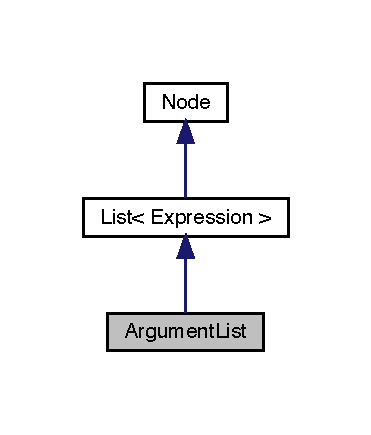
\includegraphics[width=178pt]{struct_argument_list__inherit__graph}
\end{center}
\end{figure}


Collaboration diagram for Argument\+List\+:\nopagebreak
\begin{figure}[H]
\begin{center}
\leavevmode
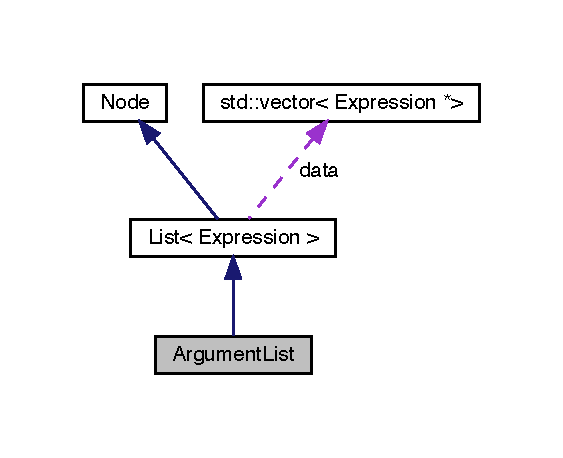
\includegraphics[width=270pt]{struct_argument_list__coll__graph}
\end{center}
\end{figure}
\subsection*{Public Member Functions}
\begin{DoxyCompactItemize}
\item 
{\footnotesize template$<$typename... Args$>$ }\\\hyperlink{struct_argument_list_a7df7f5009c8fc56cede100d66e45cb93}{Argument\+List} (Args \&\&... args)
\item 
void \hyperlink{struct_argument_list_af99815001d6a741b4a9fb0330971a7dc}{accept} (\hyperlink{struct_visitor}{Visitor} \&visitor) const override
\item 
const char $\ast$ \hyperlink{struct_argument_list_a40d37153eb093deadf7045b1ad5ae1fa}{type} () const override
\end{DoxyCompactItemize}
\subsection*{Additional Inherited Members}


\subsection{Constructor \& Destructor Documentation}
\mbox{\Hypertarget{struct_argument_list_a7df7f5009c8fc56cede100d66e45cb93}\label{struct_argument_list_a7df7f5009c8fc56cede100d66e45cb93}} 
\index{Argument\+List@{Argument\+List}!Argument\+List@{Argument\+List}}
\index{Argument\+List@{Argument\+List}!Argument\+List@{Argument\+List}}
\subsubsection{\texorpdfstring{Argument\+List()}{ArgumentList()}}
{\footnotesize\ttfamily template$<$typename... Args$>$ \\
Argument\+List\+::\+Argument\+List (\begin{DoxyParamCaption}\item[{Args \&\&...}]{args }\end{DoxyParamCaption})\hspace{0.3cm}{\ttfamily [inline]}}



\subsection{Member Function Documentation}
\mbox{\Hypertarget{struct_argument_list_af99815001d6a741b4a9fb0330971a7dc}\label{struct_argument_list_af99815001d6a741b4a9fb0330971a7dc}} 
\index{Argument\+List@{Argument\+List}!accept@{accept}}
\index{accept@{accept}!Argument\+List@{Argument\+List}}
\subsubsection{\texorpdfstring{accept()}{accept()}}
{\footnotesize\ttfamily void Argument\+List\+::accept (\begin{DoxyParamCaption}\item[{\hyperlink{struct_visitor}{Visitor} \&}]{visitor }\end{DoxyParamCaption}) const\hspace{0.3cm}{\ttfamily [inline]}, {\ttfamily [override]}, {\ttfamily [virtual]}}



Implements \hyperlink{struct_node_a10bd7af968140bbf5fa461298a969c71}{Node}.

\mbox{\Hypertarget{struct_argument_list_a40d37153eb093deadf7045b1ad5ae1fa}\label{struct_argument_list_a40d37153eb093deadf7045b1ad5ae1fa}} 
\index{Argument\+List@{Argument\+List}!type@{type}}
\index{type@{type}!Argument\+List@{Argument\+List}}
\subsubsection{\texorpdfstring{type()}{type()}}
{\footnotesize\ttfamily const char$\ast$ Argument\+List\+::type (\begin{DoxyParamCaption}{ }\end{DoxyParamCaption}) const\hspace{0.3cm}{\ttfamily [inline]}, {\ttfamily [override]}, {\ttfamily [virtual]}}



Implements \hyperlink{struct_node_a82f29420d0a38efcc370352528e94e9b}{Node}.



The documentation for this struct was generated from the following file\+:\begin{DoxyCompactItemize}
\item 
src/\hyperlink{ast_8h}{ast.\+h}\end{DoxyCompactItemize}

\hypertarget{struct_arguments}{}\section{Arguments Struct Reference}
\label{struct_arguments}\index{Arguments@{Arguments}}


{\ttfamily \#include $<$ast.\+h$>$}



Collaboration diagram for Arguments\+:\nopagebreak
\begin{figure}[H]
\begin{center}
\leavevmode
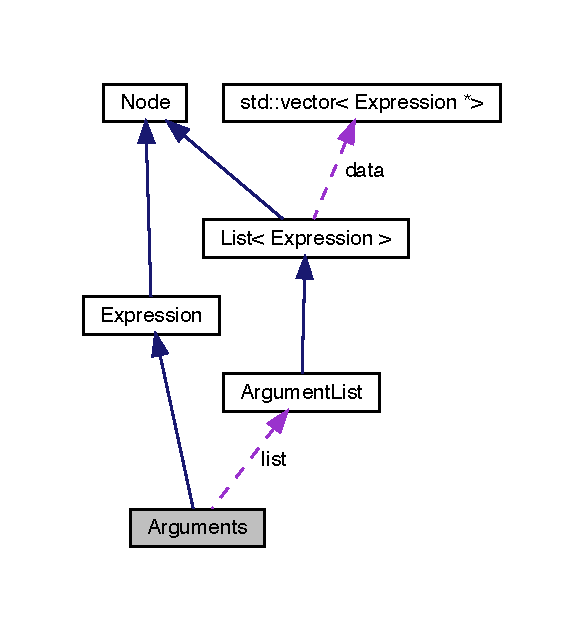
\includegraphics[width=209pt]{struct_arguments__coll__graph}
\end{center}
\end{figure}
\subsection*{Public Attributes}
\begin{DoxyCompactItemize}
\item 
\hyperlink{ast_8h_a31fcc1ca3d32657e8eb6f1433e97d2c9}{Argument\+List} \hyperlink{struct_arguments_aabd86069d52c369cfb9a9041fc991a83}{list}
\end{DoxyCompactItemize}


\subsection{Member Data Documentation}
\mbox{\Hypertarget{struct_arguments_aabd86069d52c369cfb9a9041fc991a83}\label{struct_arguments_aabd86069d52c369cfb9a9041fc991a83}} 
\index{Arguments@{Arguments}!list@{list}}
\index{list@{list}!Arguments@{Arguments}}
\subsubsection{\texorpdfstring{list}{list}}
{\footnotesize\ttfamily \hyperlink{ast_8h_a31fcc1ca3d32657e8eb6f1433e97d2c9}{Argument\+List} Arguments\+::list}



The documentation for this struct was generated from the following file\+:\begin{DoxyCompactItemize}
\item 
src/\hyperlink{ast_8h}{ast.\+h}\end{DoxyCompactItemize}

\hypertarget{struct_array_expression}{}\section{Array\+Expression Struct Reference}
\label{struct_array_expression}\index{Array\+Expression@{Array\+Expression}}


{\ttfamily \#include $<$ast.\+h$>$}



Inheritance diagram for Array\+Expression\+:
\nopagebreak
\begin{figure}[H]
\begin{center}
\leavevmode
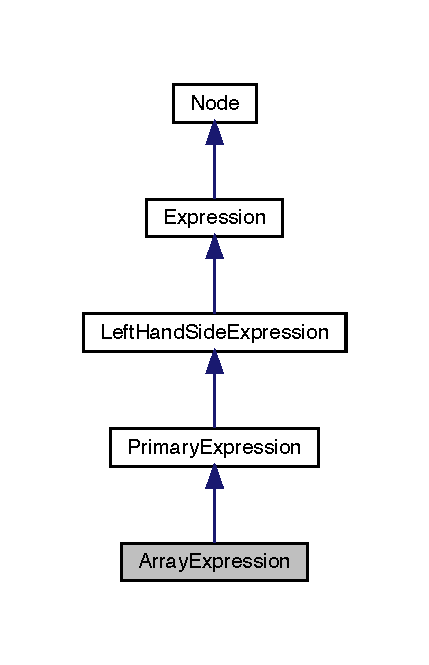
\includegraphics[width=206pt]{struct_array_expression__inherit__graph}
\end{center}
\end{figure}


Collaboration diagram for Array\+Expression\+:
\nopagebreak
\begin{figure}[H]
\begin{center}
\leavevmode
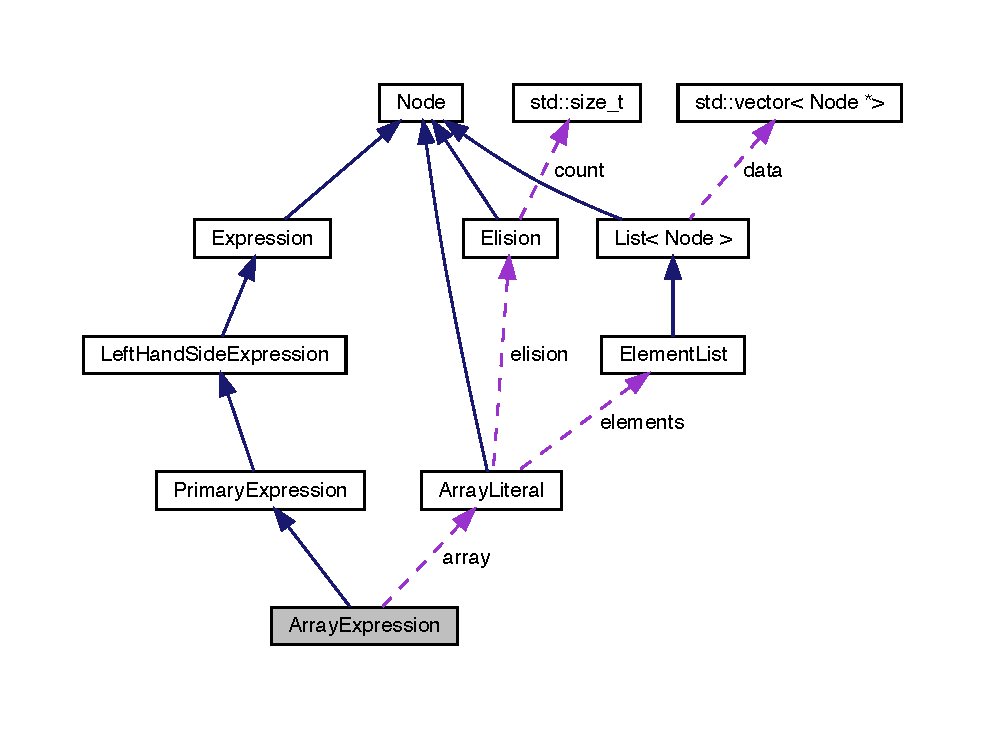
\includegraphics[width=350pt]{struct_array_expression__coll__graph}
\end{center}
\end{figure}
\subsection*{Public Member Functions}
\begin{DoxyCompactItemize}
\item 
\hyperlink{struct_array_expression_ae28e87942dea36d36f3e17460deebbad}{Array\+Expression} (\hyperlink{struct_array_literal}{Array\+Literal} $\ast$\hyperlink{struct_array_expression_a5eaa8dd89911611323de0d6f8221ac1d}{array})
\item 
void \hyperlink{struct_array_expression_a6f1d854ef3cfe2731aee50a45c774b5d}{accept} (\hyperlink{struct_visitor}{Visitor} \&visitor) const override
\item 
const char $\ast$ \hyperlink{struct_array_expression_ad0e148cb5a9de93a554e756cde23103e}{type} () const override
\end{DoxyCompactItemize}
\subsection*{Public Attributes}
\begin{DoxyCompactItemize}
\item 
\hyperlink{struct_array_literal}{Array\+Literal} $\ast$ \hyperlink{struct_array_expression_a5eaa8dd89911611323de0d6f8221ac1d}{array}
\end{DoxyCompactItemize}


\subsection{Constructor \& Destructor Documentation}
\mbox{\Hypertarget{struct_array_expression_ae28e87942dea36d36f3e17460deebbad}\label{struct_array_expression_ae28e87942dea36d36f3e17460deebbad}} 
\index{Array\+Expression@{Array\+Expression}!Array\+Expression@{Array\+Expression}}
\index{Array\+Expression@{Array\+Expression}!Array\+Expression@{Array\+Expression}}
\subsubsection{\texorpdfstring{Array\+Expression()}{ArrayExpression()}}
{\footnotesize\ttfamily Array\+Expression\+::\+Array\+Expression (\begin{DoxyParamCaption}\item[{\hyperlink{struct_array_literal}{Array\+Literal} $\ast$}]{array }\end{DoxyParamCaption})\hspace{0.3cm}{\ttfamily [inline]}}



\subsection{Member Function Documentation}
\mbox{\Hypertarget{struct_array_expression_a6f1d854ef3cfe2731aee50a45c774b5d}\label{struct_array_expression_a6f1d854ef3cfe2731aee50a45c774b5d}} 
\index{Array\+Expression@{Array\+Expression}!accept@{accept}}
\index{accept@{accept}!Array\+Expression@{Array\+Expression}}
\subsubsection{\texorpdfstring{accept()}{accept()}}
{\footnotesize\ttfamily void Array\+Expression\+::accept (\begin{DoxyParamCaption}\item[{\hyperlink{struct_visitor}{Visitor} \&}]{visitor }\end{DoxyParamCaption}) const\hspace{0.3cm}{\ttfamily [inline]}, {\ttfamily [override]}, {\ttfamily [virtual]}}



Implements \hyperlink{struct_node_a10bd7af968140bbf5fa461298a969c71}{Node}.

\mbox{\Hypertarget{struct_array_expression_ad0e148cb5a9de93a554e756cde23103e}\label{struct_array_expression_ad0e148cb5a9de93a554e756cde23103e}} 
\index{Array\+Expression@{Array\+Expression}!type@{type}}
\index{type@{type}!Array\+Expression@{Array\+Expression}}
\subsubsection{\texorpdfstring{type()}{type()}}
{\footnotesize\ttfamily const char$\ast$ Array\+Expression\+::type (\begin{DoxyParamCaption}{ }\end{DoxyParamCaption}) const\hspace{0.3cm}{\ttfamily [inline]}, {\ttfamily [override]}, {\ttfamily [virtual]}}



Implements \hyperlink{struct_node_a82f29420d0a38efcc370352528e94e9b}{Node}.



\subsection{Member Data Documentation}
\mbox{\Hypertarget{struct_array_expression_a5eaa8dd89911611323de0d6f8221ac1d}\label{struct_array_expression_a5eaa8dd89911611323de0d6f8221ac1d}} 
\index{Array\+Expression@{Array\+Expression}!array@{array}}
\index{array@{array}!Array\+Expression@{Array\+Expression}}
\subsubsection{\texorpdfstring{array}{array}}
{\footnotesize\ttfamily \hyperlink{struct_array_literal}{Array\+Literal}$\ast$ Array\+Expression\+::array}



The documentation for this struct was generated from the following file\+:\begin{DoxyCompactItemize}
\item 
src/\hyperlink{ast_8h}{ast.\+h}\end{DoxyCompactItemize}

\hypertarget{struct_array_literal}{}\section{Array\+Literal Struct Reference}
\label{struct_array_literal}\index{Array\+Literal@{Array\+Literal}}


{\ttfamily \#include $<$ast.\+h$>$}



Inheritance diagram for Array\+Literal\+:\nopagebreak
\begin{figure}[H]
\begin{center}
\leavevmode
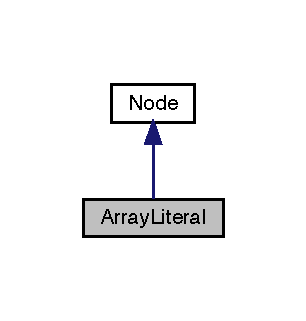
\includegraphics[width=147pt]{struct_array_literal__inherit__graph}
\end{center}
\end{figure}


Collaboration diagram for Array\+Literal\+:\nopagebreak
\begin{figure}[H]
\begin{center}
\leavevmode
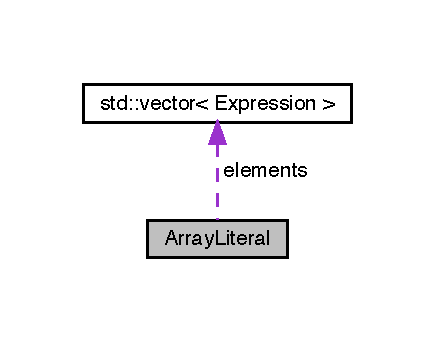
\includegraphics[width=324pt]{struct_array_literal__coll__graph}
\end{center}
\end{figure}
\subsection*{Public Member Functions}
\begin{DoxyCompactItemize}
\item 
\hyperlink{struct_array_literal_a1df7283ca804e7c1147f5024e2e0408d}{Array\+Literal} (\hyperlink{struct_element_list}{Element\+List} $\ast$\hyperlink{struct_array_literal_ae4c3df364c3994cb8916d73a50f1f92f}{elements}=nullptr, \hyperlink{struct_elision}{Elision} $\ast$\hyperlink{struct_array_literal_a08fa9ad6e83376bb2a70d22df9cf2c8a}{elision}=nullptr)
\item 
void \hyperlink{struct_array_literal_ab3ba06d627e0fe714aafb9fc843c83e8}{accept} (\hyperlink{struct_visitor}{Visitor} \&visitor) const override
\item 
const char $\ast$ \hyperlink{struct_array_literal_a24964c1f68d796d071b830b605046f51}{type} () const override
\end{DoxyCompactItemize}
\subsection*{Public Attributes}
\begin{DoxyCompactItemize}
\item 
\hyperlink{struct_element_list}{Element\+List} $\ast$ \hyperlink{struct_array_literal_ae4c3df364c3994cb8916d73a50f1f92f}{elements}
\item 
\hyperlink{struct_elision}{Elision} $\ast$ \hyperlink{struct_array_literal_a08fa9ad6e83376bb2a70d22df9cf2c8a}{elision}
\end{DoxyCompactItemize}


\subsection{Constructor \& Destructor Documentation}
\mbox{\Hypertarget{struct_array_literal_a1df7283ca804e7c1147f5024e2e0408d}\label{struct_array_literal_a1df7283ca804e7c1147f5024e2e0408d}} 
\index{Array\+Literal@{Array\+Literal}!Array\+Literal@{Array\+Literal}}
\index{Array\+Literal@{Array\+Literal}!Array\+Literal@{Array\+Literal}}
\subsubsection{\texorpdfstring{Array\+Literal()}{ArrayLiteral()}}
{\footnotesize\ttfamily Array\+Literal\+::\+Array\+Literal (\begin{DoxyParamCaption}\item[{\hyperlink{struct_element_list}{Element\+List} $\ast$}]{elements = {\ttfamily nullptr},  }\item[{\hyperlink{struct_elision}{Elision} $\ast$}]{elision = {\ttfamily nullptr} }\end{DoxyParamCaption})\hspace{0.3cm}{\ttfamily [inline]}}



\subsection{Member Function Documentation}
\mbox{\Hypertarget{struct_array_literal_ab3ba06d627e0fe714aafb9fc843c83e8}\label{struct_array_literal_ab3ba06d627e0fe714aafb9fc843c83e8}} 
\index{Array\+Literal@{Array\+Literal}!accept@{accept}}
\index{accept@{accept}!Array\+Literal@{Array\+Literal}}
\subsubsection{\texorpdfstring{accept()}{accept()}}
{\footnotesize\ttfamily void Array\+Literal\+::accept (\begin{DoxyParamCaption}\item[{\hyperlink{struct_visitor}{Visitor} \&}]{visitor }\end{DoxyParamCaption}) const\hspace{0.3cm}{\ttfamily [inline]}, {\ttfamily [override]}, {\ttfamily [virtual]}}



Implements \hyperlink{struct_node_a10bd7af968140bbf5fa461298a969c71}{Node}.

\mbox{\Hypertarget{struct_array_literal_a24964c1f68d796d071b830b605046f51}\label{struct_array_literal_a24964c1f68d796d071b830b605046f51}} 
\index{Array\+Literal@{Array\+Literal}!type@{type}}
\index{type@{type}!Array\+Literal@{Array\+Literal}}
\subsubsection{\texorpdfstring{type()}{type()}}
{\footnotesize\ttfamily const char$\ast$ Array\+Literal\+::type (\begin{DoxyParamCaption}{ }\end{DoxyParamCaption}) const\hspace{0.3cm}{\ttfamily [inline]}, {\ttfamily [override]}, {\ttfamily [virtual]}}



Implements \hyperlink{struct_node_a82f29420d0a38efcc370352528e94e9b}{Node}.



\subsection{Member Data Documentation}
\mbox{\Hypertarget{struct_array_literal_ae4c3df364c3994cb8916d73a50f1f92f}\label{struct_array_literal_ae4c3df364c3994cb8916d73a50f1f92f}} 
\index{Array\+Literal@{Array\+Literal}!elements@{elements}}
\index{elements@{elements}!Array\+Literal@{Array\+Literal}}
\subsubsection{\texorpdfstring{elements}{elements}}
{\footnotesize\ttfamily \hyperlink{struct_element_list}{Element\+List}$\ast$ Array\+Literal\+::elements}

\mbox{\Hypertarget{struct_array_literal_a08fa9ad6e83376bb2a70d22df9cf2c8a}\label{struct_array_literal_a08fa9ad6e83376bb2a70d22df9cf2c8a}} 
\index{Array\+Literal@{Array\+Literal}!elision@{elision}}
\index{elision@{elision}!Array\+Literal@{Array\+Literal}}
\subsubsection{\texorpdfstring{elision}{elision}}
{\footnotesize\ttfamily \hyperlink{struct_elision}{Elision}$\ast$ Array\+Literal\+::elision}



The documentation for this struct was generated from the following file\+:\begin{DoxyCompactItemize}
\item 
src/\hyperlink{ast_8h}{ast.\+h}\end{DoxyCompactItemize}

\hypertarget{struct_catch_1_1_assertion_info}{}\section{Catch\+:\+:Assertion\+Info Struct Reference}
\label{struct_catch_1_1_assertion_info}\index{Catch\+::\+Assertion\+Info@{Catch\+::\+Assertion\+Info}}


{\ttfamily \#include $<$catch.\+hpp$>$}



Collaboration diagram for Catch\+:\+:Assertion\+Info\+:
\nopagebreak
\begin{figure}[H]
\begin{center}
\leavevmode
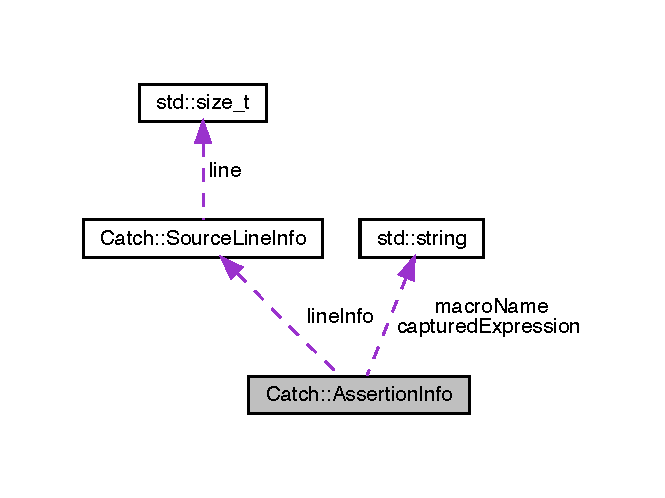
\includegraphics[width=319pt]{struct_catch_1_1_assertion_info__coll__graph}
\end{center}
\end{figure}
\subsection*{Public Member Functions}
\begin{DoxyCompactItemize}
\item 
\hyperlink{struct_catch_1_1_assertion_info_a15c29d306c86361f842a0351a6003b9f}{Assertion\+Info} ()
\item 
\hyperlink{struct_catch_1_1_assertion_info_aaf6cc3eebd40391e54d37ed42953c73f}{Assertion\+Info} (\textbf{ std\+::string} const \&\+\_\+macro\+Name, \hyperlink{struct_catch_1_1_source_line_info}{Source\+Line\+Info} const \&\+\_\+line\+Info, \textbf{ std\+::string} const \&\+\_\+captured\+Expression, \hyperlink{struct_catch_1_1_result_disposition_a3396cad6e2259af326b3aae93e23e9d8}{Result\+Disposition\+::\+Flags} \+\_\+result\+Disposition)
\end{DoxyCompactItemize}
\subsection*{Public Attributes}
\begin{DoxyCompactItemize}
\item 
\textbf{ std\+::string} \hyperlink{struct_catch_1_1_assertion_info_ac2e59e8c89e00eb3390768f50d540b18}{macro\+Name}
\item 
\hyperlink{struct_catch_1_1_source_line_info}{Source\+Line\+Info} \hyperlink{struct_catch_1_1_assertion_info_a17bdbb404ba12658034f833be2f4c3e7}{line\+Info}
\item 
\textbf{ std\+::string} \hyperlink{struct_catch_1_1_assertion_info_af7c1d3cbfa346e9a303030fa0ef0cb54}{captured\+Expression}
\item 
\hyperlink{struct_catch_1_1_result_disposition_a3396cad6e2259af326b3aae93e23e9d8}{Result\+Disposition\+::\+Flags} \hyperlink{struct_catch_1_1_assertion_info_a60353b3632ab2f827162f2b2d6911073}{result\+Disposition}
\end{DoxyCompactItemize}


\subsection{Constructor \& Destructor Documentation}
\mbox{\Hypertarget{struct_catch_1_1_assertion_info_a15c29d306c86361f842a0351a6003b9f}\label{struct_catch_1_1_assertion_info_a15c29d306c86361f842a0351a6003b9f}} 
\index{Catch\+::\+Assertion\+Info@{Catch\+::\+Assertion\+Info}!Assertion\+Info@{Assertion\+Info}}
\index{Assertion\+Info@{Assertion\+Info}!Catch\+::\+Assertion\+Info@{Catch\+::\+Assertion\+Info}}
\subsubsection{\texorpdfstring{Assertion\+Info()}{AssertionInfo()}\hspace{0.1cm}{\footnotesize\ttfamily [1/2]}}
{\footnotesize\ttfamily Catch\+::\+Assertion\+Info\+::\+Assertion\+Info (\begin{DoxyParamCaption}{ }\end{DoxyParamCaption})\hspace{0.3cm}{\ttfamily [inline]}}

\mbox{\Hypertarget{struct_catch_1_1_assertion_info_aaf6cc3eebd40391e54d37ed42953c73f}\label{struct_catch_1_1_assertion_info_aaf6cc3eebd40391e54d37ed42953c73f}} 
\index{Catch\+::\+Assertion\+Info@{Catch\+::\+Assertion\+Info}!Assertion\+Info@{Assertion\+Info}}
\index{Assertion\+Info@{Assertion\+Info}!Catch\+::\+Assertion\+Info@{Catch\+::\+Assertion\+Info}}
\subsubsection{\texorpdfstring{Assertion\+Info()}{AssertionInfo()}\hspace{0.1cm}{\footnotesize\ttfamily [2/2]}}
{\footnotesize\ttfamily Catch\+::\+Assertion\+Info\+::\+Assertion\+Info (\begin{DoxyParamCaption}\item[{\textbf{ std\+::string} const \&}]{\+\_\+macro\+Name,  }\item[{\hyperlink{struct_catch_1_1_source_line_info}{Source\+Line\+Info} const \&}]{\+\_\+line\+Info,  }\item[{\textbf{ std\+::string} const \&}]{\+\_\+captured\+Expression,  }\item[{\hyperlink{struct_catch_1_1_result_disposition_a3396cad6e2259af326b3aae93e23e9d8}{Result\+Disposition\+::\+Flags}}]{\+\_\+result\+Disposition }\end{DoxyParamCaption})}



\subsection{Member Data Documentation}
\mbox{\Hypertarget{struct_catch_1_1_assertion_info_af7c1d3cbfa346e9a303030fa0ef0cb54}\label{struct_catch_1_1_assertion_info_af7c1d3cbfa346e9a303030fa0ef0cb54}} 
\index{Catch\+::\+Assertion\+Info@{Catch\+::\+Assertion\+Info}!captured\+Expression@{captured\+Expression}}
\index{captured\+Expression@{captured\+Expression}!Catch\+::\+Assertion\+Info@{Catch\+::\+Assertion\+Info}}
\subsubsection{\texorpdfstring{captured\+Expression}{capturedExpression}}
{\footnotesize\ttfamily \textbf{ std\+::string} Catch\+::\+Assertion\+Info\+::captured\+Expression}

\mbox{\Hypertarget{struct_catch_1_1_assertion_info_a17bdbb404ba12658034f833be2f4c3e7}\label{struct_catch_1_1_assertion_info_a17bdbb404ba12658034f833be2f4c3e7}} 
\index{Catch\+::\+Assertion\+Info@{Catch\+::\+Assertion\+Info}!line\+Info@{line\+Info}}
\index{line\+Info@{line\+Info}!Catch\+::\+Assertion\+Info@{Catch\+::\+Assertion\+Info}}
\subsubsection{\texorpdfstring{line\+Info}{lineInfo}}
{\footnotesize\ttfamily \hyperlink{struct_catch_1_1_source_line_info}{Source\+Line\+Info} Catch\+::\+Assertion\+Info\+::line\+Info}

\mbox{\Hypertarget{struct_catch_1_1_assertion_info_ac2e59e8c89e00eb3390768f50d540b18}\label{struct_catch_1_1_assertion_info_ac2e59e8c89e00eb3390768f50d540b18}} 
\index{Catch\+::\+Assertion\+Info@{Catch\+::\+Assertion\+Info}!macro\+Name@{macro\+Name}}
\index{macro\+Name@{macro\+Name}!Catch\+::\+Assertion\+Info@{Catch\+::\+Assertion\+Info}}
\subsubsection{\texorpdfstring{macro\+Name}{macroName}}
{\footnotesize\ttfamily \textbf{ std\+::string} Catch\+::\+Assertion\+Info\+::macro\+Name}

\mbox{\Hypertarget{struct_catch_1_1_assertion_info_a60353b3632ab2f827162f2b2d6911073}\label{struct_catch_1_1_assertion_info_a60353b3632ab2f827162f2b2d6911073}} 
\index{Catch\+::\+Assertion\+Info@{Catch\+::\+Assertion\+Info}!result\+Disposition@{result\+Disposition}}
\index{result\+Disposition@{result\+Disposition}!Catch\+::\+Assertion\+Info@{Catch\+::\+Assertion\+Info}}
\subsubsection{\texorpdfstring{result\+Disposition}{resultDisposition}}
{\footnotesize\ttfamily \hyperlink{struct_catch_1_1_result_disposition_a3396cad6e2259af326b3aae93e23e9d8}{Result\+Disposition\+::\+Flags} Catch\+::\+Assertion\+Info\+::result\+Disposition}



The documentation for this struct was generated from the following file\+:\begin{DoxyCompactItemize}
\item 
src/\hyperlink{catch_8hpp}{catch.\+hpp}\end{DoxyCompactItemize}

\hypertarget{class_catch_1_1_assertion_result}{}\section{Catch\+:\+:Assertion\+Result Class Reference}
\label{class_catch_1_1_assertion_result}\index{Catch\+::\+Assertion\+Result@{Catch\+::\+Assertion\+Result}}


{\ttfamily \#include $<$catch.\+hpp$>$}



Collaboration diagram for Catch\+:\+:Assertion\+Result\+:
\nopagebreak
\begin{figure}[H]
\begin{center}
\leavevmode
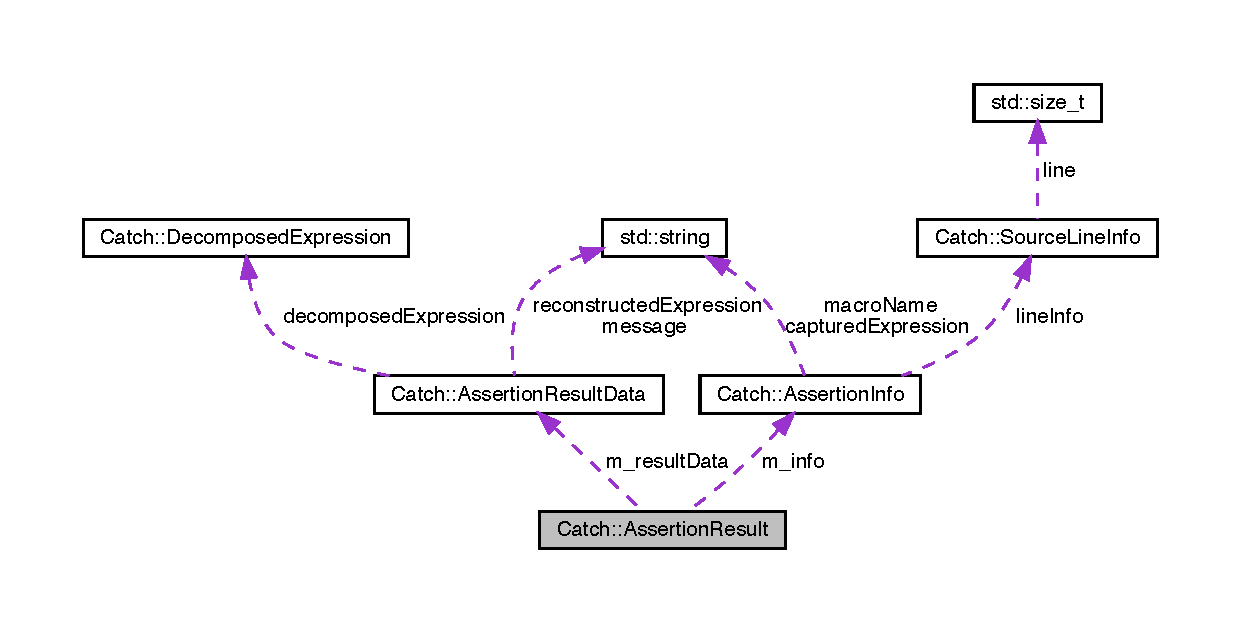
\includegraphics[width=350pt]{class_catch_1_1_assertion_result__coll__graph}
\end{center}
\end{figure}
\subsection*{Public Member Functions}
\begin{DoxyCompactItemize}
\item 
\hyperlink{class_catch_1_1_assertion_result_a570b999c5f66e33cb31d3adb29fec25b}{Assertion\+Result} ()
\item 
\hyperlink{class_catch_1_1_assertion_result_ab58aeec27052ba400633ed0e36cea692}{Assertion\+Result} (\hyperlink{struct_catch_1_1_assertion_info}{Assertion\+Info} const \&info, \hyperlink{struct_catch_1_1_assertion_result_data}{Assertion\+Result\+Data} const \&data)
\item 
\hyperlink{class_catch_1_1_assertion_result_abf90f5abd04d38b2fb4f5d575bdc4f1e}{$\sim$\+Assertion\+Result} ()
\item 
bool \hyperlink{class_catch_1_1_assertion_result_ae39658b71c4afc3c8a859043b0e97027}{is\+Ok} () const
\item 
bool \hyperlink{class_catch_1_1_assertion_result_ac5cc872b721d5fb65d87221d30b22fdd}{succeeded} () const
\item 
\hyperlink{struct_catch_1_1_result_was_a624e1ee3661fcf6094ceef1f654601ef}{Result\+Was\+::\+Of\+Type} \hyperlink{class_catch_1_1_assertion_result_ac810750194e1722489d2fd16e8c6a4a8}{get\+Result\+Type} () const
\item 
bool \hyperlink{class_catch_1_1_assertion_result_aba37b4fef1015989df2136592958e984}{has\+Expression} () const
\item 
bool \hyperlink{class_catch_1_1_assertion_result_aae37064b401919fa8ac480ef86cca924}{has\+Message} () const
\item 
\textbf{ std\+::string} \hyperlink{class_catch_1_1_assertion_result_a26a777f3959353c729544cb2ace0d279}{get\+Expression} () const
\item 
\textbf{ std\+::string} \hyperlink{class_catch_1_1_assertion_result_aac35a0ca42d33bff6467c76573730f5e}{get\+Expression\+In\+Macro} () const
\item 
bool \hyperlink{class_catch_1_1_assertion_result_a78c43506c2b3d8cc1fb141a97d09ec94}{has\+Expanded\+Expression} () const
\item 
\textbf{ std\+::string} \hyperlink{class_catch_1_1_assertion_result_aaa46070791a6c07caaed86229b8d9d75}{get\+Expanded\+Expression} () const
\item 
\textbf{ std\+::string} \hyperlink{class_catch_1_1_assertion_result_ae730943beed46921b09383c673e35786}{get\+Message} () const
\item 
\hyperlink{struct_catch_1_1_source_line_info}{Source\+Line\+Info} \hyperlink{class_catch_1_1_assertion_result_aa4d3fdbfe276a69a035762dbb790800f}{get\+Source\+Info} () const
\item 
\textbf{ std\+::string} \hyperlink{class_catch_1_1_assertion_result_aaefd9a0384282fd08a4a72aa19bd0628}{get\+Test\+Macro\+Name} () const
\item 
void \hyperlink{class_catch_1_1_assertion_result_a406884d8b8209c80078706724c528df5}{discard\+Decomposed\+Expression} () const
\item 
void \hyperlink{class_catch_1_1_assertion_result_ac0b1d268a3ffa1f1fb305cad9435d824}{expand\+Decomposed\+Expression} () const
\end{DoxyCompactItemize}
\subsection*{Protected Attributes}
\begin{DoxyCompactItemize}
\item 
\hyperlink{struct_catch_1_1_assertion_info}{Assertion\+Info} \hyperlink{class_catch_1_1_assertion_result_a3e7236f73a51d6fc8bb9dfdefcee7772}{m\+\_\+info}
\item 
\hyperlink{struct_catch_1_1_assertion_result_data}{Assertion\+Result\+Data} \hyperlink{class_catch_1_1_assertion_result_add3455b8bbedb0d643e18da67c66b4f7}{m\+\_\+result\+Data}
\end{DoxyCompactItemize}


\subsection{Constructor \& Destructor Documentation}
\mbox{\Hypertarget{class_catch_1_1_assertion_result_a570b999c5f66e33cb31d3adb29fec25b}\label{class_catch_1_1_assertion_result_a570b999c5f66e33cb31d3adb29fec25b}} 
\index{Catch\+::\+Assertion\+Result@{Catch\+::\+Assertion\+Result}!Assertion\+Result@{Assertion\+Result}}
\index{Assertion\+Result@{Assertion\+Result}!Catch\+::\+Assertion\+Result@{Catch\+::\+Assertion\+Result}}
\subsubsection{\texorpdfstring{Assertion\+Result()}{AssertionResult()}\hspace{0.1cm}{\footnotesize\ttfamily [1/2]}}
{\footnotesize\ttfamily Catch\+::\+Assertion\+Result\+::\+Assertion\+Result (\begin{DoxyParamCaption}{ }\end{DoxyParamCaption})}

\mbox{\Hypertarget{class_catch_1_1_assertion_result_ab58aeec27052ba400633ed0e36cea692}\label{class_catch_1_1_assertion_result_ab58aeec27052ba400633ed0e36cea692}} 
\index{Catch\+::\+Assertion\+Result@{Catch\+::\+Assertion\+Result}!Assertion\+Result@{Assertion\+Result}}
\index{Assertion\+Result@{Assertion\+Result}!Catch\+::\+Assertion\+Result@{Catch\+::\+Assertion\+Result}}
\subsubsection{\texorpdfstring{Assertion\+Result()}{AssertionResult()}\hspace{0.1cm}{\footnotesize\ttfamily [2/2]}}
{\footnotesize\ttfamily Catch\+::\+Assertion\+Result\+::\+Assertion\+Result (\begin{DoxyParamCaption}\item[{\hyperlink{struct_catch_1_1_assertion_info}{Assertion\+Info} const \&}]{info,  }\item[{\hyperlink{struct_catch_1_1_assertion_result_data}{Assertion\+Result\+Data} const \&}]{data }\end{DoxyParamCaption})}

\mbox{\Hypertarget{class_catch_1_1_assertion_result_abf90f5abd04d38b2fb4f5d575bdc4f1e}\label{class_catch_1_1_assertion_result_abf90f5abd04d38b2fb4f5d575bdc4f1e}} 
\index{Catch\+::\+Assertion\+Result@{Catch\+::\+Assertion\+Result}!````~Assertion\+Result@{$\sim$\+Assertion\+Result}}
\index{````~Assertion\+Result@{$\sim$\+Assertion\+Result}!Catch\+::\+Assertion\+Result@{Catch\+::\+Assertion\+Result}}
\subsubsection{\texorpdfstring{$\sim$\+Assertion\+Result()}{~AssertionResult()}}
{\footnotesize\ttfamily Catch\+::\+Assertion\+Result\+::$\sim$\+Assertion\+Result (\begin{DoxyParamCaption}{ }\end{DoxyParamCaption})}



\subsection{Member Function Documentation}
\mbox{\Hypertarget{class_catch_1_1_assertion_result_a406884d8b8209c80078706724c528df5}\label{class_catch_1_1_assertion_result_a406884d8b8209c80078706724c528df5}} 
\index{Catch\+::\+Assertion\+Result@{Catch\+::\+Assertion\+Result}!discard\+Decomposed\+Expression@{discard\+Decomposed\+Expression}}
\index{discard\+Decomposed\+Expression@{discard\+Decomposed\+Expression}!Catch\+::\+Assertion\+Result@{Catch\+::\+Assertion\+Result}}
\subsubsection{\texorpdfstring{discard\+Decomposed\+Expression()}{discardDecomposedExpression()}}
{\footnotesize\ttfamily void Catch\+::\+Assertion\+Result\+::discard\+Decomposed\+Expression (\begin{DoxyParamCaption}{ }\end{DoxyParamCaption}) const}

\mbox{\Hypertarget{class_catch_1_1_assertion_result_ac0b1d268a3ffa1f1fb305cad9435d824}\label{class_catch_1_1_assertion_result_ac0b1d268a3ffa1f1fb305cad9435d824}} 
\index{Catch\+::\+Assertion\+Result@{Catch\+::\+Assertion\+Result}!expand\+Decomposed\+Expression@{expand\+Decomposed\+Expression}}
\index{expand\+Decomposed\+Expression@{expand\+Decomposed\+Expression}!Catch\+::\+Assertion\+Result@{Catch\+::\+Assertion\+Result}}
\subsubsection{\texorpdfstring{expand\+Decomposed\+Expression()}{expandDecomposedExpression()}}
{\footnotesize\ttfamily void Catch\+::\+Assertion\+Result\+::expand\+Decomposed\+Expression (\begin{DoxyParamCaption}{ }\end{DoxyParamCaption}) const}

\mbox{\Hypertarget{class_catch_1_1_assertion_result_aaa46070791a6c07caaed86229b8d9d75}\label{class_catch_1_1_assertion_result_aaa46070791a6c07caaed86229b8d9d75}} 
\index{Catch\+::\+Assertion\+Result@{Catch\+::\+Assertion\+Result}!get\+Expanded\+Expression@{get\+Expanded\+Expression}}
\index{get\+Expanded\+Expression@{get\+Expanded\+Expression}!Catch\+::\+Assertion\+Result@{Catch\+::\+Assertion\+Result}}
\subsubsection{\texorpdfstring{get\+Expanded\+Expression()}{getExpandedExpression()}}
{\footnotesize\ttfamily \textbf{ std\+::string} Catch\+::\+Assertion\+Result\+::get\+Expanded\+Expression (\begin{DoxyParamCaption}{ }\end{DoxyParamCaption}) const}

\mbox{\Hypertarget{class_catch_1_1_assertion_result_a26a777f3959353c729544cb2ace0d279}\label{class_catch_1_1_assertion_result_a26a777f3959353c729544cb2ace0d279}} 
\index{Catch\+::\+Assertion\+Result@{Catch\+::\+Assertion\+Result}!get\+Expression@{get\+Expression}}
\index{get\+Expression@{get\+Expression}!Catch\+::\+Assertion\+Result@{Catch\+::\+Assertion\+Result}}
\subsubsection{\texorpdfstring{get\+Expression()}{getExpression()}}
{\footnotesize\ttfamily \textbf{ std\+::string} Catch\+::\+Assertion\+Result\+::get\+Expression (\begin{DoxyParamCaption}{ }\end{DoxyParamCaption}) const}

\mbox{\Hypertarget{class_catch_1_1_assertion_result_aac35a0ca42d33bff6467c76573730f5e}\label{class_catch_1_1_assertion_result_aac35a0ca42d33bff6467c76573730f5e}} 
\index{Catch\+::\+Assertion\+Result@{Catch\+::\+Assertion\+Result}!get\+Expression\+In\+Macro@{get\+Expression\+In\+Macro}}
\index{get\+Expression\+In\+Macro@{get\+Expression\+In\+Macro}!Catch\+::\+Assertion\+Result@{Catch\+::\+Assertion\+Result}}
\subsubsection{\texorpdfstring{get\+Expression\+In\+Macro()}{getExpressionInMacro()}}
{\footnotesize\ttfamily \textbf{ std\+::string} Catch\+::\+Assertion\+Result\+::get\+Expression\+In\+Macro (\begin{DoxyParamCaption}{ }\end{DoxyParamCaption}) const}

\mbox{\Hypertarget{class_catch_1_1_assertion_result_ae730943beed46921b09383c673e35786}\label{class_catch_1_1_assertion_result_ae730943beed46921b09383c673e35786}} 
\index{Catch\+::\+Assertion\+Result@{Catch\+::\+Assertion\+Result}!get\+Message@{get\+Message}}
\index{get\+Message@{get\+Message}!Catch\+::\+Assertion\+Result@{Catch\+::\+Assertion\+Result}}
\subsubsection{\texorpdfstring{get\+Message()}{getMessage()}}
{\footnotesize\ttfamily \textbf{ std\+::string} Catch\+::\+Assertion\+Result\+::get\+Message (\begin{DoxyParamCaption}{ }\end{DoxyParamCaption}) const}

\mbox{\Hypertarget{class_catch_1_1_assertion_result_ac810750194e1722489d2fd16e8c6a4a8}\label{class_catch_1_1_assertion_result_ac810750194e1722489d2fd16e8c6a4a8}} 
\index{Catch\+::\+Assertion\+Result@{Catch\+::\+Assertion\+Result}!get\+Result\+Type@{get\+Result\+Type}}
\index{get\+Result\+Type@{get\+Result\+Type}!Catch\+::\+Assertion\+Result@{Catch\+::\+Assertion\+Result}}
\subsubsection{\texorpdfstring{get\+Result\+Type()}{getResultType()}}
{\footnotesize\ttfamily \hyperlink{struct_catch_1_1_result_was_a624e1ee3661fcf6094ceef1f654601ef}{Result\+Was\+::\+Of\+Type} Catch\+::\+Assertion\+Result\+::get\+Result\+Type (\begin{DoxyParamCaption}{ }\end{DoxyParamCaption}) const}

\mbox{\Hypertarget{class_catch_1_1_assertion_result_aa4d3fdbfe276a69a035762dbb790800f}\label{class_catch_1_1_assertion_result_aa4d3fdbfe276a69a035762dbb790800f}} 
\index{Catch\+::\+Assertion\+Result@{Catch\+::\+Assertion\+Result}!get\+Source\+Info@{get\+Source\+Info}}
\index{get\+Source\+Info@{get\+Source\+Info}!Catch\+::\+Assertion\+Result@{Catch\+::\+Assertion\+Result}}
\subsubsection{\texorpdfstring{get\+Source\+Info()}{getSourceInfo()}}
{\footnotesize\ttfamily \hyperlink{struct_catch_1_1_source_line_info}{Source\+Line\+Info} Catch\+::\+Assertion\+Result\+::get\+Source\+Info (\begin{DoxyParamCaption}{ }\end{DoxyParamCaption}) const}

\mbox{\Hypertarget{class_catch_1_1_assertion_result_aaefd9a0384282fd08a4a72aa19bd0628}\label{class_catch_1_1_assertion_result_aaefd9a0384282fd08a4a72aa19bd0628}} 
\index{Catch\+::\+Assertion\+Result@{Catch\+::\+Assertion\+Result}!get\+Test\+Macro\+Name@{get\+Test\+Macro\+Name}}
\index{get\+Test\+Macro\+Name@{get\+Test\+Macro\+Name}!Catch\+::\+Assertion\+Result@{Catch\+::\+Assertion\+Result}}
\subsubsection{\texorpdfstring{get\+Test\+Macro\+Name()}{getTestMacroName()}}
{\footnotesize\ttfamily \textbf{ std\+::string} Catch\+::\+Assertion\+Result\+::get\+Test\+Macro\+Name (\begin{DoxyParamCaption}{ }\end{DoxyParamCaption}) const}

\mbox{\Hypertarget{class_catch_1_1_assertion_result_a78c43506c2b3d8cc1fb141a97d09ec94}\label{class_catch_1_1_assertion_result_a78c43506c2b3d8cc1fb141a97d09ec94}} 
\index{Catch\+::\+Assertion\+Result@{Catch\+::\+Assertion\+Result}!has\+Expanded\+Expression@{has\+Expanded\+Expression}}
\index{has\+Expanded\+Expression@{has\+Expanded\+Expression}!Catch\+::\+Assertion\+Result@{Catch\+::\+Assertion\+Result}}
\subsubsection{\texorpdfstring{has\+Expanded\+Expression()}{hasExpandedExpression()}}
{\footnotesize\ttfamily bool Catch\+::\+Assertion\+Result\+::has\+Expanded\+Expression (\begin{DoxyParamCaption}{ }\end{DoxyParamCaption}) const}

\mbox{\Hypertarget{class_catch_1_1_assertion_result_aba37b4fef1015989df2136592958e984}\label{class_catch_1_1_assertion_result_aba37b4fef1015989df2136592958e984}} 
\index{Catch\+::\+Assertion\+Result@{Catch\+::\+Assertion\+Result}!has\+Expression@{has\+Expression}}
\index{has\+Expression@{has\+Expression}!Catch\+::\+Assertion\+Result@{Catch\+::\+Assertion\+Result}}
\subsubsection{\texorpdfstring{has\+Expression()}{hasExpression()}}
{\footnotesize\ttfamily bool Catch\+::\+Assertion\+Result\+::has\+Expression (\begin{DoxyParamCaption}{ }\end{DoxyParamCaption}) const}

\mbox{\Hypertarget{class_catch_1_1_assertion_result_aae37064b401919fa8ac480ef86cca924}\label{class_catch_1_1_assertion_result_aae37064b401919fa8ac480ef86cca924}} 
\index{Catch\+::\+Assertion\+Result@{Catch\+::\+Assertion\+Result}!has\+Message@{has\+Message}}
\index{has\+Message@{has\+Message}!Catch\+::\+Assertion\+Result@{Catch\+::\+Assertion\+Result}}
\subsubsection{\texorpdfstring{has\+Message()}{hasMessage()}}
{\footnotesize\ttfamily bool Catch\+::\+Assertion\+Result\+::has\+Message (\begin{DoxyParamCaption}{ }\end{DoxyParamCaption}) const}

\mbox{\Hypertarget{class_catch_1_1_assertion_result_ae39658b71c4afc3c8a859043b0e97027}\label{class_catch_1_1_assertion_result_ae39658b71c4afc3c8a859043b0e97027}} 
\index{Catch\+::\+Assertion\+Result@{Catch\+::\+Assertion\+Result}!is\+Ok@{is\+Ok}}
\index{is\+Ok@{is\+Ok}!Catch\+::\+Assertion\+Result@{Catch\+::\+Assertion\+Result}}
\subsubsection{\texorpdfstring{is\+Ok()}{isOk()}}
{\footnotesize\ttfamily bool Catch\+::\+Assertion\+Result\+::is\+Ok (\begin{DoxyParamCaption}{ }\end{DoxyParamCaption}) const}

\mbox{\Hypertarget{class_catch_1_1_assertion_result_ac5cc872b721d5fb65d87221d30b22fdd}\label{class_catch_1_1_assertion_result_ac5cc872b721d5fb65d87221d30b22fdd}} 
\index{Catch\+::\+Assertion\+Result@{Catch\+::\+Assertion\+Result}!succeeded@{succeeded}}
\index{succeeded@{succeeded}!Catch\+::\+Assertion\+Result@{Catch\+::\+Assertion\+Result}}
\subsubsection{\texorpdfstring{succeeded()}{succeeded()}}
{\footnotesize\ttfamily bool Catch\+::\+Assertion\+Result\+::succeeded (\begin{DoxyParamCaption}{ }\end{DoxyParamCaption}) const}



\subsection{Member Data Documentation}
\mbox{\Hypertarget{class_catch_1_1_assertion_result_a3e7236f73a51d6fc8bb9dfdefcee7772}\label{class_catch_1_1_assertion_result_a3e7236f73a51d6fc8bb9dfdefcee7772}} 
\index{Catch\+::\+Assertion\+Result@{Catch\+::\+Assertion\+Result}!m\+\_\+info@{m\+\_\+info}}
\index{m\+\_\+info@{m\+\_\+info}!Catch\+::\+Assertion\+Result@{Catch\+::\+Assertion\+Result}}
\subsubsection{\texorpdfstring{m\+\_\+info}{m\_info}}
{\footnotesize\ttfamily \hyperlink{struct_catch_1_1_assertion_info}{Assertion\+Info} Catch\+::\+Assertion\+Result\+::m\+\_\+info\hspace{0.3cm}{\ttfamily [protected]}}

\mbox{\Hypertarget{class_catch_1_1_assertion_result_add3455b8bbedb0d643e18da67c66b4f7}\label{class_catch_1_1_assertion_result_add3455b8bbedb0d643e18da67c66b4f7}} 
\index{Catch\+::\+Assertion\+Result@{Catch\+::\+Assertion\+Result}!m\+\_\+result\+Data@{m\+\_\+result\+Data}}
\index{m\+\_\+result\+Data@{m\+\_\+result\+Data}!Catch\+::\+Assertion\+Result@{Catch\+::\+Assertion\+Result}}
\subsubsection{\texorpdfstring{m\+\_\+result\+Data}{m\_resultData}}
{\footnotesize\ttfamily \hyperlink{struct_catch_1_1_assertion_result_data}{Assertion\+Result\+Data} Catch\+::\+Assertion\+Result\+::m\+\_\+result\+Data\hspace{0.3cm}{\ttfamily [protected]}}



The documentation for this class was generated from the following file\+:\begin{DoxyCompactItemize}
\item 
src/\hyperlink{catch_8hpp}{catch.\+hpp}\end{DoxyCompactItemize}

\hypertarget{struct_catch_1_1_assertion_result_data}{}\section{Catch\+:\+:Assertion\+Result\+Data Struct Reference}
\label{struct_catch_1_1_assertion_result_data}\index{Catch\+::\+Assertion\+Result\+Data@{Catch\+::\+Assertion\+Result\+Data}}


{\ttfamily \#include $<$catch.\+hpp$>$}



Collaboration diagram for Catch\+:\+:Assertion\+Result\+Data\+:
\nopagebreak
\begin{figure}[H]
\begin{center}
\leavevmode
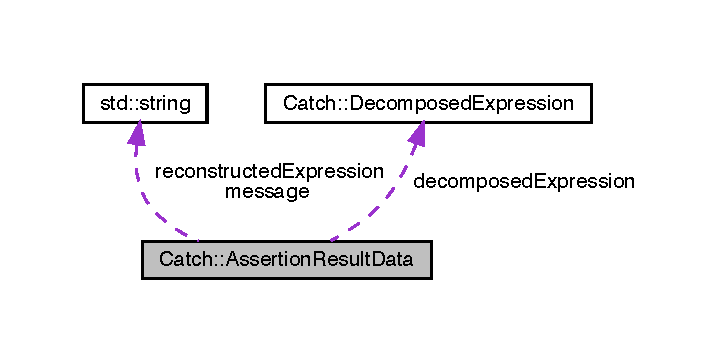
\includegraphics[width=345pt]{struct_catch_1_1_assertion_result_data__coll__graph}
\end{center}
\end{figure}
\subsection*{Public Member Functions}
\begin{DoxyCompactItemize}
\item 
\hyperlink{struct_catch_1_1_assertion_result_data_a37179edde9f853f22d4456677fd97701}{Assertion\+Result\+Data} ()
\item 
void \hyperlink{struct_catch_1_1_assertion_result_data_a3b4df7cd1f8228ea1144b5cd0af6006a}{negate} (bool parenthesize)
\item 
\textbf{ std\+::string} const  \& \hyperlink{struct_catch_1_1_assertion_result_data_adbc0629083cd2e76c3a78696453443b0}{reconstruct\+Expression} () const
\end{DoxyCompactItemize}
\subsection*{Public Attributes}
\begin{DoxyCompactItemize}
\item 
\hyperlink{struct_catch_1_1_decomposed_expression}{Decomposed\+Expression} const  $\ast$ \hyperlink{struct_catch_1_1_assertion_result_data_a45b2bf2ed11da83d09dd78a2b7a44cd4}{decomposed\+Expression}
\item 
\textbf{ std\+::string} \hyperlink{struct_catch_1_1_assertion_result_data_a9e809d36fffbeb1c7d0cbe7382dd9595}{reconstructed\+Expression}
\item 
\textbf{ std\+::string} \hyperlink{struct_catch_1_1_assertion_result_data_ac34215803c4c4a88f795879f61c1f7b4}{message}
\item 
\hyperlink{struct_catch_1_1_result_was_a624e1ee3661fcf6094ceef1f654601ef}{Result\+Was\+::\+Of\+Type} \hyperlink{struct_catch_1_1_assertion_result_data_a7ceab4a7ff722aec5587e3748caf66b7}{result\+Type}
\item 
bool \hyperlink{struct_catch_1_1_assertion_result_data_a17773c6f999cfded12e470b0321694a1}{negated}
\item 
bool \hyperlink{struct_catch_1_1_assertion_result_data_a8418e3744b5486cb7f0d79c84569078e}{parenthesized}
\end{DoxyCompactItemize}


\subsection{Constructor \& Destructor Documentation}
\mbox{\Hypertarget{struct_catch_1_1_assertion_result_data_a37179edde9f853f22d4456677fd97701}\label{struct_catch_1_1_assertion_result_data_a37179edde9f853f22d4456677fd97701}} 
\index{Catch\+::\+Assertion\+Result\+Data@{Catch\+::\+Assertion\+Result\+Data}!Assertion\+Result\+Data@{Assertion\+Result\+Data}}
\index{Assertion\+Result\+Data@{Assertion\+Result\+Data}!Catch\+::\+Assertion\+Result\+Data@{Catch\+::\+Assertion\+Result\+Data}}
\subsubsection{\texorpdfstring{Assertion\+Result\+Data()}{AssertionResultData()}}
{\footnotesize\ttfamily Catch\+::\+Assertion\+Result\+Data\+::\+Assertion\+Result\+Data (\begin{DoxyParamCaption}{ }\end{DoxyParamCaption})\hspace{0.3cm}{\ttfamily [inline]}}



\subsection{Member Function Documentation}
\mbox{\Hypertarget{struct_catch_1_1_assertion_result_data_a3b4df7cd1f8228ea1144b5cd0af6006a}\label{struct_catch_1_1_assertion_result_data_a3b4df7cd1f8228ea1144b5cd0af6006a}} 
\index{Catch\+::\+Assertion\+Result\+Data@{Catch\+::\+Assertion\+Result\+Data}!negate@{negate}}
\index{negate@{negate}!Catch\+::\+Assertion\+Result\+Data@{Catch\+::\+Assertion\+Result\+Data}}
\subsubsection{\texorpdfstring{negate()}{negate()}}
{\footnotesize\ttfamily void Catch\+::\+Assertion\+Result\+Data\+::negate (\begin{DoxyParamCaption}\item[{bool}]{parenthesize }\end{DoxyParamCaption})\hspace{0.3cm}{\ttfamily [inline]}}

\mbox{\Hypertarget{struct_catch_1_1_assertion_result_data_adbc0629083cd2e76c3a78696453443b0}\label{struct_catch_1_1_assertion_result_data_adbc0629083cd2e76c3a78696453443b0}} 
\index{Catch\+::\+Assertion\+Result\+Data@{Catch\+::\+Assertion\+Result\+Data}!reconstruct\+Expression@{reconstruct\+Expression}}
\index{reconstruct\+Expression@{reconstruct\+Expression}!Catch\+::\+Assertion\+Result\+Data@{Catch\+::\+Assertion\+Result\+Data}}
\subsubsection{\texorpdfstring{reconstruct\+Expression()}{reconstructExpression()}}
{\footnotesize\ttfamily \textbf{ std\+::string} const\& Catch\+::\+Assertion\+Result\+Data\+::reconstruct\+Expression (\begin{DoxyParamCaption}{ }\end{DoxyParamCaption}) const\hspace{0.3cm}{\ttfamily [inline]}}



\subsection{Member Data Documentation}
\mbox{\Hypertarget{struct_catch_1_1_assertion_result_data_a45b2bf2ed11da83d09dd78a2b7a44cd4}\label{struct_catch_1_1_assertion_result_data_a45b2bf2ed11da83d09dd78a2b7a44cd4}} 
\index{Catch\+::\+Assertion\+Result\+Data@{Catch\+::\+Assertion\+Result\+Data}!decomposed\+Expression@{decomposed\+Expression}}
\index{decomposed\+Expression@{decomposed\+Expression}!Catch\+::\+Assertion\+Result\+Data@{Catch\+::\+Assertion\+Result\+Data}}
\subsubsection{\texorpdfstring{decomposed\+Expression}{decomposedExpression}}
{\footnotesize\ttfamily \hyperlink{struct_catch_1_1_decomposed_expression}{Decomposed\+Expression} const$\ast$ Catch\+::\+Assertion\+Result\+Data\+::decomposed\+Expression\hspace{0.3cm}{\ttfamily [mutable]}}

\mbox{\Hypertarget{struct_catch_1_1_assertion_result_data_ac34215803c4c4a88f795879f61c1f7b4}\label{struct_catch_1_1_assertion_result_data_ac34215803c4c4a88f795879f61c1f7b4}} 
\index{Catch\+::\+Assertion\+Result\+Data@{Catch\+::\+Assertion\+Result\+Data}!message@{message}}
\index{message@{message}!Catch\+::\+Assertion\+Result\+Data@{Catch\+::\+Assertion\+Result\+Data}}
\subsubsection{\texorpdfstring{message}{message}}
{\footnotesize\ttfamily \textbf{ std\+::string} Catch\+::\+Assertion\+Result\+Data\+::message}

\mbox{\Hypertarget{struct_catch_1_1_assertion_result_data_a17773c6f999cfded12e470b0321694a1}\label{struct_catch_1_1_assertion_result_data_a17773c6f999cfded12e470b0321694a1}} 
\index{Catch\+::\+Assertion\+Result\+Data@{Catch\+::\+Assertion\+Result\+Data}!negated@{negated}}
\index{negated@{negated}!Catch\+::\+Assertion\+Result\+Data@{Catch\+::\+Assertion\+Result\+Data}}
\subsubsection{\texorpdfstring{negated}{negated}}
{\footnotesize\ttfamily bool Catch\+::\+Assertion\+Result\+Data\+::negated}

\mbox{\Hypertarget{struct_catch_1_1_assertion_result_data_a8418e3744b5486cb7f0d79c84569078e}\label{struct_catch_1_1_assertion_result_data_a8418e3744b5486cb7f0d79c84569078e}} 
\index{Catch\+::\+Assertion\+Result\+Data@{Catch\+::\+Assertion\+Result\+Data}!parenthesized@{parenthesized}}
\index{parenthesized@{parenthesized}!Catch\+::\+Assertion\+Result\+Data@{Catch\+::\+Assertion\+Result\+Data}}
\subsubsection{\texorpdfstring{parenthesized}{parenthesized}}
{\footnotesize\ttfamily bool Catch\+::\+Assertion\+Result\+Data\+::parenthesized}

\mbox{\Hypertarget{struct_catch_1_1_assertion_result_data_a9e809d36fffbeb1c7d0cbe7382dd9595}\label{struct_catch_1_1_assertion_result_data_a9e809d36fffbeb1c7d0cbe7382dd9595}} 
\index{Catch\+::\+Assertion\+Result\+Data@{Catch\+::\+Assertion\+Result\+Data}!reconstructed\+Expression@{reconstructed\+Expression}}
\index{reconstructed\+Expression@{reconstructed\+Expression}!Catch\+::\+Assertion\+Result\+Data@{Catch\+::\+Assertion\+Result\+Data}}
\subsubsection{\texorpdfstring{reconstructed\+Expression}{reconstructedExpression}}
{\footnotesize\ttfamily \textbf{ std\+::string} Catch\+::\+Assertion\+Result\+Data\+::reconstructed\+Expression\hspace{0.3cm}{\ttfamily [mutable]}}

\mbox{\Hypertarget{struct_catch_1_1_assertion_result_data_a7ceab4a7ff722aec5587e3748caf66b7}\label{struct_catch_1_1_assertion_result_data_a7ceab4a7ff722aec5587e3748caf66b7}} 
\index{Catch\+::\+Assertion\+Result\+Data@{Catch\+::\+Assertion\+Result\+Data}!result\+Type@{result\+Type}}
\index{result\+Type@{result\+Type}!Catch\+::\+Assertion\+Result\+Data@{Catch\+::\+Assertion\+Result\+Data}}
\subsubsection{\texorpdfstring{result\+Type}{resultType}}
{\footnotesize\ttfamily \hyperlink{struct_catch_1_1_result_was_a624e1ee3661fcf6094ceef1f654601ef}{Result\+Was\+::\+Of\+Type} Catch\+::\+Assertion\+Result\+Data\+::result\+Type}



The documentation for this struct was generated from the following file\+:\begin{DoxyCompactItemize}
\item 
src/\hyperlink{catch_8hpp}{catch.\+hpp}\end{DoxyCompactItemize}

\hypertarget{struct_assignment_expression}{}\section{Assignment\+Expression Struct Reference}
\label{struct_assignment_expression}\index{Assignment\+Expression@{Assignment\+Expression}}


{\ttfamily \#include $<$ast.\+h$>$}



Inheritance diagram for Assignment\+Expression\+:
\nopagebreak
\begin{figure}[H]
\begin{center}
\leavevmode
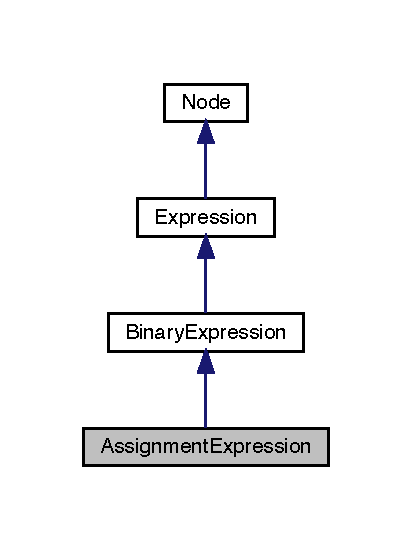
\includegraphics[width=198pt]{struct_assignment_expression__inherit__graph}
\end{center}
\end{figure}


Collaboration diagram for Assignment\+Expression\+:
\nopagebreak
\begin{figure}[H]
\begin{center}
\leavevmode
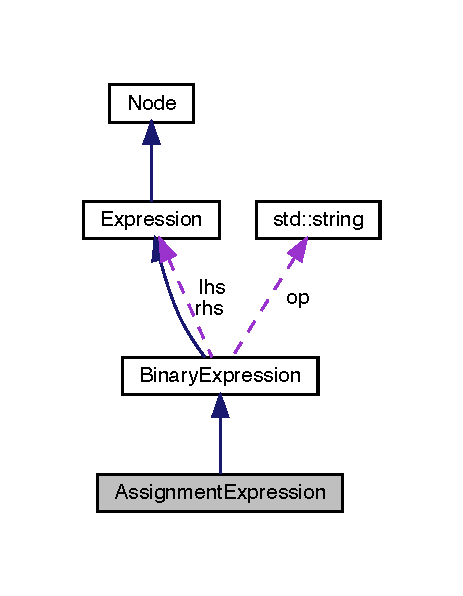
\includegraphics[width=222pt]{struct_assignment_expression__coll__graph}
\end{center}
\end{figure}
\subsection*{Public Member Functions}
\begin{DoxyCompactItemize}
\item 
\hyperlink{struct_assignment_expression_a52c4ebecbb914085110db6fdef413ae6}{Assignment\+Expression} (\textbf{ std\+::string} \hyperlink{struct_binary_expression_a4c33b66e2ffc0a5ede2cdd190bf4bd75}{op}, \hyperlink{struct_expression}{Expression} $\ast$\hyperlink{struct_binary_expression_ae689284a646929c99e634e75f50cb32c}{lhs}=nullptr, \hyperlink{struct_expression}{Expression} $\ast$\hyperlink{struct_binary_expression_ad569ae3b07f428257b0e7a96746ceb32}{rhs}=nullptr)
\item 
void \hyperlink{struct_assignment_expression_ac3d1a00abf176502782937938f629a9f}{accept} (\hyperlink{struct_visitor}{Visitor} \&visitor) const override
\item 
const char $\ast$ \hyperlink{struct_assignment_expression_a9c5da03eec8d7c10f1127ec5029de263}{type} () const override
\end{DoxyCompactItemize}
\subsection*{Additional Inherited Members}


\subsection{Constructor \& Destructor Documentation}
\mbox{\Hypertarget{struct_assignment_expression_a52c4ebecbb914085110db6fdef413ae6}\label{struct_assignment_expression_a52c4ebecbb914085110db6fdef413ae6}} 
\index{Assignment\+Expression@{Assignment\+Expression}!Assignment\+Expression@{Assignment\+Expression}}
\index{Assignment\+Expression@{Assignment\+Expression}!Assignment\+Expression@{Assignment\+Expression}}
\subsubsection{\texorpdfstring{Assignment\+Expression()}{AssignmentExpression()}}
{\footnotesize\ttfamily Assignment\+Expression\+::\+Assignment\+Expression (\begin{DoxyParamCaption}\item[{\textbf{ std\+::string}}]{op,  }\item[{\hyperlink{struct_expression}{Expression} $\ast$}]{lhs = {\ttfamily nullptr},  }\item[{\hyperlink{struct_expression}{Expression} $\ast$}]{rhs = {\ttfamily nullptr} }\end{DoxyParamCaption})\hspace{0.3cm}{\ttfamily [inline]}}



\subsection{Member Function Documentation}
\mbox{\Hypertarget{struct_assignment_expression_ac3d1a00abf176502782937938f629a9f}\label{struct_assignment_expression_ac3d1a00abf176502782937938f629a9f}} 
\index{Assignment\+Expression@{Assignment\+Expression}!accept@{accept}}
\index{accept@{accept}!Assignment\+Expression@{Assignment\+Expression}}
\subsubsection{\texorpdfstring{accept()}{accept()}}
{\footnotesize\ttfamily void Assignment\+Expression\+::accept (\begin{DoxyParamCaption}\item[{\hyperlink{struct_visitor}{Visitor} \&}]{visitor }\end{DoxyParamCaption}) const\hspace{0.3cm}{\ttfamily [inline]}, {\ttfamily [override]}, {\ttfamily [virtual]}}



Reimplemented from \hyperlink{struct_binary_expression_af8318bd8b21b4bbca064e8a6086a10a0}{Binary\+Expression}.

\mbox{\Hypertarget{struct_assignment_expression_a9c5da03eec8d7c10f1127ec5029de263}\label{struct_assignment_expression_a9c5da03eec8d7c10f1127ec5029de263}} 
\index{Assignment\+Expression@{Assignment\+Expression}!type@{type}}
\index{type@{type}!Assignment\+Expression@{Assignment\+Expression}}
\subsubsection{\texorpdfstring{type()}{type()}}
{\footnotesize\ttfamily const char$\ast$ Assignment\+Expression\+::type (\begin{DoxyParamCaption}{ }\end{DoxyParamCaption}) const\hspace{0.3cm}{\ttfamily [inline]}, {\ttfamily [override]}, {\ttfamily [virtual]}}



Reimplemented from \hyperlink{struct_binary_expression_a9ab583e823bac39ed8fd8eb34747ac9f}{Binary\+Expression}.



The documentation for this struct was generated from the following file\+:\begin{DoxyCompactItemize}
\item 
src/\hyperlink{ast_8h}{ast.\+h}\end{DoxyCompactItemize}

\hypertarget{struct_catch_1_1_auto_reg}{}\section{Catch\+:\+:Auto\+Reg Struct Reference}
\label{struct_catch_1_1_auto_reg}\index{Catch\+::\+Auto\+Reg@{Catch\+::\+Auto\+Reg}}


{\ttfamily \#include $<$catch.\+hpp$>$}

\subsection*{Public Member Functions}
\begin{DoxyCompactItemize}
\item 
\hyperlink{struct_catch_1_1_auto_reg_af224f4568d57b8652474df475a164a8c}{Auto\+Reg} (\hyperlink{namespace_catch_a26414f52d0835939fae52aadd27e6257}{Test\+Function} function, \hyperlink{struct_catch_1_1_source_line_info}{Source\+Line\+Info} const \&line\+Info, \hyperlink{struct_catch_1_1_name_and_desc}{Name\+And\+Desc} const \&name\+And\+Desc)
\item 
{\footnotesize template$<$typename C $>$ }\\\hyperlink{struct_catch_1_1_auto_reg_a1bf9207fe0a02b46dc0ab1cc03cbe738}{Auto\+Reg} (void(C\+::$\ast$method)(), char const $\ast$class\+Name, \hyperlink{struct_catch_1_1_name_and_desc}{Name\+And\+Desc} const \&name\+And\+Desc, \hyperlink{struct_catch_1_1_source_line_info}{Source\+Line\+Info} const \&line\+Info)
\item 
\hyperlink{struct_catch_1_1_auto_reg_a3cdb53f1e5ff115310f3372bebe198f1}{$\sim$\+Auto\+Reg} ()
\end{DoxyCompactItemize}


\subsection{Constructor \& Destructor Documentation}
\mbox{\Hypertarget{struct_catch_1_1_auto_reg_af224f4568d57b8652474df475a164a8c}\label{struct_catch_1_1_auto_reg_af224f4568d57b8652474df475a164a8c}} 
\index{Catch\+::\+Auto\+Reg@{Catch\+::\+Auto\+Reg}!Auto\+Reg@{Auto\+Reg}}
\index{Auto\+Reg@{Auto\+Reg}!Catch\+::\+Auto\+Reg@{Catch\+::\+Auto\+Reg}}
\subsubsection{\texorpdfstring{Auto\+Reg()}{AutoReg()}\hspace{0.1cm}{\footnotesize\ttfamily [1/2]}}
{\footnotesize\ttfamily Catch\+::\+Auto\+Reg\+::\+Auto\+Reg (\begin{DoxyParamCaption}\item[{\hyperlink{namespace_catch_a26414f52d0835939fae52aadd27e6257}{Test\+Function}}]{function,  }\item[{\hyperlink{struct_catch_1_1_source_line_info}{Source\+Line\+Info} const \&}]{line\+Info,  }\item[{\hyperlink{struct_catch_1_1_name_and_desc}{Name\+And\+Desc} const \&}]{name\+And\+Desc }\end{DoxyParamCaption})}

\mbox{\Hypertarget{struct_catch_1_1_auto_reg_a1bf9207fe0a02b46dc0ab1cc03cbe738}\label{struct_catch_1_1_auto_reg_a1bf9207fe0a02b46dc0ab1cc03cbe738}} 
\index{Catch\+::\+Auto\+Reg@{Catch\+::\+Auto\+Reg}!Auto\+Reg@{Auto\+Reg}}
\index{Auto\+Reg@{Auto\+Reg}!Catch\+::\+Auto\+Reg@{Catch\+::\+Auto\+Reg}}
\subsubsection{\texorpdfstring{Auto\+Reg()}{AutoReg()}\hspace{0.1cm}{\footnotesize\ttfamily [2/2]}}
{\footnotesize\ttfamily template$<$typename C $>$ \\
Catch\+::\+Auto\+Reg\+::\+Auto\+Reg (\begin{DoxyParamCaption}\item[{void(C\+::$\ast$)()}]{method,  }\item[{char const $\ast$}]{class\+Name,  }\item[{\hyperlink{struct_catch_1_1_name_and_desc}{Name\+And\+Desc} const \&}]{name\+And\+Desc,  }\item[{\hyperlink{struct_catch_1_1_source_line_info}{Source\+Line\+Info} const \&}]{line\+Info }\end{DoxyParamCaption})\hspace{0.3cm}{\ttfamily [inline]}}

\mbox{\Hypertarget{struct_catch_1_1_auto_reg_a3cdb53f1e5ff115310f3372bebe198f1}\label{struct_catch_1_1_auto_reg_a3cdb53f1e5ff115310f3372bebe198f1}} 
\index{Catch\+::\+Auto\+Reg@{Catch\+::\+Auto\+Reg}!````~Auto\+Reg@{$\sim$\+Auto\+Reg}}
\index{````~Auto\+Reg@{$\sim$\+Auto\+Reg}!Catch\+::\+Auto\+Reg@{Catch\+::\+Auto\+Reg}}
\subsubsection{\texorpdfstring{$\sim$\+Auto\+Reg()}{~AutoReg()}}
{\footnotesize\ttfamily Catch\+::\+Auto\+Reg\+::$\sim$\+Auto\+Reg (\begin{DoxyParamCaption}{ }\end{DoxyParamCaption})}



The documentation for this struct was generated from the following file\+:\begin{DoxyCompactItemize}
\item 
src/\hyperlink{catch_8hpp}{catch.\+hpp}\end{DoxyCompactItemize}

\hypertarget{class_basic_lexer}{}\section{Basic\+Lexer$<$ T $>$ Class Template Reference}
\label{class_basic_lexer}\index{Basic\+Lexer$<$ T $>$@{Basic\+Lexer$<$ T $>$}}


{\ttfamily \#include $<$lexer.\+h$>$}



Inheritance diagram for Basic\+Lexer$<$ T $>$\+:\nopagebreak
\begin{figure}[H]
\begin{center}
\leavevmode
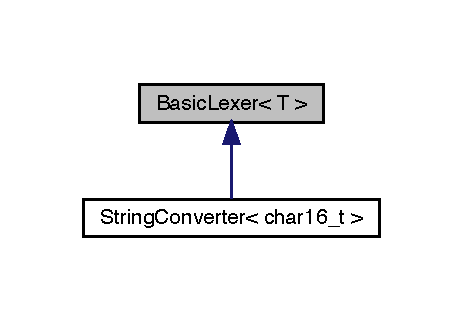
\includegraphics[width=222pt]{class_basic_lexer__inherit__graph}
\end{center}
\end{figure}
\subsection*{Public Member Functions}
\begin{DoxyCompactItemize}
\item 
\hyperlink{class_basic_lexer_abc267aed0ef7227486b932f13b2917f0}{Basic\+Lexer} ()
\item 
\hyperlink{class_basic_lexer_a58d2038fb47025d4e32c20750e713b43}{Basic\+Lexer} (\textbf{ std\+::initializer\+\_\+list}$<$ \hyperlink{class_token}{Token} $>$ \hyperlink{class_basic_lexer_ac20fdf19d5602c563b5cad2bae3ad803}{tokens})
\item 
\hyperlink{class_basic_lexer_a1fd5d2795464497ffbe2bf61c892d619}{Basic\+Lexer} (\textbf{ std\+::vector}$<$ \hyperlink{class_token}{Token} $>$ \hyperlink{class_basic_lexer_ac20fdf19d5602c563b5cad2bae3ad803}{tokens})
\item 
{\footnotesize template$<$typename It $>$ }\\\hyperlink{class_basic_lexer_a7b8cb3ec8ba1ef5567bd280800f891f8}{Basic\+Lexer} (It begin, It end)
\item 
\hyperlink{class_basic_lexer_aee8242905dd2c3541322900bdd05a7b7}{Basic\+Lexer} (const \textbf{ std\+::u16string} \&str)
\item 
\hyperlink{class_basic_lexer_ab486a96453887dc7f9efd08c518ae0b0}{Basic\+Lexer} (const \textbf{ std\+::string} \&str)
\item 
Tokens \hyperlink{class_basic_lexer_ac20fdf19d5602c563b5cad2bae3ad803}{tokens} () const
\end{DoxyCompactItemize}


\subsection{Constructor \& Destructor Documentation}
\mbox{\Hypertarget{class_basic_lexer_abc267aed0ef7227486b932f13b2917f0}\label{class_basic_lexer_abc267aed0ef7227486b932f13b2917f0}} 
\index{Basic\+Lexer@{Basic\+Lexer}!Basic\+Lexer@{Basic\+Lexer}}
\index{Basic\+Lexer@{Basic\+Lexer}!Basic\+Lexer@{Basic\+Lexer}}
\subsubsection{\texorpdfstring{Basic\+Lexer()}{BasicLexer()}\hspace{0.1cm}{\footnotesize\ttfamily [1/6]}}
{\footnotesize\ttfamily template$<$typename T$>$ \\
\hyperlink{class_basic_lexer}{Basic\+Lexer}$<$ T $>$\+::\hyperlink{class_basic_lexer}{Basic\+Lexer} (\begin{DoxyParamCaption}{ }\end{DoxyParamCaption})\hspace{0.3cm}{\ttfamily [inline]}}

\mbox{\Hypertarget{class_basic_lexer_a58d2038fb47025d4e32c20750e713b43}\label{class_basic_lexer_a58d2038fb47025d4e32c20750e713b43}} 
\index{Basic\+Lexer@{Basic\+Lexer}!Basic\+Lexer@{Basic\+Lexer}}
\index{Basic\+Lexer@{Basic\+Lexer}!Basic\+Lexer@{Basic\+Lexer}}
\subsubsection{\texorpdfstring{Basic\+Lexer()}{BasicLexer()}\hspace{0.1cm}{\footnotesize\ttfamily [2/6]}}
{\footnotesize\ttfamily template$<$typename T$>$ \\
\hyperlink{class_basic_lexer}{Basic\+Lexer}$<$ T $>$\+::\hyperlink{class_basic_lexer}{Basic\+Lexer} (\begin{DoxyParamCaption}\item[{\textbf{ std\+::initializer\+\_\+list}$<$ \hyperlink{class_token}{Token} $>$}]{tokens }\end{DoxyParamCaption})\hspace{0.3cm}{\ttfamily [inline]}}

\mbox{\Hypertarget{class_basic_lexer_a1fd5d2795464497ffbe2bf61c892d619}\label{class_basic_lexer_a1fd5d2795464497ffbe2bf61c892d619}} 
\index{Basic\+Lexer@{Basic\+Lexer}!Basic\+Lexer@{Basic\+Lexer}}
\index{Basic\+Lexer@{Basic\+Lexer}!Basic\+Lexer@{Basic\+Lexer}}
\subsubsection{\texorpdfstring{Basic\+Lexer()}{BasicLexer()}\hspace{0.1cm}{\footnotesize\ttfamily [3/6]}}
{\footnotesize\ttfamily template$<$typename T$>$ \\
\hyperlink{class_basic_lexer}{Basic\+Lexer}$<$ T $>$\+::\hyperlink{class_basic_lexer}{Basic\+Lexer} (\begin{DoxyParamCaption}\item[{\textbf{ std\+::vector}$<$ \hyperlink{class_token}{Token} $>$}]{tokens }\end{DoxyParamCaption})\hspace{0.3cm}{\ttfamily [inline]}}

\mbox{\Hypertarget{class_basic_lexer_a7b8cb3ec8ba1ef5567bd280800f891f8}\label{class_basic_lexer_a7b8cb3ec8ba1ef5567bd280800f891f8}} 
\index{Basic\+Lexer@{Basic\+Lexer}!Basic\+Lexer@{Basic\+Lexer}}
\index{Basic\+Lexer@{Basic\+Lexer}!Basic\+Lexer@{Basic\+Lexer}}
\subsubsection{\texorpdfstring{Basic\+Lexer()}{BasicLexer()}\hspace{0.1cm}{\footnotesize\ttfamily [4/6]}}
{\footnotesize\ttfamily template$<$typename T$>$ \\
template$<$typename It $>$ \\
\hyperlink{class_basic_lexer}{Basic\+Lexer}$<$ T $>$\+::\hyperlink{class_basic_lexer}{Basic\+Lexer} (\begin{DoxyParamCaption}\item[{It}]{begin,  }\item[{It}]{end }\end{DoxyParamCaption})\hspace{0.3cm}{\ttfamily [inline]}}

\mbox{\Hypertarget{class_basic_lexer_aee8242905dd2c3541322900bdd05a7b7}\label{class_basic_lexer_aee8242905dd2c3541322900bdd05a7b7}} 
\index{Basic\+Lexer@{Basic\+Lexer}!Basic\+Lexer@{Basic\+Lexer}}
\index{Basic\+Lexer@{Basic\+Lexer}!Basic\+Lexer@{Basic\+Lexer}}
\subsubsection{\texorpdfstring{Basic\+Lexer()}{BasicLexer()}\hspace{0.1cm}{\footnotesize\ttfamily [5/6]}}
{\footnotesize\ttfamily template$<$typename T$>$ \\
\hyperlink{class_basic_lexer}{Basic\+Lexer}$<$ T $>$\+::\hyperlink{class_basic_lexer}{Basic\+Lexer} (\begin{DoxyParamCaption}\item[{const \textbf{ std\+::u16string} \&}]{str }\end{DoxyParamCaption})\hspace{0.3cm}{\ttfamily [inline]}}

\mbox{\Hypertarget{class_basic_lexer_ab486a96453887dc7f9efd08c518ae0b0}\label{class_basic_lexer_ab486a96453887dc7f9efd08c518ae0b0}} 
\index{Basic\+Lexer@{Basic\+Lexer}!Basic\+Lexer@{Basic\+Lexer}}
\index{Basic\+Lexer@{Basic\+Lexer}!Basic\+Lexer@{Basic\+Lexer}}
\subsubsection{\texorpdfstring{Basic\+Lexer()}{BasicLexer()}\hspace{0.1cm}{\footnotesize\ttfamily [6/6]}}
{\footnotesize\ttfamily template$<$typename T$>$ \\
\hyperlink{class_basic_lexer}{Basic\+Lexer}$<$ T $>$\+::\hyperlink{class_basic_lexer}{Basic\+Lexer} (\begin{DoxyParamCaption}\item[{const \textbf{ std\+::string} \&}]{str }\end{DoxyParamCaption})\hspace{0.3cm}{\ttfamily [inline]}}



\subsection{Member Function Documentation}
\mbox{\Hypertarget{class_basic_lexer_ac20fdf19d5602c563b5cad2bae3ad803}\label{class_basic_lexer_ac20fdf19d5602c563b5cad2bae3ad803}} 
\index{Basic\+Lexer@{Basic\+Lexer}!tokens@{tokens}}
\index{tokens@{tokens}!Basic\+Lexer@{Basic\+Lexer}}
\subsubsection{\texorpdfstring{tokens()}{tokens()}}
{\footnotesize\ttfamily template$<$typename T$>$ \\
Tokens \hyperlink{class_basic_lexer}{Basic\+Lexer}$<$ T $>$\+::tokens (\begin{DoxyParamCaption}{ }\end{DoxyParamCaption}) const\hspace{0.3cm}{\ttfamily [inline]}}



The documentation for this class was generated from the following file\+:\begin{DoxyCompactItemize}
\item 
src/\hyperlink{lexer_8h}{lexer.\+h}\end{DoxyCompactItemize}

\hypertarget{struct_basic_visitor}{}\section{Basic\+Visitor Struct Reference}
\label{struct_basic_visitor}\index{Basic\+Visitor@{Basic\+Visitor}}


{\ttfamily \#include $<$basic\+\_\+visitor.\+h$>$}



Inheritance diagram for Basic\+Visitor\+:\nopagebreak
\begin{figure}[H]
\begin{center}
\leavevmode
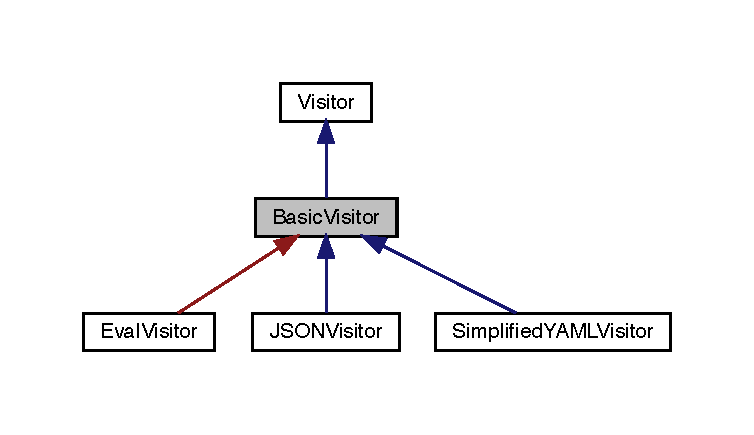
\includegraphics[width=350pt]{struct_basic_visitor__inherit__graph}
\end{center}
\end{figure}


Collaboration diagram for Basic\+Visitor\+:\nopagebreak
\begin{figure}[H]
\begin{center}
\leavevmode
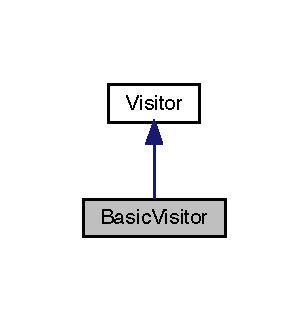
\includegraphics[width=148pt]{struct_basic_visitor__coll__graph}
\end{center}
\end{figure}
\subsection*{Public Member Functions}
\begin{DoxyCompactItemize}
\item 
{\footnotesize template$<$typename T $>$ }\\void \hyperlink{struct_basic_visitor_aef8aa82a7e5149b6153f097af8daa647}{apply\+\_\+impl} (const T $\ast$node)
\item 
{\footnotesize template$<$typename T $>$ }\\void \hyperlink{struct_basic_visitor_a128388a75069690c9c108ce87b69cde8}{apply\+\_\+impl} (const \textbf{ std\+::vector}$<$ T $>$ \&list)
\item 
{\footnotesize template$<$typename... Args$>$ }\\void \hyperlink{struct_basic_visitor_a85afee760b9e02733ed01ff56a96f09c}{apply} (Args \&\&... args)
\item 
void \hyperlink{struct_basic_visitor_a15fc407e84d51dad443c3b7e135302ae}{operator()} (const \hyperlink{struct_this}{This} \&) override
\item 
void \hyperlink{struct_basic_visitor_ac9ae9d17e262b8c71696d978be89af4d}{operator()} (const \hyperlink{struct_identifier}{Identifier} \&) override
\item 
void \hyperlink{struct_basic_visitor_afc1fe7c3d76c98c6d489d98c66d773de}{operator()} (const \hyperlink{struct_null_literal}{Null\+Literal} \&) override
\item 
void \hyperlink{struct_basic_visitor_a2971ac256de1c7b0206b44f888d9abd5}{operator()} (const \hyperlink{struct_boolean_literal}{Boolean\+Literal} \&) override
\item 
void \hyperlink{struct_basic_visitor_a177e744fc03783b7fbb83d3292a7c029}{operator()} (const \hyperlink{struct_numeric_literal}{Numeric\+Literal} \&) override
\item 
void \hyperlink{struct_basic_visitor_a1e22bd82234168dd70579eabe84574ad}{operator()} (const \hyperlink{struct_string_literal}{String\+Literal} \&) override
\item 
void \hyperlink{struct_basic_visitor_a40d181efc4db66a595baaee6e78c65db}{operator()} (const \hyperlink{struct_regular_expression_literal}{Regular\+Expression\+Literal} \&) override
\item 
void \hyperlink{struct_basic_visitor_a0f625d975e964cda064bbc0f12f97558}{operator()} (const \hyperlink{struct_array_literal}{Array\+Literal} \&node) override
\item 
void \hyperlink{struct_basic_visitor_a1f0d676e1575a8efa7fd7149ef9d93be}{operator()} (const \hyperlink{struct_object_literal}{Object\+Literal} \&node) override
\item 
void \hyperlink{struct_basic_visitor_aa3811d723e70227de815461380d861c9}{operator()} (const \hyperlink{struct_this_expression}{This\+Expression} \&) override
\item 
void \hyperlink{struct_basic_visitor_a453bc258129808d4e1e1efefcfa893a0}{operator()} (const \hyperlink{struct_identifier_expression}{Identifier\+Expression} \&node) override
\item 
void \hyperlink{struct_basic_visitor_af86e1dfc1fb346b3dd94a63b6017f4d4}{operator()} (const \hyperlink{struct_literal_expression}{Literal\+Expression} \&node) override
\item 
void \hyperlink{struct_basic_visitor_a1b0936671dd80c4e4ce029e41b216ba6}{operator()} (const \hyperlink{struct_array_expression}{Array\+Expression} \&node) override
\item 
void \hyperlink{struct_basic_visitor_a2bdc5b88714c947eb15d5530240c660c}{operator()} (const \hyperlink{struct_object_expression}{Object\+Expression} \&node) override
\item 
void \hyperlink{struct_basic_visitor_a74c4ab927dc2907784f886245a29296b}{operator()} (const \hyperlink{struct_member_expression}{Member\+Expression} \&node) override
\item 
void \hyperlink{struct_basic_visitor_ab73b6e87ae7344434aa833bd93f4480b}{operator()} (const \hyperlink{struct_new_expression}{New\+Expression} \&node) override
\item 
void \hyperlink{struct_basic_visitor_a455b2414d59a21bae802bd8b20544252}{operator()} (const \hyperlink{struct_call_expression}{Call\+Expression} \&node) override
\item 
void \hyperlink{struct_basic_visitor_ac7e33b8e36fa46d32e3cf517bf9de9bb}{operator()} (const \hyperlink{struct_postfix_expression}{Postfix\+Expression} \&node) override
\item 
void \hyperlink{struct_basic_visitor_a3ae4c9623d2f589f6f026833a7c1dd13}{operator()} (const \hyperlink{struct_unary_expression}{Unary\+Expression} \&node) override
\item 
void \hyperlink{struct_basic_visitor_a9433a6a9dcdd64f97ea1c392208a3305}{operator()} (const \hyperlink{struct_binary_expression}{Binary\+Expression} \&node) override
\item 
void \hyperlink{struct_basic_visitor_ab121f54f6337dc726745c65f47812d8d}{operator()} (const \hyperlink{struct_conditional_expression}{Conditional\+Expression} \&node) override
\item 
void \hyperlink{struct_basic_visitor_a8b5be95fdf83d05891a738923bace2be}{operator()} (const \hyperlink{struct_assignment_expression}{Assignment\+Expression} \&node) override
\item 
void \hyperlink{struct_basic_visitor_ae6e86620ac38764d055615b005b7a1d4}{operator()} (const \hyperlink{struct_function_expression}{Function\+Expression} \&node) override
\item 
void \hyperlink{struct_basic_visitor_a6ab713b4b992eb420c89a2326e351fd3}{operator()} (const \hyperlink{struct_block}{Block} \&node) override
\item 
void \hyperlink{struct_basic_visitor_afb110c94ddb7c8383f03541c76ff8bf7}{operator()} (const \hyperlink{struct_variable_statement}{Variable\+Statement} \&stmt) override
\item 
void \hyperlink{struct_basic_visitor_a99efd6097eb643d8738f1bb42f51f17e}{operator()} (const \hyperlink{struct_empty_statement}{Empty\+Statement} \&) override
\item 
void \hyperlink{struct_basic_visitor_a6c369f60a28dffd5149258e32a81cb6e}{operator()} (const \hyperlink{struct_expression_statement}{Expression\+Statement} \&stmt) override
\item 
void \hyperlink{struct_basic_visitor_a4d4e3621e47ea469c0e59d0b1c6c657b}{operator()} (const \hyperlink{struct_if_statement}{If\+Statement} \&stmt) override
\item 
void \hyperlink{struct_basic_visitor_a51de918d2508db22dba21233582f670e}{operator()} (const \hyperlink{struct_do_while_statement}{Do\+While\+Statement} \&) override
\item 
void \hyperlink{struct_basic_visitor_a0a7f4e29df8d0725070caa8560d4c4b5}{operator()} (const \hyperlink{struct_while_statement}{While\+Statement} \&) override
\item 
void \hyperlink{struct_basic_visitor_a62043123e2fb7e0c22229b0e5bb7dcc8}{operator()} (const \hyperlink{struct_for_statement}{For\+Statement} \&) override
\item 
void \hyperlink{struct_basic_visitor_abfa9eb036c3927634be4aef270579672}{operator()} (const \hyperlink{struct_for_in_statement}{For\+In\+Statement} \&) override
\item 
void \hyperlink{struct_basic_visitor_a5614facf759b3aa15b518df911cd9a6c}{operator()} (const \hyperlink{struct_continue_statement}{Continue\+Statement} \&stmt) override
\item 
void \hyperlink{struct_basic_visitor_ae0ecf9dc46dc7654488a1b2002dceb25}{operator()} (const \hyperlink{struct_break_statement}{Break\+Statement} \&stmt) override
\item 
void \hyperlink{struct_basic_visitor_ac7a0c630d96799333d3d32c8ca465f51}{operator()} (const \hyperlink{struct_return_statement}{Return\+Statement} \&stmt) override
\item 
void \hyperlink{struct_basic_visitor_a3dafb609d4df2fa786f7fe4fb25f1b9d}{operator()} (const \hyperlink{struct_with_statement}{With\+Statement} \&stmt) override
\item 
void \hyperlink{struct_basic_visitor_ae53f4199cddb021c0f30f898796942c4}{operator()} (const \hyperlink{struct_labelled_statement}{Labelled\+Statement} \&stmt) override
\item 
void \hyperlink{struct_basic_visitor_af97609b1ab2068d18ea5e94240819ccb}{operator()} (const \hyperlink{struct_switch_statement}{Switch\+Statement} \&stmt) override
\item 
void \hyperlink{struct_basic_visitor_a19c4ebe7b4d6d1cbddc354cf8e8267e4}{operator()} (const \hyperlink{struct_throw_statement}{Throw\+Statement} \&stmt) override
\item 
void \hyperlink{struct_basic_visitor_a2b4e8d7c1f46d71adbc8bf2f4b597fcc}{operator()} (const \hyperlink{struct_try_statement}{Try\+Statement} \&stmt) override
\item 
void \hyperlink{struct_basic_visitor_a193c296097cb56beab2cc74165668df8}{operator()} (const \hyperlink{struct_debugger_statement}{Debugger\+Statement} \&) override
\item 
void \hyperlink{struct_basic_visitor_ae3d4b26dfc7eaae787a33d9e1e73bc2e}{operator()} (const \hyperlink{struct_case_clause}{Case\+Clause} \&node) override
\item 
void \hyperlink{struct_basic_visitor_ae0235e556d05ba170398dcd7f0c25cb1}{operator()} (const \hyperlink{struct_default_clause}{Default\+Clause} \&node) override
\item 
void \hyperlink{struct_basic_visitor_a2871985a62b51f8f5212a5a65e47b7b8}{operator()} (const \hyperlink{struct_function_declaration}{Function\+Declaration} \&decl) override
\item 
void \hyperlink{struct_basic_visitor_ac9435a48d44ce32bd726cbf46bcc9032}{operator()} (const \hyperlink{struct_function_body}{Function\+Body} \&node) override
\item 
void \hyperlink{struct_basic_visitor_a0405c0df4a21c4735feaa98f5cd0cfa9}{operator()} (const \hyperlink{struct_variable_declaration}{Variable\+Declaration} \&decl) override
\item 
void \hyperlink{struct_basic_visitor_af64d7b88cbffe3d0717e9607704f56da}{operator()} (const \hyperlink{struct_elision}{Elision} \&) override
\item 
void \hyperlink{struct_basic_visitor_a4e82e722dc7c0cc04b1a39e0961b29f6}{operator()} (const \hyperlink{struct_property_name}{Property\+Name} \&) override
\item 
void \hyperlink{struct_basic_visitor_a3a868dc82a76118467f3a1ae4b1c92cd}{operator()} (const \hyperlink{struct_property_assignment}{Property\+Assignment} \&node) override
\item 
void \hyperlink{struct_basic_visitor_a8fecced7470cc28d2294c93e7df7ac1d}{operator()} (const \hyperlink{struct_arguments}{Arguments} \&node) override
\item 
void \hyperlink{struct_basic_visitor_adeaf13cc53c36c871d89d6f42a1ec8db}{operator()} (const \hyperlink{struct_program}{Program} \&node) override
\item 
void \hyperlink{struct_basic_visitor_a365071938626ac065ac413ba0e6d382f}{operator()} (const \hyperlink{struct_program_declaration}{Program\+Declaration} \&decl) override
\item 
void \hyperlink{struct_basic_visitor_ae04e6bd948d2f85acaff8744ad6ab0d7}{operator()} (const \hyperlink{struct_element_list}{Element\+List} \&list) override
\item 
void \hyperlink{struct_basic_visitor_a1cae5b2aa57d5214a6e89f6368ae5be1}{operator()} (const \hyperlink{struct_property_name_and_value_list}{Property\+Name\+And\+Value\+List} \&list) override
\item 
void \hyperlink{struct_basic_visitor_a3ebaf2b9a8a274df6d9960f1d6d8b6a6}{operator()} (const \hyperlink{struct_argument_list}{Argument\+List} \&list) override
\item 
void \hyperlink{struct_basic_visitor_aa04dfa4159f7711dcfd3d85ffab8ae88}{operator()} (const \hyperlink{struct_variable_declaration_list}{Variable\+Declaration\+List} \&list) override
\item 
void \hyperlink{struct_basic_visitor_a253a7061c246597f81f1122988704345}{operator()} (const \hyperlink{struct_statement_list}{Statement\+List} \&list) override
\item 
void \hyperlink{struct_basic_visitor_af108c842c7b483b2cb544dd77b171486}{operator()} (const \hyperlink{struct_case_block}{Case\+Block} \&list) override
\item 
void \hyperlink{struct_basic_visitor_a4cb8f522aa48db2270e3af61ee7b3370}{operator()} (const \hyperlink{struct_source_elements}{Source\+Elements} \&list) override
\item 
void \hyperlink{struct_basic_visitor_a3ce54960164c84e8d61c4c710362d6e3}{operator()} (const \hyperlink{struct_formal_parameter_list}{Formal\+Parameter\+List} \&list) override
\end{DoxyCompactItemize}


\subsection{Member Function Documentation}
\mbox{\Hypertarget{struct_basic_visitor_a85afee760b9e02733ed01ff56a96f09c}\label{struct_basic_visitor_a85afee760b9e02733ed01ff56a96f09c}} 
\index{Basic\+Visitor@{Basic\+Visitor}!apply@{apply}}
\index{apply@{apply}!Basic\+Visitor@{Basic\+Visitor}}
\subsubsection{\texorpdfstring{apply()}{apply()}}
{\footnotesize\ttfamily template$<$typename... Args$>$ \\
void Basic\+Visitor\+::apply (\begin{DoxyParamCaption}\item[{Args \&\&...}]{args }\end{DoxyParamCaption})\hspace{0.3cm}{\ttfamily [inline]}}

\mbox{\Hypertarget{struct_basic_visitor_aef8aa82a7e5149b6153f097af8daa647}\label{struct_basic_visitor_aef8aa82a7e5149b6153f097af8daa647}} 
\index{Basic\+Visitor@{Basic\+Visitor}!apply\+\_\+impl@{apply\+\_\+impl}}
\index{apply\+\_\+impl@{apply\+\_\+impl}!Basic\+Visitor@{Basic\+Visitor}}
\subsubsection{\texorpdfstring{apply\+\_\+impl()}{apply\_impl()}\hspace{0.1cm}{\footnotesize\ttfamily [1/2]}}
{\footnotesize\ttfamily template$<$typename T $>$ \\
void Basic\+Visitor\+::apply\+\_\+impl (\begin{DoxyParamCaption}\item[{const T $\ast$}]{node }\end{DoxyParamCaption})\hspace{0.3cm}{\ttfamily [inline]}}

\mbox{\Hypertarget{struct_basic_visitor_a128388a75069690c9c108ce87b69cde8}\label{struct_basic_visitor_a128388a75069690c9c108ce87b69cde8}} 
\index{Basic\+Visitor@{Basic\+Visitor}!apply\+\_\+impl@{apply\+\_\+impl}}
\index{apply\+\_\+impl@{apply\+\_\+impl}!Basic\+Visitor@{Basic\+Visitor}}
\subsubsection{\texorpdfstring{apply\+\_\+impl()}{apply\_impl()}\hspace{0.1cm}{\footnotesize\ttfamily [2/2]}}
{\footnotesize\ttfamily template$<$typename T $>$ \\
void Basic\+Visitor\+::apply\+\_\+impl (\begin{DoxyParamCaption}\item[{const \textbf{ std\+::vector}$<$ T $>$ \&}]{list }\end{DoxyParamCaption})\hspace{0.3cm}{\ttfamily [inline]}}

\mbox{\Hypertarget{struct_basic_visitor_a15fc407e84d51dad443c3b7e135302ae}\label{struct_basic_visitor_a15fc407e84d51dad443c3b7e135302ae}} 
\index{Basic\+Visitor@{Basic\+Visitor}!operator()@{operator()}}
\index{operator()@{operator()}!Basic\+Visitor@{Basic\+Visitor}}
\subsubsection{\texorpdfstring{operator()()}{operator()()}\hspace{0.1cm}{\footnotesize\ttfamily [1/60]}}
{\footnotesize\ttfamily void Basic\+Visitor\+::operator() (\begin{DoxyParamCaption}\item[{const \hyperlink{struct_this}{This} \&}]{ }\end{DoxyParamCaption})\hspace{0.3cm}{\ttfamily [inline]}, {\ttfamily [override]}, {\ttfamily [virtual]}}



Implements \hyperlink{struct_visitor_a7a043c9da4e7f8233db48afb82dbc7bc}{Visitor}.

\mbox{\Hypertarget{struct_basic_visitor_ac9ae9d17e262b8c71696d978be89af4d}\label{struct_basic_visitor_ac9ae9d17e262b8c71696d978be89af4d}} 
\index{Basic\+Visitor@{Basic\+Visitor}!operator()@{operator()}}
\index{operator()@{operator()}!Basic\+Visitor@{Basic\+Visitor}}
\subsubsection{\texorpdfstring{operator()()}{operator()()}\hspace{0.1cm}{\footnotesize\ttfamily [2/60]}}
{\footnotesize\ttfamily void Basic\+Visitor\+::operator() (\begin{DoxyParamCaption}\item[{const \hyperlink{struct_identifier}{Identifier} \&}]{ }\end{DoxyParamCaption})\hspace{0.3cm}{\ttfamily [inline]}, {\ttfamily [override]}, {\ttfamily [virtual]}}



Implements \hyperlink{struct_visitor_a2d09687aa24b1b618c6205f8413c2dd3}{Visitor}.

\mbox{\Hypertarget{struct_basic_visitor_afc1fe7c3d76c98c6d489d98c66d773de}\label{struct_basic_visitor_afc1fe7c3d76c98c6d489d98c66d773de}} 
\index{Basic\+Visitor@{Basic\+Visitor}!operator()@{operator()}}
\index{operator()@{operator()}!Basic\+Visitor@{Basic\+Visitor}}
\subsubsection{\texorpdfstring{operator()()}{operator()()}\hspace{0.1cm}{\footnotesize\ttfamily [3/60]}}
{\footnotesize\ttfamily void Basic\+Visitor\+::operator() (\begin{DoxyParamCaption}\item[{const \hyperlink{struct_null_literal}{Null\+Literal} \&}]{ }\end{DoxyParamCaption})\hspace{0.3cm}{\ttfamily [inline]}, {\ttfamily [override]}, {\ttfamily [virtual]}}



Implements \hyperlink{struct_visitor_a2278ee24407bdc0d3addf887754d4c6c}{Visitor}.

\mbox{\Hypertarget{struct_basic_visitor_a2971ac256de1c7b0206b44f888d9abd5}\label{struct_basic_visitor_a2971ac256de1c7b0206b44f888d9abd5}} 
\index{Basic\+Visitor@{Basic\+Visitor}!operator()@{operator()}}
\index{operator()@{operator()}!Basic\+Visitor@{Basic\+Visitor}}
\subsubsection{\texorpdfstring{operator()()}{operator()()}\hspace{0.1cm}{\footnotesize\ttfamily [4/60]}}
{\footnotesize\ttfamily void Basic\+Visitor\+::operator() (\begin{DoxyParamCaption}\item[{const \hyperlink{struct_boolean_literal}{Boolean\+Literal} \&}]{ }\end{DoxyParamCaption})\hspace{0.3cm}{\ttfamily [inline]}, {\ttfamily [override]}, {\ttfamily [virtual]}}



Implements \hyperlink{struct_visitor_af3b394eaf1b9b1db22379aedcb234a2f}{Visitor}.

\mbox{\Hypertarget{struct_basic_visitor_a177e744fc03783b7fbb83d3292a7c029}\label{struct_basic_visitor_a177e744fc03783b7fbb83d3292a7c029}} 
\index{Basic\+Visitor@{Basic\+Visitor}!operator()@{operator()}}
\index{operator()@{operator()}!Basic\+Visitor@{Basic\+Visitor}}
\subsubsection{\texorpdfstring{operator()()}{operator()()}\hspace{0.1cm}{\footnotesize\ttfamily [5/60]}}
{\footnotesize\ttfamily void Basic\+Visitor\+::operator() (\begin{DoxyParamCaption}\item[{const \hyperlink{struct_numeric_literal}{Numeric\+Literal} \&}]{ }\end{DoxyParamCaption})\hspace{0.3cm}{\ttfamily [inline]}, {\ttfamily [override]}, {\ttfamily [virtual]}}



Implements \hyperlink{struct_visitor_a6d707fe0c1563b39aae3ecd7ddb5ab8f}{Visitor}.

\mbox{\Hypertarget{struct_basic_visitor_a1e22bd82234168dd70579eabe84574ad}\label{struct_basic_visitor_a1e22bd82234168dd70579eabe84574ad}} 
\index{Basic\+Visitor@{Basic\+Visitor}!operator()@{operator()}}
\index{operator()@{operator()}!Basic\+Visitor@{Basic\+Visitor}}
\subsubsection{\texorpdfstring{operator()()}{operator()()}\hspace{0.1cm}{\footnotesize\ttfamily [6/60]}}
{\footnotesize\ttfamily void Basic\+Visitor\+::operator() (\begin{DoxyParamCaption}\item[{const \hyperlink{struct_string_literal}{String\+Literal} \&}]{ }\end{DoxyParamCaption})\hspace{0.3cm}{\ttfamily [inline]}, {\ttfamily [override]}, {\ttfamily [virtual]}}



Implements \hyperlink{struct_visitor_a6bab8ba66edf0cc73cb92073269e7848}{Visitor}.

\mbox{\Hypertarget{struct_basic_visitor_a40d181efc4db66a595baaee6e78c65db}\label{struct_basic_visitor_a40d181efc4db66a595baaee6e78c65db}} 
\index{Basic\+Visitor@{Basic\+Visitor}!operator()@{operator()}}
\index{operator()@{operator()}!Basic\+Visitor@{Basic\+Visitor}}
\subsubsection{\texorpdfstring{operator()()}{operator()()}\hspace{0.1cm}{\footnotesize\ttfamily [7/60]}}
{\footnotesize\ttfamily void Basic\+Visitor\+::operator() (\begin{DoxyParamCaption}\item[{const \hyperlink{struct_regular_expression_literal}{Regular\+Expression\+Literal} \&}]{ }\end{DoxyParamCaption})\hspace{0.3cm}{\ttfamily [inline]}, {\ttfamily [override]}, {\ttfamily [virtual]}}



Implements \hyperlink{struct_visitor_aea90f9399628f301f8c25a62ce268097}{Visitor}.

\mbox{\Hypertarget{struct_basic_visitor_a0f625d975e964cda064bbc0f12f97558}\label{struct_basic_visitor_a0f625d975e964cda064bbc0f12f97558}} 
\index{Basic\+Visitor@{Basic\+Visitor}!operator()@{operator()}}
\index{operator()@{operator()}!Basic\+Visitor@{Basic\+Visitor}}
\subsubsection{\texorpdfstring{operator()()}{operator()()}\hspace{0.1cm}{\footnotesize\ttfamily [8/60]}}
{\footnotesize\ttfamily void Basic\+Visitor\+::operator() (\begin{DoxyParamCaption}\item[{const \hyperlink{struct_array_literal}{Array\+Literal} \&}]{node }\end{DoxyParamCaption})\hspace{0.3cm}{\ttfamily [inline]}, {\ttfamily [override]}, {\ttfamily [virtual]}}



Implements \hyperlink{struct_visitor_a46f9846468f2c12ddc585cfe0421e6f0}{Visitor}.

\mbox{\Hypertarget{struct_basic_visitor_a1f0d676e1575a8efa7fd7149ef9d93be}\label{struct_basic_visitor_a1f0d676e1575a8efa7fd7149ef9d93be}} 
\index{Basic\+Visitor@{Basic\+Visitor}!operator()@{operator()}}
\index{operator()@{operator()}!Basic\+Visitor@{Basic\+Visitor}}
\subsubsection{\texorpdfstring{operator()()}{operator()()}\hspace{0.1cm}{\footnotesize\ttfamily [9/60]}}
{\footnotesize\ttfamily void Basic\+Visitor\+::operator() (\begin{DoxyParamCaption}\item[{const \hyperlink{struct_object_literal}{Object\+Literal} \&}]{node }\end{DoxyParamCaption})\hspace{0.3cm}{\ttfamily [inline]}, {\ttfamily [override]}, {\ttfamily [virtual]}}



Implements \hyperlink{struct_visitor_ad85d9aa9718801a1a8233cf51d8f7055}{Visitor}.

\mbox{\Hypertarget{struct_basic_visitor_aa3811d723e70227de815461380d861c9}\label{struct_basic_visitor_aa3811d723e70227de815461380d861c9}} 
\index{Basic\+Visitor@{Basic\+Visitor}!operator()@{operator()}}
\index{operator()@{operator()}!Basic\+Visitor@{Basic\+Visitor}}
\subsubsection{\texorpdfstring{operator()()}{operator()()}\hspace{0.1cm}{\footnotesize\ttfamily [10/60]}}
{\footnotesize\ttfamily void Basic\+Visitor\+::operator() (\begin{DoxyParamCaption}\item[{const \hyperlink{struct_this_expression}{This\+Expression} \&}]{ }\end{DoxyParamCaption})\hspace{0.3cm}{\ttfamily [inline]}, {\ttfamily [override]}, {\ttfamily [virtual]}}



Implements \hyperlink{struct_visitor_ae8eb5856c0ed7ff4840fa9045c886f59}{Visitor}.

\mbox{\Hypertarget{struct_basic_visitor_a453bc258129808d4e1e1efefcfa893a0}\label{struct_basic_visitor_a453bc258129808d4e1e1efefcfa893a0}} 
\index{Basic\+Visitor@{Basic\+Visitor}!operator()@{operator()}}
\index{operator()@{operator()}!Basic\+Visitor@{Basic\+Visitor}}
\subsubsection{\texorpdfstring{operator()()}{operator()()}\hspace{0.1cm}{\footnotesize\ttfamily [11/60]}}
{\footnotesize\ttfamily void Basic\+Visitor\+::operator() (\begin{DoxyParamCaption}\item[{const \hyperlink{struct_identifier_expression}{Identifier\+Expression} \&}]{node }\end{DoxyParamCaption})\hspace{0.3cm}{\ttfamily [inline]}, {\ttfamily [override]}, {\ttfamily [virtual]}}



Implements \hyperlink{struct_visitor_ad804ffa8c84a6fa58b18980cd3ec71af}{Visitor}.

\mbox{\Hypertarget{struct_basic_visitor_af86e1dfc1fb346b3dd94a63b6017f4d4}\label{struct_basic_visitor_af86e1dfc1fb346b3dd94a63b6017f4d4}} 
\index{Basic\+Visitor@{Basic\+Visitor}!operator()@{operator()}}
\index{operator()@{operator()}!Basic\+Visitor@{Basic\+Visitor}}
\subsubsection{\texorpdfstring{operator()()}{operator()()}\hspace{0.1cm}{\footnotesize\ttfamily [12/60]}}
{\footnotesize\ttfamily void Basic\+Visitor\+::operator() (\begin{DoxyParamCaption}\item[{const \hyperlink{struct_literal_expression}{Literal\+Expression} \&}]{node }\end{DoxyParamCaption})\hspace{0.3cm}{\ttfamily [inline]}, {\ttfamily [override]}, {\ttfamily [virtual]}}



Implements \hyperlink{struct_visitor_a4f9ed19fc09fb7f31e8af350d028a5fd}{Visitor}.

\mbox{\Hypertarget{struct_basic_visitor_a1b0936671dd80c4e4ce029e41b216ba6}\label{struct_basic_visitor_a1b0936671dd80c4e4ce029e41b216ba6}} 
\index{Basic\+Visitor@{Basic\+Visitor}!operator()@{operator()}}
\index{operator()@{operator()}!Basic\+Visitor@{Basic\+Visitor}}
\subsubsection{\texorpdfstring{operator()()}{operator()()}\hspace{0.1cm}{\footnotesize\ttfamily [13/60]}}
{\footnotesize\ttfamily void Basic\+Visitor\+::operator() (\begin{DoxyParamCaption}\item[{const \hyperlink{struct_array_expression}{Array\+Expression} \&}]{node }\end{DoxyParamCaption})\hspace{0.3cm}{\ttfamily [inline]}, {\ttfamily [override]}, {\ttfamily [virtual]}}



Implements \hyperlink{struct_visitor_a99d582c067b225f1022a27c44beb801c}{Visitor}.

\mbox{\Hypertarget{struct_basic_visitor_a2bdc5b88714c947eb15d5530240c660c}\label{struct_basic_visitor_a2bdc5b88714c947eb15d5530240c660c}} 
\index{Basic\+Visitor@{Basic\+Visitor}!operator()@{operator()}}
\index{operator()@{operator()}!Basic\+Visitor@{Basic\+Visitor}}
\subsubsection{\texorpdfstring{operator()()}{operator()()}\hspace{0.1cm}{\footnotesize\ttfamily [14/60]}}
{\footnotesize\ttfamily void Basic\+Visitor\+::operator() (\begin{DoxyParamCaption}\item[{const \hyperlink{struct_object_expression}{Object\+Expression} \&}]{node }\end{DoxyParamCaption})\hspace{0.3cm}{\ttfamily [inline]}, {\ttfamily [override]}, {\ttfamily [virtual]}}



Implements \hyperlink{struct_visitor_a58d0e4e708057211465ba14290a0a154}{Visitor}.

\mbox{\Hypertarget{struct_basic_visitor_a74c4ab927dc2907784f886245a29296b}\label{struct_basic_visitor_a74c4ab927dc2907784f886245a29296b}} 
\index{Basic\+Visitor@{Basic\+Visitor}!operator()@{operator()}}
\index{operator()@{operator()}!Basic\+Visitor@{Basic\+Visitor}}
\subsubsection{\texorpdfstring{operator()()}{operator()()}\hspace{0.1cm}{\footnotesize\ttfamily [15/60]}}
{\footnotesize\ttfamily void Basic\+Visitor\+::operator() (\begin{DoxyParamCaption}\item[{const \hyperlink{struct_member_expression}{Member\+Expression} \&}]{node }\end{DoxyParamCaption})\hspace{0.3cm}{\ttfamily [inline]}, {\ttfamily [override]}, {\ttfamily [virtual]}}



Implements \hyperlink{struct_visitor_a175fd29619240cc378703de4c357f348}{Visitor}.

\mbox{\Hypertarget{struct_basic_visitor_ab73b6e87ae7344434aa833bd93f4480b}\label{struct_basic_visitor_ab73b6e87ae7344434aa833bd93f4480b}} 
\index{Basic\+Visitor@{Basic\+Visitor}!operator()@{operator()}}
\index{operator()@{operator()}!Basic\+Visitor@{Basic\+Visitor}}
\subsubsection{\texorpdfstring{operator()()}{operator()()}\hspace{0.1cm}{\footnotesize\ttfamily [16/60]}}
{\footnotesize\ttfamily void Basic\+Visitor\+::operator() (\begin{DoxyParamCaption}\item[{const \hyperlink{struct_new_expression}{New\+Expression} \&}]{node }\end{DoxyParamCaption})\hspace{0.3cm}{\ttfamily [inline]}, {\ttfamily [override]}, {\ttfamily [virtual]}}



Implements \hyperlink{struct_visitor_a13ead8d5ef82f284e301ba8127e9fb56}{Visitor}.

\mbox{\Hypertarget{struct_basic_visitor_a455b2414d59a21bae802bd8b20544252}\label{struct_basic_visitor_a455b2414d59a21bae802bd8b20544252}} 
\index{Basic\+Visitor@{Basic\+Visitor}!operator()@{operator()}}
\index{operator()@{operator()}!Basic\+Visitor@{Basic\+Visitor}}
\subsubsection{\texorpdfstring{operator()()}{operator()()}\hspace{0.1cm}{\footnotesize\ttfamily [17/60]}}
{\footnotesize\ttfamily void Basic\+Visitor\+::operator() (\begin{DoxyParamCaption}\item[{const \hyperlink{struct_call_expression}{Call\+Expression} \&}]{node }\end{DoxyParamCaption})\hspace{0.3cm}{\ttfamily [inline]}, {\ttfamily [override]}, {\ttfamily [virtual]}}



Implements \hyperlink{struct_visitor_aa6152c6f355690fd1c4db37fff303614}{Visitor}.

\mbox{\Hypertarget{struct_basic_visitor_ac7e33b8e36fa46d32e3cf517bf9de9bb}\label{struct_basic_visitor_ac7e33b8e36fa46d32e3cf517bf9de9bb}} 
\index{Basic\+Visitor@{Basic\+Visitor}!operator()@{operator()}}
\index{operator()@{operator()}!Basic\+Visitor@{Basic\+Visitor}}
\subsubsection{\texorpdfstring{operator()()}{operator()()}\hspace{0.1cm}{\footnotesize\ttfamily [18/60]}}
{\footnotesize\ttfamily void Basic\+Visitor\+::operator() (\begin{DoxyParamCaption}\item[{const \hyperlink{struct_postfix_expression}{Postfix\+Expression} \&}]{node }\end{DoxyParamCaption})\hspace{0.3cm}{\ttfamily [inline]}, {\ttfamily [override]}, {\ttfamily [virtual]}}



Implements \hyperlink{struct_visitor_acd630c29940c6785726ce51c7db0aab9}{Visitor}.

\mbox{\Hypertarget{struct_basic_visitor_a3ae4c9623d2f589f6f026833a7c1dd13}\label{struct_basic_visitor_a3ae4c9623d2f589f6f026833a7c1dd13}} 
\index{Basic\+Visitor@{Basic\+Visitor}!operator()@{operator()}}
\index{operator()@{operator()}!Basic\+Visitor@{Basic\+Visitor}}
\subsubsection{\texorpdfstring{operator()()}{operator()()}\hspace{0.1cm}{\footnotesize\ttfamily [19/60]}}
{\footnotesize\ttfamily void Basic\+Visitor\+::operator() (\begin{DoxyParamCaption}\item[{const \hyperlink{struct_unary_expression}{Unary\+Expression} \&}]{node }\end{DoxyParamCaption})\hspace{0.3cm}{\ttfamily [inline]}, {\ttfamily [override]}, {\ttfamily [virtual]}}



Implements \hyperlink{struct_visitor_ad2e06814dadca4469f4036ba9a00afd7}{Visitor}.

\mbox{\Hypertarget{struct_basic_visitor_a9433a6a9dcdd64f97ea1c392208a3305}\label{struct_basic_visitor_a9433a6a9dcdd64f97ea1c392208a3305}} 
\index{Basic\+Visitor@{Basic\+Visitor}!operator()@{operator()}}
\index{operator()@{operator()}!Basic\+Visitor@{Basic\+Visitor}}
\subsubsection{\texorpdfstring{operator()()}{operator()()}\hspace{0.1cm}{\footnotesize\ttfamily [20/60]}}
{\footnotesize\ttfamily void Basic\+Visitor\+::operator() (\begin{DoxyParamCaption}\item[{const \hyperlink{struct_binary_expression}{Binary\+Expression} \&}]{node }\end{DoxyParamCaption})\hspace{0.3cm}{\ttfamily [inline]}, {\ttfamily [override]}, {\ttfamily [virtual]}}



Implements \hyperlink{struct_visitor_a6132b5969ec220e7c98af3a957f48a0e}{Visitor}.

\mbox{\Hypertarget{struct_basic_visitor_ab121f54f6337dc726745c65f47812d8d}\label{struct_basic_visitor_ab121f54f6337dc726745c65f47812d8d}} 
\index{Basic\+Visitor@{Basic\+Visitor}!operator()@{operator()}}
\index{operator()@{operator()}!Basic\+Visitor@{Basic\+Visitor}}
\subsubsection{\texorpdfstring{operator()()}{operator()()}\hspace{0.1cm}{\footnotesize\ttfamily [21/60]}}
{\footnotesize\ttfamily void Basic\+Visitor\+::operator() (\begin{DoxyParamCaption}\item[{const \hyperlink{struct_conditional_expression}{Conditional\+Expression} \&}]{node }\end{DoxyParamCaption})\hspace{0.3cm}{\ttfamily [inline]}, {\ttfamily [override]}, {\ttfamily [virtual]}}



Implements \hyperlink{struct_visitor_a132fc5e3ff45efb2869272fbe5d5f815}{Visitor}.

\mbox{\Hypertarget{struct_basic_visitor_a8b5be95fdf83d05891a738923bace2be}\label{struct_basic_visitor_a8b5be95fdf83d05891a738923bace2be}} 
\index{Basic\+Visitor@{Basic\+Visitor}!operator()@{operator()}}
\index{operator()@{operator()}!Basic\+Visitor@{Basic\+Visitor}}
\subsubsection{\texorpdfstring{operator()()}{operator()()}\hspace{0.1cm}{\footnotesize\ttfamily [22/60]}}
{\footnotesize\ttfamily void Basic\+Visitor\+::operator() (\begin{DoxyParamCaption}\item[{const \hyperlink{struct_assignment_expression}{Assignment\+Expression} \&}]{node }\end{DoxyParamCaption})\hspace{0.3cm}{\ttfamily [inline]}, {\ttfamily [override]}, {\ttfamily [virtual]}}



Implements \hyperlink{struct_visitor_a59484106e31788e00bf479636d6b6994}{Visitor}.

\mbox{\Hypertarget{struct_basic_visitor_ae6e86620ac38764d055615b005b7a1d4}\label{struct_basic_visitor_ae6e86620ac38764d055615b005b7a1d4}} 
\index{Basic\+Visitor@{Basic\+Visitor}!operator()@{operator()}}
\index{operator()@{operator()}!Basic\+Visitor@{Basic\+Visitor}}
\subsubsection{\texorpdfstring{operator()()}{operator()()}\hspace{0.1cm}{\footnotesize\ttfamily [23/60]}}
{\footnotesize\ttfamily void Basic\+Visitor\+::operator() (\begin{DoxyParamCaption}\item[{const \hyperlink{struct_function_expression}{Function\+Expression} \&}]{node }\end{DoxyParamCaption})\hspace{0.3cm}{\ttfamily [inline]}, {\ttfamily [override]}, {\ttfamily [virtual]}}



Implements \hyperlink{struct_visitor_a3f6eb67942d7e2c83a761de2bd66a60a}{Visitor}.

\mbox{\Hypertarget{struct_basic_visitor_a6ab713b4b992eb420c89a2326e351fd3}\label{struct_basic_visitor_a6ab713b4b992eb420c89a2326e351fd3}} 
\index{Basic\+Visitor@{Basic\+Visitor}!operator()@{operator()}}
\index{operator()@{operator()}!Basic\+Visitor@{Basic\+Visitor}}
\subsubsection{\texorpdfstring{operator()()}{operator()()}\hspace{0.1cm}{\footnotesize\ttfamily [24/60]}}
{\footnotesize\ttfamily void Basic\+Visitor\+::operator() (\begin{DoxyParamCaption}\item[{const \hyperlink{struct_block}{Block} \&}]{node }\end{DoxyParamCaption})\hspace{0.3cm}{\ttfamily [inline]}, {\ttfamily [override]}, {\ttfamily [virtual]}}



Implements \hyperlink{struct_visitor_a3a26b45c1ab418661f992d97ed9ec9f0}{Visitor}.

\mbox{\Hypertarget{struct_basic_visitor_afb110c94ddb7c8383f03541c76ff8bf7}\label{struct_basic_visitor_afb110c94ddb7c8383f03541c76ff8bf7}} 
\index{Basic\+Visitor@{Basic\+Visitor}!operator()@{operator()}}
\index{operator()@{operator()}!Basic\+Visitor@{Basic\+Visitor}}
\subsubsection{\texorpdfstring{operator()()}{operator()()}\hspace{0.1cm}{\footnotesize\ttfamily [25/60]}}
{\footnotesize\ttfamily void Basic\+Visitor\+::operator() (\begin{DoxyParamCaption}\item[{const \hyperlink{struct_variable_statement}{Variable\+Statement} \&}]{stmt }\end{DoxyParamCaption})\hspace{0.3cm}{\ttfamily [inline]}, {\ttfamily [override]}, {\ttfamily [virtual]}}



Implements \hyperlink{struct_visitor_accbed2e228126d93b162df7bb44bb3c8}{Visitor}.

\mbox{\Hypertarget{struct_basic_visitor_a99efd6097eb643d8738f1bb42f51f17e}\label{struct_basic_visitor_a99efd6097eb643d8738f1bb42f51f17e}} 
\index{Basic\+Visitor@{Basic\+Visitor}!operator()@{operator()}}
\index{operator()@{operator()}!Basic\+Visitor@{Basic\+Visitor}}
\subsubsection{\texorpdfstring{operator()()}{operator()()}\hspace{0.1cm}{\footnotesize\ttfamily [26/60]}}
{\footnotesize\ttfamily void Basic\+Visitor\+::operator() (\begin{DoxyParamCaption}\item[{const \hyperlink{struct_empty_statement}{Empty\+Statement} \&}]{ }\end{DoxyParamCaption})\hspace{0.3cm}{\ttfamily [inline]}, {\ttfamily [override]}, {\ttfamily [virtual]}}



Implements \hyperlink{struct_visitor_a67719a8d9005a86141e4cb9226c11ca4}{Visitor}.

\mbox{\Hypertarget{struct_basic_visitor_a6c369f60a28dffd5149258e32a81cb6e}\label{struct_basic_visitor_a6c369f60a28dffd5149258e32a81cb6e}} 
\index{Basic\+Visitor@{Basic\+Visitor}!operator()@{operator()}}
\index{operator()@{operator()}!Basic\+Visitor@{Basic\+Visitor}}
\subsubsection{\texorpdfstring{operator()()}{operator()()}\hspace{0.1cm}{\footnotesize\ttfamily [27/60]}}
{\footnotesize\ttfamily void Basic\+Visitor\+::operator() (\begin{DoxyParamCaption}\item[{const \hyperlink{struct_expression_statement}{Expression\+Statement} \&}]{stmt }\end{DoxyParamCaption})\hspace{0.3cm}{\ttfamily [inline]}, {\ttfamily [override]}, {\ttfamily [virtual]}}



Implements \hyperlink{struct_visitor_a319554fbb3f24e664a86ef7839201040}{Visitor}.

\mbox{\Hypertarget{struct_basic_visitor_a4d4e3621e47ea469c0e59d0b1c6c657b}\label{struct_basic_visitor_a4d4e3621e47ea469c0e59d0b1c6c657b}} 
\index{Basic\+Visitor@{Basic\+Visitor}!operator()@{operator()}}
\index{operator()@{operator()}!Basic\+Visitor@{Basic\+Visitor}}
\subsubsection{\texorpdfstring{operator()()}{operator()()}\hspace{0.1cm}{\footnotesize\ttfamily [28/60]}}
{\footnotesize\ttfamily void Basic\+Visitor\+::operator() (\begin{DoxyParamCaption}\item[{const \hyperlink{struct_if_statement}{If\+Statement} \&}]{stmt }\end{DoxyParamCaption})\hspace{0.3cm}{\ttfamily [inline]}, {\ttfamily [override]}, {\ttfamily [virtual]}}



Implements \hyperlink{struct_visitor_a9d30bc5ad73a274f7533df4b5a65ae41}{Visitor}.

\mbox{\Hypertarget{struct_basic_visitor_a51de918d2508db22dba21233582f670e}\label{struct_basic_visitor_a51de918d2508db22dba21233582f670e}} 
\index{Basic\+Visitor@{Basic\+Visitor}!operator()@{operator()}}
\index{operator()@{operator()}!Basic\+Visitor@{Basic\+Visitor}}
\subsubsection{\texorpdfstring{operator()()}{operator()()}\hspace{0.1cm}{\footnotesize\ttfamily [29/60]}}
{\footnotesize\ttfamily void Basic\+Visitor\+::operator() (\begin{DoxyParamCaption}\item[{const \hyperlink{struct_do_while_statement}{Do\+While\+Statement} \&}]{ }\end{DoxyParamCaption})\hspace{0.3cm}{\ttfamily [inline]}, {\ttfamily [override]}, {\ttfamily [virtual]}}



Implements \hyperlink{struct_visitor_a077a0025430c4b35d310bdfcbe1b180a}{Visitor}.

\mbox{\Hypertarget{struct_basic_visitor_a0a7f4e29df8d0725070caa8560d4c4b5}\label{struct_basic_visitor_a0a7f4e29df8d0725070caa8560d4c4b5}} 
\index{Basic\+Visitor@{Basic\+Visitor}!operator()@{operator()}}
\index{operator()@{operator()}!Basic\+Visitor@{Basic\+Visitor}}
\subsubsection{\texorpdfstring{operator()()}{operator()()}\hspace{0.1cm}{\footnotesize\ttfamily [30/60]}}
{\footnotesize\ttfamily void Basic\+Visitor\+::operator() (\begin{DoxyParamCaption}\item[{const \hyperlink{struct_while_statement}{While\+Statement} \&}]{ }\end{DoxyParamCaption})\hspace{0.3cm}{\ttfamily [inline]}, {\ttfamily [override]}, {\ttfamily [virtual]}}



Implements \hyperlink{struct_visitor_a4faef50c61a3c1246589390d925c2f53}{Visitor}.

\mbox{\Hypertarget{struct_basic_visitor_a62043123e2fb7e0c22229b0e5bb7dcc8}\label{struct_basic_visitor_a62043123e2fb7e0c22229b0e5bb7dcc8}} 
\index{Basic\+Visitor@{Basic\+Visitor}!operator()@{operator()}}
\index{operator()@{operator()}!Basic\+Visitor@{Basic\+Visitor}}
\subsubsection{\texorpdfstring{operator()()}{operator()()}\hspace{0.1cm}{\footnotesize\ttfamily [31/60]}}
{\footnotesize\ttfamily void Basic\+Visitor\+::operator() (\begin{DoxyParamCaption}\item[{const \hyperlink{struct_for_statement}{For\+Statement} \&}]{ }\end{DoxyParamCaption})\hspace{0.3cm}{\ttfamily [inline]}, {\ttfamily [override]}, {\ttfamily [virtual]}}



Implements \hyperlink{struct_visitor_a75180858faf5152f99742e4a19757928}{Visitor}.

\mbox{\Hypertarget{struct_basic_visitor_abfa9eb036c3927634be4aef270579672}\label{struct_basic_visitor_abfa9eb036c3927634be4aef270579672}} 
\index{Basic\+Visitor@{Basic\+Visitor}!operator()@{operator()}}
\index{operator()@{operator()}!Basic\+Visitor@{Basic\+Visitor}}
\subsubsection{\texorpdfstring{operator()()}{operator()()}\hspace{0.1cm}{\footnotesize\ttfamily [32/60]}}
{\footnotesize\ttfamily void Basic\+Visitor\+::operator() (\begin{DoxyParamCaption}\item[{const \hyperlink{struct_for_in_statement}{For\+In\+Statement} \&}]{ }\end{DoxyParamCaption})\hspace{0.3cm}{\ttfamily [inline]}, {\ttfamily [override]}, {\ttfamily [virtual]}}



Implements \hyperlink{struct_visitor_af1c6c55ccfae8b2741e12168d81c45cb}{Visitor}.

\mbox{\Hypertarget{struct_basic_visitor_a5614facf759b3aa15b518df911cd9a6c}\label{struct_basic_visitor_a5614facf759b3aa15b518df911cd9a6c}} 
\index{Basic\+Visitor@{Basic\+Visitor}!operator()@{operator()}}
\index{operator()@{operator()}!Basic\+Visitor@{Basic\+Visitor}}
\subsubsection{\texorpdfstring{operator()()}{operator()()}\hspace{0.1cm}{\footnotesize\ttfamily [33/60]}}
{\footnotesize\ttfamily void Basic\+Visitor\+::operator() (\begin{DoxyParamCaption}\item[{const \hyperlink{struct_continue_statement}{Continue\+Statement} \&}]{stmt }\end{DoxyParamCaption})\hspace{0.3cm}{\ttfamily [inline]}, {\ttfamily [override]}, {\ttfamily [virtual]}}



Implements \hyperlink{struct_visitor_aca30136319d28baf708663a1d823af3a}{Visitor}.

\mbox{\Hypertarget{struct_basic_visitor_ae0ecf9dc46dc7654488a1b2002dceb25}\label{struct_basic_visitor_ae0ecf9dc46dc7654488a1b2002dceb25}} 
\index{Basic\+Visitor@{Basic\+Visitor}!operator()@{operator()}}
\index{operator()@{operator()}!Basic\+Visitor@{Basic\+Visitor}}
\subsubsection{\texorpdfstring{operator()()}{operator()()}\hspace{0.1cm}{\footnotesize\ttfamily [34/60]}}
{\footnotesize\ttfamily void Basic\+Visitor\+::operator() (\begin{DoxyParamCaption}\item[{const \hyperlink{struct_break_statement}{Break\+Statement} \&}]{stmt }\end{DoxyParamCaption})\hspace{0.3cm}{\ttfamily [inline]}, {\ttfamily [override]}, {\ttfamily [virtual]}}



Implements \hyperlink{struct_visitor_a19997436906171d41bec562d9cf260ef}{Visitor}.

\mbox{\Hypertarget{struct_basic_visitor_ac7a0c630d96799333d3d32c8ca465f51}\label{struct_basic_visitor_ac7a0c630d96799333d3d32c8ca465f51}} 
\index{Basic\+Visitor@{Basic\+Visitor}!operator()@{operator()}}
\index{operator()@{operator()}!Basic\+Visitor@{Basic\+Visitor}}
\subsubsection{\texorpdfstring{operator()()}{operator()()}\hspace{0.1cm}{\footnotesize\ttfamily [35/60]}}
{\footnotesize\ttfamily void Basic\+Visitor\+::operator() (\begin{DoxyParamCaption}\item[{const \hyperlink{struct_return_statement}{Return\+Statement} \&}]{stmt }\end{DoxyParamCaption})\hspace{0.3cm}{\ttfamily [inline]}, {\ttfamily [override]}, {\ttfamily [virtual]}}



Implements \hyperlink{struct_visitor_a041431785a00f9f387c7bc670b3ac660}{Visitor}.

\mbox{\Hypertarget{struct_basic_visitor_a3dafb609d4df2fa786f7fe4fb25f1b9d}\label{struct_basic_visitor_a3dafb609d4df2fa786f7fe4fb25f1b9d}} 
\index{Basic\+Visitor@{Basic\+Visitor}!operator()@{operator()}}
\index{operator()@{operator()}!Basic\+Visitor@{Basic\+Visitor}}
\subsubsection{\texorpdfstring{operator()()}{operator()()}\hspace{0.1cm}{\footnotesize\ttfamily [36/60]}}
{\footnotesize\ttfamily void Basic\+Visitor\+::operator() (\begin{DoxyParamCaption}\item[{const \hyperlink{struct_with_statement}{With\+Statement} \&}]{stmt }\end{DoxyParamCaption})\hspace{0.3cm}{\ttfamily [inline]}, {\ttfamily [override]}, {\ttfamily [virtual]}}



Implements \hyperlink{struct_visitor_a16b17bbc1c01ed7ce1a0153b5c4c43a6}{Visitor}.

\mbox{\Hypertarget{struct_basic_visitor_ae53f4199cddb021c0f30f898796942c4}\label{struct_basic_visitor_ae53f4199cddb021c0f30f898796942c4}} 
\index{Basic\+Visitor@{Basic\+Visitor}!operator()@{operator()}}
\index{operator()@{operator()}!Basic\+Visitor@{Basic\+Visitor}}
\subsubsection{\texorpdfstring{operator()()}{operator()()}\hspace{0.1cm}{\footnotesize\ttfamily [37/60]}}
{\footnotesize\ttfamily void Basic\+Visitor\+::operator() (\begin{DoxyParamCaption}\item[{const \hyperlink{struct_labelled_statement}{Labelled\+Statement} \&}]{stmt }\end{DoxyParamCaption})\hspace{0.3cm}{\ttfamily [inline]}, {\ttfamily [override]}, {\ttfamily [virtual]}}



Implements \hyperlink{struct_visitor_aea8fafb476b979172cc8a76ae511caff}{Visitor}.

\mbox{\Hypertarget{struct_basic_visitor_af97609b1ab2068d18ea5e94240819ccb}\label{struct_basic_visitor_af97609b1ab2068d18ea5e94240819ccb}} 
\index{Basic\+Visitor@{Basic\+Visitor}!operator()@{operator()}}
\index{operator()@{operator()}!Basic\+Visitor@{Basic\+Visitor}}
\subsubsection{\texorpdfstring{operator()()}{operator()()}\hspace{0.1cm}{\footnotesize\ttfamily [38/60]}}
{\footnotesize\ttfamily void Basic\+Visitor\+::operator() (\begin{DoxyParamCaption}\item[{const \hyperlink{struct_switch_statement}{Switch\+Statement} \&}]{stmt }\end{DoxyParamCaption})\hspace{0.3cm}{\ttfamily [inline]}, {\ttfamily [override]}, {\ttfamily [virtual]}}



Implements \hyperlink{struct_visitor_aadc852469aa4f7da11cc9f88084c63a8}{Visitor}.

\mbox{\Hypertarget{struct_basic_visitor_a19c4ebe7b4d6d1cbddc354cf8e8267e4}\label{struct_basic_visitor_a19c4ebe7b4d6d1cbddc354cf8e8267e4}} 
\index{Basic\+Visitor@{Basic\+Visitor}!operator()@{operator()}}
\index{operator()@{operator()}!Basic\+Visitor@{Basic\+Visitor}}
\subsubsection{\texorpdfstring{operator()()}{operator()()}\hspace{0.1cm}{\footnotesize\ttfamily [39/60]}}
{\footnotesize\ttfamily void Basic\+Visitor\+::operator() (\begin{DoxyParamCaption}\item[{const \hyperlink{struct_throw_statement}{Throw\+Statement} \&}]{stmt }\end{DoxyParamCaption})\hspace{0.3cm}{\ttfamily [inline]}, {\ttfamily [override]}, {\ttfamily [virtual]}}



Implements \hyperlink{struct_visitor_a806a67e34e7866e3af078b3c2b421a24}{Visitor}.

\mbox{\Hypertarget{struct_basic_visitor_a2b4e8d7c1f46d71adbc8bf2f4b597fcc}\label{struct_basic_visitor_a2b4e8d7c1f46d71adbc8bf2f4b597fcc}} 
\index{Basic\+Visitor@{Basic\+Visitor}!operator()@{operator()}}
\index{operator()@{operator()}!Basic\+Visitor@{Basic\+Visitor}}
\subsubsection{\texorpdfstring{operator()()}{operator()()}\hspace{0.1cm}{\footnotesize\ttfamily [40/60]}}
{\footnotesize\ttfamily void Basic\+Visitor\+::operator() (\begin{DoxyParamCaption}\item[{const \hyperlink{struct_try_statement}{Try\+Statement} \&}]{stmt }\end{DoxyParamCaption})\hspace{0.3cm}{\ttfamily [inline]}, {\ttfamily [override]}, {\ttfamily [virtual]}}



Implements \hyperlink{struct_visitor_af65bd8aa26745dea293f06d553d4f46f}{Visitor}.

\mbox{\Hypertarget{struct_basic_visitor_a193c296097cb56beab2cc74165668df8}\label{struct_basic_visitor_a193c296097cb56beab2cc74165668df8}} 
\index{Basic\+Visitor@{Basic\+Visitor}!operator()@{operator()}}
\index{operator()@{operator()}!Basic\+Visitor@{Basic\+Visitor}}
\subsubsection{\texorpdfstring{operator()()}{operator()()}\hspace{0.1cm}{\footnotesize\ttfamily [41/60]}}
{\footnotesize\ttfamily void Basic\+Visitor\+::operator() (\begin{DoxyParamCaption}\item[{const \hyperlink{struct_debugger_statement}{Debugger\+Statement} \&}]{ }\end{DoxyParamCaption})\hspace{0.3cm}{\ttfamily [inline]}, {\ttfamily [override]}, {\ttfamily [virtual]}}



Implements \hyperlink{struct_visitor_a7e091bee5a2d416aef22f9b1abd8c7ee}{Visitor}.

\mbox{\Hypertarget{struct_basic_visitor_ae3d4b26dfc7eaae787a33d9e1e73bc2e}\label{struct_basic_visitor_ae3d4b26dfc7eaae787a33d9e1e73bc2e}} 
\index{Basic\+Visitor@{Basic\+Visitor}!operator()@{operator()}}
\index{operator()@{operator()}!Basic\+Visitor@{Basic\+Visitor}}
\subsubsection{\texorpdfstring{operator()()}{operator()()}\hspace{0.1cm}{\footnotesize\ttfamily [42/60]}}
{\footnotesize\ttfamily void Basic\+Visitor\+::operator() (\begin{DoxyParamCaption}\item[{const \hyperlink{struct_case_clause}{Case\+Clause} \&}]{node }\end{DoxyParamCaption})\hspace{0.3cm}{\ttfamily [inline]}, {\ttfamily [override]}, {\ttfamily [virtual]}}



Implements \hyperlink{struct_visitor_acf85f394ddde782f9c08103055716d53}{Visitor}.

\mbox{\Hypertarget{struct_basic_visitor_ae0235e556d05ba170398dcd7f0c25cb1}\label{struct_basic_visitor_ae0235e556d05ba170398dcd7f0c25cb1}} 
\index{Basic\+Visitor@{Basic\+Visitor}!operator()@{operator()}}
\index{operator()@{operator()}!Basic\+Visitor@{Basic\+Visitor}}
\subsubsection{\texorpdfstring{operator()()}{operator()()}\hspace{0.1cm}{\footnotesize\ttfamily [43/60]}}
{\footnotesize\ttfamily void Basic\+Visitor\+::operator() (\begin{DoxyParamCaption}\item[{const \hyperlink{struct_default_clause}{Default\+Clause} \&}]{node }\end{DoxyParamCaption})\hspace{0.3cm}{\ttfamily [inline]}, {\ttfamily [override]}, {\ttfamily [virtual]}}



Implements \hyperlink{struct_visitor_adf82a6bdb4aad978d8ac6a3878a0d400}{Visitor}.

\mbox{\Hypertarget{struct_basic_visitor_a2871985a62b51f8f5212a5a65e47b7b8}\label{struct_basic_visitor_a2871985a62b51f8f5212a5a65e47b7b8}} 
\index{Basic\+Visitor@{Basic\+Visitor}!operator()@{operator()}}
\index{operator()@{operator()}!Basic\+Visitor@{Basic\+Visitor}}
\subsubsection{\texorpdfstring{operator()()}{operator()()}\hspace{0.1cm}{\footnotesize\ttfamily [44/60]}}
{\footnotesize\ttfamily void Basic\+Visitor\+::operator() (\begin{DoxyParamCaption}\item[{const \hyperlink{struct_function_declaration}{Function\+Declaration} \&}]{decl }\end{DoxyParamCaption})\hspace{0.3cm}{\ttfamily [inline]}, {\ttfamily [override]}, {\ttfamily [virtual]}}



Implements \hyperlink{struct_visitor_aa4450ebee6fecf69499279c0768282f1}{Visitor}.

\mbox{\Hypertarget{struct_basic_visitor_ac9435a48d44ce32bd726cbf46bcc9032}\label{struct_basic_visitor_ac9435a48d44ce32bd726cbf46bcc9032}} 
\index{Basic\+Visitor@{Basic\+Visitor}!operator()@{operator()}}
\index{operator()@{operator()}!Basic\+Visitor@{Basic\+Visitor}}
\subsubsection{\texorpdfstring{operator()()}{operator()()}\hspace{0.1cm}{\footnotesize\ttfamily [45/60]}}
{\footnotesize\ttfamily void Basic\+Visitor\+::operator() (\begin{DoxyParamCaption}\item[{const \hyperlink{struct_function_body}{Function\+Body} \&}]{node }\end{DoxyParamCaption})\hspace{0.3cm}{\ttfamily [inline]}, {\ttfamily [override]}, {\ttfamily [virtual]}}



Implements \hyperlink{struct_visitor_a72bb7e5f0b3bd7ebc8e30f5903a5c5f2}{Visitor}.

\mbox{\Hypertarget{struct_basic_visitor_a0405c0df4a21c4735feaa98f5cd0cfa9}\label{struct_basic_visitor_a0405c0df4a21c4735feaa98f5cd0cfa9}} 
\index{Basic\+Visitor@{Basic\+Visitor}!operator()@{operator()}}
\index{operator()@{operator()}!Basic\+Visitor@{Basic\+Visitor}}
\subsubsection{\texorpdfstring{operator()()}{operator()()}\hspace{0.1cm}{\footnotesize\ttfamily [46/60]}}
{\footnotesize\ttfamily void Basic\+Visitor\+::operator() (\begin{DoxyParamCaption}\item[{const \hyperlink{struct_variable_declaration}{Variable\+Declaration} \&}]{decl }\end{DoxyParamCaption})\hspace{0.3cm}{\ttfamily [inline]}, {\ttfamily [override]}, {\ttfamily [virtual]}}



Implements \hyperlink{struct_visitor_a31c2d34895501d90193ec523c8acde05}{Visitor}.

\mbox{\Hypertarget{struct_basic_visitor_af64d7b88cbffe3d0717e9607704f56da}\label{struct_basic_visitor_af64d7b88cbffe3d0717e9607704f56da}} 
\index{Basic\+Visitor@{Basic\+Visitor}!operator()@{operator()}}
\index{operator()@{operator()}!Basic\+Visitor@{Basic\+Visitor}}
\subsubsection{\texorpdfstring{operator()()}{operator()()}\hspace{0.1cm}{\footnotesize\ttfamily [47/60]}}
{\footnotesize\ttfamily void Basic\+Visitor\+::operator() (\begin{DoxyParamCaption}\item[{const \hyperlink{struct_elision}{Elision} \&}]{ }\end{DoxyParamCaption})\hspace{0.3cm}{\ttfamily [inline]}, {\ttfamily [override]}, {\ttfamily [virtual]}}



Implements \hyperlink{struct_visitor_a87450ddc80e1522e8ef06cc7c168bad4}{Visitor}.

\mbox{\Hypertarget{struct_basic_visitor_a4e82e722dc7c0cc04b1a39e0961b29f6}\label{struct_basic_visitor_a4e82e722dc7c0cc04b1a39e0961b29f6}} 
\index{Basic\+Visitor@{Basic\+Visitor}!operator()@{operator()}}
\index{operator()@{operator()}!Basic\+Visitor@{Basic\+Visitor}}
\subsubsection{\texorpdfstring{operator()()}{operator()()}\hspace{0.1cm}{\footnotesize\ttfamily [48/60]}}
{\footnotesize\ttfamily void Basic\+Visitor\+::operator() (\begin{DoxyParamCaption}\item[{const \hyperlink{struct_property_name}{Property\+Name} \&}]{ }\end{DoxyParamCaption})\hspace{0.3cm}{\ttfamily [inline]}, {\ttfamily [override]}, {\ttfamily [virtual]}}



Implements \hyperlink{struct_visitor_a51d8b1d3dafa5d6a7d878673a2c4f9a8}{Visitor}.

\mbox{\Hypertarget{struct_basic_visitor_a3a868dc82a76118467f3a1ae4b1c92cd}\label{struct_basic_visitor_a3a868dc82a76118467f3a1ae4b1c92cd}} 
\index{Basic\+Visitor@{Basic\+Visitor}!operator()@{operator()}}
\index{operator()@{operator()}!Basic\+Visitor@{Basic\+Visitor}}
\subsubsection{\texorpdfstring{operator()()}{operator()()}\hspace{0.1cm}{\footnotesize\ttfamily [49/60]}}
{\footnotesize\ttfamily void Basic\+Visitor\+::operator() (\begin{DoxyParamCaption}\item[{const \hyperlink{struct_property_assignment}{Property\+Assignment} \&}]{node }\end{DoxyParamCaption})\hspace{0.3cm}{\ttfamily [inline]}, {\ttfamily [override]}, {\ttfamily [virtual]}}



Implements \hyperlink{struct_visitor_a698c9aa4b47188061f156fe58c148d55}{Visitor}.

\mbox{\Hypertarget{struct_basic_visitor_a8fecced7470cc28d2294c93e7df7ac1d}\label{struct_basic_visitor_a8fecced7470cc28d2294c93e7df7ac1d}} 
\index{Basic\+Visitor@{Basic\+Visitor}!operator()@{operator()}}
\index{operator()@{operator()}!Basic\+Visitor@{Basic\+Visitor}}
\subsubsection{\texorpdfstring{operator()()}{operator()()}\hspace{0.1cm}{\footnotesize\ttfamily [50/60]}}
{\footnotesize\ttfamily void Basic\+Visitor\+::operator() (\begin{DoxyParamCaption}\item[{const \hyperlink{struct_arguments}{Arguments} \&}]{node }\end{DoxyParamCaption})\hspace{0.3cm}{\ttfamily [inline]}, {\ttfamily [override]}, {\ttfamily [virtual]}}



Implements \hyperlink{struct_visitor_a73daac2b555cca03beaf9da73bf540c7}{Visitor}.

\mbox{\Hypertarget{struct_basic_visitor_adeaf13cc53c36c871d89d6f42a1ec8db}\label{struct_basic_visitor_adeaf13cc53c36c871d89d6f42a1ec8db}} 
\index{Basic\+Visitor@{Basic\+Visitor}!operator()@{operator()}}
\index{operator()@{operator()}!Basic\+Visitor@{Basic\+Visitor}}
\subsubsection{\texorpdfstring{operator()()}{operator()()}\hspace{0.1cm}{\footnotesize\ttfamily [51/60]}}
{\footnotesize\ttfamily void Basic\+Visitor\+::operator() (\begin{DoxyParamCaption}\item[{const \hyperlink{struct_program}{Program} \&}]{node }\end{DoxyParamCaption})\hspace{0.3cm}{\ttfamily [inline]}, {\ttfamily [override]}, {\ttfamily [virtual]}}



Implements \hyperlink{struct_visitor_a768e64f6e6fffb7440e3c1f1a78d9481}{Visitor}.

\mbox{\Hypertarget{struct_basic_visitor_a365071938626ac065ac413ba0e6d382f}\label{struct_basic_visitor_a365071938626ac065ac413ba0e6d382f}} 
\index{Basic\+Visitor@{Basic\+Visitor}!operator()@{operator()}}
\index{operator()@{operator()}!Basic\+Visitor@{Basic\+Visitor}}
\subsubsection{\texorpdfstring{operator()()}{operator()()}\hspace{0.1cm}{\footnotesize\ttfamily [52/60]}}
{\footnotesize\ttfamily void Basic\+Visitor\+::operator() (\begin{DoxyParamCaption}\item[{const \hyperlink{struct_program_declaration}{Program\+Declaration} \&}]{decl }\end{DoxyParamCaption})\hspace{0.3cm}{\ttfamily [inline]}, {\ttfamily [override]}, {\ttfamily [virtual]}}



Implements \hyperlink{struct_visitor_ab6afd14c23c1fa6f01d24e2593ac91bf}{Visitor}.

\mbox{\Hypertarget{struct_basic_visitor_ae04e6bd948d2f85acaff8744ad6ab0d7}\label{struct_basic_visitor_ae04e6bd948d2f85acaff8744ad6ab0d7}} 
\index{Basic\+Visitor@{Basic\+Visitor}!operator()@{operator()}}
\index{operator()@{operator()}!Basic\+Visitor@{Basic\+Visitor}}
\subsubsection{\texorpdfstring{operator()()}{operator()()}\hspace{0.1cm}{\footnotesize\ttfamily [53/60]}}
{\footnotesize\ttfamily void Basic\+Visitor\+::operator() (\begin{DoxyParamCaption}\item[{const \hyperlink{struct_element_list}{Element\+List} \&}]{list }\end{DoxyParamCaption})\hspace{0.3cm}{\ttfamily [inline]}, {\ttfamily [override]}, {\ttfamily [virtual]}}



Implements \hyperlink{struct_visitor_a339d238c4c4b3c356878817481b398be}{Visitor}.

\mbox{\Hypertarget{struct_basic_visitor_a1cae5b2aa57d5214a6e89f6368ae5be1}\label{struct_basic_visitor_a1cae5b2aa57d5214a6e89f6368ae5be1}} 
\index{Basic\+Visitor@{Basic\+Visitor}!operator()@{operator()}}
\index{operator()@{operator()}!Basic\+Visitor@{Basic\+Visitor}}
\subsubsection{\texorpdfstring{operator()()}{operator()()}\hspace{0.1cm}{\footnotesize\ttfamily [54/60]}}
{\footnotesize\ttfamily void Basic\+Visitor\+::operator() (\begin{DoxyParamCaption}\item[{const \hyperlink{struct_property_name_and_value_list}{Property\+Name\+And\+Value\+List} \&}]{list }\end{DoxyParamCaption})\hspace{0.3cm}{\ttfamily [inline]}, {\ttfamily [override]}, {\ttfamily [virtual]}}



Implements \hyperlink{struct_visitor_a91666efb64ff75272e244610bea83717}{Visitor}.

\mbox{\Hypertarget{struct_basic_visitor_a3ebaf2b9a8a274df6d9960f1d6d8b6a6}\label{struct_basic_visitor_a3ebaf2b9a8a274df6d9960f1d6d8b6a6}} 
\index{Basic\+Visitor@{Basic\+Visitor}!operator()@{operator()}}
\index{operator()@{operator()}!Basic\+Visitor@{Basic\+Visitor}}
\subsubsection{\texorpdfstring{operator()()}{operator()()}\hspace{0.1cm}{\footnotesize\ttfamily [55/60]}}
{\footnotesize\ttfamily void Basic\+Visitor\+::operator() (\begin{DoxyParamCaption}\item[{const \hyperlink{struct_argument_list}{Argument\+List} \&}]{list }\end{DoxyParamCaption})\hspace{0.3cm}{\ttfamily [inline]}, {\ttfamily [override]}, {\ttfamily [virtual]}}



Implements \hyperlink{struct_visitor_afe0ebb45873b49711e28f543e1be18ab}{Visitor}.

\mbox{\Hypertarget{struct_basic_visitor_aa04dfa4159f7711dcfd3d85ffab8ae88}\label{struct_basic_visitor_aa04dfa4159f7711dcfd3d85ffab8ae88}} 
\index{Basic\+Visitor@{Basic\+Visitor}!operator()@{operator()}}
\index{operator()@{operator()}!Basic\+Visitor@{Basic\+Visitor}}
\subsubsection{\texorpdfstring{operator()()}{operator()()}\hspace{0.1cm}{\footnotesize\ttfamily [56/60]}}
{\footnotesize\ttfamily void Basic\+Visitor\+::operator() (\begin{DoxyParamCaption}\item[{const \hyperlink{struct_variable_declaration_list}{Variable\+Declaration\+List} \&}]{list }\end{DoxyParamCaption})\hspace{0.3cm}{\ttfamily [inline]}, {\ttfamily [override]}, {\ttfamily [virtual]}}



Implements \hyperlink{struct_visitor_af12d0fa756687bf6e54263bf65832663}{Visitor}.

\mbox{\Hypertarget{struct_basic_visitor_a253a7061c246597f81f1122988704345}\label{struct_basic_visitor_a253a7061c246597f81f1122988704345}} 
\index{Basic\+Visitor@{Basic\+Visitor}!operator()@{operator()}}
\index{operator()@{operator()}!Basic\+Visitor@{Basic\+Visitor}}
\subsubsection{\texorpdfstring{operator()()}{operator()()}\hspace{0.1cm}{\footnotesize\ttfamily [57/60]}}
{\footnotesize\ttfamily void Basic\+Visitor\+::operator() (\begin{DoxyParamCaption}\item[{const \hyperlink{struct_statement_list}{Statement\+List} \&}]{list }\end{DoxyParamCaption})\hspace{0.3cm}{\ttfamily [inline]}, {\ttfamily [override]}, {\ttfamily [virtual]}}



Implements \hyperlink{struct_visitor_a36ea2fb9b8225f7b4c04c3d546c4608a}{Visitor}.

\mbox{\Hypertarget{struct_basic_visitor_af108c842c7b483b2cb544dd77b171486}\label{struct_basic_visitor_af108c842c7b483b2cb544dd77b171486}} 
\index{Basic\+Visitor@{Basic\+Visitor}!operator()@{operator()}}
\index{operator()@{operator()}!Basic\+Visitor@{Basic\+Visitor}}
\subsubsection{\texorpdfstring{operator()()}{operator()()}\hspace{0.1cm}{\footnotesize\ttfamily [58/60]}}
{\footnotesize\ttfamily void Basic\+Visitor\+::operator() (\begin{DoxyParamCaption}\item[{const \hyperlink{struct_case_block}{Case\+Block} \&}]{list }\end{DoxyParamCaption})\hspace{0.3cm}{\ttfamily [inline]}, {\ttfamily [override]}, {\ttfamily [virtual]}}



Implements \hyperlink{struct_visitor_a6042d08a4d52ec6d3cd76251c88c5202}{Visitor}.

\mbox{\Hypertarget{struct_basic_visitor_a4cb8f522aa48db2270e3af61ee7b3370}\label{struct_basic_visitor_a4cb8f522aa48db2270e3af61ee7b3370}} 
\index{Basic\+Visitor@{Basic\+Visitor}!operator()@{operator()}}
\index{operator()@{operator()}!Basic\+Visitor@{Basic\+Visitor}}
\subsubsection{\texorpdfstring{operator()()}{operator()()}\hspace{0.1cm}{\footnotesize\ttfamily [59/60]}}
{\footnotesize\ttfamily void Basic\+Visitor\+::operator() (\begin{DoxyParamCaption}\item[{const \hyperlink{struct_source_elements}{Source\+Elements} \&}]{list }\end{DoxyParamCaption})\hspace{0.3cm}{\ttfamily [inline]}, {\ttfamily [override]}, {\ttfamily [virtual]}}



Implements \hyperlink{struct_visitor_ad9a1464cbbd0ab4e528ac4d22c056647}{Visitor}.

\mbox{\Hypertarget{struct_basic_visitor_a3ce54960164c84e8d61c4c710362d6e3}\label{struct_basic_visitor_a3ce54960164c84e8d61c4c710362d6e3}} 
\index{Basic\+Visitor@{Basic\+Visitor}!operator()@{operator()}}
\index{operator()@{operator()}!Basic\+Visitor@{Basic\+Visitor}}
\subsubsection{\texorpdfstring{operator()()}{operator()()}\hspace{0.1cm}{\footnotesize\ttfamily [60/60]}}
{\footnotesize\ttfamily void Basic\+Visitor\+::operator() (\begin{DoxyParamCaption}\item[{const \hyperlink{struct_formal_parameter_list}{Formal\+Parameter\+List} \&}]{list }\end{DoxyParamCaption})\hspace{0.3cm}{\ttfamily [inline]}, {\ttfamily [override]}, {\ttfamily [virtual]}}



Implements \hyperlink{struct_visitor_a1481a506dd79cc99d06ea9ebd2ac08ad}{Visitor}.



The documentation for this struct was generated from the following file\+:\begin{DoxyCompactItemize}
\item 
src/\hyperlink{basic__visitor_8h}{basic\+\_\+visitor.\+h}\end{DoxyCompactItemize}

\hypertarget{struct_b_cinfo}{}\section{B\+Cinfo Struct Reference}
\label{struct_b_cinfo}\index{B\+Cinfo@{B\+Cinfo}}
\subsection*{Public Attributes}
\begin{DoxyCompactItemize}
\item 
int \hyperlink{struct_b_cinfo_a3964ec38e0c314af352712868f2dd704}{dp0}
\item 
int \hyperlink{struct_b_cinfo_abecc5c5f902ebd32160dfdf76d7d6547}{dp1}
\item 
int \hyperlink{struct_b_cinfo_a7dab2f1429125553774f6042e8411b1c}{dplen}
\item 
int \hyperlink{struct_b_cinfo_af31a6e71daa4846ff10effee255210eb}{dsign}
\item 
int \hyperlink{struct_b_cinfo_a3465f7cb1203532a3dc29c5a01e05526}{e0}
\item 
int \hyperlink{struct_b_cinfo_acac9270192035aab53d5832fb681040a}{inexact}
\item 
int \hyperlink{struct_b_cinfo_ac189da9f6f82f8846017c40e5872e4a7}{nd}
\item 
int \hyperlink{struct_b_cinfo_a9d30accd41a03e88ebd52591258b76fa}{nd0}
\item 
int \hyperlink{struct_b_cinfo_af42ca3177f8bd75dfe6435461332e748}{rounding}
\item 
int \hyperlink{struct_b_cinfo_a59b720f0388e80e21b950723aa53b56e}{scale}
\item 
int \hyperlink{struct_b_cinfo_a637b7e41de9291f100fdcc60267c222b}{uflchk}
\end{DoxyCompactItemize}


\subsection{Member Data Documentation}
\mbox{\Hypertarget{struct_b_cinfo_a3964ec38e0c314af352712868f2dd704}\label{struct_b_cinfo_a3964ec38e0c314af352712868f2dd704}} 
\index{B\+Cinfo@{B\+Cinfo}!dp0@{dp0}}
\index{dp0@{dp0}!B\+Cinfo@{B\+Cinfo}}
\subsubsection{\texorpdfstring{dp0}{dp0}}
{\footnotesize\ttfamily int B\+Cinfo\+::dp0}

\mbox{\Hypertarget{struct_b_cinfo_abecc5c5f902ebd32160dfdf76d7d6547}\label{struct_b_cinfo_abecc5c5f902ebd32160dfdf76d7d6547}} 
\index{B\+Cinfo@{B\+Cinfo}!dp1@{dp1}}
\index{dp1@{dp1}!B\+Cinfo@{B\+Cinfo}}
\subsubsection{\texorpdfstring{dp1}{dp1}}
{\footnotesize\ttfamily int B\+Cinfo\+::dp1}

\mbox{\Hypertarget{struct_b_cinfo_a7dab2f1429125553774f6042e8411b1c}\label{struct_b_cinfo_a7dab2f1429125553774f6042e8411b1c}} 
\index{B\+Cinfo@{B\+Cinfo}!dplen@{dplen}}
\index{dplen@{dplen}!B\+Cinfo@{B\+Cinfo}}
\subsubsection{\texorpdfstring{dplen}{dplen}}
{\footnotesize\ttfamily int B\+Cinfo\+::dplen}

\mbox{\Hypertarget{struct_b_cinfo_af31a6e71daa4846ff10effee255210eb}\label{struct_b_cinfo_af31a6e71daa4846ff10effee255210eb}} 
\index{B\+Cinfo@{B\+Cinfo}!dsign@{dsign}}
\index{dsign@{dsign}!B\+Cinfo@{B\+Cinfo}}
\subsubsection{\texorpdfstring{dsign}{dsign}}
{\footnotesize\ttfamily int B\+Cinfo\+::dsign}

\mbox{\Hypertarget{struct_b_cinfo_a3465f7cb1203532a3dc29c5a01e05526}\label{struct_b_cinfo_a3465f7cb1203532a3dc29c5a01e05526}} 
\index{B\+Cinfo@{B\+Cinfo}!e0@{e0}}
\index{e0@{e0}!B\+Cinfo@{B\+Cinfo}}
\subsubsection{\texorpdfstring{e0}{e0}}
{\footnotesize\ttfamily int B\+Cinfo\+::e0}

\mbox{\Hypertarget{struct_b_cinfo_acac9270192035aab53d5832fb681040a}\label{struct_b_cinfo_acac9270192035aab53d5832fb681040a}} 
\index{B\+Cinfo@{B\+Cinfo}!inexact@{inexact}}
\index{inexact@{inexact}!B\+Cinfo@{B\+Cinfo}}
\subsubsection{\texorpdfstring{inexact}{inexact}}
{\footnotesize\ttfamily int B\+Cinfo\+::inexact}

\mbox{\Hypertarget{struct_b_cinfo_ac189da9f6f82f8846017c40e5872e4a7}\label{struct_b_cinfo_ac189da9f6f82f8846017c40e5872e4a7}} 
\index{B\+Cinfo@{B\+Cinfo}!nd@{nd}}
\index{nd@{nd}!B\+Cinfo@{B\+Cinfo}}
\subsubsection{\texorpdfstring{nd}{nd}}
{\footnotesize\ttfamily int B\+Cinfo\+::nd}

\mbox{\Hypertarget{struct_b_cinfo_a9d30accd41a03e88ebd52591258b76fa}\label{struct_b_cinfo_a9d30accd41a03e88ebd52591258b76fa}} 
\index{B\+Cinfo@{B\+Cinfo}!nd0@{nd0}}
\index{nd0@{nd0}!B\+Cinfo@{B\+Cinfo}}
\subsubsection{\texorpdfstring{nd0}{nd0}}
{\footnotesize\ttfamily int B\+Cinfo\+::nd0}

\mbox{\Hypertarget{struct_b_cinfo_af42ca3177f8bd75dfe6435461332e748}\label{struct_b_cinfo_af42ca3177f8bd75dfe6435461332e748}} 
\index{B\+Cinfo@{B\+Cinfo}!rounding@{rounding}}
\index{rounding@{rounding}!B\+Cinfo@{B\+Cinfo}}
\subsubsection{\texorpdfstring{rounding}{rounding}}
{\footnotesize\ttfamily int B\+Cinfo\+::rounding}

\mbox{\Hypertarget{struct_b_cinfo_a59b720f0388e80e21b950723aa53b56e}\label{struct_b_cinfo_a59b720f0388e80e21b950723aa53b56e}} 
\index{B\+Cinfo@{B\+Cinfo}!scale@{scale}}
\index{scale@{scale}!B\+Cinfo@{B\+Cinfo}}
\subsubsection{\texorpdfstring{scale}{scale}}
{\footnotesize\ttfamily int B\+Cinfo\+::scale}

\mbox{\Hypertarget{struct_b_cinfo_a637b7e41de9291f100fdcc60267c222b}\label{struct_b_cinfo_a637b7e41de9291f100fdcc60267c222b}} 
\index{B\+Cinfo@{B\+Cinfo}!uflchk@{uflchk}}
\index{uflchk@{uflchk}!B\+Cinfo@{B\+Cinfo}}
\subsubsection{\texorpdfstring{uflchk}{uflchk}}
{\footnotesize\ttfamily int B\+Cinfo\+::uflchk}



The documentation for this struct was generated from the following file\+:\begin{DoxyCompactItemize}
\item 
src/\hyperlink{dtoa_8c}{dtoa.\+c}\end{DoxyCompactItemize}

\hypertarget{class_catch_1_1_between_generator}{}\section{Catch\+:\+:Between\+Generator$<$ T $>$ Class Template Reference}
\label{class_catch_1_1_between_generator}\index{Catch\+::\+Between\+Generator$<$ T $>$@{Catch\+::\+Between\+Generator$<$ T $>$}}


{\ttfamily \#include $<$catch.\+hpp$>$}



Inheritance diagram for Catch\+:\+:Between\+Generator$<$ T $>$\+:
\nopagebreak
\begin{figure}[H]
\begin{center}
\leavevmode
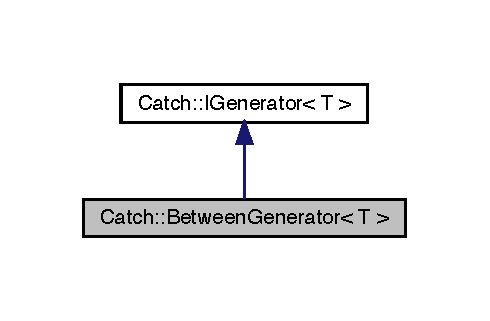
\includegraphics[width=235pt]{class_catch_1_1_between_generator__inherit__graph}
\end{center}
\end{figure}


Collaboration diagram for Catch\+:\+:Between\+Generator$<$ T $>$\+:
\nopagebreak
\begin{figure}[H]
\begin{center}
\leavevmode
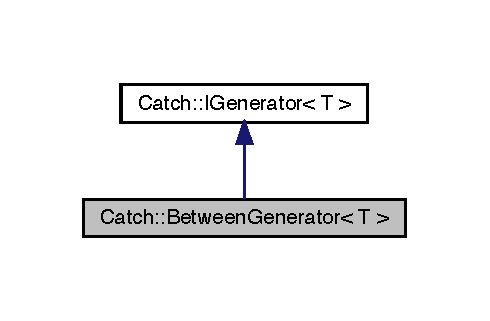
\includegraphics[width=235pt]{class_catch_1_1_between_generator__coll__graph}
\end{center}
\end{figure}
\subsection*{Public Member Functions}
\begin{DoxyCompactItemize}
\item 
\hyperlink{class_catch_1_1_between_generator_a835a057d691ae37caef660624099b51c}{Between\+Generator} (T from, T to)
\item 
virtual T \hyperlink{class_catch_1_1_between_generator_a913f74bb0c23b3bc0127abfffdabbd94}{get\+Value} (\textbf{ std\+::size\+\_\+t} index) const
\item 
virtual \textbf{ std\+::size\+\_\+t} \hyperlink{class_catch_1_1_between_generator_af65a1fe51f9b1106fc676e3dd189adb6}{size} () const
\end{DoxyCompactItemize}


\subsection{Constructor \& Destructor Documentation}
\mbox{\Hypertarget{class_catch_1_1_between_generator_a835a057d691ae37caef660624099b51c}\label{class_catch_1_1_between_generator_a835a057d691ae37caef660624099b51c}} 
\index{Catch\+::\+Between\+Generator@{Catch\+::\+Between\+Generator}!Between\+Generator@{Between\+Generator}}
\index{Between\+Generator@{Between\+Generator}!Catch\+::\+Between\+Generator@{Catch\+::\+Between\+Generator}}
\subsubsection{\texorpdfstring{Between\+Generator()}{BetweenGenerator()}}
{\footnotesize\ttfamily template$<$typename T $>$ \\
\hyperlink{class_catch_1_1_between_generator}{Catch\+::\+Between\+Generator}$<$ T $>$\+::\hyperlink{class_catch_1_1_between_generator}{Between\+Generator} (\begin{DoxyParamCaption}\item[{T}]{from,  }\item[{T}]{to }\end{DoxyParamCaption})\hspace{0.3cm}{\ttfamily [inline]}}



\subsection{Member Function Documentation}
\mbox{\Hypertarget{class_catch_1_1_between_generator_a913f74bb0c23b3bc0127abfffdabbd94}\label{class_catch_1_1_between_generator_a913f74bb0c23b3bc0127abfffdabbd94}} 
\index{Catch\+::\+Between\+Generator@{Catch\+::\+Between\+Generator}!get\+Value@{get\+Value}}
\index{get\+Value@{get\+Value}!Catch\+::\+Between\+Generator@{Catch\+::\+Between\+Generator}}
\subsubsection{\texorpdfstring{get\+Value()}{getValue()}}
{\footnotesize\ttfamily template$<$typename T $>$ \\
virtual T \hyperlink{class_catch_1_1_between_generator}{Catch\+::\+Between\+Generator}$<$ T $>$\+::get\+Value (\begin{DoxyParamCaption}\item[{\textbf{ std\+::size\+\_\+t}}]{index }\end{DoxyParamCaption}) const\hspace{0.3cm}{\ttfamily [inline]}, {\ttfamily [virtual]}}



Implements \hyperlink{struct_catch_1_1_i_generator_ad69e937cb66dba3ed9429c42abf4fce3}{Catch\+::\+I\+Generator$<$ T $>$}.

\mbox{\Hypertarget{class_catch_1_1_between_generator_af65a1fe51f9b1106fc676e3dd189adb6}\label{class_catch_1_1_between_generator_af65a1fe51f9b1106fc676e3dd189adb6}} 
\index{Catch\+::\+Between\+Generator@{Catch\+::\+Between\+Generator}!size@{size}}
\index{size@{size}!Catch\+::\+Between\+Generator@{Catch\+::\+Between\+Generator}}
\subsubsection{\texorpdfstring{size()}{size()}}
{\footnotesize\ttfamily template$<$typename T $>$ \\
virtual \textbf{ std\+::size\+\_\+t} \hyperlink{class_catch_1_1_between_generator}{Catch\+::\+Between\+Generator}$<$ T $>$\+::size (\begin{DoxyParamCaption}{ }\end{DoxyParamCaption}) const\hspace{0.3cm}{\ttfamily [inline]}, {\ttfamily [virtual]}}



Implements \hyperlink{struct_catch_1_1_i_generator_a2e317253b03e838b6065ce69719a198e}{Catch\+::\+I\+Generator$<$ T $>$}.



The documentation for this class was generated from the following file\+:\begin{DoxyCompactItemize}
\item 
src/\hyperlink{catch_8hpp}{catch.\+hpp}\end{DoxyCompactItemize}

\hypertarget{struct_b_f96}{}\section{B\+F96 Struct Reference}
\label{struct_b_f96}\index{B\+F96@{B\+F96}}
\subsection*{Public Attributes}
\begin{DoxyCompactItemize}
\item 
unsigned int \hyperlink{struct_b_f96_ac2e6f790d4f22cd59526c7286e2f9f4f}{b0}
\item 
unsigned int \hyperlink{struct_b_f96_af93c89e8a7821eb100c5efaada4f8283}{b1}
\item 
unsigned int \hyperlink{struct_b_f96_a82ff6b29a5899a12abac18f9666ed870}{b2}
\item 
int \hyperlink{struct_b_f96_a204f2f5a2bd7cd95dde8d04f777c0048}{e}
\end{DoxyCompactItemize}


\subsection{Member Data Documentation}
\mbox{\Hypertarget{struct_b_f96_ac2e6f790d4f22cd59526c7286e2f9f4f}\label{struct_b_f96_ac2e6f790d4f22cd59526c7286e2f9f4f}} 
\index{B\+F96@{B\+F96}!b0@{b0}}
\index{b0@{b0}!B\+F96@{B\+F96}}
\subsubsection{\texorpdfstring{b0}{b0}}
{\footnotesize\ttfamily unsigned int B\+F96\+::b0}

\mbox{\Hypertarget{struct_b_f96_af93c89e8a7821eb100c5efaada4f8283}\label{struct_b_f96_af93c89e8a7821eb100c5efaada4f8283}} 
\index{B\+F96@{B\+F96}!b1@{b1}}
\index{b1@{b1}!B\+F96@{B\+F96}}
\subsubsection{\texorpdfstring{b1}{b1}}
{\footnotesize\ttfamily unsigned int B\+F96\+::b1}

\mbox{\Hypertarget{struct_b_f96_a82ff6b29a5899a12abac18f9666ed870}\label{struct_b_f96_a82ff6b29a5899a12abac18f9666ed870}} 
\index{B\+F96@{B\+F96}!b2@{b2}}
\index{b2@{b2}!B\+F96@{B\+F96}}
\subsubsection{\texorpdfstring{b2}{b2}}
{\footnotesize\ttfamily unsigned int B\+F96\+::b2}

\mbox{\Hypertarget{struct_b_f96_a204f2f5a2bd7cd95dde8d04f777c0048}\label{struct_b_f96_a204f2f5a2bd7cd95dde8d04f777c0048}} 
\index{B\+F96@{B\+F96}!e@{e}}
\index{e@{e}!B\+F96@{B\+F96}}
\subsubsection{\texorpdfstring{e}{e}}
{\footnotesize\ttfamily int B\+F96\+::e}



The documentation for this struct was generated from the following file\+:\begin{DoxyCompactItemize}
\item 
src/\hyperlink{dtoa_8c}{dtoa.\+c}\end{DoxyCompactItemize}

\hypertarget{struct_bigint}{}\section{Bigint Struct Reference}
\label{struct_bigint}\index{Bigint@{Bigint}}


Collaboration diagram for Bigint\+:\nopagebreak
\begin{figure}[H]
\begin{center}
\leavevmode
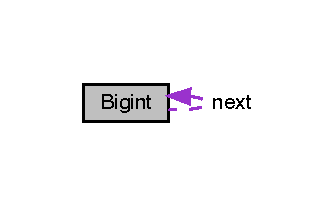
\includegraphics[width=161pt]{struct_bigint__coll__graph}
\end{center}
\end{figure}
\subsection*{Public Attributes}
\begin{DoxyCompactItemize}
\item 
struct \hyperlink{struct_bigint}{Bigint} $\ast$ \hyperlink{struct_bigint_a3a1296e26ef617e775d5e366e390e7fc}{next}
\item 
int \hyperlink{struct_bigint_a032d76e80da2f21df10c0794244d12f2}{k}
\item 
int \hyperlink{struct_bigint_a5ffcac6f95ded3bc1fc23204f46f10d0}{maxwds}
\item 
int \hyperlink{struct_bigint_a4380eb98f7653bb74d8377c0d68d6cb7}{sign}
\item 
int \hyperlink{struct_bigint_aa737992ebddb9d6a7e2d23bfecdb080e}{wds}
\item 
\hyperlink{dtoa_8c_afa5f820499f9d3fb566021c346784449}{U\+Long} \hyperlink{struct_bigint_ae56981315f471a190603887aee98ca99}{x} \mbox{[}1\mbox{]}
\end{DoxyCompactItemize}


\subsection{Member Data Documentation}
\mbox{\Hypertarget{struct_bigint_a032d76e80da2f21df10c0794244d12f2}\label{struct_bigint_a032d76e80da2f21df10c0794244d12f2}} 
\index{Bigint@{Bigint}!k@{k}}
\index{k@{k}!Bigint@{Bigint}}
\subsubsection{\texorpdfstring{k}{k}}
{\footnotesize\ttfamily int Bigint\+::k}

\mbox{\Hypertarget{struct_bigint_a5ffcac6f95ded3bc1fc23204f46f10d0}\label{struct_bigint_a5ffcac6f95ded3bc1fc23204f46f10d0}} 
\index{Bigint@{Bigint}!maxwds@{maxwds}}
\index{maxwds@{maxwds}!Bigint@{Bigint}}
\subsubsection{\texorpdfstring{maxwds}{maxwds}}
{\footnotesize\ttfamily int Bigint\+::maxwds}

\mbox{\Hypertarget{struct_bigint_a3a1296e26ef617e775d5e366e390e7fc}\label{struct_bigint_a3a1296e26ef617e775d5e366e390e7fc}} 
\index{Bigint@{Bigint}!next@{next}}
\index{next@{next}!Bigint@{Bigint}}
\subsubsection{\texorpdfstring{next}{next}}
{\footnotesize\ttfamily struct \hyperlink{struct_bigint}{Bigint}$\ast$ Bigint\+::next}

\mbox{\Hypertarget{struct_bigint_a4380eb98f7653bb74d8377c0d68d6cb7}\label{struct_bigint_a4380eb98f7653bb74d8377c0d68d6cb7}} 
\index{Bigint@{Bigint}!sign@{sign}}
\index{sign@{sign}!Bigint@{Bigint}}
\subsubsection{\texorpdfstring{sign}{sign}}
{\footnotesize\ttfamily int Bigint\+::sign}

\mbox{\Hypertarget{struct_bigint_aa737992ebddb9d6a7e2d23bfecdb080e}\label{struct_bigint_aa737992ebddb9d6a7e2d23bfecdb080e}} 
\index{Bigint@{Bigint}!wds@{wds}}
\index{wds@{wds}!Bigint@{Bigint}}
\subsubsection{\texorpdfstring{wds}{wds}}
{\footnotesize\ttfamily int Bigint\+::wds}

\mbox{\Hypertarget{struct_bigint_ae56981315f471a190603887aee98ca99}\label{struct_bigint_ae56981315f471a190603887aee98ca99}} 
\index{Bigint@{Bigint}!x@{x}}
\index{x@{x}!Bigint@{Bigint}}
\subsubsection{\texorpdfstring{x}{x}}
{\footnotesize\ttfamily \hyperlink{dtoa_8c_afa5f820499f9d3fb566021c346784449}{U\+Long} Bigint\+::x\mbox{[}1\mbox{]}}



The documentation for this struct was generated from the following file\+:\begin{DoxyCompactItemize}
\item 
src/\hyperlink{dtoa_8c}{dtoa.\+c}\end{DoxyCompactItemize}

\hypertarget{struct_binary_expression}{}\section{Binary\+Expression Struct Reference}
\label{struct_binary_expression}\index{Binary\+Expression@{Binary\+Expression}}


{\ttfamily \#include $<$ast.\+h$>$}



Collaboration diagram for Binary\+Expression\+:\nopagebreak
\begin{figure}[H]
\begin{center}
\leavevmode
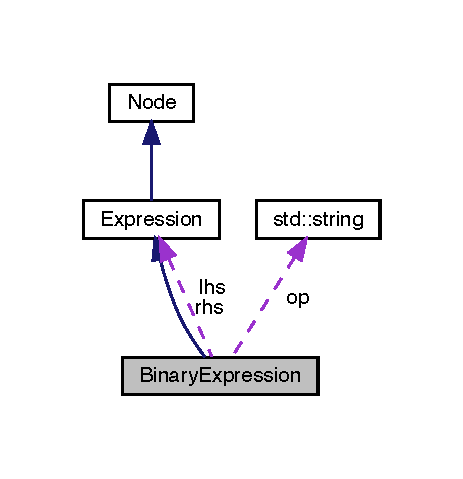
\includegraphics[width=174pt]{struct_binary_expression__coll__graph}
\end{center}
\end{figure}
\subsection*{Public Attributes}
\begin{DoxyCompactItemize}
\item 
\textbf{ std\+::string} \hyperlink{struct_binary_expression_a4c33b66e2ffc0a5ede2cdd190bf4bd75}{op}
\item 
\hyperlink{ast_8h_a4cb273a4d960cd13ea17d08f254493e8}{Expression} \hyperlink{struct_binary_expression_ab64ea2909c297e50015730abf814e82c}{lhs}
\item 
\hyperlink{ast_8h_a4cb273a4d960cd13ea17d08f254493e8}{Expression} \hyperlink{struct_binary_expression_aa25a00083ca8f135c0ffa46c527086a7}{rhs}
\end{DoxyCompactItemize}


\subsection{Member Data Documentation}
\mbox{\Hypertarget{struct_binary_expression_ab64ea2909c297e50015730abf814e82c}\label{struct_binary_expression_ab64ea2909c297e50015730abf814e82c}} 
\index{Binary\+Expression@{Binary\+Expression}!lhs@{lhs}}
\index{lhs@{lhs}!Binary\+Expression@{Binary\+Expression}}
\subsubsection{\texorpdfstring{lhs}{lhs}}
{\footnotesize\ttfamily \hyperlink{ast_8h_a4cb273a4d960cd13ea17d08f254493e8}{Expression} Binary\+Expression\+::lhs}

\mbox{\Hypertarget{struct_binary_expression_a4c33b66e2ffc0a5ede2cdd190bf4bd75}\label{struct_binary_expression_a4c33b66e2ffc0a5ede2cdd190bf4bd75}} 
\index{Binary\+Expression@{Binary\+Expression}!op@{op}}
\index{op@{op}!Binary\+Expression@{Binary\+Expression}}
\subsubsection{\texorpdfstring{op}{op}}
{\footnotesize\ttfamily \textbf{ std\+::string} Binary\+Expression\+::op}

\mbox{\Hypertarget{struct_binary_expression_aa25a00083ca8f135c0ffa46c527086a7}\label{struct_binary_expression_aa25a00083ca8f135c0ffa46c527086a7}} 
\index{Binary\+Expression@{Binary\+Expression}!rhs@{rhs}}
\index{rhs@{rhs}!Binary\+Expression@{Binary\+Expression}}
\subsubsection{\texorpdfstring{rhs}{rhs}}
{\footnotesize\ttfamily \hyperlink{ast_8h_a4cb273a4d960cd13ea17d08f254493e8}{Expression} Binary\+Expression\+::rhs}



The documentation for this struct was generated from the following file\+:\begin{DoxyCompactItemize}
\item 
src/\hyperlink{ast_8h}{ast.\+h}\end{DoxyCompactItemize}

\hypertarget{class_catch_1_1_binary_expression}{}\section{Catch\+:\+:Binary\+Expression$<$ LhsT, Op, RhsT $>$ Class Template Reference}
\label{class_catch_1_1_binary_expression}\index{Catch\+::\+Binary\+Expression$<$ Lhs\+T, Op, Rhs\+T $>$@{Catch\+::\+Binary\+Expression$<$ Lhs\+T, Op, Rhs\+T $>$}}


{\ttfamily \#include $<$catch.\+hpp$>$}



Inheritance diagram for Catch\+:\+:Binary\+Expression$<$ LhsT, Op, RhsT $>$\+:
\nopagebreak
\begin{figure}[H]
\begin{center}
\leavevmode
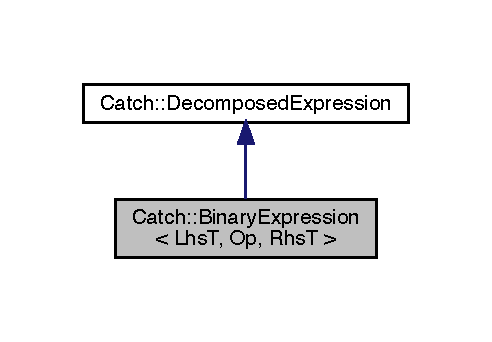
\includegraphics[width=236pt]{class_catch_1_1_binary_expression__inherit__graph}
\end{center}
\end{figure}


Collaboration diagram for Catch\+:\+:Binary\+Expression$<$ LhsT, Op, RhsT $>$\+:
\nopagebreak
\begin{figure}[H]
\begin{center}
\leavevmode
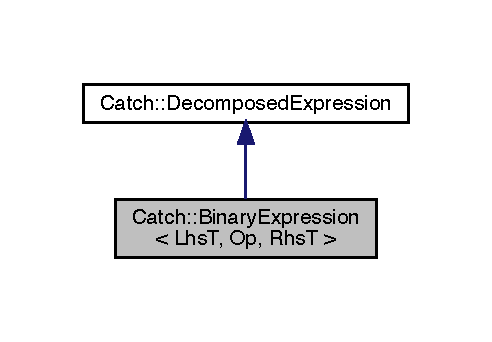
\includegraphics[width=236pt]{class_catch_1_1_binary_expression__coll__graph}
\end{center}
\end{figure}
\subsection*{Public Member Functions}
\begin{DoxyCompactItemize}
\item 
\hyperlink{class_catch_1_1_binary_expression_a0d81384761aba5f7a6d5f4fc7e7944f3}{Binary\+Expression} (\hyperlink{class_catch_1_1_result_builder}{Result\+Builder} \&rb, LhsT lhs, RhsT rhs)
\item 
\hyperlink{class_catch_1_1_binary_expression}{Binary\+Expression} \& \hyperlink{class_catch_1_1_binary_expression_a2147a858eb5866e5643d0ef321064aa1}{operator=} (\hyperlink{class_catch_1_1_binary_expression}{Binary\+Expression} \&)
\item 
void \hyperlink{class_catch_1_1_binary_expression_aa1dba7f316f70902859b8eab27692dfb}{end\+Expression} () const
\item 
virtual bool \hyperlink{class_catch_1_1_binary_expression_a4c617c0b6a73a9cafbbf900909c7c258}{is\+Binary\+Expression} () const \hyperlink{catch_8hpp_a8ecdce4d3f57835f707915ae831eb847}{C\+A\+T\+C\+H\+\_\+\+O\+V\+E\+R\+R\+I\+DE}
\item 
virtual void \hyperlink{class_catch_1_1_binary_expression_a6ed73ff9af9c229f9fa3d35d019f9e37}{reconstruct\+Expression} (\textbf{ std\+::string} \&dest) const \hyperlink{catch_8hpp_a8ecdce4d3f57835f707915ae831eb847}{C\+A\+T\+C\+H\+\_\+\+O\+V\+E\+R\+R\+I\+DE}
\end{DoxyCompactItemize}


\subsection{Constructor \& Destructor Documentation}
\mbox{\Hypertarget{class_catch_1_1_binary_expression_a0d81384761aba5f7a6d5f4fc7e7944f3}\label{class_catch_1_1_binary_expression_a0d81384761aba5f7a6d5f4fc7e7944f3}} 
\index{Catch\+::\+Binary\+Expression@{Catch\+::\+Binary\+Expression}!Binary\+Expression@{Binary\+Expression}}
\index{Binary\+Expression@{Binary\+Expression}!Catch\+::\+Binary\+Expression@{Catch\+::\+Binary\+Expression}}
\subsubsection{\texorpdfstring{Binary\+Expression()}{BinaryExpression()}}
{\footnotesize\ttfamily template$<$typename LhsT, Internal\+::\+Operator Op, typename RhsT$>$ \\
\hyperlink{class_catch_1_1_binary_expression}{Catch\+::\+Binary\+Expression}$<$ LhsT, Op, RhsT $>$\+::\hyperlink{class_catch_1_1_binary_expression}{Binary\+Expression} (\begin{DoxyParamCaption}\item[{\hyperlink{class_catch_1_1_result_builder}{Result\+Builder} \&}]{rb,  }\item[{LhsT}]{lhs,  }\item[{RhsT}]{rhs }\end{DoxyParamCaption})\hspace{0.3cm}{\ttfamily [inline]}}



\subsection{Member Function Documentation}
\mbox{\Hypertarget{class_catch_1_1_binary_expression_aa1dba7f316f70902859b8eab27692dfb}\label{class_catch_1_1_binary_expression_aa1dba7f316f70902859b8eab27692dfb}} 
\index{Catch\+::\+Binary\+Expression@{Catch\+::\+Binary\+Expression}!end\+Expression@{end\+Expression}}
\index{end\+Expression@{end\+Expression}!Catch\+::\+Binary\+Expression@{Catch\+::\+Binary\+Expression}}
\subsubsection{\texorpdfstring{end\+Expression()}{endExpression()}}
{\footnotesize\ttfamily template$<$typename LhsT, Internal\+::\+Operator Op, typename RhsT$>$ \\
void \hyperlink{class_catch_1_1_binary_expression}{Catch\+::\+Binary\+Expression}$<$ LhsT, Op, RhsT $>$\+::end\+Expression (\begin{DoxyParamCaption}{ }\end{DoxyParamCaption}) const\hspace{0.3cm}{\ttfamily [inline]}}

\mbox{\Hypertarget{class_catch_1_1_binary_expression_a4c617c0b6a73a9cafbbf900909c7c258}\label{class_catch_1_1_binary_expression_a4c617c0b6a73a9cafbbf900909c7c258}} 
\index{Catch\+::\+Binary\+Expression@{Catch\+::\+Binary\+Expression}!is\+Binary\+Expression@{is\+Binary\+Expression}}
\index{is\+Binary\+Expression@{is\+Binary\+Expression}!Catch\+::\+Binary\+Expression@{Catch\+::\+Binary\+Expression}}
\subsubsection{\texorpdfstring{is\+Binary\+Expression()}{isBinaryExpression()}}
{\footnotesize\ttfamily template$<$typename LhsT, Internal\+::\+Operator Op, typename RhsT$>$ \\
virtual bool \hyperlink{class_catch_1_1_binary_expression}{Catch\+::\+Binary\+Expression}$<$ LhsT, Op, RhsT $>$\+::is\+Binary\+Expression (\begin{DoxyParamCaption}{ }\end{DoxyParamCaption}) const\hspace{0.3cm}{\ttfamily [inline]}, {\ttfamily [virtual]}}



Reimplemented from \hyperlink{struct_catch_1_1_decomposed_expression_a1c458ece47b71f093290dbdf9bb31fdb}{Catch\+::\+Decomposed\+Expression}.

\mbox{\Hypertarget{class_catch_1_1_binary_expression_a2147a858eb5866e5643d0ef321064aa1}\label{class_catch_1_1_binary_expression_a2147a858eb5866e5643d0ef321064aa1}} 
\index{Catch\+::\+Binary\+Expression@{Catch\+::\+Binary\+Expression}!operator=@{operator=}}
\index{operator=@{operator=}!Catch\+::\+Binary\+Expression@{Catch\+::\+Binary\+Expression}}
\subsubsection{\texorpdfstring{operator=()}{operator=()}}
{\footnotesize\ttfamily template$<$typename LhsT, Internal\+::\+Operator Op, typename RhsT$>$ \\
\hyperlink{class_catch_1_1_binary_expression}{Binary\+Expression}\& \hyperlink{class_catch_1_1_binary_expression}{Catch\+::\+Binary\+Expression}$<$ LhsT, Op, RhsT $>$\+::operator= (\begin{DoxyParamCaption}\item[{\hyperlink{class_catch_1_1_binary_expression}{Binary\+Expression}$<$ LhsT, Op, RhsT $>$ \&}]{ }\end{DoxyParamCaption})}

\mbox{\Hypertarget{class_catch_1_1_binary_expression_a6ed73ff9af9c229f9fa3d35d019f9e37}\label{class_catch_1_1_binary_expression_a6ed73ff9af9c229f9fa3d35d019f9e37}} 
\index{Catch\+::\+Binary\+Expression@{Catch\+::\+Binary\+Expression}!reconstruct\+Expression@{reconstruct\+Expression}}
\index{reconstruct\+Expression@{reconstruct\+Expression}!Catch\+::\+Binary\+Expression@{Catch\+::\+Binary\+Expression}}
\subsubsection{\texorpdfstring{reconstruct\+Expression()}{reconstructExpression()}}
{\footnotesize\ttfamily template$<$typename LhsT, Internal\+::\+Operator Op, typename RhsT$>$ \\
virtual void \hyperlink{class_catch_1_1_binary_expression}{Catch\+::\+Binary\+Expression}$<$ LhsT, Op, RhsT $>$\+::reconstruct\+Expression (\begin{DoxyParamCaption}\item[{\textbf{ std\+::string} \&}]{dest }\end{DoxyParamCaption}) const\hspace{0.3cm}{\ttfamily [inline]}, {\ttfamily [virtual]}}



Implements \hyperlink{struct_catch_1_1_decomposed_expression_a9ce7f356dc96f11f80e40c82f5aa7e55}{Catch\+::\+Decomposed\+Expression}.



The documentation for this class was generated from the following file\+:\begin{DoxyCompactItemize}
\item 
src/\hyperlink{catch_8hpp}{catch.\+hpp}\end{DoxyCompactItemize}

\hypertarget{struct_binding}{}\section{Binding Struct Reference}
\label{struct_binding}\index{Binding@{Binding}}


{\ttfamily \#include $<$runtime.\+h$>$}



Collaboration diagram for Binding\+:
\nopagebreak
\begin{figure}[H]
\begin{center}
\leavevmode
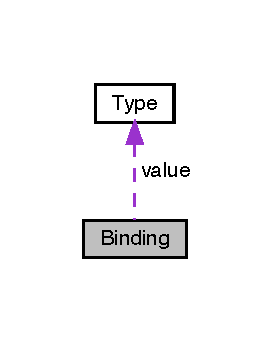
\includegraphics[width=131pt]{struct_binding__coll__graph}
\end{center}
\end{figure}
\subsection*{Public Attributes}
\begin{DoxyCompactItemize}
\item 
\hyperlink{class_type}{Type} \hyperlink{struct_binding_a71c0f96fe4d74ab7cd7e61c0609a3c4c}{value}
\item 
bool \hyperlink{struct_binding_af14c764fbd856958c8c13db394f7f30b}{is\+\_\+deletable} = true
\item 
bool \hyperlink{struct_binding_a0a6daae772f7935ec9b2ecd3d7c8b260}{is\+\_\+mutable} = true
\item 
bool \hyperlink{struct_binding_aae232d870009e0669bf9d81229eafa80}{is\+\_\+initialized} = false
\end{DoxyCompactItemize}


\subsection{Member Data Documentation}
\mbox{\Hypertarget{struct_binding_af14c764fbd856958c8c13db394f7f30b}\label{struct_binding_af14c764fbd856958c8c13db394f7f30b}} 
\index{Binding@{Binding}!is\+\_\+deletable@{is\+\_\+deletable}}
\index{is\+\_\+deletable@{is\+\_\+deletable}!Binding@{Binding}}
\subsubsection{\texorpdfstring{is\+\_\+deletable}{is\_deletable}}
{\footnotesize\ttfamily bool Binding\+::is\+\_\+deletable = true}

\mbox{\Hypertarget{struct_binding_aae232d870009e0669bf9d81229eafa80}\label{struct_binding_aae232d870009e0669bf9d81229eafa80}} 
\index{Binding@{Binding}!is\+\_\+initialized@{is\+\_\+initialized}}
\index{is\+\_\+initialized@{is\+\_\+initialized}!Binding@{Binding}}
\subsubsection{\texorpdfstring{is\+\_\+initialized}{is\_initialized}}
{\footnotesize\ttfamily bool Binding\+::is\+\_\+initialized = false}

\mbox{\Hypertarget{struct_binding_a0a6daae772f7935ec9b2ecd3d7c8b260}\label{struct_binding_a0a6daae772f7935ec9b2ecd3d7c8b260}} 
\index{Binding@{Binding}!is\+\_\+mutable@{is\+\_\+mutable}}
\index{is\+\_\+mutable@{is\+\_\+mutable}!Binding@{Binding}}
\subsubsection{\texorpdfstring{is\+\_\+mutable}{is\_mutable}}
{\footnotesize\ttfamily bool Binding\+::is\+\_\+mutable = true}

\mbox{\Hypertarget{struct_binding_a71c0f96fe4d74ab7cd7e61c0609a3c4c}\label{struct_binding_a71c0f96fe4d74ab7cd7e61c0609a3c4c}} 
\index{Binding@{Binding}!value@{value}}
\index{value@{value}!Binding@{Binding}}
\subsubsection{\texorpdfstring{value}{value}}
{\footnotesize\ttfamily \hyperlink{class_type}{Type} Binding\+::value}



The documentation for this struct was generated from the following file\+:\begin{DoxyCompactItemize}
\item 
src/\hyperlink{runtime_8h}{runtime.\+h}\end{DoxyCompactItemize}

\hypertarget{struct_block}{}\section{Block Struct Reference}
\label{struct_block}\index{Block@{Block}}


{\ttfamily \#include $<$ast.\+h$>$}



Inheritance diagram for Block\+:\nopagebreak
\begin{figure}[H]
\begin{center}
\leavevmode
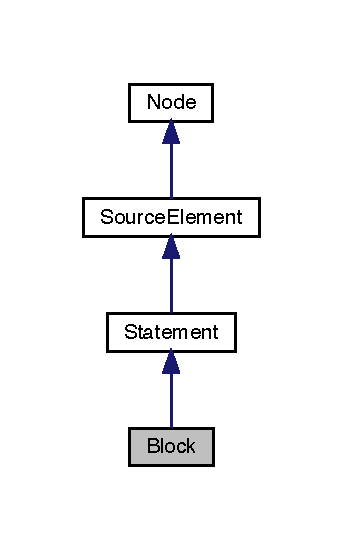
\includegraphics[width=164pt]{struct_block__inherit__graph}
\end{center}
\end{figure}


Collaboration diagram for Block\+:\nopagebreak
\begin{figure}[H]
\begin{center}
\leavevmode
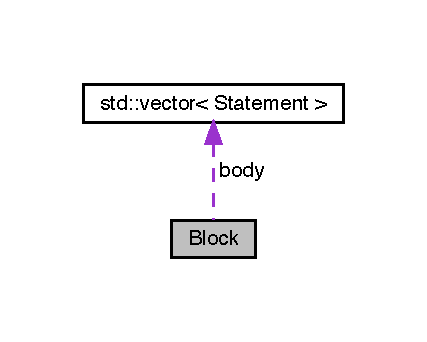
\includegraphics[width=294pt]{struct_block__coll__graph}
\end{center}
\end{figure}
\subsection*{Public Member Functions}
\begin{DoxyCompactItemize}
\item 
\hyperlink{struct_block_a757d46b60b5babb84c5c466b99679c2d}{Block} (\hyperlink{struct_statement_list}{Statement\+List} $\ast$\hyperlink{struct_block_a05207097167e9263252079d78f3d9358}{body}=nullptr)
\item 
void \hyperlink{struct_block_ac00e5c0ee8486dbdc7cb91dd5a6b34e1}{accept} (\hyperlink{struct_visitor}{Visitor} \&visitor) const override
\item 
const char $\ast$ \hyperlink{struct_block_a0a495712f07ce103494469c87a8352c2}{type} () const override
\end{DoxyCompactItemize}
\subsection*{Public Attributes}
\begin{DoxyCompactItemize}
\item 
\hyperlink{struct_statement_list}{Statement\+List} $\ast$ \hyperlink{struct_block_a05207097167e9263252079d78f3d9358}{body}
\end{DoxyCompactItemize}


\subsection{Constructor \& Destructor Documentation}
\mbox{\Hypertarget{struct_block_a757d46b60b5babb84c5c466b99679c2d}\label{struct_block_a757d46b60b5babb84c5c466b99679c2d}} 
\index{Block@{Block}!Block@{Block}}
\index{Block@{Block}!Block@{Block}}
\subsubsection{\texorpdfstring{Block()}{Block()}}
{\footnotesize\ttfamily Block\+::\+Block (\begin{DoxyParamCaption}\item[{\hyperlink{struct_statement_list}{Statement\+List} $\ast$}]{body = {\ttfamily nullptr} }\end{DoxyParamCaption})\hspace{0.3cm}{\ttfamily [inline]}}



\subsection{Member Function Documentation}
\mbox{\Hypertarget{struct_block_ac00e5c0ee8486dbdc7cb91dd5a6b34e1}\label{struct_block_ac00e5c0ee8486dbdc7cb91dd5a6b34e1}} 
\index{Block@{Block}!accept@{accept}}
\index{accept@{accept}!Block@{Block}}
\subsubsection{\texorpdfstring{accept()}{accept()}}
{\footnotesize\ttfamily void Block\+::accept (\begin{DoxyParamCaption}\item[{\hyperlink{struct_visitor}{Visitor} \&}]{visitor }\end{DoxyParamCaption}) const\hspace{0.3cm}{\ttfamily [inline]}, {\ttfamily [override]}, {\ttfamily [virtual]}}



Implements \hyperlink{struct_node_a10bd7af968140bbf5fa461298a969c71}{Node}.

\mbox{\Hypertarget{struct_block_a0a495712f07ce103494469c87a8352c2}\label{struct_block_a0a495712f07ce103494469c87a8352c2}} 
\index{Block@{Block}!type@{type}}
\index{type@{type}!Block@{Block}}
\subsubsection{\texorpdfstring{type()}{type()}}
{\footnotesize\ttfamily const char$\ast$ Block\+::type (\begin{DoxyParamCaption}{ }\end{DoxyParamCaption}) const\hspace{0.3cm}{\ttfamily [inline]}, {\ttfamily [override]}, {\ttfamily [virtual]}}



Implements \hyperlink{struct_node_a82f29420d0a38efcc370352528e94e9b}{Node}.



\subsection{Member Data Documentation}
\mbox{\Hypertarget{struct_block_a05207097167e9263252079d78f3d9358}\label{struct_block_a05207097167e9263252079d78f3d9358}} 
\index{Block@{Block}!body@{body}}
\index{body@{body}!Block@{Block}}
\subsubsection{\texorpdfstring{body}{body}}
{\footnotesize\ttfamily \hyperlink{struct_statement_list}{Statement\+List}$\ast$ Block\+::body}



The documentation for this struct was generated from the following file\+:\begin{DoxyCompactItemize}
\item 
src/\hyperlink{ast_8h}{ast.\+h}\end{DoxyCompactItemize}

\hypertarget{struct_boolean}{}\section{Boolean Struct Reference}
\label{struct_boolean}\index{Boolean@{Boolean}}


{\ttfamily \#include $<$value.\+h$>$}

\subsection*{Public Attributes}
\begin{DoxyCompactItemize}
\item 
bool \hyperlink{struct_boolean_a8e44c7f95d984f2dc8c6974f607b2b36}{value}
\end{DoxyCompactItemize}


\subsection{Member Data Documentation}
\mbox{\Hypertarget{struct_boolean_a8e44c7f95d984f2dc8c6974f607b2b36}\label{struct_boolean_a8e44c7f95d984f2dc8c6974f607b2b36}} 
\index{Boolean@{Boolean}!value@{value}}
\index{value@{value}!Boolean@{Boolean}}
\subsubsection{\texorpdfstring{value}{value}}
{\footnotesize\ttfamily bool Boolean\+::value}



The documentation for this struct was generated from the following file\+:\begin{DoxyCompactItemize}
\item 
src/\hyperlink{value_8h}{value.\+h}\end{DoxyCompactItemize}

\hypertarget{struct_boolean_literal}{}\section{Boolean\+Literal Struct Reference}
\label{struct_boolean_literal}\index{Boolean\+Literal@{Boolean\+Literal}}


{\ttfamily \#include $<$ast.\+h$>$}



Inheritance diagram for Boolean\+Literal\+:\nopagebreak
\begin{figure}[H]
\begin{center}
\leavevmode
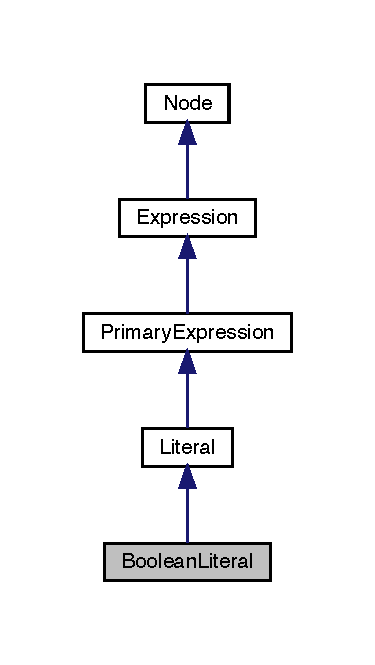
\includegraphics[width=160pt]{struct_boolean_literal__inherit__graph}
\end{center}
\end{figure}


Collaboration diagram for Boolean\+Literal\+:
\nopagebreak
\begin{figure}[H]
\begin{center}
\leavevmode
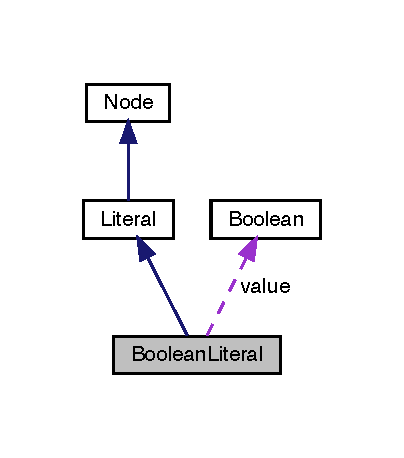
\includegraphics[width=194pt]{struct_boolean_literal__coll__graph}
\end{center}
\end{figure}
\subsection*{Public Member Functions}
\begin{DoxyCompactItemize}
\item 
\hyperlink{struct_boolean_literal_a62943a1e1523297b1ea0372d1a5fbbfb}{Boolean\+Literal} (\hyperlink{struct_boolean}{Boolean} \hyperlink{struct_boolean_literal_af74f8eba8c2ea30656de4c4919f5778d}{value})
\item 
void \hyperlink{struct_boolean_literal_aeb7a30e2b22ac6ad12723da1e72087c5}{accept} (\hyperlink{struct_visitor}{Visitor} \&visitor) const override
\item 
const char $\ast$ \hyperlink{struct_boolean_literal_aa10a3ecbeefe15607c3ac43ed63ba8da}{type} () const override
\end{DoxyCompactItemize}
\subsection*{Public Attributes}
\begin{DoxyCompactItemize}
\item 
\hyperlink{struct_boolean}{Boolean} \hyperlink{struct_boolean_literal_af74f8eba8c2ea30656de4c4919f5778d}{value}
\end{DoxyCompactItemize}


\subsection{Constructor \& Destructor Documentation}
\mbox{\Hypertarget{struct_boolean_literal_a62943a1e1523297b1ea0372d1a5fbbfb}\label{struct_boolean_literal_a62943a1e1523297b1ea0372d1a5fbbfb}} 
\index{Boolean\+Literal@{Boolean\+Literal}!Boolean\+Literal@{Boolean\+Literal}}
\index{Boolean\+Literal@{Boolean\+Literal}!Boolean\+Literal@{Boolean\+Literal}}
\subsubsection{\texorpdfstring{Boolean\+Literal()}{BooleanLiteral()}}
{\footnotesize\ttfamily Boolean\+Literal\+::\+Boolean\+Literal (\begin{DoxyParamCaption}\item[{\hyperlink{struct_boolean}{Boolean}}]{value }\end{DoxyParamCaption})\hspace{0.3cm}{\ttfamily [inline]}}



\subsection{Member Function Documentation}
\mbox{\Hypertarget{struct_boolean_literal_aeb7a30e2b22ac6ad12723da1e72087c5}\label{struct_boolean_literal_aeb7a30e2b22ac6ad12723da1e72087c5}} 
\index{Boolean\+Literal@{Boolean\+Literal}!accept@{accept}}
\index{accept@{accept}!Boolean\+Literal@{Boolean\+Literal}}
\subsubsection{\texorpdfstring{accept()}{accept()}}
{\footnotesize\ttfamily void Boolean\+Literal\+::accept (\begin{DoxyParamCaption}\item[{\hyperlink{struct_visitor}{Visitor} \&}]{visitor }\end{DoxyParamCaption}) const\hspace{0.3cm}{\ttfamily [inline]}, {\ttfamily [override]}, {\ttfamily [virtual]}}



Implements \hyperlink{struct_node_a10bd7af968140bbf5fa461298a969c71}{Node}.

\mbox{\Hypertarget{struct_boolean_literal_aa10a3ecbeefe15607c3ac43ed63ba8da}\label{struct_boolean_literal_aa10a3ecbeefe15607c3ac43ed63ba8da}} 
\index{Boolean\+Literal@{Boolean\+Literal}!type@{type}}
\index{type@{type}!Boolean\+Literal@{Boolean\+Literal}}
\subsubsection{\texorpdfstring{type()}{type()}}
{\footnotesize\ttfamily const char$\ast$ Boolean\+Literal\+::type (\begin{DoxyParamCaption}{ }\end{DoxyParamCaption}) const\hspace{0.3cm}{\ttfamily [inline]}, {\ttfamily [override]}, {\ttfamily [virtual]}}



Implements \hyperlink{struct_node_a82f29420d0a38efcc370352528e94e9b}{Node}.



\subsection{Member Data Documentation}
\mbox{\Hypertarget{struct_boolean_literal_af74f8eba8c2ea30656de4c4919f5778d}\label{struct_boolean_literal_af74f8eba8c2ea30656de4c4919f5778d}} 
\index{Boolean\+Literal@{Boolean\+Literal}!value@{value}}
\index{value@{value}!Boolean\+Literal@{Boolean\+Literal}}
\subsubsection{\texorpdfstring{value}{value}}
{\footnotesize\ttfamily \hyperlink{struct_boolean}{Boolean} Boolean\+Literal\+::value}



The documentation for this struct was generated from the following file\+:\begin{DoxyCompactItemize}
\item 
src/\hyperlink{ast_8h}{ast.\+h}\end{DoxyCompactItemize}

\hypertarget{struct_catch_1_1_detail_1_1_borg_type}{}\section{Catch\+:\+:Detail\+:\+:Borg\+Type Struct Reference}
\label{struct_catch_1_1_detail_1_1_borg_type}\index{Catch\+::\+Detail\+::\+Borg\+Type@{Catch\+::\+Detail\+::\+Borg\+Type}}


{\ttfamily \#include $<$catch.\+hpp$>$}

\subsection*{Public Member Functions}
\begin{DoxyCompactItemize}
\item 
{\footnotesize template$<$typename T $>$ }\\\hyperlink{struct_catch_1_1_detail_1_1_borg_type_a780a9946ed0d654f0bfc043c8fc505d8}{Borg\+Type} (T const \&)
\end{DoxyCompactItemize}


\subsection{Constructor \& Destructor Documentation}
\mbox{\Hypertarget{struct_catch_1_1_detail_1_1_borg_type_a780a9946ed0d654f0bfc043c8fc505d8}\label{struct_catch_1_1_detail_1_1_borg_type_a780a9946ed0d654f0bfc043c8fc505d8}} 
\index{Catch\+::\+Detail\+::\+Borg\+Type@{Catch\+::\+Detail\+::\+Borg\+Type}!Borg\+Type@{Borg\+Type}}
\index{Borg\+Type@{Borg\+Type}!Catch\+::\+Detail\+::\+Borg\+Type@{Catch\+::\+Detail\+::\+Borg\+Type}}
\subsubsection{\texorpdfstring{Borg\+Type()}{BorgType()}}
{\footnotesize\ttfamily template$<$typename T $>$ \\
Catch\+::\+Detail\+::\+Borg\+Type\+::\+Borg\+Type (\begin{DoxyParamCaption}\item[{T const \&}]{ }\end{DoxyParamCaption})}



The documentation for this struct was generated from the following file\+:\begin{DoxyCompactItemize}
\item 
src/\hyperlink{catch_8hpp}{catch.\+hpp}\end{DoxyCompactItemize}

\hypertarget{struct_break_statement}{}\section{Break\+Statement Struct Reference}
\label{struct_break_statement}\index{Break\+Statement@{Break\+Statement}}


{\ttfamily \#include $<$ast.\+h$>$}

\subsection*{Public Attributes}
\begin{DoxyCompactItemize}
\item 
boost\+::optional$<$ \hyperlink{struct_identifier}{Identifier} $>$ \hyperlink{struct_break_statement_a0367fe642b46069be309b05e05b547c5}{label}
\end{DoxyCompactItemize}


\subsection{Member Data Documentation}
\mbox{\Hypertarget{struct_break_statement_a0367fe642b46069be309b05e05b547c5}\label{struct_break_statement_a0367fe642b46069be309b05e05b547c5}} 
\index{Break\+Statement@{Break\+Statement}!label@{label}}
\index{label@{label}!Break\+Statement@{Break\+Statement}}
\subsubsection{\texorpdfstring{label}{label}}
{\footnotesize\ttfamily boost\+::optional$<$\hyperlink{struct_identifier}{Identifier}$>$ Break\+Statement\+::label}



The documentation for this struct was generated from the following file\+:\begin{DoxyCompactItemize}
\item 
src/\hyperlink{ast_8h}{ast.\+h}\end{DoxyCompactItemize}

\hypertarget{struct_call_expression}{}\section{Call\+Expression Struct Reference}
\label{struct_call_expression}\index{Call\+Expression@{Call\+Expression}}


{\ttfamily \#include $<$ast.\+h$>$}



Inheritance diagram for Call\+Expression\+:
\nopagebreak
\begin{figure}[H]
\begin{center}
\leavevmode
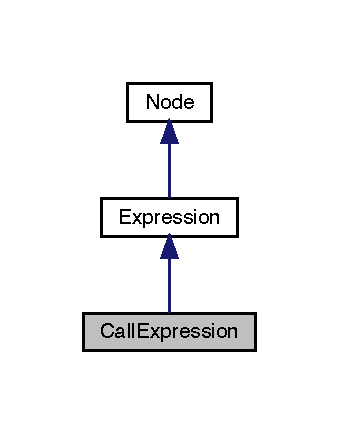
\includegraphics[width=163pt]{struct_call_expression__inherit__graph}
\end{center}
\end{figure}


Collaboration diagram for Call\+Expression\+:
\nopagebreak
\begin{figure}[H]
\begin{center}
\leavevmode
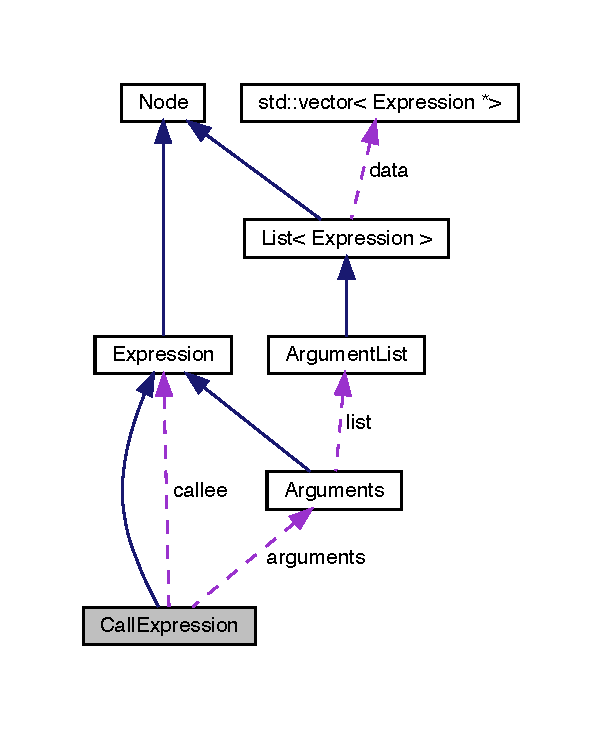
\includegraphics[width=289pt]{struct_call_expression__coll__graph}
\end{center}
\end{figure}
\subsection*{Public Member Functions}
\begin{DoxyCompactItemize}
\item 
\hyperlink{struct_call_expression_a7e6da0437a5f82430af5f31779b830d7}{Call\+Expression} (\hyperlink{struct_expression}{Expression} $\ast$\hyperlink{struct_call_expression_a2d77ccd1a2d6f34d718063f0eb47bc21}{callee}, \hyperlink{struct_arguments}{Arguments} $\ast$\hyperlink{struct_call_expression_ad2dad57df529ef1ef06b43cd438598bd}{arguments}=nullptr)
\item 
void \hyperlink{struct_call_expression_a5be626b61944a97f2a6015b632432513}{accept} (\hyperlink{struct_visitor}{Visitor} \&visitor) const override
\item 
const char $\ast$ \hyperlink{struct_call_expression_ae2891106618133745e00ac92a6b6b4fd}{type} () const override
\end{DoxyCompactItemize}
\subsection*{Public Attributes}
\begin{DoxyCompactItemize}
\item 
\hyperlink{struct_expression}{Expression} $\ast$ \hyperlink{struct_call_expression_a2d77ccd1a2d6f34d718063f0eb47bc21}{callee}
\item 
\hyperlink{struct_arguments}{Arguments} $\ast$ \hyperlink{struct_call_expression_ad2dad57df529ef1ef06b43cd438598bd}{arguments}
\end{DoxyCompactItemize}


\subsection{Constructor \& Destructor Documentation}
\mbox{\Hypertarget{struct_call_expression_a7e6da0437a5f82430af5f31779b830d7}\label{struct_call_expression_a7e6da0437a5f82430af5f31779b830d7}} 
\index{Call\+Expression@{Call\+Expression}!Call\+Expression@{Call\+Expression}}
\index{Call\+Expression@{Call\+Expression}!Call\+Expression@{Call\+Expression}}
\subsubsection{\texorpdfstring{Call\+Expression()}{CallExpression()}}
{\footnotesize\ttfamily Call\+Expression\+::\+Call\+Expression (\begin{DoxyParamCaption}\item[{\hyperlink{struct_expression}{Expression} $\ast$}]{callee,  }\item[{\hyperlink{struct_arguments}{Arguments} $\ast$}]{arguments = {\ttfamily nullptr} }\end{DoxyParamCaption})\hspace{0.3cm}{\ttfamily [inline]}}



\subsection{Member Function Documentation}
\mbox{\Hypertarget{struct_call_expression_a5be626b61944a97f2a6015b632432513}\label{struct_call_expression_a5be626b61944a97f2a6015b632432513}} 
\index{Call\+Expression@{Call\+Expression}!accept@{accept}}
\index{accept@{accept}!Call\+Expression@{Call\+Expression}}
\subsubsection{\texorpdfstring{accept()}{accept()}}
{\footnotesize\ttfamily void Call\+Expression\+::accept (\begin{DoxyParamCaption}\item[{\hyperlink{struct_visitor}{Visitor} \&}]{visitor }\end{DoxyParamCaption}) const\hspace{0.3cm}{\ttfamily [inline]}, {\ttfamily [override]}, {\ttfamily [virtual]}}



Implements \hyperlink{struct_node_a10bd7af968140bbf5fa461298a969c71}{Node}.

\mbox{\Hypertarget{struct_call_expression_ae2891106618133745e00ac92a6b6b4fd}\label{struct_call_expression_ae2891106618133745e00ac92a6b6b4fd}} 
\index{Call\+Expression@{Call\+Expression}!type@{type}}
\index{type@{type}!Call\+Expression@{Call\+Expression}}
\subsubsection{\texorpdfstring{type()}{type()}}
{\footnotesize\ttfamily const char$\ast$ Call\+Expression\+::type (\begin{DoxyParamCaption}{ }\end{DoxyParamCaption}) const\hspace{0.3cm}{\ttfamily [inline]}, {\ttfamily [override]}, {\ttfamily [virtual]}}



Implements \hyperlink{struct_node_a82f29420d0a38efcc370352528e94e9b}{Node}.



\subsection{Member Data Documentation}
\mbox{\Hypertarget{struct_call_expression_ad2dad57df529ef1ef06b43cd438598bd}\label{struct_call_expression_ad2dad57df529ef1ef06b43cd438598bd}} 
\index{Call\+Expression@{Call\+Expression}!arguments@{arguments}}
\index{arguments@{arguments}!Call\+Expression@{Call\+Expression}}
\subsubsection{\texorpdfstring{arguments}{arguments}}
{\footnotesize\ttfamily \hyperlink{struct_arguments}{Arguments}$\ast$ Call\+Expression\+::arguments}

\mbox{\Hypertarget{struct_call_expression_a2d77ccd1a2d6f34d718063f0eb47bc21}\label{struct_call_expression_a2d77ccd1a2d6f34d718063f0eb47bc21}} 
\index{Call\+Expression@{Call\+Expression}!callee@{callee}}
\index{callee@{callee}!Call\+Expression@{Call\+Expression}}
\subsubsection{\texorpdfstring{callee}{callee}}
{\footnotesize\ttfamily \hyperlink{struct_expression}{Expression}$\ast$ Call\+Expression\+::callee}



The documentation for this struct was generated from the following file\+:\begin{DoxyCompactItemize}
\item 
src/\hyperlink{ast_8h}{ast.\+h}\end{DoxyCompactItemize}

\hypertarget{struct_case_block}{}\section{Case\+Block Struct Reference}
\label{struct_case_block}\index{Case\+Block@{Case\+Block}}


{\ttfamily \#include $<$ast.\+h$>$}



Inheritance diagram for Case\+Block\+:\nopagebreak
\begin{figure}[H]
\begin{center}
\leavevmode
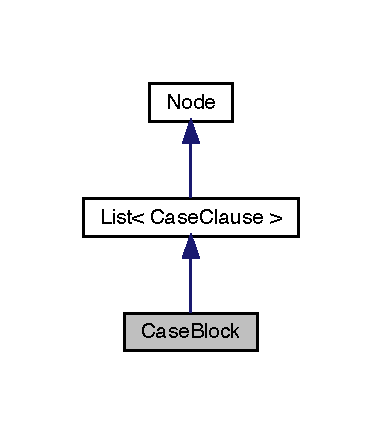
\includegraphics[width=183pt]{struct_case_block__inherit__graph}
\end{center}
\end{figure}


Collaboration diagram for Case\+Block\+:\nopagebreak
\begin{figure}[H]
\begin{center}
\leavevmode
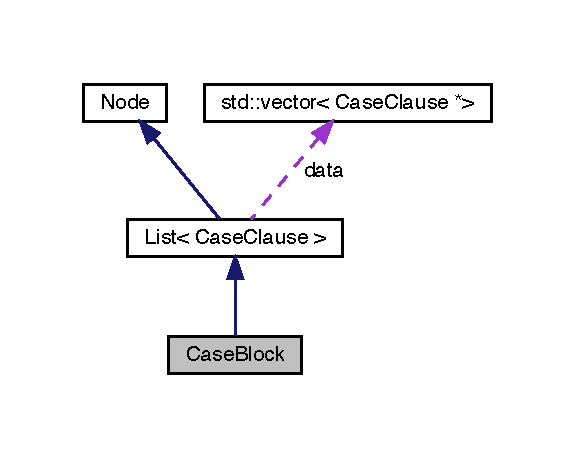
\includegraphics[width=276pt]{struct_case_block__coll__graph}
\end{center}
\end{figure}
\subsection*{Additional Inherited Members}


The documentation for this struct was generated from the following file\+:\begin{DoxyCompactItemize}
\item 
src/\hyperlink{ast_8h}{ast.\+h}\end{DoxyCompactItemize}

\hypertarget{struct_case_clause}{}\section{Case\+Clause Struct Reference}
\label{struct_case_clause}\index{Case\+Clause@{Case\+Clause}}


{\ttfamily \#include $<$ast.\+h$>$}



Inheritance diagram for Case\+Clause\+:\nopagebreak
\begin{figure}[H]
\begin{center}
\leavevmode
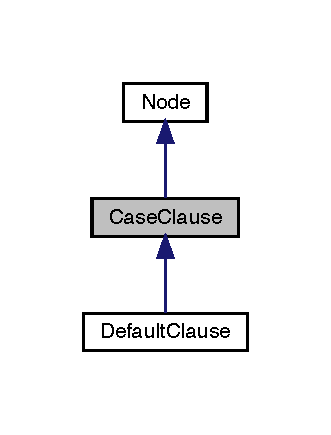
\includegraphics[width=159pt]{struct_case_clause__inherit__graph}
\end{center}
\end{figure}


Collaboration diagram for Case\+Clause\+:\nopagebreak
\begin{figure}[H]
\begin{center}
\leavevmode
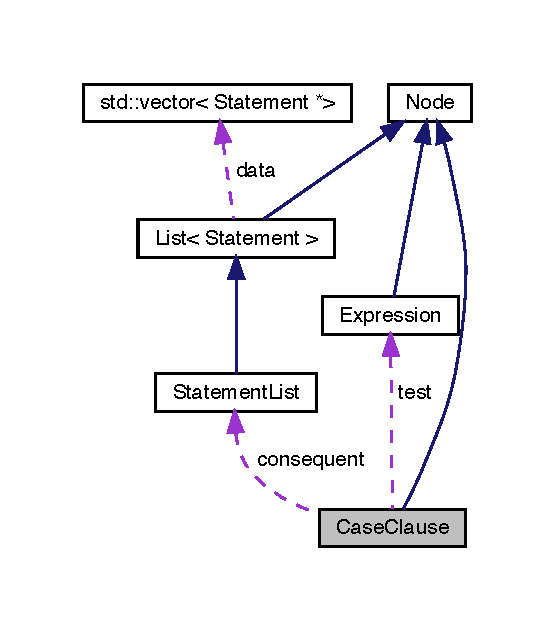
\includegraphics[width=266pt]{struct_case_clause__coll__graph}
\end{center}
\end{figure}
\subsection*{Public Member Functions}
\begin{DoxyCompactItemize}
\item 
\hyperlink{struct_case_clause_a05d8bf165e3a4796247b5fbf1f71d3e5}{Case\+Clause} (\hyperlink{struct_expression}{Expression} $\ast$\hyperlink{struct_case_clause_a80b6f256f3d9910250e4b8433ea75d7f}{test}, \hyperlink{struct_statement_list}{Statement\+List} $\ast$\hyperlink{struct_case_clause_a3e6914411610d1893b61172521e11288}{consequent})
\item 
void \hyperlink{struct_case_clause_a5bbee9ea9ca206c09b8b79f8c96720a1}{accept} (\hyperlink{struct_visitor}{Visitor} \&visitor) const override
\item 
const char $\ast$ \hyperlink{struct_case_clause_a9dcb0a1a072df7d577b272c6bbb3c6dc}{type} () const override
\item 
bool \hyperlink{struct_case_clause_a8ef15339531ef33d3ae335d96317b30a}{is\+\_\+default} () const
\end{DoxyCompactItemize}
\subsection*{Public Attributes}
\begin{DoxyCompactItemize}
\item 
\hyperlink{struct_expression}{Expression} $\ast$ \hyperlink{struct_case_clause_a80b6f256f3d9910250e4b8433ea75d7f}{test} = nullptr
\item 
\hyperlink{struct_statement_list}{Statement\+List} $\ast$ \hyperlink{struct_case_clause_a3e6914411610d1893b61172521e11288}{consequent}
\end{DoxyCompactItemize}


\subsection{Constructor \& Destructor Documentation}
\mbox{\Hypertarget{struct_case_clause_a05d8bf165e3a4796247b5fbf1f71d3e5}\label{struct_case_clause_a05d8bf165e3a4796247b5fbf1f71d3e5}} 
\index{Case\+Clause@{Case\+Clause}!Case\+Clause@{Case\+Clause}}
\index{Case\+Clause@{Case\+Clause}!Case\+Clause@{Case\+Clause}}
\subsubsection{\texorpdfstring{Case\+Clause()}{CaseClause()}}
{\footnotesize\ttfamily Case\+Clause\+::\+Case\+Clause (\begin{DoxyParamCaption}\item[{\hyperlink{struct_expression}{Expression} $\ast$}]{test,  }\item[{\hyperlink{struct_statement_list}{Statement\+List} $\ast$}]{consequent }\end{DoxyParamCaption})\hspace{0.3cm}{\ttfamily [inline]}}



\subsection{Member Function Documentation}
\mbox{\Hypertarget{struct_case_clause_a5bbee9ea9ca206c09b8b79f8c96720a1}\label{struct_case_clause_a5bbee9ea9ca206c09b8b79f8c96720a1}} 
\index{Case\+Clause@{Case\+Clause}!accept@{accept}}
\index{accept@{accept}!Case\+Clause@{Case\+Clause}}
\subsubsection{\texorpdfstring{accept()}{accept()}}
{\footnotesize\ttfamily void Case\+Clause\+::accept (\begin{DoxyParamCaption}\item[{\hyperlink{struct_visitor}{Visitor} \&}]{visitor }\end{DoxyParamCaption}) const\hspace{0.3cm}{\ttfamily [inline]}, {\ttfamily [override]}, {\ttfamily [virtual]}}



Implements \hyperlink{struct_node_a10bd7af968140bbf5fa461298a969c71}{Node}.



Reimplemented in \hyperlink{struct_default_clause_ade62e79cf9ad891d974528e1e172e2b6}{Default\+Clause}.

\mbox{\Hypertarget{struct_case_clause_a8ef15339531ef33d3ae335d96317b30a}\label{struct_case_clause_a8ef15339531ef33d3ae335d96317b30a}} 
\index{Case\+Clause@{Case\+Clause}!is\+\_\+default@{is\+\_\+default}}
\index{is\+\_\+default@{is\+\_\+default}!Case\+Clause@{Case\+Clause}}
\subsubsection{\texorpdfstring{is\+\_\+default()}{is\_default()}}
{\footnotesize\ttfamily bool Case\+Clause\+::is\+\_\+default (\begin{DoxyParamCaption}{ }\end{DoxyParamCaption}) const\hspace{0.3cm}{\ttfamily [inline]}}

\mbox{\Hypertarget{struct_case_clause_a9dcb0a1a072df7d577b272c6bbb3c6dc}\label{struct_case_clause_a9dcb0a1a072df7d577b272c6bbb3c6dc}} 
\index{Case\+Clause@{Case\+Clause}!type@{type}}
\index{type@{type}!Case\+Clause@{Case\+Clause}}
\subsubsection{\texorpdfstring{type()}{type()}}
{\footnotesize\ttfamily const char$\ast$ Case\+Clause\+::type (\begin{DoxyParamCaption}{ }\end{DoxyParamCaption}) const\hspace{0.3cm}{\ttfamily [inline]}, {\ttfamily [override]}, {\ttfamily [virtual]}}



Implements \hyperlink{struct_node_a82f29420d0a38efcc370352528e94e9b}{Node}.



Reimplemented in \hyperlink{struct_default_clause_a464358dcd7e4e13287482d3c858f3538}{Default\+Clause}.



\subsection{Member Data Documentation}
\mbox{\Hypertarget{struct_case_clause_a3e6914411610d1893b61172521e11288}\label{struct_case_clause_a3e6914411610d1893b61172521e11288}} 
\index{Case\+Clause@{Case\+Clause}!consequent@{consequent}}
\index{consequent@{consequent}!Case\+Clause@{Case\+Clause}}
\subsubsection{\texorpdfstring{consequent}{consequent}}
{\footnotesize\ttfamily \hyperlink{struct_statement_list}{Statement\+List}$\ast$ Case\+Clause\+::consequent}

\mbox{\Hypertarget{struct_case_clause_a80b6f256f3d9910250e4b8433ea75d7f}\label{struct_case_clause_a80b6f256f3d9910250e4b8433ea75d7f}} 
\index{Case\+Clause@{Case\+Clause}!test@{test}}
\index{test@{test}!Case\+Clause@{Case\+Clause}}
\subsubsection{\texorpdfstring{test}{test}}
{\footnotesize\ttfamily \hyperlink{struct_expression}{Expression}$\ast$ Case\+Clause\+::test = nullptr}



The documentation for this struct was generated from the following file\+:\begin{DoxyCompactItemize}
\item 
src/\hyperlink{ast_8h}{ast.\+h}\end{DoxyCompactItemize}

\hypertarget{struct_catch_1_1_matchers_1_1_std_string_1_1_cased_string}{}\section{Catch\+:\+:Matchers\+:\+:Std\+String\+:\+:Cased\+String Struct Reference}
\label{struct_catch_1_1_matchers_1_1_std_string_1_1_cased_string}\index{Catch\+::\+Matchers\+::\+Std\+String\+::\+Cased\+String@{Catch\+::\+Matchers\+::\+Std\+String\+::\+Cased\+String}}


{\ttfamily \#include $<$catch.\+hpp$>$}



Collaboration diagram for Catch\+:\+:Matchers\+:\+:Std\+String\+:\+:Cased\+String\+:
\nopagebreak
\begin{figure}[H]
\begin{center}
\leavevmode
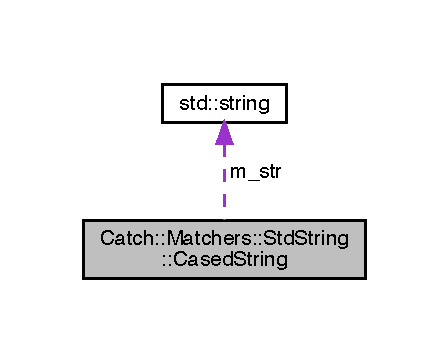
\includegraphics[width=215pt]{struct_catch_1_1_matchers_1_1_std_string_1_1_cased_string__coll__graph}
\end{center}
\end{figure}
\subsection*{Public Member Functions}
\begin{DoxyCompactItemize}
\item 
\hyperlink{struct_catch_1_1_matchers_1_1_std_string_1_1_cased_string_aa88bbc5acd2bff22351d8d4b1816b561}{Cased\+String} (\textbf{ std\+::string} const \&str, \hyperlink{struct_catch_1_1_case_sensitive_aad49d3aee2d97066642fffa919685c6a}{Case\+Sensitive\+::\+Choice} case\+Sensitivity)
\item 
\textbf{ std\+::string} \hyperlink{struct_catch_1_1_matchers_1_1_std_string_1_1_cased_string_a77639b1165c01f424ee0e96f53335010}{adjust\+String} (\textbf{ std\+::string} const \&str) const
\item 
\textbf{ std\+::string} \hyperlink{struct_catch_1_1_matchers_1_1_std_string_1_1_cased_string_a9759155344d696b2476d764a1d95fcc9}{case\+Sensitivity\+Suffix} () const
\end{DoxyCompactItemize}
\subsection*{Public Attributes}
\begin{DoxyCompactItemize}
\item 
\hyperlink{struct_catch_1_1_case_sensitive_aad49d3aee2d97066642fffa919685c6a}{Case\+Sensitive\+::\+Choice} \hyperlink{struct_catch_1_1_matchers_1_1_std_string_1_1_cased_string_ae1c2864c986941536a6e94cca0528f92}{m\+\_\+case\+Sensitivity}
\item 
\textbf{ std\+::string} \hyperlink{struct_catch_1_1_matchers_1_1_std_string_1_1_cased_string_ad05dbc99aba3c3c386d6b856b213f911}{m\+\_\+str}
\end{DoxyCompactItemize}


\subsection{Constructor \& Destructor Documentation}
\mbox{\Hypertarget{struct_catch_1_1_matchers_1_1_std_string_1_1_cased_string_aa88bbc5acd2bff22351d8d4b1816b561}\label{struct_catch_1_1_matchers_1_1_std_string_1_1_cased_string_aa88bbc5acd2bff22351d8d4b1816b561}} 
\index{Catch\+::\+Matchers\+::\+Std\+String\+::\+Cased\+String@{Catch\+::\+Matchers\+::\+Std\+String\+::\+Cased\+String}!Cased\+String@{Cased\+String}}
\index{Cased\+String@{Cased\+String}!Catch\+::\+Matchers\+::\+Std\+String\+::\+Cased\+String@{Catch\+::\+Matchers\+::\+Std\+String\+::\+Cased\+String}}
\subsubsection{\texorpdfstring{Cased\+String()}{CasedString()}}
{\footnotesize\ttfamily Catch\+::\+Matchers\+::\+Std\+String\+::\+Cased\+String\+::\+Cased\+String (\begin{DoxyParamCaption}\item[{\textbf{ std\+::string} const \&}]{str,  }\item[{\hyperlink{struct_catch_1_1_case_sensitive_aad49d3aee2d97066642fffa919685c6a}{Case\+Sensitive\+::\+Choice}}]{case\+Sensitivity }\end{DoxyParamCaption})}



\subsection{Member Function Documentation}
\mbox{\Hypertarget{struct_catch_1_1_matchers_1_1_std_string_1_1_cased_string_a77639b1165c01f424ee0e96f53335010}\label{struct_catch_1_1_matchers_1_1_std_string_1_1_cased_string_a77639b1165c01f424ee0e96f53335010}} 
\index{Catch\+::\+Matchers\+::\+Std\+String\+::\+Cased\+String@{Catch\+::\+Matchers\+::\+Std\+String\+::\+Cased\+String}!adjust\+String@{adjust\+String}}
\index{adjust\+String@{adjust\+String}!Catch\+::\+Matchers\+::\+Std\+String\+::\+Cased\+String@{Catch\+::\+Matchers\+::\+Std\+String\+::\+Cased\+String}}
\subsubsection{\texorpdfstring{adjust\+String()}{adjustString()}}
{\footnotesize\ttfamily \textbf{ std\+::string} Catch\+::\+Matchers\+::\+Std\+String\+::\+Cased\+String\+::adjust\+String (\begin{DoxyParamCaption}\item[{\textbf{ std\+::string} const \&}]{str }\end{DoxyParamCaption}) const}

\mbox{\Hypertarget{struct_catch_1_1_matchers_1_1_std_string_1_1_cased_string_a9759155344d696b2476d764a1d95fcc9}\label{struct_catch_1_1_matchers_1_1_std_string_1_1_cased_string_a9759155344d696b2476d764a1d95fcc9}} 
\index{Catch\+::\+Matchers\+::\+Std\+String\+::\+Cased\+String@{Catch\+::\+Matchers\+::\+Std\+String\+::\+Cased\+String}!case\+Sensitivity\+Suffix@{case\+Sensitivity\+Suffix}}
\index{case\+Sensitivity\+Suffix@{case\+Sensitivity\+Suffix}!Catch\+::\+Matchers\+::\+Std\+String\+::\+Cased\+String@{Catch\+::\+Matchers\+::\+Std\+String\+::\+Cased\+String}}
\subsubsection{\texorpdfstring{case\+Sensitivity\+Suffix()}{caseSensitivitySuffix()}}
{\footnotesize\ttfamily \textbf{ std\+::string} Catch\+::\+Matchers\+::\+Std\+String\+::\+Cased\+String\+::case\+Sensitivity\+Suffix (\begin{DoxyParamCaption}{ }\end{DoxyParamCaption}) const}



\subsection{Member Data Documentation}
\mbox{\Hypertarget{struct_catch_1_1_matchers_1_1_std_string_1_1_cased_string_ae1c2864c986941536a6e94cca0528f92}\label{struct_catch_1_1_matchers_1_1_std_string_1_1_cased_string_ae1c2864c986941536a6e94cca0528f92}} 
\index{Catch\+::\+Matchers\+::\+Std\+String\+::\+Cased\+String@{Catch\+::\+Matchers\+::\+Std\+String\+::\+Cased\+String}!m\+\_\+case\+Sensitivity@{m\+\_\+case\+Sensitivity}}
\index{m\+\_\+case\+Sensitivity@{m\+\_\+case\+Sensitivity}!Catch\+::\+Matchers\+::\+Std\+String\+::\+Cased\+String@{Catch\+::\+Matchers\+::\+Std\+String\+::\+Cased\+String}}
\subsubsection{\texorpdfstring{m\+\_\+case\+Sensitivity}{m\_caseSensitivity}}
{\footnotesize\ttfamily \hyperlink{struct_catch_1_1_case_sensitive_aad49d3aee2d97066642fffa919685c6a}{Case\+Sensitive\+::\+Choice} Catch\+::\+Matchers\+::\+Std\+String\+::\+Cased\+String\+::m\+\_\+case\+Sensitivity}

\mbox{\Hypertarget{struct_catch_1_1_matchers_1_1_std_string_1_1_cased_string_ad05dbc99aba3c3c386d6b856b213f911}\label{struct_catch_1_1_matchers_1_1_std_string_1_1_cased_string_ad05dbc99aba3c3c386d6b856b213f911}} 
\index{Catch\+::\+Matchers\+::\+Std\+String\+::\+Cased\+String@{Catch\+::\+Matchers\+::\+Std\+String\+::\+Cased\+String}!m\+\_\+str@{m\+\_\+str}}
\index{m\+\_\+str@{m\+\_\+str}!Catch\+::\+Matchers\+::\+Std\+String\+::\+Cased\+String@{Catch\+::\+Matchers\+::\+Std\+String\+::\+Cased\+String}}
\subsubsection{\texorpdfstring{m\+\_\+str}{m\_str}}
{\footnotesize\ttfamily \textbf{ std\+::string} Catch\+::\+Matchers\+::\+Std\+String\+::\+Cased\+String\+::m\+\_\+str}



The documentation for this struct was generated from the following file\+:\begin{DoxyCompactItemize}
\item 
src/\hyperlink{catch_8hpp}{catch.\+hpp}\end{DoxyCompactItemize}

\hypertarget{struct_catch_1_1_case_sensitive}{}\section{Catch\+:\+:Case\+Sensitive Struct Reference}
\label{struct_catch_1_1_case_sensitive}\index{Catch\+::\+Case\+Sensitive@{Catch\+::\+Case\+Sensitive}}


{\ttfamily \#include $<$catch.\+hpp$>$}

\subsection*{Public Types}
\begin{DoxyCompactItemize}
\item 
enum \hyperlink{struct_catch_1_1_case_sensitive_aad49d3aee2d97066642fffa919685c6a}{Choice} \{ \hyperlink{struct_catch_1_1_case_sensitive_aad49d3aee2d97066642fffa919685c6aa7c5550b69ec3c502e6f609b67f9613c6}{Yes}, 
\hyperlink{struct_catch_1_1_case_sensitive_aad49d3aee2d97066642fffa919685c6aa4ffff8d29b481f0116abc37228cd53f6}{No}
 \}
\end{DoxyCompactItemize}


\subsection{Member Enumeration Documentation}
\mbox{\Hypertarget{struct_catch_1_1_case_sensitive_aad49d3aee2d97066642fffa919685c6a}\label{struct_catch_1_1_case_sensitive_aad49d3aee2d97066642fffa919685c6a}} 
\index{Catch\+::\+Case\+Sensitive@{Catch\+::\+Case\+Sensitive}!Choice@{Choice}}
\index{Choice@{Choice}!Catch\+::\+Case\+Sensitive@{Catch\+::\+Case\+Sensitive}}
\subsubsection{\texorpdfstring{Choice}{Choice}}
{\footnotesize\ttfamily enum \hyperlink{struct_catch_1_1_case_sensitive_aad49d3aee2d97066642fffa919685c6a}{Catch\+::\+Case\+Sensitive\+::\+Choice}}

\begin{DoxyEnumFields}{Enumerator}
\raisebox{\heightof{T}}[0pt][0pt]{\index{Yes@{Yes}!Catch\+::\+Case\+Sensitive@{Catch\+::\+Case\+Sensitive}}\index{Catch\+::\+Case\+Sensitive@{Catch\+::\+Case\+Sensitive}!Yes@{Yes}}}\mbox{\Hypertarget{struct_catch_1_1_case_sensitive_aad49d3aee2d97066642fffa919685c6aa7c5550b69ec3c502e6f609b67f9613c6}\label{struct_catch_1_1_case_sensitive_aad49d3aee2d97066642fffa919685c6aa7c5550b69ec3c502e6f609b67f9613c6}} 
Yes&\\
\hline

\raisebox{\heightof{T}}[0pt][0pt]{\index{No@{No}!Catch\+::\+Case\+Sensitive@{Catch\+::\+Case\+Sensitive}}\index{Catch\+::\+Case\+Sensitive@{Catch\+::\+Case\+Sensitive}!No@{No}}}\mbox{\Hypertarget{struct_catch_1_1_case_sensitive_aad49d3aee2d97066642fffa919685c6aa4ffff8d29b481f0116abc37228cd53f6}\label{struct_catch_1_1_case_sensitive_aad49d3aee2d97066642fffa919685c6aa4ffff8d29b481f0116abc37228cd53f6}} 
No&\\
\hline

\end{DoxyEnumFields}


The documentation for this struct was generated from the following file\+:\begin{DoxyCompactItemize}
\item 
src/\hyperlink{catch_8hpp}{catch.\+hpp}\end{DoxyCompactItemize}

\hypertarget{struct_completion}{}\section{Completion Struct Reference}
\label{struct_completion}\index{Completion@{Completion}}


{\ttfamily \#include $<$eval\+\_\+visitor.\+h$>$}

\subsection*{Public Types}
\begin{DoxyCompactItemize}
\item 
enum \hyperlink{struct_completion_af7c4c541b6dc1c492a4e140f04fd66d9}{Type} \{ \newline
\hyperlink{struct_completion_af7c4c541b6dc1c492a4e140f04fd66d9a1e23852820b9154316c7c06e2b7ba051}{Type\+::\+N\+O\+R\+M\+AL}, 
\hyperlink{struct_completion_af7c4c541b6dc1c492a4e140f04fd66d9a14d6a3e0201f58bfe7c01e775973e80e}{Type\+::\+B\+R\+E\+AK}, 
\hyperlink{struct_completion_af7c4c541b6dc1c492a4e140f04fd66d9a2f453cfe638e57e27bb0c9512436111e}{Type\+::\+C\+O\+N\+T\+I\+N\+UE}, 
\hyperlink{struct_completion_af7c4c541b6dc1c492a4e140f04fd66d9aa2bec276a54439fe011eb523b845dac5}{Type\+::\+R\+E\+T\+U\+RN}, 
\newline
\hyperlink{struct_completion_af7c4c541b6dc1c492a4e140f04fd66d9a655474de4674aba7a436a73cd8d9a906}{Type\+::\+T\+H\+R\+OW}
 \}
\end{DoxyCompactItemize}
\subsection*{Public Attributes}
\begin{DoxyCompactItemize}
\item 
enum \hyperlink{struct_completion_af7c4c541b6dc1c492a4e140f04fd66d9}{Completion\+::\+Type} \hyperlink{struct_completion_a89320790d1fa2706f4bb85ad30673a9f}{type}
\item 
optional$<$ \hyperlink{struct_completion_af7c4c541b6dc1c492a4e140f04fd66d9}{Type} $>$ \hyperlink{struct_completion_a9cd2ab31c45bfa5a9acde9d033debbe1}{value}
\item 
optional$<$ \hyperlink{struct_identifier}{Identifier} $>$ \hyperlink{struct_completion_a6c68d7405ba6a7b2d508f936cbf0be5c}{target}
\end{DoxyCompactItemize}


\subsection{Member Enumeration Documentation}
\mbox{\Hypertarget{struct_completion_af7c4c541b6dc1c492a4e140f04fd66d9}\label{struct_completion_af7c4c541b6dc1c492a4e140f04fd66d9}} 
\index{Completion@{Completion}!Type@{Type}}
\index{Type@{Type}!Completion@{Completion}}
\subsubsection{\texorpdfstring{Type}{Type}}
{\footnotesize\ttfamily enum \hyperlink{struct_completion_af7c4c541b6dc1c492a4e140f04fd66d9}{Completion\+::\+Type}\hspace{0.3cm}{\ttfamily [strong]}}

\begin{DoxyEnumFields}{Enumerator}
\raisebox{\heightof{T}}[0pt][0pt]{\index{N\+O\+R\+M\+AL@{N\+O\+R\+M\+AL}!Completion@{Completion}}\index{Completion@{Completion}!N\+O\+R\+M\+AL@{N\+O\+R\+M\+AL}}}\mbox{\Hypertarget{struct_completion_af7c4c541b6dc1c492a4e140f04fd66d9a1e23852820b9154316c7c06e2b7ba051}\label{struct_completion_af7c4c541b6dc1c492a4e140f04fd66d9a1e23852820b9154316c7c06e2b7ba051}} 
N\+O\+R\+M\+AL&\\
\hline

\raisebox{\heightof{T}}[0pt][0pt]{\index{B\+R\+E\+AK@{B\+R\+E\+AK}!Completion@{Completion}}\index{Completion@{Completion}!B\+R\+E\+AK@{B\+R\+E\+AK}}}\mbox{\Hypertarget{struct_completion_af7c4c541b6dc1c492a4e140f04fd66d9a14d6a3e0201f58bfe7c01e775973e80e}\label{struct_completion_af7c4c541b6dc1c492a4e140f04fd66d9a14d6a3e0201f58bfe7c01e775973e80e}} 
B\+R\+E\+AK&\\
\hline

\raisebox{\heightof{T}}[0pt][0pt]{\index{C\+O\+N\+T\+I\+N\+UE@{C\+O\+N\+T\+I\+N\+UE}!Completion@{Completion}}\index{Completion@{Completion}!C\+O\+N\+T\+I\+N\+UE@{C\+O\+N\+T\+I\+N\+UE}}}\mbox{\Hypertarget{struct_completion_af7c4c541b6dc1c492a4e140f04fd66d9a2f453cfe638e57e27bb0c9512436111e}\label{struct_completion_af7c4c541b6dc1c492a4e140f04fd66d9a2f453cfe638e57e27bb0c9512436111e}} 
C\+O\+N\+T\+I\+N\+UE&\\
\hline

\raisebox{\heightof{T}}[0pt][0pt]{\index{R\+E\+T\+U\+RN@{R\+E\+T\+U\+RN}!Completion@{Completion}}\index{Completion@{Completion}!R\+E\+T\+U\+RN@{R\+E\+T\+U\+RN}}}\mbox{\Hypertarget{struct_completion_af7c4c541b6dc1c492a4e140f04fd66d9aa2bec276a54439fe011eb523b845dac5}\label{struct_completion_af7c4c541b6dc1c492a4e140f04fd66d9aa2bec276a54439fe011eb523b845dac5}} 
R\+E\+T\+U\+RN&\\
\hline

\raisebox{\heightof{T}}[0pt][0pt]{\index{T\+H\+R\+OW@{T\+H\+R\+OW}!Completion@{Completion}}\index{Completion@{Completion}!T\+H\+R\+OW@{T\+H\+R\+OW}}}\mbox{\Hypertarget{struct_completion_af7c4c541b6dc1c492a4e140f04fd66d9a655474de4674aba7a436a73cd8d9a906}\label{struct_completion_af7c4c541b6dc1c492a4e140f04fd66d9a655474de4674aba7a436a73cd8d9a906}} 
T\+H\+R\+OW&\\
\hline

\end{DoxyEnumFields}


\subsection{Member Data Documentation}
\mbox{\Hypertarget{struct_completion_a6c68d7405ba6a7b2d508f936cbf0be5c}\label{struct_completion_a6c68d7405ba6a7b2d508f936cbf0be5c}} 
\index{Completion@{Completion}!target@{target}}
\index{target@{target}!Completion@{Completion}}
\subsubsection{\texorpdfstring{target}{target}}
{\footnotesize\ttfamily optional$<$\hyperlink{struct_identifier}{Identifier}$>$ Completion\+::target}

\mbox{\Hypertarget{struct_completion_a89320790d1fa2706f4bb85ad30673a9f}\label{struct_completion_a89320790d1fa2706f4bb85ad30673a9f}} 
\index{Completion@{Completion}!type@{type}}
\index{type@{type}!Completion@{Completion}}
\subsubsection{\texorpdfstring{type}{type}}
{\footnotesize\ttfamily enum \hyperlink{struct_completion_af7c4c541b6dc1c492a4e140f04fd66d9}{Completion\+::\+Type}  Completion\+::type}

\mbox{\Hypertarget{struct_completion_a9cd2ab31c45bfa5a9acde9d033debbe1}\label{struct_completion_a9cd2ab31c45bfa5a9acde9d033debbe1}} 
\index{Completion@{Completion}!value@{value}}
\index{value@{value}!Completion@{Completion}}
\subsubsection{\texorpdfstring{value}{value}}
{\footnotesize\ttfamily optional$<$\hyperlink{struct_completion_af7c4c541b6dc1c492a4e140f04fd66d9}{Type}$>$ Completion\+::value}



The documentation for this struct was generated from the following file\+:\begin{DoxyCompactItemize}
\item 
src/\hyperlink{eval__visitor_8h}{eval\+\_\+visitor.\+h}\end{DoxyCompactItemize}

\hypertarget{class_catch_1_1_composite_generator}{}\section{Catch\+:\+:Composite\+Generator$<$ T $>$ Class Template Reference}
\label{class_catch_1_1_composite_generator}\index{Catch\+::\+Composite\+Generator$<$ T $>$@{Catch\+::\+Composite\+Generator$<$ T $>$}}


{\ttfamily \#include $<$catch.\+hpp$>$}

\subsection*{Public Member Functions}
\begin{DoxyCompactItemize}
\item 
\hyperlink{class_catch_1_1_composite_generator_a923398b140371d1783858766864a1af5}{Composite\+Generator} ()
\item 
\hyperlink{class_catch_1_1_composite_generator_a21a7070a00e4a6fe021294c356692692}{Composite\+Generator} (\hyperlink{class_catch_1_1_composite_generator}{Composite\+Generator} \&other)
\item 
\hyperlink{class_catch_1_1_composite_generator}{Composite\+Generator} \& \hyperlink{class_catch_1_1_composite_generator_ac3c57cf4ca5472f440bf71e2936bcd4a}{set\+File\+Info} (const char $\ast$file\+Info)
\item 
\hyperlink{class_catch_1_1_composite_generator_a5766205abd7004c508c20ddbb5e5555e}{$\sim$\+Composite\+Generator} ()
\item 
\hyperlink{class_catch_1_1_composite_generator_a83d6c941e2e735b9528e6e832f7b76e7}{operator T} () const
\item 
void \hyperlink{class_catch_1_1_composite_generator_af3774d42ad2d3453d089ca599efe0517}{add} (const \hyperlink{struct_catch_1_1_i_generator}{I\+Generator}$<$ T $>$ $\ast$generator)
\item 
\hyperlink{class_catch_1_1_composite_generator}{Composite\+Generator} \& \hyperlink{class_catch_1_1_composite_generator_a2e03f42df85cdd238aabd77a80b075d5}{then} (\hyperlink{class_catch_1_1_composite_generator}{Composite\+Generator} \&other)
\item 
\hyperlink{class_catch_1_1_composite_generator}{Composite\+Generator} \& \hyperlink{class_catch_1_1_composite_generator_aefdc11bcfccdf07d2db5f0da3ed8758c}{then} (T value)
\end{DoxyCompactItemize}


\subsection{Constructor \& Destructor Documentation}
\mbox{\Hypertarget{class_catch_1_1_composite_generator_a923398b140371d1783858766864a1af5}\label{class_catch_1_1_composite_generator_a923398b140371d1783858766864a1af5}} 
\index{Catch\+::\+Composite\+Generator@{Catch\+::\+Composite\+Generator}!Composite\+Generator@{Composite\+Generator}}
\index{Composite\+Generator@{Composite\+Generator}!Catch\+::\+Composite\+Generator@{Catch\+::\+Composite\+Generator}}
\subsubsection{\texorpdfstring{Composite\+Generator()}{CompositeGenerator()}\hspace{0.1cm}{\footnotesize\ttfamily [1/2]}}
{\footnotesize\ttfamily template$<$typename T$>$ \\
\hyperlink{class_catch_1_1_composite_generator}{Catch\+::\+Composite\+Generator}$<$ T $>$\+::\hyperlink{class_catch_1_1_composite_generator}{Composite\+Generator} (\begin{DoxyParamCaption}{ }\end{DoxyParamCaption})\hspace{0.3cm}{\ttfamily [inline]}}

\mbox{\Hypertarget{class_catch_1_1_composite_generator_a21a7070a00e4a6fe021294c356692692}\label{class_catch_1_1_composite_generator_a21a7070a00e4a6fe021294c356692692}} 
\index{Catch\+::\+Composite\+Generator@{Catch\+::\+Composite\+Generator}!Composite\+Generator@{Composite\+Generator}}
\index{Composite\+Generator@{Composite\+Generator}!Catch\+::\+Composite\+Generator@{Catch\+::\+Composite\+Generator}}
\subsubsection{\texorpdfstring{Composite\+Generator()}{CompositeGenerator()}\hspace{0.1cm}{\footnotesize\ttfamily [2/2]}}
{\footnotesize\ttfamily template$<$typename T$>$ \\
\hyperlink{class_catch_1_1_composite_generator}{Catch\+::\+Composite\+Generator}$<$ T $>$\+::\hyperlink{class_catch_1_1_composite_generator}{Composite\+Generator} (\begin{DoxyParamCaption}\item[{\hyperlink{class_catch_1_1_composite_generator}{Composite\+Generator}$<$ T $>$ \&}]{other }\end{DoxyParamCaption})\hspace{0.3cm}{\ttfamily [inline]}}

\mbox{\Hypertarget{class_catch_1_1_composite_generator_a5766205abd7004c508c20ddbb5e5555e}\label{class_catch_1_1_composite_generator_a5766205abd7004c508c20ddbb5e5555e}} 
\index{Catch\+::\+Composite\+Generator@{Catch\+::\+Composite\+Generator}!````~Composite\+Generator@{$\sim$\+Composite\+Generator}}
\index{````~Composite\+Generator@{$\sim$\+Composite\+Generator}!Catch\+::\+Composite\+Generator@{Catch\+::\+Composite\+Generator}}
\subsubsection{\texorpdfstring{$\sim$\+Composite\+Generator()}{~CompositeGenerator()}}
{\footnotesize\ttfamily template$<$typename T$>$ \\
\hyperlink{class_catch_1_1_composite_generator}{Catch\+::\+Composite\+Generator}$<$ T $>$\+::$\sim$\hyperlink{class_catch_1_1_composite_generator}{Composite\+Generator} (\begin{DoxyParamCaption}{ }\end{DoxyParamCaption})\hspace{0.3cm}{\ttfamily [inline]}}



\subsection{Member Function Documentation}
\mbox{\Hypertarget{class_catch_1_1_composite_generator_af3774d42ad2d3453d089ca599efe0517}\label{class_catch_1_1_composite_generator_af3774d42ad2d3453d089ca599efe0517}} 
\index{Catch\+::\+Composite\+Generator@{Catch\+::\+Composite\+Generator}!add@{add}}
\index{add@{add}!Catch\+::\+Composite\+Generator@{Catch\+::\+Composite\+Generator}}
\subsubsection{\texorpdfstring{add()}{add()}}
{\footnotesize\ttfamily template$<$typename T$>$ \\
void \hyperlink{class_catch_1_1_composite_generator}{Catch\+::\+Composite\+Generator}$<$ T $>$\+::add (\begin{DoxyParamCaption}\item[{const \hyperlink{struct_catch_1_1_i_generator}{I\+Generator}$<$ T $>$ $\ast$}]{generator }\end{DoxyParamCaption})\hspace{0.3cm}{\ttfamily [inline]}}

\mbox{\Hypertarget{class_catch_1_1_composite_generator_a83d6c941e2e735b9528e6e832f7b76e7}\label{class_catch_1_1_composite_generator_a83d6c941e2e735b9528e6e832f7b76e7}} 
\index{Catch\+::\+Composite\+Generator@{Catch\+::\+Composite\+Generator}!operator T@{operator T}}
\index{operator T@{operator T}!Catch\+::\+Composite\+Generator@{Catch\+::\+Composite\+Generator}}
\subsubsection{\texorpdfstring{operator T()}{operator T()}}
{\footnotesize\ttfamily template$<$typename T$>$ \\
\hyperlink{class_catch_1_1_composite_generator}{Catch\+::\+Composite\+Generator}$<$ T $>$\+::operator T (\begin{DoxyParamCaption}{ }\end{DoxyParamCaption}) const\hspace{0.3cm}{\ttfamily [inline]}}

\mbox{\Hypertarget{class_catch_1_1_composite_generator_ac3c57cf4ca5472f440bf71e2936bcd4a}\label{class_catch_1_1_composite_generator_ac3c57cf4ca5472f440bf71e2936bcd4a}} 
\index{Catch\+::\+Composite\+Generator@{Catch\+::\+Composite\+Generator}!set\+File\+Info@{set\+File\+Info}}
\index{set\+File\+Info@{set\+File\+Info}!Catch\+::\+Composite\+Generator@{Catch\+::\+Composite\+Generator}}
\subsubsection{\texorpdfstring{set\+File\+Info()}{setFileInfo()}}
{\footnotesize\ttfamily template$<$typename T$>$ \\
\hyperlink{class_catch_1_1_composite_generator}{Composite\+Generator}\& \hyperlink{class_catch_1_1_composite_generator}{Catch\+::\+Composite\+Generator}$<$ T $>$\+::set\+File\+Info (\begin{DoxyParamCaption}\item[{const char $\ast$}]{file\+Info }\end{DoxyParamCaption})\hspace{0.3cm}{\ttfamily [inline]}}

\mbox{\Hypertarget{class_catch_1_1_composite_generator_a2e03f42df85cdd238aabd77a80b075d5}\label{class_catch_1_1_composite_generator_a2e03f42df85cdd238aabd77a80b075d5}} 
\index{Catch\+::\+Composite\+Generator@{Catch\+::\+Composite\+Generator}!then@{then}}
\index{then@{then}!Catch\+::\+Composite\+Generator@{Catch\+::\+Composite\+Generator}}
\subsubsection{\texorpdfstring{then()}{then()}\hspace{0.1cm}{\footnotesize\ttfamily [1/2]}}
{\footnotesize\ttfamily template$<$typename T$>$ \\
\hyperlink{class_catch_1_1_composite_generator}{Composite\+Generator}\& \hyperlink{class_catch_1_1_composite_generator}{Catch\+::\+Composite\+Generator}$<$ T $>$\+::then (\begin{DoxyParamCaption}\item[{\hyperlink{class_catch_1_1_composite_generator}{Composite\+Generator}$<$ T $>$ \&}]{other }\end{DoxyParamCaption})\hspace{0.3cm}{\ttfamily [inline]}}

\mbox{\Hypertarget{class_catch_1_1_composite_generator_aefdc11bcfccdf07d2db5f0da3ed8758c}\label{class_catch_1_1_composite_generator_aefdc11bcfccdf07d2db5f0da3ed8758c}} 
\index{Catch\+::\+Composite\+Generator@{Catch\+::\+Composite\+Generator}!then@{then}}
\index{then@{then}!Catch\+::\+Composite\+Generator@{Catch\+::\+Composite\+Generator}}
\subsubsection{\texorpdfstring{then()}{then()}\hspace{0.1cm}{\footnotesize\ttfamily [2/2]}}
{\footnotesize\ttfamily template$<$typename T$>$ \\
\hyperlink{class_catch_1_1_composite_generator}{Composite\+Generator}\& \hyperlink{class_catch_1_1_composite_generator}{Catch\+::\+Composite\+Generator}$<$ T $>$\+::then (\begin{DoxyParamCaption}\item[{T}]{value }\end{DoxyParamCaption})\hspace{0.3cm}{\ttfamily [inline]}}



The documentation for this class was generated from the following file\+:\begin{DoxyCompactItemize}
\item 
src/\hyperlink{catch_8hpp}{catch.\+hpp}\end{DoxyCompactItemize}

\hypertarget{struct_conditional_expression}{}\section{Conditional\+Expression Struct Reference}
\label{struct_conditional_expression}\index{Conditional\+Expression@{Conditional\+Expression}}


{\ttfamily \#include $<$ast.\+h$>$}



Inheritance diagram for Conditional\+Expression\+:\nopagebreak
\begin{figure}[H]
\begin{center}
\leavevmode
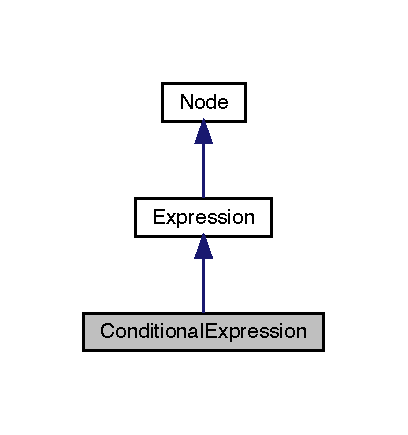
\includegraphics[width=196pt]{struct_conditional_expression__inherit__graph}
\end{center}
\end{figure}


Collaboration diagram for Conditional\+Expression\+:\nopagebreak
\begin{figure}[H]
\begin{center}
\leavevmode
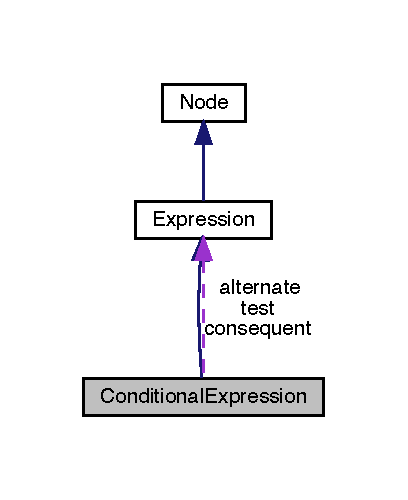
\includegraphics[width=196pt]{struct_conditional_expression__coll__graph}
\end{center}
\end{figure}
\subsection*{Public Member Functions}
\begin{DoxyCompactItemize}
\item 
\hyperlink{struct_conditional_expression_a37e1422b06b5533f67a85ceb92e9ae1e}{Conditional\+Expression} (\hyperlink{struct_expression}{Expression} $\ast$\hyperlink{struct_conditional_expression_a7bfe134769078a10eecccabba7405cc2}{test}, \hyperlink{struct_expression}{Expression} $\ast$\hyperlink{struct_conditional_expression_ac129a280df90c129183ec955f4e50ed0}{consequent}, \hyperlink{struct_expression}{Expression} $\ast$\hyperlink{struct_conditional_expression_aed7b09dab98000c8542d6353eefd8dac}{alternate})
\item 
void \hyperlink{struct_conditional_expression_af3883c99eba0226e3fbd424a672bcf7b}{accept} (\hyperlink{struct_visitor}{Visitor} \&visitor) const override
\end{DoxyCompactItemize}
\subsection*{Public Attributes}
\begin{DoxyCompactItemize}
\item 
\hyperlink{struct_expression}{Expression} $\ast$ \hyperlink{struct_conditional_expression_a7bfe134769078a10eecccabba7405cc2}{test}
\item 
\hyperlink{struct_expression}{Expression} $\ast$ \hyperlink{struct_conditional_expression_ac129a280df90c129183ec955f4e50ed0}{consequent}
\item 
\hyperlink{struct_expression}{Expression} $\ast$ \hyperlink{struct_conditional_expression_aed7b09dab98000c8542d6353eefd8dac}{alternate}
\end{DoxyCompactItemize}


\subsection{Constructor \& Destructor Documentation}
\mbox{\Hypertarget{struct_conditional_expression_a37e1422b06b5533f67a85ceb92e9ae1e}\label{struct_conditional_expression_a37e1422b06b5533f67a85ceb92e9ae1e}} 
\index{Conditional\+Expression@{Conditional\+Expression}!Conditional\+Expression@{Conditional\+Expression}}
\index{Conditional\+Expression@{Conditional\+Expression}!Conditional\+Expression@{Conditional\+Expression}}
\subsubsection{\texorpdfstring{Conditional\+Expression()}{ConditionalExpression()}}
{\footnotesize\ttfamily Conditional\+Expression\+::\+Conditional\+Expression (\begin{DoxyParamCaption}\item[{\hyperlink{struct_expression}{Expression} $\ast$}]{test,  }\item[{\hyperlink{struct_expression}{Expression} $\ast$}]{consequent,  }\item[{\hyperlink{struct_expression}{Expression} $\ast$}]{alternate }\end{DoxyParamCaption})\hspace{0.3cm}{\ttfamily [inline]}}



\subsection{Member Function Documentation}
\mbox{\Hypertarget{struct_conditional_expression_af3883c99eba0226e3fbd424a672bcf7b}\label{struct_conditional_expression_af3883c99eba0226e3fbd424a672bcf7b}} 
\index{Conditional\+Expression@{Conditional\+Expression}!accept@{accept}}
\index{accept@{accept}!Conditional\+Expression@{Conditional\+Expression}}
\subsubsection{\texorpdfstring{accept()}{accept()}}
{\footnotesize\ttfamily void Conditional\+Expression\+::accept (\begin{DoxyParamCaption}\item[{\hyperlink{struct_visitor}{Visitor} \&}]{visitor }\end{DoxyParamCaption}) const\hspace{0.3cm}{\ttfamily [inline]}, {\ttfamily [override]}, {\ttfamily [virtual]}}



Implements \hyperlink{struct_node_a10bd7af968140bbf5fa461298a969c71}{Node}.



\subsection{Member Data Documentation}
\mbox{\Hypertarget{struct_conditional_expression_aed7b09dab98000c8542d6353eefd8dac}\label{struct_conditional_expression_aed7b09dab98000c8542d6353eefd8dac}} 
\index{Conditional\+Expression@{Conditional\+Expression}!alternate@{alternate}}
\index{alternate@{alternate}!Conditional\+Expression@{Conditional\+Expression}}
\subsubsection{\texorpdfstring{alternate}{alternate}}
{\footnotesize\ttfamily \hyperlink{struct_expression}{Expression}$\ast$ Conditional\+Expression\+::alternate}

\mbox{\Hypertarget{struct_conditional_expression_ac129a280df90c129183ec955f4e50ed0}\label{struct_conditional_expression_ac129a280df90c129183ec955f4e50ed0}} 
\index{Conditional\+Expression@{Conditional\+Expression}!consequent@{consequent}}
\index{consequent@{consequent}!Conditional\+Expression@{Conditional\+Expression}}
\subsubsection{\texorpdfstring{consequent}{consequent}}
{\footnotesize\ttfamily \hyperlink{struct_expression}{Expression}$\ast$ Conditional\+Expression\+::consequent}

\mbox{\Hypertarget{struct_conditional_expression_a7bfe134769078a10eecccabba7405cc2}\label{struct_conditional_expression_a7bfe134769078a10eecccabba7405cc2}} 
\index{Conditional\+Expression@{Conditional\+Expression}!test@{test}}
\index{test@{test}!Conditional\+Expression@{Conditional\+Expression}}
\subsubsection{\texorpdfstring{test}{test}}
{\footnotesize\ttfamily \hyperlink{struct_expression}{Expression}$\ast$ Conditional\+Expression\+::test}



The documentation for this struct was generated from the following file\+:\begin{DoxyCompactItemize}
\item 
src/\hyperlink{ast_8h}{ast.\+h}\end{DoxyCompactItemize}

\hypertarget{struct_catch_1_1_matchers_1_1_vector_1_1_contains_element_matcher}{}\section{Catch\+:\+:Matchers\+:\+:Vector\+:\+:Contains\+Element\+Matcher$<$ T $>$ Struct Template Reference}
\label{struct_catch_1_1_matchers_1_1_vector_1_1_contains_element_matcher}\index{Catch\+::\+Matchers\+::\+Vector\+::\+Contains\+Element\+Matcher$<$ T $>$@{Catch\+::\+Matchers\+::\+Vector\+::\+Contains\+Element\+Matcher$<$ T $>$}}


{\ttfamily \#include $<$catch.\+hpp$>$}



Inheritance diagram for Catch\+:\+:Matchers\+:\+:Vector\+:\+:Contains\+Element\+Matcher$<$ T $>$\+:
\nopagebreak
\begin{figure}[H]
\begin{center}
\leavevmode
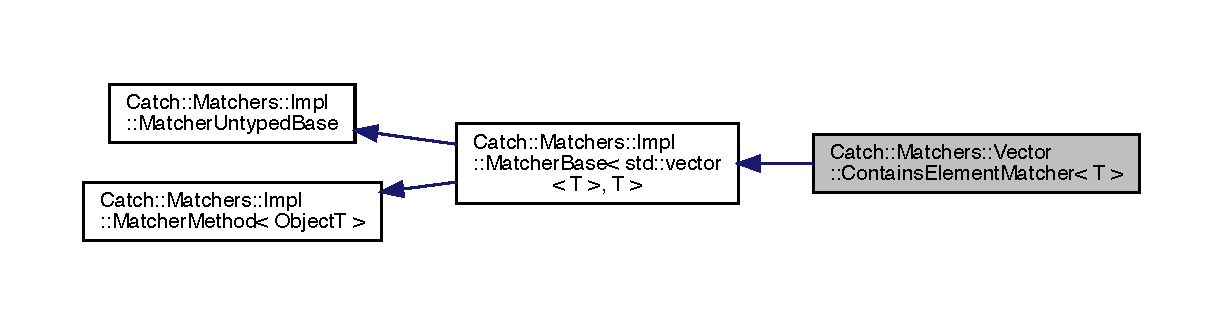
\includegraphics[width=350pt]{struct_catch_1_1_matchers_1_1_vector_1_1_contains_element_matcher__inherit__graph}
\end{center}
\end{figure}


Collaboration diagram for Catch\+:\+:Matchers\+:\+:Vector\+:\+:Contains\+Element\+Matcher$<$ T $>$\+:
\nopagebreak
\begin{figure}[H]
\begin{center}
\leavevmode
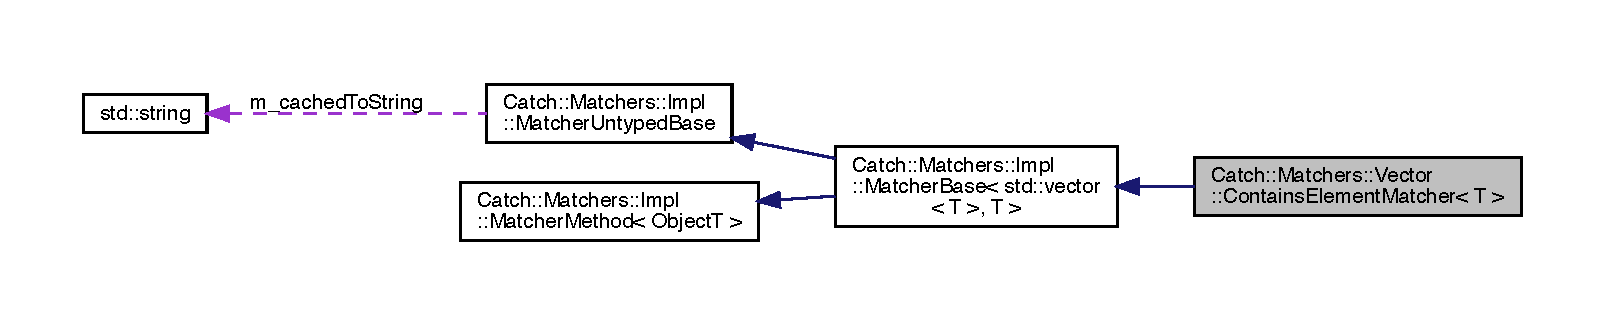
\includegraphics[width=350pt]{struct_catch_1_1_matchers_1_1_vector_1_1_contains_element_matcher__coll__graph}
\end{center}
\end{figure}
\subsection*{Public Member Functions}
\begin{DoxyCompactItemize}
\item 
\hyperlink{struct_catch_1_1_matchers_1_1_vector_1_1_contains_element_matcher_a6a05740b5d3f89fac8de84ac0cff7b93}{Contains\+Element\+Matcher} (T const \&comparator)
\item 
bool \hyperlink{struct_catch_1_1_matchers_1_1_vector_1_1_contains_element_matcher_a95fd99879bcfbe129898bef922c92c17}{match} (\textbf{ std\+::vector}$<$ T $>$ const \&v) const \hyperlink{catch_8hpp_a8ecdce4d3f57835f707915ae831eb847}{C\+A\+T\+C\+H\+\_\+\+O\+V\+E\+R\+R\+I\+DE}
\item 
virtual \textbf{ std\+::string} \hyperlink{struct_catch_1_1_matchers_1_1_vector_1_1_contains_element_matcher_a5a869772714dd045816707b74b217664}{describe} () const \hyperlink{catch_8hpp_a8ecdce4d3f57835f707915ae831eb847}{C\+A\+T\+C\+H\+\_\+\+O\+V\+E\+R\+R\+I\+DE}
\end{DoxyCompactItemize}
\subsection*{Public Attributes}
\begin{DoxyCompactItemize}
\item 
T const  \& \hyperlink{struct_catch_1_1_matchers_1_1_vector_1_1_contains_element_matcher_ab7eada6c4bbce1d21b44773262f9cb23}{m\+\_\+comparator}
\end{DoxyCompactItemize}
\subsection*{Additional Inherited Members}


\subsection{Constructor \& Destructor Documentation}
\mbox{\Hypertarget{struct_catch_1_1_matchers_1_1_vector_1_1_contains_element_matcher_a6a05740b5d3f89fac8de84ac0cff7b93}\label{struct_catch_1_1_matchers_1_1_vector_1_1_contains_element_matcher_a6a05740b5d3f89fac8de84ac0cff7b93}} 
\index{Catch\+::\+Matchers\+::\+Vector\+::\+Contains\+Element\+Matcher@{Catch\+::\+Matchers\+::\+Vector\+::\+Contains\+Element\+Matcher}!Contains\+Element\+Matcher@{Contains\+Element\+Matcher}}
\index{Contains\+Element\+Matcher@{Contains\+Element\+Matcher}!Catch\+::\+Matchers\+::\+Vector\+::\+Contains\+Element\+Matcher@{Catch\+::\+Matchers\+::\+Vector\+::\+Contains\+Element\+Matcher}}
\subsubsection{\texorpdfstring{Contains\+Element\+Matcher()}{ContainsElementMatcher()}}
{\footnotesize\ttfamily template$<$typename T $>$ \\
\hyperlink{struct_catch_1_1_matchers_1_1_vector_1_1_contains_element_matcher}{Catch\+::\+Matchers\+::\+Vector\+::\+Contains\+Element\+Matcher}$<$ T $>$\+::\hyperlink{struct_catch_1_1_matchers_1_1_vector_1_1_contains_element_matcher}{Contains\+Element\+Matcher} (\begin{DoxyParamCaption}\item[{T const \&}]{comparator }\end{DoxyParamCaption})\hspace{0.3cm}{\ttfamily [inline]}}



\subsection{Member Function Documentation}
\mbox{\Hypertarget{struct_catch_1_1_matchers_1_1_vector_1_1_contains_element_matcher_a5a869772714dd045816707b74b217664}\label{struct_catch_1_1_matchers_1_1_vector_1_1_contains_element_matcher_a5a869772714dd045816707b74b217664}} 
\index{Catch\+::\+Matchers\+::\+Vector\+::\+Contains\+Element\+Matcher@{Catch\+::\+Matchers\+::\+Vector\+::\+Contains\+Element\+Matcher}!describe@{describe}}
\index{describe@{describe}!Catch\+::\+Matchers\+::\+Vector\+::\+Contains\+Element\+Matcher@{Catch\+::\+Matchers\+::\+Vector\+::\+Contains\+Element\+Matcher}}
\subsubsection{\texorpdfstring{describe()}{describe()}}
{\footnotesize\ttfamily template$<$typename T $>$ \\
virtual \textbf{ std\+::string} \hyperlink{struct_catch_1_1_matchers_1_1_vector_1_1_contains_element_matcher}{Catch\+::\+Matchers\+::\+Vector\+::\+Contains\+Element\+Matcher}$<$ T $>$\+::describe (\begin{DoxyParamCaption}{ }\end{DoxyParamCaption}) const\hspace{0.3cm}{\ttfamily [inline]}, {\ttfamily [virtual]}}



Implements \hyperlink{class_catch_1_1_matchers_1_1_impl_1_1_matcher_untyped_base_a91d3a907dbfcbb596077df24f6e11fe2}{Catch\+::\+Matchers\+::\+Impl\+::\+Matcher\+Untyped\+Base}.

\mbox{\Hypertarget{struct_catch_1_1_matchers_1_1_vector_1_1_contains_element_matcher_a95fd99879bcfbe129898bef922c92c17}\label{struct_catch_1_1_matchers_1_1_vector_1_1_contains_element_matcher_a95fd99879bcfbe129898bef922c92c17}} 
\index{Catch\+::\+Matchers\+::\+Vector\+::\+Contains\+Element\+Matcher@{Catch\+::\+Matchers\+::\+Vector\+::\+Contains\+Element\+Matcher}!match@{match}}
\index{match@{match}!Catch\+::\+Matchers\+::\+Vector\+::\+Contains\+Element\+Matcher@{Catch\+::\+Matchers\+::\+Vector\+::\+Contains\+Element\+Matcher}}
\subsubsection{\texorpdfstring{match()}{match()}}
{\footnotesize\ttfamily template$<$typename T $>$ \\
bool \hyperlink{struct_catch_1_1_matchers_1_1_vector_1_1_contains_element_matcher}{Catch\+::\+Matchers\+::\+Vector\+::\+Contains\+Element\+Matcher}$<$ T $>$\+::match (\begin{DoxyParamCaption}\item[{\textbf{ std\+::vector}$<$ T $>$ const \&}]{v }\end{DoxyParamCaption}) const\hspace{0.3cm}{\ttfamily [inline]}}



\subsection{Member Data Documentation}
\mbox{\Hypertarget{struct_catch_1_1_matchers_1_1_vector_1_1_contains_element_matcher_ab7eada6c4bbce1d21b44773262f9cb23}\label{struct_catch_1_1_matchers_1_1_vector_1_1_contains_element_matcher_ab7eada6c4bbce1d21b44773262f9cb23}} 
\index{Catch\+::\+Matchers\+::\+Vector\+::\+Contains\+Element\+Matcher@{Catch\+::\+Matchers\+::\+Vector\+::\+Contains\+Element\+Matcher}!m\+\_\+comparator@{m\+\_\+comparator}}
\index{m\+\_\+comparator@{m\+\_\+comparator}!Catch\+::\+Matchers\+::\+Vector\+::\+Contains\+Element\+Matcher@{Catch\+::\+Matchers\+::\+Vector\+::\+Contains\+Element\+Matcher}}
\subsubsection{\texorpdfstring{m\+\_\+comparator}{m\_comparator}}
{\footnotesize\ttfamily template$<$typename T $>$ \\
T const\& \hyperlink{struct_catch_1_1_matchers_1_1_vector_1_1_contains_element_matcher}{Catch\+::\+Matchers\+::\+Vector\+::\+Contains\+Element\+Matcher}$<$ T $>$\+::m\+\_\+comparator}



The documentation for this struct was generated from the following file\+:\begin{DoxyCompactItemize}
\item 
src/\hyperlink{catch_8hpp}{catch.\+hpp}\end{DoxyCompactItemize}

\hypertarget{struct_catch_1_1_matchers_1_1_std_string_1_1_contains_matcher}{}\section{Catch\+:\+:Matchers\+:\+:Std\+String\+:\+:Contains\+Matcher Struct Reference}
\label{struct_catch_1_1_matchers_1_1_std_string_1_1_contains_matcher}\index{Catch\+::\+Matchers\+::\+Std\+String\+::\+Contains\+Matcher@{Catch\+::\+Matchers\+::\+Std\+String\+::\+Contains\+Matcher}}


{\ttfamily \#include $<$catch.\+hpp$>$}



Inheritance diagram for Catch\+:\+:Matchers\+:\+:Std\+String\+:\+:Contains\+Matcher\+:
\nopagebreak
\begin{figure}[H]
\begin{center}
\leavevmode
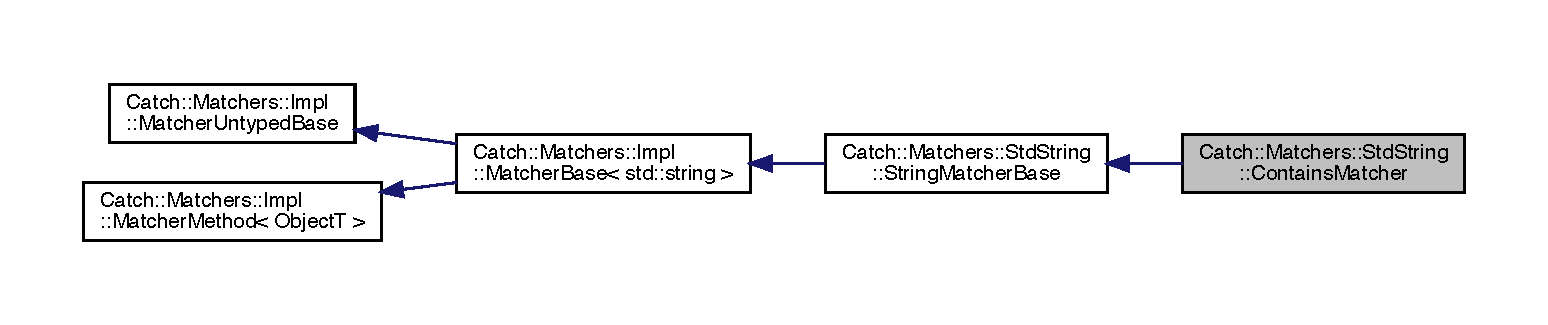
\includegraphics[width=350pt]{struct_catch_1_1_matchers_1_1_std_string_1_1_contains_matcher__inherit__graph}
\end{center}
\end{figure}


Collaboration diagram for Catch\+:\+:Matchers\+:\+:Std\+String\+:\+:Contains\+Matcher\+:
\nopagebreak
\begin{figure}[H]
\begin{center}
\leavevmode
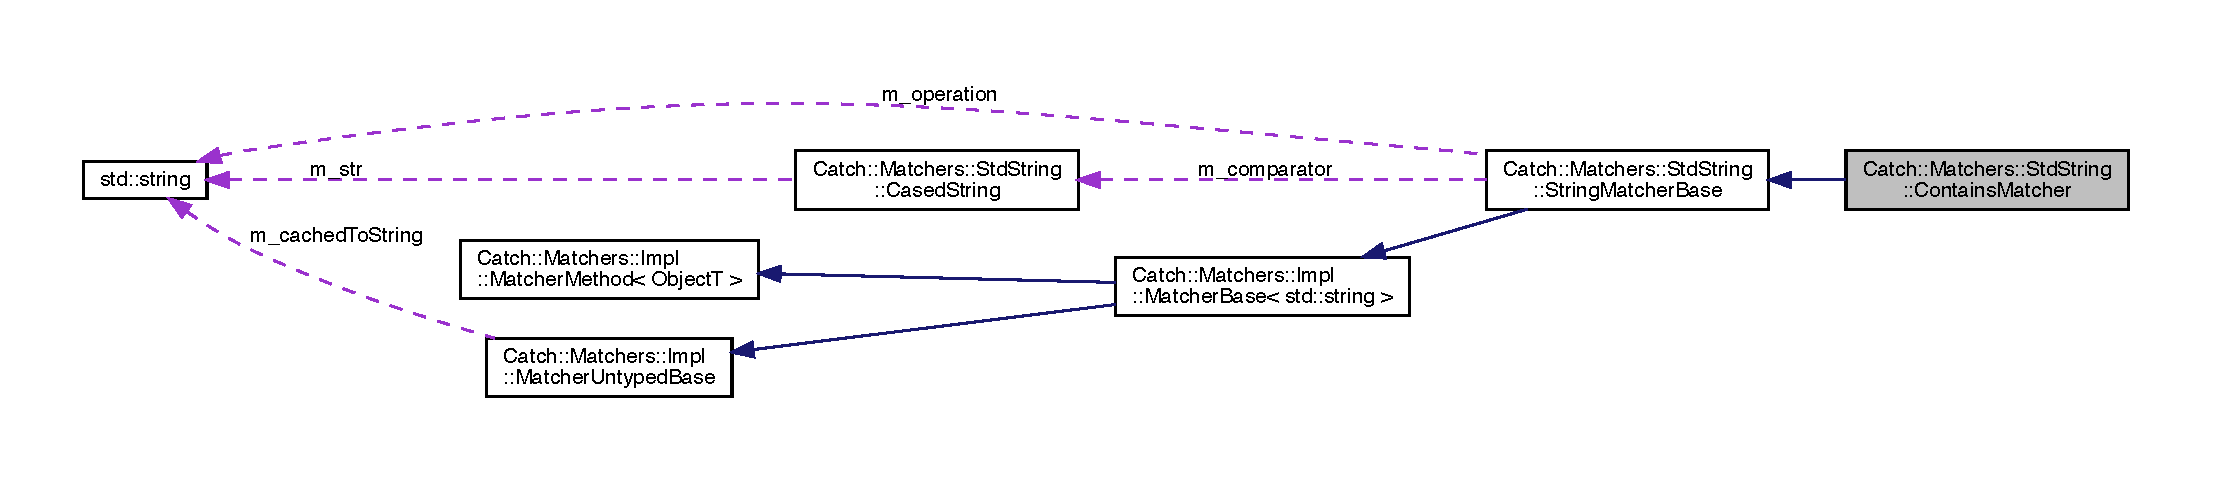
\includegraphics[width=350pt]{struct_catch_1_1_matchers_1_1_std_string_1_1_contains_matcher__coll__graph}
\end{center}
\end{figure}
\subsection*{Public Member Functions}
\begin{DoxyCompactItemize}
\item 
\hyperlink{struct_catch_1_1_matchers_1_1_std_string_1_1_contains_matcher_acc892883c8409e34b28c9b39d4ef1fe3}{Contains\+Matcher} (\hyperlink{struct_catch_1_1_matchers_1_1_std_string_1_1_cased_string}{Cased\+String} const \&comparator)
\item 
virtual bool \hyperlink{struct_catch_1_1_matchers_1_1_std_string_1_1_contains_matcher_ae4d567347fa563e365f1044f29ab1042}{match} (\textbf{ std\+::string} const \&source) const \hyperlink{catch_8hpp_a8ecdce4d3f57835f707915ae831eb847}{C\+A\+T\+C\+H\+\_\+\+O\+V\+E\+R\+R\+I\+DE}
\end{DoxyCompactItemize}
\subsection*{Additional Inherited Members}


\subsection{Constructor \& Destructor Documentation}
\mbox{\Hypertarget{struct_catch_1_1_matchers_1_1_std_string_1_1_contains_matcher_acc892883c8409e34b28c9b39d4ef1fe3}\label{struct_catch_1_1_matchers_1_1_std_string_1_1_contains_matcher_acc892883c8409e34b28c9b39d4ef1fe3}} 
\index{Catch\+::\+Matchers\+::\+Std\+String\+::\+Contains\+Matcher@{Catch\+::\+Matchers\+::\+Std\+String\+::\+Contains\+Matcher}!Contains\+Matcher@{Contains\+Matcher}}
\index{Contains\+Matcher@{Contains\+Matcher}!Catch\+::\+Matchers\+::\+Std\+String\+::\+Contains\+Matcher@{Catch\+::\+Matchers\+::\+Std\+String\+::\+Contains\+Matcher}}
\subsubsection{\texorpdfstring{Contains\+Matcher()}{ContainsMatcher()}}
{\footnotesize\ttfamily Catch\+::\+Matchers\+::\+Std\+String\+::\+Contains\+Matcher\+::\+Contains\+Matcher (\begin{DoxyParamCaption}\item[{\hyperlink{struct_catch_1_1_matchers_1_1_std_string_1_1_cased_string}{Cased\+String} const \&}]{comparator }\end{DoxyParamCaption})}



\subsection{Member Function Documentation}
\mbox{\Hypertarget{struct_catch_1_1_matchers_1_1_std_string_1_1_contains_matcher_ae4d567347fa563e365f1044f29ab1042}\label{struct_catch_1_1_matchers_1_1_std_string_1_1_contains_matcher_ae4d567347fa563e365f1044f29ab1042}} 
\index{Catch\+::\+Matchers\+::\+Std\+String\+::\+Contains\+Matcher@{Catch\+::\+Matchers\+::\+Std\+String\+::\+Contains\+Matcher}!match@{match}}
\index{match@{match}!Catch\+::\+Matchers\+::\+Std\+String\+::\+Contains\+Matcher@{Catch\+::\+Matchers\+::\+Std\+String\+::\+Contains\+Matcher}}
\subsubsection{\texorpdfstring{match()}{match()}}
{\footnotesize\ttfamily virtual bool Catch\+::\+Matchers\+::\+Std\+String\+::\+Contains\+Matcher\+::match (\begin{DoxyParamCaption}\item[{\textbf{ std\+::string} const \&}]{source }\end{DoxyParamCaption}) const\hspace{0.3cm}{\ttfamily [virtual]}}



The documentation for this struct was generated from the following file\+:\begin{DoxyCompactItemize}
\item 
src/\hyperlink{catch_8hpp}{catch.\+hpp}\end{DoxyCompactItemize}

\hypertarget{struct_catch_1_1_matchers_1_1_vector_1_1_contains_matcher}{}\section{Catch\+:\+:Matchers\+:\+:Vector\+:\+:Contains\+Matcher$<$ T $>$ Struct Template Reference}
\label{struct_catch_1_1_matchers_1_1_vector_1_1_contains_matcher}\index{Catch\+::\+Matchers\+::\+Vector\+::\+Contains\+Matcher$<$ T $>$@{Catch\+::\+Matchers\+::\+Vector\+::\+Contains\+Matcher$<$ T $>$}}


{\ttfamily \#include $<$catch.\+hpp$>$}



Inheritance diagram for Catch\+:\+:Matchers\+:\+:Vector\+:\+:Contains\+Matcher$<$ T $>$\+:
\nopagebreak
\begin{figure}[H]
\begin{center}
\leavevmode
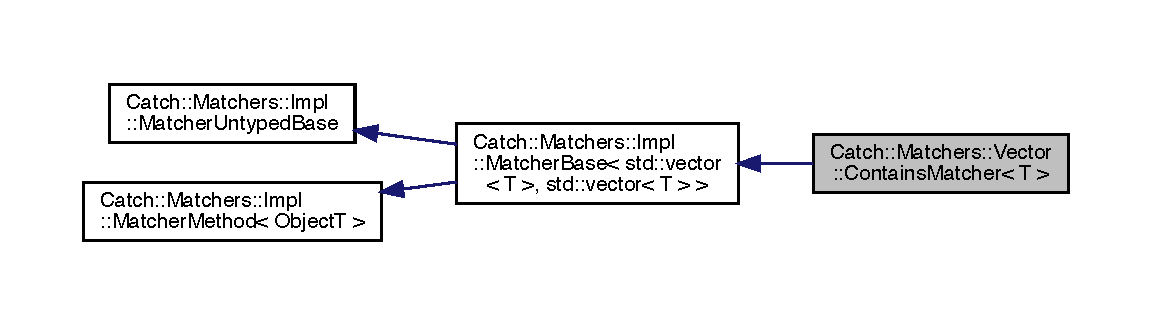
\includegraphics[width=350pt]{struct_catch_1_1_matchers_1_1_vector_1_1_contains_matcher__inherit__graph}
\end{center}
\end{figure}


Collaboration diagram for Catch\+:\+:Matchers\+:\+:Vector\+:\+:Contains\+Matcher$<$ T $>$\+:
\nopagebreak
\begin{figure}[H]
\begin{center}
\leavevmode
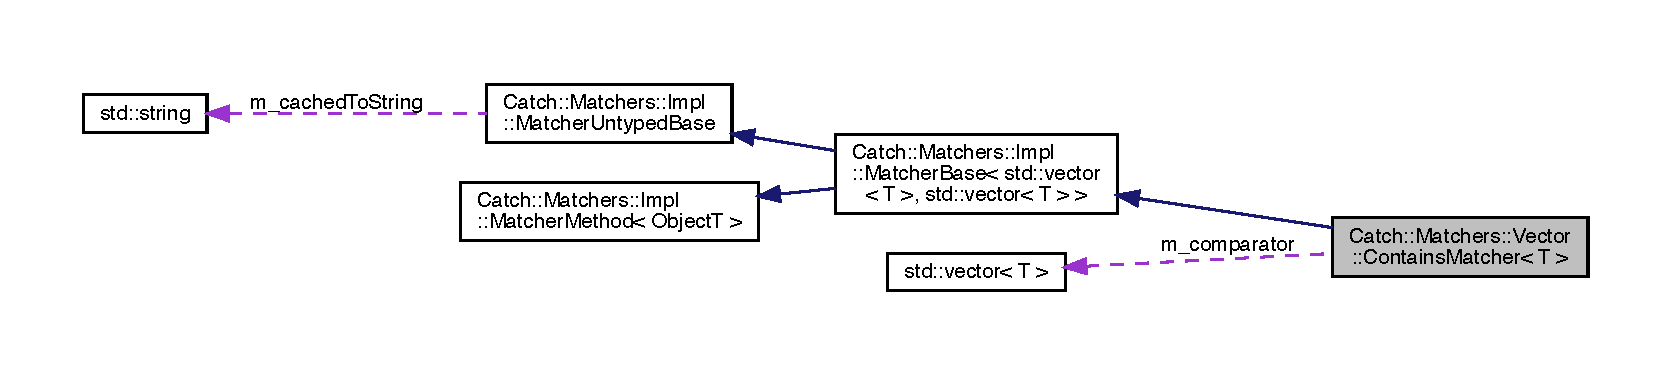
\includegraphics[width=350pt]{struct_catch_1_1_matchers_1_1_vector_1_1_contains_matcher__coll__graph}
\end{center}
\end{figure}
\subsection*{Public Member Functions}
\begin{DoxyCompactItemize}
\item 
\hyperlink{struct_catch_1_1_matchers_1_1_vector_1_1_contains_matcher_ad8e92c8399be6dce75bb5702cdfab700}{Contains\+Matcher} (\textbf{ std\+::vector}$<$ T $>$ const \&comparator)
\item 
bool \hyperlink{struct_catch_1_1_matchers_1_1_vector_1_1_contains_matcher_aba81516816a6796124dd4fe4843e7284}{match} (\textbf{ std\+::vector}$<$ T $>$ const \&v) const \hyperlink{catch_8hpp_a8ecdce4d3f57835f707915ae831eb847}{C\+A\+T\+C\+H\+\_\+\+O\+V\+E\+R\+R\+I\+DE}
\item 
virtual \textbf{ std\+::string} \hyperlink{struct_catch_1_1_matchers_1_1_vector_1_1_contains_matcher_add1a31f049cec89f980424ecdb7027ac}{describe} () const \hyperlink{catch_8hpp_a8ecdce4d3f57835f707915ae831eb847}{C\+A\+T\+C\+H\+\_\+\+O\+V\+E\+R\+R\+I\+DE}
\end{DoxyCompactItemize}
\subsection*{Public Attributes}
\begin{DoxyCompactItemize}
\item 
\textbf{ std\+::vector}$<$ T $>$ const  \& \hyperlink{struct_catch_1_1_matchers_1_1_vector_1_1_contains_matcher_a83d051166e4ed0d535219ad6ee99abb2}{m\+\_\+comparator}
\end{DoxyCompactItemize}
\subsection*{Additional Inherited Members}


\subsection{Constructor \& Destructor Documentation}
\mbox{\Hypertarget{struct_catch_1_1_matchers_1_1_vector_1_1_contains_matcher_ad8e92c8399be6dce75bb5702cdfab700}\label{struct_catch_1_1_matchers_1_1_vector_1_1_contains_matcher_ad8e92c8399be6dce75bb5702cdfab700}} 
\index{Catch\+::\+Matchers\+::\+Vector\+::\+Contains\+Matcher@{Catch\+::\+Matchers\+::\+Vector\+::\+Contains\+Matcher}!Contains\+Matcher@{Contains\+Matcher}}
\index{Contains\+Matcher@{Contains\+Matcher}!Catch\+::\+Matchers\+::\+Vector\+::\+Contains\+Matcher@{Catch\+::\+Matchers\+::\+Vector\+::\+Contains\+Matcher}}
\subsubsection{\texorpdfstring{Contains\+Matcher()}{ContainsMatcher()}}
{\footnotesize\ttfamily template$<$typename T $>$ \\
\hyperlink{struct_catch_1_1_matchers_1_1_vector_1_1_contains_matcher}{Catch\+::\+Matchers\+::\+Vector\+::\+Contains\+Matcher}$<$ T $>$\+::\hyperlink{struct_catch_1_1_matchers_1_1_vector_1_1_contains_matcher}{Contains\+Matcher} (\begin{DoxyParamCaption}\item[{\textbf{ std\+::vector}$<$ T $>$ const \&}]{comparator }\end{DoxyParamCaption})\hspace{0.3cm}{\ttfamily [inline]}}



\subsection{Member Function Documentation}
\mbox{\Hypertarget{struct_catch_1_1_matchers_1_1_vector_1_1_contains_matcher_add1a31f049cec89f980424ecdb7027ac}\label{struct_catch_1_1_matchers_1_1_vector_1_1_contains_matcher_add1a31f049cec89f980424ecdb7027ac}} 
\index{Catch\+::\+Matchers\+::\+Vector\+::\+Contains\+Matcher@{Catch\+::\+Matchers\+::\+Vector\+::\+Contains\+Matcher}!describe@{describe}}
\index{describe@{describe}!Catch\+::\+Matchers\+::\+Vector\+::\+Contains\+Matcher@{Catch\+::\+Matchers\+::\+Vector\+::\+Contains\+Matcher}}
\subsubsection{\texorpdfstring{describe()}{describe()}}
{\footnotesize\ttfamily template$<$typename T $>$ \\
virtual \textbf{ std\+::string} \hyperlink{struct_catch_1_1_matchers_1_1_vector_1_1_contains_matcher}{Catch\+::\+Matchers\+::\+Vector\+::\+Contains\+Matcher}$<$ T $>$\+::describe (\begin{DoxyParamCaption}{ }\end{DoxyParamCaption}) const\hspace{0.3cm}{\ttfamily [inline]}, {\ttfamily [virtual]}}



Implements \hyperlink{class_catch_1_1_matchers_1_1_impl_1_1_matcher_untyped_base_a91d3a907dbfcbb596077df24f6e11fe2}{Catch\+::\+Matchers\+::\+Impl\+::\+Matcher\+Untyped\+Base}.

\mbox{\Hypertarget{struct_catch_1_1_matchers_1_1_vector_1_1_contains_matcher_aba81516816a6796124dd4fe4843e7284}\label{struct_catch_1_1_matchers_1_1_vector_1_1_contains_matcher_aba81516816a6796124dd4fe4843e7284}} 
\index{Catch\+::\+Matchers\+::\+Vector\+::\+Contains\+Matcher@{Catch\+::\+Matchers\+::\+Vector\+::\+Contains\+Matcher}!match@{match}}
\index{match@{match}!Catch\+::\+Matchers\+::\+Vector\+::\+Contains\+Matcher@{Catch\+::\+Matchers\+::\+Vector\+::\+Contains\+Matcher}}
\subsubsection{\texorpdfstring{match()}{match()}}
{\footnotesize\ttfamily template$<$typename T $>$ \\
bool \hyperlink{struct_catch_1_1_matchers_1_1_vector_1_1_contains_matcher}{Catch\+::\+Matchers\+::\+Vector\+::\+Contains\+Matcher}$<$ T $>$\+::match (\begin{DoxyParamCaption}\item[{\textbf{ std\+::vector}$<$ T $>$ const \&}]{v }\end{DoxyParamCaption}) const\hspace{0.3cm}{\ttfamily [inline]}}



\subsection{Member Data Documentation}
\mbox{\Hypertarget{struct_catch_1_1_matchers_1_1_vector_1_1_contains_matcher_a83d051166e4ed0d535219ad6ee99abb2}\label{struct_catch_1_1_matchers_1_1_vector_1_1_contains_matcher_a83d051166e4ed0d535219ad6ee99abb2}} 
\index{Catch\+::\+Matchers\+::\+Vector\+::\+Contains\+Matcher@{Catch\+::\+Matchers\+::\+Vector\+::\+Contains\+Matcher}!m\+\_\+comparator@{m\+\_\+comparator}}
\index{m\+\_\+comparator@{m\+\_\+comparator}!Catch\+::\+Matchers\+::\+Vector\+::\+Contains\+Matcher@{Catch\+::\+Matchers\+::\+Vector\+::\+Contains\+Matcher}}
\subsubsection{\texorpdfstring{m\+\_\+comparator}{m\_comparator}}
{\footnotesize\ttfamily template$<$typename T $>$ \\
\textbf{ std\+::vector}$<$T$>$ const\& \hyperlink{struct_catch_1_1_matchers_1_1_vector_1_1_contains_matcher}{Catch\+::\+Matchers\+::\+Vector\+::\+Contains\+Matcher}$<$ T $>$\+::m\+\_\+comparator}



The documentation for this struct was generated from the following file\+:\begin{DoxyCompactItemize}
\item 
src/\hyperlink{catch_8hpp}{catch.\+hpp}\end{DoxyCompactItemize}

\hypertarget{struct_continue_statement}{}\section{Continue\+Statement Struct Reference}
\label{struct_continue_statement}\index{Continue\+Statement@{Continue\+Statement}}


{\ttfamily \#include $<$ast.\+h$>$}



Inheritance diagram for Continue\+Statement\+:\nopagebreak
\begin{figure}[H]
\begin{center}
\leavevmode
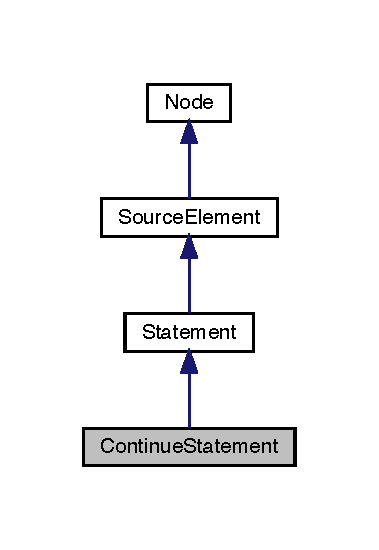
\includegraphics[width=182pt]{struct_continue_statement__inherit__graph}
\end{center}
\end{figure}


Collaboration diagram for Continue\+Statement\+:
\nopagebreak
\begin{figure}[H]
\begin{center}
\leavevmode
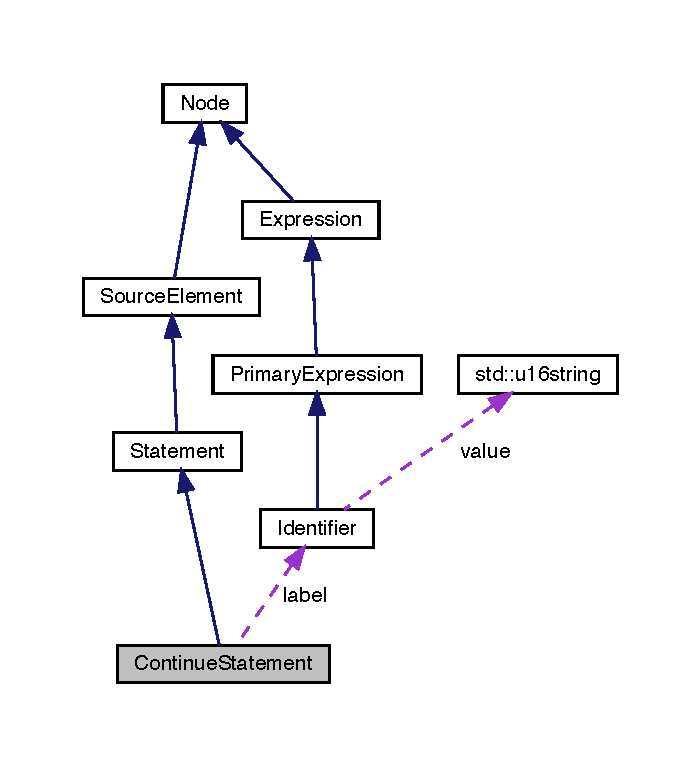
\includegraphics[width=247pt]{struct_continue_statement__coll__graph}
\end{center}
\end{figure}
\subsection*{Public Member Functions}
\begin{DoxyCompactItemize}
\item 
\hyperlink{struct_continue_statement_a45152addd01adf9e6d10c0af8505128c}{Continue\+Statement} (\hyperlink{struct_identifier}{Identifier} $\ast$\hyperlink{struct_continue_statement_a4bf8883a88736fa6ce4341e9029db194}{label}=nullptr)
\item 
void \hyperlink{struct_continue_statement_a9288fc77078160a2709a6329f1fe4838}{accept} (\hyperlink{struct_visitor}{Visitor} \&visitor) const override
\item 
const char $\ast$ \hyperlink{struct_continue_statement_a08b73034c5d273c3c4cbad00b252913f}{type} () const override
\end{DoxyCompactItemize}
\subsection*{Public Attributes}
\begin{DoxyCompactItemize}
\item 
\hyperlink{struct_identifier}{Identifier} $\ast$ \hyperlink{struct_continue_statement_a4bf8883a88736fa6ce4341e9029db194}{label}
\end{DoxyCompactItemize}


\subsection{Constructor \& Destructor Documentation}
\mbox{\Hypertarget{struct_continue_statement_a45152addd01adf9e6d10c0af8505128c}\label{struct_continue_statement_a45152addd01adf9e6d10c0af8505128c}} 
\index{Continue\+Statement@{Continue\+Statement}!Continue\+Statement@{Continue\+Statement}}
\index{Continue\+Statement@{Continue\+Statement}!Continue\+Statement@{Continue\+Statement}}
\subsubsection{\texorpdfstring{Continue\+Statement()}{ContinueStatement()}}
{\footnotesize\ttfamily Continue\+Statement\+::\+Continue\+Statement (\begin{DoxyParamCaption}\item[{\hyperlink{struct_identifier}{Identifier} $\ast$}]{label = {\ttfamily nullptr} }\end{DoxyParamCaption})\hspace{0.3cm}{\ttfamily [inline]}}



\subsection{Member Function Documentation}
\mbox{\Hypertarget{struct_continue_statement_a9288fc77078160a2709a6329f1fe4838}\label{struct_continue_statement_a9288fc77078160a2709a6329f1fe4838}} 
\index{Continue\+Statement@{Continue\+Statement}!accept@{accept}}
\index{accept@{accept}!Continue\+Statement@{Continue\+Statement}}
\subsubsection{\texorpdfstring{accept()}{accept()}}
{\footnotesize\ttfamily void Continue\+Statement\+::accept (\begin{DoxyParamCaption}\item[{\hyperlink{struct_visitor}{Visitor} \&}]{visitor }\end{DoxyParamCaption}) const\hspace{0.3cm}{\ttfamily [inline]}, {\ttfamily [override]}, {\ttfamily [virtual]}}



Implements \hyperlink{struct_node_a10bd7af968140bbf5fa461298a969c71}{Node}.

\mbox{\Hypertarget{struct_continue_statement_a08b73034c5d273c3c4cbad00b252913f}\label{struct_continue_statement_a08b73034c5d273c3c4cbad00b252913f}} 
\index{Continue\+Statement@{Continue\+Statement}!type@{type}}
\index{type@{type}!Continue\+Statement@{Continue\+Statement}}
\subsubsection{\texorpdfstring{type()}{type()}}
{\footnotesize\ttfamily const char$\ast$ Continue\+Statement\+::type (\begin{DoxyParamCaption}{ }\end{DoxyParamCaption}) const\hspace{0.3cm}{\ttfamily [inline]}, {\ttfamily [override]}, {\ttfamily [virtual]}}



Implements \hyperlink{struct_node_a82f29420d0a38efcc370352528e94e9b}{Node}.



\subsection{Member Data Documentation}
\mbox{\Hypertarget{struct_continue_statement_a4bf8883a88736fa6ce4341e9029db194}\label{struct_continue_statement_a4bf8883a88736fa6ce4341e9029db194}} 
\index{Continue\+Statement@{Continue\+Statement}!label@{label}}
\index{label@{label}!Continue\+Statement@{Continue\+Statement}}
\subsubsection{\texorpdfstring{label}{label}}
{\footnotesize\ttfamily \hyperlink{struct_identifier}{Identifier}$\ast$ Continue\+Statement\+::label}



The documentation for this struct was generated from the following file\+:\begin{DoxyCompactItemize}
\item 
src/\hyperlink{ast_8h}{ast.\+h}\end{DoxyCompactItemize}

\hypertarget{struct_catch_1_1_copyable_stream}{}\section{Catch\+:\+:Copyable\+Stream Struct Reference}
\label{struct_catch_1_1_copyable_stream}\index{Catch\+::\+Copyable\+Stream@{Catch\+::\+Copyable\+Stream}}


{\ttfamily \#include $<$catch.\+hpp$>$}



Collaboration diagram for Catch\+:\+:Copyable\+Stream\+:
\nopagebreak
\begin{figure}[H]
\begin{center}
\leavevmode
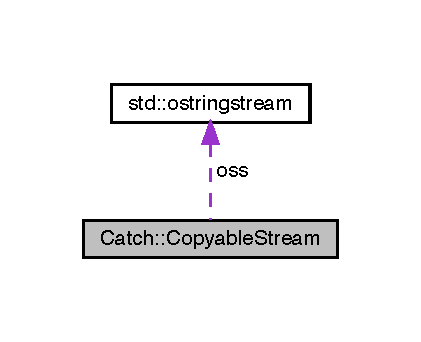
\includegraphics[width=202pt]{struct_catch_1_1_copyable_stream__coll__graph}
\end{center}
\end{figure}
\subsection*{Public Member Functions}
\begin{DoxyCompactItemize}
\item 
\hyperlink{struct_catch_1_1_copyable_stream_a5a61d0da675ae00cd46efaef4c445cdd}{Copyable\+Stream} ()
\item 
\hyperlink{struct_catch_1_1_copyable_stream_a0e72dc16240653f52c17106f4bf34da8}{Copyable\+Stream} (\hyperlink{struct_catch_1_1_copyable_stream}{Copyable\+Stream} const \&other)
\item 
\hyperlink{struct_catch_1_1_copyable_stream}{Copyable\+Stream} \& \hyperlink{struct_catch_1_1_copyable_stream_a1760fa29b38011c5845171260bec0966}{operator=} (\hyperlink{struct_catch_1_1_copyable_stream}{Copyable\+Stream} const \&other)
\end{DoxyCompactItemize}
\subsection*{Public Attributes}
\begin{DoxyCompactItemize}
\item 
\textbf{ std\+::ostringstream} \hyperlink{struct_catch_1_1_copyable_stream_ae123fb4d673e7d7a13a3c5f6bc5d426c}{oss}
\end{DoxyCompactItemize}


\subsection{Constructor \& Destructor Documentation}
\mbox{\Hypertarget{struct_catch_1_1_copyable_stream_a5a61d0da675ae00cd46efaef4c445cdd}\label{struct_catch_1_1_copyable_stream_a5a61d0da675ae00cd46efaef4c445cdd}} 
\index{Catch\+::\+Copyable\+Stream@{Catch\+::\+Copyable\+Stream}!Copyable\+Stream@{Copyable\+Stream}}
\index{Copyable\+Stream@{Copyable\+Stream}!Catch\+::\+Copyable\+Stream@{Catch\+::\+Copyable\+Stream}}
\subsubsection{\texorpdfstring{Copyable\+Stream()}{CopyableStream()}\hspace{0.1cm}{\footnotesize\ttfamily [1/2]}}
{\footnotesize\ttfamily Catch\+::\+Copyable\+Stream\+::\+Copyable\+Stream (\begin{DoxyParamCaption}{ }\end{DoxyParamCaption})\hspace{0.3cm}{\ttfamily [inline]}}

\mbox{\Hypertarget{struct_catch_1_1_copyable_stream_a0e72dc16240653f52c17106f4bf34da8}\label{struct_catch_1_1_copyable_stream_a0e72dc16240653f52c17106f4bf34da8}} 
\index{Catch\+::\+Copyable\+Stream@{Catch\+::\+Copyable\+Stream}!Copyable\+Stream@{Copyable\+Stream}}
\index{Copyable\+Stream@{Copyable\+Stream}!Catch\+::\+Copyable\+Stream@{Catch\+::\+Copyable\+Stream}}
\subsubsection{\texorpdfstring{Copyable\+Stream()}{CopyableStream()}\hspace{0.1cm}{\footnotesize\ttfamily [2/2]}}
{\footnotesize\ttfamily Catch\+::\+Copyable\+Stream\+::\+Copyable\+Stream (\begin{DoxyParamCaption}\item[{\hyperlink{struct_catch_1_1_copyable_stream}{Copyable\+Stream} const \&}]{other }\end{DoxyParamCaption})\hspace{0.3cm}{\ttfamily [inline]}}



\subsection{Member Function Documentation}
\mbox{\Hypertarget{struct_catch_1_1_copyable_stream_a1760fa29b38011c5845171260bec0966}\label{struct_catch_1_1_copyable_stream_a1760fa29b38011c5845171260bec0966}} 
\index{Catch\+::\+Copyable\+Stream@{Catch\+::\+Copyable\+Stream}!operator=@{operator=}}
\index{operator=@{operator=}!Catch\+::\+Copyable\+Stream@{Catch\+::\+Copyable\+Stream}}
\subsubsection{\texorpdfstring{operator=()}{operator=()}}
{\footnotesize\ttfamily \hyperlink{struct_catch_1_1_copyable_stream}{Copyable\+Stream}\& Catch\+::\+Copyable\+Stream\+::operator= (\begin{DoxyParamCaption}\item[{\hyperlink{struct_catch_1_1_copyable_stream}{Copyable\+Stream} const \&}]{other }\end{DoxyParamCaption})\hspace{0.3cm}{\ttfamily [inline]}}



\subsection{Member Data Documentation}
\mbox{\Hypertarget{struct_catch_1_1_copyable_stream_ae123fb4d673e7d7a13a3c5f6bc5d426c}\label{struct_catch_1_1_copyable_stream_ae123fb4d673e7d7a13a3c5f6bc5d426c}} 
\index{Catch\+::\+Copyable\+Stream@{Catch\+::\+Copyable\+Stream}!oss@{oss}}
\index{oss@{oss}!Catch\+::\+Copyable\+Stream@{Catch\+::\+Copyable\+Stream}}
\subsubsection{\texorpdfstring{oss}{oss}}
{\footnotesize\ttfamily \textbf{ std\+::ostringstream} Catch\+::\+Copyable\+Stream\+::oss}



The documentation for this struct was generated from the following file\+:\begin{DoxyCompactItemize}
\item 
src/\hyperlink{catch_8hpp}{catch.\+hpp}\end{DoxyCompactItemize}

\hypertarget{struct_catch_1_1_counts}{}\section{Catch\+:\+:Counts Struct Reference}
\label{struct_catch_1_1_counts}\index{Catch\+::\+Counts@{Catch\+::\+Counts}}


{\ttfamily \#include $<$catch.\+hpp$>$}



Collaboration diagram for Catch\+:\+:Counts\+:
\nopagebreak
\begin{figure}[H]
\begin{center}
\leavevmode
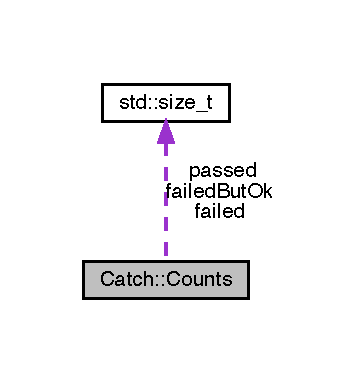
\includegraphics[width=171pt]{struct_catch_1_1_counts__coll__graph}
\end{center}
\end{figure}
\subsection*{Public Member Functions}
\begin{DoxyCompactItemize}
\item 
\hyperlink{struct_catch_1_1_counts_aab9092ce70d4b0179cc743555d2fc39b}{Counts} ()
\item 
\hyperlink{struct_catch_1_1_counts}{Counts} \hyperlink{struct_catch_1_1_counts_aaa10666f559057e3e860d2a5a6fae4c4}{operator-\/} (\hyperlink{struct_catch_1_1_counts}{Counts} const \&other) const
\item 
\hyperlink{struct_catch_1_1_counts}{Counts} \& \hyperlink{struct_catch_1_1_counts_a322a89475cd2cc039140ef371e973677}{operator+=} (\hyperlink{struct_catch_1_1_counts}{Counts} const \&other)
\item 
\textbf{ std\+::size\+\_\+t} \hyperlink{struct_catch_1_1_counts_a94f969c09cf52d1339c085c9603cd1d3}{total} () const
\item 
bool \hyperlink{struct_catch_1_1_counts_a84999490e0ecaa3de5e121bf48eda1b3}{all\+Passed} () const
\item 
bool \hyperlink{struct_catch_1_1_counts_a33bd996e016030155b99fe1c51c08991}{all\+Ok} () const
\end{DoxyCompactItemize}
\subsection*{Public Attributes}
\begin{DoxyCompactItemize}
\item 
\textbf{ std\+::size\+\_\+t} \hyperlink{struct_catch_1_1_counts_ad28daaf3de28006400208b6dd0c631e6}{passed}
\item 
\textbf{ std\+::size\+\_\+t} \hyperlink{struct_catch_1_1_counts_a19982a3817a3bc2c07f0290e71f497a3}{failed}
\item 
\textbf{ std\+::size\+\_\+t} \hyperlink{struct_catch_1_1_counts_ac090973a2ff51394cd452718e75c073e}{failed\+But\+Ok}
\end{DoxyCompactItemize}


\subsection{Constructor \& Destructor Documentation}
\mbox{\Hypertarget{struct_catch_1_1_counts_aab9092ce70d4b0179cc743555d2fc39b}\label{struct_catch_1_1_counts_aab9092ce70d4b0179cc743555d2fc39b}} 
\index{Catch\+::\+Counts@{Catch\+::\+Counts}!Counts@{Counts}}
\index{Counts@{Counts}!Catch\+::\+Counts@{Catch\+::\+Counts}}
\subsubsection{\texorpdfstring{Counts()}{Counts()}}
{\footnotesize\ttfamily Catch\+::\+Counts\+::\+Counts (\begin{DoxyParamCaption}{ }\end{DoxyParamCaption})\hspace{0.3cm}{\ttfamily [inline]}}



\subsection{Member Function Documentation}
\mbox{\Hypertarget{struct_catch_1_1_counts_a33bd996e016030155b99fe1c51c08991}\label{struct_catch_1_1_counts_a33bd996e016030155b99fe1c51c08991}} 
\index{Catch\+::\+Counts@{Catch\+::\+Counts}!all\+Ok@{all\+Ok}}
\index{all\+Ok@{all\+Ok}!Catch\+::\+Counts@{Catch\+::\+Counts}}
\subsubsection{\texorpdfstring{all\+Ok()}{allOk()}}
{\footnotesize\ttfamily bool Catch\+::\+Counts\+::all\+Ok (\begin{DoxyParamCaption}{ }\end{DoxyParamCaption}) const\hspace{0.3cm}{\ttfamily [inline]}}

\mbox{\Hypertarget{struct_catch_1_1_counts_a84999490e0ecaa3de5e121bf48eda1b3}\label{struct_catch_1_1_counts_a84999490e0ecaa3de5e121bf48eda1b3}} 
\index{Catch\+::\+Counts@{Catch\+::\+Counts}!all\+Passed@{all\+Passed}}
\index{all\+Passed@{all\+Passed}!Catch\+::\+Counts@{Catch\+::\+Counts}}
\subsubsection{\texorpdfstring{all\+Passed()}{allPassed()}}
{\footnotesize\ttfamily bool Catch\+::\+Counts\+::all\+Passed (\begin{DoxyParamCaption}{ }\end{DoxyParamCaption}) const\hspace{0.3cm}{\ttfamily [inline]}}

\mbox{\Hypertarget{struct_catch_1_1_counts_a322a89475cd2cc039140ef371e973677}\label{struct_catch_1_1_counts_a322a89475cd2cc039140ef371e973677}} 
\index{Catch\+::\+Counts@{Catch\+::\+Counts}!operator+=@{operator+=}}
\index{operator+=@{operator+=}!Catch\+::\+Counts@{Catch\+::\+Counts}}
\subsubsection{\texorpdfstring{operator+=()}{operator+=()}}
{\footnotesize\ttfamily \hyperlink{struct_catch_1_1_counts}{Counts}\& Catch\+::\+Counts\+::operator+= (\begin{DoxyParamCaption}\item[{\hyperlink{struct_catch_1_1_counts}{Counts} const \&}]{other }\end{DoxyParamCaption})\hspace{0.3cm}{\ttfamily [inline]}}

\mbox{\Hypertarget{struct_catch_1_1_counts_aaa10666f559057e3e860d2a5a6fae4c4}\label{struct_catch_1_1_counts_aaa10666f559057e3e860d2a5a6fae4c4}} 
\index{Catch\+::\+Counts@{Catch\+::\+Counts}!operator-\/@{operator-\/}}
\index{operator-\/@{operator-\/}!Catch\+::\+Counts@{Catch\+::\+Counts}}
\subsubsection{\texorpdfstring{operator-\/()}{operator-()}}
{\footnotesize\ttfamily \hyperlink{struct_catch_1_1_counts}{Counts} Catch\+::\+Counts\+::operator-\/ (\begin{DoxyParamCaption}\item[{\hyperlink{struct_catch_1_1_counts}{Counts} const \&}]{other }\end{DoxyParamCaption}) const\hspace{0.3cm}{\ttfamily [inline]}}

\mbox{\Hypertarget{struct_catch_1_1_counts_a94f969c09cf52d1339c085c9603cd1d3}\label{struct_catch_1_1_counts_a94f969c09cf52d1339c085c9603cd1d3}} 
\index{Catch\+::\+Counts@{Catch\+::\+Counts}!total@{total}}
\index{total@{total}!Catch\+::\+Counts@{Catch\+::\+Counts}}
\subsubsection{\texorpdfstring{total()}{total()}}
{\footnotesize\ttfamily \textbf{ std\+::size\+\_\+t} Catch\+::\+Counts\+::total (\begin{DoxyParamCaption}{ }\end{DoxyParamCaption}) const\hspace{0.3cm}{\ttfamily [inline]}}



\subsection{Member Data Documentation}
\mbox{\Hypertarget{struct_catch_1_1_counts_a19982a3817a3bc2c07f0290e71f497a3}\label{struct_catch_1_1_counts_a19982a3817a3bc2c07f0290e71f497a3}} 
\index{Catch\+::\+Counts@{Catch\+::\+Counts}!failed@{failed}}
\index{failed@{failed}!Catch\+::\+Counts@{Catch\+::\+Counts}}
\subsubsection{\texorpdfstring{failed}{failed}}
{\footnotesize\ttfamily \textbf{ std\+::size\+\_\+t} Catch\+::\+Counts\+::failed}

\mbox{\Hypertarget{struct_catch_1_1_counts_ac090973a2ff51394cd452718e75c073e}\label{struct_catch_1_1_counts_ac090973a2ff51394cd452718e75c073e}} 
\index{Catch\+::\+Counts@{Catch\+::\+Counts}!failed\+But\+Ok@{failed\+But\+Ok}}
\index{failed\+But\+Ok@{failed\+But\+Ok}!Catch\+::\+Counts@{Catch\+::\+Counts}}
\subsubsection{\texorpdfstring{failed\+But\+Ok}{failedButOk}}
{\footnotesize\ttfamily \textbf{ std\+::size\+\_\+t} Catch\+::\+Counts\+::failed\+But\+Ok}

\mbox{\Hypertarget{struct_catch_1_1_counts_ad28daaf3de28006400208b6dd0c631e6}\label{struct_catch_1_1_counts_ad28daaf3de28006400208b6dd0c631e6}} 
\index{Catch\+::\+Counts@{Catch\+::\+Counts}!passed@{passed}}
\index{passed@{passed}!Catch\+::\+Counts@{Catch\+::\+Counts}}
\subsubsection{\texorpdfstring{passed}{passed}}
{\footnotesize\ttfamily \textbf{ std\+::size\+\_\+t} Catch\+::\+Counts\+::passed}



The documentation for this struct was generated from the following file\+:\begin{DoxyCompactItemize}
\item 
src/\hyperlink{catch_8hpp}{catch.\+hpp}\end{DoxyCompactItemize}

\hypertarget{struct_debugger_statement}{}\section{Debugger\+Statement Struct Reference}
\label{struct_debugger_statement}\index{Debugger\+Statement@{Debugger\+Statement}}


{\ttfamily \#include $<$ast.\+h$>$}



Inheritance diagram for Debugger\+Statement\+:\nopagebreak
\begin{figure}[H]
\begin{center}
\leavevmode
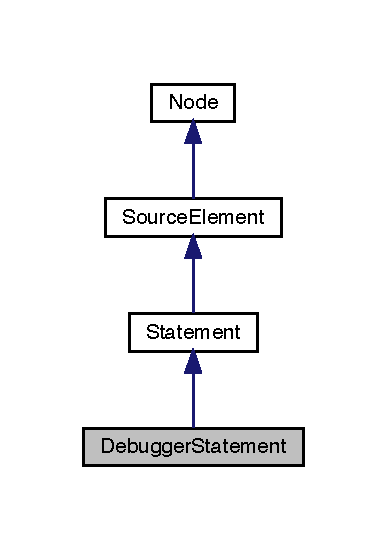
\includegraphics[width=186pt]{struct_debugger_statement__inherit__graph}
\end{center}
\end{figure}


Collaboration diagram for Debugger\+Statement\+:\nopagebreak
\begin{figure}[H]
\begin{center}
\leavevmode
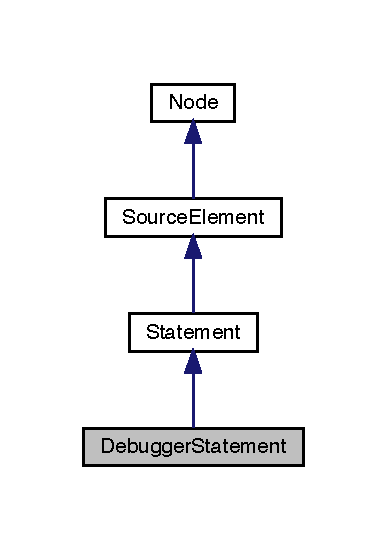
\includegraphics[width=186pt]{struct_debugger_statement__coll__graph}
\end{center}
\end{figure}
\subsection*{Public Member Functions}
\begin{DoxyCompactItemize}
\item 
void \hyperlink{struct_debugger_statement_adb69027b0b27e1a8f74f4ddea5957799}{accept} (\hyperlink{struct_visitor}{Visitor} \&visitor) const override
\item 
const char $\ast$ \hyperlink{struct_debugger_statement_a3484d4e9900b72324bf5eb55da9492dd}{type} () const override
\end{DoxyCompactItemize}


\subsection{Member Function Documentation}
\mbox{\Hypertarget{struct_debugger_statement_adb69027b0b27e1a8f74f4ddea5957799}\label{struct_debugger_statement_adb69027b0b27e1a8f74f4ddea5957799}} 
\index{Debugger\+Statement@{Debugger\+Statement}!accept@{accept}}
\index{accept@{accept}!Debugger\+Statement@{Debugger\+Statement}}
\subsubsection{\texorpdfstring{accept()}{accept()}}
{\footnotesize\ttfamily void Debugger\+Statement\+::accept (\begin{DoxyParamCaption}\item[{\hyperlink{struct_visitor}{Visitor} \&}]{visitor }\end{DoxyParamCaption}) const\hspace{0.3cm}{\ttfamily [inline]}, {\ttfamily [override]}, {\ttfamily [virtual]}}



Implements \hyperlink{struct_node_a10bd7af968140bbf5fa461298a969c71}{Node}.

\mbox{\Hypertarget{struct_debugger_statement_a3484d4e9900b72324bf5eb55da9492dd}\label{struct_debugger_statement_a3484d4e9900b72324bf5eb55da9492dd}} 
\index{Debugger\+Statement@{Debugger\+Statement}!type@{type}}
\index{type@{type}!Debugger\+Statement@{Debugger\+Statement}}
\subsubsection{\texorpdfstring{type()}{type()}}
{\footnotesize\ttfamily const char$\ast$ Debugger\+Statement\+::type (\begin{DoxyParamCaption}{ }\end{DoxyParamCaption}) const\hspace{0.3cm}{\ttfamily [inline]}, {\ttfamily [override]}, {\ttfamily [virtual]}}



Implements \hyperlink{struct_node_a82f29420d0a38efcc370352528e94e9b}{Node}.



The documentation for this struct was generated from the following file\+:\begin{DoxyCompactItemize}
\item 
src/\hyperlink{ast_8h}{ast.\+h}\end{DoxyCompactItemize}

\hypertarget{struct_token_1_1_debug_info}{}\section{Token\+:\+:Debug\+Info Struct Reference}
\label{struct_token_1_1_debug_info}\index{Token\+::\+Debug\+Info@{Token\+::\+Debug\+Info}}


{\ttfamily \#include $<$token.\+h$>$}

\subsection*{Public Member Functions}
\begin{DoxyCompactItemize}
\item 
virtual \textbf{ std\+::string} \hyperlink{struct_token_1_1_debug_info_a4d66aa65422c236198bbcc616bba250f}{syntax\+\_\+error\+\_\+at} () const =0
\item 
virtual \textbf{ std\+::string} \hyperlink{struct_token_1_1_debug_info_a0860d9b875240dafa0e00756d27e55bb}{loc} () const =0
\end{DoxyCompactItemize}


\subsection{Member Function Documentation}
\mbox{\Hypertarget{struct_token_1_1_debug_info_a0860d9b875240dafa0e00756d27e55bb}\label{struct_token_1_1_debug_info_a0860d9b875240dafa0e00756d27e55bb}} 
\index{Token\+::\+Debug\+Info@{Token\+::\+Debug\+Info}!loc@{loc}}
\index{loc@{loc}!Token\+::\+Debug\+Info@{Token\+::\+Debug\+Info}}
\subsubsection{\texorpdfstring{loc()}{loc()}}
{\footnotesize\ttfamily virtual \textbf{ std\+::string} Token\+::\+Debug\+Info\+::loc (\begin{DoxyParamCaption}{ }\end{DoxyParamCaption}) const\hspace{0.3cm}{\ttfamily [pure virtual]}}

\mbox{\Hypertarget{struct_token_1_1_debug_info_a4d66aa65422c236198bbcc616bba250f}\label{struct_token_1_1_debug_info_a4d66aa65422c236198bbcc616bba250f}} 
\index{Token\+::\+Debug\+Info@{Token\+::\+Debug\+Info}!syntax\+\_\+error\+\_\+at@{syntax\+\_\+error\+\_\+at}}
\index{syntax\+\_\+error\+\_\+at@{syntax\+\_\+error\+\_\+at}!Token\+::\+Debug\+Info@{Token\+::\+Debug\+Info}}
\subsubsection{\texorpdfstring{syntax\+\_\+error\+\_\+at()}{syntax\_error\_at()}}
{\footnotesize\ttfamily virtual \textbf{ std\+::string} Token\+::\+Debug\+Info\+::syntax\+\_\+error\+\_\+at (\begin{DoxyParamCaption}{ }\end{DoxyParamCaption}) const\hspace{0.3cm}{\ttfamily [pure virtual]}}



The documentation for this struct was generated from the following file\+:\begin{DoxyCompactItemize}
\item 
src/\hyperlink{token_8h}{token.\+h}\end{DoxyCompactItemize}

\hypertarget{struct_declaration}{}\section{Declaration Struct Reference}
\label{struct_declaration}\index{Declaration@{Declaration}}


{\ttfamily \#include $<$ast.\+h$>$}



Inheritance diagram for Declaration\+:
\nopagebreak
\begin{figure}[H]
\begin{center}
\leavevmode
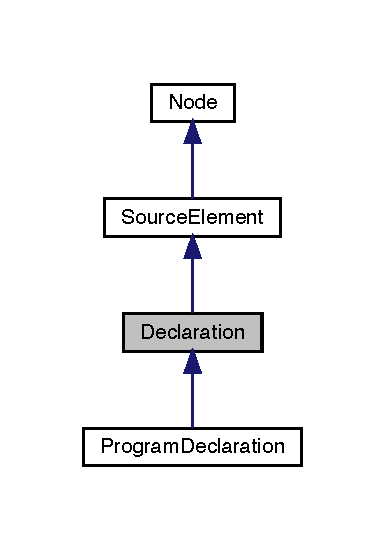
\includegraphics[width=185pt]{struct_declaration__inherit__graph}
\end{center}
\end{figure}


Collaboration diagram for Declaration\+:
\nopagebreak
\begin{figure}[H]
\begin{center}
\leavevmode
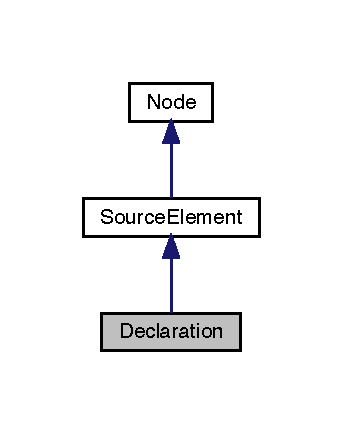
\includegraphics[width=164pt]{struct_declaration__coll__graph}
\end{center}
\end{figure}
\subsection*{Additional Inherited Members}


The documentation for this struct was generated from the following file\+:\begin{DoxyCompactItemize}
\item 
src/\hyperlink{ast_8h}{ast.\+h}\end{DoxyCompactItemize}

\hypertarget{struct_declarative_environment_record}{}\section{Declarative\+Environment\+Record Struct Reference}
\label{struct_declarative_environment_record}\index{Declarative\+Environment\+Record@{Declarative\+Environment\+Record}}


{\ttfamily \#include $<$declarative\+\_\+environment\+\_\+record.\+h$>$}



Inheritance diagram for Declarative\+Environment\+Record\+:
\nopagebreak
\begin{figure}[H]
\begin{center}
\leavevmode
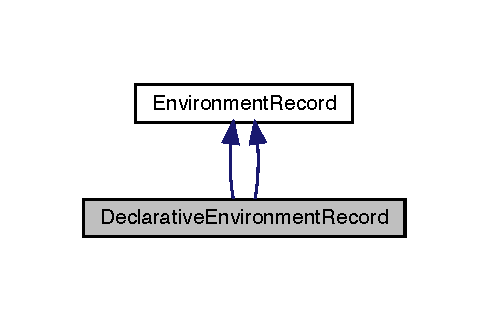
\includegraphics[width=234pt]{struct_declarative_environment_record__inherit__graph}
\end{center}
\end{figure}


Collaboration diagram for Declarative\+Environment\+Record\+:
\nopagebreak
\begin{figure}[H]
\begin{center}
\leavevmode
\includegraphics[width=234pt]{struct_declarative_environment_record__coll__graph}
\end{center}
\end{figure}
\subsection*{Public Member Functions}
\begin{DoxyCompactItemize}
\item 
bool \hyperlink{struct_declarative_environment_record_a4588f8af88b79f4317ced4dde8161813}{Has\+Binding} (const \textbf{ std\+::string} \&) final
\item 
void \hyperlink{struct_declarative_environment_record_aa2bc21d70c3869a2065e375dbadd5967}{Create\+Mutable\+Binding} (const \textbf{ std\+::string} \&, bool) final
\item 
void \hyperlink{struct_declarative_environment_record_a9e0b7b5b57e3125b4288a30e2ceac63c}{Set\+Mutable\+Binding} (const \textbf{ std\+::string} \&, const \hyperlink{class_type}{Type} \&, bool) final
\item 
\hyperlink{class_type}{Type} \hyperlink{struct_declarative_environment_record_a53765619db78e907bf5b0da354b2c7fc}{Get\+Binding\+Value} (const \textbf{ std\+::string} \&.bool) final
\item 
bool \hyperlink{struct_declarative_environment_record_ae21d2a351ca2b69110f11ffe13fd2380}{Delete\+Binding} (const \textbf{ std\+::string} \&) final
\item 
\hyperlink{class_type}{Type} \hyperlink{struct_declarative_environment_record_a0e5b27bb35773d4dbf994384265de1c8}{Implicit\+This\+Value} () final
\item 
void \hyperlink{struct_declarative_environment_record_a535362f458fd17e07740cfb066fff385}{Create\+Immutable\+Binding} (const \textbf{ std\+::string} \&)
\item 
void \hyperlink{struct_declarative_environment_record_afe3114f214e519ce7562e43adb5b54ae}{Initialize\+Immutable\+Binding} (const \textbf{ std\+::string} \&, const \hyperlink{class_type}{Type} \&)
\item 
\hyperlink{struct_boolean}{Boolean} \hyperlink{struct_declarative_environment_record_a76b1f7c3be69f63d9711e256b81738d5}{Has\+Binding} (const \hyperlink{struct_string}{String} \&N) const final
\item 
void \hyperlink{struct_declarative_environment_record_af71c0900f0d02f7a74cfd60b0655a9b5}{Create\+Mutable\+Binding} (const \hyperlink{struct_string}{String} \&N, const \hyperlink{struct_boolean}{Boolean} \&D) final
\item 
void \hyperlink{struct_declarative_environment_record_aa1136051a94789af3f2f4b75f0266a04}{Set\+Mutable\+Binding} (\hyperlink{struct_environment_record_ab67bd5dbacae338473147ec3f753a364}{String\+Ref}, const \hyperlink{class_type}{Type} \&, const \hyperlink{struct_boolean}{Boolean} \&) final
\item 
\hyperlink{class_type}{Type} \hyperlink{struct_declarative_environment_record_a886564d5370eb7b2b48a5616c4d1d33a}{Get\+Binding\+Value} (const \hyperlink{struct_string}{String} \&, const \hyperlink{struct_boolean}{Boolean} \&S) const final
\item 
\hyperlink{struct_boolean}{Boolean} \hyperlink{struct_declarative_environment_record_a853cee614241af5f32d9d3cb11d7e6d6}{Delete\+Binding} (const \hyperlink{struct_string}{String} \&) final
\item 
\hyperlink{class_type}{Type} \hyperlink{struct_declarative_environment_record_aafb5da7123366dd48562e07fd393af2d}{Implicit\+This\+Value} () const final
\item 
void \hyperlink{struct_declarative_environment_record_aeab8fc1f5c756454e5c036889b9609ef}{Create\+Immutable\+Binding} (const \hyperlink{struct_string}{String} \&)
\item 
void \hyperlink{struct_declarative_environment_record_ae2d908d84c12f6155dcb174a38bb7277}{Initialize\+Immutable\+Binding} (const \hyperlink{struct_string}{String} \&, const \hyperlink{class_type}{Type} \&)
\end{DoxyCompactItemize}
\subsection*{Additional Inherited Members}


\subsection{Member Function Documentation}
\mbox{\Hypertarget{struct_declarative_environment_record_a535362f458fd17e07740cfb066fff385}\label{struct_declarative_environment_record_a535362f458fd17e07740cfb066fff385}} 
\index{Declarative\+Environment\+Record@{Declarative\+Environment\+Record}!Create\+Immutable\+Binding@{Create\+Immutable\+Binding}}
\index{Create\+Immutable\+Binding@{Create\+Immutable\+Binding}!Declarative\+Environment\+Record@{Declarative\+Environment\+Record}}
\subsubsection{\texorpdfstring{Create\+Immutable\+Binding()}{CreateImmutableBinding()}\hspace{0.1cm}{\footnotesize\ttfamily [1/2]}}
{\footnotesize\ttfamily void Declarative\+Environment\+Record\+::\+Create\+Immutable\+Binding (\begin{DoxyParamCaption}\item[{const \textbf{ std\+::string} \&}]{ }\end{DoxyParamCaption})}

\mbox{\Hypertarget{struct_declarative_environment_record_aeab8fc1f5c756454e5c036889b9609ef}\label{struct_declarative_environment_record_aeab8fc1f5c756454e5c036889b9609ef}} 
\index{Declarative\+Environment\+Record@{Declarative\+Environment\+Record}!Create\+Immutable\+Binding@{Create\+Immutable\+Binding}}
\index{Create\+Immutable\+Binding@{Create\+Immutable\+Binding}!Declarative\+Environment\+Record@{Declarative\+Environment\+Record}}
\subsubsection{\texorpdfstring{Create\+Immutable\+Binding()}{CreateImmutableBinding()}\hspace{0.1cm}{\footnotesize\ttfamily [2/2]}}
{\footnotesize\ttfamily void Declarative\+Environment\+Record\+::\+Create\+Immutable\+Binding (\begin{DoxyParamCaption}\item[{const \hyperlink{struct_string}{String} \&}]{ }\end{DoxyParamCaption})}

\mbox{\Hypertarget{struct_declarative_environment_record_aa2bc21d70c3869a2065e375dbadd5967}\label{struct_declarative_environment_record_aa2bc21d70c3869a2065e375dbadd5967}} 
\index{Declarative\+Environment\+Record@{Declarative\+Environment\+Record}!Create\+Mutable\+Binding@{Create\+Mutable\+Binding}}
\index{Create\+Mutable\+Binding@{Create\+Mutable\+Binding}!Declarative\+Environment\+Record@{Declarative\+Environment\+Record}}
\subsubsection{\texorpdfstring{Create\+Mutable\+Binding()}{CreateMutableBinding()}\hspace{0.1cm}{\footnotesize\ttfamily [1/2]}}
{\footnotesize\ttfamily void Declarative\+Environment\+Record\+::\+Create\+Mutable\+Binding (\begin{DoxyParamCaption}\item[{const \textbf{ std\+::string} \&}]{,  }\item[{bool}]{ }\end{DoxyParamCaption})\hspace{0.3cm}{\ttfamily [final]}, {\ttfamily [virtual]}}



Implements \hyperlink{struct_environment_record_af5563437dc966f3ad9bbafe951375e23}{Environment\+Record}.

\mbox{\Hypertarget{struct_declarative_environment_record_af71c0900f0d02f7a74cfd60b0655a9b5}\label{struct_declarative_environment_record_af71c0900f0d02f7a74cfd60b0655a9b5}} 
\index{Declarative\+Environment\+Record@{Declarative\+Environment\+Record}!Create\+Mutable\+Binding@{Create\+Mutable\+Binding}}
\index{Create\+Mutable\+Binding@{Create\+Mutable\+Binding}!Declarative\+Environment\+Record@{Declarative\+Environment\+Record}}
\subsubsection{\texorpdfstring{Create\+Mutable\+Binding()}{CreateMutableBinding()}\hspace{0.1cm}{\footnotesize\ttfamily [2/2]}}
{\footnotesize\ttfamily void Declarative\+Environment\+Record\+::\+Create\+Mutable\+Binding (\begin{DoxyParamCaption}\item[{const \hyperlink{struct_string}{String} \&}]{N,  }\item[{const \hyperlink{struct_boolean}{Boolean} \&}]{D }\end{DoxyParamCaption})\hspace{0.3cm}{\ttfamily [final]}, {\ttfamily [virtual]}}



Implements \hyperlink{struct_environment_record_aded45e79485e73e080980e6ff611dc0d}{Environment\+Record}.

\mbox{\Hypertarget{struct_declarative_environment_record_ae21d2a351ca2b69110f11ffe13fd2380}\label{struct_declarative_environment_record_ae21d2a351ca2b69110f11ffe13fd2380}} 
\index{Declarative\+Environment\+Record@{Declarative\+Environment\+Record}!Delete\+Binding@{Delete\+Binding}}
\index{Delete\+Binding@{Delete\+Binding}!Declarative\+Environment\+Record@{Declarative\+Environment\+Record}}
\subsubsection{\texorpdfstring{Delete\+Binding()}{DeleteBinding()}\hspace{0.1cm}{\footnotesize\ttfamily [1/2]}}
{\footnotesize\ttfamily bool Declarative\+Environment\+Record\+::\+Delete\+Binding (\begin{DoxyParamCaption}\item[{const \textbf{ std\+::string} \&}]{ }\end{DoxyParamCaption})\hspace{0.3cm}{\ttfamily [final]}, {\ttfamily [virtual]}}



Implements \hyperlink{struct_environment_record_a41079a3969168b9fc4839fd89aa14dc0}{Environment\+Record}.

\mbox{\Hypertarget{struct_declarative_environment_record_a853cee614241af5f32d9d3cb11d7e6d6}\label{struct_declarative_environment_record_a853cee614241af5f32d9d3cb11d7e6d6}} 
\index{Declarative\+Environment\+Record@{Declarative\+Environment\+Record}!Delete\+Binding@{Delete\+Binding}}
\index{Delete\+Binding@{Delete\+Binding}!Declarative\+Environment\+Record@{Declarative\+Environment\+Record}}
\subsubsection{\texorpdfstring{Delete\+Binding()}{DeleteBinding()}\hspace{0.1cm}{\footnotesize\ttfamily [2/2]}}
{\footnotesize\ttfamily \hyperlink{struct_boolean}{Boolean} Declarative\+Environment\+Record\+::\+Delete\+Binding (\begin{DoxyParamCaption}\item[{const \hyperlink{struct_string}{String} \&}]{ }\end{DoxyParamCaption})\hspace{0.3cm}{\ttfamily [final]}, {\ttfamily [virtual]}}



Implements \hyperlink{struct_environment_record_ac8fe8ad8e0146d5d7e3d9c0f3d873717}{Environment\+Record}.

\mbox{\Hypertarget{struct_declarative_environment_record_a53765619db78e907bf5b0da354b2c7fc}\label{struct_declarative_environment_record_a53765619db78e907bf5b0da354b2c7fc}} 
\index{Declarative\+Environment\+Record@{Declarative\+Environment\+Record}!Get\+Binding\+Value@{Get\+Binding\+Value}}
\index{Get\+Binding\+Value@{Get\+Binding\+Value}!Declarative\+Environment\+Record@{Declarative\+Environment\+Record}}
\subsubsection{\texorpdfstring{Get\+Binding\+Value()}{GetBindingValue()}\hspace{0.1cm}{\footnotesize\ttfamily [1/2]}}
{\footnotesize\ttfamily \hyperlink{class_type}{Type} Declarative\+Environment\+Record\+::\+Get\+Binding\+Value (\begin{DoxyParamCaption}\item[{const \textbf{ std\+::string} \&.}]{bool }\end{DoxyParamCaption})\hspace{0.3cm}{\ttfamily [final]}, {\ttfamily [virtual]}}



Implements \hyperlink{struct_environment_record_afd78e04157f5d84cac025d2b0c867b4e}{Environment\+Record}.

\mbox{\Hypertarget{struct_declarative_environment_record_a886564d5370eb7b2b48a5616c4d1d33a}\label{struct_declarative_environment_record_a886564d5370eb7b2b48a5616c4d1d33a}} 
\index{Declarative\+Environment\+Record@{Declarative\+Environment\+Record}!Get\+Binding\+Value@{Get\+Binding\+Value}}
\index{Get\+Binding\+Value@{Get\+Binding\+Value}!Declarative\+Environment\+Record@{Declarative\+Environment\+Record}}
\subsubsection{\texorpdfstring{Get\+Binding\+Value()}{GetBindingValue()}\hspace{0.1cm}{\footnotesize\ttfamily [2/2]}}
{\footnotesize\ttfamily \hyperlink{class_type}{Type} Declarative\+Environment\+Record\+::\+Get\+Binding\+Value (\begin{DoxyParamCaption}\item[{const \hyperlink{struct_string}{String} \&}]{,  }\item[{const \hyperlink{struct_boolean}{Boolean} \&}]{S }\end{DoxyParamCaption}) const\hspace{0.3cm}{\ttfamily [final]}, {\ttfamily [virtual]}}



Implements \hyperlink{struct_environment_record_a38f1293eb4b23d22c0ee37ffff58dbdb}{Environment\+Record}.

\mbox{\Hypertarget{struct_declarative_environment_record_a4588f8af88b79f4317ced4dde8161813}\label{struct_declarative_environment_record_a4588f8af88b79f4317ced4dde8161813}} 
\index{Declarative\+Environment\+Record@{Declarative\+Environment\+Record}!Has\+Binding@{Has\+Binding}}
\index{Has\+Binding@{Has\+Binding}!Declarative\+Environment\+Record@{Declarative\+Environment\+Record}}
\subsubsection{\texorpdfstring{Has\+Binding()}{HasBinding()}\hspace{0.1cm}{\footnotesize\ttfamily [1/2]}}
{\footnotesize\ttfamily bool Declarative\+Environment\+Record\+::\+Has\+Binding (\begin{DoxyParamCaption}\item[{const \textbf{ std\+::string} \&}]{ }\end{DoxyParamCaption})\hspace{0.3cm}{\ttfamily [final]}, {\ttfamily [virtual]}}



Implements \hyperlink{struct_environment_record_aa9e241cd34f23e84ecaa19cf35657e9e}{Environment\+Record}.

\mbox{\Hypertarget{struct_declarative_environment_record_a76b1f7c3be69f63d9711e256b81738d5}\label{struct_declarative_environment_record_a76b1f7c3be69f63d9711e256b81738d5}} 
\index{Declarative\+Environment\+Record@{Declarative\+Environment\+Record}!Has\+Binding@{Has\+Binding}}
\index{Has\+Binding@{Has\+Binding}!Declarative\+Environment\+Record@{Declarative\+Environment\+Record}}
\subsubsection{\texorpdfstring{Has\+Binding()}{HasBinding()}\hspace{0.1cm}{\footnotesize\ttfamily [2/2]}}
{\footnotesize\ttfamily \hyperlink{struct_boolean}{Boolean} Declarative\+Environment\+Record\+::\+Has\+Binding (\begin{DoxyParamCaption}\item[{const \hyperlink{struct_string}{String} \&}]{N }\end{DoxyParamCaption}) const\hspace{0.3cm}{\ttfamily [final]}, {\ttfamily [virtual]}}



Implements \hyperlink{struct_environment_record_a4e9bc2438be3466fd0d9607cdbd20225}{Environment\+Record}.

\mbox{\Hypertarget{struct_declarative_environment_record_a0e5b27bb35773d4dbf994384265de1c8}\label{struct_declarative_environment_record_a0e5b27bb35773d4dbf994384265de1c8}} 
\index{Declarative\+Environment\+Record@{Declarative\+Environment\+Record}!Implicit\+This\+Value@{Implicit\+This\+Value}}
\index{Implicit\+This\+Value@{Implicit\+This\+Value}!Declarative\+Environment\+Record@{Declarative\+Environment\+Record}}
\subsubsection{\texorpdfstring{Implicit\+This\+Value()}{ImplicitThisValue()}\hspace{0.1cm}{\footnotesize\ttfamily [1/2]}}
{\footnotesize\ttfamily \hyperlink{class_type}{Type} Declarative\+Environment\+Record\+::\+Implicit\+This\+Value (\begin{DoxyParamCaption}{ }\end{DoxyParamCaption})\hspace{0.3cm}{\ttfamily [final]}, {\ttfamily [virtual]}}



Implements \hyperlink{struct_environment_record_acef5c0dac3d58cbef25daa495c5d0e00}{Environment\+Record}.

\mbox{\Hypertarget{struct_declarative_environment_record_aafb5da7123366dd48562e07fd393af2d}\label{struct_declarative_environment_record_aafb5da7123366dd48562e07fd393af2d}} 
\index{Declarative\+Environment\+Record@{Declarative\+Environment\+Record}!Implicit\+This\+Value@{Implicit\+This\+Value}}
\index{Implicit\+This\+Value@{Implicit\+This\+Value}!Declarative\+Environment\+Record@{Declarative\+Environment\+Record}}
\subsubsection{\texorpdfstring{Implicit\+This\+Value()}{ImplicitThisValue()}\hspace{0.1cm}{\footnotesize\ttfamily [2/2]}}
{\footnotesize\ttfamily \hyperlink{class_type}{Type} Declarative\+Environment\+Record\+::\+Implicit\+This\+Value (\begin{DoxyParamCaption}{ }\end{DoxyParamCaption}) const\hspace{0.3cm}{\ttfamily [final]}, {\ttfamily [virtual]}}



Implements \hyperlink{struct_environment_record_a9c60c0ab4900f6a8cdc50ceefdbf0507}{Environment\+Record}.

\mbox{\Hypertarget{struct_declarative_environment_record_afe3114f214e519ce7562e43adb5b54ae}\label{struct_declarative_environment_record_afe3114f214e519ce7562e43adb5b54ae}} 
\index{Declarative\+Environment\+Record@{Declarative\+Environment\+Record}!Initialize\+Immutable\+Binding@{Initialize\+Immutable\+Binding}}
\index{Initialize\+Immutable\+Binding@{Initialize\+Immutable\+Binding}!Declarative\+Environment\+Record@{Declarative\+Environment\+Record}}
\subsubsection{\texorpdfstring{Initialize\+Immutable\+Binding()}{InitializeImmutableBinding()}\hspace{0.1cm}{\footnotesize\ttfamily [1/2]}}
{\footnotesize\ttfamily void Declarative\+Environment\+Record\+::\+Initialize\+Immutable\+Binding (\begin{DoxyParamCaption}\item[{const \textbf{ std\+::string} \&}]{,  }\item[{const \hyperlink{class_type}{Type} \&}]{ }\end{DoxyParamCaption})}

\mbox{\Hypertarget{struct_declarative_environment_record_ae2d908d84c12f6155dcb174a38bb7277}\label{struct_declarative_environment_record_ae2d908d84c12f6155dcb174a38bb7277}} 
\index{Declarative\+Environment\+Record@{Declarative\+Environment\+Record}!Initialize\+Immutable\+Binding@{Initialize\+Immutable\+Binding}}
\index{Initialize\+Immutable\+Binding@{Initialize\+Immutable\+Binding}!Declarative\+Environment\+Record@{Declarative\+Environment\+Record}}
\subsubsection{\texorpdfstring{Initialize\+Immutable\+Binding()}{InitializeImmutableBinding()}\hspace{0.1cm}{\footnotesize\ttfamily [2/2]}}
{\footnotesize\ttfamily void Declarative\+Environment\+Record\+::\+Initialize\+Immutable\+Binding (\begin{DoxyParamCaption}\item[{const \hyperlink{struct_string}{String} \&}]{,  }\item[{const \hyperlink{class_type}{Type} \&}]{ }\end{DoxyParamCaption})}

\mbox{\Hypertarget{struct_declarative_environment_record_a9e0b7b5b57e3125b4288a30e2ceac63c}\label{struct_declarative_environment_record_a9e0b7b5b57e3125b4288a30e2ceac63c}} 
\index{Declarative\+Environment\+Record@{Declarative\+Environment\+Record}!Set\+Mutable\+Binding@{Set\+Mutable\+Binding}}
\index{Set\+Mutable\+Binding@{Set\+Mutable\+Binding}!Declarative\+Environment\+Record@{Declarative\+Environment\+Record}}
\subsubsection{\texorpdfstring{Set\+Mutable\+Binding()}{SetMutableBinding()}\hspace{0.1cm}{\footnotesize\ttfamily [1/2]}}
{\footnotesize\ttfamily void Declarative\+Environment\+Record\+::\+Set\+Mutable\+Binding (\begin{DoxyParamCaption}\item[{const \textbf{ std\+::string} \&}]{,  }\item[{const \hyperlink{class_type}{Type} \&}]{,  }\item[{bool}]{ }\end{DoxyParamCaption})\hspace{0.3cm}{\ttfamily [final]}, {\ttfamily [virtual]}}



Implements \hyperlink{struct_environment_record_a9d5250a9cc6fa4d1f9ecbf5213b6cb24}{Environment\+Record}.

\mbox{\Hypertarget{struct_declarative_environment_record_aa1136051a94789af3f2f4b75f0266a04}\label{struct_declarative_environment_record_aa1136051a94789af3f2f4b75f0266a04}} 
\index{Declarative\+Environment\+Record@{Declarative\+Environment\+Record}!Set\+Mutable\+Binding@{Set\+Mutable\+Binding}}
\index{Set\+Mutable\+Binding@{Set\+Mutable\+Binding}!Declarative\+Environment\+Record@{Declarative\+Environment\+Record}}
\subsubsection{\texorpdfstring{Set\+Mutable\+Binding()}{SetMutableBinding()}\hspace{0.1cm}{\footnotesize\ttfamily [2/2]}}
{\footnotesize\ttfamily void Declarative\+Environment\+Record\+::\+Set\+Mutable\+Binding (\begin{DoxyParamCaption}\item[{\hyperlink{struct_environment_record_ab67bd5dbacae338473147ec3f753a364}{String\+Ref}}]{,  }\item[{const \hyperlink{class_type}{Type} \&}]{,  }\item[{const \hyperlink{struct_boolean}{Boolean} \&}]{ }\end{DoxyParamCaption})\hspace{0.3cm}{\ttfamily [final]}, {\ttfamily [virtual]}}



Implements \hyperlink{struct_environment_record_ae5268e78f690c5f9eb50d8abe2342fff}{Environment\+Record}.



The documentation for this struct was generated from the following files\+:\begin{DoxyCompactItemize}
\item 
src/\hyperlink{declarative__environment__record_8h}{declarative\+\_\+environment\+\_\+record.\+h}\item 
src/\hyperlink{runtime_8h}{runtime.\+h}\end{DoxyCompactItemize}

\hypertarget{struct_catch_1_1_decomposed_expression}{}\section{Catch\+:\+:Decomposed\+Expression Struct Reference}
\label{struct_catch_1_1_decomposed_expression}\index{Catch\+::\+Decomposed\+Expression@{Catch\+::\+Decomposed\+Expression}}


{\ttfamily \#include $<$catch.\+hpp$>$}



Inheritance diagram for Catch\+:\+:Decomposed\+Expression\+:
\nopagebreak
\begin{figure}[H]
\begin{center}
\leavevmode
\includegraphics[width=350pt]{struct_catch_1_1_decomposed_expression__inherit__graph}
\end{center}
\end{figure}
\subsection*{Public Member Functions}
\begin{DoxyCompactItemize}
\item 
virtual \hyperlink{struct_catch_1_1_decomposed_expression_aa627c69bd83582c33a4d4dcac403936c}{$\sim$\+Decomposed\+Expression} ()
\item 
virtual bool \hyperlink{struct_catch_1_1_decomposed_expression_a1c458ece47b71f093290dbdf9bb31fdb}{is\+Binary\+Expression} () const
\item 
virtual void \hyperlink{struct_catch_1_1_decomposed_expression_a9ce7f356dc96f11f80e40c82f5aa7e55}{reconstruct\+Expression} (\textbf{ std\+::string} \&dest) const =0
\item 
{\footnotesize template$<$typename T $>$ }\\S\+T\+A\+T\+I\+C\+\_\+\+A\+S\+S\+E\+R\+T\+\_\+\+Expression\+\_\+\+Too\+\_\+\+Complex\+\_\+\+Please\+\_\+\+Rewrite\+\_\+\+As\+\_\+\+Binary\+\_\+\+Comparison \& \hyperlink{struct_catch_1_1_decomposed_expression_aa2ce96ce31fef4afb21861bc0276edb9}{operator+} (T const \&)
\item 
{\footnotesize template$<$typename T $>$ }\\S\+T\+A\+T\+I\+C\+\_\+\+A\+S\+S\+E\+R\+T\+\_\+\+Expression\+\_\+\+Too\+\_\+\+Complex\+\_\+\+Please\+\_\+\+Rewrite\+\_\+\+As\+\_\+\+Binary\+\_\+\+Comparison \& \hyperlink{struct_catch_1_1_decomposed_expression_aff39fb5d060abbd018c83b998d32c366}{operator-\/} (T const \&)
\item 
{\footnotesize template$<$typename T $>$ }\\S\+T\+A\+T\+I\+C\+\_\+\+A\+S\+S\+E\+R\+T\+\_\+\+Expression\+\_\+\+Too\+\_\+\+Complex\+\_\+\+Please\+\_\+\+Rewrite\+\_\+\+As\+\_\+\+Binary\+\_\+\+Comparison \& \hyperlink{struct_catch_1_1_decomposed_expression_afb5527e8e3cb8edca5113ec9801249d8}{operator$\ast$} (T const \&)
\item 
{\footnotesize template$<$typename T $>$ }\\S\+T\+A\+T\+I\+C\+\_\+\+A\+S\+S\+E\+R\+T\+\_\+\+Expression\+\_\+\+Too\+\_\+\+Complex\+\_\+\+Please\+\_\+\+Rewrite\+\_\+\+As\+\_\+\+Binary\+\_\+\+Comparison \& \hyperlink{struct_catch_1_1_decomposed_expression_a519d7e2363a92106e46371c9c04044a7}{operator/} (T const \&)
\item 
{\footnotesize template$<$typename T $>$ }\\S\+T\+A\+T\+I\+C\+\_\+\+A\+S\+S\+E\+R\+T\+\_\+\+Expression\+\_\+\+Too\+\_\+\+Complex\+\_\+\+Please\+\_\+\+Rewrite\+\_\+\+As\+\_\+\+Binary\+\_\+\+Comparison \& \hyperlink{struct_catch_1_1_decomposed_expression_a6584335aadaee847c9d06ca8f13a4477}{operator\%} (T const \&)
\item 
{\footnotesize template$<$typename T $>$ }\\S\+T\+A\+T\+I\+C\+\_\+\+A\+S\+S\+E\+R\+T\+\_\+\+Expression\+\_\+\+Too\+\_\+\+Complex\+\_\+\+Please\+\_\+\+Rewrite\+\_\+\+As\+\_\+\+Binary\+\_\+\+Comparison \& \hyperlink{struct_catch_1_1_decomposed_expression_a14d913535796145b39101a16c0c490da}{operator\&\&} (T const \&)
\item 
{\footnotesize template$<$typename T $>$ }\\S\+T\+A\+T\+I\+C\+\_\+\+A\+S\+S\+E\+R\+T\+\_\+\+Expression\+\_\+\+Too\+\_\+\+Complex\+\_\+\+Please\+\_\+\+Rewrite\+\_\+\+As\+\_\+\+Binary\+\_\+\+Comparison \& \hyperlink{struct_catch_1_1_decomposed_expression_ab4800d277290088fea9c594cfdd4f1c7}{operator$\vert$$\vert$} (T const \&)
\end{DoxyCompactItemize}


\subsection{Constructor \& Destructor Documentation}
\mbox{\Hypertarget{struct_catch_1_1_decomposed_expression_aa627c69bd83582c33a4d4dcac403936c}\label{struct_catch_1_1_decomposed_expression_aa627c69bd83582c33a4d4dcac403936c}} 
\index{Catch\+::\+Decomposed\+Expression@{Catch\+::\+Decomposed\+Expression}!````~Decomposed\+Expression@{$\sim$\+Decomposed\+Expression}}
\index{````~Decomposed\+Expression@{$\sim$\+Decomposed\+Expression}!Catch\+::\+Decomposed\+Expression@{Catch\+::\+Decomposed\+Expression}}
\subsubsection{\texorpdfstring{$\sim$\+Decomposed\+Expression()}{~DecomposedExpression()}}
{\footnotesize\ttfamily virtual Catch\+::\+Decomposed\+Expression\+::$\sim$\+Decomposed\+Expression (\begin{DoxyParamCaption}{ }\end{DoxyParamCaption})\hspace{0.3cm}{\ttfamily [inline]}, {\ttfamily [virtual]}}



\subsection{Member Function Documentation}
\mbox{\Hypertarget{struct_catch_1_1_decomposed_expression_a1c458ece47b71f093290dbdf9bb31fdb}\label{struct_catch_1_1_decomposed_expression_a1c458ece47b71f093290dbdf9bb31fdb}} 
\index{Catch\+::\+Decomposed\+Expression@{Catch\+::\+Decomposed\+Expression}!is\+Binary\+Expression@{is\+Binary\+Expression}}
\index{is\+Binary\+Expression@{is\+Binary\+Expression}!Catch\+::\+Decomposed\+Expression@{Catch\+::\+Decomposed\+Expression}}
\subsubsection{\texorpdfstring{is\+Binary\+Expression()}{isBinaryExpression()}}
{\footnotesize\ttfamily virtual bool Catch\+::\+Decomposed\+Expression\+::is\+Binary\+Expression (\begin{DoxyParamCaption}{ }\end{DoxyParamCaption}) const\hspace{0.3cm}{\ttfamily [inline]}, {\ttfamily [virtual]}}



Reimplemented in \hyperlink{class_catch_1_1_match_expression_ac4edf6e9a6e5762a487db1486d0d1f45}{Catch\+::\+Match\+Expression$<$ Arg\+T, Matcher\+T $>$}, and \hyperlink{class_catch_1_1_binary_expression_a4c617c0b6a73a9cafbbf900909c7c258}{Catch\+::\+Binary\+Expression$<$ Lhs\+T, Op, Rhs\+T $>$}.

\mbox{\Hypertarget{struct_catch_1_1_decomposed_expression_a6584335aadaee847c9d06ca8f13a4477}\label{struct_catch_1_1_decomposed_expression_a6584335aadaee847c9d06ca8f13a4477}} 
\index{Catch\+::\+Decomposed\+Expression@{Catch\+::\+Decomposed\+Expression}!operator\%@{operator\%}}
\index{operator\%@{operator\%}!Catch\+::\+Decomposed\+Expression@{Catch\+::\+Decomposed\+Expression}}
\subsubsection{\texorpdfstring{operator\%()}{operator\%()}}
{\footnotesize\ttfamily template$<$typename T $>$ \\
S\+T\+A\+T\+I\+C\+\_\+\+A\+S\+S\+E\+R\+T\+\_\+\+Expression\+\_\+\+Too\+\_\+\+Complex\+\_\+\+Please\+\_\+\+Rewrite\+\_\+\+As\+\_\+\+Binary\+\_\+\+Comparison\& Catch\+::\+Decomposed\+Expression\+::operator\% (\begin{DoxyParamCaption}\item[{T const \&}]{ }\end{DoxyParamCaption})}

\mbox{\Hypertarget{struct_catch_1_1_decomposed_expression_a14d913535796145b39101a16c0c490da}\label{struct_catch_1_1_decomposed_expression_a14d913535796145b39101a16c0c490da}} 
\index{Catch\+::\+Decomposed\+Expression@{Catch\+::\+Decomposed\+Expression}!operator\&\&@{operator\&\&}}
\index{operator\&\&@{operator\&\&}!Catch\+::\+Decomposed\+Expression@{Catch\+::\+Decomposed\+Expression}}
\subsubsection{\texorpdfstring{operator\&\&()}{operator\&\&()}}
{\footnotesize\ttfamily template$<$typename T $>$ \\
S\+T\+A\+T\+I\+C\+\_\+\+A\+S\+S\+E\+R\+T\+\_\+\+Expression\+\_\+\+Too\+\_\+\+Complex\+\_\+\+Please\+\_\+\+Rewrite\+\_\+\+As\+\_\+\+Binary\+\_\+\+Comparison\& Catch\+::\+Decomposed\+Expression\+::operator \&\& (\begin{DoxyParamCaption}\item[{T const \&}]{ }\end{DoxyParamCaption})}

\mbox{\Hypertarget{struct_catch_1_1_decomposed_expression_afb5527e8e3cb8edca5113ec9801249d8}\label{struct_catch_1_1_decomposed_expression_afb5527e8e3cb8edca5113ec9801249d8}} 
\index{Catch\+::\+Decomposed\+Expression@{Catch\+::\+Decomposed\+Expression}!operator$\ast$@{operator$\ast$}}
\index{operator$\ast$@{operator$\ast$}!Catch\+::\+Decomposed\+Expression@{Catch\+::\+Decomposed\+Expression}}
\subsubsection{\texorpdfstring{operator$\ast$()}{operator*()}}
{\footnotesize\ttfamily template$<$typename T $>$ \\
S\+T\+A\+T\+I\+C\+\_\+\+A\+S\+S\+E\+R\+T\+\_\+\+Expression\+\_\+\+Too\+\_\+\+Complex\+\_\+\+Please\+\_\+\+Rewrite\+\_\+\+As\+\_\+\+Binary\+\_\+\+Comparison\& Catch\+::\+Decomposed\+Expression\+::operator$\ast$ (\begin{DoxyParamCaption}\item[{T const \&}]{ }\end{DoxyParamCaption})}

\mbox{\Hypertarget{struct_catch_1_1_decomposed_expression_aa2ce96ce31fef4afb21861bc0276edb9}\label{struct_catch_1_1_decomposed_expression_aa2ce96ce31fef4afb21861bc0276edb9}} 
\index{Catch\+::\+Decomposed\+Expression@{Catch\+::\+Decomposed\+Expression}!operator+@{operator+}}
\index{operator+@{operator+}!Catch\+::\+Decomposed\+Expression@{Catch\+::\+Decomposed\+Expression}}
\subsubsection{\texorpdfstring{operator+()}{operator+()}}
{\footnotesize\ttfamily template$<$typename T $>$ \\
S\+T\+A\+T\+I\+C\+\_\+\+A\+S\+S\+E\+R\+T\+\_\+\+Expression\+\_\+\+Too\+\_\+\+Complex\+\_\+\+Please\+\_\+\+Rewrite\+\_\+\+As\+\_\+\+Binary\+\_\+\+Comparison\& Catch\+::\+Decomposed\+Expression\+::operator+ (\begin{DoxyParamCaption}\item[{T const \&}]{ }\end{DoxyParamCaption})}

\mbox{\Hypertarget{struct_catch_1_1_decomposed_expression_aff39fb5d060abbd018c83b998d32c366}\label{struct_catch_1_1_decomposed_expression_aff39fb5d060abbd018c83b998d32c366}} 
\index{Catch\+::\+Decomposed\+Expression@{Catch\+::\+Decomposed\+Expression}!operator-\/@{operator-\/}}
\index{operator-\/@{operator-\/}!Catch\+::\+Decomposed\+Expression@{Catch\+::\+Decomposed\+Expression}}
\subsubsection{\texorpdfstring{operator-\/()}{operator-()}}
{\footnotesize\ttfamily template$<$typename T $>$ \\
S\+T\+A\+T\+I\+C\+\_\+\+A\+S\+S\+E\+R\+T\+\_\+\+Expression\+\_\+\+Too\+\_\+\+Complex\+\_\+\+Please\+\_\+\+Rewrite\+\_\+\+As\+\_\+\+Binary\+\_\+\+Comparison\& Catch\+::\+Decomposed\+Expression\+::operator-\/ (\begin{DoxyParamCaption}\item[{T const \&}]{ }\end{DoxyParamCaption})}

\mbox{\Hypertarget{struct_catch_1_1_decomposed_expression_a519d7e2363a92106e46371c9c04044a7}\label{struct_catch_1_1_decomposed_expression_a519d7e2363a92106e46371c9c04044a7}} 
\index{Catch\+::\+Decomposed\+Expression@{Catch\+::\+Decomposed\+Expression}!operator/@{operator/}}
\index{operator/@{operator/}!Catch\+::\+Decomposed\+Expression@{Catch\+::\+Decomposed\+Expression}}
\subsubsection{\texorpdfstring{operator/()}{operator/()}}
{\footnotesize\ttfamily template$<$typename T $>$ \\
S\+T\+A\+T\+I\+C\+\_\+\+A\+S\+S\+E\+R\+T\+\_\+\+Expression\+\_\+\+Too\+\_\+\+Complex\+\_\+\+Please\+\_\+\+Rewrite\+\_\+\+As\+\_\+\+Binary\+\_\+\+Comparison\& Catch\+::\+Decomposed\+Expression\+::operator/ (\begin{DoxyParamCaption}\item[{T const \&}]{ }\end{DoxyParamCaption})}

\mbox{\Hypertarget{struct_catch_1_1_decomposed_expression_ab4800d277290088fea9c594cfdd4f1c7}\label{struct_catch_1_1_decomposed_expression_ab4800d277290088fea9c594cfdd4f1c7}} 
\index{Catch\+::\+Decomposed\+Expression@{Catch\+::\+Decomposed\+Expression}!operator\texttt{"|}\texttt{"|}@{operator\texttt{"|}\texttt{"|}}}
\index{operator\texttt{"|}\texttt{"|}@{operator\texttt{"|}\texttt{"|}}!Catch\+::\+Decomposed\+Expression@{Catch\+::\+Decomposed\+Expression}}
\subsubsection{\texorpdfstring{operator\texttt{"|}\texttt{"|}()}{operator||()}}
{\footnotesize\ttfamily template$<$typename T $>$ \\
S\+T\+A\+T\+I\+C\+\_\+\+A\+S\+S\+E\+R\+T\+\_\+\+Expression\+\_\+\+Too\+\_\+\+Complex\+\_\+\+Please\+\_\+\+Rewrite\+\_\+\+As\+\_\+\+Binary\+\_\+\+Comparison\& Catch\+::\+Decomposed\+Expression\+::operator$\vert$$\vert$ (\begin{DoxyParamCaption}\item[{T const \&}]{ }\end{DoxyParamCaption})}

\mbox{\Hypertarget{struct_catch_1_1_decomposed_expression_a9ce7f356dc96f11f80e40c82f5aa7e55}\label{struct_catch_1_1_decomposed_expression_a9ce7f356dc96f11f80e40c82f5aa7e55}} 
\index{Catch\+::\+Decomposed\+Expression@{Catch\+::\+Decomposed\+Expression}!reconstruct\+Expression@{reconstruct\+Expression}}
\index{reconstruct\+Expression@{reconstruct\+Expression}!Catch\+::\+Decomposed\+Expression@{Catch\+::\+Decomposed\+Expression}}
\subsubsection{\texorpdfstring{reconstruct\+Expression()}{reconstructExpression()}}
{\footnotesize\ttfamily virtual void Catch\+::\+Decomposed\+Expression\+::reconstruct\+Expression (\begin{DoxyParamCaption}\item[{\textbf{ std\+::string} \&}]{dest }\end{DoxyParamCaption}) const\hspace{0.3cm}{\ttfamily [pure virtual]}}



Implemented in \hyperlink{class_catch_1_1_match_expression_a4410a93bc5b8241eb2502f400fce7ec4}{Catch\+::\+Match\+Expression$<$ Arg\+T, Matcher\+T $>$}, \hyperlink{class_catch_1_1_binary_expression_a6ed73ff9af9c229f9fa3d35d019f9e37}{Catch\+::\+Binary\+Expression$<$ Lhs\+T, Op, Rhs\+T $>$}, \hyperlink{class_catch_1_1_expression_lhs_a7684a053e8e88a4be475a536252630da}{Catch\+::\+Expression\+Lhs$<$ T $>$}, and \hyperlink{class_catch_1_1_result_builder_a7d94b15cf04301a8617e7b16158b5d82}{Catch\+::\+Result\+Builder}.



The documentation for this struct was generated from the following file\+:\begin{DoxyCompactItemize}
\item 
src/\hyperlink{catch_8hpp}{catch.\+hpp}\end{DoxyCompactItemize}

\hypertarget{struct_default_clause}{}\section{Default\+Clause Struct Reference}
\label{struct_default_clause}\index{Default\+Clause@{Default\+Clause}}


{\ttfamily \#include $<$ast.\+h$>$}



Inheritance diagram for Default\+Clause\+:\nopagebreak
\begin{figure}[H]
\begin{center}
\leavevmode
\includegraphics[width=159pt]{struct_default_clause__inherit__graph}
\end{center}
\end{figure}


Collaboration diagram for Default\+Clause\+:\nopagebreak
\begin{figure}[H]
\begin{center}
\leavevmode
\includegraphics[width=268pt]{struct_default_clause__coll__graph}
\end{center}
\end{figure}
\subsection*{Public Member Functions}
\begin{DoxyCompactItemize}
\item 
\hyperlink{struct_default_clause_a9f15e6fc45dc6e8a3d87a02aa4798b25}{Default\+Clause} (\hyperlink{struct_statement_list}{Statement\+List} $\ast$\hyperlink{struct_case_clause_a3e6914411610d1893b61172521e11288}{consequent})
\item 
void \hyperlink{struct_default_clause_ade62e79cf9ad891d974528e1e172e2b6}{accept} (\hyperlink{struct_visitor}{Visitor} \&visitor) const override
\item 
const char $\ast$ \hyperlink{struct_default_clause_a464358dcd7e4e13287482d3c858f3538}{type} () const override
\end{DoxyCompactItemize}
\subsection*{Additional Inherited Members}


\subsection{Constructor \& Destructor Documentation}
\mbox{\Hypertarget{struct_default_clause_a9f15e6fc45dc6e8a3d87a02aa4798b25}\label{struct_default_clause_a9f15e6fc45dc6e8a3d87a02aa4798b25}} 
\index{Default\+Clause@{Default\+Clause}!Default\+Clause@{Default\+Clause}}
\index{Default\+Clause@{Default\+Clause}!Default\+Clause@{Default\+Clause}}
\subsubsection{\texorpdfstring{Default\+Clause()}{DefaultClause()}}
{\footnotesize\ttfamily Default\+Clause\+::\+Default\+Clause (\begin{DoxyParamCaption}\item[{\hyperlink{struct_statement_list}{Statement\+List} $\ast$}]{consequent }\end{DoxyParamCaption})\hspace{0.3cm}{\ttfamily [inline]}}



\subsection{Member Function Documentation}
\mbox{\Hypertarget{struct_default_clause_ade62e79cf9ad891d974528e1e172e2b6}\label{struct_default_clause_ade62e79cf9ad891d974528e1e172e2b6}} 
\index{Default\+Clause@{Default\+Clause}!accept@{accept}}
\index{accept@{accept}!Default\+Clause@{Default\+Clause}}
\subsubsection{\texorpdfstring{accept()}{accept()}}
{\footnotesize\ttfamily void Default\+Clause\+::accept (\begin{DoxyParamCaption}\item[{\hyperlink{struct_visitor}{Visitor} \&}]{visitor }\end{DoxyParamCaption}) const\hspace{0.3cm}{\ttfamily [inline]}, {\ttfamily [override]}, {\ttfamily [virtual]}}



Reimplemented from \hyperlink{struct_case_clause_a5bbee9ea9ca206c09b8b79f8c96720a1}{Case\+Clause}.

\mbox{\Hypertarget{struct_default_clause_a464358dcd7e4e13287482d3c858f3538}\label{struct_default_clause_a464358dcd7e4e13287482d3c858f3538}} 
\index{Default\+Clause@{Default\+Clause}!type@{type}}
\index{type@{type}!Default\+Clause@{Default\+Clause}}
\subsubsection{\texorpdfstring{type()}{type()}}
{\footnotesize\ttfamily const char$\ast$ Default\+Clause\+::type (\begin{DoxyParamCaption}{ }\end{DoxyParamCaption}) const\hspace{0.3cm}{\ttfamily [inline]}, {\ttfamily [override]}, {\ttfamily [virtual]}}



Reimplemented from \hyperlink{struct_case_clause_a9dcb0a1a072df7d577b272c6bbb3c6dc}{Case\+Clause}.



The documentation for this struct was generated from the following file\+:\begin{DoxyCompactItemize}
\item 
src/\hyperlink{ast_8h}{ast.\+h}\end{DoxyCompactItemize}

\hypertarget{struct_delegate_vistor}{}\section{Delegate\+Vistor Struct Reference}
\label{struct_delegate_vistor}\index{Delegate\+Vistor@{Delegate\+Vistor}}


Inheritance diagram for Delegate\+Vistor\+:
\nopagebreak
\begin{figure}[H]
\begin{center}
\leavevmode
\includegraphics[width=161pt]{struct_delegate_vistor__inherit__graph}
\end{center}
\end{figure}


Collaboration diagram for Delegate\+Vistor\+:
\nopagebreak
\begin{figure}[H]
\begin{center}
\leavevmode
\includegraphics[width=268pt]{struct_delegate_vistor__coll__graph}
\end{center}
\end{figure}
\subsection*{Public Member Functions}
\begin{DoxyCompactItemize}
\item 
{\footnotesize template$<$typename T $>$ }\\void \hyperlink{struct_delegate_vistor_af9662a5d46b463eaf5687383d0720da9}{invoke} (const T \&node)
\item 
void \hyperlink{struct_delegate_vistor_a8dace5cc6d8f07fa159bf17c0e2ab35d}{operator()} (const \hyperlink{struct_this}{This} \&node)
\item 
void \hyperlink{struct_delegate_vistor_ac0c8ef853f15168a8ecae04d0a901042}{operator()} (const \hyperlink{struct_identifier}{Identifier} \&node)
\item 
void \hyperlink{struct_delegate_vistor_aec595975fc76a47a9181b28cb1b07d28}{operator()} (const \hyperlink{struct_null_literal}{Null\+Literal} \&node)
\item 
void \hyperlink{struct_delegate_vistor_a5b0414c4f00fd368ce65ae03f44ad5a0}{operator()} (const \hyperlink{struct_boolean_literal}{Boolean\+Literal} \&node)
\item 
void \hyperlink{struct_delegate_vistor_a7447ce0cf89a2cce50016f1e6be2e427}{operator()} (const \hyperlink{struct_numeric_literal}{Numeric\+Literal} \&node)
\item 
void \hyperlink{struct_delegate_vistor_a8197fd5f76ca1c4c23de591522865081}{operator()} (const \hyperlink{struct_string_literal}{String\+Literal} \&node)
\item 
void \hyperlink{struct_delegate_vistor_a4850452c1da6f05c0bcae9797f6feec6}{operator()} (const \hyperlink{struct_regular_expression_literal}{Regular\+Expression\+Literal} \&node)
\item 
void \hyperlink{struct_delegate_vistor_a63960604451464f12d814c503025c04e}{operator()} (const \hyperlink{struct_array_literal}{Array\+Literal} \&node)
\item 
void \hyperlink{struct_delegate_vistor_a1f7ce208dd82aa1a7a13b605c8f15e42}{operator()} (const \hyperlink{struct_object_literal}{Object\+Literal} \&node)
\item 
void \hyperlink{struct_delegate_vistor_a04309f21f46080e60d5d9c2dc8d859ba}{operator()} (const \hyperlink{struct_this_expression}{This\+Expression} \&node)
\item 
void \hyperlink{struct_delegate_vistor_adfdd4d12c4212dc1e951f5fd915ff785}{operator()} (const \hyperlink{struct_identifier_expression}{Identifier\+Expression} \&node)
\item 
void \hyperlink{struct_delegate_vistor_aad5462e1d6053a95685e9807cc806093}{operator()} (const \hyperlink{struct_literal_expression}{Literal\+Expression} \&node)
\item 
void \hyperlink{struct_delegate_vistor_a1cd7a74dedbded5bba41928b218bbb48}{operator()} (const \hyperlink{struct_array_expression}{Array\+Expression} \&node)
\item 
void \hyperlink{struct_delegate_vistor_aae93fa71457dfb3c00d2249468f525b7}{operator()} (const \hyperlink{struct_object_expression}{Object\+Expression} \&node)
\item 
void \hyperlink{struct_delegate_vistor_a06f7d91b5f3472c286675d6490d00069}{operator()} (const \hyperlink{struct_member_expression}{Member\+Expression} \&node)
\item 
void \hyperlink{struct_delegate_vistor_a9b1c9874077d8bd184c8351a53e49af6}{operator()} (const \hyperlink{struct_new_expression}{New\+Expression} \&node)
\item 
void \hyperlink{struct_delegate_vistor_a1fc41883640efac8064e68c29850969c}{operator()} (const \hyperlink{struct_call_expression}{Call\+Expression} \&node)
\item 
void \hyperlink{struct_delegate_vistor_a8809fdcff726a6063e89bd96467e5f54}{operator()} (const \hyperlink{struct_postfix_expression}{Postfix\+Expression} \&node)
\item 
void \hyperlink{struct_delegate_vistor_a0fcc8b392984adc1a96ecebc7073383b}{operator()} (const \hyperlink{struct_unary_expression}{Unary\+Expression} \&node)
\item 
void \hyperlink{struct_delegate_vistor_a29aa74682b64ffb3fbaa487ac82eb370}{operator()} (const \hyperlink{struct_binary_expression}{Binary\+Expression} \&node)
\item 
void \hyperlink{struct_delegate_vistor_aaa62c8813386fe12d9ee8ce9705e4fa7}{operator()} (const \hyperlink{struct_conditional_expression}{Conditional\+Expression} \&node)
\item 
void \hyperlink{struct_delegate_vistor_a10977cba1c3e36b3096fac46d128b368}{operator()} (const \hyperlink{struct_assignment_expression}{Assignment\+Expression} \&node)
\item 
void \hyperlink{struct_delegate_vistor_a571b86616a181a82291d04fba7712faa}{operator()} (const \hyperlink{struct_function_expression}{Function\+Expression} \&node)
\item 
void \hyperlink{struct_delegate_vistor_a6a7679e5f0793edd951823764d518031}{operator()} (const \hyperlink{struct_block}{Block} \&node)
\item 
void \hyperlink{struct_delegate_vistor_acedb866730fb2a6935ce83fcca70e0f1}{operator()} (const \hyperlink{struct_variable_statement}{Variable\+Statement} \&node)
\item 
void \hyperlink{struct_delegate_vistor_aadd695f67dd5929c3685994bec2296e2}{operator()} (const \hyperlink{struct_empty_statement}{Empty\+Statement} \&node)
\item 
void \hyperlink{struct_delegate_vistor_af45b11b7a3b3bb2e213c182cd98c517e}{operator()} (const \hyperlink{struct_expression_statement}{Expression\+Statement} \&node)
\item 
void \hyperlink{struct_delegate_vistor_ab863b34aedf8480973ed8615a148da5d}{operator()} (const \hyperlink{struct_if_statement}{If\+Statement} \&node)
\item 
void \hyperlink{struct_delegate_vistor_ac997e241943d6fc8d8984824eb4026ba}{operator()} (const \hyperlink{struct_do_while_statement}{Do\+While\+Statement} \&node)
\item 
void \hyperlink{struct_delegate_vistor_a19f6de63901518dd85896e84f33121b1}{operator()} (const \hyperlink{struct_while_statement}{While\+Statement} \&node)
\item 
void \hyperlink{struct_delegate_vistor_a8b4de7ebaa6256d46fa35458a905b573}{operator()} (const \hyperlink{struct_for_statement}{For\+Statement} \&node)
\item 
void \hyperlink{struct_delegate_vistor_a5e977f00098da416b2ba8cce9e6815da}{operator()} (const \hyperlink{struct_for_in_statement}{For\+In\+Statement} \&node)
\item 
void \hyperlink{struct_delegate_vistor_a7e9c7e2831d4d1fd618fd5c2a4eed85e}{operator()} (const \hyperlink{struct_continue_statement}{Continue\+Statement} \&node)
\item 
void \hyperlink{struct_delegate_vistor_a6c4e9c57c90d0f19cc72307670798cb6}{operator()} (const \hyperlink{struct_break_statement}{Break\+Statement} \&node)
\item 
void \hyperlink{struct_delegate_vistor_a6b49bd2929b053a5b5eae78017c2bef6}{operator()} (const \hyperlink{struct_return_statement}{Return\+Statement} \&node)
\item 
void \hyperlink{struct_delegate_vistor_acc7c7102de95484e447db60c571e7178}{operator()} (const \hyperlink{struct_with_statement}{With\+Statement} \&node)
\item 
void \hyperlink{struct_delegate_vistor_a949fb1eb908425e833f83f43717e41dc}{operator()} (const \hyperlink{struct_labelled_statement}{Labelled\+Statement} \&node)
\item 
void \hyperlink{struct_delegate_vistor_ad35c29053e1e55df4fdfec753e2af65c}{operator()} (const \hyperlink{struct_switch_statement}{Switch\+Statement} \&node)
\item 
void \hyperlink{struct_delegate_vistor_ad63c1d6ae6eb56b90f2220cecbb5b051}{operator()} (const \hyperlink{struct_throw_statement}{Throw\+Statement} \&node)
\item 
void \hyperlink{struct_delegate_vistor_a33703e629ed7a3455dec06328bcf96b3}{operator()} (const \hyperlink{struct_try_statement}{Try\+Statement} \&node)
\item 
void \hyperlink{struct_delegate_vistor_a4e5266c7afa92d8ab3a3044012b5e759}{operator()} (const \hyperlink{struct_debugger_statement}{Debugger\+Statement} \&node)
\item 
void \hyperlink{struct_delegate_vistor_a1d0269af22e62f02bdb034cacab3943e}{operator()} (const \hyperlink{struct_case_clause}{Case\+Clause} \&node)
\item 
void \hyperlink{struct_delegate_vistor_a24f155abe5d7beea2d9590e8f2ff1d92}{operator()} (const \hyperlink{struct_default_clause}{Default\+Clause} \&node)
\item 
void \hyperlink{struct_delegate_vistor_af0cb6068a5003270dd6fa5c2884176a3}{operator()} (const \hyperlink{struct_function_declaration}{Function\+Declaration} \&node)
\item 
void \hyperlink{struct_delegate_vistor_a01b340b6e6d3e226921d08201110c630}{operator()} (const \hyperlink{struct_function_body}{Function\+Body} \&node)
\item 
void \hyperlink{struct_delegate_vistor_a640eb6901b93928ff1383f590e9f2e38}{operator()} (const \hyperlink{struct_variable_declaration}{Variable\+Declaration} \&node)
\item 
void \hyperlink{struct_delegate_vistor_a05c79010b017e24baf16418b702166c0}{operator()} (const \hyperlink{struct_elision}{Elision} \&node)
\item 
void \hyperlink{struct_delegate_vistor_a2095c8d660bf137ee96d9804b94f720e}{operator()} (const \hyperlink{struct_property_name}{Property\+Name} \&node)
\item 
void \hyperlink{struct_delegate_vistor_af40388bfd6122c6a975fb55f5b07b59b}{operator()} (const \hyperlink{struct_property_assignment}{Property\+Assignment} \&node)
\item 
void \hyperlink{struct_delegate_vistor_adc76c1e9388701dd55062dfb0b7f8602}{operator()} (const \hyperlink{struct_arguments}{Arguments} \&node)
\item 
void \hyperlink{struct_delegate_vistor_ab91cc9d94f2bf10b0f971bd611e4c342}{operator()} (const \hyperlink{struct_program}{Program} \&node)
\item 
void \hyperlink{struct_delegate_vistor_afbce8eda3e6024acaded090bd1f148b4}{operator()} (const \hyperlink{struct_element_list}{Element\+List} \&node)
\item 
void \hyperlink{struct_delegate_vistor_a18de913edc44f9b11aab5ec2ac272fe8}{operator()} (const \hyperlink{struct_property_name_and_value_list}{Property\+Name\+And\+Value\+List} \&node)
\item 
void \hyperlink{struct_delegate_vistor_a99f4276c3d75f0fcd53741597c189378}{operator()} (const \hyperlink{struct_argument_list}{Argument\+List} \&node)
\item 
void \hyperlink{struct_delegate_vistor_a7f00435b263aec84f75be98b4edd13ac}{operator()} (const \hyperlink{struct_variable_declaration_list}{Variable\+Declaration\+List} \&node)
\item 
void \hyperlink{struct_delegate_vistor_a0b78d3d5abbfa16d8226921be3f55054}{operator()} (const \hyperlink{struct_statement_list}{Statement\+List} \&node)
\item 
void \hyperlink{struct_delegate_vistor_a91394d58817ec830a5db0067a28652ce}{operator()} (const \hyperlink{struct_case_block}{Case\+Block} \&node)
\item 
void \hyperlink{struct_delegate_vistor_ae560ab3bc7ab18aa5253dc3ffec0f441}{operator()} (const \hyperlink{struct_source_elements}{Source\+Elements} \&node)
\item 
void \hyperlink{struct_delegate_vistor_a1750f5ef93af97d30588fa78d9382077}{operator()} (const \hyperlink{struct_formal_parameter_list}{Formal\+Parameter\+List} \&node)
\item 
void \hyperlink{struct_delegate_vistor_af8a064f7e3fd7f974f6daece692f3685}{operator()} (const \hyperlink{struct_program_declaration}{Program\+Declaration} \&node)
\end{DoxyCompactItemize}
\subsection*{Public Attributes}
\begin{DoxyCompactItemize}
\item 
\textbf{ std\+::unique\+\_\+ptr}$<$ \hyperlink{struct_visitor}{Visitor} $>$ \hyperlink{struct_delegate_vistor_a44c9e8b830bb102fde7b6203ce9bfdbf}{delegate}
\end{DoxyCompactItemize}


\subsection{Member Function Documentation}
\mbox{\Hypertarget{struct_delegate_vistor_af9662a5d46b463eaf5687383d0720da9}\label{struct_delegate_vistor_af9662a5d46b463eaf5687383d0720da9}} 
\index{Delegate\+Vistor@{Delegate\+Vistor}!invoke@{invoke}}
\index{invoke@{invoke}!Delegate\+Vistor@{Delegate\+Vistor}}
\subsubsection{\texorpdfstring{invoke()}{invoke()}}
{\footnotesize\ttfamily template$<$typename T $>$ \\
void Delegate\+Vistor\+::invoke (\begin{DoxyParamCaption}\item[{const T \&}]{node }\end{DoxyParamCaption})\hspace{0.3cm}{\ttfamily [inline]}}

\mbox{\Hypertarget{struct_delegate_vistor_a8dace5cc6d8f07fa159bf17c0e2ab35d}\label{struct_delegate_vistor_a8dace5cc6d8f07fa159bf17c0e2ab35d}} 
\index{Delegate\+Vistor@{Delegate\+Vistor}!operator()@{operator()}}
\index{operator()@{operator()}!Delegate\+Vistor@{Delegate\+Vistor}}
\subsubsection{\texorpdfstring{operator()()}{operator()()}\hspace{0.1cm}{\footnotesize\ttfamily [1/60]}}
{\footnotesize\ttfamily void Delegate\+Vistor\+::operator() (\begin{DoxyParamCaption}\item[{const \hyperlink{struct_this}{This} \&}]{node }\end{DoxyParamCaption})\hspace{0.3cm}{\ttfamily [inline]}, {\ttfamily [virtual]}}



Implements \hyperlink{struct_visitor_a7a043c9da4e7f8233db48afb82dbc7bc}{Visitor}.

\mbox{\Hypertarget{struct_delegate_vistor_ac0c8ef853f15168a8ecae04d0a901042}\label{struct_delegate_vistor_ac0c8ef853f15168a8ecae04d0a901042}} 
\index{Delegate\+Vistor@{Delegate\+Vistor}!operator()@{operator()}}
\index{operator()@{operator()}!Delegate\+Vistor@{Delegate\+Vistor}}
\subsubsection{\texorpdfstring{operator()()}{operator()()}\hspace{0.1cm}{\footnotesize\ttfamily [2/60]}}
{\footnotesize\ttfamily void Delegate\+Vistor\+::operator() (\begin{DoxyParamCaption}\item[{const \hyperlink{struct_identifier}{Identifier} \&}]{node }\end{DoxyParamCaption})\hspace{0.3cm}{\ttfamily [inline]}, {\ttfamily [virtual]}}



Implements \hyperlink{struct_visitor_a2d09687aa24b1b618c6205f8413c2dd3}{Visitor}.

\mbox{\Hypertarget{struct_delegate_vistor_aec595975fc76a47a9181b28cb1b07d28}\label{struct_delegate_vistor_aec595975fc76a47a9181b28cb1b07d28}} 
\index{Delegate\+Vistor@{Delegate\+Vistor}!operator()@{operator()}}
\index{operator()@{operator()}!Delegate\+Vistor@{Delegate\+Vistor}}
\subsubsection{\texorpdfstring{operator()()}{operator()()}\hspace{0.1cm}{\footnotesize\ttfamily [3/60]}}
{\footnotesize\ttfamily void Delegate\+Vistor\+::operator() (\begin{DoxyParamCaption}\item[{const \hyperlink{struct_null_literal}{Null\+Literal} \&}]{node }\end{DoxyParamCaption})\hspace{0.3cm}{\ttfamily [inline]}, {\ttfamily [virtual]}}



Implements \hyperlink{struct_visitor_a2278ee24407bdc0d3addf887754d4c6c}{Visitor}.

\mbox{\Hypertarget{struct_delegate_vistor_a5b0414c4f00fd368ce65ae03f44ad5a0}\label{struct_delegate_vistor_a5b0414c4f00fd368ce65ae03f44ad5a0}} 
\index{Delegate\+Vistor@{Delegate\+Vistor}!operator()@{operator()}}
\index{operator()@{operator()}!Delegate\+Vistor@{Delegate\+Vistor}}
\subsubsection{\texorpdfstring{operator()()}{operator()()}\hspace{0.1cm}{\footnotesize\ttfamily [4/60]}}
{\footnotesize\ttfamily void Delegate\+Vistor\+::operator() (\begin{DoxyParamCaption}\item[{const \hyperlink{struct_boolean_literal}{Boolean\+Literal} \&}]{node }\end{DoxyParamCaption})\hspace{0.3cm}{\ttfamily [inline]}, {\ttfamily [virtual]}}



Implements \hyperlink{struct_visitor_af3b394eaf1b9b1db22379aedcb234a2f}{Visitor}.

\mbox{\Hypertarget{struct_delegate_vistor_a7447ce0cf89a2cce50016f1e6be2e427}\label{struct_delegate_vistor_a7447ce0cf89a2cce50016f1e6be2e427}} 
\index{Delegate\+Vistor@{Delegate\+Vistor}!operator()@{operator()}}
\index{operator()@{operator()}!Delegate\+Vistor@{Delegate\+Vistor}}
\subsubsection{\texorpdfstring{operator()()}{operator()()}\hspace{0.1cm}{\footnotesize\ttfamily [5/60]}}
{\footnotesize\ttfamily void Delegate\+Vistor\+::operator() (\begin{DoxyParamCaption}\item[{const \hyperlink{struct_numeric_literal}{Numeric\+Literal} \&}]{node }\end{DoxyParamCaption})\hspace{0.3cm}{\ttfamily [inline]}, {\ttfamily [virtual]}}



Implements \hyperlink{struct_visitor_a6d707fe0c1563b39aae3ecd7ddb5ab8f}{Visitor}.

\mbox{\Hypertarget{struct_delegate_vistor_a8197fd5f76ca1c4c23de591522865081}\label{struct_delegate_vistor_a8197fd5f76ca1c4c23de591522865081}} 
\index{Delegate\+Vistor@{Delegate\+Vistor}!operator()@{operator()}}
\index{operator()@{operator()}!Delegate\+Vistor@{Delegate\+Vistor}}
\subsubsection{\texorpdfstring{operator()()}{operator()()}\hspace{0.1cm}{\footnotesize\ttfamily [6/60]}}
{\footnotesize\ttfamily void Delegate\+Vistor\+::operator() (\begin{DoxyParamCaption}\item[{const \hyperlink{struct_string_literal}{String\+Literal} \&}]{node }\end{DoxyParamCaption})\hspace{0.3cm}{\ttfamily [inline]}, {\ttfamily [virtual]}}



Implements \hyperlink{struct_visitor_a6bab8ba66edf0cc73cb92073269e7848}{Visitor}.

\mbox{\Hypertarget{struct_delegate_vistor_a4850452c1da6f05c0bcae9797f6feec6}\label{struct_delegate_vistor_a4850452c1da6f05c0bcae9797f6feec6}} 
\index{Delegate\+Vistor@{Delegate\+Vistor}!operator()@{operator()}}
\index{operator()@{operator()}!Delegate\+Vistor@{Delegate\+Vistor}}
\subsubsection{\texorpdfstring{operator()()}{operator()()}\hspace{0.1cm}{\footnotesize\ttfamily [7/60]}}
{\footnotesize\ttfamily void Delegate\+Vistor\+::operator() (\begin{DoxyParamCaption}\item[{const \hyperlink{struct_regular_expression_literal}{Regular\+Expression\+Literal} \&}]{node }\end{DoxyParamCaption})\hspace{0.3cm}{\ttfamily [inline]}, {\ttfamily [virtual]}}



Implements \hyperlink{struct_visitor_aea90f9399628f301f8c25a62ce268097}{Visitor}.

\mbox{\Hypertarget{struct_delegate_vistor_a63960604451464f12d814c503025c04e}\label{struct_delegate_vistor_a63960604451464f12d814c503025c04e}} 
\index{Delegate\+Vistor@{Delegate\+Vistor}!operator()@{operator()}}
\index{operator()@{operator()}!Delegate\+Vistor@{Delegate\+Vistor}}
\subsubsection{\texorpdfstring{operator()()}{operator()()}\hspace{0.1cm}{\footnotesize\ttfamily [8/60]}}
{\footnotesize\ttfamily void Delegate\+Vistor\+::operator() (\begin{DoxyParamCaption}\item[{const \hyperlink{struct_array_literal}{Array\+Literal} \&}]{node }\end{DoxyParamCaption})\hspace{0.3cm}{\ttfamily [inline]}, {\ttfamily [virtual]}}



Implements \hyperlink{struct_visitor_a46f9846468f2c12ddc585cfe0421e6f0}{Visitor}.

\mbox{\Hypertarget{struct_delegate_vistor_a1f7ce208dd82aa1a7a13b605c8f15e42}\label{struct_delegate_vistor_a1f7ce208dd82aa1a7a13b605c8f15e42}} 
\index{Delegate\+Vistor@{Delegate\+Vistor}!operator()@{operator()}}
\index{operator()@{operator()}!Delegate\+Vistor@{Delegate\+Vistor}}
\subsubsection{\texorpdfstring{operator()()}{operator()()}\hspace{0.1cm}{\footnotesize\ttfamily [9/60]}}
{\footnotesize\ttfamily void Delegate\+Vistor\+::operator() (\begin{DoxyParamCaption}\item[{const \hyperlink{struct_object_literal}{Object\+Literal} \&}]{node }\end{DoxyParamCaption})\hspace{0.3cm}{\ttfamily [inline]}, {\ttfamily [virtual]}}



Implements \hyperlink{struct_visitor_ad85d9aa9718801a1a8233cf51d8f7055}{Visitor}.

\mbox{\Hypertarget{struct_delegate_vistor_a04309f21f46080e60d5d9c2dc8d859ba}\label{struct_delegate_vistor_a04309f21f46080e60d5d9c2dc8d859ba}} 
\index{Delegate\+Vistor@{Delegate\+Vistor}!operator()@{operator()}}
\index{operator()@{operator()}!Delegate\+Vistor@{Delegate\+Vistor}}
\subsubsection{\texorpdfstring{operator()()}{operator()()}\hspace{0.1cm}{\footnotesize\ttfamily [10/60]}}
{\footnotesize\ttfamily void Delegate\+Vistor\+::operator() (\begin{DoxyParamCaption}\item[{const \hyperlink{struct_this_expression}{This\+Expression} \&}]{node }\end{DoxyParamCaption})\hspace{0.3cm}{\ttfamily [inline]}, {\ttfamily [virtual]}}



Implements \hyperlink{struct_visitor_ae8eb5856c0ed7ff4840fa9045c886f59}{Visitor}.

\mbox{\Hypertarget{struct_delegate_vistor_adfdd4d12c4212dc1e951f5fd915ff785}\label{struct_delegate_vistor_adfdd4d12c4212dc1e951f5fd915ff785}} 
\index{Delegate\+Vistor@{Delegate\+Vistor}!operator()@{operator()}}
\index{operator()@{operator()}!Delegate\+Vistor@{Delegate\+Vistor}}
\subsubsection{\texorpdfstring{operator()()}{operator()()}\hspace{0.1cm}{\footnotesize\ttfamily [11/60]}}
{\footnotesize\ttfamily void Delegate\+Vistor\+::operator() (\begin{DoxyParamCaption}\item[{const \hyperlink{struct_identifier_expression}{Identifier\+Expression} \&}]{node }\end{DoxyParamCaption})\hspace{0.3cm}{\ttfamily [inline]}, {\ttfamily [virtual]}}



Implements \hyperlink{struct_visitor_ad804ffa8c84a6fa58b18980cd3ec71af}{Visitor}.

\mbox{\Hypertarget{struct_delegate_vistor_aad5462e1d6053a95685e9807cc806093}\label{struct_delegate_vistor_aad5462e1d6053a95685e9807cc806093}} 
\index{Delegate\+Vistor@{Delegate\+Vistor}!operator()@{operator()}}
\index{operator()@{operator()}!Delegate\+Vistor@{Delegate\+Vistor}}
\subsubsection{\texorpdfstring{operator()()}{operator()()}\hspace{0.1cm}{\footnotesize\ttfamily [12/60]}}
{\footnotesize\ttfamily void Delegate\+Vistor\+::operator() (\begin{DoxyParamCaption}\item[{const \hyperlink{struct_literal_expression}{Literal\+Expression} \&}]{node }\end{DoxyParamCaption})\hspace{0.3cm}{\ttfamily [inline]}, {\ttfamily [virtual]}}



Implements \hyperlink{struct_visitor_a4f9ed19fc09fb7f31e8af350d028a5fd}{Visitor}.

\mbox{\Hypertarget{struct_delegate_vistor_a1cd7a74dedbded5bba41928b218bbb48}\label{struct_delegate_vistor_a1cd7a74dedbded5bba41928b218bbb48}} 
\index{Delegate\+Vistor@{Delegate\+Vistor}!operator()@{operator()}}
\index{operator()@{operator()}!Delegate\+Vistor@{Delegate\+Vistor}}
\subsubsection{\texorpdfstring{operator()()}{operator()()}\hspace{0.1cm}{\footnotesize\ttfamily [13/60]}}
{\footnotesize\ttfamily void Delegate\+Vistor\+::operator() (\begin{DoxyParamCaption}\item[{const \hyperlink{struct_array_expression}{Array\+Expression} \&}]{node }\end{DoxyParamCaption})\hspace{0.3cm}{\ttfamily [inline]}, {\ttfamily [virtual]}}



Implements \hyperlink{struct_visitor_a99d582c067b225f1022a27c44beb801c}{Visitor}.

\mbox{\Hypertarget{struct_delegate_vistor_aae93fa71457dfb3c00d2249468f525b7}\label{struct_delegate_vistor_aae93fa71457dfb3c00d2249468f525b7}} 
\index{Delegate\+Vistor@{Delegate\+Vistor}!operator()@{operator()}}
\index{operator()@{operator()}!Delegate\+Vistor@{Delegate\+Vistor}}
\subsubsection{\texorpdfstring{operator()()}{operator()()}\hspace{0.1cm}{\footnotesize\ttfamily [14/60]}}
{\footnotesize\ttfamily void Delegate\+Vistor\+::operator() (\begin{DoxyParamCaption}\item[{const \hyperlink{struct_object_expression}{Object\+Expression} \&}]{node }\end{DoxyParamCaption})\hspace{0.3cm}{\ttfamily [inline]}, {\ttfamily [virtual]}}



Implements \hyperlink{struct_visitor_a58d0e4e708057211465ba14290a0a154}{Visitor}.

\mbox{\Hypertarget{struct_delegate_vistor_a06f7d91b5f3472c286675d6490d00069}\label{struct_delegate_vistor_a06f7d91b5f3472c286675d6490d00069}} 
\index{Delegate\+Vistor@{Delegate\+Vistor}!operator()@{operator()}}
\index{operator()@{operator()}!Delegate\+Vistor@{Delegate\+Vistor}}
\subsubsection{\texorpdfstring{operator()()}{operator()()}\hspace{0.1cm}{\footnotesize\ttfamily [15/60]}}
{\footnotesize\ttfamily void Delegate\+Vistor\+::operator() (\begin{DoxyParamCaption}\item[{const \hyperlink{struct_member_expression}{Member\+Expression} \&}]{node }\end{DoxyParamCaption})\hspace{0.3cm}{\ttfamily [inline]}, {\ttfamily [virtual]}}



Implements \hyperlink{struct_visitor_a175fd29619240cc378703de4c357f348}{Visitor}.

\mbox{\Hypertarget{struct_delegate_vistor_a9b1c9874077d8bd184c8351a53e49af6}\label{struct_delegate_vistor_a9b1c9874077d8bd184c8351a53e49af6}} 
\index{Delegate\+Vistor@{Delegate\+Vistor}!operator()@{operator()}}
\index{operator()@{operator()}!Delegate\+Vistor@{Delegate\+Vistor}}
\subsubsection{\texorpdfstring{operator()()}{operator()()}\hspace{0.1cm}{\footnotesize\ttfamily [16/60]}}
{\footnotesize\ttfamily void Delegate\+Vistor\+::operator() (\begin{DoxyParamCaption}\item[{const \hyperlink{struct_new_expression}{New\+Expression} \&}]{node }\end{DoxyParamCaption})\hspace{0.3cm}{\ttfamily [inline]}, {\ttfamily [virtual]}}



Implements \hyperlink{struct_visitor_a13ead8d5ef82f284e301ba8127e9fb56}{Visitor}.

\mbox{\Hypertarget{struct_delegate_vistor_a1fc41883640efac8064e68c29850969c}\label{struct_delegate_vistor_a1fc41883640efac8064e68c29850969c}} 
\index{Delegate\+Vistor@{Delegate\+Vistor}!operator()@{operator()}}
\index{operator()@{operator()}!Delegate\+Vistor@{Delegate\+Vistor}}
\subsubsection{\texorpdfstring{operator()()}{operator()()}\hspace{0.1cm}{\footnotesize\ttfamily [17/60]}}
{\footnotesize\ttfamily void Delegate\+Vistor\+::operator() (\begin{DoxyParamCaption}\item[{const \hyperlink{struct_call_expression}{Call\+Expression} \&}]{node }\end{DoxyParamCaption})\hspace{0.3cm}{\ttfamily [inline]}, {\ttfamily [virtual]}}



Implements \hyperlink{struct_visitor_aa6152c6f355690fd1c4db37fff303614}{Visitor}.

\mbox{\Hypertarget{struct_delegate_vistor_a8809fdcff726a6063e89bd96467e5f54}\label{struct_delegate_vistor_a8809fdcff726a6063e89bd96467e5f54}} 
\index{Delegate\+Vistor@{Delegate\+Vistor}!operator()@{operator()}}
\index{operator()@{operator()}!Delegate\+Vistor@{Delegate\+Vistor}}
\subsubsection{\texorpdfstring{operator()()}{operator()()}\hspace{0.1cm}{\footnotesize\ttfamily [18/60]}}
{\footnotesize\ttfamily void Delegate\+Vistor\+::operator() (\begin{DoxyParamCaption}\item[{const \hyperlink{struct_postfix_expression}{Postfix\+Expression} \&}]{node }\end{DoxyParamCaption})\hspace{0.3cm}{\ttfamily [inline]}, {\ttfamily [virtual]}}



Implements \hyperlink{struct_visitor_acd630c29940c6785726ce51c7db0aab9}{Visitor}.

\mbox{\Hypertarget{struct_delegate_vistor_a0fcc8b392984adc1a96ecebc7073383b}\label{struct_delegate_vistor_a0fcc8b392984adc1a96ecebc7073383b}} 
\index{Delegate\+Vistor@{Delegate\+Vistor}!operator()@{operator()}}
\index{operator()@{operator()}!Delegate\+Vistor@{Delegate\+Vistor}}
\subsubsection{\texorpdfstring{operator()()}{operator()()}\hspace{0.1cm}{\footnotesize\ttfamily [19/60]}}
{\footnotesize\ttfamily void Delegate\+Vistor\+::operator() (\begin{DoxyParamCaption}\item[{const \hyperlink{struct_unary_expression}{Unary\+Expression} \&}]{node }\end{DoxyParamCaption})\hspace{0.3cm}{\ttfamily [inline]}, {\ttfamily [virtual]}}



Implements \hyperlink{struct_visitor_ad2e06814dadca4469f4036ba9a00afd7}{Visitor}.

\mbox{\Hypertarget{struct_delegate_vistor_a29aa74682b64ffb3fbaa487ac82eb370}\label{struct_delegate_vistor_a29aa74682b64ffb3fbaa487ac82eb370}} 
\index{Delegate\+Vistor@{Delegate\+Vistor}!operator()@{operator()}}
\index{operator()@{operator()}!Delegate\+Vistor@{Delegate\+Vistor}}
\subsubsection{\texorpdfstring{operator()()}{operator()()}\hspace{0.1cm}{\footnotesize\ttfamily [20/60]}}
{\footnotesize\ttfamily void Delegate\+Vistor\+::operator() (\begin{DoxyParamCaption}\item[{const \hyperlink{struct_binary_expression}{Binary\+Expression} \&}]{node }\end{DoxyParamCaption})\hspace{0.3cm}{\ttfamily [inline]}, {\ttfamily [virtual]}}



Implements \hyperlink{struct_visitor_a6132b5969ec220e7c98af3a957f48a0e}{Visitor}.

\mbox{\Hypertarget{struct_delegate_vistor_aaa62c8813386fe12d9ee8ce9705e4fa7}\label{struct_delegate_vistor_aaa62c8813386fe12d9ee8ce9705e4fa7}} 
\index{Delegate\+Vistor@{Delegate\+Vistor}!operator()@{operator()}}
\index{operator()@{operator()}!Delegate\+Vistor@{Delegate\+Vistor}}
\subsubsection{\texorpdfstring{operator()()}{operator()()}\hspace{0.1cm}{\footnotesize\ttfamily [21/60]}}
{\footnotesize\ttfamily void Delegate\+Vistor\+::operator() (\begin{DoxyParamCaption}\item[{const \hyperlink{struct_conditional_expression}{Conditional\+Expression} \&}]{node }\end{DoxyParamCaption})\hspace{0.3cm}{\ttfamily [inline]}, {\ttfamily [virtual]}}



Implements \hyperlink{struct_visitor_a132fc5e3ff45efb2869272fbe5d5f815}{Visitor}.

\mbox{\Hypertarget{struct_delegate_vistor_a10977cba1c3e36b3096fac46d128b368}\label{struct_delegate_vistor_a10977cba1c3e36b3096fac46d128b368}} 
\index{Delegate\+Vistor@{Delegate\+Vistor}!operator()@{operator()}}
\index{operator()@{operator()}!Delegate\+Vistor@{Delegate\+Vistor}}
\subsubsection{\texorpdfstring{operator()()}{operator()()}\hspace{0.1cm}{\footnotesize\ttfamily [22/60]}}
{\footnotesize\ttfamily void Delegate\+Vistor\+::operator() (\begin{DoxyParamCaption}\item[{const \hyperlink{struct_assignment_expression}{Assignment\+Expression} \&}]{node }\end{DoxyParamCaption})\hspace{0.3cm}{\ttfamily [inline]}, {\ttfamily [virtual]}}



Implements \hyperlink{struct_visitor_a59484106e31788e00bf479636d6b6994}{Visitor}.

\mbox{\Hypertarget{struct_delegate_vistor_a571b86616a181a82291d04fba7712faa}\label{struct_delegate_vistor_a571b86616a181a82291d04fba7712faa}} 
\index{Delegate\+Vistor@{Delegate\+Vistor}!operator()@{operator()}}
\index{operator()@{operator()}!Delegate\+Vistor@{Delegate\+Vistor}}
\subsubsection{\texorpdfstring{operator()()}{operator()()}\hspace{0.1cm}{\footnotesize\ttfamily [23/60]}}
{\footnotesize\ttfamily void Delegate\+Vistor\+::operator() (\begin{DoxyParamCaption}\item[{const \hyperlink{struct_function_expression}{Function\+Expression} \&}]{node }\end{DoxyParamCaption})\hspace{0.3cm}{\ttfamily [inline]}, {\ttfamily [virtual]}}



Implements \hyperlink{struct_visitor_a3f6eb67942d7e2c83a761de2bd66a60a}{Visitor}.

\mbox{\Hypertarget{struct_delegate_vistor_a6a7679e5f0793edd951823764d518031}\label{struct_delegate_vistor_a6a7679e5f0793edd951823764d518031}} 
\index{Delegate\+Vistor@{Delegate\+Vistor}!operator()@{operator()}}
\index{operator()@{operator()}!Delegate\+Vistor@{Delegate\+Vistor}}
\subsubsection{\texorpdfstring{operator()()}{operator()()}\hspace{0.1cm}{\footnotesize\ttfamily [24/60]}}
{\footnotesize\ttfamily void Delegate\+Vistor\+::operator() (\begin{DoxyParamCaption}\item[{const \hyperlink{struct_block}{Block} \&}]{node }\end{DoxyParamCaption})\hspace{0.3cm}{\ttfamily [inline]}, {\ttfamily [virtual]}}



Implements \hyperlink{struct_visitor_a3a26b45c1ab418661f992d97ed9ec9f0}{Visitor}.

\mbox{\Hypertarget{struct_delegate_vistor_acedb866730fb2a6935ce83fcca70e0f1}\label{struct_delegate_vistor_acedb866730fb2a6935ce83fcca70e0f1}} 
\index{Delegate\+Vistor@{Delegate\+Vistor}!operator()@{operator()}}
\index{operator()@{operator()}!Delegate\+Vistor@{Delegate\+Vistor}}
\subsubsection{\texorpdfstring{operator()()}{operator()()}\hspace{0.1cm}{\footnotesize\ttfamily [25/60]}}
{\footnotesize\ttfamily void Delegate\+Vistor\+::operator() (\begin{DoxyParamCaption}\item[{const \hyperlink{struct_variable_statement}{Variable\+Statement} \&}]{node }\end{DoxyParamCaption})\hspace{0.3cm}{\ttfamily [inline]}, {\ttfamily [virtual]}}



Implements \hyperlink{struct_visitor_accbed2e228126d93b162df7bb44bb3c8}{Visitor}.

\mbox{\Hypertarget{struct_delegate_vistor_aadd695f67dd5929c3685994bec2296e2}\label{struct_delegate_vistor_aadd695f67dd5929c3685994bec2296e2}} 
\index{Delegate\+Vistor@{Delegate\+Vistor}!operator()@{operator()}}
\index{operator()@{operator()}!Delegate\+Vistor@{Delegate\+Vistor}}
\subsubsection{\texorpdfstring{operator()()}{operator()()}\hspace{0.1cm}{\footnotesize\ttfamily [26/60]}}
{\footnotesize\ttfamily void Delegate\+Vistor\+::operator() (\begin{DoxyParamCaption}\item[{const \hyperlink{struct_empty_statement}{Empty\+Statement} \&}]{node }\end{DoxyParamCaption})\hspace{0.3cm}{\ttfamily [inline]}, {\ttfamily [virtual]}}



Implements \hyperlink{struct_visitor_a67719a8d9005a86141e4cb9226c11ca4}{Visitor}.

\mbox{\Hypertarget{struct_delegate_vistor_af45b11b7a3b3bb2e213c182cd98c517e}\label{struct_delegate_vistor_af45b11b7a3b3bb2e213c182cd98c517e}} 
\index{Delegate\+Vistor@{Delegate\+Vistor}!operator()@{operator()}}
\index{operator()@{operator()}!Delegate\+Vistor@{Delegate\+Vistor}}
\subsubsection{\texorpdfstring{operator()()}{operator()()}\hspace{0.1cm}{\footnotesize\ttfamily [27/60]}}
{\footnotesize\ttfamily void Delegate\+Vistor\+::operator() (\begin{DoxyParamCaption}\item[{const \hyperlink{struct_expression_statement}{Expression\+Statement} \&}]{node }\end{DoxyParamCaption})\hspace{0.3cm}{\ttfamily [inline]}, {\ttfamily [virtual]}}



Implements \hyperlink{struct_visitor_a319554fbb3f24e664a86ef7839201040}{Visitor}.

\mbox{\Hypertarget{struct_delegate_vistor_ab863b34aedf8480973ed8615a148da5d}\label{struct_delegate_vistor_ab863b34aedf8480973ed8615a148da5d}} 
\index{Delegate\+Vistor@{Delegate\+Vistor}!operator()@{operator()}}
\index{operator()@{operator()}!Delegate\+Vistor@{Delegate\+Vistor}}
\subsubsection{\texorpdfstring{operator()()}{operator()()}\hspace{0.1cm}{\footnotesize\ttfamily [28/60]}}
{\footnotesize\ttfamily void Delegate\+Vistor\+::operator() (\begin{DoxyParamCaption}\item[{const \hyperlink{struct_if_statement}{If\+Statement} \&}]{node }\end{DoxyParamCaption})\hspace{0.3cm}{\ttfamily [inline]}, {\ttfamily [virtual]}}



Implements \hyperlink{struct_visitor_a9d30bc5ad73a274f7533df4b5a65ae41}{Visitor}.

\mbox{\Hypertarget{struct_delegate_vistor_ac997e241943d6fc8d8984824eb4026ba}\label{struct_delegate_vistor_ac997e241943d6fc8d8984824eb4026ba}} 
\index{Delegate\+Vistor@{Delegate\+Vistor}!operator()@{operator()}}
\index{operator()@{operator()}!Delegate\+Vistor@{Delegate\+Vistor}}
\subsubsection{\texorpdfstring{operator()()}{operator()()}\hspace{0.1cm}{\footnotesize\ttfamily [29/60]}}
{\footnotesize\ttfamily void Delegate\+Vistor\+::operator() (\begin{DoxyParamCaption}\item[{const \hyperlink{struct_do_while_statement}{Do\+While\+Statement} \&}]{node }\end{DoxyParamCaption})\hspace{0.3cm}{\ttfamily [inline]}, {\ttfamily [virtual]}}



Implements \hyperlink{struct_visitor_a077a0025430c4b35d310bdfcbe1b180a}{Visitor}.

\mbox{\Hypertarget{struct_delegate_vistor_a19f6de63901518dd85896e84f33121b1}\label{struct_delegate_vistor_a19f6de63901518dd85896e84f33121b1}} 
\index{Delegate\+Vistor@{Delegate\+Vistor}!operator()@{operator()}}
\index{operator()@{operator()}!Delegate\+Vistor@{Delegate\+Vistor}}
\subsubsection{\texorpdfstring{operator()()}{operator()()}\hspace{0.1cm}{\footnotesize\ttfamily [30/60]}}
{\footnotesize\ttfamily void Delegate\+Vistor\+::operator() (\begin{DoxyParamCaption}\item[{const \hyperlink{struct_while_statement}{While\+Statement} \&}]{node }\end{DoxyParamCaption})\hspace{0.3cm}{\ttfamily [inline]}, {\ttfamily [virtual]}}



Implements \hyperlink{struct_visitor_a4faef50c61a3c1246589390d925c2f53}{Visitor}.

\mbox{\Hypertarget{struct_delegate_vistor_a8b4de7ebaa6256d46fa35458a905b573}\label{struct_delegate_vistor_a8b4de7ebaa6256d46fa35458a905b573}} 
\index{Delegate\+Vistor@{Delegate\+Vistor}!operator()@{operator()}}
\index{operator()@{operator()}!Delegate\+Vistor@{Delegate\+Vistor}}
\subsubsection{\texorpdfstring{operator()()}{operator()()}\hspace{0.1cm}{\footnotesize\ttfamily [31/60]}}
{\footnotesize\ttfamily void Delegate\+Vistor\+::operator() (\begin{DoxyParamCaption}\item[{const \hyperlink{struct_for_statement}{For\+Statement} \&}]{node }\end{DoxyParamCaption})\hspace{0.3cm}{\ttfamily [inline]}, {\ttfamily [virtual]}}



Implements \hyperlink{struct_visitor_a75180858faf5152f99742e4a19757928}{Visitor}.

\mbox{\Hypertarget{struct_delegate_vistor_a5e977f00098da416b2ba8cce9e6815da}\label{struct_delegate_vistor_a5e977f00098da416b2ba8cce9e6815da}} 
\index{Delegate\+Vistor@{Delegate\+Vistor}!operator()@{operator()}}
\index{operator()@{operator()}!Delegate\+Vistor@{Delegate\+Vistor}}
\subsubsection{\texorpdfstring{operator()()}{operator()()}\hspace{0.1cm}{\footnotesize\ttfamily [32/60]}}
{\footnotesize\ttfamily void Delegate\+Vistor\+::operator() (\begin{DoxyParamCaption}\item[{const \hyperlink{struct_for_in_statement}{For\+In\+Statement} \&}]{node }\end{DoxyParamCaption})\hspace{0.3cm}{\ttfamily [inline]}, {\ttfamily [virtual]}}



Implements \hyperlink{struct_visitor_af1c6c55ccfae8b2741e12168d81c45cb}{Visitor}.

\mbox{\Hypertarget{struct_delegate_vistor_a7e9c7e2831d4d1fd618fd5c2a4eed85e}\label{struct_delegate_vistor_a7e9c7e2831d4d1fd618fd5c2a4eed85e}} 
\index{Delegate\+Vistor@{Delegate\+Vistor}!operator()@{operator()}}
\index{operator()@{operator()}!Delegate\+Vistor@{Delegate\+Vistor}}
\subsubsection{\texorpdfstring{operator()()}{operator()()}\hspace{0.1cm}{\footnotesize\ttfamily [33/60]}}
{\footnotesize\ttfamily void Delegate\+Vistor\+::operator() (\begin{DoxyParamCaption}\item[{const \hyperlink{struct_continue_statement}{Continue\+Statement} \&}]{node }\end{DoxyParamCaption})\hspace{0.3cm}{\ttfamily [inline]}, {\ttfamily [virtual]}}



Implements \hyperlink{struct_visitor_aca30136319d28baf708663a1d823af3a}{Visitor}.

\mbox{\Hypertarget{struct_delegate_vistor_a6c4e9c57c90d0f19cc72307670798cb6}\label{struct_delegate_vistor_a6c4e9c57c90d0f19cc72307670798cb6}} 
\index{Delegate\+Vistor@{Delegate\+Vistor}!operator()@{operator()}}
\index{operator()@{operator()}!Delegate\+Vistor@{Delegate\+Vistor}}
\subsubsection{\texorpdfstring{operator()()}{operator()()}\hspace{0.1cm}{\footnotesize\ttfamily [34/60]}}
{\footnotesize\ttfamily void Delegate\+Vistor\+::operator() (\begin{DoxyParamCaption}\item[{const \hyperlink{struct_break_statement}{Break\+Statement} \&}]{node }\end{DoxyParamCaption})\hspace{0.3cm}{\ttfamily [inline]}, {\ttfamily [virtual]}}



Implements \hyperlink{struct_visitor_a19997436906171d41bec562d9cf260ef}{Visitor}.

\mbox{\Hypertarget{struct_delegate_vistor_a6b49bd2929b053a5b5eae78017c2bef6}\label{struct_delegate_vistor_a6b49bd2929b053a5b5eae78017c2bef6}} 
\index{Delegate\+Vistor@{Delegate\+Vistor}!operator()@{operator()}}
\index{operator()@{operator()}!Delegate\+Vistor@{Delegate\+Vistor}}
\subsubsection{\texorpdfstring{operator()()}{operator()()}\hspace{0.1cm}{\footnotesize\ttfamily [35/60]}}
{\footnotesize\ttfamily void Delegate\+Vistor\+::operator() (\begin{DoxyParamCaption}\item[{const \hyperlink{struct_return_statement}{Return\+Statement} \&}]{node }\end{DoxyParamCaption})\hspace{0.3cm}{\ttfamily [inline]}, {\ttfamily [virtual]}}



Implements \hyperlink{struct_visitor_a041431785a00f9f387c7bc670b3ac660}{Visitor}.

\mbox{\Hypertarget{struct_delegate_vistor_acc7c7102de95484e447db60c571e7178}\label{struct_delegate_vistor_acc7c7102de95484e447db60c571e7178}} 
\index{Delegate\+Vistor@{Delegate\+Vistor}!operator()@{operator()}}
\index{operator()@{operator()}!Delegate\+Vistor@{Delegate\+Vistor}}
\subsubsection{\texorpdfstring{operator()()}{operator()()}\hspace{0.1cm}{\footnotesize\ttfamily [36/60]}}
{\footnotesize\ttfamily void Delegate\+Vistor\+::operator() (\begin{DoxyParamCaption}\item[{const \hyperlink{struct_with_statement}{With\+Statement} \&}]{node }\end{DoxyParamCaption})\hspace{0.3cm}{\ttfamily [inline]}, {\ttfamily [virtual]}}



Implements \hyperlink{struct_visitor_a16b17bbc1c01ed7ce1a0153b5c4c43a6}{Visitor}.

\mbox{\Hypertarget{struct_delegate_vistor_a949fb1eb908425e833f83f43717e41dc}\label{struct_delegate_vistor_a949fb1eb908425e833f83f43717e41dc}} 
\index{Delegate\+Vistor@{Delegate\+Vistor}!operator()@{operator()}}
\index{operator()@{operator()}!Delegate\+Vistor@{Delegate\+Vistor}}
\subsubsection{\texorpdfstring{operator()()}{operator()()}\hspace{0.1cm}{\footnotesize\ttfamily [37/60]}}
{\footnotesize\ttfamily void Delegate\+Vistor\+::operator() (\begin{DoxyParamCaption}\item[{const \hyperlink{struct_labelled_statement}{Labelled\+Statement} \&}]{node }\end{DoxyParamCaption})\hspace{0.3cm}{\ttfamily [inline]}, {\ttfamily [virtual]}}



Implements \hyperlink{struct_visitor_aea8fafb476b979172cc8a76ae511caff}{Visitor}.

\mbox{\Hypertarget{struct_delegate_vistor_ad35c29053e1e55df4fdfec753e2af65c}\label{struct_delegate_vistor_ad35c29053e1e55df4fdfec753e2af65c}} 
\index{Delegate\+Vistor@{Delegate\+Vistor}!operator()@{operator()}}
\index{operator()@{operator()}!Delegate\+Vistor@{Delegate\+Vistor}}
\subsubsection{\texorpdfstring{operator()()}{operator()()}\hspace{0.1cm}{\footnotesize\ttfamily [38/60]}}
{\footnotesize\ttfamily void Delegate\+Vistor\+::operator() (\begin{DoxyParamCaption}\item[{const \hyperlink{struct_switch_statement}{Switch\+Statement} \&}]{node }\end{DoxyParamCaption})\hspace{0.3cm}{\ttfamily [inline]}, {\ttfamily [virtual]}}



Implements \hyperlink{struct_visitor_aadc852469aa4f7da11cc9f88084c63a8}{Visitor}.

\mbox{\Hypertarget{struct_delegate_vistor_ad63c1d6ae6eb56b90f2220cecbb5b051}\label{struct_delegate_vistor_ad63c1d6ae6eb56b90f2220cecbb5b051}} 
\index{Delegate\+Vistor@{Delegate\+Vistor}!operator()@{operator()}}
\index{operator()@{operator()}!Delegate\+Vistor@{Delegate\+Vistor}}
\subsubsection{\texorpdfstring{operator()()}{operator()()}\hspace{0.1cm}{\footnotesize\ttfamily [39/60]}}
{\footnotesize\ttfamily void Delegate\+Vistor\+::operator() (\begin{DoxyParamCaption}\item[{const \hyperlink{struct_throw_statement}{Throw\+Statement} \&}]{node }\end{DoxyParamCaption})\hspace{0.3cm}{\ttfamily [inline]}, {\ttfamily [virtual]}}



Implements \hyperlink{struct_visitor_a806a67e34e7866e3af078b3c2b421a24}{Visitor}.

\mbox{\Hypertarget{struct_delegate_vistor_a33703e629ed7a3455dec06328bcf96b3}\label{struct_delegate_vistor_a33703e629ed7a3455dec06328bcf96b3}} 
\index{Delegate\+Vistor@{Delegate\+Vistor}!operator()@{operator()}}
\index{operator()@{operator()}!Delegate\+Vistor@{Delegate\+Vistor}}
\subsubsection{\texorpdfstring{operator()()}{operator()()}\hspace{0.1cm}{\footnotesize\ttfamily [40/60]}}
{\footnotesize\ttfamily void Delegate\+Vistor\+::operator() (\begin{DoxyParamCaption}\item[{const \hyperlink{struct_try_statement}{Try\+Statement} \&}]{node }\end{DoxyParamCaption})\hspace{0.3cm}{\ttfamily [inline]}, {\ttfamily [virtual]}}



Implements \hyperlink{struct_visitor_af65bd8aa26745dea293f06d553d4f46f}{Visitor}.

\mbox{\Hypertarget{struct_delegate_vistor_a4e5266c7afa92d8ab3a3044012b5e759}\label{struct_delegate_vistor_a4e5266c7afa92d8ab3a3044012b5e759}} 
\index{Delegate\+Vistor@{Delegate\+Vistor}!operator()@{operator()}}
\index{operator()@{operator()}!Delegate\+Vistor@{Delegate\+Vistor}}
\subsubsection{\texorpdfstring{operator()()}{operator()()}\hspace{0.1cm}{\footnotesize\ttfamily [41/60]}}
{\footnotesize\ttfamily void Delegate\+Vistor\+::operator() (\begin{DoxyParamCaption}\item[{const \hyperlink{struct_debugger_statement}{Debugger\+Statement} \&}]{node }\end{DoxyParamCaption})\hspace{0.3cm}{\ttfamily [inline]}, {\ttfamily [virtual]}}



Implements \hyperlink{struct_visitor_a7e091bee5a2d416aef22f9b1abd8c7ee}{Visitor}.

\mbox{\Hypertarget{struct_delegate_vistor_a1d0269af22e62f02bdb034cacab3943e}\label{struct_delegate_vistor_a1d0269af22e62f02bdb034cacab3943e}} 
\index{Delegate\+Vistor@{Delegate\+Vistor}!operator()@{operator()}}
\index{operator()@{operator()}!Delegate\+Vistor@{Delegate\+Vistor}}
\subsubsection{\texorpdfstring{operator()()}{operator()()}\hspace{0.1cm}{\footnotesize\ttfamily [42/60]}}
{\footnotesize\ttfamily void Delegate\+Vistor\+::operator() (\begin{DoxyParamCaption}\item[{const \hyperlink{struct_case_clause}{Case\+Clause} \&}]{node }\end{DoxyParamCaption})\hspace{0.3cm}{\ttfamily [inline]}, {\ttfamily [virtual]}}



Implements \hyperlink{struct_visitor_acf85f394ddde782f9c08103055716d53}{Visitor}.

\mbox{\Hypertarget{struct_delegate_vistor_a24f155abe5d7beea2d9590e8f2ff1d92}\label{struct_delegate_vistor_a24f155abe5d7beea2d9590e8f2ff1d92}} 
\index{Delegate\+Vistor@{Delegate\+Vistor}!operator()@{operator()}}
\index{operator()@{operator()}!Delegate\+Vistor@{Delegate\+Vistor}}
\subsubsection{\texorpdfstring{operator()()}{operator()()}\hspace{0.1cm}{\footnotesize\ttfamily [43/60]}}
{\footnotesize\ttfamily void Delegate\+Vistor\+::operator() (\begin{DoxyParamCaption}\item[{const \hyperlink{struct_default_clause}{Default\+Clause} \&}]{node }\end{DoxyParamCaption})\hspace{0.3cm}{\ttfamily [inline]}, {\ttfamily [virtual]}}



Implements \hyperlink{struct_visitor_adf82a6bdb4aad978d8ac6a3878a0d400}{Visitor}.

\mbox{\Hypertarget{struct_delegate_vistor_af0cb6068a5003270dd6fa5c2884176a3}\label{struct_delegate_vistor_af0cb6068a5003270dd6fa5c2884176a3}} 
\index{Delegate\+Vistor@{Delegate\+Vistor}!operator()@{operator()}}
\index{operator()@{operator()}!Delegate\+Vistor@{Delegate\+Vistor}}
\subsubsection{\texorpdfstring{operator()()}{operator()()}\hspace{0.1cm}{\footnotesize\ttfamily [44/60]}}
{\footnotesize\ttfamily void Delegate\+Vistor\+::operator() (\begin{DoxyParamCaption}\item[{const \hyperlink{struct_function_declaration}{Function\+Declaration} \&}]{node }\end{DoxyParamCaption})\hspace{0.3cm}{\ttfamily [inline]}, {\ttfamily [virtual]}}



Implements \hyperlink{struct_visitor_aa4450ebee6fecf69499279c0768282f1}{Visitor}.

\mbox{\Hypertarget{struct_delegate_vistor_a01b340b6e6d3e226921d08201110c630}\label{struct_delegate_vistor_a01b340b6e6d3e226921d08201110c630}} 
\index{Delegate\+Vistor@{Delegate\+Vistor}!operator()@{operator()}}
\index{operator()@{operator()}!Delegate\+Vistor@{Delegate\+Vistor}}
\subsubsection{\texorpdfstring{operator()()}{operator()()}\hspace{0.1cm}{\footnotesize\ttfamily [45/60]}}
{\footnotesize\ttfamily void Delegate\+Vistor\+::operator() (\begin{DoxyParamCaption}\item[{const \hyperlink{struct_function_body}{Function\+Body} \&}]{node }\end{DoxyParamCaption})\hspace{0.3cm}{\ttfamily [inline]}, {\ttfamily [virtual]}}



Implements \hyperlink{struct_visitor_a72bb7e5f0b3bd7ebc8e30f5903a5c5f2}{Visitor}.

\mbox{\Hypertarget{struct_delegate_vistor_a640eb6901b93928ff1383f590e9f2e38}\label{struct_delegate_vistor_a640eb6901b93928ff1383f590e9f2e38}} 
\index{Delegate\+Vistor@{Delegate\+Vistor}!operator()@{operator()}}
\index{operator()@{operator()}!Delegate\+Vistor@{Delegate\+Vistor}}
\subsubsection{\texorpdfstring{operator()()}{operator()()}\hspace{0.1cm}{\footnotesize\ttfamily [46/60]}}
{\footnotesize\ttfamily void Delegate\+Vistor\+::operator() (\begin{DoxyParamCaption}\item[{const \hyperlink{struct_variable_declaration}{Variable\+Declaration} \&}]{node }\end{DoxyParamCaption})\hspace{0.3cm}{\ttfamily [inline]}, {\ttfamily [virtual]}}



Implements \hyperlink{struct_visitor_a31c2d34895501d90193ec523c8acde05}{Visitor}.

\mbox{\Hypertarget{struct_delegate_vistor_a05c79010b017e24baf16418b702166c0}\label{struct_delegate_vistor_a05c79010b017e24baf16418b702166c0}} 
\index{Delegate\+Vistor@{Delegate\+Vistor}!operator()@{operator()}}
\index{operator()@{operator()}!Delegate\+Vistor@{Delegate\+Vistor}}
\subsubsection{\texorpdfstring{operator()()}{operator()()}\hspace{0.1cm}{\footnotesize\ttfamily [47/60]}}
{\footnotesize\ttfamily void Delegate\+Vistor\+::operator() (\begin{DoxyParamCaption}\item[{const \hyperlink{struct_elision}{Elision} \&}]{node }\end{DoxyParamCaption})\hspace{0.3cm}{\ttfamily [inline]}, {\ttfamily [virtual]}}



Implements \hyperlink{struct_visitor_a87450ddc80e1522e8ef06cc7c168bad4}{Visitor}.

\mbox{\Hypertarget{struct_delegate_vistor_a2095c8d660bf137ee96d9804b94f720e}\label{struct_delegate_vistor_a2095c8d660bf137ee96d9804b94f720e}} 
\index{Delegate\+Vistor@{Delegate\+Vistor}!operator()@{operator()}}
\index{operator()@{operator()}!Delegate\+Vistor@{Delegate\+Vistor}}
\subsubsection{\texorpdfstring{operator()()}{operator()()}\hspace{0.1cm}{\footnotesize\ttfamily [48/60]}}
{\footnotesize\ttfamily void Delegate\+Vistor\+::operator() (\begin{DoxyParamCaption}\item[{const \hyperlink{struct_property_name}{Property\+Name} \&}]{node }\end{DoxyParamCaption})\hspace{0.3cm}{\ttfamily [inline]}, {\ttfamily [virtual]}}



Implements \hyperlink{struct_visitor_a51d8b1d3dafa5d6a7d878673a2c4f9a8}{Visitor}.

\mbox{\Hypertarget{struct_delegate_vistor_af40388bfd6122c6a975fb55f5b07b59b}\label{struct_delegate_vistor_af40388bfd6122c6a975fb55f5b07b59b}} 
\index{Delegate\+Vistor@{Delegate\+Vistor}!operator()@{operator()}}
\index{operator()@{operator()}!Delegate\+Vistor@{Delegate\+Vistor}}
\subsubsection{\texorpdfstring{operator()()}{operator()()}\hspace{0.1cm}{\footnotesize\ttfamily [49/60]}}
{\footnotesize\ttfamily void Delegate\+Vistor\+::operator() (\begin{DoxyParamCaption}\item[{const \hyperlink{struct_property_assignment}{Property\+Assignment} \&}]{node }\end{DoxyParamCaption})\hspace{0.3cm}{\ttfamily [inline]}, {\ttfamily [virtual]}}



Implements \hyperlink{struct_visitor_a698c9aa4b47188061f156fe58c148d55}{Visitor}.

\mbox{\Hypertarget{struct_delegate_vistor_adc76c1e9388701dd55062dfb0b7f8602}\label{struct_delegate_vistor_adc76c1e9388701dd55062dfb0b7f8602}} 
\index{Delegate\+Vistor@{Delegate\+Vistor}!operator()@{operator()}}
\index{operator()@{operator()}!Delegate\+Vistor@{Delegate\+Vistor}}
\subsubsection{\texorpdfstring{operator()()}{operator()()}\hspace{0.1cm}{\footnotesize\ttfamily [50/60]}}
{\footnotesize\ttfamily void Delegate\+Vistor\+::operator() (\begin{DoxyParamCaption}\item[{const \hyperlink{struct_arguments}{Arguments} \&}]{node }\end{DoxyParamCaption})\hspace{0.3cm}{\ttfamily [inline]}, {\ttfamily [virtual]}}



Implements \hyperlink{struct_visitor_a73daac2b555cca03beaf9da73bf540c7}{Visitor}.

\mbox{\Hypertarget{struct_delegate_vistor_ab91cc9d94f2bf10b0f971bd611e4c342}\label{struct_delegate_vistor_ab91cc9d94f2bf10b0f971bd611e4c342}} 
\index{Delegate\+Vistor@{Delegate\+Vistor}!operator()@{operator()}}
\index{operator()@{operator()}!Delegate\+Vistor@{Delegate\+Vistor}}
\subsubsection{\texorpdfstring{operator()()}{operator()()}\hspace{0.1cm}{\footnotesize\ttfamily [51/60]}}
{\footnotesize\ttfamily void Delegate\+Vistor\+::operator() (\begin{DoxyParamCaption}\item[{const \hyperlink{struct_program}{Program} \&}]{node }\end{DoxyParamCaption})\hspace{0.3cm}{\ttfamily [inline]}, {\ttfamily [virtual]}}



Implements \hyperlink{struct_visitor_a768e64f6e6fffb7440e3c1f1a78d9481}{Visitor}.

\mbox{\Hypertarget{struct_delegate_vistor_afbce8eda3e6024acaded090bd1f148b4}\label{struct_delegate_vistor_afbce8eda3e6024acaded090bd1f148b4}} 
\index{Delegate\+Vistor@{Delegate\+Vistor}!operator()@{operator()}}
\index{operator()@{operator()}!Delegate\+Vistor@{Delegate\+Vistor}}
\subsubsection{\texorpdfstring{operator()()}{operator()()}\hspace{0.1cm}{\footnotesize\ttfamily [52/60]}}
{\footnotesize\ttfamily void Delegate\+Vistor\+::operator() (\begin{DoxyParamCaption}\item[{const \hyperlink{struct_element_list}{Element\+List} \&}]{node }\end{DoxyParamCaption})\hspace{0.3cm}{\ttfamily [inline]}, {\ttfamily [virtual]}}



Implements \hyperlink{struct_visitor_a339d238c4c4b3c356878817481b398be}{Visitor}.

\mbox{\Hypertarget{struct_delegate_vistor_a18de913edc44f9b11aab5ec2ac272fe8}\label{struct_delegate_vistor_a18de913edc44f9b11aab5ec2ac272fe8}} 
\index{Delegate\+Vistor@{Delegate\+Vistor}!operator()@{operator()}}
\index{operator()@{operator()}!Delegate\+Vistor@{Delegate\+Vistor}}
\subsubsection{\texorpdfstring{operator()()}{operator()()}\hspace{0.1cm}{\footnotesize\ttfamily [53/60]}}
{\footnotesize\ttfamily void Delegate\+Vistor\+::operator() (\begin{DoxyParamCaption}\item[{const \hyperlink{struct_property_name_and_value_list}{Property\+Name\+And\+Value\+List} \&}]{node }\end{DoxyParamCaption})\hspace{0.3cm}{\ttfamily [inline]}, {\ttfamily [virtual]}}



Implements \hyperlink{struct_visitor_a91666efb64ff75272e244610bea83717}{Visitor}.

\mbox{\Hypertarget{struct_delegate_vistor_a99f4276c3d75f0fcd53741597c189378}\label{struct_delegate_vistor_a99f4276c3d75f0fcd53741597c189378}} 
\index{Delegate\+Vistor@{Delegate\+Vistor}!operator()@{operator()}}
\index{operator()@{operator()}!Delegate\+Vistor@{Delegate\+Vistor}}
\subsubsection{\texorpdfstring{operator()()}{operator()()}\hspace{0.1cm}{\footnotesize\ttfamily [54/60]}}
{\footnotesize\ttfamily void Delegate\+Vistor\+::operator() (\begin{DoxyParamCaption}\item[{const \hyperlink{struct_argument_list}{Argument\+List} \&}]{node }\end{DoxyParamCaption})\hspace{0.3cm}{\ttfamily [inline]}, {\ttfamily [virtual]}}



Implements \hyperlink{struct_visitor_afe0ebb45873b49711e28f543e1be18ab}{Visitor}.

\mbox{\Hypertarget{struct_delegate_vistor_a7f00435b263aec84f75be98b4edd13ac}\label{struct_delegate_vistor_a7f00435b263aec84f75be98b4edd13ac}} 
\index{Delegate\+Vistor@{Delegate\+Vistor}!operator()@{operator()}}
\index{operator()@{operator()}!Delegate\+Vistor@{Delegate\+Vistor}}
\subsubsection{\texorpdfstring{operator()()}{operator()()}\hspace{0.1cm}{\footnotesize\ttfamily [55/60]}}
{\footnotesize\ttfamily void Delegate\+Vistor\+::operator() (\begin{DoxyParamCaption}\item[{const \hyperlink{struct_variable_declaration_list}{Variable\+Declaration\+List} \&}]{node }\end{DoxyParamCaption})\hspace{0.3cm}{\ttfamily [inline]}, {\ttfamily [virtual]}}



Implements \hyperlink{struct_visitor_af12d0fa756687bf6e54263bf65832663}{Visitor}.

\mbox{\Hypertarget{struct_delegate_vistor_a0b78d3d5abbfa16d8226921be3f55054}\label{struct_delegate_vistor_a0b78d3d5abbfa16d8226921be3f55054}} 
\index{Delegate\+Vistor@{Delegate\+Vistor}!operator()@{operator()}}
\index{operator()@{operator()}!Delegate\+Vistor@{Delegate\+Vistor}}
\subsubsection{\texorpdfstring{operator()()}{operator()()}\hspace{0.1cm}{\footnotesize\ttfamily [56/60]}}
{\footnotesize\ttfamily void Delegate\+Vistor\+::operator() (\begin{DoxyParamCaption}\item[{const \hyperlink{struct_statement_list}{Statement\+List} \&}]{node }\end{DoxyParamCaption})\hspace{0.3cm}{\ttfamily [inline]}, {\ttfamily [virtual]}}



Implements \hyperlink{struct_visitor_a36ea2fb9b8225f7b4c04c3d546c4608a}{Visitor}.

\mbox{\Hypertarget{struct_delegate_vistor_a91394d58817ec830a5db0067a28652ce}\label{struct_delegate_vistor_a91394d58817ec830a5db0067a28652ce}} 
\index{Delegate\+Vistor@{Delegate\+Vistor}!operator()@{operator()}}
\index{operator()@{operator()}!Delegate\+Vistor@{Delegate\+Vistor}}
\subsubsection{\texorpdfstring{operator()()}{operator()()}\hspace{0.1cm}{\footnotesize\ttfamily [57/60]}}
{\footnotesize\ttfamily void Delegate\+Vistor\+::operator() (\begin{DoxyParamCaption}\item[{const \hyperlink{struct_case_block}{Case\+Block} \&}]{node }\end{DoxyParamCaption})\hspace{0.3cm}{\ttfamily [inline]}, {\ttfamily [virtual]}}



Implements \hyperlink{struct_visitor_a6042d08a4d52ec6d3cd76251c88c5202}{Visitor}.

\mbox{\Hypertarget{struct_delegate_vistor_ae560ab3bc7ab18aa5253dc3ffec0f441}\label{struct_delegate_vistor_ae560ab3bc7ab18aa5253dc3ffec0f441}} 
\index{Delegate\+Vistor@{Delegate\+Vistor}!operator()@{operator()}}
\index{operator()@{operator()}!Delegate\+Vistor@{Delegate\+Vistor}}
\subsubsection{\texorpdfstring{operator()()}{operator()()}\hspace{0.1cm}{\footnotesize\ttfamily [58/60]}}
{\footnotesize\ttfamily void Delegate\+Vistor\+::operator() (\begin{DoxyParamCaption}\item[{const \hyperlink{struct_source_elements}{Source\+Elements} \&}]{node }\end{DoxyParamCaption})\hspace{0.3cm}{\ttfamily [inline]}, {\ttfamily [virtual]}}



Implements \hyperlink{struct_visitor_ad9a1464cbbd0ab4e528ac4d22c056647}{Visitor}.

\mbox{\Hypertarget{struct_delegate_vistor_a1750f5ef93af97d30588fa78d9382077}\label{struct_delegate_vistor_a1750f5ef93af97d30588fa78d9382077}} 
\index{Delegate\+Vistor@{Delegate\+Vistor}!operator()@{operator()}}
\index{operator()@{operator()}!Delegate\+Vistor@{Delegate\+Vistor}}
\subsubsection{\texorpdfstring{operator()()}{operator()()}\hspace{0.1cm}{\footnotesize\ttfamily [59/60]}}
{\footnotesize\ttfamily void Delegate\+Vistor\+::operator() (\begin{DoxyParamCaption}\item[{const \hyperlink{struct_formal_parameter_list}{Formal\+Parameter\+List} \&}]{node }\end{DoxyParamCaption})\hspace{0.3cm}{\ttfamily [inline]}, {\ttfamily [virtual]}}



Implements \hyperlink{struct_visitor_a1481a506dd79cc99d06ea9ebd2ac08ad}{Visitor}.

\mbox{\Hypertarget{struct_delegate_vistor_af8a064f7e3fd7f974f6daece692f3685}\label{struct_delegate_vistor_af8a064f7e3fd7f974f6daece692f3685}} 
\index{Delegate\+Vistor@{Delegate\+Vistor}!operator()@{operator()}}
\index{operator()@{operator()}!Delegate\+Vistor@{Delegate\+Vistor}}
\subsubsection{\texorpdfstring{operator()()}{operator()()}\hspace{0.1cm}{\footnotesize\ttfamily [60/60]}}
{\footnotesize\ttfamily void Delegate\+Vistor\+::operator() (\begin{DoxyParamCaption}\item[{const \hyperlink{struct_program_declaration}{Program\+Declaration} \&}]{node }\end{DoxyParamCaption})\hspace{0.3cm}{\ttfamily [inline]}, {\ttfamily [virtual]}}



Implements \hyperlink{struct_visitor_ab6afd14c23c1fa6f01d24e2593ac91bf}{Visitor}.



\subsection{Member Data Documentation}
\mbox{\Hypertarget{struct_delegate_vistor_a44c9e8b830bb102fde7b6203ce9bfdbf}\label{struct_delegate_vistor_a44c9e8b830bb102fde7b6203ce9bfdbf}} 
\index{Delegate\+Vistor@{Delegate\+Vistor}!delegate@{delegate}}
\index{delegate@{delegate}!Delegate\+Vistor@{Delegate\+Vistor}}
\subsubsection{\texorpdfstring{delegate}{delegate}}
{\footnotesize\ttfamily \textbf{ std\+::unique\+\_\+ptr}$<$\hyperlink{struct_visitor}{Visitor}$>$ Delegate\+Vistor\+::delegate}



The documentation for this struct was generated from the following file\+:\begin{DoxyCompactItemize}
\item 
src/\hyperlink{visitor_8cpp}{visitor.\+cpp}\end{DoxyCompactItemize}

\hypertarget{struct_do_while_statement}{}\section{Do\+While\+Statement Struct Reference}
\label{struct_do_while_statement}\index{Do\+While\+Statement@{Do\+While\+Statement}}


{\ttfamily \#include $<$ast.\+h$>$}



Inheritance diagram for Do\+While\+Statement\+:\nopagebreak
\begin{figure}[H]
\begin{center}
\leavevmode
\includegraphics[width=179pt]{struct_do_while_statement__inherit__graph}
\end{center}
\end{figure}


Collaboration diagram for Do\+While\+Statement\+:\nopagebreak
\begin{figure}[H]
\begin{center}
\leavevmode
\includegraphics[width=225pt]{struct_do_while_statement__coll__graph}
\end{center}
\end{figure}
\subsection*{Public Member Functions}
\begin{DoxyCompactItemize}
\item 
\hyperlink{struct_do_while_statement_a26ed6b1502f71b59ac3cdfcfa3b7d07a}{Do\+While\+Statement} (\hyperlink{struct_statement}{Statement} $\ast$\hyperlink{struct_do_while_statement_a1742b816c78d6cfd511e69317461b52a}{body}, \hyperlink{struct_expression}{Expression} $\ast$\hyperlink{struct_do_while_statement_acd80c72a8d08b897462572fcce19fa42}{test})
\item 
void \hyperlink{struct_do_while_statement_afa4ddac75d1899fa41a134a49aa9c48f}{accept} (\hyperlink{struct_visitor}{Visitor} \&visitor) const override
\item 
const char $\ast$ \hyperlink{struct_do_while_statement_a91437b71a28b99c4cef7086dd89033ac}{type} () const override
\end{DoxyCompactItemize}
\subsection*{Public Attributes}
\begin{DoxyCompactItemize}
\item 
\hyperlink{struct_statement}{Statement} $\ast$ \hyperlink{struct_do_while_statement_a1742b816c78d6cfd511e69317461b52a}{body}
\item 
\hyperlink{struct_expression}{Expression} $\ast$ \hyperlink{struct_do_while_statement_acd80c72a8d08b897462572fcce19fa42}{test}
\end{DoxyCompactItemize}


\subsection{Constructor \& Destructor Documentation}
\mbox{\Hypertarget{struct_do_while_statement_a26ed6b1502f71b59ac3cdfcfa3b7d07a}\label{struct_do_while_statement_a26ed6b1502f71b59ac3cdfcfa3b7d07a}} 
\index{Do\+While\+Statement@{Do\+While\+Statement}!Do\+While\+Statement@{Do\+While\+Statement}}
\index{Do\+While\+Statement@{Do\+While\+Statement}!Do\+While\+Statement@{Do\+While\+Statement}}
\subsubsection{\texorpdfstring{Do\+While\+Statement()}{DoWhileStatement()}}
{\footnotesize\ttfamily Do\+While\+Statement\+::\+Do\+While\+Statement (\begin{DoxyParamCaption}\item[{\hyperlink{struct_statement}{Statement} $\ast$}]{body,  }\item[{\hyperlink{struct_expression}{Expression} $\ast$}]{test }\end{DoxyParamCaption})\hspace{0.3cm}{\ttfamily [inline]}}



\subsection{Member Function Documentation}
\mbox{\Hypertarget{struct_do_while_statement_afa4ddac75d1899fa41a134a49aa9c48f}\label{struct_do_while_statement_afa4ddac75d1899fa41a134a49aa9c48f}} 
\index{Do\+While\+Statement@{Do\+While\+Statement}!accept@{accept}}
\index{accept@{accept}!Do\+While\+Statement@{Do\+While\+Statement}}
\subsubsection{\texorpdfstring{accept()}{accept()}}
{\footnotesize\ttfamily void Do\+While\+Statement\+::accept (\begin{DoxyParamCaption}\item[{\hyperlink{struct_visitor}{Visitor} \&}]{visitor }\end{DoxyParamCaption}) const\hspace{0.3cm}{\ttfamily [inline]}, {\ttfamily [override]}, {\ttfamily [virtual]}}



Implements \hyperlink{struct_node_a10bd7af968140bbf5fa461298a969c71}{Node}.

\mbox{\Hypertarget{struct_do_while_statement_a91437b71a28b99c4cef7086dd89033ac}\label{struct_do_while_statement_a91437b71a28b99c4cef7086dd89033ac}} 
\index{Do\+While\+Statement@{Do\+While\+Statement}!type@{type}}
\index{type@{type}!Do\+While\+Statement@{Do\+While\+Statement}}
\subsubsection{\texorpdfstring{type()}{type()}}
{\footnotesize\ttfamily const char$\ast$ Do\+While\+Statement\+::type (\begin{DoxyParamCaption}{ }\end{DoxyParamCaption}) const\hspace{0.3cm}{\ttfamily [inline]}, {\ttfamily [override]}, {\ttfamily [virtual]}}



Implements \hyperlink{struct_node_a82f29420d0a38efcc370352528e94e9b}{Node}.



\subsection{Member Data Documentation}
\mbox{\Hypertarget{struct_do_while_statement_a1742b816c78d6cfd511e69317461b52a}\label{struct_do_while_statement_a1742b816c78d6cfd511e69317461b52a}} 
\index{Do\+While\+Statement@{Do\+While\+Statement}!body@{body}}
\index{body@{body}!Do\+While\+Statement@{Do\+While\+Statement}}
\subsubsection{\texorpdfstring{body}{body}}
{\footnotesize\ttfamily \hyperlink{struct_statement}{Statement}$\ast$ Do\+While\+Statement\+::body}

\mbox{\Hypertarget{struct_do_while_statement_acd80c72a8d08b897462572fcce19fa42}\label{struct_do_while_statement_acd80c72a8d08b897462572fcce19fa42}} 
\index{Do\+While\+Statement@{Do\+While\+Statement}!test@{test}}
\index{test@{test}!Do\+While\+Statement@{Do\+While\+Statement}}
\subsubsection{\texorpdfstring{test}{test}}
{\footnotesize\ttfamily \hyperlink{struct_expression}{Expression}$\ast$ Do\+While\+Statement\+::test}



The documentation for this struct was generated from the following file\+:\begin{DoxyCompactItemize}
\item 
src/\hyperlink{ast_8h}{ast.\+h}\end{DoxyCompactItemize}

\hypertarget{struct_element_list}{}\section{Element\+List Struct Reference}
\label{struct_element_list}\index{Element\+List@{Element\+List}}


{\ttfamily \#include $<$ast.\+h$>$}



Inheritance diagram for Element\+List\+:
\nopagebreak
\begin{figure}[H]
\begin{center}
\leavevmode
\includegraphics[width=153pt]{struct_element_list__inherit__graph}
\end{center}
\end{figure}


Collaboration diagram for Element\+List\+:
\nopagebreak
\begin{figure}[H]
\begin{center}
\leavevmode
\includegraphics[width=246pt]{struct_element_list__coll__graph}
\end{center}
\end{figure}
\subsection*{Public Member Functions}
\begin{DoxyCompactItemize}
\item 
void \hyperlink{struct_element_list_a18e97e7ffed161a8f3f6a631550486fe}{accept} (\hyperlink{struct_visitor}{Visitor} \&visitor) const override
\item 
const char $\ast$ \hyperlink{struct_element_list_ae1da6b963a837e315c28dd017afc06a7}{type} () const override
\end{DoxyCompactItemize}
\subsection*{Additional Inherited Members}


\subsection{Member Function Documentation}
\mbox{\Hypertarget{struct_element_list_a18e97e7ffed161a8f3f6a631550486fe}\label{struct_element_list_a18e97e7ffed161a8f3f6a631550486fe}} 
\index{Element\+List@{Element\+List}!accept@{accept}}
\index{accept@{accept}!Element\+List@{Element\+List}}
\subsubsection{\texorpdfstring{accept()}{accept()}}
{\footnotesize\ttfamily void Element\+List\+::accept (\begin{DoxyParamCaption}\item[{\hyperlink{struct_visitor}{Visitor} \&}]{visitor }\end{DoxyParamCaption}) const\hspace{0.3cm}{\ttfamily [inline]}, {\ttfamily [override]}, {\ttfamily [virtual]}}



Implements \hyperlink{struct_node_a10bd7af968140bbf5fa461298a969c71}{Node}.

\mbox{\Hypertarget{struct_element_list_ae1da6b963a837e315c28dd017afc06a7}\label{struct_element_list_ae1da6b963a837e315c28dd017afc06a7}} 
\index{Element\+List@{Element\+List}!type@{type}}
\index{type@{type}!Element\+List@{Element\+List}}
\subsubsection{\texorpdfstring{type()}{type()}}
{\footnotesize\ttfamily const char$\ast$ Element\+List\+::type (\begin{DoxyParamCaption}{ }\end{DoxyParamCaption}) const\hspace{0.3cm}{\ttfamily [inline]}, {\ttfamily [override]}, {\ttfamily [virtual]}}



Implements \hyperlink{struct_node_a82f29420d0a38efcc370352528e94e9b}{Node}.



The documentation for this struct was generated from the following file\+:\begin{DoxyCompactItemize}
\item 
src/\hyperlink{ast_8h}{ast.\+h}\end{DoxyCompactItemize}

\hypertarget{struct_elision}{}\section{Elision Struct Reference}
\label{struct_elision}\index{Elision@{Elision}}


{\ttfamily \#include $<$ast.\+h$>$}



Inheritance diagram for Elision\+:\nopagebreak
\begin{figure}[H]
\begin{center}
\leavevmode
\includegraphics[width=145pt]{struct_elision__inherit__graph}
\end{center}
\end{figure}


Collaboration diagram for Elision\+:\nopagebreak
\begin{figure}[H]
\begin{center}
\leavevmode
\includegraphics[width=224pt]{struct_elision__coll__graph}
\end{center}
\end{figure}
\subsection*{Public Member Functions}
\begin{DoxyCompactItemize}
\item 
void \hyperlink{struct_elision_ac99f60fccfcedcf9cd090f5682b2e6dd}{accept} (\hyperlink{struct_visitor}{Visitor} \&visitor) const override
\end{DoxyCompactItemize}
\subsection*{Public Attributes}
\begin{DoxyCompactItemize}
\item 
\textbf{ std\+::size\+\_\+t} \hyperlink{struct_elision_a95bc7263a799380ca4e4ddc0cc0eb622}{count} = 1
\end{DoxyCompactItemize}


\subsection{Member Function Documentation}
\mbox{\Hypertarget{struct_elision_ac99f60fccfcedcf9cd090f5682b2e6dd}\label{struct_elision_ac99f60fccfcedcf9cd090f5682b2e6dd}} 
\index{Elision@{Elision}!accept@{accept}}
\index{accept@{accept}!Elision@{Elision}}
\subsubsection{\texorpdfstring{accept()}{accept()}}
{\footnotesize\ttfamily void Elision\+::accept (\begin{DoxyParamCaption}\item[{\hyperlink{struct_visitor}{Visitor} \&}]{visitor }\end{DoxyParamCaption}) const\hspace{0.3cm}{\ttfamily [inline]}, {\ttfamily [override]}, {\ttfamily [virtual]}}



Implements \hyperlink{struct_node_a10bd7af968140bbf5fa461298a969c71}{Node}.



\subsection{Member Data Documentation}
\mbox{\Hypertarget{struct_elision_a95bc7263a799380ca4e4ddc0cc0eb622}\label{struct_elision_a95bc7263a799380ca4e4ddc0cc0eb622}} 
\index{Elision@{Elision}!count@{count}}
\index{count@{count}!Elision@{Elision}}
\subsubsection{\texorpdfstring{count}{count}}
{\footnotesize\ttfamily \textbf{ std\+::size\+\_\+t} Elision\+::count = 1}



The documentation for this struct was generated from the following file\+:\begin{DoxyCompactItemize}
\item 
src/\hyperlink{ast_8h}{ast.\+h}\end{DoxyCompactItemize}

\hypertarget{struct_empty_statement}{}\section{Empty\+Statement Struct Reference}
\label{struct_empty_statement}\index{Empty\+Statement@{Empty\+Statement}}


{\ttfamily \#include $<$ast.\+h$>$}



Inheritance diagram for Empty\+Statement\+:\nopagebreak
\begin{figure}[H]
\begin{center}
\leavevmode
\includegraphics[width=170pt]{struct_empty_statement__inherit__graph}
\end{center}
\end{figure}


Collaboration diagram for Empty\+Statement\+:\nopagebreak
\begin{figure}[H]
\begin{center}
\leavevmode
\includegraphics[width=170pt]{struct_empty_statement__coll__graph}
\end{center}
\end{figure}
\subsection*{Public Member Functions}
\begin{DoxyCompactItemize}
\item 
void \hyperlink{struct_empty_statement_af0d920224b9b982402a3a72030d49eed}{accept} (\hyperlink{struct_visitor}{Visitor} \&visitor) const override
\item 
const char $\ast$ \hyperlink{struct_empty_statement_a0401a2753b5502b252898a99a714d261}{type} () const override
\end{DoxyCompactItemize}


\subsection{Member Function Documentation}
\mbox{\Hypertarget{struct_empty_statement_af0d920224b9b982402a3a72030d49eed}\label{struct_empty_statement_af0d920224b9b982402a3a72030d49eed}} 
\index{Empty\+Statement@{Empty\+Statement}!accept@{accept}}
\index{accept@{accept}!Empty\+Statement@{Empty\+Statement}}
\subsubsection{\texorpdfstring{accept()}{accept()}}
{\footnotesize\ttfamily void Empty\+Statement\+::accept (\begin{DoxyParamCaption}\item[{\hyperlink{struct_visitor}{Visitor} \&}]{visitor }\end{DoxyParamCaption}) const\hspace{0.3cm}{\ttfamily [inline]}, {\ttfamily [override]}, {\ttfamily [virtual]}}



Implements \hyperlink{struct_node_a10bd7af968140bbf5fa461298a969c71}{Node}.

\mbox{\Hypertarget{struct_empty_statement_a0401a2753b5502b252898a99a714d261}\label{struct_empty_statement_a0401a2753b5502b252898a99a714d261}} 
\index{Empty\+Statement@{Empty\+Statement}!type@{type}}
\index{type@{type}!Empty\+Statement@{Empty\+Statement}}
\subsubsection{\texorpdfstring{type()}{type()}}
{\footnotesize\ttfamily const char$\ast$ Empty\+Statement\+::type (\begin{DoxyParamCaption}{ }\end{DoxyParamCaption}) const\hspace{0.3cm}{\ttfamily [inline]}, {\ttfamily [override]}, {\ttfamily [virtual]}}



Implements \hyperlink{struct_node_a82f29420d0a38efcc370352528e94e9b}{Node}.



The documentation for this struct was generated from the following file\+:\begin{DoxyCompactItemize}
\item 
src/\hyperlink{ast_8h}{ast.\+h}\end{DoxyCompactItemize}

\hypertarget{struct_catch_1_1_matchers_1_1_std_string_1_1_ends_with_matcher}{}\section{Catch\+:\+:Matchers\+:\+:Std\+String\+:\+:Ends\+With\+Matcher Struct Reference}
\label{struct_catch_1_1_matchers_1_1_std_string_1_1_ends_with_matcher}\index{Catch\+::\+Matchers\+::\+Std\+String\+::\+Ends\+With\+Matcher@{Catch\+::\+Matchers\+::\+Std\+String\+::\+Ends\+With\+Matcher}}


{\ttfamily \#include $<$catch.\+hpp$>$}



Inheritance diagram for Catch\+:\+:Matchers\+:\+:Std\+String\+:\+:Ends\+With\+Matcher\+:
\nopagebreak
\begin{figure}[H]
\begin{center}
\leavevmode
\includegraphics[width=350pt]{struct_catch_1_1_matchers_1_1_std_string_1_1_ends_with_matcher__inherit__graph}
\end{center}
\end{figure}


Collaboration diagram for Catch\+:\+:Matchers\+:\+:Std\+String\+:\+:Ends\+With\+Matcher\+:
\nopagebreak
\begin{figure}[H]
\begin{center}
\leavevmode
\includegraphics[width=350pt]{struct_catch_1_1_matchers_1_1_std_string_1_1_ends_with_matcher__coll__graph}
\end{center}
\end{figure}
\subsection*{Public Member Functions}
\begin{DoxyCompactItemize}
\item 
\hyperlink{struct_catch_1_1_matchers_1_1_std_string_1_1_ends_with_matcher_aa5ec700b4629562f74f362080accfd7b}{Ends\+With\+Matcher} (\hyperlink{struct_catch_1_1_matchers_1_1_std_string_1_1_cased_string}{Cased\+String} const \&comparator)
\item 
virtual bool \hyperlink{struct_catch_1_1_matchers_1_1_std_string_1_1_ends_with_matcher_a21c6dc68e30716d5c718f4f8c3186af1}{match} (\textbf{ std\+::string} const \&source) const \hyperlink{catch_8hpp_a8ecdce4d3f57835f707915ae831eb847}{C\+A\+T\+C\+H\+\_\+\+O\+V\+E\+R\+R\+I\+DE}
\end{DoxyCompactItemize}
\subsection*{Additional Inherited Members}


\subsection{Constructor \& Destructor Documentation}
\mbox{\Hypertarget{struct_catch_1_1_matchers_1_1_std_string_1_1_ends_with_matcher_aa5ec700b4629562f74f362080accfd7b}\label{struct_catch_1_1_matchers_1_1_std_string_1_1_ends_with_matcher_aa5ec700b4629562f74f362080accfd7b}} 
\index{Catch\+::\+Matchers\+::\+Std\+String\+::\+Ends\+With\+Matcher@{Catch\+::\+Matchers\+::\+Std\+String\+::\+Ends\+With\+Matcher}!Ends\+With\+Matcher@{Ends\+With\+Matcher}}
\index{Ends\+With\+Matcher@{Ends\+With\+Matcher}!Catch\+::\+Matchers\+::\+Std\+String\+::\+Ends\+With\+Matcher@{Catch\+::\+Matchers\+::\+Std\+String\+::\+Ends\+With\+Matcher}}
\subsubsection{\texorpdfstring{Ends\+With\+Matcher()}{EndsWithMatcher()}}
{\footnotesize\ttfamily Catch\+::\+Matchers\+::\+Std\+String\+::\+Ends\+With\+Matcher\+::\+Ends\+With\+Matcher (\begin{DoxyParamCaption}\item[{\hyperlink{struct_catch_1_1_matchers_1_1_std_string_1_1_cased_string}{Cased\+String} const \&}]{comparator }\end{DoxyParamCaption})}



\subsection{Member Function Documentation}
\mbox{\Hypertarget{struct_catch_1_1_matchers_1_1_std_string_1_1_ends_with_matcher_a21c6dc68e30716d5c718f4f8c3186af1}\label{struct_catch_1_1_matchers_1_1_std_string_1_1_ends_with_matcher_a21c6dc68e30716d5c718f4f8c3186af1}} 
\index{Catch\+::\+Matchers\+::\+Std\+String\+::\+Ends\+With\+Matcher@{Catch\+::\+Matchers\+::\+Std\+String\+::\+Ends\+With\+Matcher}!match@{match}}
\index{match@{match}!Catch\+::\+Matchers\+::\+Std\+String\+::\+Ends\+With\+Matcher@{Catch\+::\+Matchers\+::\+Std\+String\+::\+Ends\+With\+Matcher}}
\subsubsection{\texorpdfstring{match()}{match()}}
{\footnotesize\ttfamily virtual bool Catch\+::\+Matchers\+::\+Std\+String\+::\+Ends\+With\+Matcher\+::match (\begin{DoxyParamCaption}\item[{\textbf{ std\+::string} const \&}]{source }\end{DoxyParamCaption}) const\hspace{0.3cm}{\ttfamily [virtual]}}



The documentation for this struct was generated from the following file\+:\begin{DoxyCompactItemize}
\item 
src/\hyperlink{catch_8hpp}{catch.\+hpp}\end{DoxyCompactItemize}

\hypertarget{struct_environment_record}{}\section{Environment\+Record Struct Reference}
\label{struct_environment_record}\index{Environment\+Record@{Environment\+Record}}


{\ttfamily \#include $<$environment\+\_\+record.\+h$>$}



Inheritance diagram for Environment\+Record\+:
\nopagebreak
\begin{figure}[H]
\begin{center}
\leavevmode
\includegraphics[width=350pt]{struct_environment_record__inherit__graph}
\end{center}
\end{figure}
\subsection*{Public Types}
\begin{DoxyCompactItemize}
\item 
using \hyperlink{struct_environment_record_ab67bd5dbacae338473147ec3f753a364}{String\+Ref} = const \hyperlink{struct_string}{String} \&
\end{DoxyCompactItemize}
\subsection*{Public Member Functions}
\begin{DoxyCompactItemize}
\item 
virtual bool \hyperlink{struct_environment_record_aa9e241cd34f23e84ecaa19cf35657e9e}{Has\+Binding} (const \textbf{ std\+::string} \&)=0
\item 
virtual void \hyperlink{struct_environment_record_af5563437dc966f3ad9bbafe951375e23}{Create\+Mutable\+Binding} (const \textbf{ std\+::string} \&, bool)=0
\item 
virtual void \hyperlink{struct_environment_record_a9d5250a9cc6fa4d1f9ecbf5213b6cb24}{Set\+Mutable\+Binding} (const \textbf{ std\+::string} \&, const \hyperlink{class_type}{Type} \&, bool)=0
\item 
virtual \hyperlink{class_type}{Type} \hyperlink{struct_environment_record_afd78e04157f5d84cac025d2b0c867b4e}{Get\+Binding\+Value} (const \textbf{ std\+::string} \&.bool)=0
\item 
virtual bool \hyperlink{struct_environment_record_a41079a3969168b9fc4839fd89aa14dc0}{Delete\+Binding} (const \textbf{ std\+::string} \&)=0
\item 
virtual \hyperlink{class_type}{Type} \hyperlink{struct_environment_record_acef5c0dac3d58cbef25daa495c5d0e00}{Implicit\+This\+Value} ()=0
\item 
virtual \hyperlink{struct_environment_record_a3162aad344051610e1e1fd197d8ca5a2}{$\sim$\+Environment\+Record} ()=default
\item 
virtual \hyperlink{struct_boolean}{Boolean} \hyperlink{struct_environment_record_a4e9bc2438be3466fd0d9607cdbd20225}{Has\+Binding} (const \hyperlink{struct_string}{String} \&N) const =0
\item 
virtual void \hyperlink{struct_environment_record_aded45e79485e73e080980e6ff611dc0d}{Create\+Mutable\+Binding} (const \hyperlink{struct_string}{String} \&, const \hyperlink{struct_boolean}{Boolean} \&)=0
\item 
virtual void \hyperlink{struct_environment_record_ae5268e78f690c5f9eb50d8abe2342fff}{Set\+Mutable\+Binding} (\hyperlink{struct_environment_record_ab67bd5dbacae338473147ec3f753a364}{String\+Ref}, const \hyperlink{class_type}{Type} \&, const \hyperlink{struct_boolean}{Boolean} \&)=0
\item 
virtual \hyperlink{class_type}{Type} \hyperlink{struct_environment_record_a38f1293eb4b23d22c0ee37ffff58dbdb}{Get\+Binding\+Value} (const \hyperlink{struct_string}{String} \&N, const \hyperlink{struct_boolean}{Boolean} \&S) const =0
\item 
virtual \hyperlink{struct_boolean}{Boolean} \hyperlink{struct_environment_record_ac8fe8ad8e0146d5d7e3d9c0f3d873717}{Delete\+Binding} (const \hyperlink{struct_string}{String} \&N)=0
\item 
virtual \hyperlink{class_type}{Type} \hyperlink{struct_environment_record_a9c60c0ab4900f6a8cdc50ceefdbf0507}{Implicit\+This\+Value} () const =0
\end{DoxyCompactItemize}


\subsection{Member Typedef Documentation}
\mbox{\Hypertarget{struct_environment_record_ab67bd5dbacae338473147ec3f753a364}\label{struct_environment_record_ab67bd5dbacae338473147ec3f753a364}} 
\index{Environment\+Record@{Environment\+Record}!String\+Ref@{String\+Ref}}
\index{String\+Ref@{String\+Ref}!Environment\+Record@{Environment\+Record}}
\subsubsection{\texorpdfstring{String\+Ref}{StringRef}}
{\footnotesize\ttfamily using \hyperlink{struct_environment_record_ab67bd5dbacae338473147ec3f753a364}{Environment\+Record\+::\+String\+Ref} =  const \hyperlink{struct_string}{String}\&}



\subsection{Constructor \& Destructor Documentation}
\mbox{\Hypertarget{struct_environment_record_a3162aad344051610e1e1fd197d8ca5a2}\label{struct_environment_record_a3162aad344051610e1e1fd197d8ca5a2}} 
\index{Environment\+Record@{Environment\+Record}!````~Environment\+Record@{$\sim$\+Environment\+Record}}
\index{````~Environment\+Record@{$\sim$\+Environment\+Record}!Environment\+Record@{Environment\+Record}}
\subsubsection{\texorpdfstring{$\sim$\+Environment\+Record()}{~EnvironmentRecord()}}
{\footnotesize\ttfamily virtual Environment\+Record\+::$\sim$\+Environment\+Record (\begin{DoxyParamCaption}{ }\end{DoxyParamCaption})\hspace{0.3cm}{\ttfamily [virtual]}, {\ttfamily [default]}}



\subsection{Member Function Documentation}
\mbox{\Hypertarget{struct_environment_record_af5563437dc966f3ad9bbafe951375e23}\label{struct_environment_record_af5563437dc966f3ad9bbafe951375e23}} 
\index{Environment\+Record@{Environment\+Record}!Create\+Mutable\+Binding@{Create\+Mutable\+Binding}}
\index{Create\+Mutable\+Binding@{Create\+Mutable\+Binding}!Environment\+Record@{Environment\+Record}}
\subsubsection{\texorpdfstring{Create\+Mutable\+Binding()}{CreateMutableBinding()}\hspace{0.1cm}{\footnotesize\ttfamily [1/2]}}
{\footnotesize\ttfamily virtual void Environment\+Record\+::\+Create\+Mutable\+Binding (\begin{DoxyParamCaption}\item[{const \textbf{ std\+::string} \&}]{,  }\item[{bool}]{ }\end{DoxyParamCaption})\hspace{0.3cm}{\ttfamily [pure virtual]}}



Implemented in \hyperlink{struct_declarative_environment_record_aa2bc21d70c3869a2065e375dbadd5967}{Declarative\+Environment\+Record}, and \hyperlink{struct_object_environment_record_ae54124ae909a73fb5d3b8e9f7b9f3807}{Object\+Environment\+Record}.

\mbox{\Hypertarget{struct_environment_record_aded45e79485e73e080980e6ff611dc0d}\label{struct_environment_record_aded45e79485e73e080980e6ff611dc0d}} 
\index{Environment\+Record@{Environment\+Record}!Create\+Mutable\+Binding@{Create\+Mutable\+Binding}}
\index{Create\+Mutable\+Binding@{Create\+Mutable\+Binding}!Environment\+Record@{Environment\+Record}}
\subsubsection{\texorpdfstring{Create\+Mutable\+Binding()}{CreateMutableBinding()}\hspace{0.1cm}{\footnotesize\ttfamily [2/2]}}
{\footnotesize\ttfamily virtual void Environment\+Record\+::\+Create\+Mutable\+Binding (\begin{DoxyParamCaption}\item[{const \hyperlink{struct_string}{String} \&}]{,  }\item[{const \hyperlink{struct_boolean}{Boolean} \&}]{ }\end{DoxyParamCaption})\hspace{0.3cm}{\ttfamily [pure virtual]}}



Implemented in \hyperlink{struct_object_environment_record_a253c1137a60f79ea6d07ec89d04ca067}{Object\+Environment\+Record}, and \hyperlink{struct_declarative_environment_record_af71c0900f0d02f7a74cfd60b0655a9b5}{Declarative\+Environment\+Record}.

\mbox{\Hypertarget{struct_environment_record_a41079a3969168b9fc4839fd89aa14dc0}\label{struct_environment_record_a41079a3969168b9fc4839fd89aa14dc0}} 
\index{Environment\+Record@{Environment\+Record}!Delete\+Binding@{Delete\+Binding}}
\index{Delete\+Binding@{Delete\+Binding}!Environment\+Record@{Environment\+Record}}
\subsubsection{\texorpdfstring{Delete\+Binding()}{DeleteBinding()}\hspace{0.1cm}{\footnotesize\ttfamily [1/2]}}
{\footnotesize\ttfamily virtual bool Environment\+Record\+::\+Delete\+Binding (\begin{DoxyParamCaption}\item[{const \textbf{ std\+::string} \&}]{ }\end{DoxyParamCaption})\hspace{0.3cm}{\ttfamily [pure virtual]}}



Implemented in \hyperlink{struct_declarative_environment_record_ae21d2a351ca2b69110f11ffe13fd2380}{Declarative\+Environment\+Record}, and \hyperlink{struct_object_environment_record_a19be623695ff3da2895707cde2e014b9}{Object\+Environment\+Record}.

\mbox{\Hypertarget{struct_environment_record_ac8fe8ad8e0146d5d7e3d9c0f3d873717}\label{struct_environment_record_ac8fe8ad8e0146d5d7e3d9c0f3d873717}} 
\index{Environment\+Record@{Environment\+Record}!Delete\+Binding@{Delete\+Binding}}
\index{Delete\+Binding@{Delete\+Binding}!Environment\+Record@{Environment\+Record}}
\subsubsection{\texorpdfstring{Delete\+Binding()}{DeleteBinding()}\hspace{0.1cm}{\footnotesize\ttfamily [2/2]}}
{\footnotesize\ttfamily virtual \hyperlink{struct_boolean}{Boolean} Environment\+Record\+::\+Delete\+Binding (\begin{DoxyParamCaption}\item[{const \hyperlink{struct_string}{String} \&}]{N }\end{DoxyParamCaption})\hspace{0.3cm}{\ttfamily [pure virtual]}}



Implemented in \hyperlink{struct_object_environment_record_a86c73af4072c8a60c80ca98113f608fd}{Object\+Environment\+Record}, and \hyperlink{struct_declarative_environment_record_a853cee614241af5f32d9d3cb11d7e6d6}{Declarative\+Environment\+Record}.

\mbox{\Hypertarget{struct_environment_record_afd78e04157f5d84cac025d2b0c867b4e}\label{struct_environment_record_afd78e04157f5d84cac025d2b0c867b4e}} 
\index{Environment\+Record@{Environment\+Record}!Get\+Binding\+Value@{Get\+Binding\+Value}}
\index{Get\+Binding\+Value@{Get\+Binding\+Value}!Environment\+Record@{Environment\+Record}}
\subsubsection{\texorpdfstring{Get\+Binding\+Value()}{GetBindingValue()}\hspace{0.1cm}{\footnotesize\ttfamily [1/2]}}
{\footnotesize\ttfamily virtual \hyperlink{class_type}{Type} Environment\+Record\+::\+Get\+Binding\+Value (\begin{DoxyParamCaption}\item[{const \textbf{ std\+::string} \&.}]{bool }\end{DoxyParamCaption})\hspace{0.3cm}{\ttfamily [pure virtual]}}



Implemented in \hyperlink{struct_declarative_environment_record_a53765619db78e907bf5b0da354b2c7fc}{Declarative\+Environment\+Record}, and \hyperlink{struct_object_environment_record_ad0e2d2c1d5010c81bee1df1988260dc7}{Object\+Environment\+Record}.

\mbox{\Hypertarget{struct_environment_record_a38f1293eb4b23d22c0ee37ffff58dbdb}\label{struct_environment_record_a38f1293eb4b23d22c0ee37ffff58dbdb}} 
\index{Environment\+Record@{Environment\+Record}!Get\+Binding\+Value@{Get\+Binding\+Value}}
\index{Get\+Binding\+Value@{Get\+Binding\+Value}!Environment\+Record@{Environment\+Record}}
\subsubsection{\texorpdfstring{Get\+Binding\+Value()}{GetBindingValue()}\hspace{0.1cm}{\footnotesize\ttfamily [2/2]}}
{\footnotesize\ttfamily virtual \hyperlink{class_type}{Type} Environment\+Record\+::\+Get\+Binding\+Value (\begin{DoxyParamCaption}\item[{const \hyperlink{struct_string}{String} \&}]{N,  }\item[{const \hyperlink{struct_boolean}{Boolean} \&}]{S }\end{DoxyParamCaption}) const\hspace{0.3cm}{\ttfamily [pure virtual]}}



Implemented in \hyperlink{struct_object_environment_record_a8b7aabb730c9d2bd738f32b4a36e6bf4}{Object\+Environment\+Record}, and \hyperlink{struct_declarative_environment_record_a886564d5370eb7b2b48a5616c4d1d33a}{Declarative\+Environment\+Record}.

\mbox{\Hypertarget{struct_environment_record_aa9e241cd34f23e84ecaa19cf35657e9e}\label{struct_environment_record_aa9e241cd34f23e84ecaa19cf35657e9e}} 
\index{Environment\+Record@{Environment\+Record}!Has\+Binding@{Has\+Binding}}
\index{Has\+Binding@{Has\+Binding}!Environment\+Record@{Environment\+Record}}
\subsubsection{\texorpdfstring{Has\+Binding()}{HasBinding()}\hspace{0.1cm}{\footnotesize\ttfamily [1/2]}}
{\footnotesize\ttfamily virtual bool Environment\+Record\+::\+Has\+Binding (\begin{DoxyParamCaption}\item[{const \textbf{ std\+::string} \&}]{ }\end{DoxyParamCaption})\hspace{0.3cm}{\ttfamily [pure virtual]}}



Implemented in \hyperlink{struct_declarative_environment_record_a4588f8af88b79f4317ced4dde8161813}{Declarative\+Environment\+Record}, and \hyperlink{struct_object_environment_record_a02908375958d95ff57da4f24572949f4}{Object\+Environment\+Record}.

\mbox{\Hypertarget{struct_environment_record_a4e9bc2438be3466fd0d9607cdbd20225}\label{struct_environment_record_a4e9bc2438be3466fd0d9607cdbd20225}} 
\index{Environment\+Record@{Environment\+Record}!Has\+Binding@{Has\+Binding}}
\index{Has\+Binding@{Has\+Binding}!Environment\+Record@{Environment\+Record}}
\subsubsection{\texorpdfstring{Has\+Binding()}{HasBinding()}\hspace{0.1cm}{\footnotesize\ttfamily [2/2]}}
{\footnotesize\ttfamily virtual \hyperlink{struct_boolean}{Boolean} Environment\+Record\+::\+Has\+Binding (\begin{DoxyParamCaption}\item[{const \hyperlink{struct_string}{String} \&}]{N }\end{DoxyParamCaption}) const\hspace{0.3cm}{\ttfamily [pure virtual]}}



Implemented in \hyperlink{struct_object_environment_record_a88d20bcdf70ed4b5f5a837b99e26a963}{Object\+Environment\+Record}, and \hyperlink{struct_declarative_environment_record_a76b1f7c3be69f63d9711e256b81738d5}{Declarative\+Environment\+Record}.

\mbox{\Hypertarget{struct_environment_record_acef5c0dac3d58cbef25daa495c5d0e00}\label{struct_environment_record_acef5c0dac3d58cbef25daa495c5d0e00}} 
\index{Environment\+Record@{Environment\+Record}!Implicit\+This\+Value@{Implicit\+This\+Value}}
\index{Implicit\+This\+Value@{Implicit\+This\+Value}!Environment\+Record@{Environment\+Record}}
\subsubsection{\texorpdfstring{Implicit\+This\+Value()}{ImplicitThisValue()}\hspace{0.1cm}{\footnotesize\ttfamily [1/2]}}
{\footnotesize\ttfamily virtual \hyperlink{class_type}{Type} Environment\+Record\+::\+Implicit\+This\+Value (\begin{DoxyParamCaption}{ }\end{DoxyParamCaption})\hspace{0.3cm}{\ttfamily [pure virtual]}}



Implemented in \hyperlink{struct_declarative_environment_record_a0e5b27bb35773d4dbf994384265de1c8}{Declarative\+Environment\+Record}, and \hyperlink{struct_object_environment_record_a8b10ec38bc18347950dffdfb4d34a634}{Object\+Environment\+Record}.

\mbox{\Hypertarget{struct_environment_record_a9c60c0ab4900f6a8cdc50ceefdbf0507}\label{struct_environment_record_a9c60c0ab4900f6a8cdc50ceefdbf0507}} 
\index{Environment\+Record@{Environment\+Record}!Implicit\+This\+Value@{Implicit\+This\+Value}}
\index{Implicit\+This\+Value@{Implicit\+This\+Value}!Environment\+Record@{Environment\+Record}}
\subsubsection{\texorpdfstring{Implicit\+This\+Value()}{ImplicitThisValue()}\hspace{0.1cm}{\footnotesize\ttfamily [2/2]}}
{\footnotesize\ttfamily virtual \hyperlink{class_type}{Type} Environment\+Record\+::\+Implicit\+This\+Value (\begin{DoxyParamCaption}{ }\end{DoxyParamCaption}) const\hspace{0.3cm}{\ttfamily [pure virtual]}}



Implemented in \hyperlink{struct_object_environment_record_a4c620b161bb8939304bb688bfa2e5d3b}{Object\+Environment\+Record}, and \hyperlink{struct_declarative_environment_record_aafb5da7123366dd48562e07fd393af2d}{Declarative\+Environment\+Record}.

\mbox{\Hypertarget{struct_environment_record_a9d5250a9cc6fa4d1f9ecbf5213b6cb24}\label{struct_environment_record_a9d5250a9cc6fa4d1f9ecbf5213b6cb24}} 
\index{Environment\+Record@{Environment\+Record}!Set\+Mutable\+Binding@{Set\+Mutable\+Binding}}
\index{Set\+Mutable\+Binding@{Set\+Mutable\+Binding}!Environment\+Record@{Environment\+Record}}
\subsubsection{\texorpdfstring{Set\+Mutable\+Binding()}{SetMutableBinding()}\hspace{0.1cm}{\footnotesize\ttfamily [1/2]}}
{\footnotesize\ttfamily virtual void Environment\+Record\+::\+Set\+Mutable\+Binding (\begin{DoxyParamCaption}\item[{const \textbf{ std\+::string} \&}]{,  }\item[{const \hyperlink{class_type}{Type} \&}]{,  }\item[{bool}]{ }\end{DoxyParamCaption})\hspace{0.3cm}{\ttfamily [pure virtual]}}



Implemented in \hyperlink{struct_declarative_environment_record_a9e0b7b5b57e3125b4288a30e2ceac63c}{Declarative\+Environment\+Record}, and \hyperlink{struct_object_environment_record_acbc8e93de3f48c41c0413957974642b0}{Object\+Environment\+Record}.

\mbox{\Hypertarget{struct_environment_record_ae5268e78f690c5f9eb50d8abe2342fff}\label{struct_environment_record_ae5268e78f690c5f9eb50d8abe2342fff}} 
\index{Environment\+Record@{Environment\+Record}!Set\+Mutable\+Binding@{Set\+Mutable\+Binding}}
\index{Set\+Mutable\+Binding@{Set\+Mutable\+Binding}!Environment\+Record@{Environment\+Record}}
\subsubsection{\texorpdfstring{Set\+Mutable\+Binding()}{SetMutableBinding()}\hspace{0.1cm}{\footnotesize\ttfamily [2/2]}}
{\footnotesize\ttfamily virtual void Environment\+Record\+::\+Set\+Mutable\+Binding (\begin{DoxyParamCaption}\item[{\hyperlink{struct_environment_record_ab67bd5dbacae338473147ec3f753a364}{String\+Ref}}]{,  }\item[{const \hyperlink{class_type}{Type} \&}]{,  }\item[{const \hyperlink{struct_boolean}{Boolean} \&}]{ }\end{DoxyParamCaption})\hspace{0.3cm}{\ttfamily [pure virtual]}}



Implemented in \hyperlink{struct_declarative_environment_record_aa1136051a94789af3f2f4b75f0266a04}{Declarative\+Environment\+Record}.



The documentation for this struct was generated from the following files\+:\begin{DoxyCompactItemize}
\item 
src/\hyperlink{environment__record_8h}{environment\+\_\+record.\+h}\item 
src/\hyperlink{runtime_8h}{runtime.\+h}\end{DoxyCompactItemize}

\hypertarget{struct_catch_1_1_matchers_1_1_std_string_1_1_equals_matcher}{}\section{Catch\+:\+:Matchers\+:\+:Std\+String\+:\+:Equals\+Matcher Struct Reference}
\label{struct_catch_1_1_matchers_1_1_std_string_1_1_equals_matcher}\index{Catch\+::\+Matchers\+::\+Std\+String\+::\+Equals\+Matcher@{Catch\+::\+Matchers\+::\+Std\+String\+::\+Equals\+Matcher}}


{\ttfamily \#include $<$catch.\+hpp$>$}



Inheritance diagram for Catch\+:\+:Matchers\+:\+:Std\+String\+:\+:Equals\+Matcher\+:
\nopagebreak
\begin{figure}[H]
\begin{center}
\leavevmode
\includegraphics[width=350pt]{struct_catch_1_1_matchers_1_1_std_string_1_1_equals_matcher__inherit__graph}
\end{center}
\end{figure}


Collaboration diagram for Catch\+:\+:Matchers\+:\+:Std\+String\+:\+:Equals\+Matcher\+:
\nopagebreak
\begin{figure}[H]
\begin{center}
\leavevmode
\includegraphics[width=350pt]{struct_catch_1_1_matchers_1_1_std_string_1_1_equals_matcher__coll__graph}
\end{center}
\end{figure}
\subsection*{Public Member Functions}
\begin{DoxyCompactItemize}
\item 
\hyperlink{struct_catch_1_1_matchers_1_1_std_string_1_1_equals_matcher_ab740f1fb2310e9fe3fed5134d4c7e4c8}{Equals\+Matcher} (\hyperlink{struct_catch_1_1_matchers_1_1_std_string_1_1_cased_string}{Cased\+String} const \&comparator)
\item 
virtual bool \hyperlink{struct_catch_1_1_matchers_1_1_std_string_1_1_equals_matcher_a2aeaac3c0efb8422643cd1b155256213}{match} (\textbf{ std\+::string} const \&source) const \hyperlink{catch_8hpp_a8ecdce4d3f57835f707915ae831eb847}{C\+A\+T\+C\+H\+\_\+\+O\+V\+E\+R\+R\+I\+DE}
\end{DoxyCompactItemize}
\subsection*{Additional Inherited Members}


\subsection{Constructor \& Destructor Documentation}
\mbox{\Hypertarget{struct_catch_1_1_matchers_1_1_std_string_1_1_equals_matcher_ab740f1fb2310e9fe3fed5134d4c7e4c8}\label{struct_catch_1_1_matchers_1_1_std_string_1_1_equals_matcher_ab740f1fb2310e9fe3fed5134d4c7e4c8}} 
\index{Catch\+::\+Matchers\+::\+Std\+String\+::\+Equals\+Matcher@{Catch\+::\+Matchers\+::\+Std\+String\+::\+Equals\+Matcher}!Equals\+Matcher@{Equals\+Matcher}}
\index{Equals\+Matcher@{Equals\+Matcher}!Catch\+::\+Matchers\+::\+Std\+String\+::\+Equals\+Matcher@{Catch\+::\+Matchers\+::\+Std\+String\+::\+Equals\+Matcher}}
\subsubsection{\texorpdfstring{Equals\+Matcher()}{EqualsMatcher()}}
{\footnotesize\ttfamily Catch\+::\+Matchers\+::\+Std\+String\+::\+Equals\+Matcher\+::\+Equals\+Matcher (\begin{DoxyParamCaption}\item[{\hyperlink{struct_catch_1_1_matchers_1_1_std_string_1_1_cased_string}{Cased\+String} const \&}]{comparator }\end{DoxyParamCaption})}



\subsection{Member Function Documentation}
\mbox{\Hypertarget{struct_catch_1_1_matchers_1_1_std_string_1_1_equals_matcher_a2aeaac3c0efb8422643cd1b155256213}\label{struct_catch_1_1_matchers_1_1_std_string_1_1_equals_matcher_a2aeaac3c0efb8422643cd1b155256213}} 
\index{Catch\+::\+Matchers\+::\+Std\+String\+::\+Equals\+Matcher@{Catch\+::\+Matchers\+::\+Std\+String\+::\+Equals\+Matcher}!match@{match}}
\index{match@{match}!Catch\+::\+Matchers\+::\+Std\+String\+::\+Equals\+Matcher@{Catch\+::\+Matchers\+::\+Std\+String\+::\+Equals\+Matcher}}
\subsubsection{\texorpdfstring{match()}{match()}}
{\footnotesize\ttfamily virtual bool Catch\+::\+Matchers\+::\+Std\+String\+::\+Equals\+Matcher\+::match (\begin{DoxyParamCaption}\item[{\textbf{ std\+::string} const \&}]{source }\end{DoxyParamCaption}) const\hspace{0.3cm}{\ttfamily [virtual]}}



The documentation for this struct was generated from the following file\+:\begin{DoxyCompactItemize}
\item 
src/\hyperlink{catch_8hpp}{catch.\+hpp}\end{DoxyCompactItemize}

\hypertarget{struct_catch_1_1_matchers_1_1_vector_1_1_equals_matcher}{}\section{Catch\+:\+:Matchers\+:\+:Vector\+:\+:Equals\+Matcher$<$ T $>$ Struct Template Reference}
\label{struct_catch_1_1_matchers_1_1_vector_1_1_equals_matcher}\index{Catch\+::\+Matchers\+::\+Vector\+::\+Equals\+Matcher$<$ T $>$@{Catch\+::\+Matchers\+::\+Vector\+::\+Equals\+Matcher$<$ T $>$}}


{\ttfamily \#include $<$catch.\+hpp$>$}



Inheritance diagram for Catch\+:\+:Matchers\+:\+:Vector\+:\+:Equals\+Matcher$<$ T $>$\+:
\nopagebreak
\begin{figure}[H]
\begin{center}
\leavevmode
\includegraphics[width=350pt]{struct_catch_1_1_matchers_1_1_vector_1_1_equals_matcher__inherit__graph}
\end{center}
\end{figure}


Collaboration diagram for Catch\+:\+:Matchers\+:\+:Vector\+:\+:Equals\+Matcher$<$ T $>$\+:
\nopagebreak
\begin{figure}[H]
\begin{center}
\leavevmode
\includegraphics[width=350pt]{struct_catch_1_1_matchers_1_1_vector_1_1_equals_matcher__coll__graph}
\end{center}
\end{figure}
\subsection*{Public Member Functions}
\begin{DoxyCompactItemize}
\item 
\hyperlink{struct_catch_1_1_matchers_1_1_vector_1_1_equals_matcher_a3846c47780d1991dcfe87aefded98008}{Equals\+Matcher} (\textbf{ std\+::vector}$<$ T $>$ const \&comparator)
\item 
bool \hyperlink{struct_catch_1_1_matchers_1_1_vector_1_1_equals_matcher_aca444c319d1b4c6f538faf9c4735da04}{match} (\textbf{ std\+::vector}$<$ T $>$ const \&v) const \hyperlink{catch_8hpp_a8ecdce4d3f57835f707915ae831eb847}{C\+A\+T\+C\+H\+\_\+\+O\+V\+E\+R\+R\+I\+DE}
\item 
virtual \textbf{ std\+::string} \hyperlink{struct_catch_1_1_matchers_1_1_vector_1_1_equals_matcher_aca79ade26f4a75b2a57005067e086e35}{describe} () const \hyperlink{catch_8hpp_a8ecdce4d3f57835f707915ae831eb847}{C\+A\+T\+C\+H\+\_\+\+O\+V\+E\+R\+R\+I\+DE}
\end{DoxyCompactItemize}
\subsection*{Public Attributes}
\begin{DoxyCompactItemize}
\item 
\textbf{ std\+::vector}$<$ T $>$ const  \& \hyperlink{struct_catch_1_1_matchers_1_1_vector_1_1_equals_matcher_a56f7aa6f110a12b1b9aeb0cabbc9d755}{m\+\_\+comparator}
\end{DoxyCompactItemize}
\subsection*{Additional Inherited Members}


\subsection{Constructor \& Destructor Documentation}
\mbox{\Hypertarget{struct_catch_1_1_matchers_1_1_vector_1_1_equals_matcher_a3846c47780d1991dcfe87aefded98008}\label{struct_catch_1_1_matchers_1_1_vector_1_1_equals_matcher_a3846c47780d1991dcfe87aefded98008}} 
\index{Catch\+::\+Matchers\+::\+Vector\+::\+Equals\+Matcher@{Catch\+::\+Matchers\+::\+Vector\+::\+Equals\+Matcher}!Equals\+Matcher@{Equals\+Matcher}}
\index{Equals\+Matcher@{Equals\+Matcher}!Catch\+::\+Matchers\+::\+Vector\+::\+Equals\+Matcher@{Catch\+::\+Matchers\+::\+Vector\+::\+Equals\+Matcher}}
\subsubsection{\texorpdfstring{Equals\+Matcher()}{EqualsMatcher()}}
{\footnotesize\ttfamily template$<$typename T $>$ \\
\hyperlink{struct_catch_1_1_matchers_1_1_vector_1_1_equals_matcher}{Catch\+::\+Matchers\+::\+Vector\+::\+Equals\+Matcher}$<$ T $>$\+::\hyperlink{struct_catch_1_1_matchers_1_1_vector_1_1_equals_matcher}{Equals\+Matcher} (\begin{DoxyParamCaption}\item[{\textbf{ std\+::vector}$<$ T $>$ const \&}]{comparator }\end{DoxyParamCaption})\hspace{0.3cm}{\ttfamily [inline]}}



\subsection{Member Function Documentation}
\mbox{\Hypertarget{struct_catch_1_1_matchers_1_1_vector_1_1_equals_matcher_aca79ade26f4a75b2a57005067e086e35}\label{struct_catch_1_1_matchers_1_1_vector_1_1_equals_matcher_aca79ade26f4a75b2a57005067e086e35}} 
\index{Catch\+::\+Matchers\+::\+Vector\+::\+Equals\+Matcher@{Catch\+::\+Matchers\+::\+Vector\+::\+Equals\+Matcher}!describe@{describe}}
\index{describe@{describe}!Catch\+::\+Matchers\+::\+Vector\+::\+Equals\+Matcher@{Catch\+::\+Matchers\+::\+Vector\+::\+Equals\+Matcher}}
\subsubsection{\texorpdfstring{describe()}{describe()}}
{\footnotesize\ttfamily template$<$typename T $>$ \\
virtual \textbf{ std\+::string} \hyperlink{struct_catch_1_1_matchers_1_1_vector_1_1_equals_matcher}{Catch\+::\+Matchers\+::\+Vector\+::\+Equals\+Matcher}$<$ T $>$\+::describe (\begin{DoxyParamCaption}{ }\end{DoxyParamCaption}) const\hspace{0.3cm}{\ttfamily [inline]}, {\ttfamily [virtual]}}



Implements \hyperlink{class_catch_1_1_matchers_1_1_impl_1_1_matcher_untyped_base_a91d3a907dbfcbb596077df24f6e11fe2}{Catch\+::\+Matchers\+::\+Impl\+::\+Matcher\+Untyped\+Base}.

\mbox{\Hypertarget{struct_catch_1_1_matchers_1_1_vector_1_1_equals_matcher_aca444c319d1b4c6f538faf9c4735da04}\label{struct_catch_1_1_matchers_1_1_vector_1_1_equals_matcher_aca444c319d1b4c6f538faf9c4735da04}} 
\index{Catch\+::\+Matchers\+::\+Vector\+::\+Equals\+Matcher@{Catch\+::\+Matchers\+::\+Vector\+::\+Equals\+Matcher}!match@{match}}
\index{match@{match}!Catch\+::\+Matchers\+::\+Vector\+::\+Equals\+Matcher@{Catch\+::\+Matchers\+::\+Vector\+::\+Equals\+Matcher}}
\subsubsection{\texorpdfstring{match()}{match()}}
{\footnotesize\ttfamily template$<$typename T $>$ \\
bool \hyperlink{struct_catch_1_1_matchers_1_1_vector_1_1_equals_matcher}{Catch\+::\+Matchers\+::\+Vector\+::\+Equals\+Matcher}$<$ T $>$\+::match (\begin{DoxyParamCaption}\item[{\textbf{ std\+::vector}$<$ T $>$ const \&}]{v }\end{DoxyParamCaption}) const\hspace{0.3cm}{\ttfamily [inline]}}



\subsection{Member Data Documentation}
\mbox{\Hypertarget{struct_catch_1_1_matchers_1_1_vector_1_1_equals_matcher_a56f7aa6f110a12b1b9aeb0cabbc9d755}\label{struct_catch_1_1_matchers_1_1_vector_1_1_equals_matcher_a56f7aa6f110a12b1b9aeb0cabbc9d755}} 
\index{Catch\+::\+Matchers\+::\+Vector\+::\+Equals\+Matcher@{Catch\+::\+Matchers\+::\+Vector\+::\+Equals\+Matcher}!m\+\_\+comparator@{m\+\_\+comparator}}
\index{m\+\_\+comparator@{m\+\_\+comparator}!Catch\+::\+Matchers\+::\+Vector\+::\+Equals\+Matcher@{Catch\+::\+Matchers\+::\+Vector\+::\+Equals\+Matcher}}
\subsubsection{\texorpdfstring{m\+\_\+comparator}{m\_comparator}}
{\footnotesize\ttfamily template$<$typename T $>$ \\
\textbf{ std\+::vector}$<$T$>$ const\& \hyperlink{struct_catch_1_1_matchers_1_1_vector_1_1_equals_matcher}{Catch\+::\+Matchers\+::\+Vector\+::\+Equals\+Matcher}$<$ T $>$\+::m\+\_\+comparator}



The documentation for this struct was generated from the following file\+:\begin{DoxyCompactItemize}
\item 
src/\hyperlink{catch_8hpp}{catch.\+hpp}\end{DoxyCompactItemize}

\hypertarget{struct_eval_expression_visitor}{}\section{Eval\+Expression\+Visitor Struct Reference}
\label{struct_eval_expression_visitor}\index{Eval\+Expression\+Visitor@{Eval\+Expression\+Visitor}}


{\ttfamily \#include $<$eval\+\_\+visitor.\+h$>$}



Inheritance diagram for Eval\+Expression\+Visitor\+:
\nopagebreak
\begin{figure}[H]
\begin{center}
\leavevmode
\includegraphics[width=193pt]{struct_eval_expression_visitor__inherit__graph}
\end{center}
\end{figure}


Collaboration diagram for Eval\+Expression\+Visitor\+:
\nopagebreak
\begin{figure}[H]
\begin{center}
\leavevmode
\includegraphics[width=266pt]{struct_eval_expression_visitor__coll__graph}
\end{center}
\end{figure}
\subsection*{Public Member Functions}
\begin{DoxyCompactItemize}
\item 
void \hyperlink{struct_eval_expression_visitor_a2e82e15208fff6395063cba90be79e48}{operator()} (const \hyperlink{struct_binary_expression}{Binary\+Expression} \&expr) override
\item 
void \hyperlink{struct_eval_expression_visitor_a4eb471ad8286c264eb2af55aaf6c5a45}{operator()} (const \hyperlink{struct_numeric_literal}{Numeric\+Literal} \&literal) override
\end{DoxyCompactItemize}
\subsection*{Public Attributes}
\begin{DoxyCompactItemize}
\item 
\textbf{ std\+::vector}$<$ \hyperlink{class_type}{Type} $>$ \hyperlink{struct_eval_expression_visitor_acff7a9754c87fac4c34bbb6ad3318cae}{stack}
\end{DoxyCompactItemize}


\subsection{Member Function Documentation}
\mbox{\Hypertarget{struct_eval_expression_visitor_a2e82e15208fff6395063cba90be79e48}\label{struct_eval_expression_visitor_a2e82e15208fff6395063cba90be79e48}} 
\index{Eval\+Expression\+Visitor@{Eval\+Expression\+Visitor}!operator()@{operator()}}
\index{operator()@{operator()}!Eval\+Expression\+Visitor@{Eval\+Expression\+Visitor}}
\subsubsection{\texorpdfstring{operator()()}{operator()()}\hspace{0.1cm}{\footnotesize\ttfamily [1/2]}}
{\footnotesize\ttfamily void Eval\+Expression\+Visitor\+::operator() (\begin{DoxyParamCaption}\item[{const \hyperlink{struct_binary_expression}{Binary\+Expression} \&}]{expr }\end{DoxyParamCaption})\hspace{0.3cm}{\ttfamily [inline]}, {\ttfamily [override]}, {\ttfamily [virtual]}}



Reimplemented from \hyperlink{struct_basic_visitor_a9433a6a9dcdd64f97ea1c392208a3305}{Basic\+Visitor}.

\mbox{\Hypertarget{struct_eval_expression_visitor_a4eb471ad8286c264eb2af55aaf6c5a45}\label{struct_eval_expression_visitor_a4eb471ad8286c264eb2af55aaf6c5a45}} 
\index{Eval\+Expression\+Visitor@{Eval\+Expression\+Visitor}!operator()@{operator()}}
\index{operator()@{operator()}!Eval\+Expression\+Visitor@{Eval\+Expression\+Visitor}}
\subsubsection{\texorpdfstring{operator()()}{operator()()}\hspace{0.1cm}{\footnotesize\ttfamily [2/2]}}
{\footnotesize\ttfamily void Eval\+Expression\+Visitor\+::operator() (\begin{DoxyParamCaption}\item[{const \hyperlink{struct_numeric_literal}{Numeric\+Literal} \&}]{literal }\end{DoxyParamCaption})\hspace{0.3cm}{\ttfamily [inline]}, {\ttfamily [override]}, {\ttfamily [virtual]}}



Reimplemented from \hyperlink{struct_basic_visitor_a177e744fc03783b7fbb83d3292a7c029}{Basic\+Visitor}.



\subsection{Member Data Documentation}
\mbox{\Hypertarget{struct_eval_expression_visitor_acff7a9754c87fac4c34bbb6ad3318cae}\label{struct_eval_expression_visitor_acff7a9754c87fac4c34bbb6ad3318cae}} 
\index{Eval\+Expression\+Visitor@{Eval\+Expression\+Visitor}!stack@{stack}}
\index{stack@{stack}!Eval\+Expression\+Visitor@{Eval\+Expression\+Visitor}}
\subsubsection{\texorpdfstring{stack}{stack}}
{\footnotesize\ttfamily \textbf{ std\+::vector}$<$\hyperlink{class_type}{Type}$>$ Eval\+Expression\+Visitor\+::stack}



The documentation for this struct was generated from the following file\+:\begin{DoxyCompactItemize}
\item 
src/\hyperlink{eval__visitor_8h}{eval\+\_\+visitor.\+h}\end{DoxyCompactItemize}

\hypertarget{class_catch_1_1_internal_1_1_evaluator}{}\section{Catch\+:\+:Internal\+:\+:Evaluator$<$ T1, T2, Op $>$ Class Template Reference}
\label{class_catch_1_1_internal_1_1_evaluator}\index{Catch\+::\+Internal\+::\+Evaluator$<$ T1, T2, Op $>$@{Catch\+::\+Internal\+::\+Evaluator$<$ T1, T2, Op $>$}}


{\ttfamily \#include $<$catch.\+hpp$>$}



The documentation for this class was generated from the following file\+:\begin{DoxyCompactItemize}
\item 
src/\hyperlink{catch_8hpp}{catch.\+hpp}\end{DoxyCompactItemize}

\hypertarget{struct_catch_1_1_internal_1_1_evaluator_3_01_t1_00_01_t2_00_01_is_equal_to_01_4}{}\section{Catch\+:\+:Internal\+:\+:Evaluator$<$ T1, T2, Is\+Equal\+To $>$ Struct Template Reference}
\label{struct_catch_1_1_internal_1_1_evaluator_3_01_t1_00_01_t2_00_01_is_equal_to_01_4}\index{Catch\+::\+Internal\+::\+Evaluator$<$ T1, T2, Is\+Equal\+To $>$@{Catch\+::\+Internal\+::\+Evaluator$<$ T1, T2, Is\+Equal\+To $>$}}


{\ttfamily \#include $<$catch.\+hpp$>$}

\subsection*{Static Public Member Functions}
\begin{DoxyCompactItemize}
\item 
static bool \hyperlink{struct_catch_1_1_internal_1_1_evaluator_3_01_t1_00_01_t2_00_01_is_equal_to_01_4_a166b2b7849247397e63fb2940481b217}{evaluate} (T1 const \&lhs, T2 const \&rhs)
\end{DoxyCompactItemize}


\subsection{Member Function Documentation}
\mbox{\Hypertarget{struct_catch_1_1_internal_1_1_evaluator_3_01_t1_00_01_t2_00_01_is_equal_to_01_4_a166b2b7849247397e63fb2940481b217}\label{struct_catch_1_1_internal_1_1_evaluator_3_01_t1_00_01_t2_00_01_is_equal_to_01_4_a166b2b7849247397e63fb2940481b217}} 
\index{Catch\+::\+Internal\+::\+Evaluator$<$ T1, T2, Is\+Equal\+To $>$@{Catch\+::\+Internal\+::\+Evaluator$<$ T1, T2, Is\+Equal\+To $>$}!evaluate@{evaluate}}
\index{evaluate@{evaluate}!Catch\+::\+Internal\+::\+Evaluator$<$ T1, T2, Is\+Equal\+To $>$@{Catch\+::\+Internal\+::\+Evaluator$<$ T1, T2, Is\+Equal\+To $>$}}
\subsubsection{\texorpdfstring{evaluate()}{evaluate()}}
{\footnotesize\ttfamily template$<$typename T1 , typename T2 $>$ \\
static bool \hyperlink{class_catch_1_1_internal_1_1_evaluator}{Catch\+::\+Internal\+::\+Evaluator}$<$ T1, T2, \hyperlink{namespace_catch_1_1_internal_ae3f96598a7858155750bf38e7295d83ea30e0accba6ec8384f4383b04dd2a6a9e}{Is\+Equal\+To} $>$\+::evaluate (\begin{DoxyParamCaption}\item[{T1 const \&}]{lhs,  }\item[{T2 const \&}]{rhs }\end{DoxyParamCaption})\hspace{0.3cm}{\ttfamily [inline]}, {\ttfamily [static]}}



The documentation for this struct was generated from the following file\+:\begin{DoxyCompactItemize}
\item 
src/\hyperlink{catch_8hpp}{catch.\+hpp}\end{DoxyCompactItemize}

\hypertarget{struct_catch_1_1_internal_1_1_evaluator_3_01_t1_00_01_t2_00_01_is_greater_than_01_4}{}\section{Catch\+:\+:Internal\+:\+:Evaluator$<$ T1, T2, Is\+Greater\+Than $>$ Struct Template Reference}
\label{struct_catch_1_1_internal_1_1_evaluator_3_01_t1_00_01_t2_00_01_is_greater_than_01_4}\index{Catch\+::\+Internal\+::\+Evaluator$<$ T1, T2, Is\+Greater\+Than $>$@{Catch\+::\+Internal\+::\+Evaluator$<$ T1, T2, Is\+Greater\+Than $>$}}


{\ttfamily \#include $<$catch.\+hpp$>$}

\subsection*{Static Public Member Functions}
\begin{DoxyCompactItemize}
\item 
static bool \hyperlink{struct_catch_1_1_internal_1_1_evaluator_3_01_t1_00_01_t2_00_01_is_greater_than_01_4_a55745f74f09ac5c61bd3d592ca5560af}{evaluate} (T1 const \&lhs, T2 const \&rhs)
\end{DoxyCompactItemize}


\subsection{Member Function Documentation}
\mbox{\Hypertarget{struct_catch_1_1_internal_1_1_evaluator_3_01_t1_00_01_t2_00_01_is_greater_than_01_4_a55745f74f09ac5c61bd3d592ca5560af}\label{struct_catch_1_1_internal_1_1_evaluator_3_01_t1_00_01_t2_00_01_is_greater_than_01_4_a55745f74f09ac5c61bd3d592ca5560af}} 
\index{Catch\+::\+Internal\+::\+Evaluator$<$ T1, T2, Is\+Greater\+Than $>$@{Catch\+::\+Internal\+::\+Evaluator$<$ T1, T2, Is\+Greater\+Than $>$}!evaluate@{evaluate}}
\index{evaluate@{evaluate}!Catch\+::\+Internal\+::\+Evaluator$<$ T1, T2, Is\+Greater\+Than $>$@{Catch\+::\+Internal\+::\+Evaluator$<$ T1, T2, Is\+Greater\+Than $>$}}
\subsubsection{\texorpdfstring{evaluate()}{evaluate()}}
{\footnotesize\ttfamily template$<$typename T1 , typename T2 $>$ \\
static bool \hyperlink{class_catch_1_1_internal_1_1_evaluator}{Catch\+::\+Internal\+::\+Evaluator}$<$ T1, T2, \hyperlink{namespace_catch_1_1_internal_ae3f96598a7858155750bf38e7295d83eac0e8866139e99803d169595af70f6c22}{Is\+Greater\+Than} $>$\+::evaluate (\begin{DoxyParamCaption}\item[{T1 const \&}]{lhs,  }\item[{T2 const \&}]{rhs }\end{DoxyParamCaption})\hspace{0.3cm}{\ttfamily [inline]}, {\ttfamily [static]}}



The documentation for this struct was generated from the following file\+:\begin{DoxyCompactItemize}
\item 
src/\hyperlink{catch_8hpp}{catch.\+hpp}\end{DoxyCompactItemize}

\hypertarget{struct_catch_1_1_internal_1_1_evaluator_3_01_t1_00_01_t2_00_01_is_greater_than_or_equal_to_01_4}{}\section{Catch\+:\+:Internal\+:\+:Evaluator$<$ T1, T2, Is\+Greater\+Than\+Or\+Equal\+To $>$ Struct Template Reference}
\label{struct_catch_1_1_internal_1_1_evaluator_3_01_t1_00_01_t2_00_01_is_greater_than_or_equal_to_01_4}\index{Catch\+::\+Internal\+::\+Evaluator$<$ T1, T2, Is\+Greater\+Than\+Or\+Equal\+To $>$@{Catch\+::\+Internal\+::\+Evaluator$<$ T1, T2, Is\+Greater\+Than\+Or\+Equal\+To $>$}}


{\ttfamily \#include $<$catch.\+hpp$>$}

\subsection*{Static Public Member Functions}
\begin{DoxyCompactItemize}
\item 
static bool \hyperlink{struct_catch_1_1_internal_1_1_evaluator_3_01_t1_00_01_t2_00_01_is_greater_than_or_equal_to_01_4_a5ba107c6da4292b6492a0e5e906f9484}{evaluate} (T1 const \&lhs, T2 const \&rhs)
\end{DoxyCompactItemize}


\subsection{Member Function Documentation}
\mbox{\Hypertarget{struct_catch_1_1_internal_1_1_evaluator_3_01_t1_00_01_t2_00_01_is_greater_than_or_equal_to_01_4_a5ba107c6da4292b6492a0e5e906f9484}\label{struct_catch_1_1_internal_1_1_evaluator_3_01_t1_00_01_t2_00_01_is_greater_than_or_equal_to_01_4_a5ba107c6da4292b6492a0e5e906f9484}} 
\index{Catch\+::\+Internal\+::\+Evaluator$<$ T1, T2, Is\+Greater\+Than\+Or\+Equal\+To $>$@{Catch\+::\+Internal\+::\+Evaluator$<$ T1, T2, Is\+Greater\+Than\+Or\+Equal\+To $>$}!evaluate@{evaluate}}
\index{evaluate@{evaluate}!Catch\+::\+Internal\+::\+Evaluator$<$ T1, T2, Is\+Greater\+Than\+Or\+Equal\+To $>$@{Catch\+::\+Internal\+::\+Evaluator$<$ T1, T2, Is\+Greater\+Than\+Or\+Equal\+To $>$}}
\subsubsection{\texorpdfstring{evaluate()}{evaluate()}}
{\footnotesize\ttfamily template$<$typename T1 , typename T2 $>$ \\
static bool \hyperlink{class_catch_1_1_internal_1_1_evaluator}{Catch\+::\+Internal\+::\+Evaluator}$<$ T1, T2, \hyperlink{namespace_catch_1_1_internal_ae3f96598a7858155750bf38e7295d83ead2de7e9565e59e36c0987e402203ce1c}{Is\+Greater\+Than\+Or\+Equal\+To} $>$\+::evaluate (\begin{DoxyParamCaption}\item[{T1 const \&}]{lhs,  }\item[{T2 const \&}]{rhs }\end{DoxyParamCaption})\hspace{0.3cm}{\ttfamily [inline]}, {\ttfamily [static]}}



The documentation for this struct was generated from the following file\+:\begin{DoxyCompactItemize}
\item 
src/\hyperlink{catch_8hpp}{catch.\+hpp}\end{DoxyCompactItemize}

\hypertarget{struct_catch_1_1_internal_1_1_evaluator_3_01_t1_00_01_t2_00_01_is_less_than_01_4}{}\section{Catch\+:\+:Internal\+:\+:Evaluator$<$ T1, T2, Is\+Less\+Than $>$ Struct Template Reference}
\label{struct_catch_1_1_internal_1_1_evaluator_3_01_t1_00_01_t2_00_01_is_less_than_01_4}\index{Catch\+::\+Internal\+::\+Evaluator$<$ T1, T2, Is\+Less\+Than $>$@{Catch\+::\+Internal\+::\+Evaluator$<$ T1, T2, Is\+Less\+Than $>$}}


{\ttfamily \#include $<$catch.\+hpp$>$}

\subsection*{Static Public Member Functions}
\begin{DoxyCompactItemize}
\item 
static bool \hyperlink{struct_catch_1_1_internal_1_1_evaluator_3_01_t1_00_01_t2_00_01_is_less_than_01_4_a75b2bcf80ce6f90218c145e2c3293d75}{evaluate} (T1 const \&lhs, T2 const \&rhs)
\end{DoxyCompactItemize}


\subsection{Member Function Documentation}
\mbox{\Hypertarget{struct_catch_1_1_internal_1_1_evaluator_3_01_t1_00_01_t2_00_01_is_less_than_01_4_a75b2bcf80ce6f90218c145e2c3293d75}\label{struct_catch_1_1_internal_1_1_evaluator_3_01_t1_00_01_t2_00_01_is_less_than_01_4_a75b2bcf80ce6f90218c145e2c3293d75}} 
\index{Catch\+::\+Internal\+::\+Evaluator$<$ T1, T2, Is\+Less\+Than $>$@{Catch\+::\+Internal\+::\+Evaluator$<$ T1, T2, Is\+Less\+Than $>$}!evaluate@{evaluate}}
\index{evaluate@{evaluate}!Catch\+::\+Internal\+::\+Evaluator$<$ T1, T2, Is\+Less\+Than $>$@{Catch\+::\+Internal\+::\+Evaluator$<$ T1, T2, Is\+Less\+Than $>$}}
\subsubsection{\texorpdfstring{evaluate()}{evaluate()}}
{\footnotesize\ttfamily template$<$typename T1 , typename T2 $>$ \\
static bool \hyperlink{class_catch_1_1_internal_1_1_evaluator}{Catch\+::\+Internal\+::\+Evaluator}$<$ T1, T2, \hyperlink{namespace_catch_1_1_internal_ae3f96598a7858155750bf38e7295d83eabbbfc41706595e50acbefa8408004b93}{Is\+Less\+Than} $>$\+::evaluate (\begin{DoxyParamCaption}\item[{T1 const \&}]{lhs,  }\item[{T2 const \&}]{rhs }\end{DoxyParamCaption})\hspace{0.3cm}{\ttfamily [inline]}, {\ttfamily [static]}}



The documentation for this struct was generated from the following file\+:\begin{DoxyCompactItemize}
\item 
src/\hyperlink{catch_8hpp}{catch.\+hpp}\end{DoxyCompactItemize}

\hypertarget{struct_catch_1_1_internal_1_1_evaluator_3_01_t1_00_01_t2_00_01_is_less_than_or_equal_to_01_4}{}\section{Catch\+:\+:Internal\+:\+:Evaluator$<$ T1, T2, Is\+Less\+Than\+Or\+Equal\+To $>$ Struct Template Reference}
\label{struct_catch_1_1_internal_1_1_evaluator_3_01_t1_00_01_t2_00_01_is_less_than_or_equal_to_01_4}\index{Catch\+::\+Internal\+::\+Evaluator$<$ T1, T2, Is\+Less\+Than\+Or\+Equal\+To $>$@{Catch\+::\+Internal\+::\+Evaluator$<$ T1, T2, Is\+Less\+Than\+Or\+Equal\+To $>$}}


{\ttfamily \#include $<$catch.\+hpp$>$}

\subsection*{Static Public Member Functions}
\begin{DoxyCompactItemize}
\item 
static bool \hyperlink{struct_catch_1_1_internal_1_1_evaluator_3_01_t1_00_01_t2_00_01_is_less_than_or_equal_to_01_4_adf269a597e4d82d69f29bcb516297b9b}{evaluate} (T1 const \&lhs, T2 const \&rhs)
\end{DoxyCompactItemize}


\subsection{Member Function Documentation}
\mbox{\Hypertarget{struct_catch_1_1_internal_1_1_evaluator_3_01_t1_00_01_t2_00_01_is_less_than_or_equal_to_01_4_adf269a597e4d82d69f29bcb516297b9b}\label{struct_catch_1_1_internal_1_1_evaluator_3_01_t1_00_01_t2_00_01_is_less_than_or_equal_to_01_4_adf269a597e4d82d69f29bcb516297b9b}} 
\index{Catch\+::\+Internal\+::\+Evaluator$<$ T1, T2, Is\+Less\+Than\+Or\+Equal\+To $>$@{Catch\+::\+Internal\+::\+Evaluator$<$ T1, T2, Is\+Less\+Than\+Or\+Equal\+To $>$}!evaluate@{evaluate}}
\index{evaluate@{evaluate}!Catch\+::\+Internal\+::\+Evaluator$<$ T1, T2, Is\+Less\+Than\+Or\+Equal\+To $>$@{Catch\+::\+Internal\+::\+Evaluator$<$ T1, T2, Is\+Less\+Than\+Or\+Equal\+To $>$}}
\subsubsection{\texorpdfstring{evaluate()}{evaluate()}}
{\footnotesize\ttfamily template$<$typename T1 , typename T2 $>$ \\
static bool \hyperlink{class_catch_1_1_internal_1_1_evaluator}{Catch\+::\+Internal\+::\+Evaluator}$<$ T1, T2, \hyperlink{namespace_catch_1_1_internal_ae3f96598a7858155750bf38e7295d83ea0db29a4c3f1e81260036c5e27a8407fd}{Is\+Less\+Than\+Or\+Equal\+To} $>$\+::evaluate (\begin{DoxyParamCaption}\item[{T1 const \&}]{lhs,  }\item[{T2 const \&}]{rhs }\end{DoxyParamCaption})\hspace{0.3cm}{\ttfamily [inline]}, {\ttfamily [static]}}



The documentation for this struct was generated from the following file\+:\begin{DoxyCompactItemize}
\item 
src/\hyperlink{catch_8hpp}{catch.\+hpp}\end{DoxyCompactItemize}

\hypertarget{struct_catch_1_1_internal_1_1_evaluator_3_01_t1_00_01_t2_00_01_is_not_equal_to_01_4}{}\section{Catch\+:\+:Internal\+:\+:Evaluator$<$ T1, T2, Is\+Not\+Equal\+To $>$ Struct Template Reference}
\label{struct_catch_1_1_internal_1_1_evaluator_3_01_t1_00_01_t2_00_01_is_not_equal_to_01_4}\index{Catch\+::\+Internal\+::\+Evaluator$<$ T1, T2, Is\+Not\+Equal\+To $>$@{Catch\+::\+Internal\+::\+Evaluator$<$ T1, T2, Is\+Not\+Equal\+To $>$}}


{\ttfamily \#include $<$catch.\+hpp$>$}

\subsection*{Static Public Member Functions}
\begin{DoxyCompactItemize}
\item 
static bool \hyperlink{struct_catch_1_1_internal_1_1_evaluator_3_01_t1_00_01_t2_00_01_is_not_equal_to_01_4_a956a12d0f4a7dceb5a1ce914421ff945}{evaluate} (T1 const \&lhs, T2 const \&rhs)
\end{DoxyCompactItemize}


\subsection{Member Function Documentation}
\mbox{\Hypertarget{struct_catch_1_1_internal_1_1_evaluator_3_01_t1_00_01_t2_00_01_is_not_equal_to_01_4_a956a12d0f4a7dceb5a1ce914421ff945}\label{struct_catch_1_1_internal_1_1_evaluator_3_01_t1_00_01_t2_00_01_is_not_equal_to_01_4_a956a12d0f4a7dceb5a1ce914421ff945}} 
\index{Catch\+::\+Internal\+::\+Evaluator$<$ T1, T2, Is\+Not\+Equal\+To $>$@{Catch\+::\+Internal\+::\+Evaluator$<$ T1, T2, Is\+Not\+Equal\+To $>$}!evaluate@{evaluate}}
\index{evaluate@{evaluate}!Catch\+::\+Internal\+::\+Evaluator$<$ T1, T2, Is\+Not\+Equal\+To $>$@{Catch\+::\+Internal\+::\+Evaluator$<$ T1, T2, Is\+Not\+Equal\+To $>$}}
\subsubsection{\texorpdfstring{evaluate()}{evaluate()}}
{\footnotesize\ttfamily template$<$typename T1 , typename T2 $>$ \\
static bool \hyperlink{class_catch_1_1_internal_1_1_evaluator}{Catch\+::\+Internal\+::\+Evaluator}$<$ T1, T2, \hyperlink{namespace_catch_1_1_internal_ae3f96598a7858155750bf38e7295d83ea1e1699cf7d3dbee0908f1a123da2456d}{Is\+Not\+Equal\+To} $>$\+::evaluate (\begin{DoxyParamCaption}\item[{T1 const \&}]{lhs,  }\item[{T2 const \&}]{rhs }\end{DoxyParamCaption})\hspace{0.3cm}{\ttfamily [inline]}, {\ttfamily [static]}}



The documentation for this struct was generated from the following file\+:\begin{DoxyCompactItemize}
\item 
src/\hyperlink{catch_8hpp}{catch.\+hpp}\end{DoxyCompactItemize}

\hypertarget{class_eval_visitor}{}\section{Eval\+Visitor Class Reference}
\label{class_eval_visitor}\index{Eval\+Visitor@{Eval\+Visitor}}


{\ttfamily \#include $<$eval\+\_\+visitor.\+h$>$}



Inheritance diagram for Eval\+Visitor\+:
\nopagebreak
\begin{figure}[H]
\begin{center}
\leavevmode
\includegraphics[width=148pt]{class_eval_visitor__inherit__graph}
\end{center}
\end{figure}


Collaboration diagram for Eval\+Visitor\+:
\nopagebreak
\begin{figure}[H]
\begin{center}
\leavevmode
\includegraphics[width=148pt]{class_eval_visitor__coll__graph}
\end{center}
\end{figure}
\subsection*{Public Member Functions}
\begin{DoxyCompactItemize}
\item 
\textbf{ std\+::string} \hyperlink{class_eval_visitor_a999cfe6d55d85b27a6dca7c5f8c2b07e}{str} () const
\item 
void \hyperlink{class_eval_visitor_a9300ec33c193788bec2484b0d99c7fa3}{operator()} (const \hyperlink{struct_program}{Program} \&program) override
\item 
void \hyperlink{class_eval_visitor_a7122ac9fb6f1ef01696296b6bd2edbeb}{operator()} (const \hyperlink{struct_expression_statement}{Expression\+Statement} \&stmt) override
\end{DoxyCompactItemize}


\subsection{Member Function Documentation}
\mbox{\Hypertarget{class_eval_visitor_a9300ec33c193788bec2484b0d99c7fa3}\label{class_eval_visitor_a9300ec33c193788bec2484b0d99c7fa3}} 
\index{Eval\+Visitor@{Eval\+Visitor}!operator()@{operator()}}
\index{operator()@{operator()}!Eval\+Visitor@{Eval\+Visitor}}
\subsubsection{\texorpdfstring{operator()()}{operator()()}\hspace{0.1cm}{\footnotesize\ttfamily [1/2]}}
{\footnotesize\ttfamily void Eval\+Visitor\+::operator() (\begin{DoxyParamCaption}\item[{const \hyperlink{struct_program}{Program} \&}]{program }\end{DoxyParamCaption})\hspace{0.3cm}{\ttfamily [inline]}, {\ttfamily [override]}, {\ttfamily [virtual]}}



Reimplemented from \hyperlink{struct_basic_visitor_adeaf13cc53c36c871d89d6f42a1ec8db}{Basic\+Visitor}.

\mbox{\Hypertarget{class_eval_visitor_a7122ac9fb6f1ef01696296b6bd2edbeb}\label{class_eval_visitor_a7122ac9fb6f1ef01696296b6bd2edbeb}} 
\index{Eval\+Visitor@{Eval\+Visitor}!operator()@{operator()}}
\index{operator()@{operator()}!Eval\+Visitor@{Eval\+Visitor}}
\subsubsection{\texorpdfstring{operator()()}{operator()()}\hspace{0.1cm}{\footnotesize\ttfamily [2/2]}}
{\footnotesize\ttfamily void Eval\+Visitor\+::operator() (\begin{DoxyParamCaption}\item[{const \hyperlink{struct_expression_statement}{Expression\+Statement} \&}]{stmt }\end{DoxyParamCaption})\hspace{0.3cm}{\ttfamily [inline]}, {\ttfamily [override]}, {\ttfamily [virtual]}}



Reimplemented from \hyperlink{struct_basic_visitor_a6c369f60a28dffd5149258e32a81cb6e}{Basic\+Visitor}.

\mbox{\Hypertarget{class_eval_visitor_a999cfe6d55d85b27a6dca7c5f8c2b07e}\label{class_eval_visitor_a999cfe6d55d85b27a6dca7c5f8c2b07e}} 
\index{Eval\+Visitor@{Eval\+Visitor}!str@{str}}
\index{str@{str}!Eval\+Visitor@{Eval\+Visitor}}
\subsubsection{\texorpdfstring{str()}{str()}}
{\footnotesize\ttfamily \textbf{ std\+::string} Eval\+Visitor\+::str (\begin{DoxyParamCaption}{ }\end{DoxyParamCaption}) const\hspace{0.3cm}{\ttfamily [inline]}}



The documentation for this class was generated from the following file\+:\begin{DoxyCompactItemize}
\item 
src/\hyperlink{eval__visitor_8h}{eval\+\_\+visitor.\+h}\end{DoxyCompactItemize}

\hypertarget{class_catch_1_1_exception_translator_registrar}{}\section{Catch\+:\+:Exception\+Translator\+Registrar Class Reference}
\label{class_catch_1_1_exception_translator_registrar}\index{Catch\+::\+Exception\+Translator\+Registrar@{Catch\+::\+Exception\+Translator\+Registrar}}


{\ttfamily \#include $<$catch.\+hpp$>$}

\subsection*{Public Member Functions}
\begin{DoxyCompactItemize}
\item 
{\footnotesize template$<$typename T $>$ }\\\hyperlink{class_catch_1_1_exception_translator_registrar_aa73229de911f26b1df6c6c87c4d9e04e}{Exception\+Translator\+Registrar} (\textbf{ std\+::string}($\ast$translate\+Function)(T \&))
\end{DoxyCompactItemize}


\subsection{Constructor \& Destructor Documentation}
\mbox{\Hypertarget{class_catch_1_1_exception_translator_registrar_aa73229de911f26b1df6c6c87c4d9e04e}\label{class_catch_1_1_exception_translator_registrar_aa73229de911f26b1df6c6c87c4d9e04e}} 
\index{Catch\+::\+Exception\+Translator\+Registrar@{Catch\+::\+Exception\+Translator\+Registrar}!Exception\+Translator\+Registrar@{Exception\+Translator\+Registrar}}
\index{Exception\+Translator\+Registrar@{Exception\+Translator\+Registrar}!Catch\+::\+Exception\+Translator\+Registrar@{Catch\+::\+Exception\+Translator\+Registrar}}
\subsubsection{\texorpdfstring{Exception\+Translator\+Registrar()}{ExceptionTranslatorRegistrar()}}
{\footnotesize\ttfamily template$<$typename T $>$ \\
Catch\+::\+Exception\+Translator\+Registrar\+::\+Exception\+Translator\+Registrar (\begin{DoxyParamCaption}\item[{\textbf{ std\+::string}($\ast$)(T \&)}]{translate\+Function }\end{DoxyParamCaption})\hspace{0.3cm}{\ttfamily [inline]}}



The documentation for this class was generated from the following file\+:\begin{DoxyCompactItemize}
\item 
src/\hyperlink{catch_8hpp}{catch.\+hpp}\end{DoxyCompactItemize}

\hypertarget{struct_execution_context}{}\section{Execution\+Context Struct Reference}
\label{struct_execution_context}\index{Execution\+Context@{Execution\+Context}}


{\ttfamily \#include $<$execution\+\_\+context.\+h$>$}



The documentation for this struct was generated from the following file\+:\begin{DoxyCompactItemize}
\item 
src/\hyperlink{execution__context_8h}{execution\+\_\+context.\+h}\end{DoxyCompactItemize}

\hypertarget{struct_expression}{}\section{Expression Struct Reference}
\label{struct_expression}\index{Expression@{Expression}}


{\ttfamily \#include $<$ast.\+h$>$}



Inheritance diagram for Expression\+:\nopagebreak
\begin{figure}[H]
\begin{center}
\leavevmode
\includegraphics[width=350pt]{struct_expression__inherit__graph}
\end{center}
\end{figure}


Collaboration diagram for Expression\+:\nopagebreak
\begin{figure}[H]
\begin{center}
\leavevmode
\includegraphics[width=145pt]{struct_expression__coll__graph}
\end{center}
\end{figure}
\subsection*{Additional Inherited Members}


The documentation for this struct was generated from the following file\+:\begin{DoxyCompactItemize}
\item 
src/\hyperlink{ast_8h}{ast.\+h}\end{DoxyCompactItemize}

\hypertarget{class_catch_1_1_expression_lhs}{}\section{Catch\+:\+:Expression\+Lhs$<$ T $>$ Class Template Reference}
\label{class_catch_1_1_expression_lhs}\index{Catch\+::\+Expression\+Lhs$<$ T $>$@{Catch\+::\+Expression\+Lhs$<$ T $>$}}


{\ttfamily \#include $<$catch.\+hpp$>$}



Inheritance diagram for Catch\+:\+:Expression\+Lhs$<$ T $>$\+:
\nopagebreak
\begin{figure}[H]
\begin{center}
\leavevmode
\includegraphics[width=236pt]{class_catch_1_1_expression_lhs__inherit__graph}
\end{center}
\end{figure}


Collaboration diagram for Catch\+:\+:Expression\+Lhs$<$ T $>$\+:
\nopagebreak
\begin{figure}[H]
\begin{center}
\leavevmode
\includegraphics[width=236pt]{class_catch_1_1_expression_lhs__coll__graph}
\end{center}
\end{figure}
\subsection*{Public Member Functions}
\begin{DoxyCompactItemize}
\item 
\hyperlink{class_catch_1_1_expression_lhs_aa829588def6146a94fb75de9c4cc482a}{Expression\+Lhs} (\hyperlink{class_catch_1_1_result_builder}{Result\+Builder} \&rb, T lhs)
\item 
\hyperlink{class_catch_1_1_expression_lhs}{Expression\+Lhs} \& \hyperlink{class_catch_1_1_expression_lhs_a60d50fe8adcaabcb7c93747ddbae5993}{operator=} (const \hyperlink{class_catch_1_1_expression_lhs}{Expression\+Lhs} \&)
\item 
{\footnotesize template$<$typename RhsT $>$ }\\\hyperlink{class_catch_1_1_binary_expression}{Binary\+Expression}$<$ T, \hyperlink{namespace_catch_1_1_internal_ae3f96598a7858155750bf38e7295d83ea30e0accba6ec8384f4383b04dd2a6a9e}{Internal\+::\+Is\+Equal\+To}, RhsT const  \& $>$ \hyperlink{class_catch_1_1_expression_lhs_abebe4afc079c91ae548ab8fdba6c77f2}{operator==} (RhsT const \&rhs)
\item 
{\footnotesize template$<$typename RhsT $>$ }\\\hyperlink{class_catch_1_1_binary_expression}{Binary\+Expression}$<$ T, \hyperlink{namespace_catch_1_1_internal_ae3f96598a7858155750bf38e7295d83ea1e1699cf7d3dbee0908f1a123da2456d}{Internal\+::\+Is\+Not\+Equal\+To}, RhsT const  \& $>$ \hyperlink{class_catch_1_1_expression_lhs_a3bc08bb2b9c27678e2628faa73645144}{operator!=} (RhsT const \&rhs)
\item 
{\footnotesize template$<$typename RhsT $>$ }\\\hyperlink{class_catch_1_1_binary_expression}{Binary\+Expression}$<$ T, \hyperlink{namespace_catch_1_1_internal_ae3f96598a7858155750bf38e7295d83eabbbfc41706595e50acbefa8408004b93}{Internal\+::\+Is\+Less\+Than}, RhsT const  \& $>$ \hyperlink{class_catch_1_1_expression_lhs_a919c48e52ff1be5f7329920d4da8e92f}{operator$<$} (RhsT const \&rhs)
\item 
{\footnotesize template$<$typename RhsT $>$ }\\\hyperlink{class_catch_1_1_binary_expression}{Binary\+Expression}$<$ T, \hyperlink{namespace_catch_1_1_internal_ae3f96598a7858155750bf38e7295d83eac0e8866139e99803d169595af70f6c22}{Internal\+::\+Is\+Greater\+Than}, RhsT const  \& $>$ \hyperlink{class_catch_1_1_expression_lhs_a52981d92ec6aad872660ae7df1abb33a}{operator$>$} (RhsT const \&rhs)
\item 
{\footnotesize template$<$typename RhsT $>$ }\\\hyperlink{class_catch_1_1_binary_expression}{Binary\+Expression}$<$ T, \hyperlink{namespace_catch_1_1_internal_ae3f96598a7858155750bf38e7295d83ea0db29a4c3f1e81260036c5e27a8407fd}{Internal\+::\+Is\+Less\+Than\+Or\+Equal\+To}, RhsT const  \& $>$ \hyperlink{class_catch_1_1_expression_lhs_a1d10974a581c67cc400cd6cdd36b0000}{operator$<$=} (RhsT const \&rhs)
\item 
{\footnotesize template$<$typename RhsT $>$ }\\\hyperlink{class_catch_1_1_binary_expression}{Binary\+Expression}$<$ T, \hyperlink{namespace_catch_1_1_internal_ae3f96598a7858155750bf38e7295d83ead2de7e9565e59e36c0987e402203ce1c}{Internal\+::\+Is\+Greater\+Than\+Or\+Equal\+To}, RhsT const  \& $>$ \hyperlink{class_catch_1_1_expression_lhs_a3387a494cb6b699a6c0162c79f7f533c}{operator$>$=} (RhsT const \&rhs)
\item 
\hyperlink{class_catch_1_1_binary_expression}{Binary\+Expression}$<$ T, \hyperlink{namespace_catch_1_1_internal_ae3f96598a7858155750bf38e7295d83ea30e0accba6ec8384f4383b04dd2a6a9e}{Internal\+::\+Is\+Equal\+To}, bool $>$ \hyperlink{class_catch_1_1_expression_lhs_ab803185079504a65b0af95f7c9669351}{operator==} (bool rhs)
\item 
\hyperlink{class_catch_1_1_binary_expression}{Binary\+Expression}$<$ T, \hyperlink{namespace_catch_1_1_internal_ae3f96598a7858155750bf38e7295d83ea1e1699cf7d3dbee0908f1a123da2456d}{Internal\+::\+Is\+Not\+Equal\+To}, bool $>$ \hyperlink{class_catch_1_1_expression_lhs_a1f3ff934880623f12a4cbd9725397ccf}{operator!=} (bool rhs)
\item 
void \hyperlink{class_catch_1_1_expression_lhs_a13d2551a927790284fb5ddf1ee2c9079}{end\+Expression} ()
\item 
virtual void \hyperlink{class_catch_1_1_expression_lhs_a7684a053e8e88a4be475a536252630da}{reconstruct\+Expression} (\textbf{ std\+::string} \&dest) const \hyperlink{catch_8hpp_a8ecdce4d3f57835f707915ae831eb847}{C\+A\+T\+C\+H\+\_\+\+O\+V\+E\+R\+R\+I\+DE}
\end{DoxyCompactItemize}


\subsection{Constructor \& Destructor Documentation}
\mbox{\Hypertarget{class_catch_1_1_expression_lhs_aa829588def6146a94fb75de9c4cc482a}\label{class_catch_1_1_expression_lhs_aa829588def6146a94fb75de9c4cc482a}} 
\index{Catch\+::\+Expression\+Lhs@{Catch\+::\+Expression\+Lhs}!Expression\+Lhs@{Expression\+Lhs}}
\index{Expression\+Lhs@{Expression\+Lhs}!Catch\+::\+Expression\+Lhs@{Catch\+::\+Expression\+Lhs}}
\subsubsection{\texorpdfstring{Expression\+Lhs()}{ExpressionLhs()}}
{\footnotesize\ttfamily template$<$typename T$>$ \\
\hyperlink{class_catch_1_1_expression_lhs}{Catch\+::\+Expression\+Lhs}$<$ T $>$\+::\hyperlink{class_catch_1_1_expression_lhs}{Expression\+Lhs} (\begin{DoxyParamCaption}\item[{\hyperlink{class_catch_1_1_result_builder}{Result\+Builder} \&}]{rb,  }\item[{T}]{lhs }\end{DoxyParamCaption})\hspace{0.3cm}{\ttfamily [inline]}}



\subsection{Member Function Documentation}
\mbox{\Hypertarget{class_catch_1_1_expression_lhs_a13d2551a927790284fb5ddf1ee2c9079}\label{class_catch_1_1_expression_lhs_a13d2551a927790284fb5ddf1ee2c9079}} 
\index{Catch\+::\+Expression\+Lhs@{Catch\+::\+Expression\+Lhs}!end\+Expression@{end\+Expression}}
\index{end\+Expression@{end\+Expression}!Catch\+::\+Expression\+Lhs@{Catch\+::\+Expression\+Lhs}}
\subsubsection{\texorpdfstring{end\+Expression()}{endExpression()}}
{\footnotesize\ttfamily template$<$typename T$>$ \\
void \hyperlink{class_catch_1_1_expression_lhs}{Catch\+::\+Expression\+Lhs}$<$ T $>$\+::end\+Expression (\begin{DoxyParamCaption}{ }\end{DoxyParamCaption})\hspace{0.3cm}{\ttfamily [inline]}}

\mbox{\Hypertarget{class_catch_1_1_expression_lhs_a3bc08bb2b9c27678e2628faa73645144}\label{class_catch_1_1_expression_lhs_a3bc08bb2b9c27678e2628faa73645144}} 
\index{Catch\+::\+Expression\+Lhs@{Catch\+::\+Expression\+Lhs}!operator"!=@{operator"!=}}
\index{operator"!=@{operator"!=}!Catch\+::\+Expression\+Lhs@{Catch\+::\+Expression\+Lhs}}
\subsubsection{\texorpdfstring{operator"!=()}{operator!=()}\hspace{0.1cm}{\footnotesize\ttfamily [1/2]}}
{\footnotesize\ttfamily template$<$typename T$>$ \\
template$<$typename RhsT $>$ \\
\hyperlink{class_catch_1_1_binary_expression}{Binary\+Expression}$<$T, \hyperlink{namespace_catch_1_1_internal_ae3f96598a7858155750bf38e7295d83ea1e1699cf7d3dbee0908f1a123da2456d}{Internal\+::\+Is\+Not\+Equal\+To}, RhsT const\&$>$ \hyperlink{class_catch_1_1_expression_lhs}{Catch\+::\+Expression\+Lhs}$<$ T $>$\+::operator!= (\begin{DoxyParamCaption}\item[{RhsT const \&}]{rhs }\end{DoxyParamCaption})\hspace{0.3cm}{\ttfamily [inline]}}

\mbox{\Hypertarget{class_catch_1_1_expression_lhs_a1f3ff934880623f12a4cbd9725397ccf}\label{class_catch_1_1_expression_lhs_a1f3ff934880623f12a4cbd9725397ccf}} 
\index{Catch\+::\+Expression\+Lhs@{Catch\+::\+Expression\+Lhs}!operator"!=@{operator"!=}}
\index{operator"!=@{operator"!=}!Catch\+::\+Expression\+Lhs@{Catch\+::\+Expression\+Lhs}}
\subsubsection{\texorpdfstring{operator"!=()}{operator!=()}\hspace{0.1cm}{\footnotesize\ttfamily [2/2]}}
{\footnotesize\ttfamily template$<$typename T$>$ \\
\hyperlink{class_catch_1_1_binary_expression}{Binary\+Expression}$<$T, \hyperlink{namespace_catch_1_1_internal_ae3f96598a7858155750bf38e7295d83ea1e1699cf7d3dbee0908f1a123da2456d}{Internal\+::\+Is\+Not\+Equal\+To}, bool$>$ \hyperlink{class_catch_1_1_expression_lhs}{Catch\+::\+Expression\+Lhs}$<$ T $>$\+::operator!= (\begin{DoxyParamCaption}\item[{bool}]{rhs }\end{DoxyParamCaption})\hspace{0.3cm}{\ttfamily [inline]}}

\mbox{\Hypertarget{class_catch_1_1_expression_lhs_a919c48e52ff1be5f7329920d4da8e92f}\label{class_catch_1_1_expression_lhs_a919c48e52ff1be5f7329920d4da8e92f}} 
\index{Catch\+::\+Expression\+Lhs@{Catch\+::\+Expression\+Lhs}!operator$<$@{operator$<$}}
\index{operator$<$@{operator$<$}!Catch\+::\+Expression\+Lhs@{Catch\+::\+Expression\+Lhs}}
\subsubsection{\texorpdfstring{operator$<$()}{operator<()}}
{\footnotesize\ttfamily template$<$typename T$>$ \\
template$<$typename RhsT $>$ \\
\hyperlink{class_catch_1_1_binary_expression}{Binary\+Expression}$<$T, \hyperlink{namespace_catch_1_1_internal_ae3f96598a7858155750bf38e7295d83eabbbfc41706595e50acbefa8408004b93}{Internal\+::\+Is\+Less\+Than}, RhsT const\&$>$ \hyperlink{class_catch_1_1_expression_lhs}{Catch\+::\+Expression\+Lhs}$<$ T $>$\+::operator$<$ (\begin{DoxyParamCaption}\item[{RhsT const \&}]{rhs }\end{DoxyParamCaption})\hspace{0.3cm}{\ttfamily [inline]}}

\mbox{\Hypertarget{class_catch_1_1_expression_lhs_a1d10974a581c67cc400cd6cdd36b0000}\label{class_catch_1_1_expression_lhs_a1d10974a581c67cc400cd6cdd36b0000}} 
\index{Catch\+::\+Expression\+Lhs@{Catch\+::\+Expression\+Lhs}!operator$<$=@{operator$<$=}}
\index{operator$<$=@{operator$<$=}!Catch\+::\+Expression\+Lhs@{Catch\+::\+Expression\+Lhs}}
\subsubsection{\texorpdfstring{operator$<$=()}{operator<=()}}
{\footnotesize\ttfamily template$<$typename T$>$ \\
template$<$typename RhsT $>$ \\
\hyperlink{class_catch_1_1_binary_expression}{Binary\+Expression}$<$T, \hyperlink{namespace_catch_1_1_internal_ae3f96598a7858155750bf38e7295d83ea0db29a4c3f1e81260036c5e27a8407fd}{Internal\+::\+Is\+Less\+Than\+Or\+Equal\+To}, RhsT const\&$>$ \hyperlink{class_catch_1_1_expression_lhs}{Catch\+::\+Expression\+Lhs}$<$ T $>$\+::operator$<$= (\begin{DoxyParamCaption}\item[{RhsT const \&}]{rhs }\end{DoxyParamCaption})\hspace{0.3cm}{\ttfamily [inline]}}

\mbox{\Hypertarget{class_catch_1_1_expression_lhs_a60d50fe8adcaabcb7c93747ddbae5993}\label{class_catch_1_1_expression_lhs_a60d50fe8adcaabcb7c93747ddbae5993}} 
\index{Catch\+::\+Expression\+Lhs@{Catch\+::\+Expression\+Lhs}!operator=@{operator=}}
\index{operator=@{operator=}!Catch\+::\+Expression\+Lhs@{Catch\+::\+Expression\+Lhs}}
\subsubsection{\texorpdfstring{operator=()}{operator=()}}
{\footnotesize\ttfamily template$<$typename T$>$ \\
\hyperlink{class_catch_1_1_expression_lhs}{Expression\+Lhs}\& \hyperlink{class_catch_1_1_expression_lhs}{Catch\+::\+Expression\+Lhs}$<$ T $>$\+::operator= (\begin{DoxyParamCaption}\item[{const \hyperlink{class_catch_1_1_expression_lhs}{Expression\+Lhs}$<$ T $>$ \&}]{ }\end{DoxyParamCaption})}

\mbox{\Hypertarget{class_catch_1_1_expression_lhs_abebe4afc079c91ae548ab8fdba6c77f2}\label{class_catch_1_1_expression_lhs_abebe4afc079c91ae548ab8fdba6c77f2}} 
\index{Catch\+::\+Expression\+Lhs@{Catch\+::\+Expression\+Lhs}!operator==@{operator==}}
\index{operator==@{operator==}!Catch\+::\+Expression\+Lhs@{Catch\+::\+Expression\+Lhs}}
\subsubsection{\texorpdfstring{operator==()}{operator==()}\hspace{0.1cm}{\footnotesize\ttfamily [1/2]}}
{\footnotesize\ttfamily template$<$typename T$>$ \\
template$<$typename RhsT $>$ \\
\hyperlink{class_catch_1_1_binary_expression}{Binary\+Expression}$<$T, \hyperlink{namespace_catch_1_1_internal_ae3f96598a7858155750bf38e7295d83ea30e0accba6ec8384f4383b04dd2a6a9e}{Internal\+::\+Is\+Equal\+To}, RhsT const\&$>$ \hyperlink{class_catch_1_1_expression_lhs}{Catch\+::\+Expression\+Lhs}$<$ T $>$\+::operator== (\begin{DoxyParamCaption}\item[{RhsT const \&}]{rhs }\end{DoxyParamCaption})\hspace{0.3cm}{\ttfamily [inline]}}

\mbox{\Hypertarget{class_catch_1_1_expression_lhs_ab803185079504a65b0af95f7c9669351}\label{class_catch_1_1_expression_lhs_ab803185079504a65b0af95f7c9669351}} 
\index{Catch\+::\+Expression\+Lhs@{Catch\+::\+Expression\+Lhs}!operator==@{operator==}}
\index{operator==@{operator==}!Catch\+::\+Expression\+Lhs@{Catch\+::\+Expression\+Lhs}}
\subsubsection{\texorpdfstring{operator==()}{operator==()}\hspace{0.1cm}{\footnotesize\ttfamily [2/2]}}
{\footnotesize\ttfamily template$<$typename T$>$ \\
\hyperlink{class_catch_1_1_binary_expression}{Binary\+Expression}$<$T, \hyperlink{namespace_catch_1_1_internal_ae3f96598a7858155750bf38e7295d83ea30e0accba6ec8384f4383b04dd2a6a9e}{Internal\+::\+Is\+Equal\+To}, bool$>$ \hyperlink{class_catch_1_1_expression_lhs}{Catch\+::\+Expression\+Lhs}$<$ T $>$\+::operator== (\begin{DoxyParamCaption}\item[{bool}]{rhs }\end{DoxyParamCaption})\hspace{0.3cm}{\ttfamily [inline]}}

\mbox{\Hypertarget{class_catch_1_1_expression_lhs_a52981d92ec6aad872660ae7df1abb33a}\label{class_catch_1_1_expression_lhs_a52981d92ec6aad872660ae7df1abb33a}} 
\index{Catch\+::\+Expression\+Lhs@{Catch\+::\+Expression\+Lhs}!operator$>$@{operator$>$}}
\index{operator$>$@{operator$>$}!Catch\+::\+Expression\+Lhs@{Catch\+::\+Expression\+Lhs}}
\subsubsection{\texorpdfstring{operator$>$()}{operator>()}}
{\footnotesize\ttfamily template$<$typename T$>$ \\
template$<$typename RhsT $>$ \\
\hyperlink{class_catch_1_1_binary_expression}{Binary\+Expression}$<$T, \hyperlink{namespace_catch_1_1_internal_ae3f96598a7858155750bf38e7295d83eac0e8866139e99803d169595af70f6c22}{Internal\+::\+Is\+Greater\+Than}, RhsT const\&$>$ \hyperlink{class_catch_1_1_expression_lhs}{Catch\+::\+Expression\+Lhs}$<$ T $>$\+::operator$>$ (\begin{DoxyParamCaption}\item[{RhsT const \&}]{rhs }\end{DoxyParamCaption})\hspace{0.3cm}{\ttfamily [inline]}}

\mbox{\Hypertarget{class_catch_1_1_expression_lhs_a3387a494cb6b699a6c0162c79f7f533c}\label{class_catch_1_1_expression_lhs_a3387a494cb6b699a6c0162c79f7f533c}} 
\index{Catch\+::\+Expression\+Lhs@{Catch\+::\+Expression\+Lhs}!operator$>$=@{operator$>$=}}
\index{operator$>$=@{operator$>$=}!Catch\+::\+Expression\+Lhs@{Catch\+::\+Expression\+Lhs}}
\subsubsection{\texorpdfstring{operator$>$=()}{operator>=()}}
{\footnotesize\ttfamily template$<$typename T$>$ \\
template$<$typename RhsT $>$ \\
\hyperlink{class_catch_1_1_binary_expression}{Binary\+Expression}$<$T, \hyperlink{namespace_catch_1_1_internal_ae3f96598a7858155750bf38e7295d83ead2de7e9565e59e36c0987e402203ce1c}{Internal\+::\+Is\+Greater\+Than\+Or\+Equal\+To}, RhsT const\&$>$ \hyperlink{class_catch_1_1_expression_lhs}{Catch\+::\+Expression\+Lhs}$<$ T $>$\+::operator$>$= (\begin{DoxyParamCaption}\item[{RhsT const \&}]{rhs }\end{DoxyParamCaption})\hspace{0.3cm}{\ttfamily [inline]}}

\mbox{\Hypertarget{class_catch_1_1_expression_lhs_a7684a053e8e88a4be475a536252630da}\label{class_catch_1_1_expression_lhs_a7684a053e8e88a4be475a536252630da}} 
\index{Catch\+::\+Expression\+Lhs@{Catch\+::\+Expression\+Lhs}!reconstruct\+Expression@{reconstruct\+Expression}}
\index{reconstruct\+Expression@{reconstruct\+Expression}!Catch\+::\+Expression\+Lhs@{Catch\+::\+Expression\+Lhs}}
\subsubsection{\texorpdfstring{reconstruct\+Expression()}{reconstructExpression()}}
{\footnotesize\ttfamily template$<$typename T$>$ \\
virtual void \hyperlink{class_catch_1_1_expression_lhs}{Catch\+::\+Expression\+Lhs}$<$ T $>$\+::reconstruct\+Expression (\begin{DoxyParamCaption}\item[{\textbf{ std\+::string} \&}]{dest }\end{DoxyParamCaption}) const\hspace{0.3cm}{\ttfamily [inline]}, {\ttfamily [virtual]}}



Implements \hyperlink{struct_catch_1_1_decomposed_expression_a9ce7f356dc96f11f80e40c82f5aa7e55}{Catch\+::\+Decomposed\+Expression}.



The documentation for this class was generated from the following file\+:\begin{DoxyCompactItemize}
\item 
src/\hyperlink{catch_8hpp}{catch.\+hpp}\end{DoxyCompactItemize}

\hypertarget{struct_expression_statement}{}\section{Expression\+Statement Struct Reference}
\label{struct_expression_statement}\index{Expression\+Statement@{Expression\+Statement}}


{\ttfamily \#include $<$ast.\+h$>$}



Inheritance diagram for Expression\+Statement\+:
\nopagebreak
\begin{figure}[H]
\begin{center}
\leavevmode
\includegraphics[width=191pt]{struct_expression_statement__inherit__graph}
\end{center}
\end{figure}


Collaboration diagram for Expression\+Statement\+:
\nopagebreak
\begin{figure}[H]
\begin{center}
\leavevmode
\includegraphics[width=232pt]{struct_expression_statement__coll__graph}
\end{center}
\end{figure}
\subsection*{Public Member Functions}
\begin{DoxyCompactItemize}
\item 
\hyperlink{struct_expression_statement_ad195f09357c26895bf7b8ac7e30ddde3}{Expression\+Statement} (\hyperlink{struct_expression}{Expression} $\ast$\hyperlink{struct_expression_statement_af8fa751297f7dd719ebe74d62201fc3a}{expression})
\item 
void \hyperlink{struct_expression_statement_a6463f779ec4140b2510d854726aefd40}{accept} (\hyperlink{struct_visitor}{Visitor} \&visitor) const override
\end{DoxyCompactItemize}
\subsection*{Public Attributes}
\begin{DoxyCompactItemize}
\item 
\hyperlink{struct_expression}{Expression} $\ast$ \hyperlink{struct_expression_statement_af8fa751297f7dd719ebe74d62201fc3a}{expression}
\end{DoxyCompactItemize}


\subsection{Constructor \& Destructor Documentation}
\mbox{\Hypertarget{struct_expression_statement_ad195f09357c26895bf7b8ac7e30ddde3}\label{struct_expression_statement_ad195f09357c26895bf7b8ac7e30ddde3}} 
\index{Expression\+Statement@{Expression\+Statement}!Expression\+Statement@{Expression\+Statement}}
\index{Expression\+Statement@{Expression\+Statement}!Expression\+Statement@{Expression\+Statement}}
\subsubsection{\texorpdfstring{Expression\+Statement()}{ExpressionStatement()}}
{\footnotesize\ttfamily Expression\+Statement\+::\+Expression\+Statement (\begin{DoxyParamCaption}\item[{\hyperlink{struct_expression}{Expression} $\ast$}]{expression }\end{DoxyParamCaption})\hspace{0.3cm}{\ttfamily [inline]}}



\subsection{Member Function Documentation}
\mbox{\Hypertarget{struct_expression_statement_a6463f779ec4140b2510d854726aefd40}\label{struct_expression_statement_a6463f779ec4140b2510d854726aefd40}} 
\index{Expression\+Statement@{Expression\+Statement}!accept@{accept}}
\index{accept@{accept}!Expression\+Statement@{Expression\+Statement}}
\subsubsection{\texorpdfstring{accept()}{accept()}}
{\footnotesize\ttfamily void Expression\+Statement\+::accept (\begin{DoxyParamCaption}\item[{\hyperlink{struct_visitor}{Visitor} \&}]{visitor }\end{DoxyParamCaption}) const\hspace{0.3cm}{\ttfamily [inline]}, {\ttfamily [override]}, {\ttfamily [virtual]}}



Implements \hyperlink{struct_node_a10bd7af968140bbf5fa461298a969c71}{Node}.



\subsection{Member Data Documentation}
\mbox{\Hypertarget{struct_expression_statement_af8fa751297f7dd719ebe74d62201fc3a}\label{struct_expression_statement_af8fa751297f7dd719ebe74d62201fc3a}} 
\index{Expression\+Statement@{Expression\+Statement}!expression@{expression}}
\index{expression@{expression}!Expression\+Statement@{Expression\+Statement}}
\subsubsection{\texorpdfstring{expression}{expression}}
{\footnotesize\ttfamily \hyperlink{struct_expression}{Expression}$\ast$ Expression\+Statement\+::expression}



The documentation for this struct was generated from the following file\+:\begin{DoxyCompactItemize}
\item 
src/\hyperlink{ast_8h}{ast.\+h}\end{DoxyCompactItemize}

\hypertarget{struct_catch_1_1_detail_1_1_false_type}{}\section{Catch\+:\+:Detail\+:\+:False\+Type Struct Reference}
\label{struct_catch_1_1_detail_1_1_false_type}\index{Catch\+::\+Detail\+::\+False\+Type@{Catch\+::\+Detail\+::\+False\+Type}}


{\ttfamily \#include $<$catch.\+hpp$>$}

\subsection*{Public Attributes}
\begin{DoxyCompactItemize}
\item 
char \hyperlink{struct_catch_1_1_detail_1_1_false_type_abc1a730e197d6f7750ae8aaf47b63477}{sizer} \mbox{[}2\mbox{]}
\end{DoxyCompactItemize}


\subsection{Member Data Documentation}
\mbox{\Hypertarget{struct_catch_1_1_detail_1_1_false_type_abc1a730e197d6f7750ae8aaf47b63477}\label{struct_catch_1_1_detail_1_1_false_type_abc1a730e197d6f7750ae8aaf47b63477}} 
\index{Catch\+::\+Detail\+::\+False\+Type@{Catch\+::\+Detail\+::\+False\+Type}!sizer@{sizer}}
\index{sizer@{sizer}!Catch\+::\+Detail\+::\+False\+Type@{Catch\+::\+Detail\+::\+False\+Type}}
\subsubsection{\texorpdfstring{sizer}{sizer}}
{\footnotesize\ttfamily char Catch\+::\+Detail\+::\+False\+Type\+::sizer\mbox{[}2\mbox{]}}



The documentation for this struct was generated from the following file\+:\begin{DoxyCompactItemize}
\item 
src/\hyperlink{catch_8hpp}{catch.\+hpp}\end{DoxyCompactItemize}

\hypertarget{struct_for_in_statement}{}\section{For\+In\+Statement Struct Reference}
\label{struct_for_in_statement}\index{For\+In\+Statement@{For\+In\+Statement}}


{\ttfamily \#include $<$ast.\+h$>$}



Inheritance diagram for For\+In\+Statement\+:\nopagebreak
\begin{figure}[H]
\begin{center}
\leavevmode
\includegraphics[width=165pt]{struct_for_in_statement__inherit__graph}
\end{center}
\end{figure}


Collaboration diagram for For\+In\+Statement\+:
\nopagebreak
\begin{figure}[H]
\begin{center}
\leavevmode
\includegraphics[width=225pt]{struct_for_in_statement__coll__graph}
\end{center}
\end{figure}
\subsection*{Public Member Functions}
\begin{DoxyCompactItemize}
\item 
\hyperlink{struct_for_in_statement_aa3565db4851cca290147f4d98b275c68}{For\+In\+Statement} (\hyperlink{struct_left_hand_side_expression}{Left\+Hand\+Side\+Expression} $\ast$\hyperlink{struct_for_in_statement_acb865c777a9c3ccbe84ed09532f1a22f}{left}, \hyperlink{struct_expression}{Expression} $\ast$\hyperlink{struct_for_in_statement_a8aec27cbc19e2cb038acd3d0fc0a1969}{right}=nullptr, \hyperlink{struct_statement}{Statement} $\ast$\hyperlink{struct_for_in_statement_a865933063222b4eb53866423c444c1ca}{body}=nullptr)
\item 
\hyperlink{struct_for_in_statement_aa78680c185913cd46be68a67cbe43b27}{For\+In\+Statement} (\hyperlink{struct_variable_declaration}{Variable\+Declaration} $\ast$\hyperlink{struct_for_in_statement_acb865c777a9c3ccbe84ed09532f1a22f}{left}, \hyperlink{struct_expression}{Expression} $\ast$\hyperlink{struct_for_in_statement_a8aec27cbc19e2cb038acd3d0fc0a1969}{right}=nullptr, \hyperlink{struct_statement}{Statement} $\ast$\hyperlink{struct_for_in_statement_a865933063222b4eb53866423c444c1ca}{body}=nullptr)
\item 
void \hyperlink{struct_for_in_statement_ab5ee623aba6eebd12e52a9196e33e64b}{accept} (\hyperlink{struct_visitor}{Visitor} \&visitor) const override
\item 
const char $\ast$ \hyperlink{struct_for_in_statement_a5dd65175f49087b46e5e2f6d34246a1f}{type} () const override
\end{DoxyCompactItemize}
\subsection*{Public Attributes}
\begin{DoxyCompactItemize}
\item 
\hyperlink{struct_expression}{Expression} $\ast$ \hyperlink{struct_for_in_statement_acb865c777a9c3ccbe84ed09532f1a22f}{left}
\item 
\hyperlink{struct_expression}{Expression} $\ast$ \hyperlink{struct_for_in_statement_a8aec27cbc19e2cb038acd3d0fc0a1969}{right}
\item 
\hyperlink{struct_statement}{Statement} $\ast$ \hyperlink{struct_for_in_statement_a865933063222b4eb53866423c444c1ca}{body}
\end{DoxyCompactItemize}


\subsection{Constructor \& Destructor Documentation}
\mbox{\Hypertarget{struct_for_in_statement_aa3565db4851cca290147f4d98b275c68}\label{struct_for_in_statement_aa3565db4851cca290147f4d98b275c68}} 
\index{For\+In\+Statement@{For\+In\+Statement}!For\+In\+Statement@{For\+In\+Statement}}
\index{For\+In\+Statement@{For\+In\+Statement}!For\+In\+Statement@{For\+In\+Statement}}
\subsubsection{\texorpdfstring{For\+In\+Statement()}{ForInStatement()}\hspace{0.1cm}{\footnotesize\ttfamily [1/2]}}
{\footnotesize\ttfamily For\+In\+Statement\+::\+For\+In\+Statement (\begin{DoxyParamCaption}\item[{\hyperlink{struct_left_hand_side_expression}{Left\+Hand\+Side\+Expression} $\ast$}]{left,  }\item[{\hyperlink{struct_expression}{Expression} $\ast$}]{right = {\ttfamily nullptr},  }\item[{\hyperlink{struct_statement}{Statement} $\ast$}]{body = {\ttfamily nullptr} }\end{DoxyParamCaption})\hspace{0.3cm}{\ttfamily [inline]}}

\mbox{\Hypertarget{struct_for_in_statement_aa78680c185913cd46be68a67cbe43b27}\label{struct_for_in_statement_aa78680c185913cd46be68a67cbe43b27}} 
\index{For\+In\+Statement@{For\+In\+Statement}!For\+In\+Statement@{For\+In\+Statement}}
\index{For\+In\+Statement@{For\+In\+Statement}!For\+In\+Statement@{For\+In\+Statement}}
\subsubsection{\texorpdfstring{For\+In\+Statement()}{ForInStatement()}\hspace{0.1cm}{\footnotesize\ttfamily [2/2]}}
{\footnotesize\ttfamily For\+In\+Statement\+::\+For\+In\+Statement (\begin{DoxyParamCaption}\item[{\hyperlink{struct_variable_declaration}{Variable\+Declaration} $\ast$}]{left,  }\item[{\hyperlink{struct_expression}{Expression} $\ast$}]{right = {\ttfamily nullptr},  }\item[{\hyperlink{struct_statement}{Statement} $\ast$}]{body = {\ttfamily nullptr} }\end{DoxyParamCaption})\hspace{0.3cm}{\ttfamily [inline]}}



\subsection{Member Function Documentation}
\mbox{\Hypertarget{struct_for_in_statement_ab5ee623aba6eebd12e52a9196e33e64b}\label{struct_for_in_statement_ab5ee623aba6eebd12e52a9196e33e64b}} 
\index{For\+In\+Statement@{For\+In\+Statement}!accept@{accept}}
\index{accept@{accept}!For\+In\+Statement@{For\+In\+Statement}}
\subsubsection{\texorpdfstring{accept()}{accept()}}
{\footnotesize\ttfamily void For\+In\+Statement\+::accept (\begin{DoxyParamCaption}\item[{\hyperlink{struct_visitor}{Visitor} \&}]{visitor }\end{DoxyParamCaption}) const\hspace{0.3cm}{\ttfamily [inline]}, {\ttfamily [override]}, {\ttfamily [virtual]}}



Implements \hyperlink{struct_node_a10bd7af968140bbf5fa461298a969c71}{Node}.

\mbox{\Hypertarget{struct_for_in_statement_a5dd65175f49087b46e5e2f6d34246a1f}\label{struct_for_in_statement_a5dd65175f49087b46e5e2f6d34246a1f}} 
\index{For\+In\+Statement@{For\+In\+Statement}!type@{type}}
\index{type@{type}!For\+In\+Statement@{For\+In\+Statement}}
\subsubsection{\texorpdfstring{type()}{type()}}
{\footnotesize\ttfamily const char$\ast$ For\+In\+Statement\+::type (\begin{DoxyParamCaption}{ }\end{DoxyParamCaption}) const\hspace{0.3cm}{\ttfamily [inline]}, {\ttfamily [override]}, {\ttfamily [virtual]}}



Implements \hyperlink{struct_node_a82f29420d0a38efcc370352528e94e9b}{Node}.



\subsection{Member Data Documentation}
\mbox{\Hypertarget{struct_for_in_statement_a865933063222b4eb53866423c444c1ca}\label{struct_for_in_statement_a865933063222b4eb53866423c444c1ca}} 
\index{For\+In\+Statement@{For\+In\+Statement}!body@{body}}
\index{body@{body}!For\+In\+Statement@{For\+In\+Statement}}
\subsubsection{\texorpdfstring{body}{body}}
{\footnotesize\ttfamily \hyperlink{struct_statement}{Statement}$\ast$ For\+In\+Statement\+::body}

\mbox{\Hypertarget{struct_for_in_statement_acb865c777a9c3ccbe84ed09532f1a22f}\label{struct_for_in_statement_acb865c777a9c3ccbe84ed09532f1a22f}} 
\index{For\+In\+Statement@{For\+In\+Statement}!left@{left}}
\index{left@{left}!For\+In\+Statement@{For\+In\+Statement}}
\subsubsection{\texorpdfstring{left}{left}}
{\footnotesize\ttfamily \hyperlink{struct_expression}{Expression}$\ast$ For\+In\+Statement\+::left}

\mbox{\Hypertarget{struct_for_in_statement_a8aec27cbc19e2cb038acd3d0fc0a1969}\label{struct_for_in_statement_a8aec27cbc19e2cb038acd3d0fc0a1969}} 
\index{For\+In\+Statement@{For\+In\+Statement}!right@{right}}
\index{right@{right}!For\+In\+Statement@{For\+In\+Statement}}
\subsubsection{\texorpdfstring{right}{right}}
{\footnotesize\ttfamily \hyperlink{struct_expression}{Expression}$\ast$ For\+In\+Statement\+::right}



The documentation for this struct was generated from the following file\+:\begin{DoxyCompactItemize}
\item 
src/\hyperlink{ast_8h}{ast.\+h}\end{DoxyCompactItemize}

\hypertarget{struct_formal_parameter_list}{}\section{Formal\+Parameter\+List Struct Reference}
\label{struct_formal_parameter_list}\index{Formal\+Parameter\+List@{Formal\+Parameter\+List}}


{\ttfamily \#include $<$ast.\+h$>$}



Inheritance diagram for Formal\+Parameter\+List\+:\nopagebreak
\begin{figure}[H]
\begin{center}
\leavevmode
\includegraphics[width=189pt]{struct_formal_parameter_list__inherit__graph}
\end{center}
\end{figure}


Collaboration diagram for Formal\+Parameter\+List\+:\nopagebreak
\begin{figure}[H]
\begin{center}
\leavevmode
\includegraphics[width=260pt]{struct_formal_parameter_list__coll__graph}
\end{center}
\end{figure}
\subsection*{Additional Inherited Members}


The documentation for this struct was generated from the following file\+:\begin{DoxyCompactItemize}
\item 
src/\hyperlink{ast_8h}{ast.\+h}\end{DoxyCompactItemize}

\hypertarget{struct_for_statement}{}\section{For\+Statement Struct Reference}
\label{struct_for_statement}\index{For\+Statement@{For\+Statement}}


{\ttfamily \#include $<$ast.\+h$>$}



Inheritance diagram for For\+Statement\+:\nopagebreak
\begin{figure}[H]
\begin{center}
\leavevmode
\includegraphics[width=164pt]{struct_for_statement__inherit__graph}
\end{center}
\end{figure}


Collaboration diagram for For\+Statement\+:\nopagebreak
\begin{figure}[H]
\begin{center}
\leavevmode
\includegraphics[width=238pt]{struct_for_statement__coll__graph}
\end{center}
\end{figure}
\subsection*{Public Member Functions}
\begin{DoxyCompactItemize}
\item 
\hyperlink{struct_for_statement_ac6f0bfa1c5a48bcf2ed048639e13cd16}{For\+Statement} (\hyperlink{struct_variable_declaration_list}{Variable\+Declaration\+List} $\ast$\hyperlink{struct_for_statement_aa4516b04bff706f5ad80915357da05e5}{init}, \hyperlink{struct_expression}{Expression} $\ast$\hyperlink{struct_for_statement_a97f163e3d73072eccf4b86120ee17efb}{test}=nullptr, \hyperlink{struct_expression}{Expression} $\ast$\hyperlink{struct_for_statement_ae0e9d64880b5db76426fdb453275fd90}{update}=nullptr, \hyperlink{struct_statement}{Statement} $\ast$\hyperlink{struct_for_statement_a8d9018f1d05bcd027122c9dcabb0e3ba}{body}=nullptr)
\item 
\hyperlink{struct_for_statement_a3073886e1dc3db4bd301331596da922b}{For\+Statement} (\hyperlink{struct_expression}{Expression} $\ast$\hyperlink{struct_for_statement_aa4516b04bff706f5ad80915357da05e5}{init}=nullptr, \hyperlink{struct_expression}{Expression} $\ast$\hyperlink{struct_for_statement_a97f163e3d73072eccf4b86120ee17efb}{test}=nullptr, \hyperlink{struct_expression}{Expression} $\ast$\hyperlink{struct_for_statement_ae0e9d64880b5db76426fdb453275fd90}{update}=nullptr, \hyperlink{struct_statement}{Statement} $\ast$\hyperlink{struct_for_statement_a8d9018f1d05bcd027122c9dcabb0e3ba}{body}=nullptr)
\item 
void \hyperlink{struct_for_statement_acc3a0ac5de61092f0d7be7921b31d47d}{accept} (\hyperlink{struct_visitor}{Visitor} \&visitor) const override
\item 
const char $\ast$ \hyperlink{struct_for_statement_acf0f64ddd1a41763f15af08813b0bea6}{type} () const override
\end{DoxyCompactItemize}
\subsection*{Public Attributes}
\begin{DoxyCompactItemize}
\item 
\hyperlink{struct_node}{Node} $\ast$ \hyperlink{struct_for_statement_aa4516b04bff706f5ad80915357da05e5}{init}
\item 
\hyperlink{struct_expression}{Expression} $\ast$ \hyperlink{struct_for_statement_a97f163e3d73072eccf4b86120ee17efb}{test}
\item 
\hyperlink{struct_expression}{Expression} $\ast$ \hyperlink{struct_for_statement_ae0e9d64880b5db76426fdb453275fd90}{update}
\item 
\hyperlink{struct_statement}{Statement} $\ast$ \hyperlink{struct_for_statement_a8d9018f1d05bcd027122c9dcabb0e3ba}{body}
\end{DoxyCompactItemize}


\subsection{Constructor \& Destructor Documentation}
\mbox{\Hypertarget{struct_for_statement_ac6f0bfa1c5a48bcf2ed048639e13cd16}\label{struct_for_statement_ac6f0bfa1c5a48bcf2ed048639e13cd16}} 
\index{For\+Statement@{For\+Statement}!For\+Statement@{For\+Statement}}
\index{For\+Statement@{For\+Statement}!For\+Statement@{For\+Statement}}
\subsubsection{\texorpdfstring{For\+Statement()}{ForStatement()}\hspace{0.1cm}{\footnotesize\ttfamily [1/2]}}
{\footnotesize\ttfamily For\+Statement\+::\+For\+Statement (\begin{DoxyParamCaption}\item[{\hyperlink{struct_variable_declaration_list}{Variable\+Declaration\+List} $\ast$}]{init,  }\item[{\hyperlink{struct_expression}{Expression} $\ast$}]{test = {\ttfamily nullptr},  }\item[{\hyperlink{struct_expression}{Expression} $\ast$}]{update = {\ttfamily nullptr},  }\item[{\hyperlink{struct_statement}{Statement} $\ast$}]{body = {\ttfamily nullptr} }\end{DoxyParamCaption})\hspace{0.3cm}{\ttfamily [inline]}}

\mbox{\Hypertarget{struct_for_statement_a3073886e1dc3db4bd301331596da922b}\label{struct_for_statement_a3073886e1dc3db4bd301331596da922b}} 
\index{For\+Statement@{For\+Statement}!For\+Statement@{For\+Statement}}
\index{For\+Statement@{For\+Statement}!For\+Statement@{For\+Statement}}
\subsubsection{\texorpdfstring{For\+Statement()}{ForStatement()}\hspace{0.1cm}{\footnotesize\ttfamily [2/2]}}
{\footnotesize\ttfamily For\+Statement\+::\+For\+Statement (\begin{DoxyParamCaption}\item[{\hyperlink{struct_expression}{Expression} $\ast$}]{init = {\ttfamily nullptr},  }\item[{\hyperlink{struct_expression}{Expression} $\ast$}]{test = {\ttfamily nullptr},  }\item[{\hyperlink{struct_expression}{Expression} $\ast$}]{update = {\ttfamily nullptr},  }\item[{\hyperlink{struct_statement}{Statement} $\ast$}]{body = {\ttfamily nullptr} }\end{DoxyParamCaption})\hspace{0.3cm}{\ttfamily [inline]}}



\subsection{Member Function Documentation}
\mbox{\Hypertarget{struct_for_statement_acc3a0ac5de61092f0d7be7921b31d47d}\label{struct_for_statement_acc3a0ac5de61092f0d7be7921b31d47d}} 
\index{For\+Statement@{For\+Statement}!accept@{accept}}
\index{accept@{accept}!For\+Statement@{For\+Statement}}
\subsubsection{\texorpdfstring{accept()}{accept()}}
{\footnotesize\ttfamily void For\+Statement\+::accept (\begin{DoxyParamCaption}\item[{\hyperlink{struct_visitor}{Visitor} \&}]{visitor }\end{DoxyParamCaption}) const\hspace{0.3cm}{\ttfamily [inline]}, {\ttfamily [override]}, {\ttfamily [virtual]}}



Implements \hyperlink{struct_node_a10bd7af968140bbf5fa461298a969c71}{Node}.

\mbox{\Hypertarget{struct_for_statement_acf0f64ddd1a41763f15af08813b0bea6}\label{struct_for_statement_acf0f64ddd1a41763f15af08813b0bea6}} 
\index{For\+Statement@{For\+Statement}!type@{type}}
\index{type@{type}!For\+Statement@{For\+Statement}}
\subsubsection{\texorpdfstring{type()}{type()}}
{\footnotesize\ttfamily const char$\ast$ For\+Statement\+::type (\begin{DoxyParamCaption}{ }\end{DoxyParamCaption}) const\hspace{0.3cm}{\ttfamily [inline]}, {\ttfamily [override]}, {\ttfamily [virtual]}}



Implements \hyperlink{struct_node_a82f29420d0a38efcc370352528e94e9b}{Node}.



\subsection{Member Data Documentation}
\mbox{\Hypertarget{struct_for_statement_a8d9018f1d05bcd027122c9dcabb0e3ba}\label{struct_for_statement_a8d9018f1d05bcd027122c9dcabb0e3ba}} 
\index{For\+Statement@{For\+Statement}!body@{body}}
\index{body@{body}!For\+Statement@{For\+Statement}}
\subsubsection{\texorpdfstring{body}{body}}
{\footnotesize\ttfamily \hyperlink{struct_statement}{Statement}$\ast$ For\+Statement\+::body}

\mbox{\Hypertarget{struct_for_statement_aa4516b04bff706f5ad80915357da05e5}\label{struct_for_statement_aa4516b04bff706f5ad80915357da05e5}} 
\index{For\+Statement@{For\+Statement}!init@{init}}
\index{init@{init}!For\+Statement@{For\+Statement}}
\subsubsection{\texorpdfstring{init}{init}}
{\footnotesize\ttfamily \hyperlink{struct_node}{Node}$\ast$ For\+Statement\+::init}

\mbox{\Hypertarget{struct_for_statement_a97f163e3d73072eccf4b86120ee17efb}\label{struct_for_statement_a97f163e3d73072eccf4b86120ee17efb}} 
\index{For\+Statement@{For\+Statement}!test@{test}}
\index{test@{test}!For\+Statement@{For\+Statement}}
\subsubsection{\texorpdfstring{test}{test}}
{\footnotesize\ttfamily \hyperlink{struct_expression}{Expression}$\ast$ For\+Statement\+::test}

\mbox{\Hypertarget{struct_for_statement_ae0e9d64880b5db76426fdb453275fd90}\label{struct_for_statement_ae0e9d64880b5db76426fdb453275fd90}} 
\index{For\+Statement@{For\+Statement}!update@{update}}
\index{update@{update}!For\+Statement@{For\+Statement}}
\subsubsection{\texorpdfstring{update}{update}}
{\footnotesize\ttfamily \hyperlink{struct_expression}{Expression}$\ast$ For\+Statement\+::update}



The documentation for this struct was generated from the following file\+:\begin{DoxyCompactItemize}
\item 
src/\hyperlink{ast_8h}{ast.\+h}\end{DoxyCompactItemize}

\hypertarget{struct_function_body}{}\section{Function\+Body Struct Reference}
\label{struct_function_body}\index{Function\+Body@{Function\+Body}}


{\ttfamily \#include $<$ast.\+h$>$}



Inheritance diagram for Function\+Body\+:
\nopagebreak
\begin{figure}[H]
\begin{center}
\leavevmode
\includegraphics[width=197pt]{struct_function_body__inherit__graph}
\end{center}
\end{figure}


Collaboration diagram for Function\+Body\+:
\nopagebreak
\begin{figure}[H]
\begin{center}
\leavevmode
\includegraphics[width=290pt]{struct_function_body__coll__graph}
\end{center}
\end{figure}
\subsection*{Public Member Functions}
\begin{DoxyCompactItemize}
\item 
\hyperlink{struct_function_body_a0ba6abdbb2090c64d9892d4064234865}{Function\+Body} (\hyperlink{struct_source_elements}{Source\+Elements} $\ast$body=nullptr)
\item 
void \hyperlink{struct_function_body_ab6acc0d3e8a2bf452045ee4adc78aa26}{accept} (\hyperlink{struct_visitor}{Visitor} \&visitor) const override
\end{DoxyCompactItemize}
\subsection*{Additional Inherited Members}


\subsection{Constructor \& Destructor Documentation}
\mbox{\Hypertarget{struct_function_body_a0ba6abdbb2090c64d9892d4064234865}\label{struct_function_body_a0ba6abdbb2090c64d9892d4064234865}} 
\index{Function\+Body@{Function\+Body}!Function\+Body@{Function\+Body}}
\index{Function\+Body@{Function\+Body}!Function\+Body@{Function\+Body}}
\subsubsection{\texorpdfstring{Function\+Body()}{FunctionBody()}}
{\footnotesize\ttfamily Function\+Body\+::\+Function\+Body (\begin{DoxyParamCaption}\item[{\hyperlink{struct_source_elements}{Source\+Elements} $\ast$}]{body = {\ttfamily nullptr} }\end{DoxyParamCaption})\hspace{0.3cm}{\ttfamily [inline]}}



\subsection{Member Function Documentation}
\mbox{\Hypertarget{struct_function_body_ab6acc0d3e8a2bf452045ee4adc78aa26}\label{struct_function_body_ab6acc0d3e8a2bf452045ee4adc78aa26}} 
\index{Function\+Body@{Function\+Body}!accept@{accept}}
\index{accept@{accept}!Function\+Body@{Function\+Body}}
\subsubsection{\texorpdfstring{accept()}{accept()}}
{\footnotesize\ttfamily void Function\+Body\+::accept (\begin{DoxyParamCaption}\item[{\hyperlink{struct_visitor}{Visitor} \&}]{visitor }\end{DoxyParamCaption}) const\hspace{0.3cm}{\ttfamily [inline]}, {\ttfamily [override]}, {\ttfamily [virtual]}}



Implements \hyperlink{struct_node_a10bd7af968140bbf5fa461298a969c71}{Node}.



The documentation for this struct was generated from the following file\+:\begin{DoxyCompactItemize}
\item 
src/\hyperlink{ast_8h}{ast.\+h}\end{DoxyCompactItemize}

\hypertarget{struct_function_declaration}{}\section{Function\+Declaration Struct Reference}
\label{struct_function_declaration}\index{Function\+Declaration@{Function\+Declaration}}


{\ttfamily \#include $<$ast.\+h$>$}



Inheritance diagram for Function\+Declaration\+:\nopagebreak
\begin{figure}[H]
\begin{center}
\leavevmode
\includegraphics[width=185pt]{struct_function_declaration__inherit__graph}
\end{center}
\end{figure}


Collaboration diagram for Function\+Declaration\+:\nopagebreak
\begin{figure}[H]
\begin{center}
\leavevmode
\includegraphics[width=350pt]{struct_function_declaration__coll__graph}
\end{center}
\end{figure}
\subsection*{Public Member Functions}
\begin{DoxyCompactItemize}
\item 
\hyperlink{struct_function_declaration_a2760e02567ddf39823e4a0b9a69898fa}{Function\+Declaration} (\hyperlink{struct_identifier}{Identifier} $\ast$\hyperlink{struct_function_declaration_a58de81497de15b01a5f92632c3e6f354}{id}, \hyperlink{struct_formal_parameter_list}{Formal\+Parameter\+List} $\ast$\hyperlink{struct_function_declaration_ab22f1972d3575c2b95778545d871658b}{params}, \hyperlink{struct_function_body}{Function\+Body} $\ast$\hyperlink{struct_function_declaration_ae35697bf8c8a45e490fa352d77a0c19b}{body})
\item 
void \hyperlink{struct_function_declaration_ada618c9934e5706066e5521afeada149}{accept} (\hyperlink{struct_visitor}{Visitor} \&visitor) const override
\item 
const char $\ast$ \hyperlink{struct_function_declaration_aff2da7f2c794e8ce1c3c7c15e9f88eb7}{type} () const override
\end{DoxyCompactItemize}
\subsection*{Public Attributes}
\begin{DoxyCompactItemize}
\item 
\hyperlink{struct_identifier}{Identifier} $\ast$ \hyperlink{struct_function_declaration_a58de81497de15b01a5f92632c3e6f354}{id}
\item 
\hyperlink{struct_formal_parameter_list}{Formal\+Parameter\+List} $\ast$ \hyperlink{struct_function_declaration_ab22f1972d3575c2b95778545d871658b}{params}
\item 
\hyperlink{struct_function_body}{Function\+Body} $\ast$ \hyperlink{struct_function_declaration_ae35697bf8c8a45e490fa352d77a0c19b}{body}
\end{DoxyCompactItemize}


\subsection{Constructor \& Destructor Documentation}
\mbox{\Hypertarget{struct_function_declaration_a2760e02567ddf39823e4a0b9a69898fa}\label{struct_function_declaration_a2760e02567ddf39823e4a0b9a69898fa}} 
\index{Function\+Declaration@{Function\+Declaration}!Function\+Declaration@{Function\+Declaration}}
\index{Function\+Declaration@{Function\+Declaration}!Function\+Declaration@{Function\+Declaration}}
\subsubsection{\texorpdfstring{Function\+Declaration()}{FunctionDeclaration()}}
{\footnotesize\ttfamily Function\+Declaration\+::\+Function\+Declaration (\begin{DoxyParamCaption}\item[{\hyperlink{struct_identifier}{Identifier} $\ast$}]{id,  }\item[{\hyperlink{struct_formal_parameter_list}{Formal\+Parameter\+List} $\ast$}]{params,  }\item[{\hyperlink{struct_function_body}{Function\+Body} $\ast$}]{body }\end{DoxyParamCaption})\hspace{0.3cm}{\ttfamily [inline]}}



\subsection{Member Function Documentation}
\mbox{\Hypertarget{struct_function_declaration_ada618c9934e5706066e5521afeada149}\label{struct_function_declaration_ada618c9934e5706066e5521afeada149}} 
\index{Function\+Declaration@{Function\+Declaration}!accept@{accept}}
\index{accept@{accept}!Function\+Declaration@{Function\+Declaration}}
\subsubsection{\texorpdfstring{accept()}{accept()}}
{\footnotesize\ttfamily void Function\+Declaration\+::accept (\begin{DoxyParamCaption}\item[{\hyperlink{struct_visitor}{Visitor} \&}]{visitor }\end{DoxyParamCaption}) const\hspace{0.3cm}{\ttfamily [inline]}, {\ttfamily [override]}, {\ttfamily [virtual]}}



Implements \hyperlink{struct_node_a10bd7af968140bbf5fa461298a969c71}{Node}.

\mbox{\Hypertarget{struct_function_declaration_aff2da7f2c794e8ce1c3c7c15e9f88eb7}\label{struct_function_declaration_aff2da7f2c794e8ce1c3c7c15e9f88eb7}} 
\index{Function\+Declaration@{Function\+Declaration}!type@{type}}
\index{type@{type}!Function\+Declaration@{Function\+Declaration}}
\subsubsection{\texorpdfstring{type()}{type()}}
{\footnotesize\ttfamily const char$\ast$ Function\+Declaration\+::type (\begin{DoxyParamCaption}{ }\end{DoxyParamCaption}) const\hspace{0.3cm}{\ttfamily [inline]}, {\ttfamily [override]}, {\ttfamily [virtual]}}



Implements \hyperlink{struct_node_a82f29420d0a38efcc370352528e94e9b}{Node}.



\subsection{Member Data Documentation}
\mbox{\Hypertarget{struct_function_declaration_ae35697bf8c8a45e490fa352d77a0c19b}\label{struct_function_declaration_ae35697bf8c8a45e490fa352d77a0c19b}} 
\index{Function\+Declaration@{Function\+Declaration}!body@{body}}
\index{body@{body}!Function\+Declaration@{Function\+Declaration}}
\subsubsection{\texorpdfstring{body}{body}}
{\footnotesize\ttfamily \hyperlink{struct_function_body}{Function\+Body}$\ast$ Function\+Declaration\+::body}

\mbox{\Hypertarget{struct_function_declaration_a58de81497de15b01a5f92632c3e6f354}\label{struct_function_declaration_a58de81497de15b01a5f92632c3e6f354}} 
\index{Function\+Declaration@{Function\+Declaration}!id@{id}}
\index{id@{id}!Function\+Declaration@{Function\+Declaration}}
\subsubsection{\texorpdfstring{id}{id}}
{\footnotesize\ttfamily \hyperlink{struct_identifier}{Identifier}$\ast$ Function\+Declaration\+::id}

\mbox{\Hypertarget{struct_function_declaration_ab22f1972d3575c2b95778545d871658b}\label{struct_function_declaration_ab22f1972d3575c2b95778545d871658b}} 
\index{Function\+Declaration@{Function\+Declaration}!params@{params}}
\index{params@{params}!Function\+Declaration@{Function\+Declaration}}
\subsubsection{\texorpdfstring{params}{params}}
{\footnotesize\ttfamily \hyperlink{struct_formal_parameter_list}{Formal\+Parameter\+List}$\ast$ Function\+Declaration\+::params}



The documentation for this struct was generated from the following file\+:\begin{DoxyCompactItemize}
\item 
src/\hyperlink{ast_8h}{ast.\+h}\end{DoxyCompactItemize}

\hypertarget{struct_function_expression}{}\section{Function\+Expression Struct Reference}
\label{struct_function_expression}\index{Function\+Expression@{Function\+Expression}}


{\ttfamily \#include $<$ast.\+h$>$}



Collaboration diagram for Function\+Expression\+:\nopagebreak
\begin{figure}[H]
\begin{center}
\leavevmode
\includegraphics[width=328pt]{struct_function_expression__coll__graph}
\end{center}
\end{figure}
\subsection*{Public Attributes}
\begin{DoxyCompactItemize}
\item 
boost\+::optional$<$ \hyperlink{struct_identifier}{Identifier} $>$ \hyperlink{struct_function_expression_a6c7220587de4e7731ff712d6535180c2}{id}
\item 
\hyperlink{ast_8h_ad423d9c7b02512f74f787f74587e9e76}{Formal\+Parameter\+List} \hyperlink{struct_function_expression_adf1fd5d4d8c6fca0d4496dcad8430996}{params}
\item 
\hyperlink{struct_function_body}{Function\+Body} \hyperlink{struct_function_expression_a82a9fa3ab1eb96e69f11f41445e5ad5c}{body}
\end{DoxyCompactItemize}


\subsection{Member Data Documentation}
\mbox{\Hypertarget{struct_function_expression_a82a9fa3ab1eb96e69f11f41445e5ad5c}\label{struct_function_expression_a82a9fa3ab1eb96e69f11f41445e5ad5c}} 
\index{Function\+Expression@{Function\+Expression}!body@{body}}
\index{body@{body}!Function\+Expression@{Function\+Expression}}
\subsubsection{\texorpdfstring{body}{body}}
{\footnotesize\ttfamily \hyperlink{struct_function_body}{Function\+Body} Function\+Expression\+::body}

\mbox{\Hypertarget{struct_function_expression_a6c7220587de4e7731ff712d6535180c2}\label{struct_function_expression_a6c7220587de4e7731ff712d6535180c2}} 
\index{Function\+Expression@{Function\+Expression}!id@{id}}
\index{id@{id}!Function\+Expression@{Function\+Expression}}
\subsubsection{\texorpdfstring{id}{id}}
{\footnotesize\ttfamily boost\+::optional$<$\hyperlink{struct_identifier}{Identifier}$>$ Function\+Expression\+::id}

\mbox{\Hypertarget{struct_function_expression_adf1fd5d4d8c6fca0d4496dcad8430996}\label{struct_function_expression_adf1fd5d4d8c6fca0d4496dcad8430996}} 
\index{Function\+Expression@{Function\+Expression}!params@{params}}
\index{params@{params}!Function\+Expression@{Function\+Expression}}
\subsubsection{\texorpdfstring{params}{params}}
{\footnotesize\ttfamily \hyperlink{ast_8h_ad423d9c7b02512f74f787f74587e9e76}{Formal\+Parameter\+List} Function\+Expression\+::params}



The documentation for this struct was generated from the following file\+:\begin{DoxyCompactItemize}
\item 
src/\hyperlink{ast_8h}{ast.\+h}\end{DoxyCompactItemize}

\hypertarget{structstd_1_1hash_3_01_string_01_4}{}\section{std\+:\+:hash$<$ String $>$ Struct Template Reference}
\label{structstd_1_1hash_3_01_string_01_4}\index{std\+::hash$<$ String $>$@{std\+::hash$<$ String $>$}}


{\ttfamily \#include $<$runtime.\+h$>$}



Inheritance diagram for std\+:\+:hash$<$ String $>$\+:
\nopagebreak
\begin{figure}[H]
\begin{center}
\leavevmode
\includegraphics[width=214pt]{structstd_1_1hash_3_01_string_01_4__inherit__graph}
\end{center}
\end{figure}


Collaboration diagram for std\+:\+:hash$<$ String $>$\+:
\nopagebreak
\begin{figure}[H]
\begin{center}
\leavevmode
\includegraphics[width=214pt]{structstd_1_1hash_3_01_string_01_4__coll__graph}
\end{center}
\end{figure}
\subsection*{Additional Inherited Members}


The documentation for this struct was generated from the following file\+:\begin{DoxyCompactItemize}
\item 
src/\hyperlink{runtime_8h}{runtime.\+h}\end{DoxyCompactItemize}

\hypertarget{struct_catch_1_1_i_context}{}\section{Catch\+:\+:I\+Context Struct Reference}
\label{struct_catch_1_1_i_context}\index{Catch\+::\+I\+Context@{Catch\+::\+I\+Context}}


{\ttfamily \#include $<$catch.\+hpp$>$}



Inheritance diagram for Catch\+:\+:I\+Context\+:
\nopagebreak
\begin{figure}[H]
\begin{center}
\leavevmode
\includegraphics[width=200pt]{struct_catch_1_1_i_context__inherit__graph}
\end{center}
\end{figure}
\subsection*{Public Member Functions}
\begin{DoxyCompactItemize}
\item 
virtual \hyperlink{struct_catch_1_1_i_context_aeb17355c1be6c2ced5407cad7202628d}{$\sim$\+I\+Context} ()
\item 
virtual \hyperlink{struct_catch_1_1_i_result_capture}{I\+Result\+Capture} $\ast$ \hyperlink{struct_catch_1_1_i_context_a684e4ae71d1fdf3060c352ecde1d122f}{get\+Result\+Capture} ()=0
\item 
virtual \hyperlink{struct_catch_1_1_i_runner}{I\+Runner} $\ast$ \hyperlink{struct_catch_1_1_i_context_af088415dde18d039ed5a2f95b02767c6}{get\+Runner} ()=0
\item 
virtual size\+\_\+t \hyperlink{struct_catch_1_1_i_context_a43e07088db43299ba129fbe6d3106e95}{get\+Generator\+Index} (\textbf{ std\+::string} const \&file\+Info, size\+\_\+t total\+Size)=0
\item 
virtual bool \hyperlink{struct_catch_1_1_i_context_a806f7c4ed24d51adae90418e661b24b7}{advance\+Generators\+For\+Current\+Test} ()=0
\item 
virtual \hyperlink{class_catch_1_1_ptr}{Ptr}$<$ I\+Config const  $>$ \hyperlink{struct_catch_1_1_i_context_aee81c415899262e096ad8d6f686fa365}{get\+Config} () const =0
\end{DoxyCompactItemize}


\subsection{Constructor \& Destructor Documentation}
\mbox{\Hypertarget{struct_catch_1_1_i_context_aeb17355c1be6c2ced5407cad7202628d}\label{struct_catch_1_1_i_context_aeb17355c1be6c2ced5407cad7202628d}} 
\index{Catch\+::\+I\+Context@{Catch\+::\+I\+Context}!````~I\+Context@{$\sim$\+I\+Context}}
\index{````~I\+Context@{$\sim$\+I\+Context}!Catch\+::\+I\+Context@{Catch\+::\+I\+Context}}
\subsubsection{\texorpdfstring{$\sim$\+I\+Context()}{~IContext()}}
{\footnotesize\ttfamily virtual Catch\+::\+I\+Context\+::$\sim$\+I\+Context (\begin{DoxyParamCaption}{ }\end{DoxyParamCaption})\hspace{0.3cm}{\ttfamily [virtual]}}



\subsection{Member Function Documentation}
\mbox{\Hypertarget{struct_catch_1_1_i_context_a806f7c4ed24d51adae90418e661b24b7}\label{struct_catch_1_1_i_context_a806f7c4ed24d51adae90418e661b24b7}} 
\index{Catch\+::\+I\+Context@{Catch\+::\+I\+Context}!advance\+Generators\+For\+Current\+Test@{advance\+Generators\+For\+Current\+Test}}
\index{advance\+Generators\+For\+Current\+Test@{advance\+Generators\+For\+Current\+Test}!Catch\+::\+I\+Context@{Catch\+::\+I\+Context}}
\subsubsection{\texorpdfstring{advance\+Generators\+For\+Current\+Test()}{advanceGeneratorsForCurrentTest()}}
{\footnotesize\ttfamily virtual bool Catch\+::\+I\+Context\+::advance\+Generators\+For\+Current\+Test (\begin{DoxyParamCaption}{ }\end{DoxyParamCaption})\hspace{0.3cm}{\ttfamily [pure virtual]}}

\mbox{\Hypertarget{struct_catch_1_1_i_context_aee81c415899262e096ad8d6f686fa365}\label{struct_catch_1_1_i_context_aee81c415899262e096ad8d6f686fa365}} 
\index{Catch\+::\+I\+Context@{Catch\+::\+I\+Context}!get\+Config@{get\+Config}}
\index{get\+Config@{get\+Config}!Catch\+::\+I\+Context@{Catch\+::\+I\+Context}}
\subsubsection{\texorpdfstring{get\+Config()}{getConfig()}}
{\footnotesize\ttfamily virtual \hyperlink{class_catch_1_1_ptr}{Ptr}$<$I\+Config const$>$ Catch\+::\+I\+Context\+::get\+Config (\begin{DoxyParamCaption}{ }\end{DoxyParamCaption}) const\hspace{0.3cm}{\ttfamily [pure virtual]}}

\mbox{\Hypertarget{struct_catch_1_1_i_context_a43e07088db43299ba129fbe6d3106e95}\label{struct_catch_1_1_i_context_a43e07088db43299ba129fbe6d3106e95}} 
\index{Catch\+::\+I\+Context@{Catch\+::\+I\+Context}!get\+Generator\+Index@{get\+Generator\+Index}}
\index{get\+Generator\+Index@{get\+Generator\+Index}!Catch\+::\+I\+Context@{Catch\+::\+I\+Context}}
\subsubsection{\texorpdfstring{get\+Generator\+Index()}{getGeneratorIndex()}}
{\footnotesize\ttfamily virtual size\+\_\+t Catch\+::\+I\+Context\+::get\+Generator\+Index (\begin{DoxyParamCaption}\item[{\textbf{ std\+::string} const \&}]{file\+Info,  }\item[{size\+\_\+t}]{total\+Size }\end{DoxyParamCaption})\hspace{0.3cm}{\ttfamily [pure virtual]}}

\mbox{\Hypertarget{struct_catch_1_1_i_context_a684e4ae71d1fdf3060c352ecde1d122f}\label{struct_catch_1_1_i_context_a684e4ae71d1fdf3060c352ecde1d122f}} 
\index{Catch\+::\+I\+Context@{Catch\+::\+I\+Context}!get\+Result\+Capture@{get\+Result\+Capture}}
\index{get\+Result\+Capture@{get\+Result\+Capture}!Catch\+::\+I\+Context@{Catch\+::\+I\+Context}}
\subsubsection{\texorpdfstring{get\+Result\+Capture()}{getResultCapture()}}
{\footnotesize\ttfamily virtual \hyperlink{struct_catch_1_1_i_result_capture}{I\+Result\+Capture}$\ast$ Catch\+::\+I\+Context\+::get\+Result\+Capture (\begin{DoxyParamCaption}{ }\end{DoxyParamCaption})\hspace{0.3cm}{\ttfamily [pure virtual]}}

\mbox{\Hypertarget{struct_catch_1_1_i_context_af088415dde18d039ed5a2f95b02767c6}\label{struct_catch_1_1_i_context_af088415dde18d039ed5a2f95b02767c6}} 
\index{Catch\+::\+I\+Context@{Catch\+::\+I\+Context}!get\+Runner@{get\+Runner}}
\index{get\+Runner@{get\+Runner}!Catch\+::\+I\+Context@{Catch\+::\+I\+Context}}
\subsubsection{\texorpdfstring{get\+Runner()}{getRunner()}}
{\footnotesize\ttfamily virtual \hyperlink{struct_catch_1_1_i_runner}{I\+Runner}$\ast$ Catch\+::\+I\+Context\+::get\+Runner (\begin{DoxyParamCaption}{ }\end{DoxyParamCaption})\hspace{0.3cm}{\ttfamily [pure virtual]}}



The documentation for this struct was generated from the following file\+:\begin{DoxyCompactItemize}
\item 
src/\hyperlink{catch_8hpp}{catch.\+hpp}\end{DoxyCompactItemize}

\hypertarget{struct_identifier}{}\section{Identifier Struct Reference}
\label{struct_identifier}\index{Identifier@{Identifier}}


{\ttfamily \#include $<$ast.\+h$>$}



Inheritance diagram for Identifier\+:
\nopagebreak
\begin{figure}[H]
\begin{center}
\leavevmode
\includegraphics[width=134pt]{struct_identifier__inherit__graph}
\end{center}
\end{figure}


Collaboration diagram for Identifier\+:
\nopagebreak
\begin{figure}[H]
\begin{center}
\leavevmode
\includegraphics[width=214pt]{struct_identifier__coll__graph}
\end{center}
\end{figure}
\subsection*{Public Member Functions}
\begin{DoxyCompactItemize}
\item 
\hyperlink{struct_identifier_a7b446d6b561512e0ee273f29b1e95581}{Identifier} (\textbf{ std\+::u16string} \hyperlink{struct_identifier_a1deb747305d88d9ccac5137a65838d63}{value})
\item 
\textbf{ std\+::string} \hyperlink{struct_identifier_a86c253d449b695548284efd85ec2be4e}{to\+\_\+string} () const
\item 
void \hyperlink{struct_identifier_acc1d00e56e626c8398b4e995578d6769}{accept} (\hyperlink{struct_visitor}{Visitor} \&visitor) const override
\item 
const char $\ast$ \hyperlink{struct_identifier_a8b4c74fe6ce48b6e13ae25dff7c60842}{type} () const override
\end{DoxyCompactItemize}
\subsection*{Public Attributes}
\begin{DoxyCompactItemize}
\item 
\textbf{ std\+::u16string} \hyperlink{struct_identifier_a1deb747305d88d9ccac5137a65838d63}{value}
\end{DoxyCompactItemize}


\subsection{Constructor \& Destructor Documentation}
\mbox{\Hypertarget{struct_identifier_a7b446d6b561512e0ee273f29b1e95581}\label{struct_identifier_a7b446d6b561512e0ee273f29b1e95581}} 
\index{Identifier@{Identifier}!Identifier@{Identifier}}
\index{Identifier@{Identifier}!Identifier@{Identifier}}
\subsubsection{\texorpdfstring{Identifier()}{Identifier()}}
{\footnotesize\ttfamily Identifier\+::\+Identifier (\begin{DoxyParamCaption}\item[{\textbf{ std\+::u16string}}]{value }\end{DoxyParamCaption})\hspace{0.3cm}{\ttfamily [inline]}}



\subsection{Member Function Documentation}
\mbox{\Hypertarget{struct_identifier_acc1d00e56e626c8398b4e995578d6769}\label{struct_identifier_acc1d00e56e626c8398b4e995578d6769}} 
\index{Identifier@{Identifier}!accept@{accept}}
\index{accept@{accept}!Identifier@{Identifier}}
\subsubsection{\texorpdfstring{accept()}{accept()}}
{\footnotesize\ttfamily void Identifier\+::accept (\begin{DoxyParamCaption}\item[{\hyperlink{struct_visitor}{Visitor} \&}]{visitor }\end{DoxyParamCaption}) const\hspace{0.3cm}{\ttfamily [inline]}, {\ttfamily [override]}, {\ttfamily [virtual]}}



Implements \hyperlink{struct_node_a10bd7af968140bbf5fa461298a969c71}{Node}.

\mbox{\Hypertarget{struct_identifier_a86c253d449b695548284efd85ec2be4e}\label{struct_identifier_a86c253d449b695548284efd85ec2be4e}} 
\index{Identifier@{Identifier}!to\+\_\+string@{to\+\_\+string}}
\index{to\+\_\+string@{to\+\_\+string}!Identifier@{Identifier}}
\subsubsection{\texorpdfstring{to\+\_\+string()}{to\_string()}}
{\footnotesize\ttfamily \textbf{ std\+::string} Identifier\+::to\+\_\+string (\begin{DoxyParamCaption}{ }\end{DoxyParamCaption}) const\hspace{0.3cm}{\ttfamily [inline]}}

\mbox{\Hypertarget{struct_identifier_a8b4c74fe6ce48b6e13ae25dff7c60842}\label{struct_identifier_a8b4c74fe6ce48b6e13ae25dff7c60842}} 
\index{Identifier@{Identifier}!type@{type}}
\index{type@{type}!Identifier@{Identifier}}
\subsubsection{\texorpdfstring{type()}{type()}}
{\footnotesize\ttfamily const char$\ast$ Identifier\+::type (\begin{DoxyParamCaption}{ }\end{DoxyParamCaption}) const\hspace{0.3cm}{\ttfamily [inline]}, {\ttfamily [override]}, {\ttfamily [virtual]}}



Implements \hyperlink{struct_node_a82f29420d0a38efcc370352528e94e9b}{Node}.



\subsection{Member Data Documentation}
\mbox{\Hypertarget{struct_identifier_a1deb747305d88d9ccac5137a65838d63}\label{struct_identifier_a1deb747305d88d9ccac5137a65838d63}} 
\index{Identifier@{Identifier}!value@{value}}
\index{value@{value}!Identifier@{Identifier}}
\subsubsection{\texorpdfstring{value}{value}}
{\footnotesize\ttfamily \textbf{ std\+::u16string} Identifier\+::value}



The documentation for this struct was generated from the following file\+:\begin{DoxyCompactItemize}
\item 
src/\hyperlink{ast_8h}{ast.\+h}\end{DoxyCompactItemize}

\hypertarget{struct_identifier_expression}{}\section{Identifier\+Expression Struct Reference}
\label{struct_identifier_expression}\index{Identifier\+Expression@{Identifier\+Expression}}


{\ttfamily \#include $<$ast.\+h$>$}



Inheritance diagram for Identifier\+Expression\+:
\nopagebreak
\begin{figure}[H]
\begin{center}
\leavevmode
\includegraphics[width=206pt]{struct_identifier_expression__inherit__graph}
\end{center}
\end{figure}


Collaboration diagram for Identifier\+Expression\+:
\nopagebreak
\begin{figure}[H]
\begin{center}
\leavevmode
\includegraphics[width=270pt]{struct_identifier_expression__coll__graph}
\end{center}
\end{figure}
\subsection*{Public Member Functions}
\begin{DoxyCompactItemize}
\item 
\hyperlink{struct_identifier_expression_a187a16250972ed7afdd1cfc1972cffa8}{Identifier\+Expression} (\hyperlink{struct_identifier}{Identifier} $\ast$\hyperlink{struct_identifier_expression_ae22855c1fc8a900db6cce6e74db3f6cc}{identifier})
\item 
void \hyperlink{struct_identifier_expression_a95666fc6c9f12f7beec4db0131beadf8}{accept} (\hyperlink{struct_visitor}{Visitor} \&visitor) const override
\item 
const char $\ast$ \hyperlink{struct_identifier_expression_ab864c277df4f446b14cdc06e2fa5f7ad}{type} () const override
\end{DoxyCompactItemize}
\subsection*{Public Attributes}
\begin{DoxyCompactItemize}
\item 
\hyperlink{struct_identifier}{Identifier} $\ast$ \hyperlink{struct_identifier_expression_ae22855c1fc8a900db6cce6e74db3f6cc}{identifier}
\end{DoxyCompactItemize}


\subsection{Constructor \& Destructor Documentation}
\mbox{\Hypertarget{struct_identifier_expression_a187a16250972ed7afdd1cfc1972cffa8}\label{struct_identifier_expression_a187a16250972ed7afdd1cfc1972cffa8}} 
\index{Identifier\+Expression@{Identifier\+Expression}!Identifier\+Expression@{Identifier\+Expression}}
\index{Identifier\+Expression@{Identifier\+Expression}!Identifier\+Expression@{Identifier\+Expression}}
\subsubsection{\texorpdfstring{Identifier\+Expression()}{IdentifierExpression()}}
{\footnotesize\ttfamily Identifier\+Expression\+::\+Identifier\+Expression (\begin{DoxyParamCaption}\item[{\hyperlink{struct_identifier}{Identifier} $\ast$}]{identifier }\end{DoxyParamCaption})\hspace{0.3cm}{\ttfamily [inline]}}



\subsection{Member Function Documentation}
\mbox{\Hypertarget{struct_identifier_expression_a95666fc6c9f12f7beec4db0131beadf8}\label{struct_identifier_expression_a95666fc6c9f12f7beec4db0131beadf8}} 
\index{Identifier\+Expression@{Identifier\+Expression}!accept@{accept}}
\index{accept@{accept}!Identifier\+Expression@{Identifier\+Expression}}
\subsubsection{\texorpdfstring{accept()}{accept()}}
{\footnotesize\ttfamily void Identifier\+Expression\+::accept (\begin{DoxyParamCaption}\item[{\hyperlink{struct_visitor}{Visitor} \&}]{visitor }\end{DoxyParamCaption}) const\hspace{0.3cm}{\ttfamily [inline]}, {\ttfamily [override]}, {\ttfamily [virtual]}}



Implements \hyperlink{struct_node_a10bd7af968140bbf5fa461298a969c71}{Node}.

\mbox{\Hypertarget{struct_identifier_expression_ab864c277df4f446b14cdc06e2fa5f7ad}\label{struct_identifier_expression_ab864c277df4f446b14cdc06e2fa5f7ad}} 
\index{Identifier\+Expression@{Identifier\+Expression}!type@{type}}
\index{type@{type}!Identifier\+Expression@{Identifier\+Expression}}
\subsubsection{\texorpdfstring{type()}{type()}}
{\footnotesize\ttfamily const char$\ast$ Identifier\+Expression\+::type (\begin{DoxyParamCaption}{ }\end{DoxyParamCaption}) const\hspace{0.3cm}{\ttfamily [inline]}, {\ttfamily [override]}, {\ttfamily [virtual]}}



Implements \hyperlink{struct_node_a82f29420d0a38efcc370352528e94e9b}{Node}.



\subsection{Member Data Documentation}
\mbox{\Hypertarget{struct_identifier_expression_ae22855c1fc8a900db6cce6e74db3f6cc}\label{struct_identifier_expression_ae22855c1fc8a900db6cce6e74db3f6cc}} 
\index{Identifier\+Expression@{Identifier\+Expression}!identifier@{identifier}}
\index{identifier@{identifier}!Identifier\+Expression@{Identifier\+Expression}}
\subsubsection{\texorpdfstring{identifier}{identifier}}
{\footnotesize\ttfamily \hyperlink{struct_identifier}{Identifier}$\ast$ Identifier\+Expression\+::identifier}



The documentation for this struct was generated from the following file\+:\begin{DoxyCompactItemize}
\item 
src/\hyperlink{ast_8h}{ast.\+h}\end{DoxyCompactItemize}

\hypertarget{struct_catch_1_1_i_exception_translator}{}\section{Catch\+:\+:I\+Exception\+Translator Struct Reference}
\label{struct_catch_1_1_i_exception_translator}\index{Catch\+::\+I\+Exception\+Translator@{Catch\+::\+I\+Exception\+Translator}}


{\ttfamily \#include $<$catch.\+hpp$>$}

\subsection*{Public Member Functions}
\begin{DoxyCompactItemize}
\item 
virtual \hyperlink{struct_catch_1_1_i_exception_translator_afa00bb6258c07591df472aadae05783f}{$\sim$\+I\+Exception\+Translator} ()
\item 
virtual \textbf{ std\+::string} \hyperlink{struct_catch_1_1_i_exception_translator_a2a554b96ed5ed411e7c796b6b42837a5}{translate} (Exception\+Translators\+::const\+\_\+iterator it, Exception\+Translators\+::const\+\_\+iterator it\+End) const =0
\end{DoxyCompactItemize}


\subsection{Constructor \& Destructor Documentation}
\mbox{\Hypertarget{struct_catch_1_1_i_exception_translator_afa00bb6258c07591df472aadae05783f}\label{struct_catch_1_1_i_exception_translator_afa00bb6258c07591df472aadae05783f}} 
\index{Catch\+::\+I\+Exception\+Translator@{Catch\+::\+I\+Exception\+Translator}!````~I\+Exception\+Translator@{$\sim$\+I\+Exception\+Translator}}
\index{````~I\+Exception\+Translator@{$\sim$\+I\+Exception\+Translator}!Catch\+::\+I\+Exception\+Translator@{Catch\+::\+I\+Exception\+Translator}}
\subsubsection{\texorpdfstring{$\sim$\+I\+Exception\+Translator()}{~IExceptionTranslator()}}
{\footnotesize\ttfamily virtual Catch\+::\+I\+Exception\+Translator\+::$\sim$\+I\+Exception\+Translator (\begin{DoxyParamCaption}{ }\end{DoxyParamCaption})\hspace{0.3cm}{\ttfamily [virtual]}}



\subsection{Member Function Documentation}
\mbox{\Hypertarget{struct_catch_1_1_i_exception_translator_a2a554b96ed5ed411e7c796b6b42837a5}\label{struct_catch_1_1_i_exception_translator_a2a554b96ed5ed411e7c796b6b42837a5}} 
\index{Catch\+::\+I\+Exception\+Translator@{Catch\+::\+I\+Exception\+Translator}!translate@{translate}}
\index{translate@{translate}!Catch\+::\+I\+Exception\+Translator@{Catch\+::\+I\+Exception\+Translator}}
\subsubsection{\texorpdfstring{translate()}{translate()}}
{\footnotesize\ttfamily virtual \textbf{ std\+::string} Catch\+::\+I\+Exception\+Translator\+::translate (\begin{DoxyParamCaption}\item[{Exception\+Translators\+::const\+\_\+iterator}]{it,  }\item[{Exception\+Translators\+::const\+\_\+iterator}]{it\+End }\end{DoxyParamCaption}) const\hspace{0.3cm}{\ttfamily [pure virtual]}}



The documentation for this struct was generated from the following file\+:\begin{DoxyCompactItemize}
\item 
src/\hyperlink{catch_8hpp}{catch.\+hpp}\end{DoxyCompactItemize}

\hypertarget{struct_catch_1_1_i_exception_translator_registry}{}\section{Catch\+:\+:I\+Exception\+Translator\+Registry Struct Reference}
\label{struct_catch_1_1_i_exception_translator_registry}\index{Catch\+::\+I\+Exception\+Translator\+Registry@{Catch\+::\+I\+Exception\+Translator\+Registry}}


{\ttfamily \#include $<$catch.\+hpp$>$}

\subsection*{Public Member Functions}
\begin{DoxyCompactItemize}
\item 
virtual \hyperlink{struct_catch_1_1_i_exception_translator_registry_acf7402e18789ea46d54ea8564ac358d3}{$\sim$\+I\+Exception\+Translator\+Registry} ()
\item 
virtual \textbf{ std\+::string} \hyperlink{struct_catch_1_1_i_exception_translator_registry_af76ae8c331a17f2a94c9720bc0d686bb}{translate\+Active\+Exception} () const =0
\end{DoxyCompactItemize}


\subsection{Constructor \& Destructor Documentation}
\mbox{\Hypertarget{struct_catch_1_1_i_exception_translator_registry_acf7402e18789ea46d54ea8564ac358d3}\label{struct_catch_1_1_i_exception_translator_registry_acf7402e18789ea46d54ea8564ac358d3}} 
\index{Catch\+::\+I\+Exception\+Translator\+Registry@{Catch\+::\+I\+Exception\+Translator\+Registry}!````~I\+Exception\+Translator\+Registry@{$\sim$\+I\+Exception\+Translator\+Registry}}
\index{````~I\+Exception\+Translator\+Registry@{$\sim$\+I\+Exception\+Translator\+Registry}!Catch\+::\+I\+Exception\+Translator\+Registry@{Catch\+::\+I\+Exception\+Translator\+Registry}}
\subsubsection{\texorpdfstring{$\sim$\+I\+Exception\+Translator\+Registry()}{~IExceptionTranslatorRegistry()}}
{\footnotesize\ttfamily virtual Catch\+::\+I\+Exception\+Translator\+Registry\+::$\sim$\+I\+Exception\+Translator\+Registry (\begin{DoxyParamCaption}{ }\end{DoxyParamCaption})\hspace{0.3cm}{\ttfamily [virtual]}}



\subsection{Member Function Documentation}
\mbox{\Hypertarget{struct_catch_1_1_i_exception_translator_registry_af76ae8c331a17f2a94c9720bc0d686bb}\label{struct_catch_1_1_i_exception_translator_registry_af76ae8c331a17f2a94c9720bc0d686bb}} 
\index{Catch\+::\+I\+Exception\+Translator\+Registry@{Catch\+::\+I\+Exception\+Translator\+Registry}!translate\+Active\+Exception@{translate\+Active\+Exception}}
\index{translate\+Active\+Exception@{translate\+Active\+Exception}!Catch\+::\+I\+Exception\+Translator\+Registry@{Catch\+::\+I\+Exception\+Translator\+Registry}}
\subsubsection{\texorpdfstring{translate\+Active\+Exception()}{translateActiveException()}}
{\footnotesize\ttfamily virtual \textbf{ std\+::string} Catch\+::\+I\+Exception\+Translator\+Registry\+::translate\+Active\+Exception (\begin{DoxyParamCaption}{ }\end{DoxyParamCaption}) const\hspace{0.3cm}{\ttfamily [pure virtual]}}



The documentation for this struct was generated from the following file\+:\begin{DoxyCompactItemize}
\item 
src/\hyperlink{catch_8hpp}{catch.\+hpp}\end{DoxyCompactItemize}

\hypertarget{struct_if_statement}{}\section{If\+Statement Struct Reference}
\label{struct_if_statement}\index{If\+Statement@{If\+Statement}}


{\ttfamily \#include $<$ast.\+h$>$}



Inheritance diagram for If\+Statement\+:
\nopagebreak
\begin{figure}[H]
\begin{center}
\leavevmode
\includegraphics[width=164pt]{struct_if_statement__inherit__graph}
\end{center}
\end{figure}


Collaboration diagram for If\+Statement\+:
\nopagebreak
\begin{figure}[H]
\begin{center}
\leavevmode
\includegraphics[width=225pt]{struct_if_statement__coll__graph}
\end{center}
\end{figure}
\subsection*{Public Member Functions}
\begin{DoxyCompactItemize}
\item 
\hyperlink{struct_if_statement_aa34756942dc6b3c68abd60f697ea2237}{If\+Statement} (\hyperlink{struct_expression}{Expression} $\ast$\hyperlink{struct_if_statement_ab7d44c6a4d1e70ab2d1053a2b076b8df}{test}, \hyperlink{struct_statement}{Statement} $\ast$\hyperlink{struct_if_statement_a83d873df742779675de067315792ff8a}{consequent}, \hyperlink{struct_statement}{Statement} $\ast$\hyperlink{struct_if_statement_ab0ee82460f6279444d526b2fff26584b}{alternate}=nullptr)
\item 
void \hyperlink{struct_if_statement_a3b9cacb85a094dfe27646324769a1d2f}{accept} (\hyperlink{struct_visitor}{Visitor} \&visitor) const override
\item 
const char $\ast$ \hyperlink{struct_if_statement_a385e3770ad7768e8ccc370363d61dfe8}{type} () const override
\end{DoxyCompactItemize}
\subsection*{Public Attributes}
\begin{DoxyCompactItemize}
\item 
\hyperlink{struct_expression}{Expression} $\ast$ \hyperlink{struct_if_statement_ab7d44c6a4d1e70ab2d1053a2b076b8df}{test}
\item 
\hyperlink{struct_statement}{Statement} $\ast$ \hyperlink{struct_if_statement_a83d873df742779675de067315792ff8a}{consequent}
\item 
\hyperlink{struct_statement}{Statement} $\ast$ \hyperlink{struct_if_statement_ab0ee82460f6279444d526b2fff26584b}{alternate}
\end{DoxyCompactItemize}


\subsection{Constructor \& Destructor Documentation}
\mbox{\Hypertarget{struct_if_statement_aa34756942dc6b3c68abd60f697ea2237}\label{struct_if_statement_aa34756942dc6b3c68abd60f697ea2237}} 
\index{If\+Statement@{If\+Statement}!If\+Statement@{If\+Statement}}
\index{If\+Statement@{If\+Statement}!If\+Statement@{If\+Statement}}
\subsubsection{\texorpdfstring{If\+Statement()}{IfStatement()}}
{\footnotesize\ttfamily If\+Statement\+::\+If\+Statement (\begin{DoxyParamCaption}\item[{\hyperlink{struct_expression}{Expression} $\ast$}]{test,  }\item[{\hyperlink{struct_statement}{Statement} $\ast$}]{consequent,  }\item[{\hyperlink{struct_statement}{Statement} $\ast$}]{alternate = {\ttfamily nullptr} }\end{DoxyParamCaption})\hspace{0.3cm}{\ttfamily [inline]}}



\subsection{Member Function Documentation}
\mbox{\Hypertarget{struct_if_statement_a3b9cacb85a094dfe27646324769a1d2f}\label{struct_if_statement_a3b9cacb85a094dfe27646324769a1d2f}} 
\index{If\+Statement@{If\+Statement}!accept@{accept}}
\index{accept@{accept}!If\+Statement@{If\+Statement}}
\subsubsection{\texorpdfstring{accept()}{accept()}}
{\footnotesize\ttfamily void If\+Statement\+::accept (\begin{DoxyParamCaption}\item[{\hyperlink{struct_visitor}{Visitor} \&}]{visitor }\end{DoxyParamCaption}) const\hspace{0.3cm}{\ttfamily [inline]}, {\ttfamily [override]}, {\ttfamily [virtual]}}



Implements \hyperlink{struct_node_a10bd7af968140bbf5fa461298a969c71}{Node}.

\mbox{\Hypertarget{struct_if_statement_a385e3770ad7768e8ccc370363d61dfe8}\label{struct_if_statement_a385e3770ad7768e8ccc370363d61dfe8}} 
\index{If\+Statement@{If\+Statement}!type@{type}}
\index{type@{type}!If\+Statement@{If\+Statement}}
\subsubsection{\texorpdfstring{type()}{type()}}
{\footnotesize\ttfamily const char$\ast$ If\+Statement\+::type (\begin{DoxyParamCaption}{ }\end{DoxyParamCaption}) const\hspace{0.3cm}{\ttfamily [inline]}, {\ttfamily [override]}, {\ttfamily [virtual]}}



Implements \hyperlink{struct_node_a82f29420d0a38efcc370352528e94e9b}{Node}.



\subsection{Member Data Documentation}
\mbox{\Hypertarget{struct_if_statement_ab0ee82460f6279444d526b2fff26584b}\label{struct_if_statement_ab0ee82460f6279444d526b2fff26584b}} 
\index{If\+Statement@{If\+Statement}!alternate@{alternate}}
\index{alternate@{alternate}!If\+Statement@{If\+Statement}}
\subsubsection{\texorpdfstring{alternate}{alternate}}
{\footnotesize\ttfamily \hyperlink{struct_statement}{Statement}$\ast$ If\+Statement\+::alternate}

\mbox{\Hypertarget{struct_if_statement_a83d873df742779675de067315792ff8a}\label{struct_if_statement_a83d873df742779675de067315792ff8a}} 
\index{If\+Statement@{If\+Statement}!consequent@{consequent}}
\index{consequent@{consequent}!If\+Statement@{If\+Statement}}
\subsubsection{\texorpdfstring{consequent}{consequent}}
{\footnotesize\ttfamily \hyperlink{struct_statement}{Statement}$\ast$ If\+Statement\+::consequent}

\mbox{\Hypertarget{struct_if_statement_ab7d44c6a4d1e70ab2d1053a2b076b8df}\label{struct_if_statement_ab7d44c6a4d1e70ab2d1053a2b076b8df}} 
\index{If\+Statement@{If\+Statement}!test@{test}}
\index{test@{test}!If\+Statement@{If\+Statement}}
\subsubsection{\texorpdfstring{test}{test}}
{\footnotesize\ttfamily \hyperlink{struct_expression}{Expression}$\ast$ If\+Statement\+::test}



The documentation for this struct was generated from the following file\+:\begin{DoxyCompactItemize}
\item 
src/\hyperlink{ast_8h}{ast.\+h}\end{DoxyCompactItemize}

\hypertarget{struct_catch_1_1_i_generator}{}\section{Catch\+:\+:I\+Generator$<$ T $>$ Struct Template Reference}
\label{struct_catch_1_1_i_generator}\index{Catch\+::\+I\+Generator$<$ T $>$@{Catch\+::\+I\+Generator$<$ T $>$}}


{\ttfamily \#include $<$catch.\+hpp$>$}



Inheritance diagram for Catch\+:\+:I\+Generator$<$ T $>$\+:
\nopagebreak
\begin{figure}[H]
\begin{center}
\leavevmode
\includegraphics[width=350pt]{struct_catch_1_1_i_generator__inherit__graph}
\end{center}
\end{figure}
\subsection*{Public Member Functions}
\begin{DoxyCompactItemize}
\item 
virtual \hyperlink{struct_catch_1_1_i_generator_a0622037f4617e09aa8c584b0144d4a1a}{$\sim$\+I\+Generator} ()
\item 
virtual T \hyperlink{struct_catch_1_1_i_generator_ad69e937cb66dba3ed9429c42abf4fce3}{get\+Value} (\textbf{ std\+::size\+\_\+t} index) const =0
\item 
virtual \textbf{ std\+::size\+\_\+t} \hyperlink{struct_catch_1_1_i_generator_a2e317253b03e838b6065ce69719a198e}{size} () const =0
\end{DoxyCompactItemize}


\subsection{Constructor \& Destructor Documentation}
\mbox{\Hypertarget{struct_catch_1_1_i_generator_a0622037f4617e09aa8c584b0144d4a1a}\label{struct_catch_1_1_i_generator_a0622037f4617e09aa8c584b0144d4a1a}} 
\index{Catch\+::\+I\+Generator@{Catch\+::\+I\+Generator}!````~I\+Generator@{$\sim$\+I\+Generator}}
\index{````~I\+Generator@{$\sim$\+I\+Generator}!Catch\+::\+I\+Generator@{Catch\+::\+I\+Generator}}
\subsubsection{\texorpdfstring{$\sim$\+I\+Generator()}{~IGenerator()}}
{\footnotesize\ttfamily template$<$typename T$>$ \\
virtual \hyperlink{struct_catch_1_1_i_generator}{Catch\+::\+I\+Generator}$<$ T $>$\+::$\sim$\hyperlink{struct_catch_1_1_i_generator}{I\+Generator} (\begin{DoxyParamCaption}{ }\end{DoxyParamCaption})\hspace{0.3cm}{\ttfamily [inline]}, {\ttfamily [virtual]}}



\subsection{Member Function Documentation}
\mbox{\Hypertarget{struct_catch_1_1_i_generator_ad69e937cb66dba3ed9429c42abf4fce3}\label{struct_catch_1_1_i_generator_ad69e937cb66dba3ed9429c42abf4fce3}} 
\index{Catch\+::\+I\+Generator@{Catch\+::\+I\+Generator}!get\+Value@{get\+Value}}
\index{get\+Value@{get\+Value}!Catch\+::\+I\+Generator@{Catch\+::\+I\+Generator}}
\subsubsection{\texorpdfstring{get\+Value()}{getValue()}}
{\footnotesize\ttfamily template$<$typename T$>$ \\
virtual T \hyperlink{struct_catch_1_1_i_generator}{Catch\+::\+I\+Generator}$<$ T $>$\+::get\+Value (\begin{DoxyParamCaption}\item[{\textbf{ std\+::size\+\_\+t}}]{index }\end{DoxyParamCaption}) const\hspace{0.3cm}{\ttfamily [pure virtual]}}



Implemented in \hyperlink{class_catch_1_1_values_generator_a9674c8b70d562d2d68154de92dd1810a}{Catch\+::\+Values\+Generator$<$ T $>$}, and \hyperlink{class_catch_1_1_between_generator_a913f74bb0c23b3bc0127abfffdabbd94}{Catch\+::\+Between\+Generator$<$ T $>$}.

\mbox{\Hypertarget{struct_catch_1_1_i_generator_a2e317253b03e838b6065ce69719a198e}\label{struct_catch_1_1_i_generator_a2e317253b03e838b6065ce69719a198e}} 
\index{Catch\+::\+I\+Generator@{Catch\+::\+I\+Generator}!size@{size}}
\index{size@{size}!Catch\+::\+I\+Generator@{Catch\+::\+I\+Generator}}
\subsubsection{\texorpdfstring{size()}{size()}}
{\footnotesize\ttfamily template$<$typename T$>$ \\
virtual \textbf{ std\+::size\+\_\+t} \hyperlink{struct_catch_1_1_i_generator}{Catch\+::\+I\+Generator}$<$ T $>$\+::size (\begin{DoxyParamCaption}{ }\end{DoxyParamCaption}) const\hspace{0.3cm}{\ttfamily [pure virtual]}}



Implemented in \hyperlink{class_catch_1_1_values_generator_a9aa5b140ee502975cf35115e534ab771}{Catch\+::\+Values\+Generator$<$ T $>$}, and \hyperlink{class_catch_1_1_between_generator_af65a1fe51f9b1106fc676e3dd189adb6}{Catch\+::\+Between\+Generator$<$ T $>$}.



The documentation for this struct was generated from the following file\+:\begin{DoxyCompactItemize}
\item 
src/\hyperlink{catch_8hpp}{catch.\+hpp}\end{DoxyCompactItemize}

\hypertarget{struct_catch_1_1_i_generator_info}{}\section{Catch\+:\+:I\+Generator\+Info Struct Reference}
\label{struct_catch_1_1_i_generator_info}\index{Catch\+::\+I\+Generator\+Info@{Catch\+::\+I\+Generator\+Info}}


{\ttfamily \#include $<$catch.\+hpp$>$}

\subsection*{Public Member Functions}
\begin{DoxyCompactItemize}
\item 
virtual \hyperlink{struct_catch_1_1_i_generator_info_a9266aa62993298510c2a8b5948abb8e6}{$\sim$\+I\+Generator\+Info} ()
\item 
virtual bool \hyperlink{struct_catch_1_1_i_generator_info_a2b86711ca7009903edfe27ed62b515ef}{move\+Next} ()=0
\item 
virtual \textbf{ std\+::size\+\_\+t} \hyperlink{struct_catch_1_1_i_generator_info_a6a0dca712d31f6849fd9447b1344673a}{get\+Current\+Index} () const =0
\end{DoxyCompactItemize}


\subsection{Constructor \& Destructor Documentation}
\mbox{\Hypertarget{struct_catch_1_1_i_generator_info_a9266aa62993298510c2a8b5948abb8e6}\label{struct_catch_1_1_i_generator_info_a9266aa62993298510c2a8b5948abb8e6}} 
\index{Catch\+::\+I\+Generator\+Info@{Catch\+::\+I\+Generator\+Info}!````~I\+Generator\+Info@{$\sim$\+I\+Generator\+Info}}
\index{````~I\+Generator\+Info@{$\sim$\+I\+Generator\+Info}!Catch\+::\+I\+Generator\+Info@{Catch\+::\+I\+Generator\+Info}}
\subsubsection{\texorpdfstring{$\sim$\+I\+Generator\+Info()}{~IGeneratorInfo()}}
{\footnotesize\ttfamily virtual Catch\+::\+I\+Generator\+Info\+::$\sim$\+I\+Generator\+Info (\begin{DoxyParamCaption}{ }\end{DoxyParamCaption})\hspace{0.3cm}{\ttfamily [virtual]}}



\subsection{Member Function Documentation}
\mbox{\Hypertarget{struct_catch_1_1_i_generator_info_a6a0dca712d31f6849fd9447b1344673a}\label{struct_catch_1_1_i_generator_info_a6a0dca712d31f6849fd9447b1344673a}} 
\index{Catch\+::\+I\+Generator\+Info@{Catch\+::\+I\+Generator\+Info}!get\+Current\+Index@{get\+Current\+Index}}
\index{get\+Current\+Index@{get\+Current\+Index}!Catch\+::\+I\+Generator\+Info@{Catch\+::\+I\+Generator\+Info}}
\subsubsection{\texorpdfstring{get\+Current\+Index()}{getCurrentIndex()}}
{\footnotesize\ttfamily virtual \textbf{ std\+::size\+\_\+t} Catch\+::\+I\+Generator\+Info\+::get\+Current\+Index (\begin{DoxyParamCaption}{ }\end{DoxyParamCaption}) const\hspace{0.3cm}{\ttfamily [pure virtual]}}

\mbox{\Hypertarget{struct_catch_1_1_i_generator_info_a2b86711ca7009903edfe27ed62b515ef}\label{struct_catch_1_1_i_generator_info_a2b86711ca7009903edfe27ed62b515ef}} 
\index{Catch\+::\+I\+Generator\+Info@{Catch\+::\+I\+Generator\+Info}!move\+Next@{move\+Next}}
\index{move\+Next@{move\+Next}!Catch\+::\+I\+Generator\+Info@{Catch\+::\+I\+Generator\+Info}}
\subsubsection{\texorpdfstring{move\+Next()}{moveNext()}}
{\footnotesize\ttfamily virtual bool Catch\+::\+I\+Generator\+Info\+::move\+Next (\begin{DoxyParamCaption}{ }\end{DoxyParamCaption})\hspace{0.3cm}{\ttfamily [pure virtual]}}



The documentation for this struct was generated from the following file\+:\begin{DoxyCompactItemize}
\item 
src/\hyperlink{catch_8hpp}{catch.\+hpp}\end{DoxyCompactItemize}

\hypertarget{struct_catch_1_1_i_generators_for_test}{}\section{Catch\+:\+:I\+Generators\+For\+Test Struct Reference}
\label{struct_catch_1_1_i_generators_for_test}\index{Catch\+::\+I\+Generators\+For\+Test@{Catch\+::\+I\+Generators\+For\+Test}}


{\ttfamily \#include $<$catch.\+hpp$>$}

\subsection*{Public Member Functions}
\begin{DoxyCompactItemize}
\item 
virtual \hyperlink{struct_catch_1_1_i_generators_for_test_a05725e76ee92e498f73479a61f3e3c7c}{$\sim$\+I\+Generators\+For\+Test} ()
\item 
virtual \hyperlink{struct_catch_1_1_i_generator_info}{I\+Generator\+Info} \& \hyperlink{struct_catch_1_1_i_generators_for_test_a180d84e858840188e4c3788e47eefdb0}{get\+Generator\+Info} (\textbf{ std\+::string} const \&file\+Info, \textbf{ std\+::size\+\_\+t} size)=0
\item 
virtual bool \hyperlink{struct_catch_1_1_i_generators_for_test_adab31832d529fc584fd63164e0a1c8ad}{move\+Next} ()=0
\end{DoxyCompactItemize}


\subsection{Constructor \& Destructor Documentation}
\mbox{\Hypertarget{struct_catch_1_1_i_generators_for_test_a05725e76ee92e498f73479a61f3e3c7c}\label{struct_catch_1_1_i_generators_for_test_a05725e76ee92e498f73479a61f3e3c7c}} 
\index{Catch\+::\+I\+Generators\+For\+Test@{Catch\+::\+I\+Generators\+For\+Test}!````~I\+Generators\+For\+Test@{$\sim$\+I\+Generators\+For\+Test}}
\index{````~I\+Generators\+For\+Test@{$\sim$\+I\+Generators\+For\+Test}!Catch\+::\+I\+Generators\+For\+Test@{Catch\+::\+I\+Generators\+For\+Test}}
\subsubsection{\texorpdfstring{$\sim$\+I\+Generators\+For\+Test()}{~IGeneratorsForTest()}}
{\footnotesize\ttfamily virtual Catch\+::\+I\+Generators\+For\+Test\+::$\sim$\+I\+Generators\+For\+Test (\begin{DoxyParamCaption}{ }\end{DoxyParamCaption})\hspace{0.3cm}{\ttfamily [virtual]}}



\subsection{Member Function Documentation}
\mbox{\Hypertarget{struct_catch_1_1_i_generators_for_test_a180d84e858840188e4c3788e47eefdb0}\label{struct_catch_1_1_i_generators_for_test_a180d84e858840188e4c3788e47eefdb0}} 
\index{Catch\+::\+I\+Generators\+For\+Test@{Catch\+::\+I\+Generators\+For\+Test}!get\+Generator\+Info@{get\+Generator\+Info}}
\index{get\+Generator\+Info@{get\+Generator\+Info}!Catch\+::\+I\+Generators\+For\+Test@{Catch\+::\+I\+Generators\+For\+Test}}
\subsubsection{\texorpdfstring{get\+Generator\+Info()}{getGeneratorInfo()}}
{\footnotesize\ttfamily virtual \hyperlink{struct_catch_1_1_i_generator_info}{I\+Generator\+Info}\& Catch\+::\+I\+Generators\+For\+Test\+::get\+Generator\+Info (\begin{DoxyParamCaption}\item[{\textbf{ std\+::string} const \&}]{file\+Info,  }\item[{\textbf{ std\+::size\+\_\+t}}]{size }\end{DoxyParamCaption})\hspace{0.3cm}{\ttfamily [pure virtual]}}

\mbox{\Hypertarget{struct_catch_1_1_i_generators_for_test_adab31832d529fc584fd63164e0a1c8ad}\label{struct_catch_1_1_i_generators_for_test_adab31832d529fc584fd63164e0a1c8ad}} 
\index{Catch\+::\+I\+Generators\+For\+Test@{Catch\+::\+I\+Generators\+For\+Test}!move\+Next@{move\+Next}}
\index{move\+Next@{move\+Next}!Catch\+::\+I\+Generators\+For\+Test@{Catch\+::\+I\+Generators\+For\+Test}}
\subsubsection{\texorpdfstring{move\+Next()}{moveNext()}}
{\footnotesize\ttfamily virtual bool Catch\+::\+I\+Generators\+For\+Test\+::move\+Next (\begin{DoxyParamCaption}{ }\end{DoxyParamCaption})\hspace{0.3cm}{\ttfamily [pure virtual]}}



The documentation for this struct was generated from the following file\+:\begin{DoxyCompactItemize}
\item 
src/\hyperlink{catch_8hpp}{catch.\+hpp}\end{DoxyCompactItemize}

\hypertarget{struct_catch_1_1_i_mutable_context}{}\section{Catch\+:\+:I\+Mutable\+Context Struct Reference}
\label{struct_catch_1_1_i_mutable_context}\index{Catch\+::\+I\+Mutable\+Context@{Catch\+::\+I\+Mutable\+Context}}


{\ttfamily \#include $<$catch.\+hpp$>$}



Inheritance diagram for Catch\+:\+:I\+Mutable\+Context\+:
\nopagebreak
\begin{figure}[H]
\begin{center}
\leavevmode
\includegraphics[width=200pt]{struct_catch_1_1_i_mutable_context__inherit__graph}
\end{center}
\end{figure}


Collaboration diagram for Catch\+:\+:I\+Mutable\+Context\+:
\nopagebreak
\begin{figure}[H]
\begin{center}
\leavevmode
\includegraphics[width=200pt]{struct_catch_1_1_i_mutable_context__coll__graph}
\end{center}
\end{figure}
\subsection*{Public Member Functions}
\begin{DoxyCompactItemize}
\item 
virtual \hyperlink{struct_catch_1_1_i_mutable_context_a93f32b2ab6d0fb83637059240be799ab}{$\sim$\+I\+Mutable\+Context} ()
\item 
virtual void \hyperlink{struct_catch_1_1_i_mutable_context_a4a80afd0525b7def21bee8d9b48f2d39}{set\+Result\+Capture} (\hyperlink{struct_catch_1_1_i_result_capture}{I\+Result\+Capture} $\ast$result\+Capture)=0
\item 
virtual void \hyperlink{struct_catch_1_1_i_mutable_context_af2e53b1dea4527a2587cff266a730f6e}{set\+Runner} (\hyperlink{struct_catch_1_1_i_runner}{I\+Runner} $\ast$runner)=0
\item 
virtual void \hyperlink{struct_catch_1_1_i_mutable_context_a013e8f688a8ea7970262d07ead542a63}{set\+Config} (\hyperlink{class_catch_1_1_ptr}{Ptr}$<$ I\+Config const $>$ const \&config)=0
\end{DoxyCompactItemize}


\subsection{Constructor \& Destructor Documentation}
\mbox{\Hypertarget{struct_catch_1_1_i_mutable_context_a93f32b2ab6d0fb83637059240be799ab}\label{struct_catch_1_1_i_mutable_context_a93f32b2ab6d0fb83637059240be799ab}} 
\index{Catch\+::\+I\+Mutable\+Context@{Catch\+::\+I\+Mutable\+Context}!````~I\+Mutable\+Context@{$\sim$\+I\+Mutable\+Context}}
\index{````~I\+Mutable\+Context@{$\sim$\+I\+Mutable\+Context}!Catch\+::\+I\+Mutable\+Context@{Catch\+::\+I\+Mutable\+Context}}
\subsubsection{\texorpdfstring{$\sim$\+I\+Mutable\+Context()}{~IMutableContext()}}
{\footnotesize\ttfamily virtual Catch\+::\+I\+Mutable\+Context\+::$\sim$\+I\+Mutable\+Context (\begin{DoxyParamCaption}{ }\end{DoxyParamCaption})\hspace{0.3cm}{\ttfamily [virtual]}}



\subsection{Member Function Documentation}
\mbox{\Hypertarget{struct_catch_1_1_i_mutable_context_a013e8f688a8ea7970262d07ead542a63}\label{struct_catch_1_1_i_mutable_context_a013e8f688a8ea7970262d07ead542a63}} 
\index{Catch\+::\+I\+Mutable\+Context@{Catch\+::\+I\+Mutable\+Context}!set\+Config@{set\+Config}}
\index{set\+Config@{set\+Config}!Catch\+::\+I\+Mutable\+Context@{Catch\+::\+I\+Mutable\+Context}}
\subsubsection{\texorpdfstring{set\+Config()}{setConfig()}}
{\footnotesize\ttfamily virtual void Catch\+::\+I\+Mutable\+Context\+::set\+Config (\begin{DoxyParamCaption}\item[{\hyperlink{class_catch_1_1_ptr}{Ptr}$<$ I\+Config const $>$ const \&}]{config }\end{DoxyParamCaption})\hspace{0.3cm}{\ttfamily [pure virtual]}}

\mbox{\Hypertarget{struct_catch_1_1_i_mutable_context_a4a80afd0525b7def21bee8d9b48f2d39}\label{struct_catch_1_1_i_mutable_context_a4a80afd0525b7def21bee8d9b48f2d39}} 
\index{Catch\+::\+I\+Mutable\+Context@{Catch\+::\+I\+Mutable\+Context}!set\+Result\+Capture@{set\+Result\+Capture}}
\index{set\+Result\+Capture@{set\+Result\+Capture}!Catch\+::\+I\+Mutable\+Context@{Catch\+::\+I\+Mutable\+Context}}
\subsubsection{\texorpdfstring{set\+Result\+Capture()}{setResultCapture()}}
{\footnotesize\ttfamily virtual void Catch\+::\+I\+Mutable\+Context\+::set\+Result\+Capture (\begin{DoxyParamCaption}\item[{\hyperlink{struct_catch_1_1_i_result_capture}{I\+Result\+Capture} $\ast$}]{result\+Capture }\end{DoxyParamCaption})\hspace{0.3cm}{\ttfamily [pure virtual]}}

\mbox{\Hypertarget{struct_catch_1_1_i_mutable_context_af2e53b1dea4527a2587cff266a730f6e}\label{struct_catch_1_1_i_mutable_context_af2e53b1dea4527a2587cff266a730f6e}} 
\index{Catch\+::\+I\+Mutable\+Context@{Catch\+::\+I\+Mutable\+Context}!set\+Runner@{set\+Runner}}
\index{set\+Runner@{set\+Runner}!Catch\+::\+I\+Mutable\+Context@{Catch\+::\+I\+Mutable\+Context}}
\subsubsection{\texorpdfstring{set\+Runner()}{setRunner()}}
{\footnotesize\ttfamily virtual void Catch\+::\+I\+Mutable\+Context\+::set\+Runner (\begin{DoxyParamCaption}\item[{\hyperlink{struct_catch_1_1_i_runner}{I\+Runner} $\ast$}]{runner }\end{DoxyParamCaption})\hspace{0.3cm}{\ttfamily [pure virtual]}}



The documentation for this struct was generated from the following file\+:\begin{DoxyCompactItemize}
\item 
src/\hyperlink{catch_8hpp}{catch.\+hpp}\end{DoxyCompactItemize}

\hypertarget{struct_catch_1_1_i_mutable_registry_hub}{}\section{Catch\+:\+:I\+Mutable\+Registry\+Hub Struct Reference}
\label{struct_catch_1_1_i_mutable_registry_hub}\index{Catch\+::\+I\+Mutable\+Registry\+Hub@{Catch\+::\+I\+Mutable\+Registry\+Hub}}


{\ttfamily \#include $<$catch.\+hpp$>$}

\subsection*{Public Member Functions}
\begin{DoxyCompactItemize}
\item 
virtual \hyperlink{struct_catch_1_1_i_mutable_registry_hub_a759ca1e044e19f905fb4d306f1367193}{$\sim$\+I\+Mutable\+Registry\+Hub} ()
\item 
virtual void \hyperlink{struct_catch_1_1_i_mutable_registry_hub_aab72d0aa1fa14627f1a6a4c893ae0a12}{register\+Reporter} (\textbf{ std\+::string} const \&name, \hyperlink{class_catch_1_1_ptr}{Ptr}$<$ I\+Reporter\+Factory $>$ const \&factory)=0
\item 
virtual void \hyperlink{struct_catch_1_1_i_mutable_registry_hub_ae06fcb90ba3f2b389d450cd81e229276}{register\+Listener} (\hyperlink{class_catch_1_1_ptr}{Ptr}$<$ I\+Reporter\+Factory $>$ const \&factory)=0
\item 
virtual void \hyperlink{struct_catch_1_1_i_mutable_registry_hub_a11b85c6744d88c9f83fe16ad4a8dd451}{register\+Test} (\hyperlink{class_catch_1_1_test_case}{Test\+Case} const \&test\+Info)=0
\item 
virtual void \hyperlink{struct_catch_1_1_i_mutable_registry_hub_ae6825365102693cf7707db022a2c2b49}{register\+Translator} (const \hyperlink{struct_catch_1_1_i_exception_translator}{I\+Exception\+Translator} $\ast$translator)=0
\item 
virtual void \hyperlink{struct_catch_1_1_i_mutable_registry_hub_abf2e386b6f94f615719ada711adbf822}{register\+Tag\+Alias} (\textbf{ std\+::string} const \&alias, \textbf{ std\+::string} const \&tag, \hyperlink{struct_catch_1_1_source_line_info}{Source\+Line\+Info} const \&line\+Info)=0
\end{DoxyCompactItemize}


\subsection{Constructor \& Destructor Documentation}
\mbox{\Hypertarget{struct_catch_1_1_i_mutable_registry_hub_a759ca1e044e19f905fb4d306f1367193}\label{struct_catch_1_1_i_mutable_registry_hub_a759ca1e044e19f905fb4d306f1367193}} 
\index{Catch\+::\+I\+Mutable\+Registry\+Hub@{Catch\+::\+I\+Mutable\+Registry\+Hub}!````~I\+Mutable\+Registry\+Hub@{$\sim$\+I\+Mutable\+Registry\+Hub}}
\index{````~I\+Mutable\+Registry\+Hub@{$\sim$\+I\+Mutable\+Registry\+Hub}!Catch\+::\+I\+Mutable\+Registry\+Hub@{Catch\+::\+I\+Mutable\+Registry\+Hub}}
\subsubsection{\texorpdfstring{$\sim$\+I\+Mutable\+Registry\+Hub()}{~IMutableRegistryHub()}}
{\footnotesize\ttfamily virtual Catch\+::\+I\+Mutable\+Registry\+Hub\+::$\sim$\+I\+Mutable\+Registry\+Hub (\begin{DoxyParamCaption}{ }\end{DoxyParamCaption})\hspace{0.3cm}{\ttfamily [virtual]}}



\subsection{Member Function Documentation}
\mbox{\Hypertarget{struct_catch_1_1_i_mutable_registry_hub_ae06fcb90ba3f2b389d450cd81e229276}\label{struct_catch_1_1_i_mutable_registry_hub_ae06fcb90ba3f2b389d450cd81e229276}} 
\index{Catch\+::\+I\+Mutable\+Registry\+Hub@{Catch\+::\+I\+Mutable\+Registry\+Hub}!register\+Listener@{register\+Listener}}
\index{register\+Listener@{register\+Listener}!Catch\+::\+I\+Mutable\+Registry\+Hub@{Catch\+::\+I\+Mutable\+Registry\+Hub}}
\subsubsection{\texorpdfstring{register\+Listener()}{registerListener()}}
{\footnotesize\ttfamily virtual void Catch\+::\+I\+Mutable\+Registry\+Hub\+::register\+Listener (\begin{DoxyParamCaption}\item[{\hyperlink{class_catch_1_1_ptr}{Ptr}$<$ I\+Reporter\+Factory $>$ const \&}]{factory }\end{DoxyParamCaption})\hspace{0.3cm}{\ttfamily [pure virtual]}}

\mbox{\Hypertarget{struct_catch_1_1_i_mutable_registry_hub_aab72d0aa1fa14627f1a6a4c893ae0a12}\label{struct_catch_1_1_i_mutable_registry_hub_aab72d0aa1fa14627f1a6a4c893ae0a12}} 
\index{Catch\+::\+I\+Mutable\+Registry\+Hub@{Catch\+::\+I\+Mutable\+Registry\+Hub}!register\+Reporter@{register\+Reporter}}
\index{register\+Reporter@{register\+Reporter}!Catch\+::\+I\+Mutable\+Registry\+Hub@{Catch\+::\+I\+Mutable\+Registry\+Hub}}
\subsubsection{\texorpdfstring{register\+Reporter()}{registerReporter()}}
{\footnotesize\ttfamily virtual void Catch\+::\+I\+Mutable\+Registry\+Hub\+::register\+Reporter (\begin{DoxyParamCaption}\item[{\textbf{ std\+::string} const \&}]{name,  }\item[{\hyperlink{class_catch_1_1_ptr}{Ptr}$<$ I\+Reporter\+Factory $>$ const \&}]{factory }\end{DoxyParamCaption})\hspace{0.3cm}{\ttfamily [pure virtual]}}

\mbox{\Hypertarget{struct_catch_1_1_i_mutable_registry_hub_abf2e386b6f94f615719ada711adbf822}\label{struct_catch_1_1_i_mutable_registry_hub_abf2e386b6f94f615719ada711adbf822}} 
\index{Catch\+::\+I\+Mutable\+Registry\+Hub@{Catch\+::\+I\+Mutable\+Registry\+Hub}!register\+Tag\+Alias@{register\+Tag\+Alias}}
\index{register\+Tag\+Alias@{register\+Tag\+Alias}!Catch\+::\+I\+Mutable\+Registry\+Hub@{Catch\+::\+I\+Mutable\+Registry\+Hub}}
\subsubsection{\texorpdfstring{register\+Tag\+Alias()}{registerTagAlias()}}
{\footnotesize\ttfamily virtual void Catch\+::\+I\+Mutable\+Registry\+Hub\+::register\+Tag\+Alias (\begin{DoxyParamCaption}\item[{\textbf{ std\+::string} const \&}]{alias,  }\item[{\textbf{ std\+::string} const \&}]{tag,  }\item[{\hyperlink{struct_catch_1_1_source_line_info}{Source\+Line\+Info} const \&}]{line\+Info }\end{DoxyParamCaption})\hspace{0.3cm}{\ttfamily [pure virtual]}}

\mbox{\Hypertarget{struct_catch_1_1_i_mutable_registry_hub_a11b85c6744d88c9f83fe16ad4a8dd451}\label{struct_catch_1_1_i_mutable_registry_hub_a11b85c6744d88c9f83fe16ad4a8dd451}} 
\index{Catch\+::\+I\+Mutable\+Registry\+Hub@{Catch\+::\+I\+Mutable\+Registry\+Hub}!register\+Test@{register\+Test}}
\index{register\+Test@{register\+Test}!Catch\+::\+I\+Mutable\+Registry\+Hub@{Catch\+::\+I\+Mutable\+Registry\+Hub}}
\subsubsection{\texorpdfstring{register\+Test()}{registerTest()}}
{\footnotesize\ttfamily virtual void Catch\+::\+I\+Mutable\+Registry\+Hub\+::register\+Test (\begin{DoxyParamCaption}\item[{\hyperlink{class_catch_1_1_test_case}{Test\+Case} const \&}]{test\+Info }\end{DoxyParamCaption})\hspace{0.3cm}{\ttfamily [pure virtual]}}

\mbox{\Hypertarget{struct_catch_1_1_i_mutable_registry_hub_ae6825365102693cf7707db022a2c2b49}\label{struct_catch_1_1_i_mutable_registry_hub_ae6825365102693cf7707db022a2c2b49}} 
\index{Catch\+::\+I\+Mutable\+Registry\+Hub@{Catch\+::\+I\+Mutable\+Registry\+Hub}!register\+Translator@{register\+Translator}}
\index{register\+Translator@{register\+Translator}!Catch\+::\+I\+Mutable\+Registry\+Hub@{Catch\+::\+I\+Mutable\+Registry\+Hub}}
\subsubsection{\texorpdfstring{register\+Translator()}{registerTranslator()}}
{\footnotesize\ttfamily virtual void Catch\+::\+I\+Mutable\+Registry\+Hub\+::register\+Translator (\begin{DoxyParamCaption}\item[{const \hyperlink{struct_catch_1_1_i_exception_translator}{I\+Exception\+Translator} $\ast$}]{translator }\end{DoxyParamCaption})\hspace{0.3cm}{\ttfamily [pure virtual]}}



The documentation for this struct was generated from the following file\+:\begin{DoxyCompactItemize}
\item 
src/\hyperlink{catch_8hpp}{catch.\+hpp}\end{DoxyCompactItemize}

\hypertarget{class_input_element}{}\section{Input\+Element Class Reference}
\label{class_input_element}\index{Input\+Element@{Input\+Element}}


{\ttfamily \#include $<$input\+\_\+element.\+h$>$}

\subsection*{Public Member Functions}
\begin{DoxyCompactItemize}
\item 
bool \hyperlink{class_input_element_a4e4b6b2005fe0b8d07f30ef27210a51b}{is\+\_\+empty} () const
\item 
bool \hyperlink{class_input_element_a6bac1905f5d9aa43f89e1bbfdb553c15}{is\+\_\+token} () const
\item 
bool \hyperlink{class_input_element_adef5e449a8107adaac4f570994d698b9}{is\+\_\+line\+\_\+terminator} () const
\item 
bool \hyperlink{class_input_element_a1e2afc5eda150e298c2341e80798fddd}{is\+\_\+comment} () const
\item 
bool \hyperlink{class_input_element_af9fdf1da0079e858a7a6ad0b5e68d2be}{is\+\_\+white\+\_\+space} () const
\item 
bool \hyperlink{class_input_element_aba40c84ff7da5ede181b2109778fb02c}{has\+\_\+line\+\_\+terminator} () const
\item 
\hyperlink{class_input_element_af7bde3d94430ad92b13ffc395e36bb05}{operator bool} () const
\item 
boost\+::optional$<$\+::\hyperlink{class_token}{Token} $>$ \hyperlink{class_input_element_a906f0cb8a60079177f6d4782c8059a56}{to\+\_\+token} () const
\end{DoxyCompactItemize}
\subsection*{Static Public Member Functions}
\begin{DoxyCompactItemize}
\item 
static \hyperlink{class_input_element}{Input\+Element} \hyperlink{class_input_element_aa6f769b2be5ea1b25e5cdb37235e23c9}{empty} ()
\item 
static \hyperlink{class_input_element}{Input\+Element} \hyperlink{class_input_element_a06304c0e0c45b213946409300d3fa29b}{white\+\_\+space} ()
\item 
static \hyperlink{class_input_element}{Input\+Element} \hyperlink{class_input_element_ae640c23f2603ce464f32bd57c5595656}{line\+\_\+terminator} ()
\item 
static \hyperlink{class_input_element}{Input\+Element} \hyperlink{class_input_element_a8a42a85aa10d7f3b40ea662402880a5a}{comment} (\textbf{ std\+::u16string} value)
\item 
static \hyperlink{class_input_element}{Input\+Element} \hyperlink{class_input_element_a6ecb5790fd45cd8f8492fa8b4011b817}{token} (\+::\hyperlink{class_token}{Token} value)
\end{DoxyCompactItemize}


\subsection{Member Function Documentation}
\mbox{\Hypertarget{class_input_element_a8a42a85aa10d7f3b40ea662402880a5a}\label{class_input_element_a8a42a85aa10d7f3b40ea662402880a5a}} 
\index{Input\+Element@{Input\+Element}!comment@{comment}}
\index{comment@{comment}!Input\+Element@{Input\+Element}}
\subsubsection{\texorpdfstring{comment()}{comment()}}
{\footnotesize\ttfamily \hyperlink{class_input_element}{Input\+Element} Input\+Element\+::comment (\begin{DoxyParamCaption}\item[{\textbf{ std\+::u16string}}]{value }\end{DoxyParamCaption})\hspace{0.3cm}{\ttfamily [static]}}

\mbox{\Hypertarget{class_input_element_aa6f769b2be5ea1b25e5cdb37235e23c9}\label{class_input_element_aa6f769b2be5ea1b25e5cdb37235e23c9}} 
\index{Input\+Element@{Input\+Element}!empty@{empty}}
\index{empty@{empty}!Input\+Element@{Input\+Element}}
\subsubsection{\texorpdfstring{empty()}{empty()}}
{\footnotesize\ttfamily \hyperlink{class_input_element}{Input\+Element} Input\+Element\+::empty (\begin{DoxyParamCaption}{ }\end{DoxyParamCaption})\hspace{0.3cm}{\ttfamily [static]}}

\mbox{\Hypertarget{class_input_element_aba40c84ff7da5ede181b2109778fb02c}\label{class_input_element_aba40c84ff7da5ede181b2109778fb02c}} 
\index{Input\+Element@{Input\+Element}!has\+\_\+line\+\_\+terminator@{has\+\_\+line\+\_\+terminator}}
\index{has\+\_\+line\+\_\+terminator@{has\+\_\+line\+\_\+terminator}!Input\+Element@{Input\+Element}}
\subsubsection{\texorpdfstring{has\+\_\+line\+\_\+terminator()}{has\_line\_terminator()}}
{\footnotesize\ttfamily bool Input\+Element\+::has\+\_\+line\+\_\+terminator (\begin{DoxyParamCaption}{ }\end{DoxyParamCaption}) const}

\mbox{\Hypertarget{class_input_element_a1e2afc5eda150e298c2341e80798fddd}\label{class_input_element_a1e2afc5eda150e298c2341e80798fddd}} 
\index{Input\+Element@{Input\+Element}!is\+\_\+comment@{is\+\_\+comment}}
\index{is\+\_\+comment@{is\+\_\+comment}!Input\+Element@{Input\+Element}}
\subsubsection{\texorpdfstring{is\+\_\+comment()}{is\_comment()}}
{\footnotesize\ttfamily bool Input\+Element\+::is\+\_\+comment (\begin{DoxyParamCaption}{ }\end{DoxyParamCaption}) const}

\mbox{\Hypertarget{class_input_element_a4e4b6b2005fe0b8d07f30ef27210a51b}\label{class_input_element_a4e4b6b2005fe0b8d07f30ef27210a51b}} 
\index{Input\+Element@{Input\+Element}!is\+\_\+empty@{is\+\_\+empty}}
\index{is\+\_\+empty@{is\+\_\+empty}!Input\+Element@{Input\+Element}}
\subsubsection{\texorpdfstring{is\+\_\+empty()}{is\_empty()}}
{\footnotesize\ttfamily bool Input\+Element\+::is\+\_\+empty (\begin{DoxyParamCaption}{ }\end{DoxyParamCaption}) const}

\mbox{\Hypertarget{class_input_element_adef5e449a8107adaac4f570994d698b9}\label{class_input_element_adef5e449a8107adaac4f570994d698b9}} 
\index{Input\+Element@{Input\+Element}!is\+\_\+line\+\_\+terminator@{is\+\_\+line\+\_\+terminator}}
\index{is\+\_\+line\+\_\+terminator@{is\+\_\+line\+\_\+terminator}!Input\+Element@{Input\+Element}}
\subsubsection{\texorpdfstring{is\+\_\+line\+\_\+terminator()}{is\_line\_terminator()}}
{\footnotesize\ttfamily bool Input\+Element\+::is\+\_\+line\+\_\+terminator (\begin{DoxyParamCaption}{ }\end{DoxyParamCaption}) const}

\mbox{\Hypertarget{class_input_element_a6bac1905f5d9aa43f89e1bbfdb553c15}\label{class_input_element_a6bac1905f5d9aa43f89e1bbfdb553c15}} 
\index{Input\+Element@{Input\+Element}!is\+\_\+token@{is\+\_\+token}}
\index{is\+\_\+token@{is\+\_\+token}!Input\+Element@{Input\+Element}}
\subsubsection{\texorpdfstring{is\+\_\+token()}{is\_token()}}
{\footnotesize\ttfamily bool Input\+Element\+::is\+\_\+token (\begin{DoxyParamCaption}{ }\end{DoxyParamCaption}) const}

\mbox{\Hypertarget{class_input_element_af9fdf1da0079e858a7a6ad0b5e68d2be}\label{class_input_element_af9fdf1da0079e858a7a6ad0b5e68d2be}} 
\index{Input\+Element@{Input\+Element}!is\+\_\+white\+\_\+space@{is\+\_\+white\+\_\+space}}
\index{is\+\_\+white\+\_\+space@{is\+\_\+white\+\_\+space}!Input\+Element@{Input\+Element}}
\subsubsection{\texorpdfstring{is\+\_\+white\+\_\+space()}{is\_white\_space()}}
{\footnotesize\ttfamily bool Input\+Element\+::is\+\_\+white\+\_\+space (\begin{DoxyParamCaption}{ }\end{DoxyParamCaption}) const}

\mbox{\Hypertarget{class_input_element_ae640c23f2603ce464f32bd57c5595656}\label{class_input_element_ae640c23f2603ce464f32bd57c5595656}} 
\index{Input\+Element@{Input\+Element}!line\+\_\+terminator@{line\+\_\+terminator}}
\index{line\+\_\+terminator@{line\+\_\+terminator}!Input\+Element@{Input\+Element}}
\subsubsection{\texorpdfstring{line\+\_\+terminator()}{line\_terminator()}}
{\footnotesize\ttfamily \hyperlink{class_input_element}{Input\+Element} Input\+Element\+::line\+\_\+terminator (\begin{DoxyParamCaption}{ }\end{DoxyParamCaption})\hspace{0.3cm}{\ttfamily [static]}}

\mbox{\Hypertarget{class_input_element_af7bde3d94430ad92b13ffc395e36bb05}\label{class_input_element_af7bde3d94430ad92b13ffc395e36bb05}} 
\index{Input\+Element@{Input\+Element}!operator bool@{operator bool}}
\index{operator bool@{operator bool}!Input\+Element@{Input\+Element}}
\subsubsection{\texorpdfstring{operator bool()}{operator bool()}}
{\footnotesize\ttfamily Input\+Element\+::operator bool (\begin{DoxyParamCaption}{ }\end{DoxyParamCaption}) const\hspace{0.3cm}{\ttfamily [explicit]}}

\mbox{\Hypertarget{class_input_element_a906f0cb8a60079177f6d4782c8059a56}\label{class_input_element_a906f0cb8a60079177f6d4782c8059a56}} 
\index{Input\+Element@{Input\+Element}!to\+\_\+token@{to\+\_\+token}}
\index{to\+\_\+token@{to\+\_\+token}!Input\+Element@{Input\+Element}}
\subsubsection{\texorpdfstring{to\+\_\+token()}{to\_token()}}
{\footnotesize\ttfamily boost\+::optional$<$\+::\hyperlink{class_token}{Token} $>$ Input\+Element\+::to\+\_\+token (\begin{DoxyParamCaption}{ }\end{DoxyParamCaption}) const}

\mbox{\Hypertarget{class_input_element_a6ecb5790fd45cd8f8492fa8b4011b817}\label{class_input_element_a6ecb5790fd45cd8f8492fa8b4011b817}} 
\index{Input\+Element@{Input\+Element}!token@{token}}
\index{token@{token}!Input\+Element@{Input\+Element}}
\subsubsection{\texorpdfstring{token()}{token()}}
{\footnotesize\ttfamily \hyperlink{class_input_element}{Input\+Element} Input\+Element\+::token (\begin{DoxyParamCaption}\item[{\+::\hyperlink{class_token}{Token}}]{value }\end{DoxyParamCaption})\hspace{0.3cm}{\ttfamily [static]}}

\mbox{\Hypertarget{class_input_element_a06304c0e0c45b213946409300d3fa29b}\label{class_input_element_a06304c0e0c45b213946409300d3fa29b}} 
\index{Input\+Element@{Input\+Element}!white\+\_\+space@{white\+\_\+space}}
\index{white\+\_\+space@{white\+\_\+space}!Input\+Element@{Input\+Element}}
\subsubsection{\texorpdfstring{white\+\_\+space()}{white\_space()}}
{\footnotesize\ttfamily \hyperlink{class_input_element}{Input\+Element} Input\+Element\+::white\+\_\+space (\begin{DoxyParamCaption}{ }\end{DoxyParamCaption})\hspace{0.3cm}{\ttfamily [static]}}



The documentation for this class was generated from the following files\+:\begin{DoxyCompactItemize}
\item 
src/\hyperlink{input__element_8h}{input\+\_\+element.\+h}\item 
src/\hyperlink{input__element_8cpp}{input\+\_\+element.\+cpp}\end{DoxyCompactItemize}

\hypertarget{struct_catch_1_1_i_registry_hub}{}\section{Catch\+:\+:I\+Registry\+Hub Struct Reference}
\label{struct_catch_1_1_i_registry_hub}\index{Catch\+::\+I\+Registry\+Hub@{Catch\+::\+I\+Registry\+Hub}}


{\ttfamily \#include $<$catch.\+hpp$>$}

\subsection*{Public Member Functions}
\begin{DoxyCompactItemize}
\item 
virtual \hyperlink{struct_catch_1_1_i_registry_hub_a050de0f27f96888c8b410992146c9a09}{$\sim$\+I\+Registry\+Hub} ()
\item 
virtual I\+Reporter\+Registry const  \& \hyperlink{struct_catch_1_1_i_registry_hub_a55534563f7ecf7e20ec1e37285ebe54d}{get\+Reporter\+Registry} () const =0
\item 
virtual \hyperlink{struct_catch_1_1_i_test_case_registry}{I\+Test\+Case\+Registry} const  \& \hyperlink{struct_catch_1_1_i_registry_hub_af4f6255f0c0f8f1f179fa9d7d4843076}{get\+Test\+Case\+Registry} () const =0
\item 
virtual \hyperlink{struct_catch_1_1_i_tag_alias_registry}{I\+Tag\+Alias\+Registry} const  \& \hyperlink{struct_catch_1_1_i_registry_hub_a3c511b1d33e5a6d95c333a0ff387df1a}{get\+Tag\+Alias\+Registry} () const =0
\item 
virtual \hyperlink{struct_catch_1_1_i_exception_translator_registry}{I\+Exception\+Translator\+Registry} \& \hyperlink{struct_catch_1_1_i_registry_hub_a3606988da110c016c5af3ae63454eb78}{get\+Exception\+Translator\+Registry} ()=0
\end{DoxyCompactItemize}


\subsection{Constructor \& Destructor Documentation}
\mbox{\Hypertarget{struct_catch_1_1_i_registry_hub_a050de0f27f96888c8b410992146c9a09}\label{struct_catch_1_1_i_registry_hub_a050de0f27f96888c8b410992146c9a09}} 
\index{Catch\+::\+I\+Registry\+Hub@{Catch\+::\+I\+Registry\+Hub}!````~I\+Registry\+Hub@{$\sim$\+I\+Registry\+Hub}}
\index{````~I\+Registry\+Hub@{$\sim$\+I\+Registry\+Hub}!Catch\+::\+I\+Registry\+Hub@{Catch\+::\+I\+Registry\+Hub}}
\subsubsection{\texorpdfstring{$\sim$\+I\+Registry\+Hub()}{~IRegistryHub()}}
{\footnotesize\ttfamily virtual Catch\+::\+I\+Registry\+Hub\+::$\sim$\+I\+Registry\+Hub (\begin{DoxyParamCaption}{ }\end{DoxyParamCaption})\hspace{0.3cm}{\ttfamily [virtual]}}



\subsection{Member Function Documentation}
\mbox{\Hypertarget{struct_catch_1_1_i_registry_hub_a3606988da110c016c5af3ae63454eb78}\label{struct_catch_1_1_i_registry_hub_a3606988da110c016c5af3ae63454eb78}} 
\index{Catch\+::\+I\+Registry\+Hub@{Catch\+::\+I\+Registry\+Hub}!get\+Exception\+Translator\+Registry@{get\+Exception\+Translator\+Registry}}
\index{get\+Exception\+Translator\+Registry@{get\+Exception\+Translator\+Registry}!Catch\+::\+I\+Registry\+Hub@{Catch\+::\+I\+Registry\+Hub}}
\subsubsection{\texorpdfstring{get\+Exception\+Translator\+Registry()}{getExceptionTranslatorRegistry()}}
{\footnotesize\ttfamily virtual \hyperlink{struct_catch_1_1_i_exception_translator_registry}{I\+Exception\+Translator\+Registry}\& Catch\+::\+I\+Registry\+Hub\+::get\+Exception\+Translator\+Registry (\begin{DoxyParamCaption}{ }\end{DoxyParamCaption})\hspace{0.3cm}{\ttfamily [pure virtual]}}

\mbox{\Hypertarget{struct_catch_1_1_i_registry_hub_a55534563f7ecf7e20ec1e37285ebe54d}\label{struct_catch_1_1_i_registry_hub_a55534563f7ecf7e20ec1e37285ebe54d}} 
\index{Catch\+::\+I\+Registry\+Hub@{Catch\+::\+I\+Registry\+Hub}!get\+Reporter\+Registry@{get\+Reporter\+Registry}}
\index{get\+Reporter\+Registry@{get\+Reporter\+Registry}!Catch\+::\+I\+Registry\+Hub@{Catch\+::\+I\+Registry\+Hub}}
\subsubsection{\texorpdfstring{get\+Reporter\+Registry()}{getReporterRegistry()}}
{\footnotesize\ttfamily virtual I\+Reporter\+Registry const\& Catch\+::\+I\+Registry\+Hub\+::get\+Reporter\+Registry (\begin{DoxyParamCaption}{ }\end{DoxyParamCaption}) const\hspace{0.3cm}{\ttfamily [pure virtual]}}

\mbox{\Hypertarget{struct_catch_1_1_i_registry_hub_a3c511b1d33e5a6d95c333a0ff387df1a}\label{struct_catch_1_1_i_registry_hub_a3c511b1d33e5a6d95c333a0ff387df1a}} 
\index{Catch\+::\+I\+Registry\+Hub@{Catch\+::\+I\+Registry\+Hub}!get\+Tag\+Alias\+Registry@{get\+Tag\+Alias\+Registry}}
\index{get\+Tag\+Alias\+Registry@{get\+Tag\+Alias\+Registry}!Catch\+::\+I\+Registry\+Hub@{Catch\+::\+I\+Registry\+Hub}}
\subsubsection{\texorpdfstring{get\+Tag\+Alias\+Registry()}{getTagAliasRegistry()}}
{\footnotesize\ttfamily virtual \hyperlink{struct_catch_1_1_i_tag_alias_registry}{I\+Tag\+Alias\+Registry} const\& Catch\+::\+I\+Registry\+Hub\+::get\+Tag\+Alias\+Registry (\begin{DoxyParamCaption}{ }\end{DoxyParamCaption}) const\hspace{0.3cm}{\ttfamily [pure virtual]}}

\mbox{\Hypertarget{struct_catch_1_1_i_registry_hub_af4f6255f0c0f8f1f179fa9d7d4843076}\label{struct_catch_1_1_i_registry_hub_af4f6255f0c0f8f1f179fa9d7d4843076}} 
\index{Catch\+::\+I\+Registry\+Hub@{Catch\+::\+I\+Registry\+Hub}!get\+Test\+Case\+Registry@{get\+Test\+Case\+Registry}}
\index{get\+Test\+Case\+Registry@{get\+Test\+Case\+Registry}!Catch\+::\+I\+Registry\+Hub@{Catch\+::\+I\+Registry\+Hub}}
\subsubsection{\texorpdfstring{get\+Test\+Case\+Registry()}{getTestCaseRegistry()}}
{\footnotesize\ttfamily virtual \hyperlink{struct_catch_1_1_i_test_case_registry}{I\+Test\+Case\+Registry} const\& Catch\+::\+I\+Registry\+Hub\+::get\+Test\+Case\+Registry (\begin{DoxyParamCaption}{ }\end{DoxyParamCaption}) const\hspace{0.3cm}{\ttfamily [pure virtual]}}



The documentation for this struct was generated from the following file\+:\begin{DoxyCompactItemize}
\item 
src/\hyperlink{catch_8hpp}{catch.\+hpp}\end{DoxyCompactItemize}

\hypertarget{struct_catch_1_1_i_result_capture}{}\section{Catch\+:\+:I\+Result\+Capture Struct Reference}
\label{struct_catch_1_1_i_result_capture}\index{Catch\+::\+I\+Result\+Capture@{Catch\+::\+I\+Result\+Capture}}


{\ttfamily \#include $<$catch.\+hpp$>$}

\subsection*{Public Member Functions}
\begin{DoxyCompactItemize}
\item 
virtual \hyperlink{struct_catch_1_1_i_result_capture_a3bd16719d6772b7470887fc36c6d0808}{$\sim$\+I\+Result\+Capture} ()
\item 
virtual void \hyperlink{struct_catch_1_1_i_result_capture_ae45e08bccc5fb434656d4f2e44742223}{assertion\+Ended} (\hyperlink{class_catch_1_1_assertion_result}{Assertion\+Result} const \&\hyperlink{util_8cpp_ade6d6d18a46c8aa95eed5e179d003e45}{result})=0
\item 
virtual bool \hyperlink{struct_catch_1_1_i_result_capture_a5b76ed52badcb64cf374202e12b81a03}{section\+Started} (\hyperlink{struct_catch_1_1_section_info}{Section\+Info} const \&section\+Info, \hyperlink{struct_catch_1_1_counts}{Counts} \&assertions)=0
\item 
virtual void \hyperlink{struct_catch_1_1_i_result_capture_a4e152bc43dc0933684e31fa67a58195d}{section\+Ended} (\hyperlink{struct_catch_1_1_section_end_info}{Section\+End\+Info} const \&end\+Info)=0
\item 
virtual void \hyperlink{struct_catch_1_1_i_result_capture_afcc71eef8ca821ae132cced4a2be6988}{section\+Ended\+Early} (\hyperlink{struct_catch_1_1_section_end_info}{Section\+End\+Info} const \&end\+Info)=0
\item 
virtual void \hyperlink{struct_catch_1_1_i_result_capture_a91d154c1e087e383dcde5aad95cb6a05}{push\+Scoped\+Message} (\hyperlink{struct_catch_1_1_message_info}{Message\+Info} const \&message)=0
\item 
virtual void \hyperlink{struct_catch_1_1_i_result_capture_a42bcb13276706bf8c3ce081ce16d37fd}{pop\+Scoped\+Message} (\hyperlink{struct_catch_1_1_message_info}{Message\+Info} const \&message)=0
\item 
virtual \textbf{ std\+::string} \hyperlink{struct_catch_1_1_i_result_capture_aea1617f4a84cc648246aa3ed6918b5bf}{get\+Current\+Test\+Name} () const =0
\item 
virtual const \hyperlink{class_catch_1_1_assertion_result}{Assertion\+Result} $\ast$ \hyperlink{struct_catch_1_1_i_result_capture_ab18872c89fab97405a56e9c6a4919736}{get\+Last\+Result} () const =0
\item 
virtual void \hyperlink{struct_catch_1_1_i_result_capture_ae63ecec95db4c236c63ecf616f483810}{exception\+Early\+Reported} ()=0
\item 
virtual void \hyperlink{struct_catch_1_1_i_result_capture_a7d995222301e6605f26549726b30c3ee}{handle\+Fatal\+Error\+Condition} (\textbf{ std\+::string} const \&message)=0
\end{DoxyCompactItemize}


\subsection{Constructor \& Destructor Documentation}
\mbox{\Hypertarget{struct_catch_1_1_i_result_capture_a3bd16719d6772b7470887fc36c6d0808}\label{struct_catch_1_1_i_result_capture_a3bd16719d6772b7470887fc36c6d0808}} 
\index{Catch\+::\+I\+Result\+Capture@{Catch\+::\+I\+Result\+Capture}!````~I\+Result\+Capture@{$\sim$\+I\+Result\+Capture}}
\index{````~I\+Result\+Capture@{$\sim$\+I\+Result\+Capture}!Catch\+::\+I\+Result\+Capture@{Catch\+::\+I\+Result\+Capture}}
\subsubsection{\texorpdfstring{$\sim$\+I\+Result\+Capture()}{~IResultCapture()}}
{\footnotesize\ttfamily virtual Catch\+::\+I\+Result\+Capture\+::$\sim$\+I\+Result\+Capture (\begin{DoxyParamCaption}{ }\end{DoxyParamCaption})\hspace{0.3cm}{\ttfamily [virtual]}}



\subsection{Member Function Documentation}
\mbox{\Hypertarget{struct_catch_1_1_i_result_capture_ae45e08bccc5fb434656d4f2e44742223}\label{struct_catch_1_1_i_result_capture_ae45e08bccc5fb434656d4f2e44742223}} 
\index{Catch\+::\+I\+Result\+Capture@{Catch\+::\+I\+Result\+Capture}!assertion\+Ended@{assertion\+Ended}}
\index{assertion\+Ended@{assertion\+Ended}!Catch\+::\+I\+Result\+Capture@{Catch\+::\+I\+Result\+Capture}}
\subsubsection{\texorpdfstring{assertion\+Ended()}{assertionEnded()}}
{\footnotesize\ttfamily virtual void Catch\+::\+I\+Result\+Capture\+::assertion\+Ended (\begin{DoxyParamCaption}\item[{\hyperlink{class_catch_1_1_assertion_result}{Assertion\+Result} const \&}]{result }\end{DoxyParamCaption})\hspace{0.3cm}{\ttfamily [pure virtual]}}

\mbox{\Hypertarget{struct_catch_1_1_i_result_capture_ae63ecec95db4c236c63ecf616f483810}\label{struct_catch_1_1_i_result_capture_ae63ecec95db4c236c63ecf616f483810}} 
\index{Catch\+::\+I\+Result\+Capture@{Catch\+::\+I\+Result\+Capture}!exception\+Early\+Reported@{exception\+Early\+Reported}}
\index{exception\+Early\+Reported@{exception\+Early\+Reported}!Catch\+::\+I\+Result\+Capture@{Catch\+::\+I\+Result\+Capture}}
\subsubsection{\texorpdfstring{exception\+Early\+Reported()}{exceptionEarlyReported()}}
{\footnotesize\ttfamily virtual void Catch\+::\+I\+Result\+Capture\+::exception\+Early\+Reported (\begin{DoxyParamCaption}{ }\end{DoxyParamCaption})\hspace{0.3cm}{\ttfamily [pure virtual]}}

\mbox{\Hypertarget{struct_catch_1_1_i_result_capture_aea1617f4a84cc648246aa3ed6918b5bf}\label{struct_catch_1_1_i_result_capture_aea1617f4a84cc648246aa3ed6918b5bf}} 
\index{Catch\+::\+I\+Result\+Capture@{Catch\+::\+I\+Result\+Capture}!get\+Current\+Test\+Name@{get\+Current\+Test\+Name}}
\index{get\+Current\+Test\+Name@{get\+Current\+Test\+Name}!Catch\+::\+I\+Result\+Capture@{Catch\+::\+I\+Result\+Capture}}
\subsubsection{\texorpdfstring{get\+Current\+Test\+Name()}{getCurrentTestName()}}
{\footnotesize\ttfamily virtual \textbf{ std\+::string} Catch\+::\+I\+Result\+Capture\+::get\+Current\+Test\+Name (\begin{DoxyParamCaption}{ }\end{DoxyParamCaption}) const\hspace{0.3cm}{\ttfamily [pure virtual]}}

\mbox{\Hypertarget{struct_catch_1_1_i_result_capture_ab18872c89fab97405a56e9c6a4919736}\label{struct_catch_1_1_i_result_capture_ab18872c89fab97405a56e9c6a4919736}} 
\index{Catch\+::\+I\+Result\+Capture@{Catch\+::\+I\+Result\+Capture}!get\+Last\+Result@{get\+Last\+Result}}
\index{get\+Last\+Result@{get\+Last\+Result}!Catch\+::\+I\+Result\+Capture@{Catch\+::\+I\+Result\+Capture}}
\subsubsection{\texorpdfstring{get\+Last\+Result()}{getLastResult()}}
{\footnotesize\ttfamily virtual const \hyperlink{class_catch_1_1_assertion_result}{Assertion\+Result}$\ast$ Catch\+::\+I\+Result\+Capture\+::get\+Last\+Result (\begin{DoxyParamCaption}{ }\end{DoxyParamCaption}) const\hspace{0.3cm}{\ttfamily [pure virtual]}}

\mbox{\Hypertarget{struct_catch_1_1_i_result_capture_a7d995222301e6605f26549726b30c3ee}\label{struct_catch_1_1_i_result_capture_a7d995222301e6605f26549726b30c3ee}} 
\index{Catch\+::\+I\+Result\+Capture@{Catch\+::\+I\+Result\+Capture}!handle\+Fatal\+Error\+Condition@{handle\+Fatal\+Error\+Condition}}
\index{handle\+Fatal\+Error\+Condition@{handle\+Fatal\+Error\+Condition}!Catch\+::\+I\+Result\+Capture@{Catch\+::\+I\+Result\+Capture}}
\subsubsection{\texorpdfstring{handle\+Fatal\+Error\+Condition()}{handleFatalErrorCondition()}}
{\footnotesize\ttfamily virtual void Catch\+::\+I\+Result\+Capture\+::handle\+Fatal\+Error\+Condition (\begin{DoxyParamCaption}\item[{\textbf{ std\+::string} const \&}]{message }\end{DoxyParamCaption})\hspace{0.3cm}{\ttfamily [pure virtual]}}

\mbox{\Hypertarget{struct_catch_1_1_i_result_capture_a42bcb13276706bf8c3ce081ce16d37fd}\label{struct_catch_1_1_i_result_capture_a42bcb13276706bf8c3ce081ce16d37fd}} 
\index{Catch\+::\+I\+Result\+Capture@{Catch\+::\+I\+Result\+Capture}!pop\+Scoped\+Message@{pop\+Scoped\+Message}}
\index{pop\+Scoped\+Message@{pop\+Scoped\+Message}!Catch\+::\+I\+Result\+Capture@{Catch\+::\+I\+Result\+Capture}}
\subsubsection{\texorpdfstring{pop\+Scoped\+Message()}{popScopedMessage()}}
{\footnotesize\ttfamily virtual void Catch\+::\+I\+Result\+Capture\+::pop\+Scoped\+Message (\begin{DoxyParamCaption}\item[{\hyperlink{struct_catch_1_1_message_info}{Message\+Info} const \&}]{message }\end{DoxyParamCaption})\hspace{0.3cm}{\ttfamily [pure virtual]}}

\mbox{\Hypertarget{struct_catch_1_1_i_result_capture_a91d154c1e087e383dcde5aad95cb6a05}\label{struct_catch_1_1_i_result_capture_a91d154c1e087e383dcde5aad95cb6a05}} 
\index{Catch\+::\+I\+Result\+Capture@{Catch\+::\+I\+Result\+Capture}!push\+Scoped\+Message@{push\+Scoped\+Message}}
\index{push\+Scoped\+Message@{push\+Scoped\+Message}!Catch\+::\+I\+Result\+Capture@{Catch\+::\+I\+Result\+Capture}}
\subsubsection{\texorpdfstring{push\+Scoped\+Message()}{pushScopedMessage()}}
{\footnotesize\ttfamily virtual void Catch\+::\+I\+Result\+Capture\+::push\+Scoped\+Message (\begin{DoxyParamCaption}\item[{\hyperlink{struct_catch_1_1_message_info}{Message\+Info} const \&}]{message }\end{DoxyParamCaption})\hspace{0.3cm}{\ttfamily [pure virtual]}}

\mbox{\Hypertarget{struct_catch_1_1_i_result_capture_a4e152bc43dc0933684e31fa67a58195d}\label{struct_catch_1_1_i_result_capture_a4e152bc43dc0933684e31fa67a58195d}} 
\index{Catch\+::\+I\+Result\+Capture@{Catch\+::\+I\+Result\+Capture}!section\+Ended@{section\+Ended}}
\index{section\+Ended@{section\+Ended}!Catch\+::\+I\+Result\+Capture@{Catch\+::\+I\+Result\+Capture}}
\subsubsection{\texorpdfstring{section\+Ended()}{sectionEnded()}}
{\footnotesize\ttfamily virtual void Catch\+::\+I\+Result\+Capture\+::section\+Ended (\begin{DoxyParamCaption}\item[{\hyperlink{struct_catch_1_1_section_end_info}{Section\+End\+Info} const \&}]{end\+Info }\end{DoxyParamCaption})\hspace{0.3cm}{\ttfamily [pure virtual]}}

\mbox{\Hypertarget{struct_catch_1_1_i_result_capture_afcc71eef8ca821ae132cced4a2be6988}\label{struct_catch_1_1_i_result_capture_afcc71eef8ca821ae132cced4a2be6988}} 
\index{Catch\+::\+I\+Result\+Capture@{Catch\+::\+I\+Result\+Capture}!section\+Ended\+Early@{section\+Ended\+Early}}
\index{section\+Ended\+Early@{section\+Ended\+Early}!Catch\+::\+I\+Result\+Capture@{Catch\+::\+I\+Result\+Capture}}
\subsubsection{\texorpdfstring{section\+Ended\+Early()}{sectionEndedEarly()}}
{\footnotesize\ttfamily virtual void Catch\+::\+I\+Result\+Capture\+::section\+Ended\+Early (\begin{DoxyParamCaption}\item[{\hyperlink{struct_catch_1_1_section_end_info}{Section\+End\+Info} const \&}]{end\+Info }\end{DoxyParamCaption})\hspace{0.3cm}{\ttfamily [pure virtual]}}

\mbox{\Hypertarget{struct_catch_1_1_i_result_capture_a5b76ed52badcb64cf374202e12b81a03}\label{struct_catch_1_1_i_result_capture_a5b76ed52badcb64cf374202e12b81a03}} 
\index{Catch\+::\+I\+Result\+Capture@{Catch\+::\+I\+Result\+Capture}!section\+Started@{section\+Started}}
\index{section\+Started@{section\+Started}!Catch\+::\+I\+Result\+Capture@{Catch\+::\+I\+Result\+Capture}}
\subsubsection{\texorpdfstring{section\+Started()}{sectionStarted()}}
{\footnotesize\ttfamily virtual bool Catch\+::\+I\+Result\+Capture\+::section\+Started (\begin{DoxyParamCaption}\item[{\hyperlink{struct_catch_1_1_section_info}{Section\+Info} const \&}]{section\+Info,  }\item[{\hyperlink{struct_catch_1_1_counts}{Counts} \&}]{assertions }\end{DoxyParamCaption})\hspace{0.3cm}{\ttfamily [pure virtual]}}



The documentation for this struct was generated from the following file\+:\begin{DoxyCompactItemize}
\item 
src/\hyperlink{catch_8hpp}{catch.\+hpp}\end{DoxyCompactItemize}

\hypertarget{struct_catch_1_1_i_runner}{}\section{Catch\+:\+:I\+Runner Struct Reference}
\label{struct_catch_1_1_i_runner}\index{Catch\+::\+I\+Runner@{Catch\+::\+I\+Runner}}


{\ttfamily \#include $<$catch.\+hpp$>$}

\subsection*{Public Member Functions}
\begin{DoxyCompactItemize}
\item 
virtual \hyperlink{struct_catch_1_1_i_runner_a5f539a88a7772d68de8a2e4028774209}{$\sim$\+I\+Runner} ()
\item 
virtual bool \hyperlink{struct_catch_1_1_i_runner_a03713202dd2e041e30b8030088ab0116}{aborting} () const =0
\end{DoxyCompactItemize}


\subsection{Constructor \& Destructor Documentation}
\mbox{\Hypertarget{struct_catch_1_1_i_runner_a5f539a88a7772d68de8a2e4028774209}\label{struct_catch_1_1_i_runner_a5f539a88a7772d68de8a2e4028774209}} 
\index{Catch\+::\+I\+Runner@{Catch\+::\+I\+Runner}!````~I\+Runner@{$\sim$\+I\+Runner}}
\index{````~I\+Runner@{$\sim$\+I\+Runner}!Catch\+::\+I\+Runner@{Catch\+::\+I\+Runner}}
\subsubsection{\texorpdfstring{$\sim$\+I\+Runner()}{~IRunner()}}
{\footnotesize\ttfamily virtual Catch\+::\+I\+Runner\+::$\sim$\+I\+Runner (\begin{DoxyParamCaption}{ }\end{DoxyParamCaption})\hspace{0.3cm}{\ttfamily [virtual]}}



\subsection{Member Function Documentation}
\mbox{\Hypertarget{struct_catch_1_1_i_runner_a03713202dd2e041e30b8030088ab0116}\label{struct_catch_1_1_i_runner_a03713202dd2e041e30b8030088ab0116}} 
\index{Catch\+::\+I\+Runner@{Catch\+::\+I\+Runner}!aborting@{aborting}}
\index{aborting@{aborting}!Catch\+::\+I\+Runner@{Catch\+::\+I\+Runner}}
\subsubsection{\texorpdfstring{aborting()}{aborting()}}
{\footnotesize\ttfamily virtual bool Catch\+::\+I\+Runner\+::aborting (\begin{DoxyParamCaption}{ }\end{DoxyParamCaption}) const\hspace{0.3cm}{\ttfamily [pure virtual]}}



The documentation for this struct was generated from the following file\+:\begin{DoxyCompactItemize}
\item 
src/\hyperlink{catch_8hpp}{catch.\+hpp}\end{DoxyCompactItemize}

\hypertarget{struct_catch_1_1_i_shared}{}\section{Catch\+:\+:I\+Shared Struct Reference}
\label{struct_catch_1_1_i_shared}\index{Catch\+::\+I\+Shared@{Catch\+::\+I\+Shared}}


{\ttfamily \#include $<$catch.\+hpp$>$}



Inheritance diagram for Catch\+:\+:I\+Shared\+:
\nopagebreak
\begin{figure}[H]
\begin{center}
\leavevmode
\includegraphics[width=227pt]{struct_catch_1_1_i_shared__inherit__graph}
\end{center}
\end{figure}


Collaboration diagram for Catch\+:\+:I\+Shared\+:
\nopagebreak
\begin{figure}[H]
\begin{center}
\leavevmode
\includegraphics[width=188pt]{struct_catch_1_1_i_shared__coll__graph}
\end{center}
\end{figure}
\subsection*{Public Member Functions}
\begin{DoxyCompactItemize}
\item 
virtual \hyperlink{struct_catch_1_1_i_shared_a5e842e7540ae7ae0c62a2758123503f6}{$\sim$\+I\+Shared} ()
\item 
virtual void \hyperlink{struct_catch_1_1_i_shared_ae383df68557cdaf0910b411af04d9e33}{add\+Ref} () const =0
\item 
virtual void \hyperlink{struct_catch_1_1_i_shared_a002f52624728a763956fb6f230cb2f57}{release} () const =0
\end{DoxyCompactItemize}
\subsection*{Additional Inherited Members}


\subsection{Constructor \& Destructor Documentation}
\mbox{\Hypertarget{struct_catch_1_1_i_shared_a5e842e7540ae7ae0c62a2758123503f6}\label{struct_catch_1_1_i_shared_a5e842e7540ae7ae0c62a2758123503f6}} 
\index{Catch\+::\+I\+Shared@{Catch\+::\+I\+Shared}!````~I\+Shared@{$\sim$\+I\+Shared}}
\index{````~I\+Shared@{$\sim$\+I\+Shared}!Catch\+::\+I\+Shared@{Catch\+::\+I\+Shared}}
\subsubsection{\texorpdfstring{$\sim$\+I\+Shared()}{~IShared()}}
{\footnotesize\ttfamily virtual Catch\+::\+I\+Shared\+::$\sim$\+I\+Shared (\begin{DoxyParamCaption}{ }\end{DoxyParamCaption})\hspace{0.3cm}{\ttfamily [virtual]}}



\subsection{Member Function Documentation}
\mbox{\Hypertarget{struct_catch_1_1_i_shared_ae383df68557cdaf0910b411af04d9e33}\label{struct_catch_1_1_i_shared_ae383df68557cdaf0910b411af04d9e33}} 
\index{Catch\+::\+I\+Shared@{Catch\+::\+I\+Shared}!add\+Ref@{add\+Ref}}
\index{add\+Ref@{add\+Ref}!Catch\+::\+I\+Shared@{Catch\+::\+I\+Shared}}
\subsubsection{\texorpdfstring{add\+Ref()}{addRef()}}
{\footnotesize\ttfamily virtual void Catch\+::\+I\+Shared\+::add\+Ref (\begin{DoxyParamCaption}{ }\end{DoxyParamCaption}) const\hspace{0.3cm}{\ttfamily [pure virtual]}}



Implemented in \hyperlink{struct_catch_1_1_shared_impl_a5d1a4c96e8fc07c821890fd09749062e}{Catch\+::\+Shared\+Impl$<$ I\+Test\+Case $>$}.

\mbox{\Hypertarget{struct_catch_1_1_i_shared_a002f52624728a763956fb6f230cb2f57}\label{struct_catch_1_1_i_shared_a002f52624728a763956fb6f230cb2f57}} 
\index{Catch\+::\+I\+Shared@{Catch\+::\+I\+Shared}!release@{release}}
\index{release@{release}!Catch\+::\+I\+Shared@{Catch\+::\+I\+Shared}}
\subsubsection{\texorpdfstring{release()}{release()}}
{\footnotesize\ttfamily virtual void Catch\+::\+I\+Shared\+::release (\begin{DoxyParamCaption}{ }\end{DoxyParamCaption}) const\hspace{0.3cm}{\ttfamily [pure virtual]}}



Implemented in \hyperlink{struct_catch_1_1_shared_impl_ada8052c6f24fd73ec099333626f106fe}{Catch\+::\+Shared\+Impl$<$ I\+Test\+Case $>$}.



The documentation for this struct was generated from the following file\+:\begin{DoxyCompactItemize}
\item 
src/\hyperlink{catch_8hpp}{catch.\+hpp}\end{DoxyCompactItemize}

\hypertarget{struct_catch_1_1_detail_1_1_is_stream_insertable}{}\section{Catch\+:\+:Detail\+:\+:Is\+Stream\+Insertable$<$ T $>$ Struct Template Reference}
\label{struct_catch_1_1_detail_1_1_is_stream_insertable}\index{Catch\+::\+Detail\+::\+Is\+Stream\+Insertable$<$ T $>$@{Catch\+::\+Detail\+::\+Is\+Stream\+Insertable$<$ T $>$}}


{\ttfamily \#include $<$catch.\+hpp$>$}



Collaboration diagram for Catch\+:\+:Detail\+:\+:Is\+Stream\+Insertable$<$ T $>$\+:
\nopagebreak
\begin{figure}[H]
\begin{center}
\leavevmode
\includegraphics[width=266pt]{struct_catch_1_1_detail_1_1_is_stream_insertable__coll__graph}
\end{center}
\end{figure}
\subsection*{Public Types}
\begin{DoxyCompactItemize}
\item 
enum \{ \hyperlink{struct_catch_1_1_detail_1_1_is_stream_insertable_a2e4508694da3bf368ff67733a7970edda765a324929702bfce2969fc19fc4f926}{value} = sizeof( test\+Streamable(s $<$$<$ t) ) == sizeof( True\+Type )
 \}
\end{DoxyCompactItemize}
\subsection*{Static Public Attributes}
\begin{DoxyCompactItemize}
\item 
static \textbf{ std\+::ostream} \& \hyperlink{struct_catch_1_1_detail_1_1_is_stream_insertable_abe3d3c8e5d85665747faafffc9a96b00}{s}
\item 
static T const  \& \hyperlink{struct_catch_1_1_detail_1_1_is_stream_insertable_a7d2a3da978b6736667a7b2f6d51f507f}{t}
\end{DoxyCompactItemize}


\subsection{Member Enumeration Documentation}
\mbox{\Hypertarget{struct_catch_1_1_detail_1_1_is_stream_insertable_a2e4508694da3bf368ff67733a7970edd}\label{struct_catch_1_1_detail_1_1_is_stream_insertable_a2e4508694da3bf368ff67733a7970edd}} 
\subsubsection{\texorpdfstring{anonymous enum}{anonymous enum}}
{\footnotesize\ttfamily template$<$typename T $>$ \\
anonymous enum}

\begin{DoxyEnumFields}{Enumerator}
\raisebox{\heightof{T}}[0pt][0pt]{\index{value@{value}!Catch\+::\+Detail\+::\+Is\+Stream\+Insertable@{Catch\+::\+Detail\+::\+Is\+Stream\+Insertable}}\index{Catch\+::\+Detail\+::\+Is\+Stream\+Insertable@{Catch\+::\+Detail\+::\+Is\+Stream\+Insertable}!value@{value}}}\mbox{\Hypertarget{struct_catch_1_1_detail_1_1_is_stream_insertable_a2e4508694da3bf368ff67733a7970edda765a324929702bfce2969fc19fc4f926}\label{struct_catch_1_1_detail_1_1_is_stream_insertable_a2e4508694da3bf368ff67733a7970edda765a324929702bfce2969fc19fc4f926}} 
value&\\
\hline

\end{DoxyEnumFields}


\subsection{Member Data Documentation}
\mbox{\Hypertarget{struct_catch_1_1_detail_1_1_is_stream_insertable_abe3d3c8e5d85665747faafffc9a96b00}\label{struct_catch_1_1_detail_1_1_is_stream_insertable_abe3d3c8e5d85665747faafffc9a96b00}} 
\index{Catch\+::\+Detail\+::\+Is\+Stream\+Insertable@{Catch\+::\+Detail\+::\+Is\+Stream\+Insertable}!s@{s}}
\index{s@{s}!Catch\+::\+Detail\+::\+Is\+Stream\+Insertable@{Catch\+::\+Detail\+::\+Is\+Stream\+Insertable}}
\subsubsection{\texorpdfstring{s}{s}}
{\footnotesize\ttfamily template$<$typename T $>$ \\
\textbf{ std\+::ostream}\& \hyperlink{struct_catch_1_1_detail_1_1_is_stream_insertable}{Catch\+::\+Detail\+::\+Is\+Stream\+Insertable}$<$ T $>$\+::s\hspace{0.3cm}{\ttfamily [static]}}

\mbox{\Hypertarget{struct_catch_1_1_detail_1_1_is_stream_insertable_a7d2a3da978b6736667a7b2f6d51f507f}\label{struct_catch_1_1_detail_1_1_is_stream_insertable_a7d2a3da978b6736667a7b2f6d51f507f}} 
\index{Catch\+::\+Detail\+::\+Is\+Stream\+Insertable@{Catch\+::\+Detail\+::\+Is\+Stream\+Insertable}!t@{t}}
\index{t@{t}!Catch\+::\+Detail\+::\+Is\+Stream\+Insertable@{Catch\+::\+Detail\+::\+Is\+Stream\+Insertable}}
\subsubsection{\texorpdfstring{t}{t}}
{\footnotesize\ttfamily template$<$typename T $>$ \\
T const\& \hyperlink{struct_catch_1_1_detail_1_1_is_stream_insertable}{Catch\+::\+Detail\+::\+Is\+Stream\+Insertable}$<$ T $>$\+::t\hspace{0.3cm}{\ttfamily [static]}}



The documentation for this struct was generated from the following file\+:\begin{DoxyCompactItemize}
\item 
src/\hyperlink{catch_8hpp}{catch.\+hpp}\end{DoxyCompactItemize}

\hypertarget{struct_catch_1_1_i_tag_alias_registry}{}\section{Catch\+:\+:I\+Tag\+Alias\+Registry Struct Reference}
\label{struct_catch_1_1_i_tag_alias_registry}\index{Catch\+::\+I\+Tag\+Alias\+Registry@{Catch\+::\+I\+Tag\+Alias\+Registry}}


{\ttfamily \#include $<$catch.\+hpp$>$}

\subsection*{Public Member Functions}
\begin{DoxyCompactItemize}
\item 
virtual \hyperlink{struct_catch_1_1_i_tag_alias_registry_a8967db4dd40b68e22697eff0f4928239}{$\sim$\+I\+Tag\+Alias\+Registry} ()
\item 
virtual \hyperlink{class_catch_1_1_option}{Option}$<$ \hyperlink{struct_catch_1_1_tag_alias}{Tag\+Alias} $>$ \hyperlink{struct_catch_1_1_i_tag_alias_registry_a7d2fba4d39cfcc62c2695fcde4f989c3}{find} (\textbf{ std\+::string} const \&alias) const =0
\item 
virtual \textbf{ std\+::string} \hyperlink{struct_catch_1_1_i_tag_alias_registry_ae729a7532faf7466db1a157ce0395170}{expand\+Aliases} (\textbf{ std\+::string} const \&unexpanded\+Test\+Spec) const =0
\end{DoxyCompactItemize}
\subsection*{Static Public Member Functions}
\begin{DoxyCompactItemize}
\item 
static \hyperlink{struct_catch_1_1_i_tag_alias_registry}{I\+Tag\+Alias\+Registry} const  \& \hyperlink{struct_catch_1_1_i_tag_alias_registry_aa9d0f008f49473389c7abf6071f137a7}{get} ()
\end{DoxyCompactItemize}


\subsection{Constructor \& Destructor Documentation}
\mbox{\Hypertarget{struct_catch_1_1_i_tag_alias_registry_a8967db4dd40b68e22697eff0f4928239}\label{struct_catch_1_1_i_tag_alias_registry_a8967db4dd40b68e22697eff0f4928239}} 
\index{Catch\+::\+I\+Tag\+Alias\+Registry@{Catch\+::\+I\+Tag\+Alias\+Registry}!````~I\+Tag\+Alias\+Registry@{$\sim$\+I\+Tag\+Alias\+Registry}}
\index{````~I\+Tag\+Alias\+Registry@{$\sim$\+I\+Tag\+Alias\+Registry}!Catch\+::\+I\+Tag\+Alias\+Registry@{Catch\+::\+I\+Tag\+Alias\+Registry}}
\subsubsection{\texorpdfstring{$\sim$\+I\+Tag\+Alias\+Registry()}{~ITagAliasRegistry()}}
{\footnotesize\ttfamily virtual Catch\+::\+I\+Tag\+Alias\+Registry\+::$\sim$\+I\+Tag\+Alias\+Registry (\begin{DoxyParamCaption}{ }\end{DoxyParamCaption})\hspace{0.3cm}{\ttfamily [virtual]}}



\subsection{Member Function Documentation}
\mbox{\Hypertarget{struct_catch_1_1_i_tag_alias_registry_ae729a7532faf7466db1a157ce0395170}\label{struct_catch_1_1_i_tag_alias_registry_ae729a7532faf7466db1a157ce0395170}} 
\index{Catch\+::\+I\+Tag\+Alias\+Registry@{Catch\+::\+I\+Tag\+Alias\+Registry}!expand\+Aliases@{expand\+Aliases}}
\index{expand\+Aliases@{expand\+Aliases}!Catch\+::\+I\+Tag\+Alias\+Registry@{Catch\+::\+I\+Tag\+Alias\+Registry}}
\subsubsection{\texorpdfstring{expand\+Aliases()}{expandAliases()}}
{\footnotesize\ttfamily virtual \textbf{ std\+::string} Catch\+::\+I\+Tag\+Alias\+Registry\+::expand\+Aliases (\begin{DoxyParamCaption}\item[{\textbf{ std\+::string} const \&}]{unexpanded\+Test\+Spec }\end{DoxyParamCaption}) const\hspace{0.3cm}{\ttfamily [pure virtual]}}

\mbox{\Hypertarget{struct_catch_1_1_i_tag_alias_registry_a7d2fba4d39cfcc62c2695fcde4f989c3}\label{struct_catch_1_1_i_tag_alias_registry_a7d2fba4d39cfcc62c2695fcde4f989c3}} 
\index{Catch\+::\+I\+Tag\+Alias\+Registry@{Catch\+::\+I\+Tag\+Alias\+Registry}!find@{find}}
\index{find@{find}!Catch\+::\+I\+Tag\+Alias\+Registry@{Catch\+::\+I\+Tag\+Alias\+Registry}}
\subsubsection{\texorpdfstring{find()}{find()}}
{\footnotesize\ttfamily virtual \hyperlink{class_catch_1_1_option}{Option}$<$\hyperlink{struct_catch_1_1_tag_alias}{Tag\+Alias}$>$ Catch\+::\+I\+Tag\+Alias\+Registry\+::find (\begin{DoxyParamCaption}\item[{\textbf{ std\+::string} const \&}]{alias }\end{DoxyParamCaption}) const\hspace{0.3cm}{\ttfamily [pure virtual]}}

\mbox{\Hypertarget{struct_catch_1_1_i_tag_alias_registry_aa9d0f008f49473389c7abf6071f137a7}\label{struct_catch_1_1_i_tag_alias_registry_aa9d0f008f49473389c7abf6071f137a7}} 
\index{Catch\+::\+I\+Tag\+Alias\+Registry@{Catch\+::\+I\+Tag\+Alias\+Registry}!get@{get}}
\index{get@{get}!Catch\+::\+I\+Tag\+Alias\+Registry@{Catch\+::\+I\+Tag\+Alias\+Registry}}
\subsubsection{\texorpdfstring{get()}{get()}}
{\footnotesize\ttfamily static \hyperlink{struct_catch_1_1_i_tag_alias_registry}{I\+Tag\+Alias\+Registry} const\& Catch\+::\+I\+Tag\+Alias\+Registry\+::get (\begin{DoxyParamCaption}{ }\end{DoxyParamCaption})\hspace{0.3cm}{\ttfamily [static]}}



The documentation for this struct was generated from the following file\+:\begin{DoxyCompactItemize}
\item 
src/\hyperlink{catch_8hpp}{catch.\+hpp}\end{DoxyCompactItemize}

\hypertarget{struct_catch_1_1_i_test_case}{}\section{Catch\+:\+:I\+Test\+Case Struct Reference}
\label{struct_catch_1_1_i_test_case}\index{Catch\+::\+I\+Test\+Case@{Catch\+::\+I\+Test\+Case}}


{\ttfamily \#include $<$catch.\+hpp$>$}



Inheritance diagram for Catch\+:\+:I\+Test\+Case\+:
\nopagebreak
\begin{figure}[H]
\begin{center}
\leavevmode
\includegraphics[width=227pt]{struct_catch_1_1_i_test_case__inherit__graph}
\end{center}
\end{figure}


Collaboration diagram for Catch\+:\+:I\+Test\+Case\+:
\nopagebreak
\begin{figure}[H]
\begin{center}
\leavevmode
\includegraphics[width=188pt]{struct_catch_1_1_i_test_case__coll__graph}
\end{center}
\end{figure}
\subsection*{Public Member Functions}
\begin{DoxyCompactItemize}
\item 
virtual void \hyperlink{struct_catch_1_1_i_test_case_a678825e62e7c17297621cfeb65588c34}{invoke} () const =0
\end{DoxyCompactItemize}
\subsection*{Protected Member Functions}
\begin{DoxyCompactItemize}
\item 
virtual \hyperlink{struct_catch_1_1_i_test_case_add7b9bec455ac1b007c17df82144310e}{$\sim$\+I\+Test\+Case} ()
\end{DoxyCompactItemize}


\subsection{Constructor \& Destructor Documentation}
\mbox{\Hypertarget{struct_catch_1_1_i_test_case_add7b9bec455ac1b007c17df82144310e}\label{struct_catch_1_1_i_test_case_add7b9bec455ac1b007c17df82144310e}} 
\index{Catch\+::\+I\+Test\+Case@{Catch\+::\+I\+Test\+Case}!````~I\+Test\+Case@{$\sim$\+I\+Test\+Case}}
\index{````~I\+Test\+Case@{$\sim$\+I\+Test\+Case}!Catch\+::\+I\+Test\+Case@{Catch\+::\+I\+Test\+Case}}
\subsubsection{\texorpdfstring{$\sim$\+I\+Test\+Case()}{~ITestCase()}}
{\footnotesize\ttfamily virtual Catch\+::\+I\+Test\+Case\+::$\sim$\+I\+Test\+Case (\begin{DoxyParamCaption}{ }\end{DoxyParamCaption})\hspace{0.3cm}{\ttfamily [protected]}, {\ttfamily [virtual]}}



\subsection{Member Function Documentation}
\mbox{\Hypertarget{struct_catch_1_1_i_test_case_a678825e62e7c17297621cfeb65588c34}\label{struct_catch_1_1_i_test_case_a678825e62e7c17297621cfeb65588c34}} 
\index{Catch\+::\+I\+Test\+Case@{Catch\+::\+I\+Test\+Case}!invoke@{invoke}}
\index{invoke@{invoke}!Catch\+::\+I\+Test\+Case@{Catch\+::\+I\+Test\+Case}}
\subsubsection{\texorpdfstring{invoke()}{invoke()}}
{\footnotesize\ttfamily virtual void Catch\+::\+I\+Test\+Case\+::invoke (\begin{DoxyParamCaption}{ }\end{DoxyParamCaption}) const\hspace{0.3cm}{\ttfamily [pure virtual]}}



Implemented in \hyperlink{class_catch_1_1_method_test_case_a4e2263cfa0646f2980768328cb372793}{Catch\+::\+Method\+Test\+Case$<$ C $>$}.



The documentation for this struct was generated from the following file\+:\begin{DoxyCompactItemize}
\item 
src/\hyperlink{catch_8hpp}{catch.\+hpp}\end{DoxyCompactItemize}

\hypertarget{struct_catch_1_1_i_test_case_registry}{}\section{Catch\+:\+:I\+Test\+Case\+Registry Struct Reference}
\label{struct_catch_1_1_i_test_case_registry}\index{Catch\+::\+I\+Test\+Case\+Registry@{Catch\+::\+I\+Test\+Case\+Registry}}


{\ttfamily \#include $<$catch.\+hpp$>$}

\subsection*{Public Member Functions}
\begin{DoxyCompactItemize}
\item 
virtual \hyperlink{struct_catch_1_1_i_test_case_registry_ae14798f05ac8e2b18cff532849a4da81}{$\sim$\+I\+Test\+Case\+Registry} ()
\item 
virtual \textbf{ std\+::vector}$<$ \hyperlink{class_catch_1_1_test_case}{Test\+Case} $>$ const  \& \hyperlink{struct_catch_1_1_i_test_case_registry_ad6e4d4a621655123f73ae98cfeda063d}{get\+All\+Tests} () const =0
\item 
virtual \textbf{ std\+::vector}$<$ \hyperlink{class_catch_1_1_test_case}{Test\+Case} $>$ const  \& \hyperlink{struct_catch_1_1_i_test_case_registry_a33e46639d0319d35497c05bb5d02be5a}{get\+All\+Tests\+Sorted} (I\+Config const \&config) const =0
\end{DoxyCompactItemize}


\subsection{Constructor \& Destructor Documentation}
\mbox{\Hypertarget{struct_catch_1_1_i_test_case_registry_ae14798f05ac8e2b18cff532849a4da81}\label{struct_catch_1_1_i_test_case_registry_ae14798f05ac8e2b18cff532849a4da81}} 
\index{Catch\+::\+I\+Test\+Case\+Registry@{Catch\+::\+I\+Test\+Case\+Registry}!````~I\+Test\+Case\+Registry@{$\sim$\+I\+Test\+Case\+Registry}}
\index{````~I\+Test\+Case\+Registry@{$\sim$\+I\+Test\+Case\+Registry}!Catch\+::\+I\+Test\+Case\+Registry@{Catch\+::\+I\+Test\+Case\+Registry}}
\subsubsection{\texorpdfstring{$\sim$\+I\+Test\+Case\+Registry()}{~ITestCaseRegistry()}}
{\footnotesize\ttfamily virtual Catch\+::\+I\+Test\+Case\+Registry\+::$\sim$\+I\+Test\+Case\+Registry (\begin{DoxyParamCaption}{ }\end{DoxyParamCaption})\hspace{0.3cm}{\ttfamily [virtual]}}



\subsection{Member Function Documentation}
\mbox{\Hypertarget{struct_catch_1_1_i_test_case_registry_ad6e4d4a621655123f73ae98cfeda063d}\label{struct_catch_1_1_i_test_case_registry_ad6e4d4a621655123f73ae98cfeda063d}} 
\index{Catch\+::\+I\+Test\+Case\+Registry@{Catch\+::\+I\+Test\+Case\+Registry}!get\+All\+Tests@{get\+All\+Tests}}
\index{get\+All\+Tests@{get\+All\+Tests}!Catch\+::\+I\+Test\+Case\+Registry@{Catch\+::\+I\+Test\+Case\+Registry}}
\subsubsection{\texorpdfstring{get\+All\+Tests()}{getAllTests()}}
{\footnotesize\ttfamily virtual \textbf{ std\+::vector}$<$\hyperlink{class_catch_1_1_test_case}{Test\+Case}$>$ const\& Catch\+::\+I\+Test\+Case\+Registry\+::get\+All\+Tests (\begin{DoxyParamCaption}{ }\end{DoxyParamCaption}) const\hspace{0.3cm}{\ttfamily [pure virtual]}}

\mbox{\Hypertarget{struct_catch_1_1_i_test_case_registry_a33e46639d0319d35497c05bb5d02be5a}\label{struct_catch_1_1_i_test_case_registry_a33e46639d0319d35497c05bb5d02be5a}} 
\index{Catch\+::\+I\+Test\+Case\+Registry@{Catch\+::\+I\+Test\+Case\+Registry}!get\+All\+Tests\+Sorted@{get\+All\+Tests\+Sorted}}
\index{get\+All\+Tests\+Sorted@{get\+All\+Tests\+Sorted}!Catch\+::\+I\+Test\+Case\+Registry@{Catch\+::\+I\+Test\+Case\+Registry}}
\subsubsection{\texorpdfstring{get\+All\+Tests\+Sorted()}{getAllTestsSorted()}}
{\footnotesize\ttfamily virtual \textbf{ std\+::vector}$<$\hyperlink{class_catch_1_1_test_case}{Test\+Case}$>$ const\& Catch\+::\+I\+Test\+Case\+Registry\+::get\+All\+Tests\+Sorted (\begin{DoxyParamCaption}\item[{I\+Config const \&}]{config }\end{DoxyParamCaption}) const\hspace{0.3cm}{\ttfamily [pure virtual]}}



The documentation for this struct was generated from the following file\+:\begin{DoxyCompactItemize}
\item 
src/\hyperlink{catch_8hpp}{catch.\+hpp}\end{DoxyCompactItemize}

\hypertarget{class_j_s_o_n_visitor}{}\section{J\+S\+O\+N\+Visitor Class Reference}
\label{class_j_s_o_n_visitor}\index{J\+S\+O\+N\+Visitor@{J\+S\+O\+N\+Visitor}}


{\ttfamily \#include $<$json\+\_\+visitor.\+h$>$}



Inheritance diagram for J\+S\+O\+N\+Visitor\+:\nopagebreak
\begin{figure}[H]
\begin{center}
\leavevmode
\includegraphics[width=150pt]{class_j_s_o_n_visitor__inherit__graph}
\end{center}
\end{figure}


Collaboration diagram for J\+S\+O\+N\+Visitor\+:\nopagebreak
\begin{figure}[H]
\begin{center}
\leavevmode
\includegraphics[width=150pt]{class_j_s_o_n_visitor__coll__graph}
\end{center}
\end{figure}
\subsection*{Public Member Functions}
\begin{DoxyCompactItemize}
\item 
\textbf{ std\+::string} \hyperlink{class_j_s_o_n_visitor_a35147fa8b2cc5c939fa86e6b177aa58a}{str} () const
\end{DoxyCompactItemize}


\subsection{Member Function Documentation}
\mbox{\Hypertarget{class_j_s_o_n_visitor_a35147fa8b2cc5c939fa86e6b177aa58a}\label{class_j_s_o_n_visitor_a35147fa8b2cc5c939fa86e6b177aa58a}} 
\index{J\+S\+O\+N\+Visitor@{J\+S\+O\+N\+Visitor}!str@{str}}
\index{str@{str}!J\+S\+O\+N\+Visitor@{J\+S\+O\+N\+Visitor}}
\subsubsection{\texorpdfstring{str()}{str()}}
{\footnotesize\ttfamily \textbf{ std\+::string} J\+S\+O\+N\+Visitor\+::str (\begin{DoxyParamCaption}{ }\end{DoxyParamCaption}) const\hspace{0.3cm}{\ttfamily [inline]}}



The documentation for this class was generated from the following file\+:\begin{DoxyCompactItemize}
\item 
src/\hyperlink{json__visitor_8h}{json\+\_\+visitor.\+h}\end{DoxyCompactItemize}

\hypertarget{struct_labelled_statement}{}\section{Labelled\+Statement Struct Reference}
\label{struct_labelled_statement}\index{Labelled\+Statement@{Labelled\+Statement}}


{\ttfamily \#include $<$ast.\+h$>$}



Inheritance diagram for Labelled\+Statement\+:
\nopagebreak
\begin{figure}[H]
\begin{center}
\leavevmode
\includegraphics[width=179pt]{struct_labelled_statement__inherit__graph}
\end{center}
\end{figure}


Collaboration diagram for Labelled\+Statement\+:
\nopagebreak
\begin{figure}[H]
\begin{center}
\leavevmode
\includegraphics[width=336pt]{struct_labelled_statement__coll__graph}
\end{center}
\end{figure}
\subsection*{Public Member Functions}
\begin{DoxyCompactItemize}
\item 
\hyperlink{struct_labelled_statement_aa36aaf969c3e1e4586481d77d646ae7a}{Labelled\+Statement} (\hyperlink{struct_identifier}{Identifier} $\ast$\hyperlink{struct_labelled_statement_aa3cb4a075ce2d599c8e1eca7700100b7}{label}, \hyperlink{struct_statement}{Statement} $\ast$\hyperlink{struct_labelled_statement_a5084b8d01545f2b3a37b036769c55e3a}{body})
\item 
void \hyperlink{struct_labelled_statement_abc283c24da726909de0b3f96b18b7f86}{accept} (\hyperlink{struct_visitor}{Visitor} \&visitor) const override
\end{DoxyCompactItemize}
\subsection*{Public Attributes}
\begin{DoxyCompactItemize}
\item 
\hyperlink{struct_identifier}{Identifier} $\ast$ \hyperlink{struct_labelled_statement_aa3cb4a075ce2d599c8e1eca7700100b7}{label}
\item 
\hyperlink{struct_statement}{Statement} $\ast$ \hyperlink{struct_labelled_statement_a5084b8d01545f2b3a37b036769c55e3a}{body}
\end{DoxyCompactItemize}


\subsection{Constructor \& Destructor Documentation}
\mbox{\Hypertarget{struct_labelled_statement_aa36aaf969c3e1e4586481d77d646ae7a}\label{struct_labelled_statement_aa36aaf969c3e1e4586481d77d646ae7a}} 
\index{Labelled\+Statement@{Labelled\+Statement}!Labelled\+Statement@{Labelled\+Statement}}
\index{Labelled\+Statement@{Labelled\+Statement}!Labelled\+Statement@{Labelled\+Statement}}
\subsubsection{\texorpdfstring{Labelled\+Statement()}{LabelledStatement()}}
{\footnotesize\ttfamily Labelled\+Statement\+::\+Labelled\+Statement (\begin{DoxyParamCaption}\item[{\hyperlink{struct_identifier}{Identifier} $\ast$}]{label,  }\item[{\hyperlink{struct_statement}{Statement} $\ast$}]{body }\end{DoxyParamCaption})\hspace{0.3cm}{\ttfamily [inline]}}



\subsection{Member Function Documentation}
\mbox{\Hypertarget{struct_labelled_statement_abc283c24da726909de0b3f96b18b7f86}\label{struct_labelled_statement_abc283c24da726909de0b3f96b18b7f86}} 
\index{Labelled\+Statement@{Labelled\+Statement}!accept@{accept}}
\index{accept@{accept}!Labelled\+Statement@{Labelled\+Statement}}
\subsubsection{\texorpdfstring{accept()}{accept()}}
{\footnotesize\ttfamily void Labelled\+Statement\+::accept (\begin{DoxyParamCaption}\item[{\hyperlink{struct_visitor}{Visitor} \&}]{visitor }\end{DoxyParamCaption}) const\hspace{0.3cm}{\ttfamily [inline]}, {\ttfamily [override]}, {\ttfamily [virtual]}}



Implements \hyperlink{struct_node_a10bd7af968140bbf5fa461298a969c71}{Node}.



\subsection{Member Data Documentation}
\mbox{\Hypertarget{struct_labelled_statement_a5084b8d01545f2b3a37b036769c55e3a}\label{struct_labelled_statement_a5084b8d01545f2b3a37b036769c55e3a}} 
\index{Labelled\+Statement@{Labelled\+Statement}!body@{body}}
\index{body@{body}!Labelled\+Statement@{Labelled\+Statement}}
\subsubsection{\texorpdfstring{body}{body}}
{\footnotesize\ttfamily \hyperlink{struct_statement}{Statement}$\ast$ Labelled\+Statement\+::body}

\mbox{\Hypertarget{struct_labelled_statement_aa3cb4a075ce2d599c8e1eca7700100b7}\label{struct_labelled_statement_aa3cb4a075ce2d599c8e1eca7700100b7}} 
\index{Labelled\+Statement@{Labelled\+Statement}!label@{label}}
\index{label@{label}!Labelled\+Statement@{Labelled\+Statement}}
\subsubsection{\texorpdfstring{label}{label}}
{\footnotesize\ttfamily \hyperlink{struct_identifier}{Identifier}$\ast$ Labelled\+Statement\+::label}



The documentation for this struct was generated from the following file\+:\begin{DoxyCompactItemize}
\item 
src/\hyperlink{ast_8h}{ast.\+h}\end{DoxyCompactItemize}

\hypertarget{struct_lambda_visitor}{}\section{Lambda\+Visitor$<$ Lambda $>$ Struct Template Reference}
\label{struct_lambda_visitor}\index{Lambda\+Visitor$<$ Lambda $>$@{Lambda\+Visitor$<$ Lambda $>$}}


Inheritance diagram for Lambda\+Visitor$<$ Lambda $>$\+:
\nopagebreak
\begin{figure}[H]
\begin{center}
\leavevmode
\includegraphics[width=213pt]{struct_lambda_visitor__inherit__graph}
\end{center}
\end{figure}


Collaboration diagram for Lambda\+Visitor$<$ Lambda $>$\+:
\nopagebreak
\begin{figure}[H]
\begin{center}
\leavevmode
\includegraphics[width=213pt]{struct_lambda_visitor__coll__graph}
\end{center}
\end{figure}
\subsection*{Public Member Functions}
\begin{DoxyCompactItemize}
\item 
{\footnotesize template$<$typename T $>$ }\\auto \hyperlink{struct_lambda_visitor_a02b7b65a100c0f548592d1747a2b7ef8}{invoke} (const T \&node) -\/$>$ decltype(\hyperlink{struct_lambda_visitor_a171d971bb3064e3b93c46916f51e4dc2}{lambda}(node), void())
\item 
void \hyperlink{struct_lambda_visitor_ab754a8920cef4d471d217ffe4f7f77f8}{invoke} (...)
\end{DoxyCompactItemize}
\subsection*{Public Attributes}
\begin{DoxyCompactItemize}
\item 
Lambda \hyperlink{struct_lambda_visitor_a171d971bb3064e3b93c46916f51e4dc2}{lambda}
\end{DoxyCompactItemize}


\subsection{Member Function Documentation}
\mbox{\Hypertarget{struct_lambda_visitor_a02b7b65a100c0f548592d1747a2b7ef8}\label{struct_lambda_visitor_a02b7b65a100c0f548592d1747a2b7ef8}} 
\index{Lambda\+Visitor@{Lambda\+Visitor}!invoke@{invoke}}
\index{invoke@{invoke}!Lambda\+Visitor@{Lambda\+Visitor}}
\subsubsection{\texorpdfstring{invoke()}{invoke()}\hspace{0.1cm}{\footnotesize\ttfamily [1/2]}}
{\footnotesize\ttfamily template$<$typename Lambda $>$ \\
template$<$typename T $>$ \\
auto \hyperlink{struct_lambda_visitor}{Lambda\+Visitor}$<$ Lambda $>$\+::invoke (\begin{DoxyParamCaption}\item[{const T \&}]{node }\end{DoxyParamCaption}) -\/$>$ decltype(\hyperlink{struct_lambda_visitor_a171d971bb3064e3b93c46916f51e4dc2}{lambda}(node), void())
  \hspace{0.3cm}{\ttfamily [inline]}}

\mbox{\Hypertarget{struct_lambda_visitor_ab754a8920cef4d471d217ffe4f7f77f8}\label{struct_lambda_visitor_ab754a8920cef4d471d217ffe4f7f77f8}} 
\index{Lambda\+Visitor@{Lambda\+Visitor}!invoke@{invoke}}
\index{invoke@{invoke}!Lambda\+Visitor@{Lambda\+Visitor}}
\subsubsection{\texorpdfstring{invoke()}{invoke()}\hspace{0.1cm}{\footnotesize\ttfamily [2/2]}}
{\footnotesize\ttfamily template$<$typename Lambda $>$ \\
void \hyperlink{struct_lambda_visitor}{Lambda\+Visitor}$<$ Lambda $>$\+::invoke (\begin{DoxyParamCaption}\item[{}]{... }\end{DoxyParamCaption})\hspace{0.3cm}{\ttfamily [inline]}}



\subsection{Member Data Documentation}
\mbox{\Hypertarget{struct_lambda_visitor_a171d971bb3064e3b93c46916f51e4dc2}\label{struct_lambda_visitor_a171d971bb3064e3b93c46916f51e4dc2}} 
\index{Lambda\+Visitor@{Lambda\+Visitor}!lambda@{lambda}}
\index{lambda@{lambda}!Lambda\+Visitor@{Lambda\+Visitor}}
\subsubsection{\texorpdfstring{lambda}{lambda}}
{\footnotesize\ttfamily template$<$typename Lambda $>$ \\
Lambda \hyperlink{struct_lambda_visitor}{Lambda\+Visitor}$<$ Lambda $>$\+::lambda}



The documentation for this struct was generated from the following file\+:\begin{DoxyCompactItemize}
\item 
src/\hyperlink{visitor_8cpp}{visitor.\+cpp}\end{DoxyCompactItemize}

\hypertarget{struct_left_hand_side_expression}{}\section{Left\+Hand\+Side\+Expression Struct Reference}
\label{struct_left_hand_side_expression}\index{Left\+Hand\+Side\+Expression@{Left\+Hand\+Side\+Expression}}


{\ttfamily \#include $<$ast.\+h$>$}



Inheritance diagram for Left\+Hand\+Side\+Expression\+:
\nopagebreak
\begin{figure}[H]
\begin{center}
\leavevmode
\includegraphics[width=350pt]{struct_left_hand_side_expression__inherit__graph}
\end{center}
\end{figure}


Collaboration diagram for Left\+Hand\+Side\+Expression\+:
\nopagebreak
\begin{figure}[H]
\begin{center}
\leavevmode
\includegraphics[width=206pt]{struct_left_hand_side_expression__coll__graph}
\end{center}
\end{figure}
\subsection*{Additional Inherited Members}


The documentation for this struct was generated from the following file\+:\begin{DoxyCompactItemize}
\item 
src/\hyperlink{ast_8h}{ast.\+h}\end{DoxyCompactItemize}

\hypertarget{struct_lexical_environment}{}\section{Lexical\+Environment Struct Reference}
\label{struct_lexical_environment}\index{Lexical\+Environment@{Lexical\+Environment}}


{\ttfamily \#include $<$execution\+\_\+context.\+h$>$}



Collaboration diagram for Lexical\+Environment\+:
\nopagebreak
\begin{figure}[H]
\begin{center}
\leavevmode
\includegraphics[width=249pt]{struct_lexical_environment__coll__graph}
\end{center}
\end{figure}
\subsection*{Public Attributes}
\begin{DoxyCompactItemize}
\item 
\textbf{ std\+::unique\+\_\+ptr}$<$ \hyperlink{struct_environment_record}{Environment\+Record} $>$ \hyperlink{struct_lexical_environment_a8cbbf5a6ba52bd6bc9d18a1405a27f93}{record}
\item 
\hyperlink{struct_lexical_environment}{Lexical\+Environment} $\ast$ \hyperlink{struct_lexical_environment_a355543b6ca29aacdde230fdbc97cc23e}{outer}
\item 
\textbf{ std\+::unique\+\_\+ptr}$<$ \hyperlink{struct_environment_record}{Environment\+Record} $>$ \hyperlink{struct_lexical_environment_a87416f683041c1888f00d7dfe1bca2dc}{env\+Rec}
\end{DoxyCompactItemize}


\subsection{Member Data Documentation}
\mbox{\Hypertarget{struct_lexical_environment_a87416f683041c1888f00d7dfe1bca2dc}\label{struct_lexical_environment_a87416f683041c1888f00d7dfe1bca2dc}} 
\index{Lexical\+Environment@{Lexical\+Environment}!env\+Rec@{env\+Rec}}
\index{env\+Rec@{env\+Rec}!Lexical\+Environment@{Lexical\+Environment}}
\subsubsection{\texorpdfstring{env\+Rec}{envRec}}
{\footnotesize\ttfamily \textbf{ std\+::unique\+\_\+ptr}$<$\hyperlink{struct_environment_record}{Environment\+Record}$>$ Lexical\+Environment\+::env\+Rec}

\mbox{\Hypertarget{struct_lexical_environment_a355543b6ca29aacdde230fdbc97cc23e}\label{struct_lexical_environment_a355543b6ca29aacdde230fdbc97cc23e}} 
\index{Lexical\+Environment@{Lexical\+Environment}!outer@{outer}}
\index{outer@{outer}!Lexical\+Environment@{Lexical\+Environment}}
\subsubsection{\texorpdfstring{outer}{outer}}
{\footnotesize\ttfamily \hyperlink{struct_lexical_environment}{Lexical\+Environment} $\ast$ Lexical\+Environment\+::outer}

\mbox{\Hypertarget{struct_lexical_environment_a8cbbf5a6ba52bd6bc9d18a1405a27f93}\label{struct_lexical_environment_a8cbbf5a6ba52bd6bc9d18a1405a27f93}} 
\index{Lexical\+Environment@{Lexical\+Environment}!record@{record}}
\index{record@{record}!Lexical\+Environment@{Lexical\+Environment}}
\subsubsection{\texorpdfstring{record}{record}}
{\footnotesize\ttfamily \textbf{ std\+::unique\+\_\+ptr}$<$\hyperlink{struct_environment_record}{Environment\+Record}$>$ Lexical\+Environment\+::record}



The documentation for this struct was generated from the following files\+:\begin{DoxyCompactItemize}
\item 
src/\hyperlink{execution__context_8h}{execution\+\_\+context.\+h}\item 
src/\hyperlink{runtime_8h}{runtime.\+h}\end{DoxyCompactItemize}

\hypertarget{class_lexical_grammar}{}\section{Lexical\+Grammar$<$ T $>$ Class Template Reference}
\label{class_lexical_grammar}\index{Lexical\+Grammar$<$ T $>$@{Lexical\+Grammar$<$ T $>$}}


{\ttfamily \#include $<$lexical\+\_\+grammar.\+h$>$}



Collaboration diagram for Lexical\+Grammar$<$ T $>$\+:\nopagebreak
\begin{figure}[H]
\begin{center}
\leavevmode
\includegraphics[width=350pt]{class_lexical_grammar__coll__graph}
\end{center}
\end{figure}
\subsection*{Public Member Functions}
\begin{DoxyCompactItemize}
\item 
{\footnotesize template$<$typename It $>$ }\\\hyperlink{class_lexical_grammar_ae00a07b2f2c282a59d8df82c0596cc04}{Lexical\+Grammar} (It begin, It end)
\item 
void \hyperlink{class_lexical_grammar_acccc5eb7a8e4f460f4123049889d8e4b}{syntax\+\_\+error} ()
\item 
bool \hyperlink{class_lexical_grammar_ad3f57a97b726239f8561556e2c920c09}{source\+\_\+character} ()
\item 
\hyperlink{class_input_element}{Input\+Element} \hyperlink{class_lexical_grammar_a6cb2dc7fbf0b773eb285bd70228abfd5}{input\+\_\+element\+\_\+div} ()
\item 
\hyperlink{class_input_element}{Input\+Element} \hyperlink{class_lexical_grammar_a9bb05f07c0d3941f11ac37d69e1e14fc}{input\+\_\+element\+\_\+reg\+\_\+exp} ()
\item 
bool \hyperlink{class_lexical_grammar_aa8d7fdc84e7ca55c85c67b2849e89ac2}{white\+\_\+space} ()
\item 
bool \hyperlink{class_lexical_grammar_ab0cbd5b59a7478d0f1042774b877714d}{line\+\_\+terminator} ()
\item 
bool \hyperlink{class_lexical_grammar_a43737fd87e454c3a426c047b02f376f6}{line\+\_\+terminator\+\_\+sequence} ()
\item 
bool \hyperlink{class_lexical_grammar_a342d05c7d8f59d5a4d0c7eb34fd97b3f}{comment} ()
\item 
bool \hyperlink{class_lexical_grammar_a9a4018bef475f8831e825ccc199a0baa}{multi\+\_\+line\+\_\+comment} ()
\item 
bool \hyperlink{class_lexical_grammar_a4f847dd31fc9ea84af23f03a7cf507eb}{multi\+\_\+line\+\_\+comment\+\_\+chars} ()
\item 
bool \hyperlink{class_lexical_grammar_aaf2e8e31825d9094dbd3c6f685448e14}{multi\+\_\+line\+\_\+comment\+\_\+chars\+\_\+opt} ()
\item 
bool \hyperlink{class_lexical_grammar_a87186e7112da8a1bd4abeb3edc07ff51}{post\+\_\+asterisk\+\_\+comment\+\_\+chars} ()
\item 
bool \hyperlink{class_lexical_grammar_a1f81a1a8b21254111cf4432bfbd17e15}{multi\+\_\+line\+\_\+not\+\_\+asterisk\+\_\+char} ()
\item 
bool \hyperlink{class_lexical_grammar_af0448c41bb8e0b33c87e4d649687a062}{multi\+\_\+line\+\_\+not\+\_\+forward\+\_\+slash\+\_\+or\+\_\+asterisk\+\_\+char} ()
\item 
bool \hyperlink{class_lexical_grammar_a3cca7bf99de3efe2e82b1ec05b091fe0}{single\+\_\+line\+\_\+comment} ()
\item 
bool \hyperlink{class_lexical_grammar_a39acd5ac2f507d10b9cd7eb905b6c6d9}{single\+\_\+line\+\_\+comment\+\_\+chars} ()
\item 
bool \hyperlink{class_lexical_grammar_a256890ff18017f982160830c3b08b4ac}{single\+\_\+line\+\_\+comment\+\_\+char} ()
\item 
bool \hyperlink{class_lexical_grammar_ac728c2390815a0710dcf393763771f2c}{token} ()
\item 
bool \hyperlink{class_lexical_grammar_a851951b0798abd9c6fdf0ae3e49d299b}{identifier\+\_\+name} ()
\item 
bool \hyperlink{class_lexical_grammar_af2c12dfb0b07685c3b01779e4ae4e359}{identifier\+\_\+start} ()
\item 
bool \hyperlink{class_lexical_grammar_a744e87b07d654b2769e5f0855b30c870}{identifier\+\_\+part} ()
\item 
bool \hyperlink{class_lexical_grammar_aee36e7e578912a00215f3a66778c191f}{unicode\+\_\+letter} ()
\item 
bool \hyperlink{class_lexical_grammar_ab16506f8bcae0aa05d7f6971d0355d9c}{unicode\+\_\+combining\+\_\+mark} ()
\item 
bool \hyperlink{class_lexical_grammar_a20b4e0f9757bcace278e8d711efb09da}{unicode\+\_\+digit} ()
\item 
bool \hyperlink{class_lexical_grammar_a632307d996a33ac3089d53068ba9c21d}{unicode\+\_\+connector\+\_\+punctuation} ()
\item 
bool \hyperlink{class_lexical_grammar_a1d60ff9552b12f9c30a9dc94b329530d}{reserved\+\_\+word} ()
\item 
bool \hyperlink{class_lexical_grammar_a609dc2ff60d85011034954b805ebd077}{keyword} ()
\item 
bool \hyperlink{class_lexical_grammar_a588be2892f65d3367dfd049174532c17}{future\+\_\+reserved\+\_\+word} ()
\item 
bool \hyperlink{class_lexical_grammar_a1d2f4fe7c1039c89dbbe4309f7a2d35a}{punctuator} ()
\item 
bool \hyperlink{class_lexical_grammar_a37ea4db956749e0519e34ec8e304d2fb}{div\+\_\+punctuator} ()
\item 
bool \hyperlink{class_lexical_grammar_aae192a9c337028f4edbfe210e587d2dc}{literal} ()
\item 
bool \hyperlink{class_lexical_grammar_a2bd963802a60b5d0e1476bdf3019494b}{null\+\_\+literal} ()
\item 
bool \hyperlink{class_lexical_grammar_a80b7dcb7b99bbd553581cd162cd80cb1}{boolean\+\_\+literal} ()
\item 
bool \hyperlink{class_lexical_grammar_a6dd9a9a8baf50e9a99e0df2cbaa8d795}{numeric\+\_\+literal} ()
\item 
bool \hyperlink{class_lexical_grammar_aa4b1f1f944befbe96ee450a0399e85df}{decimal\+\_\+literal} ()
\item 
bool \hyperlink{class_lexical_grammar_afb8b57c8a9457981b9d99704ee78c066}{decimal\+\_\+integer\+\_\+literal} ()
\item 
bool \hyperlink{class_lexical_grammar_a434f04e5a69d078a98dcf9163835dad0}{decimal\+\_\+digits} ()
\item 
bool \hyperlink{class_lexical_grammar_a013dbcda735a0c6c61970de8bd65c0fe}{decimal\+\_\+digit} ()
\item 
bool \hyperlink{class_lexical_grammar_a295f7a8841c4b098113e0a43401488fc}{exponent\+\_\+part} ()
\item 
bool \hyperlink{class_lexical_grammar_a45135be3081ddcdbb776555a6819d45f}{exponent\+\_\+indicator} ()
\item 
bool \hyperlink{class_lexical_grammar_a97e84269213615dc97e8622fc96d0f4c}{signed\+\_\+integer} ()
\item 
bool \hyperlink{class_lexical_grammar_aca046d0a2eacbece1c05fb59548efdbd}{hex\+\_\+integer\+\_\+literal} ()
\item 
bool \hyperlink{class_lexical_grammar_aeace42ff820851c2d59b3d0582cb2e5d}{hex\+\_\+digits} ()
\item 
bool \hyperlink{class_lexical_grammar_afa260bdb5dc9224215a68ba07cce3a4a}{hex\+\_\+digit} ()
\item 
bool \hyperlink{class_lexical_grammar_a11294149e962d00a92cacc8c6567cdc5}{string\+\_\+literal} ()
\item 
bool \hyperlink{class_lexical_grammar_aab6bf886c515b469bfd7bf034148c9ee}{double\+\_\+string\+\_\+characters} ()
\item 
bool \hyperlink{class_lexical_grammar_a881666d88772759f7e2f532150b6bf93}{single\+\_\+string\+\_\+characters} ()
\item 
bool \hyperlink{class_lexical_grammar_a473842f8e78b003d65e4459eec57bf8d}{double\+\_\+string\+\_\+character} ()
\item 
bool \hyperlink{class_lexical_grammar_ae052b9eae96cf939b760c0f5e6cdfdfa}{single\+\_\+string\+\_\+character} ()
\item 
bool \hyperlink{class_lexical_grammar_aba86d71a98d0bf2f7ad78e22b1c906f0}{escape\+\_\+sequence} ()
\item 
bool \hyperlink{class_lexical_grammar_abf0678a4b3e6cf81cfb7e87fdc88a1ab}{character\+\_\+escape\+\_\+sequence} ()
\item 
bool \hyperlink{class_lexical_grammar_a5ef26a3dd4d2c39ba5016675d3afa8dd}{single\+\_\+escape\+\_\+character} ()
\item 
bool \hyperlink{class_lexical_grammar_a6c3dc0efec370cfadc61e11ae53af449}{non\+\_\+escape\+\_\+character} ()
\item 
bool \hyperlink{class_lexical_grammar_a5f2624873c3468c05a40c2e186253eec}{escape\+\_\+character} ()
\item 
bool \hyperlink{class_lexical_grammar_a76722915a4ae4e864ffd7c750da8c9aa}{hex\+\_\+escape\+\_\+sequence} ()
\item 
bool \hyperlink{class_lexical_grammar_a411dd476c213ddb338a80766596d0d74}{unicode\+\_\+escape\+\_\+sequence} ()
\item 
bool \hyperlink{class_lexical_grammar_a86df93444a68819148ce938342342b84}{regular\+\_\+expression\+\_\+literal} ()
\item 
bool \hyperlink{class_lexical_grammar_ac4fed727bab8e01ddef683e8638f3975}{regular\+\_\+expression\+\_\+body} ()
\item 
bool \hyperlink{class_lexical_grammar_a21d16ea0d1b6b26e45da2e0af6149fbc}{regular\+\_\+expression\+\_\+chars} ()
\item 
bool \hyperlink{class_lexical_grammar_afc3a2aeab485760400e58836e00c3d70}{regular\+\_\+expression\+\_\+first\+\_\+char} ()
\item 
bool \hyperlink{class_lexical_grammar_ad48826aa5f41c65db545c80f791251b2}{regular\+\_\+expression\+\_\+char} ()
\item 
bool \hyperlink{class_lexical_grammar_ab25a92427eff914c4a1b01cd15cae9c5}{regular\+\_\+expression\+\_\+backslash\+\_\+sequence} ()
\item 
bool \hyperlink{class_lexical_grammar_a759b85cb75cdfbad63325a40d117b5ad}{regular\+\_\+expression\+\_\+non\+\_\+terminator} ()
\item 
bool \hyperlink{class_lexical_grammar_a4ea2fac37d3c75b080966f3dc0fb9fe4}{regular\+\_\+expression\+\_\+class} ()
\item 
bool \hyperlink{class_lexical_grammar_a77f711dd4ef77b6ab36222ec0914ef8c}{regular\+\_\+expression\+\_\+class\+\_\+chars} ()
\item 
bool \hyperlink{class_lexical_grammar_a13f847b3be28cea576bf29ad7d779c48}{regular\+\_\+expression\+\_\+class\+\_\+char} ()
\item 
bool \hyperlink{class_lexical_grammar_adf9549c929bfd16abf7b7b880c9ee3cf}{regular\+\_\+expression\+\_\+flags} ()
\end{DoxyCompactItemize}
\subsection*{Public Attributes}
\begin{DoxyCompactItemize}
\item 
\textbf{ std\+::u16string} \hyperlink{class_lexical_grammar_af23cc1b7472da117c7e39a8b8fe45e04}{buffer}
\item 
\hyperlink{class_matcher}{Matcher}$<$ T, std\+::u16string\+::const\+\_\+iterator $>$ \hyperlink{class_lexical_grammar_a868dc475274f55ff285fd26593f9d0a5}{match}
\item 
\hyperlink{class_token}{Token} \hyperlink{class_lexical_grammar_a3230ebef29d379b7b4c276e2a771edc4}{token\+\_\+value}
\end{DoxyCompactItemize}


\subsection{Constructor \& Destructor Documentation}
\mbox{\Hypertarget{class_lexical_grammar_ae00a07b2f2c282a59d8df82c0596cc04}\label{class_lexical_grammar_ae00a07b2f2c282a59d8df82c0596cc04}} 
\index{Lexical\+Grammar@{Lexical\+Grammar}!Lexical\+Grammar@{Lexical\+Grammar}}
\index{Lexical\+Grammar@{Lexical\+Grammar}!Lexical\+Grammar@{Lexical\+Grammar}}
\subsubsection{\texorpdfstring{Lexical\+Grammar()}{LexicalGrammar()}}
{\footnotesize\ttfamily template$<$typename T $>$ \\
template$<$typename It $>$ \\
\hyperlink{class_lexical_grammar}{Lexical\+Grammar}$<$ T $>$\+::\hyperlink{class_lexical_grammar}{Lexical\+Grammar} (\begin{DoxyParamCaption}\item[{It}]{begin,  }\item[{It}]{end }\end{DoxyParamCaption})\hspace{0.3cm}{\ttfamily [inline]}}



\subsection{Member Function Documentation}
\mbox{\Hypertarget{class_lexical_grammar_a80b7dcb7b99bbd553581cd162cd80cb1}\label{class_lexical_grammar_a80b7dcb7b99bbd553581cd162cd80cb1}} 
\index{Lexical\+Grammar@{Lexical\+Grammar}!boolean\+\_\+literal@{boolean\+\_\+literal}}
\index{boolean\+\_\+literal@{boolean\+\_\+literal}!Lexical\+Grammar@{Lexical\+Grammar}}
\subsubsection{\texorpdfstring{boolean\+\_\+literal()}{boolean\_literal()}}
{\footnotesize\ttfamily template$<$typename T $>$ \\
bool \hyperlink{class_lexical_grammar}{Lexical\+Grammar}$<$ T $>$\+::boolean\+\_\+literal (\begin{DoxyParamCaption}{ }\end{DoxyParamCaption})\hspace{0.3cm}{\ttfamily [inline]}}

\mbox{\Hypertarget{class_lexical_grammar_abf0678a4b3e6cf81cfb7e87fdc88a1ab}\label{class_lexical_grammar_abf0678a4b3e6cf81cfb7e87fdc88a1ab}} 
\index{Lexical\+Grammar@{Lexical\+Grammar}!character\+\_\+escape\+\_\+sequence@{character\+\_\+escape\+\_\+sequence}}
\index{character\+\_\+escape\+\_\+sequence@{character\+\_\+escape\+\_\+sequence}!Lexical\+Grammar@{Lexical\+Grammar}}
\subsubsection{\texorpdfstring{character\+\_\+escape\+\_\+sequence()}{character\_escape\_sequence()}}
{\footnotesize\ttfamily template$<$typename T $>$ \\
bool \hyperlink{class_lexical_grammar}{Lexical\+Grammar}$<$ T $>$\+::character\+\_\+escape\+\_\+sequence (\begin{DoxyParamCaption}{ }\end{DoxyParamCaption})\hspace{0.3cm}{\ttfamily [inline]}}

\mbox{\Hypertarget{class_lexical_grammar_a342d05c7d8f59d5a4d0c7eb34fd97b3f}\label{class_lexical_grammar_a342d05c7d8f59d5a4d0c7eb34fd97b3f}} 
\index{Lexical\+Grammar@{Lexical\+Grammar}!comment@{comment}}
\index{comment@{comment}!Lexical\+Grammar@{Lexical\+Grammar}}
\subsubsection{\texorpdfstring{comment()}{comment()}}
{\footnotesize\ttfamily template$<$typename T $>$ \\
bool \hyperlink{class_lexical_grammar}{Lexical\+Grammar}$<$ T $>$\+::comment (\begin{DoxyParamCaption}{ }\end{DoxyParamCaption})\hspace{0.3cm}{\ttfamily [inline]}}

\mbox{\Hypertarget{class_lexical_grammar_a013dbcda735a0c6c61970de8bd65c0fe}\label{class_lexical_grammar_a013dbcda735a0c6c61970de8bd65c0fe}} 
\index{Lexical\+Grammar@{Lexical\+Grammar}!decimal\+\_\+digit@{decimal\+\_\+digit}}
\index{decimal\+\_\+digit@{decimal\+\_\+digit}!Lexical\+Grammar@{Lexical\+Grammar}}
\subsubsection{\texorpdfstring{decimal\+\_\+digit()}{decimal\_digit()}}
{\footnotesize\ttfamily template$<$typename T $>$ \\
bool \hyperlink{class_lexical_grammar}{Lexical\+Grammar}$<$ T $>$\+::decimal\+\_\+digit (\begin{DoxyParamCaption}{ }\end{DoxyParamCaption})\hspace{0.3cm}{\ttfamily [inline]}}

\mbox{\Hypertarget{class_lexical_grammar_a434f04e5a69d078a98dcf9163835dad0}\label{class_lexical_grammar_a434f04e5a69d078a98dcf9163835dad0}} 
\index{Lexical\+Grammar@{Lexical\+Grammar}!decimal\+\_\+digits@{decimal\+\_\+digits}}
\index{decimal\+\_\+digits@{decimal\+\_\+digits}!Lexical\+Grammar@{Lexical\+Grammar}}
\subsubsection{\texorpdfstring{decimal\+\_\+digits()}{decimal\_digits()}}
{\footnotesize\ttfamily template$<$typename T $>$ \\
bool \hyperlink{class_lexical_grammar}{Lexical\+Grammar}$<$ T $>$\+::decimal\+\_\+digits (\begin{DoxyParamCaption}{ }\end{DoxyParamCaption})\hspace{0.3cm}{\ttfamily [inline]}}

\mbox{\Hypertarget{class_lexical_grammar_afb8b57c8a9457981b9d99704ee78c066}\label{class_lexical_grammar_afb8b57c8a9457981b9d99704ee78c066}} 
\index{Lexical\+Grammar@{Lexical\+Grammar}!decimal\+\_\+integer\+\_\+literal@{decimal\+\_\+integer\+\_\+literal}}
\index{decimal\+\_\+integer\+\_\+literal@{decimal\+\_\+integer\+\_\+literal}!Lexical\+Grammar@{Lexical\+Grammar}}
\subsubsection{\texorpdfstring{decimal\+\_\+integer\+\_\+literal()}{decimal\_integer\_literal()}}
{\footnotesize\ttfamily template$<$typename T $>$ \\
bool \hyperlink{class_lexical_grammar}{Lexical\+Grammar}$<$ T $>$\+::decimal\+\_\+integer\+\_\+literal (\begin{DoxyParamCaption}{ }\end{DoxyParamCaption})\hspace{0.3cm}{\ttfamily [inline]}}

\mbox{\Hypertarget{class_lexical_grammar_aa4b1f1f944befbe96ee450a0399e85df}\label{class_lexical_grammar_aa4b1f1f944befbe96ee450a0399e85df}} 
\index{Lexical\+Grammar@{Lexical\+Grammar}!decimal\+\_\+literal@{decimal\+\_\+literal}}
\index{decimal\+\_\+literal@{decimal\+\_\+literal}!Lexical\+Grammar@{Lexical\+Grammar}}
\subsubsection{\texorpdfstring{decimal\+\_\+literal()}{decimal\_literal()}}
{\footnotesize\ttfamily template$<$typename T $>$ \\
bool \hyperlink{class_lexical_grammar}{Lexical\+Grammar}$<$ T $>$\+::decimal\+\_\+literal (\begin{DoxyParamCaption}{ }\end{DoxyParamCaption})\hspace{0.3cm}{\ttfamily [inline]}}

\mbox{\Hypertarget{class_lexical_grammar_a37ea4db956749e0519e34ec8e304d2fb}\label{class_lexical_grammar_a37ea4db956749e0519e34ec8e304d2fb}} 
\index{Lexical\+Grammar@{Lexical\+Grammar}!div\+\_\+punctuator@{div\+\_\+punctuator}}
\index{div\+\_\+punctuator@{div\+\_\+punctuator}!Lexical\+Grammar@{Lexical\+Grammar}}
\subsubsection{\texorpdfstring{div\+\_\+punctuator()}{div\_punctuator()}}
{\footnotesize\ttfamily template$<$typename T $>$ \\
bool \hyperlink{class_lexical_grammar}{Lexical\+Grammar}$<$ T $>$\+::div\+\_\+punctuator (\begin{DoxyParamCaption}{ }\end{DoxyParamCaption})\hspace{0.3cm}{\ttfamily [inline]}}

\mbox{\Hypertarget{class_lexical_grammar_a473842f8e78b003d65e4459eec57bf8d}\label{class_lexical_grammar_a473842f8e78b003d65e4459eec57bf8d}} 
\index{Lexical\+Grammar@{Lexical\+Grammar}!double\+\_\+string\+\_\+character@{double\+\_\+string\+\_\+character}}
\index{double\+\_\+string\+\_\+character@{double\+\_\+string\+\_\+character}!Lexical\+Grammar@{Lexical\+Grammar}}
\subsubsection{\texorpdfstring{double\+\_\+string\+\_\+character()}{double\_string\_character()}}
{\footnotesize\ttfamily template$<$typename T $>$ \\
bool \hyperlink{class_lexical_grammar}{Lexical\+Grammar}$<$ T $>$\+::double\+\_\+string\+\_\+character (\begin{DoxyParamCaption}{ }\end{DoxyParamCaption})\hspace{0.3cm}{\ttfamily [inline]}}

\mbox{\Hypertarget{class_lexical_grammar_aab6bf886c515b469bfd7bf034148c9ee}\label{class_lexical_grammar_aab6bf886c515b469bfd7bf034148c9ee}} 
\index{Lexical\+Grammar@{Lexical\+Grammar}!double\+\_\+string\+\_\+characters@{double\+\_\+string\+\_\+characters}}
\index{double\+\_\+string\+\_\+characters@{double\+\_\+string\+\_\+characters}!Lexical\+Grammar@{Lexical\+Grammar}}
\subsubsection{\texorpdfstring{double\+\_\+string\+\_\+characters()}{double\_string\_characters()}}
{\footnotesize\ttfamily template$<$typename T $>$ \\
bool \hyperlink{class_lexical_grammar}{Lexical\+Grammar}$<$ T $>$\+::double\+\_\+string\+\_\+characters (\begin{DoxyParamCaption}{ }\end{DoxyParamCaption})\hspace{0.3cm}{\ttfamily [inline]}}

\mbox{\Hypertarget{class_lexical_grammar_a5f2624873c3468c05a40c2e186253eec}\label{class_lexical_grammar_a5f2624873c3468c05a40c2e186253eec}} 
\index{Lexical\+Grammar@{Lexical\+Grammar}!escape\+\_\+character@{escape\+\_\+character}}
\index{escape\+\_\+character@{escape\+\_\+character}!Lexical\+Grammar@{Lexical\+Grammar}}
\subsubsection{\texorpdfstring{escape\+\_\+character()}{escape\_character()}}
{\footnotesize\ttfamily template$<$typename T $>$ \\
bool \hyperlink{class_lexical_grammar}{Lexical\+Grammar}$<$ T $>$\+::escape\+\_\+character (\begin{DoxyParamCaption}{ }\end{DoxyParamCaption})\hspace{0.3cm}{\ttfamily [inline]}}

\mbox{\Hypertarget{class_lexical_grammar_aba86d71a98d0bf2f7ad78e22b1c906f0}\label{class_lexical_grammar_aba86d71a98d0bf2f7ad78e22b1c906f0}} 
\index{Lexical\+Grammar@{Lexical\+Grammar}!escape\+\_\+sequence@{escape\+\_\+sequence}}
\index{escape\+\_\+sequence@{escape\+\_\+sequence}!Lexical\+Grammar@{Lexical\+Grammar}}
\subsubsection{\texorpdfstring{escape\+\_\+sequence()}{escape\_sequence()}}
{\footnotesize\ttfamily template$<$typename T $>$ \\
bool \hyperlink{class_lexical_grammar}{Lexical\+Grammar}$<$ T $>$\+::escape\+\_\+sequence (\begin{DoxyParamCaption}{ }\end{DoxyParamCaption})\hspace{0.3cm}{\ttfamily [inline]}}

\mbox{\Hypertarget{class_lexical_grammar_a45135be3081ddcdbb776555a6819d45f}\label{class_lexical_grammar_a45135be3081ddcdbb776555a6819d45f}} 
\index{Lexical\+Grammar@{Lexical\+Grammar}!exponent\+\_\+indicator@{exponent\+\_\+indicator}}
\index{exponent\+\_\+indicator@{exponent\+\_\+indicator}!Lexical\+Grammar@{Lexical\+Grammar}}
\subsubsection{\texorpdfstring{exponent\+\_\+indicator()}{exponent\_indicator()}}
{\footnotesize\ttfamily template$<$typename T $>$ \\
bool \hyperlink{class_lexical_grammar}{Lexical\+Grammar}$<$ T $>$\+::exponent\+\_\+indicator (\begin{DoxyParamCaption}{ }\end{DoxyParamCaption})\hspace{0.3cm}{\ttfamily [inline]}}

\mbox{\Hypertarget{class_lexical_grammar_a295f7a8841c4b098113e0a43401488fc}\label{class_lexical_grammar_a295f7a8841c4b098113e0a43401488fc}} 
\index{Lexical\+Grammar@{Lexical\+Grammar}!exponent\+\_\+part@{exponent\+\_\+part}}
\index{exponent\+\_\+part@{exponent\+\_\+part}!Lexical\+Grammar@{Lexical\+Grammar}}
\subsubsection{\texorpdfstring{exponent\+\_\+part()}{exponent\_part()}}
{\footnotesize\ttfamily template$<$typename T $>$ \\
bool \hyperlink{class_lexical_grammar}{Lexical\+Grammar}$<$ T $>$\+::exponent\+\_\+part (\begin{DoxyParamCaption}{ }\end{DoxyParamCaption})\hspace{0.3cm}{\ttfamily [inline]}}

\mbox{\Hypertarget{class_lexical_grammar_a588be2892f65d3367dfd049174532c17}\label{class_lexical_grammar_a588be2892f65d3367dfd049174532c17}} 
\index{Lexical\+Grammar@{Lexical\+Grammar}!future\+\_\+reserved\+\_\+word@{future\+\_\+reserved\+\_\+word}}
\index{future\+\_\+reserved\+\_\+word@{future\+\_\+reserved\+\_\+word}!Lexical\+Grammar@{Lexical\+Grammar}}
\subsubsection{\texorpdfstring{future\+\_\+reserved\+\_\+word()}{future\_reserved\_word()}}
{\footnotesize\ttfamily template$<$typename T $>$ \\
bool \hyperlink{class_lexical_grammar}{Lexical\+Grammar}$<$ T $>$\+::future\+\_\+reserved\+\_\+word (\begin{DoxyParamCaption}{ }\end{DoxyParamCaption})\hspace{0.3cm}{\ttfamily [inline]}}

\mbox{\Hypertarget{class_lexical_grammar_afa260bdb5dc9224215a68ba07cce3a4a}\label{class_lexical_grammar_afa260bdb5dc9224215a68ba07cce3a4a}} 
\index{Lexical\+Grammar@{Lexical\+Grammar}!hex\+\_\+digit@{hex\+\_\+digit}}
\index{hex\+\_\+digit@{hex\+\_\+digit}!Lexical\+Grammar@{Lexical\+Grammar}}
\subsubsection{\texorpdfstring{hex\+\_\+digit()}{hex\_digit()}}
{\footnotesize\ttfamily template$<$typename T $>$ \\
bool \hyperlink{class_lexical_grammar}{Lexical\+Grammar}$<$ T $>$\+::hex\+\_\+digit (\begin{DoxyParamCaption}{ }\end{DoxyParamCaption})\hspace{0.3cm}{\ttfamily [inline]}}

\mbox{\Hypertarget{class_lexical_grammar_aeace42ff820851c2d59b3d0582cb2e5d}\label{class_lexical_grammar_aeace42ff820851c2d59b3d0582cb2e5d}} 
\index{Lexical\+Grammar@{Lexical\+Grammar}!hex\+\_\+digits@{hex\+\_\+digits}}
\index{hex\+\_\+digits@{hex\+\_\+digits}!Lexical\+Grammar@{Lexical\+Grammar}}
\subsubsection{\texorpdfstring{hex\+\_\+digits()}{hex\_digits()}}
{\footnotesize\ttfamily template$<$typename T $>$ \\
bool \hyperlink{class_lexical_grammar}{Lexical\+Grammar}$<$ T $>$\+::hex\+\_\+digits (\begin{DoxyParamCaption}{ }\end{DoxyParamCaption})\hspace{0.3cm}{\ttfamily [inline]}}

\mbox{\Hypertarget{class_lexical_grammar_a76722915a4ae4e864ffd7c750da8c9aa}\label{class_lexical_grammar_a76722915a4ae4e864ffd7c750da8c9aa}} 
\index{Lexical\+Grammar@{Lexical\+Grammar}!hex\+\_\+escape\+\_\+sequence@{hex\+\_\+escape\+\_\+sequence}}
\index{hex\+\_\+escape\+\_\+sequence@{hex\+\_\+escape\+\_\+sequence}!Lexical\+Grammar@{Lexical\+Grammar}}
\subsubsection{\texorpdfstring{hex\+\_\+escape\+\_\+sequence()}{hex\_escape\_sequence()}}
{\footnotesize\ttfamily template$<$typename T $>$ \\
bool \hyperlink{class_lexical_grammar}{Lexical\+Grammar}$<$ T $>$\+::hex\+\_\+escape\+\_\+sequence (\begin{DoxyParamCaption}{ }\end{DoxyParamCaption})\hspace{0.3cm}{\ttfamily [inline]}}

\mbox{\Hypertarget{class_lexical_grammar_aca046d0a2eacbece1c05fb59548efdbd}\label{class_lexical_grammar_aca046d0a2eacbece1c05fb59548efdbd}} 
\index{Lexical\+Grammar@{Lexical\+Grammar}!hex\+\_\+integer\+\_\+literal@{hex\+\_\+integer\+\_\+literal}}
\index{hex\+\_\+integer\+\_\+literal@{hex\+\_\+integer\+\_\+literal}!Lexical\+Grammar@{Lexical\+Grammar}}
\subsubsection{\texorpdfstring{hex\+\_\+integer\+\_\+literal()}{hex\_integer\_literal()}}
{\footnotesize\ttfamily template$<$typename T $>$ \\
bool \hyperlink{class_lexical_grammar}{Lexical\+Grammar}$<$ T $>$\+::hex\+\_\+integer\+\_\+literal (\begin{DoxyParamCaption}{ }\end{DoxyParamCaption})\hspace{0.3cm}{\ttfamily [inline]}}

\mbox{\Hypertarget{class_lexical_grammar_a851951b0798abd9c6fdf0ae3e49d299b}\label{class_lexical_grammar_a851951b0798abd9c6fdf0ae3e49d299b}} 
\index{Lexical\+Grammar@{Lexical\+Grammar}!identifier\+\_\+name@{identifier\+\_\+name}}
\index{identifier\+\_\+name@{identifier\+\_\+name}!Lexical\+Grammar@{Lexical\+Grammar}}
\subsubsection{\texorpdfstring{identifier\+\_\+name()}{identifier\_name()}}
{\footnotesize\ttfamily template$<$typename T $>$ \\
bool \hyperlink{class_lexical_grammar}{Lexical\+Grammar}$<$ T $>$\+::identifier\+\_\+name (\begin{DoxyParamCaption}{ }\end{DoxyParamCaption})\hspace{0.3cm}{\ttfamily [inline]}}

\mbox{\Hypertarget{class_lexical_grammar_a744e87b07d654b2769e5f0855b30c870}\label{class_lexical_grammar_a744e87b07d654b2769e5f0855b30c870}} 
\index{Lexical\+Grammar@{Lexical\+Grammar}!identifier\+\_\+part@{identifier\+\_\+part}}
\index{identifier\+\_\+part@{identifier\+\_\+part}!Lexical\+Grammar@{Lexical\+Grammar}}
\subsubsection{\texorpdfstring{identifier\+\_\+part()}{identifier\_part()}}
{\footnotesize\ttfamily template$<$typename T $>$ \\
bool \hyperlink{class_lexical_grammar}{Lexical\+Grammar}$<$ T $>$\+::identifier\+\_\+part (\begin{DoxyParamCaption}{ }\end{DoxyParamCaption})\hspace{0.3cm}{\ttfamily [inline]}}

\mbox{\Hypertarget{class_lexical_grammar_af2c12dfb0b07685c3b01779e4ae4e359}\label{class_lexical_grammar_af2c12dfb0b07685c3b01779e4ae4e359}} 
\index{Lexical\+Grammar@{Lexical\+Grammar}!identifier\+\_\+start@{identifier\+\_\+start}}
\index{identifier\+\_\+start@{identifier\+\_\+start}!Lexical\+Grammar@{Lexical\+Grammar}}
\subsubsection{\texorpdfstring{identifier\+\_\+start()}{identifier\_start()}}
{\footnotesize\ttfamily template$<$typename T $>$ \\
bool \hyperlink{class_lexical_grammar}{Lexical\+Grammar}$<$ T $>$\+::identifier\+\_\+start (\begin{DoxyParamCaption}{ }\end{DoxyParamCaption})\hspace{0.3cm}{\ttfamily [inline]}}

\mbox{\Hypertarget{class_lexical_grammar_a6cb2dc7fbf0b773eb285bd70228abfd5}\label{class_lexical_grammar_a6cb2dc7fbf0b773eb285bd70228abfd5}} 
\index{Lexical\+Grammar@{Lexical\+Grammar}!input\+\_\+element\+\_\+div@{input\+\_\+element\+\_\+div}}
\index{input\+\_\+element\+\_\+div@{input\+\_\+element\+\_\+div}!Lexical\+Grammar@{Lexical\+Grammar}}
\subsubsection{\texorpdfstring{input\+\_\+element\+\_\+div()}{input\_element\_div()}}
{\footnotesize\ttfamily template$<$typename T $>$ \\
\hyperlink{class_input_element}{Input\+Element} \hyperlink{class_lexical_grammar}{Lexical\+Grammar}$<$ T $>$\+::input\+\_\+element\+\_\+div (\begin{DoxyParamCaption}{ }\end{DoxyParamCaption})\hspace{0.3cm}{\ttfamily [inline]}}

\mbox{\Hypertarget{class_lexical_grammar_a9bb05f07c0d3941f11ac37d69e1e14fc}\label{class_lexical_grammar_a9bb05f07c0d3941f11ac37d69e1e14fc}} 
\index{Lexical\+Grammar@{Lexical\+Grammar}!input\+\_\+element\+\_\+reg\+\_\+exp@{input\+\_\+element\+\_\+reg\+\_\+exp}}
\index{input\+\_\+element\+\_\+reg\+\_\+exp@{input\+\_\+element\+\_\+reg\+\_\+exp}!Lexical\+Grammar@{Lexical\+Grammar}}
\subsubsection{\texorpdfstring{input\+\_\+element\+\_\+reg\+\_\+exp()}{input\_element\_reg\_exp()}}
{\footnotesize\ttfamily template$<$typename T $>$ \\
\hyperlink{class_input_element}{Input\+Element} \hyperlink{class_lexical_grammar}{Lexical\+Grammar}$<$ T $>$\+::input\+\_\+element\+\_\+reg\+\_\+exp (\begin{DoxyParamCaption}{ }\end{DoxyParamCaption})\hspace{0.3cm}{\ttfamily [inline]}}

\mbox{\Hypertarget{class_lexical_grammar_a609dc2ff60d85011034954b805ebd077}\label{class_lexical_grammar_a609dc2ff60d85011034954b805ebd077}} 
\index{Lexical\+Grammar@{Lexical\+Grammar}!keyword@{keyword}}
\index{keyword@{keyword}!Lexical\+Grammar@{Lexical\+Grammar}}
\subsubsection{\texorpdfstring{keyword()}{keyword()}}
{\footnotesize\ttfamily template$<$typename T $>$ \\
bool \hyperlink{class_lexical_grammar}{Lexical\+Grammar}$<$ T $>$\+::keyword (\begin{DoxyParamCaption}{ }\end{DoxyParamCaption})\hspace{0.3cm}{\ttfamily [inline]}}

\mbox{\Hypertarget{class_lexical_grammar_ab0cbd5b59a7478d0f1042774b877714d}\label{class_lexical_grammar_ab0cbd5b59a7478d0f1042774b877714d}} 
\index{Lexical\+Grammar@{Lexical\+Grammar}!line\+\_\+terminator@{line\+\_\+terminator}}
\index{line\+\_\+terminator@{line\+\_\+terminator}!Lexical\+Grammar@{Lexical\+Grammar}}
\subsubsection{\texorpdfstring{line\+\_\+terminator()}{line\_terminator()}}
{\footnotesize\ttfamily template$<$typename T $>$ \\
bool \hyperlink{class_lexical_grammar}{Lexical\+Grammar}$<$ T $>$\+::line\+\_\+terminator (\begin{DoxyParamCaption}{ }\end{DoxyParamCaption})\hspace{0.3cm}{\ttfamily [inline]}}

\mbox{\Hypertarget{class_lexical_grammar_a43737fd87e454c3a426c047b02f376f6}\label{class_lexical_grammar_a43737fd87e454c3a426c047b02f376f6}} 
\index{Lexical\+Grammar@{Lexical\+Grammar}!line\+\_\+terminator\+\_\+sequence@{line\+\_\+terminator\+\_\+sequence}}
\index{line\+\_\+terminator\+\_\+sequence@{line\+\_\+terminator\+\_\+sequence}!Lexical\+Grammar@{Lexical\+Grammar}}
\subsubsection{\texorpdfstring{line\+\_\+terminator\+\_\+sequence()}{line\_terminator\_sequence()}}
{\footnotesize\ttfamily template$<$typename T $>$ \\
bool \hyperlink{class_lexical_grammar}{Lexical\+Grammar}$<$ T $>$\+::line\+\_\+terminator\+\_\+sequence (\begin{DoxyParamCaption}{ }\end{DoxyParamCaption})\hspace{0.3cm}{\ttfamily [inline]}}

\mbox{\Hypertarget{class_lexical_grammar_aae192a9c337028f4edbfe210e587d2dc}\label{class_lexical_grammar_aae192a9c337028f4edbfe210e587d2dc}} 
\index{Lexical\+Grammar@{Lexical\+Grammar}!literal@{literal}}
\index{literal@{literal}!Lexical\+Grammar@{Lexical\+Grammar}}
\subsubsection{\texorpdfstring{literal()}{literal()}}
{\footnotesize\ttfamily template$<$typename T $>$ \\
bool \hyperlink{class_lexical_grammar}{Lexical\+Grammar}$<$ T $>$\+::literal (\begin{DoxyParamCaption}{ }\end{DoxyParamCaption})\hspace{0.3cm}{\ttfamily [inline]}}

\mbox{\Hypertarget{class_lexical_grammar_a9a4018bef475f8831e825ccc199a0baa}\label{class_lexical_grammar_a9a4018bef475f8831e825ccc199a0baa}} 
\index{Lexical\+Grammar@{Lexical\+Grammar}!multi\+\_\+line\+\_\+comment@{multi\+\_\+line\+\_\+comment}}
\index{multi\+\_\+line\+\_\+comment@{multi\+\_\+line\+\_\+comment}!Lexical\+Grammar@{Lexical\+Grammar}}
\subsubsection{\texorpdfstring{multi\+\_\+line\+\_\+comment()}{multi\_line\_comment()}}
{\footnotesize\ttfamily template$<$typename T $>$ \\
bool \hyperlink{class_lexical_grammar}{Lexical\+Grammar}$<$ T $>$\+::multi\+\_\+line\+\_\+comment (\begin{DoxyParamCaption}{ }\end{DoxyParamCaption})\hspace{0.3cm}{\ttfamily [inline]}}

\mbox{\Hypertarget{class_lexical_grammar_a4f847dd31fc9ea84af23f03a7cf507eb}\label{class_lexical_grammar_a4f847dd31fc9ea84af23f03a7cf507eb}} 
\index{Lexical\+Grammar@{Lexical\+Grammar}!multi\+\_\+line\+\_\+comment\+\_\+chars@{multi\+\_\+line\+\_\+comment\+\_\+chars}}
\index{multi\+\_\+line\+\_\+comment\+\_\+chars@{multi\+\_\+line\+\_\+comment\+\_\+chars}!Lexical\+Grammar@{Lexical\+Grammar}}
\subsubsection{\texorpdfstring{multi\+\_\+line\+\_\+comment\+\_\+chars()}{multi\_line\_comment\_chars()}}
{\footnotesize\ttfamily template$<$typename T $>$ \\
bool \hyperlink{class_lexical_grammar}{Lexical\+Grammar}$<$ T $>$\+::multi\+\_\+line\+\_\+comment\+\_\+chars (\begin{DoxyParamCaption}{ }\end{DoxyParamCaption})\hspace{0.3cm}{\ttfamily [inline]}}

\mbox{\Hypertarget{class_lexical_grammar_aaf2e8e31825d9094dbd3c6f685448e14}\label{class_lexical_grammar_aaf2e8e31825d9094dbd3c6f685448e14}} 
\index{Lexical\+Grammar@{Lexical\+Grammar}!multi\+\_\+line\+\_\+comment\+\_\+chars\+\_\+opt@{multi\+\_\+line\+\_\+comment\+\_\+chars\+\_\+opt}}
\index{multi\+\_\+line\+\_\+comment\+\_\+chars\+\_\+opt@{multi\+\_\+line\+\_\+comment\+\_\+chars\+\_\+opt}!Lexical\+Grammar@{Lexical\+Grammar}}
\subsubsection{\texorpdfstring{multi\+\_\+line\+\_\+comment\+\_\+chars\+\_\+opt()}{multi\_line\_comment\_chars\_opt()}}
{\footnotesize\ttfamily template$<$typename T $>$ \\
bool \hyperlink{class_lexical_grammar}{Lexical\+Grammar}$<$ T $>$\+::multi\+\_\+line\+\_\+comment\+\_\+chars\+\_\+opt (\begin{DoxyParamCaption}{ }\end{DoxyParamCaption})\hspace{0.3cm}{\ttfamily [inline]}}

\mbox{\Hypertarget{class_lexical_grammar_a1f81a1a8b21254111cf4432bfbd17e15}\label{class_lexical_grammar_a1f81a1a8b21254111cf4432bfbd17e15}} 
\index{Lexical\+Grammar@{Lexical\+Grammar}!multi\+\_\+line\+\_\+not\+\_\+asterisk\+\_\+char@{multi\+\_\+line\+\_\+not\+\_\+asterisk\+\_\+char}}
\index{multi\+\_\+line\+\_\+not\+\_\+asterisk\+\_\+char@{multi\+\_\+line\+\_\+not\+\_\+asterisk\+\_\+char}!Lexical\+Grammar@{Lexical\+Grammar}}
\subsubsection{\texorpdfstring{multi\+\_\+line\+\_\+not\+\_\+asterisk\+\_\+char()}{multi\_line\_not\_asterisk\_char()}}
{\footnotesize\ttfamily template$<$typename T $>$ \\
bool \hyperlink{class_lexical_grammar}{Lexical\+Grammar}$<$ T $>$\+::multi\+\_\+line\+\_\+not\+\_\+asterisk\+\_\+char (\begin{DoxyParamCaption}{ }\end{DoxyParamCaption})\hspace{0.3cm}{\ttfamily [inline]}}

\mbox{\Hypertarget{class_lexical_grammar_af0448c41bb8e0b33c87e4d649687a062}\label{class_lexical_grammar_af0448c41bb8e0b33c87e4d649687a062}} 
\index{Lexical\+Grammar@{Lexical\+Grammar}!multi\+\_\+line\+\_\+not\+\_\+forward\+\_\+slash\+\_\+or\+\_\+asterisk\+\_\+char@{multi\+\_\+line\+\_\+not\+\_\+forward\+\_\+slash\+\_\+or\+\_\+asterisk\+\_\+char}}
\index{multi\+\_\+line\+\_\+not\+\_\+forward\+\_\+slash\+\_\+or\+\_\+asterisk\+\_\+char@{multi\+\_\+line\+\_\+not\+\_\+forward\+\_\+slash\+\_\+or\+\_\+asterisk\+\_\+char}!Lexical\+Grammar@{Lexical\+Grammar}}
\subsubsection{\texorpdfstring{multi\+\_\+line\+\_\+not\+\_\+forward\+\_\+slash\+\_\+or\+\_\+asterisk\+\_\+char()}{multi\_line\_not\_forward\_slash\_or\_asterisk\_char()}}
{\footnotesize\ttfamily template$<$typename T $>$ \\
bool \hyperlink{class_lexical_grammar}{Lexical\+Grammar}$<$ T $>$\+::multi\+\_\+line\+\_\+not\+\_\+forward\+\_\+slash\+\_\+or\+\_\+asterisk\+\_\+char (\begin{DoxyParamCaption}{ }\end{DoxyParamCaption})\hspace{0.3cm}{\ttfamily [inline]}}

\mbox{\Hypertarget{class_lexical_grammar_a6c3dc0efec370cfadc61e11ae53af449}\label{class_lexical_grammar_a6c3dc0efec370cfadc61e11ae53af449}} 
\index{Lexical\+Grammar@{Lexical\+Grammar}!non\+\_\+escape\+\_\+character@{non\+\_\+escape\+\_\+character}}
\index{non\+\_\+escape\+\_\+character@{non\+\_\+escape\+\_\+character}!Lexical\+Grammar@{Lexical\+Grammar}}
\subsubsection{\texorpdfstring{non\+\_\+escape\+\_\+character()}{non\_escape\_character()}}
{\footnotesize\ttfamily template$<$typename T $>$ \\
bool \hyperlink{class_lexical_grammar}{Lexical\+Grammar}$<$ T $>$\+::non\+\_\+escape\+\_\+character (\begin{DoxyParamCaption}{ }\end{DoxyParamCaption})\hspace{0.3cm}{\ttfamily [inline]}}

\mbox{\Hypertarget{class_lexical_grammar_a2bd963802a60b5d0e1476bdf3019494b}\label{class_lexical_grammar_a2bd963802a60b5d0e1476bdf3019494b}} 
\index{Lexical\+Grammar@{Lexical\+Grammar}!null\+\_\+literal@{null\+\_\+literal}}
\index{null\+\_\+literal@{null\+\_\+literal}!Lexical\+Grammar@{Lexical\+Grammar}}
\subsubsection{\texorpdfstring{null\+\_\+literal()}{null\_literal()}}
{\footnotesize\ttfamily template$<$typename T $>$ \\
bool \hyperlink{class_lexical_grammar}{Lexical\+Grammar}$<$ T $>$\+::null\+\_\+literal (\begin{DoxyParamCaption}{ }\end{DoxyParamCaption})\hspace{0.3cm}{\ttfamily [inline]}}

\mbox{\Hypertarget{class_lexical_grammar_a6dd9a9a8baf50e9a99e0df2cbaa8d795}\label{class_lexical_grammar_a6dd9a9a8baf50e9a99e0df2cbaa8d795}} 
\index{Lexical\+Grammar@{Lexical\+Grammar}!numeric\+\_\+literal@{numeric\+\_\+literal}}
\index{numeric\+\_\+literal@{numeric\+\_\+literal}!Lexical\+Grammar@{Lexical\+Grammar}}
\subsubsection{\texorpdfstring{numeric\+\_\+literal()}{numeric\_literal()}}
{\footnotesize\ttfamily template$<$typename T $>$ \\
bool \hyperlink{class_lexical_grammar}{Lexical\+Grammar}$<$ T $>$\+::numeric\+\_\+literal (\begin{DoxyParamCaption}{ }\end{DoxyParamCaption})\hspace{0.3cm}{\ttfamily [inline]}}

\mbox{\Hypertarget{class_lexical_grammar_a87186e7112da8a1bd4abeb3edc07ff51}\label{class_lexical_grammar_a87186e7112da8a1bd4abeb3edc07ff51}} 
\index{Lexical\+Grammar@{Lexical\+Grammar}!post\+\_\+asterisk\+\_\+comment\+\_\+chars@{post\+\_\+asterisk\+\_\+comment\+\_\+chars}}
\index{post\+\_\+asterisk\+\_\+comment\+\_\+chars@{post\+\_\+asterisk\+\_\+comment\+\_\+chars}!Lexical\+Grammar@{Lexical\+Grammar}}
\subsubsection{\texorpdfstring{post\+\_\+asterisk\+\_\+comment\+\_\+chars()}{post\_asterisk\_comment\_chars()}}
{\footnotesize\ttfamily template$<$typename T $>$ \\
bool \hyperlink{class_lexical_grammar}{Lexical\+Grammar}$<$ T $>$\+::post\+\_\+asterisk\+\_\+comment\+\_\+chars (\begin{DoxyParamCaption}{ }\end{DoxyParamCaption})\hspace{0.3cm}{\ttfamily [inline]}}

\mbox{\Hypertarget{class_lexical_grammar_a1d2f4fe7c1039c89dbbe4309f7a2d35a}\label{class_lexical_grammar_a1d2f4fe7c1039c89dbbe4309f7a2d35a}} 
\index{Lexical\+Grammar@{Lexical\+Grammar}!punctuator@{punctuator}}
\index{punctuator@{punctuator}!Lexical\+Grammar@{Lexical\+Grammar}}
\subsubsection{\texorpdfstring{punctuator()}{punctuator()}}
{\footnotesize\ttfamily template$<$typename T $>$ \\
bool \hyperlink{class_lexical_grammar}{Lexical\+Grammar}$<$ T $>$\+::punctuator (\begin{DoxyParamCaption}{ }\end{DoxyParamCaption})\hspace{0.3cm}{\ttfamily [inline]}}

\mbox{\Hypertarget{class_lexical_grammar_ab25a92427eff914c4a1b01cd15cae9c5}\label{class_lexical_grammar_ab25a92427eff914c4a1b01cd15cae9c5}} 
\index{Lexical\+Grammar@{Lexical\+Grammar}!regular\+\_\+expression\+\_\+backslash\+\_\+sequence@{regular\+\_\+expression\+\_\+backslash\+\_\+sequence}}
\index{regular\+\_\+expression\+\_\+backslash\+\_\+sequence@{regular\+\_\+expression\+\_\+backslash\+\_\+sequence}!Lexical\+Grammar@{Lexical\+Grammar}}
\subsubsection{\texorpdfstring{regular\+\_\+expression\+\_\+backslash\+\_\+sequence()}{regular\_expression\_backslash\_sequence()}}
{\footnotesize\ttfamily template$<$typename T $>$ \\
bool \hyperlink{class_lexical_grammar}{Lexical\+Grammar}$<$ T $>$\+::regular\+\_\+expression\+\_\+backslash\+\_\+sequence (\begin{DoxyParamCaption}{ }\end{DoxyParamCaption})\hspace{0.3cm}{\ttfamily [inline]}}

\mbox{\Hypertarget{class_lexical_grammar_ac4fed727bab8e01ddef683e8638f3975}\label{class_lexical_grammar_ac4fed727bab8e01ddef683e8638f3975}} 
\index{Lexical\+Grammar@{Lexical\+Grammar}!regular\+\_\+expression\+\_\+body@{regular\+\_\+expression\+\_\+body}}
\index{regular\+\_\+expression\+\_\+body@{regular\+\_\+expression\+\_\+body}!Lexical\+Grammar@{Lexical\+Grammar}}
\subsubsection{\texorpdfstring{regular\+\_\+expression\+\_\+body()}{regular\_expression\_body()}}
{\footnotesize\ttfamily template$<$typename T $>$ \\
bool \hyperlink{class_lexical_grammar}{Lexical\+Grammar}$<$ T $>$\+::regular\+\_\+expression\+\_\+body (\begin{DoxyParamCaption}{ }\end{DoxyParamCaption})\hspace{0.3cm}{\ttfamily [inline]}}

\mbox{\Hypertarget{class_lexical_grammar_ad48826aa5f41c65db545c80f791251b2}\label{class_lexical_grammar_ad48826aa5f41c65db545c80f791251b2}} 
\index{Lexical\+Grammar@{Lexical\+Grammar}!regular\+\_\+expression\+\_\+char@{regular\+\_\+expression\+\_\+char}}
\index{regular\+\_\+expression\+\_\+char@{regular\+\_\+expression\+\_\+char}!Lexical\+Grammar@{Lexical\+Grammar}}
\subsubsection{\texorpdfstring{regular\+\_\+expression\+\_\+char()}{regular\_expression\_char()}}
{\footnotesize\ttfamily template$<$typename T $>$ \\
bool \hyperlink{class_lexical_grammar}{Lexical\+Grammar}$<$ T $>$\+::regular\+\_\+expression\+\_\+char (\begin{DoxyParamCaption}{ }\end{DoxyParamCaption})\hspace{0.3cm}{\ttfamily [inline]}}

\mbox{\Hypertarget{class_lexical_grammar_a21d16ea0d1b6b26e45da2e0af6149fbc}\label{class_lexical_grammar_a21d16ea0d1b6b26e45da2e0af6149fbc}} 
\index{Lexical\+Grammar@{Lexical\+Grammar}!regular\+\_\+expression\+\_\+chars@{regular\+\_\+expression\+\_\+chars}}
\index{regular\+\_\+expression\+\_\+chars@{regular\+\_\+expression\+\_\+chars}!Lexical\+Grammar@{Lexical\+Grammar}}
\subsubsection{\texorpdfstring{regular\+\_\+expression\+\_\+chars()}{regular\_expression\_chars()}}
{\footnotesize\ttfamily template$<$typename T $>$ \\
bool \hyperlink{class_lexical_grammar}{Lexical\+Grammar}$<$ T $>$\+::regular\+\_\+expression\+\_\+chars (\begin{DoxyParamCaption}{ }\end{DoxyParamCaption})\hspace{0.3cm}{\ttfamily [inline]}}

\mbox{\Hypertarget{class_lexical_grammar_a4ea2fac37d3c75b080966f3dc0fb9fe4}\label{class_lexical_grammar_a4ea2fac37d3c75b080966f3dc0fb9fe4}} 
\index{Lexical\+Grammar@{Lexical\+Grammar}!regular\+\_\+expression\+\_\+class@{regular\+\_\+expression\+\_\+class}}
\index{regular\+\_\+expression\+\_\+class@{regular\+\_\+expression\+\_\+class}!Lexical\+Grammar@{Lexical\+Grammar}}
\subsubsection{\texorpdfstring{regular\+\_\+expression\+\_\+class()}{regular\_expression\_class()}}
{\footnotesize\ttfamily template$<$typename T $>$ \\
bool \hyperlink{class_lexical_grammar}{Lexical\+Grammar}$<$ T $>$\+::regular\+\_\+expression\+\_\+class (\begin{DoxyParamCaption}{ }\end{DoxyParamCaption})\hspace{0.3cm}{\ttfamily [inline]}}

\mbox{\Hypertarget{class_lexical_grammar_a13f847b3be28cea576bf29ad7d779c48}\label{class_lexical_grammar_a13f847b3be28cea576bf29ad7d779c48}} 
\index{Lexical\+Grammar@{Lexical\+Grammar}!regular\+\_\+expression\+\_\+class\+\_\+char@{regular\+\_\+expression\+\_\+class\+\_\+char}}
\index{regular\+\_\+expression\+\_\+class\+\_\+char@{regular\+\_\+expression\+\_\+class\+\_\+char}!Lexical\+Grammar@{Lexical\+Grammar}}
\subsubsection{\texorpdfstring{regular\+\_\+expression\+\_\+class\+\_\+char()}{regular\_expression\_class\_char()}}
{\footnotesize\ttfamily template$<$typename T $>$ \\
bool \hyperlink{class_lexical_grammar}{Lexical\+Grammar}$<$ T $>$\+::regular\+\_\+expression\+\_\+class\+\_\+char (\begin{DoxyParamCaption}{ }\end{DoxyParamCaption})\hspace{0.3cm}{\ttfamily [inline]}}

\mbox{\Hypertarget{class_lexical_grammar_a77f711dd4ef77b6ab36222ec0914ef8c}\label{class_lexical_grammar_a77f711dd4ef77b6ab36222ec0914ef8c}} 
\index{Lexical\+Grammar@{Lexical\+Grammar}!regular\+\_\+expression\+\_\+class\+\_\+chars@{regular\+\_\+expression\+\_\+class\+\_\+chars}}
\index{regular\+\_\+expression\+\_\+class\+\_\+chars@{regular\+\_\+expression\+\_\+class\+\_\+chars}!Lexical\+Grammar@{Lexical\+Grammar}}
\subsubsection{\texorpdfstring{regular\+\_\+expression\+\_\+class\+\_\+chars()}{regular\_expression\_class\_chars()}}
{\footnotesize\ttfamily template$<$typename T $>$ \\
bool \hyperlink{class_lexical_grammar}{Lexical\+Grammar}$<$ T $>$\+::regular\+\_\+expression\+\_\+class\+\_\+chars (\begin{DoxyParamCaption}{ }\end{DoxyParamCaption})\hspace{0.3cm}{\ttfamily [inline]}}

\mbox{\Hypertarget{class_lexical_grammar_afc3a2aeab485760400e58836e00c3d70}\label{class_lexical_grammar_afc3a2aeab485760400e58836e00c3d70}} 
\index{Lexical\+Grammar@{Lexical\+Grammar}!regular\+\_\+expression\+\_\+first\+\_\+char@{regular\+\_\+expression\+\_\+first\+\_\+char}}
\index{regular\+\_\+expression\+\_\+first\+\_\+char@{regular\+\_\+expression\+\_\+first\+\_\+char}!Lexical\+Grammar@{Lexical\+Grammar}}
\subsubsection{\texorpdfstring{regular\+\_\+expression\+\_\+first\+\_\+char()}{regular\_expression\_first\_char()}}
{\footnotesize\ttfamily template$<$typename T $>$ \\
bool \hyperlink{class_lexical_grammar}{Lexical\+Grammar}$<$ T $>$\+::regular\+\_\+expression\+\_\+first\+\_\+char (\begin{DoxyParamCaption}{ }\end{DoxyParamCaption})\hspace{0.3cm}{\ttfamily [inline]}}

\mbox{\Hypertarget{class_lexical_grammar_adf9549c929bfd16abf7b7b880c9ee3cf}\label{class_lexical_grammar_adf9549c929bfd16abf7b7b880c9ee3cf}} 
\index{Lexical\+Grammar@{Lexical\+Grammar}!regular\+\_\+expression\+\_\+flags@{regular\+\_\+expression\+\_\+flags}}
\index{regular\+\_\+expression\+\_\+flags@{regular\+\_\+expression\+\_\+flags}!Lexical\+Grammar@{Lexical\+Grammar}}
\subsubsection{\texorpdfstring{regular\+\_\+expression\+\_\+flags()}{regular\_expression\_flags()}}
{\footnotesize\ttfamily template$<$typename T $>$ \\
bool \hyperlink{class_lexical_grammar}{Lexical\+Grammar}$<$ T $>$\+::regular\+\_\+expression\+\_\+flags (\begin{DoxyParamCaption}{ }\end{DoxyParamCaption})\hspace{0.3cm}{\ttfamily [inline]}}

\mbox{\Hypertarget{class_lexical_grammar_a86df93444a68819148ce938342342b84}\label{class_lexical_grammar_a86df93444a68819148ce938342342b84}} 
\index{Lexical\+Grammar@{Lexical\+Grammar}!regular\+\_\+expression\+\_\+literal@{regular\+\_\+expression\+\_\+literal}}
\index{regular\+\_\+expression\+\_\+literal@{regular\+\_\+expression\+\_\+literal}!Lexical\+Grammar@{Lexical\+Grammar}}
\subsubsection{\texorpdfstring{regular\+\_\+expression\+\_\+literal()}{regular\_expression\_literal()}}
{\footnotesize\ttfamily template$<$typename T $>$ \\
bool \hyperlink{class_lexical_grammar}{Lexical\+Grammar}$<$ T $>$\+::regular\+\_\+expression\+\_\+literal (\begin{DoxyParamCaption}{ }\end{DoxyParamCaption})\hspace{0.3cm}{\ttfamily [inline]}}

\mbox{\Hypertarget{class_lexical_grammar_a759b85cb75cdfbad63325a40d117b5ad}\label{class_lexical_grammar_a759b85cb75cdfbad63325a40d117b5ad}} 
\index{Lexical\+Grammar@{Lexical\+Grammar}!regular\+\_\+expression\+\_\+non\+\_\+terminator@{regular\+\_\+expression\+\_\+non\+\_\+terminator}}
\index{regular\+\_\+expression\+\_\+non\+\_\+terminator@{regular\+\_\+expression\+\_\+non\+\_\+terminator}!Lexical\+Grammar@{Lexical\+Grammar}}
\subsubsection{\texorpdfstring{regular\+\_\+expression\+\_\+non\+\_\+terminator()}{regular\_expression\_non\_terminator()}}
{\footnotesize\ttfamily template$<$typename T $>$ \\
bool \hyperlink{class_lexical_grammar}{Lexical\+Grammar}$<$ T $>$\+::regular\+\_\+expression\+\_\+non\+\_\+terminator (\begin{DoxyParamCaption}{ }\end{DoxyParamCaption})\hspace{0.3cm}{\ttfamily [inline]}}

\mbox{\Hypertarget{class_lexical_grammar_a1d60ff9552b12f9c30a9dc94b329530d}\label{class_lexical_grammar_a1d60ff9552b12f9c30a9dc94b329530d}} 
\index{Lexical\+Grammar@{Lexical\+Grammar}!reserved\+\_\+word@{reserved\+\_\+word}}
\index{reserved\+\_\+word@{reserved\+\_\+word}!Lexical\+Grammar@{Lexical\+Grammar}}
\subsubsection{\texorpdfstring{reserved\+\_\+word()}{reserved\_word()}}
{\footnotesize\ttfamily template$<$typename T $>$ \\
bool \hyperlink{class_lexical_grammar}{Lexical\+Grammar}$<$ T $>$\+::reserved\+\_\+word (\begin{DoxyParamCaption}{ }\end{DoxyParamCaption})\hspace{0.3cm}{\ttfamily [inline]}}

\mbox{\Hypertarget{class_lexical_grammar_a97e84269213615dc97e8622fc96d0f4c}\label{class_lexical_grammar_a97e84269213615dc97e8622fc96d0f4c}} 
\index{Lexical\+Grammar@{Lexical\+Grammar}!signed\+\_\+integer@{signed\+\_\+integer}}
\index{signed\+\_\+integer@{signed\+\_\+integer}!Lexical\+Grammar@{Lexical\+Grammar}}
\subsubsection{\texorpdfstring{signed\+\_\+integer()}{signed\_integer()}}
{\footnotesize\ttfamily template$<$typename T $>$ \\
bool \hyperlink{class_lexical_grammar}{Lexical\+Grammar}$<$ T $>$\+::signed\+\_\+integer (\begin{DoxyParamCaption}{ }\end{DoxyParamCaption})\hspace{0.3cm}{\ttfamily [inline]}}

\mbox{\Hypertarget{class_lexical_grammar_a5ef26a3dd4d2c39ba5016675d3afa8dd}\label{class_lexical_grammar_a5ef26a3dd4d2c39ba5016675d3afa8dd}} 
\index{Lexical\+Grammar@{Lexical\+Grammar}!single\+\_\+escape\+\_\+character@{single\+\_\+escape\+\_\+character}}
\index{single\+\_\+escape\+\_\+character@{single\+\_\+escape\+\_\+character}!Lexical\+Grammar@{Lexical\+Grammar}}
\subsubsection{\texorpdfstring{single\+\_\+escape\+\_\+character()}{single\_escape\_character()}}
{\footnotesize\ttfamily template$<$typename T $>$ \\
bool \hyperlink{class_lexical_grammar}{Lexical\+Grammar}$<$ T $>$\+::single\+\_\+escape\+\_\+character (\begin{DoxyParamCaption}{ }\end{DoxyParamCaption})\hspace{0.3cm}{\ttfamily [inline]}}

\mbox{\Hypertarget{class_lexical_grammar_a3cca7bf99de3efe2e82b1ec05b091fe0}\label{class_lexical_grammar_a3cca7bf99de3efe2e82b1ec05b091fe0}} 
\index{Lexical\+Grammar@{Lexical\+Grammar}!single\+\_\+line\+\_\+comment@{single\+\_\+line\+\_\+comment}}
\index{single\+\_\+line\+\_\+comment@{single\+\_\+line\+\_\+comment}!Lexical\+Grammar@{Lexical\+Grammar}}
\subsubsection{\texorpdfstring{single\+\_\+line\+\_\+comment()}{single\_line\_comment()}}
{\footnotesize\ttfamily template$<$typename T $>$ \\
bool \hyperlink{class_lexical_grammar}{Lexical\+Grammar}$<$ T $>$\+::single\+\_\+line\+\_\+comment (\begin{DoxyParamCaption}{ }\end{DoxyParamCaption})\hspace{0.3cm}{\ttfamily [inline]}}

\mbox{\Hypertarget{class_lexical_grammar_a256890ff18017f982160830c3b08b4ac}\label{class_lexical_grammar_a256890ff18017f982160830c3b08b4ac}} 
\index{Lexical\+Grammar@{Lexical\+Grammar}!single\+\_\+line\+\_\+comment\+\_\+char@{single\+\_\+line\+\_\+comment\+\_\+char}}
\index{single\+\_\+line\+\_\+comment\+\_\+char@{single\+\_\+line\+\_\+comment\+\_\+char}!Lexical\+Grammar@{Lexical\+Grammar}}
\subsubsection{\texorpdfstring{single\+\_\+line\+\_\+comment\+\_\+char()}{single\_line\_comment\_char()}}
{\footnotesize\ttfamily template$<$typename T $>$ \\
bool \hyperlink{class_lexical_grammar}{Lexical\+Grammar}$<$ T $>$\+::single\+\_\+line\+\_\+comment\+\_\+char (\begin{DoxyParamCaption}{ }\end{DoxyParamCaption})\hspace{0.3cm}{\ttfamily [inline]}}

\mbox{\Hypertarget{class_lexical_grammar_a39acd5ac2f507d10b9cd7eb905b6c6d9}\label{class_lexical_grammar_a39acd5ac2f507d10b9cd7eb905b6c6d9}} 
\index{Lexical\+Grammar@{Lexical\+Grammar}!single\+\_\+line\+\_\+comment\+\_\+chars@{single\+\_\+line\+\_\+comment\+\_\+chars}}
\index{single\+\_\+line\+\_\+comment\+\_\+chars@{single\+\_\+line\+\_\+comment\+\_\+chars}!Lexical\+Grammar@{Lexical\+Grammar}}
\subsubsection{\texorpdfstring{single\+\_\+line\+\_\+comment\+\_\+chars()}{single\_line\_comment\_chars()}}
{\footnotesize\ttfamily template$<$typename T $>$ \\
bool \hyperlink{class_lexical_grammar}{Lexical\+Grammar}$<$ T $>$\+::single\+\_\+line\+\_\+comment\+\_\+chars (\begin{DoxyParamCaption}{ }\end{DoxyParamCaption})\hspace{0.3cm}{\ttfamily [inline]}}

\mbox{\Hypertarget{class_lexical_grammar_ae052b9eae96cf939b760c0f5e6cdfdfa}\label{class_lexical_grammar_ae052b9eae96cf939b760c0f5e6cdfdfa}} 
\index{Lexical\+Grammar@{Lexical\+Grammar}!single\+\_\+string\+\_\+character@{single\+\_\+string\+\_\+character}}
\index{single\+\_\+string\+\_\+character@{single\+\_\+string\+\_\+character}!Lexical\+Grammar@{Lexical\+Grammar}}
\subsubsection{\texorpdfstring{single\+\_\+string\+\_\+character()}{single\_string\_character()}}
{\footnotesize\ttfamily template$<$typename T $>$ \\
bool \hyperlink{class_lexical_grammar}{Lexical\+Grammar}$<$ T $>$\+::single\+\_\+string\+\_\+character (\begin{DoxyParamCaption}{ }\end{DoxyParamCaption})\hspace{0.3cm}{\ttfamily [inline]}}

\mbox{\Hypertarget{class_lexical_grammar_a881666d88772759f7e2f532150b6bf93}\label{class_lexical_grammar_a881666d88772759f7e2f532150b6bf93}} 
\index{Lexical\+Grammar@{Lexical\+Grammar}!single\+\_\+string\+\_\+characters@{single\+\_\+string\+\_\+characters}}
\index{single\+\_\+string\+\_\+characters@{single\+\_\+string\+\_\+characters}!Lexical\+Grammar@{Lexical\+Grammar}}
\subsubsection{\texorpdfstring{single\+\_\+string\+\_\+characters()}{single\_string\_characters()}}
{\footnotesize\ttfamily template$<$typename T $>$ \\
bool \hyperlink{class_lexical_grammar}{Lexical\+Grammar}$<$ T $>$\+::single\+\_\+string\+\_\+characters (\begin{DoxyParamCaption}{ }\end{DoxyParamCaption})\hspace{0.3cm}{\ttfamily [inline]}}

\mbox{\Hypertarget{class_lexical_grammar_ad3f57a97b726239f8561556e2c920c09}\label{class_lexical_grammar_ad3f57a97b726239f8561556e2c920c09}} 
\index{Lexical\+Grammar@{Lexical\+Grammar}!source\+\_\+character@{source\+\_\+character}}
\index{source\+\_\+character@{source\+\_\+character}!Lexical\+Grammar@{Lexical\+Grammar}}
\subsubsection{\texorpdfstring{source\+\_\+character()}{source\_character()}}
{\footnotesize\ttfamily template$<$typename T $>$ \\
bool \hyperlink{class_lexical_grammar}{Lexical\+Grammar}$<$ T $>$\+::source\+\_\+character (\begin{DoxyParamCaption}{ }\end{DoxyParamCaption})\hspace{0.3cm}{\ttfamily [inline]}}

\mbox{\Hypertarget{class_lexical_grammar_a11294149e962d00a92cacc8c6567cdc5}\label{class_lexical_grammar_a11294149e962d00a92cacc8c6567cdc5}} 
\index{Lexical\+Grammar@{Lexical\+Grammar}!string\+\_\+literal@{string\+\_\+literal}}
\index{string\+\_\+literal@{string\+\_\+literal}!Lexical\+Grammar@{Lexical\+Grammar}}
\subsubsection{\texorpdfstring{string\+\_\+literal()}{string\_literal()}}
{\footnotesize\ttfamily template$<$typename T $>$ \\
bool \hyperlink{class_lexical_grammar}{Lexical\+Grammar}$<$ T $>$\+::string\+\_\+literal (\begin{DoxyParamCaption}{ }\end{DoxyParamCaption})\hspace{0.3cm}{\ttfamily [inline]}}

\mbox{\Hypertarget{class_lexical_grammar_acccc5eb7a8e4f460f4123049889d8e4b}\label{class_lexical_grammar_acccc5eb7a8e4f460f4123049889d8e4b}} 
\index{Lexical\+Grammar@{Lexical\+Grammar}!syntax\+\_\+error@{syntax\+\_\+error}}
\index{syntax\+\_\+error@{syntax\+\_\+error}!Lexical\+Grammar@{Lexical\+Grammar}}
\subsubsection{\texorpdfstring{syntax\+\_\+error()}{syntax\_error()}}
{\footnotesize\ttfamily template$<$typename T $>$ \\
void \hyperlink{class_lexical_grammar}{Lexical\+Grammar}$<$ T $>$\+::syntax\+\_\+error (\begin{DoxyParamCaption}{ }\end{DoxyParamCaption})\hspace{0.3cm}{\ttfamily [inline]}}

\mbox{\Hypertarget{class_lexical_grammar_ac728c2390815a0710dcf393763771f2c}\label{class_lexical_grammar_ac728c2390815a0710dcf393763771f2c}} 
\index{Lexical\+Grammar@{Lexical\+Grammar}!token@{token}}
\index{token@{token}!Lexical\+Grammar@{Lexical\+Grammar}}
\subsubsection{\texorpdfstring{token()}{token()}}
{\footnotesize\ttfamily template$<$typename T $>$ \\
bool \hyperlink{class_lexical_grammar}{Lexical\+Grammar}$<$ T $>$\+::token (\begin{DoxyParamCaption}{ }\end{DoxyParamCaption})\hspace{0.3cm}{\ttfamily [inline]}}

\mbox{\Hypertarget{class_lexical_grammar_ab16506f8bcae0aa05d7f6971d0355d9c}\label{class_lexical_grammar_ab16506f8bcae0aa05d7f6971d0355d9c}} 
\index{Lexical\+Grammar@{Lexical\+Grammar}!unicode\+\_\+combining\+\_\+mark@{unicode\+\_\+combining\+\_\+mark}}
\index{unicode\+\_\+combining\+\_\+mark@{unicode\+\_\+combining\+\_\+mark}!Lexical\+Grammar@{Lexical\+Grammar}}
\subsubsection{\texorpdfstring{unicode\+\_\+combining\+\_\+mark()}{unicode\_combining\_mark()}}
{\footnotesize\ttfamily template$<$typename T $>$ \\
bool \hyperlink{class_lexical_grammar}{Lexical\+Grammar}$<$ T $>$\+::unicode\+\_\+combining\+\_\+mark (\begin{DoxyParamCaption}{ }\end{DoxyParamCaption})\hspace{0.3cm}{\ttfamily [inline]}}

\mbox{\Hypertarget{class_lexical_grammar_a632307d996a33ac3089d53068ba9c21d}\label{class_lexical_grammar_a632307d996a33ac3089d53068ba9c21d}} 
\index{Lexical\+Grammar@{Lexical\+Grammar}!unicode\+\_\+connector\+\_\+punctuation@{unicode\+\_\+connector\+\_\+punctuation}}
\index{unicode\+\_\+connector\+\_\+punctuation@{unicode\+\_\+connector\+\_\+punctuation}!Lexical\+Grammar@{Lexical\+Grammar}}
\subsubsection{\texorpdfstring{unicode\+\_\+connector\+\_\+punctuation()}{unicode\_connector\_punctuation()}}
{\footnotesize\ttfamily template$<$typename T $>$ \\
bool \hyperlink{class_lexical_grammar}{Lexical\+Grammar}$<$ T $>$\+::unicode\+\_\+connector\+\_\+punctuation (\begin{DoxyParamCaption}{ }\end{DoxyParamCaption})\hspace{0.3cm}{\ttfamily [inline]}}

\mbox{\Hypertarget{class_lexical_grammar_a20b4e0f9757bcace278e8d711efb09da}\label{class_lexical_grammar_a20b4e0f9757bcace278e8d711efb09da}} 
\index{Lexical\+Grammar@{Lexical\+Grammar}!unicode\+\_\+digit@{unicode\+\_\+digit}}
\index{unicode\+\_\+digit@{unicode\+\_\+digit}!Lexical\+Grammar@{Lexical\+Grammar}}
\subsubsection{\texorpdfstring{unicode\+\_\+digit()}{unicode\_digit()}}
{\footnotesize\ttfamily template$<$typename T $>$ \\
bool \hyperlink{class_lexical_grammar}{Lexical\+Grammar}$<$ T $>$\+::unicode\+\_\+digit (\begin{DoxyParamCaption}{ }\end{DoxyParamCaption})\hspace{0.3cm}{\ttfamily [inline]}}

\mbox{\Hypertarget{class_lexical_grammar_a411dd476c213ddb338a80766596d0d74}\label{class_lexical_grammar_a411dd476c213ddb338a80766596d0d74}} 
\index{Lexical\+Grammar@{Lexical\+Grammar}!unicode\+\_\+escape\+\_\+sequence@{unicode\+\_\+escape\+\_\+sequence}}
\index{unicode\+\_\+escape\+\_\+sequence@{unicode\+\_\+escape\+\_\+sequence}!Lexical\+Grammar@{Lexical\+Grammar}}
\subsubsection{\texorpdfstring{unicode\+\_\+escape\+\_\+sequence()}{unicode\_escape\_sequence()}}
{\footnotesize\ttfamily template$<$typename T $>$ \\
bool \hyperlink{class_lexical_grammar}{Lexical\+Grammar}$<$ T $>$\+::unicode\+\_\+escape\+\_\+sequence (\begin{DoxyParamCaption}{ }\end{DoxyParamCaption})\hspace{0.3cm}{\ttfamily [inline]}}

\mbox{\Hypertarget{class_lexical_grammar_aee36e7e578912a00215f3a66778c191f}\label{class_lexical_grammar_aee36e7e578912a00215f3a66778c191f}} 
\index{Lexical\+Grammar@{Lexical\+Grammar}!unicode\+\_\+letter@{unicode\+\_\+letter}}
\index{unicode\+\_\+letter@{unicode\+\_\+letter}!Lexical\+Grammar@{Lexical\+Grammar}}
\subsubsection{\texorpdfstring{unicode\+\_\+letter()}{unicode\_letter()}}
{\footnotesize\ttfamily template$<$typename T $>$ \\
bool \hyperlink{class_lexical_grammar}{Lexical\+Grammar}$<$ T $>$\+::unicode\+\_\+letter (\begin{DoxyParamCaption}{ }\end{DoxyParamCaption})\hspace{0.3cm}{\ttfamily [inline]}}

\mbox{\Hypertarget{class_lexical_grammar_aa8d7fdc84e7ca55c85c67b2849e89ac2}\label{class_lexical_grammar_aa8d7fdc84e7ca55c85c67b2849e89ac2}} 
\index{Lexical\+Grammar@{Lexical\+Grammar}!white\+\_\+space@{white\+\_\+space}}
\index{white\+\_\+space@{white\+\_\+space}!Lexical\+Grammar@{Lexical\+Grammar}}
\subsubsection{\texorpdfstring{white\+\_\+space()}{white\_space()}}
{\footnotesize\ttfamily template$<$typename T $>$ \\
bool \hyperlink{class_lexical_grammar}{Lexical\+Grammar}$<$ T $>$\+::white\+\_\+space (\begin{DoxyParamCaption}{ }\end{DoxyParamCaption})\hspace{0.3cm}{\ttfamily [inline]}}



\subsection{Member Data Documentation}
\mbox{\Hypertarget{class_lexical_grammar_af23cc1b7472da117c7e39a8b8fe45e04}\label{class_lexical_grammar_af23cc1b7472da117c7e39a8b8fe45e04}} 
\index{Lexical\+Grammar@{Lexical\+Grammar}!buffer@{buffer}}
\index{buffer@{buffer}!Lexical\+Grammar@{Lexical\+Grammar}}
\subsubsection{\texorpdfstring{buffer}{buffer}}
{\footnotesize\ttfamily template$<$typename T $>$ \\
\textbf{ std\+::u16string} \hyperlink{class_lexical_grammar}{Lexical\+Grammar}$<$ T $>$\+::buffer}

\mbox{\Hypertarget{class_lexical_grammar_a868dc475274f55ff285fd26593f9d0a5}\label{class_lexical_grammar_a868dc475274f55ff285fd26593f9d0a5}} 
\index{Lexical\+Grammar@{Lexical\+Grammar}!match@{match}}
\index{match@{match}!Lexical\+Grammar@{Lexical\+Grammar}}
\subsubsection{\texorpdfstring{match}{match}}
{\footnotesize\ttfamily template$<$typename T $>$ \\
\hyperlink{class_matcher}{Matcher}$<$T, std\+::u16string\+::const\+\_\+iterator$>$ \hyperlink{class_lexical_grammar}{Lexical\+Grammar}$<$ T $>$\+::match}

\mbox{\Hypertarget{class_lexical_grammar_a3230ebef29d379b7b4c276e2a771edc4}\label{class_lexical_grammar_a3230ebef29d379b7b4c276e2a771edc4}} 
\index{Lexical\+Grammar@{Lexical\+Grammar}!token\+\_\+value@{token\+\_\+value}}
\index{token\+\_\+value@{token\+\_\+value}!Lexical\+Grammar@{Lexical\+Grammar}}
\subsubsection{\texorpdfstring{token\+\_\+value}{token\_value}}
{\footnotesize\ttfamily template$<$typename T $>$ \\
\hyperlink{class_token}{Token} \hyperlink{class_lexical_grammar}{Lexical\+Grammar}$<$ T $>$\+::token\+\_\+value}



The documentation for this class was generated from the following file\+:\begin{DoxyCompactItemize}
\item 
src/\hyperlink{lexical__grammar_8h}{lexical\+\_\+grammar.\+h}\end{DoxyCompactItemize}

\hypertarget{struct_list}{}\section{List$<$ T $>$ Struct Template Reference}
\label{struct_list}\index{List$<$ T $>$@{List$<$ T $>$}}


{\ttfamily \#include $<$ast.\+h$>$}



Inheritance diagram for List$<$ T $>$\+:\nopagebreak
\begin{figure}[H]
\begin{center}
\leavevmode
\includegraphics[width=135pt]{struct_list__inherit__graph}
\end{center}
\end{figure}


Collaboration diagram for List$<$ T $>$\+:\nopagebreak
\begin{figure}[H]
\begin{center}
\leavevmode
\includegraphics[width=226pt]{struct_list__coll__graph}
\end{center}
\end{figure}
\subsection*{Public Member Functions}
\begin{DoxyCompactItemize}
\item 
{\footnotesize template$<$typename... Args$>$ }\\\hyperlink{struct_list_a622a2ade2682950b9346ac692b17039c}{List} (Args \&\&... args)
\item 
\hyperlink{struct_list_ac1fba3a80d1d7fffbd2c1853a624f40a}{List} (T $\ast$arg)
\item 
auto \hyperlink{struct_list_a4efaea597a8cea09cc9e7717e6a9f80a}{front} () const
\item 
auto \hyperlink{struct_list_a6949268f152305afc5bac0ee3e5bb838}{back} () const
\item 
void \hyperlink{struct_list_a42e1aee3e26b76b3f4d9386efa7fe8b7}{pop\+\_\+back} ()
\item 
void \hyperlink{struct_list_af4ca3dd63fcff83845b673dfd7d5d715}{push\+\_\+back} (T $\ast$value)
\item 
auto \hyperlink{struct_list_afa6f9828eab89e2fcae63b612927fabb}{begin} () const
\item 
auto \hyperlink{struct_list_a22f91e0dfc7ab053952fc8ed33e5cd53}{end} () const
\item 
auto \hyperlink{struct_list_a40b4d77cbee9b7c311c304cafbf07d1e}{operator\mbox{[}$\,$\mbox{]}} (\textbf{ std\+::size\+\_\+t} index)
\item 
auto \hyperlink{struct_list_acd4b77162f54d7e3b5b3a16ffad80d40}{size} () const
\end{DoxyCompactItemize}
\subsection*{Public Attributes}
\begin{DoxyCompactItemize}
\item 
\textbf{ std\+::vector}$<$ T $\ast$ $>$ \hyperlink{struct_list_a63c9cd234577800ed4664dcefebba10e}{data}
\end{DoxyCompactItemize}


\subsection{Constructor \& Destructor Documentation}
\mbox{\Hypertarget{struct_list_a622a2ade2682950b9346ac692b17039c}\label{struct_list_a622a2ade2682950b9346ac692b17039c}} 
\index{List@{List}!List@{List}}
\index{List@{List}!List@{List}}
\subsubsection{\texorpdfstring{List()}{List()}\hspace{0.1cm}{\footnotesize\ttfamily [1/2]}}
{\footnotesize\ttfamily template$<$typename T$>$ \\
template$<$typename... Args$>$ \\
\hyperlink{struct_list}{List}$<$ T $>$\+::\hyperlink{struct_list}{List} (\begin{DoxyParamCaption}\item[{Args \&\&...}]{args }\end{DoxyParamCaption})\hspace{0.3cm}{\ttfamily [inline]}}

\mbox{\Hypertarget{struct_list_ac1fba3a80d1d7fffbd2c1853a624f40a}\label{struct_list_ac1fba3a80d1d7fffbd2c1853a624f40a}} 
\index{List@{List}!List@{List}}
\index{List@{List}!List@{List}}
\subsubsection{\texorpdfstring{List()}{List()}\hspace{0.1cm}{\footnotesize\ttfamily [2/2]}}
{\footnotesize\ttfamily template$<$typename T$>$ \\
\hyperlink{struct_list}{List}$<$ T $>$\+::\hyperlink{struct_list}{List} (\begin{DoxyParamCaption}\item[{T $\ast$}]{arg }\end{DoxyParamCaption})\hspace{0.3cm}{\ttfamily [inline]}, {\ttfamily [explicit]}}



\subsection{Member Function Documentation}
\mbox{\Hypertarget{struct_list_a6949268f152305afc5bac0ee3e5bb838}\label{struct_list_a6949268f152305afc5bac0ee3e5bb838}} 
\index{List@{List}!back@{back}}
\index{back@{back}!List@{List}}
\subsubsection{\texorpdfstring{back()}{back()}}
{\footnotesize\ttfamily template$<$typename T$>$ \\
auto \hyperlink{struct_list}{List}$<$ T $>$\+::back (\begin{DoxyParamCaption}{ }\end{DoxyParamCaption}) const\hspace{0.3cm}{\ttfamily [inline]}}

\mbox{\Hypertarget{struct_list_afa6f9828eab89e2fcae63b612927fabb}\label{struct_list_afa6f9828eab89e2fcae63b612927fabb}} 
\index{List@{List}!begin@{begin}}
\index{begin@{begin}!List@{List}}
\subsubsection{\texorpdfstring{begin()}{begin()}}
{\footnotesize\ttfamily template$<$typename T$>$ \\
auto \hyperlink{struct_list}{List}$<$ T $>$\+::begin (\begin{DoxyParamCaption}{ }\end{DoxyParamCaption}) const\hspace{0.3cm}{\ttfamily [inline]}}

\mbox{\Hypertarget{struct_list_a22f91e0dfc7ab053952fc8ed33e5cd53}\label{struct_list_a22f91e0dfc7ab053952fc8ed33e5cd53}} 
\index{List@{List}!end@{end}}
\index{end@{end}!List@{List}}
\subsubsection{\texorpdfstring{end()}{end()}}
{\footnotesize\ttfamily template$<$typename T$>$ \\
auto \hyperlink{struct_list}{List}$<$ T $>$\+::end (\begin{DoxyParamCaption}{ }\end{DoxyParamCaption}) const\hspace{0.3cm}{\ttfamily [inline]}}

\mbox{\Hypertarget{struct_list_a4efaea597a8cea09cc9e7717e6a9f80a}\label{struct_list_a4efaea597a8cea09cc9e7717e6a9f80a}} 
\index{List@{List}!front@{front}}
\index{front@{front}!List@{List}}
\subsubsection{\texorpdfstring{front()}{front()}}
{\footnotesize\ttfamily template$<$typename T$>$ \\
auto \hyperlink{struct_list}{List}$<$ T $>$\+::front (\begin{DoxyParamCaption}{ }\end{DoxyParamCaption}) const\hspace{0.3cm}{\ttfamily [inline]}}

\mbox{\Hypertarget{struct_list_a40b4d77cbee9b7c311c304cafbf07d1e}\label{struct_list_a40b4d77cbee9b7c311c304cafbf07d1e}} 
\index{List@{List}!operator\mbox{[}\mbox{]}@{operator[]}}
\index{operator\mbox{[}\mbox{]}@{operator[]}!List@{List}}
\subsubsection{\texorpdfstring{operator[]()}{operator[]()}}
{\footnotesize\ttfamily template$<$typename T$>$ \\
auto \hyperlink{struct_list}{List}$<$ T $>$\+::operator\mbox{[}$\,$\mbox{]} (\begin{DoxyParamCaption}\item[{\textbf{ std\+::size\+\_\+t}}]{index }\end{DoxyParamCaption})\hspace{0.3cm}{\ttfamily [inline]}}

\mbox{\Hypertarget{struct_list_a42e1aee3e26b76b3f4d9386efa7fe8b7}\label{struct_list_a42e1aee3e26b76b3f4d9386efa7fe8b7}} 
\index{List@{List}!pop\+\_\+back@{pop\+\_\+back}}
\index{pop\+\_\+back@{pop\+\_\+back}!List@{List}}
\subsubsection{\texorpdfstring{pop\+\_\+back()}{pop\_back()}}
{\footnotesize\ttfamily template$<$typename T$>$ \\
void \hyperlink{struct_list}{List}$<$ T $>$\+::pop\+\_\+back (\begin{DoxyParamCaption}{ }\end{DoxyParamCaption})\hspace{0.3cm}{\ttfamily [inline]}}

\mbox{\Hypertarget{struct_list_af4ca3dd63fcff83845b673dfd7d5d715}\label{struct_list_af4ca3dd63fcff83845b673dfd7d5d715}} 
\index{List@{List}!push\+\_\+back@{push\+\_\+back}}
\index{push\+\_\+back@{push\+\_\+back}!List@{List}}
\subsubsection{\texorpdfstring{push\+\_\+back()}{push\_back()}}
{\footnotesize\ttfamily template$<$typename T$>$ \\
void \hyperlink{struct_list}{List}$<$ T $>$\+::push\+\_\+back (\begin{DoxyParamCaption}\item[{T $\ast$}]{value }\end{DoxyParamCaption})\hspace{0.3cm}{\ttfamily [inline]}}

\mbox{\Hypertarget{struct_list_acd4b77162f54d7e3b5b3a16ffad80d40}\label{struct_list_acd4b77162f54d7e3b5b3a16ffad80d40}} 
\index{List@{List}!size@{size}}
\index{size@{size}!List@{List}}
\subsubsection{\texorpdfstring{size()}{size()}}
{\footnotesize\ttfamily template$<$typename T$>$ \\
auto \hyperlink{struct_list}{List}$<$ T $>$\+::size (\begin{DoxyParamCaption}{ }\end{DoxyParamCaption}) const\hspace{0.3cm}{\ttfamily [inline]}}



\subsection{Member Data Documentation}
\mbox{\Hypertarget{struct_list_a63c9cd234577800ed4664dcefebba10e}\label{struct_list_a63c9cd234577800ed4664dcefebba10e}} 
\index{List@{List}!data@{data}}
\index{data@{data}!List@{List}}
\subsubsection{\texorpdfstring{data}{data}}
{\footnotesize\ttfamily template$<$typename T$>$ \\
\textbf{ std\+::vector}$<$T$\ast$$>$ \hyperlink{struct_list}{List}$<$ T $>$\+::data}



The documentation for this struct was generated from the following file\+:\begin{DoxyCompactItemize}
\item 
src/\hyperlink{ast_8h}{ast.\+h}\end{DoxyCompactItemize}

\hypertarget{struct_literal}{}\section{Literal Struct Reference}
\label{struct_literal}\index{Literal@{Literal}}


{\ttfamily \#include $<$ast.\+h$>$}



Inheritance diagram for Literal\+:\nopagebreak
\begin{figure}[H]
\begin{center}
\leavevmode
\includegraphics[width=350pt]{struct_literal__inherit__graph}
\end{center}
\end{figure}


Collaboration diagram for Literal\+:\nopagebreak
\begin{figure}[H]
\begin{center}
\leavevmode
\includegraphics[width=180pt]{struct_literal__coll__graph}
\end{center}
\end{figure}
\subsection*{Additional Inherited Members}


The documentation for this struct was generated from the following file\+:\begin{DoxyCompactItemize}
\item 
src/\hyperlink{ast_8h}{ast.\+h}\end{DoxyCompactItemize}

\hypertarget{struct_literal_expression}{}\section{Literal\+Expression Struct Reference}
\label{struct_literal_expression}\index{Literal\+Expression@{Literal\+Expression}}


{\ttfamily \#include $<$ast.\+h$>$}



Inheritance diagram for Literal\+Expression\+:
\nopagebreak
\begin{figure}[H]
\begin{center}
\leavevmode
\includegraphics[width=206pt]{struct_literal_expression__inherit__graph}
\end{center}
\end{figure}


Collaboration diagram for Literal\+Expression\+:
\nopagebreak
\begin{figure}[H]
\begin{center}
\leavevmode
\includegraphics[width=254pt]{struct_literal_expression__coll__graph}
\end{center}
\end{figure}
\subsection*{Public Member Functions}
\begin{DoxyCompactItemize}
\item 
\hyperlink{struct_literal_expression_a1675f7d7132e9b5944fa6f94789e8847}{Literal\+Expression} (\hyperlink{struct_literal}{Literal} $\ast$\hyperlink{struct_literal_expression_a9d2347f8e6e56bd6e43f12954db93926}{literal})
\item 
void \hyperlink{struct_literal_expression_a803968c0fd7ae048314c7812d992d995}{accept} (\hyperlink{struct_visitor}{Visitor} \&visitor) const override
\item 
const char $\ast$ \hyperlink{struct_literal_expression_a2c02bac28c4d9422580a1defa0b7506c}{type} () const override
\end{DoxyCompactItemize}
\subsection*{Public Attributes}
\begin{DoxyCompactItemize}
\item 
\hyperlink{struct_literal}{Literal} $\ast$ \hyperlink{struct_literal_expression_a9d2347f8e6e56bd6e43f12954db93926}{literal}
\end{DoxyCompactItemize}


\subsection{Constructor \& Destructor Documentation}
\mbox{\Hypertarget{struct_literal_expression_a1675f7d7132e9b5944fa6f94789e8847}\label{struct_literal_expression_a1675f7d7132e9b5944fa6f94789e8847}} 
\index{Literal\+Expression@{Literal\+Expression}!Literal\+Expression@{Literal\+Expression}}
\index{Literal\+Expression@{Literal\+Expression}!Literal\+Expression@{Literal\+Expression}}
\subsubsection{\texorpdfstring{Literal\+Expression()}{LiteralExpression()}}
{\footnotesize\ttfamily Literal\+Expression\+::\+Literal\+Expression (\begin{DoxyParamCaption}\item[{\hyperlink{struct_literal}{Literal} $\ast$}]{literal }\end{DoxyParamCaption})\hspace{0.3cm}{\ttfamily [inline]}}



\subsection{Member Function Documentation}
\mbox{\Hypertarget{struct_literal_expression_a803968c0fd7ae048314c7812d992d995}\label{struct_literal_expression_a803968c0fd7ae048314c7812d992d995}} 
\index{Literal\+Expression@{Literal\+Expression}!accept@{accept}}
\index{accept@{accept}!Literal\+Expression@{Literal\+Expression}}
\subsubsection{\texorpdfstring{accept()}{accept()}}
{\footnotesize\ttfamily void Literal\+Expression\+::accept (\begin{DoxyParamCaption}\item[{\hyperlink{struct_visitor}{Visitor} \&}]{visitor }\end{DoxyParamCaption}) const\hspace{0.3cm}{\ttfamily [inline]}, {\ttfamily [override]}, {\ttfamily [virtual]}}



Implements \hyperlink{struct_node_a10bd7af968140bbf5fa461298a969c71}{Node}.

\mbox{\Hypertarget{struct_literal_expression_a2c02bac28c4d9422580a1defa0b7506c}\label{struct_literal_expression_a2c02bac28c4d9422580a1defa0b7506c}} 
\index{Literal\+Expression@{Literal\+Expression}!type@{type}}
\index{type@{type}!Literal\+Expression@{Literal\+Expression}}
\subsubsection{\texorpdfstring{type()}{type()}}
{\footnotesize\ttfamily const char$\ast$ Literal\+Expression\+::type (\begin{DoxyParamCaption}{ }\end{DoxyParamCaption}) const\hspace{0.3cm}{\ttfamily [inline]}, {\ttfamily [override]}, {\ttfamily [virtual]}}



Implements \hyperlink{struct_node_a82f29420d0a38efcc370352528e94e9b}{Node}.



\subsection{Member Data Documentation}
\mbox{\Hypertarget{struct_literal_expression_a9d2347f8e6e56bd6e43f12954db93926}\label{struct_literal_expression_a9d2347f8e6e56bd6e43f12954db93926}} 
\index{Literal\+Expression@{Literal\+Expression}!literal@{literal}}
\index{literal@{literal}!Literal\+Expression@{Literal\+Expression}}
\subsubsection{\texorpdfstring{literal}{literal}}
{\footnotesize\ttfamily \hyperlink{struct_literal}{Literal}$\ast$ Literal\+Expression\+::literal}



The documentation for this struct was generated from the following file\+:\begin{DoxyCompactItemize}
\item 
src/\hyperlink{ast_8h}{ast.\+h}\end{DoxyCompactItemize}

\hypertarget{class_logger}{}\section{Logger Class Reference}
\label{class_logger}\index{Logger@{Logger}}


{\ttfamily \#include $<$logger.\+h$>$}



Inheritance diagram for Logger\+:\nopagebreak
\begin{figure}[H]
\begin{center}
\leavevmode
\includegraphics[width=280pt]{class_logger__inherit__graph}
\end{center}
\end{figure}
\subsection*{Public Member Functions}
\begin{DoxyCompactItemize}
\item 
virtual void \hyperlink{class_logger_a20f6e95efb1eab08269484d8745feb65}{log} (const \textbf{ std\+::string} \&)=0
\item 
{\footnotesize template$<$typename T $>$ }\\auto \hyperlink{class_logger_a7ea8858bb20cc869f5e6644c682292d7}{log} (T \&\&callback) -\/$>$ decltype(callback($\ast$this), void())
\end{DoxyCompactItemize}


\subsection{Member Function Documentation}
\mbox{\Hypertarget{class_logger_a20f6e95efb1eab08269484d8745feb65}\label{class_logger_a20f6e95efb1eab08269484d8745feb65}} 
\index{Logger@{Logger}!log@{log}}
\index{log@{log}!Logger@{Logger}}
\subsubsection{\texorpdfstring{log()}{log()}\hspace{0.1cm}{\footnotesize\ttfamily [1/2]}}
{\footnotesize\ttfamily virtual void Logger\+::log (\begin{DoxyParamCaption}\item[{const \textbf{ std\+::string} \&}]{ }\end{DoxyParamCaption})\hspace{0.3cm}{\ttfamily [pure virtual]}}



Implemented in \hyperlink{class_standard_logger_af09ac6658b0c4826d1b3bd3292736184}{Standard\+Logger$<$ T $>$}, and \hyperlink{class_silent_logger_aa1b9872cb1585ec35051b3264d06aefd}{Silent\+Logger}.

\mbox{\Hypertarget{class_logger_a7ea8858bb20cc869f5e6644c682292d7}\label{class_logger_a7ea8858bb20cc869f5e6644c682292d7}} 
\index{Logger@{Logger}!log@{log}}
\index{log@{log}!Logger@{Logger}}
\subsubsection{\texorpdfstring{log()}{log()}\hspace{0.1cm}{\footnotesize\ttfamily [2/2]}}
{\footnotesize\ttfamily template$<$typename T $>$ \\
auto Logger\+::log (\begin{DoxyParamCaption}\item[{T \&\&}]{callback }\end{DoxyParamCaption}) -\/$>$ decltype(callback($\ast$this), void())
  \hspace{0.3cm}{\ttfamily [inline]}}



The documentation for this class was generated from the following file\+:\begin{DoxyCompactItemize}
\item 
src/\hyperlink{logger_8h}{logger.\+h}\end{DoxyCompactItemize}

\hypertarget{struct_catch_1_1_matchers_1_1_impl_1_1_match_all_of}{}\section{Catch\+:\+:Matchers\+:\+:Impl\+:\+:Match\+All\+Of$<$ ArgT $>$ Struct Template Reference}
\label{struct_catch_1_1_matchers_1_1_impl_1_1_match_all_of}\index{Catch\+::\+Matchers\+::\+Impl\+::\+Match\+All\+Of$<$ Arg\+T $>$@{Catch\+::\+Matchers\+::\+Impl\+::\+Match\+All\+Of$<$ Arg\+T $>$}}


{\ttfamily \#include $<$catch.\+hpp$>$}



Inheritance diagram for Catch\+:\+:Matchers\+:\+:Impl\+:\+:Match\+All\+Of$<$ ArgT $>$\+:
\nopagebreak
\begin{figure}[H]
\begin{center}
\leavevmode
\includegraphics[width=350pt]{struct_catch_1_1_matchers_1_1_impl_1_1_match_all_of__inherit__graph}
\end{center}
\end{figure}


Collaboration diagram for Catch\+:\+:Matchers\+:\+:Impl\+:\+:Match\+All\+Of$<$ ArgT $>$\+:
\nopagebreak
\begin{figure}[H]
\begin{center}
\leavevmode
\includegraphics[width=350pt]{struct_catch_1_1_matchers_1_1_impl_1_1_match_all_of__coll__graph}
\end{center}
\end{figure}
\subsection*{Public Member Functions}
\begin{DoxyCompactItemize}
\item 
virtual bool \hyperlink{struct_catch_1_1_matchers_1_1_impl_1_1_match_all_of_a7bf0c2d8cedf67ecf9d0a527cb5a8263}{match} (ArgT const \&arg) const \hyperlink{catch_8hpp_a8ecdce4d3f57835f707915ae831eb847}{C\+A\+T\+C\+H\+\_\+\+O\+V\+E\+R\+R\+I\+DE}
\item 
virtual \textbf{ std\+::string} \hyperlink{struct_catch_1_1_matchers_1_1_impl_1_1_match_all_of_aaefeba99a0b35425203468a65bff544b}{describe} () const \hyperlink{catch_8hpp_a8ecdce4d3f57835f707915ae831eb847}{C\+A\+T\+C\+H\+\_\+\+O\+V\+E\+R\+R\+I\+DE}
\item 
\hyperlink{struct_catch_1_1_matchers_1_1_impl_1_1_match_all_of}{Match\+All\+Of}$<$ ArgT $>$ \& \hyperlink{struct_catch_1_1_matchers_1_1_impl_1_1_match_all_of_a9d0e38b36474336498d627610db434f3}{operator\&\&} (\hyperlink{struct_catch_1_1_matchers_1_1_impl_1_1_matcher_base}{Matcher\+Base}$<$ ArgT $>$ const \&other)
\end{DoxyCompactItemize}
\subsection*{Public Attributes}
\begin{DoxyCompactItemize}
\item 
\textbf{ std\+::vector}$<$ \hyperlink{struct_catch_1_1_matchers_1_1_impl_1_1_matcher_base}{Matcher\+Base}$<$ ArgT $>$ const  $\ast$ $>$ \hyperlink{struct_catch_1_1_matchers_1_1_impl_1_1_match_all_of_a98d6a2611f195a4a5c49f92fd877be9a}{m\+\_\+matchers}
\end{DoxyCompactItemize}
\subsection*{Additional Inherited Members}


\subsection{Member Function Documentation}
\mbox{\Hypertarget{struct_catch_1_1_matchers_1_1_impl_1_1_match_all_of_aaefeba99a0b35425203468a65bff544b}\label{struct_catch_1_1_matchers_1_1_impl_1_1_match_all_of_aaefeba99a0b35425203468a65bff544b}} 
\index{Catch\+::\+Matchers\+::\+Impl\+::\+Match\+All\+Of@{Catch\+::\+Matchers\+::\+Impl\+::\+Match\+All\+Of}!describe@{describe}}
\index{describe@{describe}!Catch\+::\+Matchers\+::\+Impl\+::\+Match\+All\+Of@{Catch\+::\+Matchers\+::\+Impl\+::\+Match\+All\+Of}}
\subsubsection{\texorpdfstring{describe()}{describe()}}
{\footnotesize\ttfamily template$<$typename ArgT$>$ \\
virtual \textbf{ std\+::string} \hyperlink{struct_catch_1_1_matchers_1_1_impl_1_1_match_all_of}{Catch\+::\+Matchers\+::\+Impl\+::\+Match\+All\+Of}$<$ ArgT $>$\+::describe (\begin{DoxyParamCaption}{ }\end{DoxyParamCaption}) const\hspace{0.3cm}{\ttfamily [inline]}, {\ttfamily [virtual]}}



Implements \hyperlink{class_catch_1_1_matchers_1_1_impl_1_1_matcher_untyped_base_a91d3a907dbfcbb596077df24f6e11fe2}{Catch\+::\+Matchers\+::\+Impl\+::\+Matcher\+Untyped\+Base}.

\mbox{\Hypertarget{struct_catch_1_1_matchers_1_1_impl_1_1_match_all_of_a7bf0c2d8cedf67ecf9d0a527cb5a8263}\label{struct_catch_1_1_matchers_1_1_impl_1_1_match_all_of_a7bf0c2d8cedf67ecf9d0a527cb5a8263}} 
\index{Catch\+::\+Matchers\+::\+Impl\+::\+Match\+All\+Of@{Catch\+::\+Matchers\+::\+Impl\+::\+Match\+All\+Of}!match@{match}}
\index{match@{match}!Catch\+::\+Matchers\+::\+Impl\+::\+Match\+All\+Of@{Catch\+::\+Matchers\+::\+Impl\+::\+Match\+All\+Of}}
\subsubsection{\texorpdfstring{match()}{match()}}
{\footnotesize\ttfamily template$<$typename ArgT$>$ \\
virtual bool \hyperlink{struct_catch_1_1_matchers_1_1_impl_1_1_match_all_of}{Catch\+::\+Matchers\+::\+Impl\+::\+Match\+All\+Of}$<$ ArgT $>$\+::match (\begin{DoxyParamCaption}\item[{ArgT const \&}]{arg }\end{DoxyParamCaption}) const\hspace{0.3cm}{\ttfamily [inline]}, {\ttfamily [virtual]}}



Implements \hyperlink{struct_catch_1_1_matchers_1_1_impl_1_1_matcher_method_ae0920ff9e817acf08e1bb0cbcb044e30}{Catch\+::\+Matchers\+::\+Impl\+::\+Matcher\+Method$<$ Arg\+T $>$}.

\mbox{\Hypertarget{struct_catch_1_1_matchers_1_1_impl_1_1_match_all_of_a9d0e38b36474336498d627610db434f3}\label{struct_catch_1_1_matchers_1_1_impl_1_1_match_all_of_a9d0e38b36474336498d627610db434f3}} 
\index{Catch\+::\+Matchers\+::\+Impl\+::\+Match\+All\+Of@{Catch\+::\+Matchers\+::\+Impl\+::\+Match\+All\+Of}!operator\&\&@{operator\&\&}}
\index{operator\&\&@{operator\&\&}!Catch\+::\+Matchers\+::\+Impl\+::\+Match\+All\+Of@{Catch\+::\+Matchers\+::\+Impl\+::\+Match\+All\+Of}}
\subsubsection{\texorpdfstring{operator\&\&()}{operator\&\&()}}
{\footnotesize\ttfamily template$<$typename ArgT$>$ \\
\hyperlink{struct_catch_1_1_matchers_1_1_impl_1_1_match_all_of}{Match\+All\+Of}$<$ArgT$>$\& \hyperlink{struct_catch_1_1_matchers_1_1_impl_1_1_match_all_of}{Catch\+::\+Matchers\+::\+Impl\+::\+Match\+All\+Of}$<$ ArgT $>$\+::operator \&\& (\begin{DoxyParamCaption}\item[{\hyperlink{struct_catch_1_1_matchers_1_1_impl_1_1_matcher_base}{Matcher\+Base}$<$ ArgT $>$ const \&}]{other }\end{DoxyParamCaption})\hspace{0.3cm}{\ttfamily [inline]}}



\subsection{Member Data Documentation}
\mbox{\Hypertarget{struct_catch_1_1_matchers_1_1_impl_1_1_match_all_of_a98d6a2611f195a4a5c49f92fd877be9a}\label{struct_catch_1_1_matchers_1_1_impl_1_1_match_all_of_a98d6a2611f195a4a5c49f92fd877be9a}} 
\index{Catch\+::\+Matchers\+::\+Impl\+::\+Match\+All\+Of@{Catch\+::\+Matchers\+::\+Impl\+::\+Match\+All\+Of}!m\+\_\+matchers@{m\+\_\+matchers}}
\index{m\+\_\+matchers@{m\+\_\+matchers}!Catch\+::\+Matchers\+::\+Impl\+::\+Match\+All\+Of@{Catch\+::\+Matchers\+::\+Impl\+::\+Match\+All\+Of}}
\subsubsection{\texorpdfstring{m\+\_\+matchers}{m\_matchers}}
{\footnotesize\ttfamily template$<$typename ArgT$>$ \\
\textbf{ std\+::vector}$<$\hyperlink{struct_catch_1_1_matchers_1_1_impl_1_1_matcher_base}{Matcher\+Base}$<$ArgT$>$ const$\ast$$>$ \hyperlink{struct_catch_1_1_matchers_1_1_impl_1_1_match_all_of}{Catch\+::\+Matchers\+::\+Impl\+::\+Match\+All\+Of}$<$ ArgT $>$\+::m\+\_\+matchers}



The documentation for this struct was generated from the following file\+:\begin{DoxyCompactItemize}
\item 
src/\hyperlink{catch_8hpp}{catch.\+hpp}\end{DoxyCompactItemize}

\hypertarget{struct_catch_1_1_matchers_1_1_impl_1_1_match_any_of}{}\section{Catch\+:\+:Matchers\+:\+:Impl\+:\+:Match\+Any\+Of$<$ ArgT $>$ Struct Template Reference}
\label{struct_catch_1_1_matchers_1_1_impl_1_1_match_any_of}\index{Catch\+::\+Matchers\+::\+Impl\+::\+Match\+Any\+Of$<$ Arg\+T $>$@{Catch\+::\+Matchers\+::\+Impl\+::\+Match\+Any\+Of$<$ Arg\+T $>$}}


{\ttfamily \#include $<$catch.\+hpp$>$}



Inheritance diagram for Catch\+:\+:Matchers\+:\+:Impl\+:\+:Match\+Any\+Of$<$ ArgT $>$\+:
\nopagebreak
\begin{figure}[H]
\begin{center}
\leavevmode
\includegraphics[width=350pt]{struct_catch_1_1_matchers_1_1_impl_1_1_match_any_of__inherit__graph}
\end{center}
\end{figure}


Collaboration diagram for Catch\+:\+:Matchers\+:\+:Impl\+:\+:Match\+Any\+Of$<$ ArgT $>$\+:
\nopagebreak
\begin{figure}[H]
\begin{center}
\leavevmode
\includegraphics[width=350pt]{struct_catch_1_1_matchers_1_1_impl_1_1_match_any_of__coll__graph}
\end{center}
\end{figure}
\subsection*{Public Member Functions}
\begin{DoxyCompactItemize}
\item 
virtual bool \hyperlink{struct_catch_1_1_matchers_1_1_impl_1_1_match_any_of_a73be317ecf5919af855af96d68e714b9}{match} (ArgT const \&arg) const \hyperlink{catch_8hpp_a8ecdce4d3f57835f707915ae831eb847}{C\+A\+T\+C\+H\+\_\+\+O\+V\+E\+R\+R\+I\+DE}
\item 
virtual \textbf{ std\+::string} \hyperlink{struct_catch_1_1_matchers_1_1_impl_1_1_match_any_of_a020f5d7889d8cd8be9ad309c690147b6}{describe} () const \hyperlink{catch_8hpp_a8ecdce4d3f57835f707915ae831eb847}{C\+A\+T\+C\+H\+\_\+\+O\+V\+E\+R\+R\+I\+DE}
\item 
\hyperlink{struct_catch_1_1_matchers_1_1_impl_1_1_match_any_of}{Match\+Any\+Of}$<$ ArgT $>$ \& \hyperlink{struct_catch_1_1_matchers_1_1_impl_1_1_match_any_of_a44d7582dbe09fc31b9a5ba8a6367b506}{operator$\vert$$\vert$} (\hyperlink{struct_catch_1_1_matchers_1_1_impl_1_1_matcher_base}{Matcher\+Base}$<$ ArgT $>$ const \&other)
\end{DoxyCompactItemize}
\subsection*{Public Attributes}
\begin{DoxyCompactItemize}
\item 
\textbf{ std\+::vector}$<$ \hyperlink{struct_catch_1_1_matchers_1_1_impl_1_1_matcher_base}{Matcher\+Base}$<$ ArgT $>$ const  $\ast$ $>$ \hyperlink{struct_catch_1_1_matchers_1_1_impl_1_1_match_any_of_a1fb1119e6110dc15b8d5262ec0aeddd5}{m\+\_\+matchers}
\end{DoxyCompactItemize}
\subsection*{Additional Inherited Members}


\subsection{Member Function Documentation}
\mbox{\Hypertarget{struct_catch_1_1_matchers_1_1_impl_1_1_match_any_of_a020f5d7889d8cd8be9ad309c690147b6}\label{struct_catch_1_1_matchers_1_1_impl_1_1_match_any_of_a020f5d7889d8cd8be9ad309c690147b6}} 
\index{Catch\+::\+Matchers\+::\+Impl\+::\+Match\+Any\+Of@{Catch\+::\+Matchers\+::\+Impl\+::\+Match\+Any\+Of}!describe@{describe}}
\index{describe@{describe}!Catch\+::\+Matchers\+::\+Impl\+::\+Match\+Any\+Of@{Catch\+::\+Matchers\+::\+Impl\+::\+Match\+Any\+Of}}
\subsubsection{\texorpdfstring{describe()}{describe()}}
{\footnotesize\ttfamily template$<$typename ArgT$>$ \\
virtual \textbf{ std\+::string} \hyperlink{struct_catch_1_1_matchers_1_1_impl_1_1_match_any_of}{Catch\+::\+Matchers\+::\+Impl\+::\+Match\+Any\+Of}$<$ ArgT $>$\+::describe (\begin{DoxyParamCaption}{ }\end{DoxyParamCaption}) const\hspace{0.3cm}{\ttfamily [inline]}, {\ttfamily [virtual]}}



Implements \hyperlink{class_catch_1_1_matchers_1_1_impl_1_1_matcher_untyped_base_a91d3a907dbfcbb596077df24f6e11fe2}{Catch\+::\+Matchers\+::\+Impl\+::\+Matcher\+Untyped\+Base}.

\mbox{\Hypertarget{struct_catch_1_1_matchers_1_1_impl_1_1_match_any_of_a73be317ecf5919af855af96d68e714b9}\label{struct_catch_1_1_matchers_1_1_impl_1_1_match_any_of_a73be317ecf5919af855af96d68e714b9}} 
\index{Catch\+::\+Matchers\+::\+Impl\+::\+Match\+Any\+Of@{Catch\+::\+Matchers\+::\+Impl\+::\+Match\+Any\+Of}!match@{match}}
\index{match@{match}!Catch\+::\+Matchers\+::\+Impl\+::\+Match\+Any\+Of@{Catch\+::\+Matchers\+::\+Impl\+::\+Match\+Any\+Of}}
\subsubsection{\texorpdfstring{match()}{match()}}
{\footnotesize\ttfamily template$<$typename ArgT$>$ \\
virtual bool \hyperlink{struct_catch_1_1_matchers_1_1_impl_1_1_match_any_of}{Catch\+::\+Matchers\+::\+Impl\+::\+Match\+Any\+Of}$<$ ArgT $>$\+::match (\begin{DoxyParamCaption}\item[{ArgT const \&}]{arg }\end{DoxyParamCaption}) const\hspace{0.3cm}{\ttfamily [inline]}, {\ttfamily [virtual]}}



Implements \hyperlink{struct_catch_1_1_matchers_1_1_impl_1_1_matcher_method_ae0920ff9e817acf08e1bb0cbcb044e30}{Catch\+::\+Matchers\+::\+Impl\+::\+Matcher\+Method$<$ Arg\+T $>$}.

\mbox{\Hypertarget{struct_catch_1_1_matchers_1_1_impl_1_1_match_any_of_a44d7582dbe09fc31b9a5ba8a6367b506}\label{struct_catch_1_1_matchers_1_1_impl_1_1_match_any_of_a44d7582dbe09fc31b9a5ba8a6367b506}} 
\index{Catch\+::\+Matchers\+::\+Impl\+::\+Match\+Any\+Of@{Catch\+::\+Matchers\+::\+Impl\+::\+Match\+Any\+Of}!operator\texttt{"|}\texttt{"|}@{operator\texttt{"|}\texttt{"|}}}
\index{operator\texttt{"|}\texttt{"|}@{operator\texttt{"|}\texttt{"|}}!Catch\+::\+Matchers\+::\+Impl\+::\+Match\+Any\+Of@{Catch\+::\+Matchers\+::\+Impl\+::\+Match\+Any\+Of}}
\subsubsection{\texorpdfstring{operator\texttt{"|}\texttt{"|}()}{operator||()}}
{\footnotesize\ttfamily template$<$typename ArgT$>$ \\
\hyperlink{struct_catch_1_1_matchers_1_1_impl_1_1_match_any_of}{Match\+Any\+Of}$<$ArgT$>$\& \hyperlink{struct_catch_1_1_matchers_1_1_impl_1_1_match_any_of}{Catch\+::\+Matchers\+::\+Impl\+::\+Match\+Any\+Of}$<$ ArgT $>$\+::operator$\vert$$\vert$ (\begin{DoxyParamCaption}\item[{\hyperlink{struct_catch_1_1_matchers_1_1_impl_1_1_matcher_base}{Matcher\+Base}$<$ ArgT $>$ const \&}]{other }\end{DoxyParamCaption})\hspace{0.3cm}{\ttfamily [inline]}}



\subsection{Member Data Documentation}
\mbox{\Hypertarget{struct_catch_1_1_matchers_1_1_impl_1_1_match_any_of_a1fb1119e6110dc15b8d5262ec0aeddd5}\label{struct_catch_1_1_matchers_1_1_impl_1_1_match_any_of_a1fb1119e6110dc15b8d5262ec0aeddd5}} 
\index{Catch\+::\+Matchers\+::\+Impl\+::\+Match\+Any\+Of@{Catch\+::\+Matchers\+::\+Impl\+::\+Match\+Any\+Of}!m\+\_\+matchers@{m\+\_\+matchers}}
\index{m\+\_\+matchers@{m\+\_\+matchers}!Catch\+::\+Matchers\+::\+Impl\+::\+Match\+Any\+Of@{Catch\+::\+Matchers\+::\+Impl\+::\+Match\+Any\+Of}}
\subsubsection{\texorpdfstring{m\+\_\+matchers}{m\_matchers}}
{\footnotesize\ttfamily template$<$typename ArgT$>$ \\
\textbf{ std\+::vector}$<$\hyperlink{struct_catch_1_1_matchers_1_1_impl_1_1_matcher_base}{Matcher\+Base}$<$ArgT$>$ const$\ast$$>$ \hyperlink{struct_catch_1_1_matchers_1_1_impl_1_1_match_any_of}{Catch\+::\+Matchers\+::\+Impl\+::\+Match\+Any\+Of}$<$ ArgT $>$\+::m\+\_\+matchers}



The documentation for this struct was generated from the following file\+:\begin{DoxyCompactItemize}
\item 
src/\hyperlink{catch_8hpp}{catch.\+hpp}\end{DoxyCompactItemize}

\hypertarget{class_matcher}{}\section{Matcher$<$ T, It $>$ Class Template Reference}
\label{class_matcher}\index{Matcher$<$ T, It $>$@{Matcher$<$ T, It $>$}}


{\ttfamily \#include $<$matcher.\+h$>$}

\subsection*{Public Member Functions}
\begin{DoxyCompactItemize}
\item 
\hyperlink{class_matcher_a6a90be25ea49908ed9d6c23f8bb9c47f}{Matcher} (It begin, It end)
\item 
bool \hyperlink{class_matcher_afb8b791024067df37631ce67dcd4c656}{done} () const
\item 
bool \hyperlink{class_matcher_ad10d558fa9248baf4490d50ad395a55e}{match} (const T \&value)
\item 
{\footnotesize template$<$typename Pred $>$ }\\auto \hyperlink{class_matcher_a1f088e17e646f4e53a9d0297b4bd4d8b}{match} (Pred \&\&pred) -\/$>$ decltype(pred(), bool())
\item 
{\footnotesize template$<$typename Pred $>$ }\\auto \hyperlink{class_matcher_aae9b912f87795d05054746619e237b2d}{match} (Pred \&\&pred) -\/$>$ decltype(pred($\ast$m\+\_\+cur), bool())
\item 
bool \hyperlink{class_matcher_adeb27a509701a96d922d98ade0080bcd}{match} (const char $\ast$value)
\item 
bool \hyperlink{class_matcher_acf713afbc98dd0b324ed04f52ccad568}{match} (const T \&value, \textbf{ std\+::true\+\_\+type})
\item 
bool \hyperlink{class_matcher_a0abb0a8d3e921a4fe96fdd8646e7afd7}{match} (const char $\ast$value, \textbf{ std\+::false\+\_\+type})
\item 
{\footnotesize template$<$typename Pred $>$ }\\auto \hyperlink{class_matcher_a016cf13b6cf1119494a9723fb9419fd4}{rmatch} (Pred \&\&pred) -\/$>$ decltype(pred(), bool())
\item 
{\footnotesize template$<$typename Pred $>$ }\\auto \hyperlink{class_matcher_ad0b897b87cede7752c385e7d55bcaff4}{rmatch} (Pred \&\&pred) -\/$>$ decltype(pred($\ast$m\+\_\+cur), bool())
\item 
bool \hyperlink{class_matcher_a28b154cbc4cb7ae203810043e069ae38}{peek} (const T \&value) const
\item 
{\footnotesize template$<$typename Pred $>$ }\\auto \hyperlink{class_matcher_a4c92e3958c64eee29812f4ed75c331cf}{peek} (Pred \&\&pred) const -\/$>$ decltype(pred($\ast$m\+\_\+cur), bool())
\item 
bool \hyperlink{class_matcher_ab2141c8f5c1d61b41f9d9f70f88e6697}{lookahead} (const T \&value) const
\item 
{\footnotesize template$<$typename Pred $>$ }\\auto \hyperlink{class_matcher_a9e9a6c37a2de57596fa66dae29fe7b51}{lookahead} (Pred \&\&pred) const -\/$>$ decltype(pred($\ast$m\+\_\+cur), bool())
\item 
{\footnotesize template$<$typename Arg , typename... Args$>$ }\\bool \hyperlink{class_matcher_a1db8b27d158ba0010bf7c69559773112}{any\+\_\+of} (Arg \&\&arg, Args \&\&... args)
\item 
bool \hyperlink{class_matcher_a6cfab4944429c85a33d872691e0976c8}{any\+\_\+of} ()
\item 
It \hyperlink{class_matcher_af9135752ac195a21c230267d52db6623}{mark} () const
\item 
void \hyperlink{class_matcher_abb67aa2acac25b34d80ffb2e64eef44c}{reset} (It \hyperlink{class_matcher_af9135752ac195a21c230267d52db6623}{mark})
\item 
void \hyperlink{class_matcher_a18de8d97996c28deb6ac787f2a0981a6}{reset} ()
\item 
auto \hyperlink{class_matcher_aeaa3afef2409a98c71a1dec0c0bc32b2}{distance} (It \hyperlink{class_matcher_af9135752ac195a21c230267d52db6623}{mark}) const
\item 
{\footnotesize template$<$typename... Args$>$ }\\bool \hyperlink{class_matcher_a2c1cbd69f6fcbbcf40e9e66333cfddca}{operator()} (Args \&\&... args)
\item 
const T $\ast$ \hyperlink{class_matcher_a3613bf19482915302d6647e25d9facb2}{operator-\/$>$} () const
\item 
const T $\ast$ \hyperlink{class_matcher_a6a43511495d338b4572dcb52e96fc3a3}{matched} () const
\item 
const It \hyperlink{class_matcher_abf9d0a1f24372dc9dde031ae6df26921}{matching} () const
\item 
\hyperlink{class_matcher_ae3f74b07e355126855e40db722c7a51d}{operator const T $\ast$} () const
\item 
\hyperlink{class_matcher_a7b808eac9d5d10c2d417869bf630d6ec}{operator const T \&} () const
\item 
{\footnotesize template$<$typename U $>$ }\\\hyperlink{class_matcher_a0bd21eb19304624235c6cb208fa1216a}{operator U} () const
\item 
\hyperlink{class_matcher_adc54a96fcfc40186d82a91baeb09211c}{operator std\+::string} () const
\end{DoxyCompactItemize}


\subsection{Constructor \& Destructor Documentation}
\mbox{\Hypertarget{class_matcher_a6a90be25ea49908ed9d6c23f8bb9c47f}\label{class_matcher_a6a90be25ea49908ed9d6c23f8bb9c47f}} 
\index{Matcher@{Matcher}!Matcher@{Matcher}}
\index{Matcher@{Matcher}!Matcher@{Matcher}}
\subsubsection{\texorpdfstring{Matcher()}{Matcher()}}
{\footnotesize\ttfamily template$<$typename T, typename It$>$ \\
\hyperlink{class_matcher}{Matcher}$<$ T, It $>$\+::\hyperlink{class_matcher}{Matcher} (\begin{DoxyParamCaption}\item[{It}]{begin,  }\item[{It}]{end }\end{DoxyParamCaption})\hspace{0.3cm}{\ttfamily [inline]}}



\subsection{Member Function Documentation}
\mbox{\Hypertarget{class_matcher_a1db8b27d158ba0010bf7c69559773112}\label{class_matcher_a1db8b27d158ba0010bf7c69559773112}} 
\index{Matcher@{Matcher}!any\+\_\+of@{any\+\_\+of}}
\index{any\+\_\+of@{any\+\_\+of}!Matcher@{Matcher}}
\subsubsection{\texorpdfstring{any\+\_\+of()}{any\_of()}\hspace{0.1cm}{\footnotesize\ttfamily [1/2]}}
{\footnotesize\ttfamily template$<$typename T, typename It$>$ \\
template$<$typename Arg , typename... Args$>$ \\
bool \hyperlink{class_matcher}{Matcher}$<$ T, It $>$\+::any\+\_\+of (\begin{DoxyParamCaption}\item[{Arg \&\&}]{arg,  }\item[{Args \&\&...}]{args }\end{DoxyParamCaption})\hspace{0.3cm}{\ttfamily [inline]}}

\mbox{\Hypertarget{class_matcher_a6cfab4944429c85a33d872691e0976c8}\label{class_matcher_a6cfab4944429c85a33d872691e0976c8}} 
\index{Matcher@{Matcher}!any\+\_\+of@{any\+\_\+of}}
\index{any\+\_\+of@{any\+\_\+of}!Matcher@{Matcher}}
\subsubsection{\texorpdfstring{any\+\_\+of()}{any\_of()}\hspace{0.1cm}{\footnotesize\ttfamily [2/2]}}
{\footnotesize\ttfamily template$<$typename T, typename It$>$ \\
bool \hyperlink{class_matcher}{Matcher}$<$ T, It $>$\+::any\+\_\+of (\begin{DoxyParamCaption}{ }\end{DoxyParamCaption})\hspace{0.3cm}{\ttfamily [inline]}}

\mbox{\Hypertarget{class_matcher_aeaa3afef2409a98c71a1dec0c0bc32b2}\label{class_matcher_aeaa3afef2409a98c71a1dec0c0bc32b2}} 
\index{Matcher@{Matcher}!distance@{distance}}
\index{distance@{distance}!Matcher@{Matcher}}
\subsubsection{\texorpdfstring{distance()}{distance()}}
{\footnotesize\ttfamily template$<$typename T, typename It$>$ \\
auto \hyperlink{class_matcher}{Matcher}$<$ T, It $>$\+::distance (\begin{DoxyParamCaption}\item[{It}]{mark }\end{DoxyParamCaption}) const\hspace{0.3cm}{\ttfamily [inline]}}

\mbox{\Hypertarget{class_matcher_afb8b791024067df37631ce67dcd4c656}\label{class_matcher_afb8b791024067df37631ce67dcd4c656}} 
\index{Matcher@{Matcher}!done@{done}}
\index{done@{done}!Matcher@{Matcher}}
\subsubsection{\texorpdfstring{done()}{done()}}
{\footnotesize\ttfamily template$<$typename T, typename It$>$ \\
bool \hyperlink{class_matcher}{Matcher}$<$ T, It $>$\+::done (\begin{DoxyParamCaption}{ }\end{DoxyParamCaption}) const\hspace{0.3cm}{\ttfamily [inline]}}

\mbox{\Hypertarget{class_matcher_ab2141c8f5c1d61b41f9d9f70f88e6697}\label{class_matcher_ab2141c8f5c1d61b41f9d9f70f88e6697}} 
\index{Matcher@{Matcher}!lookahead@{lookahead}}
\index{lookahead@{lookahead}!Matcher@{Matcher}}
\subsubsection{\texorpdfstring{lookahead()}{lookahead()}\hspace{0.1cm}{\footnotesize\ttfamily [1/2]}}
{\footnotesize\ttfamily template$<$typename T, typename It$>$ \\
bool \hyperlink{class_matcher}{Matcher}$<$ T, It $>$\+::lookahead (\begin{DoxyParamCaption}\item[{const T \&}]{value }\end{DoxyParamCaption}) const\hspace{0.3cm}{\ttfamily [inline]}}

\mbox{\Hypertarget{class_matcher_a9e9a6c37a2de57596fa66dae29fe7b51}\label{class_matcher_a9e9a6c37a2de57596fa66dae29fe7b51}} 
\index{Matcher@{Matcher}!lookahead@{lookahead}}
\index{lookahead@{lookahead}!Matcher@{Matcher}}
\subsubsection{\texorpdfstring{lookahead()}{lookahead()}\hspace{0.1cm}{\footnotesize\ttfamily [2/2]}}
{\footnotesize\ttfamily template$<$typename T, typename It$>$ \\
template$<$typename Pred $>$ \\
auto \hyperlink{class_matcher}{Matcher}$<$ T, It $>$\+::lookahead (\begin{DoxyParamCaption}\item[{Pred \&\&}]{pred }\end{DoxyParamCaption}) const -\/$>$ decltype(pred($\ast$m\+\_\+cur), bool())
  \hspace{0.3cm}{\ttfamily [inline]}}

\mbox{\Hypertarget{class_matcher_af9135752ac195a21c230267d52db6623}\label{class_matcher_af9135752ac195a21c230267d52db6623}} 
\index{Matcher@{Matcher}!mark@{mark}}
\index{mark@{mark}!Matcher@{Matcher}}
\subsubsection{\texorpdfstring{mark()}{mark()}}
{\footnotesize\ttfamily template$<$typename T, typename It$>$ \\
It \hyperlink{class_matcher}{Matcher}$<$ T, It $>$\+::mark (\begin{DoxyParamCaption}{ }\end{DoxyParamCaption}) const\hspace{0.3cm}{\ttfamily [inline]}}

\mbox{\Hypertarget{class_matcher_ad10d558fa9248baf4490d50ad395a55e}\label{class_matcher_ad10d558fa9248baf4490d50ad395a55e}} 
\index{Matcher@{Matcher}!match@{match}}
\index{match@{match}!Matcher@{Matcher}}
\subsubsection{\texorpdfstring{match()}{match()}\hspace{0.1cm}{\footnotesize\ttfamily [1/6]}}
{\footnotesize\ttfamily template$<$typename T, typename It$>$ \\
bool \hyperlink{class_matcher}{Matcher}$<$ T, It $>$\+::match (\begin{DoxyParamCaption}\item[{const T \&}]{value }\end{DoxyParamCaption})\hspace{0.3cm}{\ttfamily [inline]}}

\mbox{\Hypertarget{class_matcher_a1f088e17e646f4e53a9d0297b4bd4d8b}\label{class_matcher_a1f088e17e646f4e53a9d0297b4bd4d8b}} 
\index{Matcher@{Matcher}!match@{match}}
\index{match@{match}!Matcher@{Matcher}}
\subsubsection{\texorpdfstring{match()}{match()}\hspace{0.1cm}{\footnotesize\ttfamily [2/6]}}
{\footnotesize\ttfamily template$<$typename T, typename It$>$ \\
template$<$typename Pred $>$ \\
auto \hyperlink{class_matcher}{Matcher}$<$ T, It $>$\+::match (\begin{DoxyParamCaption}\item[{Pred \&\&}]{pred }\end{DoxyParamCaption}) -\/$>$ decltype(pred(), bool())
  \hspace{0.3cm}{\ttfamily [inline]}}

\mbox{\Hypertarget{class_matcher_aae9b912f87795d05054746619e237b2d}\label{class_matcher_aae9b912f87795d05054746619e237b2d}} 
\index{Matcher@{Matcher}!match@{match}}
\index{match@{match}!Matcher@{Matcher}}
\subsubsection{\texorpdfstring{match()}{match()}\hspace{0.1cm}{\footnotesize\ttfamily [3/6]}}
{\footnotesize\ttfamily template$<$typename T, typename It$>$ \\
template$<$typename Pred $>$ \\
auto \hyperlink{class_matcher}{Matcher}$<$ T, It $>$\+::match (\begin{DoxyParamCaption}\item[{Pred \&\&}]{pred }\end{DoxyParamCaption}) -\/$>$ decltype(pred($\ast$m\+\_\+cur), bool())
  \hspace{0.3cm}{\ttfamily [inline]}}

\mbox{\Hypertarget{class_matcher_adeb27a509701a96d922d98ade0080bcd}\label{class_matcher_adeb27a509701a96d922d98ade0080bcd}} 
\index{Matcher@{Matcher}!match@{match}}
\index{match@{match}!Matcher@{Matcher}}
\subsubsection{\texorpdfstring{match()}{match()}\hspace{0.1cm}{\footnotesize\ttfamily [4/6]}}
{\footnotesize\ttfamily template$<$typename T, typename It$>$ \\
bool \hyperlink{class_matcher}{Matcher}$<$ T, It $>$\+::match (\begin{DoxyParamCaption}\item[{const char $\ast$}]{value }\end{DoxyParamCaption})\hspace{0.3cm}{\ttfamily [inline]}}

\mbox{\Hypertarget{class_matcher_acf713afbc98dd0b324ed04f52ccad568}\label{class_matcher_acf713afbc98dd0b324ed04f52ccad568}} 
\index{Matcher@{Matcher}!match@{match}}
\index{match@{match}!Matcher@{Matcher}}
\subsubsection{\texorpdfstring{match()}{match()}\hspace{0.1cm}{\footnotesize\ttfamily [5/6]}}
{\footnotesize\ttfamily template$<$typename T, typename It$>$ \\
bool \hyperlink{class_matcher}{Matcher}$<$ T, It $>$\+::match (\begin{DoxyParamCaption}\item[{const T \&}]{value,  }\item[{\textbf{ std\+::true\+\_\+type}}]{ }\end{DoxyParamCaption})\hspace{0.3cm}{\ttfamily [inline]}}

\mbox{\Hypertarget{class_matcher_a0abb0a8d3e921a4fe96fdd8646e7afd7}\label{class_matcher_a0abb0a8d3e921a4fe96fdd8646e7afd7}} 
\index{Matcher@{Matcher}!match@{match}}
\index{match@{match}!Matcher@{Matcher}}
\subsubsection{\texorpdfstring{match()}{match()}\hspace{0.1cm}{\footnotesize\ttfamily [6/6]}}
{\footnotesize\ttfamily template$<$typename T, typename It$>$ \\
bool \hyperlink{class_matcher}{Matcher}$<$ T, It $>$\+::match (\begin{DoxyParamCaption}\item[{const char $\ast$}]{value,  }\item[{\textbf{ std\+::false\+\_\+type}}]{ }\end{DoxyParamCaption})\hspace{0.3cm}{\ttfamily [inline]}}

\mbox{\Hypertarget{class_matcher_a6a43511495d338b4572dcb52e96fc3a3}\label{class_matcher_a6a43511495d338b4572dcb52e96fc3a3}} 
\index{Matcher@{Matcher}!matched@{matched}}
\index{matched@{matched}!Matcher@{Matcher}}
\subsubsection{\texorpdfstring{matched()}{matched()}}
{\footnotesize\ttfamily template$<$typename T, typename It$>$ \\
const T$\ast$ \hyperlink{class_matcher}{Matcher}$<$ T, It $>$\+::matched (\begin{DoxyParamCaption}{ }\end{DoxyParamCaption}) const\hspace{0.3cm}{\ttfamily [inline]}}

\mbox{\Hypertarget{class_matcher_abf9d0a1f24372dc9dde031ae6df26921}\label{class_matcher_abf9d0a1f24372dc9dde031ae6df26921}} 
\index{Matcher@{Matcher}!matching@{matching}}
\index{matching@{matching}!Matcher@{Matcher}}
\subsubsection{\texorpdfstring{matching()}{matching()}}
{\footnotesize\ttfamily template$<$typename T, typename It$>$ \\
const It \hyperlink{class_matcher}{Matcher}$<$ T, It $>$\+::matching (\begin{DoxyParamCaption}{ }\end{DoxyParamCaption}) const\hspace{0.3cm}{\ttfamily [inline]}}

\mbox{\Hypertarget{class_matcher_a7b808eac9d5d10c2d417869bf630d6ec}\label{class_matcher_a7b808eac9d5d10c2d417869bf630d6ec}} 
\index{Matcher@{Matcher}!operator const T \&@{operator const T \&}}
\index{operator const T \&@{operator const T \&}!Matcher@{Matcher}}
\subsubsection{\texorpdfstring{operator const T \&()}{operator const T \&()}}
{\footnotesize\ttfamily template$<$typename T, typename It$>$ \\
\hyperlink{class_matcher}{Matcher}$<$ T, It $>$\+::operator const T \& (\begin{DoxyParamCaption}{ }\end{DoxyParamCaption}) const\hspace{0.3cm}{\ttfamily [inline]}}

\mbox{\Hypertarget{class_matcher_ae3f74b07e355126855e40db722c7a51d}\label{class_matcher_ae3f74b07e355126855e40db722c7a51d}} 
\index{Matcher@{Matcher}!operator const T $\ast$@{operator const T $\ast$}}
\index{operator const T $\ast$@{operator const T $\ast$}!Matcher@{Matcher}}
\subsubsection{\texorpdfstring{operator const T $\ast$()}{operator const T *()}}
{\footnotesize\ttfamily template$<$typename T, typename It$>$ \\
\hyperlink{class_matcher}{Matcher}$<$ T, It $>$\+::operator const T $\ast$ (\begin{DoxyParamCaption}{ }\end{DoxyParamCaption}) const\hspace{0.3cm}{\ttfamily [inline]}}

\mbox{\Hypertarget{class_matcher_adc54a96fcfc40186d82a91baeb09211c}\label{class_matcher_adc54a96fcfc40186d82a91baeb09211c}} 
\index{Matcher@{Matcher}!operator std\+::string@{operator std\+::string}}
\index{operator std\+::string@{operator std\+::string}!Matcher@{Matcher}}
\subsubsection{\texorpdfstring{operator std\+::string()}{operator std::string()}}
{\footnotesize\ttfamily template$<$typename T, typename It$>$ \\
\hyperlink{class_matcher}{Matcher}$<$ T, It $>$\+::operator \textbf{ std\+::string} (\begin{DoxyParamCaption}{ }\end{DoxyParamCaption}) const\hspace{0.3cm}{\ttfamily [inline]}}

\mbox{\Hypertarget{class_matcher_a0bd21eb19304624235c6cb208fa1216a}\label{class_matcher_a0bd21eb19304624235c6cb208fa1216a}} 
\index{Matcher@{Matcher}!operator U@{operator U}}
\index{operator U@{operator U}!Matcher@{Matcher}}
\subsubsection{\texorpdfstring{operator U()}{operator U()}}
{\footnotesize\ttfamily template$<$typename T, typename It$>$ \\
template$<$typename U $>$ \\
\hyperlink{class_matcher}{Matcher}$<$ T, It $>$\+::operator \hyperlink{union_u}{U} (\begin{DoxyParamCaption}{ }\end{DoxyParamCaption}) const\hspace{0.3cm}{\ttfamily [inline]}}

\mbox{\Hypertarget{class_matcher_a2c1cbd69f6fcbbcf40e9e66333cfddca}\label{class_matcher_a2c1cbd69f6fcbbcf40e9e66333cfddca}} 
\index{Matcher@{Matcher}!operator()@{operator()}}
\index{operator()@{operator()}!Matcher@{Matcher}}
\subsubsection{\texorpdfstring{operator()()}{operator()()}}
{\footnotesize\ttfamily template$<$typename T, typename It$>$ \\
template$<$typename... Args$>$ \\
bool \hyperlink{class_matcher}{Matcher}$<$ T, It $>$\+::operator() (\begin{DoxyParamCaption}\item[{Args \&\&...}]{args }\end{DoxyParamCaption})\hspace{0.3cm}{\ttfamily [inline]}}

\mbox{\Hypertarget{class_matcher_a3613bf19482915302d6647e25d9facb2}\label{class_matcher_a3613bf19482915302d6647e25d9facb2}} 
\index{Matcher@{Matcher}!operator-\/$>$@{operator-\/$>$}}
\index{operator-\/$>$@{operator-\/$>$}!Matcher@{Matcher}}
\subsubsection{\texorpdfstring{operator-\/$>$()}{operator->()}}
{\footnotesize\ttfamily template$<$typename T, typename It$>$ \\
const T$\ast$ \hyperlink{class_matcher}{Matcher}$<$ T, It $>$\+::operator-\/$>$ (\begin{DoxyParamCaption}{ }\end{DoxyParamCaption}) const\hspace{0.3cm}{\ttfamily [inline]}}

\mbox{\Hypertarget{class_matcher_a28b154cbc4cb7ae203810043e069ae38}\label{class_matcher_a28b154cbc4cb7ae203810043e069ae38}} 
\index{Matcher@{Matcher}!peek@{peek}}
\index{peek@{peek}!Matcher@{Matcher}}
\subsubsection{\texorpdfstring{peek()}{peek()}\hspace{0.1cm}{\footnotesize\ttfamily [1/2]}}
{\footnotesize\ttfamily template$<$typename T, typename It$>$ \\
bool \hyperlink{class_matcher}{Matcher}$<$ T, It $>$\+::peek (\begin{DoxyParamCaption}\item[{const T \&}]{value }\end{DoxyParamCaption}) const\hspace{0.3cm}{\ttfamily [inline]}}

\mbox{\Hypertarget{class_matcher_a4c92e3958c64eee29812f4ed75c331cf}\label{class_matcher_a4c92e3958c64eee29812f4ed75c331cf}} 
\index{Matcher@{Matcher}!peek@{peek}}
\index{peek@{peek}!Matcher@{Matcher}}
\subsubsection{\texorpdfstring{peek()}{peek()}\hspace{0.1cm}{\footnotesize\ttfamily [2/2]}}
{\footnotesize\ttfamily template$<$typename T, typename It$>$ \\
template$<$typename Pred $>$ \\
auto \hyperlink{class_matcher}{Matcher}$<$ T, It $>$\+::peek (\begin{DoxyParamCaption}\item[{Pred \&\&}]{pred }\end{DoxyParamCaption}) const -\/$>$ decltype(pred($\ast$m\+\_\+cur), bool())
  \hspace{0.3cm}{\ttfamily [inline]}}

\mbox{\Hypertarget{class_matcher_abb67aa2acac25b34d80ffb2e64eef44c}\label{class_matcher_abb67aa2acac25b34d80ffb2e64eef44c}} 
\index{Matcher@{Matcher}!reset@{reset}}
\index{reset@{reset}!Matcher@{Matcher}}
\subsubsection{\texorpdfstring{reset()}{reset()}\hspace{0.1cm}{\footnotesize\ttfamily [1/2]}}
{\footnotesize\ttfamily template$<$typename T, typename It$>$ \\
void \hyperlink{class_matcher}{Matcher}$<$ T, It $>$\+::reset (\begin{DoxyParamCaption}\item[{It}]{mark }\end{DoxyParamCaption})\hspace{0.3cm}{\ttfamily [inline]}}

\mbox{\Hypertarget{class_matcher_a18de8d97996c28deb6ac787f2a0981a6}\label{class_matcher_a18de8d97996c28deb6ac787f2a0981a6}} 
\index{Matcher@{Matcher}!reset@{reset}}
\index{reset@{reset}!Matcher@{Matcher}}
\subsubsection{\texorpdfstring{reset()}{reset()}\hspace{0.1cm}{\footnotesize\ttfamily [2/2]}}
{\footnotesize\ttfamily template$<$typename T, typename It$>$ \\
void \hyperlink{class_matcher}{Matcher}$<$ T, It $>$\+::reset (\begin{DoxyParamCaption}{ }\end{DoxyParamCaption})\hspace{0.3cm}{\ttfamily [inline]}}

\mbox{\Hypertarget{class_matcher_a016cf13b6cf1119494a9723fb9419fd4}\label{class_matcher_a016cf13b6cf1119494a9723fb9419fd4}} 
\index{Matcher@{Matcher}!rmatch@{rmatch}}
\index{rmatch@{rmatch}!Matcher@{Matcher}}
\subsubsection{\texorpdfstring{rmatch()}{rmatch()}\hspace{0.1cm}{\footnotesize\ttfamily [1/2]}}
{\footnotesize\ttfamily template$<$typename T, typename It$>$ \\
template$<$typename Pred $>$ \\
auto \hyperlink{class_matcher}{Matcher}$<$ T, It $>$\+::rmatch (\begin{DoxyParamCaption}\item[{Pred \&\&}]{pred }\end{DoxyParamCaption}) -\/$>$ decltype(pred(), bool())
  \hspace{0.3cm}{\ttfamily [inline]}}

\mbox{\Hypertarget{class_matcher_ad0b897b87cede7752c385e7d55bcaff4}\label{class_matcher_ad0b897b87cede7752c385e7d55bcaff4}} 
\index{Matcher@{Matcher}!rmatch@{rmatch}}
\index{rmatch@{rmatch}!Matcher@{Matcher}}
\subsubsection{\texorpdfstring{rmatch()}{rmatch()}\hspace{0.1cm}{\footnotesize\ttfamily [2/2]}}
{\footnotesize\ttfamily template$<$typename T, typename It$>$ \\
template$<$typename Pred $>$ \\
auto \hyperlink{class_matcher}{Matcher}$<$ T, It $>$\+::rmatch (\begin{DoxyParamCaption}\item[{Pred \&\&}]{pred }\end{DoxyParamCaption}) -\/$>$ decltype(pred($\ast$m\+\_\+cur), bool())
  \hspace{0.3cm}{\ttfamily [inline]}}



The documentation for this class was generated from the following file\+:\begin{DoxyCompactItemize}
\item 
src/\hyperlink{matcher_8h}{matcher.\+h}\end{DoxyCompactItemize}

\hypertarget{struct_catch_1_1_matchers_1_1_impl_1_1_matcher_base}{}\section{Catch\+:\+:Matchers\+:\+:Impl\+:\+:Matcher\+Base$<$ ObjectT, ComparatorT $>$ Struct Template Reference}
\label{struct_catch_1_1_matchers_1_1_impl_1_1_matcher_base}\index{Catch\+::\+Matchers\+::\+Impl\+::\+Matcher\+Base$<$ Object\+T, Comparator\+T $>$@{Catch\+::\+Matchers\+::\+Impl\+::\+Matcher\+Base$<$ Object\+T, Comparator\+T $>$}}


{\ttfamily \#include $<$catch.\+hpp$>$}



Inheritance diagram for Catch\+:\+:Matchers\+:\+:Impl\+:\+:Matcher\+Base$<$ ObjectT, ComparatorT $>$\+:
\nopagebreak
\begin{figure}[H]
\begin{center}
\leavevmode
\includegraphics[width=350pt]{struct_catch_1_1_matchers_1_1_impl_1_1_matcher_base__inherit__graph}
\end{center}
\end{figure}


Collaboration diagram for Catch\+:\+:Matchers\+:\+:Impl\+:\+:Matcher\+Base$<$ ObjectT, ComparatorT $>$\+:
\nopagebreak
\begin{figure}[H]
\begin{center}
\leavevmode
\includegraphics[width=350pt]{struct_catch_1_1_matchers_1_1_impl_1_1_matcher_base__coll__graph}
\end{center}
\end{figure}
\subsection*{Public Member Functions}
\begin{DoxyCompactItemize}
\item 
\hyperlink{struct_catch_1_1_matchers_1_1_impl_1_1_match_all_of}{Match\+All\+Of}$<$ ComparatorT $>$ \hyperlink{struct_catch_1_1_matchers_1_1_impl_1_1_matcher_base_a3deede6b29d20c15cb5efc79df40a520}{operator\&\&} (\hyperlink{struct_catch_1_1_matchers_1_1_impl_1_1_matcher_base}{Matcher\+Base} const \&other) const
\item 
\hyperlink{struct_catch_1_1_matchers_1_1_impl_1_1_match_any_of}{Match\+Any\+Of}$<$ ComparatorT $>$ \hyperlink{struct_catch_1_1_matchers_1_1_impl_1_1_matcher_base_ae0345ee76d109ac6d0241be261450ebc}{operator$\vert$$\vert$} (\hyperlink{struct_catch_1_1_matchers_1_1_impl_1_1_matcher_base}{Matcher\+Base} const \&other) const
\item 
\hyperlink{struct_catch_1_1_matchers_1_1_impl_1_1_match_not_of}{Match\+Not\+Of}$<$ ComparatorT $>$ \hyperlink{struct_catch_1_1_matchers_1_1_impl_1_1_matcher_base_a85174b5b27113f7bdc47c140c1c72602}{operator!} () const
\end{DoxyCompactItemize}
\subsection*{Additional Inherited Members}


\subsection{Member Function Documentation}
\mbox{\Hypertarget{struct_catch_1_1_matchers_1_1_impl_1_1_matcher_base_a85174b5b27113f7bdc47c140c1c72602}\label{struct_catch_1_1_matchers_1_1_impl_1_1_matcher_base_a85174b5b27113f7bdc47c140c1c72602}} 
\index{Catch\+::\+Matchers\+::\+Impl\+::\+Matcher\+Base@{Catch\+::\+Matchers\+::\+Impl\+::\+Matcher\+Base}!operator"!@{operator"!}}
\index{operator"!@{operator"!}!Catch\+::\+Matchers\+::\+Impl\+::\+Matcher\+Base@{Catch\+::\+Matchers\+::\+Impl\+::\+Matcher\+Base}}
\subsubsection{\texorpdfstring{operator"!()}{operator!()}}
{\footnotesize\ttfamily template$<$typename ObjectT , typename ComparatorT $>$ \\
\hyperlink{struct_catch_1_1_matchers_1_1_impl_1_1_match_not_of}{Match\+Not\+Of}$<$ ComparatorT $>$ \hyperlink{struct_catch_1_1_matchers_1_1_impl_1_1_matcher_base}{Catch\+::\+Matchers\+::\+Impl\+::\+Matcher\+Base}$<$ ObjectT, ComparatorT $>$\+::operator! (\begin{DoxyParamCaption}{ }\end{DoxyParamCaption}) const}

\mbox{\Hypertarget{struct_catch_1_1_matchers_1_1_impl_1_1_matcher_base_a3deede6b29d20c15cb5efc79df40a520}\label{struct_catch_1_1_matchers_1_1_impl_1_1_matcher_base_a3deede6b29d20c15cb5efc79df40a520}} 
\index{Catch\+::\+Matchers\+::\+Impl\+::\+Matcher\+Base@{Catch\+::\+Matchers\+::\+Impl\+::\+Matcher\+Base}!operator\&\&@{operator\&\&}}
\index{operator\&\&@{operator\&\&}!Catch\+::\+Matchers\+::\+Impl\+::\+Matcher\+Base@{Catch\+::\+Matchers\+::\+Impl\+::\+Matcher\+Base}}
\subsubsection{\texorpdfstring{operator\&\&()}{operator\&\&()}}
{\footnotesize\ttfamily template$<$typename ObjectT, typename ComparatorT = ObjectT$>$ \\
\hyperlink{struct_catch_1_1_matchers_1_1_impl_1_1_match_all_of}{Match\+All\+Of}$<$ComparatorT$>$ \hyperlink{struct_catch_1_1_matchers_1_1_impl_1_1_matcher_base}{Catch\+::\+Matchers\+::\+Impl\+::\+Matcher\+Base}$<$ ObjectT, ComparatorT $>$\+::operator \&\& (\begin{DoxyParamCaption}\item[{\hyperlink{struct_catch_1_1_matchers_1_1_impl_1_1_matcher_base}{Matcher\+Base}$<$ ObjectT, ComparatorT $>$ const \&}]{other }\end{DoxyParamCaption}) const}

\mbox{\Hypertarget{struct_catch_1_1_matchers_1_1_impl_1_1_matcher_base_ae0345ee76d109ac6d0241be261450ebc}\label{struct_catch_1_1_matchers_1_1_impl_1_1_matcher_base_ae0345ee76d109ac6d0241be261450ebc}} 
\index{Catch\+::\+Matchers\+::\+Impl\+::\+Matcher\+Base@{Catch\+::\+Matchers\+::\+Impl\+::\+Matcher\+Base}!operator\texttt{"|}\texttt{"|}@{operator\texttt{"|}\texttt{"|}}}
\index{operator\texttt{"|}\texttt{"|}@{operator\texttt{"|}\texttt{"|}}!Catch\+::\+Matchers\+::\+Impl\+::\+Matcher\+Base@{Catch\+::\+Matchers\+::\+Impl\+::\+Matcher\+Base}}
\subsubsection{\texorpdfstring{operator\texttt{"|}\texttt{"|}()}{operator||()}}
{\footnotesize\ttfamily template$<$typename ObjectT , typename ComparatorT $>$ \\
\hyperlink{struct_catch_1_1_matchers_1_1_impl_1_1_match_any_of}{Match\+Any\+Of}$<$ ComparatorT $>$ \hyperlink{struct_catch_1_1_matchers_1_1_impl_1_1_matcher_base}{Catch\+::\+Matchers\+::\+Impl\+::\+Matcher\+Base}$<$ ObjectT, ComparatorT $>$\+::operator$\vert$$\vert$ (\begin{DoxyParamCaption}\item[{\hyperlink{struct_catch_1_1_matchers_1_1_impl_1_1_matcher_base}{Matcher\+Base}$<$ ObjectT, ComparatorT $>$ const \&}]{other }\end{DoxyParamCaption}) const}



The documentation for this struct was generated from the following file\+:\begin{DoxyCompactItemize}
\item 
src/\hyperlink{catch_8hpp}{catch.\+hpp}\end{DoxyCompactItemize}

\hypertarget{struct_catch_1_1_matchers_1_1_impl_1_1_matcher_method}{}\section{Catch\+:\+:Matchers\+:\+:Impl\+:\+:Matcher\+Method$<$ ObjectT $>$ Struct Template Reference}
\label{struct_catch_1_1_matchers_1_1_impl_1_1_matcher_method}\index{Catch\+::\+Matchers\+::\+Impl\+::\+Matcher\+Method$<$ Object\+T $>$@{Catch\+::\+Matchers\+::\+Impl\+::\+Matcher\+Method$<$ Object\+T $>$}}


{\ttfamily \#include $<$catch.\+hpp$>$}



Inheritance diagram for Catch\+:\+:Matchers\+:\+:Impl\+:\+:Matcher\+Method$<$ ObjectT $>$\+:
\nopagebreak
\begin{figure}[H]
\begin{center}
\leavevmode
\includegraphics[width=350pt]{struct_catch_1_1_matchers_1_1_impl_1_1_matcher_method__inherit__graph}
\end{center}
\end{figure}
\subsection*{Public Member Functions}
\begin{DoxyCompactItemize}
\item 
virtual bool \hyperlink{struct_catch_1_1_matchers_1_1_impl_1_1_matcher_method_ae0920ff9e817acf08e1bb0cbcb044e30}{match} (ObjectT const \&arg) const =0
\end{DoxyCompactItemize}


\subsection{Member Function Documentation}
\mbox{\Hypertarget{struct_catch_1_1_matchers_1_1_impl_1_1_matcher_method_ae0920ff9e817acf08e1bb0cbcb044e30}\label{struct_catch_1_1_matchers_1_1_impl_1_1_matcher_method_ae0920ff9e817acf08e1bb0cbcb044e30}} 
\index{Catch\+::\+Matchers\+::\+Impl\+::\+Matcher\+Method@{Catch\+::\+Matchers\+::\+Impl\+::\+Matcher\+Method}!match@{match}}
\index{match@{match}!Catch\+::\+Matchers\+::\+Impl\+::\+Matcher\+Method@{Catch\+::\+Matchers\+::\+Impl\+::\+Matcher\+Method}}
\subsubsection{\texorpdfstring{match()}{match()}}
{\footnotesize\ttfamily template$<$typename ObjectT$>$ \\
virtual bool \hyperlink{struct_catch_1_1_matchers_1_1_impl_1_1_matcher_method}{Catch\+::\+Matchers\+::\+Impl\+::\+Matcher\+Method}$<$ ObjectT $>$\+::match (\begin{DoxyParamCaption}\item[{ObjectT const \&}]{arg }\end{DoxyParamCaption}) const\hspace{0.3cm}{\ttfamily [pure virtual]}}



Implemented in \hyperlink{struct_catch_1_1_matchers_1_1_impl_1_1_match_not_of_a1b9ad6566e4ab0f292d2903f557307cc}{Catch\+::\+Matchers\+::\+Impl\+::\+Match\+Not\+Of$<$ Arg\+T $>$}, \hyperlink{struct_catch_1_1_matchers_1_1_impl_1_1_match_any_of_a73be317ecf5919af855af96d68e714b9}{Catch\+::\+Matchers\+::\+Impl\+::\+Match\+Any\+Of$<$ Arg\+T $>$}, and \hyperlink{struct_catch_1_1_matchers_1_1_impl_1_1_match_all_of_a7bf0c2d8cedf67ecf9d0a527cb5a8263}{Catch\+::\+Matchers\+::\+Impl\+::\+Match\+All\+Of$<$ Arg\+T $>$}.



The documentation for this struct was generated from the following file\+:\begin{DoxyCompactItemize}
\item 
src/\hyperlink{catch_8hpp}{catch.\+hpp}\end{DoxyCompactItemize}

\hypertarget{struct_catch_1_1_matchers_1_1_impl_1_1_matcher_method_3_01_ptr_t_01_5_01_4}{}\section{Catch\+:\+:Matchers\+:\+:Impl\+:\+:Matcher\+Method$<$ PtrT $\ast$ $>$ Struct Template Reference}
\label{struct_catch_1_1_matchers_1_1_impl_1_1_matcher_method_3_01_ptr_t_01_5_01_4}\index{Catch\+::\+Matchers\+::\+Impl\+::\+Matcher\+Method$<$ Ptr\+T $\ast$ $>$@{Catch\+::\+Matchers\+::\+Impl\+::\+Matcher\+Method$<$ Ptr\+T $\ast$ $>$}}


{\ttfamily \#include $<$catch.\+hpp$>$}

\subsection*{Public Member Functions}
\begin{DoxyCompactItemize}
\item 
virtual bool \hyperlink{struct_catch_1_1_matchers_1_1_impl_1_1_matcher_method_3_01_ptr_t_01_5_01_4_a5fdd64f9509724f32ffc73cb320181d1}{match} (PtrT $\ast$arg) const =0
\end{DoxyCompactItemize}


\subsection{Member Function Documentation}
\mbox{\Hypertarget{struct_catch_1_1_matchers_1_1_impl_1_1_matcher_method_3_01_ptr_t_01_5_01_4_a5fdd64f9509724f32ffc73cb320181d1}\label{struct_catch_1_1_matchers_1_1_impl_1_1_matcher_method_3_01_ptr_t_01_5_01_4_a5fdd64f9509724f32ffc73cb320181d1}} 
\index{Catch\+::\+Matchers\+::\+Impl\+::\+Matcher\+Method$<$ Ptr\+T $\ast$ $>$@{Catch\+::\+Matchers\+::\+Impl\+::\+Matcher\+Method$<$ Ptr\+T $\ast$ $>$}!match@{match}}
\index{match@{match}!Catch\+::\+Matchers\+::\+Impl\+::\+Matcher\+Method$<$ Ptr\+T $\ast$ $>$@{Catch\+::\+Matchers\+::\+Impl\+::\+Matcher\+Method$<$ Ptr\+T $\ast$ $>$}}
\subsubsection{\texorpdfstring{match()}{match()}}
{\footnotesize\ttfamily template$<$typename PtrT $>$ \\
virtual bool \hyperlink{struct_catch_1_1_matchers_1_1_impl_1_1_matcher_method}{Catch\+::\+Matchers\+::\+Impl\+::\+Matcher\+Method}$<$ PtrT $\ast$ $>$\+::match (\begin{DoxyParamCaption}\item[{PtrT $\ast$}]{arg }\end{DoxyParamCaption}) const\hspace{0.3cm}{\ttfamily [pure virtual]}}



The documentation for this struct was generated from the following file\+:\begin{DoxyCompactItemize}
\item 
src/\hyperlink{catch_8hpp}{catch.\+hpp}\end{DoxyCompactItemize}

\hypertarget{class_catch_1_1_matchers_1_1_impl_1_1_matcher_untyped_base}{}\section{Catch\+:\+:Matchers\+:\+:Impl\+:\+:Matcher\+Untyped\+Base Class Reference}
\label{class_catch_1_1_matchers_1_1_impl_1_1_matcher_untyped_base}\index{Catch\+::\+Matchers\+::\+Impl\+::\+Matcher\+Untyped\+Base@{Catch\+::\+Matchers\+::\+Impl\+::\+Matcher\+Untyped\+Base}}


{\ttfamily \#include $<$catch.\+hpp$>$}



Inheritance diagram for Catch\+:\+:Matchers\+:\+:Impl\+:\+:Matcher\+Untyped\+Base\+:
\nopagebreak
\begin{figure}[H]
\begin{center}
\leavevmode
\includegraphics[width=350pt]{class_catch_1_1_matchers_1_1_impl_1_1_matcher_untyped_base__inherit__graph}
\end{center}
\end{figure}


Collaboration diagram for Catch\+:\+:Matchers\+:\+:Impl\+:\+:Matcher\+Untyped\+Base\+:
\nopagebreak
\begin{figure}[H]
\begin{center}
\leavevmode
\includegraphics[width=224pt]{class_catch_1_1_matchers_1_1_impl_1_1_matcher_untyped_base__coll__graph}
\end{center}
\end{figure}
\subsection*{Public Member Functions}
\begin{DoxyCompactItemize}
\item 
\textbf{ std\+::string} \hyperlink{class_catch_1_1_matchers_1_1_impl_1_1_matcher_untyped_base_a5982c7c80ca71dfe2298babadad7a453}{to\+String} () const
\end{DoxyCompactItemize}
\subsection*{Protected Member Functions}
\begin{DoxyCompactItemize}
\item 
virtual \hyperlink{class_catch_1_1_matchers_1_1_impl_1_1_matcher_untyped_base_a853be93ce33f71b5abede38081c79e9d}{$\sim$\+Matcher\+Untyped\+Base} ()
\item 
virtual \textbf{ std\+::string} \hyperlink{class_catch_1_1_matchers_1_1_impl_1_1_matcher_untyped_base_a91d3a907dbfcbb596077df24f6e11fe2}{describe} () const =0
\end{DoxyCompactItemize}
\subsection*{Protected Attributes}
\begin{DoxyCompactItemize}
\item 
\textbf{ std\+::string} \hyperlink{class_catch_1_1_matchers_1_1_impl_1_1_matcher_untyped_base_a951095c462657e7097a9a6dc4dde813f}{m\+\_\+cached\+To\+String}
\end{DoxyCompactItemize}


\subsection{Constructor \& Destructor Documentation}
\mbox{\Hypertarget{class_catch_1_1_matchers_1_1_impl_1_1_matcher_untyped_base_a853be93ce33f71b5abede38081c79e9d}\label{class_catch_1_1_matchers_1_1_impl_1_1_matcher_untyped_base_a853be93ce33f71b5abede38081c79e9d}} 
\index{Catch\+::\+Matchers\+::\+Impl\+::\+Matcher\+Untyped\+Base@{Catch\+::\+Matchers\+::\+Impl\+::\+Matcher\+Untyped\+Base}!````~Matcher\+Untyped\+Base@{$\sim$\+Matcher\+Untyped\+Base}}
\index{````~Matcher\+Untyped\+Base@{$\sim$\+Matcher\+Untyped\+Base}!Catch\+::\+Matchers\+::\+Impl\+::\+Matcher\+Untyped\+Base@{Catch\+::\+Matchers\+::\+Impl\+::\+Matcher\+Untyped\+Base}}
\subsubsection{\texorpdfstring{$\sim$\+Matcher\+Untyped\+Base()}{~MatcherUntypedBase()}}
{\footnotesize\ttfamily virtual Catch\+::\+Matchers\+::\+Impl\+::\+Matcher\+Untyped\+Base\+::$\sim$\+Matcher\+Untyped\+Base (\begin{DoxyParamCaption}{ }\end{DoxyParamCaption})\hspace{0.3cm}{\ttfamily [protected]}, {\ttfamily [virtual]}}



\subsection{Member Function Documentation}
\mbox{\Hypertarget{class_catch_1_1_matchers_1_1_impl_1_1_matcher_untyped_base_a91d3a907dbfcbb596077df24f6e11fe2}\label{class_catch_1_1_matchers_1_1_impl_1_1_matcher_untyped_base_a91d3a907dbfcbb596077df24f6e11fe2}} 
\index{Catch\+::\+Matchers\+::\+Impl\+::\+Matcher\+Untyped\+Base@{Catch\+::\+Matchers\+::\+Impl\+::\+Matcher\+Untyped\+Base}!describe@{describe}}
\index{describe@{describe}!Catch\+::\+Matchers\+::\+Impl\+::\+Matcher\+Untyped\+Base@{Catch\+::\+Matchers\+::\+Impl\+::\+Matcher\+Untyped\+Base}}
\subsubsection{\texorpdfstring{describe()}{describe()}}
{\footnotesize\ttfamily virtual \textbf{ std\+::string} Catch\+::\+Matchers\+::\+Impl\+::\+Matcher\+Untyped\+Base\+::describe (\begin{DoxyParamCaption}{ }\end{DoxyParamCaption}) const\hspace{0.3cm}{\ttfamily [protected]}, {\ttfamily [pure virtual]}}



Implemented in \hyperlink{struct_catch_1_1_matchers_1_1_vector_1_1_equals_matcher_aca79ade26f4a75b2a57005067e086e35}{Catch\+::\+Matchers\+::\+Vector\+::\+Equals\+Matcher$<$ T $>$}, \hyperlink{struct_catch_1_1_matchers_1_1_vector_1_1_contains_matcher_add1a31f049cec89f980424ecdb7027ac}{Catch\+::\+Matchers\+::\+Vector\+::\+Contains\+Matcher$<$ T $>$}, \hyperlink{struct_catch_1_1_matchers_1_1_vector_1_1_contains_element_matcher_a5a869772714dd045816707b74b217664}{Catch\+::\+Matchers\+::\+Vector\+::\+Contains\+Element\+Matcher$<$ T $>$}, \hyperlink{struct_catch_1_1_matchers_1_1_std_string_1_1_string_matcher_base_a9d15cfb882efbea778b2ed29e7f48f37}{Catch\+::\+Matchers\+::\+Std\+String\+::\+String\+Matcher\+Base}, \hyperlink{struct_catch_1_1_matchers_1_1_impl_1_1_match_not_of_a62bdc7dcb9ff000438a4ed3d5483a248}{Catch\+::\+Matchers\+::\+Impl\+::\+Match\+Not\+Of$<$ Arg\+T $>$}, \hyperlink{struct_catch_1_1_matchers_1_1_impl_1_1_match_any_of_a020f5d7889d8cd8be9ad309c690147b6}{Catch\+::\+Matchers\+::\+Impl\+::\+Match\+Any\+Of$<$ Arg\+T $>$}, and \hyperlink{struct_catch_1_1_matchers_1_1_impl_1_1_match_all_of_aaefeba99a0b35425203468a65bff544b}{Catch\+::\+Matchers\+::\+Impl\+::\+Match\+All\+Of$<$ Arg\+T $>$}.

\mbox{\Hypertarget{class_catch_1_1_matchers_1_1_impl_1_1_matcher_untyped_base_a5982c7c80ca71dfe2298babadad7a453}\label{class_catch_1_1_matchers_1_1_impl_1_1_matcher_untyped_base_a5982c7c80ca71dfe2298babadad7a453}} 
\index{Catch\+::\+Matchers\+::\+Impl\+::\+Matcher\+Untyped\+Base@{Catch\+::\+Matchers\+::\+Impl\+::\+Matcher\+Untyped\+Base}!to\+String@{to\+String}}
\index{to\+String@{to\+String}!Catch\+::\+Matchers\+::\+Impl\+::\+Matcher\+Untyped\+Base@{Catch\+::\+Matchers\+::\+Impl\+::\+Matcher\+Untyped\+Base}}
\subsubsection{\texorpdfstring{to\+String()}{toString()}}
{\footnotesize\ttfamily \textbf{ std\+::string} Catch\+::\+Matchers\+::\+Impl\+::\+Matcher\+Untyped\+Base\+::to\+String (\begin{DoxyParamCaption}{ }\end{DoxyParamCaption}) const\hspace{0.3cm}{\ttfamily [inline]}}



\subsection{Member Data Documentation}
\mbox{\Hypertarget{class_catch_1_1_matchers_1_1_impl_1_1_matcher_untyped_base_a951095c462657e7097a9a6dc4dde813f}\label{class_catch_1_1_matchers_1_1_impl_1_1_matcher_untyped_base_a951095c462657e7097a9a6dc4dde813f}} 
\index{Catch\+::\+Matchers\+::\+Impl\+::\+Matcher\+Untyped\+Base@{Catch\+::\+Matchers\+::\+Impl\+::\+Matcher\+Untyped\+Base}!m\+\_\+cached\+To\+String@{m\+\_\+cached\+To\+String}}
\index{m\+\_\+cached\+To\+String@{m\+\_\+cached\+To\+String}!Catch\+::\+Matchers\+::\+Impl\+::\+Matcher\+Untyped\+Base@{Catch\+::\+Matchers\+::\+Impl\+::\+Matcher\+Untyped\+Base}}
\subsubsection{\texorpdfstring{m\+\_\+cached\+To\+String}{m\_cachedToString}}
{\footnotesize\ttfamily \textbf{ std\+::string} Catch\+::\+Matchers\+::\+Impl\+::\+Matcher\+Untyped\+Base\+::m\+\_\+cached\+To\+String\hspace{0.3cm}{\ttfamily [mutable]}, {\ttfamily [protected]}}



The documentation for this class was generated from the following file\+:\begin{DoxyCompactItemize}
\item 
src/\hyperlink{catch_8hpp}{catch.\+hpp}\end{DoxyCompactItemize}

\hypertarget{class_catch_1_1_match_expression}{}\section{Catch\+:\+:Match\+Expression$<$ ArgT, MatcherT $>$ Class Template Reference}
\label{class_catch_1_1_match_expression}\index{Catch\+::\+Match\+Expression$<$ Arg\+T, Matcher\+T $>$@{Catch\+::\+Match\+Expression$<$ Arg\+T, Matcher\+T $>$}}


{\ttfamily \#include $<$catch.\+hpp$>$}



Inheritance diagram for Catch\+:\+:Match\+Expression$<$ ArgT, MatcherT $>$\+:
\nopagebreak
\begin{figure}[H]
\begin{center}
\leavevmode
\includegraphics[width=236pt]{class_catch_1_1_match_expression__inherit__graph}
\end{center}
\end{figure}


Collaboration diagram for Catch\+:\+:Match\+Expression$<$ ArgT, MatcherT $>$\+:
\nopagebreak
\begin{figure}[H]
\begin{center}
\leavevmode
\includegraphics[width=236pt]{class_catch_1_1_match_expression__coll__graph}
\end{center}
\end{figure}
\subsection*{Public Member Functions}
\begin{DoxyCompactItemize}
\item 
\hyperlink{class_catch_1_1_match_expression_a506f25bad7970cb35f9dbe54763a8ca5}{Match\+Expression} (ArgT arg, MatcherT matcher, char const $\ast$matcher\+String)
\item 
virtual bool \hyperlink{class_catch_1_1_match_expression_ac4edf6e9a6e5762a487db1486d0d1f45}{is\+Binary\+Expression} () const \hyperlink{catch_8hpp_a8ecdce4d3f57835f707915ae831eb847}{C\+A\+T\+C\+H\+\_\+\+O\+V\+E\+R\+R\+I\+DE}
\item 
virtual void \hyperlink{class_catch_1_1_match_expression_a4410a93bc5b8241eb2502f400fce7ec4}{reconstruct\+Expression} (\textbf{ std\+::string} \&dest) const \hyperlink{catch_8hpp_a8ecdce4d3f57835f707915ae831eb847}{C\+A\+T\+C\+H\+\_\+\+O\+V\+E\+R\+R\+I\+DE}
\end{DoxyCompactItemize}


\subsection{Constructor \& Destructor Documentation}
\mbox{\Hypertarget{class_catch_1_1_match_expression_a506f25bad7970cb35f9dbe54763a8ca5}\label{class_catch_1_1_match_expression_a506f25bad7970cb35f9dbe54763a8ca5}} 
\index{Catch\+::\+Match\+Expression@{Catch\+::\+Match\+Expression}!Match\+Expression@{Match\+Expression}}
\index{Match\+Expression@{Match\+Expression}!Catch\+::\+Match\+Expression@{Catch\+::\+Match\+Expression}}
\subsubsection{\texorpdfstring{Match\+Expression()}{MatchExpression()}}
{\footnotesize\ttfamily template$<$typename ArgT, typename MatcherT$>$ \\
\hyperlink{class_catch_1_1_match_expression}{Catch\+::\+Match\+Expression}$<$ ArgT, MatcherT $>$\+::\hyperlink{class_catch_1_1_match_expression}{Match\+Expression} (\begin{DoxyParamCaption}\item[{ArgT}]{arg,  }\item[{MatcherT}]{matcher,  }\item[{char const $\ast$}]{matcher\+String }\end{DoxyParamCaption})\hspace{0.3cm}{\ttfamily [inline]}}



\subsection{Member Function Documentation}
\mbox{\Hypertarget{class_catch_1_1_match_expression_ac4edf6e9a6e5762a487db1486d0d1f45}\label{class_catch_1_1_match_expression_ac4edf6e9a6e5762a487db1486d0d1f45}} 
\index{Catch\+::\+Match\+Expression@{Catch\+::\+Match\+Expression}!is\+Binary\+Expression@{is\+Binary\+Expression}}
\index{is\+Binary\+Expression@{is\+Binary\+Expression}!Catch\+::\+Match\+Expression@{Catch\+::\+Match\+Expression}}
\subsubsection{\texorpdfstring{is\+Binary\+Expression()}{isBinaryExpression()}}
{\footnotesize\ttfamily template$<$typename ArgT, typename MatcherT$>$ \\
virtual bool \hyperlink{class_catch_1_1_match_expression}{Catch\+::\+Match\+Expression}$<$ ArgT, MatcherT $>$\+::is\+Binary\+Expression (\begin{DoxyParamCaption}{ }\end{DoxyParamCaption}) const\hspace{0.3cm}{\ttfamily [inline]}, {\ttfamily [virtual]}}



Reimplemented from \hyperlink{struct_catch_1_1_decomposed_expression_a1c458ece47b71f093290dbdf9bb31fdb}{Catch\+::\+Decomposed\+Expression}.

\mbox{\Hypertarget{class_catch_1_1_match_expression_a4410a93bc5b8241eb2502f400fce7ec4}\label{class_catch_1_1_match_expression_a4410a93bc5b8241eb2502f400fce7ec4}} 
\index{Catch\+::\+Match\+Expression@{Catch\+::\+Match\+Expression}!reconstruct\+Expression@{reconstruct\+Expression}}
\index{reconstruct\+Expression@{reconstruct\+Expression}!Catch\+::\+Match\+Expression@{Catch\+::\+Match\+Expression}}
\subsubsection{\texorpdfstring{reconstruct\+Expression()}{reconstructExpression()}}
{\footnotesize\ttfamily template$<$typename ArgT, typename MatcherT$>$ \\
virtual void \hyperlink{class_catch_1_1_match_expression}{Catch\+::\+Match\+Expression}$<$ ArgT, MatcherT $>$\+::reconstruct\+Expression (\begin{DoxyParamCaption}\item[{\textbf{ std\+::string} \&}]{dest }\end{DoxyParamCaption}) const\hspace{0.3cm}{\ttfamily [inline]}, {\ttfamily [virtual]}}



Implements \hyperlink{struct_catch_1_1_decomposed_expression_a9ce7f356dc96f11f80e40c82f5aa7e55}{Catch\+::\+Decomposed\+Expression}.



The documentation for this class was generated from the following file\+:\begin{DoxyCompactItemize}
\item 
src/\hyperlink{catch_8hpp}{catch.\+hpp}\end{DoxyCompactItemize}

\hypertarget{struct_catch_1_1_matchers_1_1_impl_1_1_match_not_of}{}\section{Catch\+:\+:Matchers\+:\+:Impl\+:\+:Match\+Not\+Of$<$ ArgT $>$ Struct Template Reference}
\label{struct_catch_1_1_matchers_1_1_impl_1_1_match_not_of}\index{Catch\+::\+Matchers\+::\+Impl\+::\+Match\+Not\+Of$<$ Arg\+T $>$@{Catch\+::\+Matchers\+::\+Impl\+::\+Match\+Not\+Of$<$ Arg\+T $>$}}


{\ttfamily \#include $<$catch.\+hpp$>$}



Inheritance diagram for Catch\+:\+:Matchers\+:\+:Impl\+:\+:Match\+Not\+Of$<$ ArgT $>$\+:
\nopagebreak
\begin{figure}[H]
\begin{center}
\leavevmode
\includegraphics[width=350pt]{struct_catch_1_1_matchers_1_1_impl_1_1_match_not_of__inherit__graph}
\end{center}
\end{figure}


Collaboration diagram for Catch\+:\+:Matchers\+:\+:Impl\+:\+:Match\+Not\+Of$<$ ArgT $>$\+:
\nopagebreak
\begin{figure}[H]
\begin{center}
\leavevmode
\includegraphics[width=350pt]{struct_catch_1_1_matchers_1_1_impl_1_1_match_not_of__coll__graph}
\end{center}
\end{figure}
\subsection*{Public Member Functions}
\begin{DoxyCompactItemize}
\item 
\hyperlink{struct_catch_1_1_matchers_1_1_impl_1_1_match_not_of_a47afdd9e4c3354cef85adc3186097ae4}{Match\+Not\+Of} (\hyperlink{struct_catch_1_1_matchers_1_1_impl_1_1_matcher_base}{Matcher\+Base}$<$ ArgT $>$ const \&underlying\+Matcher)
\item 
virtual bool \hyperlink{struct_catch_1_1_matchers_1_1_impl_1_1_match_not_of_a1b9ad6566e4ab0f292d2903f557307cc}{match} (ArgT const \&arg) const \hyperlink{catch_8hpp_a8ecdce4d3f57835f707915ae831eb847}{C\+A\+T\+C\+H\+\_\+\+O\+V\+E\+R\+R\+I\+DE}
\item 
virtual \textbf{ std\+::string} \hyperlink{struct_catch_1_1_matchers_1_1_impl_1_1_match_not_of_a62bdc7dcb9ff000438a4ed3d5483a248}{describe} () const \hyperlink{catch_8hpp_a8ecdce4d3f57835f707915ae831eb847}{C\+A\+T\+C\+H\+\_\+\+O\+V\+E\+R\+R\+I\+DE}
\end{DoxyCompactItemize}
\subsection*{Public Attributes}
\begin{DoxyCompactItemize}
\item 
\hyperlink{struct_catch_1_1_matchers_1_1_impl_1_1_matcher_base}{Matcher\+Base}$<$ ArgT $>$ const  \& \hyperlink{struct_catch_1_1_matchers_1_1_impl_1_1_match_not_of_af7ac67f112b0e93796b048a47329aad4}{m\+\_\+underlying\+Matcher}
\end{DoxyCompactItemize}
\subsection*{Additional Inherited Members}


\subsection{Constructor \& Destructor Documentation}
\mbox{\Hypertarget{struct_catch_1_1_matchers_1_1_impl_1_1_match_not_of_a47afdd9e4c3354cef85adc3186097ae4}\label{struct_catch_1_1_matchers_1_1_impl_1_1_match_not_of_a47afdd9e4c3354cef85adc3186097ae4}} 
\index{Catch\+::\+Matchers\+::\+Impl\+::\+Match\+Not\+Of@{Catch\+::\+Matchers\+::\+Impl\+::\+Match\+Not\+Of}!Match\+Not\+Of@{Match\+Not\+Of}}
\index{Match\+Not\+Of@{Match\+Not\+Of}!Catch\+::\+Matchers\+::\+Impl\+::\+Match\+Not\+Of@{Catch\+::\+Matchers\+::\+Impl\+::\+Match\+Not\+Of}}
\subsubsection{\texorpdfstring{Match\+Not\+Of()}{MatchNotOf()}}
{\footnotesize\ttfamily template$<$typename ArgT$>$ \\
\hyperlink{struct_catch_1_1_matchers_1_1_impl_1_1_match_not_of}{Catch\+::\+Matchers\+::\+Impl\+::\+Match\+Not\+Of}$<$ ArgT $>$\+::\hyperlink{struct_catch_1_1_matchers_1_1_impl_1_1_match_not_of}{Match\+Not\+Of} (\begin{DoxyParamCaption}\item[{\hyperlink{struct_catch_1_1_matchers_1_1_impl_1_1_matcher_base}{Matcher\+Base}$<$ ArgT $>$ const \&}]{underlying\+Matcher }\end{DoxyParamCaption})\hspace{0.3cm}{\ttfamily [inline]}}



\subsection{Member Function Documentation}
\mbox{\Hypertarget{struct_catch_1_1_matchers_1_1_impl_1_1_match_not_of_a62bdc7dcb9ff000438a4ed3d5483a248}\label{struct_catch_1_1_matchers_1_1_impl_1_1_match_not_of_a62bdc7dcb9ff000438a4ed3d5483a248}} 
\index{Catch\+::\+Matchers\+::\+Impl\+::\+Match\+Not\+Of@{Catch\+::\+Matchers\+::\+Impl\+::\+Match\+Not\+Of}!describe@{describe}}
\index{describe@{describe}!Catch\+::\+Matchers\+::\+Impl\+::\+Match\+Not\+Of@{Catch\+::\+Matchers\+::\+Impl\+::\+Match\+Not\+Of}}
\subsubsection{\texorpdfstring{describe()}{describe()}}
{\footnotesize\ttfamily template$<$typename ArgT$>$ \\
virtual \textbf{ std\+::string} \hyperlink{struct_catch_1_1_matchers_1_1_impl_1_1_match_not_of}{Catch\+::\+Matchers\+::\+Impl\+::\+Match\+Not\+Of}$<$ ArgT $>$\+::describe (\begin{DoxyParamCaption}{ }\end{DoxyParamCaption}) const\hspace{0.3cm}{\ttfamily [inline]}, {\ttfamily [virtual]}}



Implements \hyperlink{class_catch_1_1_matchers_1_1_impl_1_1_matcher_untyped_base_a91d3a907dbfcbb596077df24f6e11fe2}{Catch\+::\+Matchers\+::\+Impl\+::\+Matcher\+Untyped\+Base}.

\mbox{\Hypertarget{struct_catch_1_1_matchers_1_1_impl_1_1_match_not_of_a1b9ad6566e4ab0f292d2903f557307cc}\label{struct_catch_1_1_matchers_1_1_impl_1_1_match_not_of_a1b9ad6566e4ab0f292d2903f557307cc}} 
\index{Catch\+::\+Matchers\+::\+Impl\+::\+Match\+Not\+Of@{Catch\+::\+Matchers\+::\+Impl\+::\+Match\+Not\+Of}!match@{match}}
\index{match@{match}!Catch\+::\+Matchers\+::\+Impl\+::\+Match\+Not\+Of@{Catch\+::\+Matchers\+::\+Impl\+::\+Match\+Not\+Of}}
\subsubsection{\texorpdfstring{match()}{match()}}
{\footnotesize\ttfamily template$<$typename ArgT$>$ \\
virtual bool \hyperlink{struct_catch_1_1_matchers_1_1_impl_1_1_match_not_of}{Catch\+::\+Matchers\+::\+Impl\+::\+Match\+Not\+Of}$<$ ArgT $>$\+::match (\begin{DoxyParamCaption}\item[{ArgT const \&}]{arg }\end{DoxyParamCaption}) const\hspace{0.3cm}{\ttfamily [inline]}, {\ttfamily [virtual]}}



Implements \hyperlink{struct_catch_1_1_matchers_1_1_impl_1_1_matcher_method_ae0920ff9e817acf08e1bb0cbcb044e30}{Catch\+::\+Matchers\+::\+Impl\+::\+Matcher\+Method$<$ Arg\+T $>$}.



\subsection{Member Data Documentation}
\mbox{\Hypertarget{struct_catch_1_1_matchers_1_1_impl_1_1_match_not_of_af7ac67f112b0e93796b048a47329aad4}\label{struct_catch_1_1_matchers_1_1_impl_1_1_match_not_of_af7ac67f112b0e93796b048a47329aad4}} 
\index{Catch\+::\+Matchers\+::\+Impl\+::\+Match\+Not\+Of@{Catch\+::\+Matchers\+::\+Impl\+::\+Match\+Not\+Of}!m\+\_\+underlying\+Matcher@{m\+\_\+underlying\+Matcher}}
\index{m\+\_\+underlying\+Matcher@{m\+\_\+underlying\+Matcher}!Catch\+::\+Matchers\+::\+Impl\+::\+Match\+Not\+Of@{Catch\+::\+Matchers\+::\+Impl\+::\+Match\+Not\+Of}}
\subsubsection{\texorpdfstring{m\+\_\+underlying\+Matcher}{m\_underlyingMatcher}}
{\footnotesize\ttfamily template$<$typename ArgT$>$ \\
\hyperlink{struct_catch_1_1_matchers_1_1_impl_1_1_matcher_base}{Matcher\+Base}$<$ArgT$>$ const\& \hyperlink{struct_catch_1_1_matchers_1_1_impl_1_1_match_not_of}{Catch\+::\+Matchers\+::\+Impl\+::\+Match\+Not\+Of}$<$ ArgT $>$\+::m\+\_\+underlying\+Matcher}



The documentation for this struct was generated from the following file\+:\begin{DoxyCompactItemize}
\item 
src/\hyperlink{catch_8hpp}{catch.\+hpp}\end{DoxyCompactItemize}

\hypertarget{struct_member_expression}{}\section{Member\+Expression Struct Reference}
\label{struct_member_expression}\index{Member\+Expression@{Member\+Expression}}


{\ttfamily \#include $<$ast.\+h$>$}

\subsection*{Public Attributes}
\begin{DoxyCompactItemize}
\item 
\hyperlink{ast_8h_a4cb273a4d960cd13ea17d08f254493e8}{Expression} \hyperlink{struct_member_expression_a3fdc12d4070bca0678a5b3e98866fbc3}{object}
\item 
\hyperlink{ast_8h_a4cb273a4d960cd13ea17d08f254493e8}{Expression} \hyperlink{struct_member_expression_a56e5892b8a7b8b7ea863762932a926c3}{property}
\end{DoxyCompactItemize}


\subsection{Member Data Documentation}
\mbox{\Hypertarget{struct_member_expression_a3fdc12d4070bca0678a5b3e98866fbc3}\label{struct_member_expression_a3fdc12d4070bca0678a5b3e98866fbc3}} 
\index{Member\+Expression@{Member\+Expression}!object@{object}}
\index{object@{object}!Member\+Expression@{Member\+Expression}}
\subsubsection{\texorpdfstring{object}{object}}
{\footnotesize\ttfamily \hyperlink{ast_8h_a4cb273a4d960cd13ea17d08f254493e8}{Expression} Member\+Expression\+::object}

\mbox{\Hypertarget{struct_member_expression_a56e5892b8a7b8b7ea863762932a926c3}\label{struct_member_expression_a56e5892b8a7b8b7ea863762932a926c3}} 
\index{Member\+Expression@{Member\+Expression}!property@{property}}
\index{property@{property}!Member\+Expression@{Member\+Expression}}
\subsubsection{\texorpdfstring{property}{property}}
{\footnotesize\ttfamily \hyperlink{ast_8h_a4cb273a4d960cd13ea17d08f254493e8}{Expression} Member\+Expression\+::property}



The documentation for this struct was generated from the following file\+:\begin{DoxyCompactItemize}
\item 
src/\hyperlink{ast_8h}{ast.\+h}\end{DoxyCompactItemize}

\hypertarget{struct_catch_1_1_message_builder}{}\section{Catch\+:\+:Message\+Builder Struct Reference}
\label{struct_catch_1_1_message_builder}\index{Catch\+::\+Message\+Builder@{Catch\+::\+Message\+Builder}}


{\ttfamily \#include $<$catch.\+hpp$>$}



Collaboration diagram for Catch\+:\+:Message\+Builder\+:
\nopagebreak
\begin{figure}[H]
\begin{center}
\leavevmode
\includegraphics[width=350pt]{struct_catch_1_1_message_builder__coll__graph}
\end{center}
\end{figure}
\subsection*{Public Member Functions}
\begin{DoxyCompactItemize}
\item 
\hyperlink{struct_catch_1_1_message_builder_ab0c6378e722680bf58852c6ee2b6e724}{Message\+Builder} (\textbf{ std\+::string} const \&macro\+Name, \hyperlink{struct_catch_1_1_source_line_info}{Source\+Line\+Info} const \&line\+Info, \hyperlink{struct_catch_1_1_result_was_a624e1ee3661fcf6094ceef1f654601ef}{Result\+Was\+::\+Of\+Type} type)
\item 
{\footnotesize template$<$typename T $>$ }\\\hyperlink{struct_catch_1_1_message_builder}{Message\+Builder} \& \hyperlink{struct_catch_1_1_message_builder_a20fa48d069b20dddcc2d3df8abb123c1}{operator$<$$<$} (T const \&value)
\end{DoxyCompactItemize}
\subsection*{Public Attributes}
\begin{DoxyCompactItemize}
\item 
\hyperlink{struct_catch_1_1_message_info}{Message\+Info} \hyperlink{struct_catch_1_1_message_builder_a979f1c2b36d78f80ee275bfa5ba0209f}{m\+\_\+info}
\item 
\textbf{ std\+::ostringstream} \hyperlink{struct_catch_1_1_message_builder_a6488ab0cc4ea52affc9c0612c7c5df6b}{m\+\_\+stream}
\end{DoxyCompactItemize}


\subsection{Constructor \& Destructor Documentation}
\mbox{\Hypertarget{struct_catch_1_1_message_builder_ab0c6378e722680bf58852c6ee2b6e724}\label{struct_catch_1_1_message_builder_ab0c6378e722680bf58852c6ee2b6e724}} 
\index{Catch\+::\+Message\+Builder@{Catch\+::\+Message\+Builder}!Message\+Builder@{Message\+Builder}}
\index{Message\+Builder@{Message\+Builder}!Catch\+::\+Message\+Builder@{Catch\+::\+Message\+Builder}}
\subsubsection{\texorpdfstring{Message\+Builder()}{MessageBuilder()}}
{\footnotesize\ttfamily Catch\+::\+Message\+Builder\+::\+Message\+Builder (\begin{DoxyParamCaption}\item[{\textbf{ std\+::string} const \&}]{macro\+Name,  }\item[{\hyperlink{struct_catch_1_1_source_line_info}{Source\+Line\+Info} const \&}]{line\+Info,  }\item[{\hyperlink{struct_catch_1_1_result_was_a624e1ee3661fcf6094ceef1f654601ef}{Result\+Was\+::\+Of\+Type}}]{type }\end{DoxyParamCaption})\hspace{0.3cm}{\ttfamily [inline]}}



\subsection{Member Function Documentation}
\mbox{\Hypertarget{struct_catch_1_1_message_builder_a20fa48d069b20dddcc2d3df8abb123c1}\label{struct_catch_1_1_message_builder_a20fa48d069b20dddcc2d3df8abb123c1}} 
\index{Catch\+::\+Message\+Builder@{Catch\+::\+Message\+Builder}!operator$<$$<$@{operator$<$$<$}}
\index{operator$<$$<$@{operator$<$$<$}!Catch\+::\+Message\+Builder@{Catch\+::\+Message\+Builder}}
\subsubsection{\texorpdfstring{operator$<$$<$()}{operator<<()}}
{\footnotesize\ttfamily template$<$typename T $>$ \\
\hyperlink{struct_catch_1_1_message_builder}{Message\+Builder}\& Catch\+::\+Message\+Builder\+::operator$<$$<$ (\begin{DoxyParamCaption}\item[{T const \&}]{value }\end{DoxyParamCaption})\hspace{0.3cm}{\ttfamily [inline]}}



\subsection{Member Data Documentation}
\mbox{\Hypertarget{struct_catch_1_1_message_builder_a979f1c2b36d78f80ee275bfa5ba0209f}\label{struct_catch_1_1_message_builder_a979f1c2b36d78f80ee275bfa5ba0209f}} 
\index{Catch\+::\+Message\+Builder@{Catch\+::\+Message\+Builder}!m\+\_\+info@{m\+\_\+info}}
\index{m\+\_\+info@{m\+\_\+info}!Catch\+::\+Message\+Builder@{Catch\+::\+Message\+Builder}}
\subsubsection{\texorpdfstring{m\+\_\+info}{m\_info}}
{\footnotesize\ttfamily \hyperlink{struct_catch_1_1_message_info}{Message\+Info} Catch\+::\+Message\+Builder\+::m\+\_\+info}

\mbox{\Hypertarget{struct_catch_1_1_message_builder_a6488ab0cc4ea52affc9c0612c7c5df6b}\label{struct_catch_1_1_message_builder_a6488ab0cc4ea52affc9c0612c7c5df6b}} 
\index{Catch\+::\+Message\+Builder@{Catch\+::\+Message\+Builder}!m\+\_\+stream@{m\+\_\+stream}}
\index{m\+\_\+stream@{m\+\_\+stream}!Catch\+::\+Message\+Builder@{Catch\+::\+Message\+Builder}}
\subsubsection{\texorpdfstring{m\+\_\+stream}{m\_stream}}
{\footnotesize\ttfamily \textbf{ std\+::ostringstream} Catch\+::\+Message\+Builder\+::m\+\_\+stream}



The documentation for this struct was generated from the following file\+:\begin{DoxyCompactItemize}
\item 
src/\hyperlink{catch_8hpp}{catch.\+hpp}\end{DoxyCompactItemize}

\hypertarget{struct_catch_1_1_message_info}{}\section{Catch\+:\+:Message\+Info Struct Reference}
\label{struct_catch_1_1_message_info}\index{Catch\+::\+Message\+Info@{Catch\+::\+Message\+Info}}


{\ttfamily \#include $<$catch.\+hpp$>$}



Collaboration diagram for Catch\+:\+:Message\+Info\+:
\nopagebreak
\begin{figure}[H]
\begin{center}
\leavevmode
\includegraphics[width=288pt]{struct_catch_1_1_message_info__coll__graph}
\end{center}
\end{figure}
\subsection*{Public Member Functions}
\begin{DoxyCompactItemize}
\item 
\hyperlink{struct_catch_1_1_message_info_a2e336c33ebef7af3c1bbae6a56e14f8a}{Message\+Info} (\textbf{ std\+::string} const \&\+\_\+macro\+Name, \hyperlink{struct_catch_1_1_source_line_info}{Source\+Line\+Info} const \&\+\_\+line\+Info, \hyperlink{struct_catch_1_1_result_was_a624e1ee3661fcf6094ceef1f654601ef}{Result\+Was\+::\+Of\+Type} \+\_\+type)
\item 
bool \hyperlink{struct_catch_1_1_message_info_af4b37f2172ba55395813b4bb6bbbde1a}{operator==} (\hyperlink{struct_catch_1_1_message_info}{Message\+Info} const \&other) const
\item 
bool \hyperlink{struct_catch_1_1_message_info_a8254cb8fca2da02a29a9843cdcb79df1}{operator$<$} (\hyperlink{struct_catch_1_1_message_info}{Message\+Info} const \&other) const
\end{DoxyCompactItemize}
\subsection*{Public Attributes}
\begin{DoxyCompactItemize}
\item 
\textbf{ std\+::string} \hyperlink{struct_catch_1_1_message_info_a156ade4b3cc731f6ec7b542ae47ba8e3}{macro\+Name}
\item 
\hyperlink{struct_catch_1_1_source_line_info}{Source\+Line\+Info} \hyperlink{struct_catch_1_1_message_info_a985165328723e599696ebd8e43195cc5}{line\+Info}
\item 
\hyperlink{struct_catch_1_1_result_was_a624e1ee3661fcf6094ceef1f654601ef}{Result\+Was\+::\+Of\+Type} \hyperlink{struct_catch_1_1_message_info_ae928b9117465c696e45951d9d0284e78}{type}
\item 
\textbf{ std\+::string} \hyperlink{struct_catch_1_1_message_info_ab6cd06e050bf426c6577502a5c50e256}{message}
\item 
unsigned int \hyperlink{struct_catch_1_1_message_info_a7f4f57ea21e50160adefce7b68a781d6}{sequence}
\end{DoxyCompactItemize}


\subsection{Constructor \& Destructor Documentation}
\mbox{\Hypertarget{struct_catch_1_1_message_info_a2e336c33ebef7af3c1bbae6a56e14f8a}\label{struct_catch_1_1_message_info_a2e336c33ebef7af3c1bbae6a56e14f8a}} 
\index{Catch\+::\+Message\+Info@{Catch\+::\+Message\+Info}!Message\+Info@{Message\+Info}}
\index{Message\+Info@{Message\+Info}!Catch\+::\+Message\+Info@{Catch\+::\+Message\+Info}}
\subsubsection{\texorpdfstring{Message\+Info()}{MessageInfo()}}
{\footnotesize\ttfamily Catch\+::\+Message\+Info\+::\+Message\+Info (\begin{DoxyParamCaption}\item[{\textbf{ std\+::string} const \&}]{\+\_\+macro\+Name,  }\item[{\hyperlink{struct_catch_1_1_source_line_info}{Source\+Line\+Info} const \&}]{\+\_\+line\+Info,  }\item[{\hyperlink{struct_catch_1_1_result_was_a624e1ee3661fcf6094ceef1f654601ef}{Result\+Was\+::\+Of\+Type}}]{\+\_\+type }\end{DoxyParamCaption})}



\subsection{Member Function Documentation}
\mbox{\Hypertarget{struct_catch_1_1_message_info_a8254cb8fca2da02a29a9843cdcb79df1}\label{struct_catch_1_1_message_info_a8254cb8fca2da02a29a9843cdcb79df1}} 
\index{Catch\+::\+Message\+Info@{Catch\+::\+Message\+Info}!operator$<$@{operator$<$}}
\index{operator$<$@{operator$<$}!Catch\+::\+Message\+Info@{Catch\+::\+Message\+Info}}
\subsubsection{\texorpdfstring{operator$<$()}{operator<()}}
{\footnotesize\ttfamily bool Catch\+::\+Message\+Info\+::operator$<$ (\begin{DoxyParamCaption}\item[{\hyperlink{struct_catch_1_1_message_info}{Message\+Info} const \&}]{other }\end{DoxyParamCaption}) const\hspace{0.3cm}{\ttfamily [inline]}}

\mbox{\Hypertarget{struct_catch_1_1_message_info_af4b37f2172ba55395813b4bb6bbbde1a}\label{struct_catch_1_1_message_info_af4b37f2172ba55395813b4bb6bbbde1a}} 
\index{Catch\+::\+Message\+Info@{Catch\+::\+Message\+Info}!operator==@{operator==}}
\index{operator==@{operator==}!Catch\+::\+Message\+Info@{Catch\+::\+Message\+Info}}
\subsubsection{\texorpdfstring{operator==()}{operator==()}}
{\footnotesize\ttfamily bool Catch\+::\+Message\+Info\+::operator== (\begin{DoxyParamCaption}\item[{\hyperlink{struct_catch_1_1_message_info}{Message\+Info} const \&}]{other }\end{DoxyParamCaption}) const\hspace{0.3cm}{\ttfamily [inline]}}



\subsection{Member Data Documentation}
\mbox{\Hypertarget{struct_catch_1_1_message_info_a985165328723e599696ebd8e43195cc5}\label{struct_catch_1_1_message_info_a985165328723e599696ebd8e43195cc5}} 
\index{Catch\+::\+Message\+Info@{Catch\+::\+Message\+Info}!line\+Info@{line\+Info}}
\index{line\+Info@{line\+Info}!Catch\+::\+Message\+Info@{Catch\+::\+Message\+Info}}
\subsubsection{\texorpdfstring{line\+Info}{lineInfo}}
{\footnotesize\ttfamily \hyperlink{struct_catch_1_1_source_line_info}{Source\+Line\+Info} Catch\+::\+Message\+Info\+::line\+Info}

\mbox{\Hypertarget{struct_catch_1_1_message_info_a156ade4b3cc731f6ec7b542ae47ba8e3}\label{struct_catch_1_1_message_info_a156ade4b3cc731f6ec7b542ae47ba8e3}} 
\index{Catch\+::\+Message\+Info@{Catch\+::\+Message\+Info}!macro\+Name@{macro\+Name}}
\index{macro\+Name@{macro\+Name}!Catch\+::\+Message\+Info@{Catch\+::\+Message\+Info}}
\subsubsection{\texorpdfstring{macro\+Name}{macroName}}
{\footnotesize\ttfamily \textbf{ std\+::string} Catch\+::\+Message\+Info\+::macro\+Name}

\mbox{\Hypertarget{struct_catch_1_1_message_info_ab6cd06e050bf426c6577502a5c50e256}\label{struct_catch_1_1_message_info_ab6cd06e050bf426c6577502a5c50e256}} 
\index{Catch\+::\+Message\+Info@{Catch\+::\+Message\+Info}!message@{message}}
\index{message@{message}!Catch\+::\+Message\+Info@{Catch\+::\+Message\+Info}}
\subsubsection{\texorpdfstring{message}{message}}
{\footnotesize\ttfamily \textbf{ std\+::string} Catch\+::\+Message\+Info\+::message}

\mbox{\Hypertarget{struct_catch_1_1_message_info_a7f4f57ea21e50160adefce7b68a781d6}\label{struct_catch_1_1_message_info_a7f4f57ea21e50160adefce7b68a781d6}} 
\index{Catch\+::\+Message\+Info@{Catch\+::\+Message\+Info}!sequence@{sequence}}
\index{sequence@{sequence}!Catch\+::\+Message\+Info@{Catch\+::\+Message\+Info}}
\subsubsection{\texorpdfstring{sequence}{sequence}}
{\footnotesize\ttfamily unsigned int Catch\+::\+Message\+Info\+::sequence}

\mbox{\Hypertarget{struct_catch_1_1_message_info_ae928b9117465c696e45951d9d0284e78}\label{struct_catch_1_1_message_info_ae928b9117465c696e45951d9d0284e78}} 
\index{Catch\+::\+Message\+Info@{Catch\+::\+Message\+Info}!type@{type}}
\index{type@{type}!Catch\+::\+Message\+Info@{Catch\+::\+Message\+Info}}
\subsubsection{\texorpdfstring{type}{type}}
{\footnotesize\ttfamily \hyperlink{struct_catch_1_1_result_was_a624e1ee3661fcf6094ceef1f654601ef}{Result\+Was\+::\+Of\+Type} Catch\+::\+Message\+Info\+::type}



The documentation for this struct was generated from the following file\+:\begin{DoxyCompactItemize}
\item 
src/\hyperlink{catch_8hpp}{catch.\+hpp}\end{DoxyCompactItemize}

\hypertarget{class_catch_1_1_method_test_case}{}\section{Catch\+:\+:Method\+Test\+Case$<$ C $>$ Class Template Reference}
\label{class_catch_1_1_method_test_case}\index{Catch\+::\+Method\+Test\+Case$<$ C $>$@{Catch\+::\+Method\+Test\+Case$<$ C $>$}}


{\ttfamily \#include $<$catch.\+hpp$>$}



Inheritance diagram for Catch\+:\+:Method\+Test\+Case$<$ C $>$\+:
\nopagebreak
\begin{figure}[H]
\begin{center}
\leavevmode
\includegraphics[width=227pt]{class_catch_1_1_method_test_case__inherit__graph}
\end{center}
\end{figure}


Collaboration diagram for Catch\+:\+:Method\+Test\+Case$<$ C $>$\+:
\nopagebreak
\begin{figure}[H]
\begin{center}
\leavevmode
\includegraphics[width=227pt]{class_catch_1_1_method_test_case__coll__graph}
\end{center}
\end{figure}
\subsection*{Public Member Functions}
\begin{DoxyCompactItemize}
\item 
\hyperlink{class_catch_1_1_method_test_case_a7b043b85dae371358255dd9dc6582e7b}{Method\+Test\+Case} (void(C\+::$\ast$method)())
\item 
virtual void \hyperlink{class_catch_1_1_method_test_case_a4e2263cfa0646f2980768328cb372793}{invoke} () const
\end{DoxyCompactItemize}
\subsection*{Additional Inherited Members}


\subsection{Constructor \& Destructor Documentation}
\mbox{\Hypertarget{class_catch_1_1_method_test_case_a7b043b85dae371358255dd9dc6582e7b}\label{class_catch_1_1_method_test_case_a7b043b85dae371358255dd9dc6582e7b}} 
\index{Catch\+::\+Method\+Test\+Case@{Catch\+::\+Method\+Test\+Case}!Method\+Test\+Case@{Method\+Test\+Case}}
\index{Method\+Test\+Case@{Method\+Test\+Case}!Catch\+::\+Method\+Test\+Case@{Catch\+::\+Method\+Test\+Case}}
\subsubsection{\texorpdfstring{Method\+Test\+Case()}{MethodTestCase()}}
{\footnotesize\ttfamily template$<$typename C $>$ \\
\hyperlink{class_catch_1_1_method_test_case}{Catch\+::\+Method\+Test\+Case}$<$ C $>$\+::\hyperlink{class_catch_1_1_method_test_case}{Method\+Test\+Case} (\begin{DoxyParamCaption}\item[{void(C\+::$\ast$)()}]{method }\end{DoxyParamCaption})\hspace{0.3cm}{\ttfamily [inline]}}



\subsection{Member Function Documentation}
\mbox{\Hypertarget{class_catch_1_1_method_test_case_a4e2263cfa0646f2980768328cb372793}\label{class_catch_1_1_method_test_case_a4e2263cfa0646f2980768328cb372793}} 
\index{Catch\+::\+Method\+Test\+Case@{Catch\+::\+Method\+Test\+Case}!invoke@{invoke}}
\index{invoke@{invoke}!Catch\+::\+Method\+Test\+Case@{Catch\+::\+Method\+Test\+Case}}
\subsubsection{\texorpdfstring{invoke()}{invoke()}}
{\footnotesize\ttfamily template$<$typename C $>$ \\
virtual void \hyperlink{class_catch_1_1_method_test_case}{Catch\+::\+Method\+Test\+Case}$<$ C $>$\+::invoke (\begin{DoxyParamCaption}{ }\end{DoxyParamCaption}) const\hspace{0.3cm}{\ttfamily [inline]}, {\ttfamily [virtual]}}



Implements \hyperlink{struct_catch_1_1_i_test_case_a678825e62e7c17297621cfeb65588c34}{Catch\+::\+I\+Test\+Case}.



The documentation for this class was generated from the following file\+:\begin{DoxyCompactItemize}
\item 
src/\hyperlink{catch_8hpp}{catch.\+hpp}\end{DoxyCompactItemize}

\hypertarget{struct_catch_1_1_name_and_desc}{}\section{Catch\+:\+:Name\+And\+Desc Struct Reference}
\label{struct_catch_1_1_name_and_desc}\index{Catch\+::\+Name\+And\+Desc@{Catch\+::\+Name\+And\+Desc}}


{\ttfamily \#include $<$catch.\+hpp$>$}

\subsection*{Public Member Functions}
\begin{DoxyCompactItemize}
\item 
\hyperlink{struct_catch_1_1_name_and_desc_a189ceb9942fb5f6635140d6a09fc843a}{Name\+And\+Desc} (const char $\ast$\+\_\+name=\char`\"{}\char`\"{}, const char $\ast$\+\_\+description=\char`\"{}\char`\"{})
\end{DoxyCompactItemize}
\subsection*{Public Attributes}
\begin{DoxyCompactItemize}
\item 
const char $\ast$ \hyperlink{struct_catch_1_1_name_and_desc_a374b4ed8be3cf98be20ebde5273bde51}{name}
\item 
const char $\ast$ \hyperlink{struct_catch_1_1_name_and_desc_a3463a23ff65ce494fc380452b57b7970}{description}
\end{DoxyCompactItemize}


\subsection{Constructor \& Destructor Documentation}
\mbox{\Hypertarget{struct_catch_1_1_name_and_desc_a189ceb9942fb5f6635140d6a09fc843a}\label{struct_catch_1_1_name_and_desc_a189ceb9942fb5f6635140d6a09fc843a}} 
\index{Catch\+::\+Name\+And\+Desc@{Catch\+::\+Name\+And\+Desc}!Name\+And\+Desc@{Name\+And\+Desc}}
\index{Name\+And\+Desc@{Name\+And\+Desc}!Catch\+::\+Name\+And\+Desc@{Catch\+::\+Name\+And\+Desc}}
\subsubsection{\texorpdfstring{Name\+And\+Desc()}{NameAndDesc()}}
{\footnotesize\ttfamily Catch\+::\+Name\+And\+Desc\+::\+Name\+And\+Desc (\begin{DoxyParamCaption}\item[{const char $\ast$}]{\+\_\+name = {\ttfamily \char`\"{}\char`\"{}},  }\item[{const char $\ast$}]{\+\_\+description = {\ttfamily \char`\"{}\char`\"{}} }\end{DoxyParamCaption})\hspace{0.3cm}{\ttfamily [inline]}}



\subsection{Member Data Documentation}
\mbox{\Hypertarget{struct_catch_1_1_name_and_desc_a3463a23ff65ce494fc380452b57b7970}\label{struct_catch_1_1_name_and_desc_a3463a23ff65ce494fc380452b57b7970}} 
\index{Catch\+::\+Name\+And\+Desc@{Catch\+::\+Name\+And\+Desc}!description@{description}}
\index{description@{description}!Catch\+::\+Name\+And\+Desc@{Catch\+::\+Name\+And\+Desc}}
\subsubsection{\texorpdfstring{description}{description}}
{\footnotesize\ttfamily const char$\ast$ Catch\+::\+Name\+And\+Desc\+::description}

\mbox{\Hypertarget{struct_catch_1_1_name_and_desc_a374b4ed8be3cf98be20ebde5273bde51}\label{struct_catch_1_1_name_and_desc_a374b4ed8be3cf98be20ebde5273bde51}} 
\index{Catch\+::\+Name\+And\+Desc@{Catch\+::\+Name\+And\+Desc}!name@{name}}
\index{name@{name}!Catch\+::\+Name\+And\+Desc@{Catch\+::\+Name\+And\+Desc}}
\subsubsection{\texorpdfstring{name}{name}}
{\footnotesize\ttfamily const char$\ast$ Catch\+::\+Name\+And\+Desc\+::name}



The documentation for this struct was generated from the following file\+:\begin{DoxyCompactItemize}
\item 
src/\hyperlink{catch_8hpp}{catch.\+hpp}\end{DoxyCompactItemize}

\hypertarget{struct_new_expression}{}\section{New\+Expression Struct Reference}
\label{struct_new_expression}\index{New\+Expression@{New\+Expression}}


{\ttfamily \#include $<$ast.\+h$>$}



Collaboration diagram for New\+Expression\+:\nopagebreak
\begin{figure}[H]
\begin{center}
\leavevmode
\includegraphics[width=209pt]{struct_new_expression__coll__graph}
\end{center}
\end{figure}
\subsection*{Public Attributes}
\begin{DoxyCompactItemize}
\item 
\hyperlink{ast_8h_a4cb273a4d960cd13ea17d08f254493e8}{Expression} \hyperlink{struct_new_expression_a4079a15c0800a41cffcf5e408578d2a0}{callee}
\item 
\hyperlink{struct_arguments}{Arguments} \hyperlink{struct_new_expression_aaa8f24c1528ce8900e4aabca7a95f3b6}{arguments}
\end{DoxyCompactItemize}


\subsection{Member Data Documentation}
\mbox{\Hypertarget{struct_new_expression_aaa8f24c1528ce8900e4aabca7a95f3b6}\label{struct_new_expression_aaa8f24c1528ce8900e4aabca7a95f3b6}} 
\index{New\+Expression@{New\+Expression}!arguments@{arguments}}
\index{arguments@{arguments}!New\+Expression@{New\+Expression}}
\subsubsection{\texorpdfstring{arguments}{arguments}}
{\footnotesize\ttfamily \hyperlink{struct_arguments}{Arguments} New\+Expression\+::arguments}

\mbox{\Hypertarget{struct_new_expression_a4079a15c0800a41cffcf5e408578d2a0}\label{struct_new_expression_a4079a15c0800a41cffcf5e408578d2a0}} 
\index{New\+Expression@{New\+Expression}!callee@{callee}}
\index{callee@{callee}!New\+Expression@{New\+Expression}}
\subsubsection{\texorpdfstring{callee}{callee}}
{\footnotesize\ttfamily \hyperlink{ast_8h_a4cb273a4d960cd13ea17d08f254493e8}{Expression} New\+Expression\+::callee}



The documentation for this struct was generated from the following file\+:\begin{DoxyCompactItemize}
\item 
src/\hyperlink{ast_8h}{ast.\+h}\end{DoxyCompactItemize}

\hypertarget{struct_node}{}\section{Node Struct Reference}
\label{struct_node}\index{Node@{Node}}


{\ttfamily \#include $<$ast.\+h$>$}



Inheritance diagram for Node\+:
\nopagebreak
\begin{figure}[H]
\begin{center}
\leavevmode
\includegraphics[height=550pt]{struct_node__inherit__graph}
\end{center}
\end{figure}
\subsection*{Public Member Functions}
\begin{DoxyCompactItemize}
\item 
virtual \hyperlink{struct_node_af5e3fa79300bf5f3f2f3ecae6e795a94}{$\sim$\+Node} ()
\item 
virtual void \hyperlink{struct_node_a10bd7af968140bbf5fa461298a969c71}{accept} (\hyperlink{struct_visitor}{Visitor} \&) const =0
\item 
virtual const char $\ast$ \hyperlink{struct_node_a82f29420d0a38efcc370352528e94e9b}{type} () const =0
\end{DoxyCompactItemize}


\subsection{Constructor \& Destructor Documentation}
\mbox{\Hypertarget{struct_node_af5e3fa79300bf5f3f2f3ecae6e795a94}\label{struct_node_af5e3fa79300bf5f3f2f3ecae6e795a94}} 
\index{Node@{Node}!````~Node@{$\sim$\+Node}}
\index{````~Node@{$\sim$\+Node}!Node@{Node}}
\subsubsection{\texorpdfstring{$\sim$\+Node()}{~Node()}}
{\footnotesize\ttfamily virtual Node\+::$\sim$\+Node (\begin{DoxyParamCaption}{ }\end{DoxyParamCaption})\hspace{0.3cm}{\ttfamily [inline]}, {\ttfamily [virtual]}}



\subsection{Member Function Documentation}
\mbox{\Hypertarget{struct_node_a10bd7af968140bbf5fa461298a969c71}\label{struct_node_a10bd7af968140bbf5fa461298a969c71}} 
\index{Node@{Node}!accept@{accept}}
\index{accept@{accept}!Node@{Node}}
\subsubsection{\texorpdfstring{accept()}{accept()}}
{\footnotesize\ttfamily virtual void Node\+::accept (\begin{DoxyParamCaption}\item[{\hyperlink{struct_visitor}{Visitor} \&}]{ }\end{DoxyParamCaption}) const\hspace{0.3cm}{\ttfamily [pure virtual]}}



Implemented in \hyperlink{struct_program_declaration_a6c3153c56bfa1c3a42c33efce6aa2e1d}{Program\+Declaration}, \hyperlink{struct_function_expression_a66981757d45045284b41aecc85973434}{Function\+Expression}, \hyperlink{struct_function_declaration_ada618c9934e5706066e5521afeada149}{Function\+Declaration}, \hyperlink{struct_function_body_ab6acc0d3e8a2bf452045ee4adc78aa26}{Function\+Body}, \hyperlink{struct_formal_parameter_list_a72e69918479534b73b5d8bab43e4abf0}{Formal\+Parameter\+List}, \hyperlink{struct_source_elements_af5c2f1b3c9a9961f4d76734953a4fdf5}{Source\+Elements}, \hyperlink{struct_debugger_statement_adb69027b0b27e1a8f74f4ddea5957799}{Debugger\+Statement}, \hyperlink{struct_try_statement_af223e8205727843aa77651caeb89b805}{Try\+Statement}, \hyperlink{struct_throw_statement_a867eb5afd44e7a7dca0887143a42162a}{Throw\+Statement}, \hyperlink{struct_switch_statement_a948b1d975437e623ad183d5599ce51f9}{Switch\+Statement}, \hyperlink{struct_case_block_aa49886b51bde7cb23e5c4faf1f32cd5e}{Case\+Block}, \hyperlink{struct_default_clause_ade62e79cf9ad891d974528e1e172e2b6}{Default\+Clause}, \hyperlink{struct_case_clause_a5bbee9ea9ca206c09b8b79f8c96720a1}{Case\+Clause}, \hyperlink{struct_labelled_statement_abc283c24da726909de0b3f96b18b7f86}{Labelled\+Statement}, \hyperlink{struct_with_statement_a07d3015de8ea5d3f27a0bab8719665f3}{With\+Statement}, \hyperlink{struct_return_statement_af266bfb192300eeffc2d7454b019dd1a}{Return\+Statement}, \hyperlink{struct_break_statement_a915562cfa7dbbcadb0daecc3c3aa7d1f}{Break\+Statement}, \hyperlink{struct_continue_statement_a9288fc77078160a2709a6329f1fe4838}{Continue\+Statement}, \hyperlink{struct_for_in_statement_ab5ee623aba6eebd12e52a9196e33e64b}{For\+In\+Statement}, \hyperlink{struct_for_statement_acc3a0ac5de61092f0d7be7921b31d47d}{For\+Statement}, \hyperlink{struct_while_statement_a017a8824abdcb5551061dae2a09e8ead}{While\+Statement}, \hyperlink{struct_do_while_statement_afa4ddac75d1899fa41a134a49aa9c48f}{Do\+While\+Statement}, \hyperlink{struct_if_statement_a3b9cacb85a094dfe27646324769a1d2f}{If\+Statement}, \hyperlink{struct_expression_statement_a6463f779ec4140b2510d854726aefd40}{Expression\+Statement}, \hyperlink{struct_empty_statement_af0d920224b9b982402a3a72030d49eed}{Empty\+Statement}, \hyperlink{struct_variable_statement_a55446c8cfa8fd620de4b72f7efca86bd}{Variable\+Statement}, \hyperlink{struct_block_ac00e5c0ee8486dbdc7cb91dd5a6b34e1}{Block}, \hyperlink{struct_statement_list_a793dafb939f4a4163bc37e0a2f7bf2bf}{Statement\+List}, \hyperlink{struct_variable_declaration_list_a78deccd334853da16479f043a4b412d8}{Variable\+Declaration\+List}, \hyperlink{struct_variable_declaration_abdf0b5eed5200357de1bd9bf5ce6f6b3}{Variable\+Declaration}, \hyperlink{struct_conditional_expression_af3883c99eba0226e3fbd424a672bcf7b}{Conditional\+Expression}, \hyperlink{struct_binary_expression_af8318bd8b21b4bbca064e8a6086a10a0}{Binary\+Expression}, \hyperlink{struct_unary_expression_a88c89a0268ecfa5008b5afe7bc47913a}{Unary\+Expression}, \hyperlink{struct_postfix_expression_a2d814c990b7d1fb728f030a2673fe729}{Postfix\+Expression}, \hyperlink{struct_call_expression_a5be626b61944a97f2a6015b632432513}{Call\+Expression}, \hyperlink{struct_new_expression_a02f3b4798c1351cee31f27d0cbf6346f}{New\+Expression}, \hyperlink{struct_arguments_ac4fa9c45af3f2e9f0b989ed7718fc75d}{Arguments}, \hyperlink{struct_argument_list_af99815001d6a741b4a9fb0330971a7dc}{Argument\+List}, \hyperlink{struct_member_expression_a04c3360eda4db02e733746882830b92c}{Member\+Expression}, \hyperlink{struct_object_literal_ac107a4d1da4363ece10d6823adbbf927}{Object\+Literal}, \hyperlink{struct_property_name_and_value_list_a9de0000cc5d14bb2c24d643fe3dab043}{Property\+Name\+And\+Value\+List}, \hyperlink{struct_element_list_a18e97e7ffed161a8f3f6a631550486fe}{Element\+List}, \hyperlink{struct_elision_ac99f60fccfcedcf9cd090f5682b2e6dd}{Elision}, \hyperlink{struct_property_assignment_aaf11e7373f4d7863802c51548ce22317}{Property\+Assignment}, \hyperlink{struct_property_name_a95857be8c40022cf788e3b11aa70cdc7}{Property\+Name}, \hyperlink{struct_object_expression_a360acff3bec82217a5adf58218aed49d}{Object\+Expression}, \hyperlink{struct_array_expression_a6f1d854ef3cfe2731aee50a45c774b5d}{Array\+Expression}, \hyperlink{struct_literal_expression_a803968c0fd7ae048314c7812d992d995}{Literal\+Expression}, \hyperlink{struct_identifier_expression_a95666fc6c9f12f7beec4db0131beadf8}{Identifier\+Expression}, \hyperlink{struct_this_expression_ac22d0e35a45a0578fc864005c0a66def}{This\+Expression}, \hyperlink{struct_array_literal_ab3ba06d627e0fe714aafb9fc843c83e8}{Array\+Literal}, \hyperlink{struct_regular_expression_literal_a0df8cb8e68e12de1751821c9a1c60617}{Regular\+Expression\+Literal}, \hyperlink{struct_string_literal_a796470cf5573384c12d62520728dea26}{String\+Literal}, \hyperlink{struct_numeric_literal_aa18c06c1b739ba725cad0593c6bde1f4}{Numeric\+Literal}, \hyperlink{struct_boolean_literal_aeb7a30e2b22ac6ad12723da1e72087c5}{Boolean\+Literal}, \hyperlink{struct_null_literal_a988e617d768c43d45b330dc8ed245b72}{Null\+Literal}, \hyperlink{struct_identifier_acc1d00e56e626c8398b4e995578d6769}{Identifier}, and \hyperlink{struct_this_a9ff113a898e7756ce6854c8167dddb15}{This}.

\mbox{\Hypertarget{struct_node_a82f29420d0a38efcc370352528e94e9b}\label{struct_node_a82f29420d0a38efcc370352528e94e9b}} 
\index{Node@{Node}!type@{type}}
\index{type@{type}!Node@{Node}}
\subsubsection{\texorpdfstring{type()}{type()}}
{\footnotesize\ttfamily virtual const char$\ast$ Node\+::type (\begin{DoxyParamCaption}{ }\end{DoxyParamCaption}) const\hspace{0.3cm}{\ttfamily [pure virtual]}}



Implemented in \hyperlink{struct_program_declaration_a82ac243f6062ca5165de5963053ddd3f}{Program\+Declaration}, \hyperlink{struct_function_expression_a77dba3202da208b3ba1583dd192856dd}{Function\+Expression}, \hyperlink{struct_function_declaration_aff2da7f2c794e8ce1c3c7c15e9f88eb7}{Function\+Declaration}, \hyperlink{struct_function_body_a8f56476c603667a3a3240de9c2ee02bc}{Function\+Body}, \hyperlink{struct_formal_parameter_list_a7b0c189969877951f0befb1b42040c60}{Formal\+Parameter\+List}, \hyperlink{struct_source_elements_a2e6131a995ee5d7e0c8e7a440827245d}{Source\+Elements}, \hyperlink{struct_debugger_statement_a3484d4e9900b72324bf5eb55da9492dd}{Debugger\+Statement}, \hyperlink{struct_try_statement_a1113af03994575c6d5c0f814642f4503}{Try\+Statement}, \hyperlink{struct_throw_statement_a9e5f00ea3855830711544b28c575b11b}{Throw\+Statement}, \hyperlink{struct_switch_statement_a58f7924f68adeef7f73b0403715182c1}{Switch\+Statement}, \hyperlink{struct_case_block_a3c4f5d4f02856e2702c4b376914c44f9}{Case\+Block}, \hyperlink{struct_default_clause_a464358dcd7e4e13287482d3c858f3538}{Default\+Clause}, \hyperlink{struct_case_clause_a9dcb0a1a072df7d577b272c6bbb3c6dc}{Case\+Clause}, \hyperlink{struct_labelled_statement_a438e8e7376ab4d319e100dd63c0f2d07}{Labelled\+Statement}, \hyperlink{struct_with_statement_ae26ccb907f2cbc302011c77c7b356ad1}{With\+Statement}, \hyperlink{struct_return_statement_a4eff2224709e229d34fa4643f708a3a7}{Return\+Statement}, \hyperlink{struct_break_statement_aac8689184dead2a21c563a8a30448e80}{Break\+Statement}, \hyperlink{struct_continue_statement_a08b73034c5d273c3c4cbad00b252913f}{Continue\+Statement}, \hyperlink{struct_for_in_statement_a5dd65175f49087b46e5e2f6d34246a1f}{For\+In\+Statement}, \hyperlink{struct_for_statement_acf0f64ddd1a41763f15af08813b0bea6}{For\+Statement}, \hyperlink{struct_while_statement_a4e5965e91f9cca73ffa70ca14d7fd123}{While\+Statement}, \hyperlink{struct_do_while_statement_a91437b71a28b99c4cef7086dd89033ac}{Do\+While\+Statement}, \hyperlink{struct_if_statement_a385e3770ad7768e8ccc370363d61dfe8}{If\+Statement}, \hyperlink{struct_expression_statement_a39b8f80f97a0a5f346c1e34f1ba6939c}{Expression\+Statement}, \hyperlink{struct_empty_statement_a0401a2753b5502b252898a99a714d261}{Empty\+Statement}, \hyperlink{struct_variable_statement_ae3097fcbff760d955e04d84ddb111214}{Variable\+Statement}, \hyperlink{struct_block_a0a495712f07ce103494469c87a8352c2}{Block}, \hyperlink{struct_statement_list_a720038f01e820f043e7f16e4acc7a0f9}{Statement\+List}, \hyperlink{struct_variable_declaration_list_abef74b3fa377e47f0b4585b13fd43fbc}{Variable\+Declaration\+List}, \hyperlink{struct_variable_declaration_ad3a4af0a986f42e3655d1b2f174c9494}{Variable\+Declaration}, \hyperlink{struct_conditional_expression_a3674bdc7e784cf84037aa273ebde4745}{Conditional\+Expression}, \hyperlink{struct_binary_expression_a9ab583e823bac39ed8fd8eb34747ac9f}{Binary\+Expression}, \hyperlink{struct_unary_expression_ae98f7830a67f58e467de4bae7af035ab}{Unary\+Expression}, \hyperlink{struct_postfix_expression_a9971fc9b1733fa57b257a916102696fd}{Postfix\+Expression}, \hyperlink{struct_call_expression_ae2891106618133745e00ac92a6b6b4fd}{Call\+Expression}, \hyperlink{struct_new_expression_a30486948a74f6c149f0c8a05b580b360}{New\+Expression}, \hyperlink{struct_arguments_ace630c05708ff98216542b3b495b07d4}{Arguments}, \hyperlink{struct_argument_list_a40d37153eb093deadf7045b1ad5ae1fa}{Argument\+List}, \hyperlink{struct_member_expression_a2b3653ea6c4b7447d3eebf21d528d847}{Member\+Expression}, \hyperlink{struct_object_literal_a241e2c71f0bca32666d18bff4531c758}{Object\+Literal}, \hyperlink{struct_property_name_and_value_list_af7fee32b31b1e3c163de8344988307c8}{Property\+Name\+And\+Value\+List}, \hyperlink{struct_element_list_ae1da6b963a837e315c28dd017afc06a7}{Element\+List}, \hyperlink{struct_elision_adf289443c761e9ffaec9440510dd21c4}{Elision}, \hyperlink{struct_property_assignment_a77265e467948282cbfe2ff5c60ccf6da}{Property\+Assignment}, \hyperlink{struct_property_name_af0476e4cc00bc4ac43adab1050bf1bbd}{Property\+Name}, \hyperlink{struct_object_expression_ad232045e9914b06cfe8d7028ede2c365}{Object\+Expression}, \hyperlink{struct_array_expression_ad0e148cb5a9de93a554e756cde23103e}{Array\+Expression}, \hyperlink{struct_literal_expression_a2c02bac28c4d9422580a1defa0b7506c}{Literal\+Expression}, \hyperlink{struct_identifier_expression_ab864c277df4f446b14cdc06e2fa5f7ad}{Identifier\+Expression}, \hyperlink{struct_this_expression_a957c14e181fce402594ddf55a0ad4309}{This\+Expression}, \hyperlink{struct_array_literal_a24964c1f68d796d071b830b605046f51}{Array\+Literal}, \hyperlink{struct_regular_expression_literal_ae63701a6b14a5a83cde987e663acf8bd}{Regular\+Expression\+Literal}, \hyperlink{struct_string_literal_ad9f83f67d287ea9d871a39672a3e64a9}{String\+Literal}, \hyperlink{struct_numeric_literal_a685ec9d2678a8fb5df8b4ec1a580b762}{Numeric\+Literal}, \hyperlink{struct_boolean_literal_aa10a3ecbeefe15607c3ac43ed63ba8da}{Boolean\+Literal}, \hyperlink{struct_null_literal_a7c74fd0c55589607d0d83782650ad7cc}{Null\+Literal}, \hyperlink{struct_identifier_a8b4c74fe6ce48b6e13ae25dff7c60842}{Identifier}, and \hyperlink{struct_this_a124796ed69ea21377e84a4538c304b3a}{This}.



The documentation for this struct was generated from the following file\+:\begin{DoxyCompactItemize}
\item 
src/\hyperlink{ast_8h}{ast.\+h}\end{DoxyCompactItemize}

\hypertarget{class_catch_1_1_non_copyable}{}\section{Catch\+:\+:Non\+Copyable Class Reference}
\label{class_catch_1_1_non_copyable}\index{Catch\+::\+Non\+Copyable@{Catch\+::\+Non\+Copyable}}


{\ttfamily \#include $<$catch.\+hpp$>$}



Inheritance diagram for Catch\+:\+:Non\+Copyable\+:
\nopagebreak
\begin{figure}[H]
\begin{center}
\leavevmode
\includegraphics[width=294pt]{class_catch_1_1_non_copyable__inherit__graph}
\end{center}
\end{figure}
\subsection*{Protected Member Functions}
\begin{DoxyCompactItemize}
\item 
\hyperlink{class_catch_1_1_non_copyable_a4b492dd5753f9952350fb64dc6cb9fe2}{Non\+Copyable} ()
\item 
virtual \hyperlink{class_catch_1_1_non_copyable_a81254677280fef337eb4a676e91e3293}{$\sim$\+Non\+Copyable} ()
\end{DoxyCompactItemize}


\subsection{Constructor \& Destructor Documentation}
\mbox{\Hypertarget{class_catch_1_1_non_copyable_a4b492dd5753f9952350fb64dc6cb9fe2}\label{class_catch_1_1_non_copyable_a4b492dd5753f9952350fb64dc6cb9fe2}} 
\index{Catch\+::\+Non\+Copyable@{Catch\+::\+Non\+Copyable}!Non\+Copyable@{Non\+Copyable}}
\index{Non\+Copyable@{Non\+Copyable}!Catch\+::\+Non\+Copyable@{Catch\+::\+Non\+Copyable}}
\subsubsection{\texorpdfstring{Non\+Copyable()}{NonCopyable()}}
{\footnotesize\ttfamily Catch\+::\+Non\+Copyable\+::\+Non\+Copyable (\begin{DoxyParamCaption}{ }\end{DoxyParamCaption})\hspace{0.3cm}{\ttfamily [inline]}, {\ttfamily [protected]}}

\mbox{\Hypertarget{class_catch_1_1_non_copyable_a81254677280fef337eb4a676e91e3293}\label{class_catch_1_1_non_copyable_a81254677280fef337eb4a676e91e3293}} 
\index{Catch\+::\+Non\+Copyable@{Catch\+::\+Non\+Copyable}!````~Non\+Copyable@{$\sim$\+Non\+Copyable}}
\index{````~Non\+Copyable@{$\sim$\+Non\+Copyable}!Catch\+::\+Non\+Copyable@{Catch\+::\+Non\+Copyable}}
\subsubsection{\texorpdfstring{$\sim$\+Non\+Copyable()}{~NonCopyable()}}
{\footnotesize\ttfamily virtual Catch\+::\+Non\+Copyable\+::$\sim$\+Non\+Copyable (\begin{DoxyParamCaption}{ }\end{DoxyParamCaption})\hspace{0.3cm}{\ttfamily [protected]}, {\ttfamily [virtual]}}



The documentation for this class was generated from the following file\+:\begin{DoxyCompactItemize}
\item 
src/\hyperlink{catch_8hpp}{catch.\+hpp}\end{DoxyCompactItemize}

\hypertarget{class_catch_1_1_not_implemented_exception}{}\section{Catch\+:\+:Not\+Implemented\+Exception Class Reference}
\label{class_catch_1_1_not_implemented_exception}\index{Catch\+::\+Not\+Implemented\+Exception@{Catch\+::\+Not\+Implemented\+Exception}}


{\ttfamily \#include $<$catch.\+hpp$>$}



Inheritance diagram for Catch\+:\+:Not\+Implemented\+Exception\+:
\nopagebreak
\begin{figure}[H]
\begin{center}
\leavevmode
\includegraphics[width=245pt]{class_catch_1_1_not_implemented_exception__inherit__graph}
\end{center}
\end{figure}


Collaboration diagram for Catch\+:\+:Not\+Implemented\+Exception\+:
\nopagebreak
\begin{figure}[H]
\begin{center}
\leavevmode
\includegraphics[width=245pt]{class_catch_1_1_not_implemented_exception__coll__graph}
\end{center}
\end{figure}
\subsection*{Public Member Functions}
\begin{DoxyCompactItemize}
\item 
\hyperlink{class_catch_1_1_not_implemented_exception_ab4f0a5c39d8ffb72c664e2c07e180634}{Not\+Implemented\+Exception} (\hyperlink{struct_catch_1_1_source_line_info}{Source\+Line\+Info} const \&line\+Info)
\item 
\hyperlink{class_catch_1_1_not_implemented_exception_a508a7a833455da2d3c10ea1a9d45e982}{Not\+Implemented\+Exception} (\hyperlink{class_catch_1_1_not_implemented_exception}{Not\+Implemented\+Exception} const \&)
\item 
virtual \hyperlink{class_catch_1_1_not_implemented_exception_a557e7312aaa32c37bded019f2b059bcb}{$\sim$\+Not\+Implemented\+Exception} () \hyperlink{catch_8hpp_a0408e94ca73880d41f38852b68eadb3c}{C\+A\+T\+C\+H\+\_\+\+N\+O\+E\+X\+C\+E\+PT}
\item 
virtual const char $\ast$ \hyperlink{class_catch_1_1_not_implemented_exception_ad4c13963f1a8feacda0cd331adda89e3}{what} () const \hyperlink{catch_8hpp_a0408e94ca73880d41f38852b68eadb3c}{C\+A\+T\+C\+H\+\_\+\+N\+O\+E\+X\+C\+E\+PT}
\end{DoxyCompactItemize}


\subsection{Constructor \& Destructor Documentation}
\mbox{\Hypertarget{class_catch_1_1_not_implemented_exception_ab4f0a5c39d8ffb72c664e2c07e180634}\label{class_catch_1_1_not_implemented_exception_ab4f0a5c39d8ffb72c664e2c07e180634}} 
\index{Catch\+::\+Not\+Implemented\+Exception@{Catch\+::\+Not\+Implemented\+Exception}!Not\+Implemented\+Exception@{Not\+Implemented\+Exception}}
\index{Not\+Implemented\+Exception@{Not\+Implemented\+Exception}!Catch\+::\+Not\+Implemented\+Exception@{Catch\+::\+Not\+Implemented\+Exception}}
\subsubsection{\texorpdfstring{Not\+Implemented\+Exception()}{NotImplementedException()}\hspace{0.1cm}{\footnotesize\ttfamily [1/2]}}
{\footnotesize\ttfamily Catch\+::\+Not\+Implemented\+Exception\+::\+Not\+Implemented\+Exception (\begin{DoxyParamCaption}\item[{\hyperlink{struct_catch_1_1_source_line_info}{Source\+Line\+Info} const \&}]{line\+Info }\end{DoxyParamCaption})}

\mbox{\Hypertarget{class_catch_1_1_not_implemented_exception_a508a7a833455da2d3c10ea1a9d45e982}\label{class_catch_1_1_not_implemented_exception_a508a7a833455da2d3c10ea1a9d45e982}} 
\index{Catch\+::\+Not\+Implemented\+Exception@{Catch\+::\+Not\+Implemented\+Exception}!Not\+Implemented\+Exception@{Not\+Implemented\+Exception}}
\index{Not\+Implemented\+Exception@{Not\+Implemented\+Exception}!Catch\+::\+Not\+Implemented\+Exception@{Catch\+::\+Not\+Implemented\+Exception}}
\subsubsection{\texorpdfstring{Not\+Implemented\+Exception()}{NotImplementedException()}\hspace{0.1cm}{\footnotesize\ttfamily [2/2]}}
{\footnotesize\ttfamily Catch\+::\+Not\+Implemented\+Exception\+::\+Not\+Implemented\+Exception (\begin{DoxyParamCaption}\item[{\hyperlink{class_catch_1_1_not_implemented_exception}{Not\+Implemented\+Exception} const \&}]{ }\end{DoxyParamCaption})\hspace{0.3cm}{\ttfamily [inline]}}

\mbox{\Hypertarget{class_catch_1_1_not_implemented_exception_a557e7312aaa32c37bded019f2b059bcb}\label{class_catch_1_1_not_implemented_exception_a557e7312aaa32c37bded019f2b059bcb}} 
\index{Catch\+::\+Not\+Implemented\+Exception@{Catch\+::\+Not\+Implemented\+Exception}!````~Not\+Implemented\+Exception@{$\sim$\+Not\+Implemented\+Exception}}
\index{````~Not\+Implemented\+Exception@{$\sim$\+Not\+Implemented\+Exception}!Catch\+::\+Not\+Implemented\+Exception@{Catch\+::\+Not\+Implemented\+Exception}}
\subsubsection{\texorpdfstring{$\sim$\+Not\+Implemented\+Exception()}{~NotImplementedException()}}
{\footnotesize\ttfamily virtual Catch\+::\+Not\+Implemented\+Exception\+::$\sim$\+Not\+Implemented\+Exception (\begin{DoxyParamCaption}{ }\end{DoxyParamCaption})\hspace{0.3cm}{\ttfamily [inline]}, {\ttfamily [virtual]}}



\subsection{Member Function Documentation}
\mbox{\Hypertarget{class_catch_1_1_not_implemented_exception_ad4c13963f1a8feacda0cd331adda89e3}\label{class_catch_1_1_not_implemented_exception_ad4c13963f1a8feacda0cd331adda89e3}} 
\index{Catch\+::\+Not\+Implemented\+Exception@{Catch\+::\+Not\+Implemented\+Exception}!what@{what}}
\index{what@{what}!Catch\+::\+Not\+Implemented\+Exception@{Catch\+::\+Not\+Implemented\+Exception}}
\subsubsection{\texorpdfstring{what()}{what()}}
{\footnotesize\ttfamily virtual const char$\ast$ Catch\+::\+Not\+Implemented\+Exception\+::what (\begin{DoxyParamCaption}{ }\end{DoxyParamCaption}) const\hspace{0.3cm}{\ttfamily [virtual]}}



The documentation for this class was generated from the following file\+:\begin{DoxyCompactItemize}
\item 
src/\hyperlink{catch_8hpp}{catch.\+hpp}\end{DoxyCompactItemize}

\hypertarget{struct_null}{}\section{Null Struct Reference}
\label{struct_null}\index{Null@{Null}}


{\ttfamily \#include $<$value.\+h$>$}



The documentation for this struct was generated from the following file\+:\begin{DoxyCompactItemize}
\item 
src/\hyperlink{value_8h}{value.\+h}\end{DoxyCompactItemize}

\hypertarget{struct_null_literal}{}\section{Null\+Literal Struct Reference}
\label{struct_null_literal}\index{Null\+Literal@{Null\+Literal}}


{\ttfamily \#include $<$ast.\+h$>$}



Inheritance diagram for Null\+Literal\+:
\nopagebreak
\begin{figure}[H]
\begin{center}
\leavevmode
\includegraphics[width=140pt]{struct_null_literal__inherit__graph}
\end{center}
\end{figure}


Collaboration diagram for Null\+Literal\+:
\nopagebreak
\begin{figure}[H]
\begin{center}
\leavevmode
\includegraphics[width=140pt]{struct_null_literal__coll__graph}
\end{center}
\end{figure}
\subsection*{Public Member Functions}
\begin{DoxyCompactItemize}
\item 
void \hyperlink{struct_null_literal_a988e617d768c43d45b330dc8ed245b72}{accept} (\hyperlink{struct_visitor}{Visitor} \&visitor) const override
\item 
const char $\ast$ \hyperlink{struct_null_literal_a7c74fd0c55589607d0d83782650ad7cc}{type} () const override
\end{DoxyCompactItemize}


\subsection{Member Function Documentation}
\mbox{\Hypertarget{struct_null_literal_a988e617d768c43d45b330dc8ed245b72}\label{struct_null_literal_a988e617d768c43d45b330dc8ed245b72}} 
\index{Null\+Literal@{Null\+Literal}!accept@{accept}}
\index{accept@{accept}!Null\+Literal@{Null\+Literal}}
\subsubsection{\texorpdfstring{accept()}{accept()}}
{\footnotesize\ttfamily void Null\+Literal\+::accept (\begin{DoxyParamCaption}\item[{\hyperlink{struct_visitor}{Visitor} \&}]{visitor }\end{DoxyParamCaption}) const\hspace{0.3cm}{\ttfamily [inline]}, {\ttfamily [override]}, {\ttfamily [virtual]}}



Implements \hyperlink{struct_node_a10bd7af968140bbf5fa461298a969c71}{Node}.

\mbox{\Hypertarget{struct_null_literal_a7c74fd0c55589607d0d83782650ad7cc}\label{struct_null_literal_a7c74fd0c55589607d0d83782650ad7cc}} 
\index{Null\+Literal@{Null\+Literal}!type@{type}}
\index{type@{type}!Null\+Literal@{Null\+Literal}}
\subsubsection{\texorpdfstring{type()}{type()}}
{\footnotesize\ttfamily const char$\ast$ Null\+Literal\+::type (\begin{DoxyParamCaption}{ }\end{DoxyParamCaption}) const\hspace{0.3cm}{\ttfamily [inline]}, {\ttfamily [override]}, {\ttfamily [virtual]}}



Implements \hyperlink{struct_node_a82f29420d0a38efcc370352528e94e9b}{Node}.



The documentation for this struct was generated from the following file\+:\begin{DoxyCompactItemize}
\item 
src/\hyperlink{ast_8h}{ast.\+h}\end{DoxyCompactItemize}

\hypertarget{struct_number}{}\section{Number Struct Reference}
\label{struct_number}\index{Number@{Number}}


{\ttfamily \#include $<$value.\+h$>$}

\subsection*{Public Member Functions}
\begin{DoxyCompactItemize}
\item 
bool \hyperlink{struct_number_a81a3c3689b85c8fe4ad70a275c8ba1b6}{is\+Zero} () const
\item 
bool \hyperlink{struct_number_a2f56b142a6c2f7a91435e4f2081466c5}{is\+NaN} () const
\end{DoxyCompactItemize}
\subsection*{Public Attributes}
\begin{DoxyCompactItemize}
\item 
double \hyperlink{struct_number_a39c0611c6e740a144f7450fe529f8f1e}{value}
\end{DoxyCompactItemize}
\subsection*{Static Public Attributes}
\begin{DoxyCompactItemize}
\item 
static const \hyperlink{value_8h_a1882706e4f2d631f705767ad4a973ee5}{Value} \hyperlink{struct_number_ae46de0f8d37f02b00dd6fa77a79af1f9}{NaN} = \hyperlink{value_8h_a1882706e4f2d631f705767ad4a973ee5}{Value}\{std\+::\+N\+AN\}
\item 
static const \hyperlink{value_8h_a1882706e4f2d631f705767ad4a973ee5}{Value} \hyperlink{struct_number_a78c5c53ddee47730fcbd10ad1af7c8ba}{Infinity} = \hyperlink{value_8h_a1882706e4f2d631f705767ad4a973ee5}{Value}\{std\+::\+I\+N\+F\+I\+N\+I\+TY\}
\end{DoxyCompactItemize}


\subsection{Member Function Documentation}
\mbox{\Hypertarget{struct_number_a2f56b142a6c2f7a91435e4f2081466c5}\label{struct_number_a2f56b142a6c2f7a91435e4f2081466c5}} 
\index{Number@{Number}!is\+NaN@{is\+NaN}}
\index{is\+NaN@{is\+NaN}!Number@{Number}}
\subsubsection{\texorpdfstring{is\+Na\+N()}{isNaN()}}
{\footnotesize\ttfamily bool Number\+::is\+NaN (\begin{DoxyParamCaption}{ }\end{DoxyParamCaption}) const\hspace{0.3cm}{\ttfamily [inline]}}

\mbox{\Hypertarget{struct_number_a81a3c3689b85c8fe4ad70a275c8ba1b6}\label{struct_number_a81a3c3689b85c8fe4ad70a275c8ba1b6}} 
\index{Number@{Number}!is\+Zero@{is\+Zero}}
\index{is\+Zero@{is\+Zero}!Number@{Number}}
\subsubsection{\texorpdfstring{is\+Zero()}{isZero()}}
{\footnotesize\ttfamily bool Number\+::is\+Zero (\begin{DoxyParamCaption}{ }\end{DoxyParamCaption}) const\hspace{0.3cm}{\ttfamily [inline]}}



\subsection{Member Data Documentation}
\mbox{\Hypertarget{struct_number_a78c5c53ddee47730fcbd10ad1af7c8ba}\label{struct_number_a78c5c53ddee47730fcbd10ad1af7c8ba}} 
\index{Number@{Number}!Infinity@{Infinity}}
\index{Infinity@{Infinity}!Number@{Number}}
\subsubsection{\texorpdfstring{Infinity}{Infinity}}
{\footnotesize\ttfamily const \hyperlink{value_8h_a1882706e4f2d631f705767ad4a973ee5}{Value} Number\+::\+Infinity = \hyperlink{value_8h_a1882706e4f2d631f705767ad4a973ee5}{Value}\{std\+::\+I\+N\+F\+I\+N\+I\+TY\}\hspace{0.3cm}{\ttfamily [static]}}

\mbox{\Hypertarget{struct_number_ae46de0f8d37f02b00dd6fa77a79af1f9}\label{struct_number_ae46de0f8d37f02b00dd6fa77a79af1f9}} 
\index{Number@{Number}!NaN@{NaN}}
\index{NaN@{NaN}!Number@{Number}}
\subsubsection{\texorpdfstring{NaN}{NaN}}
{\footnotesize\ttfamily const \hyperlink{value_8h_a1882706e4f2d631f705767ad4a973ee5}{Value} Number\+::\+NaN = \hyperlink{value_8h_a1882706e4f2d631f705767ad4a973ee5}{Value}\{std\+::\+N\+AN\}\hspace{0.3cm}{\ttfamily [static]}}

\mbox{\Hypertarget{struct_number_a39c0611c6e740a144f7450fe529f8f1e}\label{struct_number_a39c0611c6e740a144f7450fe529f8f1e}} 
\index{Number@{Number}!value@{value}}
\index{value@{value}!Number@{Number}}
\subsubsection{\texorpdfstring{value}{value}}
{\footnotesize\ttfamily double Number\+::value}



The documentation for this struct was generated from the following file\+:\begin{DoxyCompactItemize}
\item 
src/\hyperlink{value_8h}{value.\+h}\end{DoxyCompactItemize}

\hypertarget{struct_numeric_literal}{}\section{Numeric\+Literal Struct Reference}
\label{struct_numeric_literal}\index{Numeric\+Literal@{Numeric\+Literal}}


{\ttfamily \#include $<$ast.\+h$>$}



Inheritance diagram for Numeric\+Literal\+:
\nopagebreak
\begin{figure}[H]
\begin{center}
\leavevmode
\includegraphics[width=180pt]{struct_numeric_literal__inherit__graph}
\end{center}
\end{figure}


Collaboration diagram for Numeric\+Literal\+:
\nopagebreak
\begin{figure}[H]
\begin{center}
\leavevmode
\includegraphics[width=180pt]{struct_numeric_literal__coll__graph}
\end{center}
\end{figure}
\subsection*{Public Member Functions}
\begin{DoxyCompactItemize}
\item 
\hyperlink{struct_numeric_literal_a7d8479432e5f17a657279050ca611e33}{Numeric\+Literal} (double \hyperlink{struct_numeric_literal_adeef869e11ca886648a0ccb723dc6639}{value})
\item 
void \hyperlink{struct_numeric_literal_aa18c06c1b739ba725cad0593c6bde1f4}{accept} (\hyperlink{struct_visitor}{Visitor} \&visitor) const override
\end{DoxyCompactItemize}
\subsection*{Public Attributes}
\begin{DoxyCompactItemize}
\item 
double \hyperlink{struct_numeric_literal_adeef869e11ca886648a0ccb723dc6639}{value}
\end{DoxyCompactItemize}


\subsection{Constructor \& Destructor Documentation}
\mbox{\Hypertarget{struct_numeric_literal_a7d8479432e5f17a657279050ca611e33}\label{struct_numeric_literal_a7d8479432e5f17a657279050ca611e33}} 
\index{Numeric\+Literal@{Numeric\+Literal}!Numeric\+Literal@{Numeric\+Literal}}
\index{Numeric\+Literal@{Numeric\+Literal}!Numeric\+Literal@{Numeric\+Literal}}
\subsubsection{\texorpdfstring{Numeric\+Literal()}{NumericLiteral()}}
{\footnotesize\ttfamily Numeric\+Literal\+::\+Numeric\+Literal (\begin{DoxyParamCaption}\item[{double}]{value }\end{DoxyParamCaption})\hspace{0.3cm}{\ttfamily [inline]}}



\subsection{Member Function Documentation}
\mbox{\Hypertarget{struct_numeric_literal_aa18c06c1b739ba725cad0593c6bde1f4}\label{struct_numeric_literal_aa18c06c1b739ba725cad0593c6bde1f4}} 
\index{Numeric\+Literal@{Numeric\+Literal}!accept@{accept}}
\index{accept@{accept}!Numeric\+Literal@{Numeric\+Literal}}
\subsubsection{\texorpdfstring{accept()}{accept()}}
{\footnotesize\ttfamily void Numeric\+Literal\+::accept (\begin{DoxyParamCaption}\item[{\hyperlink{struct_visitor}{Visitor} \&}]{visitor }\end{DoxyParamCaption}) const\hspace{0.3cm}{\ttfamily [inline]}, {\ttfamily [override]}, {\ttfamily [virtual]}}



Implements \hyperlink{struct_node_a10bd7af968140bbf5fa461298a969c71}{Node}.



\subsection{Member Data Documentation}
\mbox{\Hypertarget{struct_numeric_literal_adeef869e11ca886648a0ccb723dc6639}\label{struct_numeric_literal_adeef869e11ca886648a0ccb723dc6639}} 
\index{Numeric\+Literal@{Numeric\+Literal}!value@{value}}
\index{value@{value}!Numeric\+Literal@{Numeric\+Literal}}
\subsubsection{\texorpdfstring{value}{value}}
{\footnotesize\ttfamily double Numeric\+Literal\+::value}



The documentation for this struct was generated from the following file\+:\begin{DoxyCompactItemize}
\item 
src/\hyperlink{ast_8h}{ast.\+h}\end{DoxyCompactItemize}

\hypertarget{struct_object}{}\section{Object Struct Reference}
\label{struct_object}\index{Object@{Object}}


{\ttfamily \#include $<$value.\+h$>$}

\subsection*{Public Member Functions}
\begin{DoxyCompactItemize}
\item 
\hyperlink{value_8h_a1882706e4f2d631f705767ad4a973ee5}{Value} \hyperlink{struct_object_a57478bff142dccb9f6aa393bf65c1a72}{Default\+Value} () const
\end{DoxyCompactItemize}


\subsection{Member Function Documentation}
\mbox{\Hypertarget{struct_object_a57478bff142dccb9f6aa393bf65c1a72}\label{struct_object_a57478bff142dccb9f6aa393bf65c1a72}} 
\index{Object@{Object}!Default\+Value@{Default\+Value}}
\index{Default\+Value@{Default\+Value}!Object@{Object}}
\subsubsection{\texorpdfstring{Default\+Value()}{DefaultValue()}}
{\footnotesize\ttfamily \hyperlink{value_8h_a1882706e4f2d631f705767ad4a973ee5}{Value} Object\+::\+Default\+Value (\begin{DoxyParamCaption}{ }\end{DoxyParamCaption}) const}



The documentation for this struct was generated from the following files\+:\begin{DoxyCompactItemize}
\item 
src/\hyperlink{value_8h}{value.\+h}\item 
src/\hyperlink{value_8cpp}{value.\+cpp}\end{DoxyCompactItemize}

\hypertarget{struct_object_environment_record}{}\section{Object\+Environment\+Record Struct Reference}
\label{struct_object_environment_record}\index{Object\+Environment\+Record@{Object\+Environment\+Record}}


{\ttfamily \#include $<$object\+\_\+environment\+\_\+record.\+h$>$}



Inheritance diagram for Object\+Environment\+Record\+:
\nopagebreak
\begin{figure}[H]
\begin{center}
\leavevmode
\includegraphics[width=213pt]{struct_object_environment_record__inherit__graph}
\end{center}
\end{figure}


Collaboration diagram for Object\+Environment\+Record\+:
\nopagebreak
\begin{figure}[H]
\begin{center}
\leavevmode
\includegraphics[width=248pt]{struct_object_environment_record__coll__graph}
\end{center}
\end{figure}
\subsection*{Public Member Functions}
\begin{DoxyCompactItemize}
\item 
bool \hyperlink{struct_object_environment_record_a02908375958d95ff57da4f24572949f4}{Has\+Binding} (const \textbf{ std\+::string} \&) final
\item 
void \hyperlink{struct_object_environment_record_ae54124ae909a73fb5d3b8e9f7b9f3807}{Create\+Mutable\+Binding} (const \textbf{ std\+::string} \&, bool) final
\item 
void \hyperlink{struct_object_environment_record_acbc8e93de3f48c41c0413957974642b0}{Set\+Mutable\+Binding} (const \textbf{ std\+::string} \&, const \hyperlink{class_type}{Type} \&, bool) final
\item 
\hyperlink{class_type}{Type} \hyperlink{struct_object_environment_record_ad0e2d2c1d5010c81bee1df1988260dc7}{Get\+Binding\+Value} (const \textbf{ std\+::string} \&.bool) final
\item 
bool \hyperlink{struct_object_environment_record_a19be623695ff3da2895707cde2e014b9}{Delete\+Binding} (const \textbf{ std\+::string} \&) final
\item 
\hyperlink{class_type}{Type} \hyperlink{struct_object_environment_record_a8b10ec38bc18347950dffdfb4d34a634}{Implicit\+This\+Value} () final
\item 
\hyperlink{struct_object_environment_record_ae71db7c77c0d6829e8b73eb14ca0e601}{Object\+Environment\+Record} (const \hyperlink{struct_object}{Object} \&\hyperlink{struct_object_environment_record_ac373ab33014da05eb9d81ed78429b1ca}{binding})
\item 
\hyperlink{struct_boolean}{Boolean} \hyperlink{struct_object_environment_record_a88d20bcdf70ed4b5f5a837b99e26a963}{Has\+Binding} (const \hyperlink{struct_string}{String} \&N) const final
\item 
void \hyperlink{struct_object_environment_record_a253c1137a60f79ea6d07ec89d04ca067}{Create\+Mutable\+Binding} (const \hyperlink{struct_string}{String} \&, const \hyperlink{struct_boolean}{Boolean} \&) final
\item 
void \hyperlink{struct_object_environment_record_a495af7053fd2a7b122a56b31418f7324}{Set\+Mutable\+Binding} (const \hyperlink{struct_string}{String} \&, const \hyperlink{class_type}{Type} \&, const \hyperlink{struct_boolean}{Boolean} \&) final
\item 
\hyperlink{class_type}{Type} \hyperlink{struct_object_environment_record_a8b7aabb730c9d2bd738f32b4a36e6bf4}{Get\+Binding\+Value} (const \hyperlink{struct_string}{String} \&, const \hyperlink{struct_boolean}{Boolean} \&) const final
\item 
\hyperlink{struct_boolean}{Boolean} \hyperlink{struct_object_environment_record_a86c73af4072c8a60c80ca98113f608fd}{Delete\+Binding} (const \hyperlink{struct_string}{String} \&) final
\item 
\hyperlink{class_type}{Type} \hyperlink{struct_object_environment_record_a4c620b161bb8939304bb688bfa2e5d3b}{Implicit\+This\+Value} () const final
\end{DoxyCompactItemize}
\subsection*{Public Attributes}
\begin{DoxyCompactItemize}
\item 
\hyperlink{struct_object}{Object} $\ast$ \hyperlink{struct_object_environment_record_ac373ab33014da05eb9d81ed78429b1ca}{binding}
\end{DoxyCompactItemize}
\subsection*{Additional Inherited Members}


\subsection{Constructor \& Destructor Documentation}
\mbox{\Hypertarget{struct_object_environment_record_ae71db7c77c0d6829e8b73eb14ca0e601}\label{struct_object_environment_record_ae71db7c77c0d6829e8b73eb14ca0e601}} 
\index{Object\+Environment\+Record@{Object\+Environment\+Record}!Object\+Environment\+Record@{Object\+Environment\+Record}}
\index{Object\+Environment\+Record@{Object\+Environment\+Record}!Object\+Environment\+Record@{Object\+Environment\+Record}}
\subsubsection{\texorpdfstring{Object\+Environment\+Record()}{ObjectEnvironmentRecord()}}
{\footnotesize\ttfamily Object\+Environment\+Record\+::\+Object\+Environment\+Record (\begin{DoxyParamCaption}\item[{const \hyperlink{struct_object}{Object} \&}]{binding }\end{DoxyParamCaption})\hspace{0.3cm}{\ttfamily [inline]}}



\subsection{Member Function Documentation}
\mbox{\Hypertarget{struct_object_environment_record_ae54124ae909a73fb5d3b8e9f7b9f3807}\label{struct_object_environment_record_ae54124ae909a73fb5d3b8e9f7b9f3807}} 
\index{Object\+Environment\+Record@{Object\+Environment\+Record}!Create\+Mutable\+Binding@{Create\+Mutable\+Binding}}
\index{Create\+Mutable\+Binding@{Create\+Mutable\+Binding}!Object\+Environment\+Record@{Object\+Environment\+Record}}
\subsubsection{\texorpdfstring{Create\+Mutable\+Binding()}{CreateMutableBinding()}\hspace{0.1cm}{\footnotesize\ttfamily [1/2]}}
{\footnotesize\ttfamily bool Object\+Environment\+Record\+::\+Create\+Mutable\+Binding (\begin{DoxyParamCaption}\item[{const \textbf{ std\+::string} \&}]{N,  }\item[{bool}]{D }\end{DoxyParamCaption})\hspace{0.3cm}{\ttfamily [final]}, {\ttfamily [virtual]}}



Implements \hyperlink{struct_environment_record_af5563437dc966f3ad9bbafe951375e23}{Environment\+Record}.

\mbox{\Hypertarget{struct_object_environment_record_a253c1137a60f79ea6d07ec89d04ca067}\label{struct_object_environment_record_a253c1137a60f79ea6d07ec89d04ca067}} 
\index{Object\+Environment\+Record@{Object\+Environment\+Record}!Create\+Mutable\+Binding@{Create\+Mutable\+Binding}}
\index{Create\+Mutable\+Binding@{Create\+Mutable\+Binding}!Object\+Environment\+Record@{Object\+Environment\+Record}}
\subsubsection{\texorpdfstring{Create\+Mutable\+Binding()}{CreateMutableBinding()}\hspace{0.1cm}{\footnotesize\ttfamily [2/2]}}
{\footnotesize\ttfamily void Object\+Environment\+Record\+::\+Create\+Mutable\+Binding (\begin{DoxyParamCaption}\item[{const \hyperlink{struct_string}{String} \&}]{,  }\item[{const \hyperlink{struct_boolean}{Boolean} \&}]{ }\end{DoxyParamCaption})\hspace{0.3cm}{\ttfamily [final]}, {\ttfamily [virtual]}}



Implements \hyperlink{struct_environment_record_aded45e79485e73e080980e6ff611dc0d}{Environment\+Record}.

\mbox{\Hypertarget{struct_object_environment_record_a19be623695ff3da2895707cde2e014b9}\label{struct_object_environment_record_a19be623695ff3da2895707cde2e014b9}} 
\index{Object\+Environment\+Record@{Object\+Environment\+Record}!Delete\+Binding@{Delete\+Binding}}
\index{Delete\+Binding@{Delete\+Binding}!Object\+Environment\+Record@{Object\+Environment\+Record}}
\subsubsection{\texorpdfstring{Delete\+Binding()}{DeleteBinding()}\hspace{0.1cm}{\footnotesize\ttfamily [1/2]}}
{\footnotesize\ttfamily bool Object\+Environment\+Record\+::\+Delete\+Binding (\begin{DoxyParamCaption}\item[{const \textbf{ std\+::string} \&}]{ }\end{DoxyParamCaption})\hspace{0.3cm}{\ttfamily [final]}, {\ttfamily [virtual]}}



Implements \hyperlink{struct_environment_record_a41079a3969168b9fc4839fd89aa14dc0}{Environment\+Record}.

\mbox{\Hypertarget{struct_object_environment_record_a86c73af4072c8a60c80ca98113f608fd}\label{struct_object_environment_record_a86c73af4072c8a60c80ca98113f608fd}} 
\index{Object\+Environment\+Record@{Object\+Environment\+Record}!Delete\+Binding@{Delete\+Binding}}
\index{Delete\+Binding@{Delete\+Binding}!Object\+Environment\+Record@{Object\+Environment\+Record}}
\subsubsection{\texorpdfstring{Delete\+Binding()}{DeleteBinding()}\hspace{0.1cm}{\footnotesize\ttfamily [2/2]}}
{\footnotesize\ttfamily \hyperlink{struct_boolean}{Boolean} Object\+Environment\+Record\+::\+Delete\+Binding (\begin{DoxyParamCaption}\item[{const \hyperlink{struct_string}{String} \&}]{ }\end{DoxyParamCaption})\hspace{0.3cm}{\ttfamily [final]}, {\ttfamily [virtual]}}



Implements \hyperlink{struct_environment_record_ac8fe8ad8e0146d5d7e3d9c0f3d873717}{Environment\+Record}.

\mbox{\Hypertarget{struct_object_environment_record_ad0e2d2c1d5010c81bee1df1988260dc7}\label{struct_object_environment_record_ad0e2d2c1d5010c81bee1df1988260dc7}} 
\index{Object\+Environment\+Record@{Object\+Environment\+Record}!Get\+Binding\+Value@{Get\+Binding\+Value}}
\index{Get\+Binding\+Value@{Get\+Binding\+Value}!Object\+Environment\+Record@{Object\+Environment\+Record}}
\subsubsection{\texorpdfstring{Get\+Binding\+Value()}{GetBindingValue()}\hspace{0.1cm}{\footnotesize\ttfamily [1/2]}}
{\footnotesize\ttfamily \hyperlink{class_type}{Type} Object\+Environment\+Record\+::\+Get\+Binding\+Value (\begin{DoxyParamCaption}\item[{const \textbf{ std\+::string} \&.}]{bool }\end{DoxyParamCaption})\hspace{0.3cm}{\ttfamily [final]}, {\ttfamily [virtual]}}



Implements \hyperlink{struct_environment_record_afd78e04157f5d84cac025d2b0c867b4e}{Environment\+Record}.

\mbox{\Hypertarget{struct_object_environment_record_a8b7aabb730c9d2bd738f32b4a36e6bf4}\label{struct_object_environment_record_a8b7aabb730c9d2bd738f32b4a36e6bf4}} 
\index{Object\+Environment\+Record@{Object\+Environment\+Record}!Get\+Binding\+Value@{Get\+Binding\+Value}}
\index{Get\+Binding\+Value@{Get\+Binding\+Value}!Object\+Environment\+Record@{Object\+Environment\+Record}}
\subsubsection{\texorpdfstring{Get\+Binding\+Value()}{GetBindingValue()}\hspace{0.1cm}{\footnotesize\ttfamily [2/2]}}
{\footnotesize\ttfamily \hyperlink{class_type}{Type} Object\+Environment\+Record\+::\+Get\+Binding\+Value (\begin{DoxyParamCaption}\item[{const \hyperlink{struct_string}{String} \&}]{,  }\item[{const \hyperlink{struct_boolean}{Boolean} \&}]{ }\end{DoxyParamCaption}) const\hspace{0.3cm}{\ttfamily [final]}, {\ttfamily [virtual]}}



Implements \hyperlink{struct_environment_record_a38f1293eb4b23d22c0ee37ffff58dbdb}{Environment\+Record}.

\mbox{\Hypertarget{struct_object_environment_record_a02908375958d95ff57da4f24572949f4}\label{struct_object_environment_record_a02908375958d95ff57da4f24572949f4}} 
\index{Object\+Environment\+Record@{Object\+Environment\+Record}!Has\+Binding@{Has\+Binding}}
\index{Has\+Binding@{Has\+Binding}!Object\+Environment\+Record@{Object\+Environment\+Record}}
\subsubsection{\texorpdfstring{Has\+Binding()}{HasBinding()}\hspace{0.1cm}{\footnotesize\ttfamily [1/2]}}
{\footnotesize\ttfamily bool Object\+Environment\+Record\+::\+Has\+Binding (\begin{DoxyParamCaption}\item[{const \textbf{ std\+::string} \&}]{N }\end{DoxyParamCaption})\hspace{0.3cm}{\ttfamily [final]}, {\ttfamily [virtual]}}



Implements \hyperlink{struct_environment_record_aa9e241cd34f23e84ecaa19cf35657e9e}{Environment\+Record}.

\mbox{\Hypertarget{struct_object_environment_record_a88d20bcdf70ed4b5f5a837b99e26a963}\label{struct_object_environment_record_a88d20bcdf70ed4b5f5a837b99e26a963}} 
\index{Object\+Environment\+Record@{Object\+Environment\+Record}!Has\+Binding@{Has\+Binding}}
\index{Has\+Binding@{Has\+Binding}!Object\+Environment\+Record@{Object\+Environment\+Record}}
\subsubsection{\texorpdfstring{Has\+Binding()}{HasBinding()}\hspace{0.1cm}{\footnotesize\ttfamily [2/2]}}
{\footnotesize\ttfamily \hyperlink{struct_boolean}{Boolean} Object\+Environment\+Record\+::\+Has\+Binding (\begin{DoxyParamCaption}\item[{const \hyperlink{struct_string}{String} \&}]{N }\end{DoxyParamCaption}) const\hspace{0.3cm}{\ttfamily [final]}, {\ttfamily [virtual]}}



Implements \hyperlink{struct_environment_record_a4e9bc2438be3466fd0d9607cdbd20225}{Environment\+Record}.

\mbox{\Hypertarget{struct_object_environment_record_a8b10ec38bc18347950dffdfb4d34a634}\label{struct_object_environment_record_a8b10ec38bc18347950dffdfb4d34a634}} 
\index{Object\+Environment\+Record@{Object\+Environment\+Record}!Implicit\+This\+Value@{Implicit\+This\+Value}}
\index{Implicit\+This\+Value@{Implicit\+This\+Value}!Object\+Environment\+Record@{Object\+Environment\+Record}}
\subsubsection{\texorpdfstring{Implicit\+This\+Value()}{ImplicitThisValue()}\hspace{0.1cm}{\footnotesize\ttfamily [1/2]}}
{\footnotesize\ttfamily \hyperlink{class_type}{Type} Object\+Environment\+Record\+::\+Implicit\+This\+Value (\begin{DoxyParamCaption}{ }\end{DoxyParamCaption})\hspace{0.3cm}{\ttfamily [final]}, {\ttfamily [virtual]}}



Implements \hyperlink{struct_environment_record_acef5c0dac3d58cbef25daa495c5d0e00}{Environment\+Record}.

\mbox{\Hypertarget{struct_object_environment_record_a4c620b161bb8939304bb688bfa2e5d3b}\label{struct_object_environment_record_a4c620b161bb8939304bb688bfa2e5d3b}} 
\index{Object\+Environment\+Record@{Object\+Environment\+Record}!Implicit\+This\+Value@{Implicit\+This\+Value}}
\index{Implicit\+This\+Value@{Implicit\+This\+Value}!Object\+Environment\+Record@{Object\+Environment\+Record}}
\subsubsection{\texorpdfstring{Implicit\+This\+Value()}{ImplicitThisValue()}\hspace{0.1cm}{\footnotesize\ttfamily [2/2]}}
{\footnotesize\ttfamily \hyperlink{class_type}{Type} Object\+Environment\+Record\+::\+Implicit\+This\+Value (\begin{DoxyParamCaption}{ }\end{DoxyParamCaption}) const\hspace{0.3cm}{\ttfamily [final]}, {\ttfamily [virtual]}}



Implements \hyperlink{struct_environment_record_a9c60c0ab4900f6a8cdc50ceefdbf0507}{Environment\+Record}.

\mbox{\Hypertarget{struct_object_environment_record_acbc8e93de3f48c41c0413957974642b0}\label{struct_object_environment_record_acbc8e93de3f48c41c0413957974642b0}} 
\index{Object\+Environment\+Record@{Object\+Environment\+Record}!Set\+Mutable\+Binding@{Set\+Mutable\+Binding}}
\index{Set\+Mutable\+Binding@{Set\+Mutable\+Binding}!Object\+Environment\+Record@{Object\+Environment\+Record}}
\subsubsection{\texorpdfstring{Set\+Mutable\+Binding()}{SetMutableBinding()}\hspace{0.1cm}{\footnotesize\ttfamily [1/2]}}
{\footnotesize\ttfamily void Object\+Environment\+Record\+::\+Set\+Mutable\+Binding (\begin{DoxyParamCaption}\item[{const \textbf{ std\+::string} \&}]{,  }\item[{const \hyperlink{class_type}{Type} \&}]{,  }\item[{bool}]{ }\end{DoxyParamCaption})\hspace{0.3cm}{\ttfamily [final]}, {\ttfamily [virtual]}}



Implements \hyperlink{struct_environment_record_a9d5250a9cc6fa4d1f9ecbf5213b6cb24}{Environment\+Record}.

\mbox{\Hypertarget{struct_object_environment_record_a495af7053fd2a7b122a56b31418f7324}\label{struct_object_environment_record_a495af7053fd2a7b122a56b31418f7324}} 
\index{Object\+Environment\+Record@{Object\+Environment\+Record}!Set\+Mutable\+Binding@{Set\+Mutable\+Binding}}
\index{Set\+Mutable\+Binding@{Set\+Mutable\+Binding}!Object\+Environment\+Record@{Object\+Environment\+Record}}
\subsubsection{\texorpdfstring{Set\+Mutable\+Binding()}{SetMutableBinding()}\hspace{0.1cm}{\footnotesize\ttfamily [2/2]}}
{\footnotesize\ttfamily void Object\+Environment\+Record\+::\+Set\+Mutable\+Binding (\begin{DoxyParamCaption}\item[{const \hyperlink{struct_string}{String} \&}]{,  }\item[{const \hyperlink{class_type}{Type} \&}]{,  }\item[{const \hyperlink{struct_boolean}{Boolean} \&}]{ }\end{DoxyParamCaption})\hspace{0.3cm}{\ttfamily [final]}}



\subsection{Member Data Documentation}
\mbox{\Hypertarget{struct_object_environment_record_ac373ab33014da05eb9d81ed78429b1ca}\label{struct_object_environment_record_ac373ab33014da05eb9d81ed78429b1ca}} 
\index{Object\+Environment\+Record@{Object\+Environment\+Record}!binding@{binding}}
\index{binding@{binding}!Object\+Environment\+Record@{Object\+Environment\+Record}}
\subsubsection{\texorpdfstring{binding}{binding}}
{\footnotesize\ttfamily \hyperlink{struct_object}{Object}$\ast$ Object\+Environment\+Record\+::binding}



The documentation for this struct was generated from the following files\+:\begin{DoxyCompactItemize}
\item 
src/\hyperlink{object__environment__record_8h}{object\+\_\+environment\+\_\+record.\+h}\item 
src/\hyperlink{runtime_8h}{runtime.\+h}\item 
src/\hyperlink{object__environment__record_8cpp}{object\+\_\+environment\+\_\+record.\+cpp}\end{DoxyCompactItemize}

\hypertarget{struct_object_expression}{}\section{Object\+Expression Struct Reference}
\label{struct_object_expression}\index{Object\+Expression@{Object\+Expression}}


{\ttfamily \#include $<$ast.\+h$>$}



Inheritance diagram for Object\+Expression\+:\nopagebreak
\begin{figure}[H]
\begin{center}
\leavevmode
\includegraphics[width=206pt]{struct_object_expression__inherit__graph}
\end{center}
\end{figure}


Collaboration diagram for Object\+Expression\+:\nopagebreak
\begin{figure}[H]
\begin{center}
\leavevmode
\includegraphics[width=334pt]{struct_object_expression__coll__graph}
\end{center}
\end{figure}
\subsection*{Public Member Functions}
\begin{DoxyCompactItemize}
\item 
\hyperlink{struct_object_expression_a6fc7ddf18ed9892b85ba64d1d8e0a33b}{Object\+Expression} (\hyperlink{struct_object_literal}{Object\+Literal} $\ast$\hyperlink{struct_object_expression_abd6be2f4cbb70b2ca388d57270bbf17c}{object})
\item 
void \hyperlink{struct_object_expression_a360acff3bec82217a5adf58218aed49d}{accept} (\hyperlink{struct_visitor}{Visitor} \&visitor) const override
\item 
const char $\ast$ \hyperlink{struct_object_expression_ad232045e9914b06cfe8d7028ede2c365}{type} () const override
\end{DoxyCompactItemize}
\subsection*{Public Attributes}
\begin{DoxyCompactItemize}
\item 
\hyperlink{struct_object_literal}{Object\+Literal} $\ast$ \hyperlink{struct_object_expression_abd6be2f4cbb70b2ca388d57270bbf17c}{object}
\end{DoxyCompactItemize}


\subsection{Constructor \& Destructor Documentation}
\mbox{\Hypertarget{struct_object_expression_a6fc7ddf18ed9892b85ba64d1d8e0a33b}\label{struct_object_expression_a6fc7ddf18ed9892b85ba64d1d8e0a33b}} 
\index{Object\+Expression@{Object\+Expression}!Object\+Expression@{Object\+Expression}}
\index{Object\+Expression@{Object\+Expression}!Object\+Expression@{Object\+Expression}}
\subsubsection{\texorpdfstring{Object\+Expression()}{ObjectExpression()}}
{\footnotesize\ttfamily Object\+Expression\+::\+Object\+Expression (\begin{DoxyParamCaption}\item[{\hyperlink{struct_object_literal}{Object\+Literal} $\ast$}]{object }\end{DoxyParamCaption})\hspace{0.3cm}{\ttfamily [inline]}}



\subsection{Member Function Documentation}
\mbox{\Hypertarget{struct_object_expression_a360acff3bec82217a5adf58218aed49d}\label{struct_object_expression_a360acff3bec82217a5adf58218aed49d}} 
\index{Object\+Expression@{Object\+Expression}!accept@{accept}}
\index{accept@{accept}!Object\+Expression@{Object\+Expression}}
\subsubsection{\texorpdfstring{accept()}{accept()}}
{\footnotesize\ttfamily void Object\+Expression\+::accept (\begin{DoxyParamCaption}\item[{\hyperlink{struct_visitor}{Visitor} \&}]{visitor }\end{DoxyParamCaption}) const\hspace{0.3cm}{\ttfamily [inline]}, {\ttfamily [override]}, {\ttfamily [virtual]}}



Implements \hyperlink{struct_node_a10bd7af968140bbf5fa461298a969c71}{Node}.

\mbox{\Hypertarget{struct_object_expression_ad232045e9914b06cfe8d7028ede2c365}\label{struct_object_expression_ad232045e9914b06cfe8d7028ede2c365}} 
\index{Object\+Expression@{Object\+Expression}!type@{type}}
\index{type@{type}!Object\+Expression@{Object\+Expression}}
\subsubsection{\texorpdfstring{type()}{type()}}
{\footnotesize\ttfamily const char$\ast$ Object\+Expression\+::type (\begin{DoxyParamCaption}{ }\end{DoxyParamCaption}) const\hspace{0.3cm}{\ttfamily [inline]}, {\ttfamily [override]}, {\ttfamily [virtual]}}



Implements \hyperlink{struct_node_a82f29420d0a38efcc370352528e94e9b}{Node}.



\subsection{Member Data Documentation}
\mbox{\Hypertarget{struct_object_expression_abd6be2f4cbb70b2ca388d57270bbf17c}\label{struct_object_expression_abd6be2f4cbb70b2ca388d57270bbf17c}} 
\index{Object\+Expression@{Object\+Expression}!object@{object}}
\index{object@{object}!Object\+Expression@{Object\+Expression}}
\subsubsection{\texorpdfstring{object}{object}}
{\footnotesize\ttfamily \hyperlink{struct_object_literal}{Object\+Literal}$\ast$ Object\+Expression\+::object}



The documentation for this struct was generated from the following file\+:\begin{DoxyCompactItemize}
\item 
src/\hyperlink{ast_8h}{ast.\+h}\end{DoxyCompactItemize}

\hypertarget{struct_object_literal}{}\section{Object\+Literal Struct Reference}
\label{struct_object_literal}\index{Object\+Literal@{Object\+Literal}}


{\ttfamily \#include $<$ast.\+h$>$}



Collaboration diagram for Object\+Literal\+:\nopagebreak
\begin{figure}[H]
\begin{center}
\leavevmode
\includegraphics[width=249pt]{struct_object_literal__coll__graph}
\end{center}
\end{figure}
\subsection*{Public Attributes}
\begin{DoxyCompactItemize}
\item 
\textbf{ std\+::vector}$<$ \hyperlink{struct_property_assignment}{Property\+Assignment} $>$ \hyperlink{struct_object_literal_aafbf3e7ed74f3e6d2eb04d612ff6d0d4}{declarations}
\end{DoxyCompactItemize}


\subsection{Member Data Documentation}
\mbox{\Hypertarget{struct_object_literal_aafbf3e7ed74f3e6d2eb04d612ff6d0d4}\label{struct_object_literal_aafbf3e7ed74f3e6d2eb04d612ff6d0d4}} 
\index{Object\+Literal@{Object\+Literal}!declarations@{declarations}}
\index{declarations@{declarations}!Object\+Literal@{Object\+Literal}}
\subsubsection{\texorpdfstring{declarations}{declarations}}
{\footnotesize\ttfamily \textbf{ std\+::vector}$<$\hyperlink{struct_property_assignment}{Property\+Assignment}$>$ Object\+Literal\+::declarations}



The documentation for this struct was generated from the following file\+:\begin{DoxyCompactItemize}
\item 
src/\hyperlink{ast_8h}{ast.\+h}\end{DoxyCompactItemize}

\hypertarget{struct_catch_1_1_internal_1_1_operator_traits}{}\section{Catch\+:\+:Internal\+:\+:Operator\+Traits$<$ Op $>$ Struct Template Reference}
\label{struct_catch_1_1_internal_1_1_operator_traits}\index{Catch\+::\+Internal\+::\+Operator\+Traits$<$ Op $>$@{Catch\+::\+Internal\+::\+Operator\+Traits$<$ Op $>$}}


{\ttfamily \#include $<$catch.\+hpp$>$}

\subsection*{Static Public Member Functions}
\begin{DoxyCompactItemize}
\item 
static const char $\ast$ \hyperlink{struct_catch_1_1_internal_1_1_operator_traits_ac6d08082ea33348d42bc4ccbd6d07671}{get\+Name} ()
\end{DoxyCompactItemize}


\subsection{Member Function Documentation}
\mbox{\Hypertarget{struct_catch_1_1_internal_1_1_operator_traits_ac6d08082ea33348d42bc4ccbd6d07671}\label{struct_catch_1_1_internal_1_1_operator_traits_ac6d08082ea33348d42bc4ccbd6d07671}} 
\index{Catch\+::\+Internal\+::\+Operator\+Traits@{Catch\+::\+Internal\+::\+Operator\+Traits}!get\+Name@{get\+Name}}
\index{get\+Name@{get\+Name}!Catch\+::\+Internal\+::\+Operator\+Traits@{Catch\+::\+Internal\+::\+Operator\+Traits}}
\subsubsection{\texorpdfstring{get\+Name()}{getName()}}
{\footnotesize\ttfamily template$<$Operator Op$>$ \\
static const char$\ast$ \hyperlink{struct_catch_1_1_internal_1_1_operator_traits}{Catch\+::\+Internal\+::\+Operator\+Traits}$<$ Op $>$\+::get\+Name (\begin{DoxyParamCaption}{ }\end{DoxyParamCaption})\hspace{0.3cm}{\ttfamily [inline]}, {\ttfamily [static]}}



The documentation for this struct was generated from the following file\+:\begin{DoxyCompactItemize}
\item 
src/\hyperlink{catch_8hpp}{catch.\+hpp}\end{DoxyCompactItemize}

\hypertarget{struct_catch_1_1_internal_1_1_operator_traits_3_01_is_equal_to_01_4}{}\section{Catch\+:\+:Internal\+:\+:Operator\+Traits$<$ Is\+Equal\+To $>$ Struct Template Reference}
\label{struct_catch_1_1_internal_1_1_operator_traits_3_01_is_equal_to_01_4}\index{Catch\+::\+Internal\+::\+Operator\+Traits$<$ Is\+Equal\+To $>$@{Catch\+::\+Internal\+::\+Operator\+Traits$<$ Is\+Equal\+To $>$}}


{\ttfamily \#include $<$catch.\+hpp$>$}

\subsection*{Static Public Member Functions}
\begin{DoxyCompactItemize}
\item 
static const char $\ast$ \hyperlink{struct_catch_1_1_internal_1_1_operator_traits_3_01_is_equal_to_01_4_addf03ac66f0ed83abcc037a7a327d4f1}{get\+Name} ()
\end{DoxyCompactItemize}


\subsection{Member Function Documentation}
\mbox{\Hypertarget{struct_catch_1_1_internal_1_1_operator_traits_3_01_is_equal_to_01_4_addf03ac66f0ed83abcc037a7a327d4f1}\label{struct_catch_1_1_internal_1_1_operator_traits_3_01_is_equal_to_01_4_addf03ac66f0ed83abcc037a7a327d4f1}} 
\index{Catch\+::\+Internal\+::\+Operator\+Traits$<$ Is\+Equal\+To $>$@{Catch\+::\+Internal\+::\+Operator\+Traits$<$ Is\+Equal\+To $>$}!get\+Name@{get\+Name}}
\index{get\+Name@{get\+Name}!Catch\+::\+Internal\+::\+Operator\+Traits$<$ Is\+Equal\+To $>$@{Catch\+::\+Internal\+::\+Operator\+Traits$<$ Is\+Equal\+To $>$}}
\subsubsection{\texorpdfstring{get\+Name()}{getName()}}
{\footnotesize\ttfamily static const char$\ast$ \hyperlink{struct_catch_1_1_internal_1_1_operator_traits}{Catch\+::\+Internal\+::\+Operator\+Traits}$<$ \hyperlink{namespace_catch_1_1_internal_ae3f96598a7858155750bf38e7295d83ea30e0accba6ec8384f4383b04dd2a6a9e}{Is\+Equal\+To} $>$\+::get\+Name (\begin{DoxyParamCaption}{ }\end{DoxyParamCaption})\hspace{0.3cm}{\ttfamily [inline]}, {\ttfamily [static]}}



The documentation for this struct was generated from the following file\+:\begin{DoxyCompactItemize}
\item 
src/\hyperlink{catch_8hpp}{catch.\+hpp}\end{DoxyCompactItemize}

\hypertarget{struct_catch_1_1_internal_1_1_operator_traits_3_01_is_greater_than_01_4}{}\section{Catch\+:\+:Internal\+:\+:Operator\+Traits$<$ Is\+Greater\+Than $>$ Struct Template Reference}
\label{struct_catch_1_1_internal_1_1_operator_traits_3_01_is_greater_than_01_4}\index{Catch\+::\+Internal\+::\+Operator\+Traits$<$ Is\+Greater\+Than $>$@{Catch\+::\+Internal\+::\+Operator\+Traits$<$ Is\+Greater\+Than $>$}}


{\ttfamily \#include $<$catch.\+hpp$>$}

\subsection*{Static Public Member Functions}
\begin{DoxyCompactItemize}
\item 
static const char $\ast$ \hyperlink{struct_catch_1_1_internal_1_1_operator_traits_3_01_is_greater_than_01_4_ab917bfb9ccbe461dc684ee5a34d67d27}{get\+Name} ()
\end{DoxyCompactItemize}


\subsection{Member Function Documentation}
\mbox{\Hypertarget{struct_catch_1_1_internal_1_1_operator_traits_3_01_is_greater_than_01_4_ab917bfb9ccbe461dc684ee5a34d67d27}\label{struct_catch_1_1_internal_1_1_operator_traits_3_01_is_greater_than_01_4_ab917bfb9ccbe461dc684ee5a34d67d27}} 
\index{Catch\+::\+Internal\+::\+Operator\+Traits$<$ Is\+Greater\+Than $>$@{Catch\+::\+Internal\+::\+Operator\+Traits$<$ Is\+Greater\+Than $>$}!get\+Name@{get\+Name}}
\index{get\+Name@{get\+Name}!Catch\+::\+Internal\+::\+Operator\+Traits$<$ Is\+Greater\+Than $>$@{Catch\+::\+Internal\+::\+Operator\+Traits$<$ Is\+Greater\+Than $>$}}
\subsubsection{\texorpdfstring{get\+Name()}{getName()}}
{\footnotesize\ttfamily static const char$\ast$ \hyperlink{struct_catch_1_1_internal_1_1_operator_traits}{Catch\+::\+Internal\+::\+Operator\+Traits}$<$ \hyperlink{namespace_catch_1_1_internal_ae3f96598a7858155750bf38e7295d83eac0e8866139e99803d169595af70f6c22}{Is\+Greater\+Than} $>$\+::get\+Name (\begin{DoxyParamCaption}{ }\end{DoxyParamCaption})\hspace{0.3cm}{\ttfamily [inline]}, {\ttfamily [static]}}



The documentation for this struct was generated from the following file\+:\begin{DoxyCompactItemize}
\item 
src/\hyperlink{catch_8hpp}{catch.\+hpp}\end{DoxyCompactItemize}

\hypertarget{struct_catch_1_1_internal_1_1_operator_traits_3_01_is_greater_than_or_equal_to_01_4}{}\section{Catch\+:\+:Internal\+:\+:Operator\+Traits$<$ Is\+Greater\+Than\+Or\+Equal\+To $>$ Struct Template Reference}
\label{struct_catch_1_1_internal_1_1_operator_traits_3_01_is_greater_than_or_equal_to_01_4}\index{Catch\+::\+Internal\+::\+Operator\+Traits$<$ Is\+Greater\+Than\+Or\+Equal\+To $>$@{Catch\+::\+Internal\+::\+Operator\+Traits$<$ Is\+Greater\+Than\+Or\+Equal\+To $>$}}


{\ttfamily \#include $<$catch.\+hpp$>$}

\subsection*{Static Public Member Functions}
\begin{DoxyCompactItemize}
\item 
static const char $\ast$ \hyperlink{struct_catch_1_1_internal_1_1_operator_traits_3_01_is_greater_than_or_equal_to_01_4_a76b6f6b0dbaf7d19ebb1b4b4891e719e}{get\+Name} ()
\end{DoxyCompactItemize}


\subsection{Member Function Documentation}
\mbox{\Hypertarget{struct_catch_1_1_internal_1_1_operator_traits_3_01_is_greater_than_or_equal_to_01_4_a76b6f6b0dbaf7d19ebb1b4b4891e719e}\label{struct_catch_1_1_internal_1_1_operator_traits_3_01_is_greater_than_or_equal_to_01_4_a76b6f6b0dbaf7d19ebb1b4b4891e719e}} 
\index{Catch\+::\+Internal\+::\+Operator\+Traits$<$ Is\+Greater\+Than\+Or\+Equal\+To $>$@{Catch\+::\+Internal\+::\+Operator\+Traits$<$ Is\+Greater\+Than\+Or\+Equal\+To $>$}!get\+Name@{get\+Name}}
\index{get\+Name@{get\+Name}!Catch\+::\+Internal\+::\+Operator\+Traits$<$ Is\+Greater\+Than\+Or\+Equal\+To $>$@{Catch\+::\+Internal\+::\+Operator\+Traits$<$ Is\+Greater\+Than\+Or\+Equal\+To $>$}}
\subsubsection{\texorpdfstring{get\+Name()}{getName()}}
{\footnotesize\ttfamily static const char$\ast$ \hyperlink{struct_catch_1_1_internal_1_1_operator_traits}{Catch\+::\+Internal\+::\+Operator\+Traits}$<$ \hyperlink{namespace_catch_1_1_internal_ae3f96598a7858155750bf38e7295d83ead2de7e9565e59e36c0987e402203ce1c}{Is\+Greater\+Than\+Or\+Equal\+To} $>$\+::get\+Name (\begin{DoxyParamCaption}{ }\end{DoxyParamCaption})\hspace{0.3cm}{\ttfamily [inline]}, {\ttfamily [static]}}



The documentation for this struct was generated from the following file\+:\begin{DoxyCompactItemize}
\item 
src/\hyperlink{catch_8hpp}{catch.\+hpp}\end{DoxyCompactItemize}

\hypertarget{struct_catch_1_1_internal_1_1_operator_traits_3_01_is_less_than_01_4}{}\section{Catch\+:\+:Internal\+:\+:Operator\+Traits$<$ Is\+Less\+Than $>$ Struct Template Reference}
\label{struct_catch_1_1_internal_1_1_operator_traits_3_01_is_less_than_01_4}\index{Catch\+::\+Internal\+::\+Operator\+Traits$<$ Is\+Less\+Than $>$@{Catch\+::\+Internal\+::\+Operator\+Traits$<$ Is\+Less\+Than $>$}}


{\ttfamily \#include $<$catch.\+hpp$>$}

\subsection*{Static Public Member Functions}
\begin{DoxyCompactItemize}
\item 
static const char $\ast$ \hyperlink{struct_catch_1_1_internal_1_1_operator_traits_3_01_is_less_than_01_4_aa3b536ddbd2e34b1253931ff00c32712}{get\+Name} ()
\end{DoxyCompactItemize}


\subsection{Member Function Documentation}
\mbox{\Hypertarget{struct_catch_1_1_internal_1_1_operator_traits_3_01_is_less_than_01_4_aa3b536ddbd2e34b1253931ff00c32712}\label{struct_catch_1_1_internal_1_1_operator_traits_3_01_is_less_than_01_4_aa3b536ddbd2e34b1253931ff00c32712}} 
\index{Catch\+::\+Internal\+::\+Operator\+Traits$<$ Is\+Less\+Than $>$@{Catch\+::\+Internal\+::\+Operator\+Traits$<$ Is\+Less\+Than $>$}!get\+Name@{get\+Name}}
\index{get\+Name@{get\+Name}!Catch\+::\+Internal\+::\+Operator\+Traits$<$ Is\+Less\+Than $>$@{Catch\+::\+Internal\+::\+Operator\+Traits$<$ Is\+Less\+Than $>$}}
\subsubsection{\texorpdfstring{get\+Name()}{getName()}}
{\footnotesize\ttfamily static const char$\ast$ \hyperlink{struct_catch_1_1_internal_1_1_operator_traits}{Catch\+::\+Internal\+::\+Operator\+Traits}$<$ \hyperlink{namespace_catch_1_1_internal_ae3f96598a7858155750bf38e7295d83eabbbfc41706595e50acbefa8408004b93}{Is\+Less\+Than} $>$\+::get\+Name (\begin{DoxyParamCaption}{ }\end{DoxyParamCaption})\hspace{0.3cm}{\ttfamily [inline]}, {\ttfamily [static]}}



The documentation for this struct was generated from the following file\+:\begin{DoxyCompactItemize}
\item 
src/\hyperlink{catch_8hpp}{catch.\+hpp}\end{DoxyCompactItemize}

\hypertarget{struct_catch_1_1_internal_1_1_operator_traits_3_01_is_less_than_or_equal_to_01_4}{}\section{Catch\+:\+:Internal\+:\+:Operator\+Traits$<$ Is\+Less\+Than\+Or\+Equal\+To $>$ Struct Template Reference}
\label{struct_catch_1_1_internal_1_1_operator_traits_3_01_is_less_than_or_equal_to_01_4}\index{Catch\+::\+Internal\+::\+Operator\+Traits$<$ Is\+Less\+Than\+Or\+Equal\+To $>$@{Catch\+::\+Internal\+::\+Operator\+Traits$<$ Is\+Less\+Than\+Or\+Equal\+To $>$}}


{\ttfamily \#include $<$catch.\+hpp$>$}

\subsection*{Static Public Member Functions}
\begin{DoxyCompactItemize}
\item 
static const char $\ast$ \hyperlink{struct_catch_1_1_internal_1_1_operator_traits_3_01_is_less_than_or_equal_to_01_4_ae8578813bc847838f10448c1541a9d7b}{get\+Name} ()
\end{DoxyCompactItemize}


\subsection{Member Function Documentation}
\mbox{\Hypertarget{struct_catch_1_1_internal_1_1_operator_traits_3_01_is_less_than_or_equal_to_01_4_ae8578813bc847838f10448c1541a9d7b}\label{struct_catch_1_1_internal_1_1_operator_traits_3_01_is_less_than_or_equal_to_01_4_ae8578813bc847838f10448c1541a9d7b}} 
\index{Catch\+::\+Internal\+::\+Operator\+Traits$<$ Is\+Less\+Than\+Or\+Equal\+To $>$@{Catch\+::\+Internal\+::\+Operator\+Traits$<$ Is\+Less\+Than\+Or\+Equal\+To $>$}!get\+Name@{get\+Name}}
\index{get\+Name@{get\+Name}!Catch\+::\+Internal\+::\+Operator\+Traits$<$ Is\+Less\+Than\+Or\+Equal\+To $>$@{Catch\+::\+Internal\+::\+Operator\+Traits$<$ Is\+Less\+Than\+Or\+Equal\+To $>$}}
\subsubsection{\texorpdfstring{get\+Name()}{getName()}}
{\footnotesize\ttfamily static const char$\ast$ \hyperlink{struct_catch_1_1_internal_1_1_operator_traits}{Catch\+::\+Internal\+::\+Operator\+Traits}$<$ \hyperlink{namespace_catch_1_1_internal_ae3f96598a7858155750bf38e7295d83ea0db29a4c3f1e81260036c5e27a8407fd}{Is\+Less\+Than\+Or\+Equal\+To} $>$\+::get\+Name (\begin{DoxyParamCaption}{ }\end{DoxyParamCaption})\hspace{0.3cm}{\ttfamily [inline]}, {\ttfamily [static]}}



The documentation for this struct was generated from the following file\+:\begin{DoxyCompactItemize}
\item 
src/\hyperlink{catch_8hpp}{catch.\+hpp}\end{DoxyCompactItemize}

\hypertarget{struct_catch_1_1_internal_1_1_operator_traits_3_01_is_not_equal_to_01_4}{}\section{Catch\+:\+:Internal\+:\+:Operator\+Traits$<$ Is\+Not\+Equal\+To $>$ Struct Template Reference}
\label{struct_catch_1_1_internal_1_1_operator_traits_3_01_is_not_equal_to_01_4}\index{Catch\+::\+Internal\+::\+Operator\+Traits$<$ Is\+Not\+Equal\+To $>$@{Catch\+::\+Internal\+::\+Operator\+Traits$<$ Is\+Not\+Equal\+To $>$}}


{\ttfamily \#include $<$catch.\+hpp$>$}

\subsection*{Static Public Member Functions}
\begin{DoxyCompactItemize}
\item 
static const char $\ast$ \hyperlink{struct_catch_1_1_internal_1_1_operator_traits_3_01_is_not_equal_to_01_4_a54a795b8bf7c80a9fdbc7b81f39133b4}{get\+Name} ()
\end{DoxyCompactItemize}


\subsection{Member Function Documentation}
\mbox{\Hypertarget{struct_catch_1_1_internal_1_1_operator_traits_3_01_is_not_equal_to_01_4_a54a795b8bf7c80a9fdbc7b81f39133b4}\label{struct_catch_1_1_internal_1_1_operator_traits_3_01_is_not_equal_to_01_4_a54a795b8bf7c80a9fdbc7b81f39133b4}} 
\index{Catch\+::\+Internal\+::\+Operator\+Traits$<$ Is\+Not\+Equal\+To $>$@{Catch\+::\+Internal\+::\+Operator\+Traits$<$ Is\+Not\+Equal\+To $>$}!get\+Name@{get\+Name}}
\index{get\+Name@{get\+Name}!Catch\+::\+Internal\+::\+Operator\+Traits$<$ Is\+Not\+Equal\+To $>$@{Catch\+::\+Internal\+::\+Operator\+Traits$<$ Is\+Not\+Equal\+To $>$}}
\subsubsection{\texorpdfstring{get\+Name()}{getName()}}
{\footnotesize\ttfamily static const char$\ast$ \hyperlink{struct_catch_1_1_internal_1_1_operator_traits}{Catch\+::\+Internal\+::\+Operator\+Traits}$<$ \hyperlink{namespace_catch_1_1_internal_ae3f96598a7858155750bf38e7295d83ea1e1699cf7d3dbee0908f1a123da2456d}{Is\+Not\+Equal\+To} $>$\+::get\+Name (\begin{DoxyParamCaption}{ }\end{DoxyParamCaption})\hspace{0.3cm}{\ttfamily [inline]}, {\ttfamily [static]}}



The documentation for this struct was generated from the following file\+:\begin{DoxyCompactItemize}
\item 
src/\hyperlink{catch_8hpp}{catch.\+hpp}\end{DoxyCompactItemize}

\hypertarget{class_catch_1_1_option}{}\section{Catch\+:\+:Option$<$ T $>$ Class Template Reference}
\label{class_catch_1_1_option}\index{Catch\+::\+Option$<$ T $>$@{Catch\+::\+Option$<$ T $>$}}


{\ttfamily \#include $<$catch.\+hpp$>$}

\subsection*{Public Member Functions}
\begin{DoxyCompactItemize}
\item 
\hyperlink{class_catch_1_1_option_a8efb01b593d798decc80cbbdf311f2a3}{Option} ()
\item 
\hyperlink{class_catch_1_1_option_a5aeb9c22d48a6882bdf5fb4730b06c86}{Option} (T const \&\+\_\+value)
\item 
\hyperlink{class_catch_1_1_option_af02f2e4559f06384baec0def8c68c5fd}{Option} (\hyperlink{class_catch_1_1_option}{Option} const \&\+\_\+other)
\item 
\hyperlink{class_catch_1_1_option_a37fe90bb47bb909f150a5ad6be25581a}{$\sim$\+Option} ()
\item 
\hyperlink{class_catch_1_1_option}{Option} \& \hyperlink{class_catch_1_1_option_a78c65b15dd6b2fbd04c5012c43017c8f}{operator=} (\hyperlink{class_catch_1_1_option}{Option} const \&\+\_\+other)
\item 
\hyperlink{class_catch_1_1_option}{Option} \& \hyperlink{class_catch_1_1_option_a2be7e343ab22d6061726d32ab4622653}{operator=} (T const \&\+\_\+value)
\item 
void \hyperlink{class_catch_1_1_option_a37b4e0e5d4d56296adacd267a616f4e0}{reset} ()
\item 
T \& \hyperlink{class_catch_1_1_option_afd989852fa453731c3190dac63caccb0}{operator$\ast$} ()
\item 
T const  \& \hyperlink{class_catch_1_1_option_a734fc9c2eb1a1f7f8e8f6a4eb12160f0}{operator$\ast$} () const
\item 
T $\ast$ \hyperlink{class_catch_1_1_option_acad340798a16c8f700f8763119e90f31}{operator-\/$>$} ()
\item 
const T $\ast$ \hyperlink{class_catch_1_1_option_ae8343cbc36dbb95b2dce333d2a6fdc28}{operator-\/$>$} () const
\item 
T \hyperlink{class_catch_1_1_option_a8d9ae2e30b0eb76fe134a6fbc8423124}{value\+Or} (T const \&default\+Value) const
\item 
bool \hyperlink{class_catch_1_1_option_a97c95829afbe92f2bcc5fd75b32c0825}{some} () const
\item 
bool \hyperlink{class_catch_1_1_option_a821753afdc3fac947a13a01fbe0d248e}{none} () const
\item 
bool \hyperlink{class_catch_1_1_option_a96dccb86bdf45ee0c08e122b6133bef3}{operator!} () const
\item 
\hyperlink{class_catch_1_1_option_a8ed8de7b072f893c85df14913dbbe197}{operator Safe\+Bool\+::type} () const
\end{DoxyCompactItemize}


\subsection{Constructor \& Destructor Documentation}
\mbox{\Hypertarget{class_catch_1_1_option_a8efb01b593d798decc80cbbdf311f2a3}\label{class_catch_1_1_option_a8efb01b593d798decc80cbbdf311f2a3}} 
\index{Catch\+::\+Option@{Catch\+::\+Option}!Option@{Option}}
\index{Option@{Option}!Catch\+::\+Option@{Catch\+::\+Option}}
\subsubsection{\texorpdfstring{Option()}{Option()}\hspace{0.1cm}{\footnotesize\ttfamily [1/3]}}
{\footnotesize\ttfamily template$<$typename T$>$ \\
\hyperlink{class_catch_1_1_option}{Catch\+::\+Option}$<$ T $>$\+::\hyperlink{class_catch_1_1_option}{Option} (\begin{DoxyParamCaption}{ }\end{DoxyParamCaption})\hspace{0.3cm}{\ttfamily [inline]}}

\mbox{\Hypertarget{class_catch_1_1_option_a5aeb9c22d48a6882bdf5fb4730b06c86}\label{class_catch_1_1_option_a5aeb9c22d48a6882bdf5fb4730b06c86}} 
\index{Catch\+::\+Option@{Catch\+::\+Option}!Option@{Option}}
\index{Option@{Option}!Catch\+::\+Option@{Catch\+::\+Option}}
\subsubsection{\texorpdfstring{Option()}{Option()}\hspace{0.1cm}{\footnotesize\ttfamily [2/3]}}
{\footnotesize\ttfamily template$<$typename T$>$ \\
\hyperlink{class_catch_1_1_option}{Catch\+::\+Option}$<$ T $>$\+::\hyperlink{class_catch_1_1_option}{Option} (\begin{DoxyParamCaption}\item[{T const \&}]{\+\_\+value }\end{DoxyParamCaption})\hspace{0.3cm}{\ttfamily [inline]}}

\mbox{\Hypertarget{class_catch_1_1_option_af02f2e4559f06384baec0def8c68c5fd}\label{class_catch_1_1_option_af02f2e4559f06384baec0def8c68c5fd}} 
\index{Catch\+::\+Option@{Catch\+::\+Option}!Option@{Option}}
\index{Option@{Option}!Catch\+::\+Option@{Catch\+::\+Option}}
\subsubsection{\texorpdfstring{Option()}{Option()}\hspace{0.1cm}{\footnotesize\ttfamily [3/3]}}
{\footnotesize\ttfamily template$<$typename T$>$ \\
\hyperlink{class_catch_1_1_option}{Catch\+::\+Option}$<$ T $>$\+::\hyperlink{class_catch_1_1_option}{Option} (\begin{DoxyParamCaption}\item[{\hyperlink{class_catch_1_1_option}{Option}$<$ T $>$ const \&}]{\+\_\+other }\end{DoxyParamCaption})\hspace{0.3cm}{\ttfamily [inline]}}

\mbox{\Hypertarget{class_catch_1_1_option_a37fe90bb47bb909f150a5ad6be25581a}\label{class_catch_1_1_option_a37fe90bb47bb909f150a5ad6be25581a}} 
\index{Catch\+::\+Option@{Catch\+::\+Option}!````~Option@{$\sim$\+Option}}
\index{````~Option@{$\sim$\+Option}!Catch\+::\+Option@{Catch\+::\+Option}}
\subsubsection{\texorpdfstring{$\sim$\+Option()}{~Option()}}
{\footnotesize\ttfamily template$<$typename T$>$ \\
\hyperlink{class_catch_1_1_option}{Catch\+::\+Option}$<$ T $>$\+::$\sim$\hyperlink{class_catch_1_1_option}{Option} (\begin{DoxyParamCaption}{ }\end{DoxyParamCaption})\hspace{0.3cm}{\ttfamily [inline]}}



\subsection{Member Function Documentation}
\mbox{\Hypertarget{class_catch_1_1_option_a821753afdc3fac947a13a01fbe0d248e}\label{class_catch_1_1_option_a821753afdc3fac947a13a01fbe0d248e}} 
\index{Catch\+::\+Option@{Catch\+::\+Option}!none@{none}}
\index{none@{none}!Catch\+::\+Option@{Catch\+::\+Option}}
\subsubsection{\texorpdfstring{none()}{none()}}
{\footnotesize\ttfamily template$<$typename T$>$ \\
bool \hyperlink{class_catch_1_1_option}{Catch\+::\+Option}$<$ T $>$\+::none (\begin{DoxyParamCaption}{ }\end{DoxyParamCaption}) const\hspace{0.3cm}{\ttfamily [inline]}}

\mbox{\Hypertarget{class_catch_1_1_option_a8ed8de7b072f893c85df14913dbbe197}\label{class_catch_1_1_option_a8ed8de7b072f893c85df14913dbbe197}} 
\index{Catch\+::\+Option@{Catch\+::\+Option}!operator Safe\+Bool\+::type@{operator Safe\+Bool\+::type}}
\index{operator Safe\+Bool\+::type@{operator Safe\+Bool\+::type}!Catch\+::\+Option@{Catch\+::\+Option}}
\subsubsection{\texorpdfstring{operator Safe\+Bool\+::type()}{operator SafeBool::type()}}
{\footnotesize\ttfamily template$<$typename T$>$ \\
\hyperlink{class_catch_1_1_option}{Catch\+::\+Option}$<$ T $>$\+::operator \hyperlink{class_catch_1_1_safe_bool_a39eef9baed296299d625a54d54a2a958}{Safe\+Bool\+::type} (\begin{DoxyParamCaption}{ }\end{DoxyParamCaption}) const\hspace{0.3cm}{\ttfamily [inline]}}

\mbox{\Hypertarget{class_catch_1_1_option_a96dccb86bdf45ee0c08e122b6133bef3}\label{class_catch_1_1_option_a96dccb86bdf45ee0c08e122b6133bef3}} 
\index{Catch\+::\+Option@{Catch\+::\+Option}!operator"!@{operator"!}}
\index{operator"!@{operator"!}!Catch\+::\+Option@{Catch\+::\+Option}}
\subsubsection{\texorpdfstring{operator"!()}{operator!()}}
{\footnotesize\ttfamily template$<$typename T$>$ \\
bool \hyperlink{class_catch_1_1_option}{Catch\+::\+Option}$<$ T $>$\+::operator! (\begin{DoxyParamCaption}{ }\end{DoxyParamCaption}) const\hspace{0.3cm}{\ttfamily [inline]}}

\mbox{\Hypertarget{class_catch_1_1_option_afd989852fa453731c3190dac63caccb0}\label{class_catch_1_1_option_afd989852fa453731c3190dac63caccb0}} 
\index{Catch\+::\+Option@{Catch\+::\+Option}!operator$\ast$@{operator$\ast$}}
\index{operator$\ast$@{operator$\ast$}!Catch\+::\+Option@{Catch\+::\+Option}}
\subsubsection{\texorpdfstring{operator$\ast$()}{operator*()}\hspace{0.1cm}{\footnotesize\ttfamily [1/2]}}
{\footnotesize\ttfamily template$<$typename T$>$ \\
T\& \hyperlink{class_catch_1_1_option}{Catch\+::\+Option}$<$ T $>$\+::operator$\ast$ (\begin{DoxyParamCaption}{ }\end{DoxyParamCaption})\hspace{0.3cm}{\ttfamily [inline]}}

\mbox{\Hypertarget{class_catch_1_1_option_a734fc9c2eb1a1f7f8e8f6a4eb12160f0}\label{class_catch_1_1_option_a734fc9c2eb1a1f7f8e8f6a4eb12160f0}} 
\index{Catch\+::\+Option@{Catch\+::\+Option}!operator$\ast$@{operator$\ast$}}
\index{operator$\ast$@{operator$\ast$}!Catch\+::\+Option@{Catch\+::\+Option}}
\subsubsection{\texorpdfstring{operator$\ast$()}{operator*()}\hspace{0.1cm}{\footnotesize\ttfamily [2/2]}}
{\footnotesize\ttfamily template$<$typename T$>$ \\
T const\& \hyperlink{class_catch_1_1_option}{Catch\+::\+Option}$<$ T $>$\+::operator$\ast$ (\begin{DoxyParamCaption}{ }\end{DoxyParamCaption}) const\hspace{0.3cm}{\ttfamily [inline]}}

\mbox{\Hypertarget{class_catch_1_1_option_acad340798a16c8f700f8763119e90f31}\label{class_catch_1_1_option_acad340798a16c8f700f8763119e90f31}} 
\index{Catch\+::\+Option@{Catch\+::\+Option}!operator-\/$>$@{operator-\/$>$}}
\index{operator-\/$>$@{operator-\/$>$}!Catch\+::\+Option@{Catch\+::\+Option}}
\subsubsection{\texorpdfstring{operator-\/$>$()}{operator->()}\hspace{0.1cm}{\footnotesize\ttfamily [1/2]}}
{\footnotesize\ttfamily template$<$typename T$>$ \\
T$\ast$ \hyperlink{class_catch_1_1_option}{Catch\+::\+Option}$<$ T $>$\+::operator-\/$>$ (\begin{DoxyParamCaption}{ }\end{DoxyParamCaption})\hspace{0.3cm}{\ttfamily [inline]}}

\mbox{\Hypertarget{class_catch_1_1_option_ae8343cbc36dbb95b2dce333d2a6fdc28}\label{class_catch_1_1_option_ae8343cbc36dbb95b2dce333d2a6fdc28}} 
\index{Catch\+::\+Option@{Catch\+::\+Option}!operator-\/$>$@{operator-\/$>$}}
\index{operator-\/$>$@{operator-\/$>$}!Catch\+::\+Option@{Catch\+::\+Option}}
\subsubsection{\texorpdfstring{operator-\/$>$()}{operator->()}\hspace{0.1cm}{\footnotesize\ttfamily [2/2]}}
{\footnotesize\ttfamily template$<$typename T$>$ \\
const T$\ast$ \hyperlink{class_catch_1_1_option}{Catch\+::\+Option}$<$ T $>$\+::operator-\/$>$ (\begin{DoxyParamCaption}{ }\end{DoxyParamCaption}) const\hspace{0.3cm}{\ttfamily [inline]}}

\mbox{\Hypertarget{class_catch_1_1_option_a78c65b15dd6b2fbd04c5012c43017c8f}\label{class_catch_1_1_option_a78c65b15dd6b2fbd04c5012c43017c8f}} 
\index{Catch\+::\+Option@{Catch\+::\+Option}!operator=@{operator=}}
\index{operator=@{operator=}!Catch\+::\+Option@{Catch\+::\+Option}}
\subsubsection{\texorpdfstring{operator=()}{operator=()}\hspace{0.1cm}{\footnotesize\ttfamily [1/2]}}
{\footnotesize\ttfamily template$<$typename T$>$ \\
\hyperlink{class_catch_1_1_option}{Option}\& \hyperlink{class_catch_1_1_option}{Catch\+::\+Option}$<$ T $>$\+::operator= (\begin{DoxyParamCaption}\item[{\hyperlink{class_catch_1_1_option}{Option}$<$ T $>$ const \&}]{\+\_\+other }\end{DoxyParamCaption})\hspace{0.3cm}{\ttfamily [inline]}}

\mbox{\Hypertarget{class_catch_1_1_option_a2be7e343ab22d6061726d32ab4622653}\label{class_catch_1_1_option_a2be7e343ab22d6061726d32ab4622653}} 
\index{Catch\+::\+Option@{Catch\+::\+Option}!operator=@{operator=}}
\index{operator=@{operator=}!Catch\+::\+Option@{Catch\+::\+Option}}
\subsubsection{\texorpdfstring{operator=()}{operator=()}\hspace{0.1cm}{\footnotesize\ttfamily [2/2]}}
{\footnotesize\ttfamily template$<$typename T$>$ \\
\hyperlink{class_catch_1_1_option}{Option}\& \hyperlink{class_catch_1_1_option}{Catch\+::\+Option}$<$ T $>$\+::operator= (\begin{DoxyParamCaption}\item[{T const \&}]{\+\_\+value }\end{DoxyParamCaption})\hspace{0.3cm}{\ttfamily [inline]}}

\mbox{\Hypertarget{class_catch_1_1_option_a37b4e0e5d4d56296adacd267a616f4e0}\label{class_catch_1_1_option_a37b4e0e5d4d56296adacd267a616f4e0}} 
\index{Catch\+::\+Option@{Catch\+::\+Option}!reset@{reset}}
\index{reset@{reset}!Catch\+::\+Option@{Catch\+::\+Option}}
\subsubsection{\texorpdfstring{reset()}{reset()}}
{\footnotesize\ttfamily template$<$typename T$>$ \\
void \hyperlink{class_catch_1_1_option}{Catch\+::\+Option}$<$ T $>$\+::reset (\begin{DoxyParamCaption}{ }\end{DoxyParamCaption})\hspace{0.3cm}{\ttfamily [inline]}}

\mbox{\Hypertarget{class_catch_1_1_option_a97c95829afbe92f2bcc5fd75b32c0825}\label{class_catch_1_1_option_a97c95829afbe92f2bcc5fd75b32c0825}} 
\index{Catch\+::\+Option@{Catch\+::\+Option}!some@{some}}
\index{some@{some}!Catch\+::\+Option@{Catch\+::\+Option}}
\subsubsection{\texorpdfstring{some()}{some()}}
{\footnotesize\ttfamily template$<$typename T$>$ \\
bool \hyperlink{class_catch_1_1_option}{Catch\+::\+Option}$<$ T $>$\+::some (\begin{DoxyParamCaption}{ }\end{DoxyParamCaption}) const\hspace{0.3cm}{\ttfamily [inline]}}

\mbox{\Hypertarget{class_catch_1_1_option_a8d9ae2e30b0eb76fe134a6fbc8423124}\label{class_catch_1_1_option_a8d9ae2e30b0eb76fe134a6fbc8423124}} 
\index{Catch\+::\+Option@{Catch\+::\+Option}!value\+Or@{value\+Or}}
\index{value\+Or@{value\+Or}!Catch\+::\+Option@{Catch\+::\+Option}}
\subsubsection{\texorpdfstring{value\+Or()}{valueOr()}}
{\footnotesize\ttfamily template$<$typename T$>$ \\
T \hyperlink{class_catch_1_1_option}{Catch\+::\+Option}$<$ T $>$\+::value\+Or (\begin{DoxyParamCaption}\item[{T const \&}]{default\+Value }\end{DoxyParamCaption}) const\hspace{0.3cm}{\ttfamily [inline]}}



\subsection{Member Data Documentation}
\mbox{\Hypertarget{class_catch_1_1_option_a48ef08179923d6f943abe614999e6073}\label{class_catch_1_1_option_a48ef08179923d6f943abe614999e6073}} 
\index{Catch\+::\+Option@{Catch\+::\+Option}!dummy1@{dummy1}}
\index{dummy1@{dummy1}!Catch\+::\+Option@{Catch\+::\+Option}}
\subsubsection{\texorpdfstring{dummy1}{dummy1}}
{\footnotesize\ttfamily template$<$typename T$>$ \\
long double \hyperlink{class_catch_1_1_option}{Catch\+::\+Option}$<$ T $>$\+::dummy1}

\mbox{\Hypertarget{class_catch_1_1_option_afa73c2396b7732932a148b3c889b81d1}\label{class_catch_1_1_option_afa73c2396b7732932a148b3c889b81d1}} 
\index{Catch\+::\+Option@{Catch\+::\+Option}!dummy2@{dummy2}}
\index{dummy2@{dummy2}!Catch\+::\+Option@{Catch\+::\+Option}}
\subsubsection{\texorpdfstring{dummy2}{dummy2}}
{\footnotesize\ttfamily template$<$typename T$>$ \\
void($\ast$ \hyperlink{class_catch_1_1_option}{Catch\+::\+Option}$<$ T $>$\+::dummy2) ()}

\mbox{\Hypertarget{class_catch_1_1_option_a5540a84662093591be496c3a57e9da3f}\label{class_catch_1_1_option_a5540a84662093591be496c3a57e9da3f}} 
\index{Catch\+::\+Option@{Catch\+::\+Option}!dummy3@{dummy3}}
\index{dummy3@{dummy3}!Catch\+::\+Option@{Catch\+::\+Option}}
\subsubsection{\texorpdfstring{dummy3}{dummy3}}
{\footnotesize\ttfamily template$<$typename T$>$ \\
long double \hyperlink{class_catch_1_1_option}{Catch\+::\+Option}$<$ T $>$\+::dummy3}

\mbox{\Hypertarget{class_catch_1_1_option_acdebca1b18bb8542c3f676b8dd805f23}\label{class_catch_1_1_option_acdebca1b18bb8542c3f676b8dd805f23}} 
\index{Catch\+::\+Option@{Catch\+::\+Option}!storage@{storage}}
\index{storage@{storage}!Catch\+::\+Option@{Catch\+::\+Option}}
\subsubsection{\texorpdfstring{storage}{storage}}
{\footnotesize\ttfamily template$<$typename T$>$ \\
char \hyperlink{class_catch_1_1_option}{Catch\+::\+Option}$<$ T $>$\+::storage\mbox{[}sizeof(T)\mbox{]}}



The documentation for this class was generated from the following file\+:\begin{DoxyCompactItemize}
\item 
src/\hyperlink{catch_8hpp}{catch.\+hpp}\end{DoxyCompactItemize}

\hypertarget{structoverloaded__t}{}\section{overloaded\+\_\+t$<$ Ts $>$ Struct Template Reference}
\label{structoverloaded__t}\index{overloaded\+\_\+t$<$ Ts $>$@{overloaded\+\_\+t$<$ Ts $>$}}


The documentation for this struct was generated from the following file\+:\begin{DoxyCompactItemize}
\item 
src/\hyperlink{value_8cpp}{value.\+cpp}\end{DoxyCompactItemize}

\hypertarget{structoverloaded__t_3_01_t_01_4}{}\section{overloaded\+\_\+t$<$ T $>$ Struct Template Reference}
\label{structoverloaded__t_3_01_t_01_4}\index{overloaded\+\_\+t$<$ T $>$@{overloaded\+\_\+t$<$ T $>$}}


Inheritance diagram for overloaded\+\_\+t$<$ T $>$\+:
\nopagebreak
\begin{figure}[H]
\begin{center}
\leavevmode
\includegraphics[width=177pt]{structoverloaded__t_3_01_t_01_4__inherit__graph}
\end{center}
\end{figure}


Collaboration diagram for overloaded\+\_\+t$<$ T $>$\+:
\nopagebreak
\begin{figure}[H]
\begin{center}
\leavevmode
\includegraphics[width=177pt]{structoverloaded__t_3_01_t_01_4__coll__graph}
\end{center}
\end{figure}
\subsection*{Public Member Functions}
\begin{DoxyCompactItemize}
\item 
\hyperlink{structoverloaded__t_3_01_t_01_4_a4261ae456540b95220a261d78315bcc9}{overloaded\+\_\+t} (T value)
\end{DoxyCompactItemize}


\subsection{Constructor \& Destructor Documentation}
\mbox{\Hypertarget{structoverloaded__t_3_01_t_01_4_a4261ae456540b95220a261d78315bcc9}\label{structoverloaded__t_3_01_t_01_4_a4261ae456540b95220a261d78315bcc9}} 
\index{overloaded\+\_\+t$<$ T $>$@{overloaded\+\_\+t$<$ T $>$}!overloaded\+\_\+t@{overloaded\+\_\+t}}
\index{overloaded\+\_\+t@{overloaded\+\_\+t}!overloaded\+\_\+t$<$ T $>$@{overloaded\+\_\+t$<$ T $>$}}
\subsubsection{\texorpdfstring{overloaded\+\_\+t()}{overloaded\_t()}}
{\footnotesize\ttfamily template$<$class T $>$ \\
\hyperlink{structoverloaded__t}{overloaded\+\_\+t}$<$ T $>$\+::\hyperlink{structoverloaded__t}{overloaded\+\_\+t} (\begin{DoxyParamCaption}\item[{T}]{value }\end{DoxyParamCaption})\hspace{0.3cm}{\ttfamily [inline]}}



The documentation for this struct was generated from the following file\+:\begin{DoxyCompactItemize}
\item 
src/\hyperlink{value_8cpp}{value.\+cpp}\end{DoxyCompactItemize}

\hypertarget{structoverloaded__t_3_01_t_00_01_ts_8_8_8_01_4}{}\section{overloaded\+\_\+t$<$ T, Ts... $>$ Struct Template Reference}
\label{structoverloaded__t_3_01_t_00_01_ts_8_8_8_01_4}\index{overloaded\+\_\+t$<$ T, Ts... $>$@{overloaded\+\_\+t$<$ T, Ts... $>$}}


Inheritance diagram for overloaded\+\_\+t$<$ T, Ts... $>$\+:
\nopagebreak
\begin{figure}[H]
\begin{center}
\leavevmode
\includegraphics[width=238pt]{structoverloaded__t_3_01_t_00_01_ts_8_8_8_01_4__inherit__graph}
\end{center}
\end{figure}


Collaboration diagram for overloaded\+\_\+t$<$ T, Ts... $>$\+:
\nopagebreak
\begin{figure}[H]
\begin{center}
\leavevmode
\includegraphics[width=238pt]{structoverloaded__t_3_01_t_00_01_ts_8_8_8_01_4__coll__graph}
\end{center}
\end{figure}
\subsection*{Public Member Functions}
\begin{DoxyCompactItemize}
\item 
\hyperlink{structoverloaded__t_3_01_t_00_01_ts_8_8_8_01_4_a72b691d04beb46c5843195c37aa41bf8}{overloaded\+\_\+t} (T head, Ts... tail)
\end{DoxyCompactItemize}


\subsection{Constructor \& Destructor Documentation}
\mbox{\Hypertarget{structoverloaded__t_3_01_t_00_01_ts_8_8_8_01_4_a72b691d04beb46c5843195c37aa41bf8}\label{structoverloaded__t_3_01_t_00_01_ts_8_8_8_01_4_a72b691d04beb46c5843195c37aa41bf8}} 
\index{overloaded\+\_\+t$<$ T, Ts... $>$@{overloaded\+\_\+t$<$ T, Ts... $>$}!overloaded\+\_\+t@{overloaded\+\_\+t}}
\index{overloaded\+\_\+t@{overloaded\+\_\+t}!overloaded\+\_\+t$<$ T, Ts... $>$@{overloaded\+\_\+t$<$ T, Ts... $>$}}
\subsubsection{\texorpdfstring{overloaded\+\_\+t()}{overloaded\_t()}}
{\footnotesize\ttfamily template$<$class T , class... Ts$>$ \\
\hyperlink{structoverloaded__t}{overloaded\+\_\+t}$<$ T, Ts... $>$\+::\hyperlink{structoverloaded__t}{overloaded\+\_\+t} (\begin{DoxyParamCaption}\item[{T}]{head,  }\item[{Ts...}]{tail }\end{DoxyParamCaption})\hspace{0.3cm}{\ttfamily [inline]}}



The documentation for this struct was generated from the following file\+:\begin{DoxyCompactItemize}
\item 
src/\hyperlink{value_8cpp}{value.\+cpp}\end{DoxyCompactItemize}

\hypertarget{class_parser}{}\section{Parser Class Reference}
\label{class_parser}\index{Parser@{Parser}}


{\ttfamily \#include $<$parser.\+h$>$}

\subsection*{Public Member Functions}
\begin{DoxyCompactItemize}
\item 
{\footnotesize template$<$typename... Args$>$ }\\\hyperlink{class_parser_aefb50af00ae004bfb809380c45a5ad7d}{Parser} (Args \&\&... args)
\item 
\hyperlink{structast_1_1_program}{Program} \hyperlink{class_parser_a20466f8f29d69499dfa12092cd737211}{parse} ()
\end{DoxyCompactItemize}


\subsection{Constructor \& Destructor Documentation}
\mbox{\Hypertarget{class_parser_aefb50af00ae004bfb809380c45a5ad7d}\label{class_parser_aefb50af00ae004bfb809380c45a5ad7d}} 
\index{Parser@{Parser}!Parser@{Parser}}
\index{Parser@{Parser}!Parser@{Parser}}
\subsubsection{\texorpdfstring{Parser()}{Parser()}}
{\footnotesize\ttfamily template$<$typename... Args$>$ \\
Parser\+::\+Parser (\begin{DoxyParamCaption}\item[{Args \&\&...}]{args }\end{DoxyParamCaption})\hspace{0.3cm}{\ttfamily [inline]}}



\subsection{Member Function Documentation}
\mbox{\Hypertarget{class_parser_a20466f8f29d69499dfa12092cd737211}\label{class_parser_a20466f8f29d69499dfa12092cd737211}} 
\index{Parser@{Parser}!parse@{parse}}
\index{parse@{parse}!Parser@{Parser}}
\subsubsection{\texorpdfstring{parse()}{parse()}}
{\footnotesize\ttfamily \hyperlink{structast_1_1_program}{Program} Parser\+::parse (\begin{DoxyParamCaption}{ }\end{DoxyParamCaption})\hspace{0.3cm}{\ttfamily [inline]}}



The documentation for this class was generated from the following file\+:\begin{DoxyCompactItemize}
\item 
src/\hyperlink{parser_8h}{parser.\+h}\end{DoxyCompactItemize}

\hypertarget{struct_catch_1_1pluralise}{}\section{Catch\+:\+:pluralise Struct Reference}
\label{struct_catch_1_1pluralise}\index{Catch\+::pluralise@{Catch\+::pluralise}}


{\ttfamily \#include $<$catch.\+hpp$>$}



Collaboration diagram for Catch\+:\+:pluralise\+:
\nopagebreak
\begin{figure}[H]
\begin{center}
\leavevmode
\includegraphics[width=218pt]{struct_catch_1_1pluralise__coll__graph}
\end{center}
\end{figure}
\subsection*{Public Member Functions}
\begin{DoxyCompactItemize}
\item 
\hyperlink{struct_catch_1_1pluralise_a5c55e22de2416cfe416edf715c6b9234}{pluralise} (\textbf{ std\+::size\+\_\+t} count, \textbf{ std\+::string} const \&label)
\end{DoxyCompactItemize}
\subsection*{Public Attributes}
\begin{DoxyCompactItemize}
\item 
\textbf{ std\+::size\+\_\+t} \hyperlink{struct_catch_1_1pluralise_a4dce2fa13ec6f00fac09b2418265441e}{m\+\_\+count}
\item 
\textbf{ std\+::string} \hyperlink{struct_catch_1_1pluralise_a8849cbdd3f11ebe7747597c8644e8793}{m\+\_\+label}
\end{DoxyCompactItemize}
\subsection*{Friends}
\begin{DoxyCompactItemize}
\item 
\textbf{ std\+::ostream} \& \hyperlink{struct_catch_1_1pluralise_aa7dac6b165514c1f85e0695d678fdef5}{operator$<$$<$} (\textbf{ std\+::ostream} \&os, \hyperlink{struct_catch_1_1pluralise}{pluralise} const \&pluraliser)
\end{DoxyCompactItemize}


\subsection{Constructor \& Destructor Documentation}
\mbox{\Hypertarget{struct_catch_1_1pluralise_a5c55e22de2416cfe416edf715c6b9234}\label{struct_catch_1_1pluralise_a5c55e22de2416cfe416edf715c6b9234}} 
\index{Catch\+::pluralise@{Catch\+::pluralise}!pluralise@{pluralise}}
\index{pluralise@{pluralise}!Catch\+::pluralise@{Catch\+::pluralise}}
\subsubsection{\texorpdfstring{pluralise()}{pluralise()}}
{\footnotesize\ttfamily Catch\+::pluralise\+::pluralise (\begin{DoxyParamCaption}\item[{\textbf{ std\+::size\+\_\+t}}]{count,  }\item[{\textbf{ std\+::string} const \&}]{label }\end{DoxyParamCaption})}



\subsection{Friends And Related Function Documentation}
\mbox{\Hypertarget{struct_catch_1_1pluralise_aa7dac6b165514c1f85e0695d678fdef5}\label{struct_catch_1_1pluralise_aa7dac6b165514c1f85e0695d678fdef5}} 
\index{Catch\+::pluralise@{Catch\+::pluralise}!operator$<$$<$@{operator$<$$<$}}
\index{operator$<$$<$@{operator$<$$<$}!Catch\+::pluralise@{Catch\+::pluralise}}
\subsubsection{\texorpdfstring{operator$<$$<$}{operator<<}}
{\footnotesize\ttfamily \textbf{ std\+::ostream}\& operator$<$$<$ (\begin{DoxyParamCaption}\item[{\textbf{ std\+::ostream} \&}]{os,  }\item[{\hyperlink{struct_catch_1_1pluralise}{pluralise} const \&}]{pluraliser }\end{DoxyParamCaption})\hspace{0.3cm}{\ttfamily [friend]}}



\subsection{Member Data Documentation}
\mbox{\Hypertarget{struct_catch_1_1pluralise_a4dce2fa13ec6f00fac09b2418265441e}\label{struct_catch_1_1pluralise_a4dce2fa13ec6f00fac09b2418265441e}} 
\index{Catch\+::pluralise@{Catch\+::pluralise}!m\+\_\+count@{m\+\_\+count}}
\index{m\+\_\+count@{m\+\_\+count}!Catch\+::pluralise@{Catch\+::pluralise}}
\subsubsection{\texorpdfstring{m\+\_\+count}{m\_count}}
{\footnotesize\ttfamily \textbf{ std\+::size\+\_\+t} Catch\+::pluralise\+::m\+\_\+count}

\mbox{\Hypertarget{struct_catch_1_1pluralise_a8849cbdd3f11ebe7747597c8644e8793}\label{struct_catch_1_1pluralise_a8849cbdd3f11ebe7747597c8644e8793}} 
\index{Catch\+::pluralise@{Catch\+::pluralise}!m\+\_\+label@{m\+\_\+label}}
\index{m\+\_\+label@{m\+\_\+label}!Catch\+::pluralise@{Catch\+::pluralise}}
\subsubsection{\texorpdfstring{m\+\_\+label}{m\_label}}
{\footnotesize\ttfamily \textbf{ std\+::string} Catch\+::pluralise\+::m\+\_\+label}



The documentation for this struct was generated from the following file\+:\begin{DoxyCompactItemize}
\item 
src/\hyperlink{catch_8hpp}{catch.\+hpp}\end{DoxyCompactItemize}

\hypertarget{struct_postfix_expression}{}\section{Postfix\+Expression Struct Reference}
\label{struct_postfix_expression}\index{Postfix\+Expression@{Postfix\+Expression}}


{\ttfamily \#include $<$ast.\+h$>$}



Inheritance diagram for Postfix\+Expression\+:
\nopagebreak
\begin{figure}[H]
\begin{center}
\leavevmode
\includegraphics[width=175pt]{struct_postfix_expression__inherit__graph}
\end{center}
\end{figure}


Collaboration diagram for Postfix\+Expression\+:
\nopagebreak
\begin{figure}[H]
\begin{center}
\leavevmode
\includegraphics[width=222pt]{struct_postfix_expression__coll__graph}
\end{center}
\end{figure}
\subsection*{Public Member Functions}
\begin{DoxyCompactItemize}
\item 
\hyperlink{struct_postfix_expression_a51cc535ac4af99bef2f292fb1ead6ad7}{Postfix\+Expression} (\textbf{ std\+::string} \hyperlink{struct_postfix_expression_a9ce1fb591d6787626d2eda8a9ca0a3cd}{op}, \hyperlink{struct_expression}{Expression} $\ast$\hyperlink{struct_postfix_expression_a33a5946e6ded6300ea8552325f22cba9}{lhs}=nullptr)
\item 
void \hyperlink{struct_postfix_expression_a2d814c990b7d1fb728f030a2673fe729}{accept} (\hyperlink{struct_visitor}{Visitor} \&visitor) const override
\item 
const char $\ast$ \hyperlink{struct_postfix_expression_a9971fc9b1733fa57b257a916102696fd}{type} () const override
\end{DoxyCompactItemize}
\subsection*{Public Attributes}
\begin{DoxyCompactItemize}
\item 
\textbf{ std\+::string} \hyperlink{struct_postfix_expression_a9ce1fb591d6787626d2eda8a9ca0a3cd}{op}
\item 
\hyperlink{struct_expression}{Expression} $\ast$ \hyperlink{struct_postfix_expression_a33a5946e6ded6300ea8552325f22cba9}{lhs}
\end{DoxyCompactItemize}


\subsection{Constructor \& Destructor Documentation}
\mbox{\Hypertarget{struct_postfix_expression_a51cc535ac4af99bef2f292fb1ead6ad7}\label{struct_postfix_expression_a51cc535ac4af99bef2f292fb1ead6ad7}} 
\index{Postfix\+Expression@{Postfix\+Expression}!Postfix\+Expression@{Postfix\+Expression}}
\index{Postfix\+Expression@{Postfix\+Expression}!Postfix\+Expression@{Postfix\+Expression}}
\subsubsection{\texorpdfstring{Postfix\+Expression()}{PostfixExpression()}}
{\footnotesize\ttfamily Postfix\+Expression\+::\+Postfix\+Expression (\begin{DoxyParamCaption}\item[{\textbf{ std\+::string}}]{op,  }\item[{\hyperlink{struct_expression}{Expression} $\ast$}]{lhs = {\ttfamily nullptr} }\end{DoxyParamCaption})\hspace{0.3cm}{\ttfamily [inline]}}



\subsection{Member Function Documentation}
\mbox{\Hypertarget{struct_postfix_expression_a2d814c990b7d1fb728f030a2673fe729}\label{struct_postfix_expression_a2d814c990b7d1fb728f030a2673fe729}} 
\index{Postfix\+Expression@{Postfix\+Expression}!accept@{accept}}
\index{accept@{accept}!Postfix\+Expression@{Postfix\+Expression}}
\subsubsection{\texorpdfstring{accept()}{accept()}}
{\footnotesize\ttfamily void Postfix\+Expression\+::accept (\begin{DoxyParamCaption}\item[{\hyperlink{struct_visitor}{Visitor} \&}]{visitor }\end{DoxyParamCaption}) const\hspace{0.3cm}{\ttfamily [inline]}, {\ttfamily [override]}, {\ttfamily [virtual]}}



Implements \hyperlink{struct_node_a10bd7af968140bbf5fa461298a969c71}{Node}.

\mbox{\Hypertarget{struct_postfix_expression_a9971fc9b1733fa57b257a916102696fd}\label{struct_postfix_expression_a9971fc9b1733fa57b257a916102696fd}} 
\index{Postfix\+Expression@{Postfix\+Expression}!type@{type}}
\index{type@{type}!Postfix\+Expression@{Postfix\+Expression}}
\subsubsection{\texorpdfstring{type()}{type()}}
{\footnotesize\ttfamily const char$\ast$ Postfix\+Expression\+::type (\begin{DoxyParamCaption}{ }\end{DoxyParamCaption}) const\hspace{0.3cm}{\ttfamily [inline]}, {\ttfamily [override]}, {\ttfamily [virtual]}}



Implements \hyperlink{struct_node_a82f29420d0a38efcc370352528e94e9b}{Node}.



\subsection{Member Data Documentation}
\mbox{\Hypertarget{struct_postfix_expression_a33a5946e6ded6300ea8552325f22cba9}\label{struct_postfix_expression_a33a5946e6ded6300ea8552325f22cba9}} 
\index{Postfix\+Expression@{Postfix\+Expression}!lhs@{lhs}}
\index{lhs@{lhs}!Postfix\+Expression@{Postfix\+Expression}}
\subsubsection{\texorpdfstring{lhs}{lhs}}
{\footnotesize\ttfamily \hyperlink{struct_expression}{Expression}$\ast$ Postfix\+Expression\+::lhs}

\mbox{\Hypertarget{struct_postfix_expression_a9ce1fb591d6787626d2eda8a9ca0a3cd}\label{struct_postfix_expression_a9ce1fb591d6787626d2eda8a9ca0a3cd}} 
\index{Postfix\+Expression@{Postfix\+Expression}!op@{op}}
\index{op@{op}!Postfix\+Expression@{Postfix\+Expression}}
\subsubsection{\texorpdfstring{op}{op}}
{\footnotesize\ttfamily \textbf{ std\+::string} Postfix\+Expression\+::op}



The documentation for this struct was generated from the following file\+:\begin{DoxyCompactItemize}
\item 
src/\hyperlink{ast_8h}{ast.\+h}\end{DoxyCompactItemize}

\hypertarget{struct_primary_expression}{}\section{Primary\+Expression Struct Reference}
\label{struct_primary_expression}\index{Primary\+Expression@{Primary\+Expression}}


{\ttfamily \#include $<$ast.\+h$>$}



Inheritance diagram for Primary\+Expression\+:
\nopagebreak
\begin{figure}[H]
\begin{center}
\leavevmode
\includegraphics[width=350pt]{struct_primary_expression__inherit__graph}
\end{center}
\end{figure}


Collaboration diagram for Primary\+Expression\+:
\nopagebreak
\begin{figure}[H]
\begin{center}
\leavevmode
\includegraphics[width=206pt]{struct_primary_expression__coll__graph}
\end{center}
\end{figure}
\subsection*{Additional Inherited Members}


The documentation for this struct was generated from the following file\+:\begin{DoxyCompactItemize}
\item 
src/\hyperlink{ast_8h}{ast.\+h}\end{DoxyCompactItemize}

\hypertarget{structprint}{}\section{print Struct Reference}
\label{structprint}\index{print@{print}}
\subsection*{Public Member Functions}
\begin{DoxyCompactItemize}
\item 
void \hyperlink{structprint_af1ec004446fc307cd4a4c33686c54968}{operator()} (const \hyperlink{struct_undefined}{Undefined} \&) const
\item 
void \hyperlink{structprint_a2bfbb1fdbdf18b45f220d0cd59a607b0}{operator()} (const \hyperlink{struct_null}{Null} \&) const
\item 
void \hyperlink{structprint_ac97af64f9a0d3c3a183e328ea6751c0b}{operator()} (const \hyperlink{struct_boolean}{Boolean} \&) const
\item 
void \hyperlink{structprint_abb6325040508ed7eeef1e43beb5c03d7}{operator()} (const \hyperlink{struct_string}{String} \&) const
\item 
void \hyperlink{structprint_ae4c5756e35f640e4a1af7a35bae86bcf}{operator()} (const \hyperlink{struct_number}{Number} \&) const
\item 
void \hyperlink{structprint_a9a42d574398b55c09bf3439a5a9aa33a}{operator()} (...) const
\end{DoxyCompactItemize}


\subsection{Member Function Documentation}
\mbox{\Hypertarget{structprint_af1ec004446fc307cd4a4c33686c54968}\label{structprint_af1ec004446fc307cd4a4c33686c54968}} 
\index{print@{print}!operator()@{operator()}}
\index{operator()@{operator()}!print@{print}}
\subsubsection{\texorpdfstring{operator()()}{operator()()}\hspace{0.1cm}{\footnotesize\ttfamily [1/6]}}
{\footnotesize\ttfamily void print\+::operator() (\begin{DoxyParamCaption}\item[{const \hyperlink{struct_undefined}{Undefined} \&}]{ }\end{DoxyParamCaption}) const\hspace{0.3cm}{\ttfamily [inline]}}

\mbox{\Hypertarget{structprint_a2bfbb1fdbdf18b45f220d0cd59a607b0}\label{structprint_a2bfbb1fdbdf18b45f220d0cd59a607b0}} 
\index{print@{print}!operator()@{operator()}}
\index{operator()@{operator()}!print@{print}}
\subsubsection{\texorpdfstring{operator()()}{operator()()}\hspace{0.1cm}{\footnotesize\ttfamily [2/6]}}
{\footnotesize\ttfamily void print\+::operator() (\begin{DoxyParamCaption}\item[{const \hyperlink{struct_null}{Null} \&}]{ }\end{DoxyParamCaption}) const\hspace{0.3cm}{\ttfamily [inline]}}

\mbox{\Hypertarget{structprint_ac97af64f9a0d3c3a183e328ea6751c0b}\label{structprint_ac97af64f9a0d3c3a183e328ea6751c0b}} 
\index{print@{print}!operator()@{operator()}}
\index{operator()@{operator()}!print@{print}}
\subsubsection{\texorpdfstring{operator()()}{operator()()}\hspace{0.1cm}{\footnotesize\ttfamily [3/6]}}
{\footnotesize\ttfamily void print\+::operator() (\begin{DoxyParamCaption}\item[{const \hyperlink{struct_boolean}{Boolean} \&}]{ }\end{DoxyParamCaption}) const\hspace{0.3cm}{\ttfamily [inline]}}

\mbox{\Hypertarget{structprint_abb6325040508ed7eeef1e43beb5c03d7}\label{structprint_abb6325040508ed7eeef1e43beb5c03d7}} 
\index{print@{print}!operator()@{operator()}}
\index{operator()@{operator()}!print@{print}}
\subsubsection{\texorpdfstring{operator()()}{operator()()}\hspace{0.1cm}{\footnotesize\ttfamily [4/6]}}
{\footnotesize\ttfamily void print\+::operator() (\begin{DoxyParamCaption}\item[{const \hyperlink{struct_string}{String} \&}]{ }\end{DoxyParamCaption}) const\hspace{0.3cm}{\ttfamily [inline]}}

\mbox{\Hypertarget{structprint_ae4c5756e35f640e4a1af7a35bae86bcf}\label{structprint_ae4c5756e35f640e4a1af7a35bae86bcf}} 
\index{print@{print}!operator()@{operator()}}
\index{operator()@{operator()}!print@{print}}
\subsubsection{\texorpdfstring{operator()()}{operator()()}\hspace{0.1cm}{\footnotesize\ttfamily [5/6]}}
{\footnotesize\ttfamily void print\+::operator() (\begin{DoxyParamCaption}\item[{const \hyperlink{struct_number}{Number} \&}]{ }\end{DoxyParamCaption}) const\hspace{0.3cm}{\ttfamily [inline]}}

\mbox{\Hypertarget{structprint_a9a42d574398b55c09bf3439a5a9aa33a}\label{structprint_a9a42d574398b55c09bf3439a5a9aa33a}} 
\index{print@{print}!operator()@{operator()}}
\index{operator()@{operator()}!print@{print}}
\subsubsection{\texorpdfstring{operator()()}{operator()()}\hspace{0.1cm}{\footnotesize\ttfamily [6/6]}}
{\footnotesize\ttfamily void print\+::operator() (\begin{DoxyParamCaption}\item[{}]{... }\end{DoxyParamCaption}) const\hspace{0.3cm}{\ttfamily [inline]}}



The documentation for this struct was generated from the following file\+:\begin{DoxyCompactItemize}
\item 
src/\hyperlink{test__value_8cpp}{test\+\_\+value.\+cpp}\end{DoxyCompactItemize}

\hypertarget{struct_program}{}\section{Program Struct Reference}
\label{struct_program}\index{Program@{Program}}


{\ttfamily \#include $<$ast.\+h$>$}



Collaboration diagram for Program\+:\nopagebreak
\begin{figure}[H]
\begin{center}
\leavevmode
\includegraphics[width=228pt]{struct_program__coll__graph}
\end{center}
\end{figure}
\subsection*{Public Attributes}
\begin{DoxyCompactItemize}
\item 
\hyperlink{ast_8h_ae3267d5aa063c01bcbdeb38763a616ac}{Source\+Elements} \hyperlink{struct_program_aad088b92a8fc3f56270b1e0195e2f928}{elements}
\end{DoxyCompactItemize}


\subsection{Member Data Documentation}
\mbox{\Hypertarget{struct_program_aad088b92a8fc3f56270b1e0195e2f928}\label{struct_program_aad088b92a8fc3f56270b1e0195e2f928}} 
\index{Program@{Program}!elements@{elements}}
\index{elements@{elements}!Program@{Program}}
\subsubsection{\texorpdfstring{elements}{elements}}
{\footnotesize\ttfamily \hyperlink{ast_8h_ae3267d5aa063c01bcbdeb38763a616ac}{Source\+Elements} Program\+::elements}



The documentation for this struct was generated from the following file\+:\begin{DoxyCompactItemize}
\item 
src/\hyperlink{ast_8h}{ast.\+h}\end{DoxyCompactItemize}

\hypertarget{struct_program_declaration}{}\section{Program\+Declaration Struct Reference}
\label{struct_program_declaration}\index{Program\+Declaration@{Program\+Declaration}}


{\ttfamily \#include $<$ast.\+h$>$}



Inheritance diagram for Program\+Declaration\+:\nopagebreak
\begin{figure}[H]
\begin{center}
\leavevmode
\includegraphics[width=185pt]{struct_program_declaration__inherit__graph}
\end{center}
\end{figure}


Collaboration diagram for Program\+Declaration\+:\nopagebreak
\begin{figure}[H]
\begin{center}
\leavevmode
\includegraphics[width=350pt]{struct_program_declaration__coll__graph}
\end{center}
\end{figure}
\subsection*{Public Member Functions}
\begin{DoxyCompactItemize}
\item 
\hyperlink{struct_program_declaration_a258d723b9fae783962dfe6f798f11d4d}{Program\+Declaration} (\hyperlink{struct_source_elements}{Source\+Elements} $\ast$\hyperlink{struct_program_declaration_ae1f2311bd59d1441031c04da233649d6}{body}=nullptr)
\item 
void \hyperlink{struct_program_declaration_a6c3153c56bfa1c3a42c33efce6aa2e1d}{accept} (\hyperlink{struct_visitor}{Visitor} \&visitor) const override
\item 
const char $\ast$ \hyperlink{struct_program_declaration_a82ac243f6062ca5165de5963053ddd3f}{type} () const override
\end{DoxyCompactItemize}
\subsection*{Public Attributes}
\begin{DoxyCompactItemize}
\item 
\textbf{ std\+::vector}$<$ \hyperlink{struct_string_literal}{String\+Literal} $\ast$ $>$ \hyperlink{struct_program_declaration_af9b771e9b488badcd0f1ccfee73afa4a}{directives}
\item 
\hyperlink{struct_source_elements}{Source\+Elements} $\ast$ \hyperlink{struct_program_declaration_ae1f2311bd59d1441031c04da233649d6}{body}
\end{DoxyCompactItemize}


\subsection{Constructor \& Destructor Documentation}
\mbox{\Hypertarget{struct_program_declaration_a258d723b9fae783962dfe6f798f11d4d}\label{struct_program_declaration_a258d723b9fae783962dfe6f798f11d4d}} 
\index{Program\+Declaration@{Program\+Declaration}!Program\+Declaration@{Program\+Declaration}}
\index{Program\+Declaration@{Program\+Declaration}!Program\+Declaration@{Program\+Declaration}}
\subsubsection{\texorpdfstring{Program\+Declaration()}{ProgramDeclaration()}}
{\footnotesize\ttfamily Program\+Declaration\+::\+Program\+Declaration (\begin{DoxyParamCaption}\item[{\hyperlink{struct_source_elements}{Source\+Elements} $\ast$}]{body = {\ttfamily nullptr} }\end{DoxyParamCaption})\hspace{0.3cm}{\ttfamily [inline]}}



\subsection{Member Function Documentation}
\mbox{\Hypertarget{struct_program_declaration_a6c3153c56bfa1c3a42c33efce6aa2e1d}\label{struct_program_declaration_a6c3153c56bfa1c3a42c33efce6aa2e1d}} 
\index{Program\+Declaration@{Program\+Declaration}!accept@{accept}}
\index{accept@{accept}!Program\+Declaration@{Program\+Declaration}}
\subsubsection{\texorpdfstring{accept()}{accept()}}
{\footnotesize\ttfamily void Program\+Declaration\+::accept (\begin{DoxyParamCaption}\item[{\hyperlink{struct_visitor}{Visitor} \&}]{visitor }\end{DoxyParamCaption}) const\hspace{0.3cm}{\ttfamily [inline]}, {\ttfamily [override]}, {\ttfamily [virtual]}}



Implements \hyperlink{struct_node_a10bd7af968140bbf5fa461298a969c71}{Node}.

\mbox{\Hypertarget{struct_program_declaration_a82ac243f6062ca5165de5963053ddd3f}\label{struct_program_declaration_a82ac243f6062ca5165de5963053ddd3f}} 
\index{Program\+Declaration@{Program\+Declaration}!type@{type}}
\index{type@{type}!Program\+Declaration@{Program\+Declaration}}
\subsubsection{\texorpdfstring{type()}{type()}}
{\footnotesize\ttfamily const char$\ast$ Program\+Declaration\+::type (\begin{DoxyParamCaption}{ }\end{DoxyParamCaption}) const\hspace{0.3cm}{\ttfamily [inline]}, {\ttfamily [override]}, {\ttfamily [virtual]}}



Implements \hyperlink{struct_node_a82f29420d0a38efcc370352528e94e9b}{Node}.



\subsection{Member Data Documentation}
\mbox{\Hypertarget{struct_program_declaration_ae1f2311bd59d1441031c04da233649d6}\label{struct_program_declaration_ae1f2311bd59d1441031c04da233649d6}} 
\index{Program\+Declaration@{Program\+Declaration}!body@{body}}
\index{body@{body}!Program\+Declaration@{Program\+Declaration}}
\subsubsection{\texorpdfstring{body}{body}}
{\footnotesize\ttfamily \hyperlink{struct_source_elements}{Source\+Elements}$\ast$ Program\+Declaration\+::body}

\mbox{\Hypertarget{struct_program_declaration_af9b771e9b488badcd0f1ccfee73afa4a}\label{struct_program_declaration_af9b771e9b488badcd0f1ccfee73afa4a}} 
\index{Program\+Declaration@{Program\+Declaration}!directives@{directives}}
\index{directives@{directives}!Program\+Declaration@{Program\+Declaration}}
\subsubsection{\texorpdfstring{directives}{directives}}
{\footnotesize\ttfamily \textbf{ std\+::vector}$<$\hyperlink{struct_string_literal}{String\+Literal}$\ast$$>$ Program\+Declaration\+::directives}



The documentation for this struct was generated from the following file\+:\begin{DoxyCompactItemize}
\item 
src/\hyperlink{ast_8h}{ast.\+h}\end{DoxyCompactItemize}

\hypertarget{struct_property_assignment}{}\section{Property\+Assignment Struct Reference}
\label{struct_property_assignment}\index{Property\+Assignment@{Property\+Assignment}}


{\ttfamily \#include $<$ast.\+h$>$}



Inheritance diagram for Property\+Assignment\+:\nopagebreak
\begin{figure}[H]
\begin{center}
\leavevmode
\includegraphics[width=186pt]{struct_property_assignment__inherit__graph}
\end{center}
\end{figure}


Collaboration diagram for Property\+Assignment\+:\nopagebreak
\begin{figure}[H]
\begin{center}
\leavevmode
\includegraphics[width=258pt]{struct_property_assignment__coll__graph}
\end{center}
\end{figure}
\subsection*{Public Types}
\begin{DoxyCompactItemize}
\item 
enum \hyperlink{struct_property_assignment_a123a67b3e1b5d04a4a34b8d528e9fc96}{Kind} \{ \hyperlink{struct_property_assignment_a123a67b3e1b5d04a4a34b8d528e9fc96afaee4ca3c30ee18148ce3ada37466498}{Kind\+::\+I\+N\+IT}, 
\hyperlink{struct_property_assignment_a123a67b3e1b5d04a4a34b8d528e9fc96a7528035a93ee69cedb1dbddb2f0bfcc8}{Kind\+::\+G\+ET}, 
\hyperlink{struct_property_assignment_a123a67b3e1b5d04a4a34b8d528e9fc96a8c52684db8f49511e9b44471716bf164}{Kind\+::\+S\+ET}
 \}
\end{DoxyCompactItemize}
\subsection*{Public Member Functions}
\begin{DoxyCompactItemize}
\item 
\hyperlink{struct_property_assignment_a6a41f643e0d85393fac554276a550294}{Property\+Assignment} (\hyperlink{struct_property_name}{Property\+Name} $\ast$\hyperlink{struct_property_assignment_a5e0dc6f37850bd4ae74b811f6548e376}{name}=nullptr, \hyperlink{struct_expression}{Expression} $\ast$\hyperlink{struct_property_assignment_a4da33511737b9d611a62e4bca3d02324}{value}=nullptr)
\item 
void \hyperlink{struct_property_assignment_aaf11e7373f4d7863802c51548ce22317}{accept} (\hyperlink{struct_visitor}{Visitor} \&visitor) const override
\end{DoxyCompactItemize}
\subsection*{Public Attributes}
\begin{DoxyCompactItemize}
\item 
enum \hyperlink{struct_property_assignment_a123a67b3e1b5d04a4a34b8d528e9fc96}{Property\+Assignment\+::\+Kind} \hyperlink{struct_property_assignment_a7cb6c2f32adf600bb23564cfe6dc0463}{kind}
\item 
\hyperlink{struct_property_name}{Property\+Name} $\ast$ \hyperlink{struct_property_assignment_a5e0dc6f37850bd4ae74b811f6548e376}{name}
\item 
\hyperlink{struct_expression}{Expression} $\ast$ \hyperlink{struct_property_assignment_a4da33511737b9d611a62e4bca3d02324}{value}
\end{DoxyCompactItemize}


\subsection{Member Enumeration Documentation}
\mbox{\Hypertarget{struct_property_assignment_a123a67b3e1b5d04a4a34b8d528e9fc96}\label{struct_property_assignment_a123a67b3e1b5d04a4a34b8d528e9fc96}} 
\index{Property\+Assignment@{Property\+Assignment}!Kind@{Kind}}
\index{Kind@{Kind}!Property\+Assignment@{Property\+Assignment}}
\subsubsection{\texorpdfstring{Kind}{Kind}}
{\footnotesize\ttfamily enum \hyperlink{struct_property_assignment_a123a67b3e1b5d04a4a34b8d528e9fc96}{Property\+Assignment\+::\+Kind}\hspace{0.3cm}{\ttfamily [strong]}}

\begin{DoxyEnumFields}{Enumerator}
\raisebox{\heightof{T}}[0pt][0pt]{\index{I\+N\+IT@{I\+N\+IT}!Property\+Assignment@{Property\+Assignment}}\index{Property\+Assignment@{Property\+Assignment}!I\+N\+IT@{I\+N\+IT}}}\mbox{\Hypertarget{struct_property_assignment_a123a67b3e1b5d04a4a34b8d528e9fc96afaee4ca3c30ee18148ce3ada37466498}\label{struct_property_assignment_a123a67b3e1b5d04a4a34b8d528e9fc96afaee4ca3c30ee18148ce3ada37466498}} 
I\+N\+IT&\\
\hline

\raisebox{\heightof{T}}[0pt][0pt]{\index{G\+ET@{G\+ET}!Property\+Assignment@{Property\+Assignment}}\index{Property\+Assignment@{Property\+Assignment}!G\+ET@{G\+ET}}}\mbox{\Hypertarget{struct_property_assignment_a123a67b3e1b5d04a4a34b8d528e9fc96a7528035a93ee69cedb1dbddb2f0bfcc8}\label{struct_property_assignment_a123a67b3e1b5d04a4a34b8d528e9fc96a7528035a93ee69cedb1dbddb2f0bfcc8}} 
G\+ET&\\
\hline

\raisebox{\heightof{T}}[0pt][0pt]{\index{S\+ET@{S\+ET}!Property\+Assignment@{Property\+Assignment}}\index{Property\+Assignment@{Property\+Assignment}!S\+ET@{S\+ET}}}\mbox{\Hypertarget{struct_property_assignment_a123a67b3e1b5d04a4a34b8d528e9fc96a8c52684db8f49511e9b44471716bf164}\label{struct_property_assignment_a123a67b3e1b5d04a4a34b8d528e9fc96a8c52684db8f49511e9b44471716bf164}} 
S\+ET&\\
\hline

\end{DoxyEnumFields}


\subsection{Constructor \& Destructor Documentation}
\mbox{\Hypertarget{struct_property_assignment_a6a41f643e0d85393fac554276a550294}\label{struct_property_assignment_a6a41f643e0d85393fac554276a550294}} 
\index{Property\+Assignment@{Property\+Assignment}!Property\+Assignment@{Property\+Assignment}}
\index{Property\+Assignment@{Property\+Assignment}!Property\+Assignment@{Property\+Assignment}}
\subsubsection{\texorpdfstring{Property\+Assignment()}{PropertyAssignment()}}
{\footnotesize\ttfamily Property\+Assignment\+::\+Property\+Assignment (\begin{DoxyParamCaption}\item[{\hyperlink{struct_property_name}{Property\+Name} $\ast$}]{name = {\ttfamily nullptr},  }\item[{\hyperlink{struct_expression}{Expression} $\ast$}]{value = {\ttfamily nullptr} }\end{DoxyParamCaption})\hspace{0.3cm}{\ttfamily [inline]}}



\subsection{Member Function Documentation}
\mbox{\Hypertarget{struct_property_assignment_aaf11e7373f4d7863802c51548ce22317}\label{struct_property_assignment_aaf11e7373f4d7863802c51548ce22317}} 
\index{Property\+Assignment@{Property\+Assignment}!accept@{accept}}
\index{accept@{accept}!Property\+Assignment@{Property\+Assignment}}
\subsubsection{\texorpdfstring{accept()}{accept()}}
{\footnotesize\ttfamily void Property\+Assignment\+::accept (\begin{DoxyParamCaption}\item[{\hyperlink{struct_visitor}{Visitor} \&}]{visitor }\end{DoxyParamCaption}) const\hspace{0.3cm}{\ttfamily [inline]}, {\ttfamily [override]}, {\ttfamily [virtual]}}



Implements \hyperlink{struct_node_a10bd7af968140bbf5fa461298a969c71}{Node}.



\subsection{Member Data Documentation}
\mbox{\Hypertarget{struct_property_assignment_a7cb6c2f32adf600bb23564cfe6dc0463}\label{struct_property_assignment_a7cb6c2f32adf600bb23564cfe6dc0463}} 
\index{Property\+Assignment@{Property\+Assignment}!kind@{kind}}
\index{kind@{kind}!Property\+Assignment@{Property\+Assignment}}
\subsubsection{\texorpdfstring{kind}{kind}}
{\footnotesize\ttfamily enum \hyperlink{struct_property_assignment_a123a67b3e1b5d04a4a34b8d528e9fc96}{Property\+Assignment\+::\+Kind}  Property\+Assignment\+::kind}

\mbox{\Hypertarget{struct_property_assignment_a5e0dc6f37850bd4ae74b811f6548e376}\label{struct_property_assignment_a5e0dc6f37850bd4ae74b811f6548e376}} 
\index{Property\+Assignment@{Property\+Assignment}!name@{name}}
\index{name@{name}!Property\+Assignment@{Property\+Assignment}}
\subsubsection{\texorpdfstring{name}{name}}
{\footnotesize\ttfamily \hyperlink{struct_property_name}{Property\+Name}$\ast$ Property\+Assignment\+::name}

\mbox{\Hypertarget{struct_property_assignment_a4da33511737b9d611a62e4bca3d02324}\label{struct_property_assignment_a4da33511737b9d611a62e4bca3d02324}} 
\index{Property\+Assignment@{Property\+Assignment}!value@{value}}
\index{value@{value}!Property\+Assignment@{Property\+Assignment}}
\subsubsection{\texorpdfstring{value}{value}}
{\footnotesize\ttfamily \hyperlink{struct_expression}{Expression}$\ast$ Property\+Assignment\+::value}



The documentation for this struct was generated from the following file\+:\begin{DoxyCompactItemize}
\item 
src/\hyperlink{ast_8h}{ast.\+h}\end{DoxyCompactItemize}

\hypertarget{struct_property_name}{}\section{Property\+Name Struct Reference}
\label{struct_property_name}\index{Property\+Name@{Property\+Name}}


{\ttfamily \#include $<$ast.\+h$>$}



Inheritance diagram for Property\+Name\+:\nopagebreak
\begin{figure}[H]
\begin{center}
\leavevmode
\includegraphics[width=160pt]{struct_property_name__inherit__graph}
\end{center}
\end{figure}


Collaboration diagram for Property\+Name\+:\nopagebreak
\begin{figure}[H]
\begin{center}
\leavevmode
\includegraphics[width=160pt]{struct_property_name__coll__graph}
\end{center}
\end{figure}
\subsection*{Public Member Functions}
\begin{DoxyCompactItemize}
\item 
void \hyperlink{struct_property_name_a95857be8c40022cf788e3b11aa70cdc7}{accept} (\hyperlink{struct_visitor}{Visitor} \&visitor) const override
\end{DoxyCompactItemize}


\subsection{Member Function Documentation}
\mbox{\Hypertarget{struct_property_name_a95857be8c40022cf788e3b11aa70cdc7}\label{struct_property_name_a95857be8c40022cf788e3b11aa70cdc7}} 
\index{Property\+Name@{Property\+Name}!accept@{accept}}
\index{accept@{accept}!Property\+Name@{Property\+Name}}
\subsubsection{\texorpdfstring{accept()}{accept()}}
{\footnotesize\ttfamily void Property\+Name\+::accept (\begin{DoxyParamCaption}\item[{\hyperlink{struct_visitor}{Visitor} \&}]{visitor }\end{DoxyParamCaption}) const\hspace{0.3cm}{\ttfamily [inline]}, {\ttfamily [override]}, {\ttfamily [virtual]}}



Implements \hyperlink{struct_node_a10bd7af968140bbf5fa461298a969c71}{Node}.



The documentation for this struct was generated from the following file\+:\begin{DoxyCompactItemize}
\item 
src/\hyperlink{ast_8h}{ast.\+h}\end{DoxyCompactItemize}

\hypertarget{struct_property_name_and_value_list}{}\section{Property\+Name\+And\+Value\+List Struct Reference}
\label{struct_property_name_and_value_list}\index{Property\+Name\+And\+Value\+List@{Property\+Name\+And\+Value\+List}}


{\ttfamily \#include $<$ast.\+h$>$}



Inheritance diagram for Property\+Name\+And\+Value\+List\+:
\nopagebreak
\begin{figure}[H]
\begin{center}
\leavevmode
\includegraphics[width=219pt]{struct_property_name_and_value_list__inherit__graph}
\end{center}
\end{figure}


Collaboration diagram for Property\+Name\+And\+Value\+List\+:
\nopagebreak
\begin{figure}[H]
\begin{center}
\leavevmode
\includegraphics[width=312pt]{struct_property_name_and_value_list__coll__graph}
\end{center}
\end{figure}
\subsection*{Public Member Functions}
\begin{DoxyCompactItemize}
\item 
{\footnotesize template$<$typename... Args$>$ }\\\hyperlink{struct_property_name_and_value_list_a2d30757908614516a1792fbae0610396}{Property\+Name\+And\+Value\+List} (Args \&\&... args)
\item 
void \hyperlink{struct_property_name_and_value_list_a9de0000cc5d14bb2c24d643fe3dab043}{accept} (\hyperlink{struct_visitor}{Visitor} \&visitor) const override
\item 
const char $\ast$ \hyperlink{struct_property_name_and_value_list_af7fee32b31b1e3c163de8344988307c8}{type} () const override
\end{DoxyCompactItemize}
\subsection*{Additional Inherited Members}


\subsection{Constructor \& Destructor Documentation}
\mbox{\Hypertarget{struct_property_name_and_value_list_a2d30757908614516a1792fbae0610396}\label{struct_property_name_and_value_list_a2d30757908614516a1792fbae0610396}} 
\index{Property\+Name\+And\+Value\+List@{Property\+Name\+And\+Value\+List}!Property\+Name\+And\+Value\+List@{Property\+Name\+And\+Value\+List}}
\index{Property\+Name\+And\+Value\+List@{Property\+Name\+And\+Value\+List}!Property\+Name\+And\+Value\+List@{Property\+Name\+And\+Value\+List}}
\subsubsection{\texorpdfstring{Property\+Name\+And\+Value\+List()}{PropertyNameAndValueList()}}
{\footnotesize\ttfamily template$<$typename... Args$>$ \\
Property\+Name\+And\+Value\+List\+::\+Property\+Name\+And\+Value\+List (\begin{DoxyParamCaption}\item[{Args \&\&...}]{args }\end{DoxyParamCaption})\hspace{0.3cm}{\ttfamily [inline]}}



\subsection{Member Function Documentation}
\mbox{\Hypertarget{struct_property_name_and_value_list_a9de0000cc5d14bb2c24d643fe3dab043}\label{struct_property_name_and_value_list_a9de0000cc5d14bb2c24d643fe3dab043}} 
\index{Property\+Name\+And\+Value\+List@{Property\+Name\+And\+Value\+List}!accept@{accept}}
\index{accept@{accept}!Property\+Name\+And\+Value\+List@{Property\+Name\+And\+Value\+List}}
\subsubsection{\texorpdfstring{accept()}{accept()}}
{\footnotesize\ttfamily void Property\+Name\+And\+Value\+List\+::accept (\begin{DoxyParamCaption}\item[{\hyperlink{struct_visitor}{Visitor} \&}]{visitor }\end{DoxyParamCaption}) const\hspace{0.3cm}{\ttfamily [inline]}, {\ttfamily [override]}, {\ttfamily [virtual]}}



Implements \hyperlink{struct_node_a10bd7af968140bbf5fa461298a969c71}{Node}.

\mbox{\Hypertarget{struct_property_name_and_value_list_af7fee32b31b1e3c163de8344988307c8}\label{struct_property_name_and_value_list_af7fee32b31b1e3c163de8344988307c8}} 
\index{Property\+Name\+And\+Value\+List@{Property\+Name\+And\+Value\+List}!type@{type}}
\index{type@{type}!Property\+Name\+And\+Value\+List@{Property\+Name\+And\+Value\+List}}
\subsubsection{\texorpdfstring{type()}{type()}}
{\footnotesize\ttfamily const char$\ast$ Property\+Name\+And\+Value\+List\+::type (\begin{DoxyParamCaption}{ }\end{DoxyParamCaption}) const\hspace{0.3cm}{\ttfamily [inline]}, {\ttfamily [override]}, {\ttfamily [virtual]}}



Implements \hyperlink{struct_node_a82f29420d0a38efcc370352528e94e9b}{Node}.



The documentation for this struct was generated from the following file\+:\begin{DoxyCompactItemize}
\item 
src/\hyperlink{ast_8h}{ast.\+h}\end{DoxyCompactItemize}

\hypertarget{class_catch_1_1_ptr}{}\section{Catch\+:\+:Ptr$<$ T $>$ Class Template Reference}
\label{class_catch_1_1_ptr}\index{Catch\+::\+Ptr$<$ T $>$@{Catch\+::\+Ptr$<$ T $>$}}


{\ttfamily \#include $<$catch.\+hpp$>$}

\subsection*{Public Member Functions}
\begin{DoxyCompactItemize}
\item 
\hyperlink{class_catch_1_1_ptr_a6108f0195595ee9d7a411daea810beaf}{Ptr} ()
\item 
\hyperlink{class_catch_1_1_ptr_aacec063a79cd142e39040a31c6b3c40b}{Ptr} (T $\ast$p)
\item 
\hyperlink{class_catch_1_1_ptr_ac629dd8ebe5763a37bb89e6c1d6a1771}{Ptr} (\hyperlink{class_catch_1_1_ptr}{Ptr} const \&other)
\item 
\hyperlink{class_catch_1_1_ptr_ac96d3bb33adcfb983207385cfba5fe8a}{$\sim$\+Ptr} ()
\item 
void \hyperlink{class_catch_1_1_ptr_af8d0fa7a2cd20842830b354ac31dfe5c}{reset} ()
\item 
\hyperlink{class_catch_1_1_ptr}{Ptr} \& \hyperlink{class_catch_1_1_ptr_a9b08c868b447d679ed201921f5c94683}{operator=} (T $\ast$p)
\item 
\hyperlink{class_catch_1_1_ptr}{Ptr} \& \hyperlink{class_catch_1_1_ptr_af42074444c1bc6a70ebdc406a8617708}{operator=} (\hyperlink{class_catch_1_1_ptr}{Ptr} const \&other)
\item 
void \hyperlink{class_catch_1_1_ptr_a172bf8b4e71e26a5a4d92f5b02158b50}{swap} (\hyperlink{class_catch_1_1_ptr}{Ptr} \&other)
\item 
T $\ast$ \hyperlink{class_catch_1_1_ptr_a2158bb2a1a21b001a2e72d4591d3e31e}{get} () const
\item 
T \& \hyperlink{class_catch_1_1_ptr_a8d73989b1c77a1cab6152766feaa837f}{operator$\ast$} () const
\item 
T $\ast$ \hyperlink{class_catch_1_1_ptr_acc0996cbd99f360069260a898b3f4fda}{operator-\/$>$} () const
\item 
bool \hyperlink{class_catch_1_1_ptr_a85c4fe6cebf2a69d0416020b65714360}{operator!} () const
\item 
\hyperlink{class_catch_1_1_ptr_a102838cb25643586679e12efca26a3af}{operator Safe\+Bool\+::type} () const
\end{DoxyCompactItemize}


\subsection{Constructor \& Destructor Documentation}
\mbox{\Hypertarget{class_catch_1_1_ptr_a6108f0195595ee9d7a411daea810beaf}\label{class_catch_1_1_ptr_a6108f0195595ee9d7a411daea810beaf}} 
\index{Catch\+::\+Ptr@{Catch\+::\+Ptr}!Ptr@{Ptr}}
\index{Ptr@{Ptr}!Catch\+::\+Ptr@{Catch\+::\+Ptr}}
\subsubsection{\texorpdfstring{Ptr()}{Ptr()}\hspace{0.1cm}{\footnotesize\ttfamily [1/3]}}
{\footnotesize\ttfamily template$<$typename T$>$ \\
\hyperlink{class_catch_1_1_ptr}{Catch\+::\+Ptr}$<$ T $>$\+::\hyperlink{class_catch_1_1_ptr}{Ptr} (\begin{DoxyParamCaption}{ }\end{DoxyParamCaption})\hspace{0.3cm}{\ttfamily [inline]}}

\mbox{\Hypertarget{class_catch_1_1_ptr_aacec063a79cd142e39040a31c6b3c40b}\label{class_catch_1_1_ptr_aacec063a79cd142e39040a31c6b3c40b}} 
\index{Catch\+::\+Ptr@{Catch\+::\+Ptr}!Ptr@{Ptr}}
\index{Ptr@{Ptr}!Catch\+::\+Ptr@{Catch\+::\+Ptr}}
\subsubsection{\texorpdfstring{Ptr()}{Ptr()}\hspace{0.1cm}{\footnotesize\ttfamily [2/3]}}
{\footnotesize\ttfamily template$<$typename T$>$ \\
\hyperlink{class_catch_1_1_ptr}{Catch\+::\+Ptr}$<$ T $>$\+::\hyperlink{class_catch_1_1_ptr}{Ptr} (\begin{DoxyParamCaption}\item[{T $\ast$}]{p }\end{DoxyParamCaption})\hspace{0.3cm}{\ttfamily [inline]}}

\mbox{\Hypertarget{class_catch_1_1_ptr_ac629dd8ebe5763a37bb89e6c1d6a1771}\label{class_catch_1_1_ptr_ac629dd8ebe5763a37bb89e6c1d6a1771}} 
\index{Catch\+::\+Ptr@{Catch\+::\+Ptr}!Ptr@{Ptr}}
\index{Ptr@{Ptr}!Catch\+::\+Ptr@{Catch\+::\+Ptr}}
\subsubsection{\texorpdfstring{Ptr()}{Ptr()}\hspace{0.1cm}{\footnotesize\ttfamily [3/3]}}
{\footnotesize\ttfamily template$<$typename T$>$ \\
\hyperlink{class_catch_1_1_ptr}{Catch\+::\+Ptr}$<$ T $>$\+::\hyperlink{class_catch_1_1_ptr}{Ptr} (\begin{DoxyParamCaption}\item[{\hyperlink{class_catch_1_1_ptr}{Ptr}$<$ T $>$ const \&}]{other }\end{DoxyParamCaption})\hspace{0.3cm}{\ttfamily [inline]}}

\mbox{\Hypertarget{class_catch_1_1_ptr_ac96d3bb33adcfb983207385cfba5fe8a}\label{class_catch_1_1_ptr_ac96d3bb33adcfb983207385cfba5fe8a}} 
\index{Catch\+::\+Ptr@{Catch\+::\+Ptr}!````~Ptr@{$\sim$\+Ptr}}
\index{````~Ptr@{$\sim$\+Ptr}!Catch\+::\+Ptr@{Catch\+::\+Ptr}}
\subsubsection{\texorpdfstring{$\sim$\+Ptr()}{~Ptr()}}
{\footnotesize\ttfamily template$<$typename T$>$ \\
\hyperlink{class_catch_1_1_ptr}{Catch\+::\+Ptr}$<$ T $>$\+::$\sim$\hyperlink{class_catch_1_1_ptr}{Ptr} (\begin{DoxyParamCaption}{ }\end{DoxyParamCaption})\hspace{0.3cm}{\ttfamily [inline]}}



\subsection{Member Function Documentation}
\mbox{\Hypertarget{class_catch_1_1_ptr_a2158bb2a1a21b001a2e72d4591d3e31e}\label{class_catch_1_1_ptr_a2158bb2a1a21b001a2e72d4591d3e31e}} 
\index{Catch\+::\+Ptr@{Catch\+::\+Ptr}!get@{get}}
\index{get@{get}!Catch\+::\+Ptr@{Catch\+::\+Ptr}}
\subsubsection{\texorpdfstring{get()}{get()}}
{\footnotesize\ttfamily template$<$typename T$>$ \\
T$\ast$ \hyperlink{class_catch_1_1_ptr}{Catch\+::\+Ptr}$<$ T $>$\+::get (\begin{DoxyParamCaption}{ }\end{DoxyParamCaption}) const\hspace{0.3cm}{\ttfamily [inline]}}

\mbox{\Hypertarget{class_catch_1_1_ptr_a102838cb25643586679e12efca26a3af}\label{class_catch_1_1_ptr_a102838cb25643586679e12efca26a3af}} 
\index{Catch\+::\+Ptr@{Catch\+::\+Ptr}!operator Safe\+Bool\+::type@{operator Safe\+Bool\+::type}}
\index{operator Safe\+Bool\+::type@{operator Safe\+Bool\+::type}!Catch\+::\+Ptr@{Catch\+::\+Ptr}}
\subsubsection{\texorpdfstring{operator Safe\+Bool\+::type()}{operator SafeBool::type()}}
{\footnotesize\ttfamily template$<$typename T$>$ \\
\hyperlink{class_catch_1_1_ptr}{Catch\+::\+Ptr}$<$ T $>$\+::operator \hyperlink{class_catch_1_1_safe_bool_a39eef9baed296299d625a54d54a2a958}{Safe\+Bool\+::type} (\begin{DoxyParamCaption}{ }\end{DoxyParamCaption}) const\hspace{0.3cm}{\ttfamily [inline]}}

\mbox{\Hypertarget{class_catch_1_1_ptr_a85c4fe6cebf2a69d0416020b65714360}\label{class_catch_1_1_ptr_a85c4fe6cebf2a69d0416020b65714360}} 
\index{Catch\+::\+Ptr@{Catch\+::\+Ptr}!operator"!@{operator"!}}
\index{operator"!@{operator"!}!Catch\+::\+Ptr@{Catch\+::\+Ptr}}
\subsubsection{\texorpdfstring{operator"!()}{operator!()}}
{\footnotesize\ttfamily template$<$typename T$>$ \\
bool \hyperlink{class_catch_1_1_ptr}{Catch\+::\+Ptr}$<$ T $>$\+::operator! (\begin{DoxyParamCaption}{ }\end{DoxyParamCaption}) const\hspace{0.3cm}{\ttfamily [inline]}}

\mbox{\Hypertarget{class_catch_1_1_ptr_a8d73989b1c77a1cab6152766feaa837f}\label{class_catch_1_1_ptr_a8d73989b1c77a1cab6152766feaa837f}} 
\index{Catch\+::\+Ptr@{Catch\+::\+Ptr}!operator$\ast$@{operator$\ast$}}
\index{operator$\ast$@{operator$\ast$}!Catch\+::\+Ptr@{Catch\+::\+Ptr}}
\subsubsection{\texorpdfstring{operator$\ast$()}{operator*()}}
{\footnotesize\ttfamily template$<$typename T$>$ \\
T\& \hyperlink{class_catch_1_1_ptr}{Catch\+::\+Ptr}$<$ T $>$\+::operator$\ast$ (\begin{DoxyParamCaption}{ }\end{DoxyParamCaption}) const\hspace{0.3cm}{\ttfamily [inline]}}

\mbox{\Hypertarget{class_catch_1_1_ptr_acc0996cbd99f360069260a898b3f4fda}\label{class_catch_1_1_ptr_acc0996cbd99f360069260a898b3f4fda}} 
\index{Catch\+::\+Ptr@{Catch\+::\+Ptr}!operator-\/$>$@{operator-\/$>$}}
\index{operator-\/$>$@{operator-\/$>$}!Catch\+::\+Ptr@{Catch\+::\+Ptr}}
\subsubsection{\texorpdfstring{operator-\/$>$()}{operator->()}}
{\footnotesize\ttfamily template$<$typename T$>$ \\
T$\ast$ \hyperlink{class_catch_1_1_ptr}{Catch\+::\+Ptr}$<$ T $>$\+::operator-\/$>$ (\begin{DoxyParamCaption}{ }\end{DoxyParamCaption}) const\hspace{0.3cm}{\ttfamily [inline]}}

\mbox{\Hypertarget{class_catch_1_1_ptr_a9b08c868b447d679ed201921f5c94683}\label{class_catch_1_1_ptr_a9b08c868b447d679ed201921f5c94683}} 
\index{Catch\+::\+Ptr@{Catch\+::\+Ptr}!operator=@{operator=}}
\index{operator=@{operator=}!Catch\+::\+Ptr@{Catch\+::\+Ptr}}
\subsubsection{\texorpdfstring{operator=()}{operator=()}\hspace{0.1cm}{\footnotesize\ttfamily [1/2]}}
{\footnotesize\ttfamily template$<$typename T$>$ \\
\hyperlink{class_catch_1_1_ptr}{Ptr}\& \hyperlink{class_catch_1_1_ptr}{Catch\+::\+Ptr}$<$ T $>$\+::operator= (\begin{DoxyParamCaption}\item[{T $\ast$}]{p }\end{DoxyParamCaption})\hspace{0.3cm}{\ttfamily [inline]}}

\mbox{\Hypertarget{class_catch_1_1_ptr_af42074444c1bc6a70ebdc406a8617708}\label{class_catch_1_1_ptr_af42074444c1bc6a70ebdc406a8617708}} 
\index{Catch\+::\+Ptr@{Catch\+::\+Ptr}!operator=@{operator=}}
\index{operator=@{operator=}!Catch\+::\+Ptr@{Catch\+::\+Ptr}}
\subsubsection{\texorpdfstring{operator=()}{operator=()}\hspace{0.1cm}{\footnotesize\ttfamily [2/2]}}
{\footnotesize\ttfamily template$<$typename T$>$ \\
\hyperlink{class_catch_1_1_ptr}{Ptr}\& \hyperlink{class_catch_1_1_ptr}{Catch\+::\+Ptr}$<$ T $>$\+::operator= (\begin{DoxyParamCaption}\item[{\hyperlink{class_catch_1_1_ptr}{Ptr}$<$ T $>$ const \&}]{other }\end{DoxyParamCaption})\hspace{0.3cm}{\ttfamily [inline]}}

\mbox{\Hypertarget{class_catch_1_1_ptr_af8d0fa7a2cd20842830b354ac31dfe5c}\label{class_catch_1_1_ptr_af8d0fa7a2cd20842830b354ac31dfe5c}} 
\index{Catch\+::\+Ptr@{Catch\+::\+Ptr}!reset@{reset}}
\index{reset@{reset}!Catch\+::\+Ptr@{Catch\+::\+Ptr}}
\subsubsection{\texorpdfstring{reset()}{reset()}}
{\footnotesize\ttfamily template$<$typename T$>$ \\
void \hyperlink{class_catch_1_1_ptr}{Catch\+::\+Ptr}$<$ T $>$\+::reset (\begin{DoxyParamCaption}{ }\end{DoxyParamCaption})\hspace{0.3cm}{\ttfamily [inline]}}

\mbox{\Hypertarget{class_catch_1_1_ptr_a172bf8b4e71e26a5a4d92f5b02158b50}\label{class_catch_1_1_ptr_a172bf8b4e71e26a5a4d92f5b02158b50}} 
\index{Catch\+::\+Ptr@{Catch\+::\+Ptr}!swap@{swap}}
\index{swap@{swap}!Catch\+::\+Ptr@{Catch\+::\+Ptr}}
\subsubsection{\texorpdfstring{swap()}{swap()}}
{\footnotesize\ttfamily template$<$typename T$>$ \\
void \hyperlink{class_catch_1_1_ptr}{Catch\+::\+Ptr}$<$ T $>$\+::swap (\begin{DoxyParamCaption}\item[{\hyperlink{class_catch_1_1_ptr}{Ptr}$<$ T $>$ \&}]{other }\end{DoxyParamCaption})\hspace{0.3cm}{\ttfamily [inline]}}



The documentation for this class was generated from the following file\+:\begin{DoxyCompactItemize}
\item 
src/\hyperlink{catch_8hpp}{catch.\+hpp}\end{DoxyCompactItemize}

\hypertarget{struct_reference}{}\section{Reference Struct Reference}
\label{struct_reference}\index{Reference@{Reference}}


{\ttfamily \#include $<$runtime.\+h$>$}



Collaboration diagram for Reference\+:
\nopagebreak
\begin{figure}[H]
\begin{center}
\leavevmode
\includegraphics[width=265pt]{struct_reference__coll__graph}
\end{center}
\end{figure}
\subsection*{Public Attributes}
\begin{DoxyCompactItemize}
\item 
\hyperlink{class_type}{Type} \hyperlink{struct_reference_a5716b232474e0d1edac8d00af9c84751}{base}
\item 
\hyperlink{struct_string}{String} \hyperlink{struct_reference_a57fd6856086b16e1740a6f867dedd3f7}{name}
\item 
\hyperlink{struct_boolean}{Boolean} \hyperlink{struct_reference_a50a8f0c6fe1ae030e97ad258e60c6d2b}{strict}
\end{DoxyCompactItemize}


\subsection{Member Data Documentation}
\mbox{\Hypertarget{struct_reference_a5716b232474e0d1edac8d00af9c84751}\label{struct_reference_a5716b232474e0d1edac8d00af9c84751}} 
\index{Reference@{Reference}!base@{base}}
\index{base@{base}!Reference@{Reference}}
\subsubsection{\texorpdfstring{base}{base}}
{\footnotesize\ttfamily \hyperlink{class_type}{Type} Reference\+::base}

\mbox{\Hypertarget{struct_reference_a57fd6856086b16e1740a6f867dedd3f7}\label{struct_reference_a57fd6856086b16e1740a6f867dedd3f7}} 
\index{Reference@{Reference}!name@{name}}
\index{name@{name}!Reference@{Reference}}
\subsubsection{\texorpdfstring{name}{name}}
{\footnotesize\ttfamily \hyperlink{struct_string}{String} Reference\+::name}

\mbox{\Hypertarget{struct_reference_a50a8f0c6fe1ae030e97ad258e60c6d2b}\label{struct_reference_a50a8f0c6fe1ae030e97ad258e60c6d2b}} 
\index{Reference@{Reference}!strict@{strict}}
\index{strict@{strict}!Reference@{Reference}}
\subsubsection{\texorpdfstring{strict}{strict}}
{\footnotesize\ttfamily \hyperlink{struct_boolean}{Boolean} Reference\+::strict}



The documentation for this struct was generated from the following file\+:\begin{DoxyCompactItemize}
\item 
src/\hyperlink{runtime_8h}{runtime.\+h}\end{DoxyCompactItemize}

\hypertarget{struct_catch_1_1_registrar_for_tag_aliases}{}\section{Catch\+:\+:Registrar\+For\+Tag\+Aliases Struct Reference}
\label{struct_catch_1_1_registrar_for_tag_aliases}\index{Catch\+::\+Registrar\+For\+Tag\+Aliases@{Catch\+::\+Registrar\+For\+Tag\+Aliases}}


{\ttfamily \#include $<$catch.\+hpp$>$}

\subsection*{Public Member Functions}
\begin{DoxyCompactItemize}
\item 
\hyperlink{struct_catch_1_1_registrar_for_tag_aliases_ae4e45830e4763bcd65d55d8db9167b69}{Registrar\+For\+Tag\+Aliases} (char const $\ast$alias, char const $\ast$tag, \hyperlink{struct_catch_1_1_source_line_info}{Source\+Line\+Info} const \&line\+Info)
\end{DoxyCompactItemize}


\subsection{Constructor \& Destructor Documentation}
\mbox{\Hypertarget{struct_catch_1_1_registrar_for_tag_aliases_ae4e45830e4763bcd65d55d8db9167b69}\label{struct_catch_1_1_registrar_for_tag_aliases_ae4e45830e4763bcd65d55d8db9167b69}} 
\index{Catch\+::\+Registrar\+For\+Tag\+Aliases@{Catch\+::\+Registrar\+For\+Tag\+Aliases}!Registrar\+For\+Tag\+Aliases@{Registrar\+For\+Tag\+Aliases}}
\index{Registrar\+For\+Tag\+Aliases@{Registrar\+For\+Tag\+Aliases}!Catch\+::\+Registrar\+For\+Tag\+Aliases@{Catch\+::\+Registrar\+For\+Tag\+Aliases}}
\subsubsection{\texorpdfstring{Registrar\+For\+Tag\+Aliases()}{RegistrarForTagAliases()}}
{\footnotesize\ttfamily Catch\+::\+Registrar\+For\+Tag\+Aliases\+::\+Registrar\+For\+Tag\+Aliases (\begin{DoxyParamCaption}\item[{char const $\ast$}]{alias,  }\item[{char const $\ast$}]{tag,  }\item[{\hyperlink{struct_catch_1_1_source_line_info}{Source\+Line\+Info} const \&}]{line\+Info }\end{DoxyParamCaption})}



The documentation for this struct was generated from the following file\+:\begin{DoxyCompactItemize}
\item 
src/\hyperlink{catch_8hpp}{catch.\+hpp}\end{DoxyCompactItemize}

\hypertarget{struct_regular_expression_literal}{}\section{Regular\+Expression\+Literal Struct Reference}
\label{struct_regular_expression_literal}\index{Regular\+Expression\+Literal@{Regular\+Expression\+Literal}}


{\ttfamily \#include $<$ast.\+h$>$}



The documentation for this struct was generated from the following file\+:\begin{DoxyCompactItemize}
\item 
src/\hyperlink{ast_8h}{ast.\+h}\end{DoxyCompactItemize}

\hypertarget{class_catch_1_1_result_builder}{}\section{Catch\+:\+:Result\+Builder Class Reference}
\label{class_catch_1_1_result_builder}\index{Catch\+::\+Result\+Builder@{Catch\+::\+Result\+Builder}}


{\ttfamily \#include $<$catch.\+hpp$>$}



Inheritance diagram for Catch\+:\+:Result\+Builder\+:
\nopagebreak
\begin{figure}[H]
\begin{center}
\leavevmode
\includegraphics[width=236pt]{class_catch_1_1_result_builder__inherit__graph}
\end{center}
\end{figure}


Collaboration diagram for Catch\+:\+:Result\+Builder\+:
\nopagebreak
\begin{figure}[H]
\begin{center}
\leavevmode
\includegraphics[width=236pt]{class_catch_1_1_result_builder__coll__graph}
\end{center}
\end{figure}
\subsection*{Public Member Functions}
\begin{DoxyCompactItemize}
\item 
\hyperlink{class_catch_1_1_result_builder_a8579c3056f64f9324cf1181532828376}{Result\+Builder} (char const $\ast$macro\+Name, \hyperlink{struct_catch_1_1_source_line_info}{Source\+Line\+Info} const \&line\+Info, char const $\ast$captured\+Expression, \hyperlink{struct_catch_1_1_result_disposition_a3396cad6e2259af326b3aae93e23e9d8}{Result\+Disposition\+::\+Flags} result\+Disposition, char const $\ast$second\+Arg=\char`\"{}\char`\"{})
\item 
\hyperlink{class_catch_1_1_result_builder_a687d1e9521d97f93c883ab070cc94c64}{$\sim$\+Result\+Builder} ()
\item 
{\footnotesize template$<$typename T $>$ }\\\hyperlink{class_catch_1_1_expression_lhs}{Expression\+Lhs}$<$ T const  \& $>$ \hyperlink{class_catch_1_1_result_builder_ad76939f5a52fcb534f97b49a0b7bc560}{operator$<$=} (T const \&operand)
\item 
\hyperlink{class_catch_1_1_expression_lhs}{Expression\+Lhs}$<$ bool $>$ \hyperlink{class_catch_1_1_result_builder_a3b87b20bcd1ef9e630880e59eeefba2a}{operator$<$=} (bool value)
\item 
{\footnotesize template$<$typename T $>$ }\\\hyperlink{class_catch_1_1_result_builder}{Result\+Builder} \& \hyperlink{class_catch_1_1_result_builder_a5aa79ce6160ab8cd800eb65bbd7a28a4}{operator$<$$<$} (T const \&value)
\item 
\hyperlink{class_catch_1_1_result_builder}{Result\+Builder} \& \hyperlink{class_catch_1_1_result_builder_af896e372db9d7fc90ddeceff3ad110d0}{set\+Result\+Type} (\hyperlink{struct_catch_1_1_result_was_a624e1ee3661fcf6094ceef1f654601ef}{Result\+Was\+::\+Of\+Type} \hyperlink{util_8cpp_ade6d6d18a46c8aa95eed5e179d003e45}{result})
\item 
\hyperlink{class_catch_1_1_result_builder}{Result\+Builder} \& \hyperlink{class_catch_1_1_result_builder_ae504348b073d0360bfd5fc33347ec689}{set\+Result\+Type} (bool \hyperlink{util_8cpp_ade6d6d18a46c8aa95eed5e179d003e45}{result})
\item 
void \hyperlink{class_catch_1_1_result_builder_a864e03b7300271de7cc44b9864463c5a}{end\+Expression} (\hyperlink{struct_catch_1_1_decomposed_expression}{Decomposed\+Expression} const \&expr)
\item 
virtual void \hyperlink{class_catch_1_1_result_builder_a7d94b15cf04301a8617e7b16158b5d82}{reconstruct\+Expression} (\textbf{ std\+::string} \&dest) const \hyperlink{catch_8hpp_a8ecdce4d3f57835f707915ae831eb847}{C\+A\+T\+C\+H\+\_\+\+O\+V\+E\+R\+R\+I\+DE}
\item 
\hyperlink{class_catch_1_1_assertion_result}{Assertion\+Result} \hyperlink{class_catch_1_1_result_builder_a4fc96e7bb8b5f7119a8e79692ec97808}{build} () const
\item 
\hyperlink{class_catch_1_1_assertion_result}{Assertion\+Result} \hyperlink{class_catch_1_1_result_builder_a475d19a04c5d10a5a87cbb85447b59da}{build} (\hyperlink{struct_catch_1_1_decomposed_expression}{Decomposed\+Expression} const \&expr) const
\item 
void \hyperlink{class_catch_1_1_result_builder_a5bbd2f14a678f3e8d0f791ac6d233d65}{use\+Active\+Exception} (\hyperlink{struct_catch_1_1_result_disposition_a3396cad6e2259af326b3aae93e23e9d8}{Result\+Disposition\+::\+Flags} result\+Disposition=\hyperlink{struct_catch_1_1_result_disposition_a3396cad6e2259af326b3aae93e23e9d8af3bd52347ed6f8796e8ce2f77bb39ea5}{Result\+Disposition\+::\+Normal})
\item 
void \hyperlink{class_catch_1_1_result_builder_a10e467f7b7a4976e5d148b4d5066e8fd}{capture\+Result} (\hyperlink{struct_catch_1_1_result_was_a624e1ee3661fcf6094ceef1f654601ef}{Result\+Was\+::\+Of\+Type} result\+Type)
\item 
void \hyperlink{class_catch_1_1_result_builder_af2ae2343965802eeeb0abbd4ea9d2d36}{capture\+Expression} ()
\item 
void \hyperlink{class_catch_1_1_result_builder_a9ac96f6220c8dd8e4feee725c6228d77}{capture\+Expected\+Exception} (\textbf{ std\+::string} const \&expected\+Message)
\item 
void \hyperlink{class_catch_1_1_result_builder_a2d6a194258f07f212fef098c0201038a}{capture\+Expected\+Exception} (\hyperlink{struct_catch_1_1_matchers_1_1_impl_1_1_matcher_base}{Matchers\+::\+Impl\+::\+Matcher\+Base}$<$ \textbf{ std\+::string} $>$ const \&matcher)
\item 
void \hyperlink{class_catch_1_1_result_builder_ad8bb17e4ac590b75bf8630d8f3502f4e}{handle\+Result} (\hyperlink{class_catch_1_1_assertion_result}{Assertion\+Result} const \&\hyperlink{util_8cpp_ade6d6d18a46c8aa95eed5e179d003e45}{result})
\item 
void \hyperlink{class_catch_1_1_result_builder_a3085cdc46533d45bed6f652a2ac295c0}{react} ()
\item 
bool \hyperlink{class_catch_1_1_result_builder_a6f2b0dbcc6cc5e0a500ac45f2534e3e7}{should\+Debug\+Break} () const
\item 
bool \hyperlink{class_catch_1_1_result_builder_a0428fd78ab9e8e6f1aca6855f20fc715}{allow\+Throws} () const
\item 
{\footnotesize template$<$typename ArgT , typename MatcherT $>$ }\\void \hyperlink{class_catch_1_1_result_builder_a27425538bec8fee7ac69403c5df6078c}{capture\+Match} (ArgT const \&arg, MatcherT const \&matcher, char const $\ast$matcher\+String)
\item 
void \hyperlink{class_catch_1_1_result_builder_a87929808b4ec9b6cb5838edc1f27df17}{set\+Exception\+Guard} ()
\item 
void \hyperlink{class_catch_1_1_result_builder_a0990e93c1e13f96ffe02fa0f45e8f155}{unset\+Exception\+Guard} ()
\end{DoxyCompactItemize}


\subsection{Constructor \& Destructor Documentation}
\mbox{\Hypertarget{class_catch_1_1_result_builder_a8579c3056f64f9324cf1181532828376}\label{class_catch_1_1_result_builder_a8579c3056f64f9324cf1181532828376}} 
\index{Catch\+::\+Result\+Builder@{Catch\+::\+Result\+Builder}!Result\+Builder@{Result\+Builder}}
\index{Result\+Builder@{Result\+Builder}!Catch\+::\+Result\+Builder@{Catch\+::\+Result\+Builder}}
\subsubsection{\texorpdfstring{Result\+Builder()}{ResultBuilder()}}
{\footnotesize\ttfamily Catch\+::\+Result\+Builder\+::\+Result\+Builder (\begin{DoxyParamCaption}\item[{char const $\ast$}]{macro\+Name,  }\item[{\hyperlink{struct_catch_1_1_source_line_info}{Source\+Line\+Info} const \&}]{line\+Info,  }\item[{char const $\ast$}]{captured\+Expression,  }\item[{\hyperlink{struct_catch_1_1_result_disposition_a3396cad6e2259af326b3aae93e23e9d8}{Result\+Disposition\+::\+Flags}}]{result\+Disposition,  }\item[{char const $\ast$}]{second\+Arg = {\ttfamily \char`\"{}\char`\"{}} }\end{DoxyParamCaption})}

\mbox{\Hypertarget{class_catch_1_1_result_builder_a687d1e9521d97f93c883ab070cc94c64}\label{class_catch_1_1_result_builder_a687d1e9521d97f93c883ab070cc94c64}} 
\index{Catch\+::\+Result\+Builder@{Catch\+::\+Result\+Builder}!````~Result\+Builder@{$\sim$\+Result\+Builder}}
\index{````~Result\+Builder@{$\sim$\+Result\+Builder}!Catch\+::\+Result\+Builder@{Catch\+::\+Result\+Builder}}
\subsubsection{\texorpdfstring{$\sim$\+Result\+Builder()}{~ResultBuilder()}}
{\footnotesize\ttfamily Catch\+::\+Result\+Builder\+::$\sim$\+Result\+Builder (\begin{DoxyParamCaption}{ }\end{DoxyParamCaption})}



\subsection{Member Function Documentation}
\mbox{\Hypertarget{class_catch_1_1_result_builder_a0428fd78ab9e8e6f1aca6855f20fc715}\label{class_catch_1_1_result_builder_a0428fd78ab9e8e6f1aca6855f20fc715}} 
\index{Catch\+::\+Result\+Builder@{Catch\+::\+Result\+Builder}!allow\+Throws@{allow\+Throws}}
\index{allow\+Throws@{allow\+Throws}!Catch\+::\+Result\+Builder@{Catch\+::\+Result\+Builder}}
\subsubsection{\texorpdfstring{allow\+Throws()}{allowThrows()}}
{\footnotesize\ttfamily bool Catch\+::\+Result\+Builder\+::allow\+Throws (\begin{DoxyParamCaption}{ }\end{DoxyParamCaption}) const}

\mbox{\Hypertarget{class_catch_1_1_result_builder_a4fc96e7bb8b5f7119a8e79692ec97808}\label{class_catch_1_1_result_builder_a4fc96e7bb8b5f7119a8e79692ec97808}} 
\index{Catch\+::\+Result\+Builder@{Catch\+::\+Result\+Builder}!build@{build}}
\index{build@{build}!Catch\+::\+Result\+Builder@{Catch\+::\+Result\+Builder}}
\subsubsection{\texorpdfstring{build()}{build()}\hspace{0.1cm}{\footnotesize\ttfamily [1/2]}}
{\footnotesize\ttfamily \hyperlink{class_catch_1_1_assertion_result}{Assertion\+Result} Catch\+::\+Result\+Builder\+::build (\begin{DoxyParamCaption}{ }\end{DoxyParamCaption}) const}

\mbox{\Hypertarget{class_catch_1_1_result_builder_a475d19a04c5d10a5a87cbb85447b59da}\label{class_catch_1_1_result_builder_a475d19a04c5d10a5a87cbb85447b59da}} 
\index{Catch\+::\+Result\+Builder@{Catch\+::\+Result\+Builder}!build@{build}}
\index{build@{build}!Catch\+::\+Result\+Builder@{Catch\+::\+Result\+Builder}}
\subsubsection{\texorpdfstring{build()}{build()}\hspace{0.1cm}{\footnotesize\ttfamily [2/2]}}
{\footnotesize\ttfamily \hyperlink{class_catch_1_1_assertion_result}{Assertion\+Result} Catch\+::\+Result\+Builder\+::build (\begin{DoxyParamCaption}\item[{\hyperlink{struct_catch_1_1_decomposed_expression}{Decomposed\+Expression} const \&}]{expr }\end{DoxyParamCaption}) const}

\mbox{\Hypertarget{class_catch_1_1_result_builder_a9ac96f6220c8dd8e4feee725c6228d77}\label{class_catch_1_1_result_builder_a9ac96f6220c8dd8e4feee725c6228d77}} 
\index{Catch\+::\+Result\+Builder@{Catch\+::\+Result\+Builder}!capture\+Expected\+Exception@{capture\+Expected\+Exception}}
\index{capture\+Expected\+Exception@{capture\+Expected\+Exception}!Catch\+::\+Result\+Builder@{Catch\+::\+Result\+Builder}}
\subsubsection{\texorpdfstring{capture\+Expected\+Exception()}{captureExpectedException()}\hspace{0.1cm}{\footnotesize\ttfamily [1/2]}}
{\footnotesize\ttfamily void Catch\+::\+Result\+Builder\+::capture\+Expected\+Exception (\begin{DoxyParamCaption}\item[{\textbf{ std\+::string} const \&}]{expected\+Message }\end{DoxyParamCaption})}

\mbox{\Hypertarget{class_catch_1_1_result_builder_a2d6a194258f07f212fef098c0201038a}\label{class_catch_1_1_result_builder_a2d6a194258f07f212fef098c0201038a}} 
\index{Catch\+::\+Result\+Builder@{Catch\+::\+Result\+Builder}!capture\+Expected\+Exception@{capture\+Expected\+Exception}}
\index{capture\+Expected\+Exception@{capture\+Expected\+Exception}!Catch\+::\+Result\+Builder@{Catch\+::\+Result\+Builder}}
\subsubsection{\texorpdfstring{capture\+Expected\+Exception()}{captureExpectedException()}\hspace{0.1cm}{\footnotesize\ttfamily [2/2]}}
{\footnotesize\ttfamily void Catch\+::\+Result\+Builder\+::capture\+Expected\+Exception (\begin{DoxyParamCaption}\item[{\hyperlink{struct_catch_1_1_matchers_1_1_impl_1_1_matcher_base}{Matchers\+::\+Impl\+::\+Matcher\+Base}$<$ \textbf{ std\+::string} $>$ const \&}]{matcher }\end{DoxyParamCaption})}

\mbox{\Hypertarget{class_catch_1_1_result_builder_af2ae2343965802eeeb0abbd4ea9d2d36}\label{class_catch_1_1_result_builder_af2ae2343965802eeeb0abbd4ea9d2d36}} 
\index{Catch\+::\+Result\+Builder@{Catch\+::\+Result\+Builder}!capture\+Expression@{capture\+Expression}}
\index{capture\+Expression@{capture\+Expression}!Catch\+::\+Result\+Builder@{Catch\+::\+Result\+Builder}}
\subsubsection{\texorpdfstring{capture\+Expression()}{captureExpression()}}
{\footnotesize\ttfamily void Catch\+::\+Result\+Builder\+::capture\+Expression (\begin{DoxyParamCaption}{ }\end{DoxyParamCaption})}

\mbox{\Hypertarget{class_catch_1_1_result_builder_a27425538bec8fee7ac69403c5df6078c}\label{class_catch_1_1_result_builder_a27425538bec8fee7ac69403c5df6078c}} 
\index{Catch\+::\+Result\+Builder@{Catch\+::\+Result\+Builder}!capture\+Match@{capture\+Match}}
\index{capture\+Match@{capture\+Match}!Catch\+::\+Result\+Builder@{Catch\+::\+Result\+Builder}}
\subsubsection{\texorpdfstring{capture\+Match()}{captureMatch()}}
{\footnotesize\ttfamily template$<$typename ArgT , typename MatcherT $>$ \\
void Catch\+::\+Result\+Builder\+::capture\+Match (\begin{DoxyParamCaption}\item[{ArgT const \&}]{arg,  }\item[{MatcherT const \&}]{matcher,  }\item[{char const $\ast$}]{matcher\+String }\end{DoxyParamCaption})\hspace{0.3cm}{\ttfamily [inline]}}

\mbox{\Hypertarget{class_catch_1_1_result_builder_a10e467f7b7a4976e5d148b4d5066e8fd}\label{class_catch_1_1_result_builder_a10e467f7b7a4976e5d148b4d5066e8fd}} 
\index{Catch\+::\+Result\+Builder@{Catch\+::\+Result\+Builder}!capture\+Result@{capture\+Result}}
\index{capture\+Result@{capture\+Result}!Catch\+::\+Result\+Builder@{Catch\+::\+Result\+Builder}}
\subsubsection{\texorpdfstring{capture\+Result()}{captureResult()}}
{\footnotesize\ttfamily void Catch\+::\+Result\+Builder\+::capture\+Result (\begin{DoxyParamCaption}\item[{\hyperlink{struct_catch_1_1_result_was_a624e1ee3661fcf6094ceef1f654601ef}{Result\+Was\+::\+Of\+Type}}]{result\+Type }\end{DoxyParamCaption})}

\mbox{\Hypertarget{class_catch_1_1_result_builder_a864e03b7300271de7cc44b9864463c5a}\label{class_catch_1_1_result_builder_a864e03b7300271de7cc44b9864463c5a}} 
\index{Catch\+::\+Result\+Builder@{Catch\+::\+Result\+Builder}!end\+Expression@{end\+Expression}}
\index{end\+Expression@{end\+Expression}!Catch\+::\+Result\+Builder@{Catch\+::\+Result\+Builder}}
\subsubsection{\texorpdfstring{end\+Expression()}{endExpression()}}
{\footnotesize\ttfamily void Catch\+::\+Result\+Builder\+::end\+Expression (\begin{DoxyParamCaption}\item[{\hyperlink{struct_catch_1_1_decomposed_expression}{Decomposed\+Expression} const \&}]{expr }\end{DoxyParamCaption})}

\mbox{\Hypertarget{class_catch_1_1_result_builder_ad8bb17e4ac590b75bf8630d8f3502f4e}\label{class_catch_1_1_result_builder_ad8bb17e4ac590b75bf8630d8f3502f4e}} 
\index{Catch\+::\+Result\+Builder@{Catch\+::\+Result\+Builder}!handle\+Result@{handle\+Result}}
\index{handle\+Result@{handle\+Result}!Catch\+::\+Result\+Builder@{Catch\+::\+Result\+Builder}}
\subsubsection{\texorpdfstring{handle\+Result()}{handleResult()}}
{\footnotesize\ttfamily void Catch\+::\+Result\+Builder\+::handle\+Result (\begin{DoxyParamCaption}\item[{\hyperlink{class_catch_1_1_assertion_result}{Assertion\+Result} const \&}]{result }\end{DoxyParamCaption})}

\mbox{\Hypertarget{class_catch_1_1_result_builder_a5aa79ce6160ab8cd800eb65bbd7a28a4}\label{class_catch_1_1_result_builder_a5aa79ce6160ab8cd800eb65bbd7a28a4}} 
\index{Catch\+::\+Result\+Builder@{Catch\+::\+Result\+Builder}!operator$<$$<$@{operator$<$$<$}}
\index{operator$<$$<$@{operator$<$$<$}!Catch\+::\+Result\+Builder@{Catch\+::\+Result\+Builder}}
\subsubsection{\texorpdfstring{operator$<$$<$()}{operator<<()}}
{\footnotesize\ttfamily template$<$typename T $>$ \\
\hyperlink{class_catch_1_1_result_builder}{Result\+Builder}\& Catch\+::\+Result\+Builder\+::operator$<$$<$ (\begin{DoxyParamCaption}\item[{T const \&}]{value }\end{DoxyParamCaption})\hspace{0.3cm}{\ttfamily [inline]}}

\mbox{\Hypertarget{class_catch_1_1_result_builder_a3b87b20bcd1ef9e630880e59eeefba2a}\label{class_catch_1_1_result_builder_a3b87b20bcd1ef9e630880e59eeefba2a}} 
\index{Catch\+::\+Result\+Builder@{Catch\+::\+Result\+Builder}!operator$<$=@{operator$<$=}}
\index{operator$<$=@{operator$<$=}!Catch\+::\+Result\+Builder@{Catch\+::\+Result\+Builder}}
\subsubsection{\texorpdfstring{operator$<$=()}{operator<=()}\hspace{0.1cm}{\footnotesize\ttfamily [1/2]}}
{\footnotesize\ttfamily \hyperlink{class_catch_1_1_expression_lhs}{Expression\+Lhs}$<$ bool $>$ Catch\+::\+Result\+Builder\+::operator$<$= (\begin{DoxyParamCaption}\item[{bool}]{value }\end{DoxyParamCaption})\hspace{0.3cm}{\ttfamily [inline]}}

\mbox{\Hypertarget{class_catch_1_1_result_builder_ad76939f5a52fcb534f97b49a0b7bc560}\label{class_catch_1_1_result_builder_ad76939f5a52fcb534f97b49a0b7bc560}} 
\index{Catch\+::\+Result\+Builder@{Catch\+::\+Result\+Builder}!operator$<$=@{operator$<$=}}
\index{operator$<$=@{operator$<$=}!Catch\+::\+Result\+Builder@{Catch\+::\+Result\+Builder}}
\subsubsection{\texorpdfstring{operator$<$=()}{operator<=()}\hspace{0.1cm}{\footnotesize\ttfamily [2/2]}}
{\footnotesize\ttfamily template$<$typename T $>$ \\
\hyperlink{class_catch_1_1_expression_lhs}{Expression\+Lhs}$<$ T const  \& $>$ Catch\+::\+Result\+Builder\+::operator$<$= (\begin{DoxyParamCaption}\item[{T const \&}]{operand }\end{DoxyParamCaption})\hspace{0.3cm}{\ttfamily [inline]}}

\mbox{\Hypertarget{class_catch_1_1_result_builder_a3085cdc46533d45bed6f652a2ac295c0}\label{class_catch_1_1_result_builder_a3085cdc46533d45bed6f652a2ac295c0}} 
\index{Catch\+::\+Result\+Builder@{Catch\+::\+Result\+Builder}!react@{react}}
\index{react@{react}!Catch\+::\+Result\+Builder@{Catch\+::\+Result\+Builder}}
\subsubsection{\texorpdfstring{react()}{react()}}
{\footnotesize\ttfamily void Catch\+::\+Result\+Builder\+::react (\begin{DoxyParamCaption}{ }\end{DoxyParamCaption})}

\mbox{\Hypertarget{class_catch_1_1_result_builder_a7d94b15cf04301a8617e7b16158b5d82}\label{class_catch_1_1_result_builder_a7d94b15cf04301a8617e7b16158b5d82}} 
\index{Catch\+::\+Result\+Builder@{Catch\+::\+Result\+Builder}!reconstruct\+Expression@{reconstruct\+Expression}}
\index{reconstruct\+Expression@{reconstruct\+Expression}!Catch\+::\+Result\+Builder@{Catch\+::\+Result\+Builder}}
\subsubsection{\texorpdfstring{reconstruct\+Expression()}{reconstructExpression()}}
{\footnotesize\ttfamily virtual void Catch\+::\+Result\+Builder\+::reconstruct\+Expression (\begin{DoxyParamCaption}\item[{\textbf{ std\+::string} \&}]{dest }\end{DoxyParamCaption}) const\hspace{0.3cm}{\ttfamily [virtual]}}



Implements \hyperlink{struct_catch_1_1_decomposed_expression_a9ce7f356dc96f11f80e40c82f5aa7e55}{Catch\+::\+Decomposed\+Expression}.

\mbox{\Hypertarget{class_catch_1_1_result_builder_a87929808b4ec9b6cb5838edc1f27df17}\label{class_catch_1_1_result_builder_a87929808b4ec9b6cb5838edc1f27df17}} 
\index{Catch\+::\+Result\+Builder@{Catch\+::\+Result\+Builder}!set\+Exception\+Guard@{set\+Exception\+Guard}}
\index{set\+Exception\+Guard@{set\+Exception\+Guard}!Catch\+::\+Result\+Builder@{Catch\+::\+Result\+Builder}}
\subsubsection{\texorpdfstring{set\+Exception\+Guard()}{setExceptionGuard()}}
{\footnotesize\ttfamily void Catch\+::\+Result\+Builder\+::set\+Exception\+Guard (\begin{DoxyParamCaption}{ }\end{DoxyParamCaption})}

\mbox{\Hypertarget{class_catch_1_1_result_builder_af896e372db9d7fc90ddeceff3ad110d0}\label{class_catch_1_1_result_builder_af896e372db9d7fc90ddeceff3ad110d0}} 
\index{Catch\+::\+Result\+Builder@{Catch\+::\+Result\+Builder}!set\+Result\+Type@{set\+Result\+Type}}
\index{set\+Result\+Type@{set\+Result\+Type}!Catch\+::\+Result\+Builder@{Catch\+::\+Result\+Builder}}
\subsubsection{\texorpdfstring{set\+Result\+Type()}{setResultType()}\hspace{0.1cm}{\footnotesize\ttfamily [1/2]}}
{\footnotesize\ttfamily \hyperlink{class_catch_1_1_result_builder}{Result\+Builder}\& Catch\+::\+Result\+Builder\+::set\+Result\+Type (\begin{DoxyParamCaption}\item[{\hyperlink{struct_catch_1_1_result_was_a624e1ee3661fcf6094ceef1f654601ef}{Result\+Was\+::\+Of\+Type}}]{result }\end{DoxyParamCaption})}

\mbox{\Hypertarget{class_catch_1_1_result_builder_ae504348b073d0360bfd5fc33347ec689}\label{class_catch_1_1_result_builder_ae504348b073d0360bfd5fc33347ec689}} 
\index{Catch\+::\+Result\+Builder@{Catch\+::\+Result\+Builder}!set\+Result\+Type@{set\+Result\+Type}}
\index{set\+Result\+Type@{set\+Result\+Type}!Catch\+::\+Result\+Builder@{Catch\+::\+Result\+Builder}}
\subsubsection{\texorpdfstring{set\+Result\+Type()}{setResultType()}\hspace{0.1cm}{\footnotesize\ttfamily [2/2]}}
{\footnotesize\ttfamily \hyperlink{class_catch_1_1_result_builder}{Result\+Builder}\& Catch\+::\+Result\+Builder\+::set\+Result\+Type (\begin{DoxyParamCaption}\item[{bool}]{result }\end{DoxyParamCaption})}

\mbox{\Hypertarget{class_catch_1_1_result_builder_a6f2b0dbcc6cc5e0a500ac45f2534e3e7}\label{class_catch_1_1_result_builder_a6f2b0dbcc6cc5e0a500ac45f2534e3e7}} 
\index{Catch\+::\+Result\+Builder@{Catch\+::\+Result\+Builder}!should\+Debug\+Break@{should\+Debug\+Break}}
\index{should\+Debug\+Break@{should\+Debug\+Break}!Catch\+::\+Result\+Builder@{Catch\+::\+Result\+Builder}}
\subsubsection{\texorpdfstring{should\+Debug\+Break()}{shouldDebugBreak()}}
{\footnotesize\ttfamily bool Catch\+::\+Result\+Builder\+::should\+Debug\+Break (\begin{DoxyParamCaption}{ }\end{DoxyParamCaption}) const}

\mbox{\Hypertarget{class_catch_1_1_result_builder_a0990e93c1e13f96ffe02fa0f45e8f155}\label{class_catch_1_1_result_builder_a0990e93c1e13f96ffe02fa0f45e8f155}} 
\index{Catch\+::\+Result\+Builder@{Catch\+::\+Result\+Builder}!unset\+Exception\+Guard@{unset\+Exception\+Guard}}
\index{unset\+Exception\+Guard@{unset\+Exception\+Guard}!Catch\+::\+Result\+Builder@{Catch\+::\+Result\+Builder}}
\subsubsection{\texorpdfstring{unset\+Exception\+Guard()}{unsetExceptionGuard()}}
{\footnotesize\ttfamily void Catch\+::\+Result\+Builder\+::unset\+Exception\+Guard (\begin{DoxyParamCaption}{ }\end{DoxyParamCaption})}

\mbox{\Hypertarget{class_catch_1_1_result_builder_a5bbd2f14a678f3e8d0f791ac6d233d65}\label{class_catch_1_1_result_builder_a5bbd2f14a678f3e8d0f791ac6d233d65}} 
\index{Catch\+::\+Result\+Builder@{Catch\+::\+Result\+Builder}!use\+Active\+Exception@{use\+Active\+Exception}}
\index{use\+Active\+Exception@{use\+Active\+Exception}!Catch\+::\+Result\+Builder@{Catch\+::\+Result\+Builder}}
\subsubsection{\texorpdfstring{use\+Active\+Exception()}{useActiveException()}}
{\footnotesize\ttfamily void Catch\+::\+Result\+Builder\+::use\+Active\+Exception (\begin{DoxyParamCaption}\item[{\hyperlink{struct_catch_1_1_result_disposition_a3396cad6e2259af326b3aae93e23e9d8}{Result\+Disposition\+::\+Flags}}]{result\+Disposition = {\ttfamily \hyperlink{struct_catch_1_1_result_disposition_a3396cad6e2259af326b3aae93e23e9d8af3bd52347ed6f8796e8ce2f77bb39ea5}{Result\+Disposition\+::\+Normal}} }\end{DoxyParamCaption})}



The documentation for this class was generated from the following file\+:\begin{DoxyCompactItemize}
\item 
src/\hyperlink{catch_8hpp}{catch.\+hpp}\end{DoxyCompactItemize}

\hypertarget{struct_catch_1_1_result_disposition}{}\section{Catch\+:\+:Result\+Disposition Struct Reference}
\label{struct_catch_1_1_result_disposition}\index{Catch\+::\+Result\+Disposition@{Catch\+::\+Result\+Disposition}}


{\ttfamily \#include $<$catch.\+hpp$>$}

\subsection*{Public Types}
\begin{DoxyCompactItemize}
\item 
enum \hyperlink{struct_catch_1_1_result_disposition_a3396cad6e2259af326b3aae93e23e9d8}{Flags} \{ \hyperlink{struct_catch_1_1_result_disposition_a3396cad6e2259af326b3aae93e23e9d8af3bd52347ed6f8796e8ce2f77bb39ea5}{Normal} = 0x01, 
\hyperlink{struct_catch_1_1_result_disposition_a3396cad6e2259af326b3aae93e23e9d8aa18c94bd60c5614e17a84c2ced3bbfd5}{Continue\+On\+Failure} = 0x02, 
\hyperlink{struct_catch_1_1_result_disposition_a3396cad6e2259af326b3aae93e23e9d8a9980604245f19884691f941dec03eeb8}{False\+Test} = 0x04, 
\hyperlink{struct_catch_1_1_result_disposition_a3396cad6e2259af326b3aae93e23e9d8a1a88eb6004bddee4ccae4b421991bf54}{Suppress\+Fail} = 0x08
 \}
\end{DoxyCompactItemize}


\subsection{Member Enumeration Documentation}
\mbox{\Hypertarget{struct_catch_1_1_result_disposition_a3396cad6e2259af326b3aae93e23e9d8}\label{struct_catch_1_1_result_disposition_a3396cad6e2259af326b3aae93e23e9d8}} 
\index{Catch\+::\+Result\+Disposition@{Catch\+::\+Result\+Disposition}!Flags@{Flags}}
\index{Flags@{Flags}!Catch\+::\+Result\+Disposition@{Catch\+::\+Result\+Disposition}}
\subsubsection{\texorpdfstring{Flags}{Flags}}
{\footnotesize\ttfamily enum \hyperlink{struct_catch_1_1_result_disposition_a3396cad6e2259af326b3aae93e23e9d8}{Catch\+::\+Result\+Disposition\+::\+Flags}}

\begin{DoxyEnumFields}{Enumerator}
\raisebox{\heightof{T}}[0pt][0pt]{\index{Normal@{Normal}!Catch\+::\+Result\+Disposition@{Catch\+::\+Result\+Disposition}}\index{Catch\+::\+Result\+Disposition@{Catch\+::\+Result\+Disposition}!Normal@{Normal}}}\mbox{\Hypertarget{struct_catch_1_1_result_disposition_a3396cad6e2259af326b3aae93e23e9d8af3bd52347ed6f8796e8ce2f77bb39ea5}\label{struct_catch_1_1_result_disposition_a3396cad6e2259af326b3aae93e23e9d8af3bd52347ed6f8796e8ce2f77bb39ea5}} 
Normal&\\
\hline

\raisebox{\heightof{T}}[0pt][0pt]{\index{Continue\+On\+Failure@{Continue\+On\+Failure}!Catch\+::\+Result\+Disposition@{Catch\+::\+Result\+Disposition}}\index{Catch\+::\+Result\+Disposition@{Catch\+::\+Result\+Disposition}!Continue\+On\+Failure@{Continue\+On\+Failure}}}\mbox{\Hypertarget{struct_catch_1_1_result_disposition_a3396cad6e2259af326b3aae93e23e9d8aa18c94bd60c5614e17a84c2ced3bbfd5}\label{struct_catch_1_1_result_disposition_a3396cad6e2259af326b3aae93e23e9d8aa18c94bd60c5614e17a84c2ced3bbfd5}} 
Continue\+On\+Failure&\\
\hline

\raisebox{\heightof{T}}[0pt][0pt]{\index{False\+Test@{False\+Test}!Catch\+::\+Result\+Disposition@{Catch\+::\+Result\+Disposition}}\index{Catch\+::\+Result\+Disposition@{Catch\+::\+Result\+Disposition}!False\+Test@{False\+Test}}}\mbox{\Hypertarget{struct_catch_1_1_result_disposition_a3396cad6e2259af326b3aae93e23e9d8a9980604245f19884691f941dec03eeb8}\label{struct_catch_1_1_result_disposition_a3396cad6e2259af326b3aae93e23e9d8a9980604245f19884691f941dec03eeb8}} 
False\+Test&\\
\hline

\raisebox{\heightof{T}}[0pt][0pt]{\index{Suppress\+Fail@{Suppress\+Fail}!Catch\+::\+Result\+Disposition@{Catch\+::\+Result\+Disposition}}\index{Catch\+::\+Result\+Disposition@{Catch\+::\+Result\+Disposition}!Suppress\+Fail@{Suppress\+Fail}}}\mbox{\Hypertarget{struct_catch_1_1_result_disposition_a3396cad6e2259af326b3aae93e23e9d8a1a88eb6004bddee4ccae4b421991bf54}\label{struct_catch_1_1_result_disposition_a3396cad6e2259af326b3aae93e23e9d8a1a88eb6004bddee4ccae4b421991bf54}} 
Suppress\+Fail&\\
\hline

\end{DoxyEnumFields}


The documentation for this struct was generated from the following file\+:\begin{DoxyCompactItemize}
\item 
src/\hyperlink{catch_8hpp}{catch.\+hpp}\end{DoxyCompactItemize}

\hypertarget{struct_catch_1_1_result_was}{}\section{Catch\+:\+:Result\+Was Struct Reference}
\label{struct_catch_1_1_result_was}\index{Catch\+::\+Result\+Was@{Catch\+::\+Result\+Was}}


{\ttfamily \#include $<$catch.\+hpp$>$}

\subsection*{Public Types}
\begin{DoxyCompactItemize}
\item 
enum \hyperlink{struct_catch_1_1_result_was_a624e1ee3661fcf6094ceef1f654601ef}{Of\+Type} \{ \newline
\hyperlink{struct_catch_1_1_result_was_a624e1ee3661fcf6094ceef1f654601efa65721dda02fe5efb522e7449e496608a}{Unknown} = -\/1, 
\hyperlink{struct_catch_1_1_result_was_a624e1ee3661fcf6094ceef1f654601efae7cbe89bb9ec7ece9b44d48b63d01b63}{Ok} = 0, 
\hyperlink{struct_catch_1_1_result_was_a624e1ee3661fcf6094ceef1f654601efa30222063929ca1b6318faa78e8242f1c}{Info} = 1, 
\hyperlink{struct_catch_1_1_result_was_a624e1ee3661fcf6094ceef1f654601efa67e9d36ba0f04a60a19896834d840c21}{Warning} = 2, 
\newline
\hyperlink{struct_catch_1_1_result_was_a624e1ee3661fcf6094ceef1f654601efa1818f1b198f10b5734c405142b22025c}{Failure\+Bit} = 0x10, 
\hyperlink{struct_catch_1_1_result_was_a624e1ee3661fcf6094ceef1f654601efa5e7126b8458dc1376ac870a719f7873f}{Expression\+Failed} = Failure\+Bit $\vert$ 1, 
\hyperlink{struct_catch_1_1_result_was_a624e1ee3661fcf6094ceef1f654601efacecfc052e2499499b13304249303cc36}{Explicit\+Failure} = Failure\+Bit $\vert$ 2, 
\hyperlink{struct_catch_1_1_result_was_a624e1ee3661fcf6094ceef1f654601efaa9107b7836cc7590ca668002f76d27c7}{Exception} = 0x100 $\vert$ Failure\+Bit, 
\newline
\hyperlink{struct_catch_1_1_result_was_a624e1ee3661fcf6094ceef1f654601efa3bb56296483947280cf7fa1ad074ab45}{Threw\+Exception} = Exception $\vert$ 1, 
\hyperlink{struct_catch_1_1_result_was_a624e1ee3661fcf6094ceef1f654601efa8b6d3d5bc78d4e7a95543b6ecfbdb57d}{Didnt\+Throw\+Exception} = Exception $\vert$ 2, 
\hyperlink{struct_catch_1_1_result_was_a624e1ee3661fcf6094ceef1f654601efa87fa1f2a2a63290b61948002e2935377}{Fatal\+Error\+Condition} = 0x200 $\vert$ Failure\+Bit
 \}
\end{DoxyCompactItemize}


\subsection{Member Enumeration Documentation}
\mbox{\Hypertarget{struct_catch_1_1_result_was_a624e1ee3661fcf6094ceef1f654601ef}\label{struct_catch_1_1_result_was_a624e1ee3661fcf6094ceef1f654601ef}} 
\index{Catch\+::\+Result\+Was@{Catch\+::\+Result\+Was}!Of\+Type@{Of\+Type}}
\index{Of\+Type@{Of\+Type}!Catch\+::\+Result\+Was@{Catch\+::\+Result\+Was}}
\subsubsection{\texorpdfstring{Of\+Type}{OfType}}
{\footnotesize\ttfamily enum \hyperlink{struct_catch_1_1_result_was_a624e1ee3661fcf6094ceef1f654601ef}{Catch\+::\+Result\+Was\+::\+Of\+Type}}

\begin{DoxyEnumFields}{Enumerator}
\raisebox{\heightof{T}}[0pt][0pt]{\index{Unknown@{Unknown}!Catch\+::\+Result\+Was@{Catch\+::\+Result\+Was}}\index{Catch\+::\+Result\+Was@{Catch\+::\+Result\+Was}!Unknown@{Unknown}}}\mbox{\Hypertarget{struct_catch_1_1_result_was_a624e1ee3661fcf6094ceef1f654601efa65721dda02fe5efb522e7449e496608a}\label{struct_catch_1_1_result_was_a624e1ee3661fcf6094ceef1f654601efa65721dda02fe5efb522e7449e496608a}} 
Unknown&\\
\hline

\raisebox{\heightof{T}}[0pt][0pt]{\index{Ok@{Ok}!Catch\+::\+Result\+Was@{Catch\+::\+Result\+Was}}\index{Catch\+::\+Result\+Was@{Catch\+::\+Result\+Was}!Ok@{Ok}}}\mbox{\Hypertarget{struct_catch_1_1_result_was_a624e1ee3661fcf6094ceef1f654601efae7cbe89bb9ec7ece9b44d48b63d01b63}\label{struct_catch_1_1_result_was_a624e1ee3661fcf6094ceef1f654601efae7cbe89bb9ec7ece9b44d48b63d01b63}} 
Ok&\\
\hline

\raisebox{\heightof{T}}[0pt][0pt]{\index{Info@{Info}!Catch\+::\+Result\+Was@{Catch\+::\+Result\+Was}}\index{Catch\+::\+Result\+Was@{Catch\+::\+Result\+Was}!Info@{Info}}}\mbox{\Hypertarget{struct_catch_1_1_result_was_a624e1ee3661fcf6094ceef1f654601efa30222063929ca1b6318faa78e8242f1c}\label{struct_catch_1_1_result_was_a624e1ee3661fcf6094ceef1f654601efa30222063929ca1b6318faa78e8242f1c}} 
Info&\\
\hline

\raisebox{\heightof{T}}[0pt][0pt]{\index{Warning@{Warning}!Catch\+::\+Result\+Was@{Catch\+::\+Result\+Was}}\index{Catch\+::\+Result\+Was@{Catch\+::\+Result\+Was}!Warning@{Warning}}}\mbox{\Hypertarget{struct_catch_1_1_result_was_a624e1ee3661fcf6094ceef1f654601efa67e9d36ba0f04a60a19896834d840c21}\label{struct_catch_1_1_result_was_a624e1ee3661fcf6094ceef1f654601efa67e9d36ba0f04a60a19896834d840c21}} 
Warning&\\
\hline

\raisebox{\heightof{T}}[0pt][0pt]{\index{Failure\+Bit@{Failure\+Bit}!Catch\+::\+Result\+Was@{Catch\+::\+Result\+Was}}\index{Catch\+::\+Result\+Was@{Catch\+::\+Result\+Was}!Failure\+Bit@{Failure\+Bit}}}\mbox{\Hypertarget{struct_catch_1_1_result_was_a624e1ee3661fcf6094ceef1f654601efa1818f1b198f10b5734c405142b22025c}\label{struct_catch_1_1_result_was_a624e1ee3661fcf6094ceef1f654601efa1818f1b198f10b5734c405142b22025c}} 
Failure\+Bit&\\
\hline

\raisebox{\heightof{T}}[0pt][0pt]{\index{Expression\+Failed@{Expression\+Failed}!Catch\+::\+Result\+Was@{Catch\+::\+Result\+Was}}\index{Catch\+::\+Result\+Was@{Catch\+::\+Result\+Was}!Expression\+Failed@{Expression\+Failed}}}\mbox{\Hypertarget{struct_catch_1_1_result_was_a624e1ee3661fcf6094ceef1f654601efa5e7126b8458dc1376ac870a719f7873f}\label{struct_catch_1_1_result_was_a624e1ee3661fcf6094ceef1f654601efa5e7126b8458dc1376ac870a719f7873f}} 
Expression\+Failed&\\
\hline

\raisebox{\heightof{T}}[0pt][0pt]{\index{Explicit\+Failure@{Explicit\+Failure}!Catch\+::\+Result\+Was@{Catch\+::\+Result\+Was}}\index{Catch\+::\+Result\+Was@{Catch\+::\+Result\+Was}!Explicit\+Failure@{Explicit\+Failure}}}\mbox{\Hypertarget{struct_catch_1_1_result_was_a624e1ee3661fcf6094ceef1f654601efacecfc052e2499499b13304249303cc36}\label{struct_catch_1_1_result_was_a624e1ee3661fcf6094ceef1f654601efacecfc052e2499499b13304249303cc36}} 
Explicit\+Failure&\\
\hline

\raisebox{\heightof{T}}[0pt][0pt]{\index{Exception@{Exception}!Catch\+::\+Result\+Was@{Catch\+::\+Result\+Was}}\index{Catch\+::\+Result\+Was@{Catch\+::\+Result\+Was}!Exception@{Exception}}}\mbox{\Hypertarget{struct_catch_1_1_result_was_a624e1ee3661fcf6094ceef1f654601efaa9107b7836cc7590ca668002f76d27c7}\label{struct_catch_1_1_result_was_a624e1ee3661fcf6094ceef1f654601efaa9107b7836cc7590ca668002f76d27c7}} 
Exception&\\
\hline

\raisebox{\heightof{T}}[0pt][0pt]{\index{Threw\+Exception@{Threw\+Exception}!Catch\+::\+Result\+Was@{Catch\+::\+Result\+Was}}\index{Catch\+::\+Result\+Was@{Catch\+::\+Result\+Was}!Threw\+Exception@{Threw\+Exception}}}\mbox{\Hypertarget{struct_catch_1_1_result_was_a624e1ee3661fcf6094ceef1f654601efa3bb56296483947280cf7fa1ad074ab45}\label{struct_catch_1_1_result_was_a624e1ee3661fcf6094ceef1f654601efa3bb56296483947280cf7fa1ad074ab45}} 
Threw\+Exception&\\
\hline

\raisebox{\heightof{T}}[0pt][0pt]{\index{Didnt\+Throw\+Exception@{Didnt\+Throw\+Exception}!Catch\+::\+Result\+Was@{Catch\+::\+Result\+Was}}\index{Catch\+::\+Result\+Was@{Catch\+::\+Result\+Was}!Didnt\+Throw\+Exception@{Didnt\+Throw\+Exception}}}\mbox{\Hypertarget{struct_catch_1_1_result_was_a624e1ee3661fcf6094ceef1f654601efa8b6d3d5bc78d4e7a95543b6ecfbdb57d}\label{struct_catch_1_1_result_was_a624e1ee3661fcf6094ceef1f654601efa8b6d3d5bc78d4e7a95543b6ecfbdb57d}} 
Didnt\+Throw\+Exception&\\
\hline

\raisebox{\heightof{T}}[0pt][0pt]{\index{Fatal\+Error\+Condition@{Fatal\+Error\+Condition}!Catch\+::\+Result\+Was@{Catch\+::\+Result\+Was}}\index{Catch\+::\+Result\+Was@{Catch\+::\+Result\+Was}!Fatal\+Error\+Condition@{Fatal\+Error\+Condition}}}\mbox{\Hypertarget{struct_catch_1_1_result_was_a624e1ee3661fcf6094ceef1f654601efa87fa1f2a2a63290b61948002e2935377}\label{struct_catch_1_1_result_was_a624e1ee3661fcf6094ceef1f654601efa87fa1f2a2a63290b61948002e2935377}} 
Fatal\+Error\+Condition&\\
\hline

\end{DoxyEnumFields}


The documentation for this struct was generated from the following file\+:\begin{DoxyCompactItemize}
\item 
src/\hyperlink{catch_8hpp}{catch.\+hpp}\end{DoxyCompactItemize}

\hypertarget{struct_return_statement}{}\section{Return\+Statement Struct Reference}
\label{struct_return_statement}\index{Return\+Statement@{Return\+Statement}}


{\ttfamily \#include $<$ast.\+h$>$}



Inheritance diagram for Return\+Statement\+:
\nopagebreak
\begin{figure}[H]
\begin{center}
\leavevmode
\includegraphics[width=172pt]{struct_return_statement__inherit__graph}
\end{center}
\end{figure}


Collaboration diagram for Return\+Statement\+:
\nopagebreak
\begin{figure}[H]
\begin{center}
\leavevmode
\includegraphics[width=226pt]{struct_return_statement__coll__graph}
\end{center}
\end{figure}
\subsection*{Public Member Functions}
\begin{DoxyCompactItemize}
\item 
\hyperlink{struct_return_statement_ac2932e3a360cb4399de2f6235e64081a}{Return\+Statement} (\hyperlink{struct_expression}{Expression} $\ast$\hyperlink{struct_return_statement_aeead2cb2bcecfed685d54bb7ee5456f2}{argument}=nullptr)
\item 
void \hyperlink{struct_return_statement_af266bfb192300eeffc2d7454b019dd1a}{accept} (\hyperlink{struct_visitor}{Visitor} \&visitor) const override
\end{DoxyCompactItemize}
\subsection*{Public Attributes}
\begin{DoxyCompactItemize}
\item 
\hyperlink{struct_expression}{Expression} $\ast$ \hyperlink{struct_return_statement_aeead2cb2bcecfed685d54bb7ee5456f2}{argument}
\end{DoxyCompactItemize}


\subsection{Constructor \& Destructor Documentation}
\mbox{\Hypertarget{struct_return_statement_ac2932e3a360cb4399de2f6235e64081a}\label{struct_return_statement_ac2932e3a360cb4399de2f6235e64081a}} 
\index{Return\+Statement@{Return\+Statement}!Return\+Statement@{Return\+Statement}}
\index{Return\+Statement@{Return\+Statement}!Return\+Statement@{Return\+Statement}}
\subsubsection{\texorpdfstring{Return\+Statement()}{ReturnStatement()}}
{\footnotesize\ttfamily Return\+Statement\+::\+Return\+Statement (\begin{DoxyParamCaption}\item[{\hyperlink{struct_expression}{Expression} $\ast$}]{argument = {\ttfamily nullptr} }\end{DoxyParamCaption})\hspace{0.3cm}{\ttfamily [inline]}}



\subsection{Member Function Documentation}
\mbox{\Hypertarget{struct_return_statement_af266bfb192300eeffc2d7454b019dd1a}\label{struct_return_statement_af266bfb192300eeffc2d7454b019dd1a}} 
\index{Return\+Statement@{Return\+Statement}!accept@{accept}}
\index{accept@{accept}!Return\+Statement@{Return\+Statement}}
\subsubsection{\texorpdfstring{accept()}{accept()}}
{\footnotesize\ttfamily void Return\+Statement\+::accept (\begin{DoxyParamCaption}\item[{\hyperlink{struct_visitor}{Visitor} \&}]{visitor }\end{DoxyParamCaption}) const\hspace{0.3cm}{\ttfamily [inline]}, {\ttfamily [override]}, {\ttfamily [virtual]}}



Implements \hyperlink{struct_node_a10bd7af968140bbf5fa461298a969c71}{Node}.



\subsection{Member Data Documentation}
\mbox{\Hypertarget{struct_return_statement_aeead2cb2bcecfed685d54bb7ee5456f2}\label{struct_return_statement_aeead2cb2bcecfed685d54bb7ee5456f2}} 
\index{Return\+Statement@{Return\+Statement}!argument@{argument}}
\index{argument@{argument}!Return\+Statement@{Return\+Statement}}
\subsubsection{\texorpdfstring{argument}{argument}}
{\footnotesize\ttfamily \hyperlink{struct_expression}{Expression}$\ast$ Return\+Statement\+::argument}



The documentation for this struct was generated from the following file\+:\begin{DoxyCompactItemize}
\item 
src/\hyperlink{ast_8h}{ast.\+h}\end{DoxyCompactItemize}

\hypertarget{class_catch_1_1_safe_bool}{}\section{Catch\+:\+:Safe\+Bool Class Reference}
\label{class_catch_1_1_safe_bool}\index{Catch\+::\+Safe\+Bool@{Catch\+::\+Safe\+Bool}}


{\ttfamily \#include $<$catch.\+hpp$>$}

\subsection*{Public Types}
\begin{DoxyCompactItemize}
\item 
typedef void(Safe\+Bool\+::$\ast$ \hyperlink{class_catch_1_1_safe_bool_a39eef9baed296299d625a54d54a2a958}{type}) () const
\end{DoxyCompactItemize}
\subsection*{Static Public Member Functions}
\begin{DoxyCompactItemize}
\item 
static \hyperlink{class_catch_1_1_safe_bool_a39eef9baed296299d625a54d54a2a958}{type} \hyperlink{class_catch_1_1_safe_bool_af0ea63d9820f8bf7a8b76377913c4e77}{make\+Safe} (bool value)
\end{DoxyCompactItemize}


\subsection{Member Typedef Documentation}
\mbox{\Hypertarget{class_catch_1_1_safe_bool_a39eef9baed296299d625a54d54a2a958}\label{class_catch_1_1_safe_bool_a39eef9baed296299d625a54d54a2a958}} 
\index{Catch\+::\+Safe\+Bool@{Catch\+::\+Safe\+Bool}!type@{type}}
\index{type@{type}!Catch\+::\+Safe\+Bool@{Catch\+::\+Safe\+Bool}}
\subsubsection{\texorpdfstring{type}{type}}
{\footnotesize\ttfamily typedef void(Safe\+Bool\+::$\ast$ Catch\+::\+Safe\+Bool\+::type) () const}



\subsection{Member Function Documentation}
\mbox{\Hypertarget{class_catch_1_1_safe_bool_af0ea63d9820f8bf7a8b76377913c4e77}\label{class_catch_1_1_safe_bool_af0ea63d9820f8bf7a8b76377913c4e77}} 
\index{Catch\+::\+Safe\+Bool@{Catch\+::\+Safe\+Bool}!make\+Safe@{make\+Safe}}
\index{make\+Safe@{make\+Safe}!Catch\+::\+Safe\+Bool@{Catch\+::\+Safe\+Bool}}
\subsubsection{\texorpdfstring{make\+Safe()}{makeSafe()}}
{\footnotesize\ttfamily static \hyperlink{class_catch_1_1_safe_bool_a39eef9baed296299d625a54d54a2a958}{type} Catch\+::\+Safe\+Bool\+::make\+Safe (\begin{DoxyParamCaption}\item[{bool}]{value }\end{DoxyParamCaption})\hspace{0.3cm}{\ttfamily [inline]}, {\ttfamily [static]}}



The documentation for this class was generated from the following file\+:\begin{DoxyCompactItemize}
\item 
src/\hyperlink{catch_8hpp}{catch.\+hpp}\end{DoxyCompactItemize}

\hypertarget{class_catch_1_1_scoped_message}{}\section{Catch\+:\+:Scoped\+Message Class Reference}
\label{class_catch_1_1_scoped_message}\index{Catch\+::\+Scoped\+Message@{Catch\+::\+Scoped\+Message}}


{\ttfamily \#include $<$catch.\+hpp$>$}



Collaboration diagram for Catch\+:\+:Scoped\+Message\+:
\nopagebreak
\begin{figure}[H]
\begin{center}
\leavevmode
\includegraphics[width=288pt]{class_catch_1_1_scoped_message__coll__graph}
\end{center}
\end{figure}
\subsection*{Public Member Functions}
\begin{DoxyCompactItemize}
\item 
\hyperlink{class_catch_1_1_scoped_message_a5cc59f0f2ebe840e6607f83004d49a17}{Scoped\+Message} (\hyperlink{struct_catch_1_1_message_builder}{Message\+Builder} const \&builder)
\item 
\hyperlink{class_catch_1_1_scoped_message_ae03a17fd47220d563d4abc73e7518e29}{Scoped\+Message} (\hyperlink{class_catch_1_1_scoped_message}{Scoped\+Message} const \&other)
\item 
\hyperlink{class_catch_1_1_scoped_message_a43190843f9eeb84a0b42b0bc95fdf93a}{$\sim$\+Scoped\+Message} ()
\end{DoxyCompactItemize}
\subsection*{Public Attributes}
\begin{DoxyCompactItemize}
\item 
\hyperlink{struct_catch_1_1_message_info}{Message\+Info} \hyperlink{class_catch_1_1_scoped_message_ae6e1476f389cc6e1586f033b3747b27b}{m\+\_\+info}
\end{DoxyCompactItemize}


\subsection{Constructor \& Destructor Documentation}
\mbox{\Hypertarget{class_catch_1_1_scoped_message_a5cc59f0f2ebe840e6607f83004d49a17}\label{class_catch_1_1_scoped_message_a5cc59f0f2ebe840e6607f83004d49a17}} 
\index{Catch\+::\+Scoped\+Message@{Catch\+::\+Scoped\+Message}!Scoped\+Message@{Scoped\+Message}}
\index{Scoped\+Message@{Scoped\+Message}!Catch\+::\+Scoped\+Message@{Catch\+::\+Scoped\+Message}}
\subsubsection{\texorpdfstring{Scoped\+Message()}{ScopedMessage()}\hspace{0.1cm}{\footnotesize\ttfamily [1/2]}}
{\footnotesize\ttfamily Catch\+::\+Scoped\+Message\+::\+Scoped\+Message (\begin{DoxyParamCaption}\item[{\hyperlink{struct_catch_1_1_message_builder}{Message\+Builder} const \&}]{builder }\end{DoxyParamCaption})}

\mbox{\Hypertarget{class_catch_1_1_scoped_message_ae03a17fd47220d563d4abc73e7518e29}\label{class_catch_1_1_scoped_message_ae03a17fd47220d563d4abc73e7518e29}} 
\index{Catch\+::\+Scoped\+Message@{Catch\+::\+Scoped\+Message}!Scoped\+Message@{Scoped\+Message}}
\index{Scoped\+Message@{Scoped\+Message}!Catch\+::\+Scoped\+Message@{Catch\+::\+Scoped\+Message}}
\subsubsection{\texorpdfstring{Scoped\+Message()}{ScopedMessage()}\hspace{0.1cm}{\footnotesize\ttfamily [2/2]}}
{\footnotesize\ttfamily Catch\+::\+Scoped\+Message\+::\+Scoped\+Message (\begin{DoxyParamCaption}\item[{\hyperlink{class_catch_1_1_scoped_message}{Scoped\+Message} const \&}]{other }\end{DoxyParamCaption})}

\mbox{\Hypertarget{class_catch_1_1_scoped_message_a43190843f9eeb84a0b42b0bc95fdf93a}\label{class_catch_1_1_scoped_message_a43190843f9eeb84a0b42b0bc95fdf93a}} 
\index{Catch\+::\+Scoped\+Message@{Catch\+::\+Scoped\+Message}!````~Scoped\+Message@{$\sim$\+Scoped\+Message}}
\index{````~Scoped\+Message@{$\sim$\+Scoped\+Message}!Catch\+::\+Scoped\+Message@{Catch\+::\+Scoped\+Message}}
\subsubsection{\texorpdfstring{$\sim$\+Scoped\+Message()}{~ScopedMessage()}}
{\footnotesize\ttfamily Catch\+::\+Scoped\+Message\+::$\sim$\+Scoped\+Message (\begin{DoxyParamCaption}{ }\end{DoxyParamCaption})}



\subsection{Member Data Documentation}
\mbox{\Hypertarget{class_catch_1_1_scoped_message_ae6e1476f389cc6e1586f033b3747b27b}\label{class_catch_1_1_scoped_message_ae6e1476f389cc6e1586f033b3747b27b}} 
\index{Catch\+::\+Scoped\+Message@{Catch\+::\+Scoped\+Message}!m\+\_\+info@{m\+\_\+info}}
\index{m\+\_\+info@{m\+\_\+info}!Catch\+::\+Scoped\+Message@{Catch\+::\+Scoped\+Message}}
\subsubsection{\texorpdfstring{m\+\_\+info}{m\_info}}
{\footnotesize\ttfamily \hyperlink{struct_catch_1_1_message_info}{Message\+Info} Catch\+::\+Scoped\+Message\+::m\+\_\+info}



The documentation for this class was generated from the following file\+:\begin{DoxyCompactItemize}
\item 
src/\hyperlink{catch_8hpp}{catch.\+hpp}\end{DoxyCompactItemize}

\hypertarget{class_catch_1_1_section}{}\section{Catch\+:\+:Section Class Reference}
\label{class_catch_1_1_section}\index{Catch\+::\+Section@{Catch\+::\+Section}}


{\ttfamily \#include $<$catch.\+hpp$>$}



Inheritance diagram for Catch\+:\+:Section\+:
\nopagebreak
\begin{figure}[H]
\begin{center}
\leavevmode
\includegraphics[width=188pt]{class_catch_1_1_section__inherit__graph}
\end{center}
\end{figure}


Collaboration diagram for Catch\+:\+:Section\+:
\nopagebreak
\begin{figure}[H]
\begin{center}
\leavevmode
\includegraphics[width=188pt]{class_catch_1_1_section__coll__graph}
\end{center}
\end{figure}
\subsection*{Public Member Functions}
\begin{DoxyCompactItemize}
\item 
\hyperlink{class_catch_1_1_section_a68fd4e51e8981aaa7ddb00d8a6abd099}{Section} (\hyperlink{struct_catch_1_1_section_info}{Section\+Info} const \&info)
\item 
\hyperlink{class_catch_1_1_section_aa1422edd68a77aa578b5cc6b8b69f86f}{$\sim$\+Section} ()
\item 
\hyperlink{class_catch_1_1_section_a0632b804dcea1417a2970620a9742eb3}{operator bool} () const
\end{DoxyCompactItemize}


\subsection{Constructor \& Destructor Documentation}
\mbox{\Hypertarget{class_catch_1_1_section_a68fd4e51e8981aaa7ddb00d8a6abd099}\label{class_catch_1_1_section_a68fd4e51e8981aaa7ddb00d8a6abd099}} 
\index{Catch\+::\+Section@{Catch\+::\+Section}!Section@{Section}}
\index{Section@{Section}!Catch\+::\+Section@{Catch\+::\+Section}}
\subsubsection{\texorpdfstring{Section()}{Section()}}
{\footnotesize\ttfamily Catch\+::\+Section\+::\+Section (\begin{DoxyParamCaption}\item[{\hyperlink{struct_catch_1_1_section_info}{Section\+Info} const \&}]{info }\end{DoxyParamCaption})}

\mbox{\Hypertarget{class_catch_1_1_section_aa1422edd68a77aa578b5cc6b8b69f86f}\label{class_catch_1_1_section_aa1422edd68a77aa578b5cc6b8b69f86f}} 
\index{Catch\+::\+Section@{Catch\+::\+Section}!````~Section@{$\sim$\+Section}}
\index{````~Section@{$\sim$\+Section}!Catch\+::\+Section@{Catch\+::\+Section}}
\subsubsection{\texorpdfstring{$\sim$\+Section()}{~Section()}}
{\footnotesize\ttfamily Catch\+::\+Section\+::$\sim$\+Section (\begin{DoxyParamCaption}{ }\end{DoxyParamCaption})}



\subsection{Member Function Documentation}
\mbox{\Hypertarget{class_catch_1_1_section_a0632b804dcea1417a2970620a9742eb3}\label{class_catch_1_1_section_a0632b804dcea1417a2970620a9742eb3}} 
\index{Catch\+::\+Section@{Catch\+::\+Section}!operator bool@{operator bool}}
\index{operator bool@{operator bool}!Catch\+::\+Section@{Catch\+::\+Section}}
\subsubsection{\texorpdfstring{operator bool()}{operator bool()}}
{\footnotesize\ttfamily Catch\+::\+Section\+::operator bool (\begin{DoxyParamCaption}{ }\end{DoxyParamCaption}) const}



The documentation for this class was generated from the following file\+:\begin{DoxyCompactItemize}
\item 
src/\hyperlink{catch_8hpp}{catch.\+hpp}\end{DoxyCompactItemize}

\hypertarget{struct_catch_1_1_section_end_info}{}\section{Catch\+:\+:Section\+End\+Info Struct Reference}
\label{struct_catch_1_1_section_end_info}\index{Catch\+::\+Section\+End\+Info@{Catch\+::\+Section\+End\+Info}}


{\ttfamily \#include $<$catch.\+hpp$>$}



Collaboration diagram for Catch\+:\+:Section\+End\+Info\+:
\nopagebreak
\begin{figure}[H]
\begin{center}
\leavevmode
\includegraphics[width=350pt]{struct_catch_1_1_section_end_info__coll__graph}
\end{center}
\end{figure}
\subsection*{Public Member Functions}
\begin{DoxyCompactItemize}
\item 
\hyperlink{struct_catch_1_1_section_end_info_abc9381c7c22b6907317ec985ccaa6713}{Section\+End\+Info} (\hyperlink{struct_catch_1_1_section_info}{Section\+Info} const \&\+\_\+section\+Info, \hyperlink{struct_catch_1_1_counts}{Counts} const \&\+\_\+prev\+Assertions, double \+\_\+duration\+In\+Seconds)
\end{DoxyCompactItemize}
\subsection*{Public Attributes}
\begin{DoxyCompactItemize}
\item 
\hyperlink{struct_catch_1_1_section_info}{Section\+Info} \hyperlink{struct_catch_1_1_section_end_info_a2d44793392cb83735d086d726822abe9}{section\+Info}
\item 
\hyperlink{struct_catch_1_1_counts}{Counts} \hyperlink{struct_catch_1_1_section_end_info_ae70b154cbc05b5dd2901d97f89303d8c}{prev\+Assertions}
\item 
double \hyperlink{struct_catch_1_1_section_end_info_a7c262f2dab9cff166b8eca620c47eea5}{duration\+In\+Seconds}
\end{DoxyCompactItemize}


\subsection{Constructor \& Destructor Documentation}
\mbox{\Hypertarget{struct_catch_1_1_section_end_info_abc9381c7c22b6907317ec985ccaa6713}\label{struct_catch_1_1_section_end_info_abc9381c7c22b6907317ec985ccaa6713}} 
\index{Catch\+::\+Section\+End\+Info@{Catch\+::\+Section\+End\+Info}!Section\+End\+Info@{Section\+End\+Info}}
\index{Section\+End\+Info@{Section\+End\+Info}!Catch\+::\+Section\+End\+Info@{Catch\+::\+Section\+End\+Info}}
\subsubsection{\texorpdfstring{Section\+End\+Info()}{SectionEndInfo()}}
{\footnotesize\ttfamily Catch\+::\+Section\+End\+Info\+::\+Section\+End\+Info (\begin{DoxyParamCaption}\item[{\hyperlink{struct_catch_1_1_section_info}{Section\+Info} const \&}]{\+\_\+section\+Info,  }\item[{\hyperlink{struct_catch_1_1_counts}{Counts} const \&}]{\+\_\+prev\+Assertions,  }\item[{double}]{\+\_\+duration\+In\+Seconds }\end{DoxyParamCaption})\hspace{0.3cm}{\ttfamily [inline]}}



\subsection{Member Data Documentation}
\mbox{\Hypertarget{struct_catch_1_1_section_end_info_a7c262f2dab9cff166b8eca620c47eea5}\label{struct_catch_1_1_section_end_info_a7c262f2dab9cff166b8eca620c47eea5}} 
\index{Catch\+::\+Section\+End\+Info@{Catch\+::\+Section\+End\+Info}!duration\+In\+Seconds@{duration\+In\+Seconds}}
\index{duration\+In\+Seconds@{duration\+In\+Seconds}!Catch\+::\+Section\+End\+Info@{Catch\+::\+Section\+End\+Info}}
\subsubsection{\texorpdfstring{duration\+In\+Seconds}{durationInSeconds}}
{\footnotesize\ttfamily double Catch\+::\+Section\+End\+Info\+::duration\+In\+Seconds}

\mbox{\Hypertarget{struct_catch_1_1_section_end_info_ae70b154cbc05b5dd2901d97f89303d8c}\label{struct_catch_1_1_section_end_info_ae70b154cbc05b5dd2901d97f89303d8c}} 
\index{Catch\+::\+Section\+End\+Info@{Catch\+::\+Section\+End\+Info}!prev\+Assertions@{prev\+Assertions}}
\index{prev\+Assertions@{prev\+Assertions}!Catch\+::\+Section\+End\+Info@{Catch\+::\+Section\+End\+Info}}
\subsubsection{\texorpdfstring{prev\+Assertions}{prevAssertions}}
{\footnotesize\ttfamily \hyperlink{struct_catch_1_1_counts}{Counts} Catch\+::\+Section\+End\+Info\+::prev\+Assertions}

\mbox{\Hypertarget{struct_catch_1_1_section_end_info_a2d44793392cb83735d086d726822abe9}\label{struct_catch_1_1_section_end_info_a2d44793392cb83735d086d726822abe9}} 
\index{Catch\+::\+Section\+End\+Info@{Catch\+::\+Section\+End\+Info}!section\+Info@{section\+Info}}
\index{section\+Info@{section\+Info}!Catch\+::\+Section\+End\+Info@{Catch\+::\+Section\+End\+Info}}
\subsubsection{\texorpdfstring{section\+Info}{sectionInfo}}
{\footnotesize\ttfamily \hyperlink{struct_catch_1_1_section_info}{Section\+Info} Catch\+::\+Section\+End\+Info\+::section\+Info}



The documentation for this struct was generated from the following file\+:\begin{DoxyCompactItemize}
\item 
src/\hyperlink{catch_8hpp}{catch.\+hpp}\end{DoxyCompactItemize}

\hypertarget{struct_catch_1_1_section_info}{}\section{Catch\+:\+:Section\+Info Struct Reference}
\label{struct_catch_1_1_section_info}\index{Catch\+::\+Section\+Info@{Catch\+::\+Section\+Info}}


{\ttfamily \#include $<$catch.\+hpp$>$}



Collaboration diagram for Catch\+:\+:Section\+Info\+:
\nopagebreak
\begin{figure}[H]
\begin{center}
\leavevmode
\includegraphics[width=279pt]{struct_catch_1_1_section_info__coll__graph}
\end{center}
\end{figure}
\subsection*{Public Member Functions}
\begin{DoxyCompactItemize}
\item 
\hyperlink{struct_catch_1_1_section_info_a27aff3aaf8b6611f3651b17111a272c6}{Section\+Info} (\hyperlink{struct_catch_1_1_source_line_info}{Source\+Line\+Info} const \&\+\_\+line\+Info, \textbf{ std\+::string} const \&\+\_\+name, \textbf{ std\+::string} const \&\+\_\+description=\textbf{ std\+::string}())
\end{DoxyCompactItemize}
\subsection*{Public Attributes}
\begin{DoxyCompactItemize}
\item 
\textbf{ std\+::string} \hyperlink{struct_catch_1_1_section_info_a704c8fc662d309137e0d4f199cb7df58}{name}
\item 
\textbf{ std\+::string} \hyperlink{struct_catch_1_1_section_info_a0052060219a6de74bb7ade34d4163a4e}{description}
\item 
\hyperlink{struct_catch_1_1_source_line_info}{Source\+Line\+Info} \hyperlink{struct_catch_1_1_section_info_adbc83b8a3507c4acc8ee249e93465711}{line\+Info}
\end{DoxyCompactItemize}


\subsection{Constructor \& Destructor Documentation}
\mbox{\Hypertarget{struct_catch_1_1_section_info_a27aff3aaf8b6611f3651b17111a272c6}\label{struct_catch_1_1_section_info_a27aff3aaf8b6611f3651b17111a272c6}} 
\index{Catch\+::\+Section\+Info@{Catch\+::\+Section\+Info}!Section\+Info@{Section\+Info}}
\index{Section\+Info@{Section\+Info}!Catch\+::\+Section\+Info@{Catch\+::\+Section\+Info}}
\subsubsection{\texorpdfstring{Section\+Info()}{SectionInfo()}}
{\footnotesize\ttfamily Catch\+::\+Section\+Info\+::\+Section\+Info (\begin{DoxyParamCaption}\item[{\hyperlink{struct_catch_1_1_source_line_info}{Source\+Line\+Info} const \&}]{\+\_\+line\+Info,  }\item[{\textbf{ std\+::string} const \&}]{\+\_\+name,  }\item[{\textbf{ std\+::string} const \&}]{\+\_\+description = {\ttfamily \textbf{ std\+::string}()} }\end{DoxyParamCaption})}



\subsection{Member Data Documentation}
\mbox{\Hypertarget{struct_catch_1_1_section_info_a0052060219a6de74bb7ade34d4163a4e}\label{struct_catch_1_1_section_info_a0052060219a6de74bb7ade34d4163a4e}} 
\index{Catch\+::\+Section\+Info@{Catch\+::\+Section\+Info}!description@{description}}
\index{description@{description}!Catch\+::\+Section\+Info@{Catch\+::\+Section\+Info}}
\subsubsection{\texorpdfstring{description}{description}}
{\footnotesize\ttfamily \textbf{ std\+::string} Catch\+::\+Section\+Info\+::description}

\mbox{\Hypertarget{struct_catch_1_1_section_info_adbc83b8a3507c4acc8ee249e93465711}\label{struct_catch_1_1_section_info_adbc83b8a3507c4acc8ee249e93465711}} 
\index{Catch\+::\+Section\+Info@{Catch\+::\+Section\+Info}!line\+Info@{line\+Info}}
\index{line\+Info@{line\+Info}!Catch\+::\+Section\+Info@{Catch\+::\+Section\+Info}}
\subsubsection{\texorpdfstring{line\+Info}{lineInfo}}
{\footnotesize\ttfamily \hyperlink{struct_catch_1_1_source_line_info}{Source\+Line\+Info} Catch\+::\+Section\+Info\+::line\+Info}

\mbox{\Hypertarget{struct_catch_1_1_section_info_a704c8fc662d309137e0d4f199cb7df58}\label{struct_catch_1_1_section_info_a704c8fc662d309137e0d4f199cb7df58}} 
\index{Catch\+::\+Section\+Info@{Catch\+::\+Section\+Info}!name@{name}}
\index{name@{name}!Catch\+::\+Section\+Info@{Catch\+::\+Section\+Info}}
\subsubsection{\texorpdfstring{name}{name}}
{\footnotesize\ttfamily \textbf{ std\+::string} Catch\+::\+Section\+Info\+::name}



The documentation for this struct was generated from the following file\+:\begin{DoxyCompactItemize}
\item 
src/\hyperlink{catch_8hpp}{catch.\+hpp}\end{DoxyCompactItemize}

\hypertarget{struct_catch_1_1_shared_impl}{}\section{Catch\+:\+:Shared\+Impl$<$ T $>$ Struct Template Reference}
\label{struct_catch_1_1_shared_impl}\index{Catch\+::\+Shared\+Impl$<$ T $>$@{Catch\+::\+Shared\+Impl$<$ T $>$}}


{\ttfamily \#include $<$catch.\+hpp$>$}



Inheritance diagram for Catch\+:\+:Shared\+Impl$<$ T $>$\+:
\nopagebreak
\begin{figure}[H]
\begin{center}
\leavevmode
\includegraphics[width=202pt]{struct_catch_1_1_shared_impl__inherit__graph}
\end{center}
\end{figure}


Collaboration diagram for Catch\+:\+:Shared\+Impl$<$ T $>$\+:
\nopagebreak
\begin{figure}[H]
\begin{center}
\leavevmode
\includegraphics[width=202pt]{struct_catch_1_1_shared_impl__coll__graph}
\end{center}
\end{figure}
\subsection*{Public Member Functions}
\begin{DoxyCompactItemize}
\item 
\hyperlink{struct_catch_1_1_shared_impl_a0629856ee353298b61ad52cf60e716fb}{Shared\+Impl} ()
\item 
virtual void \hyperlink{struct_catch_1_1_shared_impl_a5d1a4c96e8fc07c821890fd09749062e}{add\+Ref} () const
\item 
virtual void \hyperlink{struct_catch_1_1_shared_impl_ada8052c6f24fd73ec099333626f106fe}{release} () const
\end{DoxyCompactItemize}
\subsection*{Public Attributes}
\begin{DoxyCompactItemize}
\item 
unsigned int \hyperlink{struct_catch_1_1_shared_impl_a7e71ef1985b85aa41a1632f932a96bcb}{m\+\_\+rc}
\end{DoxyCompactItemize}


\subsection{Constructor \& Destructor Documentation}
\mbox{\Hypertarget{struct_catch_1_1_shared_impl_a0629856ee353298b61ad52cf60e716fb}\label{struct_catch_1_1_shared_impl_a0629856ee353298b61ad52cf60e716fb}} 
\index{Catch\+::\+Shared\+Impl@{Catch\+::\+Shared\+Impl}!Shared\+Impl@{Shared\+Impl}}
\index{Shared\+Impl@{Shared\+Impl}!Catch\+::\+Shared\+Impl@{Catch\+::\+Shared\+Impl}}
\subsubsection{\texorpdfstring{Shared\+Impl()}{SharedImpl()}}
{\footnotesize\ttfamily template$<$typename T = I\+Shared$>$ \\
\hyperlink{struct_catch_1_1_shared_impl}{Catch\+::\+Shared\+Impl}$<$ T $>$\+::\hyperlink{struct_catch_1_1_shared_impl}{Shared\+Impl} (\begin{DoxyParamCaption}{ }\end{DoxyParamCaption})\hspace{0.3cm}{\ttfamily [inline]}}



\subsection{Member Function Documentation}
\mbox{\Hypertarget{struct_catch_1_1_shared_impl_a5d1a4c96e8fc07c821890fd09749062e}\label{struct_catch_1_1_shared_impl_a5d1a4c96e8fc07c821890fd09749062e}} 
\index{Catch\+::\+Shared\+Impl@{Catch\+::\+Shared\+Impl}!add\+Ref@{add\+Ref}}
\index{add\+Ref@{add\+Ref}!Catch\+::\+Shared\+Impl@{Catch\+::\+Shared\+Impl}}
\subsubsection{\texorpdfstring{add\+Ref()}{addRef()}}
{\footnotesize\ttfamily template$<$typename T = I\+Shared$>$ \\
virtual void \hyperlink{struct_catch_1_1_shared_impl}{Catch\+::\+Shared\+Impl}$<$ T $>$\+::add\+Ref (\begin{DoxyParamCaption}{ }\end{DoxyParamCaption}) const\hspace{0.3cm}{\ttfamily [inline]}, {\ttfamily [virtual]}}

\mbox{\Hypertarget{struct_catch_1_1_shared_impl_ada8052c6f24fd73ec099333626f106fe}\label{struct_catch_1_1_shared_impl_ada8052c6f24fd73ec099333626f106fe}} 
\index{Catch\+::\+Shared\+Impl@{Catch\+::\+Shared\+Impl}!release@{release}}
\index{release@{release}!Catch\+::\+Shared\+Impl@{Catch\+::\+Shared\+Impl}}
\subsubsection{\texorpdfstring{release()}{release()}}
{\footnotesize\ttfamily template$<$typename T = I\+Shared$>$ \\
virtual void \hyperlink{struct_catch_1_1_shared_impl}{Catch\+::\+Shared\+Impl}$<$ T $>$\+::release (\begin{DoxyParamCaption}{ }\end{DoxyParamCaption}) const\hspace{0.3cm}{\ttfamily [inline]}, {\ttfamily [virtual]}}



\subsection{Member Data Documentation}
\mbox{\Hypertarget{struct_catch_1_1_shared_impl_a7e71ef1985b85aa41a1632f932a96bcb}\label{struct_catch_1_1_shared_impl_a7e71ef1985b85aa41a1632f932a96bcb}} 
\index{Catch\+::\+Shared\+Impl@{Catch\+::\+Shared\+Impl}!m\+\_\+rc@{m\+\_\+rc}}
\index{m\+\_\+rc@{m\+\_\+rc}!Catch\+::\+Shared\+Impl@{Catch\+::\+Shared\+Impl}}
\subsubsection{\texorpdfstring{m\+\_\+rc}{m\_rc}}
{\footnotesize\ttfamily template$<$typename T = I\+Shared$>$ \\
unsigned int \hyperlink{struct_catch_1_1_shared_impl}{Catch\+::\+Shared\+Impl}$<$ T $>$\+::m\+\_\+rc\hspace{0.3cm}{\ttfamily [mutable]}}



The documentation for this struct was generated from the following file\+:\begin{DoxyCompactItemize}
\item 
src/\hyperlink{catch_8hpp}{catch.\+hpp}\end{DoxyCompactItemize}

\hypertarget{class_silent_logger}{}\section{Silent\+Logger Class Reference}
\label{class_silent_logger}\index{Silent\+Logger@{Silent\+Logger}}


Inheritance diagram for Silent\+Logger\+:\nopagebreak
\begin{figure}[H]
\begin{center}
\leavevmode
\includegraphics[width=152pt]{class_silent_logger__inherit__graph}
\end{center}
\end{figure}


Collaboration diagram for Silent\+Logger\+:\nopagebreak
\begin{figure}[H]
\begin{center}
\leavevmode
\includegraphics[width=152pt]{class_silent_logger__coll__graph}
\end{center}
\end{figure}
\subsection*{Public Member Functions}
\begin{DoxyCompactItemize}
\item 
void \hyperlink{class_silent_logger_aa1b9872cb1585ec35051b3264d06aefd}{log} (const \textbf{ std\+::string} \&what) final
\end{DoxyCompactItemize}


\subsection{Member Function Documentation}
\mbox{\Hypertarget{class_silent_logger_aa1b9872cb1585ec35051b3264d06aefd}\label{class_silent_logger_aa1b9872cb1585ec35051b3264d06aefd}} 
\index{Silent\+Logger@{Silent\+Logger}!log@{log}}
\index{log@{log}!Silent\+Logger@{Silent\+Logger}}
\subsubsection{\texorpdfstring{log()}{log()}}
{\footnotesize\ttfamily void Silent\+Logger\+::log (\begin{DoxyParamCaption}\item[{const \textbf{ std\+::string} \&}]{what }\end{DoxyParamCaption})\hspace{0.3cm}{\ttfamily [inline]}, {\ttfamily [final]}, {\ttfamily [virtual]}}



Implements \hyperlink{class_logger_a20f6e95efb1eab08269484d8745feb65}{Logger}.



The documentation for this class was generated from the following file\+:\begin{DoxyCompactItemize}
\item 
src/\hyperlink{logger_8cpp}{logger.\+cpp}\end{DoxyCompactItemize}

\hypertarget{class_simplified_y_a_m_l_visitor}{}\section{Simplified\+Y\+A\+M\+L\+Visitor Class Reference}
\label{class_simplified_y_a_m_l_visitor}\index{Simplified\+Y\+A\+M\+L\+Visitor@{Simplified\+Y\+A\+M\+L\+Visitor}}


{\ttfamily \#include $<$ast\+\_\+visitor.\+h$>$}



Inheritance diagram for Simplified\+Y\+A\+M\+L\+Visitor\+:\nopagebreak
\begin{figure}[H]
\begin{center}
\leavevmode
\includegraphics[width=193pt]{class_simplified_y_a_m_l_visitor__inherit__graph}
\end{center}
\end{figure}


Collaboration diagram for Simplified\+Y\+A\+M\+L\+Visitor\+:\nopagebreak
\begin{figure}[H]
\begin{center}
\leavevmode
\includegraphics[width=193pt]{class_simplified_y_a_m_l_visitor__coll__graph}
\end{center}
\end{figure}
\subsection*{Public Member Functions}
\begin{DoxyCompactItemize}
\item 
\textbf{ std\+::string} \hyperlink{class_simplified_y_a_m_l_visitor_ae2c9186d6624086d3ecb4aff757fe90e}{str} () const
\end{DoxyCompactItemize}


\subsection{Member Function Documentation}
\mbox{\Hypertarget{class_simplified_y_a_m_l_visitor_ae2c9186d6624086d3ecb4aff757fe90e}\label{class_simplified_y_a_m_l_visitor_ae2c9186d6624086d3ecb4aff757fe90e}} 
\index{Simplified\+Y\+A\+M\+L\+Visitor@{Simplified\+Y\+A\+M\+L\+Visitor}!str@{str}}
\index{str@{str}!Simplified\+Y\+A\+M\+L\+Visitor@{Simplified\+Y\+A\+M\+L\+Visitor}}
\subsubsection{\texorpdfstring{str()}{str()}}
{\footnotesize\ttfamily \textbf{ std\+::string} Simplified\+Y\+A\+M\+L\+Visitor\+::str (\begin{DoxyParamCaption}{ }\end{DoxyParamCaption}) const\hspace{0.3cm}{\ttfamily [inline]}}



The documentation for this class was generated from the following file\+:\begin{DoxyCompactItemize}
\item 
src/\hyperlink{ast__visitor_8h}{ast\+\_\+visitor.\+h}\end{DoxyCompactItemize}

\hypertarget{struct_source_element}{}\section{Source\+Element Struct Reference}
\label{struct_source_element}\index{Source\+Element@{Source\+Element}}


{\ttfamily \#include $<$ast.\+h$>$}



Inheritance diagram for Source\+Element\+:
\nopagebreak
\begin{figure}[H]
\begin{center}
\leavevmode
\includegraphics[width=350pt]{struct_source_element__inherit__graph}
\end{center}
\end{figure}


Collaboration diagram for Source\+Element\+:
\nopagebreak
\begin{figure}[H]
\begin{center}
\leavevmode
\includegraphics[width=164pt]{struct_source_element__coll__graph}
\end{center}
\end{figure}
\subsection*{Additional Inherited Members}


The documentation for this struct was generated from the following file\+:\begin{DoxyCompactItemize}
\item 
src/\hyperlink{ast_8h}{ast.\+h}\end{DoxyCompactItemize}

\hypertarget{struct_source_elements}{}\section{Source\+Elements Struct Reference}
\label{struct_source_elements}\index{Source\+Elements@{Source\+Elements}}


{\ttfamily \#include $<$ast.\+h$>$}



Inheritance diagram for Source\+Elements\+:
\nopagebreak
\begin{figure}[H]
\begin{center}
\leavevmode
\includegraphics[width=197pt]{struct_source_elements__inherit__graph}
\end{center}
\end{figure}


Collaboration diagram for Source\+Elements\+:
\nopagebreak
\begin{figure}[H]
\begin{center}
\leavevmode
\includegraphics[width=290pt]{struct_source_elements__coll__graph}
\end{center}
\end{figure}
\subsection*{Public Member Functions}
\begin{DoxyCompactItemize}
\item 
{\footnotesize template$<$typename... Args$>$ }\\\hyperlink{struct_source_elements_a1f7065c95d241407e691f198c8dd9b19}{Source\+Elements} (Args \&\&... args)
\item 
void \hyperlink{struct_source_elements_af5c2f1b3c9a9961f4d76734953a4fdf5}{accept} (\hyperlink{struct_visitor}{Visitor} \&visitor) const override
\item 
const char $\ast$ \hyperlink{struct_source_elements_a2e6131a995ee5d7e0c8e7a440827245d}{type} () const override
\end{DoxyCompactItemize}
\subsection*{Additional Inherited Members}


\subsection{Constructor \& Destructor Documentation}
\mbox{\Hypertarget{struct_source_elements_a1f7065c95d241407e691f198c8dd9b19}\label{struct_source_elements_a1f7065c95d241407e691f198c8dd9b19}} 
\index{Source\+Elements@{Source\+Elements}!Source\+Elements@{Source\+Elements}}
\index{Source\+Elements@{Source\+Elements}!Source\+Elements@{Source\+Elements}}
\subsubsection{\texorpdfstring{Source\+Elements()}{SourceElements()}}
{\footnotesize\ttfamily template$<$typename... Args$>$ \\
Source\+Elements\+::\+Source\+Elements (\begin{DoxyParamCaption}\item[{Args \&\&...}]{args }\end{DoxyParamCaption})\hspace{0.3cm}{\ttfamily [inline]}}



\subsection{Member Function Documentation}
\mbox{\Hypertarget{struct_source_elements_af5c2f1b3c9a9961f4d76734953a4fdf5}\label{struct_source_elements_af5c2f1b3c9a9961f4d76734953a4fdf5}} 
\index{Source\+Elements@{Source\+Elements}!accept@{accept}}
\index{accept@{accept}!Source\+Elements@{Source\+Elements}}
\subsubsection{\texorpdfstring{accept()}{accept()}}
{\footnotesize\ttfamily void Source\+Elements\+::accept (\begin{DoxyParamCaption}\item[{\hyperlink{struct_visitor}{Visitor} \&}]{visitor }\end{DoxyParamCaption}) const\hspace{0.3cm}{\ttfamily [inline]}, {\ttfamily [override]}, {\ttfamily [virtual]}}



Implements \hyperlink{struct_node_a10bd7af968140bbf5fa461298a969c71}{Node}.



Reimplemented in \hyperlink{struct_function_body_ab6acc0d3e8a2bf452045ee4adc78aa26}{Function\+Body}.

\mbox{\Hypertarget{struct_source_elements_a2e6131a995ee5d7e0c8e7a440827245d}\label{struct_source_elements_a2e6131a995ee5d7e0c8e7a440827245d}} 
\index{Source\+Elements@{Source\+Elements}!type@{type}}
\index{type@{type}!Source\+Elements@{Source\+Elements}}
\subsubsection{\texorpdfstring{type()}{type()}}
{\footnotesize\ttfamily const char$\ast$ Source\+Elements\+::type (\begin{DoxyParamCaption}{ }\end{DoxyParamCaption}) const\hspace{0.3cm}{\ttfamily [inline]}, {\ttfamily [override]}, {\ttfamily [virtual]}}



Implements \hyperlink{struct_node_a82f29420d0a38efcc370352528e94e9b}{Node}.



Reimplemented in \hyperlink{struct_function_body_a8f56476c603667a3a3240de9c2ee02bc}{Function\+Body}.



The documentation for this struct was generated from the following file\+:\begin{DoxyCompactItemize}
\item 
src/\hyperlink{ast_8h}{ast.\+h}\end{DoxyCompactItemize}

\hypertarget{struct_catch_1_1_source_line_info}{}\section{Catch\+:\+:Source\+Line\+Info Struct Reference}
\label{struct_catch_1_1_source_line_info}\index{Catch\+::\+Source\+Line\+Info@{Catch\+::\+Source\+Line\+Info}}


{\ttfamily \#include $<$catch.\+hpp$>$}



Collaboration diagram for Catch\+:\+:Source\+Line\+Info\+:
\nopagebreak
\begin{figure}[H]
\begin{center}
\leavevmode
\includegraphics[width=195pt]{struct_catch_1_1_source_line_info__coll__graph}
\end{center}
\end{figure}
\subsection*{Public Member Functions}
\begin{DoxyCompactItemize}
\item 
\hyperlink{struct_catch_1_1_source_line_info_a9d44b2e1133794eee0bd5716424c83d6}{Source\+Line\+Info} ()
\item 
\hyperlink{struct_catch_1_1_source_line_info_a6218cb890337d37f708ea94063958940}{Source\+Line\+Info} (char const $\ast$\+\_\+file, \textbf{ std\+::size\+\_\+t} \+\_\+line)
\item 
bool \hyperlink{struct_catch_1_1_source_line_info_a05ab6444e9de7e9c3e76d8aa00093c3a}{empty} () const
\item 
bool \hyperlink{struct_catch_1_1_source_line_info_a688e761986879266658f000f14ab8a42}{operator==} (\hyperlink{struct_catch_1_1_source_line_info}{Source\+Line\+Info} const \&other) const
\item 
bool \hyperlink{struct_catch_1_1_source_line_info_a8b99a0d7b1553d8c2298c694db924be3}{operator$<$} (\hyperlink{struct_catch_1_1_source_line_info}{Source\+Line\+Info} const \&other) const
\end{DoxyCompactItemize}
\subsection*{Public Attributes}
\begin{DoxyCompactItemize}
\item 
char const  $\ast$ \hyperlink{struct_catch_1_1_source_line_info_ad65537703e9f08c1fa7777fbc3f0c617}{file}
\item 
\textbf{ std\+::size\+\_\+t} \hyperlink{struct_catch_1_1_source_line_info_a841e5d696c7b9cde24e45e61dd979c77}{line}
\end{DoxyCompactItemize}


\subsection{Constructor \& Destructor Documentation}
\mbox{\Hypertarget{struct_catch_1_1_source_line_info_a9d44b2e1133794eee0bd5716424c83d6}\label{struct_catch_1_1_source_line_info_a9d44b2e1133794eee0bd5716424c83d6}} 
\index{Catch\+::\+Source\+Line\+Info@{Catch\+::\+Source\+Line\+Info}!Source\+Line\+Info@{Source\+Line\+Info}}
\index{Source\+Line\+Info@{Source\+Line\+Info}!Catch\+::\+Source\+Line\+Info@{Catch\+::\+Source\+Line\+Info}}
\subsubsection{\texorpdfstring{Source\+Line\+Info()}{SourceLineInfo()}\hspace{0.1cm}{\footnotesize\ttfamily [1/2]}}
{\footnotesize\ttfamily Catch\+::\+Source\+Line\+Info\+::\+Source\+Line\+Info (\begin{DoxyParamCaption}{ }\end{DoxyParamCaption})}

\mbox{\Hypertarget{struct_catch_1_1_source_line_info_a6218cb890337d37f708ea94063958940}\label{struct_catch_1_1_source_line_info_a6218cb890337d37f708ea94063958940}} 
\index{Catch\+::\+Source\+Line\+Info@{Catch\+::\+Source\+Line\+Info}!Source\+Line\+Info@{Source\+Line\+Info}}
\index{Source\+Line\+Info@{Source\+Line\+Info}!Catch\+::\+Source\+Line\+Info@{Catch\+::\+Source\+Line\+Info}}
\subsubsection{\texorpdfstring{Source\+Line\+Info()}{SourceLineInfo()}\hspace{0.1cm}{\footnotesize\ttfamily [2/2]}}
{\footnotesize\ttfamily Catch\+::\+Source\+Line\+Info\+::\+Source\+Line\+Info (\begin{DoxyParamCaption}\item[{char const $\ast$}]{\+\_\+file,  }\item[{\textbf{ std\+::size\+\_\+t}}]{\+\_\+line }\end{DoxyParamCaption})}



\subsection{Member Function Documentation}
\mbox{\Hypertarget{struct_catch_1_1_source_line_info_a05ab6444e9de7e9c3e76d8aa00093c3a}\label{struct_catch_1_1_source_line_info_a05ab6444e9de7e9c3e76d8aa00093c3a}} 
\index{Catch\+::\+Source\+Line\+Info@{Catch\+::\+Source\+Line\+Info}!empty@{empty}}
\index{empty@{empty}!Catch\+::\+Source\+Line\+Info@{Catch\+::\+Source\+Line\+Info}}
\subsubsection{\texorpdfstring{empty()}{empty()}}
{\footnotesize\ttfamily bool Catch\+::\+Source\+Line\+Info\+::empty (\begin{DoxyParamCaption}{ }\end{DoxyParamCaption}) const}

\mbox{\Hypertarget{struct_catch_1_1_source_line_info_a8b99a0d7b1553d8c2298c694db924be3}\label{struct_catch_1_1_source_line_info_a8b99a0d7b1553d8c2298c694db924be3}} 
\index{Catch\+::\+Source\+Line\+Info@{Catch\+::\+Source\+Line\+Info}!operator$<$@{operator$<$}}
\index{operator$<$@{operator$<$}!Catch\+::\+Source\+Line\+Info@{Catch\+::\+Source\+Line\+Info}}
\subsubsection{\texorpdfstring{operator$<$()}{operator<()}}
{\footnotesize\ttfamily bool Catch\+::\+Source\+Line\+Info\+::operator$<$ (\begin{DoxyParamCaption}\item[{\hyperlink{struct_catch_1_1_source_line_info}{Source\+Line\+Info} const \&}]{other }\end{DoxyParamCaption}) const}

\mbox{\Hypertarget{struct_catch_1_1_source_line_info_a688e761986879266658f000f14ab8a42}\label{struct_catch_1_1_source_line_info_a688e761986879266658f000f14ab8a42}} 
\index{Catch\+::\+Source\+Line\+Info@{Catch\+::\+Source\+Line\+Info}!operator==@{operator==}}
\index{operator==@{operator==}!Catch\+::\+Source\+Line\+Info@{Catch\+::\+Source\+Line\+Info}}
\subsubsection{\texorpdfstring{operator==()}{operator==()}}
{\footnotesize\ttfamily bool Catch\+::\+Source\+Line\+Info\+::operator== (\begin{DoxyParamCaption}\item[{\hyperlink{struct_catch_1_1_source_line_info}{Source\+Line\+Info} const \&}]{other }\end{DoxyParamCaption}) const}



\subsection{Member Data Documentation}
\mbox{\Hypertarget{struct_catch_1_1_source_line_info_ad65537703e9f08c1fa7777fbc3f0c617}\label{struct_catch_1_1_source_line_info_ad65537703e9f08c1fa7777fbc3f0c617}} 
\index{Catch\+::\+Source\+Line\+Info@{Catch\+::\+Source\+Line\+Info}!file@{file}}
\index{file@{file}!Catch\+::\+Source\+Line\+Info@{Catch\+::\+Source\+Line\+Info}}
\subsubsection{\texorpdfstring{file}{file}}
{\footnotesize\ttfamily char const$\ast$ Catch\+::\+Source\+Line\+Info\+::file}

\mbox{\Hypertarget{struct_catch_1_1_source_line_info_a841e5d696c7b9cde24e45e61dd979c77}\label{struct_catch_1_1_source_line_info_a841e5d696c7b9cde24e45e61dd979c77}} 
\index{Catch\+::\+Source\+Line\+Info@{Catch\+::\+Source\+Line\+Info}!line@{line}}
\index{line@{line}!Catch\+::\+Source\+Line\+Info@{Catch\+::\+Source\+Line\+Info}}
\subsubsection{\texorpdfstring{line}{line}}
{\footnotesize\ttfamily \textbf{ std\+::size\+\_\+t} Catch\+::\+Source\+Line\+Info\+::line}



The documentation for this struct was generated from the following file\+:\begin{DoxyCompactItemize}
\item 
src/\hyperlink{catch_8hpp}{catch.\+hpp}\end{DoxyCompactItemize}

\hypertarget{class_standard_logger}{}\section{Standard\+Logger$<$ T $>$ Class Template Reference}
\label{class_standard_logger}\index{Standard\+Logger$<$ T $>$@{Standard\+Logger$<$ T $>$}}


{\ttfamily \#include $<$logger.\+h$>$}



Inheritance diagram for Standard\+Logger$<$ T $>$\+:
\nopagebreak
\begin{figure}[H]
\begin{center}
\leavevmode
\includegraphics[width=191pt]{class_standard_logger__inherit__graph}
\end{center}
\end{figure}


Collaboration diagram for Standard\+Logger$<$ T $>$\+:
\nopagebreak
\begin{figure}[H]
\begin{center}
\leavevmode
\includegraphics[width=191pt]{class_standard_logger__coll__graph}
\end{center}
\end{figure}
\subsection*{Public Member Functions}
\begin{DoxyCompactItemize}
\item 
\hyperlink{class_standard_logger_a2c81129e394334f40058d0fc38d427ab}{Standard\+Logger} (T \&out)
\item 
void \hyperlink{class_standard_logger_af09ac6658b0c4826d1b3bd3292736184}{log} (const \textbf{ std\+::string} \&what) override
\end{DoxyCompactItemize}


\subsection{Constructor \& Destructor Documentation}
\mbox{\Hypertarget{class_standard_logger_a2c81129e394334f40058d0fc38d427ab}\label{class_standard_logger_a2c81129e394334f40058d0fc38d427ab}} 
\index{Standard\+Logger@{Standard\+Logger}!Standard\+Logger@{Standard\+Logger}}
\index{Standard\+Logger@{Standard\+Logger}!Standard\+Logger@{Standard\+Logger}}
\subsubsection{\texorpdfstring{Standard\+Logger()}{StandardLogger()}}
{\footnotesize\ttfamily template$<$typename T $>$ \\
\hyperlink{class_standard_logger}{Standard\+Logger}$<$ T $>$\+::\hyperlink{class_standard_logger}{Standard\+Logger} (\begin{DoxyParamCaption}\item[{T \&}]{out }\end{DoxyParamCaption})\hspace{0.3cm}{\ttfamily [inline]}}



\subsection{Member Function Documentation}
\mbox{\Hypertarget{class_standard_logger_af09ac6658b0c4826d1b3bd3292736184}\label{class_standard_logger_af09ac6658b0c4826d1b3bd3292736184}} 
\index{Standard\+Logger@{Standard\+Logger}!log@{log}}
\index{log@{log}!Standard\+Logger@{Standard\+Logger}}
\subsubsection{\texorpdfstring{log()}{log()}}
{\footnotesize\ttfamily template$<$typename T $>$ \\
void \hyperlink{class_standard_logger}{Standard\+Logger}$<$ T $>$\+::log (\begin{DoxyParamCaption}\item[{const \textbf{ std\+::string} \&}]{what }\end{DoxyParamCaption})\hspace{0.3cm}{\ttfamily [inline]}, {\ttfamily [override]}, {\ttfamily [virtual]}}



Implements \hyperlink{class_logger_a20f6e95efb1eab08269484d8745feb65}{Logger}.



The documentation for this class was generated from the following file\+:\begin{DoxyCompactItemize}
\item 
src/\hyperlink{logger_8h}{logger.\+h}\end{DoxyCompactItemize}

\hypertarget{struct_catch_1_1_matchers_1_1_std_string_1_1_starts_with_matcher}{}\section{Catch\+:\+:Matchers\+:\+:Std\+String\+:\+:Starts\+With\+Matcher Struct Reference}
\label{struct_catch_1_1_matchers_1_1_std_string_1_1_starts_with_matcher}\index{Catch\+::\+Matchers\+::\+Std\+String\+::\+Starts\+With\+Matcher@{Catch\+::\+Matchers\+::\+Std\+String\+::\+Starts\+With\+Matcher}}


{\ttfamily \#include $<$catch.\+hpp$>$}



Inheritance diagram for Catch\+:\+:Matchers\+:\+:Std\+String\+:\+:Starts\+With\+Matcher\+:
\nopagebreak
\begin{figure}[H]
\begin{center}
\leavevmode
\includegraphics[width=350pt]{struct_catch_1_1_matchers_1_1_std_string_1_1_starts_with_matcher__inherit__graph}
\end{center}
\end{figure}


Collaboration diagram for Catch\+:\+:Matchers\+:\+:Std\+String\+:\+:Starts\+With\+Matcher\+:
\nopagebreak
\begin{figure}[H]
\begin{center}
\leavevmode
\includegraphics[width=350pt]{struct_catch_1_1_matchers_1_1_std_string_1_1_starts_with_matcher__coll__graph}
\end{center}
\end{figure}
\subsection*{Public Member Functions}
\begin{DoxyCompactItemize}
\item 
\hyperlink{struct_catch_1_1_matchers_1_1_std_string_1_1_starts_with_matcher_a7b86f258bdbd131a6e7bcd94a8977325}{Starts\+With\+Matcher} (\hyperlink{struct_catch_1_1_matchers_1_1_std_string_1_1_cased_string}{Cased\+String} const \&comparator)
\item 
virtual bool \hyperlink{struct_catch_1_1_matchers_1_1_std_string_1_1_starts_with_matcher_a0d37b1ddba7f1031e360ccd475f05d0d}{match} (\textbf{ std\+::string} const \&source) const \hyperlink{catch_8hpp_a8ecdce4d3f57835f707915ae831eb847}{C\+A\+T\+C\+H\+\_\+\+O\+V\+E\+R\+R\+I\+DE}
\end{DoxyCompactItemize}
\subsection*{Additional Inherited Members}


\subsection{Constructor \& Destructor Documentation}
\mbox{\Hypertarget{struct_catch_1_1_matchers_1_1_std_string_1_1_starts_with_matcher_a7b86f258bdbd131a6e7bcd94a8977325}\label{struct_catch_1_1_matchers_1_1_std_string_1_1_starts_with_matcher_a7b86f258bdbd131a6e7bcd94a8977325}} 
\index{Catch\+::\+Matchers\+::\+Std\+String\+::\+Starts\+With\+Matcher@{Catch\+::\+Matchers\+::\+Std\+String\+::\+Starts\+With\+Matcher}!Starts\+With\+Matcher@{Starts\+With\+Matcher}}
\index{Starts\+With\+Matcher@{Starts\+With\+Matcher}!Catch\+::\+Matchers\+::\+Std\+String\+::\+Starts\+With\+Matcher@{Catch\+::\+Matchers\+::\+Std\+String\+::\+Starts\+With\+Matcher}}
\subsubsection{\texorpdfstring{Starts\+With\+Matcher()}{StartsWithMatcher()}}
{\footnotesize\ttfamily Catch\+::\+Matchers\+::\+Std\+String\+::\+Starts\+With\+Matcher\+::\+Starts\+With\+Matcher (\begin{DoxyParamCaption}\item[{\hyperlink{struct_catch_1_1_matchers_1_1_std_string_1_1_cased_string}{Cased\+String} const \&}]{comparator }\end{DoxyParamCaption})}



\subsection{Member Function Documentation}
\mbox{\Hypertarget{struct_catch_1_1_matchers_1_1_std_string_1_1_starts_with_matcher_a0d37b1ddba7f1031e360ccd475f05d0d}\label{struct_catch_1_1_matchers_1_1_std_string_1_1_starts_with_matcher_a0d37b1ddba7f1031e360ccd475f05d0d}} 
\index{Catch\+::\+Matchers\+::\+Std\+String\+::\+Starts\+With\+Matcher@{Catch\+::\+Matchers\+::\+Std\+String\+::\+Starts\+With\+Matcher}!match@{match}}
\index{match@{match}!Catch\+::\+Matchers\+::\+Std\+String\+::\+Starts\+With\+Matcher@{Catch\+::\+Matchers\+::\+Std\+String\+::\+Starts\+With\+Matcher}}
\subsubsection{\texorpdfstring{match()}{match()}}
{\footnotesize\ttfamily virtual bool Catch\+::\+Matchers\+::\+Std\+String\+::\+Starts\+With\+Matcher\+::match (\begin{DoxyParamCaption}\item[{\textbf{ std\+::string} const \&}]{source }\end{DoxyParamCaption}) const\hspace{0.3cm}{\ttfamily [virtual]}}



The documentation for this struct was generated from the following file\+:\begin{DoxyCompactItemize}
\item 
src/\hyperlink{catch_8hpp}{catch.\+hpp}\end{DoxyCompactItemize}

\hypertarget{struct_statement}{}\section{Statement Struct Reference}
\label{struct_statement}\index{Statement@{Statement}}


{\ttfamily \#include $<$ast.\+h$>$}



Inheritance diagram for Statement\+:
\nopagebreak
\begin{figure}[H]
\begin{center}
\leavevmode
\includegraphics[width=350pt]{struct_statement__inherit__graph}
\end{center}
\end{figure}


Collaboration diagram for Statement\+:
\nopagebreak
\begin{figure}[H]
\begin{center}
\leavevmode
\includegraphics[width=164pt]{struct_statement__coll__graph}
\end{center}
\end{figure}
\subsection*{Additional Inherited Members}


The documentation for this struct was generated from the following file\+:\begin{DoxyCompactItemize}
\item 
src/\hyperlink{ast_8h}{ast.\+h}\end{DoxyCompactItemize}

\hypertarget{struct_statement_list}{}\section{Statement\+List Struct Reference}
\label{struct_statement_list}\index{Statement\+List@{Statement\+List}}


{\ttfamily \#include $<$ast.\+h$>$}



Inheritance diagram for Statement\+List\+:\nopagebreak
\begin{figure}[H]
\begin{center}
\leavevmode
\includegraphics[width=174pt]{struct_statement_list__inherit__graph}
\end{center}
\end{figure}


Collaboration diagram for Statement\+List\+:\nopagebreak
\begin{figure}[H]
\begin{center}
\leavevmode
\includegraphics[width=266pt]{struct_statement_list__coll__graph}
\end{center}
\end{figure}
\subsection*{Public Member Functions}
\begin{DoxyCompactItemize}
\item 
{\footnotesize template$<$typename... Args$>$ }\\\hyperlink{struct_statement_list_a9e3154be364d96ab840141257183b204}{Statement\+List} (Args \&\&... args)
\item 
void \hyperlink{struct_statement_list_a793dafb939f4a4163bc37e0a2f7bf2bf}{accept} (\hyperlink{struct_visitor}{Visitor} \&visitor) const override
\item 
const char $\ast$ \hyperlink{struct_statement_list_a720038f01e820f043e7f16e4acc7a0f9}{type} () const override
\end{DoxyCompactItemize}
\subsection*{Additional Inherited Members}


\subsection{Constructor \& Destructor Documentation}
\mbox{\Hypertarget{struct_statement_list_a9e3154be364d96ab840141257183b204}\label{struct_statement_list_a9e3154be364d96ab840141257183b204}} 
\index{Statement\+List@{Statement\+List}!Statement\+List@{Statement\+List}}
\index{Statement\+List@{Statement\+List}!Statement\+List@{Statement\+List}}
\subsubsection{\texorpdfstring{Statement\+List()}{StatementList()}}
{\footnotesize\ttfamily template$<$typename... Args$>$ \\
Statement\+List\+::\+Statement\+List (\begin{DoxyParamCaption}\item[{Args \&\&...}]{args }\end{DoxyParamCaption})\hspace{0.3cm}{\ttfamily [inline]}}



\subsection{Member Function Documentation}
\mbox{\Hypertarget{struct_statement_list_a793dafb939f4a4163bc37e0a2f7bf2bf}\label{struct_statement_list_a793dafb939f4a4163bc37e0a2f7bf2bf}} 
\index{Statement\+List@{Statement\+List}!accept@{accept}}
\index{accept@{accept}!Statement\+List@{Statement\+List}}
\subsubsection{\texorpdfstring{accept()}{accept()}}
{\footnotesize\ttfamily void Statement\+List\+::accept (\begin{DoxyParamCaption}\item[{\hyperlink{struct_visitor}{Visitor} \&}]{visitor }\end{DoxyParamCaption}) const\hspace{0.3cm}{\ttfamily [inline]}, {\ttfamily [override]}, {\ttfamily [virtual]}}



Implements \hyperlink{struct_node_a10bd7af968140bbf5fa461298a969c71}{Node}.

\mbox{\Hypertarget{struct_statement_list_a720038f01e820f043e7f16e4acc7a0f9}\label{struct_statement_list_a720038f01e820f043e7f16e4acc7a0f9}} 
\index{Statement\+List@{Statement\+List}!type@{type}}
\index{type@{type}!Statement\+List@{Statement\+List}}
\subsubsection{\texorpdfstring{type()}{type()}}
{\footnotesize\ttfamily const char$\ast$ Statement\+List\+::type (\begin{DoxyParamCaption}{ }\end{DoxyParamCaption}) const\hspace{0.3cm}{\ttfamily [inline]}, {\ttfamily [override]}, {\ttfamily [virtual]}}



Implements \hyperlink{struct_node_a82f29420d0a38efcc370352528e94e9b}{Node}.



The documentation for this struct was generated from the following file\+:\begin{DoxyCompactItemize}
\item 
src/\hyperlink{ast_8h}{ast.\+h}\end{DoxyCompactItemize}

\hypertarget{struct_basic_lexer_1_1_tokens_1_1storage__t}{}\section{Basic\+Lexer$<$ T $>$\+:\+:Tokens\+:\+:storage\+\_\+t Struct Reference}
\label{struct_basic_lexer_1_1_tokens_1_1storage__t}\index{Basic\+Lexer$<$ T $>$\+::\+Tokens\+::storage\+\_\+t@{Basic\+Lexer$<$ T $>$\+::\+Tokens\+::storage\+\_\+t}}


{\ttfamily \#include $<$lexer.\+h$>$}



Collaboration diagram for Basic\+Lexer$<$ T $>$\+:\+:Tokens\+:\+:storage\+\_\+t\+:\nopagebreak
\begin{figure}[H]
\begin{center}
\leavevmode
\includegraphics[width=350pt]{struct_basic_lexer_1_1_tokens_1_1storage__t__coll__graph}
\end{center}
\end{figure}
\subsection*{Public Member Functions}
\begin{DoxyCompactItemize}
\item 
\hyperlink{struct_basic_lexer_1_1_tokens_1_1storage__t_a93eb78f3f158d806a2c02934bbdea859}{storage\+\_\+t} ()
\item 
\hyperlink{struct_basic_lexer_1_1_tokens_1_1storage__t_adc2ef25135af9c48c8694187fa39f527}{storage\+\_\+t} (\textbf{ std\+::vector}$<$ \hyperlink{class_token}{Token} $>$ \&\&\hyperlink{struct_basic_lexer_1_1_tokens_1_1storage__t_a5150826387fcf46d98647a4d4e3fc83f}{tokens})
\end{DoxyCompactItemize}
\subsection*{Public Attributes}
\begin{DoxyCompactItemize}
\item 
\textbf{ std\+::vector}$<$ \hyperlink{class_token}{Token} $>$ \hyperlink{struct_basic_lexer_1_1_tokens_1_1storage__t_a5150826387fcf46d98647a4d4e3fc83f}{tokens}
\item 
\textbf{ std\+::vector}$<$ \textbf{ std\+::unique\+\_\+ptr}$<$ Debug\+Info $>$ $>$ \hyperlink{struct_basic_lexer_1_1_tokens_1_1storage__t_ae3ce5c349aac790b12113d269d974f34}{debug\+\_\+infos}
\item 
\textbf{ std\+::vector}$<$ \textbf{ std\+::unique\+\_\+ptr}$<$ \textbf{ std\+::u16string} $>$ $>$ \hyperlink{struct_basic_lexer_1_1_tokens_1_1storage__t_aab6e51d3081a09fbfae5e6d830d0a02d}{strings}
\end{DoxyCompactItemize}


\subsection{Constructor \& Destructor Documentation}
\mbox{\Hypertarget{struct_basic_lexer_1_1_tokens_1_1storage__t_a93eb78f3f158d806a2c02934bbdea859}\label{struct_basic_lexer_1_1_tokens_1_1storage__t_a93eb78f3f158d806a2c02934bbdea859}} 
\index{Basic\+Lexer\+::\+Tokens\+::storage\+\_\+t@{Basic\+Lexer\+::\+Tokens\+::storage\+\_\+t}!storage\+\_\+t@{storage\+\_\+t}}
\index{storage\+\_\+t@{storage\+\_\+t}!Basic\+Lexer\+::\+Tokens\+::storage\+\_\+t@{Basic\+Lexer\+::\+Tokens\+::storage\+\_\+t}}
\subsubsection{\texorpdfstring{storage\+\_\+t()}{storage\_t()}\hspace{0.1cm}{\footnotesize\ttfamily [1/2]}}
{\footnotesize\ttfamily template$<$typename T$>$ \\
\hyperlink{class_basic_lexer}{Basic\+Lexer}$<$ T $>$\+::Tokens\+::storage\+\_\+t\+::storage\+\_\+t (\begin{DoxyParamCaption}{ }\end{DoxyParamCaption})\hspace{0.3cm}{\ttfamily [inline]}}

\mbox{\Hypertarget{struct_basic_lexer_1_1_tokens_1_1storage__t_adc2ef25135af9c48c8694187fa39f527}\label{struct_basic_lexer_1_1_tokens_1_1storage__t_adc2ef25135af9c48c8694187fa39f527}} 
\index{Basic\+Lexer\+::\+Tokens\+::storage\+\_\+t@{Basic\+Lexer\+::\+Tokens\+::storage\+\_\+t}!storage\+\_\+t@{storage\+\_\+t}}
\index{storage\+\_\+t@{storage\+\_\+t}!Basic\+Lexer\+::\+Tokens\+::storage\+\_\+t@{Basic\+Lexer\+::\+Tokens\+::storage\+\_\+t}}
\subsubsection{\texorpdfstring{storage\+\_\+t()}{storage\_t()}\hspace{0.1cm}{\footnotesize\ttfamily [2/2]}}
{\footnotesize\ttfamily template$<$typename T$>$ \\
\hyperlink{class_basic_lexer}{Basic\+Lexer}$<$ T $>$\+::Tokens\+::storage\+\_\+t\+::storage\+\_\+t (\begin{DoxyParamCaption}\item[{\textbf{ std\+::vector}$<$ \hyperlink{class_token}{Token} $>$ \&\&}]{tokens }\end{DoxyParamCaption})\hspace{0.3cm}{\ttfamily [inline]}}



\subsection{Member Data Documentation}
\mbox{\Hypertarget{struct_basic_lexer_1_1_tokens_1_1storage__t_ae3ce5c349aac790b12113d269d974f34}\label{struct_basic_lexer_1_1_tokens_1_1storage__t_ae3ce5c349aac790b12113d269d974f34}} 
\index{Basic\+Lexer\+::\+Tokens\+::storage\+\_\+t@{Basic\+Lexer\+::\+Tokens\+::storage\+\_\+t}!debug\+\_\+infos@{debug\+\_\+infos}}
\index{debug\+\_\+infos@{debug\+\_\+infos}!Basic\+Lexer\+::\+Tokens\+::storage\+\_\+t@{Basic\+Lexer\+::\+Tokens\+::storage\+\_\+t}}
\subsubsection{\texorpdfstring{debug\+\_\+infos}{debug\_infos}}
{\footnotesize\ttfamily template$<$typename T$>$ \\
\textbf{ std\+::vector}$<$\textbf{ std\+::unique\+\_\+ptr}$<$Debug\+Info$>$ $>$ \hyperlink{class_basic_lexer}{Basic\+Lexer}$<$ T $>$\+::Tokens\+::storage\+\_\+t\+::debug\+\_\+infos}

\mbox{\Hypertarget{struct_basic_lexer_1_1_tokens_1_1storage__t_aab6e51d3081a09fbfae5e6d830d0a02d}\label{struct_basic_lexer_1_1_tokens_1_1storage__t_aab6e51d3081a09fbfae5e6d830d0a02d}} 
\index{Basic\+Lexer\+::\+Tokens\+::storage\+\_\+t@{Basic\+Lexer\+::\+Tokens\+::storage\+\_\+t}!strings@{strings}}
\index{strings@{strings}!Basic\+Lexer\+::\+Tokens\+::storage\+\_\+t@{Basic\+Lexer\+::\+Tokens\+::storage\+\_\+t}}
\subsubsection{\texorpdfstring{strings}{strings}}
{\footnotesize\ttfamily template$<$typename T$>$ \\
\textbf{ std\+::vector}$<$\textbf{ std\+::unique\+\_\+ptr}$<$\textbf{ std\+::u16string}$>$ $>$ \hyperlink{class_basic_lexer}{Basic\+Lexer}$<$ T $>$\+::Tokens\+::storage\+\_\+t\+::strings}

\mbox{\Hypertarget{struct_basic_lexer_1_1_tokens_1_1storage__t_a5150826387fcf46d98647a4d4e3fc83f}\label{struct_basic_lexer_1_1_tokens_1_1storage__t_a5150826387fcf46d98647a4d4e3fc83f}} 
\index{Basic\+Lexer\+::\+Tokens\+::storage\+\_\+t@{Basic\+Lexer\+::\+Tokens\+::storage\+\_\+t}!tokens@{tokens}}
\index{tokens@{tokens}!Basic\+Lexer\+::\+Tokens\+::storage\+\_\+t@{Basic\+Lexer\+::\+Tokens\+::storage\+\_\+t}}
\subsubsection{\texorpdfstring{tokens}{tokens}}
{\footnotesize\ttfamily template$<$typename T$>$ \\
\textbf{ std\+::vector}$<$\hyperlink{class_token}{Token}$>$ \hyperlink{class_basic_lexer}{Basic\+Lexer}$<$ T $>$\+::Tokens\+::storage\+\_\+t\+::tokens}



The documentation for this struct was generated from the following file\+:\begin{DoxyCompactItemize}
\item 
src/\hyperlink{lexer_8h}{lexer.\+h}\end{DoxyCompactItemize}

\hypertarget{struct_catch_1_1_stream_end_stop}{}\section{Catch\+:\+:Stream\+End\+Stop Struct Reference}
\label{struct_catch_1_1_stream_end_stop}\index{Catch\+::\+Stream\+End\+Stop@{Catch\+::\+Stream\+End\+Stop}}


{\ttfamily \#include $<$catch.\+hpp$>$}

\subsection*{Public Member Functions}
\begin{DoxyCompactItemize}
\item 
\textbf{ std\+::string} \hyperlink{struct_catch_1_1_stream_end_stop_a3025092e06c224e0845f2caa07b26d0e}{operator+} ()
\end{DoxyCompactItemize}


\subsection{Member Function Documentation}
\mbox{\Hypertarget{struct_catch_1_1_stream_end_stop_a3025092e06c224e0845f2caa07b26d0e}\label{struct_catch_1_1_stream_end_stop_a3025092e06c224e0845f2caa07b26d0e}} 
\index{Catch\+::\+Stream\+End\+Stop@{Catch\+::\+Stream\+End\+Stop}!operator+@{operator+}}
\index{operator+@{operator+}!Catch\+::\+Stream\+End\+Stop@{Catch\+::\+Stream\+End\+Stop}}
\subsubsection{\texorpdfstring{operator+()}{operator+()}}
{\footnotesize\ttfamily \textbf{ std\+::string} Catch\+::\+Stream\+End\+Stop\+::operator+ (\begin{DoxyParamCaption}{ }\end{DoxyParamCaption})\hspace{0.3cm}{\ttfamily [inline]}}



The documentation for this struct was generated from the following file\+:\begin{DoxyCompactItemize}
\item 
src/\hyperlink{catch_8hpp}{catch.\+hpp}\end{DoxyCompactItemize}

\hypertarget{struct_string}{}\section{String Struct Reference}
\label{struct_string}\index{String@{String}}


{\ttfamily \#include $<$types.\+h$>$}



Collaboration diagram for String\+:\nopagebreak
\begin{figure}[H]
\begin{center}
\leavevmode
\includegraphics[width=156pt]{struct_string__coll__graph}
\end{center}
\end{figure}
\subsection*{Public Attributes}
\begin{DoxyCompactItemize}
\item 
\textbf{ std\+::u16string} \hyperlink{struct_string_a8d279ee262f09d4e861c4578f85df015}{value}
\end{DoxyCompactItemize}


\subsection{Member Data Documentation}
\mbox{\Hypertarget{struct_string_a8d279ee262f09d4e861c4578f85df015}\label{struct_string_a8d279ee262f09d4e861c4578f85df015}} 
\index{String@{String}!value@{value}}
\index{value@{value}!String@{String}}
\subsubsection{\texorpdfstring{value}{value}}
{\footnotesize\ttfamily \textbf{ std\+::u16string} String\+::value}



The documentation for this struct was generated from the following file\+:\begin{DoxyCompactItemize}
\item 
src/\hyperlink{types_8h}{types.\+h}\end{DoxyCompactItemize}

\hypertarget{struct_string_literal}{}\section{String\+Literal Struct Reference}
\label{struct_string_literal}\index{String\+Literal@{String\+Literal}}


{\ttfamily \#include $<$ast.\+h$>$}



Inheritance diagram for String\+Literal\+:\nopagebreak
\begin{figure}[H]
\begin{center}
\leavevmode
\includegraphics[width=180pt]{struct_string_literal__inherit__graph}
\end{center}
\end{figure}


Collaboration diagram for String\+Literal\+:\nopagebreak
\begin{figure}[H]
\begin{center}
\leavevmode
\includegraphics[width=246pt]{struct_string_literal__coll__graph}
\end{center}
\end{figure}
\subsection*{Public Member Functions}
\begin{DoxyCompactItemize}
\item 
\hyperlink{struct_string_literal_a16fe773d6f41326c1ea714a58031e405}{String\+Literal} (\textbf{ std\+::u16string} \hyperlink{struct_string_literal_a6e41d06a20217417a1bf70171235a711}{value})
\item 
\hyperlink{struct_string_literal_a6a2c7a273d6e9db9118a97428777746f}{String\+Literal} (const \textbf{ std\+::string} \&\hyperlink{struct_string_literal_a6e41d06a20217417a1bf70171235a711}{value})
\item 
\textbf{ std\+::string} \hyperlink{struct_string_literal_a4ce38106ec30d1c68c505c4d5080e236}{to\+\_\+string} () const
\item 
void \hyperlink{struct_string_literal_a796470cf5573384c12d62520728dea26}{accept} (\hyperlink{struct_visitor}{Visitor} \&visitor) const override
\end{DoxyCompactItemize}
\subsection*{Public Attributes}
\begin{DoxyCompactItemize}
\item 
\textbf{ std\+::u16string} \hyperlink{struct_string_literal_a6e41d06a20217417a1bf70171235a711}{value}
\end{DoxyCompactItemize}


\subsection{Constructor \& Destructor Documentation}
\mbox{\Hypertarget{struct_string_literal_a16fe773d6f41326c1ea714a58031e405}\label{struct_string_literal_a16fe773d6f41326c1ea714a58031e405}} 
\index{String\+Literal@{String\+Literal}!String\+Literal@{String\+Literal}}
\index{String\+Literal@{String\+Literal}!String\+Literal@{String\+Literal}}
\subsubsection{\texorpdfstring{String\+Literal()}{StringLiteral()}\hspace{0.1cm}{\footnotesize\ttfamily [1/2]}}
{\footnotesize\ttfamily String\+Literal\+::\+String\+Literal (\begin{DoxyParamCaption}\item[{\textbf{ std\+::u16string}}]{value }\end{DoxyParamCaption})\hspace{0.3cm}{\ttfamily [inline]}}

\mbox{\Hypertarget{struct_string_literal_a6a2c7a273d6e9db9118a97428777746f}\label{struct_string_literal_a6a2c7a273d6e9db9118a97428777746f}} 
\index{String\+Literal@{String\+Literal}!String\+Literal@{String\+Literal}}
\index{String\+Literal@{String\+Literal}!String\+Literal@{String\+Literal}}
\subsubsection{\texorpdfstring{String\+Literal()}{StringLiteral()}\hspace{0.1cm}{\footnotesize\ttfamily [2/2]}}
{\footnotesize\ttfamily String\+Literal\+::\+String\+Literal (\begin{DoxyParamCaption}\item[{const \textbf{ std\+::string} \&}]{value }\end{DoxyParamCaption})\hspace{0.3cm}{\ttfamily [inline]}}



\subsection{Member Function Documentation}
\mbox{\Hypertarget{struct_string_literal_a796470cf5573384c12d62520728dea26}\label{struct_string_literal_a796470cf5573384c12d62520728dea26}} 
\index{String\+Literal@{String\+Literal}!accept@{accept}}
\index{accept@{accept}!String\+Literal@{String\+Literal}}
\subsubsection{\texorpdfstring{accept()}{accept()}}
{\footnotesize\ttfamily void String\+Literal\+::accept (\begin{DoxyParamCaption}\item[{\hyperlink{struct_visitor}{Visitor} \&}]{visitor }\end{DoxyParamCaption}) const\hspace{0.3cm}{\ttfamily [inline]}, {\ttfamily [override]}, {\ttfamily [virtual]}}



Implements \hyperlink{struct_node_a10bd7af968140bbf5fa461298a969c71}{Node}.

\mbox{\Hypertarget{struct_string_literal_a4ce38106ec30d1c68c505c4d5080e236}\label{struct_string_literal_a4ce38106ec30d1c68c505c4d5080e236}} 
\index{String\+Literal@{String\+Literal}!to\+\_\+string@{to\+\_\+string}}
\index{to\+\_\+string@{to\+\_\+string}!String\+Literal@{String\+Literal}}
\subsubsection{\texorpdfstring{to\+\_\+string()}{to\_string()}}
{\footnotesize\ttfamily \textbf{ std\+::string} String\+Literal\+::to\+\_\+string (\begin{DoxyParamCaption}{ }\end{DoxyParamCaption}) const\hspace{0.3cm}{\ttfamily [inline]}}



\subsection{Member Data Documentation}
\mbox{\Hypertarget{struct_string_literal_a6e41d06a20217417a1bf70171235a711}\label{struct_string_literal_a6e41d06a20217417a1bf70171235a711}} 
\index{String\+Literal@{String\+Literal}!value@{value}}
\index{value@{value}!String\+Literal@{String\+Literal}}
\subsubsection{\texorpdfstring{value}{value}}
{\footnotesize\ttfamily \textbf{ std\+::u16string} String\+Literal\+::value}



The documentation for this struct was generated from the following file\+:\begin{DoxyCompactItemize}
\item 
src/\hyperlink{ast_8h}{ast.\+h}\end{DoxyCompactItemize}

\hypertarget{struct_catch_1_1_string_maker}{}\section{Catch\+:\+:String\+Maker$<$ T $>$ Struct Template Reference}
\label{struct_catch_1_1_string_maker}\index{Catch\+::\+String\+Maker$<$ T $>$@{Catch\+::\+String\+Maker$<$ T $>$}}


{\ttfamily \#include $<$catch.\+hpp$>$}



Inheritance diagram for Catch\+:\+:String\+Maker$<$ T $>$\+:
\nopagebreak
\begin{figure}[H]
\begin{center}
\leavevmode
\includegraphics[width=242pt]{struct_catch_1_1_string_maker__inherit__graph}
\end{center}
\end{figure}


Collaboration diagram for Catch\+:\+:String\+Maker$<$ T $>$\+:
\nopagebreak
\begin{figure}[H]
\begin{center}
\leavevmode
\includegraphics[width=242pt]{struct_catch_1_1_string_maker__coll__graph}
\end{center}
\end{figure}
\subsection*{Additional Inherited Members}


The documentation for this struct was generated from the following file\+:\begin{DoxyCompactItemize}
\item 
src/\hyperlink{catch_8hpp}{catch.\+hpp}\end{DoxyCompactItemize}

\hypertarget{struct_catch_1_1_string_maker_3_01_r_01_c_1_1_5_01_4}{}\section{Catch\+:\+:String\+Maker$<$ R C\+:\+:$\ast$ $>$ Struct Template Reference}
\label{struct_catch_1_1_string_maker_3_01_r_01_c_1_1_5_01_4}\index{Catch\+::\+String\+Maker$<$ R C\+::$\ast$ $>$@{Catch\+::\+String\+Maker$<$ R C\+::$\ast$ $>$}}


{\ttfamily \#include $<$catch.\+hpp$>$}

\subsection*{Static Public Member Functions}
\begin{DoxyCompactItemize}
\item 
static \textbf{ std\+::string} \hyperlink{struct_catch_1_1_string_maker_3_01_r_01_c_1_1_5_01_4_af69c15e0b406e945777137fe4a333731}{convert} (R C\+::$\ast$p)
\end{DoxyCompactItemize}


\subsection{Member Function Documentation}
\mbox{\Hypertarget{struct_catch_1_1_string_maker_3_01_r_01_c_1_1_5_01_4_af69c15e0b406e945777137fe4a333731}\label{struct_catch_1_1_string_maker_3_01_r_01_c_1_1_5_01_4_af69c15e0b406e945777137fe4a333731}} 
\index{Catch\+::\+String\+Maker$<$ R C\+::$\ast$ $>$@{Catch\+::\+String\+Maker$<$ R C\+::$\ast$ $>$}!convert@{convert}}
\index{convert@{convert}!Catch\+::\+String\+Maker$<$ R C\+::$\ast$ $>$@{Catch\+::\+String\+Maker$<$ R C\+::$\ast$ $>$}}
\subsubsection{\texorpdfstring{convert()}{convert()}}
{\footnotesize\ttfamily template$<$typename R , typename C $>$ \\
static \textbf{ std\+::string} \hyperlink{struct_catch_1_1_string_maker}{Catch\+::\+String\+Maker}$<$ R C\+::$\ast$ $>$\+::convert (\begin{DoxyParamCaption}\item[{R C\+::$\ast$}]{p }\end{DoxyParamCaption})\hspace{0.3cm}{\ttfamily [inline]}, {\ttfamily [static]}}



The documentation for this struct was generated from the following file\+:\begin{DoxyCompactItemize}
\item 
src/\hyperlink{catch_8hpp}{catch.\+hpp}\end{DoxyCompactItemize}

\hypertarget{struct_catch_1_1_string_maker_3_01_t_01_5_01_4}{}\section{Catch\+:\+:String\+Maker$<$ T $\ast$ $>$ Struct Template Reference}
\label{struct_catch_1_1_string_maker_3_01_t_01_5_01_4}\index{Catch\+::\+String\+Maker$<$ T $\ast$ $>$@{Catch\+::\+String\+Maker$<$ T $\ast$ $>$}}


{\ttfamily \#include $<$catch.\+hpp$>$}

\subsection*{Static Public Member Functions}
\begin{DoxyCompactItemize}
\item 
{\footnotesize template$<$typename U $>$ }\\static \textbf{ std\+::string} \hyperlink{struct_catch_1_1_string_maker_3_01_t_01_5_01_4_a2adbc75c99d71b8323f4052bcb0815c9}{convert} (\hyperlink{union_u}{U} $\ast$p)
\end{DoxyCompactItemize}


\subsection{Member Function Documentation}
\mbox{\Hypertarget{struct_catch_1_1_string_maker_3_01_t_01_5_01_4_a2adbc75c99d71b8323f4052bcb0815c9}\label{struct_catch_1_1_string_maker_3_01_t_01_5_01_4_a2adbc75c99d71b8323f4052bcb0815c9}} 
\index{Catch\+::\+String\+Maker$<$ T $\ast$ $>$@{Catch\+::\+String\+Maker$<$ T $\ast$ $>$}!convert@{convert}}
\index{convert@{convert}!Catch\+::\+String\+Maker$<$ T $\ast$ $>$@{Catch\+::\+String\+Maker$<$ T $\ast$ $>$}}
\subsubsection{\texorpdfstring{convert()}{convert()}}
{\footnotesize\ttfamily template$<$typename T $>$ \\
template$<$typename U $>$ \\
static \textbf{ std\+::string} \hyperlink{struct_catch_1_1_string_maker}{Catch\+::\+String\+Maker}$<$ T $\ast$ $>$\+::convert (\begin{DoxyParamCaption}\item[{\hyperlink{union_u}{U} $\ast$}]{p }\end{DoxyParamCaption})\hspace{0.3cm}{\ttfamily [inline]}, {\ttfamily [static]}}



The documentation for this struct was generated from the following file\+:\begin{DoxyCompactItemize}
\item 
src/\hyperlink{catch_8hpp}{catch.\+hpp}\end{DoxyCompactItemize}

\hypertarget{struct_catch_1_1_detail_1_1_string_maker_base}{}\section{Catch\+:\+:Detail\+:\+:String\+Maker\+Base$<$ C $>$ Struct Template Reference}
\label{struct_catch_1_1_detail_1_1_string_maker_base}\index{Catch\+::\+Detail\+::\+String\+Maker\+Base$<$ C $>$@{Catch\+::\+Detail\+::\+String\+Maker\+Base$<$ C $>$}}


{\ttfamily \#include $<$catch.\+hpp$>$}

\subsection*{Static Public Member Functions}
\begin{DoxyCompactItemize}
\item 
{\footnotesize template$<$typename T $>$ }\\static \textbf{ std\+::string} \hyperlink{struct_catch_1_1_detail_1_1_string_maker_base_a8eb9f635dc413a5758e22614bafaf1a3}{convert} (T const \&)
\end{DoxyCompactItemize}


\subsection{Member Function Documentation}
\mbox{\Hypertarget{struct_catch_1_1_detail_1_1_string_maker_base_a8eb9f635dc413a5758e22614bafaf1a3}\label{struct_catch_1_1_detail_1_1_string_maker_base_a8eb9f635dc413a5758e22614bafaf1a3}} 
\index{Catch\+::\+Detail\+::\+String\+Maker\+Base@{Catch\+::\+Detail\+::\+String\+Maker\+Base}!convert@{convert}}
\index{convert@{convert}!Catch\+::\+Detail\+::\+String\+Maker\+Base@{Catch\+::\+Detail\+::\+String\+Maker\+Base}}
\subsubsection{\texorpdfstring{convert()}{convert()}}
{\footnotesize\ttfamily template$<$bool C$>$ \\
template$<$typename T $>$ \\
static \textbf{ std\+::string} \hyperlink{struct_catch_1_1_detail_1_1_string_maker_base}{Catch\+::\+Detail\+::\+String\+Maker\+Base}$<$ C $>$\+::convert (\begin{DoxyParamCaption}\item[{T const \&}]{ }\end{DoxyParamCaption})\hspace{0.3cm}{\ttfamily [inline]}, {\ttfamily [static]}}



The documentation for this struct was generated from the following file\+:\begin{DoxyCompactItemize}
\item 
src/\hyperlink{catch_8hpp}{catch.\+hpp}\end{DoxyCompactItemize}

\hypertarget{struct_catch_1_1_detail_1_1_string_maker_base_3_01true_01_4}{}\section{Catch\+:\+:Detail\+:\+:String\+Maker\+Base$<$ true $>$ Struct Template Reference}
\label{struct_catch_1_1_detail_1_1_string_maker_base_3_01true_01_4}\index{Catch\+::\+Detail\+::\+String\+Maker\+Base$<$ true $>$@{Catch\+::\+Detail\+::\+String\+Maker\+Base$<$ true $>$}}


{\ttfamily \#include $<$catch.\+hpp$>$}

\subsection*{Static Public Member Functions}
\begin{DoxyCompactItemize}
\item 
{\footnotesize template$<$typename T $>$ }\\static \textbf{ std\+::string} \hyperlink{struct_catch_1_1_detail_1_1_string_maker_base_3_01true_01_4_af9b5fdf7fddd8c5c873caa819e5f00f6}{convert} (T const \&\+\_\+value)
\end{DoxyCompactItemize}


\subsection{Member Function Documentation}
\mbox{\Hypertarget{struct_catch_1_1_detail_1_1_string_maker_base_3_01true_01_4_af9b5fdf7fddd8c5c873caa819e5f00f6}\label{struct_catch_1_1_detail_1_1_string_maker_base_3_01true_01_4_af9b5fdf7fddd8c5c873caa819e5f00f6}} 
\index{Catch\+::\+Detail\+::\+String\+Maker\+Base$<$ true $>$@{Catch\+::\+Detail\+::\+String\+Maker\+Base$<$ true $>$}!convert@{convert}}
\index{convert@{convert}!Catch\+::\+Detail\+::\+String\+Maker\+Base$<$ true $>$@{Catch\+::\+Detail\+::\+String\+Maker\+Base$<$ true $>$}}
\subsubsection{\texorpdfstring{convert()}{convert()}}
{\footnotesize\ttfamily template$<$typename T $>$ \\
static \textbf{ std\+::string} \hyperlink{struct_catch_1_1_detail_1_1_string_maker_base}{Catch\+::\+Detail\+::\+String\+Maker\+Base}$<$ true $>$\+::convert (\begin{DoxyParamCaption}\item[{T const \&}]{\+\_\+value }\end{DoxyParamCaption})\hspace{0.3cm}{\ttfamily [inline]}, {\ttfamily [static]}}



The documentation for this struct was generated from the following file\+:\begin{DoxyCompactItemize}
\item 
src/\hyperlink{catch_8hpp}{catch.\+hpp}\end{DoxyCompactItemize}

\hypertarget{struct_catch_1_1_matchers_1_1_std_string_1_1_string_matcher_base}{}\section{Catch\+:\+:Matchers\+:\+:Std\+String\+:\+:String\+Matcher\+Base Struct Reference}
\label{struct_catch_1_1_matchers_1_1_std_string_1_1_string_matcher_base}\index{Catch\+::\+Matchers\+::\+Std\+String\+::\+String\+Matcher\+Base@{Catch\+::\+Matchers\+::\+Std\+String\+::\+String\+Matcher\+Base}}


{\ttfamily \#include $<$catch.\+hpp$>$}



Inheritance diagram for Catch\+:\+:Matchers\+:\+:Std\+String\+:\+:String\+Matcher\+Base\+:
\nopagebreak
\begin{figure}[H]
\begin{center}
\leavevmode
\includegraphics[width=350pt]{struct_catch_1_1_matchers_1_1_std_string_1_1_string_matcher_base__inherit__graph}
\end{center}
\end{figure}


Collaboration diagram for Catch\+:\+:Matchers\+:\+:Std\+String\+:\+:String\+Matcher\+Base\+:
\nopagebreak
\begin{figure}[H]
\begin{center}
\leavevmode
\includegraphics[width=350pt]{struct_catch_1_1_matchers_1_1_std_string_1_1_string_matcher_base__coll__graph}
\end{center}
\end{figure}
\subsection*{Public Member Functions}
\begin{DoxyCompactItemize}
\item 
\hyperlink{struct_catch_1_1_matchers_1_1_std_string_1_1_string_matcher_base_a3a9b66bae298ae27058478529b4bb39d}{String\+Matcher\+Base} (\textbf{ std\+::string} const \&operation, \hyperlink{struct_catch_1_1_matchers_1_1_std_string_1_1_cased_string}{Cased\+String} const \&comparator)
\item 
virtual \textbf{ std\+::string} \hyperlink{struct_catch_1_1_matchers_1_1_std_string_1_1_string_matcher_base_a9d15cfb882efbea778b2ed29e7f48f37}{describe} () const \hyperlink{catch_8hpp_a8ecdce4d3f57835f707915ae831eb847}{C\+A\+T\+C\+H\+\_\+\+O\+V\+E\+R\+R\+I\+DE}
\end{DoxyCompactItemize}
\subsection*{Public Attributes}
\begin{DoxyCompactItemize}
\item 
\hyperlink{struct_catch_1_1_matchers_1_1_std_string_1_1_cased_string}{Cased\+String} \hyperlink{struct_catch_1_1_matchers_1_1_std_string_1_1_string_matcher_base_a17c9f0fe40587070ffe998c193742831}{m\+\_\+comparator}
\item 
\textbf{ std\+::string} \hyperlink{struct_catch_1_1_matchers_1_1_std_string_1_1_string_matcher_base_a7a25c4b7d863e9a1c406d81efd0f83ca}{m\+\_\+operation}
\end{DoxyCompactItemize}
\subsection*{Additional Inherited Members}


\subsection{Constructor \& Destructor Documentation}
\mbox{\Hypertarget{struct_catch_1_1_matchers_1_1_std_string_1_1_string_matcher_base_a3a9b66bae298ae27058478529b4bb39d}\label{struct_catch_1_1_matchers_1_1_std_string_1_1_string_matcher_base_a3a9b66bae298ae27058478529b4bb39d}} 
\index{Catch\+::\+Matchers\+::\+Std\+String\+::\+String\+Matcher\+Base@{Catch\+::\+Matchers\+::\+Std\+String\+::\+String\+Matcher\+Base}!String\+Matcher\+Base@{String\+Matcher\+Base}}
\index{String\+Matcher\+Base@{String\+Matcher\+Base}!Catch\+::\+Matchers\+::\+Std\+String\+::\+String\+Matcher\+Base@{Catch\+::\+Matchers\+::\+Std\+String\+::\+String\+Matcher\+Base}}
\subsubsection{\texorpdfstring{String\+Matcher\+Base()}{StringMatcherBase()}}
{\footnotesize\ttfamily Catch\+::\+Matchers\+::\+Std\+String\+::\+String\+Matcher\+Base\+::\+String\+Matcher\+Base (\begin{DoxyParamCaption}\item[{\textbf{ std\+::string} const \&}]{operation,  }\item[{\hyperlink{struct_catch_1_1_matchers_1_1_std_string_1_1_cased_string}{Cased\+String} const \&}]{comparator }\end{DoxyParamCaption})}



\subsection{Member Function Documentation}
\mbox{\Hypertarget{struct_catch_1_1_matchers_1_1_std_string_1_1_string_matcher_base_a9d15cfb882efbea778b2ed29e7f48f37}\label{struct_catch_1_1_matchers_1_1_std_string_1_1_string_matcher_base_a9d15cfb882efbea778b2ed29e7f48f37}} 
\index{Catch\+::\+Matchers\+::\+Std\+String\+::\+String\+Matcher\+Base@{Catch\+::\+Matchers\+::\+Std\+String\+::\+String\+Matcher\+Base}!describe@{describe}}
\index{describe@{describe}!Catch\+::\+Matchers\+::\+Std\+String\+::\+String\+Matcher\+Base@{Catch\+::\+Matchers\+::\+Std\+String\+::\+String\+Matcher\+Base}}
\subsubsection{\texorpdfstring{describe()}{describe()}}
{\footnotesize\ttfamily virtual \textbf{ std\+::string} Catch\+::\+Matchers\+::\+Std\+String\+::\+String\+Matcher\+Base\+::describe (\begin{DoxyParamCaption}{ }\end{DoxyParamCaption}) const\hspace{0.3cm}{\ttfamily [virtual]}}



Implements \hyperlink{class_catch_1_1_matchers_1_1_impl_1_1_matcher_untyped_base_a91d3a907dbfcbb596077df24f6e11fe2}{Catch\+::\+Matchers\+::\+Impl\+::\+Matcher\+Untyped\+Base}.



\subsection{Member Data Documentation}
\mbox{\Hypertarget{struct_catch_1_1_matchers_1_1_std_string_1_1_string_matcher_base_a17c9f0fe40587070ffe998c193742831}\label{struct_catch_1_1_matchers_1_1_std_string_1_1_string_matcher_base_a17c9f0fe40587070ffe998c193742831}} 
\index{Catch\+::\+Matchers\+::\+Std\+String\+::\+String\+Matcher\+Base@{Catch\+::\+Matchers\+::\+Std\+String\+::\+String\+Matcher\+Base}!m\+\_\+comparator@{m\+\_\+comparator}}
\index{m\+\_\+comparator@{m\+\_\+comparator}!Catch\+::\+Matchers\+::\+Std\+String\+::\+String\+Matcher\+Base@{Catch\+::\+Matchers\+::\+Std\+String\+::\+String\+Matcher\+Base}}
\subsubsection{\texorpdfstring{m\+\_\+comparator}{m\_comparator}}
{\footnotesize\ttfamily \hyperlink{struct_catch_1_1_matchers_1_1_std_string_1_1_cased_string}{Cased\+String} Catch\+::\+Matchers\+::\+Std\+String\+::\+String\+Matcher\+Base\+::m\+\_\+comparator}

\mbox{\Hypertarget{struct_catch_1_1_matchers_1_1_std_string_1_1_string_matcher_base_a7a25c4b7d863e9a1c406d81efd0f83ca}\label{struct_catch_1_1_matchers_1_1_std_string_1_1_string_matcher_base_a7a25c4b7d863e9a1c406d81efd0f83ca}} 
\index{Catch\+::\+Matchers\+::\+Std\+String\+::\+String\+Matcher\+Base@{Catch\+::\+Matchers\+::\+Std\+String\+::\+String\+Matcher\+Base}!m\+\_\+operation@{m\+\_\+operation}}
\index{m\+\_\+operation@{m\+\_\+operation}!Catch\+::\+Matchers\+::\+Std\+String\+::\+String\+Matcher\+Base@{Catch\+::\+Matchers\+::\+Std\+String\+::\+String\+Matcher\+Base}}
\subsubsection{\texorpdfstring{m\+\_\+operation}{m\_operation}}
{\footnotesize\ttfamily \textbf{ std\+::string} Catch\+::\+Matchers\+::\+Std\+String\+::\+String\+Matcher\+Base\+::m\+\_\+operation}



The documentation for this struct was generated from the following file\+:\begin{DoxyCompactItemize}
\item 
src/\hyperlink{catch_8hpp}{catch.\+hpp}\end{DoxyCompactItemize}

\hypertarget{struct_switch_statement}{}\section{Switch\+Statement Struct Reference}
\label{struct_switch_statement}\index{Switch\+Statement@{Switch\+Statement}}


{\ttfamily \#include $<$ast.\+h$>$}



Inheritance diagram for Switch\+Statement\+:
\nopagebreak
\begin{figure}[H]
\begin{center}
\leavevmode
\includegraphics[width=171pt]{struct_switch_statement__inherit__graph}
\end{center}
\end{figure}


Collaboration diagram for Switch\+Statement\+:
\nopagebreak
\begin{figure}[H]
\begin{center}
\leavevmode
\includegraphics[width=350pt]{struct_switch_statement__coll__graph}
\end{center}
\end{figure}
\subsection*{Public Member Functions}
\begin{DoxyCompactItemize}
\item 
\hyperlink{struct_switch_statement_adab42f2a56bc686f522587ff6f39b70a}{Switch\+Statement} (\hyperlink{struct_expression}{Expression} $\ast$\hyperlink{struct_switch_statement_a6b04149d29751485e93c698298ebbe5d}{discriminant}, \hyperlink{struct_case_block}{Case\+Block} $\ast$\hyperlink{struct_switch_statement_a2e2f296ddcb9fcb69bd4daeac8c850b0}{cases})
\item 
void \hyperlink{struct_switch_statement_a948b1d975437e623ad183d5599ce51f9}{accept} (\hyperlink{struct_visitor}{Visitor} \&visitor) const override
\item 
const char $\ast$ \hyperlink{struct_switch_statement_a58f7924f68adeef7f73b0403715182c1}{type} () const override
\end{DoxyCompactItemize}
\subsection*{Public Attributes}
\begin{DoxyCompactItemize}
\item 
\hyperlink{struct_expression}{Expression} $\ast$ \hyperlink{struct_switch_statement_a6b04149d29751485e93c698298ebbe5d}{discriminant}
\item 
\hyperlink{struct_case_block}{Case\+Block} $\ast$ \hyperlink{struct_switch_statement_a2e2f296ddcb9fcb69bd4daeac8c850b0}{cases}
\end{DoxyCompactItemize}


\subsection{Constructor \& Destructor Documentation}
\mbox{\Hypertarget{struct_switch_statement_adab42f2a56bc686f522587ff6f39b70a}\label{struct_switch_statement_adab42f2a56bc686f522587ff6f39b70a}} 
\index{Switch\+Statement@{Switch\+Statement}!Switch\+Statement@{Switch\+Statement}}
\index{Switch\+Statement@{Switch\+Statement}!Switch\+Statement@{Switch\+Statement}}
\subsubsection{\texorpdfstring{Switch\+Statement()}{SwitchStatement()}}
{\footnotesize\ttfamily Switch\+Statement\+::\+Switch\+Statement (\begin{DoxyParamCaption}\item[{\hyperlink{struct_expression}{Expression} $\ast$}]{discriminant,  }\item[{\hyperlink{struct_case_block}{Case\+Block} $\ast$}]{cases }\end{DoxyParamCaption})\hspace{0.3cm}{\ttfamily [inline]}}



\subsection{Member Function Documentation}
\mbox{\Hypertarget{struct_switch_statement_a948b1d975437e623ad183d5599ce51f9}\label{struct_switch_statement_a948b1d975437e623ad183d5599ce51f9}} 
\index{Switch\+Statement@{Switch\+Statement}!accept@{accept}}
\index{accept@{accept}!Switch\+Statement@{Switch\+Statement}}
\subsubsection{\texorpdfstring{accept()}{accept()}}
{\footnotesize\ttfamily void Switch\+Statement\+::accept (\begin{DoxyParamCaption}\item[{\hyperlink{struct_visitor}{Visitor} \&}]{visitor }\end{DoxyParamCaption}) const\hspace{0.3cm}{\ttfamily [inline]}, {\ttfamily [override]}, {\ttfamily [virtual]}}



Implements \hyperlink{struct_node_a10bd7af968140bbf5fa461298a969c71}{Node}.

\mbox{\Hypertarget{struct_switch_statement_a58f7924f68adeef7f73b0403715182c1}\label{struct_switch_statement_a58f7924f68adeef7f73b0403715182c1}} 
\index{Switch\+Statement@{Switch\+Statement}!type@{type}}
\index{type@{type}!Switch\+Statement@{Switch\+Statement}}
\subsubsection{\texorpdfstring{type()}{type()}}
{\footnotesize\ttfamily const char$\ast$ Switch\+Statement\+::type (\begin{DoxyParamCaption}{ }\end{DoxyParamCaption}) const\hspace{0.3cm}{\ttfamily [inline]}, {\ttfamily [override]}, {\ttfamily [virtual]}}



Implements \hyperlink{struct_node_a82f29420d0a38efcc370352528e94e9b}{Node}.



\subsection{Member Data Documentation}
\mbox{\Hypertarget{struct_switch_statement_a2e2f296ddcb9fcb69bd4daeac8c850b0}\label{struct_switch_statement_a2e2f296ddcb9fcb69bd4daeac8c850b0}} 
\index{Switch\+Statement@{Switch\+Statement}!cases@{cases}}
\index{cases@{cases}!Switch\+Statement@{Switch\+Statement}}
\subsubsection{\texorpdfstring{cases}{cases}}
{\footnotesize\ttfamily \hyperlink{struct_case_block}{Case\+Block}$\ast$ Switch\+Statement\+::cases}

\mbox{\Hypertarget{struct_switch_statement_a6b04149d29751485e93c698298ebbe5d}\label{struct_switch_statement_a6b04149d29751485e93c698298ebbe5d}} 
\index{Switch\+Statement@{Switch\+Statement}!discriminant@{discriminant}}
\index{discriminant@{discriminant}!Switch\+Statement@{Switch\+Statement}}
\subsubsection{\texorpdfstring{discriminant}{discriminant}}
{\footnotesize\ttfamily \hyperlink{struct_expression}{Expression}$\ast$ Switch\+Statement\+::discriminant}



The documentation for this struct was generated from the following file\+:\begin{DoxyCompactItemize}
\item 
src/\hyperlink{ast_8h}{ast.\+h}\end{DoxyCompactItemize}

\hypertarget{class_syntax_error}{}\section{Syntax\+Error Class Reference}
\label{class_syntax_error}\index{Syntax\+Error@{Syntax\+Error}}


{\ttfamily \#include $<$parser.\+h$>$}



Inheritance diagram for Syntax\+Error\+:\nopagebreak
\begin{figure}[H]
\begin{center}
\leavevmode
\includegraphics[width=175pt]{class_syntax_error__inherit__graph}
\end{center}
\end{figure}


Collaboration diagram for Syntax\+Error\+:\nopagebreak
\begin{figure}[H]
\begin{center}
\leavevmode
\includegraphics[width=175pt]{class_syntax_error__coll__graph}
\end{center}
\end{figure}
\subsection*{Public Member Functions}
\begin{DoxyCompactItemize}
\item 
\hyperlink{class_syntax_error_a9da44f87a053ae6c01a0504a67d6dd9b}{Syntax\+Error} (\textbf{ std\+::string} \textbf{ what})
\item 
\hyperlink{class_syntax_error_a16dc968369bcbe16544f01e53dfd97d0}{Syntax\+Error} (const \textbf{ std\+::string} \&filename, const \textbf{ std\+::string} \&what\+\_\+arg, int col=-\/1, int row=-\/1)
\end{DoxyCompactItemize}


\subsection{Constructor \& Destructor Documentation}
\mbox{\Hypertarget{class_syntax_error_a9da44f87a053ae6c01a0504a67d6dd9b}\label{class_syntax_error_a9da44f87a053ae6c01a0504a67d6dd9b}} 
\index{Syntax\+Error@{Syntax\+Error}!Syntax\+Error@{Syntax\+Error}}
\index{Syntax\+Error@{Syntax\+Error}!Syntax\+Error@{Syntax\+Error}}
\subsubsection{\texorpdfstring{Syntax\+Error()}{SyntaxError()}\hspace{0.1cm}{\footnotesize\ttfamily [1/2]}}
{\footnotesize\ttfamily Syntax\+Error\+::\+Syntax\+Error (\begin{DoxyParamCaption}\item[{\textbf{ std\+::string}}]{what }\end{DoxyParamCaption})\hspace{0.3cm}{\ttfamily [inline]}}

\mbox{\Hypertarget{class_syntax_error_a16dc968369bcbe16544f01e53dfd97d0}\label{class_syntax_error_a16dc968369bcbe16544f01e53dfd97d0}} 
\index{Syntax\+Error@{Syntax\+Error}!Syntax\+Error@{Syntax\+Error}}
\index{Syntax\+Error@{Syntax\+Error}!Syntax\+Error@{Syntax\+Error}}
\subsubsection{\texorpdfstring{Syntax\+Error()}{SyntaxError()}\hspace{0.1cm}{\footnotesize\ttfamily [2/2]}}
{\footnotesize\ttfamily Syntax\+Error\+::\+Syntax\+Error (\begin{DoxyParamCaption}\item[{const \textbf{ std\+::string} \&}]{filename,  }\item[{const \textbf{ std\+::string} \&}]{what\+\_\+arg,  }\item[{int}]{col = {\ttfamily -\/1},  }\item[{int}]{row = {\ttfamily -\/1} }\end{DoxyParamCaption})\hspace{0.3cm}{\ttfamily [inline]}}



The documentation for this class was generated from the following files\+:\begin{DoxyCompactItemize}
\item 
src/\hyperlink{parser_8h}{parser.\+h}\item 
src/\hyperlink{syntax__error_8h}{syntax\+\_\+error.\+h}\end{DoxyCompactItemize}

\hypertarget{struct_catch_1_1_tag_alias}{}\section{Catch\+:\+:Tag\+Alias Struct Reference}
\label{struct_catch_1_1_tag_alias}\index{Catch\+::\+Tag\+Alias@{Catch\+::\+Tag\+Alias}}


{\ttfamily \#include $<$catch.\+hpp$>$}



Collaboration diagram for Catch\+:\+:Tag\+Alias\+:
\nopagebreak
\begin{figure}[H]
\begin{center}
\leavevmode
\includegraphics[width=272pt]{struct_catch_1_1_tag_alias__coll__graph}
\end{center}
\end{figure}
\subsection*{Public Member Functions}
\begin{DoxyCompactItemize}
\item 
\hyperlink{struct_catch_1_1_tag_alias_ae5a030edfbc8e37f28310d4ca599396c}{Tag\+Alias} (\textbf{ std\+::string} const \&\+\_\+tag, \hyperlink{struct_catch_1_1_source_line_info}{Source\+Line\+Info} \+\_\+line\+Info)
\end{DoxyCompactItemize}
\subsection*{Public Attributes}
\begin{DoxyCompactItemize}
\item 
\textbf{ std\+::string} \hyperlink{struct_catch_1_1_tag_alias_a950183883ab17c90d0fab16b966b6e2d}{tag}
\item 
\hyperlink{struct_catch_1_1_source_line_info}{Source\+Line\+Info} \hyperlink{struct_catch_1_1_tag_alias_a2f51fe0b3c052561275d26b6eb88f702}{line\+Info}
\end{DoxyCompactItemize}


\subsection{Constructor \& Destructor Documentation}
\mbox{\Hypertarget{struct_catch_1_1_tag_alias_ae5a030edfbc8e37f28310d4ca599396c}\label{struct_catch_1_1_tag_alias_ae5a030edfbc8e37f28310d4ca599396c}} 
\index{Catch\+::\+Tag\+Alias@{Catch\+::\+Tag\+Alias}!Tag\+Alias@{Tag\+Alias}}
\index{Tag\+Alias@{Tag\+Alias}!Catch\+::\+Tag\+Alias@{Catch\+::\+Tag\+Alias}}
\subsubsection{\texorpdfstring{Tag\+Alias()}{TagAlias()}}
{\footnotesize\ttfamily Catch\+::\+Tag\+Alias\+::\+Tag\+Alias (\begin{DoxyParamCaption}\item[{\textbf{ std\+::string} const \&}]{\+\_\+tag,  }\item[{\hyperlink{struct_catch_1_1_source_line_info}{Source\+Line\+Info}}]{\+\_\+line\+Info }\end{DoxyParamCaption})\hspace{0.3cm}{\ttfamily [inline]}}



\subsection{Member Data Documentation}
\mbox{\Hypertarget{struct_catch_1_1_tag_alias_a2f51fe0b3c052561275d26b6eb88f702}\label{struct_catch_1_1_tag_alias_a2f51fe0b3c052561275d26b6eb88f702}} 
\index{Catch\+::\+Tag\+Alias@{Catch\+::\+Tag\+Alias}!line\+Info@{line\+Info}}
\index{line\+Info@{line\+Info}!Catch\+::\+Tag\+Alias@{Catch\+::\+Tag\+Alias}}
\subsubsection{\texorpdfstring{line\+Info}{lineInfo}}
{\footnotesize\ttfamily \hyperlink{struct_catch_1_1_source_line_info}{Source\+Line\+Info} Catch\+::\+Tag\+Alias\+::line\+Info}

\mbox{\Hypertarget{struct_catch_1_1_tag_alias_a950183883ab17c90d0fab16b966b6e2d}\label{struct_catch_1_1_tag_alias_a950183883ab17c90d0fab16b966b6e2d}} 
\index{Catch\+::\+Tag\+Alias@{Catch\+::\+Tag\+Alias}!tag@{tag}}
\index{tag@{tag}!Catch\+::\+Tag\+Alias@{Catch\+::\+Tag\+Alias}}
\subsubsection{\texorpdfstring{tag}{tag}}
{\footnotesize\ttfamily \textbf{ std\+::string} Catch\+::\+Tag\+Alias\+::tag}



The documentation for this struct was generated from the following file\+:\begin{DoxyCompactItemize}
\item 
src/\hyperlink{catch_8hpp}{catch.\+hpp}\end{DoxyCompactItemize}

\hypertarget{class_catch_1_1_test_case}{}\section{Catch\+:\+:Test\+Case Class Reference}
\label{class_catch_1_1_test_case}\index{Catch\+::\+Test\+Case@{Catch\+::\+Test\+Case}}


{\ttfamily \#include $<$catch.\+hpp$>$}



Inheritance diagram for Catch\+:\+:Test\+Case\+:
\nopagebreak
\begin{figure}[H]
\begin{center}
\leavevmode
\includegraphics[width=186pt]{class_catch_1_1_test_case__inherit__graph}
\end{center}
\end{figure}


Collaboration diagram for Catch\+:\+:Test\+Case\+:
\nopagebreak
\begin{figure}[H]
\begin{center}
\leavevmode
\includegraphics[width=350pt]{class_catch_1_1_test_case__coll__graph}
\end{center}
\end{figure}
\subsection*{Public Member Functions}
\begin{DoxyCompactItemize}
\item 
\hyperlink{class_catch_1_1_test_case_a03a5b913484681bd6d398dc5e9c2a907}{Test\+Case} (\hyperlink{struct_catch_1_1_i_test_case}{I\+Test\+Case} $\ast$test\+Case, \hyperlink{struct_catch_1_1_test_case_info}{Test\+Case\+Info} const \&info)
\item 
\hyperlink{class_catch_1_1_test_case_ac0011d3789edc3e44edb41f13c4775a0}{Test\+Case} (\hyperlink{class_catch_1_1_test_case}{Test\+Case} const \&other)
\item 
\hyperlink{class_catch_1_1_test_case}{Test\+Case} \hyperlink{class_catch_1_1_test_case_a0812e8a216d09b087d5874687009f0d6}{with\+Name} (\textbf{ std\+::string} const \&\+\_\+new\+Name) const
\item 
void \hyperlink{class_catch_1_1_test_case_a26f346c8446dded0562fe3818ae71651}{invoke} () const
\item 
\hyperlink{struct_catch_1_1_test_case_info}{Test\+Case\+Info} const  \& \hyperlink{class_catch_1_1_test_case_a1ea0d79f49156cebea076fe1ba50d2b6}{get\+Test\+Case\+Info} () const
\item 
void \hyperlink{class_catch_1_1_test_case_aee38f908faf10b905b209ca388275413}{swap} (\hyperlink{class_catch_1_1_test_case}{Test\+Case} \&other)
\item 
bool \hyperlink{class_catch_1_1_test_case_a5456d03a90f75292835c158f3a3374a1}{operator==} (\hyperlink{class_catch_1_1_test_case}{Test\+Case} const \&other) const
\item 
bool \hyperlink{class_catch_1_1_test_case_a030e4b9282e9b32e08c8bd5e5cd6fa98}{operator$<$} (\hyperlink{class_catch_1_1_test_case}{Test\+Case} const \&other) const
\item 
\hyperlink{class_catch_1_1_test_case}{Test\+Case} \& \hyperlink{class_catch_1_1_test_case_a8022e3f74232f7887d2d2cbbc8876502}{operator=} (\hyperlink{class_catch_1_1_test_case}{Test\+Case} const \&other)
\end{DoxyCompactItemize}
\subsection*{Additional Inherited Members}


\subsection{Constructor \& Destructor Documentation}
\mbox{\Hypertarget{class_catch_1_1_test_case_a03a5b913484681bd6d398dc5e9c2a907}\label{class_catch_1_1_test_case_a03a5b913484681bd6d398dc5e9c2a907}} 
\index{Catch\+::\+Test\+Case@{Catch\+::\+Test\+Case}!Test\+Case@{Test\+Case}}
\index{Test\+Case@{Test\+Case}!Catch\+::\+Test\+Case@{Catch\+::\+Test\+Case}}
\subsubsection{\texorpdfstring{Test\+Case()}{TestCase()}\hspace{0.1cm}{\footnotesize\ttfamily [1/2]}}
{\footnotesize\ttfamily Catch\+::\+Test\+Case\+::\+Test\+Case (\begin{DoxyParamCaption}\item[{\hyperlink{struct_catch_1_1_i_test_case}{I\+Test\+Case} $\ast$}]{test\+Case,  }\item[{\hyperlink{struct_catch_1_1_test_case_info}{Test\+Case\+Info} const \&}]{info }\end{DoxyParamCaption})}

\mbox{\Hypertarget{class_catch_1_1_test_case_ac0011d3789edc3e44edb41f13c4775a0}\label{class_catch_1_1_test_case_ac0011d3789edc3e44edb41f13c4775a0}} 
\index{Catch\+::\+Test\+Case@{Catch\+::\+Test\+Case}!Test\+Case@{Test\+Case}}
\index{Test\+Case@{Test\+Case}!Catch\+::\+Test\+Case@{Catch\+::\+Test\+Case}}
\subsubsection{\texorpdfstring{Test\+Case()}{TestCase()}\hspace{0.1cm}{\footnotesize\ttfamily [2/2]}}
{\footnotesize\ttfamily Catch\+::\+Test\+Case\+::\+Test\+Case (\begin{DoxyParamCaption}\item[{\hyperlink{class_catch_1_1_test_case}{Test\+Case} const \&}]{other }\end{DoxyParamCaption})}



\subsection{Member Function Documentation}
\mbox{\Hypertarget{class_catch_1_1_test_case_a1ea0d79f49156cebea076fe1ba50d2b6}\label{class_catch_1_1_test_case_a1ea0d79f49156cebea076fe1ba50d2b6}} 
\index{Catch\+::\+Test\+Case@{Catch\+::\+Test\+Case}!get\+Test\+Case\+Info@{get\+Test\+Case\+Info}}
\index{get\+Test\+Case\+Info@{get\+Test\+Case\+Info}!Catch\+::\+Test\+Case@{Catch\+::\+Test\+Case}}
\subsubsection{\texorpdfstring{get\+Test\+Case\+Info()}{getTestCaseInfo()}}
{\footnotesize\ttfamily \hyperlink{struct_catch_1_1_test_case_info}{Test\+Case\+Info} const\& Catch\+::\+Test\+Case\+::get\+Test\+Case\+Info (\begin{DoxyParamCaption}{ }\end{DoxyParamCaption}) const}

\mbox{\Hypertarget{class_catch_1_1_test_case_a26f346c8446dded0562fe3818ae71651}\label{class_catch_1_1_test_case_a26f346c8446dded0562fe3818ae71651}} 
\index{Catch\+::\+Test\+Case@{Catch\+::\+Test\+Case}!invoke@{invoke}}
\index{invoke@{invoke}!Catch\+::\+Test\+Case@{Catch\+::\+Test\+Case}}
\subsubsection{\texorpdfstring{invoke()}{invoke()}}
{\footnotesize\ttfamily void Catch\+::\+Test\+Case\+::invoke (\begin{DoxyParamCaption}{ }\end{DoxyParamCaption}) const}

\mbox{\Hypertarget{class_catch_1_1_test_case_a030e4b9282e9b32e08c8bd5e5cd6fa98}\label{class_catch_1_1_test_case_a030e4b9282e9b32e08c8bd5e5cd6fa98}} 
\index{Catch\+::\+Test\+Case@{Catch\+::\+Test\+Case}!operator$<$@{operator$<$}}
\index{operator$<$@{operator$<$}!Catch\+::\+Test\+Case@{Catch\+::\+Test\+Case}}
\subsubsection{\texorpdfstring{operator$<$()}{operator<()}}
{\footnotesize\ttfamily bool Catch\+::\+Test\+Case\+::operator$<$ (\begin{DoxyParamCaption}\item[{\hyperlink{class_catch_1_1_test_case}{Test\+Case} const \&}]{other }\end{DoxyParamCaption}) const}

\mbox{\Hypertarget{class_catch_1_1_test_case_a8022e3f74232f7887d2d2cbbc8876502}\label{class_catch_1_1_test_case_a8022e3f74232f7887d2d2cbbc8876502}} 
\index{Catch\+::\+Test\+Case@{Catch\+::\+Test\+Case}!operator=@{operator=}}
\index{operator=@{operator=}!Catch\+::\+Test\+Case@{Catch\+::\+Test\+Case}}
\subsubsection{\texorpdfstring{operator=()}{operator=()}}
{\footnotesize\ttfamily \hyperlink{class_catch_1_1_test_case}{Test\+Case}\& Catch\+::\+Test\+Case\+::operator= (\begin{DoxyParamCaption}\item[{\hyperlink{class_catch_1_1_test_case}{Test\+Case} const \&}]{other }\end{DoxyParamCaption})}

\mbox{\Hypertarget{class_catch_1_1_test_case_a5456d03a90f75292835c158f3a3374a1}\label{class_catch_1_1_test_case_a5456d03a90f75292835c158f3a3374a1}} 
\index{Catch\+::\+Test\+Case@{Catch\+::\+Test\+Case}!operator==@{operator==}}
\index{operator==@{operator==}!Catch\+::\+Test\+Case@{Catch\+::\+Test\+Case}}
\subsubsection{\texorpdfstring{operator==()}{operator==()}}
{\footnotesize\ttfamily bool Catch\+::\+Test\+Case\+::operator== (\begin{DoxyParamCaption}\item[{\hyperlink{class_catch_1_1_test_case}{Test\+Case} const \&}]{other }\end{DoxyParamCaption}) const}

\mbox{\Hypertarget{class_catch_1_1_test_case_aee38f908faf10b905b209ca388275413}\label{class_catch_1_1_test_case_aee38f908faf10b905b209ca388275413}} 
\index{Catch\+::\+Test\+Case@{Catch\+::\+Test\+Case}!swap@{swap}}
\index{swap@{swap}!Catch\+::\+Test\+Case@{Catch\+::\+Test\+Case}}
\subsubsection{\texorpdfstring{swap()}{swap()}}
{\footnotesize\ttfamily void Catch\+::\+Test\+Case\+::swap (\begin{DoxyParamCaption}\item[{\hyperlink{class_catch_1_1_test_case}{Test\+Case} \&}]{other }\end{DoxyParamCaption})}

\mbox{\Hypertarget{class_catch_1_1_test_case_a0812e8a216d09b087d5874687009f0d6}\label{class_catch_1_1_test_case_a0812e8a216d09b087d5874687009f0d6}} 
\index{Catch\+::\+Test\+Case@{Catch\+::\+Test\+Case}!with\+Name@{with\+Name}}
\index{with\+Name@{with\+Name}!Catch\+::\+Test\+Case@{Catch\+::\+Test\+Case}}
\subsubsection{\texorpdfstring{with\+Name()}{withName()}}
{\footnotesize\ttfamily \hyperlink{class_catch_1_1_test_case}{Test\+Case} Catch\+::\+Test\+Case\+::with\+Name (\begin{DoxyParamCaption}\item[{\textbf{ std\+::string} const \&}]{\+\_\+new\+Name }\end{DoxyParamCaption}) const}



The documentation for this class was generated from the following file\+:\begin{DoxyCompactItemize}
\item 
src/\hyperlink{catch_8hpp}{catch.\+hpp}\end{DoxyCompactItemize}

\hypertarget{struct_catch_1_1_test_case_info}{}\section{Catch\+:\+:Test\+Case\+Info Struct Reference}
\label{struct_catch_1_1_test_case_info}\index{Catch\+::\+Test\+Case\+Info@{Catch\+::\+Test\+Case\+Info}}


{\ttfamily \#include $<$catch.\+hpp$>$}



Inheritance diagram for Catch\+:\+:Test\+Case\+Info\+:
\nopagebreak
\begin{figure}[H]
\begin{center}
\leavevmode
\includegraphics[width=186pt]{struct_catch_1_1_test_case_info__inherit__graph}
\end{center}
\end{figure}


Collaboration diagram for Catch\+:\+:Test\+Case\+Info\+:
\nopagebreak
\begin{figure}[H]
\begin{center}
\leavevmode
\includegraphics[width=350pt]{struct_catch_1_1_test_case_info__coll__graph}
\end{center}
\end{figure}
\subsection*{Public Types}
\begin{DoxyCompactItemize}
\item 
enum \hyperlink{struct_catch_1_1_test_case_info_a39b232f74b4a7a6f2183b96759027eac}{Special\+Properties} \{ \newline
\hyperlink{struct_catch_1_1_test_case_info_a39b232f74b4a7a6f2183b96759027eacaf94e9de5f8ec1e53b1aa761ec564b31a}{None} = 0, 
\hyperlink{struct_catch_1_1_test_case_info_a39b232f74b4a7a6f2183b96759027eacaeda53906c14c3973e0980900c132b8f7}{Is\+Hidden} = 1 $<$$<$ 1, 
\hyperlink{struct_catch_1_1_test_case_info_a39b232f74b4a7a6f2183b96759027eacaf9002285bccfc343935958f3953f4c01}{Should\+Fail} = 1 $<$$<$ 2, 
\hyperlink{struct_catch_1_1_test_case_info_a39b232f74b4a7a6f2183b96759027eacadf1873d3271121cb9f52d7df45b416ca}{May\+Fail} = 1 $<$$<$ 3, 
\newline
\hyperlink{struct_catch_1_1_test_case_info_a39b232f74b4a7a6f2183b96759027eaca4704adf89ed7f7ad653d08f99813a974}{Throws} = 1 $<$$<$ 4, 
\hyperlink{struct_catch_1_1_test_case_info_a39b232f74b4a7a6f2183b96759027eaca06472887b53fda9eb8015d74e7fd2cf1}{Non\+Portable} = 1 $<$$<$ 5
 \}
\end{DoxyCompactItemize}
\subsection*{Public Member Functions}
\begin{DoxyCompactItemize}
\item 
\hyperlink{struct_catch_1_1_test_case_info_a35ec65315e0d1f178491b5a59f3f3123}{Test\+Case\+Info} (\textbf{ std\+::string} const \&\+\_\+name, \textbf{ std\+::string} const \&\+\_\+class\+Name, \textbf{ std\+::string} const \&\+\_\+description, \textbf{ std\+::set}$<$ \textbf{ std\+::string} $>$ const \&\+\_\+tags, \hyperlink{struct_catch_1_1_source_line_info}{Source\+Line\+Info} const \&\+\_\+line\+Info)
\item 
\hyperlink{struct_catch_1_1_test_case_info_ac338adb4e38f4bf3977fb45b2b1fe447}{Test\+Case\+Info} (\hyperlink{struct_catch_1_1_test_case_info}{Test\+Case\+Info} const \&other)
\item 
bool \hyperlink{struct_catch_1_1_test_case_info_a934b1a0952700743e99d62ec1731a2e2}{is\+Hidden} () const
\item 
bool \hyperlink{struct_catch_1_1_test_case_info_afc70d4379a2070cc22b693ffe3932c1a}{throws} () const
\item 
bool \hyperlink{struct_catch_1_1_test_case_info_a5f37291295e3a6de2dd85324c941edaf}{ok\+To\+Fail} () const
\item 
bool \hyperlink{struct_catch_1_1_test_case_info_abe33d81233230cdae8afa714688e905b}{expected\+To\+Fail} () const
\end{DoxyCompactItemize}
\subsection*{Public Attributes}
\begin{DoxyCompactItemize}
\item 
\textbf{ std\+::string} \hyperlink{struct_catch_1_1_test_case_info_a463794e2f5cfead307c93efd134ade36}{name}
\item 
\textbf{ std\+::string} \hyperlink{struct_catch_1_1_test_case_info_a1a5e0825132a38d091defdebbf2f8ce9}{class\+Name}
\item 
\textbf{ std\+::string} \hyperlink{struct_catch_1_1_test_case_info_a37fe2db9425bc45f6a33893eac31198e}{description}
\item 
\textbf{ std\+::set}$<$ \textbf{ std\+::string} $>$ \hyperlink{struct_catch_1_1_test_case_info_a045f62e7719a8760a5b456f7fd2dc97c}{tags}
\item 
\textbf{ std\+::set}$<$ \textbf{ std\+::string} $>$ \hyperlink{struct_catch_1_1_test_case_info_a0ed3864a313e8ddc3ae38431be5be9ae}{lcase\+Tags}
\item 
\textbf{ std\+::string} \hyperlink{struct_catch_1_1_test_case_info_ac65c2d36fd36f71e9bf782b2ea245c64}{tags\+As\+String}
\item 
\hyperlink{struct_catch_1_1_source_line_info}{Source\+Line\+Info} \hyperlink{struct_catch_1_1_test_case_info_aa9407b7f442655b51a2aad24b3fa2fd3}{line\+Info}
\item 
\hyperlink{struct_catch_1_1_test_case_info_a39b232f74b4a7a6f2183b96759027eac}{Special\+Properties} \hyperlink{struct_catch_1_1_test_case_info_afc1e84bd7a2e180895a06d9131302af0}{properties}
\end{DoxyCompactItemize}
\subsection*{Friends}
\begin{DoxyCompactItemize}
\item 
void \hyperlink{struct_catch_1_1_test_case_info_addc10c770e56f49da5baa0c76cf25bd5}{set\+Tags} (\hyperlink{struct_catch_1_1_test_case_info}{Test\+Case\+Info} \&test\+Case\+Info, \textbf{ std\+::set}$<$ \textbf{ std\+::string} $>$ const \&\hyperlink{struct_catch_1_1_test_case_info_a045f62e7719a8760a5b456f7fd2dc97c}{tags})
\end{DoxyCompactItemize}


\subsection{Member Enumeration Documentation}
\mbox{\Hypertarget{struct_catch_1_1_test_case_info_a39b232f74b4a7a6f2183b96759027eac}\label{struct_catch_1_1_test_case_info_a39b232f74b4a7a6f2183b96759027eac}} 
\index{Catch\+::\+Test\+Case\+Info@{Catch\+::\+Test\+Case\+Info}!Special\+Properties@{Special\+Properties}}
\index{Special\+Properties@{Special\+Properties}!Catch\+::\+Test\+Case\+Info@{Catch\+::\+Test\+Case\+Info}}
\subsubsection{\texorpdfstring{Special\+Properties}{SpecialProperties}}
{\footnotesize\ttfamily enum \hyperlink{struct_catch_1_1_test_case_info_a39b232f74b4a7a6f2183b96759027eac}{Catch\+::\+Test\+Case\+Info\+::\+Special\+Properties}}

\begin{DoxyEnumFields}{Enumerator}
\raisebox{\heightof{T}}[0pt][0pt]{\index{None@{None}!Catch\+::\+Test\+Case\+Info@{Catch\+::\+Test\+Case\+Info}}\index{Catch\+::\+Test\+Case\+Info@{Catch\+::\+Test\+Case\+Info}!None@{None}}}\mbox{\Hypertarget{struct_catch_1_1_test_case_info_a39b232f74b4a7a6f2183b96759027eacaf94e9de5f8ec1e53b1aa761ec564b31a}\label{struct_catch_1_1_test_case_info_a39b232f74b4a7a6f2183b96759027eacaf94e9de5f8ec1e53b1aa761ec564b31a}} 
None&\\
\hline

\raisebox{\heightof{T}}[0pt][0pt]{\index{Is\+Hidden@{Is\+Hidden}!Catch\+::\+Test\+Case\+Info@{Catch\+::\+Test\+Case\+Info}}\index{Catch\+::\+Test\+Case\+Info@{Catch\+::\+Test\+Case\+Info}!Is\+Hidden@{Is\+Hidden}}}\mbox{\Hypertarget{struct_catch_1_1_test_case_info_a39b232f74b4a7a6f2183b96759027eacaeda53906c14c3973e0980900c132b8f7}\label{struct_catch_1_1_test_case_info_a39b232f74b4a7a6f2183b96759027eacaeda53906c14c3973e0980900c132b8f7}} 
Is\+Hidden&\\
\hline

\raisebox{\heightof{T}}[0pt][0pt]{\index{Should\+Fail@{Should\+Fail}!Catch\+::\+Test\+Case\+Info@{Catch\+::\+Test\+Case\+Info}}\index{Catch\+::\+Test\+Case\+Info@{Catch\+::\+Test\+Case\+Info}!Should\+Fail@{Should\+Fail}}}\mbox{\Hypertarget{struct_catch_1_1_test_case_info_a39b232f74b4a7a6f2183b96759027eacaf9002285bccfc343935958f3953f4c01}\label{struct_catch_1_1_test_case_info_a39b232f74b4a7a6f2183b96759027eacaf9002285bccfc343935958f3953f4c01}} 
Should\+Fail&\\
\hline

\raisebox{\heightof{T}}[0pt][0pt]{\index{May\+Fail@{May\+Fail}!Catch\+::\+Test\+Case\+Info@{Catch\+::\+Test\+Case\+Info}}\index{Catch\+::\+Test\+Case\+Info@{Catch\+::\+Test\+Case\+Info}!May\+Fail@{May\+Fail}}}\mbox{\Hypertarget{struct_catch_1_1_test_case_info_a39b232f74b4a7a6f2183b96759027eacadf1873d3271121cb9f52d7df45b416ca}\label{struct_catch_1_1_test_case_info_a39b232f74b4a7a6f2183b96759027eacadf1873d3271121cb9f52d7df45b416ca}} 
May\+Fail&\\
\hline

\raisebox{\heightof{T}}[0pt][0pt]{\index{Throws@{Throws}!Catch\+::\+Test\+Case\+Info@{Catch\+::\+Test\+Case\+Info}}\index{Catch\+::\+Test\+Case\+Info@{Catch\+::\+Test\+Case\+Info}!Throws@{Throws}}}\mbox{\Hypertarget{struct_catch_1_1_test_case_info_a39b232f74b4a7a6f2183b96759027eaca4704adf89ed7f7ad653d08f99813a974}\label{struct_catch_1_1_test_case_info_a39b232f74b4a7a6f2183b96759027eaca4704adf89ed7f7ad653d08f99813a974}} 
Throws&\\
\hline

\raisebox{\heightof{T}}[0pt][0pt]{\index{Non\+Portable@{Non\+Portable}!Catch\+::\+Test\+Case\+Info@{Catch\+::\+Test\+Case\+Info}}\index{Catch\+::\+Test\+Case\+Info@{Catch\+::\+Test\+Case\+Info}!Non\+Portable@{Non\+Portable}}}\mbox{\Hypertarget{struct_catch_1_1_test_case_info_a39b232f74b4a7a6f2183b96759027eaca06472887b53fda9eb8015d74e7fd2cf1}\label{struct_catch_1_1_test_case_info_a39b232f74b4a7a6f2183b96759027eaca06472887b53fda9eb8015d74e7fd2cf1}} 
Non\+Portable&\\
\hline

\end{DoxyEnumFields}


\subsection{Constructor \& Destructor Documentation}
\mbox{\Hypertarget{struct_catch_1_1_test_case_info_a35ec65315e0d1f178491b5a59f3f3123}\label{struct_catch_1_1_test_case_info_a35ec65315e0d1f178491b5a59f3f3123}} 
\index{Catch\+::\+Test\+Case\+Info@{Catch\+::\+Test\+Case\+Info}!Test\+Case\+Info@{Test\+Case\+Info}}
\index{Test\+Case\+Info@{Test\+Case\+Info}!Catch\+::\+Test\+Case\+Info@{Catch\+::\+Test\+Case\+Info}}
\subsubsection{\texorpdfstring{Test\+Case\+Info()}{TestCaseInfo()}\hspace{0.1cm}{\footnotesize\ttfamily [1/2]}}
{\footnotesize\ttfamily Catch\+::\+Test\+Case\+Info\+::\+Test\+Case\+Info (\begin{DoxyParamCaption}\item[{\textbf{ std\+::string} const \&}]{\+\_\+name,  }\item[{\textbf{ std\+::string} const \&}]{\+\_\+class\+Name,  }\item[{\textbf{ std\+::string} const \&}]{\+\_\+description,  }\item[{\textbf{ std\+::set}$<$ \textbf{ std\+::string} $>$ const \&}]{\+\_\+tags,  }\item[{\hyperlink{struct_catch_1_1_source_line_info}{Source\+Line\+Info} const \&}]{\+\_\+line\+Info }\end{DoxyParamCaption})}

\mbox{\Hypertarget{struct_catch_1_1_test_case_info_ac338adb4e38f4bf3977fb45b2b1fe447}\label{struct_catch_1_1_test_case_info_ac338adb4e38f4bf3977fb45b2b1fe447}} 
\index{Catch\+::\+Test\+Case\+Info@{Catch\+::\+Test\+Case\+Info}!Test\+Case\+Info@{Test\+Case\+Info}}
\index{Test\+Case\+Info@{Test\+Case\+Info}!Catch\+::\+Test\+Case\+Info@{Catch\+::\+Test\+Case\+Info}}
\subsubsection{\texorpdfstring{Test\+Case\+Info()}{TestCaseInfo()}\hspace{0.1cm}{\footnotesize\ttfamily [2/2]}}
{\footnotesize\ttfamily Catch\+::\+Test\+Case\+Info\+::\+Test\+Case\+Info (\begin{DoxyParamCaption}\item[{\hyperlink{struct_catch_1_1_test_case_info}{Test\+Case\+Info} const \&}]{other }\end{DoxyParamCaption})}



\subsection{Member Function Documentation}
\mbox{\Hypertarget{struct_catch_1_1_test_case_info_abe33d81233230cdae8afa714688e905b}\label{struct_catch_1_1_test_case_info_abe33d81233230cdae8afa714688e905b}} 
\index{Catch\+::\+Test\+Case\+Info@{Catch\+::\+Test\+Case\+Info}!expected\+To\+Fail@{expected\+To\+Fail}}
\index{expected\+To\+Fail@{expected\+To\+Fail}!Catch\+::\+Test\+Case\+Info@{Catch\+::\+Test\+Case\+Info}}
\subsubsection{\texorpdfstring{expected\+To\+Fail()}{expectedToFail()}}
{\footnotesize\ttfamily bool Catch\+::\+Test\+Case\+Info\+::expected\+To\+Fail (\begin{DoxyParamCaption}{ }\end{DoxyParamCaption}) const}

\mbox{\Hypertarget{struct_catch_1_1_test_case_info_a934b1a0952700743e99d62ec1731a2e2}\label{struct_catch_1_1_test_case_info_a934b1a0952700743e99d62ec1731a2e2}} 
\index{Catch\+::\+Test\+Case\+Info@{Catch\+::\+Test\+Case\+Info}!is\+Hidden@{is\+Hidden}}
\index{is\+Hidden@{is\+Hidden}!Catch\+::\+Test\+Case\+Info@{Catch\+::\+Test\+Case\+Info}}
\subsubsection{\texorpdfstring{is\+Hidden()}{isHidden()}}
{\footnotesize\ttfamily bool Catch\+::\+Test\+Case\+Info\+::is\+Hidden (\begin{DoxyParamCaption}{ }\end{DoxyParamCaption}) const}

\mbox{\Hypertarget{struct_catch_1_1_test_case_info_a5f37291295e3a6de2dd85324c941edaf}\label{struct_catch_1_1_test_case_info_a5f37291295e3a6de2dd85324c941edaf}} 
\index{Catch\+::\+Test\+Case\+Info@{Catch\+::\+Test\+Case\+Info}!ok\+To\+Fail@{ok\+To\+Fail}}
\index{ok\+To\+Fail@{ok\+To\+Fail}!Catch\+::\+Test\+Case\+Info@{Catch\+::\+Test\+Case\+Info}}
\subsubsection{\texorpdfstring{ok\+To\+Fail()}{okToFail()}}
{\footnotesize\ttfamily bool Catch\+::\+Test\+Case\+Info\+::ok\+To\+Fail (\begin{DoxyParamCaption}{ }\end{DoxyParamCaption}) const}

\mbox{\Hypertarget{struct_catch_1_1_test_case_info_afc70d4379a2070cc22b693ffe3932c1a}\label{struct_catch_1_1_test_case_info_afc70d4379a2070cc22b693ffe3932c1a}} 
\index{Catch\+::\+Test\+Case\+Info@{Catch\+::\+Test\+Case\+Info}!throws@{throws}}
\index{throws@{throws}!Catch\+::\+Test\+Case\+Info@{Catch\+::\+Test\+Case\+Info}}
\subsubsection{\texorpdfstring{throws()}{throws()}}
{\footnotesize\ttfamily bool Catch\+::\+Test\+Case\+Info\+::throws (\begin{DoxyParamCaption}{ }\end{DoxyParamCaption}) const}



\subsection{Friends And Related Function Documentation}
\mbox{\Hypertarget{struct_catch_1_1_test_case_info_addc10c770e56f49da5baa0c76cf25bd5}\label{struct_catch_1_1_test_case_info_addc10c770e56f49da5baa0c76cf25bd5}} 
\index{Catch\+::\+Test\+Case\+Info@{Catch\+::\+Test\+Case\+Info}!set\+Tags@{set\+Tags}}
\index{set\+Tags@{set\+Tags}!Catch\+::\+Test\+Case\+Info@{Catch\+::\+Test\+Case\+Info}}
\subsubsection{\texorpdfstring{set\+Tags}{setTags}}
{\footnotesize\ttfamily void set\+Tags (\begin{DoxyParamCaption}\item[{\hyperlink{struct_catch_1_1_test_case_info}{Test\+Case\+Info} \&}]{test\+Case\+Info,  }\item[{\textbf{ std\+::set}$<$ \textbf{ std\+::string} $>$ const \&}]{tags }\end{DoxyParamCaption})\hspace{0.3cm}{\ttfamily [friend]}}



\subsection{Member Data Documentation}
\mbox{\Hypertarget{struct_catch_1_1_test_case_info_a1a5e0825132a38d091defdebbf2f8ce9}\label{struct_catch_1_1_test_case_info_a1a5e0825132a38d091defdebbf2f8ce9}} 
\index{Catch\+::\+Test\+Case\+Info@{Catch\+::\+Test\+Case\+Info}!class\+Name@{class\+Name}}
\index{class\+Name@{class\+Name}!Catch\+::\+Test\+Case\+Info@{Catch\+::\+Test\+Case\+Info}}
\subsubsection{\texorpdfstring{class\+Name}{className}}
{\footnotesize\ttfamily \textbf{ std\+::string} Catch\+::\+Test\+Case\+Info\+::class\+Name}

\mbox{\Hypertarget{struct_catch_1_1_test_case_info_a37fe2db9425bc45f6a33893eac31198e}\label{struct_catch_1_1_test_case_info_a37fe2db9425bc45f6a33893eac31198e}} 
\index{Catch\+::\+Test\+Case\+Info@{Catch\+::\+Test\+Case\+Info}!description@{description}}
\index{description@{description}!Catch\+::\+Test\+Case\+Info@{Catch\+::\+Test\+Case\+Info}}
\subsubsection{\texorpdfstring{description}{description}}
{\footnotesize\ttfamily \textbf{ std\+::string} Catch\+::\+Test\+Case\+Info\+::description}

\mbox{\Hypertarget{struct_catch_1_1_test_case_info_a0ed3864a313e8ddc3ae38431be5be9ae}\label{struct_catch_1_1_test_case_info_a0ed3864a313e8ddc3ae38431be5be9ae}} 
\index{Catch\+::\+Test\+Case\+Info@{Catch\+::\+Test\+Case\+Info}!lcase\+Tags@{lcase\+Tags}}
\index{lcase\+Tags@{lcase\+Tags}!Catch\+::\+Test\+Case\+Info@{Catch\+::\+Test\+Case\+Info}}
\subsubsection{\texorpdfstring{lcase\+Tags}{lcaseTags}}
{\footnotesize\ttfamily \textbf{ std\+::set}$<$\textbf{ std\+::string}$>$ Catch\+::\+Test\+Case\+Info\+::lcase\+Tags}

\mbox{\Hypertarget{struct_catch_1_1_test_case_info_aa9407b7f442655b51a2aad24b3fa2fd3}\label{struct_catch_1_1_test_case_info_aa9407b7f442655b51a2aad24b3fa2fd3}} 
\index{Catch\+::\+Test\+Case\+Info@{Catch\+::\+Test\+Case\+Info}!line\+Info@{line\+Info}}
\index{line\+Info@{line\+Info}!Catch\+::\+Test\+Case\+Info@{Catch\+::\+Test\+Case\+Info}}
\subsubsection{\texorpdfstring{line\+Info}{lineInfo}}
{\footnotesize\ttfamily \hyperlink{struct_catch_1_1_source_line_info}{Source\+Line\+Info} Catch\+::\+Test\+Case\+Info\+::line\+Info}

\mbox{\Hypertarget{struct_catch_1_1_test_case_info_a463794e2f5cfead307c93efd134ade36}\label{struct_catch_1_1_test_case_info_a463794e2f5cfead307c93efd134ade36}} 
\index{Catch\+::\+Test\+Case\+Info@{Catch\+::\+Test\+Case\+Info}!name@{name}}
\index{name@{name}!Catch\+::\+Test\+Case\+Info@{Catch\+::\+Test\+Case\+Info}}
\subsubsection{\texorpdfstring{name}{name}}
{\footnotesize\ttfamily \textbf{ std\+::string} Catch\+::\+Test\+Case\+Info\+::name}

\mbox{\Hypertarget{struct_catch_1_1_test_case_info_afc1e84bd7a2e180895a06d9131302af0}\label{struct_catch_1_1_test_case_info_afc1e84bd7a2e180895a06d9131302af0}} 
\index{Catch\+::\+Test\+Case\+Info@{Catch\+::\+Test\+Case\+Info}!properties@{properties}}
\index{properties@{properties}!Catch\+::\+Test\+Case\+Info@{Catch\+::\+Test\+Case\+Info}}
\subsubsection{\texorpdfstring{properties}{properties}}
{\footnotesize\ttfamily \hyperlink{struct_catch_1_1_test_case_info_a39b232f74b4a7a6f2183b96759027eac}{Special\+Properties} Catch\+::\+Test\+Case\+Info\+::properties}

\mbox{\Hypertarget{struct_catch_1_1_test_case_info_a045f62e7719a8760a5b456f7fd2dc97c}\label{struct_catch_1_1_test_case_info_a045f62e7719a8760a5b456f7fd2dc97c}} 
\index{Catch\+::\+Test\+Case\+Info@{Catch\+::\+Test\+Case\+Info}!tags@{tags}}
\index{tags@{tags}!Catch\+::\+Test\+Case\+Info@{Catch\+::\+Test\+Case\+Info}}
\subsubsection{\texorpdfstring{tags}{tags}}
{\footnotesize\ttfamily \textbf{ std\+::set}$<$\textbf{ std\+::string}$>$ Catch\+::\+Test\+Case\+Info\+::tags}

\mbox{\Hypertarget{struct_catch_1_1_test_case_info_ac65c2d36fd36f71e9bf782b2ea245c64}\label{struct_catch_1_1_test_case_info_ac65c2d36fd36f71e9bf782b2ea245c64}} 
\index{Catch\+::\+Test\+Case\+Info@{Catch\+::\+Test\+Case\+Info}!tags\+As\+String@{tags\+As\+String}}
\index{tags\+As\+String@{tags\+As\+String}!Catch\+::\+Test\+Case\+Info@{Catch\+::\+Test\+Case\+Info}}
\subsubsection{\texorpdfstring{tags\+As\+String}{tagsAsString}}
{\footnotesize\ttfamily \textbf{ std\+::string} Catch\+::\+Test\+Case\+Info\+::tags\+As\+String}



The documentation for this struct was generated from the following file\+:\begin{DoxyCompactItemize}
\item 
src/\hyperlink{catch_8hpp}{catch.\+hpp}\end{DoxyCompactItemize}

\hypertarget{struct_catch_1_1_test_failure_exception}{}\section{Catch\+:\+:Test\+Failure\+Exception Struct Reference}
\label{struct_catch_1_1_test_failure_exception}\index{Catch\+::\+Test\+Failure\+Exception@{Catch\+::\+Test\+Failure\+Exception}}


{\ttfamily \#include $<$catch.\+hpp$>$}



The documentation for this struct was generated from the following file\+:\begin{DoxyCompactItemize}
\item 
src/\hyperlink{catch_8hpp}{catch.\+hpp}\end{DoxyCompactItemize}

\hypertarget{struct_th_info}{}\section{Th\+Info Struct Reference}
\label{struct_th_info}\index{Th\+Info@{Th\+Info}}


Collaboration diagram for Th\+Info\+:\nopagebreak
\begin{figure}[H]
\begin{center}
\leavevmode
\includegraphics[width=162pt]{struct_th_info__coll__graph}
\end{center}
\end{figure}
\subsection*{Public Attributes}
\begin{DoxyCompactItemize}
\item 
\hyperlink{struct_bigint}{Bigint} $\ast$ \hyperlink{struct_th_info_aa01cbd438821e9e091020ebbf1ecd210}{Freelist} \mbox{[}\hyperlink{dtoa_8c_a60a2b72a9437564147596c3308b55845}{Kmax}+1\mbox{]}
\item 
\hyperlink{struct_bigint}{Bigint} $\ast$ \hyperlink{struct_th_info_a0c079d4c3cf2296a7d6b7b2a1d80d841}{P5s}
\end{DoxyCompactItemize}


\subsection{Member Data Documentation}
\mbox{\Hypertarget{struct_th_info_aa01cbd438821e9e091020ebbf1ecd210}\label{struct_th_info_aa01cbd438821e9e091020ebbf1ecd210}} 
\index{Th\+Info@{Th\+Info}!Freelist@{Freelist}}
\index{Freelist@{Freelist}!Th\+Info@{Th\+Info}}
\subsubsection{\texorpdfstring{Freelist}{Freelist}}
{\footnotesize\ttfamily \hyperlink{struct_bigint}{Bigint}$\ast$ Th\+Info\+::\+Freelist\mbox{[}\hyperlink{dtoa_8c_a60a2b72a9437564147596c3308b55845}{Kmax}+1\mbox{]}}

\mbox{\Hypertarget{struct_th_info_a0c079d4c3cf2296a7d6b7b2a1d80d841}\label{struct_th_info_a0c079d4c3cf2296a7d6b7b2a1d80d841}} 
\index{Th\+Info@{Th\+Info}!P5s@{P5s}}
\index{P5s@{P5s}!Th\+Info@{Th\+Info}}
\subsubsection{\texorpdfstring{P5s}{P5s}}
{\footnotesize\ttfamily \hyperlink{struct_bigint}{Bigint}$\ast$ Th\+Info\+::\+P5s}



The documentation for this struct was generated from the following file\+:\begin{DoxyCompactItemize}
\item 
src/\hyperlink{dtoa_8c}{dtoa.\+c}\end{DoxyCompactItemize}

\hypertarget{struct_this}{}\section{This Struct Reference}
\label{struct_this}\index{This@{This}}


{\ttfamily \#include $<$ast.\+h$>$}



Inheritance diagram for This\+:
\nopagebreak
\begin{figure}[H]
\begin{center}
\leavevmode
\includegraphics[width=180pt]{struct_this__inherit__graph}
\end{center}
\end{figure}


Collaboration diagram for This\+:
\nopagebreak
\begin{figure}[H]
\begin{center}
\leavevmode
\includegraphics[width=180pt]{struct_this__coll__graph}
\end{center}
\end{figure}
\subsection*{Public Member Functions}
\begin{DoxyCompactItemize}
\item 
void \hyperlink{struct_this_a9ff113a898e7756ce6854c8167dddb15}{accept} (\hyperlink{struct_visitor}{Visitor} \&visitor) const override
\end{DoxyCompactItemize}


\subsection{Member Function Documentation}
\mbox{\Hypertarget{struct_this_a9ff113a898e7756ce6854c8167dddb15}\label{struct_this_a9ff113a898e7756ce6854c8167dddb15}} 
\index{This@{This}!accept@{accept}}
\index{accept@{accept}!This@{This}}
\subsubsection{\texorpdfstring{accept()}{accept()}}
{\footnotesize\ttfamily void This\+::accept (\begin{DoxyParamCaption}\item[{\hyperlink{struct_visitor}{Visitor} \&}]{visitor }\end{DoxyParamCaption}) const\hspace{0.3cm}{\ttfamily [inline]}, {\ttfamily [override]}, {\ttfamily [virtual]}}



Implements \hyperlink{struct_node_a10bd7af968140bbf5fa461298a969c71}{Node}.



The documentation for this struct was generated from the following file\+:\begin{DoxyCompactItemize}
\item 
src/\hyperlink{ast_8h}{ast.\+h}\end{DoxyCompactItemize}

\hypertarget{struct_this_expression}{}\section{This\+Expression Struct Reference}
\label{struct_this_expression}\index{This\+Expression@{This\+Expression}}


{\ttfamily \#include $<$ast.\+h$>$}



Inheritance diagram for This\+Expression\+:
\nopagebreak
\begin{figure}[H]
\begin{center}
\leavevmode
\includegraphics[width=206pt]{struct_this_expression__inherit__graph}
\end{center}
\end{figure}


Collaboration diagram for This\+Expression\+:
\nopagebreak
\begin{figure}[H]
\begin{center}
\leavevmode
\includegraphics[width=206pt]{struct_this_expression__coll__graph}
\end{center}
\end{figure}
\subsection*{Public Member Functions}
\begin{DoxyCompactItemize}
\item 
\hyperlink{struct_this_expression_ab81dc385702b0bad05253b765b96fa32}{This\+Expression} (\hyperlink{struct_this}{This} $\ast$)
\item 
void \hyperlink{struct_this_expression_ac22d0e35a45a0578fc864005c0a66def}{accept} (\hyperlink{struct_visitor}{Visitor} \&visitor) const override
\item 
const char $\ast$ \hyperlink{struct_this_expression_a957c14e181fce402594ddf55a0ad4309}{type} () const override
\end{DoxyCompactItemize}


\subsection{Constructor \& Destructor Documentation}
\mbox{\Hypertarget{struct_this_expression_ab81dc385702b0bad05253b765b96fa32}\label{struct_this_expression_ab81dc385702b0bad05253b765b96fa32}} 
\index{This\+Expression@{This\+Expression}!This\+Expression@{This\+Expression}}
\index{This\+Expression@{This\+Expression}!This\+Expression@{This\+Expression}}
\subsubsection{\texorpdfstring{This\+Expression()}{ThisExpression()}}
{\footnotesize\ttfamily This\+Expression\+::\+This\+Expression (\begin{DoxyParamCaption}\item[{\hyperlink{struct_this}{This} $\ast$}]{ }\end{DoxyParamCaption})\hspace{0.3cm}{\ttfamily [inline]}}



\subsection{Member Function Documentation}
\mbox{\Hypertarget{struct_this_expression_ac22d0e35a45a0578fc864005c0a66def}\label{struct_this_expression_ac22d0e35a45a0578fc864005c0a66def}} 
\index{This\+Expression@{This\+Expression}!accept@{accept}}
\index{accept@{accept}!This\+Expression@{This\+Expression}}
\subsubsection{\texorpdfstring{accept()}{accept()}}
{\footnotesize\ttfamily void This\+Expression\+::accept (\begin{DoxyParamCaption}\item[{\hyperlink{struct_visitor}{Visitor} \&}]{visitor }\end{DoxyParamCaption}) const\hspace{0.3cm}{\ttfamily [inline]}, {\ttfamily [override]}, {\ttfamily [virtual]}}



Implements \hyperlink{struct_node_a10bd7af968140bbf5fa461298a969c71}{Node}.

\mbox{\Hypertarget{struct_this_expression_a957c14e181fce402594ddf55a0ad4309}\label{struct_this_expression_a957c14e181fce402594ddf55a0ad4309}} 
\index{This\+Expression@{This\+Expression}!type@{type}}
\index{type@{type}!This\+Expression@{This\+Expression}}
\subsubsection{\texorpdfstring{type()}{type()}}
{\footnotesize\ttfamily const char$\ast$ This\+Expression\+::type (\begin{DoxyParamCaption}{ }\end{DoxyParamCaption}) const\hspace{0.3cm}{\ttfamily [inline]}, {\ttfamily [override]}, {\ttfamily [virtual]}}



Implements \hyperlink{struct_node_a82f29420d0a38efcc370352528e94e9b}{Node}.



The documentation for this struct was generated from the following file\+:\begin{DoxyCompactItemize}
\item 
src/\hyperlink{ast_8h}{ast.\+h}\end{DoxyCompactItemize}

\hypertarget{struct_throw_statement}{}\section{Throw\+Statement Struct Reference}
\label{struct_throw_statement}\index{Throw\+Statement@{Throw\+Statement}}


{\ttfamily \#include $<$ast.\+h$>$}



Inheritance diagram for Throw\+Statement\+:\nopagebreak
\begin{figure}[H]
\begin{center}
\leavevmode
\includegraphics[width=169pt]{struct_throw_statement__inherit__graph}
\end{center}
\end{figure}


Collaboration diagram for Throw\+Statement\+:\nopagebreak
\begin{figure}[H]
\begin{center}
\leavevmode
\includegraphics[width=226pt]{struct_throw_statement__coll__graph}
\end{center}
\end{figure}
\subsection*{Public Member Functions}
\begin{DoxyCompactItemize}
\item 
\hyperlink{struct_throw_statement_a63816e51d36969b20b9d58f3dbc7b3d0}{Throw\+Statement} (\hyperlink{struct_expression}{Expression} $\ast$\hyperlink{struct_throw_statement_a87b057f38ecbe03a687dec1204a7387a}{argument})
\item 
void \hyperlink{struct_throw_statement_a867eb5afd44e7a7dca0887143a42162a}{accept} (\hyperlink{struct_visitor}{Visitor} \&visitor) const override
\end{DoxyCompactItemize}
\subsection*{Public Attributes}
\begin{DoxyCompactItemize}
\item 
\hyperlink{struct_expression}{Expression} $\ast$ \hyperlink{struct_throw_statement_a87b057f38ecbe03a687dec1204a7387a}{argument}
\end{DoxyCompactItemize}


\subsection{Constructor \& Destructor Documentation}
\mbox{\Hypertarget{struct_throw_statement_a63816e51d36969b20b9d58f3dbc7b3d0}\label{struct_throw_statement_a63816e51d36969b20b9d58f3dbc7b3d0}} 
\index{Throw\+Statement@{Throw\+Statement}!Throw\+Statement@{Throw\+Statement}}
\index{Throw\+Statement@{Throw\+Statement}!Throw\+Statement@{Throw\+Statement}}
\subsubsection{\texorpdfstring{Throw\+Statement()}{ThrowStatement()}}
{\footnotesize\ttfamily Throw\+Statement\+::\+Throw\+Statement (\begin{DoxyParamCaption}\item[{\hyperlink{struct_expression}{Expression} $\ast$}]{argument }\end{DoxyParamCaption})\hspace{0.3cm}{\ttfamily [inline]}}



\subsection{Member Function Documentation}
\mbox{\Hypertarget{struct_throw_statement_a867eb5afd44e7a7dca0887143a42162a}\label{struct_throw_statement_a867eb5afd44e7a7dca0887143a42162a}} 
\index{Throw\+Statement@{Throw\+Statement}!accept@{accept}}
\index{accept@{accept}!Throw\+Statement@{Throw\+Statement}}
\subsubsection{\texorpdfstring{accept()}{accept()}}
{\footnotesize\ttfamily void Throw\+Statement\+::accept (\begin{DoxyParamCaption}\item[{\hyperlink{struct_visitor}{Visitor} \&}]{visitor }\end{DoxyParamCaption}) const\hspace{0.3cm}{\ttfamily [inline]}, {\ttfamily [override]}, {\ttfamily [virtual]}}



Implements \hyperlink{struct_node_a10bd7af968140bbf5fa461298a969c71}{Node}.



\subsection{Member Data Documentation}
\mbox{\Hypertarget{struct_throw_statement_a87b057f38ecbe03a687dec1204a7387a}\label{struct_throw_statement_a87b057f38ecbe03a687dec1204a7387a}} 
\index{Throw\+Statement@{Throw\+Statement}!argument@{argument}}
\index{argument@{argument}!Throw\+Statement@{Throw\+Statement}}
\subsubsection{\texorpdfstring{argument}{argument}}
{\footnotesize\ttfamily \hyperlink{struct_expression}{Expression}$\ast$ Throw\+Statement\+::argument}



The documentation for this struct was generated from the following file\+:\begin{DoxyCompactItemize}
\item 
src/\hyperlink{ast_8h}{ast.\+h}\end{DoxyCompactItemize}

\hypertarget{class_catch_1_1_timer}{}\section{Catch\+:\+:Timer Class Reference}
\label{class_catch_1_1_timer}\index{Catch\+::\+Timer@{Catch\+::\+Timer}}


{\ttfamily \#include $<$catch.\+hpp$>$}

\subsection*{Public Member Functions}
\begin{DoxyCompactItemize}
\item 
\hyperlink{class_catch_1_1_timer_af09b7cd7a40af71f4704262afb31558a}{Timer} ()
\item 
void \hyperlink{class_catch_1_1_timer_a0a56e879e43f36c102bf9ea8b5fc8b72}{start} ()
\item 
unsigned int \hyperlink{class_catch_1_1_timer_af592ca4a9d340b9855732e4af777eaf0}{get\+Elapsed\+Microseconds} () const
\item 
unsigned int \hyperlink{class_catch_1_1_timer_a2081b2d36950ab6912e7c4958afe0099}{get\+Elapsed\+Milliseconds} () const
\item 
double \hyperlink{class_catch_1_1_timer_ae1615c8a9aa44b7a96cfe8a35d34e5de}{get\+Elapsed\+Seconds} () const
\end{DoxyCompactItemize}


\subsection{Constructor \& Destructor Documentation}
\mbox{\Hypertarget{class_catch_1_1_timer_af09b7cd7a40af71f4704262afb31558a}\label{class_catch_1_1_timer_af09b7cd7a40af71f4704262afb31558a}} 
\index{Catch\+::\+Timer@{Catch\+::\+Timer}!Timer@{Timer}}
\index{Timer@{Timer}!Catch\+::\+Timer@{Catch\+::\+Timer}}
\subsubsection{\texorpdfstring{Timer()}{Timer()}}
{\footnotesize\ttfamily Catch\+::\+Timer\+::\+Timer (\begin{DoxyParamCaption}{ }\end{DoxyParamCaption})\hspace{0.3cm}{\ttfamily [inline]}}



\subsection{Member Function Documentation}
\mbox{\Hypertarget{class_catch_1_1_timer_af592ca4a9d340b9855732e4af777eaf0}\label{class_catch_1_1_timer_af592ca4a9d340b9855732e4af777eaf0}} 
\index{Catch\+::\+Timer@{Catch\+::\+Timer}!get\+Elapsed\+Microseconds@{get\+Elapsed\+Microseconds}}
\index{get\+Elapsed\+Microseconds@{get\+Elapsed\+Microseconds}!Catch\+::\+Timer@{Catch\+::\+Timer}}
\subsubsection{\texorpdfstring{get\+Elapsed\+Microseconds()}{getElapsedMicroseconds()}}
{\footnotesize\ttfamily unsigned int Catch\+::\+Timer\+::get\+Elapsed\+Microseconds (\begin{DoxyParamCaption}{ }\end{DoxyParamCaption}) const}

\mbox{\Hypertarget{class_catch_1_1_timer_a2081b2d36950ab6912e7c4958afe0099}\label{class_catch_1_1_timer_a2081b2d36950ab6912e7c4958afe0099}} 
\index{Catch\+::\+Timer@{Catch\+::\+Timer}!get\+Elapsed\+Milliseconds@{get\+Elapsed\+Milliseconds}}
\index{get\+Elapsed\+Milliseconds@{get\+Elapsed\+Milliseconds}!Catch\+::\+Timer@{Catch\+::\+Timer}}
\subsubsection{\texorpdfstring{get\+Elapsed\+Milliseconds()}{getElapsedMilliseconds()}}
{\footnotesize\ttfamily unsigned int Catch\+::\+Timer\+::get\+Elapsed\+Milliseconds (\begin{DoxyParamCaption}{ }\end{DoxyParamCaption}) const}

\mbox{\Hypertarget{class_catch_1_1_timer_ae1615c8a9aa44b7a96cfe8a35d34e5de}\label{class_catch_1_1_timer_ae1615c8a9aa44b7a96cfe8a35d34e5de}} 
\index{Catch\+::\+Timer@{Catch\+::\+Timer}!get\+Elapsed\+Seconds@{get\+Elapsed\+Seconds}}
\index{get\+Elapsed\+Seconds@{get\+Elapsed\+Seconds}!Catch\+::\+Timer@{Catch\+::\+Timer}}
\subsubsection{\texorpdfstring{get\+Elapsed\+Seconds()}{getElapsedSeconds()}}
{\footnotesize\ttfamily double Catch\+::\+Timer\+::get\+Elapsed\+Seconds (\begin{DoxyParamCaption}{ }\end{DoxyParamCaption}) const}

\mbox{\Hypertarget{class_catch_1_1_timer_a0a56e879e43f36c102bf9ea8b5fc8b72}\label{class_catch_1_1_timer_a0a56e879e43f36c102bf9ea8b5fc8b72}} 
\index{Catch\+::\+Timer@{Catch\+::\+Timer}!start@{start}}
\index{start@{start}!Catch\+::\+Timer@{Catch\+::\+Timer}}
\subsubsection{\texorpdfstring{start()}{start()}}
{\footnotesize\ttfamily void Catch\+::\+Timer\+::start (\begin{DoxyParamCaption}{ }\end{DoxyParamCaption})}



The documentation for this class was generated from the following file\+:\begin{DoxyCompactItemize}
\item 
src/\hyperlink{catch_8hpp}{catch.\+hpp}\end{DoxyCompactItemize}

\hypertarget{class_token}{}\section{Token Class Reference}
\label{class_token}\index{Token@{Token}}


{\ttfamily \#include $<$token.\+h$>$}



Collaboration diagram for Token\+:\nopagebreak
\begin{figure}[H]
\begin{center}
\leavevmode
\includegraphics[width=198pt]{class_token__coll__graph}
\end{center}
\end{figure}
\subsection*{Classes}
\begin{DoxyCompactItemize}
\item 
struct \hyperlink{struct_token_1_1_debug_info}{Debug\+Info}
\item 
struct \hyperlink{struct_token_1_1equal__visitor}{equal\+\_\+visitor}
\item 
struct \hyperlink{struct_token_1_1print__visitor}{print\+\_\+visitor}
\end{DoxyCompactItemize}
\subsection*{Public Member Functions}
\begin{DoxyCompactItemize}
\item 
\hyperlink{class_token_a761bf97d165988a4250dc26500d36f89}{Token} ()=default
\item 
\hyperlink{class_token_a350ebd7ea16caa846b858ecdb1c273c6}{Token} (const \hyperlink{class_token}{Token} \&)=default
\item 
\hyperlink{class_token_afc9d412fe95cc74013031eb46eb5d924}{Token} (\hyperlink{class_token}{Token} \&\&)=default
\item 
\hyperlink{class_token}{Token} \& \hyperlink{class_token_a302f8febd87a9cca349ba76dfd782548}{operator=} (const \hyperlink{class_token}{Token} \&)=default
\item 
\hyperlink{class_token}{Token} \& \hyperlink{class_token_a4f45441b8d2dfe881c448377d4ca2cd4}{operator=} (\hyperlink{class_token}{Token} \&\&)=default
\item 
\hyperlink{class_token_a14690319b7df185a3899d4b2aedb59dc}{Token} (const char $\ast$str)
\item 
\hyperlink{class_token_a213c87418a6ff6375ab2298ee93acf43}{Token} (const \textbf{ std\+::string} \&str)
\item 
{\footnotesize template$<$typename It $>$ }\\\hyperlink{class_token_a3b8654007e4cd9b3074dbe8300cf67bf}{Token} (It f, It l)
\item 
bool \hyperlink{class_token_aaebab1fc38280c1e7714254916495103}{is\+\_\+empty} () const
\item 
bool \hyperlink{class_token_a3099586a66bb18eafee512ba32f3b75d}{is\+\_\+identifier} () const
\item 
bool \hyperlink{class_token_a73de586a62c6a20442a3d5218f248056}{is\+\_\+keyword} () const
\item 
bool \hyperlink{class_token_a3744fa3b281fc78d02eae4174119b93d}{is\+\_\+future\+\_\+reserved\+\_\+word} () const
\item 
bool \hyperlink{class_token_a9c6bbf326f7cec9fef706afe7ae018ad}{is\+\_\+punctuator} () const
\item 
bool \hyperlink{class_token_a164aae8af0eb44720bd198169349c5c6}{is\+\_\+null\+\_\+literal} () const
\item 
bool \hyperlink{class_token_a4a628c34f5ac213787a74b19a5d862d9}{is\+\_\+boolean\+\_\+literal} () const
\item 
bool \hyperlink{class_token_acf4f9a4d866ea0b67054b01cd4ea4f0f}{is\+\_\+numeric\+\_\+literal} () const
\item 
bool \hyperlink{class_token_ad11f807932449af30ca904eac2e4a350}{is\+\_\+string\+\_\+literal} () const
\item 
bool \hyperlink{class_token_a067bf14791d50fb4d98f3bb67de26307}{is\+\_\+regular\+\_\+expression\+\_\+literal} () const
\item 
bool \hyperlink{class_token_a00ae85f794f2c6a2da22b1454ecd4e84}{is\+\_\+identifier\+\_\+name} () const
\item 
bool \hyperlink{class_token_a45256af5fdc822d729ec7294d4edf52d}{any\+\_\+of} (const \textbf{ std\+::vector}$<$ \hyperlink{class_token}{Token} $>$ \&tokens) const
\item 
boost\+::optional$<$ const \textbf{ std\+::u16string} \& $>$ \hyperlink{class_token_a26d2e0e166ea03a4a7c2a7b77d456283}{to\+\_\+identifier} () const
\item 
boost\+::optional$<$ const \textbf{ std\+::string} \& $>$ \hyperlink{class_token_a4438811e8b488dc71a8ae518368cc962}{to\+\_\+keyword} () const
\item 
boost\+::optional$<$ const \textbf{ std\+::string} \& $>$ \hyperlink{class_token_ad68665bd46eea1e372e6ed9dade2f713}{to\+\_\+punctuator} () const
\item 
boost\+::optional$<$ const bool \& $>$ \hyperlink{class_token_a1be97c731f423827dd4725de8eb2a41f}{to\+\_\+boolean\+\_\+literal} () const
\item 
boost\+::optional$<$ const double \& $>$ \hyperlink{class_token_a6f9a344002940cb1ee6e29a7ae9a178a}{to\+\_\+numeric\+\_\+literal} () const
\item 
boost\+::optional$<$ const \textbf{ std\+::u16string} \& $>$ \hyperlink{class_token_a90405a7051a618d8f838bb2abee8709d}{to\+\_\+string\+\_\+literal} () const
\item 
bool \hyperlink{class_token_a20c14983ac6c11ffb89135e2cd91169f}{operator==} (const \hyperlink{class_token}{Token} \&other) const
\item 
void \hyperlink{class_token_a50f3ddd1f75c6ae38e0156dd16796a9e}{print} (\textbf{ std\+::ostream} \&) const
\item 
\hyperlink{class_token_a34140d60656a12bbfcdfbcf85e985133}{operator bool} () const
\item 
\hyperlink{class_token_a9d9ecf295a7bb23922db6ea5b9e97833}{operator double} () const
\item 
\hyperlink{class_token_a37a03ca940a3abaec1491c9306bafa2a}{operator std\+::string} () const
\item 
\hyperlink{class_token_a4a746b837b7c624604a093eef1e88b12}{operator std\+::u16string} () const
\end{DoxyCompactItemize}
\subsection*{Static Public Member Functions}
\begin{DoxyCompactItemize}
\item 
static \hyperlink{class_token}{Token} \hyperlink{class_token_a15dc839f68c100e6041c7ca089ea9005}{identifier} (\textbf{ std\+::string} value)
\item 
static \hyperlink{class_token}{Token} \hyperlink{class_token_a6233a8babfc11fbf5ad709d812c23bfd}{identifier} (\textbf{ std\+::u16string} value)
\item 
static \hyperlink{class_token}{Token} \hyperlink{class_token_a8c0612a3b0a9b6eb05dfd9e75aafcb33}{keyword} (const \textbf{ std\+::string} \&value)
\item 
static \hyperlink{class_token}{Token} \hyperlink{class_token_aef1c084308395ed9ad7328a6aa321e5a}{punctuator} (const \textbf{ std\+::string} \&value)
\item 
static \hyperlink{class_token}{Token} \hyperlink{class_token_a14d7666a206aae66e9d78b0c99db9c35}{null\+\_\+literal} ()
\item 
static \hyperlink{class_token}{Token} \hyperlink{class_token_a95cc3830383b9cfb05ae2b29ca776c41}{boolean\+\_\+literal} (bool value)
\item 
static \hyperlink{class_token}{Token} \hyperlink{class_token_ab457a4f53eef0512a5fd2ea0206e3c1e}{numeric\+\_\+literal} (double value)
\item 
static \hyperlink{class_token}{Token} \hyperlink{class_token_a51926fd7d348479bf923c6fce7650f35}{string\+\_\+literal} (\textbf{ std\+::u16string} value)
\item 
static \hyperlink{class_token}{Token} \hyperlink{class_token_a70cc5b1f483d5f8f58290e70867d542e}{regular\+\_\+expression\+\_\+literal} ()
\end{DoxyCompactItemize}
\subsection*{Public Attributes}
\begin{DoxyCompactItemize}
\item 
bool \hyperlink{class_token_afac81ad105ee2e0ce26fa5c9adcf8e57}{preceded\+\_\+by\+\_\+line\+\_\+terminator} = false
\item 
\textbf{ std\+::shared\+\_\+ptr}$<$ \hyperlink{struct_token_1_1_debug_info}{Debug\+Info} $>$ \hyperlink{class_token_ae1c97965fb8e3c18c0b4e38b6d826266}{debug\+\_\+info}
\end{DoxyCompactItemize}


\subsection{Constructor \& Destructor Documentation}
\mbox{\Hypertarget{class_token_a761bf97d165988a4250dc26500d36f89}\label{class_token_a761bf97d165988a4250dc26500d36f89}} 
\index{Token@{Token}!Token@{Token}}
\index{Token@{Token}!Token@{Token}}
\subsubsection{\texorpdfstring{Token()}{Token()}\hspace{0.1cm}{\footnotesize\ttfamily [1/6]}}
{\footnotesize\ttfamily Token\+::\+Token (\begin{DoxyParamCaption}{ }\end{DoxyParamCaption})\hspace{0.3cm}{\ttfamily [default]}}

\mbox{\Hypertarget{class_token_a350ebd7ea16caa846b858ecdb1c273c6}\label{class_token_a350ebd7ea16caa846b858ecdb1c273c6}} 
\index{Token@{Token}!Token@{Token}}
\index{Token@{Token}!Token@{Token}}
\subsubsection{\texorpdfstring{Token()}{Token()}\hspace{0.1cm}{\footnotesize\ttfamily [2/6]}}
{\footnotesize\ttfamily Token\+::\+Token (\begin{DoxyParamCaption}\item[{const \hyperlink{class_token}{Token} \&}]{ }\end{DoxyParamCaption})\hspace{0.3cm}{\ttfamily [default]}}

\mbox{\Hypertarget{class_token_afc9d412fe95cc74013031eb46eb5d924}\label{class_token_afc9d412fe95cc74013031eb46eb5d924}} 
\index{Token@{Token}!Token@{Token}}
\index{Token@{Token}!Token@{Token}}
\subsubsection{\texorpdfstring{Token()}{Token()}\hspace{0.1cm}{\footnotesize\ttfamily [3/6]}}
{\footnotesize\ttfamily Token\+::\+Token (\begin{DoxyParamCaption}\item[{\hyperlink{class_token}{Token} \&\&}]{ }\end{DoxyParamCaption})\hspace{0.3cm}{\ttfamily [default]}}

\mbox{\Hypertarget{class_token_a14690319b7df185a3899d4b2aedb59dc}\label{class_token_a14690319b7df185a3899d4b2aedb59dc}} 
\index{Token@{Token}!Token@{Token}}
\index{Token@{Token}!Token@{Token}}
\subsubsection{\texorpdfstring{Token()}{Token()}\hspace{0.1cm}{\footnotesize\ttfamily [4/6]}}
{\footnotesize\ttfamily Token\+::\+Token (\begin{DoxyParamCaption}\item[{const char $\ast$}]{str }\end{DoxyParamCaption})}

\mbox{\Hypertarget{class_token_a213c87418a6ff6375ab2298ee93acf43}\label{class_token_a213c87418a6ff6375ab2298ee93acf43}} 
\index{Token@{Token}!Token@{Token}}
\index{Token@{Token}!Token@{Token}}
\subsubsection{\texorpdfstring{Token()}{Token()}\hspace{0.1cm}{\footnotesize\ttfamily [5/6]}}
{\footnotesize\ttfamily Token\+::\+Token (\begin{DoxyParamCaption}\item[{const \textbf{ std\+::string} \&}]{str }\end{DoxyParamCaption})}

\mbox{\Hypertarget{class_token_a3b8654007e4cd9b3074dbe8300cf67bf}\label{class_token_a3b8654007e4cd9b3074dbe8300cf67bf}} 
\index{Token@{Token}!Token@{Token}}
\index{Token@{Token}!Token@{Token}}
\subsubsection{\texorpdfstring{Token()}{Token()}\hspace{0.1cm}{\footnotesize\ttfamily [6/6]}}
{\footnotesize\ttfamily template$<$typename It $>$ \\
Token\+::\+Token (\begin{DoxyParamCaption}\item[{It}]{f,  }\item[{It}]{l }\end{DoxyParamCaption})\hspace{0.3cm}{\ttfamily [inline]}}



\subsection{Member Function Documentation}
\mbox{\Hypertarget{class_token_a45256af5fdc822d729ec7294d4edf52d}\label{class_token_a45256af5fdc822d729ec7294d4edf52d}} 
\index{Token@{Token}!any\+\_\+of@{any\+\_\+of}}
\index{any\+\_\+of@{any\+\_\+of}!Token@{Token}}
\subsubsection{\texorpdfstring{any\+\_\+of()}{any\_of()}}
{\footnotesize\ttfamily bool Token\+::any\+\_\+of (\begin{DoxyParamCaption}\item[{const \textbf{ std\+::vector}$<$ \hyperlink{class_token}{Token} $>$ \&}]{tokens }\end{DoxyParamCaption}) const\hspace{0.3cm}{\ttfamily [inline]}}

\mbox{\Hypertarget{class_token_a95cc3830383b9cfb05ae2b29ca776c41}\label{class_token_a95cc3830383b9cfb05ae2b29ca776c41}} 
\index{Token@{Token}!boolean\+\_\+literal@{boolean\+\_\+literal}}
\index{boolean\+\_\+literal@{boolean\+\_\+literal}!Token@{Token}}
\subsubsection{\texorpdfstring{boolean\+\_\+literal()}{boolean\_literal()}}
{\footnotesize\ttfamily \hyperlink{class_token}{Token} Token\+::boolean\+\_\+literal (\begin{DoxyParamCaption}\item[{bool}]{value }\end{DoxyParamCaption})\hspace{0.3cm}{\ttfamily [static]}}

\mbox{\Hypertarget{class_token_a15dc839f68c100e6041c7ca089ea9005}\label{class_token_a15dc839f68c100e6041c7ca089ea9005}} 
\index{Token@{Token}!identifier@{identifier}}
\index{identifier@{identifier}!Token@{Token}}
\subsubsection{\texorpdfstring{identifier()}{identifier()}\hspace{0.1cm}{\footnotesize\ttfamily [1/2]}}
{\footnotesize\ttfamily \hyperlink{class_token}{Token} Token\+::identifier (\begin{DoxyParamCaption}\item[{\textbf{ std\+::string}}]{value }\end{DoxyParamCaption})\hspace{0.3cm}{\ttfamily [static]}}

\mbox{\Hypertarget{class_token_a6233a8babfc11fbf5ad709d812c23bfd}\label{class_token_a6233a8babfc11fbf5ad709d812c23bfd}} 
\index{Token@{Token}!identifier@{identifier}}
\index{identifier@{identifier}!Token@{Token}}
\subsubsection{\texorpdfstring{identifier()}{identifier()}\hspace{0.1cm}{\footnotesize\ttfamily [2/2]}}
{\footnotesize\ttfamily \hyperlink{class_token}{Token} Token\+::identifier (\begin{DoxyParamCaption}\item[{\textbf{ std\+::u16string}}]{value }\end{DoxyParamCaption})\hspace{0.3cm}{\ttfamily [static]}}

\mbox{\Hypertarget{class_token_a4a628c34f5ac213787a74b19a5d862d9}\label{class_token_a4a628c34f5ac213787a74b19a5d862d9}} 
\index{Token@{Token}!is\+\_\+boolean\+\_\+literal@{is\+\_\+boolean\+\_\+literal}}
\index{is\+\_\+boolean\+\_\+literal@{is\+\_\+boolean\+\_\+literal}!Token@{Token}}
\subsubsection{\texorpdfstring{is\+\_\+boolean\+\_\+literal()}{is\_boolean\_literal()}}
{\footnotesize\ttfamily bool Token\+::is\+\_\+boolean\+\_\+literal (\begin{DoxyParamCaption}{ }\end{DoxyParamCaption}) const}

\mbox{\Hypertarget{class_token_aaebab1fc38280c1e7714254916495103}\label{class_token_aaebab1fc38280c1e7714254916495103}} 
\index{Token@{Token}!is\+\_\+empty@{is\+\_\+empty}}
\index{is\+\_\+empty@{is\+\_\+empty}!Token@{Token}}
\subsubsection{\texorpdfstring{is\+\_\+empty()}{is\_empty()}}
{\footnotesize\ttfamily bool Token\+::is\+\_\+empty (\begin{DoxyParamCaption}{ }\end{DoxyParamCaption}) const}

\mbox{\Hypertarget{class_token_a3744fa3b281fc78d02eae4174119b93d}\label{class_token_a3744fa3b281fc78d02eae4174119b93d}} 
\index{Token@{Token}!is\+\_\+future\+\_\+reserved\+\_\+word@{is\+\_\+future\+\_\+reserved\+\_\+word}}
\index{is\+\_\+future\+\_\+reserved\+\_\+word@{is\+\_\+future\+\_\+reserved\+\_\+word}!Token@{Token}}
\subsubsection{\texorpdfstring{is\+\_\+future\+\_\+reserved\+\_\+word()}{is\_future\_reserved\_word()}}
{\footnotesize\ttfamily bool Token\+::is\+\_\+future\+\_\+reserved\+\_\+word (\begin{DoxyParamCaption}{ }\end{DoxyParamCaption}) const}

\mbox{\Hypertarget{class_token_a3099586a66bb18eafee512ba32f3b75d}\label{class_token_a3099586a66bb18eafee512ba32f3b75d}} 
\index{Token@{Token}!is\+\_\+identifier@{is\+\_\+identifier}}
\index{is\+\_\+identifier@{is\+\_\+identifier}!Token@{Token}}
\subsubsection{\texorpdfstring{is\+\_\+identifier()}{is\_identifier()}}
{\footnotesize\ttfamily bool Token\+::is\+\_\+identifier (\begin{DoxyParamCaption}{ }\end{DoxyParamCaption}) const}

\mbox{\Hypertarget{class_token_a00ae85f794f2c6a2da22b1454ecd4e84}\label{class_token_a00ae85f794f2c6a2da22b1454ecd4e84}} 
\index{Token@{Token}!is\+\_\+identifier\+\_\+name@{is\+\_\+identifier\+\_\+name}}
\index{is\+\_\+identifier\+\_\+name@{is\+\_\+identifier\+\_\+name}!Token@{Token}}
\subsubsection{\texorpdfstring{is\+\_\+identifier\+\_\+name()}{is\_identifier\_name()}}
{\footnotesize\ttfamily bool Token\+::is\+\_\+identifier\+\_\+name (\begin{DoxyParamCaption}{ }\end{DoxyParamCaption}) const}

\mbox{\Hypertarget{class_token_a73de586a62c6a20442a3d5218f248056}\label{class_token_a73de586a62c6a20442a3d5218f248056}} 
\index{Token@{Token}!is\+\_\+keyword@{is\+\_\+keyword}}
\index{is\+\_\+keyword@{is\+\_\+keyword}!Token@{Token}}
\subsubsection{\texorpdfstring{is\+\_\+keyword()}{is\_keyword()}}
{\footnotesize\ttfamily bool Token\+::is\+\_\+keyword (\begin{DoxyParamCaption}{ }\end{DoxyParamCaption}) const}

\mbox{\Hypertarget{class_token_a164aae8af0eb44720bd198169349c5c6}\label{class_token_a164aae8af0eb44720bd198169349c5c6}} 
\index{Token@{Token}!is\+\_\+null\+\_\+literal@{is\+\_\+null\+\_\+literal}}
\index{is\+\_\+null\+\_\+literal@{is\+\_\+null\+\_\+literal}!Token@{Token}}
\subsubsection{\texorpdfstring{is\+\_\+null\+\_\+literal()}{is\_null\_literal()}}
{\footnotesize\ttfamily bool Token\+::is\+\_\+null\+\_\+literal (\begin{DoxyParamCaption}{ }\end{DoxyParamCaption}) const}

\mbox{\Hypertarget{class_token_acf4f9a4d866ea0b67054b01cd4ea4f0f}\label{class_token_acf4f9a4d866ea0b67054b01cd4ea4f0f}} 
\index{Token@{Token}!is\+\_\+numeric\+\_\+literal@{is\+\_\+numeric\+\_\+literal}}
\index{is\+\_\+numeric\+\_\+literal@{is\+\_\+numeric\+\_\+literal}!Token@{Token}}
\subsubsection{\texorpdfstring{is\+\_\+numeric\+\_\+literal()}{is\_numeric\_literal()}}
{\footnotesize\ttfamily bool Token\+::is\+\_\+numeric\+\_\+literal (\begin{DoxyParamCaption}{ }\end{DoxyParamCaption}) const}

\mbox{\Hypertarget{class_token_a9c6bbf326f7cec9fef706afe7ae018ad}\label{class_token_a9c6bbf326f7cec9fef706afe7ae018ad}} 
\index{Token@{Token}!is\+\_\+punctuator@{is\+\_\+punctuator}}
\index{is\+\_\+punctuator@{is\+\_\+punctuator}!Token@{Token}}
\subsubsection{\texorpdfstring{is\+\_\+punctuator()}{is\_punctuator()}}
{\footnotesize\ttfamily bool Token\+::is\+\_\+punctuator (\begin{DoxyParamCaption}{ }\end{DoxyParamCaption}) const}

\mbox{\Hypertarget{class_token_a067bf14791d50fb4d98f3bb67de26307}\label{class_token_a067bf14791d50fb4d98f3bb67de26307}} 
\index{Token@{Token}!is\+\_\+regular\+\_\+expression\+\_\+literal@{is\+\_\+regular\+\_\+expression\+\_\+literal}}
\index{is\+\_\+regular\+\_\+expression\+\_\+literal@{is\+\_\+regular\+\_\+expression\+\_\+literal}!Token@{Token}}
\subsubsection{\texorpdfstring{is\+\_\+regular\+\_\+expression\+\_\+literal()}{is\_regular\_expression\_literal()}}
{\footnotesize\ttfamily bool Token\+::is\+\_\+regular\+\_\+expression\+\_\+literal (\begin{DoxyParamCaption}{ }\end{DoxyParamCaption}) const}

\mbox{\Hypertarget{class_token_ad11f807932449af30ca904eac2e4a350}\label{class_token_ad11f807932449af30ca904eac2e4a350}} 
\index{Token@{Token}!is\+\_\+string\+\_\+literal@{is\+\_\+string\+\_\+literal}}
\index{is\+\_\+string\+\_\+literal@{is\+\_\+string\+\_\+literal}!Token@{Token}}
\subsubsection{\texorpdfstring{is\+\_\+string\+\_\+literal()}{is\_string\_literal()}}
{\footnotesize\ttfamily bool Token\+::is\+\_\+string\+\_\+literal (\begin{DoxyParamCaption}{ }\end{DoxyParamCaption}) const}

\mbox{\Hypertarget{class_token_a8c0612a3b0a9b6eb05dfd9e75aafcb33}\label{class_token_a8c0612a3b0a9b6eb05dfd9e75aafcb33}} 
\index{Token@{Token}!keyword@{keyword}}
\index{keyword@{keyword}!Token@{Token}}
\subsubsection{\texorpdfstring{keyword()}{keyword()}}
{\footnotesize\ttfamily \hyperlink{class_token}{Token} Token\+::keyword (\begin{DoxyParamCaption}\item[{const \textbf{ std\+::string} \&}]{value }\end{DoxyParamCaption})\hspace{0.3cm}{\ttfamily [static]}}

\mbox{\Hypertarget{class_token_a14d7666a206aae66e9d78b0c99db9c35}\label{class_token_a14d7666a206aae66e9d78b0c99db9c35}} 
\index{Token@{Token}!null\+\_\+literal@{null\+\_\+literal}}
\index{null\+\_\+literal@{null\+\_\+literal}!Token@{Token}}
\subsubsection{\texorpdfstring{null\+\_\+literal()}{null\_literal()}}
{\footnotesize\ttfamily \hyperlink{class_token}{Token} Token\+::null\+\_\+literal (\begin{DoxyParamCaption}{ }\end{DoxyParamCaption})\hspace{0.3cm}{\ttfamily [static]}}

\mbox{\Hypertarget{class_token_ab457a4f53eef0512a5fd2ea0206e3c1e}\label{class_token_ab457a4f53eef0512a5fd2ea0206e3c1e}} 
\index{Token@{Token}!numeric\+\_\+literal@{numeric\+\_\+literal}}
\index{numeric\+\_\+literal@{numeric\+\_\+literal}!Token@{Token}}
\subsubsection{\texorpdfstring{numeric\+\_\+literal()}{numeric\_literal()}}
{\footnotesize\ttfamily \hyperlink{class_token}{Token} Token\+::numeric\+\_\+literal (\begin{DoxyParamCaption}\item[{double}]{value }\end{DoxyParamCaption})\hspace{0.3cm}{\ttfamily [static]}}

\mbox{\Hypertarget{class_token_a34140d60656a12bbfcdfbcf85e985133}\label{class_token_a34140d60656a12bbfcdfbcf85e985133}} 
\index{Token@{Token}!operator bool@{operator bool}}
\index{operator bool@{operator bool}!Token@{Token}}
\subsubsection{\texorpdfstring{operator bool()}{operator bool()}}
{\footnotesize\ttfamily Token\+::operator bool (\begin{DoxyParamCaption}{ }\end{DoxyParamCaption}) const}

\mbox{\Hypertarget{class_token_a9d9ecf295a7bb23922db6ea5b9e97833}\label{class_token_a9d9ecf295a7bb23922db6ea5b9e97833}} 
\index{Token@{Token}!operator double@{operator double}}
\index{operator double@{operator double}!Token@{Token}}
\subsubsection{\texorpdfstring{operator double()}{operator double()}}
{\footnotesize\ttfamily Token\+::operator double (\begin{DoxyParamCaption}{ }\end{DoxyParamCaption}) const}

\mbox{\Hypertarget{class_token_a37a03ca940a3abaec1491c9306bafa2a}\label{class_token_a37a03ca940a3abaec1491c9306bafa2a}} 
\index{Token@{Token}!operator std\+::string@{operator std\+::string}}
\index{operator std\+::string@{operator std\+::string}!Token@{Token}}
\subsubsection{\texorpdfstring{operator std\+::string()}{operator std::string()}}
{\footnotesize\ttfamily Token\+::operator \textbf{ std\+::string} (\begin{DoxyParamCaption}{ }\end{DoxyParamCaption}) const}

\mbox{\Hypertarget{class_token_a4a746b837b7c624604a093eef1e88b12}\label{class_token_a4a746b837b7c624604a093eef1e88b12}} 
\index{Token@{Token}!operator std\+::u16string@{operator std\+::u16string}}
\index{operator std\+::u16string@{operator std\+::u16string}!Token@{Token}}
\subsubsection{\texorpdfstring{operator std\+::u16string()}{operator std::u16string()}}
{\footnotesize\ttfamily Token\+::operator \textbf{ std\+::u16string} (\begin{DoxyParamCaption}{ }\end{DoxyParamCaption}) const}

\mbox{\Hypertarget{class_token_a302f8febd87a9cca349ba76dfd782548}\label{class_token_a302f8febd87a9cca349ba76dfd782548}} 
\index{Token@{Token}!operator=@{operator=}}
\index{operator=@{operator=}!Token@{Token}}
\subsubsection{\texorpdfstring{operator=()}{operator=()}\hspace{0.1cm}{\footnotesize\ttfamily [1/2]}}
{\footnotesize\ttfamily \hyperlink{class_token}{Token}\& Token\+::operator= (\begin{DoxyParamCaption}\item[{const \hyperlink{class_token}{Token} \&}]{ }\end{DoxyParamCaption})\hspace{0.3cm}{\ttfamily [default]}}

\mbox{\Hypertarget{class_token_a4f45441b8d2dfe881c448377d4ca2cd4}\label{class_token_a4f45441b8d2dfe881c448377d4ca2cd4}} 
\index{Token@{Token}!operator=@{operator=}}
\index{operator=@{operator=}!Token@{Token}}
\subsubsection{\texorpdfstring{operator=()}{operator=()}\hspace{0.1cm}{\footnotesize\ttfamily [2/2]}}
{\footnotesize\ttfamily \hyperlink{class_token}{Token}\& Token\+::operator= (\begin{DoxyParamCaption}\item[{\hyperlink{class_token}{Token} \&\&}]{ }\end{DoxyParamCaption})\hspace{0.3cm}{\ttfamily [default]}}

\mbox{\Hypertarget{class_token_a20c14983ac6c11ffb89135e2cd91169f}\label{class_token_a20c14983ac6c11ffb89135e2cd91169f}} 
\index{Token@{Token}!operator==@{operator==}}
\index{operator==@{operator==}!Token@{Token}}
\subsubsection{\texorpdfstring{operator==()}{operator==()}}
{\footnotesize\ttfamily bool Token\+::operator== (\begin{DoxyParamCaption}\item[{const \hyperlink{class_token}{Token} \&}]{other }\end{DoxyParamCaption}) const}

\mbox{\Hypertarget{class_token_a50f3ddd1f75c6ae38e0156dd16796a9e}\label{class_token_a50f3ddd1f75c6ae38e0156dd16796a9e}} 
\index{Token@{Token}!print@{print}}
\index{print@{print}!Token@{Token}}
\subsubsection{\texorpdfstring{print()}{print()}}
{\footnotesize\ttfamily void Token\+::print (\begin{DoxyParamCaption}\item[{\textbf{ std\+::ostream} \&}]{out }\end{DoxyParamCaption}) const}

\mbox{\Hypertarget{class_token_aef1c084308395ed9ad7328a6aa321e5a}\label{class_token_aef1c084308395ed9ad7328a6aa321e5a}} 
\index{Token@{Token}!punctuator@{punctuator}}
\index{punctuator@{punctuator}!Token@{Token}}
\subsubsection{\texorpdfstring{punctuator()}{punctuator()}}
{\footnotesize\ttfamily \hyperlink{class_token}{Token} Token\+::punctuator (\begin{DoxyParamCaption}\item[{const \textbf{ std\+::string} \&}]{value }\end{DoxyParamCaption})\hspace{0.3cm}{\ttfamily [static]}}

\mbox{\Hypertarget{class_token_a70cc5b1f483d5f8f58290e70867d542e}\label{class_token_a70cc5b1f483d5f8f58290e70867d542e}} 
\index{Token@{Token}!regular\+\_\+expression\+\_\+literal@{regular\+\_\+expression\+\_\+literal}}
\index{regular\+\_\+expression\+\_\+literal@{regular\+\_\+expression\+\_\+literal}!Token@{Token}}
\subsubsection{\texorpdfstring{regular\+\_\+expression\+\_\+literal()}{regular\_expression\_literal()}}
{\footnotesize\ttfamily \hyperlink{class_token}{Token} Token\+::regular\+\_\+expression\+\_\+literal (\begin{DoxyParamCaption}{ }\end{DoxyParamCaption})\hspace{0.3cm}{\ttfamily [static]}}

\mbox{\Hypertarget{class_token_a51926fd7d348479bf923c6fce7650f35}\label{class_token_a51926fd7d348479bf923c6fce7650f35}} 
\index{Token@{Token}!string\+\_\+literal@{string\+\_\+literal}}
\index{string\+\_\+literal@{string\+\_\+literal}!Token@{Token}}
\subsubsection{\texorpdfstring{string\+\_\+literal()}{string\_literal()}}
{\footnotesize\ttfamily \hyperlink{class_token}{Token} Token\+::string\+\_\+literal (\begin{DoxyParamCaption}\item[{\textbf{ std\+::u16string}}]{value }\end{DoxyParamCaption})\hspace{0.3cm}{\ttfamily [static]}}

\mbox{\Hypertarget{class_token_a1be97c731f423827dd4725de8eb2a41f}\label{class_token_a1be97c731f423827dd4725de8eb2a41f}} 
\index{Token@{Token}!to\+\_\+boolean\+\_\+literal@{to\+\_\+boolean\+\_\+literal}}
\index{to\+\_\+boolean\+\_\+literal@{to\+\_\+boolean\+\_\+literal}!Token@{Token}}
\subsubsection{\texorpdfstring{to\+\_\+boolean\+\_\+literal()}{to\_boolean\_literal()}}
{\footnotesize\ttfamily boost\+::optional$<$ const bool \& $>$ Token\+::to\+\_\+boolean\+\_\+literal (\begin{DoxyParamCaption}{ }\end{DoxyParamCaption}) const}

\mbox{\Hypertarget{class_token_a26d2e0e166ea03a4a7c2a7b77d456283}\label{class_token_a26d2e0e166ea03a4a7c2a7b77d456283}} 
\index{Token@{Token}!to\+\_\+identifier@{to\+\_\+identifier}}
\index{to\+\_\+identifier@{to\+\_\+identifier}!Token@{Token}}
\subsubsection{\texorpdfstring{to\+\_\+identifier()}{to\_identifier()}}
{\footnotesize\ttfamily boost\+::optional$<$ const \textbf{ std\+::u16string} \& $>$ Token\+::to\+\_\+identifier (\begin{DoxyParamCaption}{ }\end{DoxyParamCaption}) const}

\mbox{\Hypertarget{class_token_a4438811e8b488dc71a8ae518368cc962}\label{class_token_a4438811e8b488dc71a8ae518368cc962}} 
\index{Token@{Token}!to\+\_\+keyword@{to\+\_\+keyword}}
\index{to\+\_\+keyword@{to\+\_\+keyword}!Token@{Token}}
\subsubsection{\texorpdfstring{to\+\_\+keyword()}{to\_keyword()}}
{\footnotesize\ttfamily boost\+::optional$<$ const \textbf{ std\+::string} \& $>$ Token\+::to\+\_\+keyword (\begin{DoxyParamCaption}{ }\end{DoxyParamCaption}) const}

\mbox{\Hypertarget{class_token_a6f9a344002940cb1ee6e29a7ae9a178a}\label{class_token_a6f9a344002940cb1ee6e29a7ae9a178a}} 
\index{Token@{Token}!to\+\_\+numeric\+\_\+literal@{to\+\_\+numeric\+\_\+literal}}
\index{to\+\_\+numeric\+\_\+literal@{to\+\_\+numeric\+\_\+literal}!Token@{Token}}
\subsubsection{\texorpdfstring{to\+\_\+numeric\+\_\+literal()}{to\_numeric\_literal()}}
{\footnotesize\ttfamily boost\+::optional$<$ const double \& $>$ Token\+::to\+\_\+numeric\+\_\+literal (\begin{DoxyParamCaption}{ }\end{DoxyParamCaption}) const}

\mbox{\Hypertarget{class_token_ad68665bd46eea1e372e6ed9dade2f713}\label{class_token_ad68665bd46eea1e372e6ed9dade2f713}} 
\index{Token@{Token}!to\+\_\+punctuator@{to\+\_\+punctuator}}
\index{to\+\_\+punctuator@{to\+\_\+punctuator}!Token@{Token}}
\subsubsection{\texorpdfstring{to\+\_\+punctuator()}{to\_punctuator()}}
{\footnotesize\ttfamily boost\+::optional$<$ const \textbf{ std\+::string} \& $>$ Token\+::to\+\_\+punctuator (\begin{DoxyParamCaption}{ }\end{DoxyParamCaption}) const}

\mbox{\Hypertarget{class_token_a90405a7051a618d8f838bb2abee8709d}\label{class_token_a90405a7051a618d8f838bb2abee8709d}} 
\index{Token@{Token}!to\+\_\+string\+\_\+literal@{to\+\_\+string\+\_\+literal}}
\index{to\+\_\+string\+\_\+literal@{to\+\_\+string\+\_\+literal}!Token@{Token}}
\subsubsection{\texorpdfstring{to\+\_\+string\+\_\+literal()}{to\_string\_literal()}}
{\footnotesize\ttfamily boost\+::optional$<$ const \textbf{ std\+::u16string} \& $>$ Token\+::to\+\_\+string\+\_\+literal (\begin{DoxyParamCaption}{ }\end{DoxyParamCaption}) const}



\subsection{Member Data Documentation}
\mbox{\Hypertarget{class_token_ae1c97965fb8e3c18c0b4e38b6d826266}\label{class_token_ae1c97965fb8e3c18c0b4e38b6d826266}} 
\index{Token@{Token}!debug\+\_\+info@{debug\+\_\+info}}
\index{debug\+\_\+info@{debug\+\_\+info}!Token@{Token}}
\subsubsection{\texorpdfstring{debug\+\_\+info}{debug\_info}}
{\footnotesize\ttfamily \textbf{ std\+::shared\+\_\+ptr}$<$\hyperlink{struct_token_1_1_debug_info}{Debug\+Info}$>$ Token\+::debug\+\_\+info}

\mbox{\Hypertarget{class_token_afac81ad105ee2e0ce26fa5c9adcf8e57}\label{class_token_afac81ad105ee2e0ce26fa5c9adcf8e57}} 
\index{Token@{Token}!preceded\+\_\+by\+\_\+line\+\_\+terminator@{preceded\+\_\+by\+\_\+line\+\_\+terminator}}
\index{preceded\+\_\+by\+\_\+line\+\_\+terminator@{preceded\+\_\+by\+\_\+line\+\_\+terminator}!Token@{Token}}
\subsubsection{\texorpdfstring{preceded\+\_\+by\+\_\+line\+\_\+terminator}{preceded\_by\_line\_terminator}}
{\footnotesize\ttfamily bool Token\+::preceded\+\_\+by\+\_\+line\+\_\+terminator = false}



The documentation for this class was generated from the following files\+:\begin{DoxyCompactItemize}
\item 
src/\hyperlink{token_8h}{token.\+h}\item 
src/\hyperlink{token_8cpp}{token.\+cpp}\end{DoxyCompactItemize}

\hypertarget{struct_catch_1_1_totals}{}\section{Catch\+:\+:Totals Struct Reference}
\label{struct_catch_1_1_totals}\index{Catch\+::\+Totals@{Catch\+::\+Totals}}


{\ttfamily \#include $<$catch.\+hpp$>$}



Collaboration diagram for Catch\+:\+:Totals\+:
\nopagebreak
\begin{figure}[H]
\begin{center}
\leavevmode
\includegraphics[width=171pt]{struct_catch_1_1_totals__coll__graph}
\end{center}
\end{figure}
\subsection*{Public Member Functions}
\begin{DoxyCompactItemize}
\item 
\hyperlink{struct_catch_1_1_totals}{Totals} \hyperlink{struct_catch_1_1_totals_a9279ed39139cb7e7b291918a6d08290e}{operator-\/} (\hyperlink{struct_catch_1_1_totals}{Totals} const \&other) const
\item 
\hyperlink{struct_catch_1_1_totals}{Totals} \hyperlink{struct_catch_1_1_totals_a1a94a654f5f3786b75695e081fc9bca2}{delta} (\hyperlink{struct_catch_1_1_totals}{Totals} const \&prev\+Totals) const
\item 
\hyperlink{struct_catch_1_1_totals}{Totals} \& \hyperlink{struct_catch_1_1_totals_a574015076e54cc405c70b053e3356e43}{operator+=} (\hyperlink{struct_catch_1_1_totals}{Totals} const \&other)
\end{DoxyCompactItemize}
\subsection*{Public Attributes}
\begin{DoxyCompactItemize}
\item 
\hyperlink{struct_catch_1_1_counts}{Counts} \hyperlink{struct_catch_1_1_totals_a885ded66df752147b30c3d45aa602ec9}{assertions}
\item 
\hyperlink{struct_catch_1_1_counts}{Counts} \hyperlink{struct_catch_1_1_totals_adb195fe477aedee2ecea88c888f16506}{test\+Cases}
\end{DoxyCompactItemize}


\subsection{Member Function Documentation}
\mbox{\Hypertarget{struct_catch_1_1_totals_a1a94a654f5f3786b75695e081fc9bca2}\label{struct_catch_1_1_totals_a1a94a654f5f3786b75695e081fc9bca2}} 
\index{Catch\+::\+Totals@{Catch\+::\+Totals}!delta@{delta}}
\index{delta@{delta}!Catch\+::\+Totals@{Catch\+::\+Totals}}
\subsubsection{\texorpdfstring{delta()}{delta()}}
{\footnotesize\ttfamily \hyperlink{struct_catch_1_1_totals}{Totals} Catch\+::\+Totals\+::delta (\begin{DoxyParamCaption}\item[{\hyperlink{struct_catch_1_1_totals}{Totals} const \&}]{prev\+Totals }\end{DoxyParamCaption}) const\hspace{0.3cm}{\ttfamily [inline]}}

\mbox{\Hypertarget{struct_catch_1_1_totals_a574015076e54cc405c70b053e3356e43}\label{struct_catch_1_1_totals_a574015076e54cc405c70b053e3356e43}} 
\index{Catch\+::\+Totals@{Catch\+::\+Totals}!operator+=@{operator+=}}
\index{operator+=@{operator+=}!Catch\+::\+Totals@{Catch\+::\+Totals}}
\subsubsection{\texorpdfstring{operator+=()}{operator+=()}}
{\footnotesize\ttfamily \hyperlink{struct_catch_1_1_totals}{Totals}\& Catch\+::\+Totals\+::operator+= (\begin{DoxyParamCaption}\item[{\hyperlink{struct_catch_1_1_totals}{Totals} const \&}]{other }\end{DoxyParamCaption})\hspace{0.3cm}{\ttfamily [inline]}}

\mbox{\Hypertarget{struct_catch_1_1_totals_a9279ed39139cb7e7b291918a6d08290e}\label{struct_catch_1_1_totals_a9279ed39139cb7e7b291918a6d08290e}} 
\index{Catch\+::\+Totals@{Catch\+::\+Totals}!operator-\/@{operator-\/}}
\index{operator-\/@{operator-\/}!Catch\+::\+Totals@{Catch\+::\+Totals}}
\subsubsection{\texorpdfstring{operator-\/()}{operator-()}}
{\footnotesize\ttfamily \hyperlink{struct_catch_1_1_totals}{Totals} Catch\+::\+Totals\+::operator-\/ (\begin{DoxyParamCaption}\item[{\hyperlink{struct_catch_1_1_totals}{Totals} const \&}]{other }\end{DoxyParamCaption}) const\hspace{0.3cm}{\ttfamily [inline]}}



\subsection{Member Data Documentation}
\mbox{\Hypertarget{struct_catch_1_1_totals_a885ded66df752147b30c3d45aa602ec9}\label{struct_catch_1_1_totals_a885ded66df752147b30c3d45aa602ec9}} 
\index{Catch\+::\+Totals@{Catch\+::\+Totals}!assertions@{assertions}}
\index{assertions@{assertions}!Catch\+::\+Totals@{Catch\+::\+Totals}}
\subsubsection{\texorpdfstring{assertions}{assertions}}
{\footnotesize\ttfamily \hyperlink{struct_catch_1_1_counts}{Counts} Catch\+::\+Totals\+::assertions}

\mbox{\Hypertarget{struct_catch_1_1_totals_adb195fe477aedee2ecea88c888f16506}\label{struct_catch_1_1_totals_adb195fe477aedee2ecea88c888f16506}} 
\index{Catch\+::\+Totals@{Catch\+::\+Totals}!test\+Cases@{test\+Cases}}
\index{test\+Cases@{test\+Cases}!Catch\+::\+Totals@{Catch\+::\+Totals}}
\subsubsection{\texorpdfstring{test\+Cases}{testCases}}
{\footnotesize\ttfamily \hyperlink{struct_catch_1_1_counts}{Counts} Catch\+::\+Totals\+::test\+Cases}



The documentation for this struct was generated from the following file\+:\begin{DoxyCompactItemize}
\item 
src/\hyperlink{catch_8hpp}{catch.\+hpp}\end{DoxyCompactItemize}

\hypertarget{struct_trace_guard}{}\section{Trace\+Guard Struct Reference}
\label{struct_trace_guard}\index{Trace\+Guard@{Trace\+Guard}}


{\ttfamily \#include $<$trace.\+h$>$}

\subsection*{Public Member Functions}
\begin{DoxyCompactItemize}
\item 
\hyperlink{struct_trace_guard_a60c8981a355aa5596eea32e1de2848cd}{Trace\+Guard} (const char $\ast$\hyperlink{struct_trace_guard_a97f3698b1e93174f750b87e80ae9d7d5}{func}, const char $\ast$\hyperlink{struct_trace_guard_a9629dd2d4daa8cf6858ac79002b58930}{file}, int \hyperlink{struct_trace_guard_a47010bc1461b9bcc153b75a36ab01feb}{line})
\item 
\hyperlink{struct_trace_guard_a0b8afa7299b57caff329144176986288}{$\sim$\+Trace\+Guard} () noexcept
\end{DoxyCompactItemize}
\subsection*{Public Attributes}
\begin{DoxyCompactItemize}
\item 
const char $\ast$ \hyperlink{struct_trace_guard_a97f3698b1e93174f750b87e80ae9d7d5}{func}
\item 
const char $\ast$ \hyperlink{struct_trace_guard_a9629dd2d4daa8cf6858ac79002b58930}{file}
\item 
int \hyperlink{struct_trace_guard_a47010bc1461b9bcc153b75a36ab01feb}{line}
\end{DoxyCompactItemize}


\subsection{Constructor \& Destructor Documentation}
\mbox{\Hypertarget{struct_trace_guard_a60c8981a355aa5596eea32e1de2848cd}\label{struct_trace_guard_a60c8981a355aa5596eea32e1de2848cd}} 
\index{Trace\+Guard@{Trace\+Guard}!Trace\+Guard@{Trace\+Guard}}
\index{Trace\+Guard@{Trace\+Guard}!Trace\+Guard@{Trace\+Guard}}
\subsubsection{\texorpdfstring{Trace\+Guard()}{TraceGuard()}}
{\footnotesize\ttfamily Trace\+Guard\+::\+Trace\+Guard (\begin{DoxyParamCaption}\item[{const char $\ast$}]{func,  }\item[{const char $\ast$}]{file,  }\item[{int}]{line }\end{DoxyParamCaption})}

\mbox{\Hypertarget{struct_trace_guard_a0b8afa7299b57caff329144176986288}\label{struct_trace_guard_a0b8afa7299b57caff329144176986288}} 
\index{Trace\+Guard@{Trace\+Guard}!````~Trace\+Guard@{$\sim$\+Trace\+Guard}}
\index{````~Trace\+Guard@{$\sim$\+Trace\+Guard}!Trace\+Guard@{Trace\+Guard}}
\subsubsection{\texorpdfstring{$\sim$\+Trace\+Guard()}{~TraceGuard()}}
{\footnotesize\ttfamily Trace\+Guard\+::$\sim$\+Trace\+Guard (\begin{DoxyParamCaption}{ }\end{DoxyParamCaption})\hspace{0.3cm}{\ttfamily [noexcept]}}



\subsection{Member Data Documentation}
\mbox{\Hypertarget{struct_trace_guard_a9629dd2d4daa8cf6858ac79002b58930}\label{struct_trace_guard_a9629dd2d4daa8cf6858ac79002b58930}} 
\index{Trace\+Guard@{Trace\+Guard}!file@{file}}
\index{file@{file}!Trace\+Guard@{Trace\+Guard}}
\subsubsection{\texorpdfstring{file}{file}}
{\footnotesize\ttfamily const char$\ast$ Trace\+Guard\+::file}

\mbox{\Hypertarget{struct_trace_guard_a97f3698b1e93174f750b87e80ae9d7d5}\label{struct_trace_guard_a97f3698b1e93174f750b87e80ae9d7d5}} 
\index{Trace\+Guard@{Trace\+Guard}!func@{func}}
\index{func@{func}!Trace\+Guard@{Trace\+Guard}}
\subsubsection{\texorpdfstring{func}{func}}
{\footnotesize\ttfamily const char$\ast$ Trace\+Guard\+::func}

\mbox{\Hypertarget{struct_trace_guard_a47010bc1461b9bcc153b75a36ab01feb}\label{struct_trace_guard_a47010bc1461b9bcc153b75a36ab01feb}} 
\index{Trace\+Guard@{Trace\+Guard}!line@{line}}
\index{line@{line}!Trace\+Guard@{Trace\+Guard}}
\subsubsection{\texorpdfstring{line}{line}}
{\footnotesize\ttfamily int Trace\+Guard\+::line}



The documentation for this struct was generated from the following files\+:\begin{DoxyCompactItemize}
\item 
src/\hyperlink{trace_8h}{trace.\+h}\item 
src/\hyperlink{trace_8cpp}{trace.\+cpp}\end{DoxyCompactItemize}

\hypertarget{struct_catch_1_1_detail_1_1_true_type}{}\section{Catch\+:\+:Detail\+:\+:True\+Type Struct Reference}
\label{struct_catch_1_1_detail_1_1_true_type}\index{Catch\+::\+Detail\+::\+True\+Type@{Catch\+::\+Detail\+::\+True\+Type}}


{\ttfamily \#include $<$catch.\+hpp$>$}

\subsection*{Public Attributes}
\begin{DoxyCompactItemize}
\item 
char \hyperlink{struct_catch_1_1_detail_1_1_true_type_a3aaaeb75909e668b293c8a81f5fb6419}{sizer} \mbox{[}1\mbox{]}
\end{DoxyCompactItemize}


\subsection{Member Data Documentation}
\mbox{\Hypertarget{struct_catch_1_1_detail_1_1_true_type_a3aaaeb75909e668b293c8a81f5fb6419}\label{struct_catch_1_1_detail_1_1_true_type_a3aaaeb75909e668b293c8a81f5fb6419}} 
\index{Catch\+::\+Detail\+::\+True\+Type@{Catch\+::\+Detail\+::\+True\+Type}!sizer@{sizer}}
\index{sizer@{sizer}!Catch\+::\+Detail\+::\+True\+Type@{Catch\+::\+Detail\+::\+True\+Type}}
\subsubsection{\texorpdfstring{sizer}{sizer}}
{\footnotesize\ttfamily char Catch\+::\+Detail\+::\+True\+Type\+::sizer\mbox{[}1\mbox{]}}



The documentation for this struct was generated from the following file\+:\begin{DoxyCompactItemize}
\item 
src/\hyperlink{catch_8hpp}{catch.\+hpp}\end{DoxyCompactItemize}

\hypertarget{struct_try_statement}{}\section{Try\+Statement Struct Reference}
\label{struct_try_statement}\index{Try\+Statement@{Try\+Statement}}


{\ttfamily \#include $<$ast.\+h$>$}



Inheritance diagram for Try\+Statement\+:\nopagebreak
\begin{figure}[H]
\begin{center}
\leavevmode
\includegraphics[width=164pt]{struct_try_statement__inherit__graph}
\end{center}
\end{figure}


Collaboration diagram for Try\+Statement\+:\nopagebreak
\begin{figure}[H]
\begin{center}
\leavevmode
\includegraphics[width=350pt]{struct_try_statement__coll__graph}
\end{center}
\end{figure}
\subsection*{Public Member Functions}
\begin{DoxyCompactItemize}
\item 
\hyperlink{struct_try_statement_aeb83658193f1d21d40a47797deb1942e}{Try\+Statement} (\hyperlink{struct_block}{Block} $\ast$\hyperlink{struct_try_statement_aeea1fa5fce0062d0f8d427d4706d1f73}{block}, \hyperlink{struct_identifier}{Identifier} $\ast$\hyperlink{struct_try_statement_aa34bf615eed7785f87cd063a562ad8c7}{binding}=nullptr, \hyperlink{struct_block}{Block} $\ast$\hyperlink{struct_try_statement_a4d97ad90948102f8e6dca2051f03ceb0}{handler}=nullptr, \hyperlink{struct_block}{Block} $\ast$\hyperlink{struct_try_statement_a95cbb6dbd527aad85fa40f0b8b98b66c}{finalizer}=nullptr)
\item 
void \hyperlink{struct_try_statement_af223e8205727843aa77651caeb89b805}{accept} (\hyperlink{struct_visitor}{Visitor} \&visitor) const override
\item 
const char $\ast$ \hyperlink{struct_try_statement_a1113af03994575c6d5c0f814642f4503}{type} () const override
\end{DoxyCompactItemize}
\subsection*{Public Attributes}
\begin{DoxyCompactItemize}
\item 
\hyperlink{struct_block}{Block} $\ast$ \hyperlink{struct_try_statement_aeea1fa5fce0062d0f8d427d4706d1f73}{block}
\item 
\hyperlink{struct_identifier}{Identifier} $\ast$ \hyperlink{struct_try_statement_aa34bf615eed7785f87cd063a562ad8c7}{binding}
\item 
\hyperlink{struct_block}{Block} $\ast$ \hyperlink{struct_try_statement_a4d97ad90948102f8e6dca2051f03ceb0}{handler}
\item 
\hyperlink{struct_block}{Block} $\ast$ \hyperlink{struct_try_statement_a95cbb6dbd527aad85fa40f0b8b98b66c}{finalizer}
\end{DoxyCompactItemize}


\subsection{Constructor \& Destructor Documentation}
\mbox{\Hypertarget{struct_try_statement_aeb83658193f1d21d40a47797deb1942e}\label{struct_try_statement_aeb83658193f1d21d40a47797deb1942e}} 
\index{Try\+Statement@{Try\+Statement}!Try\+Statement@{Try\+Statement}}
\index{Try\+Statement@{Try\+Statement}!Try\+Statement@{Try\+Statement}}
\subsubsection{\texorpdfstring{Try\+Statement()}{TryStatement()}}
{\footnotesize\ttfamily Try\+Statement\+::\+Try\+Statement (\begin{DoxyParamCaption}\item[{\hyperlink{struct_block}{Block} $\ast$}]{block,  }\item[{\hyperlink{struct_identifier}{Identifier} $\ast$}]{binding = {\ttfamily nullptr},  }\item[{\hyperlink{struct_block}{Block} $\ast$}]{handler = {\ttfamily nullptr},  }\item[{\hyperlink{struct_block}{Block} $\ast$}]{finalizer = {\ttfamily nullptr} }\end{DoxyParamCaption})\hspace{0.3cm}{\ttfamily [inline]}}



\subsection{Member Function Documentation}
\mbox{\Hypertarget{struct_try_statement_af223e8205727843aa77651caeb89b805}\label{struct_try_statement_af223e8205727843aa77651caeb89b805}} 
\index{Try\+Statement@{Try\+Statement}!accept@{accept}}
\index{accept@{accept}!Try\+Statement@{Try\+Statement}}
\subsubsection{\texorpdfstring{accept()}{accept()}}
{\footnotesize\ttfamily void Try\+Statement\+::accept (\begin{DoxyParamCaption}\item[{\hyperlink{struct_visitor}{Visitor} \&}]{visitor }\end{DoxyParamCaption}) const\hspace{0.3cm}{\ttfamily [inline]}, {\ttfamily [override]}, {\ttfamily [virtual]}}



Implements \hyperlink{struct_node_a10bd7af968140bbf5fa461298a969c71}{Node}.

\mbox{\Hypertarget{struct_try_statement_a1113af03994575c6d5c0f814642f4503}\label{struct_try_statement_a1113af03994575c6d5c0f814642f4503}} 
\index{Try\+Statement@{Try\+Statement}!type@{type}}
\index{type@{type}!Try\+Statement@{Try\+Statement}}
\subsubsection{\texorpdfstring{type()}{type()}}
{\footnotesize\ttfamily const char$\ast$ Try\+Statement\+::type (\begin{DoxyParamCaption}{ }\end{DoxyParamCaption}) const\hspace{0.3cm}{\ttfamily [inline]}, {\ttfamily [override]}, {\ttfamily [virtual]}}



Implements \hyperlink{struct_node_a82f29420d0a38efcc370352528e94e9b}{Node}.



\subsection{Member Data Documentation}
\mbox{\Hypertarget{struct_try_statement_aa34bf615eed7785f87cd063a562ad8c7}\label{struct_try_statement_aa34bf615eed7785f87cd063a562ad8c7}} 
\index{Try\+Statement@{Try\+Statement}!binding@{binding}}
\index{binding@{binding}!Try\+Statement@{Try\+Statement}}
\subsubsection{\texorpdfstring{binding}{binding}}
{\footnotesize\ttfamily \hyperlink{struct_identifier}{Identifier}$\ast$ Try\+Statement\+::binding}

\mbox{\Hypertarget{struct_try_statement_aeea1fa5fce0062d0f8d427d4706d1f73}\label{struct_try_statement_aeea1fa5fce0062d0f8d427d4706d1f73}} 
\index{Try\+Statement@{Try\+Statement}!block@{block}}
\index{block@{block}!Try\+Statement@{Try\+Statement}}
\subsubsection{\texorpdfstring{block}{block}}
{\footnotesize\ttfamily \hyperlink{struct_block}{Block}$\ast$ Try\+Statement\+::block}

\mbox{\Hypertarget{struct_try_statement_a95cbb6dbd527aad85fa40f0b8b98b66c}\label{struct_try_statement_a95cbb6dbd527aad85fa40f0b8b98b66c}} 
\index{Try\+Statement@{Try\+Statement}!finalizer@{finalizer}}
\index{finalizer@{finalizer}!Try\+Statement@{Try\+Statement}}
\subsubsection{\texorpdfstring{finalizer}{finalizer}}
{\footnotesize\ttfamily \hyperlink{struct_block}{Block}$\ast$ Try\+Statement\+::finalizer}

\mbox{\Hypertarget{struct_try_statement_a4d97ad90948102f8e6dca2051f03ceb0}\label{struct_try_statement_a4d97ad90948102f8e6dca2051f03ceb0}} 
\index{Try\+Statement@{Try\+Statement}!handler@{handler}}
\index{handler@{handler}!Try\+Statement@{Try\+Statement}}
\subsubsection{\texorpdfstring{handler}{handler}}
{\footnotesize\ttfamily \hyperlink{struct_block}{Block}$\ast$ Try\+Statement\+::handler}



The documentation for this struct was generated from the following file\+:\begin{DoxyCompactItemize}
\item 
src/\hyperlink{ast_8h}{ast.\+h}\end{DoxyCompactItemize}

\hypertarget{class_type}{}\section{Type Class Reference}
\label{class_type}\index{Type@{Type}}


{\ttfamily \#include $<$type.\+h$>$}

\subsection*{Public Member Functions}
\begin{DoxyCompactItemize}
\item 
\hyperlink{class_type_a78339313d36891f18427c431ea84e306}{Type} ()
\item 
{\footnotesize template$<$typename T $>$ }\\\hyperlink{class_type_aba2b55a99317139e0e5b272695b34a2b}{Type} (const T \&value)
\item 
bool \hyperlink{class_type_aaa2f4f96dd01eb3fd832f9a5e1d57615}{Is\+Undefined} () const
\item 
bool \hyperlink{class_type_a8d7b724a3acd08a8f7f2bb9af48280e3}{Is\+Null} () const
\item 
bool \hyperlink{class_type_ae6f13d051ad6e6bef19f2501b6d4405d}{Is\+Boolean} () const
\item 
bool \hyperlink{class_type_a66a75ac94e749abc366ea9a6a4a1c35f}{Is\+Number} () const
\item 
bool \hyperlink{class_type_a0deae255e3c14229999eba05ad9f8e64}{Is\+String} () const
\item 
bool \hyperlink{class_type_abbc365cac181652bdeb3c04bdaffea29}{Is\+Object} () const
\item 
bool \hyperlink{class_type_af8cf2c61d621a1fe279c7be850158906}{Is\+Reference} () const
\end{DoxyCompactItemize}
\subsection*{Friends}
\begin{DoxyCompactItemize}
\item 
\hyperlink{class_type}{Type} \hyperlink{class_type_ab93b9585041e82792e33de6f7eacb5f4}{To\+Primitive} (const \hyperlink{class_type}{Type} \&, const char $\ast$)
\item 
\hyperlink{struct_boolean}{Boolean} \hyperlink{class_type_ac4625c21a844f06bfb4d4fe0d90ab781}{To\+Boolean} (const \hyperlink{class_type}{Type} \&)
\item 
\hyperlink{struct_number}{Number} \hyperlink{class_type_a0b2401b5884928a806b431da0b8114b1}{To\+Number} (const \hyperlink{class_type}{Type} \&)
\item 
\hyperlink{struct_number}{Number} \hyperlink{class_type_a828ad4c60bd60a33336cd7b3e919e53b}{To\+Integer} (const \hyperlink{class_type}{Type} \&)
\item 
\hyperlink{struct_number}{Number} \hyperlink{class_type_a95e159f5fe19a5aa297da9d7d06347da}{To\+Int32} (const \hyperlink{class_type}{Type} \&)
\item 
\hyperlink{struct_number}{Number} \hyperlink{class_type_adf104091b3326711c9de0cc2c691df0a}{To\+Uint32} (const \hyperlink{class_type}{Type} \&)
\item 
\hyperlink{struct_number}{Number} \hyperlink{class_type_acc847f7cb96eb525a1cca35ce6e575aa}{To\+Uint16} (const \hyperlink{class_type}{Type} \&)
\item 
\hyperlink{struct_string}{String} \hyperlink{class_type_a3a55c50f81af046525d7e158a2625e57}{To\+String} (const \hyperlink{class_type}{Type} \&)
\item 
\hyperlink{struct_object}{Object} \hyperlink{class_type_ac73ac7844a40bcd630b4be9d49b88b45}{To\+Object} (const \hyperlink{class_type}{Type} \&)
\item 
\hyperlink{class_type}{Type} \hyperlink{class_type_aa64e7c736bb488746fa28a526d381f53}{Check\+Object\+Coercible} (const \hyperlink{class_type}{Type} \&)
\item 
bool \hyperlink{class_type_a891f7c233613f70b05bc4f9403498c8e}{Is\+Callable} (const \hyperlink{class_type}{Type} \&)
\item 
bool \hyperlink{class_type_a9970cda2e5a3a4beab27346bf77ec13d}{Same\+Value} (const \hyperlink{class_type}{Type} \&, const \hyperlink{class_type}{Type} \&)
\item 
bool \hyperlink{class_type_afd48ec25622d42183a8c9daaf4f470df}{Abstract\+Equality\+Comparison} (const \hyperlink{class_type}{Type} \&, const \hyperlink{class_type}{Type} \&)
\item 
bool \hyperlink{class_type_aca07020739c6731d8f674adc21e97edd}{Strict\+Equality\+Comparison} (const \hyperlink{class_type}{Type} \&, const \hyperlink{class_type}{Type} \&)
\end{DoxyCompactItemize}


\subsection{Constructor \& Destructor Documentation}
\mbox{\Hypertarget{class_type_a78339313d36891f18427c431ea84e306}\label{class_type_a78339313d36891f18427c431ea84e306}} 
\index{Type@{Type}!Type@{Type}}
\index{Type@{Type}!Type@{Type}}
\subsubsection{\texorpdfstring{Type()}{Type()}\hspace{0.1cm}{\footnotesize\ttfamily [1/2]}}
{\footnotesize\ttfamily Type\+::\+Type (\begin{DoxyParamCaption}{ }\end{DoxyParamCaption})}

\mbox{\Hypertarget{class_type_aba2b55a99317139e0e5b272695b34a2b}\label{class_type_aba2b55a99317139e0e5b272695b34a2b}} 
\index{Type@{Type}!Type@{Type}}
\index{Type@{Type}!Type@{Type}}
\subsubsection{\texorpdfstring{Type()}{Type()}\hspace{0.1cm}{\footnotesize\ttfamily [2/2]}}
{\footnotesize\ttfamily template$<$typename T $>$ \\
Type\+::\+Type (\begin{DoxyParamCaption}\item[{const T \&}]{value }\end{DoxyParamCaption})\hspace{0.3cm}{\ttfamily [inline]}}



\subsection{Member Function Documentation}
\mbox{\Hypertarget{class_type_ae6f13d051ad6e6bef19f2501b6d4405d}\label{class_type_ae6f13d051ad6e6bef19f2501b6d4405d}} 
\index{Type@{Type}!Is\+Boolean@{Is\+Boolean}}
\index{Is\+Boolean@{Is\+Boolean}!Type@{Type}}
\subsubsection{\texorpdfstring{Is\+Boolean()}{IsBoolean()}}
{\footnotesize\ttfamily bool Type\+::\+Is\+Boolean (\begin{DoxyParamCaption}{ }\end{DoxyParamCaption}) const}

\mbox{\Hypertarget{class_type_a8d7b724a3acd08a8f7f2bb9af48280e3}\label{class_type_a8d7b724a3acd08a8f7f2bb9af48280e3}} 
\index{Type@{Type}!Is\+Null@{Is\+Null}}
\index{Is\+Null@{Is\+Null}!Type@{Type}}
\subsubsection{\texorpdfstring{Is\+Null()}{IsNull()}}
{\footnotesize\ttfamily bool Type\+::\+Is\+Null (\begin{DoxyParamCaption}{ }\end{DoxyParamCaption}) const}

\mbox{\Hypertarget{class_type_a66a75ac94e749abc366ea9a6a4a1c35f}\label{class_type_a66a75ac94e749abc366ea9a6a4a1c35f}} 
\index{Type@{Type}!Is\+Number@{Is\+Number}}
\index{Is\+Number@{Is\+Number}!Type@{Type}}
\subsubsection{\texorpdfstring{Is\+Number()}{IsNumber()}}
{\footnotesize\ttfamily bool Type\+::\+Is\+Number (\begin{DoxyParamCaption}{ }\end{DoxyParamCaption}) const}

\mbox{\Hypertarget{class_type_abbc365cac181652bdeb3c04bdaffea29}\label{class_type_abbc365cac181652bdeb3c04bdaffea29}} 
\index{Type@{Type}!Is\+Object@{Is\+Object}}
\index{Is\+Object@{Is\+Object}!Type@{Type}}
\subsubsection{\texorpdfstring{Is\+Object()}{IsObject()}}
{\footnotesize\ttfamily bool Type\+::\+Is\+Object (\begin{DoxyParamCaption}{ }\end{DoxyParamCaption}) const}

\mbox{\Hypertarget{class_type_af8cf2c61d621a1fe279c7be850158906}\label{class_type_af8cf2c61d621a1fe279c7be850158906}} 
\index{Type@{Type}!Is\+Reference@{Is\+Reference}}
\index{Is\+Reference@{Is\+Reference}!Type@{Type}}
\subsubsection{\texorpdfstring{Is\+Reference()}{IsReference()}}
{\footnotesize\ttfamily bool Type\+::\+Is\+Reference (\begin{DoxyParamCaption}{ }\end{DoxyParamCaption}) const}

\mbox{\Hypertarget{class_type_a0deae255e3c14229999eba05ad9f8e64}\label{class_type_a0deae255e3c14229999eba05ad9f8e64}} 
\index{Type@{Type}!Is\+String@{Is\+String}}
\index{Is\+String@{Is\+String}!Type@{Type}}
\subsubsection{\texorpdfstring{Is\+String()}{IsString()}}
{\footnotesize\ttfamily bool Type\+::\+Is\+String (\begin{DoxyParamCaption}{ }\end{DoxyParamCaption}) const}

\mbox{\Hypertarget{class_type_aaa2f4f96dd01eb3fd832f9a5e1d57615}\label{class_type_aaa2f4f96dd01eb3fd832f9a5e1d57615}} 
\index{Type@{Type}!Is\+Undefined@{Is\+Undefined}}
\index{Is\+Undefined@{Is\+Undefined}!Type@{Type}}
\subsubsection{\texorpdfstring{Is\+Undefined()}{IsUndefined()}}
{\footnotesize\ttfamily bool Type\+::\+Is\+Undefined (\begin{DoxyParamCaption}{ }\end{DoxyParamCaption}) const}



\subsection{Friends And Related Function Documentation}
\mbox{\Hypertarget{class_type_afd48ec25622d42183a8c9daaf4f470df}\label{class_type_afd48ec25622d42183a8c9daaf4f470df}} 
\index{Type@{Type}!Abstract\+Equality\+Comparison@{Abstract\+Equality\+Comparison}}
\index{Abstract\+Equality\+Comparison@{Abstract\+Equality\+Comparison}!Type@{Type}}
\subsubsection{\texorpdfstring{Abstract\+Equality\+Comparison}{AbstractEqualityComparison}}
{\footnotesize\ttfamily bool Abstract\+Equality\+Comparison (\begin{DoxyParamCaption}\item[{const \hyperlink{class_type}{Type} \&}]{,  }\item[{const \hyperlink{class_type}{Type} \&}]{ }\end{DoxyParamCaption})\hspace{0.3cm}{\ttfamily [friend]}}

\mbox{\Hypertarget{class_type_aa64e7c736bb488746fa28a526d381f53}\label{class_type_aa64e7c736bb488746fa28a526d381f53}} 
\index{Type@{Type}!Check\+Object\+Coercible@{Check\+Object\+Coercible}}
\index{Check\+Object\+Coercible@{Check\+Object\+Coercible}!Type@{Type}}
\subsubsection{\texorpdfstring{Check\+Object\+Coercible}{CheckObjectCoercible}}
{\footnotesize\ttfamily \hyperlink{class_type}{Type} Check\+Object\+Coercible (\begin{DoxyParamCaption}\item[{const \hyperlink{class_type}{Type} \&}]{ }\end{DoxyParamCaption})\hspace{0.3cm}{\ttfamily [friend]}}

\mbox{\Hypertarget{class_type_a891f7c233613f70b05bc4f9403498c8e}\label{class_type_a891f7c233613f70b05bc4f9403498c8e}} 
\index{Type@{Type}!Is\+Callable@{Is\+Callable}}
\index{Is\+Callable@{Is\+Callable}!Type@{Type}}
\subsubsection{\texorpdfstring{Is\+Callable}{IsCallable}}
{\footnotesize\ttfamily bool Is\+Callable (\begin{DoxyParamCaption}\item[{const \hyperlink{class_type}{Type} \&}]{ }\end{DoxyParamCaption})\hspace{0.3cm}{\ttfamily [friend]}}

\mbox{\Hypertarget{class_type_a9970cda2e5a3a4beab27346bf77ec13d}\label{class_type_a9970cda2e5a3a4beab27346bf77ec13d}} 
\index{Type@{Type}!Same\+Value@{Same\+Value}}
\index{Same\+Value@{Same\+Value}!Type@{Type}}
\subsubsection{\texorpdfstring{Same\+Value}{SameValue}}
{\footnotesize\ttfamily bool Same\+Value (\begin{DoxyParamCaption}\item[{const \hyperlink{class_type}{Type} \&}]{,  }\item[{const \hyperlink{class_type}{Type} \&}]{ }\end{DoxyParamCaption})\hspace{0.3cm}{\ttfamily [friend]}}

\mbox{\Hypertarget{class_type_aca07020739c6731d8f674adc21e97edd}\label{class_type_aca07020739c6731d8f674adc21e97edd}} 
\index{Type@{Type}!Strict\+Equality\+Comparison@{Strict\+Equality\+Comparison}}
\index{Strict\+Equality\+Comparison@{Strict\+Equality\+Comparison}!Type@{Type}}
\subsubsection{\texorpdfstring{Strict\+Equality\+Comparison}{StrictEqualityComparison}}
{\footnotesize\ttfamily bool Strict\+Equality\+Comparison (\begin{DoxyParamCaption}\item[{const \hyperlink{class_type}{Type} \&}]{,  }\item[{const \hyperlink{class_type}{Type} \&}]{ }\end{DoxyParamCaption})\hspace{0.3cm}{\ttfamily [friend]}}

\mbox{\Hypertarget{class_type_ac4625c21a844f06bfb4d4fe0d90ab781}\label{class_type_ac4625c21a844f06bfb4d4fe0d90ab781}} 
\index{Type@{Type}!To\+Boolean@{To\+Boolean}}
\index{To\+Boolean@{To\+Boolean}!Type@{Type}}
\subsubsection{\texorpdfstring{To\+Boolean}{ToBoolean}}
{\footnotesize\ttfamily \hyperlink{struct_boolean}{Boolean} To\+Boolean (\begin{DoxyParamCaption}\item[{const \hyperlink{class_type}{Type} \&}]{ }\end{DoxyParamCaption})\hspace{0.3cm}{\ttfamily [friend]}}

\mbox{\Hypertarget{class_type_a95e159f5fe19a5aa297da9d7d06347da}\label{class_type_a95e159f5fe19a5aa297da9d7d06347da}} 
\index{Type@{Type}!To\+Int32@{To\+Int32}}
\index{To\+Int32@{To\+Int32}!Type@{Type}}
\subsubsection{\texorpdfstring{To\+Int32}{ToInt32}}
{\footnotesize\ttfamily \hyperlink{struct_number}{Number} To\+Int32 (\begin{DoxyParamCaption}\item[{const \hyperlink{class_type}{Type} \&}]{ }\end{DoxyParamCaption})\hspace{0.3cm}{\ttfamily [friend]}}

\mbox{\Hypertarget{class_type_a828ad4c60bd60a33336cd7b3e919e53b}\label{class_type_a828ad4c60bd60a33336cd7b3e919e53b}} 
\index{Type@{Type}!To\+Integer@{To\+Integer}}
\index{To\+Integer@{To\+Integer}!Type@{Type}}
\subsubsection{\texorpdfstring{To\+Integer}{ToInteger}}
{\footnotesize\ttfamily \hyperlink{struct_number}{Number} To\+Integer (\begin{DoxyParamCaption}\item[{const \hyperlink{class_type}{Type} \&}]{ }\end{DoxyParamCaption})\hspace{0.3cm}{\ttfamily [friend]}}

\mbox{\Hypertarget{class_type_a0b2401b5884928a806b431da0b8114b1}\label{class_type_a0b2401b5884928a806b431da0b8114b1}} 
\index{Type@{Type}!To\+Number@{To\+Number}}
\index{To\+Number@{To\+Number}!Type@{Type}}
\subsubsection{\texorpdfstring{To\+Number}{ToNumber}}
{\footnotesize\ttfamily \hyperlink{struct_number}{Number} To\+Number (\begin{DoxyParamCaption}\item[{const \hyperlink{class_type}{Type} \&}]{ }\end{DoxyParamCaption})\hspace{0.3cm}{\ttfamily [friend]}}

\mbox{\Hypertarget{class_type_ac73ac7844a40bcd630b4be9d49b88b45}\label{class_type_ac73ac7844a40bcd630b4be9d49b88b45}} 
\index{Type@{Type}!To\+Object@{To\+Object}}
\index{To\+Object@{To\+Object}!Type@{Type}}
\subsubsection{\texorpdfstring{To\+Object}{ToObject}}
{\footnotesize\ttfamily \hyperlink{struct_object}{Object} To\+Object (\begin{DoxyParamCaption}\item[{const \hyperlink{class_type}{Type} \&}]{ }\end{DoxyParamCaption})\hspace{0.3cm}{\ttfamily [friend]}}

\mbox{\Hypertarget{class_type_ab93b9585041e82792e33de6f7eacb5f4}\label{class_type_ab93b9585041e82792e33de6f7eacb5f4}} 
\index{Type@{Type}!To\+Primitive@{To\+Primitive}}
\index{To\+Primitive@{To\+Primitive}!Type@{Type}}
\subsubsection{\texorpdfstring{To\+Primitive}{ToPrimitive}}
{\footnotesize\ttfamily \hyperlink{class_type}{Type} To\+Primitive (\begin{DoxyParamCaption}\item[{const \hyperlink{class_type}{Type} \&}]{,  }\item[{const char $\ast$}]{ }\end{DoxyParamCaption})\hspace{0.3cm}{\ttfamily [friend]}}

\mbox{\Hypertarget{class_type_a3a55c50f81af046525d7e158a2625e57}\label{class_type_a3a55c50f81af046525d7e158a2625e57}} 
\index{Type@{Type}!To\+String@{To\+String}}
\index{To\+String@{To\+String}!Type@{Type}}
\subsubsection{\texorpdfstring{To\+String}{ToString}}
{\footnotesize\ttfamily \hyperlink{struct_string}{String} To\+String (\begin{DoxyParamCaption}\item[{const \hyperlink{class_type}{Type} \&}]{ }\end{DoxyParamCaption})\hspace{0.3cm}{\ttfamily [friend]}}

\mbox{\Hypertarget{class_type_acc847f7cb96eb525a1cca35ce6e575aa}\label{class_type_acc847f7cb96eb525a1cca35ce6e575aa}} 
\index{Type@{Type}!To\+Uint16@{To\+Uint16}}
\index{To\+Uint16@{To\+Uint16}!Type@{Type}}
\subsubsection{\texorpdfstring{To\+Uint16}{ToUint16}}
{\footnotesize\ttfamily \hyperlink{struct_number}{Number} To\+Uint16 (\begin{DoxyParamCaption}\item[{const \hyperlink{class_type}{Type} \&}]{ }\end{DoxyParamCaption})\hspace{0.3cm}{\ttfamily [friend]}}

\mbox{\Hypertarget{class_type_adf104091b3326711c9de0cc2c691df0a}\label{class_type_adf104091b3326711c9de0cc2c691df0a}} 
\index{Type@{Type}!To\+Uint32@{To\+Uint32}}
\index{To\+Uint32@{To\+Uint32}!Type@{Type}}
\subsubsection{\texorpdfstring{To\+Uint32}{ToUint32}}
{\footnotesize\ttfamily \hyperlink{struct_number}{Number} To\+Uint32 (\begin{DoxyParamCaption}\item[{const \hyperlink{class_type}{Type} \&}]{ }\end{DoxyParamCaption})\hspace{0.3cm}{\ttfamily [friend]}}



The documentation for this class was generated from the following files\+:\begin{DoxyCompactItemize}
\item 
src/\hyperlink{type_8h}{type.\+h}\item 
src/\hyperlink{type_8cpp}{type.\+cpp}\end{DoxyCompactItemize}

\hypertarget{union_u}{}\section{U Union Reference}
\label{union_u}\index{U@{U}}
\subsection*{Public Attributes}
\begin{DoxyCompactItemize}
\item 
double \hyperlink{union_u_a6379e5194213c802bb8c6786eca8ad50}{d}
\item 
\hyperlink{dtoa_8c_afa5f820499f9d3fb566021c346784449}{U\+Long} \hyperlink{union_u_aa72022b00fe1608edcdbc0a12e525164}{L} \mbox{[}2\mbox{]}
\item 
\hyperlink{dtoa_8c_a0378f05bb0539a1ed6149576a0919413}{U\+L\+Long} \hyperlink{union_u_a3f8955c21f368b696f30180bccc2537e}{LL}
\end{DoxyCompactItemize}


\subsection{Member Data Documentation}
\mbox{\Hypertarget{union_u_a6379e5194213c802bb8c6786eca8ad50}\label{union_u_a6379e5194213c802bb8c6786eca8ad50}} 
\index{U@{U}!d@{d}}
\index{d@{d}!U@{U}}
\subsubsection{\texorpdfstring{d}{d}}
{\footnotesize\ttfamily double U\+::d}

\mbox{\Hypertarget{union_u_aa72022b00fe1608edcdbc0a12e525164}\label{union_u_aa72022b00fe1608edcdbc0a12e525164}} 
\index{U@{U}!L@{L}}
\index{L@{L}!U@{U}}
\subsubsection{\texorpdfstring{L}{L}}
{\footnotesize\ttfamily \hyperlink{dtoa_8c_afa5f820499f9d3fb566021c346784449}{U\+Long} U\+::L\mbox{[}2\mbox{]}}

\mbox{\Hypertarget{union_u_a3f8955c21f368b696f30180bccc2537e}\label{union_u_a3f8955c21f368b696f30180bccc2537e}} 
\index{U@{U}!LL@{LL}}
\index{LL@{LL}!U@{U}}
\subsubsection{\texorpdfstring{LL}{LL}}
{\footnotesize\ttfamily \hyperlink{dtoa_8c_a0378f05bb0539a1ed6149576a0919413}{U\+L\+Long} U\+::\+LL}



The documentation for this union was generated from the following file\+:\begin{DoxyCompactItemize}
\item 
src/\hyperlink{dtoa_8c}{dtoa.\+c}\end{DoxyCompactItemize}

\hypertarget{struct_unary_expression}{}\section{Unary\+Expression Struct Reference}
\label{struct_unary_expression}\index{Unary\+Expression@{Unary\+Expression}}


{\ttfamily \#include $<$ast.\+h$>$}



Inheritance diagram for Unary\+Expression\+:\nopagebreak
\begin{figure}[H]
\begin{center}
\leavevmode
\includegraphics[width=172pt]{struct_unary_expression__inherit__graph}
\end{center}
\end{figure}


Collaboration diagram for Unary\+Expression\+:\nopagebreak
\begin{figure}[H]
\begin{center}
\leavevmode
\includegraphics[width=222pt]{struct_unary_expression__coll__graph}
\end{center}
\end{figure}
\subsection*{Public Member Functions}
\begin{DoxyCompactItemize}
\item 
\hyperlink{struct_unary_expression_a0a2158571198f271b43612707666e8fa}{Unary\+Expression} (\textbf{ std\+::string} \hyperlink{struct_unary_expression_a057cfd54844d5b36e15f16ee5272b071}{op}, \hyperlink{struct_expression}{Expression} $\ast$\hyperlink{struct_unary_expression_a53e53c6c0a0b76c46cb49a1fa48be5a5}{rhs}=nullptr)
\item 
void \hyperlink{struct_unary_expression_a88c89a0268ecfa5008b5afe7bc47913a}{accept} (\hyperlink{struct_visitor}{Visitor} \&visitor) const override
\item 
const char $\ast$ \hyperlink{struct_unary_expression_ae98f7830a67f58e467de4bae7af035ab}{type} () const override
\end{DoxyCompactItemize}
\subsection*{Public Attributes}
\begin{DoxyCompactItemize}
\item 
\textbf{ std\+::string} \hyperlink{struct_unary_expression_a057cfd54844d5b36e15f16ee5272b071}{op}
\item 
\hyperlink{struct_expression}{Expression} $\ast$ \hyperlink{struct_unary_expression_a53e53c6c0a0b76c46cb49a1fa48be5a5}{rhs}
\end{DoxyCompactItemize}


\subsection{Constructor \& Destructor Documentation}
\mbox{\Hypertarget{struct_unary_expression_a0a2158571198f271b43612707666e8fa}\label{struct_unary_expression_a0a2158571198f271b43612707666e8fa}} 
\index{Unary\+Expression@{Unary\+Expression}!Unary\+Expression@{Unary\+Expression}}
\index{Unary\+Expression@{Unary\+Expression}!Unary\+Expression@{Unary\+Expression}}
\subsubsection{\texorpdfstring{Unary\+Expression()}{UnaryExpression()}}
{\footnotesize\ttfamily Unary\+Expression\+::\+Unary\+Expression (\begin{DoxyParamCaption}\item[{\textbf{ std\+::string}}]{op,  }\item[{\hyperlink{struct_expression}{Expression} $\ast$}]{rhs = {\ttfamily nullptr} }\end{DoxyParamCaption})\hspace{0.3cm}{\ttfamily [inline]}}



\subsection{Member Function Documentation}
\mbox{\Hypertarget{struct_unary_expression_a88c89a0268ecfa5008b5afe7bc47913a}\label{struct_unary_expression_a88c89a0268ecfa5008b5afe7bc47913a}} 
\index{Unary\+Expression@{Unary\+Expression}!accept@{accept}}
\index{accept@{accept}!Unary\+Expression@{Unary\+Expression}}
\subsubsection{\texorpdfstring{accept()}{accept()}}
{\footnotesize\ttfamily void Unary\+Expression\+::accept (\begin{DoxyParamCaption}\item[{\hyperlink{struct_visitor}{Visitor} \&}]{visitor }\end{DoxyParamCaption}) const\hspace{0.3cm}{\ttfamily [inline]}, {\ttfamily [override]}, {\ttfamily [virtual]}}



Implements \hyperlink{struct_node_a10bd7af968140bbf5fa461298a969c71}{Node}.

\mbox{\Hypertarget{struct_unary_expression_ae98f7830a67f58e467de4bae7af035ab}\label{struct_unary_expression_ae98f7830a67f58e467de4bae7af035ab}} 
\index{Unary\+Expression@{Unary\+Expression}!type@{type}}
\index{type@{type}!Unary\+Expression@{Unary\+Expression}}
\subsubsection{\texorpdfstring{type()}{type()}}
{\footnotesize\ttfamily const char$\ast$ Unary\+Expression\+::type (\begin{DoxyParamCaption}{ }\end{DoxyParamCaption}) const\hspace{0.3cm}{\ttfamily [inline]}, {\ttfamily [override]}, {\ttfamily [virtual]}}



Implements \hyperlink{struct_node_a82f29420d0a38efcc370352528e94e9b}{Node}.



\subsection{Member Data Documentation}
\mbox{\Hypertarget{struct_unary_expression_a057cfd54844d5b36e15f16ee5272b071}\label{struct_unary_expression_a057cfd54844d5b36e15f16ee5272b071}} 
\index{Unary\+Expression@{Unary\+Expression}!op@{op}}
\index{op@{op}!Unary\+Expression@{Unary\+Expression}}
\subsubsection{\texorpdfstring{op}{op}}
{\footnotesize\ttfamily \textbf{ std\+::string} Unary\+Expression\+::op}

\mbox{\Hypertarget{struct_unary_expression_a53e53c6c0a0b76c46cb49a1fa48be5a5}\label{struct_unary_expression_a53e53c6c0a0b76c46cb49a1fa48be5a5}} 
\index{Unary\+Expression@{Unary\+Expression}!rhs@{rhs}}
\index{rhs@{rhs}!Unary\+Expression@{Unary\+Expression}}
\subsubsection{\texorpdfstring{rhs}{rhs}}
{\footnotesize\ttfamily \hyperlink{struct_expression}{Expression}$\ast$ Unary\+Expression\+::rhs}



The documentation for this struct was generated from the following file\+:\begin{DoxyCompactItemize}
\item 
src/\hyperlink{ast_8h}{ast.\+h}\end{DoxyCompactItemize}

\hypertarget{struct_undefined}{}\section{Undefined Struct Reference}
\label{struct_undefined}\index{Undefined@{Undefined}}


{\ttfamily \#include $<$types.\+h$>$}



The documentation for this struct was generated from the following file\+:\begin{DoxyCompactItemize}
\item 
src/\hyperlink{types_8h}{types.\+h}\end{DoxyCompactItemize}

\hypertarget{class_catch_1_1_values_generator}{}\section{Catch\+:\+:Values\+Generator$<$ T $>$ Class Template Reference}
\label{class_catch_1_1_values_generator}\index{Catch\+::\+Values\+Generator$<$ T $>$@{Catch\+::\+Values\+Generator$<$ T $>$}}


{\ttfamily \#include $<$catch.\+hpp$>$}



Inheritance diagram for Catch\+:\+:Values\+Generator$<$ T $>$\+:
\nopagebreak
\begin{figure}[H]
\begin{center}
\leavevmode
\includegraphics[width=226pt]{class_catch_1_1_values_generator__inherit__graph}
\end{center}
\end{figure}


Collaboration diagram for Catch\+:\+:Values\+Generator$<$ T $>$\+:
\nopagebreak
\begin{figure}[H]
\begin{center}
\leavevmode
\includegraphics[width=226pt]{class_catch_1_1_values_generator__coll__graph}
\end{center}
\end{figure}
\subsection*{Public Member Functions}
\begin{DoxyCompactItemize}
\item 
\hyperlink{class_catch_1_1_values_generator_a36cd3d75afb1f5502400c3ad7cae7a5e}{Values\+Generator} ()
\item 
void \hyperlink{class_catch_1_1_values_generator_a8412c8ce5d9d4fc6ff06d5246d56d538}{add} (T value)
\item 
virtual T \hyperlink{class_catch_1_1_values_generator_a9674c8b70d562d2d68154de92dd1810a}{get\+Value} (\textbf{ std\+::size\+\_\+t} index) const
\item 
virtual \textbf{ std\+::size\+\_\+t} \hyperlink{class_catch_1_1_values_generator_a9aa5b140ee502975cf35115e534ab771}{size} () const
\end{DoxyCompactItemize}


\subsection{Constructor \& Destructor Documentation}
\mbox{\Hypertarget{class_catch_1_1_values_generator_a36cd3d75afb1f5502400c3ad7cae7a5e}\label{class_catch_1_1_values_generator_a36cd3d75afb1f5502400c3ad7cae7a5e}} 
\index{Catch\+::\+Values\+Generator@{Catch\+::\+Values\+Generator}!Values\+Generator@{Values\+Generator}}
\index{Values\+Generator@{Values\+Generator}!Catch\+::\+Values\+Generator@{Catch\+::\+Values\+Generator}}
\subsubsection{\texorpdfstring{Values\+Generator()}{ValuesGenerator()}}
{\footnotesize\ttfamily template$<$typename T$>$ \\
\hyperlink{class_catch_1_1_values_generator}{Catch\+::\+Values\+Generator}$<$ T $>$\+::\hyperlink{class_catch_1_1_values_generator}{Values\+Generator} (\begin{DoxyParamCaption}{ }\end{DoxyParamCaption})\hspace{0.3cm}{\ttfamily [inline]}}



\subsection{Member Function Documentation}
\mbox{\Hypertarget{class_catch_1_1_values_generator_a8412c8ce5d9d4fc6ff06d5246d56d538}\label{class_catch_1_1_values_generator_a8412c8ce5d9d4fc6ff06d5246d56d538}} 
\index{Catch\+::\+Values\+Generator@{Catch\+::\+Values\+Generator}!add@{add}}
\index{add@{add}!Catch\+::\+Values\+Generator@{Catch\+::\+Values\+Generator}}
\subsubsection{\texorpdfstring{add()}{add()}}
{\footnotesize\ttfamily template$<$typename T$>$ \\
void \hyperlink{class_catch_1_1_values_generator}{Catch\+::\+Values\+Generator}$<$ T $>$\+::add (\begin{DoxyParamCaption}\item[{T}]{value }\end{DoxyParamCaption})\hspace{0.3cm}{\ttfamily [inline]}}

\mbox{\Hypertarget{class_catch_1_1_values_generator_a9674c8b70d562d2d68154de92dd1810a}\label{class_catch_1_1_values_generator_a9674c8b70d562d2d68154de92dd1810a}} 
\index{Catch\+::\+Values\+Generator@{Catch\+::\+Values\+Generator}!get\+Value@{get\+Value}}
\index{get\+Value@{get\+Value}!Catch\+::\+Values\+Generator@{Catch\+::\+Values\+Generator}}
\subsubsection{\texorpdfstring{get\+Value()}{getValue()}}
{\footnotesize\ttfamily template$<$typename T$>$ \\
virtual T \hyperlink{class_catch_1_1_values_generator}{Catch\+::\+Values\+Generator}$<$ T $>$\+::get\+Value (\begin{DoxyParamCaption}\item[{\textbf{ std\+::size\+\_\+t}}]{index }\end{DoxyParamCaption}) const\hspace{0.3cm}{\ttfamily [inline]}, {\ttfamily [virtual]}}



Implements \hyperlink{struct_catch_1_1_i_generator_ad69e937cb66dba3ed9429c42abf4fce3}{Catch\+::\+I\+Generator$<$ T $>$}.

\mbox{\Hypertarget{class_catch_1_1_values_generator_a9aa5b140ee502975cf35115e534ab771}\label{class_catch_1_1_values_generator_a9aa5b140ee502975cf35115e534ab771}} 
\index{Catch\+::\+Values\+Generator@{Catch\+::\+Values\+Generator}!size@{size}}
\index{size@{size}!Catch\+::\+Values\+Generator@{Catch\+::\+Values\+Generator}}
\subsubsection{\texorpdfstring{size()}{size()}}
{\footnotesize\ttfamily template$<$typename T$>$ \\
virtual \textbf{ std\+::size\+\_\+t} \hyperlink{class_catch_1_1_values_generator}{Catch\+::\+Values\+Generator}$<$ T $>$\+::size (\begin{DoxyParamCaption}{ }\end{DoxyParamCaption}) const\hspace{0.3cm}{\ttfamily [inline]}, {\ttfamily [virtual]}}



Implements \hyperlink{struct_catch_1_1_i_generator_a2e317253b03e838b6065ce69719a198e}{Catch\+::\+I\+Generator$<$ T $>$}.



The documentation for this class was generated from the following file\+:\begin{DoxyCompactItemize}
\item 
src/\hyperlink{catch_8hpp}{catch.\+hpp}\end{DoxyCompactItemize}

\hypertarget{struct_variable_declaration}{}\section{Variable\+Declaration Struct Reference}
\label{struct_variable_declaration}\index{Variable\+Declaration@{Variable\+Declaration}}


{\ttfamily \#include $<$ast.\+h$>$}



Inheritance diagram for Variable\+Declaration\+:\nopagebreak
\begin{figure}[H]
\begin{center}
\leavevmode
\includegraphics[width=183pt]{struct_variable_declaration__inherit__graph}
\end{center}
\end{figure}


Collaboration diagram for Variable\+Declaration\+:
\nopagebreak
\begin{figure}[H]
\begin{center}
\leavevmode
\includegraphics[width=234pt]{struct_variable_declaration__coll__graph}
\end{center}
\end{figure}
\subsection*{Public Member Functions}
\begin{DoxyCompactItemize}
\item 
\hyperlink{struct_variable_declaration_ab1ee3bba021d48bca4da042a32873655}{Variable\+Declaration} (\hyperlink{struct_identifier}{Identifier} $\ast$\hyperlink{struct_variable_declaration_af00ca23e243d1ab865fd094c9be7a5c9}{identifier}, \hyperlink{struct_expression}{Expression} $\ast$\hyperlink{struct_variable_declaration_a472faa13a27b5cc06125787259116a2f}{initializer}=nullptr)
\item 
void \hyperlink{struct_variable_declaration_abdf0b5eed5200357de1bd9bf5ce6f6b3}{accept} (\hyperlink{struct_visitor}{Visitor} \&visitor) const override
\item 
const char $\ast$ \hyperlink{struct_variable_declaration_ad3a4af0a986f42e3655d1b2f174c9494}{type} () const override
\end{DoxyCompactItemize}
\subsection*{Public Attributes}
\begin{DoxyCompactItemize}
\item 
\hyperlink{struct_identifier}{Identifier} $\ast$ \hyperlink{struct_variable_declaration_af00ca23e243d1ab865fd094c9be7a5c9}{identifier}
\item 
\hyperlink{struct_expression}{Expression} $\ast$ \hyperlink{struct_variable_declaration_a472faa13a27b5cc06125787259116a2f}{initializer}
\end{DoxyCompactItemize}


\subsection{Constructor \& Destructor Documentation}
\mbox{\Hypertarget{struct_variable_declaration_ab1ee3bba021d48bca4da042a32873655}\label{struct_variable_declaration_ab1ee3bba021d48bca4da042a32873655}} 
\index{Variable\+Declaration@{Variable\+Declaration}!Variable\+Declaration@{Variable\+Declaration}}
\index{Variable\+Declaration@{Variable\+Declaration}!Variable\+Declaration@{Variable\+Declaration}}
\subsubsection{\texorpdfstring{Variable\+Declaration()}{VariableDeclaration()}}
{\footnotesize\ttfamily Variable\+Declaration\+::\+Variable\+Declaration (\begin{DoxyParamCaption}\item[{\hyperlink{struct_identifier}{Identifier} $\ast$}]{identifier,  }\item[{\hyperlink{struct_expression}{Expression} $\ast$}]{initializer = {\ttfamily nullptr} }\end{DoxyParamCaption})\hspace{0.3cm}{\ttfamily [inline]}}



\subsection{Member Function Documentation}
\mbox{\Hypertarget{struct_variable_declaration_abdf0b5eed5200357de1bd9bf5ce6f6b3}\label{struct_variable_declaration_abdf0b5eed5200357de1bd9bf5ce6f6b3}} 
\index{Variable\+Declaration@{Variable\+Declaration}!accept@{accept}}
\index{accept@{accept}!Variable\+Declaration@{Variable\+Declaration}}
\subsubsection{\texorpdfstring{accept()}{accept()}}
{\footnotesize\ttfamily void Variable\+Declaration\+::accept (\begin{DoxyParamCaption}\item[{\hyperlink{struct_visitor}{Visitor} \&}]{visitor }\end{DoxyParamCaption}) const\hspace{0.3cm}{\ttfamily [inline]}, {\ttfamily [override]}, {\ttfamily [virtual]}}



Implements \hyperlink{struct_node_a10bd7af968140bbf5fa461298a969c71}{Node}.

\mbox{\Hypertarget{struct_variable_declaration_ad3a4af0a986f42e3655d1b2f174c9494}\label{struct_variable_declaration_ad3a4af0a986f42e3655d1b2f174c9494}} 
\index{Variable\+Declaration@{Variable\+Declaration}!type@{type}}
\index{type@{type}!Variable\+Declaration@{Variable\+Declaration}}
\subsubsection{\texorpdfstring{type()}{type()}}
{\footnotesize\ttfamily const char$\ast$ Variable\+Declaration\+::type (\begin{DoxyParamCaption}{ }\end{DoxyParamCaption}) const\hspace{0.3cm}{\ttfamily [inline]}, {\ttfamily [override]}, {\ttfamily [virtual]}}



Implements \hyperlink{struct_node_a82f29420d0a38efcc370352528e94e9b}{Node}.



\subsection{Member Data Documentation}
\mbox{\Hypertarget{struct_variable_declaration_af00ca23e243d1ab865fd094c9be7a5c9}\label{struct_variable_declaration_af00ca23e243d1ab865fd094c9be7a5c9}} 
\index{Variable\+Declaration@{Variable\+Declaration}!identifier@{identifier}}
\index{identifier@{identifier}!Variable\+Declaration@{Variable\+Declaration}}
\subsubsection{\texorpdfstring{identifier}{identifier}}
{\footnotesize\ttfamily \hyperlink{struct_identifier}{Identifier}$\ast$ Variable\+Declaration\+::identifier}

\mbox{\Hypertarget{struct_variable_declaration_a472faa13a27b5cc06125787259116a2f}\label{struct_variable_declaration_a472faa13a27b5cc06125787259116a2f}} 
\index{Variable\+Declaration@{Variable\+Declaration}!initializer@{initializer}}
\index{initializer@{initializer}!Variable\+Declaration@{Variable\+Declaration}}
\subsubsection{\texorpdfstring{initializer}{initializer}}
{\footnotesize\ttfamily \hyperlink{struct_expression}{Expression}$\ast$ Variable\+Declaration\+::initializer}



The documentation for this struct was generated from the following file\+:\begin{DoxyCompactItemize}
\item 
src/\hyperlink{ast_8h}{ast.\+h}\end{DoxyCompactItemize}

\hypertarget{struct_variable_declaration_list}{}\section{Variable\+Declaration\+List Struct Reference}
\label{struct_variable_declaration_list}\index{Variable\+Declaration\+List@{Variable\+Declaration\+List}}


{\ttfamily \#include $<$ast.\+h$>$}



Inheritance diagram for Variable\+Declaration\+List\+:
\nopagebreak
\begin{figure}[H]
\begin{center}
\leavevmode
\includegraphics[width=215pt]{struct_variable_declaration_list__inherit__graph}
\end{center}
\end{figure}


Collaboration diagram for Variable\+Declaration\+List\+:
\nopagebreak
\begin{figure}[H]
\begin{center}
\leavevmode
\includegraphics[width=308pt]{struct_variable_declaration_list__coll__graph}
\end{center}
\end{figure}
\subsection*{Public Member Functions}
\begin{DoxyCompactItemize}
\item 
{\footnotesize template$<$typename... Args$>$ }\\\hyperlink{struct_variable_declaration_list_a79cab6a85e69303e75972f77c1c64eee}{Variable\+Declaration\+List} (Args \&\&... args)
\item 
void \hyperlink{struct_variable_declaration_list_a78deccd334853da16479f043a4b412d8}{accept} (\hyperlink{struct_visitor}{Visitor} \&visitor) const override
\item 
const char $\ast$ \hyperlink{struct_variable_declaration_list_abef74b3fa377e47f0b4585b13fd43fbc}{type} () const override
\end{DoxyCompactItemize}
\subsection*{Additional Inherited Members}


\subsection{Constructor \& Destructor Documentation}
\mbox{\Hypertarget{struct_variable_declaration_list_a79cab6a85e69303e75972f77c1c64eee}\label{struct_variable_declaration_list_a79cab6a85e69303e75972f77c1c64eee}} 
\index{Variable\+Declaration\+List@{Variable\+Declaration\+List}!Variable\+Declaration\+List@{Variable\+Declaration\+List}}
\index{Variable\+Declaration\+List@{Variable\+Declaration\+List}!Variable\+Declaration\+List@{Variable\+Declaration\+List}}
\subsubsection{\texorpdfstring{Variable\+Declaration\+List()}{VariableDeclarationList()}}
{\footnotesize\ttfamily template$<$typename... Args$>$ \\
Variable\+Declaration\+List\+::\+Variable\+Declaration\+List (\begin{DoxyParamCaption}\item[{Args \&\&...}]{args }\end{DoxyParamCaption})\hspace{0.3cm}{\ttfamily [inline]}}



\subsection{Member Function Documentation}
\mbox{\Hypertarget{struct_variable_declaration_list_a78deccd334853da16479f043a4b412d8}\label{struct_variable_declaration_list_a78deccd334853da16479f043a4b412d8}} 
\index{Variable\+Declaration\+List@{Variable\+Declaration\+List}!accept@{accept}}
\index{accept@{accept}!Variable\+Declaration\+List@{Variable\+Declaration\+List}}
\subsubsection{\texorpdfstring{accept()}{accept()}}
{\footnotesize\ttfamily void Variable\+Declaration\+List\+::accept (\begin{DoxyParamCaption}\item[{\hyperlink{struct_visitor}{Visitor} \&}]{visitor }\end{DoxyParamCaption}) const\hspace{0.3cm}{\ttfamily [inline]}, {\ttfamily [override]}, {\ttfamily [virtual]}}



Implements \hyperlink{struct_node_a10bd7af968140bbf5fa461298a969c71}{Node}.

\mbox{\Hypertarget{struct_variable_declaration_list_abef74b3fa377e47f0b4585b13fd43fbc}\label{struct_variable_declaration_list_abef74b3fa377e47f0b4585b13fd43fbc}} 
\index{Variable\+Declaration\+List@{Variable\+Declaration\+List}!type@{type}}
\index{type@{type}!Variable\+Declaration\+List@{Variable\+Declaration\+List}}
\subsubsection{\texorpdfstring{type()}{type()}}
{\footnotesize\ttfamily const char$\ast$ Variable\+Declaration\+List\+::type (\begin{DoxyParamCaption}{ }\end{DoxyParamCaption}) const\hspace{0.3cm}{\ttfamily [inline]}, {\ttfamily [override]}, {\ttfamily [virtual]}}



Implements \hyperlink{struct_node_a82f29420d0a38efcc370352528e94e9b}{Node}.



The documentation for this struct was generated from the following file\+:\begin{DoxyCompactItemize}
\item 
src/\hyperlink{ast_8h}{ast.\+h}\end{DoxyCompactItemize}

\hypertarget{struct_variable_statement}{}\section{Variable\+Statement Struct Reference}
\label{struct_variable_statement}\index{Variable\+Statement@{Variable\+Statement}}


{\ttfamily \#include $<$ast.\+h$>$}



Inheritance diagram for Variable\+Statement\+:\nopagebreak
\begin{figure}[H]
\begin{center}
\leavevmode
\includegraphics[width=178pt]{struct_variable_statement__inherit__graph}
\end{center}
\end{figure}


Collaboration diagram for Variable\+Statement\+:\nopagebreak
\begin{figure}[H]
\begin{center}
\leavevmode
\includegraphics[width=335pt]{struct_variable_statement__coll__graph}
\end{center}
\end{figure}
\subsection*{Public Member Functions}
\begin{DoxyCompactItemize}
\item 
\hyperlink{struct_variable_statement_a1ebce27ac048580b3a41723a2defd46a}{Variable\+Statement} (\hyperlink{struct_variable_declaration_list}{Variable\+Declaration\+List} $\ast$\hyperlink{struct_variable_statement_a9d1cdb228d5cb079e228180532cec942}{declarations})
\item 
void \hyperlink{struct_variable_statement_a55446c8cfa8fd620de4b72f7efca86bd}{accept} (\hyperlink{struct_visitor}{Visitor} \&visitor) const override
\item 
const char $\ast$ \hyperlink{struct_variable_statement_ae3097fcbff760d955e04d84ddb111214}{type} () const override
\end{DoxyCompactItemize}
\subsection*{Public Attributes}
\begin{DoxyCompactItemize}
\item 
\hyperlink{struct_variable_declaration_list}{Variable\+Declaration\+List} $\ast$ \hyperlink{struct_variable_statement_a9d1cdb228d5cb079e228180532cec942}{declarations}
\end{DoxyCompactItemize}


\subsection{Constructor \& Destructor Documentation}
\mbox{\Hypertarget{struct_variable_statement_a1ebce27ac048580b3a41723a2defd46a}\label{struct_variable_statement_a1ebce27ac048580b3a41723a2defd46a}} 
\index{Variable\+Statement@{Variable\+Statement}!Variable\+Statement@{Variable\+Statement}}
\index{Variable\+Statement@{Variable\+Statement}!Variable\+Statement@{Variable\+Statement}}
\subsubsection{\texorpdfstring{Variable\+Statement()}{VariableStatement()}}
{\footnotesize\ttfamily Variable\+Statement\+::\+Variable\+Statement (\begin{DoxyParamCaption}\item[{\hyperlink{struct_variable_declaration_list}{Variable\+Declaration\+List} $\ast$}]{declarations }\end{DoxyParamCaption})\hspace{0.3cm}{\ttfamily [inline]}}



\subsection{Member Function Documentation}
\mbox{\Hypertarget{struct_variable_statement_a55446c8cfa8fd620de4b72f7efca86bd}\label{struct_variable_statement_a55446c8cfa8fd620de4b72f7efca86bd}} 
\index{Variable\+Statement@{Variable\+Statement}!accept@{accept}}
\index{accept@{accept}!Variable\+Statement@{Variable\+Statement}}
\subsubsection{\texorpdfstring{accept()}{accept()}}
{\footnotesize\ttfamily void Variable\+Statement\+::accept (\begin{DoxyParamCaption}\item[{\hyperlink{struct_visitor}{Visitor} \&}]{visitor }\end{DoxyParamCaption}) const\hspace{0.3cm}{\ttfamily [inline]}, {\ttfamily [override]}, {\ttfamily [virtual]}}



Implements \hyperlink{struct_node_a10bd7af968140bbf5fa461298a969c71}{Node}.

\mbox{\Hypertarget{struct_variable_statement_ae3097fcbff760d955e04d84ddb111214}\label{struct_variable_statement_ae3097fcbff760d955e04d84ddb111214}} 
\index{Variable\+Statement@{Variable\+Statement}!type@{type}}
\index{type@{type}!Variable\+Statement@{Variable\+Statement}}
\subsubsection{\texorpdfstring{type()}{type()}}
{\footnotesize\ttfamily const char$\ast$ Variable\+Statement\+::type (\begin{DoxyParamCaption}{ }\end{DoxyParamCaption}) const\hspace{0.3cm}{\ttfamily [inline]}, {\ttfamily [override]}, {\ttfamily [virtual]}}



Implements \hyperlink{struct_node_a82f29420d0a38efcc370352528e94e9b}{Node}.



\subsection{Member Data Documentation}
\mbox{\Hypertarget{struct_variable_statement_a9d1cdb228d5cb079e228180532cec942}\label{struct_variable_statement_a9d1cdb228d5cb079e228180532cec942}} 
\index{Variable\+Statement@{Variable\+Statement}!declarations@{declarations}}
\index{declarations@{declarations}!Variable\+Statement@{Variable\+Statement}}
\subsubsection{\texorpdfstring{declarations}{declarations}}
{\footnotesize\ttfamily \hyperlink{struct_variable_declaration_list}{Variable\+Declaration\+List}$\ast$ Variable\+Statement\+::declarations}



The documentation for this struct was generated from the following file\+:\begin{DoxyCompactItemize}
\item 
src/\hyperlink{ast_8h}{ast.\+h}\end{DoxyCompactItemize}

\hypertarget{struct_visitor}{}\section{Visitor Struct Reference}
\label{struct_visitor}\index{Visitor@{Visitor}}


{\ttfamily \#include $<$ast.\+h$>$}



Inheritance diagram for Visitor\+:
\nopagebreak
\begin{figure}[H]
\begin{center}
\leavevmode
\includegraphics[width=213pt]{struct_visitor__inherit__graph}
\end{center}
\end{figure}
\subsection*{Public Member Functions}
\begin{DoxyCompactItemize}
\item 
{\footnotesize template$<$typename T $>$ }\\void \hyperlink{struct_visitor_af54ab534ccb009ab5a129247bc38dd05}{operator()} (const \hyperlink{struct_list}{List}$<$ T $>$ \&list)
\item 
virtual void \hyperlink{struct_visitor_a7a043c9da4e7f8233db48afb82dbc7bc}{operator()} (const \hyperlink{struct_this}{This} \&)=0
\item 
virtual void \hyperlink{struct_visitor_a2d09687aa24b1b618c6205f8413c2dd3}{operator()} (const \hyperlink{struct_identifier}{Identifier} \&)=0
\item 
virtual void \hyperlink{struct_visitor_a2278ee24407bdc0d3addf887754d4c6c}{operator()} (const \hyperlink{struct_null_literal}{Null\+Literal} \&)=0
\item 
virtual void \hyperlink{struct_visitor_af3b394eaf1b9b1db22379aedcb234a2f}{operator()} (const \hyperlink{struct_boolean_literal}{Boolean\+Literal} \&)=0
\item 
virtual void \hyperlink{struct_visitor_a6d707fe0c1563b39aae3ecd7ddb5ab8f}{operator()} (const \hyperlink{struct_numeric_literal}{Numeric\+Literal} \&)=0
\item 
virtual void \hyperlink{struct_visitor_a6bab8ba66edf0cc73cb92073269e7848}{operator()} (const \hyperlink{struct_string_literal}{String\+Literal} \&)=0
\item 
virtual void \hyperlink{struct_visitor_aea90f9399628f301f8c25a62ce268097}{operator()} (const \hyperlink{struct_regular_expression_literal}{Regular\+Expression\+Literal} \&)=0
\item 
virtual void \hyperlink{struct_visitor_a46f9846468f2c12ddc585cfe0421e6f0}{operator()} (const \hyperlink{struct_array_literal}{Array\+Literal} \&)=0
\item 
virtual void \hyperlink{struct_visitor_ad85d9aa9718801a1a8233cf51d8f7055}{operator()} (const \hyperlink{struct_object_literal}{Object\+Literal} \&)=0
\item 
virtual void \hyperlink{struct_visitor_a175fd29619240cc378703de4c357f348}{operator()} (const \hyperlink{struct_member_expression}{Member\+Expression} \&)=0
\item 
virtual void \hyperlink{struct_visitor_a13ead8d5ef82f284e301ba8127e9fb56}{operator()} (const \hyperlink{struct_new_expression}{New\+Expression} \&)=0
\item 
virtual void \hyperlink{struct_visitor_aa6152c6f355690fd1c4db37fff303614}{operator()} (const \hyperlink{struct_call_expression}{Call\+Expression} \&)=0
\item 
virtual void \hyperlink{struct_visitor_acd630c29940c6785726ce51c7db0aab9}{operator()} (const \hyperlink{struct_postfix_expression}{Postfix\+Expression} \&)=0
\item 
virtual void \hyperlink{struct_visitor_ad2e06814dadca4469f4036ba9a00afd7}{operator()} (const \hyperlink{struct_unary_expression}{Unary\+Expression} \&)=0
\item 
virtual void \hyperlink{struct_visitor_a6132b5969ec220e7c98af3a957f48a0e}{operator()} (const \hyperlink{struct_binary_expression}{Binary\+Expression} \&)=0
\item 
virtual void \hyperlink{struct_visitor_a132fc5e3ff45efb2869272fbe5d5f815}{operator()} (const \hyperlink{struct_conditional_expression}{Conditional\+Expression} \&)=0
\item 
virtual void \hyperlink{struct_visitor_a3f6eb67942d7e2c83a761de2bd66a60a}{operator()} (const \hyperlink{struct_function_expression}{Function\+Expression} \&)=0
\item 
virtual void \hyperlink{struct_visitor_a3a26b45c1ab418661f992d97ed9ec9f0}{operator()} (const \hyperlink{struct_block}{Block} \&)=0
\item 
virtual void \hyperlink{struct_visitor_accbed2e228126d93b162df7bb44bb3c8}{operator()} (const \hyperlink{struct_variable_statement}{Variable\+Statement} \&)=0
\item 
virtual void \hyperlink{struct_visitor_a67719a8d9005a86141e4cb9226c11ca4}{operator()} (const \hyperlink{struct_empty_statement}{Empty\+Statement} \&)=0
\item 
virtual void \hyperlink{struct_visitor_a319554fbb3f24e664a86ef7839201040}{operator()} (const \hyperlink{struct_expression_statement}{Expression\+Statement} \&)=0
\item 
virtual void \hyperlink{struct_visitor_a9d30bc5ad73a274f7533df4b5a65ae41}{operator()} (const \hyperlink{struct_if_statement}{If\+Statement} \&)=0
\item 
virtual void \hyperlink{struct_visitor_a077a0025430c4b35d310bdfcbe1b180a}{operator()} (const \hyperlink{struct_do_while_statement}{Do\+While\+Statement} \&)=0
\item 
virtual void \hyperlink{struct_visitor_a4faef50c61a3c1246589390d925c2f53}{operator()} (const \hyperlink{struct_while_statement}{While\+Statement} \&)=0
\item 
virtual void \hyperlink{struct_visitor_a75180858faf5152f99742e4a19757928}{operator()} (const \hyperlink{struct_for_statement}{For\+Statement} \&)=0
\item 
virtual void \hyperlink{struct_visitor_af1c6c55ccfae8b2741e12168d81c45cb}{operator()} (const \hyperlink{struct_for_in_statement}{For\+In\+Statement} \&)=0
\item 
virtual void \hyperlink{struct_visitor_aca30136319d28baf708663a1d823af3a}{operator()} (const \hyperlink{struct_continue_statement}{Continue\+Statement} \&)=0
\item 
virtual void \hyperlink{struct_visitor_a19997436906171d41bec562d9cf260ef}{operator()} (const \hyperlink{struct_break_statement}{Break\+Statement} \&)=0
\item 
virtual void \hyperlink{struct_visitor_a041431785a00f9f387c7bc670b3ac660}{operator()} (const \hyperlink{struct_return_statement}{Return\+Statement} \&)=0
\item 
virtual void \hyperlink{struct_visitor_a16b17bbc1c01ed7ce1a0153b5c4c43a6}{operator()} (const \hyperlink{struct_with_statement}{With\+Statement} \&)=0
\item 
virtual void \hyperlink{struct_visitor_aea8fafb476b979172cc8a76ae511caff}{operator()} (const \hyperlink{struct_labelled_statement}{Labelled\+Statement} \&)=0
\item 
virtual void \hyperlink{struct_visitor_aadc852469aa4f7da11cc9f88084c63a8}{operator()} (const \hyperlink{struct_switch_statement}{Switch\+Statement} \&)=0
\item 
virtual void \hyperlink{struct_visitor_a806a67e34e7866e3af078b3c2b421a24}{operator()} (const \hyperlink{struct_throw_statement}{Throw\+Statement} \&)=0
\item 
virtual void \hyperlink{struct_visitor_af65bd8aa26745dea293f06d553d4f46f}{operator()} (const \hyperlink{struct_try_statement}{Try\+Statement} \&)=0
\item 
virtual void \hyperlink{struct_visitor_a7e091bee5a2d416aef22f9b1abd8c7ee}{operator()} (const \hyperlink{struct_debugger_statement}{Debugger\+Statement} \&)=0
\item 
virtual void \hyperlink{struct_visitor_acf85f394ddde782f9c08103055716d53}{operator()} (const \hyperlink{struct_case_clause}{Case\+Clause} \&)=0
\item 
virtual void \hyperlink{struct_visitor_adf82a6bdb4aad978d8ac6a3878a0d400}{operator()} (const \hyperlink{struct_default_clause}{Default\+Clause} \&)=0
\item 
virtual void \hyperlink{struct_visitor_aa4450ebee6fecf69499279c0768282f1}{operator()} (const \hyperlink{struct_function_declaration}{Function\+Declaration} \&)=0
\item 
virtual void \hyperlink{struct_visitor_a31c2d34895501d90193ec523c8acde05}{operator()} (const \hyperlink{struct_variable_declaration}{Variable\+Declaration} \&)=0
\item 
virtual void \hyperlink{struct_visitor_a87450ddc80e1522e8ef06cc7c168bad4}{operator()} (const \hyperlink{struct_elision}{Elision} \&)=0
\item 
virtual void \hyperlink{struct_visitor_a51d8b1d3dafa5d6a7d878673a2c4f9a8}{operator()} (const \hyperlink{struct_property_name}{Property\+Name} \&)=0
\item 
virtual void \hyperlink{struct_visitor_a698c9aa4b47188061f156fe58c148d55}{operator()} (const \hyperlink{struct_property_assignment}{Property\+Assignment} \&)=0
\item 
virtual void \hyperlink{struct_visitor_a73daac2b555cca03beaf9da73bf540c7}{operator()} (const \hyperlink{struct_arguments}{Arguments} \&)=0
\item 
virtual void \hyperlink{struct_visitor_a768e64f6e6fffb7440e3c1f1a78d9481}{operator()} (const \hyperlink{struct_program}{Program} \&)=0
\end{DoxyCompactItemize}


\subsection{Member Function Documentation}
\mbox{\Hypertarget{struct_visitor_af54ab534ccb009ab5a129247bc38dd05}\label{struct_visitor_af54ab534ccb009ab5a129247bc38dd05}} 
\index{Visitor@{Visitor}!operator()@{operator()}}
\index{operator()@{operator()}!Visitor@{Visitor}}
\subsubsection{\texorpdfstring{operator()()}{operator()()}\hspace{0.1cm}{\footnotesize\ttfamily [1/45]}}
{\footnotesize\ttfamily template$<$typename T $>$ \\
void Visitor\+::operator() (\begin{DoxyParamCaption}\item[{const \hyperlink{struct_list}{List}$<$ T $>$ \&}]{list }\end{DoxyParamCaption})\hspace{0.3cm}{\ttfamily [inline]}}

\mbox{\Hypertarget{struct_visitor_a7a043c9da4e7f8233db48afb82dbc7bc}\label{struct_visitor_a7a043c9da4e7f8233db48afb82dbc7bc}} 
\index{Visitor@{Visitor}!operator()@{operator()}}
\index{operator()@{operator()}!Visitor@{Visitor}}
\subsubsection{\texorpdfstring{operator()()}{operator()()}\hspace{0.1cm}{\footnotesize\ttfamily [2/45]}}
{\footnotesize\ttfamily virtual void Visitor\+::operator() (\begin{DoxyParamCaption}\item[{const \hyperlink{struct_this}{This} \&}]{ }\end{DoxyParamCaption})\hspace{0.3cm}{\ttfamily [pure virtual]}}



Implemented in \hyperlink{struct_callable_visitor_ac435fdf6fcab885cf21f27364883c8ad}{Callable\+Visitor$<$ Callable $>$}.

\mbox{\Hypertarget{struct_visitor_a2d09687aa24b1b618c6205f8413c2dd3}\label{struct_visitor_a2d09687aa24b1b618c6205f8413c2dd3}} 
\index{Visitor@{Visitor}!operator()@{operator()}}
\index{operator()@{operator()}!Visitor@{Visitor}}
\subsubsection{\texorpdfstring{operator()()}{operator()()}\hspace{0.1cm}{\footnotesize\ttfamily [3/45]}}
{\footnotesize\ttfamily virtual void Visitor\+::operator() (\begin{DoxyParamCaption}\item[{const \hyperlink{struct_identifier}{Identifier} \&}]{ }\end{DoxyParamCaption})\hspace{0.3cm}{\ttfamily [pure virtual]}}



Implemented in \hyperlink{struct_callable_visitor_a83e70f05edc12de1717db28d2cd11cd5}{Callable\+Visitor$<$ Callable $>$}.

\mbox{\Hypertarget{struct_visitor_a2278ee24407bdc0d3addf887754d4c6c}\label{struct_visitor_a2278ee24407bdc0d3addf887754d4c6c}} 
\index{Visitor@{Visitor}!operator()@{operator()}}
\index{operator()@{operator()}!Visitor@{Visitor}}
\subsubsection{\texorpdfstring{operator()()}{operator()()}\hspace{0.1cm}{\footnotesize\ttfamily [4/45]}}
{\footnotesize\ttfamily virtual void Visitor\+::operator() (\begin{DoxyParamCaption}\item[{const \hyperlink{struct_null_literal}{Null\+Literal} \&}]{ }\end{DoxyParamCaption})\hspace{0.3cm}{\ttfamily [pure virtual]}}



Implemented in \hyperlink{struct_callable_visitor_a5bce06c30e25d3a5498bc699f6e61ecc}{Callable\+Visitor$<$ Callable $>$}.

\mbox{\Hypertarget{struct_visitor_af3b394eaf1b9b1db22379aedcb234a2f}\label{struct_visitor_af3b394eaf1b9b1db22379aedcb234a2f}} 
\index{Visitor@{Visitor}!operator()@{operator()}}
\index{operator()@{operator()}!Visitor@{Visitor}}
\subsubsection{\texorpdfstring{operator()()}{operator()()}\hspace{0.1cm}{\footnotesize\ttfamily [5/45]}}
{\footnotesize\ttfamily virtual void Visitor\+::operator() (\begin{DoxyParamCaption}\item[{const \hyperlink{struct_boolean_literal}{Boolean\+Literal} \&}]{ }\end{DoxyParamCaption})\hspace{0.3cm}{\ttfamily [pure virtual]}}



Implemented in \hyperlink{struct_callable_visitor_a76ea62da5cc85a9e301f68bb61d225c7}{Callable\+Visitor$<$ Callable $>$}.

\mbox{\Hypertarget{struct_visitor_a6d707fe0c1563b39aae3ecd7ddb5ab8f}\label{struct_visitor_a6d707fe0c1563b39aae3ecd7ddb5ab8f}} 
\index{Visitor@{Visitor}!operator()@{operator()}}
\index{operator()@{operator()}!Visitor@{Visitor}}
\subsubsection{\texorpdfstring{operator()()}{operator()()}\hspace{0.1cm}{\footnotesize\ttfamily [6/45]}}
{\footnotesize\ttfamily virtual void Visitor\+::operator() (\begin{DoxyParamCaption}\item[{const \hyperlink{struct_numeric_literal}{Numeric\+Literal} \&}]{ }\end{DoxyParamCaption})\hspace{0.3cm}{\ttfamily [pure virtual]}}



Implemented in \hyperlink{struct_callable_visitor_a88418c625d814fd301125a640392fead}{Callable\+Visitor$<$ Callable $>$}.

\mbox{\Hypertarget{struct_visitor_a6bab8ba66edf0cc73cb92073269e7848}\label{struct_visitor_a6bab8ba66edf0cc73cb92073269e7848}} 
\index{Visitor@{Visitor}!operator()@{operator()}}
\index{operator()@{operator()}!Visitor@{Visitor}}
\subsubsection{\texorpdfstring{operator()()}{operator()()}\hspace{0.1cm}{\footnotesize\ttfamily [7/45]}}
{\footnotesize\ttfamily virtual void Visitor\+::operator() (\begin{DoxyParamCaption}\item[{const \hyperlink{struct_string_literal}{String\+Literal} \&}]{ }\end{DoxyParamCaption})\hspace{0.3cm}{\ttfamily [pure virtual]}}



Implemented in \hyperlink{struct_callable_visitor_a9746653850696a2060b0c2eeff8eaa69}{Callable\+Visitor$<$ Callable $>$}.

\mbox{\Hypertarget{struct_visitor_aea90f9399628f301f8c25a62ce268097}\label{struct_visitor_aea90f9399628f301f8c25a62ce268097}} 
\index{Visitor@{Visitor}!operator()@{operator()}}
\index{operator()@{operator()}!Visitor@{Visitor}}
\subsubsection{\texorpdfstring{operator()()}{operator()()}\hspace{0.1cm}{\footnotesize\ttfamily [8/45]}}
{\footnotesize\ttfamily virtual void Visitor\+::operator() (\begin{DoxyParamCaption}\item[{const \hyperlink{struct_regular_expression_literal}{Regular\+Expression\+Literal} \&}]{ }\end{DoxyParamCaption})\hspace{0.3cm}{\ttfamily [pure virtual]}}



Implemented in \hyperlink{struct_callable_visitor_ab3c41e1fb7ac9d411e3dc7c03c936851}{Callable\+Visitor$<$ Callable $>$}.

\mbox{\Hypertarget{struct_visitor_a46f9846468f2c12ddc585cfe0421e6f0}\label{struct_visitor_a46f9846468f2c12ddc585cfe0421e6f0}} 
\index{Visitor@{Visitor}!operator()@{operator()}}
\index{operator()@{operator()}!Visitor@{Visitor}}
\subsubsection{\texorpdfstring{operator()()}{operator()()}\hspace{0.1cm}{\footnotesize\ttfamily [9/45]}}
{\footnotesize\ttfamily virtual void Visitor\+::operator() (\begin{DoxyParamCaption}\item[{const \hyperlink{struct_array_literal}{Array\+Literal} \&}]{ }\end{DoxyParamCaption})\hspace{0.3cm}{\ttfamily [pure virtual]}}



Implemented in \hyperlink{struct_callable_visitor_a01597431529a973c356ea13809ebc001}{Callable\+Visitor$<$ Callable $>$}.

\mbox{\Hypertarget{struct_visitor_ad85d9aa9718801a1a8233cf51d8f7055}\label{struct_visitor_ad85d9aa9718801a1a8233cf51d8f7055}} 
\index{Visitor@{Visitor}!operator()@{operator()}}
\index{operator()@{operator()}!Visitor@{Visitor}}
\subsubsection{\texorpdfstring{operator()()}{operator()()}\hspace{0.1cm}{\footnotesize\ttfamily [10/45]}}
{\footnotesize\ttfamily virtual void Visitor\+::operator() (\begin{DoxyParamCaption}\item[{const \hyperlink{struct_object_literal}{Object\+Literal} \&}]{ }\end{DoxyParamCaption})\hspace{0.3cm}{\ttfamily [pure virtual]}}



Implemented in \hyperlink{struct_callable_visitor_ab3e67c6bb7d8332203e686d6aac59039}{Callable\+Visitor$<$ Callable $>$}.

\mbox{\Hypertarget{struct_visitor_a175fd29619240cc378703de4c357f348}\label{struct_visitor_a175fd29619240cc378703de4c357f348}} 
\index{Visitor@{Visitor}!operator()@{operator()}}
\index{operator()@{operator()}!Visitor@{Visitor}}
\subsubsection{\texorpdfstring{operator()()}{operator()()}\hspace{0.1cm}{\footnotesize\ttfamily [11/45]}}
{\footnotesize\ttfamily virtual void Visitor\+::operator() (\begin{DoxyParamCaption}\item[{const \hyperlink{struct_member_expression}{Member\+Expression} \&}]{ }\end{DoxyParamCaption})\hspace{0.3cm}{\ttfamily [pure virtual]}}



Implemented in \hyperlink{struct_callable_visitor_a59d72c70fe06b87dfe5fdd9d53469ef2}{Callable\+Visitor$<$ Callable $>$}.

\mbox{\Hypertarget{struct_visitor_a13ead8d5ef82f284e301ba8127e9fb56}\label{struct_visitor_a13ead8d5ef82f284e301ba8127e9fb56}} 
\index{Visitor@{Visitor}!operator()@{operator()}}
\index{operator()@{operator()}!Visitor@{Visitor}}
\subsubsection{\texorpdfstring{operator()()}{operator()()}\hspace{0.1cm}{\footnotesize\ttfamily [12/45]}}
{\footnotesize\ttfamily virtual void Visitor\+::operator() (\begin{DoxyParamCaption}\item[{const \hyperlink{struct_new_expression}{New\+Expression} \&}]{ }\end{DoxyParamCaption})\hspace{0.3cm}{\ttfamily [pure virtual]}}



Implemented in \hyperlink{struct_callable_visitor_a2f9386232d6c45a5a15faf2a711895cd}{Callable\+Visitor$<$ Callable $>$}.

\mbox{\Hypertarget{struct_visitor_aa6152c6f355690fd1c4db37fff303614}\label{struct_visitor_aa6152c6f355690fd1c4db37fff303614}} 
\index{Visitor@{Visitor}!operator()@{operator()}}
\index{operator()@{operator()}!Visitor@{Visitor}}
\subsubsection{\texorpdfstring{operator()()}{operator()()}\hspace{0.1cm}{\footnotesize\ttfamily [13/45]}}
{\footnotesize\ttfamily virtual void Visitor\+::operator() (\begin{DoxyParamCaption}\item[{const \hyperlink{struct_call_expression}{Call\+Expression} \&}]{ }\end{DoxyParamCaption})\hspace{0.3cm}{\ttfamily [pure virtual]}}



Implemented in \hyperlink{struct_callable_visitor_a1cddd42d479e93e1a7e9693726e18dd5}{Callable\+Visitor$<$ Callable $>$}.

\mbox{\Hypertarget{struct_visitor_acd630c29940c6785726ce51c7db0aab9}\label{struct_visitor_acd630c29940c6785726ce51c7db0aab9}} 
\index{Visitor@{Visitor}!operator()@{operator()}}
\index{operator()@{operator()}!Visitor@{Visitor}}
\subsubsection{\texorpdfstring{operator()()}{operator()()}\hspace{0.1cm}{\footnotesize\ttfamily [14/45]}}
{\footnotesize\ttfamily virtual void Visitor\+::operator() (\begin{DoxyParamCaption}\item[{const \hyperlink{struct_postfix_expression}{Postfix\+Expression} \&}]{ }\end{DoxyParamCaption})\hspace{0.3cm}{\ttfamily [pure virtual]}}



Implemented in \hyperlink{struct_callable_visitor_abc81c2b2a4765ac791bf6cd73ca97b9a}{Callable\+Visitor$<$ Callable $>$}.

\mbox{\Hypertarget{struct_visitor_ad2e06814dadca4469f4036ba9a00afd7}\label{struct_visitor_ad2e06814dadca4469f4036ba9a00afd7}} 
\index{Visitor@{Visitor}!operator()@{operator()}}
\index{operator()@{operator()}!Visitor@{Visitor}}
\subsubsection{\texorpdfstring{operator()()}{operator()()}\hspace{0.1cm}{\footnotesize\ttfamily [15/45]}}
{\footnotesize\ttfamily virtual void Visitor\+::operator() (\begin{DoxyParamCaption}\item[{const \hyperlink{struct_unary_expression}{Unary\+Expression} \&}]{ }\end{DoxyParamCaption})\hspace{0.3cm}{\ttfamily [pure virtual]}}



Implemented in \hyperlink{struct_callable_visitor_a97c38a0a06a6f9ab527546060b518639}{Callable\+Visitor$<$ Callable $>$}.

\mbox{\Hypertarget{struct_visitor_a6132b5969ec220e7c98af3a957f48a0e}\label{struct_visitor_a6132b5969ec220e7c98af3a957f48a0e}} 
\index{Visitor@{Visitor}!operator()@{operator()}}
\index{operator()@{operator()}!Visitor@{Visitor}}
\subsubsection{\texorpdfstring{operator()()}{operator()()}\hspace{0.1cm}{\footnotesize\ttfamily [16/45]}}
{\footnotesize\ttfamily virtual void Visitor\+::operator() (\begin{DoxyParamCaption}\item[{const \hyperlink{struct_binary_expression}{Binary\+Expression} \&}]{ }\end{DoxyParamCaption})\hspace{0.3cm}{\ttfamily [pure virtual]}}



Implemented in \hyperlink{struct_callable_visitor_ae926f418a357edc9dfebb0173b921029}{Callable\+Visitor$<$ Callable $>$}.

\mbox{\Hypertarget{struct_visitor_a132fc5e3ff45efb2869272fbe5d5f815}\label{struct_visitor_a132fc5e3ff45efb2869272fbe5d5f815}} 
\index{Visitor@{Visitor}!operator()@{operator()}}
\index{operator()@{operator()}!Visitor@{Visitor}}
\subsubsection{\texorpdfstring{operator()()}{operator()()}\hspace{0.1cm}{\footnotesize\ttfamily [17/45]}}
{\footnotesize\ttfamily virtual void Visitor\+::operator() (\begin{DoxyParamCaption}\item[{const \hyperlink{struct_conditional_expression}{Conditional\+Expression} \&}]{ }\end{DoxyParamCaption})\hspace{0.3cm}{\ttfamily [pure virtual]}}



Implemented in \hyperlink{struct_callable_visitor_a239782df486cd64db0434955f114cb43}{Callable\+Visitor$<$ Callable $>$}.

\mbox{\Hypertarget{struct_visitor_a3f6eb67942d7e2c83a761de2bd66a60a}\label{struct_visitor_a3f6eb67942d7e2c83a761de2bd66a60a}} 
\index{Visitor@{Visitor}!operator()@{operator()}}
\index{operator()@{operator()}!Visitor@{Visitor}}
\subsubsection{\texorpdfstring{operator()()}{operator()()}\hspace{0.1cm}{\footnotesize\ttfamily [18/45]}}
{\footnotesize\ttfamily virtual void Visitor\+::operator() (\begin{DoxyParamCaption}\item[{const \hyperlink{struct_function_expression}{Function\+Expression} \&}]{ }\end{DoxyParamCaption})\hspace{0.3cm}{\ttfamily [pure virtual]}}



Implemented in \hyperlink{struct_callable_visitor_ae27a0a08ee7eaa1956bd9e43da01ee4f}{Callable\+Visitor$<$ Callable $>$}.

\mbox{\Hypertarget{struct_visitor_a3a26b45c1ab418661f992d97ed9ec9f0}\label{struct_visitor_a3a26b45c1ab418661f992d97ed9ec9f0}} 
\index{Visitor@{Visitor}!operator()@{operator()}}
\index{operator()@{operator()}!Visitor@{Visitor}}
\subsubsection{\texorpdfstring{operator()()}{operator()()}\hspace{0.1cm}{\footnotesize\ttfamily [19/45]}}
{\footnotesize\ttfamily virtual void Visitor\+::operator() (\begin{DoxyParamCaption}\item[{const \hyperlink{struct_block}{Block} \&}]{ }\end{DoxyParamCaption})\hspace{0.3cm}{\ttfamily [pure virtual]}}



Implemented in \hyperlink{struct_callable_visitor_a4ad3a74aae8cb9f1b4a8deb6d5738ccc}{Callable\+Visitor$<$ Callable $>$}.

\mbox{\Hypertarget{struct_visitor_accbed2e228126d93b162df7bb44bb3c8}\label{struct_visitor_accbed2e228126d93b162df7bb44bb3c8}} 
\index{Visitor@{Visitor}!operator()@{operator()}}
\index{operator()@{operator()}!Visitor@{Visitor}}
\subsubsection{\texorpdfstring{operator()()}{operator()()}\hspace{0.1cm}{\footnotesize\ttfamily [20/45]}}
{\footnotesize\ttfamily virtual void Visitor\+::operator() (\begin{DoxyParamCaption}\item[{const \hyperlink{struct_variable_statement}{Variable\+Statement} \&}]{ }\end{DoxyParamCaption})\hspace{0.3cm}{\ttfamily [pure virtual]}}



Implemented in \hyperlink{struct_callable_visitor_a953a21e9aab73b9104355c2d04b3f79d}{Callable\+Visitor$<$ Callable $>$}.

\mbox{\Hypertarget{struct_visitor_a67719a8d9005a86141e4cb9226c11ca4}\label{struct_visitor_a67719a8d9005a86141e4cb9226c11ca4}} 
\index{Visitor@{Visitor}!operator()@{operator()}}
\index{operator()@{operator()}!Visitor@{Visitor}}
\subsubsection{\texorpdfstring{operator()()}{operator()()}\hspace{0.1cm}{\footnotesize\ttfamily [21/45]}}
{\footnotesize\ttfamily virtual void Visitor\+::operator() (\begin{DoxyParamCaption}\item[{const \hyperlink{struct_empty_statement}{Empty\+Statement} \&}]{ }\end{DoxyParamCaption})\hspace{0.3cm}{\ttfamily [pure virtual]}}



Implemented in \hyperlink{struct_callable_visitor_a71422a8c5db1c1f6e73dd76638a2a47b}{Callable\+Visitor$<$ Callable $>$}.

\mbox{\Hypertarget{struct_visitor_a319554fbb3f24e664a86ef7839201040}\label{struct_visitor_a319554fbb3f24e664a86ef7839201040}} 
\index{Visitor@{Visitor}!operator()@{operator()}}
\index{operator()@{operator()}!Visitor@{Visitor}}
\subsubsection{\texorpdfstring{operator()()}{operator()()}\hspace{0.1cm}{\footnotesize\ttfamily [22/45]}}
{\footnotesize\ttfamily virtual void Visitor\+::operator() (\begin{DoxyParamCaption}\item[{const \hyperlink{struct_expression_statement}{Expression\+Statement} \&}]{ }\end{DoxyParamCaption})\hspace{0.3cm}{\ttfamily [pure virtual]}}



Implemented in \hyperlink{struct_callable_visitor_ae09660080883ac12939e8b9581113e9c}{Callable\+Visitor$<$ Callable $>$}.

\mbox{\Hypertarget{struct_visitor_a9d30bc5ad73a274f7533df4b5a65ae41}\label{struct_visitor_a9d30bc5ad73a274f7533df4b5a65ae41}} 
\index{Visitor@{Visitor}!operator()@{operator()}}
\index{operator()@{operator()}!Visitor@{Visitor}}
\subsubsection{\texorpdfstring{operator()()}{operator()()}\hspace{0.1cm}{\footnotesize\ttfamily [23/45]}}
{\footnotesize\ttfamily virtual void Visitor\+::operator() (\begin{DoxyParamCaption}\item[{const \hyperlink{struct_if_statement}{If\+Statement} \&}]{ }\end{DoxyParamCaption})\hspace{0.3cm}{\ttfamily [pure virtual]}}



Implemented in \hyperlink{struct_callable_visitor_a5aaa91de3ead2c42bed03df3fa0de990}{Callable\+Visitor$<$ Callable $>$}.

\mbox{\Hypertarget{struct_visitor_a077a0025430c4b35d310bdfcbe1b180a}\label{struct_visitor_a077a0025430c4b35d310bdfcbe1b180a}} 
\index{Visitor@{Visitor}!operator()@{operator()}}
\index{operator()@{operator()}!Visitor@{Visitor}}
\subsubsection{\texorpdfstring{operator()()}{operator()()}\hspace{0.1cm}{\footnotesize\ttfamily [24/45]}}
{\footnotesize\ttfamily virtual void Visitor\+::operator() (\begin{DoxyParamCaption}\item[{const \hyperlink{struct_do_while_statement}{Do\+While\+Statement} \&}]{ }\end{DoxyParamCaption})\hspace{0.3cm}{\ttfamily [pure virtual]}}



Implemented in \hyperlink{struct_callable_visitor_a02bd47f3f8baf9ba24530d4622dc137d}{Callable\+Visitor$<$ Callable $>$}.

\mbox{\Hypertarget{struct_visitor_a4faef50c61a3c1246589390d925c2f53}\label{struct_visitor_a4faef50c61a3c1246589390d925c2f53}} 
\index{Visitor@{Visitor}!operator()@{operator()}}
\index{operator()@{operator()}!Visitor@{Visitor}}
\subsubsection{\texorpdfstring{operator()()}{operator()()}\hspace{0.1cm}{\footnotesize\ttfamily [25/45]}}
{\footnotesize\ttfamily virtual void Visitor\+::operator() (\begin{DoxyParamCaption}\item[{const \hyperlink{struct_while_statement}{While\+Statement} \&}]{ }\end{DoxyParamCaption})\hspace{0.3cm}{\ttfamily [pure virtual]}}



Implemented in \hyperlink{struct_callable_visitor_adffa6fa6621caae9474604fafb91fdfd}{Callable\+Visitor$<$ Callable $>$}.

\mbox{\Hypertarget{struct_visitor_a75180858faf5152f99742e4a19757928}\label{struct_visitor_a75180858faf5152f99742e4a19757928}} 
\index{Visitor@{Visitor}!operator()@{operator()}}
\index{operator()@{operator()}!Visitor@{Visitor}}
\subsubsection{\texorpdfstring{operator()()}{operator()()}\hspace{0.1cm}{\footnotesize\ttfamily [26/45]}}
{\footnotesize\ttfamily virtual void Visitor\+::operator() (\begin{DoxyParamCaption}\item[{const \hyperlink{struct_for_statement}{For\+Statement} \&}]{ }\end{DoxyParamCaption})\hspace{0.3cm}{\ttfamily [pure virtual]}}



Implemented in \hyperlink{struct_callable_visitor_a78b5cf2f0db8eb174097f4fcc8618b75}{Callable\+Visitor$<$ Callable $>$}.

\mbox{\Hypertarget{struct_visitor_af1c6c55ccfae8b2741e12168d81c45cb}\label{struct_visitor_af1c6c55ccfae8b2741e12168d81c45cb}} 
\index{Visitor@{Visitor}!operator()@{operator()}}
\index{operator()@{operator()}!Visitor@{Visitor}}
\subsubsection{\texorpdfstring{operator()()}{operator()()}\hspace{0.1cm}{\footnotesize\ttfamily [27/45]}}
{\footnotesize\ttfamily virtual void Visitor\+::operator() (\begin{DoxyParamCaption}\item[{const \hyperlink{struct_for_in_statement}{For\+In\+Statement} \&}]{ }\end{DoxyParamCaption})\hspace{0.3cm}{\ttfamily [pure virtual]}}



Implemented in \hyperlink{struct_callable_visitor_a45b8579f057d5566ad016f667cf2c068}{Callable\+Visitor$<$ Callable $>$}.

\mbox{\Hypertarget{struct_visitor_aca30136319d28baf708663a1d823af3a}\label{struct_visitor_aca30136319d28baf708663a1d823af3a}} 
\index{Visitor@{Visitor}!operator()@{operator()}}
\index{operator()@{operator()}!Visitor@{Visitor}}
\subsubsection{\texorpdfstring{operator()()}{operator()()}\hspace{0.1cm}{\footnotesize\ttfamily [28/45]}}
{\footnotesize\ttfamily virtual void Visitor\+::operator() (\begin{DoxyParamCaption}\item[{const \hyperlink{struct_continue_statement}{Continue\+Statement} \&}]{ }\end{DoxyParamCaption})\hspace{0.3cm}{\ttfamily [pure virtual]}}



Implemented in \hyperlink{struct_callable_visitor_a15e41131b34e8d1a54b3af9719287248}{Callable\+Visitor$<$ Callable $>$}.

\mbox{\Hypertarget{struct_visitor_a19997436906171d41bec562d9cf260ef}\label{struct_visitor_a19997436906171d41bec562d9cf260ef}} 
\index{Visitor@{Visitor}!operator()@{operator()}}
\index{operator()@{operator()}!Visitor@{Visitor}}
\subsubsection{\texorpdfstring{operator()()}{operator()()}\hspace{0.1cm}{\footnotesize\ttfamily [29/45]}}
{\footnotesize\ttfamily virtual void Visitor\+::operator() (\begin{DoxyParamCaption}\item[{const \hyperlink{struct_break_statement}{Break\+Statement} \&}]{ }\end{DoxyParamCaption})\hspace{0.3cm}{\ttfamily [pure virtual]}}



Implemented in \hyperlink{struct_callable_visitor_a3281651a229ad1e156aba9216bb64cec}{Callable\+Visitor$<$ Callable $>$}.

\mbox{\Hypertarget{struct_visitor_a041431785a00f9f387c7bc670b3ac660}\label{struct_visitor_a041431785a00f9f387c7bc670b3ac660}} 
\index{Visitor@{Visitor}!operator()@{operator()}}
\index{operator()@{operator()}!Visitor@{Visitor}}
\subsubsection{\texorpdfstring{operator()()}{operator()()}\hspace{0.1cm}{\footnotesize\ttfamily [30/45]}}
{\footnotesize\ttfamily virtual void Visitor\+::operator() (\begin{DoxyParamCaption}\item[{const \hyperlink{struct_return_statement}{Return\+Statement} \&}]{ }\end{DoxyParamCaption})\hspace{0.3cm}{\ttfamily [pure virtual]}}



Implemented in \hyperlink{struct_callable_visitor_aebfd735e24e1161b3414d1bd5ad31cd5}{Callable\+Visitor$<$ Callable $>$}.

\mbox{\Hypertarget{struct_visitor_a16b17bbc1c01ed7ce1a0153b5c4c43a6}\label{struct_visitor_a16b17bbc1c01ed7ce1a0153b5c4c43a6}} 
\index{Visitor@{Visitor}!operator()@{operator()}}
\index{operator()@{operator()}!Visitor@{Visitor}}
\subsubsection{\texorpdfstring{operator()()}{operator()()}\hspace{0.1cm}{\footnotesize\ttfamily [31/45]}}
{\footnotesize\ttfamily virtual void Visitor\+::operator() (\begin{DoxyParamCaption}\item[{const \hyperlink{struct_with_statement}{With\+Statement} \&}]{ }\end{DoxyParamCaption})\hspace{0.3cm}{\ttfamily [pure virtual]}}



Implemented in \hyperlink{struct_callable_visitor_a08a6aec153b2e3b25b53642a6b9c7aab}{Callable\+Visitor$<$ Callable $>$}.

\mbox{\Hypertarget{struct_visitor_aea8fafb476b979172cc8a76ae511caff}\label{struct_visitor_aea8fafb476b979172cc8a76ae511caff}} 
\index{Visitor@{Visitor}!operator()@{operator()}}
\index{operator()@{operator()}!Visitor@{Visitor}}
\subsubsection{\texorpdfstring{operator()()}{operator()()}\hspace{0.1cm}{\footnotesize\ttfamily [32/45]}}
{\footnotesize\ttfamily virtual void Visitor\+::operator() (\begin{DoxyParamCaption}\item[{const \hyperlink{struct_labelled_statement}{Labelled\+Statement} \&}]{ }\end{DoxyParamCaption})\hspace{0.3cm}{\ttfamily [pure virtual]}}



Implemented in \hyperlink{struct_callable_visitor_a75929176e0ea51e67f01ed53d53bfa18}{Callable\+Visitor$<$ Callable $>$}.

\mbox{\Hypertarget{struct_visitor_aadc852469aa4f7da11cc9f88084c63a8}\label{struct_visitor_aadc852469aa4f7da11cc9f88084c63a8}} 
\index{Visitor@{Visitor}!operator()@{operator()}}
\index{operator()@{operator()}!Visitor@{Visitor}}
\subsubsection{\texorpdfstring{operator()()}{operator()()}\hspace{0.1cm}{\footnotesize\ttfamily [33/45]}}
{\footnotesize\ttfamily virtual void Visitor\+::operator() (\begin{DoxyParamCaption}\item[{const \hyperlink{struct_switch_statement}{Switch\+Statement} \&}]{ }\end{DoxyParamCaption})\hspace{0.3cm}{\ttfamily [pure virtual]}}



Implemented in \hyperlink{struct_callable_visitor_a22380f6060601822b4c2f316d32c20a5}{Callable\+Visitor$<$ Callable $>$}.

\mbox{\Hypertarget{struct_visitor_a806a67e34e7866e3af078b3c2b421a24}\label{struct_visitor_a806a67e34e7866e3af078b3c2b421a24}} 
\index{Visitor@{Visitor}!operator()@{operator()}}
\index{operator()@{operator()}!Visitor@{Visitor}}
\subsubsection{\texorpdfstring{operator()()}{operator()()}\hspace{0.1cm}{\footnotesize\ttfamily [34/45]}}
{\footnotesize\ttfamily virtual void Visitor\+::operator() (\begin{DoxyParamCaption}\item[{const \hyperlink{struct_throw_statement}{Throw\+Statement} \&}]{ }\end{DoxyParamCaption})\hspace{0.3cm}{\ttfamily [pure virtual]}}



Implemented in \hyperlink{struct_callable_visitor_af7d629f3f0fa66e3e8e38bd76c6cc729}{Callable\+Visitor$<$ Callable $>$}.

\mbox{\Hypertarget{struct_visitor_af65bd8aa26745dea293f06d553d4f46f}\label{struct_visitor_af65bd8aa26745dea293f06d553d4f46f}} 
\index{Visitor@{Visitor}!operator()@{operator()}}
\index{operator()@{operator()}!Visitor@{Visitor}}
\subsubsection{\texorpdfstring{operator()()}{operator()()}\hspace{0.1cm}{\footnotesize\ttfamily [35/45]}}
{\footnotesize\ttfamily virtual void Visitor\+::operator() (\begin{DoxyParamCaption}\item[{const \hyperlink{struct_try_statement}{Try\+Statement} \&}]{ }\end{DoxyParamCaption})\hspace{0.3cm}{\ttfamily [pure virtual]}}



Implemented in \hyperlink{struct_callable_visitor_ae06c85aae9971525a8b880c5a398c8e3}{Callable\+Visitor$<$ Callable $>$}.

\mbox{\Hypertarget{struct_visitor_a7e091bee5a2d416aef22f9b1abd8c7ee}\label{struct_visitor_a7e091bee5a2d416aef22f9b1abd8c7ee}} 
\index{Visitor@{Visitor}!operator()@{operator()}}
\index{operator()@{operator()}!Visitor@{Visitor}}
\subsubsection{\texorpdfstring{operator()()}{operator()()}\hspace{0.1cm}{\footnotesize\ttfamily [36/45]}}
{\footnotesize\ttfamily virtual void Visitor\+::operator() (\begin{DoxyParamCaption}\item[{const \hyperlink{struct_debugger_statement}{Debugger\+Statement} \&}]{ }\end{DoxyParamCaption})\hspace{0.3cm}{\ttfamily [pure virtual]}}



Implemented in \hyperlink{struct_callable_visitor_a5e2b63226fc91e23d9e59ec1ad4914c6}{Callable\+Visitor$<$ Callable $>$}.

\mbox{\Hypertarget{struct_visitor_acf85f394ddde782f9c08103055716d53}\label{struct_visitor_acf85f394ddde782f9c08103055716d53}} 
\index{Visitor@{Visitor}!operator()@{operator()}}
\index{operator()@{operator()}!Visitor@{Visitor}}
\subsubsection{\texorpdfstring{operator()()}{operator()()}\hspace{0.1cm}{\footnotesize\ttfamily [37/45]}}
{\footnotesize\ttfamily virtual void Visitor\+::operator() (\begin{DoxyParamCaption}\item[{const \hyperlink{struct_case_clause}{Case\+Clause} \&}]{ }\end{DoxyParamCaption})\hspace{0.3cm}{\ttfamily [pure virtual]}}



Implemented in \hyperlink{struct_callable_visitor_a61efb29b38c0b4a1a46e392f1133013c}{Callable\+Visitor$<$ Callable $>$}.

\mbox{\Hypertarget{struct_visitor_adf82a6bdb4aad978d8ac6a3878a0d400}\label{struct_visitor_adf82a6bdb4aad978d8ac6a3878a0d400}} 
\index{Visitor@{Visitor}!operator()@{operator()}}
\index{operator()@{operator()}!Visitor@{Visitor}}
\subsubsection{\texorpdfstring{operator()()}{operator()()}\hspace{0.1cm}{\footnotesize\ttfamily [38/45]}}
{\footnotesize\ttfamily virtual void Visitor\+::operator() (\begin{DoxyParamCaption}\item[{const \hyperlink{struct_default_clause}{Default\+Clause} \&}]{ }\end{DoxyParamCaption})\hspace{0.3cm}{\ttfamily [pure virtual]}}



Implemented in \hyperlink{struct_callable_visitor_ace58d18d6b2e0d27489b365db59e31ae}{Callable\+Visitor$<$ Callable $>$}.

\mbox{\Hypertarget{struct_visitor_aa4450ebee6fecf69499279c0768282f1}\label{struct_visitor_aa4450ebee6fecf69499279c0768282f1}} 
\index{Visitor@{Visitor}!operator()@{operator()}}
\index{operator()@{operator()}!Visitor@{Visitor}}
\subsubsection{\texorpdfstring{operator()()}{operator()()}\hspace{0.1cm}{\footnotesize\ttfamily [39/45]}}
{\footnotesize\ttfamily virtual void Visitor\+::operator() (\begin{DoxyParamCaption}\item[{const \hyperlink{struct_function_declaration}{Function\+Declaration} \&}]{ }\end{DoxyParamCaption})\hspace{0.3cm}{\ttfamily [pure virtual]}}



Implemented in \hyperlink{struct_callable_visitor_a7d3ebcc10e02e0c9698170d957241846}{Callable\+Visitor$<$ Callable $>$}.

\mbox{\Hypertarget{struct_visitor_a31c2d34895501d90193ec523c8acde05}\label{struct_visitor_a31c2d34895501d90193ec523c8acde05}} 
\index{Visitor@{Visitor}!operator()@{operator()}}
\index{operator()@{operator()}!Visitor@{Visitor}}
\subsubsection{\texorpdfstring{operator()()}{operator()()}\hspace{0.1cm}{\footnotesize\ttfamily [40/45]}}
{\footnotesize\ttfamily virtual void Visitor\+::operator() (\begin{DoxyParamCaption}\item[{const \hyperlink{struct_variable_declaration}{Variable\+Declaration} \&}]{ }\end{DoxyParamCaption})\hspace{0.3cm}{\ttfamily [pure virtual]}}



Implemented in \hyperlink{struct_callable_visitor_a81403b11d510563427191958e7a04d0b}{Callable\+Visitor$<$ Callable $>$}.

\mbox{\Hypertarget{struct_visitor_a87450ddc80e1522e8ef06cc7c168bad4}\label{struct_visitor_a87450ddc80e1522e8ef06cc7c168bad4}} 
\index{Visitor@{Visitor}!operator()@{operator()}}
\index{operator()@{operator()}!Visitor@{Visitor}}
\subsubsection{\texorpdfstring{operator()()}{operator()()}\hspace{0.1cm}{\footnotesize\ttfamily [41/45]}}
{\footnotesize\ttfamily virtual void Visitor\+::operator() (\begin{DoxyParamCaption}\item[{const \hyperlink{struct_elision}{Elision} \&}]{ }\end{DoxyParamCaption})\hspace{0.3cm}{\ttfamily [pure virtual]}}



Implemented in \hyperlink{struct_callable_visitor_a72a62905dbd6c37719ab422462d7b8f5}{Callable\+Visitor$<$ Callable $>$}.

\mbox{\Hypertarget{struct_visitor_a51d8b1d3dafa5d6a7d878673a2c4f9a8}\label{struct_visitor_a51d8b1d3dafa5d6a7d878673a2c4f9a8}} 
\index{Visitor@{Visitor}!operator()@{operator()}}
\index{operator()@{operator()}!Visitor@{Visitor}}
\subsubsection{\texorpdfstring{operator()()}{operator()()}\hspace{0.1cm}{\footnotesize\ttfamily [42/45]}}
{\footnotesize\ttfamily virtual void Visitor\+::operator() (\begin{DoxyParamCaption}\item[{const \hyperlink{struct_property_name}{Property\+Name} \&}]{ }\end{DoxyParamCaption})\hspace{0.3cm}{\ttfamily [pure virtual]}}



Implemented in \hyperlink{struct_callable_visitor_a2034a4d5531273c87f3fefbec8db6970}{Callable\+Visitor$<$ Callable $>$}.

\mbox{\Hypertarget{struct_visitor_a698c9aa4b47188061f156fe58c148d55}\label{struct_visitor_a698c9aa4b47188061f156fe58c148d55}} 
\index{Visitor@{Visitor}!operator()@{operator()}}
\index{operator()@{operator()}!Visitor@{Visitor}}
\subsubsection{\texorpdfstring{operator()()}{operator()()}\hspace{0.1cm}{\footnotesize\ttfamily [43/45]}}
{\footnotesize\ttfamily virtual void Visitor\+::operator() (\begin{DoxyParamCaption}\item[{const \hyperlink{struct_property_assignment}{Property\+Assignment} \&}]{ }\end{DoxyParamCaption})\hspace{0.3cm}{\ttfamily [pure virtual]}}



Implemented in \hyperlink{struct_callable_visitor_aa88ba8cf86d84ccbc23c995ecf87bea8}{Callable\+Visitor$<$ Callable $>$}.

\mbox{\Hypertarget{struct_visitor_a73daac2b555cca03beaf9da73bf540c7}\label{struct_visitor_a73daac2b555cca03beaf9da73bf540c7}} 
\index{Visitor@{Visitor}!operator()@{operator()}}
\index{operator()@{operator()}!Visitor@{Visitor}}
\subsubsection{\texorpdfstring{operator()()}{operator()()}\hspace{0.1cm}{\footnotesize\ttfamily [44/45]}}
{\footnotesize\ttfamily virtual void Visitor\+::operator() (\begin{DoxyParamCaption}\item[{const \hyperlink{struct_arguments}{Arguments} \&}]{ }\end{DoxyParamCaption})\hspace{0.3cm}{\ttfamily [pure virtual]}}



Implemented in \hyperlink{struct_callable_visitor_aa70a97d5a44ecc30aac8fb97c12cabb6}{Callable\+Visitor$<$ Callable $>$}.

\mbox{\Hypertarget{struct_visitor_a768e64f6e6fffb7440e3c1f1a78d9481}\label{struct_visitor_a768e64f6e6fffb7440e3c1f1a78d9481}} 
\index{Visitor@{Visitor}!operator()@{operator()}}
\index{operator()@{operator()}!Visitor@{Visitor}}
\subsubsection{\texorpdfstring{operator()()}{operator()()}\hspace{0.1cm}{\footnotesize\ttfamily [45/45]}}
{\footnotesize\ttfamily virtual void Visitor\+::operator() (\begin{DoxyParamCaption}\item[{const \hyperlink{struct_program}{Program} \&}]{ }\end{DoxyParamCaption})\hspace{0.3cm}{\ttfamily [pure virtual]}}



Implemented in \hyperlink{struct_callable_visitor_a37e48e9df8cb4cff6bc135e7402a7244}{Callable\+Visitor$<$ Callable $>$}.



The documentation for this struct was generated from the following file\+:\begin{DoxyCompactItemize}
\item 
src/\hyperlink{ast_8h}{ast.\+h}\end{DoxyCompactItemize}

\hypertarget{struct_while_statement}{}\section{While\+Statement Struct Reference}
\label{struct_while_statement}\index{While\+Statement@{While\+Statement}}


{\ttfamily \#include $<$ast.\+h$>$}



Inheritance diagram for While\+Statement\+:\nopagebreak
\begin{figure}[H]
\begin{center}
\leavevmode
\includegraphics[width=167pt]{struct_while_statement__inherit__graph}
\end{center}
\end{figure}


Collaboration diagram for While\+Statement\+:\nopagebreak
\begin{figure}[H]
\begin{center}
\leavevmode
\includegraphics[width=225pt]{struct_while_statement__coll__graph}
\end{center}
\end{figure}
\subsection*{Public Member Functions}
\begin{DoxyCompactItemize}
\item 
void \hyperlink{struct_while_statement_a017a8824abdcb5551061dae2a09e8ead}{accept} (\hyperlink{struct_visitor}{Visitor} \&visitor) const override
\end{DoxyCompactItemize}
\subsection*{Public Attributes}
\begin{DoxyCompactItemize}
\item 
\hyperlink{struct_expression}{Expression} $\ast$ \hyperlink{struct_while_statement_acfede7e3d617c685032f657a7a95aa15}{test}
\item 
\hyperlink{struct_statement}{Statement} $\ast$ \hyperlink{struct_while_statement_adcb2abe56520e643ad7b1192099c75e6}{body}
\end{DoxyCompactItemize}


\subsection{Member Function Documentation}
\mbox{\Hypertarget{struct_while_statement_a017a8824abdcb5551061dae2a09e8ead}\label{struct_while_statement_a017a8824abdcb5551061dae2a09e8ead}} 
\index{While\+Statement@{While\+Statement}!accept@{accept}}
\index{accept@{accept}!While\+Statement@{While\+Statement}}
\subsubsection{\texorpdfstring{accept()}{accept()}}
{\footnotesize\ttfamily void While\+Statement\+::accept (\begin{DoxyParamCaption}\item[{\hyperlink{struct_visitor}{Visitor} \&}]{visitor }\end{DoxyParamCaption}) const\hspace{0.3cm}{\ttfamily [inline]}, {\ttfamily [override]}, {\ttfamily [virtual]}}



Implements \hyperlink{struct_node_a10bd7af968140bbf5fa461298a969c71}{Node}.



\subsection{Member Data Documentation}
\mbox{\Hypertarget{struct_while_statement_adcb2abe56520e643ad7b1192099c75e6}\label{struct_while_statement_adcb2abe56520e643ad7b1192099c75e6}} 
\index{While\+Statement@{While\+Statement}!body@{body}}
\index{body@{body}!While\+Statement@{While\+Statement}}
\subsubsection{\texorpdfstring{body}{body}}
{\footnotesize\ttfamily \hyperlink{struct_statement}{Statement}$\ast$ While\+Statement\+::body}

\mbox{\Hypertarget{struct_while_statement_acfede7e3d617c685032f657a7a95aa15}\label{struct_while_statement_acfede7e3d617c685032f657a7a95aa15}} 
\index{While\+Statement@{While\+Statement}!test@{test}}
\index{test@{test}!While\+Statement@{While\+Statement}}
\subsubsection{\texorpdfstring{test}{test}}
{\footnotesize\ttfamily \hyperlink{struct_expression}{Expression}$\ast$ While\+Statement\+::test}



The documentation for this struct was generated from the following file\+:\begin{DoxyCompactItemize}
\item 
src/\hyperlink{ast_8h}{ast.\+h}\end{DoxyCompactItemize}

\hypertarget{struct_with_statement}{}\section{With\+Statement Struct Reference}
\label{struct_with_statement}\index{With\+Statement@{With\+Statement}}


{\ttfamily \#include $<$ast.\+h$>$}



Inheritance diagram for With\+Statement\+:
\nopagebreak
\begin{figure}[H]
\begin{center}
\leavevmode
\includegraphics[width=164pt]{struct_with_statement__inherit__graph}
\end{center}
\end{figure}


Collaboration diagram for With\+Statement\+:
\nopagebreak
\begin{figure}[H]
\begin{center}
\leavevmode
\includegraphics[width=225pt]{struct_with_statement__coll__graph}
\end{center}
\end{figure}
\subsection*{Public Member Functions}
\begin{DoxyCompactItemize}
\item 
\hyperlink{struct_with_statement_a30feda3f34febbab2584ea274fcd507d}{With\+Statement} (\hyperlink{struct_expression}{Expression} $\ast$\hyperlink{struct_with_statement_a1563aab5799cbe5112e7a0429f4956bd}{object}, \hyperlink{struct_statement}{Statement} $\ast$\hyperlink{struct_with_statement_af7976ff82c99c995f603c2d32e8122ff}{body})
\item 
void \hyperlink{struct_with_statement_a07d3015de8ea5d3f27a0bab8719665f3}{accept} (\hyperlink{struct_visitor}{Visitor} \&visitor) const override
\item 
const char $\ast$ \hyperlink{struct_with_statement_ae26ccb907f2cbc302011c77c7b356ad1}{type} () const override
\end{DoxyCompactItemize}
\subsection*{Public Attributes}
\begin{DoxyCompactItemize}
\item 
\hyperlink{struct_expression}{Expression} $\ast$ \hyperlink{struct_with_statement_a1563aab5799cbe5112e7a0429f4956bd}{object}
\item 
\hyperlink{struct_statement}{Statement} $\ast$ \hyperlink{struct_with_statement_af7976ff82c99c995f603c2d32e8122ff}{body}
\end{DoxyCompactItemize}


\subsection{Constructor \& Destructor Documentation}
\mbox{\Hypertarget{struct_with_statement_a30feda3f34febbab2584ea274fcd507d}\label{struct_with_statement_a30feda3f34febbab2584ea274fcd507d}} 
\index{With\+Statement@{With\+Statement}!With\+Statement@{With\+Statement}}
\index{With\+Statement@{With\+Statement}!With\+Statement@{With\+Statement}}
\subsubsection{\texorpdfstring{With\+Statement()}{WithStatement()}}
{\footnotesize\ttfamily With\+Statement\+::\+With\+Statement (\begin{DoxyParamCaption}\item[{\hyperlink{struct_expression}{Expression} $\ast$}]{object,  }\item[{\hyperlink{struct_statement}{Statement} $\ast$}]{body }\end{DoxyParamCaption})\hspace{0.3cm}{\ttfamily [inline]}}



\subsection{Member Function Documentation}
\mbox{\Hypertarget{struct_with_statement_a07d3015de8ea5d3f27a0bab8719665f3}\label{struct_with_statement_a07d3015de8ea5d3f27a0bab8719665f3}} 
\index{With\+Statement@{With\+Statement}!accept@{accept}}
\index{accept@{accept}!With\+Statement@{With\+Statement}}
\subsubsection{\texorpdfstring{accept()}{accept()}}
{\footnotesize\ttfamily void With\+Statement\+::accept (\begin{DoxyParamCaption}\item[{\hyperlink{struct_visitor}{Visitor} \&}]{visitor }\end{DoxyParamCaption}) const\hspace{0.3cm}{\ttfamily [inline]}, {\ttfamily [override]}, {\ttfamily [virtual]}}



Implements \hyperlink{struct_node_a10bd7af968140bbf5fa461298a969c71}{Node}.

\mbox{\Hypertarget{struct_with_statement_ae26ccb907f2cbc302011c77c7b356ad1}\label{struct_with_statement_ae26ccb907f2cbc302011c77c7b356ad1}} 
\index{With\+Statement@{With\+Statement}!type@{type}}
\index{type@{type}!With\+Statement@{With\+Statement}}
\subsubsection{\texorpdfstring{type()}{type()}}
{\footnotesize\ttfamily const char$\ast$ With\+Statement\+::type (\begin{DoxyParamCaption}{ }\end{DoxyParamCaption}) const\hspace{0.3cm}{\ttfamily [inline]}, {\ttfamily [override]}, {\ttfamily [virtual]}}



Implements \hyperlink{struct_node_a82f29420d0a38efcc370352528e94e9b}{Node}.



\subsection{Member Data Documentation}
\mbox{\Hypertarget{struct_with_statement_af7976ff82c99c995f603c2d32e8122ff}\label{struct_with_statement_af7976ff82c99c995f603c2d32e8122ff}} 
\index{With\+Statement@{With\+Statement}!body@{body}}
\index{body@{body}!With\+Statement@{With\+Statement}}
\subsubsection{\texorpdfstring{body}{body}}
{\footnotesize\ttfamily \hyperlink{struct_statement}{Statement}$\ast$ With\+Statement\+::body}

\mbox{\Hypertarget{struct_with_statement_a1563aab5799cbe5112e7a0429f4956bd}\label{struct_with_statement_a1563aab5799cbe5112e7a0429f4956bd}} 
\index{With\+Statement@{With\+Statement}!object@{object}}
\index{object@{object}!With\+Statement@{With\+Statement}}
\subsubsection{\texorpdfstring{object}{object}}
{\footnotesize\ttfamily \hyperlink{struct_expression}{Expression}$\ast$ With\+Statement\+::object}



The documentation for this struct was generated from the following file\+:\begin{DoxyCompactItemize}
\item 
src/\hyperlink{ast_8h}{ast.\+h}\end{DoxyCompactItemize}

\chapter{File Documentation}
\hypertarget{ast_8cpp}{}\section{src/ast.cpp File Reference}
\label{ast_8cpp}\index{src/ast.\+cpp@{src/ast.\+cpp}}
{\ttfamily \#include \char`\"{}ast.\+h\char`\"{}}\newline
Include dependency graph for ast.\+cpp\+:
\nopagebreak
\begin{figure}[H]
\begin{center}
\leavevmode
\includegraphics[width=350pt]{ast_8cpp__incl}
\end{center}
\end{figure}
This graph shows which files directly or indirectly include this file\+:
\nopagebreak
\begin{figure}[H]
\begin{center}
\leavevmode
\includegraphics[width=157pt]{ast_8cpp__dep__incl}
\end{center}
\end{figure}

\hypertarget{ast_8h}{}\section{src/ast.h File Reference}
\label{ast_8h}\index{src/ast.\+h@{src/ast.\+h}}
{\ttfamily \#include $<$iostream$>$}\newline
{\ttfamily \#include $<$vector$>$}\newline
{\ttfamily \#include $<$sstream$>$}\newline
{\ttfamily \#include $<$boost/optional.\+hpp$>$}\newline
{\ttfamily \#include $<$boost/variant.\+hpp$>$}\newline
Include dependency graph for ast.\+h\+:\nopagebreak
\begin{figure}[H]
\begin{center}
\leavevmode
\includegraphics[width=350pt]{ast_8h__incl}
\end{center}
\end{figure}
This graph shows which files directly or indirectly include this file\+:\nopagebreak
\begin{figure}[H]
\begin{center}
\leavevmode
\includegraphics[width=350pt]{ast_8h__dep__incl}
\end{center}
\end{figure}
\subsection*{Classes}
\begin{DoxyCompactItemize}
\item 
struct \hyperlink{structast_1_1_node}{ast\+::\+Node}
\item 
struct \hyperlink{structast_1_1_list}{ast\+::\+List$<$ T $>$}
\item 
struct \hyperlink{structast_1_1_visitor}{ast\+::\+Visitor}
\item 
struct \hyperlink{structast_1_1_expression}{ast\+::\+Expression}
\item 
struct \hyperlink{structast_1_1_primary_expression}{ast\+::\+Primary\+Expression}
\item 
struct \hyperlink{structast_1_1_this}{ast\+::\+This}
\item 
struct \hyperlink{structast_1_1_identifier}{ast\+::\+Identifier}
\item 
struct \hyperlink{structast_1_1_literal}{ast\+::\+Literal}
\item 
struct \hyperlink{structast_1_1_null_literal}{ast\+::\+Null\+Literal}
\item 
struct \hyperlink{structast_1_1_boolean_literal}{ast\+::\+Boolean\+Literal}
\item 
struct \hyperlink{structast_1_1_numeric_literal}{ast\+::\+Numeric\+Literal}
\item 
struct \hyperlink{structast_1_1_string_literal}{ast\+::\+String\+Literal}
\item 
struct \hyperlink{structast_1_1_regular_expression_literal}{ast\+::\+Regular\+Expression\+Literal}
\item 
struct \hyperlink{structast_1_1_property_name}{ast\+::\+Property\+Name}
\item 
struct \hyperlink{structast_1_1_property_assignment}{ast\+::\+Property\+Assignment}
\item 
struct \hyperlink{structast_1_1_elision}{ast\+::\+Elision}
\item 
struct \hyperlink{structast_1_1_element_list}{ast\+::\+Element\+List}
\item 
struct \hyperlink{structast_1_1_array_literal}{ast\+::\+Array\+Literal}
\item 
struct \hyperlink{structast_1_1_property_name_and_value_list}{ast\+::\+Property\+Name\+And\+Value\+List}
\item 
struct \hyperlink{structast_1_1_object_literal}{ast\+::\+Object\+Literal}
\item 
struct \hyperlink{structast_1_1_member_expression}{ast\+::\+Member\+Expression}
\item 
struct \hyperlink{structast_1_1_argument_list}{ast\+::\+Argument\+List}
\item 
struct \hyperlink{structast_1_1_arguments}{ast\+::\+Arguments}
\item 
struct \hyperlink{structast_1_1_new_expression}{ast\+::\+New\+Expression}
\item 
struct \hyperlink{structast_1_1_call_expression}{ast\+::\+Call\+Expression}
\item 
struct \hyperlink{structast_1_1_postfix_expression}{ast\+::\+Postfix\+Expression}
\item 
struct \hyperlink{structast_1_1_unary_expression}{ast\+::\+Unary\+Expression}
\item 
struct \hyperlink{structast_1_1_binary_expression}{ast\+::\+Binary\+Expression}
\item 
struct \hyperlink{structast_1_1_conditional_expression}{ast\+::\+Conditional\+Expression}
\item 
struct \hyperlink{structast_1_1_variable_declaration}{ast\+::\+Variable\+Declaration}
\item 
struct \hyperlink{structast_1_1_variable_declaration_list}{ast\+::\+Variable\+Declaration\+List}
\item 
struct \hyperlink{structast_1_1_source_element}{ast\+::\+Source\+Element}
\item 
struct \hyperlink{structast_1_1_statement}{ast\+::\+Statement}
\item 
struct \hyperlink{structast_1_1_statement_list}{ast\+::\+Statement\+List}
\item 
struct \hyperlink{structast_1_1_block}{ast\+::\+Block}
\item 
struct \hyperlink{structast_1_1_variable_statement}{ast\+::\+Variable\+Statement}
\item 
struct \hyperlink{structast_1_1_empty_statement}{ast\+::\+Empty\+Statement}
\item 
struct \hyperlink{structast_1_1_expression_statement}{ast\+::\+Expression\+Statement}
\item 
struct \hyperlink{structast_1_1_if_statement}{ast\+::\+If\+Statement}
\item 
struct \hyperlink{structast_1_1_do_while_statement}{ast\+::\+Do\+While\+Statement}
\item 
struct \hyperlink{structast_1_1_while_statement}{ast\+::\+While\+Statement}
\item 
struct \hyperlink{structast_1_1_for_statement}{ast\+::\+For\+Statement}
\item 
struct \hyperlink{structast_1_1_for_in_statement}{ast\+::\+For\+In\+Statement}
\item 
struct \hyperlink{structast_1_1_continue_statement}{ast\+::\+Continue\+Statement}
\item 
struct \hyperlink{structast_1_1_break_statement}{ast\+::\+Break\+Statement}
\item 
struct \hyperlink{structast_1_1_return_statement}{ast\+::\+Return\+Statement}
\item 
struct \hyperlink{structast_1_1_with_statement}{ast\+::\+With\+Statement}
\item 
struct \hyperlink{structast_1_1_labelled_statement}{ast\+::\+Labelled\+Statement}
\item 
struct \hyperlink{structast_1_1_case_clause}{ast\+::\+Case\+Clause}
\item 
struct \hyperlink{structast_1_1_default_clause}{ast\+::\+Default\+Clause}
\item 
struct \hyperlink{structast_1_1_case_block}{ast\+::\+Case\+Block}
\item 
struct \hyperlink{structast_1_1_switch_statement}{ast\+::\+Switch\+Statement}
\item 
struct \hyperlink{structast_1_1_throw_statement}{ast\+::\+Throw\+Statement}
\item 
struct \hyperlink{structast_1_1_try_statement}{ast\+::\+Try\+Statement}
\item 
struct \hyperlink{structast_1_1_debugger_statement}{ast\+::\+Debugger\+Statement}
\item 
struct \hyperlink{structast_1_1_declaration}{ast\+::\+Declaration}
\item 
struct \hyperlink{structast_1_1_source_elements}{ast\+::\+Source\+Elements}
\item 
struct \hyperlink{structast_1_1_formal_parameter_list}{ast\+::\+Formal\+Parameter\+List}
\item 
struct \hyperlink{structast_1_1_function_body}{ast\+::\+Function\+Body}
\item 
struct \hyperlink{structast_1_1_function_declaration}{ast\+::\+Function\+Declaration}
\item 
struct \hyperlink{structast_1_1_function_expression}{ast\+::\+Function\+Expression}
\item 
struct \hyperlink{structast_1_1_program}{ast\+::\+Program}
\end{DoxyCompactItemize}
\subsection*{Namespaces}
\begin{DoxyCompactItemize}
\item 
 \hyperlink{namespaceast}{ast}
\end{DoxyCompactItemize}
\subsection*{Functions}
\begin{DoxyCompactItemize}
\item 
void \hyperlink{namespaceast_ae8ec562ad69aa05004765217ff90879b}{ast\+::accept} (const \hyperlink{structast_1_1_program}{Program} \&program, \hyperlink{structast_1_1_visitor}{Visitor} \&\&visitor)
\item 
\textbf{ std\+::string} \hyperlink{ast_8h_a65fc1131f09e12650596b4fb39aa50ca}{to\+\_\+string} (const \hyperlink{structast_1_1_program}{ast\+::\+Program} \&program)
\item 
\textbf{ std\+::string} \hyperlink{ast_8h_a41405a71855af173c03879b19c9eeec2}{normalize} (const \textbf{ std\+::string} \&)
\end{DoxyCompactItemize}


\subsection{Function Documentation}
\mbox{\Hypertarget{ast_8h_a41405a71855af173c03879b19c9eeec2}\label{ast_8h_a41405a71855af173c03879b19c9eeec2}} 
\index{ast.\+h@{ast.\+h}!normalize@{normalize}}
\index{normalize@{normalize}!ast.\+h@{ast.\+h}}
\subsubsection{\texorpdfstring{normalize()}{normalize()}}
{\footnotesize\ttfamily \textbf{ std\+::string} normalize (\begin{DoxyParamCaption}\item[{const \textbf{ std\+::string} \&}]{ }\end{DoxyParamCaption})}

\mbox{\Hypertarget{ast_8h_a65fc1131f09e12650596b4fb39aa50ca}\label{ast_8h_a65fc1131f09e12650596b4fb39aa50ca}} 
\index{ast.\+h@{ast.\+h}!to\+\_\+string@{to\+\_\+string}}
\index{to\+\_\+string@{to\+\_\+string}!ast.\+h@{ast.\+h}}
\subsubsection{\texorpdfstring{to\+\_\+string()}{to\_string()}}
{\footnotesize\ttfamily \textbf{ std\+::string} to\+\_\+string (\begin{DoxyParamCaption}\item[{const \hyperlink{structast_1_1_program}{ast\+::\+Program} \&}]{program }\end{DoxyParamCaption})}


\hypertarget{ast__visitor_8h}{}\section{src/ast\+\_\+visitor.h File Reference}
\label{ast__visitor_8h}\index{src/ast\+\_\+visitor.\+h@{src/ast\+\_\+visitor.\+h}}
{\ttfamily \#include \char`\"{}basic\+\_\+visitor.\+h\char`\"{}}\newline
{\ttfamily \#include \char`\"{}util.\+h\char`\"{}}\newline
{\ttfamily \#include $<$sstream$>$}\newline
Include dependency graph for ast\+\_\+visitor.\+h\+:
\nopagebreak
\begin{figure}[H]
\begin{center}
\leavevmode
\includegraphics[width=350pt]{ast__visitor_8h__incl}
\end{center}
\end{figure}
This graph shows which files directly or indirectly include this file\+:
\nopagebreak
\begin{figure}[H]
\begin{center}
\leavevmode
\includegraphics[width=165pt]{ast__visitor_8h__dep__incl}
\end{center}
\end{figure}
\subsection*{Classes}
\begin{DoxyCompactItemize}
\item 
class \hyperlink{class_simplified_y_a_m_l_visitor}{Simplified\+Y\+A\+M\+L\+Visitor}
\end{DoxyCompactItemize}

\hypertarget{basic__visitor_8cpp}{}\section{src/basic\+\_\+visitor.cpp File Reference}
\label{basic__visitor_8cpp}\index{src/basic\+\_\+visitor.\+cpp@{src/basic\+\_\+visitor.\+cpp}}
{\ttfamily \#include \char`\"{}basic\+\_\+visitor.\+h\char`\"{}}\newline
Include dependency graph for basic\+\_\+visitor.\+cpp\+:\nopagebreak
\begin{figure}[H]
\begin{center}
\leavevmode
\includegraphics[width=350pt]{basic__visitor_8cpp__incl}
\end{center}
\end{figure}

\hypertarget{basic__visitor_8h}{}\section{src/basic\+\_\+visitor.h File Reference}
\label{basic__visitor_8h}\index{src/basic\+\_\+visitor.\+h@{src/basic\+\_\+visitor.\+h}}
{\ttfamily \#include \char`\"{}ast.\+h\char`\"{}}\newline
Include dependency graph for basic\+\_\+visitor.\+h\+:
\nopagebreak
\begin{figure}[H]
\begin{center}
\leavevmode
\includegraphics[width=350pt]{basic__visitor_8h__incl}
\end{center}
\end{figure}
This graph shows which files directly or indirectly include this file\+:
\nopagebreak
\begin{figure}[H]
\begin{center}
\leavevmode
\includegraphics[width=350pt]{basic__visitor_8h__dep__incl}
\end{center}
\end{figure}
\subsection*{Classes}
\begin{DoxyCompactItemize}
\item 
struct \hyperlink{struct_basic_visitor}{Basic\+Visitor}
\end{DoxyCompactItemize}

\hypertarget{catch_8hpp}{}\section{src/catch.hpp File Reference}
\label{catch_8hpp}\index{src/catch.\+hpp@{src/catch.\+hpp}}
{\ttfamily \#include $<$sstream$>$}\newline
{\ttfamily \#include $<$algorithm$>$}\newline
{\ttfamily \#include $<$string$>$}\newline
{\ttfamily \#include $<$vector$>$}\newline
{\ttfamily \#include $<$cstddef$>$}\newline
{\ttfamily \#include $<$iomanip$>$}\newline
{\ttfamily \#include $<$limits$>$}\newline
{\ttfamily \#include $<$stdint.\+h$>$}\newline
{\ttfamily \#include $<$stdlib.\+h$>$}\newline
{\ttfamily \#include $<$cmath$>$}\newline
{\ttfamily \#include $<$set$>$}\newline
{\ttfamily \#include $<$stdexcept$>$}\newline
{\ttfamily \#include $<$iosfwd$>$}\newline
{\ttfamily \#include $<$streambuf$>$}\newline
{\ttfamily \#include $<$ostream$>$}\newline
{\ttfamily \#include $<$fstream$>$}\newline
{\ttfamily \#include $<$memory$>$}\newline
{\ttfamily \#include $<$cctype$>$}\newline
{\ttfamily \#include $<$map$>$}\newline
{\ttfamily \#include $<$ctime$>$}\newline
{\ttfamily \#include $<$assert.\+h$>$}\newline
{\ttfamily \#include $<$signal.\+h$>$}\newline
{\ttfamily \#include $<$cstdio$>$}\newline
{\ttfamily \#include $<$iostream$>$}\newline
{\ttfamily \#include $<$cerrno$>$}\newline
{\ttfamily \#include $<$unistd.\+h$>$}\newline
{\ttfamily \#include $<$sys/time.\+h$>$}\newline
{\ttfamily \#include $<$cstring$>$}\newline
{\ttfamily \#include $<$cfloat$>$}\newline
Include dependency graph for catch.\+hpp\+:
\nopagebreak
\begin{figure}[H]
\begin{center}
\leavevmode
\includegraphics[width=350pt]{catch_8hpp__incl}
\end{center}
\end{figure}
This graph shows which files directly or indirectly include this file\+:
\nopagebreak
\begin{figure}[H]
\begin{center}
\leavevmode
\includegraphics[width=181pt]{catch_8hpp__dep__incl}
\end{center}
\end{figure}
\subsection*{Classes}
\begin{DoxyCompactItemize}
\item 
struct \hyperlink{struct_catch_1_1_case_sensitive}{Catch\+::\+Case\+Sensitive}
\item 
class \hyperlink{class_catch_1_1_non_copyable}{Catch\+::\+Non\+Copyable}
\item 
class \hyperlink{class_catch_1_1_safe_bool}{Catch\+::\+Safe\+Bool}
\item 
struct \hyperlink{struct_catch_1_1pluralise}{Catch\+::pluralise}
\item 
struct \hyperlink{struct_catch_1_1_source_line_info}{Catch\+::\+Source\+Line\+Info}
\item 
struct \hyperlink{struct_catch_1_1_stream_end_stop}{Catch\+::\+Stream\+End\+Stop}
\item 
class \hyperlink{class_catch_1_1_not_implemented_exception}{Catch\+::\+Not\+Implemented\+Exception}
\item 
struct \hyperlink{struct_catch_1_1_i_generator_info}{Catch\+::\+I\+Generator\+Info}
\item 
struct \hyperlink{struct_catch_1_1_i_generators_for_test}{Catch\+::\+I\+Generators\+For\+Test}
\item 
class \hyperlink{class_catch_1_1_ptr}{Catch\+::\+Ptr$<$ T $>$}
\item 
struct \hyperlink{struct_catch_1_1_i_shared}{Catch\+::\+I\+Shared}
\item 
struct \hyperlink{struct_catch_1_1_shared_impl}{Catch\+::\+Shared\+Impl$<$ T $>$}
\item 
struct \hyperlink{struct_catch_1_1_i_context}{Catch\+::\+I\+Context}
\item 
struct \hyperlink{struct_catch_1_1_i_mutable_context}{Catch\+::\+I\+Mutable\+Context}
\item 
struct \hyperlink{struct_catch_1_1_i_test_case}{Catch\+::\+I\+Test\+Case}
\item 
struct \hyperlink{struct_catch_1_1_i_test_case_registry}{Catch\+::\+I\+Test\+Case\+Registry}
\item 
class \hyperlink{class_catch_1_1_method_test_case}{Catch\+::\+Method\+Test\+Case$<$ C $>$}
\item 
struct \hyperlink{struct_catch_1_1_name_and_desc}{Catch\+::\+Name\+And\+Desc}
\item 
struct \hyperlink{struct_catch_1_1_auto_reg}{Catch\+::\+Auto\+Reg}
\item 
struct \hyperlink{struct_catch_1_1_result_was}{Catch\+::\+Result\+Was}
\item 
struct \hyperlink{struct_catch_1_1_result_disposition}{Catch\+::\+Result\+Disposition}
\item 
struct \hyperlink{struct_catch_1_1_decomposed_expression}{Catch\+::\+Decomposed\+Expression}
\item 
struct \hyperlink{struct_catch_1_1_assertion_info}{Catch\+::\+Assertion\+Info}
\item 
struct \hyperlink{struct_catch_1_1_assertion_result_data}{Catch\+::\+Assertion\+Result\+Data}
\item 
class \hyperlink{class_catch_1_1_assertion_result}{Catch\+::\+Assertion\+Result}
\item 
struct \hyperlink{struct_catch_1_1_matchers_1_1_impl_1_1_match_all_of}{Catch\+::\+Matchers\+::\+Impl\+::\+Match\+All\+Of$<$ Arg\+T $>$}
\item 
struct \hyperlink{struct_catch_1_1_matchers_1_1_impl_1_1_match_any_of}{Catch\+::\+Matchers\+::\+Impl\+::\+Match\+Any\+Of$<$ Arg\+T $>$}
\item 
struct \hyperlink{struct_catch_1_1_matchers_1_1_impl_1_1_match_not_of}{Catch\+::\+Matchers\+::\+Impl\+::\+Match\+Not\+Of$<$ Arg\+T $>$}
\item 
class \hyperlink{class_catch_1_1_matchers_1_1_impl_1_1_matcher_untyped_base}{Catch\+::\+Matchers\+::\+Impl\+::\+Matcher\+Untyped\+Base}
\item 
struct \hyperlink{struct_catch_1_1_matchers_1_1_impl_1_1_matcher_method}{Catch\+::\+Matchers\+::\+Impl\+::\+Matcher\+Method$<$ Object\+T $>$}
\item 
struct \hyperlink{struct_catch_1_1_matchers_1_1_impl_1_1_matcher_method_3_01_ptr_t_01_5_01_4}{Catch\+::\+Matchers\+::\+Impl\+::\+Matcher\+Method$<$ Ptr\+T $\ast$ $>$}
\item 
struct \hyperlink{struct_catch_1_1_matchers_1_1_impl_1_1_matcher_base}{Catch\+::\+Matchers\+::\+Impl\+::\+Matcher\+Base$<$ Object\+T, Comparator\+T $>$}
\item 
struct \hyperlink{struct_catch_1_1_matchers_1_1_impl_1_1_match_all_of}{Catch\+::\+Matchers\+::\+Impl\+::\+Match\+All\+Of$<$ Arg\+T $>$}
\item 
struct \hyperlink{struct_catch_1_1_matchers_1_1_impl_1_1_match_any_of}{Catch\+::\+Matchers\+::\+Impl\+::\+Match\+Any\+Of$<$ Arg\+T $>$}
\item 
struct \hyperlink{struct_catch_1_1_matchers_1_1_impl_1_1_match_not_of}{Catch\+::\+Matchers\+::\+Impl\+::\+Match\+Not\+Of$<$ Arg\+T $>$}
\item 
struct \hyperlink{struct_catch_1_1_test_failure_exception}{Catch\+::\+Test\+Failure\+Exception}
\item 
class \hyperlink{class_catch_1_1_expression_lhs}{Catch\+::\+Expression\+Lhs$<$ T $>$}
\item 
struct \hyperlink{struct_catch_1_1_copyable_stream}{Catch\+::\+Copyable\+Stream}
\item 
class \hyperlink{class_catch_1_1_result_builder}{Catch\+::\+Result\+Builder}
\item 
struct \hyperlink{struct_catch_1_1_internal_1_1_operator_traits}{Catch\+::\+Internal\+::\+Operator\+Traits$<$ Op $>$}
\item 
struct \hyperlink{struct_catch_1_1_internal_1_1_operator_traits_3_01_is_equal_to_01_4}{Catch\+::\+Internal\+::\+Operator\+Traits$<$ Is\+Equal\+To $>$}
\item 
struct \hyperlink{struct_catch_1_1_internal_1_1_operator_traits_3_01_is_not_equal_to_01_4}{Catch\+::\+Internal\+::\+Operator\+Traits$<$ Is\+Not\+Equal\+To $>$}
\item 
struct \hyperlink{struct_catch_1_1_internal_1_1_operator_traits_3_01_is_less_than_01_4}{Catch\+::\+Internal\+::\+Operator\+Traits$<$ Is\+Less\+Than $>$}
\item 
struct \hyperlink{struct_catch_1_1_internal_1_1_operator_traits_3_01_is_greater_than_01_4}{Catch\+::\+Internal\+::\+Operator\+Traits$<$ Is\+Greater\+Than $>$}
\item 
struct \hyperlink{struct_catch_1_1_internal_1_1_operator_traits_3_01_is_less_than_or_equal_to_01_4}{Catch\+::\+Internal\+::\+Operator\+Traits$<$ Is\+Less\+Than\+Or\+Equal\+To $>$}
\item 
struct \hyperlink{struct_catch_1_1_internal_1_1_operator_traits_3_01_is_greater_than_or_equal_to_01_4}{Catch\+::\+Internal\+::\+Operator\+Traits$<$ Is\+Greater\+Than\+Or\+Equal\+To $>$}
\item 
class \hyperlink{class_catch_1_1_internal_1_1_evaluator}{Catch\+::\+Internal\+::\+Evaluator$<$ T1, T2, Op $>$}
\item 
struct \hyperlink{struct_catch_1_1_internal_1_1_evaluator_3_01_t1_00_01_t2_00_01_is_equal_to_01_4}{Catch\+::\+Internal\+::\+Evaluator$<$ T1, T2, Is\+Equal\+To $>$}
\item 
struct \hyperlink{struct_catch_1_1_internal_1_1_evaluator_3_01_t1_00_01_t2_00_01_is_not_equal_to_01_4}{Catch\+::\+Internal\+::\+Evaluator$<$ T1, T2, Is\+Not\+Equal\+To $>$}
\item 
struct \hyperlink{struct_catch_1_1_internal_1_1_evaluator_3_01_t1_00_01_t2_00_01_is_less_than_01_4}{Catch\+::\+Internal\+::\+Evaluator$<$ T1, T2, Is\+Less\+Than $>$}
\item 
struct \hyperlink{struct_catch_1_1_internal_1_1_evaluator_3_01_t1_00_01_t2_00_01_is_greater_than_01_4}{Catch\+::\+Internal\+::\+Evaluator$<$ T1, T2, Is\+Greater\+Than $>$}
\item 
struct \hyperlink{struct_catch_1_1_internal_1_1_evaluator_3_01_t1_00_01_t2_00_01_is_greater_than_or_equal_to_01_4}{Catch\+::\+Internal\+::\+Evaluator$<$ T1, T2, Is\+Greater\+Than\+Or\+Equal\+To $>$}
\item 
struct \hyperlink{struct_catch_1_1_internal_1_1_evaluator_3_01_t1_00_01_t2_00_01_is_less_than_or_equal_to_01_4}{Catch\+::\+Internal\+::\+Evaluator$<$ T1, T2, Is\+Less\+Than\+Or\+Equal\+To $>$}
\item 
struct \hyperlink{struct_catch_1_1_detail_1_1_borg_type}{Catch\+::\+Detail\+::\+Borg\+Type}
\item 
struct \hyperlink{struct_catch_1_1_detail_1_1_true_type}{Catch\+::\+Detail\+::\+True\+Type}
\item 
struct \hyperlink{struct_catch_1_1_detail_1_1_false_type}{Catch\+::\+Detail\+::\+False\+Type}
\item 
struct \hyperlink{struct_catch_1_1_detail_1_1_is_stream_insertable}{Catch\+::\+Detail\+::\+Is\+Stream\+Insertable$<$ T $>$}
\item 
struct \hyperlink{struct_catch_1_1_detail_1_1_string_maker_base}{Catch\+::\+Detail\+::\+String\+Maker\+Base$<$ C $>$}
\item 
struct \hyperlink{struct_catch_1_1_detail_1_1_string_maker_base_3_01true_01_4}{Catch\+::\+Detail\+::\+String\+Maker\+Base$<$ true $>$}
\item 
struct \hyperlink{struct_catch_1_1_string_maker}{Catch\+::\+String\+Maker$<$ T $>$}
\item 
struct \hyperlink{struct_catch_1_1_string_maker_3_01_t_01_5_01_4}{Catch\+::\+String\+Maker$<$ T $\ast$ $>$}
\item 
struct \hyperlink{struct_catch_1_1_string_maker_3_01_r_01_c_1_1_5_01_4}{Catch\+::\+String\+Maker$<$ R C\+::$\ast$ $>$}
\item 
class \hyperlink{class_catch_1_1_binary_expression}{Catch\+::\+Binary\+Expression$<$ Lhs\+T, Op, Rhs\+T $>$}
\item 
class \hyperlink{class_catch_1_1_match_expression}{Catch\+::\+Match\+Expression$<$ Arg\+T, Matcher\+T $>$}
\item 
class \hyperlink{class_catch_1_1_expression_lhs}{Catch\+::\+Expression\+Lhs$<$ T $>$}
\item 
class \hyperlink{class_catch_1_1_binary_expression}{Catch\+::\+Binary\+Expression$<$ Lhs\+T, Op, Rhs\+T $>$}
\item 
class \hyperlink{class_catch_1_1_match_expression}{Catch\+::\+Match\+Expression$<$ Arg\+T, Matcher\+T $>$}
\item 
struct \hyperlink{struct_catch_1_1_message_info}{Catch\+::\+Message\+Info}
\item 
struct \hyperlink{struct_catch_1_1_message_builder}{Catch\+::\+Message\+Builder}
\item 
class \hyperlink{class_catch_1_1_scoped_message}{Catch\+::\+Scoped\+Message}
\item 
struct \hyperlink{struct_catch_1_1_i_result_capture}{Catch\+::\+I\+Result\+Capture}
\item 
struct \hyperlink{struct_catch_1_1_i_runner}{Catch\+::\+I\+Runner}
\item 
struct \hyperlink{struct_catch_1_1_counts}{Catch\+::\+Counts}
\item 
struct \hyperlink{struct_catch_1_1_totals}{Catch\+::\+Totals}
\item 
struct \hyperlink{struct_catch_1_1_section_info}{Catch\+::\+Section\+Info}
\item 
struct \hyperlink{struct_catch_1_1_section_end_info}{Catch\+::\+Section\+End\+Info}
\item 
class \hyperlink{class_catch_1_1_timer}{Catch\+::\+Timer}
\item 
class \hyperlink{class_catch_1_1_section}{Catch\+::\+Section}
\item 
struct \hyperlink{struct_catch_1_1_i_generator}{Catch\+::\+I\+Generator$<$ T $>$}
\item 
class \hyperlink{class_catch_1_1_between_generator}{Catch\+::\+Between\+Generator$<$ T $>$}
\item 
class \hyperlink{class_catch_1_1_values_generator}{Catch\+::\+Values\+Generator$<$ T $>$}
\item 
class \hyperlink{class_catch_1_1_composite_generator}{Catch\+::\+Composite\+Generator$<$ T $>$}
\item 
struct \hyperlink{struct_catch_1_1_i_registry_hub}{Catch\+::\+I\+Registry\+Hub}
\item 
struct \hyperlink{struct_catch_1_1_i_mutable_registry_hub}{Catch\+::\+I\+Mutable\+Registry\+Hub}
\item 
struct \hyperlink{struct_catch_1_1_i_exception_translator}{Catch\+::\+I\+Exception\+Translator}
\item 
struct \hyperlink{struct_catch_1_1_i_exception_translator_registry}{Catch\+::\+I\+Exception\+Translator\+Registry}
\item 
class \hyperlink{class_catch_1_1_exception_translator_registrar}{Catch\+::\+Exception\+Translator\+Registrar}
\item 
class \hyperlink{class_catch_1_1_detail_1_1_approx}{Catch\+::\+Detail\+::\+Approx}
\item 
struct \hyperlink{struct_catch_1_1_matchers_1_1_std_string_1_1_cased_string}{Catch\+::\+Matchers\+::\+Std\+String\+::\+Cased\+String}
\item 
struct \hyperlink{struct_catch_1_1_matchers_1_1_std_string_1_1_string_matcher_base}{Catch\+::\+Matchers\+::\+Std\+String\+::\+String\+Matcher\+Base}
\item 
struct \hyperlink{struct_catch_1_1_matchers_1_1_std_string_1_1_equals_matcher}{Catch\+::\+Matchers\+::\+Std\+String\+::\+Equals\+Matcher}
\item 
struct \hyperlink{struct_catch_1_1_matchers_1_1_std_string_1_1_contains_matcher}{Catch\+::\+Matchers\+::\+Std\+String\+::\+Contains\+Matcher}
\item 
struct \hyperlink{struct_catch_1_1_matchers_1_1_std_string_1_1_starts_with_matcher}{Catch\+::\+Matchers\+::\+Std\+String\+::\+Starts\+With\+Matcher}
\item 
struct \hyperlink{struct_catch_1_1_matchers_1_1_std_string_1_1_ends_with_matcher}{Catch\+::\+Matchers\+::\+Std\+String\+::\+Ends\+With\+Matcher}
\item 
struct \hyperlink{struct_catch_1_1_matchers_1_1_vector_1_1_contains_element_matcher}{Catch\+::\+Matchers\+::\+Vector\+::\+Contains\+Element\+Matcher$<$ T $>$}
\item 
struct \hyperlink{struct_catch_1_1_matchers_1_1_vector_1_1_contains_matcher}{Catch\+::\+Matchers\+::\+Vector\+::\+Contains\+Matcher$<$ T $>$}
\item 
struct \hyperlink{struct_catch_1_1_matchers_1_1_vector_1_1_equals_matcher}{Catch\+::\+Matchers\+::\+Vector\+::\+Equals\+Matcher$<$ T $>$}
\item 
struct \hyperlink{struct_catch_1_1_tag_alias}{Catch\+::\+Tag\+Alias}
\item 
struct \hyperlink{struct_catch_1_1_registrar_for_tag_aliases}{Catch\+::\+Registrar\+For\+Tag\+Aliases}
\item 
class \hyperlink{class_catch_1_1_option}{Catch\+::\+Option$<$ T $>$}
\item 
struct \hyperlink{struct_catch_1_1_i_tag_alias_registry}{Catch\+::\+I\+Tag\+Alias\+Registry}
\item 
struct \hyperlink{struct_catch_1_1_test_case_info}{Catch\+::\+Test\+Case\+Info}
\item 
class \hyperlink{class_catch_1_1_test_case}{Catch\+::\+Test\+Case}
\end{DoxyCompactItemize}
\subsection*{Namespaces}
\begin{DoxyCompactItemize}
\item 
 \hyperlink{namespace_catch}{Catch}
\item 
 \hyperlink{namespace_catch_1_1_matchers}{Catch\+::\+Matchers}
\item 
 \hyperlink{namespace_catch_1_1_matchers_1_1_impl}{Catch\+::\+Matchers\+::\+Impl}
\item 
 \hyperlink{namespace_catch_1_1_internal}{Catch\+::\+Internal}
\item 
 \hyperlink{namespace_catch_1_1_detail}{Catch\+::\+Detail}
\item 
 \hyperlink{namespace_catch_1_1_generators}{Catch\+::\+Generators}
\item 
 \hyperlink{namespace_catch_1_1_matchers_1_1_std_string}{Catch\+::\+Matchers\+::\+Std\+String}
\item 
 \hyperlink{namespace_catch_1_1_matchers_1_1_vector}{Catch\+::\+Matchers\+::\+Vector}
\end{DoxyCompactItemize}
\subsection*{Macros}
\begin{DoxyCompactItemize}
\item 
\#define \hyperlink{catch_8hpp_a24243dc93e4f452db07fb6514bb9e749}{T\+W\+O\+B\+L\+U\+E\+C\+U\+B\+E\+S\+\_\+\+C\+A\+T\+C\+H\+\_\+\+H\+P\+P\+\_\+\+I\+N\+C\+L\+U\+D\+ED}
\item 
\#define \hyperlink{catch_8hpp_a62f025f954221470c23a77e90ffacd56}{T\+W\+O\+B\+L\+U\+E\+C\+U\+B\+E\+S\+\_\+\+C\+A\+T\+C\+H\+\_\+\+N\+O\+T\+I\+M\+P\+L\+E\+M\+E\+N\+T\+E\+D\+\_\+\+E\+X\+C\+E\+P\+T\+I\+O\+N\+\_\+\+H\+\_\+\+I\+N\+C\+L\+U\+D\+ED}
\item 
\#define \hyperlink{catch_8hpp_a27b42830f93b62d65bd7c15fb3acd0d0}{T\+W\+O\+B\+L\+U\+E\+C\+U\+B\+E\+S\+\_\+\+C\+A\+T\+C\+H\+\_\+\+C\+O\+M\+M\+O\+N\+\_\+\+H\+\_\+\+I\+N\+C\+L\+U\+D\+ED}
\item 
\#define \hyperlink{catch_8hpp_ae20e90c8b19224675d022f94b534ef6b}{T\+W\+O\+B\+L\+U\+E\+C\+U\+B\+E\+S\+\_\+\+C\+A\+T\+C\+H\+\_\+\+C\+O\+M\+P\+I\+L\+E\+R\+\_\+\+C\+A\+P\+A\+B\+I\+L\+I\+T\+I\+E\+S\+\_\+\+H\+P\+P\+\_\+\+I\+N\+C\+L\+U\+D\+ED}
\item 
\#define \hyperlink{catch_8hpp_ac5eee4f90512985d2043f971c6f08707}{C\+A\+T\+C\+H\+\_\+\+C\+O\+N\+F\+I\+G\+\_\+\+P\+O\+S\+I\+X\+\_\+\+S\+I\+G\+N\+A\+LS}
\item 
\#define \hyperlink{catch_8hpp_a89c1608a68775aca1bb7c265f7ba923a}{C\+A\+T\+C\+H\+\_\+\+I\+N\+T\+E\+R\+N\+A\+L\+\_\+\+S\+U\+P\+P\+R\+E\+S\+S\+\_\+\+P\+A\+R\+E\+N\+T\+H\+E\+S\+E\+S\+\_\+\+W\+A\+R\+N\+I\+N\+GS}
\item 
\#define \hyperlink{catch_8hpp_aec1f55c22f26366aaad1467206352792}{C\+A\+T\+C\+H\+\_\+\+I\+N\+T\+E\+R\+N\+A\+L\+\_\+\+U\+N\+S\+U\+P\+P\+R\+E\+S\+S\+\_\+\+P\+A\+R\+E\+N\+T\+H\+E\+S\+E\+S\+\_\+\+W\+A\+R\+N\+I\+N\+GS}
\item 
\#define \hyperlink{catch_8hpp_a4b2e2bb73fa06786f087c10d070e8411}{C\+A\+T\+C\+H\+\_\+\+I\+N\+T\+E\+R\+N\+A\+L\+\_\+\+S\+U\+P\+P\+R\+E\+S\+S\+\_\+\+E\+T\+D\+\_\+\+W\+A\+R\+N\+I\+N\+GS}
\item 
\#define \hyperlink{catch_8hpp_af29a2e0d5c057486545c35f955546291}{C\+A\+T\+C\+H\+\_\+\+I\+N\+T\+E\+R\+N\+A\+L\+\_\+\+U\+N\+S\+U\+P\+P\+R\+E\+S\+S\+\_\+\+E\+T\+D\+\_\+\+W\+A\+R\+N\+I\+N\+GS}
\item 
\#define \hyperlink{catch_8hpp_a0408e94ca73880d41f38852b68eadb3c}{C\+A\+T\+C\+H\+\_\+\+N\+O\+E\+X\+C\+E\+PT}~throw()
\item 
\#define \hyperlink{catch_8hpp_a61ef049189c00120bf4d1641477e509c}{C\+A\+T\+C\+H\+\_\+\+N\+O\+E\+X\+C\+E\+P\+T\+\_\+\+IS}(x)
\item 
\#define \hyperlink{catch_8hpp_a408e2cfae3f9ae3790da2d647a859a88}{C\+A\+T\+C\+H\+\_\+\+N\+U\+LL}~N\+U\+LL
\item 
\#define \hyperlink{catch_8hpp_a8ecdce4d3f57835f707915ae831eb847}{C\+A\+T\+C\+H\+\_\+\+O\+V\+E\+R\+R\+I\+DE}
\item 
\#define \hyperlink{catch_8hpp_afebdae626caac99de5b11b63fbd41d90}{C\+A\+T\+C\+H\+\_\+\+A\+U\+T\+O\+\_\+\+P\+TR}(T)~\textbf{ std\+::auto\+\_\+ptr}$<$T$>$
\item 
\#define \hyperlink{catch_8hpp_a7c21e89d8b7727757ce9ca2b848f1cda}{I\+N\+T\+E\+R\+N\+A\+L\+\_\+\+C\+A\+T\+C\+H\+\_\+\+U\+N\+I\+Q\+U\+E\+\_\+\+N\+A\+M\+E\+\_\+\+L\+I\+N\+E2}(name,  line)~name\#\#line
\item 
\#define \hyperlink{catch_8hpp_a1b51a086ea21a750bd306ac0ed4d2a95}{I\+N\+T\+E\+R\+N\+A\+L\+\_\+\+C\+A\+T\+C\+H\+\_\+\+U\+N\+I\+Q\+U\+E\+\_\+\+N\+A\+M\+E\+\_\+\+L\+I\+NE}(name,  line)~\hyperlink{catch_8hpp_a7c21e89d8b7727757ce9ca2b848f1cda}{I\+N\+T\+E\+R\+N\+A\+L\+\_\+\+C\+A\+T\+C\+H\+\_\+\+U\+N\+I\+Q\+U\+E\+\_\+\+N\+A\+M\+E\+\_\+\+L\+I\+N\+E2}( name, line )
\item 
\#define \hyperlink{catch_8hpp_afe320ceec108fc8c160f9ac3938f1bc8}{I\+N\+T\+E\+R\+N\+A\+L\+\_\+\+C\+A\+T\+C\+H\+\_\+\+U\+N\+I\+Q\+U\+E\+\_\+\+N\+A\+ME}(name)~\hyperlink{catch_8hpp_a1b51a086ea21a750bd306ac0ed4d2a95}{I\+N\+T\+E\+R\+N\+A\+L\+\_\+\+C\+A\+T\+C\+H\+\_\+\+U\+N\+I\+Q\+U\+E\+\_\+\+N\+A\+M\+E\+\_\+\+L\+I\+NE}( name, \+\_\+\+\_\+\+L\+I\+N\+E\+\_\+\+\_\+ )
\item 
\#define \hyperlink{catch_8hpp_af5d658c0f6223019fd91fda2dc8bff78}{I\+N\+T\+E\+R\+N\+A\+L\+\_\+\+C\+A\+T\+C\+H\+\_\+\+S\+T\+R\+I\+N\+G\+I\+F\+Y2}(expr)~\#expr
\item 
\#define \hyperlink{catch_8hpp_ae5403b344db1b68faf372ad1dbcb5791}{I\+N\+T\+E\+R\+N\+A\+L\+\_\+\+C\+A\+T\+C\+H\+\_\+\+S\+T\+R\+I\+N\+G\+I\+FY}(expr)~\hyperlink{catch_8hpp_af5d658c0f6223019fd91fda2dc8bff78}{I\+N\+T\+E\+R\+N\+A\+L\+\_\+\+C\+A\+T\+C\+H\+\_\+\+S\+T\+R\+I\+N\+G\+I\+F\+Y2}( expr )
\item 
\#define \hyperlink{catch_8hpp_abc0b2405454c51748a31e0393d9ad5d1}{C\+A\+T\+C\+H\+\_\+\+I\+N\+T\+E\+R\+N\+A\+L\+\_\+\+L\+I\+N\+E\+I\+N\+FO}~\+::\hyperlink{struct_catch_1_1_source_line_info}{Catch\+::\+Source\+Line\+Info}( \+\_\+\+\_\+\+F\+I\+L\+E\+\_\+\+\_\+, static\+\_\+cast$<$\textbf{ std\+::size\+\_\+t}$>$( \+\_\+\+\_\+\+L\+I\+N\+E\+\_\+\+\_\+ ) )
\item 
\#define \hyperlink{catch_8hpp_a05b6c8a530fa2e5b397add8966522777}{C\+A\+T\+C\+H\+\_\+\+I\+N\+T\+E\+R\+N\+A\+L\+\_\+\+E\+R\+R\+OR}(msg)~\+::\hyperlink{namespace_catch_a702b612f683d154c466ea8297ed4a20d}{Catch\+::throw\+Logic\+Error}( msg, \hyperlink{catch_8hpp_abc0b2405454c51748a31e0393d9ad5d1}{C\+A\+T\+C\+H\+\_\+\+I\+N\+T\+E\+R\+N\+A\+L\+\_\+\+L\+I\+N\+E\+I\+N\+FO} );
\item 
\#define \hyperlink{catch_8hpp_ae717ef7d955c82073b1aae5a1d2de0ae}{C\+A\+T\+C\+H\+\_\+\+N\+O\+T\+\_\+\+I\+M\+P\+L\+E\+M\+E\+N\+T\+ED}~throw \hyperlink{class_catch_1_1_not_implemented_exception}{Catch\+::\+Not\+Implemented\+Exception}( \hyperlink{catch_8hpp_abc0b2405454c51748a31e0393d9ad5d1}{C\+A\+T\+C\+H\+\_\+\+I\+N\+T\+E\+R\+N\+A\+L\+\_\+\+L\+I\+N\+E\+I\+N\+FO} )
\item 
\#define \hyperlink{catch_8hpp_a07a1c68dee179942c1aede4f9b304543}{T\+W\+O\+B\+L\+U\+E\+C\+U\+B\+E\+S\+\_\+\+C\+A\+T\+C\+H\+\_\+\+C\+O\+N\+T\+E\+X\+T\+\_\+\+H\+\_\+\+I\+N\+C\+L\+U\+D\+ED}
\item 
\#define \hyperlink{catch_8hpp_a70327cb83c2141b3b54e9549418021ad}{T\+W\+O\+B\+L\+U\+E\+C\+U\+B\+E\+S\+\_\+\+C\+A\+T\+C\+H\+\_\+\+I\+N\+T\+E\+R\+F\+A\+C\+E\+S\+\_\+\+G\+E\+N\+E\+R\+A\+T\+O\+R\+S\+\_\+\+H\+\_\+\+I\+N\+C\+L\+U\+D\+ED}
\item 
\#define \hyperlink{catch_8hpp_af6024c3338ada36de16549522ec8f4dd}{T\+W\+O\+B\+L\+U\+E\+C\+U\+B\+E\+S\+\_\+\+C\+A\+T\+C\+H\+\_\+\+P\+T\+R\+\_\+\+H\+P\+P\+\_\+\+I\+N\+C\+L\+U\+D\+ED}
\item 
\#define \hyperlink{catch_8hpp_a202df3911846a6f2281d940b29b84824}{T\+W\+O\+B\+L\+U\+E\+C\+U\+B\+E\+S\+\_\+\+C\+A\+T\+C\+H\+\_\+\+T\+E\+S\+T\+\_\+\+R\+E\+G\+I\+S\+T\+R\+Y\+\_\+\+H\+P\+P\+\_\+\+I\+N\+C\+L\+U\+D\+ED}
\item 
\#define \hyperlink{catch_8hpp_a57d04225b51dece606932db63aebeb5f}{T\+W\+O\+B\+L\+U\+E\+C\+U\+B\+E\+S\+\_\+\+C\+A\+T\+C\+H\+\_\+\+I\+N\+T\+E\+R\+F\+A\+C\+E\+S\+\_\+\+T\+E\+S\+T\+C\+A\+S\+E\+\_\+\+H\+\_\+\+I\+N\+C\+L\+U\+D\+ED}
\item 
\#define \hyperlink{catch_8hpp_ab4059fa3e4a47e9475c1056e6808d144}{I\+N\+T\+E\+R\+N\+A\+L\+\_\+\+C\+A\+T\+C\+H\+\_\+\+T\+E\+S\+T\+C\+A\+S\+E2}(Test\+Name,  Name,  Desc)
\item 
\#define \hyperlink{catch_8hpp_a1cb98d355207a372c71f19ea989eb0cc}{I\+N\+T\+E\+R\+N\+A\+L\+\_\+\+C\+A\+T\+C\+H\+\_\+\+T\+E\+S\+T\+C\+A\+SE}(Name,  Desc)~\hyperlink{catch_8hpp_ab4059fa3e4a47e9475c1056e6808d144}{I\+N\+T\+E\+R\+N\+A\+L\+\_\+\+C\+A\+T\+C\+H\+\_\+\+T\+E\+S\+T\+C\+A\+S\+E2}( \hyperlink{catch_8hpp_afe320ceec108fc8c160f9ac3938f1bc8}{I\+N\+T\+E\+R\+N\+A\+L\+\_\+\+C\+A\+T\+C\+H\+\_\+\+U\+N\+I\+Q\+U\+E\+\_\+\+N\+A\+ME}( \+\_\+\+\_\+\+\_\+\+\_\+\+C\+\_\+\+A\+\_\+\+T\+\_\+\+C\+\_\+\+H\+\_\+\+\_\+\+\_\+\+\_\+\+T\+\_\+\+E\+\_\+\+S\+\_\+\+T\+\_\+\+\_\+\+\_\+\+\_\+ ), Name, Desc )
\item 
\#define \hyperlink{catch_8hpp_a668f4d27507d64accd74ca9fb5c66176}{I\+N\+T\+E\+R\+N\+A\+L\+\_\+\+C\+A\+T\+C\+H\+\_\+\+M\+E\+T\+H\+O\+D\+\_\+\+A\+S\+\_\+\+T\+E\+S\+T\+\_\+\+C\+A\+SE}(Qualified\+Method,  Name,  Desc)
\item 
\#define \hyperlink{catch_8hpp_a72097450f11ad05c90a0e1a77ef96e05}{I\+N\+T\+E\+R\+N\+A\+L\+\_\+\+C\+A\+T\+C\+H\+\_\+\+T\+E\+S\+T\+\_\+\+C\+A\+S\+E\+\_\+\+M\+E\+T\+H\+O\+D2}(Test\+Case\+Name,  Class\+Name,  Test\+Name,  Desc)
\item 
\#define \hyperlink{catch_8hpp_a46bb9f683226dfa2c857dd62af7aa106}{I\+N\+T\+E\+R\+N\+A\+L\+\_\+\+C\+A\+T\+C\+H\+\_\+\+T\+E\+S\+T\+\_\+\+C\+A\+S\+E\+\_\+\+M\+E\+T\+H\+OD}(Class\+Name,  Test\+Name,  Desc)~\hyperlink{catch_8hpp_a72097450f11ad05c90a0e1a77ef96e05}{I\+N\+T\+E\+R\+N\+A\+L\+\_\+\+C\+A\+T\+C\+H\+\_\+\+T\+E\+S\+T\+\_\+\+C\+A\+S\+E\+\_\+\+M\+E\+T\+H\+O\+D2}( \hyperlink{catch_8hpp_afe320ceec108fc8c160f9ac3938f1bc8}{I\+N\+T\+E\+R\+N\+A\+L\+\_\+\+C\+A\+T\+C\+H\+\_\+\+U\+N\+I\+Q\+U\+E\+\_\+\+N\+A\+ME}( \+\_\+\+\_\+\+\_\+\+\_\+\+C\+\_\+\+A\+\_\+\+T\+\_\+\+C\+\_\+\+H\+\_\+\+\_\+\+\_\+\+\_\+\+T\+\_\+\+E\+\_\+\+S\+\_\+\+T\+\_\+\+\_\+\+\_\+\+\_\+ ), Class\+Name, Test\+Name, Desc )
\item 
\#define \hyperlink{catch_8hpp_a2c89fdef42502a2b2e34b58cea9f68ff}{I\+N\+T\+E\+R\+N\+A\+L\+\_\+\+C\+A\+T\+C\+H\+\_\+\+R\+E\+G\+I\+S\+T\+E\+R\+\_\+\+T\+E\+S\+T\+C\+A\+SE}(Function,  Name,  Desc)
\item 
\#define \hyperlink{catch_8hpp_af06e9a04b0106596b7645d81e1aba5c0}{T\+W\+O\+B\+L\+U\+E\+C\+U\+B\+E\+S\+\_\+\+C\+A\+T\+C\+H\+\_\+\+C\+A\+P\+T\+U\+R\+E\+\_\+\+H\+P\+P\+\_\+\+I\+N\+C\+L\+U\+D\+ED}
\item 
\#define \hyperlink{catch_8hpp_a41060a914a029983a3a9db8d50724329}{T\+W\+O\+B\+L\+U\+E\+C\+U\+B\+E\+S\+\_\+\+C\+A\+T\+C\+H\+\_\+\+R\+E\+S\+U\+L\+T\+\_\+\+B\+U\+I\+L\+D\+E\+R\+\_\+\+H\+\_\+\+I\+N\+C\+L\+U\+D\+ED}
\item 
\#define \hyperlink{catch_8hpp_aac869d5d0c85bfa60806c9c82dde6288}{T\+W\+O\+B\+L\+U\+E\+C\+U\+B\+E\+S\+\_\+\+C\+A\+T\+C\+H\+\_\+\+R\+E\+S\+U\+L\+T\+\_\+\+T\+Y\+P\+E\+\_\+\+H\+\_\+\+I\+N\+C\+L\+U\+D\+ED}
\item 
\#define \hyperlink{catch_8hpp_aa5118eb771d1cdf1a14bce53296675dc}{T\+W\+O\+B\+L\+U\+E\+C\+U\+B\+E\+S\+\_\+\+C\+A\+T\+C\+H\+\_\+\+A\+S\+S\+E\+R\+T\+I\+O\+N\+R\+E\+S\+U\+L\+T\+\_\+\+H\+\_\+\+I\+N\+C\+L\+U\+D\+ED}
\item 
\#define \hyperlink{catch_8hpp_a9345188bea461b3084194d7ec2824101}{T\+W\+O\+B\+L\+U\+E\+C\+U\+B\+E\+S\+\_\+\+C\+A\+T\+C\+H\+\_\+\+M\+A\+T\+C\+H\+E\+R\+S\+\_\+\+H\+P\+P\+\_\+\+I\+N\+C\+L\+U\+D\+ED}
\item 
\#define \hyperlink{catch_8hpp_adadd64d692f8420a4e553145d3d401db}{T\+W\+O\+B\+L\+U\+E\+C\+U\+B\+E\+S\+\_\+\+C\+A\+T\+C\+H\+\_\+\+E\+X\+P\+R\+E\+S\+S\+I\+O\+N\+\_\+\+L\+H\+S\+\_\+\+H\+P\+P\+\_\+\+I\+N\+C\+L\+U\+D\+ED}
\item 
\#define \hyperlink{catch_8hpp_a5182533b90ae6028b4003ee34ea3c317}{T\+W\+O\+B\+L\+U\+E\+C\+U\+B\+E\+S\+\_\+\+C\+A\+T\+C\+H\+\_\+\+E\+V\+A\+L\+U\+A\+T\+E\+\_\+\+H\+P\+P\+\_\+\+I\+N\+C\+L\+U\+D\+ED}
\item 
\#define \hyperlink{catch_8hpp_ac25416dc686629ad60493262cc42c451}{T\+W\+O\+B\+L\+U\+E\+C\+U\+B\+E\+S\+\_\+\+C\+A\+T\+C\+H\+\_\+\+T\+O\+S\+T\+R\+I\+N\+G\+\_\+\+H\+\_\+\+I\+N\+C\+L\+U\+D\+ED}
\item 
\#define \hyperlink{catch_8hpp_a0e15a2d360f827455b6ef757290ada34}{T\+W\+O\+B\+L\+U\+E\+C\+U\+B\+E\+S\+\_\+\+C\+A\+T\+C\+H\+\_\+\+M\+E\+S\+S\+A\+G\+E\+\_\+\+H\+\_\+\+I\+N\+C\+L\+U\+D\+ED}
\item 
\#define \hyperlink{catch_8hpp_a465bc09c8d9805aad7642381df6cae5f}{T\+W\+O\+B\+L\+U\+E\+C\+U\+B\+E\+S\+\_\+\+C\+A\+T\+C\+H\+\_\+\+I\+N\+T\+E\+R\+F\+A\+C\+E\+S\+\_\+\+C\+A\+P\+T\+U\+R\+E\+\_\+\+H\+\_\+\+I\+N\+C\+L\+U\+D\+ED}
\item 
\#define \hyperlink{catch_8hpp_ad762c0f54e0f59a5d1e1326ca378a0ff}{T\+W\+O\+B\+L\+U\+E\+C\+U\+B\+E\+S\+\_\+\+C\+A\+T\+C\+H\+\_\+\+D\+E\+B\+U\+G\+G\+E\+R\+\_\+\+H\+\_\+\+I\+N\+C\+L\+U\+D\+ED}
\item 
\#define \hyperlink{catch_8hpp_aaf8c6350ab325682f46e786bfef3b622}{T\+W\+O\+B\+L\+U\+E\+C\+U\+B\+E\+S\+\_\+\+C\+A\+T\+C\+H\+\_\+\+P\+L\+A\+T\+F\+O\+R\+M\+\_\+\+H\+\_\+\+I\+N\+C\+L\+U\+D\+ED}
\item 
\#define \hyperlink{catch_8hpp_a89636e916d8b61c85c63ea5a75b1e6fd}{C\+A\+T\+C\+H\+\_\+\+B\+R\+E\+A\+K\+\_\+\+I\+N\+T\+O\+\_\+\+D\+E\+B\+U\+G\+G\+ER}()~\hyperlink{namespace_catch_a129be2186a2f6546206ec52c4bf2156f}{Catch\+::always\+True}();
\item 
\#define \hyperlink{catch_8hpp_a8a69d5371df35756eb6ad9b47bcf3e94}{T\+W\+O\+B\+L\+U\+E\+C\+U\+B\+E\+S\+\_\+\+C\+A\+T\+C\+H\+\_\+\+I\+N\+T\+E\+R\+F\+A\+C\+E\+S\+\_\+\+R\+U\+N\+N\+E\+R\+\_\+\+H\+\_\+\+I\+N\+C\+L\+U\+D\+ED}
\item 
\#define \hyperlink{catch_8hpp_a345ec5265fc806d64c3dda4c184e8071}{I\+N\+T\+E\+R\+N\+A\+L\+\_\+\+C\+A\+T\+C\+H\+\_\+\+R\+E\+A\+CT}(result\+Builder)
\item 
\#define \hyperlink{catch_8hpp_af495a26dd8d5e33d7027909ff69949c6}{I\+N\+T\+E\+R\+N\+A\+L\+\_\+\+C\+A\+T\+C\+H\+\_\+\+T\+E\+ST}(macro\+Name,  result\+Disposition,  expr)
\item 
\#define \hyperlink{catch_8hpp_acf169e6200063d3df0cec666a4ee6a56}{I\+N\+T\+E\+R\+N\+A\+L\+\_\+\+C\+A\+T\+C\+H\+\_\+\+IF}(macro\+Name,  result\+Disposition,  expr)
\item 
\#define \hyperlink{catch_8hpp_a25746c20481740e9e3b5f24dddef98ec}{I\+N\+T\+E\+R\+N\+A\+L\+\_\+\+C\+A\+T\+C\+H\+\_\+\+E\+L\+SE}(macro\+Name,  result\+Disposition,  expr)
\item 
\#define \hyperlink{catch_8hpp_a37f7f24cf007d4054f8455951f7d6132}{I\+N\+T\+E\+R\+N\+A\+L\+\_\+\+C\+A\+T\+C\+H\+\_\+\+N\+O\+\_\+\+T\+H\+R\+OW}(macro\+Name,  result\+Disposition,  expr)
\item 
\#define \hyperlink{catch_8hpp_aa3bf107b026a23c19a0fd44442790114}{I\+N\+T\+E\+R\+N\+A\+L\+\_\+\+C\+A\+T\+C\+H\+\_\+\+T\+H\+R\+O\+WS}(macro\+Name,  result\+Disposition,  matcher,  expr)
\item 
\#define \hyperlink{catch_8hpp_a5e87b48ab40b7b128ae8428c14c25a91}{I\+N\+T\+E\+R\+N\+A\+L\+\_\+\+C\+A\+T\+C\+H\+\_\+\+T\+H\+R\+O\+W\+S\+\_\+\+AS}(macro\+Name,  exception\+Type,  result\+Disposition,  expr)
\item 
\#define \hyperlink{catch_8hpp_aee1ba712b8d150dd3ad51899e24d52e8}{I\+N\+T\+E\+R\+N\+A\+L\+\_\+\+C\+A\+T\+C\+H\+\_\+\+M\+SG}(message\+Type,  result\+Disposition,  macro\+Name,  log)
\item 
\#define \hyperlink{catch_8hpp_ab0eb5cfab90a80f3113f0ecb65c62a1c}{I\+N\+T\+E\+R\+N\+A\+L\+\_\+\+C\+A\+T\+C\+H\+\_\+\+I\+N\+FO}(macro\+Name,  log)~\hyperlink{class_catch_1_1_scoped_message}{Catch\+::\+Scoped\+Message} \hyperlink{catch_8hpp_afe320ceec108fc8c160f9ac3938f1bc8}{I\+N\+T\+E\+R\+N\+A\+L\+\_\+\+C\+A\+T\+C\+H\+\_\+\+U\+N\+I\+Q\+U\+E\+\_\+\+N\+A\+ME}( scoped\+Message ) = \hyperlink{struct_catch_1_1_message_builder}{Catch\+::\+Message\+Builder}( macro\+Name, \hyperlink{catch_8hpp_abc0b2405454c51748a31e0393d9ad5d1}{C\+A\+T\+C\+H\+\_\+\+I\+N\+T\+E\+R\+N\+A\+L\+\_\+\+L\+I\+N\+E\+I\+N\+FO}, \hyperlink{struct_catch_1_1_result_was_a624e1ee3661fcf6094ceef1f654601efa30222063929ca1b6318faa78e8242f1c}{Catch\+::\+Result\+Was\+::\+Info} ) $<$$<$ log;
\item 
\#define \hyperlink{catch_8hpp_a877690adc04f1fbfe944df6bebe6f8b5}{I\+N\+T\+E\+R\+N\+A\+L\+\_\+\+C\+H\+E\+C\+K\+\_\+\+T\+H\+AT}(macro\+Name,  matcher,  result\+Disposition,  arg)
\item 
\#define \hyperlink{catch_8hpp_a8d1f899b4d3552159fecfb94489a987c}{T\+W\+O\+B\+L\+U\+E\+C\+U\+B\+E\+S\+\_\+\+C\+A\+T\+C\+H\+\_\+\+S\+E\+C\+T\+I\+O\+N\+\_\+\+H\+\_\+\+I\+N\+C\+L\+U\+D\+ED}
\item 
\#define \hyperlink{catch_8hpp_a81c64c1b655f2696bb14eca5538fac46}{T\+W\+O\+B\+L\+U\+E\+C\+U\+B\+E\+S\+\_\+\+C\+A\+T\+C\+H\+\_\+\+S\+E\+C\+T\+I\+O\+N\+\_\+\+I\+N\+F\+O\+\_\+\+H\+\_\+\+I\+N\+C\+L\+U\+D\+ED}
\item 
\#define \hyperlink{catch_8hpp_a8acf596db7161876a50fa22d20195502}{T\+W\+O\+B\+L\+U\+E\+C\+U\+B\+E\+S\+\_\+\+C\+A\+T\+C\+H\+\_\+\+T\+O\+T\+A\+L\+S\+\_\+\+H\+P\+P\+\_\+\+I\+N\+C\+L\+U\+D\+ED}
\item 
\#define \hyperlink{catch_8hpp_a407db4a5c791398e2c3bf6b2aa709117}{T\+W\+O\+B\+L\+U\+E\+C\+U\+B\+E\+S\+\_\+\+C\+A\+T\+C\+H\+\_\+\+T\+I\+M\+E\+R\+\_\+\+H\+\_\+\+I\+N\+C\+L\+U\+D\+ED}
\item 
\#define \hyperlink{catch_8hpp_a24b4f679939a83cbda4a5c92557d77fa}{I\+N\+T\+E\+R\+N\+A\+L\+\_\+\+C\+A\+T\+C\+H\+\_\+\+S\+E\+C\+T\+I\+ON}(name,  desc)~if( \hyperlink{class_catch_1_1_section}{Catch\+::\+Section} const\& \hyperlink{catch_8hpp_afe320ceec108fc8c160f9ac3938f1bc8}{I\+N\+T\+E\+R\+N\+A\+L\+\_\+\+C\+A\+T\+C\+H\+\_\+\+U\+N\+I\+Q\+U\+E\+\_\+\+N\+A\+ME}( catch\+\_\+internal\+\_\+\+Section ) = \hyperlink{struct_catch_1_1_section_info}{Catch\+::\+Section\+Info}( \hyperlink{catch_8hpp_abc0b2405454c51748a31e0393d9ad5d1}{C\+A\+T\+C\+H\+\_\+\+I\+N\+T\+E\+R\+N\+A\+L\+\_\+\+L\+I\+N\+E\+I\+N\+FO}, name, desc ) )
\item 
\#define \hyperlink{catch_8hpp_a871c039e801b57ac15d606dc25c3519d}{T\+W\+O\+B\+L\+U\+E\+C\+U\+B\+E\+S\+\_\+\+C\+A\+T\+C\+H\+\_\+\+G\+E\+N\+E\+R\+A\+T\+O\+R\+S\+\_\+\+H\+P\+P\+\_\+\+I\+N\+C\+L\+U\+D\+ED}
\item 
\#define \hyperlink{catch_8hpp_a0c14d11e8296418378f06dfff9233aaf}{I\+N\+T\+E\+R\+N\+A\+L\+\_\+\+C\+A\+T\+C\+H\+\_\+\+L\+I\+N\+E\+S\+T\+R2}(line)~\#line
\item 
\#define \hyperlink{catch_8hpp_a0ff459dc5f7a595c42c49bb2cf973eff}{I\+N\+T\+E\+R\+N\+A\+L\+\_\+\+C\+A\+T\+C\+H\+\_\+\+L\+I\+N\+E\+S\+TR}(line)~\hyperlink{catch_8hpp_a0c14d11e8296418378f06dfff9233aaf}{I\+N\+T\+E\+R\+N\+A\+L\+\_\+\+C\+A\+T\+C\+H\+\_\+\+L\+I\+N\+E\+S\+T\+R2}( line )
\item 
\#define \hyperlink{catch_8hpp_af900fcf078aaaf0fc27acc951e12dd6c}{I\+N\+T\+E\+R\+N\+A\+L\+\_\+\+C\+A\+T\+C\+H\+\_\+\+G\+E\+N\+E\+R\+A\+TE}(expr)~expr.\+set\+File\+Info( \+\_\+\+\_\+\+F\+I\+L\+E\+\_\+\+\_\+ \char`\"{}(\char`\"{} \hyperlink{catch_8hpp_a0ff459dc5f7a595c42c49bb2cf973eff}{I\+N\+T\+E\+R\+N\+A\+L\+\_\+\+C\+A\+T\+C\+H\+\_\+\+L\+I\+N\+E\+S\+TR}( \+\_\+\+\_\+\+L\+I\+N\+E\+\_\+\+\_\+ ) \char`\"{})\char`\"{} )
\item 
\#define \hyperlink{catch_8hpp_a9f31ada8e1aac0a38d7a7e2cfb6968b5}{T\+W\+O\+B\+L\+U\+E\+C\+U\+B\+E\+S\+\_\+\+C\+A\+T\+C\+H\+\_\+\+I\+N\+T\+E\+R\+F\+A\+C\+E\+S\+\_\+\+E\+X\+C\+E\+P\+T\+I\+O\+N\+\_\+\+H\+\_\+\+I\+N\+C\+L\+U\+D\+ED}
\item 
\#define \hyperlink{catch_8hpp_a57cf77eef2160d800daa6c6a77ee3b51}{T\+W\+O\+B\+L\+U\+E\+C\+U\+B\+E\+S\+\_\+\+C\+A\+T\+C\+H\+\_\+\+I\+N\+T\+E\+R\+F\+A\+C\+E\+S\+\_\+\+R\+E\+G\+I\+S\+T\+R\+Y\+\_\+\+H\+U\+B\+\_\+\+H\+\_\+\+I\+N\+C\+L\+U\+D\+ED}
\item 
\#define \hyperlink{catch_8hpp_ab5314f401394dc4f7d1ac8b59370af09}{I\+N\+T\+E\+R\+N\+A\+L\+\_\+\+C\+A\+T\+C\+H\+\_\+\+T\+R\+A\+N\+S\+L\+A\+T\+E\+\_\+\+E\+X\+C\+E\+P\+T\+I\+O\+N2}(translator\+Name,  signature)
\item 
\#define \hyperlink{catch_8hpp_a109d814750b0a695e2b66e9c53e748c0}{I\+N\+T\+E\+R\+N\+A\+L\+\_\+\+C\+A\+T\+C\+H\+\_\+\+T\+R\+A\+N\+S\+L\+A\+T\+E\+\_\+\+E\+X\+C\+E\+P\+T\+I\+ON}(signature)~\hyperlink{catch_8hpp_ab5314f401394dc4f7d1ac8b59370af09}{I\+N\+T\+E\+R\+N\+A\+L\+\_\+\+C\+A\+T\+C\+H\+\_\+\+T\+R\+A\+N\+S\+L\+A\+T\+E\+\_\+\+E\+X\+C\+E\+P\+T\+I\+O\+N2}( \hyperlink{catch_8hpp_afe320ceec108fc8c160f9ac3938f1bc8}{I\+N\+T\+E\+R\+N\+A\+L\+\_\+\+C\+A\+T\+C\+H\+\_\+\+U\+N\+I\+Q\+U\+E\+\_\+\+N\+A\+ME}( catch\+\_\+internal\+\_\+\+Exception\+Translator ), signature )
\item 
\#define \hyperlink{catch_8hpp_ac4e861fe31efada5e2470f4aba857224}{T\+W\+O\+B\+L\+U\+E\+C\+U\+B\+E\+S\+\_\+\+C\+A\+T\+C\+H\+\_\+\+A\+P\+P\+R\+O\+X\+\_\+\+H\+P\+P\+\_\+\+I\+N\+C\+L\+U\+D\+ED}
\item 
\#define \hyperlink{catch_8hpp_aa5e68f3c2f19820d3df628e8983fbaa6}{T\+W\+O\+B\+L\+U\+E\+C\+U\+B\+E\+S\+\_\+\+C\+A\+T\+C\+H\+\_\+\+M\+A\+T\+C\+H\+E\+R\+S\+\_\+\+S\+T\+R\+I\+N\+G\+\_\+\+H\+\_\+\+I\+N\+C\+L\+U\+D\+ED}
\item 
\#define \hyperlink{catch_8hpp_a5fe63e4a1aeb4acfdc894a9c6c6302f1}{T\+W\+O\+B\+L\+U\+E\+C\+U\+B\+E\+S\+\_\+\+C\+A\+T\+C\+H\+\_\+\+M\+A\+T\+C\+H\+E\+R\+S\+\_\+\+V\+E\+C\+T\+O\+R\+\_\+\+H\+\_\+\+I\+N\+C\+L\+U\+D\+ED}
\item 
\#define \hyperlink{catch_8hpp_a81d9db69cb4be6ddd3888ad919273a47}{T\+W\+O\+B\+L\+U\+E\+C\+U\+B\+E\+S\+\_\+\+C\+A\+T\+C\+H\+\_\+\+I\+N\+T\+E\+R\+F\+A\+C\+E\+S\+\_\+\+T\+A\+G\+\_\+\+A\+L\+I\+A\+S\+\_\+\+R\+E\+G\+I\+S\+T\+R\+Y\+\_\+\+H\+\_\+\+I\+N\+C\+L\+U\+D\+ED}
\item 
\#define \hyperlink{catch_8hpp_a015a212804c0b8a41c767acf24284ba3}{T\+W\+O\+B\+L\+U\+E\+C\+U\+B\+E\+S\+\_\+\+C\+A\+T\+C\+H\+\_\+\+T\+A\+G\+\_\+\+A\+L\+I\+A\+S\+\_\+\+H\+\_\+\+I\+N\+C\+L\+U\+D\+ED}
\item 
\#define \hyperlink{catch_8hpp_af7f9d4a12274e1ccf4b1021e5d35e0c5}{C\+A\+T\+C\+H\+\_\+\+R\+E\+G\+I\+S\+T\+E\+R\+\_\+\+T\+A\+G\+\_\+\+A\+L\+I\+AS}(alias,  spec)~namespace\{ \hyperlink{struct_catch_1_1_registrar_for_tag_aliases}{Catch\+::\+Registrar\+For\+Tag\+Aliases} \hyperlink{catch_8hpp_afe320ceec108fc8c160f9ac3938f1bc8}{I\+N\+T\+E\+R\+N\+A\+L\+\_\+\+C\+A\+T\+C\+H\+\_\+\+U\+N\+I\+Q\+U\+E\+\_\+\+N\+A\+ME}( Auto\+Register\+Tag\+Alias )( alias, spec, \hyperlink{catch_8hpp_abc0b2405454c51748a31e0393d9ad5d1}{C\+A\+T\+C\+H\+\_\+\+I\+N\+T\+E\+R\+N\+A\+L\+\_\+\+L\+I\+N\+E\+I\+N\+FO} ); \}
\item 
\#define \hyperlink{catch_8hpp_a898dc40c2fe76409f8b4ccd1d4fb4a9a}{T\+W\+O\+B\+L\+U\+E\+C\+U\+B\+E\+S\+\_\+\+C\+A\+T\+C\+H\+\_\+\+O\+P\+T\+I\+O\+N\+\_\+\+H\+P\+P\+\_\+\+I\+N\+C\+L\+U\+D\+ED}
\item 
\#define \hyperlink{catch_8hpp_ac7156c930a04d3362065f3e3e7365de0}{T\+W\+O\+B\+L\+U\+E\+C\+U\+B\+E\+S\+\_\+\+C\+A\+T\+C\+H\+\_\+\+T\+E\+S\+T\+\_\+\+C\+A\+S\+E\+\_\+\+I\+N\+F\+O\+\_\+\+H\+\_\+\+I\+N\+C\+L\+U\+D\+ED}
\item 
\#define \hyperlink{catch_8hpp_ad9f2db71e103991db7d6f001a955285f}{R\+E\+Q\+U\+I\+RE}(expr)~\hyperlink{catch_8hpp_af495a26dd8d5e33d7027909ff69949c6}{I\+N\+T\+E\+R\+N\+A\+L\+\_\+\+C\+A\+T\+C\+H\+\_\+\+T\+E\+ST}( \char`\"{}R\+E\+Q\+U\+I\+RE\char`\"{}, Catch\+::\+Result\+Disposition\+::\+Normal, expr  )
\item 
\#define \hyperlink{catch_8hpp_a8b0e7081fa7227e55b6a195a940cb8c1}{R\+E\+Q\+U\+I\+R\+E\+\_\+\+F\+A\+L\+SE}(expr)~\hyperlink{catch_8hpp_af495a26dd8d5e33d7027909ff69949c6}{I\+N\+T\+E\+R\+N\+A\+L\+\_\+\+C\+A\+T\+C\+H\+\_\+\+T\+E\+ST}( \char`\"{}R\+E\+Q\+U\+I\+R\+E\+\_\+\+F\+A\+L\+SE\char`\"{}, Catch\+::\+Result\+Disposition\+::\+Normal $\vert$ \hyperlink{struct_catch_1_1_result_disposition_a3396cad6e2259af326b3aae93e23e9d8a9980604245f19884691f941dec03eeb8}{Catch\+::\+Result\+Disposition\+::\+False\+Test}, expr )
\item 
\#define \hyperlink{catch_8hpp_a7d8d2d630f08ecda4a8ddf20d011814f}{R\+E\+Q\+U\+I\+R\+E\+\_\+\+T\+H\+R\+O\+WS}(expr)~\hyperlink{catch_8hpp_aa3bf107b026a23c19a0fd44442790114}{I\+N\+T\+E\+R\+N\+A\+L\+\_\+\+C\+A\+T\+C\+H\+\_\+\+T\+H\+R\+O\+WS}( \char`\"{}R\+E\+Q\+U\+I\+R\+E\+\_\+\+T\+H\+R\+O\+WS\char`\"{}, Catch\+::\+Result\+Disposition\+::\+Normal, \char`\"{}\char`\"{}, expr )
\item 
\#define \hyperlink{catch_8hpp_ae24a059e3c28ff3eea69be48282f5f81}{R\+E\+Q\+U\+I\+R\+E\+\_\+\+T\+H\+R\+O\+W\+S\+\_\+\+AS}(expr,  exception\+Type)~\hyperlink{catch_8hpp_a5e87b48ab40b7b128ae8428c14c25a91}{I\+N\+T\+E\+R\+N\+A\+L\+\_\+\+C\+A\+T\+C\+H\+\_\+\+T\+H\+R\+O\+W\+S\+\_\+\+AS}( \char`\"{}R\+E\+Q\+U\+I\+R\+E\+\_\+\+T\+H\+R\+O\+W\+S\+\_\+\+AS\char`\"{}, exception\+Type, \hyperlink{struct_catch_1_1_result_disposition_a3396cad6e2259af326b3aae93e23e9d8af3bd52347ed6f8796e8ce2f77bb39ea5}{Catch\+::\+Result\+Disposition\+::\+Normal}, expr )
\item 
\#define \hyperlink{catch_8hpp_aa39a017db507132071d2819f087b2f28}{R\+E\+Q\+U\+I\+R\+E\+\_\+\+T\+H\+R\+O\+W\+S\+\_\+\+W\+I\+TH}(expr,  matcher)~\hyperlink{catch_8hpp_aa3bf107b026a23c19a0fd44442790114}{I\+N\+T\+E\+R\+N\+A\+L\+\_\+\+C\+A\+T\+C\+H\+\_\+\+T\+H\+R\+O\+WS}( \char`\"{}R\+E\+Q\+U\+I\+R\+E\+\_\+\+T\+H\+R\+O\+W\+S\+\_\+\+W\+I\+TH\char`\"{}, Catch\+::\+Result\+Disposition\+::\+Normal, matcher, expr )
\item 
\#define \hyperlink{catch_8hpp_aaf314e5b53e024051ea5d0a9eb6d75a9}{R\+E\+Q\+U\+I\+R\+E\+\_\+\+N\+O\+T\+H\+R\+OW}(expr)~\hyperlink{catch_8hpp_a37f7f24cf007d4054f8455951f7d6132}{I\+N\+T\+E\+R\+N\+A\+L\+\_\+\+C\+A\+T\+C\+H\+\_\+\+N\+O\+\_\+\+T\+H\+R\+OW}( \char`\"{}R\+E\+Q\+U\+I\+R\+E\+\_\+\+N\+O\+T\+H\+R\+OW\char`\"{}, Catch\+::\+Result\+Disposition\+::\+Normal, expr )
\item 
\#define \hyperlink{catch_8hpp_a4d20f8c0701894cac4dab32c899d9789}{C\+H\+E\+CK}(expr)~\hyperlink{catch_8hpp_af495a26dd8d5e33d7027909ff69949c6}{I\+N\+T\+E\+R\+N\+A\+L\+\_\+\+C\+A\+T\+C\+H\+\_\+\+T\+E\+ST}( \char`\"{}C\+H\+E\+CK\char`\"{}, Catch\+::\+Result\+Disposition\+::\+Continue\+On\+Failure, expr )
\item 
\#define \hyperlink{catch_8hpp_a8e6db07fea42f6472f431a940ff462bf}{C\+H\+E\+C\+K\+\_\+\+F\+A\+L\+SE}(expr)~\hyperlink{catch_8hpp_af495a26dd8d5e33d7027909ff69949c6}{I\+N\+T\+E\+R\+N\+A\+L\+\_\+\+C\+A\+T\+C\+H\+\_\+\+T\+E\+ST}( \char`\"{}C\+H\+E\+C\+K\+\_\+\+F\+A\+L\+SE\char`\"{}, Catch\+::\+Result\+Disposition\+::\+Continue\+On\+Failure $\vert$ \hyperlink{struct_catch_1_1_result_disposition_a3396cad6e2259af326b3aae93e23e9d8a9980604245f19884691f941dec03eeb8}{Catch\+::\+Result\+Disposition\+::\+False\+Test}, expr )
\item 
\#define \hyperlink{catch_8hpp_acf5256555bbf08fa5105f50242111dbb}{C\+H\+E\+C\+K\+E\+D\+\_\+\+IF}(expr)~\hyperlink{catch_8hpp_acf169e6200063d3df0cec666a4ee6a56}{I\+N\+T\+E\+R\+N\+A\+L\+\_\+\+C\+A\+T\+C\+H\+\_\+\+IF}( \char`\"{}C\+H\+E\+C\+K\+E\+D\+\_\+\+IF\char`\"{}, Catch\+::\+Result\+Disposition\+::\+Continue\+On\+Failure, expr )
\item 
\#define \hyperlink{catch_8hpp_adabf2ab3d775d62ecc87ac74c235d303}{C\+H\+E\+C\+K\+E\+D\+\_\+\+E\+L\+SE}(expr)~\hyperlink{catch_8hpp_a25746c20481740e9e3b5f24dddef98ec}{I\+N\+T\+E\+R\+N\+A\+L\+\_\+\+C\+A\+T\+C\+H\+\_\+\+E\+L\+SE}( \char`\"{}C\+H\+E\+C\+K\+E\+D\+\_\+\+E\+L\+SE\char`\"{}, Catch\+::\+Result\+Disposition\+::\+Continue\+On\+Failure, expr )
\item 
\#define \hyperlink{catch_8hpp_a50639cc19bf82ae5ce1c8d08d628784c}{C\+H\+E\+C\+K\+\_\+\+N\+O\+F\+A\+IL}(expr)~\hyperlink{catch_8hpp_af495a26dd8d5e33d7027909ff69949c6}{I\+N\+T\+E\+R\+N\+A\+L\+\_\+\+C\+A\+T\+C\+H\+\_\+\+T\+E\+ST}( \char`\"{}C\+H\+E\+C\+K\+\_\+\+N\+O\+F\+A\+IL\char`\"{}, Catch\+::\+Result\+Disposition\+::\+Continue\+On\+Failure $\vert$ \hyperlink{struct_catch_1_1_result_disposition_a3396cad6e2259af326b3aae93e23e9d8a1a88eb6004bddee4ccae4b421991bf54}{Catch\+::\+Result\+Disposition\+::\+Suppress\+Fail}, expr )
\item 
\#define \hyperlink{catch_8hpp_ab35bfeeeae3c3cb223f550f1d6e9a396}{C\+H\+E\+C\+K\+\_\+\+T\+H\+R\+O\+WS}(expr)~\hyperlink{catch_8hpp_aa3bf107b026a23c19a0fd44442790114}{I\+N\+T\+E\+R\+N\+A\+L\+\_\+\+C\+A\+T\+C\+H\+\_\+\+T\+H\+R\+O\+WS}( \char`\"{}C\+H\+E\+C\+K\+\_\+\+T\+H\+R\+O\+WS\char`\"{}, Catch\+::\+Result\+Disposition\+::\+Continue\+On\+Failure, \char`\"{}\char`\"{}, expr )
\item 
\#define \hyperlink{catch_8hpp_a1fb6439098d2a12bb69188034e03baf2}{C\+H\+E\+C\+K\+\_\+\+T\+H\+R\+O\+W\+S\+\_\+\+AS}(expr,  exception\+Type)~\hyperlink{catch_8hpp_a5e87b48ab40b7b128ae8428c14c25a91}{I\+N\+T\+E\+R\+N\+A\+L\+\_\+\+C\+A\+T\+C\+H\+\_\+\+T\+H\+R\+O\+W\+S\+\_\+\+AS}( \char`\"{}C\+H\+E\+C\+K\+\_\+\+T\+H\+R\+O\+W\+S\+\_\+\+AS\char`\"{}, exception\+Type, \hyperlink{struct_catch_1_1_result_disposition_a3396cad6e2259af326b3aae93e23e9d8aa18c94bd60c5614e17a84c2ced3bbfd5}{Catch\+::\+Result\+Disposition\+::\+Continue\+On\+Failure}, expr )
\item 
\#define \hyperlink{catch_8hpp_a4903733490f526b58053836575e99066}{C\+H\+E\+C\+K\+\_\+\+T\+H\+R\+O\+W\+S\+\_\+\+W\+I\+TH}(expr,  matcher)~\hyperlink{catch_8hpp_aa3bf107b026a23c19a0fd44442790114}{I\+N\+T\+E\+R\+N\+A\+L\+\_\+\+C\+A\+T\+C\+H\+\_\+\+T\+H\+R\+O\+WS}( \char`\"{}C\+H\+E\+C\+K\+\_\+\+T\+H\+R\+O\+W\+S\+\_\+\+W\+I\+TH\char`\"{}, Catch\+::\+Result\+Disposition\+::\+Continue\+On\+Failure, matcher, expr )
\item 
\#define \hyperlink{catch_8hpp_a6c1cf3811206fc694cbba31364b61d87}{C\+H\+E\+C\+K\+\_\+\+N\+O\+T\+H\+R\+OW}(expr)~\hyperlink{catch_8hpp_a37f7f24cf007d4054f8455951f7d6132}{I\+N\+T\+E\+R\+N\+A\+L\+\_\+\+C\+A\+T\+C\+H\+\_\+\+N\+O\+\_\+\+T\+H\+R\+OW}( \char`\"{}C\+H\+E\+C\+K\+\_\+\+N\+O\+T\+H\+R\+OW\char`\"{}, Catch\+::\+Result\+Disposition\+::\+Continue\+On\+Failure, expr )
\item 
\#define \hyperlink{catch_8hpp_a5b8c33c63e0804d4458e2c761370b75d}{C\+H\+E\+C\+K\+\_\+\+T\+H\+AT}(arg,  matcher)~\hyperlink{catch_8hpp_a877690adc04f1fbfe944df6bebe6f8b5}{I\+N\+T\+E\+R\+N\+A\+L\+\_\+\+C\+H\+E\+C\+K\+\_\+\+T\+H\+AT}( \char`\"{}C\+H\+E\+C\+K\+\_\+\+T\+H\+AT\char`\"{}, matcher, \hyperlink{struct_catch_1_1_result_disposition_a3396cad6e2259af326b3aae93e23e9d8aa18c94bd60c5614e17a84c2ced3bbfd5}{Catch\+::\+Result\+Disposition\+::\+Continue\+On\+Failure}, arg )
\item 
\#define \hyperlink{catch_8hpp_ac1354db6f3e9c1e0a8eda0eea7ff1f0a}{R\+E\+Q\+U\+I\+R\+E\+\_\+\+T\+H\+AT}(arg,  matcher)~\hyperlink{catch_8hpp_a877690adc04f1fbfe944df6bebe6f8b5}{I\+N\+T\+E\+R\+N\+A\+L\+\_\+\+C\+H\+E\+C\+K\+\_\+\+T\+H\+AT}( \char`\"{}R\+E\+Q\+U\+I\+R\+E\+\_\+\+T\+H\+AT\char`\"{}, matcher, \hyperlink{struct_catch_1_1_result_disposition_a3396cad6e2259af326b3aae93e23e9d8af3bd52347ed6f8796e8ce2f77bb39ea5}{Catch\+::\+Result\+Disposition\+::\+Normal}, arg )
\item 
\#define \hyperlink{catch_8hpp_a3ae64706314066fdc8b6c8029a915aa7}{I\+N\+FO}(msg)~\hyperlink{catch_8hpp_ab0eb5cfab90a80f3113f0ecb65c62a1c}{I\+N\+T\+E\+R\+N\+A\+L\+\_\+\+C\+A\+T\+C\+H\+\_\+\+I\+N\+FO}( \char`\"{}I\+N\+FO\char`\"{}, msg )
\item 
\#define \hyperlink{catch_8hpp_a108d6c5c51dd46e82a62b262394f0242}{W\+A\+RN}(msg)~\hyperlink{catch_8hpp_aee1ba712b8d150dd3ad51899e24d52e8}{I\+N\+T\+E\+R\+N\+A\+L\+\_\+\+C\+A\+T\+C\+H\+\_\+\+M\+SG}( \char`\"{}W\+A\+RN\char`\"{}, Catch\+::\+Result\+Was\+::\+Warning, \hyperlink{struct_catch_1_1_result_disposition_a3396cad6e2259af326b3aae93e23e9d8aa18c94bd60c5614e17a84c2ced3bbfd5}{Catch\+::\+Result\+Disposition\+::\+Continue\+On\+Failure}, msg )
\item 
\#define \hyperlink{catch_8hpp_a35fb0dbec68e4116010eb55d4e1aed42}{S\+C\+O\+P\+E\+D\+\_\+\+I\+N\+FO}(msg)~\hyperlink{catch_8hpp_ab0eb5cfab90a80f3113f0ecb65c62a1c}{I\+N\+T\+E\+R\+N\+A\+L\+\_\+\+C\+A\+T\+C\+H\+\_\+\+I\+N\+FO}( \char`\"{}I\+N\+FO\char`\"{}, msg )
\item 
\#define \hyperlink{catch_8hpp_a88df55a964a20b22fec4d74235ed7651}{C\+A\+P\+T\+U\+RE}(msg)~\hyperlink{catch_8hpp_ab0eb5cfab90a80f3113f0ecb65c62a1c}{I\+N\+T\+E\+R\+N\+A\+L\+\_\+\+C\+A\+T\+C\+H\+\_\+\+I\+N\+FO}( \char`\"{}C\+A\+P\+T\+U\+RE\char`\"{}, \#msg \char`\"{} \+:= \char`\"{} $<$$<$ \hyperlink{namespace_catch_adbd1730f961da94d9ed284f70fd7a28b}{Catch\+::to\+String}(msg) )
\item 
\#define \hyperlink{catch_8hpp_ac0f6898b30b544cafa4f575aa5df2499}{S\+C\+O\+P\+E\+D\+\_\+\+C\+A\+P\+T\+U\+RE}(msg)~\hyperlink{catch_8hpp_ab0eb5cfab90a80f3113f0ecb65c62a1c}{I\+N\+T\+E\+R\+N\+A\+L\+\_\+\+C\+A\+T\+C\+H\+\_\+\+I\+N\+FO}( \char`\"{}C\+A\+P\+T\+U\+RE\char`\"{}, \#msg \char`\"{} \+:= \char`\"{} $<$$<$ \hyperlink{namespace_catch_adbd1730f961da94d9ed284f70fd7a28b}{Catch\+::to\+String}(msg) )
\item 
\#define \hyperlink{catch_8hpp_a4306f112aa064372e584f2af283f24e9}{T\+E\+S\+T\+\_\+\+C\+A\+SE}(name,  description)~\hyperlink{catch_8hpp_a1cb98d355207a372c71f19ea989eb0cc}{I\+N\+T\+E\+R\+N\+A\+L\+\_\+\+C\+A\+T\+C\+H\+\_\+\+T\+E\+S\+T\+C\+A\+SE}( name, description )
\item 
\#define \hyperlink{catch_8hpp_a883fb6fc28b7dbda0fcefb2dd626546f}{T\+E\+S\+T\+\_\+\+C\+A\+S\+E\+\_\+\+M\+E\+T\+H\+OD}(class\+Name,  name,  description)~\hyperlink{catch_8hpp_a46bb9f683226dfa2c857dd62af7aa106}{I\+N\+T\+E\+R\+N\+A\+L\+\_\+\+C\+A\+T\+C\+H\+\_\+\+T\+E\+S\+T\+\_\+\+C\+A\+S\+E\+\_\+\+M\+E\+T\+H\+OD}( class\+Name, name, description )
\item 
\#define \hyperlink{catch_8hpp_a7cbb972e639dfcccaa0f479715b35be2}{M\+E\+T\+H\+O\+D\+\_\+\+A\+S\+\_\+\+T\+E\+S\+T\+\_\+\+C\+A\+SE}(method,  name,  description)~\hyperlink{catch_8hpp_a668f4d27507d64accd74ca9fb5c66176}{I\+N\+T\+E\+R\+N\+A\+L\+\_\+\+C\+A\+T\+C\+H\+\_\+\+M\+E\+T\+H\+O\+D\+\_\+\+A\+S\+\_\+\+T\+E\+S\+T\+\_\+\+C\+A\+SE}( method, name, description )
\item 
\#define \hyperlink{catch_8hpp_a30de3a77269e67331e01e44f2047a3b7}{R\+E\+G\+I\+S\+T\+E\+R\+\_\+\+T\+E\+S\+T\+\_\+\+C\+A\+SE}(method,  name,  description)~\hyperlink{catch_8hpp_a2c89fdef42502a2b2e34b58cea9f68ff}{I\+N\+T\+E\+R\+N\+A\+L\+\_\+\+C\+A\+T\+C\+H\+\_\+\+R\+E\+G\+I\+S\+T\+E\+R\+\_\+\+T\+E\+S\+T\+C\+A\+SE}( method, name, description )
\item 
\#define \hyperlink{catch_8hpp_afcb669b40babf8726c969fce8d2cd94b}{S\+E\+C\+T\+I\+ON}(name,  description)~\hyperlink{catch_8hpp_a24b4f679939a83cbda4a5c92557d77fa}{I\+N\+T\+E\+R\+N\+A\+L\+\_\+\+C\+A\+T\+C\+H\+\_\+\+S\+E\+C\+T\+I\+ON}( name, description )
\item 
\#define \hyperlink{catch_8hpp_a292ad803e75cf5ca00676b8595513ace}{F\+A\+IL}(msg)~\hyperlink{catch_8hpp_aee1ba712b8d150dd3ad51899e24d52e8}{I\+N\+T\+E\+R\+N\+A\+L\+\_\+\+C\+A\+T\+C\+H\+\_\+\+M\+SG}( \char`\"{}F\+A\+IL\char`\"{}, Catch\+::\+Result\+Was\+::\+Explicit\+Failure, \hyperlink{struct_catch_1_1_result_disposition_a3396cad6e2259af326b3aae93e23e9d8af3bd52347ed6f8796e8ce2f77bb39ea5}{Catch\+::\+Result\+Disposition\+::\+Normal}, msg )
\item 
\#define \hyperlink{catch_8hpp_a65436c6b2a78e5a775090dd005c93a78}{F\+A\+I\+L\+\_\+\+C\+H\+E\+CK}(msg)~\hyperlink{catch_8hpp_aee1ba712b8d150dd3ad51899e24d52e8}{I\+N\+T\+E\+R\+N\+A\+L\+\_\+\+C\+A\+T\+C\+H\+\_\+\+M\+SG}( \char`\"{}F\+A\+I\+L\+\_\+\+C\+H\+E\+CK\char`\"{}, Catch\+::\+Result\+Was\+::\+Explicit\+Failure, \hyperlink{struct_catch_1_1_result_disposition_a3396cad6e2259af326b3aae93e23e9d8aa18c94bd60c5614e17a84c2ced3bbfd5}{Catch\+::\+Result\+Disposition\+::\+Continue\+On\+Failure}, msg )
\item 
\#define \hyperlink{catch_8hpp_a3d0d5d38dd75c7ffebcc8c6e1e03d2ce}{S\+U\+C\+C\+E\+ED}(msg)~\hyperlink{catch_8hpp_aee1ba712b8d150dd3ad51899e24d52e8}{I\+N\+T\+E\+R\+N\+A\+L\+\_\+\+C\+A\+T\+C\+H\+\_\+\+M\+SG}( \char`\"{}S\+U\+C\+C\+E\+ED\char`\"{}, Catch\+::\+Result\+Was\+::\+Ok, \hyperlink{struct_catch_1_1_result_disposition_a3396cad6e2259af326b3aae93e23e9d8aa18c94bd60c5614e17a84c2ced3bbfd5}{Catch\+::\+Result\+Disposition\+::\+Continue\+On\+Failure}, msg )
\item 
\#define \hyperlink{catch_8hpp_ab41cb63be394c30d48fa579bf8352f18}{A\+N\+O\+N\+\_\+\+T\+E\+S\+T\+\_\+\+C\+A\+SE}()~\hyperlink{catch_8hpp_a1cb98d355207a372c71f19ea989eb0cc}{I\+N\+T\+E\+R\+N\+A\+L\+\_\+\+C\+A\+T\+C\+H\+\_\+\+T\+E\+S\+T\+C\+A\+SE}( \char`\"{}\char`\"{}, \char`\"{}\char`\"{} )
\item 
\#define \hyperlink{catch_8hpp_acadc9d11edc5137e12476268d11cbb23}{R\+E\+G\+I\+S\+T\+E\+R\+\_\+\+R\+E\+P\+O\+R\+T\+ER}(name,  reporter\+Type)~I\+N\+T\+E\+R\+N\+A\+L\+\_\+\+C\+A\+T\+C\+H\+\_\+\+R\+E\+G\+I\+S\+T\+E\+R\+\_\+\+R\+E\+P\+O\+R\+T\+ER( name, reporter\+Type )
\item 
\#define \hyperlink{catch_8hpp_a1adc4854d9c6a32af14aa1ddee5b87ef}{R\+E\+G\+I\+S\+T\+E\+R\+\_\+\+L\+E\+G\+A\+C\+Y\+\_\+\+R\+E\+P\+O\+R\+T\+ER}(name,  reporter\+Type)~I\+N\+T\+E\+R\+N\+A\+L\+\_\+\+C\+A\+T\+C\+H\+\_\+\+R\+E\+G\+I\+S\+T\+E\+R\+\_\+\+L\+E\+G\+A\+C\+Y\+\_\+\+R\+E\+P\+O\+R\+T\+ER( name, reporter\+Type )
\item 
\#define \hyperlink{catch_8hpp_af66c8a03872c4e1a9f412475f83adbe8}{G\+E\+N\+E\+R\+A\+TE}(expr)~\hyperlink{catch_8hpp_af900fcf078aaaf0fc27acc951e12dd6c}{I\+N\+T\+E\+R\+N\+A\+L\+\_\+\+C\+A\+T\+C\+H\+\_\+\+G\+E\+N\+E\+R\+A\+TE}( expr )
\item 
\#define \hyperlink{catch_8hpp_a094602ff56422c96e501eaaef1ef8c12}{C\+A\+T\+C\+H\+\_\+\+T\+R\+A\+N\+S\+L\+A\+T\+E\+\_\+\+E\+X\+C\+E\+P\+T\+I\+ON}(signature)~\hyperlink{catch_8hpp_a109d814750b0a695e2b66e9c53e748c0}{I\+N\+T\+E\+R\+N\+A\+L\+\_\+\+C\+A\+T\+C\+H\+\_\+\+T\+R\+A\+N\+S\+L\+A\+T\+E\+\_\+\+E\+X\+C\+E\+P\+T\+I\+ON}( signature )
\item 
\#define \hyperlink{catch_8hpp_a9f0ab245cdba000deb91cdfb16808059}{S\+C\+E\+N\+A\+R\+IO}(name,  tags)~\hyperlink{catch_8hpp_a4306f112aa064372e584f2af283f24e9}{T\+E\+S\+T\+\_\+\+C\+A\+SE}( \char`\"{}Scenario\+: \char`\"{} name, tags )
\item 
\#define \hyperlink{catch_8hpp_af3463f70ca99312394bb2850802e7fb3}{S\+C\+E\+N\+A\+R\+I\+O\+\_\+\+M\+E\+T\+H\+OD}(class\+Name,  name,  tags)~\hyperlink{catch_8hpp_a46bb9f683226dfa2c857dd62af7aa106}{I\+N\+T\+E\+R\+N\+A\+L\+\_\+\+C\+A\+T\+C\+H\+\_\+\+T\+E\+S\+T\+\_\+\+C\+A\+S\+E\+\_\+\+M\+E\+T\+H\+OD}( class\+Name, \char`\"{}Scenario\+: \char`\"{} name, tags )
\item 
\#define \hyperlink{catch_8hpp_a2b70c603786d759242856d883dbe93bd}{G\+I\+V\+EN}(desc)~\hyperlink{catch_8hpp_afcb669b40babf8726c969fce8d2cd94b}{S\+E\+C\+T\+I\+ON}( \textbf{ std\+::string}(\char`\"{}   Given\+: \char`\"{}) + desc, \char`\"{}\char`\"{} )
\item 
\#define \hyperlink{catch_8hpp_ab09e9b8186233f676ce6a23aebe89d6e}{W\+H\+EN}(desc)~\hyperlink{catch_8hpp_afcb669b40babf8726c969fce8d2cd94b}{S\+E\+C\+T\+I\+ON}( \textbf{ std\+::string}(\char`\"{}    When\+: \char`\"{}) + desc, \char`\"{}\char`\"{} )
\item 
\#define \hyperlink{catch_8hpp_a054a37584492a5dfbdb5ee0f2fc10b7a}{A\+N\+D\+\_\+\+W\+H\+EN}(desc)~\hyperlink{catch_8hpp_afcb669b40babf8726c969fce8d2cd94b}{S\+E\+C\+T\+I\+ON}( \textbf{ std\+::string}(\char`\"{}And when\+: \char`\"{}) + desc, \char`\"{}\char`\"{} )
\item 
\#define \hyperlink{catch_8hpp_a27987092139727fd7a471b5f74dc62de}{T\+H\+EN}(desc)~\hyperlink{catch_8hpp_afcb669b40babf8726c969fce8d2cd94b}{S\+E\+C\+T\+I\+ON}( \textbf{ std\+::string}(\char`\"{}    Then\+: \char`\"{}) + desc, \char`\"{}\char`\"{} )
\item 
\#define \hyperlink{catch_8hpp_aafdc2a6cfbcecedec25e64bcbd6c09c6}{A\+N\+D\+\_\+\+T\+H\+EN}(desc)~\hyperlink{catch_8hpp_afcb669b40babf8726c969fce8d2cd94b}{S\+E\+C\+T\+I\+ON}( \textbf{ std\+::string}(\char`\"{}     And\+: \char`\"{}) + desc, \char`\"{}\char`\"{} )
\end{DoxyCompactItemize}
\subsection*{Typedefs}
\begin{DoxyCompactItemize}
\item 
typedef void($\ast$ \hyperlink{namespace_catch_a26414f52d0835939fae52aadd27e6257}{Catch\+::\+Test\+Function}) ()
\item 
typedef uint64\+\_\+t \hyperlink{namespace_catch_a47aaf167582b2a30e5acd3bd874deb05}{Catch\+::\+U\+Int64}
\item 
typedef \textbf{ std\+::string}($\ast$ \hyperlink{namespace_catch_a14edb319150d3e108bbdef994f9eec2a}{Catch\+::exception\+Translate\+Function}) ()
\item 
typedef \textbf{ std\+::vector}$<$ const I\+Exception\+Translator $\ast$ $>$ \hyperlink{namespace_catch_ae0442a3627f91437716106138b5f540b}{Catch\+::\+Exception\+Translators}
\end{DoxyCompactItemize}
\subsection*{Enumerations}
\begin{DoxyCompactItemize}
\item 
enum \hyperlink{namespace_catch_1_1_internal_ae3f96598a7858155750bf38e7295d83e}{Catch\+::\+Internal\+::\+Operator} \{ \newline
\hyperlink{namespace_catch_1_1_internal_ae3f96598a7858155750bf38e7295d83ea30e0accba6ec8384f4383b04dd2a6a9e}{Catch\+::\+Internal\+::\+Is\+Equal\+To}, 
\hyperlink{namespace_catch_1_1_internal_ae3f96598a7858155750bf38e7295d83ea1e1699cf7d3dbee0908f1a123da2456d}{Catch\+::\+Internal\+::\+Is\+Not\+Equal\+To}, 
\hyperlink{namespace_catch_1_1_internal_ae3f96598a7858155750bf38e7295d83eabbbfc41706595e50acbefa8408004b93}{Catch\+::\+Internal\+::\+Is\+Less\+Than}, 
\hyperlink{namespace_catch_1_1_internal_ae3f96598a7858155750bf38e7295d83eac0e8866139e99803d169595af70f6c22}{Catch\+::\+Internal\+::\+Is\+Greater\+Than}, 
\newline
\hyperlink{namespace_catch_1_1_internal_ae3f96598a7858155750bf38e7295d83ea0db29a4c3f1e81260036c5e27a8407fd}{Catch\+::\+Internal\+::\+Is\+Less\+Than\+Or\+Equal\+To}, 
\hyperlink{namespace_catch_1_1_internal_ae3f96598a7858155750bf38e7295d83ead2de7e9565e59e36c0987e402203ce1c}{Catch\+::\+Internal\+::\+Is\+Greater\+Than\+Or\+Equal\+To}
 \}
\end{DoxyCompactItemize}
\subsection*{Functions}
\begin{DoxyCompactItemize}
\item 
{\footnotesize template$<$typename ContainerT $>$ }\\void \hyperlink{namespace_catch_aadf9786550a462740ec355f8219863a9}{Catch\+::delete\+All} (ContainerT \&container)
\item 
{\footnotesize template$<$typename Associative\+ContainerT $>$ }\\void \hyperlink{namespace_catch_af2fcec1d4bd984fe19ff8b9a432c36a8}{Catch\+::delete\+All\+Values} (Associative\+ContainerT \&container)
\item 
bool \hyperlink{namespace_catch_a695f62327be0676e046291eeaae15110}{Catch\+::starts\+With} (\textbf{ std\+::string} const \&s, \textbf{ std\+::string} const \&prefix)
\item 
bool \hyperlink{namespace_catch_acad23751846ac23d0f379e34f5adebb1}{Catch\+::starts\+With} (\textbf{ std\+::string} const \&s, char prefix)
\item 
bool \hyperlink{namespace_catch_ada025504f627feaf9ac68ca391515dff}{Catch\+::ends\+With} (\textbf{ std\+::string} const \&s, \textbf{ std\+::string} const \&suffix)
\item 
bool \hyperlink{namespace_catch_afd801a3e33fd7a8b91ded0d02747a93f}{Catch\+::ends\+With} (\textbf{ std\+::string} const \&s, char suffix)
\item 
bool \hyperlink{namespace_catch_aa52974b0e426e7e2fbd725a900e9c36e}{Catch\+::contains} (\textbf{ std\+::string} const \&s, \textbf{ std\+::string} const \&infix)
\item 
void \hyperlink{namespace_catch_a0760dbe87d090a55a35414db57d272c4}{Catch\+::to\+Lower\+In\+Place} (\textbf{ std\+::string} \&s)
\item 
\textbf{ std\+::string} \hyperlink{namespace_catch_ac036a17412d318598ffda8e1fe7a1177}{Catch\+::to\+Lower} (\textbf{ std\+::string} const \&s)
\item 
\textbf{ std\+::string} \hyperlink{namespace_catch_a084108b47f37d8bfd5db51c50c7451b3}{Catch\+::trim} (\textbf{ std\+::string} const \&str)
\item 
bool \hyperlink{namespace_catch_afe4e6770da547e43e9e4eeaa05f946ea}{Catch\+::replace\+In\+Place} (\textbf{ std\+::string} \&str, \textbf{ std\+::string} const \&replace\+This, \textbf{ std\+::string} const \&with\+This)
\item 
\textbf{ std\+::ostream} \& \hyperlink{namespace_catch_a6ec18b5054d7fdfdde861c580b082995}{Catch\+::operator$<$$<$} (\textbf{ std\+::ostream} \&os, Source\+Line\+Info const \&info)
\item 
bool \hyperlink{namespace_catch_ae3bc6c6677e64e6eaa720dc3add31852}{Catch\+::is\+True} (bool value)
\item 
bool \hyperlink{namespace_catch_a129be2186a2f6546206ec52c4bf2156f}{Catch\+::always\+True} ()
\item 
bool \hyperlink{namespace_catch_ad425271249dd02956a9709e78b8b2783}{Catch\+::always\+False} ()
\item 
void \hyperlink{namespace_catch_a702b612f683d154c466ea8297ed4a20d}{Catch\+::throw\+Logic\+Error} (\textbf{ std\+::string} const \&message, Source\+Line\+Info const \&location\+Info)
\item 
void \hyperlink{namespace_catch_a161400810eb0995394d6d8d3cae821ad}{Catch\+::seed\+Rng} (I\+Config const \&config)
\item 
unsigned int \hyperlink{namespace_catch_acf5ea05e942d2d7fe79111e12754ed76}{Catch\+::rng\+Seed} ()
\item 
{\footnotesize template$<$typename T $>$ }\\T const  \& \hyperlink{namespace_catch_a5e95b3c47a7618db3649dc39b0bb9004}{Catch\+::operator+} (T const \&value, Stream\+End\+Stop)
\item 
I\+Generators\+For\+Test $\ast$ \hyperlink{namespace_catch_a3d93b31e88fd01ee9e0d20757ff64eab}{Catch\+::create\+Generators\+For\+Test} ()
\item 
I\+Context \& \hyperlink{namespace_catch_ad517cca9b21deb79101e90e5508dd161}{Catch\+::get\+Current\+Context} ()
\item 
I\+Mutable\+Context \& \hyperlink{namespace_catch_af7bb0c32ab2453d2f53e92a96d15360e}{Catch\+::get\+Current\+Mutable\+Context} ()
\item 
void \hyperlink{namespace_catch_ae50508f10ffc4ed873a31a4db4caea16}{Catch\+::clean\+Up\+Context} ()
\item 
Stream \hyperlink{namespace_catch_ad7591011c5d99d59504ecd3384001c3e}{Catch\+::create\+Stream} (\textbf{ std\+::string} const \&stream\+Name)
\item 
bool \hyperlink{namespace_catch_aadef80fbc6bc84589777a462770cef49}{Catch\+::match\+Test} (Test\+Case const \&test\+Case, Test\+Spec const \&test\+Spec, I\+Config const \&config)
\item 
\textbf{ std\+::vector}$<$ Test\+Case $>$ \hyperlink{namespace_catch_ab5da9aa67c42a3f626aea07d0b556829}{Catch\+::filter\+Tests} (\textbf{ std\+::vector}$<$ Test\+Case $>$ const \&test\+Cases, Test\+Spec const \&test\+Spec, I\+Config const \&config)
\item 
\textbf{ std\+::vector}$<$ Test\+Case $>$ const  \& \hyperlink{namespace_catch_a1c9b1a23bc947ea70ddaabf067276cf2}{Catch\+::get\+All\+Test\+Cases\+Sorted} (I\+Config const \&config)
\item 
void \hyperlink{namespace_catch_a9a59d681cc327a33c280796561dfe258}{Catch\+::register\+Test\+Case} (I\+Test\+Case $\ast$test\+Case, char const $\ast$class\+Name, Name\+And\+Desc const \&name\+And\+Desc, Source\+Line\+Info const \&line\+Info)
\item 
void \hyperlink{namespace_catch_a220159aeff47f9c5231e893f2abbc643}{Catch\+::register\+Test\+Case\+Function} (Test\+Function function, Source\+Line\+Info const \&line\+Info, Name\+And\+Desc const \&name\+And\+Desc)
\item 
bool \hyperlink{namespace_catch_a5205869c81c06d3460759cb86676ae68}{Catch\+::is\+Ok} (Result\+Was\+::\+Of\+Type result\+Type)
\item 
bool \hyperlink{namespace_catch_a54b01af61673a3e1f21f31713639b180}{Catch\+::is\+Just\+Info} (int flags)
\item 
Result\+Disposition\+::\+Flags \hyperlink{namespace_catch_ab32a083e442cc09f736327d2e2865999}{Catch\+::operator$\vert$} (Result\+Disposition\+::\+Flags lhs, Result\+Disposition\+::\+Flags rhs)
\item 
bool \hyperlink{namespace_catch_a7f7480b15d74965459c844f0d393ed87}{Catch\+::should\+Continue\+On\+Failure} (int flags)
\item 
bool \hyperlink{namespace_catch_a93ef4e3e307a2021ca0d41b32c0e54b0}{Catch\+::is\+False\+Test} (int flags)
\item 
bool \hyperlink{namespace_catch_ab91eb13081203d634fe48d3d2ab386d7}{Catch\+::should\+Suppress\+Failure} (int flags)
\item 
{\footnotesize template$<$typename T $>$ }\\Impl\+::\+Match\+Not\+Of$<$ T $>$ \hyperlink{namespace_catch_1_1_matchers_acd3369efa3f62ffa1269df4b8ddf8134}{Catch\+::\+Matchers\+::\+Not} (Impl\+::\+Matcher\+Base$<$ T $>$ const \&underlying\+Matcher)
\item 
{\footnotesize template$<$typename T $>$ }\\Impl\+::\+Match\+All\+Of$<$ T $>$ \hyperlink{namespace_catch_1_1_matchers_ac690851ef8a0a27206cd9cb10e3c2b18}{Catch\+::\+Matchers\+::\+All\+Of} (Impl\+::\+Matcher\+Base$<$ T $>$ const \&m1, Impl\+::\+Matcher\+Base$<$ T $>$ const \&m2)
\item 
{\footnotesize template$<$typename T $>$ }\\Impl\+::\+Match\+All\+Of$<$ T $>$ \hyperlink{namespace_catch_1_1_matchers_a9cf3bef1efd3453f2528bb16d1ec5048}{Catch\+::\+Matchers\+::\+All\+Of} (Impl\+::\+Matcher\+Base$<$ T $>$ const \&m1, Impl\+::\+Matcher\+Base$<$ T $>$ const \&m2, Impl\+::\+Matcher\+Base$<$ T $>$ const \&m3)
\item 
{\footnotesize template$<$typename T $>$ }\\Impl\+::\+Match\+Any\+Of$<$ T $>$ \hyperlink{namespace_catch_1_1_matchers_a07f8680aede448d54661b9ebc111ecad}{Catch\+::\+Matchers\+::\+Any\+Of} (Impl\+::\+Matcher\+Base$<$ T $>$ const \&m1, Impl\+::\+Matcher\+Base$<$ T $>$ const \&m2)
\item 
{\footnotesize template$<$typename T $>$ }\\Impl\+::\+Match\+Any\+Of$<$ T $>$ \hyperlink{namespace_catch_1_1_matchers_a37055a4e76b2aa356b17a508a806a445}{Catch\+::\+Matchers\+::\+Any\+Of} (Impl\+::\+Matcher\+Base$<$ T $>$ const \&m1, Impl\+::\+Matcher\+Base$<$ T $>$ const \&m2, Impl\+::\+Matcher\+Base$<$ T $>$ const \&m3)
\item 
{\footnotesize template$<$typename T $>$ }\\T \& \hyperlink{namespace_catch_1_1_internal_adde98c1a650e94615e2b37ab0b3734e2}{Catch\+::\+Internal\+::op\+Cast} (T const \&t)
\item 
{\footnotesize template$<$Operator Op, typename T1 , typename T2 $>$ }\\bool \hyperlink{namespace_catch_1_1_internal_a3849d993997f2b708281ff02e77dfecf}{Catch\+::\+Internal\+::apply\+Evaluator} (T1 const \&lhs, T2 const \&rhs)
\item 
{\footnotesize template$<$Operator Op, typename T1 , typename T2 $>$ }\\bool \hyperlink{namespace_catch_1_1_internal_a64ae04769c4583b9d4027c792b496c7d}{Catch\+::\+Internal\+::compare} (T1 const \&lhs, T2 const \&rhs)
\item 
{\footnotesize template$<$Operator Op$>$ }\\bool \hyperlink{namespace_catch_1_1_internal_a171aec1826898b877980a2b15fe5f735}{Catch\+::\+Internal\+::compare} (unsigned int lhs, int rhs)
\item 
{\footnotesize template$<$Operator Op$>$ }\\bool \hyperlink{namespace_catch_1_1_internal_aa2698c33ec87b16aff5c844165483a7a}{Catch\+::\+Internal\+::compare} (unsigned long lhs, int rhs)
\item 
{\footnotesize template$<$Operator Op$>$ }\\bool \hyperlink{namespace_catch_1_1_internal_ad68724393ee3d7629001a2997f6134cc}{Catch\+::\+Internal\+::compare} (unsigned char lhs, int rhs)
\item 
{\footnotesize template$<$Operator Op$>$ }\\bool \hyperlink{namespace_catch_1_1_internal_ac2af7b6757f9bb3539bb78acff5c4649}{Catch\+::\+Internal\+::compare} (unsigned int lhs, long rhs)
\item 
{\footnotesize template$<$Operator Op$>$ }\\bool \hyperlink{namespace_catch_1_1_internal_ace20062a489a8a7049fe224d62e644a7}{Catch\+::\+Internal\+::compare} (unsigned long lhs, long rhs)
\item 
{\footnotesize template$<$Operator Op$>$ }\\bool \hyperlink{namespace_catch_1_1_internal_a640e0cce9260a912842bee58db501dc5}{Catch\+::\+Internal\+::compare} (unsigned char lhs, long rhs)
\item 
{\footnotesize template$<$Operator Op$>$ }\\bool \hyperlink{namespace_catch_1_1_internal_a17c92ed4b6d88a9f8bbcbc52544fe40f}{Catch\+::\+Internal\+::compare} (int lhs, unsigned int rhs)
\item 
{\footnotesize template$<$Operator Op$>$ }\\bool \hyperlink{namespace_catch_1_1_internal_aac7a6452ed0d324031ceb7b4f3a3b61c}{Catch\+::\+Internal\+::compare} (int lhs, unsigned long rhs)
\item 
{\footnotesize template$<$Operator Op$>$ }\\bool \hyperlink{namespace_catch_1_1_internal_a7e82d987f62b9822107027c72a55fa6b}{Catch\+::\+Internal\+::compare} (int lhs, unsigned char rhs)
\item 
{\footnotesize template$<$Operator Op$>$ }\\bool \hyperlink{namespace_catch_1_1_internal_a0b4783ede1901e5c1baf8ff909bcce8d}{Catch\+::\+Internal\+::compare} (long lhs, unsigned int rhs)
\item 
{\footnotesize template$<$Operator Op$>$ }\\bool \hyperlink{namespace_catch_1_1_internal_ae9aec44a08d9cbb0d3dd46d438b50d2c}{Catch\+::\+Internal\+::compare} (long lhs, unsigned long rhs)
\item 
{\footnotesize template$<$Operator Op$>$ }\\bool \hyperlink{namespace_catch_1_1_internal_a79664b5f5f497fba57bd156e098de1f2}{Catch\+::\+Internal\+::compare} (long lhs, unsigned char rhs)
\item 
{\footnotesize template$<$Operator Op, typename T $>$ }\\bool \hyperlink{namespace_catch_1_1_internal_a829570ad9e724c687aa42190a696032b}{Catch\+::\+Internal\+::compare} (long lhs, T $\ast$rhs)
\item 
{\footnotesize template$<$Operator Op, typename T $>$ }\\bool \hyperlink{namespace_catch_1_1_internal_a3f89c65fdb06aa7b648c5acf0ca107a9}{Catch\+::\+Internal\+::compare} (T $\ast$lhs, long rhs)
\item 
{\footnotesize template$<$Operator Op, typename T $>$ }\\bool \hyperlink{namespace_catch_1_1_internal_a4f30c29e4adb62c7e209e5b988e59397}{Catch\+::\+Internal\+::compare} (int lhs, T $\ast$rhs)
\item 
{\footnotesize template$<$Operator Op, typename T $>$ }\\bool \hyperlink{namespace_catch_1_1_internal_a95361ddae55c9a390e6510bdadccb1fc}{Catch\+::\+Internal\+::compare} (T $\ast$lhs, int rhs)
\item 
{\footnotesize template$<$typename T $>$ }\\\textbf{ std\+::string} \hyperlink{namespace_catch_adbd1730f961da94d9ed284f70fd7a28b}{Catch\+::to\+String} (T const  \&value)
\begin{DoxyCompactList}\small\item\em converts any type to a string \end{DoxyCompactList}\item 
\textbf{ std\+::string} \hyperlink{namespace_catch_ad6e969257437cf007b8b5017b22e570c}{Catch\+::to\+String} (\textbf{ std\+::string} const \&value)
\item 
\textbf{ std\+::string} \hyperlink{namespace_catch_af9fc40701e3a7d0790866e7cf8c0279f}{Catch\+::to\+String} (\textbf{ std\+::wstring} const \&value)
\item 
\textbf{ std\+::string} \hyperlink{namespace_catch_ace2e2fe33b196bc8278f605dcb72e38d}{Catch\+::to\+String} (const char $\ast$const value)
\item 
\textbf{ std\+::string} \hyperlink{namespace_catch_ae6c2bc95517444d8df8199bd3f61609b}{Catch\+::to\+String} (char $\ast$const value)
\item 
\textbf{ std\+::string} \hyperlink{namespace_catch_afa173b4639c682c9d8c20fae0939693c}{Catch\+::to\+String} (const wchar\+\_\+t $\ast$const value)
\item 
\textbf{ std\+::string} \hyperlink{namespace_catch_aa39121565abe9f30fce5d48e4e094768}{Catch\+::to\+String} (wchar\+\_\+t $\ast$const value)
\item 
\textbf{ std\+::string} \hyperlink{namespace_catch_acee54d0580385e4347bc42a7d22bc893}{Catch\+::to\+String} (int value)
\item 
\textbf{ std\+::string} \hyperlink{namespace_catch_aba1d78bce62f8c73cbfc2a14225356ea}{Catch\+::to\+String} (unsigned long value)
\item 
\textbf{ std\+::string} \hyperlink{namespace_catch_a6fd78030f740c1c3bdc60efdfd5fc85d}{Catch\+::to\+String} (unsigned int value)
\item 
\textbf{ std\+::string} \hyperlink{namespace_catch_a3eb4356d09b7ef3286f6c1c1efe8cabf}{Catch\+::to\+String} (const double value)
\item 
\textbf{ std\+::string} \hyperlink{namespace_catch_a80b6411e2cba89e58aa8feb960d045d5}{Catch\+::to\+String} (const float value)
\item 
\textbf{ std\+::string} \hyperlink{namespace_catch_a5d3bdb2ec0e6f415e2a1a0e4914d7d3a}{Catch\+::to\+String} (bool value)
\item 
\textbf{ std\+::string} \hyperlink{namespace_catch_a25a0a78cbb62ea08b5d49e443051c387}{Catch\+::to\+String} (char value)
\item 
\textbf{ std\+::string} \hyperlink{namespace_catch_a0a5d9d0965d0d2a0663773732283713e}{Catch\+::to\+String} (signed char value)
\item 
\textbf{ std\+::string} \hyperlink{namespace_catch_a5d83eaeb68579a556c86cc05f7a7765f}{Catch\+::to\+String} (unsigned char value)
\item 
True\+Type \& \hyperlink{namespace_catch_1_1_detail_aff0ca0f561ad8053654ab27d54486197}{Catch\+::\+Detail\+::test\+Streamable} (\textbf{ std\+::ostream} \&)
\item 
False\+Type \hyperlink{namespace_catch_1_1_detail_aac81f01b0d687f75b8f24a925591b7ac}{Catch\+::\+Detail\+::test\+Streamable} (False\+Type)
\item 
False\+Type \hyperlink{namespace_catch_1_1_detail_ae9a44d574c4fbd18fabaaee05a433d88}{Catch\+::\+Detail\+::operator$<$$<$} (\textbf{ std\+::ostream} const \&, Borg\+Type const \&)
\item 
\textbf{ std\+::string} \hyperlink{namespace_catch_1_1_detail_ac5d6c510e565ee5bddcc2236194ce29e}{Catch\+::\+Detail\+::raw\+Memory\+To\+String} (const void $\ast$object, \textbf{ std\+::size\+\_\+t} size)
\item 
{\footnotesize template$<$typename T $>$ }\\\textbf{ std\+::string} \hyperlink{namespace_catch_1_1_detail_a371620ed524abfcae5c3772bf49b563a}{Catch\+::\+Detail\+::raw\+Memory\+To\+String} (const T \&object)
\item 
{\footnotesize template$<$typename Input\+Iterator $>$ }\\\textbf{ std\+::string} \hyperlink{namespace_catch_1_1_detail_a6650a1dff325bf29962ff15ae73fd972}{Catch\+::\+Detail\+::range\+To\+String} (Input\+Iterator first, Input\+Iterator last)
\item 
{\footnotesize template$<$typename T , typename Allocator $>$ }\\\textbf{ std\+::string} \hyperlink{namespace_catch_a2899237fef39daaae9a22e7846c0a9bf}{Catch\+::to\+String} (\textbf{ std\+::vector}$<$ T, Allocator $>$ const \&v)
\item 
{\footnotesize template$<$typename T $>$ }\\\textbf{ std\+::string} \hyperlink{namespace_catch_1_1_detail_aef46b4178e08758524d25d1d969a503c}{Catch\+::\+Detail\+::make\+String} (T const \&value)
\item 
I\+Result\+Capture \& \hyperlink{namespace_catch_aff60c1de6ac6cea30175d70e33d83c8e}{Catch\+::get\+Result\+Capture} ()
\item 
bool \hyperlink{namespace_catch_ab079497368fb1df25af39ad494d2a241}{Catch\+::is\+Debugger\+Active} ()
\item 
void \hyperlink{namespace_catch_aa5dcf4750ce9a854f4b74d3c952d13cc}{Catch\+::write\+To\+Debug\+Console} (\textbf{ std\+::string} const \&text)
\item 
{\footnotesize template$<$typename T $>$ }\\Composite\+Generator$<$ T $>$ \hyperlink{namespace_catch_1_1_generators_a030abfa7ee3c58d909cf6a6aa0405265}{Catch\+::\+Generators\+::between} (T from, T to)
\item 
{\footnotesize template$<$typename T $>$ }\\Composite\+Generator$<$ T $>$ \hyperlink{namespace_catch_1_1_generators_a7a2c5bebb3c06c5b0ca05a80289b9eb1}{Catch\+::\+Generators\+::values} (T val1, T val2)
\item 
{\footnotesize template$<$typename T $>$ }\\Composite\+Generator$<$ T $>$ \hyperlink{namespace_catch_1_1_generators_a496c4a826107e47203b6c609cfd8c2c5}{Catch\+::\+Generators\+::values} (T val1, T val2, T val3)
\item 
{\footnotesize template$<$typename T $>$ }\\Composite\+Generator$<$ T $>$ \hyperlink{namespace_catch_1_1_generators_afb1dcf02bfc8cdf990f27fdc7d7e4a4e}{Catch\+::\+Generators\+::values} (T val1, T val2, T val3, T val4)
\item 
I\+Registry\+Hub \& \hyperlink{namespace_catch_ac24b072979540bfd922e7d46e899f46f}{Catch\+::get\+Registry\+Hub} ()
\item 
I\+Mutable\+Registry\+Hub \& \hyperlink{namespace_catch_ac9ddcc6d66079add9cb2a3140b8ae51e}{Catch\+::get\+Mutable\+Registry\+Hub} ()
\item 
void \hyperlink{namespace_catch_a0f78e9afdebc6d4512d18e76fbf54b8c}{Catch\+::clean\+Up} ()
\item 
\textbf{ std\+::string} \hyperlink{namespace_catch_adafff91485eeeeb9e9333f317cc0e3b1}{Catch\+::translate\+Active\+Exception} ()
\item 
{\footnotesize template$<$$>$ }\\\textbf{ std\+::string} \hyperlink{namespace_catch_ac501c2b6bfe82978d699ddda37c53d13}{Catch\+::to\+String$<$ Detail\+::\+Approx $>$} (Detail\+::\+Approx const \&value)
\item 
Std\+String\+::\+Equals\+Matcher \hyperlink{namespace_catch_1_1_matchers_af8af7dfc338335ed4c788cb1b37fc59f}{Catch\+::\+Matchers\+::\+Equals} (\textbf{ std\+::string} const \&str, Case\+Sensitive\+::\+Choice case\+Sensitivity=Case\+Sensitive\+::\+Yes)
\item 
Std\+String\+::\+Contains\+Matcher \hyperlink{namespace_catch_1_1_matchers_a1f6c2accdc6cd75a84d7112dcad647b4}{Catch\+::\+Matchers\+::\+Contains} (\textbf{ std\+::string} const \&str, Case\+Sensitive\+::\+Choice case\+Sensitivity=Case\+Sensitive\+::\+Yes)
\item 
Std\+String\+::\+Ends\+With\+Matcher \hyperlink{namespace_catch_1_1_matchers_ae5a45efb4538c57c43e04f3f9043ad6e}{Catch\+::\+Matchers\+::\+Ends\+With} (\textbf{ std\+::string} const \&str, Case\+Sensitive\+::\+Choice case\+Sensitivity=Case\+Sensitive\+::\+Yes)
\item 
Std\+String\+::\+Starts\+With\+Matcher \hyperlink{namespace_catch_1_1_matchers_a97c9ee09a70378ca7e8c6f9f01b0d6d1}{Catch\+::\+Matchers\+::\+Starts\+With} (\textbf{ std\+::string} const \&str, Case\+Sensitive\+::\+Choice case\+Sensitivity=Case\+Sensitive\+::\+Yes)
\item 
{\footnotesize template$<$typename T $>$ }\\Vector\+::\+Contains\+Matcher$<$ T $>$ \hyperlink{namespace_catch_1_1_matchers_a4b3621740dc515216ad31ab827d4092c}{Catch\+::\+Matchers\+::\+Contains} (\textbf{ std\+::vector}$<$ T $>$ const \&comparator)
\item 
{\footnotesize template$<$typename T $>$ }\\Vector\+::\+Contains\+Element\+Matcher$<$ T $>$ \hyperlink{namespace_catch_1_1_matchers_ae8db5846328116fb36386893deaec944}{Catch\+::\+Matchers\+::\+Vector\+Contains} (T const \&comparator)
\item 
{\footnotesize template$<$typename T $>$ }\\Vector\+::\+Equals\+Matcher$<$ T $>$ \hyperlink{namespace_catch_1_1_matchers_a332a401fb0da33c988e9cfa400ecce1b}{Catch\+::\+Matchers\+::\+Equals} (\textbf{ std\+::vector}$<$ T $>$ const \&comparator)
\item 
Test\+Case \hyperlink{namespace_catch_a2a784590bb5068810d3f6013fed1f1d3}{Catch\+::make\+Test\+Case} (I\+Test\+Case $\ast$test\+Case, \textbf{ std\+::string} const \&class\+Name, \textbf{ std\+::string} const \&name, \textbf{ std\+::string} const \&description, Source\+Line\+Info const \&line\+Info)
\end{DoxyCompactItemize}
\subsection*{Variables}
\begin{DoxyCompactItemize}
\item 
const \textbf{ std\+::string} \hyperlink{namespace_catch_1_1_detail_a466775f4eec29ffef29ab334cd885136}{Catch\+::\+Detail\+::unprintable\+String}
\end{DoxyCompactItemize}


\subsection{Macro Definition Documentation}
\mbox{\Hypertarget{catch_8hpp_aafdc2a6cfbcecedec25e64bcbd6c09c6}\label{catch_8hpp_aafdc2a6cfbcecedec25e64bcbd6c09c6}} 
\index{catch.\+hpp@{catch.\+hpp}!A\+N\+D\+\_\+\+T\+H\+EN@{A\+N\+D\+\_\+\+T\+H\+EN}}
\index{A\+N\+D\+\_\+\+T\+H\+EN@{A\+N\+D\+\_\+\+T\+H\+EN}!catch.\+hpp@{catch.\+hpp}}
\subsubsection{\texorpdfstring{A\+N\+D\+\_\+\+T\+H\+EN}{AND\_THEN}}
{\footnotesize\ttfamily \#define A\+N\+D\+\_\+\+T\+H\+EN(\begin{DoxyParamCaption}\item[{}]{desc }\end{DoxyParamCaption})~\hyperlink{catch_8hpp_afcb669b40babf8726c969fce8d2cd94b}{S\+E\+C\+T\+I\+ON}( \textbf{ std\+::string}(\char`\"{}     And\+: \char`\"{}) + desc, \char`\"{}\char`\"{} )}

\mbox{\Hypertarget{catch_8hpp_a054a37584492a5dfbdb5ee0f2fc10b7a}\label{catch_8hpp_a054a37584492a5dfbdb5ee0f2fc10b7a}} 
\index{catch.\+hpp@{catch.\+hpp}!A\+N\+D\+\_\+\+W\+H\+EN@{A\+N\+D\+\_\+\+W\+H\+EN}}
\index{A\+N\+D\+\_\+\+W\+H\+EN@{A\+N\+D\+\_\+\+W\+H\+EN}!catch.\+hpp@{catch.\+hpp}}
\subsubsection{\texorpdfstring{A\+N\+D\+\_\+\+W\+H\+EN}{AND\_WHEN}}
{\footnotesize\ttfamily \#define A\+N\+D\+\_\+\+W\+H\+EN(\begin{DoxyParamCaption}\item[{}]{desc }\end{DoxyParamCaption})~\hyperlink{catch_8hpp_afcb669b40babf8726c969fce8d2cd94b}{S\+E\+C\+T\+I\+ON}( \textbf{ std\+::string}(\char`\"{}And when\+: \char`\"{}) + desc, \char`\"{}\char`\"{} )}

\mbox{\Hypertarget{catch_8hpp_ab41cb63be394c30d48fa579bf8352f18}\label{catch_8hpp_ab41cb63be394c30d48fa579bf8352f18}} 
\index{catch.\+hpp@{catch.\+hpp}!A\+N\+O\+N\+\_\+\+T\+E\+S\+T\+\_\+\+C\+A\+SE@{A\+N\+O\+N\+\_\+\+T\+E\+S\+T\+\_\+\+C\+A\+SE}}
\index{A\+N\+O\+N\+\_\+\+T\+E\+S\+T\+\_\+\+C\+A\+SE@{A\+N\+O\+N\+\_\+\+T\+E\+S\+T\+\_\+\+C\+A\+SE}!catch.\+hpp@{catch.\+hpp}}
\subsubsection{\texorpdfstring{A\+N\+O\+N\+\_\+\+T\+E\+S\+T\+\_\+\+C\+A\+SE}{ANON\_TEST\_CASE}}
{\footnotesize\ttfamily \#define A\+N\+O\+N\+\_\+\+T\+E\+S\+T\+\_\+\+C\+A\+SE(\begin{DoxyParamCaption}{ }\end{DoxyParamCaption})~\hyperlink{catch_8hpp_a1cb98d355207a372c71f19ea989eb0cc}{I\+N\+T\+E\+R\+N\+A\+L\+\_\+\+C\+A\+T\+C\+H\+\_\+\+T\+E\+S\+T\+C\+A\+SE}( \char`\"{}\char`\"{}, \char`\"{}\char`\"{} )}

\mbox{\Hypertarget{catch_8hpp_a88df55a964a20b22fec4d74235ed7651}\label{catch_8hpp_a88df55a964a20b22fec4d74235ed7651}} 
\index{catch.\+hpp@{catch.\+hpp}!C\+A\+P\+T\+U\+RE@{C\+A\+P\+T\+U\+RE}}
\index{C\+A\+P\+T\+U\+RE@{C\+A\+P\+T\+U\+RE}!catch.\+hpp@{catch.\+hpp}}
\subsubsection{\texorpdfstring{C\+A\+P\+T\+U\+RE}{CAPTURE}}
{\footnotesize\ttfamily \#define C\+A\+P\+T\+U\+RE(\begin{DoxyParamCaption}\item[{}]{msg }\end{DoxyParamCaption})~\hyperlink{catch_8hpp_ab0eb5cfab90a80f3113f0ecb65c62a1c}{I\+N\+T\+E\+R\+N\+A\+L\+\_\+\+C\+A\+T\+C\+H\+\_\+\+I\+N\+FO}( \char`\"{}C\+A\+P\+T\+U\+RE\char`\"{}, \#msg \char`\"{} \+:= \char`\"{} $<$$<$ \hyperlink{namespace_catch_adbd1730f961da94d9ed284f70fd7a28b}{Catch\+::to\+String}(msg) )}

\mbox{\Hypertarget{catch_8hpp_afebdae626caac99de5b11b63fbd41d90}\label{catch_8hpp_afebdae626caac99de5b11b63fbd41d90}} 
\index{catch.\+hpp@{catch.\+hpp}!C\+A\+T\+C\+H\+\_\+\+A\+U\+T\+O\+\_\+\+P\+TR@{C\+A\+T\+C\+H\+\_\+\+A\+U\+T\+O\+\_\+\+P\+TR}}
\index{C\+A\+T\+C\+H\+\_\+\+A\+U\+T\+O\+\_\+\+P\+TR@{C\+A\+T\+C\+H\+\_\+\+A\+U\+T\+O\+\_\+\+P\+TR}!catch.\+hpp@{catch.\+hpp}}
\subsubsection{\texorpdfstring{C\+A\+T\+C\+H\+\_\+\+A\+U\+T\+O\+\_\+\+P\+TR}{CATCH\_AUTO\_PTR}}
{\footnotesize\ttfamily \#define C\+A\+T\+C\+H\+\_\+\+A\+U\+T\+O\+\_\+\+P\+TR(\begin{DoxyParamCaption}\item[{}]{T }\end{DoxyParamCaption})~\textbf{ std\+::auto\+\_\+ptr}$<$T$>$}

\mbox{\Hypertarget{catch_8hpp_a89636e916d8b61c85c63ea5a75b1e6fd}\label{catch_8hpp_a89636e916d8b61c85c63ea5a75b1e6fd}} 
\index{catch.\+hpp@{catch.\+hpp}!C\+A\+T\+C\+H\+\_\+\+B\+R\+E\+A\+K\+\_\+\+I\+N\+T\+O\+\_\+\+D\+E\+B\+U\+G\+G\+ER@{C\+A\+T\+C\+H\+\_\+\+B\+R\+E\+A\+K\+\_\+\+I\+N\+T\+O\+\_\+\+D\+E\+B\+U\+G\+G\+ER}}
\index{C\+A\+T\+C\+H\+\_\+\+B\+R\+E\+A\+K\+\_\+\+I\+N\+T\+O\+\_\+\+D\+E\+B\+U\+G\+G\+ER@{C\+A\+T\+C\+H\+\_\+\+B\+R\+E\+A\+K\+\_\+\+I\+N\+T\+O\+\_\+\+D\+E\+B\+U\+G\+G\+ER}!catch.\+hpp@{catch.\+hpp}}
\subsubsection{\texorpdfstring{C\+A\+T\+C\+H\+\_\+\+B\+R\+E\+A\+K\+\_\+\+I\+N\+T\+O\+\_\+\+D\+E\+B\+U\+G\+G\+ER}{CATCH\_BREAK\_INTO\_DEBUGGER}}
{\footnotesize\ttfamily \#define C\+A\+T\+C\+H\+\_\+\+B\+R\+E\+A\+K\+\_\+\+I\+N\+T\+O\+\_\+\+D\+E\+B\+U\+G\+G\+ER(\begin{DoxyParamCaption}{ }\end{DoxyParamCaption})~\hyperlink{namespace_catch_a129be2186a2f6546206ec52c4bf2156f}{Catch\+::always\+True}();}

\mbox{\Hypertarget{catch_8hpp_ac5eee4f90512985d2043f971c6f08707}\label{catch_8hpp_ac5eee4f90512985d2043f971c6f08707}} 
\index{catch.\+hpp@{catch.\+hpp}!C\+A\+T\+C\+H\+\_\+\+C\+O\+N\+F\+I\+G\+\_\+\+P\+O\+S\+I\+X\+\_\+\+S\+I\+G\+N\+A\+LS@{C\+A\+T\+C\+H\+\_\+\+C\+O\+N\+F\+I\+G\+\_\+\+P\+O\+S\+I\+X\+\_\+\+S\+I\+G\+N\+A\+LS}}
\index{C\+A\+T\+C\+H\+\_\+\+C\+O\+N\+F\+I\+G\+\_\+\+P\+O\+S\+I\+X\+\_\+\+S\+I\+G\+N\+A\+LS@{C\+A\+T\+C\+H\+\_\+\+C\+O\+N\+F\+I\+G\+\_\+\+P\+O\+S\+I\+X\+\_\+\+S\+I\+G\+N\+A\+LS}!catch.\+hpp@{catch.\+hpp}}
\subsubsection{\texorpdfstring{C\+A\+T\+C\+H\+\_\+\+C\+O\+N\+F\+I\+G\+\_\+\+P\+O\+S\+I\+X\+\_\+\+S\+I\+G\+N\+A\+LS}{CATCH\_CONFIG\_POSIX\_SIGNALS}}
{\footnotesize\ttfamily \#define C\+A\+T\+C\+H\+\_\+\+C\+O\+N\+F\+I\+G\+\_\+\+P\+O\+S\+I\+X\+\_\+\+S\+I\+G\+N\+A\+LS}

\mbox{\Hypertarget{catch_8hpp_a05b6c8a530fa2e5b397add8966522777}\label{catch_8hpp_a05b6c8a530fa2e5b397add8966522777}} 
\index{catch.\+hpp@{catch.\+hpp}!C\+A\+T\+C\+H\+\_\+\+I\+N\+T\+E\+R\+N\+A\+L\+\_\+\+E\+R\+R\+OR@{C\+A\+T\+C\+H\+\_\+\+I\+N\+T\+E\+R\+N\+A\+L\+\_\+\+E\+R\+R\+OR}}
\index{C\+A\+T\+C\+H\+\_\+\+I\+N\+T\+E\+R\+N\+A\+L\+\_\+\+E\+R\+R\+OR@{C\+A\+T\+C\+H\+\_\+\+I\+N\+T\+E\+R\+N\+A\+L\+\_\+\+E\+R\+R\+OR}!catch.\+hpp@{catch.\+hpp}}
\subsubsection{\texorpdfstring{C\+A\+T\+C\+H\+\_\+\+I\+N\+T\+E\+R\+N\+A\+L\+\_\+\+E\+R\+R\+OR}{CATCH\_INTERNAL\_ERROR}}
{\footnotesize\ttfamily \#define C\+A\+T\+C\+H\+\_\+\+I\+N\+T\+E\+R\+N\+A\+L\+\_\+\+E\+R\+R\+OR(\begin{DoxyParamCaption}\item[{}]{msg }\end{DoxyParamCaption})~\+::\hyperlink{namespace_catch_a702b612f683d154c466ea8297ed4a20d}{Catch\+::throw\+Logic\+Error}( msg, \hyperlink{catch_8hpp_abc0b2405454c51748a31e0393d9ad5d1}{C\+A\+T\+C\+H\+\_\+\+I\+N\+T\+E\+R\+N\+A\+L\+\_\+\+L\+I\+N\+E\+I\+N\+FO} );}

\mbox{\Hypertarget{catch_8hpp_abc0b2405454c51748a31e0393d9ad5d1}\label{catch_8hpp_abc0b2405454c51748a31e0393d9ad5d1}} 
\index{catch.\+hpp@{catch.\+hpp}!C\+A\+T\+C\+H\+\_\+\+I\+N\+T\+E\+R\+N\+A\+L\+\_\+\+L\+I\+N\+E\+I\+N\+FO@{C\+A\+T\+C\+H\+\_\+\+I\+N\+T\+E\+R\+N\+A\+L\+\_\+\+L\+I\+N\+E\+I\+N\+FO}}
\index{C\+A\+T\+C\+H\+\_\+\+I\+N\+T\+E\+R\+N\+A\+L\+\_\+\+L\+I\+N\+E\+I\+N\+FO@{C\+A\+T\+C\+H\+\_\+\+I\+N\+T\+E\+R\+N\+A\+L\+\_\+\+L\+I\+N\+E\+I\+N\+FO}!catch.\+hpp@{catch.\+hpp}}
\subsubsection{\texorpdfstring{C\+A\+T\+C\+H\+\_\+\+I\+N\+T\+E\+R\+N\+A\+L\+\_\+\+L\+I\+N\+E\+I\+N\+FO}{CATCH\_INTERNAL\_LINEINFO}}
{\footnotesize\ttfamily \#define C\+A\+T\+C\+H\+\_\+\+I\+N\+T\+E\+R\+N\+A\+L\+\_\+\+L\+I\+N\+E\+I\+N\+FO~\+::\hyperlink{struct_catch_1_1_source_line_info}{Catch\+::\+Source\+Line\+Info}( \+\_\+\+\_\+\+F\+I\+L\+E\+\_\+\+\_\+, static\+\_\+cast$<$\textbf{ std\+::size\+\_\+t}$>$( \+\_\+\+\_\+\+L\+I\+N\+E\+\_\+\+\_\+ ) )}

\mbox{\Hypertarget{catch_8hpp_a4b2e2bb73fa06786f087c10d070e8411}\label{catch_8hpp_a4b2e2bb73fa06786f087c10d070e8411}} 
\index{catch.\+hpp@{catch.\+hpp}!C\+A\+T\+C\+H\+\_\+\+I\+N\+T\+E\+R\+N\+A\+L\+\_\+\+S\+U\+P\+P\+R\+E\+S\+S\+\_\+\+E\+T\+D\+\_\+\+W\+A\+R\+N\+I\+N\+GS@{C\+A\+T\+C\+H\+\_\+\+I\+N\+T\+E\+R\+N\+A\+L\+\_\+\+S\+U\+P\+P\+R\+E\+S\+S\+\_\+\+E\+T\+D\+\_\+\+W\+A\+R\+N\+I\+N\+GS}}
\index{C\+A\+T\+C\+H\+\_\+\+I\+N\+T\+E\+R\+N\+A\+L\+\_\+\+S\+U\+P\+P\+R\+E\+S\+S\+\_\+\+E\+T\+D\+\_\+\+W\+A\+R\+N\+I\+N\+GS@{C\+A\+T\+C\+H\+\_\+\+I\+N\+T\+E\+R\+N\+A\+L\+\_\+\+S\+U\+P\+P\+R\+E\+S\+S\+\_\+\+E\+T\+D\+\_\+\+W\+A\+R\+N\+I\+N\+GS}!catch.\+hpp@{catch.\+hpp}}
\subsubsection{\texorpdfstring{C\+A\+T\+C\+H\+\_\+\+I\+N\+T\+E\+R\+N\+A\+L\+\_\+\+S\+U\+P\+P\+R\+E\+S\+S\+\_\+\+E\+T\+D\+\_\+\+W\+A\+R\+N\+I\+N\+GS}{CATCH\_INTERNAL\_SUPPRESS\_ETD\_WARNINGS}}
{\footnotesize\ttfamily \#define C\+A\+T\+C\+H\+\_\+\+I\+N\+T\+E\+R\+N\+A\+L\+\_\+\+S\+U\+P\+P\+R\+E\+S\+S\+\_\+\+E\+T\+D\+\_\+\+W\+A\+R\+N\+I\+N\+GS}

\mbox{\Hypertarget{catch_8hpp_a89c1608a68775aca1bb7c265f7ba923a}\label{catch_8hpp_a89c1608a68775aca1bb7c265f7ba923a}} 
\index{catch.\+hpp@{catch.\+hpp}!C\+A\+T\+C\+H\+\_\+\+I\+N\+T\+E\+R\+N\+A\+L\+\_\+\+S\+U\+P\+P\+R\+E\+S\+S\+\_\+\+P\+A\+R\+E\+N\+T\+H\+E\+S\+E\+S\+\_\+\+W\+A\+R\+N\+I\+N\+GS@{C\+A\+T\+C\+H\+\_\+\+I\+N\+T\+E\+R\+N\+A\+L\+\_\+\+S\+U\+P\+P\+R\+E\+S\+S\+\_\+\+P\+A\+R\+E\+N\+T\+H\+E\+S\+E\+S\+\_\+\+W\+A\+R\+N\+I\+N\+GS}}
\index{C\+A\+T\+C\+H\+\_\+\+I\+N\+T\+E\+R\+N\+A\+L\+\_\+\+S\+U\+P\+P\+R\+E\+S\+S\+\_\+\+P\+A\+R\+E\+N\+T\+H\+E\+S\+E\+S\+\_\+\+W\+A\+R\+N\+I\+N\+GS@{C\+A\+T\+C\+H\+\_\+\+I\+N\+T\+E\+R\+N\+A\+L\+\_\+\+S\+U\+P\+P\+R\+E\+S\+S\+\_\+\+P\+A\+R\+E\+N\+T\+H\+E\+S\+E\+S\+\_\+\+W\+A\+R\+N\+I\+N\+GS}!catch.\+hpp@{catch.\+hpp}}
\subsubsection{\texorpdfstring{C\+A\+T\+C\+H\+\_\+\+I\+N\+T\+E\+R\+N\+A\+L\+\_\+\+S\+U\+P\+P\+R\+E\+S\+S\+\_\+\+P\+A\+R\+E\+N\+T\+H\+E\+S\+E\+S\+\_\+\+W\+A\+R\+N\+I\+N\+GS}{CATCH\_INTERNAL\_SUPPRESS\_PARENTHESES\_WARNINGS}}
{\footnotesize\ttfamily \#define C\+A\+T\+C\+H\+\_\+\+I\+N\+T\+E\+R\+N\+A\+L\+\_\+\+S\+U\+P\+P\+R\+E\+S\+S\+\_\+\+P\+A\+R\+E\+N\+T\+H\+E\+S\+E\+S\+\_\+\+W\+A\+R\+N\+I\+N\+GS}

\mbox{\Hypertarget{catch_8hpp_af29a2e0d5c057486545c35f955546291}\label{catch_8hpp_af29a2e0d5c057486545c35f955546291}} 
\index{catch.\+hpp@{catch.\+hpp}!C\+A\+T\+C\+H\+\_\+\+I\+N\+T\+E\+R\+N\+A\+L\+\_\+\+U\+N\+S\+U\+P\+P\+R\+E\+S\+S\+\_\+\+E\+T\+D\+\_\+\+W\+A\+R\+N\+I\+N\+GS@{C\+A\+T\+C\+H\+\_\+\+I\+N\+T\+E\+R\+N\+A\+L\+\_\+\+U\+N\+S\+U\+P\+P\+R\+E\+S\+S\+\_\+\+E\+T\+D\+\_\+\+W\+A\+R\+N\+I\+N\+GS}}
\index{C\+A\+T\+C\+H\+\_\+\+I\+N\+T\+E\+R\+N\+A\+L\+\_\+\+U\+N\+S\+U\+P\+P\+R\+E\+S\+S\+\_\+\+E\+T\+D\+\_\+\+W\+A\+R\+N\+I\+N\+GS@{C\+A\+T\+C\+H\+\_\+\+I\+N\+T\+E\+R\+N\+A\+L\+\_\+\+U\+N\+S\+U\+P\+P\+R\+E\+S\+S\+\_\+\+E\+T\+D\+\_\+\+W\+A\+R\+N\+I\+N\+GS}!catch.\+hpp@{catch.\+hpp}}
\subsubsection{\texorpdfstring{C\+A\+T\+C\+H\+\_\+\+I\+N\+T\+E\+R\+N\+A\+L\+\_\+\+U\+N\+S\+U\+P\+P\+R\+E\+S\+S\+\_\+\+E\+T\+D\+\_\+\+W\+A\+R\+N\+I\+N\+GS}{CATCH\_INTERNAL\_UNSUPPRESS\_ETD\_WARNINGS}}
{\footnotesize\ttfamily \#define C\+A\+T\+C\+H\+\_\+\+I\+N\+T\+E\+R\+N\+A\+L\+\_\+\+U\+N\+S\+U\+P\+P\+R\+E\+S\+S\+\_\+\+E\+T\+D\+\_\+\+W\+A\+R\+N\+I\+N\+GS}

\mbox{\Hypertarget{catch_8hpp_aec1f55c22f26366aaad1467206352792}\label{catch_8hpp_aec1f55c22f26366aaad1467206352792}} 
\index{catch.\+hpp@{catch.\+hpp}!C\+A\+T\+C\+H\+\_\+\+I\+N\+T\+E\+R\+N\+A\+L\+\_\+\+U\+N\+S\+U\+P\+P\+R\+E\+S\+S\+\_\+\+P\+A\+R\+E\+N\+T\+H\+E\+S\+E\+S\+\_\+\+W\+A\+R\+N\+I\+N\+GS@{C\+A\+T\+C\+H\+\_\+\+I\+N\+T\+E\+R\+N\+A\+L\+\_\+\+U\+N\+S\+U\+P\+P\+R\+E\+S\+S\+\_\+\+P\+A\+R\+E\+N\+T\+H\+E\+S\+E\+S\+\_\+\+W\+A\+R\+N\+I\+N\+GS}}
\index{C\+A\+T\+C\+H\+\_\+\+I\+N\+T\+E\+R\+N\+A\+L\+\_\+\+U\+N\+S\+U\+P\+P\+R\+E\+S\+S\+\_\+\+P\+A\+R\+E\+N\+T\+H\+E\+S\+E\+S\+\_\+\+W\+A\+R\+N\+I\+N\+GS@{C\+A\+T\+C\+H\+\_\+\+I\+N\+T\+E\+R\+N\+A\+L\+\_\+\+U\+N\+S\+U\+P\+P\+R\+E\+S\+S\+\_\+\+P\+A\+R\+E\+N\+T\+H\+E\+S\+E\+S\+\_\+\+W\+A\+R\+N\+I\+N\+GS}!catch.\+hpp@{catch.\+hpp}}
\subsubsection{\texorpdfstring{C\+A\+T\+C\+H\+\_\+\+I\+N\+T\+E\+R\+N\+A\+L\+\_\+\+U\+N\+S\+U\+P\+P\+R\+E\+S\+S\+\_\+\+P\+A\+R\+E\+N\+T\+H\+E\+S\+E\+S\+\_\+\+W\+A\+R\+N\+I\+N\+GS}{CATCH\_INTERNAL\_UNSUPPRESS\_PARENTHESES\_WARNINGS}}
{\footnotesize\ttfamily \#define C\+A\+T\+C\+H\+\_\+\+I\+N\+T\+E\+R\+N\+A\+L\+\_\+\+U\+N\+S\+U\+P\+P\+R\+E\+S\+S\+\_\+\+P\+A\+R\+E\+N\+T\+H\+E\+S\+E\+S\+\_\+\+W\+A\+R\+N\+I\+N\+GS}

\mbox{\Hypertarget{catch_8hpp_a0408e94ca73880d41f38852b68eadb3c}\label{catch_8hpp_a0408e94ca73880d41f38852b68eadb3c}} 
\index{catch.\+hpp@{catch.\+hpp}!C\+A\+T\+C\+H\+\_\+\+N\+O\+E\+X\+C\+E\+PT@{C\+A\+T\+C\+H\+\_\+\+N\+O\+E\+X\+C\+E\+PT}}
\index{C\+A\+T\+C\+H\+\_\+\+N\+O\+E\+X\+C\+E\+PT@{C\+A\+T\+C\+H\+\_\+\+N\+O\+E\+X\+C\+E\+PT}!catch.\+hpp@{catch.\+hpp}}
\subsubsection{\texorpdfstring{C\+A\+T\+C\+H\+\_\+\+N\+O\+E\+X\+C\+E\+PT}{CATCH\_NOEXCEPT}}
{\footnotesize\ttfamily \#define C\+A\+T\+C\+H\+\_\+\+N\+O\+E\+X\+C\+E\+PT~throw()}

\mbox{\Hypertarget{catch_8hpp_a61ef049189c00120bf4d1641477e509c}\label{catch_8hpp_a61ef049189c00120bf4d1641477e509c}} 
\index{catch.\+hpp@{catch.\+hpp}!C\+A\+T\+C\+H\+\_\+\+N\+O\+E\+X\+C\+E\+P\+T\+\_\+\+IS@{C\+A\+T\+C\+H\+\_\+\+N\+O\+E\+X\+C\+E\+P\+T\+\_\+\+IS}}
\index{C\+A\+T\+C\+H\+\_\+\+N\+O\+E\+X\+C\+E\+P\+T\+\_\+\+IS@{C\+A\+T\+C\+H\+\_\+\+N\+O\+E\+X\+C\+E\+P\+T\+\_\+\+IS}!catch.\+hpp@{catch.\+hpp}}
\subsubsection{\texorpdfstring{C\+A\+T\+C\+H\+\_\+\+N\+O\+E\+X\+C\+E\+P\+T\+\_\+\+IS}{CATCH\_NOEXCEPT\_IS}}
{\footnotesize\ttfamily \#define C\+A\+T\+C\+H\+\_\+\+N\+O\+E\+X\+C\+E\+P\+T\+\_\+\+IS(\begin{DoxyParamCaption}\item[{}]{x }\end{DoxyParamCaption})}

\mbox{\Hypertarget{catch_8hpp_ae717ef7d955c82073b1aae5a1d2de0ae}\label{catch_8hpp_ae717ef7d955c82073b1aae5a1d2de0ae}} 
\index{catch.\+hpp@{catch.\+hpp}!C\+A\+T\+C\+H\+\_\+\+N\+O\+T\+\_\+\+I\+M\+P\+L\+E\+M\+E\+N\+T\+ED@{C\+A\+T\+C\+H\+\_\+\+N\+O\+T\+\_\+\+I\+M\+P\+L\+E\+M\+E\+N\+T\+ED}}
\index{C\+A\+T\+C\+H\+\_\+\+N\+O\+T\+\_\+\+I\+M\+P\+L\+E\+M\+E\+N\+T\+ED@{C\+A\+T\+C\+H\+\_\+\+N\+O\+T\+\_\+\+I\+M\+P\+L\+E\+M\+E\+N\+T\+ED}!catch.\+hpp@{catch.\+hpp}}
\subsubsection{\texorpdfstring{C\+A\+T\+C\+H\+\_\+\+N\+O\+T\+\_\+\+I\+M\+P\+L\+E\+M\+E\+N\+T\+ED}{CATCH\_NOT\_IMPLEMENTED}}
{\footnotesize\ttfamily \#define C\+A\+T\+C\+H\+\_\+\+N\+O\+T\+\_\+\+I\+M\+P\+L\+E\+M\+E\+N\+T\+ED~throw \hyperlink{class_catch_1_1_not_implemented_exception}{Catch\+::\+Not\+Implemented\+Exception}( \hyperlink{catch_8hpp_abc0b2405454c51748a31e0393d9ad5d1}{C\+A\+T\+C\+H\+\_\+\+I\+N\+T\+E\+R\+N\+A\+L\+\_\+\+L\+I\+N\+E\+I\+N\+FO} )}

\mbox{\Hypertarget{catch_8hpp_a408e2cfae3f9ae3790da2d647a859a88}\label{catch_8hpp_a408e2cfae3f9ae3790da2d647a859a88}} 
\index{catch.\+hpp@{catch.\+hpp}!C\+A\+T\+C\+H\+\_\+\+N\+U\+LL@{C\+A\+T\+C\+H\+\_\+\+N\+U\+LL}}
\index{C\+A\+T\+C\+H\+\_\+\+N\+U\+LL@{C\+A\+T\+C\+H\+\_\+\+N\+U\+LL}!catch.\+hpp@{catch.\+hpp}}
\subsubsection{\texorpdfstring{C\+A\+T\+C\+H\+\_\+\+N\+U\+LL}{CATCH\_NULL}}
{\footnotesize\ttfamily \#define C\+A\+T\+C\+H\+\_\+\+N\+U\+LL~N\+U\+LL}

\mbox{\Hypertarget{catch_8hpp_a8ecdce4d3f57835f707915ae831eb847}\label{catch_8hpp_a8ecdce4d3f57835f707915ae831eb847}} 
\index{catch.\+hpp@{catch.\+hpp}!C\+A\+T\+C\+H\+\_\+\+O\+V\+E\+R\+R\+I\+DE@{C\+A\+T\+C\+H\+\_\+\+O\+V\+E\+R\+R\+I\+DE}}
\index{C\+A\+T\+C\+H\+\_\+\+O\+V\+E\+R\+R\+I\+DE@{C\+A\+T\+C\+H\+\_\+\+O\+V\+E\+R\+R\+I\+DE}!catch.\+hpp@{catch.\+hpp}}
\subsubsection{\texorpdfstring{C\+A\+T\+C\+H\+\_\+\+O\+V\+E\+R\+R\+I\+DE}{CATCH\_OVERRIDE}}
{\footnotesize\ttfamily \#define C\+A\+T\+C\+H\+\_\+\+O\+V\+E\+R\+R\+I\+DE}

\mbox{\Hypertarget{catch_8hpp_af7f9d4a12274e1ccf4b1021e5d35e0c5}\label{catch_8hpp_af7f9d4a12274e1ccf4b1021e5d35e0c5}} 
\index{catch.\+hpp@{catch.\+hpp}!C\+A\+T\+C\+H\+\_\+\+R\+E\+G\+I\+S\+T\+E\+R\+\_\+\+T\+A\+G\+\_\+\+A\+L\+I\+AS@{C\+A\+T\+C\+H\+\_\+\+R\+E\+G\+I\+S\+T\+E\+R\+\_\+\+T\+A\+G\+\_\+\+A\+L\+I\+AS}}
\index{C\+A\+T\+C\+H\+\_\+\+R\+E\+G\+I\+S\+T\+E\+R\+\_\+\+T\+A\+G\+\_\+\+A\+L\+I\+AS@{C\+A\+T\+C\+H\+\_\+\+R\+E\+G\+I\+S\+T\+E\+R\+\_\+\+T\+A\+G\+\_\+\+A\+L\+I\+AS}!catch.\+hpp@{catch.\+hpp}}
\subsubsection{\texorpdfstring{C\+A\+T\+C\+H\+\_\+\+R\+E\+G\+I\+S\+T\+E\+R\+\_\+\+T\+A\+G\+\_\+\+A\+L\+I\+AS}{CATCH\_REGISTER\_TAG\_ALIAS}}
{\footnotesize\ttfamily \#define C\+A\+T\+C\+H\+\_\+\+R\+E\+G\+I\+S\+T\+E\+R\+\_\+\+T\+A\+G\+\_\+\+A\+L\+I\+AS(\begin{DoxyParamCaption}\item[{}]{alias,  }\item[{}]{spec }\end{DoxyParamCaption})~namespace\{ \hyperlink{struct_catch_1_1_registrar_for_tag_aliases}{Catch\+::\+Registrar\+For\+Tag\+Aliases} \hyperlink{catch_8hpp_afe320ceec108fc8c160f9ac3938f1bc8}{I\+N\+T\+E\+R\+N\+A\+L\+\_\+\+C\+A\+T\+C\+H\+\_\+\+U\+N\+I\+Q\+U\+E\+\_\+\+N\+A\+ME}( Auto\+Register\+Tag\+Alias )( alias, spec, \hyperlink{catch_8hpp_abc0b2405454c51748a31e0393d9ad5d1}{C\+A\+T\+C\+H\+\_\+\+I\+N\+T\+E\+R\+N\+A\+L\+\_\+\+L\+I\+N\+E\+I\+N\+FO} ); \}}

\mbox{\Hypertarget{catch_8hpp_a094602ff56422c96e501eaaef1ef8c12}\label{catch_8hpp_a094602ff56422c96e501eaaef1ef8c12}} 
\index{catch.\+hpp@{catch.\+hpp}!C\+A\+T\+C\+H\+\_\+\+T\+R\+A\+N\+S\+L\+A\+T\+E\+\_\+\+E\+X\+C\+E\+P\+T\+I\+ON@{C\+A\+T\+C\+H\+\_\+\+T\+R\+A\+N\+S\+L\+A\+T\+E\+\_\+\+E\+X\+C\+E\+P\+T\+I\+ON}}
\index{C\+A\+T\+C\+H\+\_\+\+T\+R\+A\+N\+S\+L\+A\+T\+E\+\_\+\+E\+X\+C\+E\+P\+T\+I\+ON@{C\+A\+T\+C\+H\+\_\+\+T\+R\+A\+N\+S\+L\+A\+T\+E\+\_\+\+E\+X\+C\+E\+P\+T\+I\+ON}!catch.\+hpp@{catch.\+hpp}}
\subsubsection{\texorpdfstring{C\+A\+T\+C\+H\+\_\+\+T\+R\+A\+N\+S\+L\+A\+T\+E\+\_\+\+E\+X\+C\+E\+P\+T\+I\+ON}{CATCH\_TRANSLATE\_EXCEPTION}}
{\footnotesize\ttfamily \#define C\+A\+T\+C\+H\+\_\+\+T\+R\+A\+N\+S\+L\+A\+T\+E\+\_\+\+E\+X\+C\+E\+P\+T\+I\+ON(\begin{DoxyParamCaption}\item[{}]{signature }\end{DoxyParamCaption})~\hyperlink{catch_8hpp_a109d814750b0a695e2b66e9c53e748c0}{I\+N\+T\+E\+R\+N\+A\+L\+\_\+\+C\+A\+T\+C\+H\+\_\+\+T\+R\+A\+N\+S\+L\+A\+T\+E\+\_\+\+E\+X\+C\+E\+P\+T\+I\+ON}( signature )}

\mbox{\Hypertarget{catch_8hpp_a4d20f8c0701894cac4dab32c899d9789}\label{catch_8hpp_a4d20f8c0701894cac4dab32c899d9789}} 
\index{catch.\+hpp@{catch.\+hpp}!C\+H\+E\+CK@{C\+H\+E\+CK}}
\index{C\+H\+E\+CK@{C\+H\+E\+CK}!catch.\+hpp@{catch.\+hpp}}
\subsubsection{\texorpdfstring{C\+H\+E\+CK}{CHECK}}
{\footnotesize\ttfamily \#define C\+H\+E\+CK(\begin{DoxyParamCaption}\item[{}]{expr }\end{DoxyParamCaption})~\hyperlink{catch_8hpp_af495a26dd8d5e33d7027909ff69949c6}{I\+N\+T\+E\+R\+N\+A\+L\+\_\+\+C\+A\+T\+C\+H\+\_\+\+T\+E\+ST}( \char`\"{}C\+H\+E\+CK\char`\"{}, Catch\+::\+Result\+Disposition\+::\+Continue\+On\+Failure, expr )}

\mbox{\Hypertarget{catch_8hpp_a8e6db07fea42f6472f431a940ff462bf}\label{catch_8hpp_a8e6db07fea42f6472f431a940ff462bf}} 
\index{catch.\+hpp@{catch.\+hpp}!C\+H\+E\+C\+K\+\_\+\+F\+A\+L\+SE@{C\+H\+E\+C\+K\+\_\+\+F\+A\+L\+SE}}
\index{C\+H\+E\+C\+K\+\_\+\+F\+A\+L\+SE@{C\+H\+E\+C\+K\+\_\+\+F\+A\+L\+SE}!catch.\+hpp@{catch.\+hpp}}
\subsubsection{\texorpdfstring{C\+H\+E\+C\+K\+\_\+\+F\+A\+L\+SE}{CHECK\_FALSE}}
{\footnotesize\ttfamily \#define C\+H\+E\+C\+K\+\_\+\+F\+A\+L\+SE(\begin{DoxyParamCaption}\item[{}]{expr }\end{DoxyParamCaption})~\hyperlink{catch_8hpp_af495a26dd8d5e33d7027909ff69949c6}{I\+N\+T\+E\+R\+N\+A\+L\+\_\+\+C\+A\+T\+C\+H\+\_\+\+T\+E\+ST}( \char`\"{}C\+H\+E\+C\+K\+\_\+\+F\+A\+L\+SE\char`\"{}, Catch\+::\+Result\+Disposition\+::\+Continue\+On\+Failure $\vert$ \hyperlink{struct_catch_1_1_result_disposition_a3396cad6e2259af326b3aae93e23e9d8a9980604245f19884691f941dec03eeb8}{Catch\+::\+Result\+Disposition\+::\+False\+Test}, expr )}

\mbox{\Hypertarget{catch_8hpp_a50639cc19bf82ae5ce1c8d08d628784c}\label{catch_8hpp_a50639cc19bf82ae5ce1c8d08d628784c}} 
\index{catch.\+hpp@{catch.\+hpp}!C\+H\+E\+C\+K\+\_\+\+N\+O\+F\+A\+IL@{C\+H\+E\+C\+K\+\_\+\+N\+O\+F\+A\+IL}}
\index{C\+H\+E\+C\+K\+\_\+\+N\+O\+F\+A\+IL@{C\+H\+E\+C\+K\+\_\+\+N\+O\+F\+A\+IL}!catch.\+hpp@{catch.\+hpp}}
\subsubsection{\texorpdfstring{C\+H\+E\+C\+K\+\_\+\+N\+O\+F\+A\+IL}{CHECK\_NOFAIL}}
{\footnotesize\ttfamily \#define C\+H\+E\+C\+K\+\_\+\+N\+O\+F\+A\+IL(\begin{DoxyParamCaption}\item[{}]{expr }\end{DoxyParamCaption})~\hyperlink{catch_8hpp_af495a26dd8d5e33d7027909ff69949c6}{I\+N\+T\+E\+R\+N\+A\+L\+\_\+\+C\+A\+T\+C\+H\+\_\+\+T\+E\+ST}( \char`\"{}C\+H\+E\+C\+K\+\_\+\+N\+O\+F\+A\+IL\char`\"{}, Catch\+::\+Result\+Disposition\+::\+Continue\+On\+Failure $\vert$ \hyperlink{struct_catch_1_1_result_disposition_a3396cad6e2259af326b3aae93e23e9d8a1a88eb6004bddee4ccae4b421991bf54}{Catch\+::\+Result\+Disposition\+::\+Suppress\+Fail}, expr )}

\mbox{\Hypertarget{catch_8hpp_a6c1cf3811206fc694cbba31364b61d87}\label{catch_8hpp_a6c1cf3811206fc694cbba31364b61d87}} 
\index{catch.\+hpp@{catch.\+hpp}!C\+H\+E\+C\+K\+\_\+\+N\+O\+T\+H\+R\+OW@{C\+H\+E\+C\+K\+\_\+\+N\+O\+T\+H\+R\+OW}}
\index{C\+H\+E\+C\+K\+\_\+\+N\+O\+T\+H\+R\+OW@{C\+H\+E\+C\+K\+\_\+\+N\+O\+T\+H\+R\+OW}!catch.\+hpp@{catch.\+hpp}}
\subsubsection{\texorpdfstring{C\+H\+E\+C\+K\+\_\+\+N\+O\+T\+H\+R\+OW}{CHECK\_NOTHROW}}
{\footnotesize\ttfamily \#define C\+H\+E\+C\+K\+\_\+\+N\+O\+T\+H\+R\+OW(\begin{DoxyParamCaption}\item[{}]{expr }\end{DoxyParamCaption})~\hyperlink{catch_8hpp_a37f7f24cf007d4054f8455951f7d6132}{I\+N\+T\+E\+R\+N\+A\+L\+\_\+\+C\+A\+T\+C\+H\+\_\+\+N\+O\+\_\+\+T\+H\+R\+OW}( \char`\"{}C\+H\+E\+C\+K\+\_\+\+N\+O\+T\+H\+R\+OW\char`\"{}, Catch\+::\+Result\+Disposition\+::\+Continue\+On\+Failure, expr )}

\mbox{\Hypertarget{catch_8hpp_a5b8c33c63e0804d4458e2c761370b75d}\label{catch_8hpp_a5b8c33c63e0804d4458e2c761370b75d}} 
\index{catch.\+hpp@{catch.\+hpp}!C\+H\+E\+C\+K\+\_\+\+T\+H\+AT@{C\+H\+E\+C\+K\+\_\+\+T\+H\+AT}}
\index{C\+H\+E\+C\+K\+\_\+\+T\+H\+AT@{C\+H\+E\+C\+K\+\_\+\+T\+H\+AT}!catch.\+hpp@{catch.\+hpp}}
\subsubsection{\texorpdfstring{C\+H\+E\+C\+K\+\_\+\+T\+H\+AT}{CHECK\_THAT}}
{\footnotesize\ttfamily \#define C\+H\+E\+C\+K\+\_\+\+T\+H\+AT(\begin{DoxyParamCaption}\item[{}]{arg,  }\item[{}]{matcher }\end{DoxyParamCaption})~\hyperlink{catch_8hpp_a877690adc04f1fbfe944df6bebe6f8b5}{I\+N\+T\+E\+R\+N\+A\+L\+\_\+\+C\+H\+E\+C\+K\+\_\+\+T\+H\+AT}( \char`\"{}C\+H\+E\+C\+K\+\_\+\+T\+H\+AT\char`\"{}, matcher, \hyperlink{struct_catch_1_1_result_disposition_a3396cad6e2259af326b3aae93e23e9d8aa18c94bd60c5614e17a84c2ced3bbfd5}{Catch\+::\+Result\+Disposition\+::\+Continue\+On\+Failure}, arg )}

\mbox{\Hypertarget{catch_8hpp_ab35bfeeeae3c3cb223f550f1d6e9a396}\label{catch_8hpp_ab35bfeeeae3c3cb223f550f1d6e9a396}} 
\index{catch.\+hpp@{catch.\+hpp}!C\+H\+E\+C\+K\+\_\+\+T\+H\+R\+O\+WS@{C\+H\+E\+C\+K\+\_\+\+T\+H\+R\+O\+WS}}
\index{C\+H\+E\+C\+K\+\_\+\+T\+H\+R\+O\+WS@{C\+H\+E\+C\+K\+\_\+\+T\+H\+R\+O\+WS}!catch.\+hpp@{catch.\+hpp}}
\subsubsection{\texorpdfstring{C\+H\+E\+C\+K\+\_\+\+T\+H\+R\+O\+WS}{CHECK\_THROWS}}
{\footnotesize\ttfamily \#define C\+H\+E\+C\+K\+\_\+\+T\+H\+R\+O\+WS(\begin{DoxyParamCaption}\item[{}]{expr }\end{DoxyParamCaption})~\hyperlink{catch_8hpp_aa3bf107b026a23c19a0fd44442790114}{I\+N\+T\+E\+R\+N\+A\+L\+\_\+\+C\+A\+T\+C\+H\+\_\+\+T\+H\+R\+O\+WS}( \char`\"{}C\+H\+E\+C\+K\+\_\+\+T\+H\+R\+O\+WS\char`\"{}, Catch\+::\+Result\+Disposition\+::\+Continue\+On\+Failure, \char`\"{}\char`\"{}, expr )}

\mbox{\Hypertarget{catch_8hpp_a1fb6439098d2a12bb69188034e03baf2}\label{catch_8hpp_a1fb6439098d2a12bb69188034e03baf2}} 
\index{catch.\+hpp@{catch.\+hpp}!C\+H\+E\+C\+K\+\_\+\+T\+H\+R\+O\+W\+S\+\_\+\+AS@{C\+H\+E\+C\+K\+\_\+\+T\+H\+R\+O\+W\+S\+\_\+\+AS}}
\index{C\+H\+E\+C\+K\+\_\+\+T\+H\+R\+O\+W\+S\+\_\+\+AS@{C\+H\+E\+C\+K\+\_\+\+T\+H\+R\+O\+W\+S\+\_\+\+AS}!catch.\+hpp@{catch.\+hpp}}
\subsubsection{\texorpdfstring{C\+H\+E\+C\+K\+\_\+\+T\+H\+R\+O\+W\+S\+\_\+\+AS}{CHECK\_THROWS\_AS}}
{\footnotesize\ttfamily \#define C\+H\+E\+C\+K\+\_\+\+T\+H\+R\+O\+W\+S\+\_\+\+AS(\begin{DoxyParamCaption}\item[{}]{expr,  }\item[{}]{exception\+Type }\end{DoxyParamCaption})~\hyperlink{catch_8hpp_a5e87b48ab40b7b128ae8428c14c25a91}{I\+N\+T\+E\+R\+N\+A\+L\+\_\+\+C\+A\+T\+C\+H\+\_\+\+T\+H\+R\+O\+W\+S\+\_\+\+AS}( \char`\"{}C\+H\+E\+C\+K\+\_\+\+T\+H\+R\+O\+W\+S\+\_\+\+AS\char`\"{}, exception\+Type, \hyperlink{struct_catch_1_1_result_disposition_a3396cad6e2259af326b3aae93e23e9d8aa18c94bd60c5614e17a84c2ced3bbfd5}{Catch\+::\+Result\+Disposition\+::\+Continue\+On\+Failure}, expr )}

\mbox{\Hypertarget{catch_8hpp_a4903733490f526b58053836575e99066}\label{catch_8hpp_a4903733490f526b58053836575e99066}} 
\index{catch.\+hpp@{catch.\+hpp}!C\+H\+E\+C\+K\+\_\+\+T\+H\+R\+O\+W\+S\+\_\+\+W\+I\+TH@{C\+H\+E\+C\+K\+\_\+\+T\+H\+R\+O\+W\+S\+\_\+\+W\+I\+TH}}
\index{C\+H\+E\+C\+K\+\_\+\+T\+H\+R\+O\+W\+S\+\_\+\+W\+I\+TH@{C\+H\+E\+C\+K\+\_\+\+T\+H\+R\+O\+W\+S\+\_\+\+W\+I\+TH}!catch.\+hpp@{catch.\+hpp}}
\subsubsection{\texorpdfstring{C\+H\+E\+C\+K\+\_\+\+T\+H\+R\+O\+W\+S\+\_\+\+W\+I\+TH}{CHECK\_THROWS\_WITH}}
{\footnotesize\ttfamily \#define C\+H\+E\+C\+K\+\_\+\+T\+H\+R\+O\+W\+S\+\_\+\+W\+I\+TH(\begin{DoxyParamCaption}\item[{}]{expr,  }\item[{}]{matcher }\end{DoxyParamCaption})~\hyperlink{catch_8hpp_aa3bf107b026a23c19a0fd44442790114}{I\+N\+T\+E\+R\+N\+A\+L\+\_\+\+C\+A\+T\+C\+H\+\_\+\+T\+H\+R\+O\+WS}( \char`\"{}C\+H\+E\+C\+K\+\_\+\+T\+H\+R\+O\+W\+S\+\_\+\+W\+I\+TH\char`\"{}, Catch\+::\+Result\+Disposition\+::\+Continue\+On\+Failure, matcher, expr )}

\mbox{\Hypertarget{catch_8hpp_adabf2ab3d775d62ecc87ac74c235d303}\label{catch_8hpp_adabf2ab3d775d62ecc87ac74c235d303}} 
\index{catch.\+hpp@{catch.\+hpp}!C\+H\+E\+C\+K\+E\+D\+\_\+\+E\+L\+SE@{C\+H\+E\+C\+K\+E\+D\+\_\+\+E\+L\+SE}}
\index{C\+H\+E\+C\+K\+E\+D\+\_\+\+E\+L\+SE@{C\+H\+E\+C\+K\+E\+D\+\_\+\+E\+L\+SE}!catch.\+hpp@{catch.\+hpp}}
\subsubsection{\texorpdfstring{C\+H\+E\+C\+K\+E\+D\+\_\+\+E\+L\+SE}{CHECKED\_ELSE}}
{\footnotesize\ttfamily \#define C\+H\+E\+C\+K\+E\+D\+\_\+\+E\+L\+SE(\begin{DoxyParamCaption}\item[{}]{expr }\end{DoxyParamCaption})~\hyperlink{catch_8hpp_a25746c20481740e9e3b5f24dddef98ec}{I\+N\+T\+E\+R\+N\+A\+L\+\_\+\+C\+A\+T\+C\+H\+\_\+\+E\+L\+SE}( \char`\"{}C\+H\+E\+C\+K\+E\+D\+\_\+\+E\+L\+SE\char`\"{}, Catch\+::\+Result\+Disposition\+::\+Continue\+On\+Failure, expr )}

\mbox{\Hypertarget{catch_8hpp_acf5256555bbf08fa5105f50242111dbb}\label{catch_8hpp_acf5256555bbf08fa5105f50242111dbb}} 
\index{catch.\+hpp@{catch.\+hpp}!C\+H\+E\+C\+K\+E\+D\+\_\+\+IF@{C\+H\+E\+C\+K\+E\+D\+\_\+\+IF}}
\index{C\+H\+E\+C\+K\+E\+D\+\_\+\+IF@{C\+H\+E\+C\+K\+E\+D\+\_\+\+IF}!catch.\+hpp@{catch.\+hpp}}
\subsubsection{\texorpdfstring{C\+H\+E\+C\+K\+E\+D\+\_\+\+IF}{CHECKED\_IF}}
{\footnotesize\ttfamily \#define C\+H\+E\+C\+K\+E\+D\+\_\+\+IF(\begin{DoxyParamCaption}\item[{}]{expr }\end{DoxyParamCaption})~\hyperlink{catch_8hpp_acf169e6200063d3df0cec666a4ee6a56}{I\+N\+T\+E\+R\+N\+A\+L\+\_\+\+C\+A\+T\+C\+H\+\_\+\+IF}( \char`\"{}C\+H\+E\+C\+K\+E\+D\+\_\+\+IF\char`\"{}, Catch\+::\+Result\+Disposition\+::\+Continue\+On\+Failure, expr )}

\mbox{\Hypertarget{catch_8hpp_a292ad803e75cf5ca00676b8595513ace}\label{catch_8hpp_a292ad803e75cf5ca00676b8595513ace}} 
\index{catch.\+hpp@{catch.\+hpp}!F\+A\+IL@{F\+A\+IL}}
\index{F\+A\+IL@{F\+A\+IL}!catch.\+hpp@{catch.\+hpp}}
\subsubsection{\texorpdfstring{F\+A\+IL}{FAIL}}
{\footnotesize\ttfamily \#define F\+A\+IL(\begin{DoxyParamCaption}\item[{}]{msg }\end{DoxyParamCaption})~\hyperlink{catch_8hpp_aee1ba712b8d150dd3ad51899e24d52e8}{I\+N\+T\+E\+R\+N\+A\+L\+\_\+\+C\+A\+T\+C\+H\+\_\+\+M\+SG}( \char`\"{}F\+A\+IL\char`\"{}, Catch\+::\+Result\+Was\+::\+Explicit\+Failure, \hyperlink{struct_catch_1_1_result_disposition_a3396cad6e2259af326b3aae93e23e9d8af3bd52347ed6f8796e8ce2f77bb39ea5}{Catch\+::\+Result\+Disposition\+::\+Normal}, msg )}

\mbox{\Hypertarget{catch_8hpp_a65436c6b2a78e5a775090dd005c93a78}\label{catch_8hpp_a65436c6b2a78e5a775090dd005c93a78}} 
\index{catch.\+hpp@{catch.\+hpp}!F\+A\+I\+L\+\_\+\+C\+H\+E\+CK@{F\+A\+I\+L\+\_\+\+C\+H\+E\+CK}}
\index{F\+A\+I\+L\+\_\+\+C\+H\+E\+CK@{F\+A\+I\+L\+\_\+\+C\+H\+E\+CK}!catch.\+hpp@{catch.\+hpp}}
\subsubsection{\texorpdfstring{F\+A\+I\+L\+\_\+\+C\+H\+E\+CK}{FAIL\_CHECK}}
{\footnotesize\ttfamily \#define F\+A\+I\+L\+\_\+\+C\+H\+E\+CK(\begin{DoxyParamCaption}\item[{}]{msg }\end{DoxyParamCaption})~\hyperlink{catch_8hpp_aee1ba712b8d150dd3ad51899e24d52e8}{I\+N\+T\+E\+R\+N\+A\+L\+\_\+\+C\+A\+T\+C\+H\+\_\+\+M\+SG}( \char`\"{}F\+A\+I\+L\+\_\+\+C\+H\+E\+CK\char`\"{}, Catch\+::\+Result\+Was\+::\+Explicit\+Failure, \hyperlink{struct_catch_1_1_result_disposition_a3396cad6e2259af326b3aae93e23e9d8aa18c94bd60c5614e17a84c2ced3bbfd5}{Catch\+::\+Result\+Disposition\+::\+Continue\+On\+Failure}, msg )}

\mbox{\Hypertarget{catch_8hpp_af66c8a03872c4e1a9f412475f83adbe8}\label{catch_8hpp_af66c8a03872c4e1a9f412475f83adbe8}} 
\index{catch.\+hpp@{catch.\+hpp}!G\+E\+N\+E\+R\+A\+TE@{G\+E\+N\+E\+R\+A\+TE}}
\index{G\+E\+N\+E\+R\+A\+TE@{G\+E\+N\+E\+R\+A\+TE}!catch.\+hpp@{catch.\+hpp}}
\subsubsection{\texorpdfstring{G\+E\+N\+E\+R\+A\+TE}{GENERATE}}
{\footnotesize\ttfamily \#define G\+E\+N\+E\+R\+A\+TE(\begin{DoxyParamCaption}\item[{}]{expr }\end{DoxyParamCaption})~\hyperlink{catch_8hpp_af900fcf078aaaf0fc27acc951e12dd6c}{I\+N\+T\+E\+R\+N\+A\+L\+\_\+\+C\+A\+T\+C\+H\+\_\+\+G\+E\+N\+E\+R\+A\+TE}( expr )}

\mbox{\Hypertarget{catch_8hpp_a2b70c603786d759242856d883dbe93bd}\label{catch_8hpp_a2b70c603786d759242856d883dbe93bd}} 
\index{catch.\+hpp@{catch.\+hpp}!G\+I\+V\+EN@{G\+I\+V\+EN}}
\index{G\+I\+V\+EN@{G\+I\+V\+EN}!catch.\+hpp@{catch.\+hpp}}
\subsubsection{\texorpdfstring{G\+I\+V\+EN}{GIVEN}}
{\footnotesize\ttfamily \#define G\+I\+V\+EN(\begin{DoxyParamCaption}\item[{}]{desc }\end{DoxyParamCaption})~\hyperlink{catch_8hpp_afcb669b40babf8726c969fce8d2cd94b}{S\+E\+C\+T\+I\+ON}( \textbf{ std\+::string}(\char`\"{}   Given\+: \char`\"{}) + desc, \char`\"{}\char`\"{} )}

\mbox{\Hypertarget{catch_8hpp_a3ae64706314066fdc8b6c8029a915aa7}\label{catch_8hpp_a3ae64706314066fdc8b6c8029a915aa7}} 
\index{catch.\+hpp@{catch.\+hpp}!I\+N\+FO@{I\+N\+FO}}
\index{I\+N\+FO@{I\+N\+FO}!catch.\+hpp@{catch.\+hpp}}
\subsubsection{\texorpdfstring{I\+N\+FO}{INFO}}
{\footnotesize\ttfamily \#define I\+N\+FO(\begin{DoxyParamCaption}\item[{}]{msg }\end{DoxyParamCaption})~\hyperlink{catch_8hpp_ab0eb5cfab90a80f3113f0ecb65c62a1c}{I\+N\+T\+E\+R\+N\+A\+L\+\_\+\+C\+A\+T\+C\+H\+\_\+\+I\+N\+FO}( \char`\"{}I\+N\+FO\char`\"{}, msg )}

\mbox{\Hypertarget{catch_8hpp_a25746c20481740e9e3b5f24dddef98ec}\label{catch_8hpp_a25746c20481740e9e3b5f24dddef98ec}} 
\index{catch.\+hpp@{catch.\+hpp}!I\+N\+T\+E\+R\+N\+A\+L\+\_\+\+C\+A\+T\+C\+H\+\_\+\+E\+L\+SE@{I\+N\+T\+E\+R\+N\+A\+L\+\_\+\+C\+A\+T\+C\+H\+\_\+\+E\+L\+SE}}
\index{I\+N\+T\+E\+R\+N\+A\+L\+\_\+\+C\+A\+T\+C\+H\+\_\+\+E\+L\+SE@{I\+N\+T\+E\+R\+N\+A\+L\+\_\+\+C\+A\+T\+C\+H\+\_\+\+E\+L\+SE}!catch.\+hpp@{catch.\+hpp}}
\subsubsection{\texorpdfstring{I\+N\+T\+E\+R\+N\+A\+L\+\_\+\+C\+A\+T\+C\+H\+\_\+\+E\+L\+SE}{INTERNAL\_CATCH\_ELSE}}
{\footnotesize\ttfamily \#define I\+N\+T\+E\+R\+N\+A\+L\+\_\+\+C\+A\+T\+C\+H\+\_\+\+E\+L\+SE(\begin{DoxyParamCaption}\item[{}]{macro\+Name,  }\item[{}]{result\+Disposition,  }\item[{}]{expr }\end{DoxyParamCaption})}

{\bfseries Value\+:}
\begin{DoxyCode}
\hyperlink{catch_8hpp_af495a26dd8d5e33d7027909ff69949c6}{INTERNAL\_CATCH\_TEST}( macroName, resultDisposition, expr ); \(\backslash\)
    if( !\hyperlink{namespace_catch_aff60c1de6ac6cea30175d70e33d83c8e}{Catch::getResultCapture}().getLastResult()->succeeded() )
\end{DoxyCode}
\mbox{\Hypertarget{catch_8hpp_af900fcf078aaaf0fc27acc951e12dd6c}\label{catch_8hpp_af900fcf078aaaf0fc27acc951e12dd6c}} 
\index{catch.\+hpp@{catch.\+hpp}!I\+N\+T\+E\+R\+N\+A\+L\+\_\+\+C\+A\+T\+C\+H\+\_\+\+G\+E\+N\+E\+R\+A\+TE@{I\+N\+T\+E\+R\+N\+A\+L\+\_\+\+C\+A\+T\+C\+H\+\_\+\+G\+E\+N\+E\+R\+A\+TE}}
\index{I\+N\+T\+E\+R\+N\+A\+L\+\_\+\+C\+A\+T\+C\+H\+\_\+\+G\+E\+N\+E\+R\+A\+TE@{I\+N\+T\+E\+R\+N\+A\+L\+\_\+\+C\+A\+T\+C\+H\+\_\+\+G\+E\+N\+E\+R\+A\+TE}!catch.\+hpp@{catch.\+hpp}}
\subsubsection{\texorpdfstring{I\+N\+T\+E\+R\+N\+A\+L\+\_\+\+C\+A\+T\+C\+H\+\_\+\+G\+E\+N\+E\+R\+A\+TE}{INTERNAL\_CATCH\_GENERATE}}
{\footnotesize\ttfamily \#define I\+N\+T\+E\+R\+N\+A\+L\+\_\+\+C\+A\+T\+C\+H\+\_\+\+G\+E\+N\+E\+R\+A\+TE(\begin{DoxyParamCaption}\item[{}]{expr }\end{DoxyParamCaption})~expr.\+set\+File\+Info( \+\_\+\+\_\+\+F\+I\+L\+E\+\_\+\+\_\+ \char`\"{}(\char`\"{} \hyperlink{catch_8hpp_a0ff459dc5f7a595c42c49bb2cf973eff}{I\+N\+T\+E\+R\+N\+A\+L\+\_\+\+C\+A\+T\+C\+H\+\_\+\+L\+I\+N\+E\+S\+TR}( \+\_\+\+\_\+\+L\+I\+N\+E\+\_\+\+\_\+ ) \char`\"{})\char`\"{} )}

\mbox{\Hypertarget{catch_8hpp_acf169e6200063d3df0cec666a4ee6a56}\label{catch_8hpp_acf169e6200063d3df0cec666a4ee6a56}} 
\index{catch.\+hpp@{catch.\+hpp}!I\+N\+T\+E\+R\+N\+A\+L\+\_\+\+C\+A\+T\+C\+H\+\_\+\+IF@{I\+N\+T\+E\+R\+N\+A\+L\+\_\+\+C\+A\+T\+C\+H\+\_\+\+IF}}
\index{I\+N\+T\+E\+R\+N\+A\+L\+\_\+\+C\+A\+T\+C\+H\+\_\+\+IF@{I\+N\+T\+E\+R\+N\+A\+L\+\_\+\+C\+A\+T\+C\+H\+\_\+\+IF}!catch.\+hpp@{catch.\+hpp}}
\subsubsection{\texorpdfstring{I\+N\+T\+E\+R\+N\+A\+L\+\_\+\+C\+A\+T\+C\+H\+\_\+\+IF}{INTERNAL\_CATCH\_IF}}
{\footnotesize\ttfamily \#define I\+N\+T\+E\+R\+N\+A\+L\+\_\+\+C\+A\+T\+C\+H\+\_\+\+IF(\begin{DoxyParamCaption}\item[{}]{macro\+Name,  }\item[{}]{result\+Disposition,  }\item[{}]{expr }\end{DoxyParamCaption})}

{\bfseries Value\+:}
\begin{DoxyCode}
\hyperlink{catch_8hpp_af495a26dd8d5e33d7027909ff69949c6}{INTERNAL\_CATCH\_TEST}( macroName, resultDisposition, expr ); \(\backslash\)
    if( \hyperlink{namespace_catch_aff60c1de6ac6cea30175d70e33d83c8e}{Catch::getResultCapture}().getLastResult()->succeeded() )
\end{DoxyCode}
\mbox{\Hypertarget{catch_8hpp_ab0eb5cfab90a80f3113f0ecb65c62a1c}\label{catch_8hpp_ab0eb5cfab90a80f3113f0ecb65c62a1c}} 
\index{catch.\+hpp@{catch.\+hpp}!I\+N\+T\+E\+R\+N\+A\+L\+\_\+\+C\+A\+T\+C\+H\+\_\+\+I\+N\+FO@{I\+N\+T\+E\+R\+N\+A\+L\+\_\+\+C\+A\+T\+C\+H\+\_\+\+I\+N\+FO}}
\index{I\+N\+T\+E\+R\+N\+A\+L\+\_\+\+C\+A\+T\+C\+H\+\_\+\+I\+N\+FO@{I\+N\+T\+E\+R\+N\+A\+L\+\_\+\+C\+A\+T\+C\+H\+\_\+\+I\+N\+FO}!catch.\+hpp@{catch.\+hpp}}
\subsubsection{\texorpdfstring{I\+N\+T\+E\+R\+N\+A\+L\+\_\+\+C\+A\+T\+C\+H\+\_\+\+I\+N\+FO}{INTERNAL\_CATCH\_INFO}}
{\footnotesize\ttfamily \#define I\+N\+T\+E\+R\+N\+A\+L\+\_\+\+C\+A\+T\+C\+H\+\_\+\+I\+N\+FO(\begin{DoxyParamCaption}\item[{}]{macro\+Name,  }\item[{}]{log }\end{DoxyParamCaption})~\hyperlink{class_catch_1_1_scoped_message}{Catch\+::\+Scoped\+Message} \hyperlink{catch_8hpp_afe320ceec108fc8c160f9ac3938f1bc8}{I\+N\+T\+E\+R\+N\+A\+L\+\_\+\+C\+A\+T\+C\+H\+\_\+\+U\+N\+I\+Q\+U\+E\+\_\+\+N\+A\+ME}( scoped\+Message ) = \hyperlink{struct_catch_1_1_message_builder}{Catch\+::\+Message\+Builder}( macro\+Name, \hyperlink{catch_8hpp_abc0b2405454c51748a31e0393d9ad5d1}{C\+A\+T\+C\+H\+\_\+\+I\+N\+T\+E\+R\+N\+A\+L\+\_\+\+L\+I\+N\+E\+I\+N\+FO}, \hyperlink{struct_catch_1_1_result_was_a624e1ee3661fcf6094ceef1f654601efa30222063929ca1b6318faa78e8242f1c}{Catch\+::\+Result\+Was\+::\+Info} ) $<$$<$ log;}

\mbox{\Hypertarget{catch_8hpp_a0ff459dc5f7a595c42c49bb2cf973eff}\label{catch_8hpp_a0ff459dc5f7a595c42c49bb2cf973eff}} 
\index{catch.\+hpp@{catch.\+hpp}!I\+N\+T\+E\+R\+N\+A\+L\+\_\+\+C\+A\+T\+C\+H\+\_\+\+L\+I\+N\+E\+S\+TR@{I\+N\+T\+E\+R\+N\+A\+L\+\_\+\+C\+A\+T\+C\+H\+\_\+\+L\+I\+N\+E\+S\+TR}}
\index{I\+N\+T\+E\+R\+N\+A\+L\+\_\+\+C\+A\+T\+C\+H\+\_\+\+L\+I\+N\+E\+S\+TR@{I\+N\+T\+E\+R\+N\+A\+L\+\_\+\+C\+A\+T\+C\+H\+\_\+\+L\+I\+N\+E\+S\+TR}!catch.\+hpp@{catch.\+hpp}}
\subsubsection{\texorpdfstring{I\+N\+T\+E\+R\+N\+A\+L\+\_\+\+C\+A\+T\+C\+H\+\_\+\+L\+I\+N\+E\+S\+TR}{INTERNAL\_CATCH\_LINESTR}}
{\footnotesize\ttfamily \#define I\+N\+T\+E\+R\+N\+A\+L\+\_\+\+C\+A\+T\+C\+H\+\_\+\+L\+I\+N\+E\+S\+TR(\begin{DoxyParamCaption}\item[{}]{line }\end{DoxyParamCaption})~\hyperlink{catch_8hpp_a0c14d11e8296418378f06dfff9233aaf}{I\+N\+T\+E\+R\+N\+A\+L\+\_\+\+C\+A\+T\+C\+H\+\_\+\+L\+I\+N\+E\+S\+T\+R2}( line )}

\mbox{\Hypertarget{catch_8hpp_a0c14d11e8296418378f06dfff9233aaf}\label{catch_8hpp_a0c14d11e8296418378f06dfff9233aaf}} 
\index{catch.\+hpp@{catch.\+hpp}!I\+N\+T\+E\+R\+N\+A\+L\+\_\+\+C\+A\+T\+C\+H\+\_\+\+L\+I\+N\+E\+S\+T\+R2@{I\+N\+T\+E\+R\+N\+A\+L\+\_\+\+C\+A\+T\+C\+H\+\_\+\+L\+I\+N\+E\+S\+T\+R2}}
\index{I\+N\+T\+E\+R\+N\+A\+L\+\_\+\+C\+A\+T\+C\+H\+\_\+\+L\+I\+N\+E\+S\+T\+R2@{I\+N\+T\+E\+R\+N\+A\+L\+\_\+\+C\+A\+T\+C\+H\+\_\+\+L\+I\+N\+E\+S\+T\+R2}!catch.\+hpp@{catch.\+hpp}}
\subsubsection{\texorpdfstring{I\+N\+T\+E\+R\+N\+A\+L\+\_\+\+C\+A\+T\+C\+H\+\_\+\+L\+I\+N\+E\+S\+T\+R2}{INTERNAL\_CATCH\_LINESTR2}}
{\footnotesize\ttfamily \#define I\+N\+T\+E\+R\+N\+A\+L\+\_\+\+C\+A\+T\+C\+H\+\_\+\+L\+I\+N\+E\+S\+T\+R2(\begin{DoxyParamCaption}\item[{}]{line }\end{DoxyParamCaption})~\#line}

\mbox{\Hypertarget{catch_8hpp_a668f4d27507d64accd74ca9fb5c66176}\label{catch_8hpp_a668f4d27507d64accd74ca9fb5c66176}} 
\index{catch.\+hpp@{catch.\+hpp}!I\+N\+T\+E\+R\+N\+A\+L\+\_\+\+C\+A\+T\+C\+H\+\_\+\+M\+E\+T\+H\+O\+D\+\_\+\+A\+S\+\_\+\+T\+E\+S\+T\+\_\+\+C\+A\+SE@{I\+N\+T\+E\+R\+N\+A\+L\+\_\+\+C\+A\+T\+C\+H\+\_\+\+M\+E\+T\+H\+O\+D\+\_\+\+A\+S\+\_\+\+T\+E\+S\+T\+\_\+\+C\+A\+SE}}
\index{I\+N\+T\+E\+R\+N\+A\+L\+\_\+\+C\+A\+T\+C\+H\+\_\+\+M\+E\+T\+H\+O\+D\+\_\+\+A\+S\+\_\+\+T\+E\+S\+T\+\_\+\+C\+A\+SE@{I\+N\+T\+E\+R\+N\+A\+L\+\_\+\+C\+A\+T\+C\+H\+\_\+\+M\+E\+T\+H\+O\+D\+\_\+\+A\+S\+\_\+\+T\+E\+S\+T\+\_\+\+C\+A\+SE}!catch.\+hpp@{catch.\+hpp}}
\subsubsection{\texorpdfstring{I\+N\+T\+E\+R\+N\+A\+L\+\_\+\+C\+A\+T\+C\+H\+\_\+\+M\+E\+T\+H\+O\+D\+\_\+\+A\+S\+\_\+\+T\+E\+S\+T\+\_\+\+C\+A\+SE}{INTERNAL\_CATCH\_METHOD\_AS\_TEST\_CASE}}
{\footnotesize\ttfamily \#define I\+N\+T\+E\+R\+N\+A\+L\+\_\+\+C\+A\+T\+C\+H\+\_\+\+M\+E\+T\+H\+O\+D\+\_\+\+A\+S\+\_\+\+T\+E\+S\+T\+\_\+\+C\+A\+SE(\begin{DoxyParamCaption}\item[{}]{Qualified\+Method,  }\item[{}]{Name,  }\item[{}]{Desc }\end{DoxyParamCaption})}

{\bfseries Value\+:}
\begin{DoxyCode}
CATCH\_INTERNAL\_SUPPRESS\_ETD\_WARNINGS \(\backslash\)
        namespace\{ \hyperlink{struct_catch_1_1_auto_reg}{Catch::AutoReg} \hyperlink{catch_8hpp_afe320ceec108fc8c160f9ac3938f1bc8}{INTERNAL\_CATCH\_UNIQUE\_NAME}( 
      autoRegistrar )( &QualifiedMethod, \textcolor{stringliteral}{"&"} #QualifiedMethod, \hyperlink{struct_catch_1_1_name_and_desc}{Catch::NameAndDesc}( Name, Desc ), 
      \hyperlink{catch_8hpp_abc0b2405454c51748a31e0393d9ad5d1}{CATCH\_INTERNAL\_LINEINFO} ); \} \(\backslash\)
        CATCH\_INTERNAL\_UNSUPPRESS\_ETD\_WARNINGS
\end{DoxyCode}
\mbox{\Hypertarget{catch_8hpp_aee1ba712b8d150dd3ad51899e24d52e8}\label{catch_8hpp_aee1ba712b8d150dd3ad51899e24d52e8}} 
\index{catch.\+hpp@{catch.\+hpp}!I\+N\+T\+E\+R\+N\+A\+L\+\_\+\+C\+A\+T\+C\+H\+\_\+\+M\+SG@{I\+N\+T\+E\+R\+N\+A\+L\+\_\+\+C\+A\+T\+C\+H\+\_\+\+M\+SG}}
\index{I\+N\+T\+E\+R\+N\+A\+L\+\_\+\+C\+A\+T\+C\+H\+\_\+\+M\+SG@{I\+N\+T\+E\+R\+N\+A\+L\+\_\+\+C\+A\+T\+C\+H\+\_\+\+M\+SG}!catch.\+hpp@{catch.\+hpp}}
\subsubsection{\texorpdfstring{I\+N\+T\+E\+R\+N\+A\+L\+\_\+\+C\+A\+T\+C\+H\+\_\+\+M\+SG}{INTERNAL\_CATCH\_MSG}}
{\footnotesize\ttfamily \#define I\+N\+T\+E\+R\+N\+A\+L\+\_\+\+C\+A\+T\+C\+H\+\_\+\+M\+SG(\begin{DoxyParamCaption}\item[{}]{message\+Type,  }\item[{}]{result\+Disposition,  }\item[{}]{macro\+Name,  }\item[{}]{log }\end{DoxyParamCaption})}

{\bfseries Value\+:}
\begin{DoxyCode}
\textcolor{keywordflow}{do} \{ \(\backslash\)
            Catch::ResultBuilder \_\_catchResult( macroName, 
      \hyperlink{catch_8hpp_abc0b2405454c51748a31e0393d9ad5d1}{CATCH\_INTERNAL\_LINEINFO}, \textcolor{stringliteral}{""}, resultDisposition ); \(\backslash\)
            \_\_catchResult << log + \hyperlink{struct_catch_1_1_stream_end_stop}{::Catch::StreamEndStop}(); \(\backslash\)
            \_\_catchResult.captureResult( messageType ); \(\backslash\)
            INTERNAL\_CATCH\_REACT( \_\_catchResult ) \(\backslash\)
        \} \textcolor{keywordflow}{while}( \hyperlink{namespace_catch_ad425271249dd02956a9709e78b8b2783}{Catch::alwaysFalse}() )
\end{DoxyCode}
\mbox{\Hypertarget{catch_8hpp_a37f7f24cf007d4054f8455951f7d6132}\label{catch_8hpp_a37f7f24cf007d4054f8455951f7d6132}} 
\index{catch.\+hpp@{catch.\+hpp}!I\+N\+T\+E\+R\+N\+A\+L\+\_\+\+C\+A\+T\+C\+H\+\_\+\+N\+O\+\_\+\+T\+H\+R\+OW@{I\+N\+T\+E\+R\+N\+A\+L\+\_\+\+C\+A\+T\+C\+H\+\_\+\+N\+O\+\_\+\+T\+H\+R\+OW}}
\index{I\+N\+T\+E\+R\+N\+A\+L\+\_\+\+C\+A\+T\+C\+H\+\_\+\+N\+O\+\_\+\+T\+H\+R\+OW@{I\+N\+T\+E\+R\+N\+A\+L\+\_\+\+C\+A\+T\+C\+H\+\_\+\+N\+O\+\_\+\+T\+H\+R\+OW}!catch.\+hpp@{catch.\+hpp}}
\subsubsection{\texorpdfstring{I\+N\+T\+E\+R\+N\+A\+L\+\_\+\+C\+A\+T\+C\+H\+\_\+\+N\+O\+\_\+\+T\+H\+R\+OW}{INTERNAL\_CATCH\_NO\_THROW}}
{\footnotesize\ttfamily \#define I\+N\+T\+E\+R\+N\+A\+L\+\_\+\+C\+A\+T\+C\+H\+\_\+\+N\+O\+\_\+\+T\+H\+R\+OW(\begin{DoxyParamCaption}\item[{}]{macro\+Name,  }\item[{}]{result\+Disposition,  }\item[{}]{expr }\end{DoxyParamCaption})}

{\bfseries Value\+:}
\begin{DoxyCode}
\textcolor{keywordflow}{do} \{ \(\backslash\)
        Catch::ResultBuilder \_\_catchResult( macroName, \hyperlink{catch_8hpp_abc0b2405454c51748a31e0393d9ad5d1}{CATCH\_INTERNAL\_LINEINFO}, #
      expr, resultDisposition ); \(\backslash\)
        try \{ \(\backslash\)
            static\_cast<\textcolor{keywordtype}{void}>(expr); \(\backslash\)
            \_\_catchResult.captureResult( \hyperlink{struct_catch_1_1_result_was_a624e1ee3661fcf6094ceef1f654601efae7cbe89bb9ec7ece9b44d48b63d01b63}{Catch::ResultWas::Ok} ); \(\backslash\)
        \} \(\backslash\)
        catch( ... ) \{ \(\backslash\)
            \_\_catchResult.useActiveException( resultDisposition ); \(\backslash\)
        \} \(\backslash\)
        INTERNAL\_CATCH\_REACT( \_\_catchResult ) \(\backslash\)
    \} \textcolor{keywordflow}{while}( \hyperlink{namespace_catch_ad425271249dd02956a9709e78b8b2783}{Catch::alwaysFalse}() )
\end{DoxyCode}
\mbox{\Hypertarget{catch_8hpp_a345ec5265fc806d64c3dda4c184e8071}\label{catch_8hpp_a345ec5265fc806d64c3dda4c184e8071}} 
\index{catch.\+hpp@{catch.\+hpp}!I\+N\+T\+E\+R\+N\+A\+L\+\_\+\+C\+A\+T\+C\+H\+\_\+\+R\+E\+A\+CT@{I\+N\+T\+E\+R\+N\+A\+L\+\_\+\+C\+A\+T\+C\+H\+\_\+\+R\+E\+A\+CT}}
\index{I\+N\+T\+E\+R\+N\+A\+L\+\_\+\+C\+A\+T\+C\+H\+\_\+\+R\+E\+A\+CT@{I\+N\+T\+E\+R\+N\+A\+L\+\_\+\+C\+A\+T\+C\+H\+\_\+\+R\+E\+A\+CT}!catch.\+hpp@{catch.\+hpp}}
\subsubsection{\texorpdfstring{I\+N\+T\+E\+R\+N\+A\+L\+\_\+\+C\+A\+T\+C\+H\+\_\+\+R\+E\+A\+CT}{INTERNAL\_CATCH\_REACT}}
{\footnotesize\ttfamily \#define I\+N\+T\+E\+R\+N\+A\+L\+\_\+\+C\+A\+T\+C\+H\+\_\+\+R\+E\+A\+CT(\begin{DoxyParamCaption}\item[{}]{result\+Builder }\end{DoxyParamCaption})}

{\bfseries Value\+:}
\begin{DoxyCode}
\textcolor{keywordflow}{if}( resultBuilder.shouldDebugBreak() ) \hyperlink{catch_8hpp_a89636e916d8b61c85c63ea5a75b1e6fd}{CATCH\_BREAK\_INTO\_DEBUGGER}(); \(\backslash\)
    resultBuilder.react();
\end{DoxyCode}
\mbox{\Hypertarget{catch_8hpp_a2c89fdef42502a2b2e34b58cea9f68ff}\label{catch_8hpp_a2c89fdef42502a2b2e34b58cea9f68ff}} 
\index{catch.\+hpp@{catch.\+hpp}!I\+N\+T\+E\+R\+N\+A\+L\+\_\+\+C\+A\+T\+C\+H\+\_\+\+R\+E\+G\+I\+S\+T\+E\+R\+\_\+\+T\+E\+S\+T\+C\+A\+SE@{I\+N\+T\+E\+R\+N\+A\+L\+\_\+\+C\+A\+T\+C\+H\+\_\+\+R\+E\+G\+I\+S\+T\+E\+R\+\_\+\+T\+E\+S\+T\+C\+A\+SE}}
\index{I\+N\+T\+E\+R\+N\+A\+L\+\_\+\+C\+A\+T\+C\+H\+\_\+\+R\+E\+G\+I\+S\+T\+E\+R\+\_\+\+T\+E\+S\+T\+C\+A\+SE@{I\+N\+T\+E\+R\+N\+A\+L\+\_\+\+C\+A\+T\+C\+H\+\_\+\+R\+E\+G\+I\+S\+T\+E\+R\+\_\+\+T\+E\+S\+T\+C\+A\+SE}!catch.\+hpp@{catch.\+hpp}}
\subsubsection{\texorpdfstring{I\+N\+T\+E\+R\+N\+A\+L\+\_\+\+C\+A\+T\+C\+H\+\_\+\+R\+E\+G\+I\+S\+T\+E\+R\+\_\+\+T\+E\+S\+T\+C\+A\+SE}{INTERNAL\_CATCH\_REGISTER\_TESTCASE}}
{\footnotesize\ttfamily \#define I\+N\+T\+E\+R\+N\+A\+L\+\_\+\+C\+A\+T\+C\+H\+\_\+\+R\+E\+G\+I\+S\+T\+E\+R\+\_\+\+T\+E\+S\+T\+C\+A\+SE(\begin{DoxyParamCaption}\item[{}]{Function,  }\item[{}]{Name,  }\item[{}]{Desc }\end{DoxyParamCaption})}

{\bfseries Value\+:}
\begin{DoxyCode}
CATCH\_INTERNAL\_SUPPRESS\_ETD\_WARNINGS \(\backslash\)
        Catch::AutoReg( Function, \hyperlink{catch_8hpp_abc0b2405454c51748a31e0393d9ad5d1}{CATCH\_INTERNAL\_LINEINFO}, 
      \hyperlink{struct_catch_1_1_name_and_desc}{Catch::NameAndDesc}( Name, Desc ) ); \(\backslash\)
        CATCH\_INTERNAL\_UNSUPPRESS\_ETD\_WARNINGS
\end{DoxyCode}
\mbox{\Hypertarget{catch_8hpp_a24b4f679939a83cbda4a5c92557d77fa}\label{catch_8hpp_a24b4f679939a83cbda4a5c92557d77fa}} 
\index{catch.\+hpp@{catch.\+hpp}!I\+N\+T\+E\+R\+N\+A\+L\+\_\+\+C\+A\+T\+C\+H\+\_\+\+S\+E\+C\+T\+I\+ON@{I\+N\+T\+E\+R\+N\+A\+L\+\_\+\+C\+A\+T\+C\+H\+\_\+\+S\+E\+C\+T\+I\+ON}}
\index{I\+N\+T\+E\+R\+N\+A\+L\+\_\+\+C\+A\+T\+C\+H\+\_\+\+S\+E\+C\+T\+I\+ON@{I\+N\+T\+E\+R\+N\+A\+L\+\_\+\+C\+A\+T\+C\+H\+\_\+\+S\+E\+C\+T\+I\+ON}!catch.\+hpp@{catch.\+hpp}}
\subsubsection{\texorpdfstring{I\+N\+T\+E\+R\+N\+A\+L\+\_\+\+C\+A\+T\+C\+H\+\_\+\+S\+E\+C\+T\+I\+ON}{INTERNAL\_CATCH\_SECTION}}
{\footnotesize\ttfamily \#define I\+N\+T\+E\+R\+N\+A\+L\+\_\+\+C\+A\+T\+C\+H\+\_\+\+S\+E\+C\+T\+I\+ON(\begin{DoxyParamCaption}\item[{}]{name,  }\item[{}]{desc }\end{DoxyParamCaption})~if( \hyperlink{class_catch_1_1_section}{Catch\+::\+Section} const\& \hyperlink{catch_8hpp_afe320ceec108fc8c160f9ac3938f1bc8}{I\+N\+T\+E\+R\+N\+A\+L\+\_\+\+C\+A\+T\+C\+H\+\_\+\+U\+N\+I\+Q\+U\+E\+\_\+\+N\+A\+ME}( catch\+\_\+internal\+\_\+\+Section ) = \hyperlink{struct_catch_1_1_section_info}{Catch\+::\+Section\+Info}( \hyperlink{catch_8hpp_abc0b2405454c51748a31e0393d9ad5d1}{C\+A\+T\+C\+H\+\_\+\+I\+N\+T\+E\+R\+N\+A\+L\+\_\+\+L\+I\+N\+E\+I\+N\+FO}, name, desc ) )}

\mbox{\Hypertarget{catch_8hpp_ae5403b344db1b68faf372ad1dbcb5791}\label{catch_8hpp_ae5403b344db1b68faf372ad1dbcb5791}} 
\index{catch.\+hpp@{catch.\+hpp}!I\+N\+T\+E\+R\+N\+A\+L\+\_\+\+C\+A\+T\+C\+H\+\_\+\+S\+T\+R\+I\+N\+G\+I\+FY@{I\+N\+T\+E\+R\+N\+A\+L\+\_\+\+C\+A\+T\+C\+H\+\_\+\+S\+T\+R\+I\+N\+G\+I\+FY}}
\index{I\+N\+T\+E\+R\+N\+A\+L\+\_\+\+C\+A\+T\+C\+H\+\_\+\+S\+T\+R\+I\+N\+G\+I\+FY@{I\+N\+T\+E\+R\+N\+A\+L\+\_\+\+C\+A\+T\+C\+H\+\_\+\+S\+T\+R\+I\+N\+G\+I\+FY}!catch.\+hpp@{catch.\+hpp}}
\subsubsection{\texorpdfstring{I\+N\+T\+E\+R\+N\+A\+L\+\_\+\+C\+A\+T\+C\+H\+\_\+\+S\+T\+R\+I\+N\+G\+I\+FY}{INTERNAL\_CATCH\_STRINGIFY}}
{\footnotesize\ttfamily \#define I\+N\+T\+E\+R\+N\+A\+L\+\_\+\+C\+A\+T\+C\+H\+\_\+\+S\+T\+R\+I\+N\+G\+I\+FY(\begin{DoxyParamCaption}\item[{}]{expr }\end{DoxyParamCaption})~\hyperlink{catch_8hpp_af5d658c0f6223019fd91fda2dc8bff78}{I\+N\+T\+E\+R\+N\+A\+L\+\_\+\+C\+A\+T\+C\+H\+\_\+\+S\+T\+R\+I\+N\+G\+I\+F\+Y2}( expr )}

\mbox{\Hypertarget{catch_8hpp_af5d658c0f6223019fd91fda2dc8bff78}\label{catch_8hpp_af5d658c0f6223019fd91fda2dc8bff78}} 
\index{catch.\+hpp@{catch.\+hpp}!I\+N\+T\+E\+R\+N\+A\+L\+\_\+\+C\+A\+T\+C\+H\+\_\+\+S\+T\+R\+I\+N\+G\+I\+F\+Y2@{I\+N\+T\+E\+R\+N\+A\+L\+\_\+\+C\+A\+T\+C\+H\+\_\+\+S\+T\+R\+I\+N\+G\+I\+F\+Y2}}
\index{I\+N\+T\+E\+R\+N\+A\+L\+\_\+\+C\+A\+T\+C\+H\+\_\+\+S\+T\+R\+I\+N\+G\+I\+F\+Y2@{I\+N\+T\+E\+R\+N\+A\+L\+\_\+\+C\+A\+T\+C\+H\+\_\+\+S\+T\+R\+I\+N\+G\+I\+F\+Y2}!catch.\+hpp@{catch.\+hpp}}
\subsubsection{\texorpdfstring{I\+N\+T\+E\+R\+N\+A\+L\+\_\+\+C\+A\+T\+C\+H\+\_\+\+S\+T\+R\+I\+N\+G\+I\+F\+Y2}{INTERNAL\_CATCH\_STRINGIFY2}}
{\footnotesize\ttfamily \#define I\+N\+T\+E\+R\+N\+A\+L\+\_\+\+C\+A\+T\+C\+H\+\_\+\+S\+T\+R\+I\+N\+G\+I\+F\+Y2(\begin{DoxyParamCaption}\item[{}]{expr }\end{DoxyParamCaption})~\#expr}

\mbox{\Hypertarget{catch_8hpp_af495a26dd8d5e33d7027909ff69949c6}\label{catch_8hpp_af495a26dd8d5e33d7027909ff69949c6}} 
\index{catch.\+hpp@{catch.\+hpp}!I\+N\+T\+E\+R\+N\+A\+L\+\_\+\+C\+A\+T\+C\+H\+\_\+\+T\+E\+ST@{I\+N\+T\+E\+R\+N\+A\+L\+\_\+\+C\+A\+T\+C\+H\+\_\+\+T\+E\+ST}}
\index{I\+N\+T\+E\+R\+N\+A\+L\+\_\+\+C\+A\+T\+C\+H\+\_\+\+T\+E\+ST@{I\+N\+T\+E\+R\+N\+A\+L\+\_\+\+C\+A\+T\+C\+H\+\_\+\+T\+E\+ST}!catch.\+hpp@{catch.\+hpp}}
\subsubsection{\texorpdfstring{I\+N\+T\+E\+R\+N\+A\+L\+\_\+\+C\+A\+T\+C\+H\+\_\+\+T\+E\+ST}{INTERNAL\_CATCH\_TEST}}
{\footnotesize\ttfamily \#define I\+N\+T\+E\+R\+N\+A\+L\+\_\+\+C\+A\+T\+C\+H\+\_\+\+T\+E\+ST(\begin{DoxyParamCaption}\item[{}]{macro\+Name,  }\item[{}]{result\+Disposition,  }\item[{}]{expr }\end{DoxyParamCaption})}

{\bfseries Value\+:}
\begin{DoxyCode}
\textcolor{keywordflow}{do} \{ \(\backslash\)
        Catch::ResultBuilder \_\_catchResult( macroName, \hyperlink{catch_8hpp_abc0b2405454c51748a31e0393d9ad5d1}{CATCH\_INTERNAL\_LINEINFO}, #
      expr, resultDisposition ); \(\backslash\)
        try \{ \(\backslash\)
            CATCH\_INTERNAL\_SUPPRESS\_PARENTHESES\_WARNINGS \(\backslash\)
            ( \_\_catchResult <= expr ).endExpression(); \(\backslash\)
            CATCH\_INTERNAL\_UNSUPPRESS\_PARENTHESES\_WARNINGS \(\backslash\)
        \} \(\backslash\)
        catch( ... ) \{ \(\backslash\)
            \_\_catchResult.useActiveException( resultDisposition ); \(\backslash\)
        \} \(\backslash\)
        INTERNAL\_CATCH\_REACT( \_\_catchResult ) \(\backslash\)
    \} \textcolor{keywordflow}{while}( \hyperlink{namespace_catch_ae3bc6c6677e64e6eaa720dc3add31852}{Catch::isTrue}( \textcolor{keyword}{false} && static\_cast<bool>( !!(expr) ) ) )
\end{DoxyCode}
\mbox{\Hypertarget{catch_8hpp_a46bb9f683226dfa2c857dd62af7aa106}\label{catch_8hpp_a46bb9f683226dfa2c857dd62af7aa106}} 
\index{catch.\+hpp@{catch.\+hpp}!I\+N\+T\+E\+R\+N\+A\+L\+\_\+\+C\+A\+T\+C\+H\+\_\+\+T\+E\+S\+T\+\_\+\+C\+A\+S\+E\+\_\+\+M\+E\+T\+H\+OD@{I\+N\+T\+E\+R\+N\+A\+L\+\_\+\+C\+A\+T\+C\+H\+\_\+\+T\+E\+S\+T\+\_\+\+C\+A\+S\+E\+\_\+\+M\+E\+T\+H\+OD}}
\index{I\+N\+T\+E\+R\+N\+A\+L\+\_\+\+C\+A\+T\+C\+H\+\_\+\+T\+E\+S\+T\+\_\+\+C\+A\+S\+E\+\_\+\+M\+E\+T\+H\+OD@{I\+N\+T\+E\+R\+N\+A\+L\+\_\+\+C\+A\+T\+C\+H\+\_\+\+T\+E\+S\+T\+\_\+\+C\+A\+S\+E\+\_\+\+M\+E\+T\+H\+OD}!catch.\+hpp@{catch.\+hpp}}
\subsubsection{\texorpdfstring{I\+N\+T\+E\+R\+N\+A\+L\+\_\+\+C\+A\+T\+C\+H\+\_\+\+T\+E\+S\+T\+\_\+\+C\+A\+S\+E\+\_\+\+M\+E\+T\+H\+OD}{INTERNAL\_CATCH\_TEST\_CASE\_METHOD}}
{\footnotesize\ttfamily \#define I\+N\+T\+E\+R\+N\+A\+L\+\_\+\+C\+A\+T\+C\+H\+\_\+\+T\+E\+S\+T\+\_\+\+C\+A\+S\+E\+\_\+\+M\+E\+T\+H\+OD(\begin{DoxyParamCaption}\item[{}]{Class\+Name,  }\item[{}]{Test\+Name,  }\item[{}]{Desc }\end{DoxyParamCaption})~\hyperlink{catch_8hpp_a72097450f11ad05c90a0e1a77ef96e05}{I\+N\+T\+E\+R\+N\+A\+L\+\_\+\+C\+A\+T\+C\+H\+\_\+\+T\+E\+S\+T\+\_\+\+C\+A\+S\+E\+\_\+\+M\+E\+T\+H\+O\+D2}( \hyperlink{catch_8hpp_afe320ceec108fc8c160f9ac3938f1bc8}{I\+N\+T\+E\+R\+N\+A\+L\+\_\+\+C\+A\+T\+C\+H\+\_\+\+U\+N\+I\+Q\+U\+E\+\_\+\+N\+A\+ME}( \+\_\+\+\_\+\+\_\+\+\_\+\+C\+\_\+\+A\+\_\+\+T\+\_\+\+C\+\_\+\+H\+\_\+\+\_\+\+\_\+\+\_\+\+T\+\_\+\+E\+\_\+\+S\+\_\+\+T\+\_\+\+\_\+\+\_\+\+\_\+ ), Class\+Name, Test\+Name, Desc )}

\mbox{\Hypertarget{catch_8hpp_a72097450f11ad05c90a0e1a77ef96e05}\label{catch_8hpp_a72097450f11ad05c90a0e1a77ef96e05}} 
\index{catch.\+hpp@{catch.\+hpp}!I\+N\+T\+E\+R\+N\+A\+L\+\_\+\+C\+A\+T\+C\+H\+\_\+\+T\+E\+S\+T\+\_\+\+C\+A\+S\+E\+\_\+\+M\+E\+T\+H\+O\+D2@{I\+N\+T\+E\+R\+N\+A\+L\+\_\+\+C\+A\+T\+C\+H\+\_\+\+T\+E\+S\+T\+\_\+\+C\+A\+S\+E\+\_\+\+M\+E\+T\+H\+O\+D2}}
\index{I\+N\+T\+E\+R\+N\+A\+L\+\_\+\+C\+A\+T\+C\+H\+\_\+\+T\+E\+S\+T\+\_\+\+C\+A\+S\+E\+\_\+\+M\+E\+T\+H\+O\+D2@{I\+N\+T\+E\+R\+N\+A\+L\+\_\+\+C\+A\+T\+C\+H\+\_\+\+T\+E\+S\+T\+\_\+\+C\+A\+S\+E\+\_\+\+M\+E\+T\+H\+O\+D2}!catch.\+hpp@{catch.\+hpp}}
\subsubsection{\texorpdfstring{I\+N\+T\+E\+R\+N\+A\+L\+\_\+\+C\+A\+T\+C\+H\+\_\+\+T\+E\+S\+T\+\_\+\+C\+A\+S\+E\+\_\+\+M\+E\+T\+H\+O\+D2}{INTERNAL\_CATCH\_TEST\_CASE\_METHOD2}}
{\footnotesize\ttfamily \#define I\+N\+T\+E\+R\+N\+A\+L\+\_\+\+C\+A\+T\+C\+H\+\_\+\+T\+E\+S\+T\+\_\+\+C\+A\+S\+E\+\_\+\+M\+E\+T\+H\+O\+D2(\begin{DoxyParamCaption}\item[{}]{Test\+Case\+Name,  }\item[{}]{Class\+Name,  }\item[{}]{Test\+Name,  }\item[{}]{Desc }\end{DoxyParamCaption})}

{\bfseries Value\+:}
\begin{DoxyCode}
CATCH\_INTERNAL\_SUPPRESS\_ETD\_WARNINGS \(\backslash\)
        namespace\{ \(\backslash\)
            struct TestCaseName : ClassName\{ \(\backslash\)
                void test(); \(\backslash\)
            \}; \(\backslash\)
            Catch::AutoReg \hyperlink{catch_8hpp_afe320ceec108fc8c160f9ac3938f1bc8}{INTERNAL\_CATCH\_UNIQUE\_NAME}( autoRegistrar ) ( &
      TestCaseName::test, #ClassName, \hyperlink{struct_catch_1_1_name_and_desc}{Catch::NameAndDesc}( TestName, Desc ), 
      \hyperlink{catch_8hpp_abc0b2405454c51748a31e0393d9ad5d1}{CATCH\_INTERNAL\_LINEINFO} ); \(\backslash\)
        \} \(\backslash\)
        CATCH\_INTERNAL\_UNSUPPRESS\_ETD\_WARNINGS \(\backslash\)
        void TestCaseName::test()
\end{DoxyCode}
\mbox{\Hypertarget{catch_8hpp_a1cb98d355207a372c71f19ea989eb0cc}\label{catch_8hpp_a1cb98d355207a372c71f19ea989eb0cc}} 
\index{catch.\+hpp@{catch.\+hpp}!I\+N\+T\+E\+R\+N\+A\+L\+\_\+\+C\+A\+T\+C\+H\+\_\+\+T\+E\+S\+T\+C\+A\+SE@{I\+N\+T\+E\+R\+N\+A\+L\+\_\+\+C\+A\+T\+C\+H\+\_\+\+T\+E\+S\+T\+C\+A\+SE}}
\index{I\+N\+T\+E\+R\+N\+A\+L\+\_\+\+C\+A\+T\+C\+H\+\_\+\+T\+E\+S\+T\+C\+A\+SE@{I\+N\+T\+E\+R\+N\+A\+L\+\_\+\+C\+A\+T\+C\+H\+\_\+\+T\+E\+S\+T\+C\+A\+SE}!catch.\+hpp@{catch.\+hpp}}
\subsubsection{\texorpdfstring{I\+N\+T\+E\+R\+N\+A\+L\+\_\+\+C\+A\+T\+C\+H\+\_\+\+T\+E\+S\+T\+C\+A\+SE}{INTERNAL\_CATCH\_TESTCASE}}
{\footnotesize\ttfamily \#define I\+N\+T\+E\+R\+N\+A\+L\+\_\+\+C\+A\+T\+C\+H\+\_\+\+T\+E\+S\+T\+C\+A\+SE(\begin{DoxyParamCaption}\item[{}]{Name,  }\item[{}]{Desc }\end{DoxyParamCaption})~\hyperlink{catch_8hpp_ab4059fa3e4a47e9475c1056e6808d144}{I\+N\+T\+E\+R\+N\+A\+L\+\_\+\+C\+A\+T\+C\+H\+\_\+\+T\+E\+S\+T\+C\+A\+S\+E2}( \hyperlink{catch_8hpp_afe320ceec108fc8c160f9ac3938f1bc8}{I\+N\+T\+E\+R\+N\+A\+L\+\_\+\+C\+A\+T\+C\+H\+\_\+\+U\+N\+I\+Q\+U\+E\+\_\+\+N\+A\+ME}( \+\_\+\+\_\+\+\_\+\+\_\+\+C\+\_\+\+A\+\_\+\+T\+\_\+\+C\+\_\+\+H\+\_\+\+\_\+\+\_\+\+\_\+\+T\+\_\+\+E\+\_\+\+S\+\_\+\+T\+\_\+\+\_\+\+\_\+\+\_\+ ), Name, Desc )}

\mbox{\Hypertarget{catch_8hpp_ab4059fa3e4a47e9475c1056e6808d144}\label{catch_8hpp_ab4059fa3e4a47e9475c1056e6808d144}} 
\index{catch.\+hpp@{catch.\+hpp}!I\+N\+T\+E\+R\+N\+A\+L\+\_\+\+C\+A\+T\+C\+H\+\_\+\+T\+E\+S\+T\+C\+A\+S\+E2@{I\+N\+T\+E\+R\+N\+A\+L\+\_\+\+C\+A\+T\+C\+H\+\_\+\+T\+E\+S\+T\+C\+A\+S\+E2}}
\index{I\+N\+T\+E\+R\+N\+A\+L\+\_\+\+C\+A\+T\+C\+H\+\_\+\+T\+E\+S\+T\+C\+A\+S\+E2@{I\+N\+T\+E\+R\+N\+A\+L\+\_\+\+C\+A\+T\+C\+H\+\_\+\+T\+E\+S\+T\+C\+A\+S\+E2}!catch.\+hpp@{catch.\+hpp}}
\subsubsection{\texorpdfstring{I\+N\+T\+E\+R\+N\+A\+L\+\_\+\+C\+A\+T\+C\+H\+\_\+\+T\+E\+S\+T\+C\+A\+S\+E2}{INTERNAL\_CATCH\_TESTCASE2}}
{\footnotesize\ttfamily \#define I\+N\+T\+E\+R\+N\+A\+L\+\_\+\+C\+A\+T\+C\+H\+\_\+\+T\+E\+S\+T\+C\+A\+S\+E2(\begin{DoxyParamCaption}\item[{}]{Test\+Name,  }\item[{}]{Name,  }\item[{}]{Desc }\end{DoxyParamCaption})}

{\bfseries Value\+:}
\begin{DoxyCode}
\textcolor{keyword}{static} \textcolor{keywordtype}{void} TestName(); \(\backslash\)
        CATCH\_INTERNAL\_SUPPRESS\_ETD\_WARNINGS \(\backslash\)
        namespace\{ \hyperlink{struct_catch_1_1_auto_reg}{Catch::AutoReg} \hyperlink{catch_8hpp_afe320ceec108fc8c160f9ac3938f1bc8}{INTERNAL\_CATCH\_UNIQUE\_NAME}( 
      autoRegistrar )( &TestName, \hyperlink{catch_8hpp_abc0b2405454c51748a31e0393d9ad5d1}{CATCH\_INTERNAL\_LINEINFO}, 
      \hyperlink{struct_catch_1_1_name_and_desc}{Catch::NameAndDesc}( Name, Desc ) ); \}\(\backslash\)
        CATCH\_INTERNAL\_UNSUPPRESS\_ETD\_WARNINGS \(\backslash\)
        static \textcolor{keywordtype}{void} TestName()
\end{DoxyCode}
\mbox{\Hypertarget{catch_8hpp_aa3bf107b026a23c19a0fd44442790114}\label{catch_8hpp_aa3bf107b026a23c19a0fd44442790114}} 
\index{catch.\+hpp@{catch.\+hpp}!I\+N\+T\+E\+R\+N\+A\+L\+\_\+\+C\+A\+T\+C\+H\+\_\+\+T\+H\+R\+O\+WS@{I\+N\+T\+E\+R\+N\+A\+L\+\_\+\+C\+A\+T\+C\+H\+\_\+\+T\+H\+R\+O\+WS}}
\index{I\+N\+T\+E\+R\+N\+A\+L\+\_\+\+C\+A\+T\+C\+H\+\_\+\+T\+H\+R\+O\+WS@{I\+N\+T\+E\+R\+N\+A\+L\+\_\+\+C\+A\+T\+C\+H\+\_\+\+T\+H\+R\+O\+WS}!catch.\+hpp@{catch.\+hpp}}
\subsubsection{\texorpdfstring{I\+N\+T\+E\+R\+N\+A\+L\+\_\+\+C\+A\+T\+C\+H\+\_\+\+T\+H\+R\+O\+WS}{INTERNAL\_CATCH\_THROWS}}
{\footnotesize\ttfamily \#define I\+N\+T\+E\+R\+N\+A\+L\+\_\+\+C\+A\+T\+C\+H\+\_\+\+T\+H\+R\+O\+WS(\begin{DoxyParamCaption}\item[{}]{macro\+Name,  }\item[{}]{result\+Disposition,  }\item[{}]{matcher,  }\item[{}]{expr }\end{DoxyParamCaption})}

{\bfseries Value\+:}
\begin{DoxyCode}
\textcolor{keywordflow}{do} \{ \(\backslash\)
        Catch::ResultBuilder \_\_catchResult( macroName, \hyperlink{catch_8hpp_abc0b2405454c51748a31e0393d9ad5d1}{CATCH\_INTERNAL\_LINEINFO}, #
      expr, resultDisposition, #matcher ); \(\backslash\)
        if( \_\_catchResult.allowThrows() ) \(\backslash\)
            \textcolor{keywordflow}{try} \{ \(\backslash\)
                static\_cast<\textcolor{keywordtype}{void}>(expr); \(\backslash\)
                \_\_catchResult.captureResult( 
      \hyperlink{struct_catch_1_1_result_was_a624e1ee3661fcf6094ceef1f654601efa8b6d3d5bc78d4e7a95543b6ecfbdb57d}{Catch::ResultWas::DidntThrowException} ); \(\backslash\)
            \} \(\backslash\)
            catch( ... ) \{ \(\backslash\)
                \_\_catchResult.captureExpectedException( matcher ); \(\backslash\)
            \} \(\backslash\)
        else \(\backslash\)
            \_\_catchResult.captureResult( \hyperlink{struct_catch_1_1_result_was_a624e1ee3661fcf6094ceef1f654601efae7cbe89bb9ec7ece9b44d48b63d01b63}{Catch::ResultWas::Ok} ); \(\backslash\)
        INTERNAL\_CATCH\_REACT( \_\_catchResult ) \(\backslash\)
    \} \textcolor{keywordflow}{while}( \hyperlink{namespace_catch_ad425271249dd02956a9709e78b8b2783}{Catch::alwaysFalse}() )
\end{DoxyCode}
\mbox{\Hypertarget{catch_8hpp_a5e87b48ab40b7b128ae8428c14c25a91}\label{catch_8hpp_a5e87b48ab40b7b128ae8428c14c25a91}} 
\index{catch.\+hpp@{catch.\+hpp}!I\+N\+T\+E\+R\+N\+A\+L\+\_\+\+C\+A\+T\+C\+H\+\_\+\+T\+H\+R\+O\+W\+S\+\_\+\+AS@{I\+N\+T\+E\+R\+N\+A\+L\+\_\+\+C\+A\+T\+C\+H\+\_\+\+T\+H\+R\+O\+W\+S\+\_\+\+AS}}
\index{I\+N\+T\+E\+R\+N\+A\+L\+\_\+\+C\+A\+T\+C\+H\+\_\+\+T\+H\+R\+O\+W\+S\+\_\+\+AS@{I\+N\+T\+E\+R\+N\+A\+L\+\_\+\+C\+A\+T\+C\+H\+\_\+\+T\+H\+R\+O\+W\+S\+\_\+\+AS}!catch.\+hpp@{catch.\+hpp}}
\subsubsection{\texorpdfstring{I\+N\+T\+E\+R\+N\+A\+L\+\_\+\+C\+A\+T\+C\+H\+\_\+\+T\+H\+R\+O\+W\+S\+\_\+\+AS}{INTERNAL\_CATCH\_THROWS\_AS}}
{\footnotesize\ttfamily \#define I\+N\+T\+E\+R\+N\+A\+L\+\_\+\+C\+A\+T\+C\+H\+\_\+\+T\+H\+R\+O\+W\+S\+\_\+\+AS(\begin{DoxyParamCaption}\item[{}]{macro\+Name,  }\item[{}]{exception\+Type,  }\item[{}]{result\+Disposition,  }\item[{}]{expr }\end{DoxyParamCaption})}

{\bfseries Value\+:}
\begin{DoxyCode}
\textcolor{keywordflow}{do} \{ \(\backslash\)
        Catch::ResultBuilder \_\_catchResult( macroName, \hyperlink{catch_8hpp_abc0b2405454c51748a31e0393d9ad5d1}{CATCH\_INTERNAL\_LINEINFO}, #
      expr \textcolor{stringliteral}{", "} #exceptionType, resultDisposition ); \(\backslash\)
        if( \_\_catchResult.allowThrows() ) \(\backslash\)
            \textcolor{keywordflow}{try} \{ \(\backslash\)
                static\_cast<\textcolor{keywordtype}{void}>(expr); \(\backslash\)
                \_\_catchResult.captureResult( 
      \hyperlink{struct_catch_1_1_result_was_a624e1ee3661fcf6094ceef1f654601efa8b6d3d5bc78d4e7a95543b6ecfbdb57d}{Catch::ResultWas::DidntThrowException} ); \(\backslash\)
            \} \(\backslash\)
            catch( exceptionType ) \{ \(\backslash\)
                \_\_catchResult.captureResult( \hyperlink{struct_catch_1_1_result_was_a624e1ee3661fcf6094ceef1f654601efae7cbe89bb9ec7ece9b44d48b63d01b63}{Catch::ResultWas::Ok} ); \(\backslash\)
            \} \(\backslash\)
            catch( ... ) \{ \(\backslash\)
                \_\_catchResult.useActiveException( resultDisposition ); \(\backslash\)
            \} \(\backslash\)
        else \(\backslash\)
            \_\_catchResult.captureResult( \hyperlink{struct_catch_1_1_result_was_a624e1ee3661fcf6094ceef1f654601efae7cbe89bb9ec7ece9b44d48b63d01b63}{Catch::ResultWas::Ok} ); \(\backslash\)
        INTERNAL\_CATCH\_REACT( \_\_catchResult ) \(\backslash\)
    \} \textcolor{keywordflow}{while}( \hyperlink{namespace_catch_ad425271249dd02956a9709e78b8b2783}{Catch::alwaysFalse}() )
\end{DoxyCode}
\mbox{\Hypertarget{catch_8hpp_a109d814750b0a695e2b66e9c53e748c0}\label{catch_8hpp_a109d814750b0a695e2b66e9c53e748c0}} 
\index{catch.\+hpp@{catch.\+hpp}!I\+N\+T\+E\+R\+N\+A\+L\+\_\+\+C\+A\+T\+C\+H\+\_\+\+T\+R\+A\+N\+S\+L\+A\+T\+E\+\_\+\+E\+X\+C\+E\+P\+T\+I\+ON@{I\+N\+T\+E\+R\+N\+A\+L\+\_\+\+C\+A\+T\+C\+H\+\_\+\+T\+R\+A\+N\+S\+L\+A\+T\+E\+\_\+\+E\+X\+C\+E\+P\+T\+I\+ON}}
\index{I\+N\+T\+E\+R\+N\+A\+L\+\_\+\+C\+A\+T\+C\+H\+\_\+\+T\+R\+A\+N\+S\+L\+A\+T\+E\+\_\+\+E\+X\+C\+E\+P\+T\+I\+ON@{I\+N\+T\+E\+R\+N\+A\+L\+\_\+\+C\+A\+T\+C\+H\+\_\+\+T\+R\+A\+N\+S\+L\+A\+T\+E\+\_\+\+E\+X\+C\+E\+P\+T\+I\+ON}!catch.\+hpp@{catch.\+hpp}}
\subsubsection{\texorpdfstring{I\+N\+T\+E\+R\+N\+A\+L\+\_\+\+C\+A\+T\+C\+H\+\_\+\+T\+R\+A\+N\+S\+L\+A\+T\+E\+\_\+\+E\+X\+C\+E\+P\+T\+I\+ON}{INTERNAL\_CATCH\_TRANSLATE\_EXCEPTION}}
{\footnotesize\ttfamily \#define I\+N\+T\+E\+R\+N\+A\+L\+\_\+\+C\+A\+T\+C\+H\+\_\+\+T\+R\+A\+N\+S\+L\+A\+T\+E\+\_\+\+E\+X\+C\+E\+P\+T\+I\+ON(\begin{DoxyParamCaption}\item[{}]{signature }\end{DoxyParamCaption})~\hyperlink{catch_8hpp_ab5314f401394dc4f7d1ac8b59370af09}{I\+N\+T\+E\+R\+N\+A\+L\+\_\+\+C\+A\+T\+C\+H\+\_\+\+T\+R\+A\+N\+S\+L\+A\+T\+E\+\_\+\+E\+X\+C\+E\+P\+T\+I\+O\+N2}( \hyperlink{catch_8hpp_afe320ceec108fc8c160f9ac3938f1bc8}{I\+N\+T\+E\+R\+N\+A\+L\+\_\+\+C\+A\+T\+C\+H\+\_\+\+U\+N\+I\+Q\+U\+E\+\_\+\+N\+A\+ME}( catch\+\_\+internal\+\_\+\+Exception\+Translator ), signature )}

\mbox{\Hypertarget{catch_8hpp_ab5314f401394dc4f7d1ac8b59370af09}\label{catch_8hpp_ab5314f401394dc4f7d1ac8b59370af09}} 
\index{catch.\+hpp@{catch.\+hpp}!I\+N\+T\+E\+R\+N\+A\+L\+\_\+\+C\+A\+T\+C\+H\+\_\+\+T\+R\+A\+N\+S\+L\+A\+T\+E\+\_\+\+E\+X\+C\+E\+P\+T\+I\+O\+N2@{I\+N\+T\+E\+R\+N\+A\+L\+\_\+\+C\+A\+T\+C\+H\+\_\+\+T\+R\+A\+N\+S\+L\+A\+T\+E\+\_\+\+E\+X\+C\+E\+P\+T\+I\+O\+N2}}
\index{I\+N\+T\+E\+R\+N\+A\+L\+\_\+\+C\+A\+T\+C\+H\+\_\+\+T\+R\+A\+N\+S\+L\+A\+T\+E\+\_\+\+E\+X\+C\+E\+P\+T\+I\+O\+N2@{I\+N\+T\+E\+R\+N\+A\+L\+\_\+\+C\+A\+T\+C\+H\+\_\+\+T\+R\+A\+N\+S\+L\+A\+T\+E\+\_\+\+E\+X\+C\+E\+P\+T\+I\+O\+N2}!catch.\+hpp@{catch.\+hpp}}
\subsubsection{\texorpdfstring{I\+N\+T\+E\+R\+N\+A\+L\+\_\+\+C\+A\+T\+C\+H\+\_\+\+T\+R\+A\+N\+S\+L\+A\+T\+E\+\_\+\+E\+X\+C\+E\+P\+T\+I\+O\+N2}{INTERNAL\_CATCH\_TRANSLATE\_EXCEPTION2}}
{\footnotesize\ttfamily \#define I\+N\+T\+E\+R\+N\+A\+L\+\_\+\+C\+A\+T\+C\+H\+\_\+\+T\+R\+A\+N\+S\+L\+A\+T\+E\+\_\+\+E\+X\+C\+E\+P\+T\+I\+O\+N2(\begin{DoxyParamCaption}\item[{}]{translator\+Name,  }\item[{}]{signature }\end{DoxyParamCaption})}

{\bfseries Value\+:}
\begin{DoxyCode}
\textcolor{keyword}{static} std::string translatorName( signature ); \(\backslash\)
    namespace\{ \hyperlink{class_catch_1_1_exception_translator_registrar}{Catch::ExceptionTranslatorRegistrar} 
      \hyperlink{catch_8hpp_afe320ceec108fc8c160f9ac3938f1bc8}{INTERNAL\_CATCH\_UNIQUE\_NAME}( catch\_internal\_ExceptionRegistrar )( &translatorName 
      ); \}\(\backslash\)
    static std::string translatorName( signature )
\end{DoxyCode}
\mbox{\Hypertarget{catch_8hpp_afe320ceec108fc8c160f9ac3938f1bc8}\label{catch_8hpp_afe320ceec108fc8c160f9ac3938f1bc8}} 
\index{catch.\+hpp@{catch.\+hpp}!I\+N\+T\+E\+R\+N\+A\+L\+\_\+\+C\+A\+T\+C\+H\+\_\+\+U\+N\+I\+Q\+U\+E\+\_\+\+N\+A\+ME@{I\+N\+T\+E\+R\+N\+A\+L\+\_\+\+C\+A\+T\+C\+H\+\_\+\+U\+N\+I\+Q\+U\+E\+\_\+\+N\+A\+ME}}
\index{I\+N\+T\+E\+R\+N\+A\+L\+\_\+\+C\+A\+T\+C\+H\+\_\+\+U\+N\+I\+Q\+U\+E\+\_\+\+N\+A\+ME@{I\+N\+T\+E\+R\+N\+A\+L\+\_\+\+C\+A\+T\+C\+H\+\_\+\+U\+N\+I\+Q\+U\+E\+\_\+\+N\+A\+ME}!catch.\+hpp@{catch.\+hpp}}
\subsubsection{\texorpdfstring{I\+N\+T\+E\+R\+N\+A\+L\+\_\+\+C\+A\+T\+C\+H\+\_\+\+U\+N\+I\+Q\+U\+E\+\_\+\+N\+A\+ME}{INTERNAL\_CATCH\_UNIQUE\_NAME}}
{\footnotesize\ttfamily \#define I\+N\+T\+E\+R\+N\+A\+L\+\_\+\+C\+A\+T\+C\+H\+\_\+\+U\+N\+I\+Q\+U\+E\+\_\+\+N\+A\+ME(\begin{DoxyParamCaption}\item[{}]{name }\end{DoxyParamCaption})~\hyperlink{catch_8hpp_a1b51a086ea21a750bd306ac0ed4d2a95}{I\+N\+T\+E\+R\+N\+A\+L\+\_\+\+C\+A\+T\+C\+H\+\_\+\+U\+N\+I\+Q\+U\+E\+\_\+\+N\+A\+M\+E\+\_\+\+L\+I\+NE}( name, \+\_\+\+\_\+\+L\+I\+N\+E\+\_\+\+\_\+ )}

\mbox{\Hypertarget{catch_8hpp_a1b51a086ea21a750bd306ac0ed4d2a95}\label{catch_8hpp_a1b51a086ea21a750bd306ac0ed4d2a95}} 
\index{catch.\+hpp@{catch.\+hpp}!I\+N\+T\+E\+R\+N\+A\+L\+\_\+\+C\+A\+T\+C\+H\+\_\+\+U\+N\+I\+Q\+U\+E\+\_\+\+N\+A\+M\+E\+\_\+\+L\+I\+NE@{I\+N\+T\+E\+R\+N\+A\+L\+\_\+\+C\+A\+T\+C\+H\+\_\+\+U\+N\+I\+Q\+U\+E\+\_\+\+N\+A\+M\+E\+\_\+\+L\+I\+NE}}
\index{I\+N\+T\+E\+R\+N\+A\+L\+\_\+\+C\+A\+T\+C\+H\+\_\+\+U\+N\+I\+Q\+U\+E\+\_\+\+N\+A\+M\+E\+\_\+\+L\+I\+NE@{I\+N\+T\+E\+R\+N\+A\+L\+\_\+\+C\+A\+T\+C\+H\+\_\+\+U\+N\+I\+Q\+U\+E\+\_\+\+N\+A\+M\+E\+\_\+\+L\+I\+NE}!catch.\+hpp@{catch.\+hpp}}
\subsubsection{\texorpdfstring{I\+N\+T\+E\+R\+N\+A\+L\+\_\+\+C\+A\+T\+C\+H\+\_\+\+U\+N\+I\+Q\+U\+E\+\_\+\+N\+A\+M\+E\+\_\+\+L\+I\+NE}{INTERNAL\_CATCH\_UNIQUE\_NAME\_LINE}}
{\footnotesize\ttfamily \#define I\+N\+T\+E\+R\+N\+A\+L\+\_\+\+C\+A\+T\+C\+H\+\_\+\+U\+N\+I\+Q\+U\+E\+\_\+\+N\+A\+M\+E\+\_\+\+L\+I\+NE(\begin{DoxyParamCaption}\item[{}]{name,  }\item[{}]{line }\end{DoxyParamCaption})~\hyperlink{catch_8hpp_a7c21e89d8b7727757ce9ca2b848f1cda}{I\+N\+T\+E\+R\+N\+A\+L\+\_\+\+C\+A\+T\+C\+H\+\_\+\+U\+N\+I\+Q\+U\+E\+\_\+\+N\+A\+M\+E\+\_\+\+L\+I\+N\+E2}( name, line )}

\mbox{\Hypertarget{catch_8hpp_a7c21e89d8b7727757ce9ca2b848f1cda}\label{catch_8hpp_a7c21e89d8b7727757ce9ca2b848f1cda}} 
\index{catch.\+hpp@{catch.\+hpp}!I\+N\+T\+E\+R\+N\+A\+L\+\_\+\+C\+A\+T\+C\+H\+\_\+\+U\+N\+I\+Q\+U\+E\+\_\+\+N\+A\+M\+E\+\_\+\+L\+I\+N\+E2@{I\+N\+T\+E\+R\+N\+A\+L\+\_\+\+C\+A\+T\+C\+H\+\_\+\+U\+N\+I\+Q\+U\+E\+\_\+\+N\+A\+M\+E\+\_\+\+L\+I\+N\+E2}}
\index{I\+N\+T\+E\+R\+N\+A\+L\+\_\+\+C\+A\+T\+C\+H\+\_\+\+U\+N\+I\+Q\+U\+E\+\_\+\+N\+A\+M\+E\+\_\+\+L\+I\+N\+E2@{I\+N\+T\+E\+R\+N\+A\+L\+\_\+\+C\+A\+T\+C\+H\+\_\+\+U\+N\+I\+Q\+U\+E\+\_\+\+N\+A\+M\+E\+\_\+\+L\+I\+N\+E2}!catch.\+hpp@{catch.\+hpp}}
\subsubsection{\texorpdfstring{I\+N\+T\+E\+R\+N\+A\+L\+\_\+\+C\+A\+T\+C\+H\+\_\+\+U\+N\+I\+Q\+U\+E\+\_\+\+N\+A\+M\+E\+\_\+\+L\+I\+N\+E2}{INTERNAL\_CATCH\_UNIQUE\_NAME\_LINE2}}
{\footnotesize\ttfamily \#define I\+N\+T\+E\+R\+N\+A\+L\+\_\+\+C\+A\+T\+C\+H\+\_\+\+U\+N\+I\+Q\+U\+E\+\_\+\+N\+A\+M\+E\+\_\+\+L\+I\+N\+E2(\begin{DoxyParamCaption}\item[{}]{name,  }\item[{}]{line }\end{DoxyParamCaption})~name\#\#line}

\mbox{\Hypertarget{catch_8hpp_a877690adc04f1fbfe944df6bebe6f8b5}\label{catch_8hpp_a877690adc04f1fbfe944df6bebe6f8b5}} 
\index{catch.\+hpp@{catch.\+hpp}!I\+N\+T\+E\+R\+N\+A\+L\+\_\+\+C\+H\+E\+C\+K\+\_\+\+T\+H\+AT@{I\+N\+T\+E\+R\+N\+A\+L\+\_\+\+C\+H\+E\+C\+K\+\_\+\+T\+H\+AT}}
\index{I\+N\+T\+E\+R\+N\+A\+L\+\_\+\+C\+H\+E\+C\+K\+\_\+\+T\+H\+AT@{I\+N\+T\+E\+R\+N\+A\+L\+\_\+\+C\+H\+E\+C\+K\+\_\+\+T\+H\+AT}!catch.\+hpp@{catch.\+hpp}}
\subsubsection{\texorpdfstring{I\+N\+T\+E\+R\+N\+A\+L\+\_\+\+C\+H\+E\+C\+K\+\_\+\+T\+H\+AT}{INTERNAL\_CHECK\_THAT}}
{\footnotesize\ttfamily \#define I\+N\+T\+E\+R\+N\+A\+L\+\_\+\+C\+H\+E\+C\+K\+\_\+\+T\+H\+AT(\begin{DoxyParamCaption}\item[{}]{macro\+Name,  }\item[{}]{matcher,  }\item[{}]{result\+Disposition,  }\item[{}]{arg }\end{DoxyParamCaption})}

{\bfseries Value\+:}
\begin{DoxyCode}
\textcolor{keywordflow}{do} \{ \(\backslash\)
        Catch::ResultBuilder \_\_catchResult( macroName, \hyperlink{catch_8hpp_abc0b2405454c51748a31e0393d9ad5d1}{CATCH\_INTERNAL\_LINEINFO}, #arg
       \textcolor{stringliteral}{", "} #matcher, resultDisposition ); \(\backslash\)
        try \{ \(\backslash\)
            \_\_catchResult.captureMatch( arg, matcher, #matcher ); \(\backslash\)
        \} \textcolor{keywordflow}{catch}( ... ) \{ \(\backslash\)
            \_\_catchResult.useActiveException( resultDisposition | 
      \hyperlink{struct_catch_1_1_result_disposition_a3396cad6e2259af326b3aae93e23e9d8aa18c94bd60c5614e17a84c2ced3bbfd5}{Catch::ResultDisposition::ContinueOnFailure} ); \(\backslash\)
        \} \(\backslash\)
        INTERNAL\_CATCH\_REACT( \_\_catchResult ) \(\backslash\)
    \} \textcolor{keywordflow}{while}( \hyperlink{namespace_catch_ad425271249dd02956a9709e78b8b2783}{Catch::alwaysFalse}() )
\end{DoxyCode}
\mbox{\Hypertarget{catch_8hpp_a7cbb972e639dfcccaa0f479715b35be2}\label{catch_8hpp_a7cbb972e639dfcccaa0f479715b35be2}} 
\index{catch.\+hpp@{catch.\+hpp}!M\+E\+T\+H\+O\+D\+\_\+\+A\+S\+\_\+\+T\+E\+S\+T\+\_\+\+C\+A\+SE@{M\+E\+T\+H\+O\+D\+\_\+\+A\+S\+\_\+\+T\+E\+S\+T\+\_\+\+C\+A\+SE}}
\index{M\+E\+T\+H\+O\+D\+\_\+\+A\+S\+\_\+\+T\+E\+S\+T\+\_\+\+C\+A\+SE@{M\+E\+T\+H\+O\+D\+\_\+\+A\+S\+\_\+\+T\+E\+S\+T\+\_\+\+C\+A\+SE}!catch.\+hpp@{catch.\+hpp}}
\subsubsection{\texorpdfstring{M\+E\+T\+H\+O\+D\+\_\+\+A\+S\+\_\+\+T\+E\+S\+T\+\_\+\+C\+A\+SE}{METHOD\_AS\_TEST\_CASE}}
{\footnotesize\ttfamily \#define M\+E\+T\+H\+O\+D\+\_\+\+A\+S\+\_\+\+T\+E\+S\+T\+\_\+\+C\+A\+SE(\begin{DoxyParamCaption}\item[{}]{method,  }\item[{}]{name,  }\item[{}]{description }\end{DoxyParamCaption})~\hyperlink{catch_8hpp_a668f4d27507d64accd74ca9fb5c66176}{I\+N\+T\+E\+R\+N\+A\+L\+\_\+\+C\+A\+T\+C\+H\+\_\+\+M\+E\+T\+H\+O\+D\+\_\+\+A\+S\+\_\+\+T\+E\+S\+T\+\_\+\+C\+A\+SE}( method, name, description )}

\mbox{\Hypertarget{catch_8hpp_a1adc4854d9c6a32af14aa1ddee5b87ef}\label{catch_8hpp_a1adc4854d9c6a32af14aa1ddee5b87ef}} 
\index{catch.\+hpp@{catch.\+hpp}!R\+E\+G\+I\+S\+T\+E\+R\+\_\+\+L\+E\+G\+A\+C\+Y\+\_\+\+R\+E\+P\+O\+R\+T\+ER@{R\+E\+G\+I\+S\+T\+E\+R\+\_\+\+L\+E\+G\+A\+C\+Y\+\_\+\+R\+E\+P\+O\+R\+T\+ER}}
\index{R\+E\+G\+I\+S\+T\+E\+R\+\_\+\+L\+E\+G\+A\+C\+Y\+\_\+\+R\+E\+P\+O\+R\+T\+ER@{R\+E\+G\+I\+S\+T\+E\+R\+\_\+\+L\+E\+G\+A\+C\+Y\+\_\+\+R\+E\+P\+O\+R\+T\+ER}!catch.\+hpp@{catch.\+hpp}}
\subsubsection{\texorpdfstring{R\+E\+G\+I\+S\+T\+E\+R\+\_\+\+L\+E\+G\+A\+C\+Y\+\_\+\+R\+E\+P\+O\+R\+T\+ER}{REGISTER\_LEGACY\_REPORTER}}
{\footnotesize\ttfamily \#define R\+E\+G\+I\+S\+T\+E\+R\+\_\+\+L\+E\+G\+A\+C\+Y\+\_\+\+R\+E\+P\+O\+R\+T\+ER(\begin{DoxyParamCaption}\item[{}]{name,  }\item[{}]{reporter\+Type }\end{DoxyParamCaption})~I\+N\+T\+E\+R\+N\+A\+L\+\_\+\+C\+A\+T\+C\+H\+\_\+\+R\+E\+G\+I\+S\+T\+E\+R\+\_\+\+L\+E\+G\+A\+C\+Y\+\_\+\+R\+E\+P\+O\+R\+T\+ER( name, reporter\+Type )}

\mbox{\Hypertarget{catch_8hpp_acadc9d11edc5137e12476268d11cbb23}\label{catch_8hpp_acadc9d11edc5137e12476268d11cbb23}} 
\index{catch.\+hpp@{catch.\+hpp}!R\+E\+G\+I\+S\+T\+E\+R\+\_\+\+R\+E\+P\+O\+R\+T\+ER@{R\+E\+G\+I\+S\+T\+E\+R\+\_\+\+R\+E\+P\+O\+R\+T\+ER}}
\index{R\+E\+G\+I\+S\+T\+E\+R\+\_\+\+R\+E\+P\+O\+R\+T\+ER@{R\+E\+G\+I\+S\+T\+E\+R\+\_\+\+R\+E\+P\+O\+R\+T\+ER}!catch.\+hpp@{catch.\+hpp}}
\subsubsection{\texorpdfstring{R\+E\+G\+I\+S\+T\+E\+R\+\_\+\+R\+E\+P\+O\+R\+T\+ER}{REGISTER\_REPORTER}}
{\footnotesize\ttfamily \#define R\+E\+G\+I\+S\+T\+E\+R\+\_\+\+R\+E\+P\+O\+R\+T\+ER(\begin{DoxyParamCaption}\item[{}]{name,  }\item[{}]{reporter\+Type }\end{DoxyParamCaption})~I\+N\+T\+E\+R\+N\+A\+L\+\_\+\+C\+A\+T\+C\+H\+\_\+\+R\+E\+G\+I\+S\+T\+E\+R\+\_\+\+R\+E\+P\+O\+R\+T\+ER( name, reporter\+Type )}

\mbox{\Hypertarget{catch_8hpp_a30de3a77269e67331e01e44f2047a3b7}\label{catch_8hpp_a30de3a77269e67331e01e44f2047a3b7}} 
\index{catch.\+hpp@{catch.\+hpp}!R\+E\+G\+I\+S\+T\+E\+R\+\_\+\+T\+E\+S\+T\+\_\+\+C\+A\+SE@{R\+E\+G\+I\+S\+T\+E\+R\+\_\+\+T\+E\+S\+T\+\_\+\+C\+A\+SE}}
\index{R\+E\+G\+I\+S\+T\+E\+R\+\_\+\+T\+E\+S\+T\+\_\+\+C\+A\+SE@{R\+E\+G\+I\+S\+T\+E\+R\+\_\+\+T\+E\+S\+T\+\_\+\+C\+A\+SE}!catch.\+hpp@{catch.\+hpp}}
\subsubsection{\texorpdfstring{R\+E\+G\+I\+S\+T\+E\+R\+\_\+\+T\+E\+S\+T\+\_\+\+C\+A\+SE}{REGISTER\_TEST\_CASE}}
{\footnotesize\ttfamily \#define R\+E\+G\+I\+S\+T\+E\+R\+\_\+\+T\+E\+S\+T\+\_\+\+C\+A\+SE(\begin{DoxyParamCaption}\item[{}]{method,  }\item[{}]{name,  }\item[{}]{description }\end{DoxyParamCaption})~\hyperlink{catch_8hpp_a2c89fdef42502a2b2e34b58cea9f68ff}{I\+N\+T\+E\+R\+N\+A\+L\+\_\+\+C\+A\+T\+C\+H\+\_\+\+R\+E\+G\+I\+S\+T\+E\+R\+\_\+\+T\+E\+S\+T\+C\+A\+SE}( method, name, description )}

\mbox{\Hypertarget{catch_8hpp_ad9f2db71e103991db7d6f001a955285f}\label{catch_8hpp_ad9f2db71e103991db7d6f001a955285f}} 
\index{catch.\+hpp@{catch.\+hpp}!R\+E\+Q\+U\+I\+RE@{R\+E\+Q\+U\+I\+RE}}
\index{R\+E\+Q\+U\+I\+RE@{R\+E\+Q\+U\+I\+RE}!catch.\+hpp@{catch.\+hpp}}
\subsubsection{\texorpdfstring{R\+E\+Q\+U\+I\+RE}{REQUIRE}}
{\footnotesize\ttfamily \#define R\+E\+Q\+U\+I\+RE(\begin{DoxyParamCaption}\item[{}]{expr }\end{DoxyParamCaption})~\hyperlink{catch_8hpp_af495a26dd8d5e33d7027909ff69949c6}{I\+N\+T\+E\+R\+N\+A\+L\+\_\+\+C\+A\+T\+C\+H\+\_\+\+T\+E\+ST}( \char`\"{}R\+E\+Q\+U\+I\+RE\char`\"{}, Catch\+::\+Result\+Disposition\+::\+Normal, expr  )}

\mbox{\Hypertarget{catch_8hpp_a8b0e7081fa7227e55b6a195a940cb8c1}\label{catch_8hpp_a8b0e7081fa7227e55b6a195a940cb8c1}} 
\index{catch.\+hpp@{catch.\+hpp}!R\+E\+Q\+U\+I\+R\+E\+\_\+\+F\+A\+L\+SE@{R\+E\+Q\+U\+I\+R\+E\+\_\+\+F\+A\+L\+SE}}
\index{R\+E\+Q\+U\+I\+R\+E\+\_\+\+F\+A\+L\+SE@{R\+E\+Q\+U\+I\+R\+E\+\_\+\+F\+A\+L\+SE}!catch.\+hpp@{catch.\+hpp}}
\subsubsection{\texorpdfstring{R\+E\+Q\+U\+I\+R\+E\+\_\+\+F\+A\+L\+SE}{REQUIRE\_FALSE}}
{\footnotesize\ttfamily \#define R\+E\+Q\+U\+I\+R\+E\+\_\+\+F\+A\+L\+SE(\begin{DoxyParamCaption}\item[{}]{expr }\end{DoxyParamCaption})~\hyperlink{catch_8hpp_af495a26dd8d5e33d7027909ff69949c6}{I\+N\+T\+E\+R\+N\+A\+L\+\_\+\+C\+A\+T\+C\+H\+\_\+\+T\+E\+ST}( \char`\"{}R\+E\+Q\+U\+I\+R\+E\+\_\+\+F\+A\+L\+SE\char`\"{}, Catch\+::\+Result\+Disposition\+::\+Normal $\vert$ \hyperlink{struct_catch_1_1_result_disposition_a3396cad6e2259af326b3aae93e23e9d8a9980604245f19884691f941dec03eeb8}{Catch\+::\+Result\+Disposition\+::\+False\+Test}, expr )}

\mbox{\Hypertarget{catch_8hpp_aaf314e5b53e024051ea5d0a9eb6d75a9}\label{catch_8hpp_aaf314e5b53e024051ea5d0a9eb6d75a9}} 
\index{catch.\+hpp@{catch.\+hpp}!R\+E\+Q\+U\+I\+R\+E\+\_\+\+N\+O\+T\+H\+R\+OW@{R\+E\+Q\+U\+I\+R\+E\+\_\+\+N\+O\+T\+H\+R\+OW}}
\index{R\+E\+Q\+U\+I\+R\+E\+\_\+\+N\+O\+T\+H\+R\+OW@{R\+E\+Q\+U\+I\+R\+E\+\_\+\+N\+O\+T\+H\+R\+OW}!catch.\+hpp@{catch.\+hpp}}
\subsubsection{\texorpdfstring{R\+E\+Q\+U\+I\+R\+E\+\_\+\+N\+O\+T\+H\+R\+OW}{REQUIRE\_NOTHROW}}
{\footnotesize\ttfamily \#define R\+E\+Q\+U\+I\+R\+E\+\_\+\+N\+O\+T\+H\+R\+OW(\begin{DoxyParamCaption}\item[{}]{expr }\end{DoxyParamCaption})~\hyperlink{catch_8hpp_a37f7f24cf007d4054f8455951f7d6132}{I\+N\+T\+E\+R\+N\+A\+L\+\_\+\+C\+A\+T\+C\+H\+\_\+\+N\+O\+\_\+\+T\+H\+R\+OW}( \char`\"{}R\+E\+Q\+U\+I\+R\+E\+\_\+\+N\+O\+T\+H\+R\+OW\char`\"{}, Catch\+::\+Result\+Disposition\+::\+Normal, expr )}

\mbox{\Hypertarget{catch_8hpp_ac1354db6f3e9c1e0a8eda0eea7ff1f0a}\label{catch_8hpp_ac1354db6f3e9c1e0a8eda0eea7ff1f0a}} 
\index{catch.\+hpp@{catch.\+hpp}!R\+E\+Q\+U\+I\+R\+E\+\_\+\+T\+H\+AT@{R\+E\+Q\+U\+I\+R\+E\+\_\+\+T\+H\+AT}}
\index{R\+E\+Q\+U\+I\+R\+E\+\_\+\+T\+H\+AT@{R\+E\+Q\+U\+I\+R\+E\+\_\+\+T\+H\+AT}!catch.\+hpp@{catch.\+hpp}}
\subsubsection{\texorpdfstring{R\+E\+Q\+U\+I\+R\+E\+\_\+\+T\+H\+AT}{REQUIRE\_THAT}}
{\footnotesize\ttfamily \#define R\+E\+Q\+U\+I\+R\+E\+\_\+\+T\+H\+AT(\begin{DoxyParamCaption}\item[{}]{arg,  }\item[{}]{matcher }\end{DoxyParamCaption})~\hyperlink{catch_8hpp_a877690adc04f1fbfe944df6bebe6f8b5}{I\+N\+T\+E\+R\+N\+A\+L\+\_\+\+C\+H\+E\+C\+K\+\_\+\+T\+H\+AT}( \char`\"{}R\+E\+Q\+U\+I\+R\+E\+\_\+\+T\+H\+AT\char`\"{}, matcher, \hyperlink{struct_catch_1_1_result_disposition_a3396cad6e2259af326b3aae93e23e9d8af3bd52347ed6f8796e8ce2f77bb39ea5}{Catch\+::\+Result\+Disposition\+::\+Normal}, arg )}

\mbox{\Hypertarget{catch_8hpp_a7d8d2d630f08ecda4a8ddf20d011814f}\label{catch_8hpp_a7d8d2d630f08ecda4a8ddf20d011814f}} 
\index{catch.\+hpp@{catch.\+hpp}!R\+E\+Q\+U\+I\+R\+E\+\_\+\+T\+H\+R\+O\+WS@{R\+E\+Q\+U\+I\+R\+E\+\_\+\+T\+H\+R\+O\+WS}}
\index{R\+E\+Q\+U\+I\+R\+E\+\_\+\+T\+H\+R\+O\+WS@{R\+E\+Q\+U\+I\+R\+E\+\_\+\+T\+H\+R\+O\+WS}!catch.\+hpp@{catch.\+hpp}}
\subsubsection{\texorpdfstring{R\+E\+Q\+U\+I\+R\+E\+\_\+\+T\+H\+R\+O\+WS}{REQUIRE\_THROWS}}
{\footnotesize\ttfamily \#define R\+E\+Q\+U\+I\+R\+E\+\_\+\+T\+H\+R\+O\+WS(\begin{DoxyParamCaption}\item[{}]{expr }\end{DoxyParamCaption})~\hyperlink{catch_8hpp_aa3bf107b026a23c19a0fd44442790114}{I\+N\+T\+E\+R\+N\+A\+L\+\_\+\+C\+A\+T\+C\+H\+\_\+\+T\+H\+R\+O\+WS}( \char`\"{}R\+E\+Q\+U\+I\+R\+E\+\_\+\+T\+H\+R\+O\+WS\char`\"{}, Catch\+::\+Result\+Disposition\+::\+Normal, \char`\"{}\char`\"{}, expr )}

\mbox{\Hypertarget{catch_8hpp_ae24a059e3c28ff3eea69be48282f5f81}\label{catch_8hpp_ae24a059e3c28ff3eea69be48282f5f81}} 
\index{catch.\+hpp@{catch.\+hpp}!R\+E\+Q\+U\+I\+R\+E\+\_\+\+T\+H\+R\+O\+W\+S\+\_\+\+AS@{R\+E\+Q\+U\+I\+R\+E\+\_\+\+T\+H\+R\+O\+W\+S\+\_\+\+AS}}
\index{R\+E\+Q\+U\+I\+R\+E\+\_\+\+T\+H\+R\+O\+W\+S\+\_\+\+AS@{R\+E\+Q\+U\+I\+R\+E\+\_\+\+T\+H\+R\+O\+W\+S\+\_\+\+AS}!catch.\+hpp@{catch.\+hpp}}
\subsubsection{\texorpdfstring{R\+E\+Q\+U\+I\+R\+E\+\_\+\+T\+H\+R\+O\+W\+S\+\_\+\+AS}{REQUIRE\_THROWS\_AS}}
{\footnotesize\ttfamily \#define R\+E\+Q\+U\+I\+R\+E\+\_\+\+T\+H\+R\+O\+W\+S\+\_\+\+AS(\begin{DoxyParamCaption}\item[{}]{expr,  }\item[{}]{exception\+Type }\end{DoxyParamCaption})~\hyperlink{catch_8hpp_a5e87b48ab40b7b128ae8428c14c25a91}{I\+N\+T\+E\+R\+N\+A\+L\+\_\+\+C\+A\+T\+C\+H\+\_\+\+T\+H\+R\+O\+W\+S\+\_\+\+AS}( \char`\"{}R\+E\+Q\+U\+I\+R\+E\+\_\+\+T\+H\+R\+O\+W\+S\+\_\+\+AS\char`\"{}, exception\+Type, \hyperlink{struct_catch_1_1_result_disposition_a3396cad6e2259af326b3aae93e23e9d8af3bd52347ed6f8796e8ce2f77bb39ea5}{Catch\+::\+Result\+Disposition\+::\+Normal}, expr )}

\mbox{\Hypertarget{catch_8hpp_aa39a017db507132071d2819f087b2f28}\label{catch_8hpp_aa39a017db507132071d2819f087b2f28}} 
\index{catch.\+hpp@{catch.\+hpp}!R\+E\+Q\+U\+I\+R\+E\+\_\+\+T\+H\+R\+O\+W\+S\+\_\+\+W\+I\+TH@{R\+E\+Q\+U\+I\+R\+E\+\_\+\+T\+H\+R\+O\+W\+S\+\_\+\+W\+I\+TH}}
\index{R\+E\+Q\+U\+I\+R\+E\+\_\+\+T\+H\+R\+O\+W\+S\+\_\+\+W\+I\+TH@{R\+E\+Q\+U\+I\+R\+E\+\_\+\+T\+H\+R\+O\+W\+S\+\_\+\+W\+I\+TH}!catch.\+hpp@{catch.\+hpp}}
\subsubsection{\texorpdfstring{R\+E\+Q\+U\+I\+R\+E\+\_\+\+T\+H\+R\+O\+W\+S\+\_\+\+W\+I\+TH}{REQUIRE\_THROWS\_WITH}}
{\footnotesize\ttfamily \#define R\+E\+Q\+U\+I\+R\+E\+\_\+\+T\+H\+R\+O\+W\+S\+\_\+\+W\+I\+TH(\begin{DoxyParamCaption}\item[{}]{expr,  }\item[{}]{matcher }\end{DoxyParamCaption})~\hyperlink{catch_8hpp_aa3bf107b026a23c19a0fd44442790114}{I\+N\+T\+E\+R\+N\+A\+L\+\_\+\+C\+A\+T\+C\+H\+\_\+\+T\+H\+R\+O\+WS}( \char`\"{}R\+E\+Q\+U\+I\+R\+E\+\_\+\+T\+H\+R\+O\+W\+S\+\_\+\+W\+I\+TH\char`\"{}, Catch\+::\+Result\+Disposition\+::\+Normal, matcher, expr )}

\mbox{\Hypertarget{catch_8hpp_a9f0ab245cdba000deb91cdfb16808059}\label{catch_8hpp_a9f0ab245cdba000deb91cdfb16808059}} 
\index{catch.\+hpp@{catch.\+hpp}!S\+C\+E\+N\+A\+R\+IO@{S\+C\+E\+N\+A\+R\+IO}}
\index{S\+C\+E\+N\+A\+R\+IO@{S\+C\+E\+N\+A\+R\+IO}!catch.\+hpp@{catch.\+hpp}}
\subsubsection{\texorpdfstring{S\+C\+E\+N\+A\+R\+IO}{SCENARIO}}
{\footnotesize\ttfamily \#define S\+C\+E\+N\+A\+R\+IO(\begin{DoxyParamCaption}\item[{}]{name,  }\item[{}]{tags }\end{DoxyParamCaption})~\hyperlink{catch_8hpp_a4306f112aa064372e584f2af283f24e9}{T\+E\+S\+T\+\_\+\+C\+A\+SE}( \char`\"{}Scenario\+: \char`\"{} name, tags )}

\mbox{\Hypertarget{catch_8hpp_af3463f70ca99312394bb2850802e7fb3}\label{catch_8hpp_af3463f70ca99312394bb2850802e7fb3}} 
\index{catch.\+hpp@{catch.\+hpp}!S\+C\+E\+N\+A\+R\+I\+O\+\_\+\+M\+E\+T\+H\+OD@{S\+C\+E\+N\+A\+R\+I\+O\+\_\+\+M\+E\+T\+H\+OD}}
\index{S\+C\+E\+N\+A\+R\+I\+O\+\_\+\+M\+E\+T\+H\+OD@{S\+C\+E\+N\+A\+R\+I\+O\+\_\+\+M\+E\+T\+H\+OD}!catch.\+hpp@{catch.\+hpp}}
\subsubsection{\texorpdfstring{S\+C\+E\+N\+A\+R\+I\+O\+\_\+\+M\+E\+T\+H\+OD}{SCENARIO\_METHOD}}
{\footnotesize\ttfamily \#define S\+C\+E\+N\+A\+R\+I\+O\+\_\+\+M\+E\+T\+H\+OD(\begin{DoxyParamCaption}\item[{}]{class\+Name,  }\item[{}]{name,  }\item[{}]{tags }\end{DoxyParamCaption})~\hyperlink{catch_8hpp_a46bb9f683226dfa2c857dd62af7aa106}{I\+N\+T\+E\+R\+N\+A\+L\+\_\+\+C\+A\+T\+C\+H\+\_\+\+T\+E\+S\+T\+\_\+\+C\+A\+S\+E\+\_\+\+M\+E\+T\+H\+OD}( class\+Name, \char`\"{}Scenario\+: \char`\"{} name, tags )}

\mbox{\Hypertarget{catch_8hpp_ac0f6898b30b544cafa4f575aa5df2499}\label{catch_8hpp_ac0f6898b30b544cafa4f575aa5df2499}} 
\index{catch.\+hpp@{catch.\+hpp}!S\+C\+O\+P\+E\+D\+\_\+\+C\+A\+P\+T\+U\+RE@{S\+C\+O\+P\+E\+D\+\_\+\+C\+A\+P\+T\+U\+RE}}
\index{S\+C\+O\+P\+E\+D\+\_\+\+C\+A\+P\+T\+U\+RE@{S\+C\+O\+P\+E\+D\+\_\+\+C\+A\+P\+T\+U\+RE}!catch.\+hpp@{catch.\+hpp}}
\subsubsection{\texorpdfstring{S\+C\+O\+P\+E\+D\+\_\+\+C\+A\+P\+T\+U\+RE}{SCOPED\_CAPTURE}}
{\footnotesize\ttfamily \#define S\+C\+O\+P\+E\+D\+\_\+\+C\+A\+P\+T\+U\+RE(\begin{DoxyParamCaption}\item[{}]{msg }\end{DoxyParamCaption})~\hyperlink{catch_8hpp_ab0eb5cfab90a80f3113f0ecb65c62a1c}{I\+N\+T\+E\+R\+N\+A\+L\+\_\+\+C\+A\+T\+C\+H\+\_\+\+I\+N\+FO}( \char`\"{}C\+A\+P\+T\+U\+RE\char`\"{}, \#msg \char`\"{} \+:= \char`\"{} $<$$<$ \hyperlink{namespace_catch_adbd1730f961da94d9ed284f70fd7a28b}{Catch\+::to\+String}(msg) )}

\mbox{\Hypertarget{catch_8hpp_a35fb0dbec68e4116010eb55d4e1aed42}\label{catch_8hpp_a35fb0dbec68e4116010eb55d4e1aed42}} 
\index{catch.\+hpp@{catch.\+hpp}!S\+C\+O\+P\+E\+D\+\_\+\+I\+N\+FO@{S\+C\+O\+P\+E\+D\+\_\+\+I\+N\+FO}}
\index{S\+C\+O\+P\+E\+D\+\_\+\+I\+N\+FO@{S\+C\+O\+P\+E\+D\+\_\+\+I\+N\+FO}!catch.\+hpp@{catch.\+hpp}}
\subsubsection{\texorpdfstring{S\+C\+O\+P\+E\+D\+\_\+\+I\+N\+FO}{SCOPED\_INFO}}
{\footnotesize\ttfamily \#define S\+C\+O\+P\+E\+D\+\_\+\+I\+N\+FO(\begin{DoxyParamCaption}\item[{}]{msg }\end{DoxyParamCaption})~\hyperlink{catch_8hpp_ab0eb5cfab90a80f3113f0ecb65c62a1c}{I\+N\+T\+E\+R\+N\+A\+L\+\_\+\+C\+A\+T\+C\+H\+\_\+\+I\+N\+FO}( \char`\"{}I\+N\+FO\char`\"{}, msg )}

\mbox{\Hypertarget{catch_8hpp_afcb669b40babf8726c969fce8d2cd94b}\label{catch_8hpp_afcb669b40babf8726c969fce8d2cd94b}} 
\index{catch.\+hpp@{catch.\+hpp}!S\+E\+C\+T\+I\+ON@{S\+E\+C\+T\+I\+ON}}
\index{S\+E\+C\+T\+I\+ON@{S\+E\+C\+T\+I\+ON}!catch.\+hpp@{catch.\+hpp}}
\subsubsection{\texorpdfstring{S\+E\+C\+T\+I\+ON}{SECTION}}
{\footnotesize\ttfamily \#define S\+E\+C\+T\+I\+ON(\begin{DoxyParamCaption}\item[{}]{name,  }\item[{}]{description }\end{DoxyParamCaption})~\hyperlink{catch_8hpp_a24b4f679939a83cbda4a5c92557d77fa}{I\+N\+T\+E\+R\+N\+A\+L\+\_\+\+C\+A\+T\+C\+H\+\_\+\+S\+E\+C\+T\+I\+ON}( name, description )}

\mbox{\Hypertarget{catch_8hpp_a3d0d5d38dd75c7ffebcc8c6e1e03d2ce}\label{catch_8hpp_a3d0d5d38dd75c7ffebcc8c6e1e03d2ce}} 
\index{catch.\+hpp@{catch.\+hpp}!S\+U\+C\+C\+E\+ED@{S\+U\+C\+C\+E\+ED}}
\index{S\+U\+C\+C\+E\+ED@{S\+U\+C\+C\+E\+ED}!catch.\+hpp@{catch.\+hpp}}
\subsubsection{\texorpdfstring{S\+U\+C\+C\+E\+ED}{SUCCEED}}
{\footnotesize\ttfamily \#define S\+U\+C\+C\+E\+ED(\begin{DoxyParamCaption}\item[{}]{msg }\end{DoxyParamCaption})~\hyperlink{catch_8hpp_aee1ba712b8d150dd3ad51899e24d52e8}{I\+N\+T\+E\+R\+N\+A\+L\+\_\+\+C\+A\+T\+C\+H\+\_\+\+M\+SG}( \char`\"{}S\+U\+C\+C\+E\+ED\char`\"{}, Catch\+::\+Result\+Was\+::\+Ok, \hyperlink{struct_catch_1_1_result_disposition_a3396cad6e2259af326b3aae93e23e9d8aa18c94bd60c5614e17a84c2ced3bbfd5}{Catch\+::\+Result\+Disposition\+::\+Continue\+On\+Failure}, msg )}

\mbox{\Hypertarget{catch_8hpp_a4306f112aa064372e584f2af283f24e9}\label{catch_8hpp_a4306f112aa064372e584f2af283f24e9}} 
\index{catch.\+hpp@{catch.\+hpp}!T\+E\+S\+T\+\_\+\+C\+A\+SE@{T\+E\+S\+T\+\_\+\+C\+A\+SE}}
\index{T\+E\+S\+T\+\_\+\+C\+A\+SE@{T\+E\+S\+T\+\_\+\+C\+A\+SE}!catch.\+hpp@{catch.\+hpp}}
\subsubsection{\texorpdfstring{T\+E\+S\+T\+\_\+\+C\+A\+SE}{TEST\_CASE}}
{\footnotesize\ttfamily \#define T\+E\+S\+T\+\_\+\+C\+A\+SE(\begin{DoxyParamCaption}\item[{}]{name,  }\item[{}]{description }\end{DoxyParamCaption})~\hyperlink{catch_8hpp_a1cb98d355207a372c71f19ea989eb0cc}{I\+N\+T\+E\+R\+N\+A\+L\+\_\+\+C\+A\+T\+C\+H\+\_\+\+T\+E\+S\+T\+C\+A\+SE}( name, description )}

\mbox{\Hypertarget{catch_8hpp_a883fb6fc28b7dbda0fcefb2dd626546f}\label{catch_8hpp_a883fb6fc28b7dbda0fcefb2dd626546f}} 
\index{catch.\+hpp@{catch.\+hpp}!T\+E\+S\+T\+\_\+\+C\+A\+S\+E\+\_\+\+M\+E\+T\+H\+OD@{T\+E\+S\+T\+\_\+\+C\+A\+S\+E\+\_\+\+M\+E\+T\+H\+OD}}
\index{T\+E\+S\+T\+\_\+\+C\+A\+S\+E\+\_\+\+M\+E\+T\+H\+OD@{T\+E\+S\+T\+\_\+\+C\+A\+S\+E\+\_\+\+M\+E\+T\+H\+OD}!catch.\+hpp@{catch.\+hpp}}
\subsubsection{\texorpdfstring{T\+E\+S\+T\+\_\+\+C\+A\+S\+E\+\_\+\+M\+E\+T\+H\+OD}{TEST\_CASE\_METHOD}}
{\footnotesize\ttfamily \#define T\+E\+S\+T\+\_\+\+C\+A\+S\+E\+\_\+\+M\+E\+T\+H\+OD(\begin{DoxyParamCaption}\item[{}]{class\+Name,  }\item[{}]{name,  }\item[{}]{description }\end{DoxyParamCaption})~\hyperlink{catch_8hpp_a46bb9f683226dfa2c857dd62af7aa106}{I\+N\+T\+E\+R\+N\+A\+L\+\_\+\+C\+A\+T\+C\+H\+\_\+\+T\+E\+S\+T\+\_\+\+C\+A\+S\+E\+\_\+\+M\+E\+T\+H\+OD}( class\+Name, name, description )}

\mbox{\Hypertarget{catch_8hpp_a27987092139727fd7a471b5f74dc62de}\label{catch_8hpp_a27987092139727fd7a471b5f74dc62de}} 
\index{catch.\+hpp@{catch.\+hpp}!T\+H\+EN@{T\+H\+EN}}
\index{T\+H\+EN@{T\+H\+EN}!catch.\+hpp@{catch.\+hpp}}
\subsubsection{\texorpdfstring{T\+H\+EN}{THEN}}
{\footnotesize\ttfamily \#define T\+H\+EN(\begin{DoxyParamCaption}\item[{}]{desc }\end{DoxyParamCaption})~\hyperlink{catch_8hpp_afcb669b40babf8726c969fce8d2cd94b}{S\+E\+C\+T\+I\+ON}( \textbf{ std\+::string}(\char`\"{}    Then\+: \char`\"{}) + desc, \char`\"{}\char`\"{} )}

\mbox{\Hypertarget{catch_8hpp_ac4e861fe31efada5e2470f4aba857224}\label{catch_8hpp_ac4e861fe31efada5e2470f4aba857224}} 
\index{catch.\+hpp@{catch.\+hpp}!T\+W\+O\+B\+L\+U\+E\+C\+U\+B\+E\+S\+\_\+\+C\+A\+T\+C\+H\+\_\+\+A\+P\+P\+R\+O\+X\+\_\+\+H\+P\+P\+\_\+\+I\+N\+C\+L\+U\+D\+ED@{T\+W\+O\+B\+L\+U\+E\+C\+U\+B\+E\+S\+\_\+\+C\+A\+T\+C\+H\+\_\+\+A\+P\+P\+R\+O\+X\+\_\+\+H\+P\+P\+\_\+\+I\+N\+C\+L\+U\+D\+ED}}
\index{T\+W\+O\+B\+L\+U\+E\+C\+U\+B\+E\+S\+\_\+\+C\+A\+T\+C\+H\+\_\+\+A\+P\+P\+R\+O\+X\+\_\+\+H\+P\+P\+\_\+\+I\+N\+C\+L\+U\+D\+ED@{T\+W\+O\+B\+L\+U\+E\+C\+U\+B\+E\+S\+\_\+\+C\+A\+T\+C\+H\+\_\+\+A\+P\+P\+R\+O\+X\+\_\+\+H\+P\+P\+\_\+\+I\+N\+C\+L\+U\+D\+ED}!catch.\+hpp@{catch.\+hpp}}
\subsubsection{\texorpdfstring{T\+W\+O\+B\+L\+U\+E\+C\+U\+B\+E\+S\+\_\+\+C\+A\+T\+C\+H\+\_\+\+A\+P\+P\+R\+O\+X\+\_\+\+H\+P\+P\+\_\+\+I\+N\+C\+L\+U\+D\+ED}{TWOBLUECUBES\_CATCH\_APPROX\_HPP\_INCLUDED}}
{\footnotesize\ttfamily \#define T\+W\+O\+B\+L\+U\+E\+C\+U\+B\+E\+S\+\_\+\+C\+A\+T\+C\+H\+\_\+\+A\+P\+P\+R\+O\+X\+\_\+\+H\+P\+P\+\_\+\+I\+N\+C\+L\+U\+D\+ED}

\mbox{\Hypertarget{catch_8hpp_aa5118eb771d1cdf1a14bce53296675dc}\label{catch_8hpp_aa5118eb771d1cdf1a14bce53296675dc}} 
\index{catch.\+hpp@{catch.\+hpp}!T\+W\+O\+B\+L\+U\+E\+C\+U\+B\+E\+S\+\_\+\+C\+A\+T\+C\+H\+\_\+\+A\+S\+S\+E\+R\+T\+I\+O\+N\+R\+E\+S\+U\+L\+T\+\_\+\+H\+\_\+\+I\+N\+C\+L\+U\+D\+ED@{T\+W\+O\+B\+L\+U\+E\+C\+U\+B\+E\+S\+\_\+\+C\+A\+T\+C\+H\+\_\+\+A\+S\+S\+E\+R\+T\+I\+O\+N\+R\+E\+S\+U\+L\+T\+\_\+\+H\+\_\+\+I\+N\+C\+L\+U\+D\+ED}}
\index{T\+W\+O\+B\+L\+U\+E\+C\+U\+B\+E\+S\+\_\+\+C\+A\+T\+C\+H\+\_\+\+A\+S\+S\+E\+R\+T\+I\+O\+N\+R\+E\+S\+U\+L\+T\+\_\+\+H\+\_\+\+I\+N\+C\+L\+U\+D\+ED@{T\+W\+O\+B\+L\+U\+E\+C\+U\+B\+E\+S\+\_\+\+C\+A\+T\+C\+H\+\_\+\+A\+S\+S\+E\+R\+T\+I\+O\+N\+R\+E\+S\+U\+L\+T\+\_\+\+H\+\_\+\+I\+N\+C\+L\+U\+D\+ED}!catch.\+hpp@{catch.\+hpp}}
\subsubsection{\texorpdfstring{T\+W\+O\+B\+L\+U\+E\+C\+U\+B\+E\+S\+\_\+\+C\+A\+T\+C\+H\+\_\+\+A\+S\+S\+E\+R\+T\+I\+O\+N\+R\+E\+S\+U\+L\+T\+\_\+\+H\+\_\+\+I\+N\+C\+L\+U\+D\+ED}{TWOBLUECUBES\_CATCH\_ASSERTIONRESULT\_H\_INCLUDED}}
{\footnotesize\ttfamily \#define T\+W\+O\+B\+L\+U\+E\+C\+U\+B\+E\+S\+\_\+\+C\+A\+T\+C\+H\+\_\+\+A\+S\+S\+E\+R\+T\+I\+O\+N\+R\+E\+S\+U\+L\+T\+\_\+\+H\+\_\+\+I\+N\+C\+L\+U\+D\+ED}

\mbox{\Hypertarget{catch_8hpp_af06e9a04b0106596b7645d81e1aba5c0}\label{catch_8hpp_af06e9a04b0106596b7645d81e1aba5c0}} 
\index{catch.\+hpp@{catch.\+hpp}!T\+W\+O\+B\+L\+U\+E\+C\+U\+B\+E\+S\+\_\+\+C\+A\+T\+C\+H\+\_\+\+C\+A\+P\+T\+U\+R\+E\+\_\+\+H\+P\+P\+\_\+\+I\+N\+C\+L\+U\+D\+ED@{T\+W\+O\+B\+L\+U\+E\+C\+U\+B\+E\+S\+\_\+\+C\+A\+T\+C\+H\+\_\+\+C\+A\+P\+T\+U\+R\+E\+\_\+\+H\+P\+P\+\_\+\+I\+N\+C\+L\+U\+D\+ED}}
\index{T\+W\+O\+B\+L\+U\+E\+C\+U\+B\+E\+S\+\_\+\+C\+A\+T\+C\+H\+\_\+\+C\+A\+P\+T\+U\+R\+E\+\_\+\+H\+P\+P\+\_\+\+I\+N\+C\+L\+U\+D\+ED@{T\+W\+O\+B\+L\+U\+E\+C\+U\+B\+E\+S\+\_\+\+C\+A\+T\+C\+H\+\_\+\+C\+A\+P\+T\+U\+R\+E\+\_\+\+H\+P\+P\+\_\+\+I\+N\+C\+L\+U\+D\+ED}!catch.\+hpp@{catch.\+hpp}}
\subsubsection{\texorpdfstring{T\+W\+O\+B\+L\+U\+E\+C\+U\+B\+E\+S\+\_\+\+C\+A\+T\+C\+H\+\_\+\+C\+A\+P\+T\+U\+R\+E\+\_\+\+H\+P\+P\+\_\+\+I\+N\+C\+L\+U\+D\+ED}{TWOBLUECUBES\_CATCH\_CAPTURE\_HPP\_INCLUDED}}
{\footnotesize\ttfamily \#define T\+W\+O\+B\+L\+U\+E\+C\+U\+B\+E\+S\+\_\+\+C\+A\+T\+C\+H\+\_\+\+C\+A\+P\+T\+U\+R\+E\+\_\+\+H\+P\+P\+\_\+\+I\+N\+C\+L\+U\+D\+ED}

\mbox{\Hypertarget{catch_8hpp_a27b42830f93b62d65bd7c15fb3acd0d0}\label{catch_8hpp_a27b42830f93b62d65bd7c15fb3acd0d0}} 
\index{catch.\+hpp@{catch.\+hpp}!T\+W\+O\+B\+L\+U\+E\+C\+U\+B\+E\+S\+\_\+\+C\+A\+T\+C\+H\+\_\+\+C\+O\+M\+M\+O\+N\+\_\+\+H\+\_\+\+I\+N\+C\+L\+U\+D\+ED@{T\+W\+O\+B\+L\+U\+E\+C\+U\+B\+E\+S\+\_\+\+C\+A\+T\+C\+H\+\_\+\+C\+O\+M\+M\+O\+N\+\_\+\+H\+\_\+\+I\+N\+C\+L\+U\+D\+ED}}
\index{T\+W\+O\+B\+L\+U\+E\+C\+U\+B\+E\+S\+\_\+\+C\+A\+T\+C\+H\+\_\+\+C\+O\+M\+M\+O\+N\+\_\+\+H\+\_\+\+I\+N\+C\+L\+U\+D\+ED@{T\+W\+O\+B\+L\+U\+E\+C\+U\+B\+E\+S\+\_\+\+C\+A\+T\+C\+H\+\_\+\+C\+O\+M\+M\+O\+N\+\_\+\+H\+\_\+\+I\+N\+C\+L\+U\+D\+ED}!catch.\+hpp@{catch.\+hpp}}
\subsubsection{\texorpdfstring{T\+W\+O\+B\+L\+U\+E\+C\+U\+B\+E\+S\+\_\+\+C\+A\+T\+C\+H\+\_\+\+C\+O\+M\+M\+O\+N\+\_\+\+H\+\_\+\+I\+N\+C\+L\+U\+D\+ED}{TWOBLUECUBES\_CATCH\_COMMON\_H\_INCLUDED}}
{\footnotesize\ttfamily \#define T\+W\+O\+B\+L\+U\+E\+C\+U\+B\+E\+S\+\_\+\+C\+A\+T\+C\+H\+\_\+\+C\+O\+M\+M\+O\+N\+\_\+\+H\+\_\+\+I\+N\+C\+L\+U\+D\+ED}

\mbox{\Hypertarget{catch_8hpp_ae20e90c8b19224675d022f94b534ef6b}\label{catch_8hpp_ae20e90c8b19224675d022f94b534ef6b}} 
\index{catch.\+hpp@{catch.\+hpp}!T\+W\+O\+B\+L\+U\+E\+C\+U\+B\+E\+S\+\_\+\+C\+A\+T\+C\+H\+\_\+\+C\+O\+M\+P\+I\+L\+E\+R\+\_\+\+C\+A\+P\+A\+B\+I\+L\+I\+T\+I\+E\+S\+\_\+\+H\+P\+P\+\_\+\+I\+N\+C\+L\+U\+D\+ED@{T\+W\+O\+B\+L\+U\+E\+C\+U\+B\+E\+S\+\_\+\+C\+A\+T\+C\+H\+\_\+\+C\+O\+M\+P\+I\+L\+E\+R\+\_\+\+C\+A\+P\+A\+B\+I\+L\+I\+T\+I\+E\+S\+\_\+\+H\+P\+P\+\_\+\+I\+N\+C\+L\+U\+D\+ED}}
\index{T\+W\+O\+B\+L\+U\+E\+C\+U\+B\+E\+S\+\_\+\+C\+A\+T\+C\+H\+\_\+\+C\+O\+M\+P\+I\+L\+E\+R\+\_\+\+C\+A\+P\+A\+B\+I\+L\+I\+T\+I\+E\+S\+\_\+\+H\+P\+P\+\_\+\+I\+N\+C\+L\+U\+D\+ED@{T\+W\+O\+B\+L\+U\+E\+C\+U\+B\+E\+S\+\_\+\+C\+A\+T\+C\+H\+\_\+\+C\+O\+M\+P\+I\+L\+E\+R\+\_\+\+C\+A\+P\+A\+B\+I\+L\+I\+T\+I\+E\+S\+\_\+\+H\+P\+P\+\_\+\+I\+N\+C\+L\+U\+D\+ED}!catch.\+hpp@{catch.\+hpp}}
\subsubsection{\texorpdfstring{T\+W\+O\+B\+L\+U\+E\+C\+U\+B\+E\+S\+\_\+\+C\+A\+T\+C\+H\+\_\+\+C\+O\+M\+P\+I\+L\+E\+R\+\_\+\+C\+A\+P\+A\+B\+I\+L\+I\+T\+I\+E\+S\+\_\+\+H\+P\+P\+\_\+\+I\+N\+C\+L\+U\+D\+ED}{TWOBLUECUBES\_CATCH\_COMPILER\_CAPABILITIES\_HPP\_INCLUDED}}
{\footnotesize\ttfamily \#define T\+W\+O\+B\+L\+U\+E\+C\+U\+B\+E\+S\+\_\+\+C\+A\+T\+C\+H\+\_\+\+C\+O\+M\+P\+I\+L\+E\+R\+\_\+\+C\+A\+P\+A\+B\+I\+L\+I\+T\+I\+E\+S\+\_\+\+H\+P\+P\+\_\+\+I\+N\+C\+L\+U\+D\+ED}

\mbox{\Hypertarget{catch_8hpp_a07a1c68dee179942c1aede4f9b304543}\label{catch_8hpp_a07a1c68dee179942c1aede4f9b304543}} 
\index{catch.\+hpp@{catch.\+hpp}!T\+W\+O\+B\+L\+U\+E\+C\+U\+B\+E\+S\+\_\+\+C\+A\+T\+C\+H\+\_\+\+C\+O\+N\+T\+E\+X\+T\+\_\+\+H\+\_\+\+I\+N\+C\+L\+U\+D\+ED@{T\+W\+O\+B\+L\+U\+E\+C\+U\+B\+E\+S\+\_\+\+C\+A\+T\+C\+H\+\_\+\+C\+O\+N\+T\+E\+X\+T\+\_\+\+H\+\_\+\+I\+N\+C\+L\+U\+D\+ED}}
\index{T\+W\+O\+B\+L\+U\+E\+C\+U\+B\+E\+S\+\_\+\+C\+A\+T\+C\+H\+\_\+\+C\+O\+N\+T\+E\+X\+T\+\_\+\+H\+\_\+\+I\+N\+C\+L\+U\+D\+ED@{T\+W\+O\+B\+L\+U\+E\+C\+U\+B\+E\+S\+\_\+\+C\+A\+T\+C\+H\+\_\+\+C\+O\+N\+T\+E\+X\+T\+\_\+\+H\+\_\+\+I\+N\+C\+L\+U\+D\+ED}!catch.\+hpp@{catch.\+hpp}}
\subsubsection{\texorpdfstring{T\+W\+O\+B\+L\+U\+E\+C\+U\+B\+E\+S\+\_\+\+C\+A\+T\+C\+H\+\_\+\+C\+O\+N\+T\+E\+X\+T\+\_\+\+H\+\_\+\+I\+N\+C\+L\+U\+D\+ED}{TWOBLUECUBES\_CATCH\_CONTEXT\_H\_INCLUDED}}
{\footnotesize\ttfamily \#define T\+W\+O\+B\+L\+U\+E\+C\+U\+B\+E\+S\+\_\+\+C\+A\+T\+C\+H\+\_\+\+C\+O\+N\+T\+E\+X\+T\+\_\+\+H\+\_\+\+I\+N\+C\+L\+U\+D\+ED}

\mbox{\Hypertarget{catch_8hpp_ad762c0f54e0f59a5d1e1326ca378a0ff}\label{catch_8hpp_ad762c0f54e0f59a5d1e1326ca378a0ff}} 
\index{catch.\+hpp@{catch.\+hpp}!T\+W\+O\+B\+L\+U\+E\+C\+U\+B\+E\+S\+\_\+\+C\+A\+T\+C\+H\+\_\+\+D\+E\+B\+U\+G\+G\+E\+R\+\_\+\+H\+\_\+\+I\+N\+C\+L\+U\+D\+ED@{T\+W\+O\+B\+L\+U\+E\+C\+U\+B\+E\+S\+\_\+\+C\+A\+T\+C\+H\+\_\+\+D\+E\+B\+U\+G\+G\+E\+R\+\_\+\+H\+\_\+\+I\+N\+C\+L\+U\+D\+ED}}
\index{T\+W\+O\+B\+L\+U\+E\+C\+U\+B\+E\+S\+\_\+\+C\+A\+T\+C\+H\+\_\+\+D\+E\+B\+U\+G\+G\+E\+R\+\_\+\+H\+\_\+\+I\+N\+C\+L\+U\+D\+ED@{T\+W\+O\+B\+L\+U\+E\+C\+U\+B\+E\+S\+\_\+\+C\+A\+T\+C\+H\+\_\+\+D\+E\+B\+U\+G\+G\+E\+R\+\_\+\+H\+\_\+\+I\+N\+C\+L\+U\+D\+ED}!catch.\+hpp@{catch.\+hpp}}
\subsubsection{\texorpdfstring{T\+W\+O\+B\+L\+U\+E\+C\+U\+B\+E\+S\+\_\+\+C\+A\+T\+C\+H\+\_\+\+D\+E\+B\+U\+G\+G\+E\+R\+\_\+\+H\+\_\+\+I\+N\+C\+L\+U\+D\+ED}{TWOBLUECUBES\_CATCH\_DEBUGGER\_H\_INCLUDED}}
{\footnotesize\ttfamily \#define T\+W\+O\+B\+L\+U\+E\+C\+U\+B\+E\+S\+\_\+\+C\+A\+T\+C\+H\+\_\+\+D\+E\+B\+U\+G\+G\+E\+R\+\_\+\+H\+\_\+\+I\+N\+C\+L\+U\+D\+ED}

\mbox{\Hypertarget{catch_8hpp_a5182533b90ae6028b4003ee34ea3c317}\label{catch_8hpp_a5182533b90ae6028b4003ee34ea3c317}} 
\index{catch.\+hpp@{catch.\+hpp}!T\+W\+O\+B\+L\+U\+E\+C\+U\+B\+E\+S\+\_\+\+C\+A\+T\+C\+H\+\_\+\+E\+V\+A\+L\+U\+A\+T\+E\+\_\+\+H\+P\+P\+\_\+\+I\+N\+C\+L\+U\+D\+ED@{T\+W\+O\+B\+L\+U\+E\+C\+U\+B\+E\+S\+\_\+\+C\+A\+T\+C\+H\+\_\+\+E\+V\+A\+L\+U\+A\+T\+E\+\_\+\+H\+P\+P\+\_\+\+I\+N\+C\+L\+U\+D\+ED}}
\index{T\+W\+O\+B\+L\+U\+E\+C\+U\+B\+E\+S\+\_\+\+C\+A\+T\+C\+H\+\_\+\+E\+V\+A\+L\+U\+A\+T\+E\+\_\+\+H\+P\+P\+\_\+\+I\+N\+C\+L\+U\+D\+ED@{T\+W\+O\+B\+L\+U\+E\+C\+U\+B\+E\+S\+\_\+\+C\+A\+T\+C\+H\+\_\+\+E\+V\+A\+L\+U\+A\+T\+E\+\_\+\+H\+P\+P\+\_\+\+I\+N\+C\+L\+U\+D\+ED}!catch.\+hpp@{catch.\+hpp}}
\subsubsection{\texorpdfstring{T\+W\+O\+B\+L\+U\+E\+C\+U\+B\+E\+S\+\_\+\+C\+A\+T\+C\+H\+\_\+\+E\+V\+A\+L\+U\+A\+T\+E\+\_\+\+H\+P\+P\+\_\+\+I\+N\+C\+L\+U\+D\+ED}{TWOBLUECUBES\_CATCH\_EVALUATE\_HPP\_INCLUDED}}
{\footnotesize\ttfamily \#define T\+W\+O\+B\+L\+U\+E\+C\+U\+B\+E\+S\+\_\+\+C\+A\+T\+C\+H\+\_\+\+E\+V\+A\+L\+U\+A\+T\+E\+\_\+\+H\+P\+P\+\_\+\+I\+N\+C\+L\+U\+D\+ED}

\mbox{\Hypertarget{catch_8hpp_adadd64d692f8420a4e553145d3d401db}\label{catch_8hpp_adadd64d692f8420a4e553145d3d401db}} 
\index{catch.\+hpp@{catch.\+hpp}!T\+W\+O\+B\+L\+U\+E\+C\+U\+B\+E\+S\+\_\+\+C\+A\+T\+C\+H\+\_\+\+E\+X\+P\+R\+E\+S\+S\+I\+O\+N\+\_\+\+L\+H\+S\+\_\+\+H\+P\+P\+\_\+\+I\+N\+C\+L\+U\+D\+ED@{T\+W\+O\+B\+L\+U\+E\+C\+U\+B\+E\+S\+\_\+\+C\+A\+T\+C\+H\+\_\+\+E\+X\+P\+R\+E\+S\+S\+I\+O\+N\+\_\+\+L\+H\+S\+\_\+\+H\+P\+P\+\_\+\+I\+N\+C\+L\+U\+D\+ED}}
\index{T\+W\+O\+B\+L\+U\+E\+C\+U\+B\+E\+S\+\_\+\+C\+A\+T\+C\+H\+\_\+\+E\+X\+P\+R\+E\+S\+S\+I\+O\+N\+\_\+\+L\+H\+S\+\_\+\+H\+P\+P\+\_\+\+I\+N\+C\+L\+U\+D\+ED@{T\+W\+O\+B\+L\+U\+E\+C\+U\+B\+E\+S\+\_\+\+C\+A\+T\+C\+H\+\_\+\+E\+X\+P\+R\+E\+S\+S\+I\+O\+N\+\_\+\+L\+H\+S\+\_\+\+H\+P\+P\+\_\+\+I\+N\+C\+L\+U\+D\+ED}!catch.\+hpp@{catch.\+hpp}}
\subsubsection{\texorpdfstring{T\+W\+O\+B\+L\+U\+E\+C\+U\+B\+E\+S\+\_\+\+C\+A\+T\+C\+H\+\_\+\+E\+X\+P\+R\+E\+S\+S\+I\+O\+N\+\_\+\+L\+H\+S\+\_\+\+H\+P\+P\+\_\+\+I\+N\+C\+L\+U\+D\+ED}{TWOBLUECUBES\_CATCH\_EXPRESSION\_LHS\_HPP\_INCLUDED}}
{\footnotesize\ttfamily \#define T\+W\+O\+B\+L\+U\+E\+C\+U\+B\+E\+S\+\_\+\+C\+A\+T\+C\+H\+\_\+\+E\+X\+P\+R\+E\+S\+S\+I\+O\+N\+\_\+\+L\+H\+S\+\_\+\+H\+P\+P\+\_\+\+I\+N\+C\+L\+U\+D\+ED}

\mbox{\Hypertarget{catch_8hpp_a871c039e801b57ac15d606dc25c3519d}\label{catch_8hpp_a871c039e801b57ac15d606dc25c3519d}} 
\index{catch.\+hpp@{catch.\+hpp}!T\+W\+O\+B\+L\+U\+E\+C\+U\+B\+E\+S\+\_\+\+C\+A\+T\+C\+H\+\_\+\+G\+E\+N\+E\+R\+A\+T\+O\+R\+S\+\_\+\+H\+P\+P\+\_\+\+I\+N\+C\+L\+U\+D\+ED@{T\+W\+O\+B\+L\+U\+E\+C\+U\+B\+E\+S\+\_\+\+C\+A\+T\+C\+H\+\_\+\+G\+E\+N\+E\+R\+A\+T\+O\+R\+S\+\_\+\+H\+P\+P\+\_\+\+I\+N\+C\+L\+U\+D\+ED}}
\index{T\+W\+O\+B\+L\+U\+E\+C\+U\+B\+E\+S\+\_\+\+C\+A\+T\+C\+H\+\_\+\+G\+E\+N\+E\+R\+A\+T\+O\+R\+S\+\_\+\+H\+P\+P\+\_\+\+I\+N\+C\+L\+U\+D\+ED@{T\+W\+O\+B\+L\+U\+E\+C\+U\+B\+E\+S\+\_\+\+C\+A\+T\+C\+H\+\_\+\+G\+E\+N\+E\+R\+A\+T\+O\+R\+S\+\_\+\+H\+P\+P\+\_\+\+I\+N\+C\+L\+U\+D\+ED}!catch.\+hpp@{catch.\+hpp}}
\subsubsection{\texorpdfstring{T\+W\+O\+B\+L\+U\+E\+C\+U\+B\+E\+S\+\_\+\+C\+A\+T\+C\+H\+\_\+\+G\+E\+N\+E\+R\+A\+T\+O\+R\+S\+\_\+\+H\+P\+P\+\_\+\+I\+N\+C\+L\+U\+D\+ED}{TWOBLUECUBES\_CATCH\_GENERATORS\_HPP\_INCLUDED}}
{\footnotesize\ttfamily \#define T\+W\+O\+B\+L\+U\+E\+C\+U\+B\+E\+S\+\_\+\+C\+A\+T\+C\+H\+\_\+\+G\+E\+N\+E\+R\+A\+T\+O\+R\+S\+\_\+\+H\+P\+P\+\_\+\+I\+N\+C\+L\+U\+D\+ED}

\mbox{\Hypertarget{catch_8hpp_a24243dc93e4f452db07fb6514bb9e749}\label{catch_8hpp_a24243dc93e4f452db07fb6514bb9e749}} 
\index{catch.\+hpp@{catch.\+hpp}!T\+W\+O\+B\+L\+U\+E\+C\+U\+B\+E\+S\+\_\+\+C\+A\+T\+C\+H\+\_\+\+H\+P\+P\+\_\+\+I\+N\+C\+L\+U\+D\+ED@{T\+W\+O\+B\+L\+U\+E\+C\+U\+B\+E\+S\+\_\+\+C\+A\+T\+C\+H\+\_\+\+H\+P\+P\+\_\+\+I\+N\+C\+L\+U\+D\+ED}}
\index{T\+W\+O\+B\+L\+U\+E\+C\+U\+B\+E\+S\+\_\+\+C\+A\+T\+C\+H\+\_\+\+H\+P\+P\+\_\+\+I\+N\+C\+L\+U\+D\+ED@{T\+W\+O\+B\+L\+U\+E\+C\+U\+B\+E\+S\+\_\+\+C\+A\+T\+C\+H\+\_\+\+H\+P\+P\+\_\+\+I\+N\+C\+L\+U\+D\+ED}!catch.\+hpp@{catch.\+hpp}}
\subsubsection{\texorpdfstring{T\+W\+O\+B\+L\+U\+E\+C\+U\+B\+E\+S\+\_\+\+C\+A\+T\+C\+H\+\_\+\+H\+P\+P\+\_\+\+I\+N\+C\+L\+U\+D\+ED}{TWOBLUECUBES\_CATCH\_HPP\_INCLUDED}}
{\footnotesize\ttfamily \#define T\+W\+O\+B\+L\+U\+E\+C\+U\+B\+E\+S\+\_\+\+C\+A\+T\+C\+H\+\_\+\+H\+P\+P\+\_\+\+I\+N\+C\+L\+U\+D\+ED}

\mbox{\Hypertarget{catch_8hpp_a465bc09c8d9805aad7642381df6cae5f}\label{catch_8hpp_a465bc09c8d9805aad7642381df6cae5f}} 
\index{catch.\+hpp@{catch.\+hpp}!T\+W\+O\+B\+L\+U\+E\+C\+U\+B\+E\+S\+\_\+\+C\+A\+T\+C\+H\+\_\+\+I\+N\+T\+E\+R\+F\+A\+C\+E\+S\+\_\+\+C\+A\+P\+T\+U\+R\+E\+\_\+\+H\+\_\+\+I\+N\+C\+L\+U\+D\+ED@{T\+W\+O\+B\+L\+U\+E\+C\+U\+B\+E\+S\+\_\+\+C\+A\+T\+C\+H\+\_\+\+I\+N\+T\+E\+R\+F\+A\+C\+E\+S\+\_\+\+C\+A\+P\+T\+U\+R\+E\+\_\+\+H\+\_\+\+I\+N\+C\+L\+U\+D\+ED}}
\index{T\+W\+O\+B\+L\+U\+E\+C\+U\+B\+E\+S\+\_\+\+C\+A\+T\+C\+H\+\_\+\+I\+N\+T\+E\+R\+F\+A\+C\+E\+S\+\_\+\+C\+A\+P\+T\+U\+R\+E\+\_\+\+H\+\_\+\+I\+N\+C\+L\+U\+D\+ED@{T\+W\+O\+B\+L\+U\+E\+C\+U\+B\+E\+S\+\_\+\+C\+A\+T\+C\+H\+\_\+\+I\+N\+T\+E\+R\+F\+A\+C\+E\+S\+\_\+\+C\+A\+P\+T\+U\+R\+E\+\_\+\+H\+\_\+\+I\+N\+C\+L\+U\+D\+ED}!catch.\+hpp@{catch.\+hpp}}
\subsubsection{\texorpdfstring{T\+W\+O\+B\+L\+U\+E\+C\+U\+B\+E\+S\+\_\+\+C\+A\+T\+C\+H\+\_\+\+I\+N\+T\+E\+R\+F\+A\+C\+E\+S\+\_\+\+C\+A\+P\+T\+U\+R\+E\+\_\+\+H\+\_\+\+I\+N\+C\+L\+U\+D\+ED}{TWOBLUECUBES\_CATCH\_INTERFACES\_CAPTURE\_H\_INCLUDED}}
{\footnotesize\ttfamily \#define T\+W\+O\+B\+L\+U\+E\+C\+U\+B\+E\+S\+\_\+\+C\+A\+T\+C\+H\+\_\+\+I\+N\+T\+E\+R\+F\+A\+C\+E\+S\+\_\+\+C\+A\+P\+T\+U\+R\+E\+\_\+\+H\+\_\+\+I\+N\+C\+L\+U\+D\+ED}

\mbox{\Hypertarget{catch_8hpp_a9f31ada8e1aac0a38d7a7e2cfb6968b5}\label{catch_8hpp_a9f31ada8e1aac0a38d7a7e2cfb6968b5}} 
\index{catch.\+hpp@{catch.\+hpp}!T\+W\+O\+B\+L\+U\+E\+C\+U\+B\+E\+S\+\_\+\+C\+A\+T\+C\+H\+\_\+\+I\+N\+T\+E\+R\+F\+A\+C\+E\+S\+\_\+\+E\+X\+C\+E\+P\+T\+I\+O\+N\+\_\+\+H\+\_\+\+I\+N\+C\+L\+U\+D\+ED@{T\+W\+O\+B\+L\+U\+E\+C\+U\+B\+E\+S\+\_\+\+C\+A\+T\+C\+H\+\_\+\+I\+N\+T\+E\+R\+F\+A\+C\+E\+S\+\_\+\+E\+X\+C\+E\+P\+T\+I\+O\+N\+\_\+\+H\+\_\+\+I\+N\+C\+L\+U\+D\+ED}}
\index{T\+W\+O\+B\+L\+U\+E\+C\+U\+B\+E\+S\+\_\+\+C\+A\+T\+C\+H\+\_\+\+I\+N\+T\+E\+R\+F\+A\+C\+E\+S\+\_\+\+E\+X\+C\+E\+P\+T\+I\+O\+N\+\_\+\+H\+\_\+\+I\+N\+C\+L\+U\+D\+ED@{T\+W\+O\+B\+L\+U\+E\+C\+U\+B\+E\+S\+\_\+\+C\+A\+T\+C\+H\+\_\+\+I\+N\+T\+E\+R\+F\+A\+C\+E\+S\+\_\+\+E\+X\+C\+E\+P\+T\+I\+O\+N\+\_\+\+H\+\_\+\+I\+N\+C\+L\+U\+D\+ED}!catch.\+hpp@{catch.\+hpp}}
\subsubsection{\texorpdfstring{T\+W\+O\+B\+L\+U\+E\+C\+U\+B\+E\+S\+\_\+\+C\+A\+T\+C\+H\+\_\+\+I\+N\+T\+E\+R\+F\+A\+C\+E\+S\+\_\+\+E\+X\+C\+E\+P\+T\+I\+O\+N\+\_\+\+H\+\_\+\+I\+N\+C\+L\+U\+D\+ED}{TWOBLUECUBES\_CATCH\_INTERFACES\_EXCEPTION\_H\_INCLUDED}}
{\footnotesize\ttfamily \#define T\+W\+O\+B\+L\+U\+E\+C\+U\+B\+E\+S\+\_\+\+C\+A\+T\+C\+H\+\_\+\+I\+N\+T\+E\+R\+F\+A\+C\+E\+S\+\_\+\+E\+X\+C\+E\+P\+T\+I\+O\+N\+\_\+\+H\+\_\+\+I\+N\+C\+L\+U\+D\+ED}

\mbox{\Hypertarget{catch_8hpp_a70327cb83c2141b3b54e9549418021ad}\label{catch_8hpp_a70327cb83c2141b3b54e9549418021ad}} 
\index{catch.\+hpp@{catch.\+hpp}!T\+W\+O\+B\+L\+U\+E\+C\+U\+B\+E\+S\+\_\+\+C\+A\+T\+C\+H\+\_\+\+I\+N\+T\+E\+R\+F\+A\+C\+E\+S\+\_\+\+G\+E\+N\+E\+R\+A\+T\+O\+R\+S\+\_\+\+H\+\_\+\+I\+N\+C\+L\+U\+D\+ED@{T\+W\+O\+B\+L\+U\+E\+C\+U\+B\+E\+S\+\_\+\+C\+A\+T\+C\+H\+\_\+\+I\+N\+T\+E\+R\+F\+A\+C\+E\+S\+\_\+\+G\+E\+N\+E\+R\+A\+T\+O\+R\+S\+\_\+\+H\+\_\+\+I\+N\+C\+L\+U\+D\+ED}}
\index{T\+W\+O\+B\+L\+U\+E\+C\+U\+B\+E\+S\+\_\+\+C\+A\+T\+C\+H\+\_\+\+I\+N\+T\+E\+R\+F\+A\+C\+E\+S\+\_\+\+G\+E\+N\+E\+R\+A\+T\+O\+R\+S\+\_\+\+H\+\_\+\+I\+N\+C\+L\+U\+D\+ED@{T\+W\+O\+B\+L\+U\+E\+C\+U\+B\+E\+S\+\_\+\+C\+A\+T\+C\+H\+\_\+\+I\+N\+T\+E\+R\+F\+A\+C\+E\+S\+\_\+\+G\+E\+N\+E\+R\+A\+T\+O\+R\+S\+\_\+\+H\+\_\+\+I\+N\+C\+L\+U\+D\+ED}!catch.\+hpp@{catch.\+hpp}}
\subsubsection{\texorpdfstring{T\+W\+O\+B\+L\+U\+E\+C\+U\+B\+E\+S\+\_\+\+C\+A\+T\+C\+H\+\_\+\+I\+N\+T\+E\+R\+F\+A\+C\+E\+S\+\_\+\+G\+E\+N\+E\+R\+A\+T\+O\+R\+S\+\_\+\+H\+\_\+\+I\+N\+C\+L\+U\+D\+ED}{TWOBLUECUBES\_CATCH\_INTERFACES\_GENERATORS\_H\_INCLUDED}}
{\footnotesize\ttfamily \#define T\+W\+O\+B\+L\+U\+E\+C\+U\+B\+E\+S\+\_\+\+C\+A\+T\+C\+H\+\_\+\+I\+N\+T\+E\+R\+F\+A\+C\+E\+S\+\_\+\+G\+E\+N\+E\+R\+A\+T\+O\+R\+S\+\_\+\+H\+\_\+\+I\+N\+C\+L\+U\+D\+ED}

\mbox{\Hypertarget{catch_8hpp_a57cf77eef2160d800daa6c6a77ee3b51}\label{catch_8hpp_a57cf77eef2160d800daa6c6a77ee3b51}} 
\index{catch.\+hpp@{catch.\+hpp}!T\+W\+O\+B\+L\+U\+E\+C\+U\+B\+E\+S\+\_\+\+C\+A\+T\+C\+H\+\_\+\+I\+N\+T\+E\+R\+F\+A\+C\+E\+S\+\_\+\+R\+E\+G\+I\+S\+T\+R\+Y\+\_\+\+H\+U\+B\+\_\+\+H\+\_\+\+I\+N\+C\+L\+U\+D\+ED@{T\+W\+O\+B\+L\+U\+E\+C\+U\+B\+E\+S\+\_\+\+C\+A\+T\+C\+H\+\_\+\+I\+N\+T\+E\+R\+F\+A\+C\+E\+S\+\_\+\+R\+E\+G\+I\+S\+T\+R\+Y\+\_\+\+H\+U\+B\+\_\+\+H\+\_\+\+I\+N\+C\+L\+U\+D\+ED}}
\index{T\+W\+O\+B\+L\+U\+E\+C\+U\+B\+E\+S\+\_\+\+C\+A\+T\+C\+H\+\_\+\+I\+N\+T\+E\+R\+F\+A\+C\+E\+S\+\_\+\+R\+E\+G\+I\+S\+T\+R\+Y\+\_\+\+H\+U\+B\+\_\+\+H\+\_\+\+I\+N\+C\+L\+U\+D\+ED@{T\+W\+O\+B\+L\+U\+E\+C\+U\+B\+E\+S\+\_\+\+C\+A\+T\+C\+H\+\_\+\+I\+N\+T\+E\+R\+F\+A\+C\+E\+S\+\_\+\+R\+E\+G\+I\+S\+T\+R\+Y\+\_\+\+H\+U\+B\+\_\+\+H\+\_\+\+I\+N\+C\+L\+U\+D\+ED}!catch.\+hpp@{catch.\+hpp}}
\subsubsection{\texorpdfstring{T\+W\+O\+B\+L\+U\+E\+C\+U\+B\+E\+S\+\_\+\+C\+A\+T\+C\+H\+\_\+\+I\+N\+T\+E\+R\+F\+A\+C\+E\+S\+\_\+\+R\+E\+G\+I\+S\+T\+R\+Y\+\_\+\+H\+U\+B\+\_\+\+H\+\_\+\+I\+N\+C\+L\+U\+D\+ED}{TWOBLUECUBES\_CATCH\_INTERFACES\_REGISTRY\_HUB\_H\_INCLUDED}}
{\footnotesize\ttfamily \#define T\+W\+O\+B\+L\+U\+E\+C\+U\+B\+E\+S\+\_\+\+C\+A\+T\+C\+H\+\_\+\+I\+N\+T\+E\+R\+F\+A\+C\+E\+S\+\_\+\+R\+E\+G\+I\+S\+T\+R\+Y\+\_\+\+H\+U\+B\+\_\+\+H\+\_\+\+I\+N\+C\+L\+U\+D\+ED}

\mbox{\Hypertarget{catch_8hpp_a8a69d5371df35756eb6ad9b47bcf3e94}\label{catch_8hpp_a8a69d5371df35756eb6ad9b47bcf3e94}} 
\index{catch.\+hpp@{catch.\+hpp}!T\+W\+O\+B\+L\+U\+E\+C\+U\+B\+E\+S\+\_\+\+C\+A\+T\+C\+H\+\_\+\+I\+N\+T\+E\+R\+F\+A\+C\+E\+S\+\_\+\+R\+U\+N\+N\+E\+R\+\_\+\+H\+\_\+\+I\+N\+C\+L\+U\+D\+ED@{T\+W\+O\+B\+L\+U\+E\+C\+U\+B\+E\+S\+\_\+\+C\+A\+T\+C\+H\+\_\+\+I\+N\+T\+E\+R\+F\+A\+C\+E\+S\+\_\+\+R\+U\+N\+N\+E\+R\+\_\+\+H\+\_\+\+I\+N\+C\+L\+U\+D\+ED}}
\index{T\+W\+O\+B\+L\+U\+E\+C\+U\+B\+E\+S\+\_\+\+C\+A\+T\+C\+H\+\_\+\+I\+N\+T\+E\+R\+F\+A\+C\+E\+S\+\_\+\+R\+U\+N\+N\+E\+R\+\_\+\+H\+\_\+\+I\+N\+C\+L\+U\+D\+ED@{T\+W\+O\+B\+L\+U\+E\+C\+U\+B\+E\+S\+\_\+\+C\+A\+T\+C\+H\+\_\+\+I\+N\+T\+E\+R\+F\+A\+C\+E\+S\+\_\+\+R\+U\+N\+N\+E\+R\+\_\+\+H\+\_\+\+I\+N\+C\+L\+U\+D\+ED}!catch.\+hpp@{catch.\+hpp}}
\subsubsection{\texorpdfstring{T\+W\+O\+B\+L\+U\+E\+C\+U\+B\+E\+S\+\_\+\+C\+A\+T\+C\+H\+\_\+\+I\+N\+T\+E\+R\+F\+A\+C\+E\+S\+\_\+\+R\+U\+N\+N\+E\+R\+\_\+\+H\+\_\+\+I\+N\+C\+L\+U\+D\+ED}{TWOBLUECUBES\_CATCH\_INTERFACES\_RUNNER\_H\_INCLUDED}}
{\footnotesize\ttfamily \#define T\+W\+O\+B\+L\+U\+E\+C\+U\+B\+E\+S\+\_\+\+C\+A\+T\+C\+H\+\_\+\+I\+N\+T\+E\+R\+F\+A\+C\+E\+S\+\_\+\+R\+U\+N\+N\+E\+R\+\_\+\+H\+\_\+\+I\+N\+C\+L\+U\+D\+ED}

\mbox{\Hypertarget{catch_8hpp_a81d9db69cb4be6ddd3888ad919273a47}\label{catch_8hpp_a81d9db69cb4be6ddd3888ad919273a47}} 
\index{catch.\+hpp@{catch.\+hpp}!T\+W\+O\+B\+L\+U\+E\+C\+U\+B\+E\+S\+\_\+\+C\+A\+T\+C\+H\+\_\+\+I\+N\+T\+E\+R\+F\+A\+C\+E\+S\+\_\+\+T\+A\+G\+\_\+\+A\+L\+I\+A\+S\+\_\+\+R\+E\+G\+I\+S\+T\+R\+Y\+\_\+\+H\+\_\+\+I\+N\+C\+L\+U\+D\+ED@{T\+W\+O\+B\+L\+U\+E\+C\+U\+B\+E\+S\+\_\+\+C\+A\+T\+C\+H\+\_\+\+I\+N\+T\+E\+R\+F\+A\+C\+E\+S\+\_\+\+T\+A\+G\+\_\+\+A\+L\+I\+A\+S\+\_\+\+R\+E\+G\+I\+S\+T\+R\+Y\+\_\+\+H\+\_\+\+I\+N\+C\+L\+U\+D\+ED}}
\index{T\+W\+O\+B\+L\+U\+E\+C\+U\+B\+E\+S\+\_\+\+C\+A\+T\+C\+H\+\_\+\+I\+N\+T\+E\+R\+F\+A\+C\+E\+S\+\_\+\+T\+A\+G\+\_\+\+A\+L\+I\+A\+S\+\_\+\+R\+E\+G\+I\+S\+T\+R\+Y\+\_\+\+H\+\_\+\+I\+N\+C\+L\+U\+D\+ED@{T\+W\+O\+B\+L\+U\+E\+C\+U\+B\+E\+S\+\_\+\+C\+A\+T\+C\+H\+\_\+\+I\+N\+T\+E\+R\+F\+A\+C\+E\+S\+\_\+\+T\+A\+G\+\_\+\+A\+L\+I\+A\+S\+\_\+\+R\+E\+G\+I\+S\+T\+R\+Y\+\_\+\+H\+\_\+\+I\+N\+C\+L\+U\+D\+ED}!catch.\+hpp@{catch.\+hpp}}
\subsubsection{\texorpdfstring{T\+W\+O\+B\+L\+U\+E\+C\+U\+B\+E\+S\+\_\+\+C\+A\+T\+C\+H\+\_\+\+I\+N\+T\+E\+R\+F\+A\+C\+E\+S\+\_\+\+T\+A\+G\+\_\+\+A\+L\+I\+A\+S\+\_\+\+R\+E\+G\+I\+S\+T\+R\+Y\+\_\+\+H\+\_\+\+I\+N\+C\+L\+U\+D\+ED}{TWOBLUECUBES\_CATCH\_INTERFACES\_TAG\_ALIAS\_REGISTRY\_H\_INCLUDED}}
{\footnotesize\ttfamily \#define T\+W\+O\+B\+L\+U\+E\+C\+U\+B\+E\+S\+\_\+\+C\+A\+T\+C\+H\+\_\+\+I\+N\+T\+E\+R\+F\+A\+C\+E\+S\+\_\+\+T\+A\+G\+\_\+\+A\+L\+I\+A\+S\+\_\+\+R\+E\+G\+I\+S\+T\+R\+Y\+\_\+\+H\+\_\+\+I\+N\+C\+L\+U\+D\+ED}

\mbox{\Hypertarget{catch_8hpp_a57d04225b51dece606932db63aebeb5f}\label{catch_8hpp_a57d04225b51dece606932db63aebeb5f}} 
\index{catch.\+hpp@{catch.\+hpp}!T\+W\+O\+B\+L\+U\+E\+C\+U\+B\+E\+S\+\_\+\+C\+A\+T\+C\+H\+\_\+\+I\+N\+T\+E\+R\+F\+A\+C\+E\+S\+\_\+\+T\+E\+S\+T\+C\+A\+S\+E\+\_\+\+H\+\_\+\+I\+N\+C\+L\+U\+D\+ED@{T\+W\+O\+B\+L\+U\+E\+C\+U\+B\+E\+S\+\_\+\+C\+A\+T\+C\+H\+\_\+\+I\+N\+T\+E\+R\+F\+A\+C\+E\+S\+\_\+\+T\+E\+S\+T\+C\+A\+S\+E\+\_\+\+H\+\_\+\+I\+N\+C\+L\+U\+D\+ED}}
\index{T\+W\+O\+B\+L\+U\+E\+C\+U\+B\+E\+S\+\_\+\+C\+A\+T\+C\+H\+\_\+\+I\+N\+T\+E\+R\+F\+A\+C\+E\+S\+\_\+\+T\+E\+S\+T\+C\+A\+S\+E\+\_\+\+H\+\_\+\+I\+N\+C\+L\+U\+D\+ED@{T\+W\+O\+B\+L\+U\+E\+C\+U\+B\+E\+S\+\_\+\+C\+A\+T\+C\+H\+\_\+\+I\+N\+T\+E\+R\+F\+A\+C\+E\+S\+\_\+\+T\+E\+S\+T\+C\+A\+S\+E\+\_\+\+H\+\_\+\+I\+N\+C\+L\+U\+D\+ED}!catch.\+hpp@{catch.\+hpp}}
\subsubsection{\texorpdfstring{T\+W\+O\+B\+L\+U\+E\+C\+U\+B\+E\+S\+\_\+\+C\+A\+T\+C\+H\+\_\+\+I\+N\+T\+E\+R\+F\+A\+C\+E\+S\+\_\+\+T\+E\+S\+T\+C\+A\+S\+E\+\_\+\+H\+\_\+\+I\+N\+C\+L\+U\+D\+ED}{TWOBLUECUBES\_CATCH\_INTERFACES\_TESTCASE\_H\_INCLUDED}}
{\footnotesize\ttfamily \#define T\+W\+O\+B\+L\+U\+E\+C\+U\+B\+E\+S\+\_\+\+C\+A\+T\+C\+H\+\_\+\+I\+N\+T\+E\+R\+F\+A\+C\+E\+S\+\_\+\+T\+E\+S\+T\+C\+A\+S\+E\+\_\+\+H\+\_\+\+I\+N\+C\+L\+U\+D\+ED}

\mbox{\Hypertarget{catch_8hpp_a9345188bea461b3084194d7ec2824101}\label{catch_8hpp_a9345188bea461b3084194d7ec2824101}} 
\index{catch.\+hpp@{catch.\+hpp}!T\+W\+O\+B\+L\+U\+E\+C\+U\+B\+E\+S\+\_\+\+C\+A\+T\+C\+H\+\_\+\+M\+A\+T\+C\+H\+E\+R\+S\+\_\+\+H\+P\+P\+\_\+\+I\+N\+C\+L\+U\+D\+ED@{T\+W\+O\+B\+L\+U\+E\+C\+U\+B\+E\+S\+\_\+\+C\+A\+T\+C\+H\+\_\+\+M\+A\+T\+C\+H\+E\+R\+S\+\_\+\+H\+P\+P\+\_\+\+I\+N\+C\+L\+U\+D\+ED}}
\index{T\+W\+O\+B\+L\+U\+E\+C\+U\+B\+E\+S\+\_\+\+C\+A\+T\+C\+H\+\_\+\+M\+A\+T\+C\+H\+E\+R\+S\+\_\+\+H\+P\+P\+\_\+\+I\+N\+C\+L\+U\+D\+ED@{T\+W\+O\+B\+L\+U\+E\+C\+U\+B\+E\+S\+\_\+\+C\+A\+T\+C\+H\+\_\+\+M\+A\+T\+C\+H\+E\+R\+S\+\_\+\+H\+P\+P\+\_\+\+I\+N\+C\+L\+U\+D\+ED}!catch.\+hpp@{catch.\+hpp}}
\subsubsection{\texorpdfstring{T\+W\+O\+B\+L\+U\+E\+C\+U\+B\+E\+S\+\_\+\+C\+A\+T\+C\+H\+\_\+\+M\+A\+T\+C\+H\+E\+R\+S\+\_\+\+H\+P\+P\+\_\+\+I\+N\+C\+L\+U\+D\+ED}{TWOBLUECUBES\_CATCH\_MATCHERS\_HPP\_INCLUDED}}
{\footnotesize\ttfamily \#define T\+W\+O\+B\+L\+U\+E\+C\+U\+B\+E\+S\+\_\+\+C\+A\+T\+C\+H\+\_\+\+M\+A\+T\+C\+H\+E\+R\+S\+\_\+\+H\+P\+P\+\_\+\+I\+N\+C\+L\+U\+D\+ED}

\mbox{\Hypertarget{catch_8hpp_aa5e68f3c2f19820d3df628e8983fbaa6}\label{catch_8hpp_aa5e68f3c2f19820d3df628e8983fbaa6}} 
\index{catch.\+hpp@{catch.\+hpp}!T\+W\+O\+B\+L\+U\+E\+C\+U\+B\+E\+S\+\_\+\+C\+A\+T\+C\+H\+\_\+\+M\+A\+T\+C\+H\+E\+R\+S\+\_\+\+S\+T\+R\+I\+N\+G\+\_\+\+H\+\_\+\+I\+N\+C\+L\+U\+D\+ED@{T\+W\+O\+B\+L\+U\+E\+C\+U\+B\+E\+S\+\_\+\+C\+A\+T\+C\+H\+\_\+\+M\+A\+T\+C\+H\+E\+R\+S\+\_\+\+S\+T\+R\+I\+N\+G\+\_\+\+H\+\_\+\+I\+N\+C\+L\+U\+D\+ED}}
\index{T\+W\+O\+B\+L\+U\+E\+C\+U\+B\+E\+S\+\_\+\+C\+A\+T\+C\+H\+\_\+\+M\+A\+T\+C\+H\+E\+R\+S\+\_\+\+S\+T\+R\+I\+N\+G\+\_\+\+H\+\_\+\+I\+N\+C\+L\+U\+D\+ED@{T\+W\+O\+B\+L\+U\+E\+C\+U\+B\+E\+S\+\_\+\+C\+A\+T\+C\+H\+\_\+\+M\+A\+T\+C\+H\+E\+R\+S\+\_\+\+S\+T\+R\+I\+N\+G\+\_\+\+H\+\_\+\+I\+N\+C\+L\+U\+D\+ED}!catch.\+hpp@{catch.\+hpp}}
\subsubsection{\texorpdfstring{T\+W\+O\+B\+L\+U\+E\+C\+U\+B\+E\+S\+\_\+\+C\+A\+T\+C\+H\+\_\+\+M\+A\+T\+C\+H\+E\+R\+S\+\_\+\+S\+T\+R\+I\+N\+G\+\_\+\+H\+\_\+\+I\+N\+C\+L\+U\+D\+ED}{TWOBLUECUBES\_CATCH\_MATCHERS\_STRING\_H\_INCLUDED}}
{\footnotesize\ttfamily \#define T\+W\+O\+B\+L\+U\+E\+C\+U\+B\+E\+S\+\_\+\+C\+A\+T\+C\+H\+\_\+\+M\+A\+T\+C\+H\+E\+R\+S\+\_\+\+S\+T\+R\+I\+N\+G\+\_\+\+H\+\_\+\+I\+N\+C\+L\+U\+D\+ED}

\mbox{\Hypertarget{catch_8hpp_a5fe63e4a1aeb4acfdc894a9c6c6302f1}\label{catch_8hpp_a5fe63e4a1aeb4acfdc894a9c6c6302f1}} 
\index{catch.\+hpp@{catch.\+hpp}!T\+W\+O\+B\+L\+U\+E\+C\+U\+B\+E\+S\+\_\+\+C\+A\+T\+C\+H\+\_\+\+M\+A\+T\+C\+H\+E\+R\+S\+\_\+\+V\+E\+C\+T\+O\+R\+\_\+\+H\+\_\+\+I\+N\+C\+L\+U\+D\+ED@{T\+W\+O\+B\+L\+U\+E\+C\+U\+B\+E\+S\+\_\+\+C\+A\+T\+C\+H\+\_\+\+M\+A\+T\+C\+H\+E\+R\+S\+\_\+\+V\+E\+C\+T\+O\+R\+\_\+\+H\+\_\+\+I\+N\+C\+L\+U\+D\+ED}}
\index{T\+W\+O\+B\+L\+U\+E\+C\+U\+B\+E\+S\+\_\+\+C\+A\+T\+C\+H\+\_\+\+M\+A\+T\+C\+H\+E\+R\+S\+\_\+\+V\+E\+C\+T\+O\+R\+\_\+\+H\+\_\+\+I\+N\+C\+L\+U\+D\+ED@{T\+W\+O\+B\+L\+U\+E\+C\+U\+B\+E\+S\+\_\+\+C\+A\+T\+C\+H\+\_\+\+M\+A\+T\+C\+H\+E\+R\+S\+\_\+\+V\+E\+C\+T\+O\+R\+\_\+\+H\+\_\+\+I\+N\+C\+L\+U\+D\+ED}!catch.\+hpp@{catch.\+hpp}}
\subsubsection{\texorpdfstring{T\+W\+O\+B\+L\+U\+E\+C\+U\+B\+E\+S\+\_\+\+C\+A\+T\+C\+H\+\_\+\+M\+A\+T\+C\+H\+E\+R\+S\+\_\+\+V\+E\+C\+T\+O\+R\+\_\+\+H\+\_\+\+I\+N\+C\+L\+U\+D\+ED}{TWOBLUECUBES\_CATCH\_MATCHERS\_VECTOR\_H\_INCLUDED}}
{\footnotesize\ttfamily \#define T\+W\+O\+B\+L\+U\+E\+C\+U\+B\+E\+S\+\_\+\+C\+A\+T\+C\+H\+\_\+\+M\+A\+T\+C\+H\+E\+R\+S\+\_\+\+V\+E\+C\+T\+O\+R\+\_\+\+H\+\_\+\+I\+N\+C\+L\+U\+D\+ED}

\mbox{\Hypertarget{catch_8hpp_a0e15a2d360f827455b6ef757290ada34}\label{catch_8hpp_a0e15a2d360f827455b6ef757290ada34}} 
\index{catch.\+hpp@{catch.\+hpp}!T\+W\+O\+B\+L\+U\+E\+C\+U\+B\+E\+S\+\_\+\+C\+A\+T\+C\+H\+\_\+\+M\+E\+S\+S\+A\+G\+E\+\_\+\+H\+\_\+\+I\+N\+C\+L\+U\+D\+ED@{T\+W\+O\+B\+L\+U\+E\+C\+U\+B\+E\+S\+\_\+\+C\+A\+T\+C\+H\+\_\+\+M\+E\+S\+S\+A\+G\+E\+\_\+\+H\+\_\+\+I\+N\+C\+L\+U\+D\+ED}}
\index{T\+W\+O\+B\+L\+U\+E\+C\+U\+B\+E\+S\+\_\+\+C\+A\+T\+C\+H\+\_\+\+M\+E\+S\+S\+A\+G\+E\+\_\+\+H\+\_\+\+I\+N\+C\+L\+U\+D\+ED@{T\+W\+O\+B\+L\+U\+E\+C\+U\+B\+E\+S\+\_\+\+C\+A\+T\+C\+H\+\_\+\+M\+E\+S\+S\+A\+G\+E\+\_\+\+H\+\_\+\+I\+N\+C\+L\+U\+D\+ED}!catch.\+hpp@{catch.\+hpp}}
\subsubsection{\texorpdfstring{T\+W\+O\+B\+L\+U\+E\+C\+U\+B\+E\+S\+\_\+\+C\+A\+T\+C\+H\+\_\+\+M\+E\+S\+S\+A\+G\+E\+\_\+\+H\+\_\+\+I\+N\+C\+L\+U\+D\+ED}{TWOBLUECUBES\_CATCH\_MESSAGE\_H\_INCLUDED}}
{\footnotesize\ttfamily \#define T\+W\+O\+B\+L\+U\+E\+C\+U\+B\+E\+S\+\_\+\+C\+A\+T\+C\+H\+\_\+\+M\+E\+S\+S\+A\+G\+E\+\_\+\+H\+\_\+\+I\+N\+C\+L\+U\+D\+ED}

\mbox{\Hypertarget{catch_8hpp_a62f025f954221470c23a77e90ffacd56}\label{catch_8hpp_a62f025f954221470c23a77e90ffacd56}} 
\index{catch.\+hpp@{catch.\+hpp}!T\+W\+O\+B\+L\+U\+E\+C\+U\+B\+E\+S\+\_\+\+C\+A\+T\+C\+H\+\_\+\+N\+O\+T\+I\+M\+P\+L\+E\+M\+E\+N\+T\+E\+D\+\_\+\+E\+X\+C\+E\+P\+T\+I\+O\+N\+\_\+\+H\+\_\+\+I\+N\+C\+L\+U\+D\+ED@{T\+W\+O\+B\+L\+U\+E\+C\+U\+B\+E\+S\+\_\+\+C\+A\+T\+C\+H\+\_\+\+N\+O\+T\+I\+M\+P\+L\+E\+M\+E\+N\+T\+E\+D\+\_\+\+E\+X\+C\+E\+P\+T\+I\+O\+N\+\_\+\+H\+\_\+\+I\+N\+C\+L\+U\+D\+ED}}
\index{T\+W\+O\+B\+L\+U\+E\+C\+U\+B\+E\+S\+\_\+\+C\+A\+T\+C\+H\+\_\+\+N\+O\+T\+I\+M\+P\+L\+E\+M\+E\+N\+T\+E\+D\+\_\+\+E\+X\+C\+E\+P\+T\+I\+O\+N\+\_\+\+H\+\_\+\+I\+N\+C\+L\+U\+D\+ED@{T\+W\+O\+B\+L\+U\+E\+C\+U\+B\+E\+S\+\_\+\+C\+A\+T\+C\+H\+\_\+\+N\+O\+T\+I\+M\+P\+L\+E\+M\+E\+N\+T\+E\+D\+\_\+\+E\+X\+C\+E\+P\+T\+I\+O\+N\+\_\+\+H\+\_\+\+I\+N\+C\+L\+U\+D\+ED}!catch.\+hpp@{catch.\+hpp}}
\subsubsection{\texorpdfstring{T\+W\+O\+B\+L\+U\+E\+C\+U\+B\+E\+S\+\_\+\+C\+A\+T\+C\+H\+\_\+\+N\+O\+T\+I\+M\+P\+L\+E\+M\+E\+N\+T\+E\+D\+\_\+\+E\+X\+C\+E\+P\+T\+I\+O\+N\+\_\+\+H\+\_\+\+I\+N\+C\+L\+U\+D\+ED}{TWOBLUECUBES\_CATCH\_NOTIMPLEMENTED\_EXCEPTION\_H\_INCLUDED}}
{\footnotesize\ttfamily \#define T\+W\+O\+B\+L\+U\+E\+C\+U\+B\+E\+S\+\_\+\+C\+A\+T\+C\+H\+\_\+\+N\+O\+T\+I\+M\+P\+L\+E\+M\+E\+N\+T\+E\+D\+\_\+\+E\+X\+C\+E\+P\+T\+I\+O\+N\+\_\+\+H\+\_\+\+I\+N\+C\+L\+U\+D\+ED}

\mbox{\Hypertarget{catch_8hpp_a898dc40c2fe76409f8b4ccd1d4fb4a9a}\label{catch_8hpp_a898dc40c2fe76409f8b4ccd1d4fb4a9a}} 
\index{catch.\+hpp@{catch.\+hpp}!T\+W\+O\+B\+L\+U\+E\+C\+U\+B\+E\+S\+\_\+\+C\+A\+T\+C\+H\+\_\+\+O\+P\+T\+I\+O\+N\+\_\+\+H\+P\+P\+\_\+\+I\+N\+C\+L\+U\+D\+ED@{T\+W\+O\+B\+L\+U\+E\+C\+U\+B\+E\+S\+\_\+\+C\+A\+T\+C\+H\+\_\+\+O\+P\+T\+I\+O\+N\+\_\+\+H\+P\+P\+\_\+\+I\+N\+C\+L\+U\+D\+ED}}
\index{T\+W\+O\+B\+L\+U\+E\+C\+U\+B\+E\+S\+\_\+\+C\+A\+T\+C\+H\+\_\+\+O\+P\+T\+I\+O\+N\+\_\+\+H\+P\+P\+\_\+\+I\+N\+C\+L\+U\+D\+ED@{T\+W\+O\+B\+L\+U\+E\+C\+U\+B\+E\+S\+\_\+\+C\+A\+T\+C\+H\+\_\+\+O\+P\+T\+I\+O\+N\+\_\+\+H\+P\+P\+\_\+\+I\+N\+C\+L\+U\+D\+ED}!catch.\+hpp@{catch.\+hpp}}
\subsubsection{\texorpdfstring{T\+W\+O\+B\+L\+U\+E\+C\+U\+B\+E\+S\+\_\+\+C\+A\+T\+C\+H\+\_\+\+O\+P\+T\+I\+O\+N\+\_\+\+H\+P\+P\+\_\+\+I\+N\+C\+L\+U\+D\+ED}{TWOBLUECUBES\_CATCH\_OPTION\_HPP\_INCLUDED}}
{\footnotesize\ttfamily \#define T\+W\+O\+B\+L\+U\+E\+C\+U\+B\+E\+S\+\_\+\+C\+A\+T\+C\+H\+\_\+\+O\+P\+T\+I\+O\+N\+\_\+\+H\+P\+P\+\_\+\+I\+N\+C\+L\+U\+D\+ED}

\mbox{\Hypertarget{catch_8hpp_aaf8c6350ab325682f46e786bfef3b622}\label{catch_8hpp_aaf8c6350ab325682f46e786bfef3b622}} 
\index{catch.\+hpp@{catch.\+hpp}!T\+W\+O\+B\+L\+U\+E\+C\+U\+B\+E\+S\+\_\+\+C\+A\+T\+C\+H\+\_\+\+P\+L\+A\+T\+F\+O\+R\+M\+\_\+\+H\+\_\+\+I\+N\+C\+L\+U\+D\+ED@{T\+W\+O\+B\+L\+U\+E\+C\+U\+B\+E\+S\+\_\+\+C\+A\+T\+C\+H\+\_\+\+P\+L\+A\+T\+F\+O\+R\+M\+\_\+\+H\+\_\+\+I\+N\+C\+L\+U\+D\+ED}}
\index{T\+W\+O\+B\+L\+U\+E\+C\+U\+B\+E\+S\+\_\+\+C\+A\+T\+C\+H\+\_\+\+P\+L\+A\+T\+F\+O\+R\+M\+\_\+\+H\+\_\+\+I\+N\+C\+L\+U\+D\+ED@{T\+W\+O\+B\+L\+U\+E\+C\+U\+B\+E\+S\+\_\+\+C\+A\+T\+C\+H\+\_\+\+P\+L\+A\+T\+F\+O\+R\+M\+\_\+\+H\+\_\+\+I\+N\+C\+L\+U\+D\+ED}!catch.\+hpp@{catch.\+hpp}}
\subsubsection{\texorpdfstring{T\+W\+O\+B\+L\+U\+E\+C\+U\+B\+E\+S\+\_\+\+C\+A\+T\+C\+H\+\_\+\+P\+L\+A\+T\+F\+O\+R\+M\+\_\+\+H\+\_\+\+I\+N\+C\+L\+U\+D\+ED}{TWOBLUECUBES\_CATCH\_PLATFORM\_H\_INCLUDED}}
{\footnotesize\ttfamily \#define T\+W\+O\+B\+L\+U\+E\+C\+U\+B\+E\+S\+\_\+\+C\+A\+T\+C\+H\+\_\+\+P\+L\+A\+T\+F\+O\+R\+M\+\_\+\+H\+\_\+\+I\+N\+C\+L\+U\+D\+ED}

\mbox{\Hypertarget{catch_8hpp_af6024c3338ada36de16549522ec8f4dd}\label{catch_8hpp_af6024c3338ada36de16549522ec8f4dd}} 
\index{catch.\+hpp@{catch.\+hpp}!T\+W\+O\+B\+L\+U\+E\+C\+U\+B\+E\+S\+\_\+\+C\+A\+T\+C\+H\+\_\+\+P\+T\+R\+\_\+\+H\+P\+P\+\_\+\+I\+N\+C\+L\+U\+D\+ED@{T\+W\+O\+B\+L\+U\+E\+C\+U\+B\+E\+S\+\_\+\+C\+A\+T\+C\+H\+\_\+\+P\+T\+R\+\_\+\+H\+P\+P\+\_\+\+I\+N\+C\+L\+U\+D\+ED}}
\index{T\+W\+O\+B\+L\+U\+E\+C\+U\+B\+E\+S\+\_\+\+C\+A\+T\+C\+H\+\_\+\+P\+T\+R\+\_\+\+H\+P\+P\+\_\+\+I\+N\+C\+L\+U\+D\+ED@{T\+W\+O\+B\+L\+U\+E\+C\+U\+B\+E\+S\+\_\+\+C\+A\+T\+C\+H\+\_\+\+P\+T\+R\+\_\+\+H\+P\+P\+\_\+\+I\+N\+C\+L\+U\+D\+ED}!catch.\+hpp@{catch.\+hpp}}
\subsubsection{\texorpdfstring{T\+W\+O\+B\+L\+U\+E\+C\+U\+B\+E\+S\+\_\+\+C\+A\+T\+C\+H\+\_\+\+P\+T\+R\+\_\+\+H\+P\+P\+\_\+\+I\+N\+C\+L\+U\+D\+ED}{TWOBLUECUBES\_CATCH\_PTR\_HPP\_INCLUDED}}
{\footnotesize\ttfamily \#define T\+W\+O\+B\+L\+U\+E\+C\+U\+B\+E\+S\+\_\+\+C\+A\+T\+C\+H\+\_\+\+P\+T\+R\+\_\+\+H\+P\+P\+\_\+\+I\+N\+C\+L\+U\+D\+ED}

\mbox{\Hypertarget{catch_8hpp_a41060a914a029983a3a9db8d50724329}\label{catch_8hpp_a41060a914a029983a3a9db8d50724329}} 
\index{catch.\+hpp@{catch.\+hpp}!T\+W\+O\+B\+L\+U\+E\+C\+U\+B\+E\+S\+\_\+\+C\+A\+T\+C\+H\+\_\+\+R\+E\+S\+U\+L\+T\+\_\+\+B\+U\+I\+L\+D\+E\+R\+\_\+\+H\+\_\+\+I\+N\+C\+L\+U\+D\+ED@{T\+W\+O\+B\+L\+U\+E\+C\+U\+B\+E\+S\+\_\+\+C\+A\+T\+C\+H\+\_\+\+R\+E\+S\+U\+L\+T\+\_\+\+B\+U\+I\+L\+D\+E\+R\+\_\+\+H\+\_\+\+I\+N\+C\+L\+U\+D\+ED}}
\index{T\+W\+O\+B\+L\+U\+E\+C\+U\+B\+E\+S\+\_\+\+C\+A\+T\+C\+H\+\_\+\+R\+E\+S\+U\+L\+T\+\_\+\+B\+U\+I\+L\+D\+E\+R\+\_\+\+H\+\_\+\+I\+N\+C\+L\+U\+D\+ED@{T\+W\+O\+B\+L\+U\+E\+C\+U\+B\+E\+S\+\_\+\+C\+A\+T\+C\+H\+\_\+\+R\+E\+S\+U\+L\+T\+\_\+\+B\+U\+I\+L\+D\+E\+R\+\_\+\+H\+\_\+\+I\+N\+C\+L\+U\+D\+ED}!catch.\+hpp@{catch.\+hpp}}
\subsubsection{\texorpdfstring{T\+W\+O\+B\+L\+U\+E\+C\+U\+B\+E\+S\+\_\+\+C\+A\+T\+C\+H\+\_\+\+R\+E\+S\+U\+L\+T\+\_\+\+B\+U\+I\+L\+D\+E\+R\+\_\+\+H\+\_\+\+I\+N\+C\+L\+U\+D\+ED}{TWOBLUECUBES\_CATCH\_RESULT\_BUILDER\_H\_INCLUDED}}
{\footnotesize\ttfamily \#define T\+W\+O\+B\+L\+U\+E\+C\+U\+B\+E\+S\+\_\+\+C\+A\+T\+C\+H\+\_\+\+R\+E\+S\+U\+L\+T\+\_\+\+B\+U\+I\+L\+D\+E\+R\+\_\+\+H\+\_\+\+I\+N\+C\+L\+U\+D\+ED}

\mbox{\Hypertarget{catch_8hpp_aac869d5d0c85bfa60806c9c82dde6288}\label{catch_8hpp_aac869d5d0c85bfa60806c9c82dde6288}} 
\index{catch.\+hpp@{catch.\+hpp}!T\+W\+O\+B\+L\+U\+E\+C\+U\+B\+E\+S\+\_\+\+C\+A\+T\+C\+H\+\_\+\+R\+E\+S\+U\+L\+T\+\_\+\+T\+Y\+P\+E\+\_\+\+H\+\_\+\+I\+N\+C\+L\+U\+D\+ED@{T\+W\+O\+B\+L\+U\+E\+C\+U\+B\+E\+S\+\_\+\+C\+A\+T\+C\+H\+\_\+\+R\+E\+S\+U\+L\+T\+\_\+\+T\+Y\+P\+E\+\_\+\+H\+\_\+\+I\+N\+C\+L\+U\+D\+ED}}
\index{T\+W\+O\+B\+L\+U\+E\+C\+U\+B\+E\+S\+\_\+\+C\+A\+T\+C\+H\+\_\+\+R\+E\+S\+U\+L\+T\+\_\+\+T\+Y\+P\+E\+\_\+\+H\+\_\+\+I\+N\+C\+L\+U\+D\+ED@{T\+W\+O\+B\+L\+U\+E\+C\+U\+B\+E\+S\+\_\+\+C\+A\+T\+C\+H\+\_\+\+R\+E\+S\+U\+L\+T\+\_\+\+T\+Y\+P\+E\+\_\+\+H\+\_\+\+I\+N\+C\+L\+U\+D\+ED}!catch.\+hpp@{catch.\+hpp}}
\subsubsection{\texorpdfstring{T\+W\+O\+B\+L\+U\+E\+C\+U\+B\+E\+S\+\_\+\+C\+A\+T\+C\+H\+\_\+\+R\+E\+S\+U\+L\+T\+\_\+\+T\+Y\+P\+E\+\_\+\+H\+\_\+\+I\+N\+C\+L\+U\+D\+ED}{TWOBLUECUBES\_CATCH\_RESULT\_TYPE\_H\_INCLUDED}}
{\footnotesize\ttfamily \#define T\+W\+O\+B\+L\+U\+E\+C\+U\+B\+E\+S\+\_\+\+C\+A\+T\+C\+H\+\_\+\+R\+E\+S\+U\+L\+T\+\_\+\+T\+Y\+P\+E\+\_\+\+H\+\_\+\+I\+N\+C\+L\+U\+D\+ED}

\mbox{\Hypertarget{catch_8hpp_a8d1f899b4d3552159fecfb94489a987c}\label{catch_8hpp_a8d1f899b4d3552159fecfb94489a987c}} 
\index{catch.\+hpp@{catch.\+hpp}!T\+W\+O\+B\+L\+U\+E\+C\+U\+B\+E\+S\+\_\+\+C\+A\+T\+C\+H\+\_\+\+S\+E\+C\+T\+I\+O\+N\+\_\+\+H\+\_\+\+I\+N\+C\+L\+U\+D\+ED@{T\+W\+O\+B\+L\+U\+E\+C\+U\+B\+E\+S\+\_\+\+C\+A\+T\+C\+H\+\_\+\+S\+E\+C\+T\+I\+O\+N\+\_\+\+H\+\_\+\+I\+N\+C\+L\+U\+D\+ED}}
\index{T\+W\+O\+B\+L\+U\+E\+C\+U\+B\+E\+S\+\_\+\+C\+A\+T\+C\+H\+\_\+\+S\+E\+C\+T\+I\+O\+N\+\_\+\+H\+\_\+\+I\+N\+C\+L\+U\+D\+ED@{T\+W\+O\+B\+L\+U\+E\+C\+U\+B\+E\+S\+\_\+\+C\+A\+T\+C\+H\+\_\+\+S\+E\+C\+T\+I\+O\+N\+\_\+\+H\+\_\+\+I\+N\+C\+L\+U\+D\+ED}!catch.\+hpp@{catch.\+hpp}}
\subsubsection{\texorpdfstring{T\+W\+O\+B\+L\+U\+E\+C\+U\+B\+E\+S\+\_\+\+C\+A\+T\+C\+H\+\_\+\+S\+E\+C\+T\+I\+O\+N\+\_\+\+H\+\_\+\+I\+N\+C\+L\+U\+D\+ED}{TWOBLUECUBES\_CATCH\_SECTION\_H\_INCLUDED}}
{\footnotesize\ttfamily \#define T\+W\+O\+B\+L\+U\+E\+C\+U\+B\+E\+S\+\_\+\+C\+A\+T\+C\+H\+\_\+\+S\+E\+C\+T\+I\+O\+N\+\_\+\+H\+\_\+\+I\+N\+C\+L\+U\+D\+ED}

\mbox{\Hypertarget{catch_8hpp_a81c64c1b655f2696bb14eca5538fac46}\label{catch_8hpp_a81c64c1b655f2696bb14eca5538fac46}} 
\index{catch.\+hpp@{catch.\+hpp}!T\+W\+O\+B\+L\+U\+E\+C\+U\+B\+E\+S\+\_\+\+C\+A\+T\+C\+H\+\_\+\+S\+E\+C\+T\+I\+O\+N\+\_\+\+I\+N\+F\+O\+\_\+\+H\+\_\+\+I\+N\+C\+L\+U\+D\+ED@{T\+W\+O\+B\+L\+U\+E\+C\+U\+B\+E\+S\+\_\+\+C\+A\+T\+C\+H\+\_\+\+S\+E\+C\+T\+I\+O\+N\+\_\+\+I\+N\+F\+O\+\_\+\+H\+\_\+\+I\+N\+C\+L\+U\+D\+ED}}
\index{T\+W\+O\+B\+L\+U\+E\+C\+U\+B\+E\+S\+\_\+\+C\+A\+T\+C\+H\+\_\+\+S\+E\+C\+T\+I\+O\+N\+\_\+\+I\+N\+F\+O\+\_\+\+H\+\_\+\+I\+N\+C\+L\+U\+D\+ED@{T\+W\+O\+B\+L\+U\+E\+C\+U\+B\+E\+S\+\_\+\+C\+A\+T\+C\+H\+\_\+\+S\+E\+C\+T\+I\+O\+N\+\_\+\+I\+N\+F\+O\+\_\+\+H\+\_\+\+I\+N\+C\+L\+U\+D\+ED}!catch.\+hpp@{catch.\+hpp}}
\subsubsection{\texorpdfstring{T\+W\+O\+B\+L\+U\+E\+C\+U\+B\+E\+S\+\_\+\+C\+A\+T\+C\+H\+\_\+\+S\+E\+C\+T\+I\+O\+N\+\_\+\+I\+N\+F\+O\+\_\+\+H\+\_\+\+I\+N\+C\+L\+U\+D\+ED}{TWOBLUECUBES\_CATCH\_SECTION\_INFO\_H\_INCLUDED}}
{\footnotesize\ttfamily \#define T\+W\+O\+B\+L\+U\+E\+C\+U\+B\+E\+S\+\_\+\+C\+A\+T\+C\+H\+\_\+\+S\+E\+C\+T\+I\+O\+N\+\_\+\+I\+N\+F\+O\+\_\+\+H\+\_\+\+I\+N\+C\+L\+U\+D\+ED}

\mbox{\Hypertarget{catch_8hpp_a015a212804c0b8a41c767acf24284ba3}\label{catch_8hpp_a015a212804c0b8a41c767acf24284ba3}} 
\index{catch.\+hpp@{catch.\+hpp}!T\+W\+O\+B\+L\+U\+E\+C\+U\+B\+E\+S\+\_\+\+C\+A\+T\+C\+H\+\_\+\+T\+A\+G\+\_\+\+A\+L\+I\+A\+S\+\_\+\+H\+\_\+\+I\+N\+C\+L\+U\+D\+ED@{T\+W\+O\+B\+L\+U\+E\+C\+U\+B\+E\+S\+\_\+\+C\+A\+T\+C\+H\+\_\+\+T\+A\+G\+\_\+\+A\+L\+I\+A\+S\+\_\+\+H\+\_\+\+I\+N\+C\+L\+U\+D\+ED}}
\index{T\+W\+O\+B\+L\+U\+E\+C\+U\+B\+E\+S\+\_\+\+C\+A\+T\+C\+H\+\_\+\+T\+A\+G\+\_\+\+A\+L\+I\+A\+S\+\_\+\+H\+\_\+\+I\+N\+C\+L\+U\+D\+ED@{T\+W\+O\+B\+L\+U\+E\+C\+U\+B\+E\+S\+\_\+\+C\+A\+T\+C\+H\+\_\+\+T\+A\+G\+\_\+\+A\+L\+I\+A\+S\+\_\+\+H\+\_\+\+I\+N\+C\+L\+U\+D\+ED}!catch.\+hpp@{catch.\+hpp}}
\subsubsection{\texorpdfstring{T\+W\+O\+B\+L\+U\+E\+C\+U\+B\+E\+S\+\_\+\+C\+A\+T\+C\+H\+\_\+\+T\+A\+G\+\_\+\+A\+L\+I\+A\+S\+\_\+\+H\+\_\+\+I\+N\+C\+L\+U\+D\+ED}{TWOBLUECUBES\_CATCH\_TAG\_ALIAS\_H\_INCLUDED}}
{\footnotesize\ttfamily \#define T\+W\+O\+B\+L\+U\+E\+C\+U\+B\+E\+S\+\_\+\+C\+A\+T\+C\+H\+\_\+\+T\+A\+G\+\_\+\+A\+L\+I\+A\+S\+\_\+\+H\+\_\+\+I\+N\+C\+L\+U\+D\+ED}

\mbox{\Hypertarget{catch_8hpp_ac7156c930a04d3362065f3e3e7365de0}\label{catch_8hpp_ac7156c930a04d3362065f3e3e7365de0}} 
\index{catch.\+hpp@{catch.\+hpp}!T\+W\+O\+B\+L\+U\+E\+C\+U\+B\+E\+S\+\_\+\+C\+A\+T\+C\+H\+\_\+\+T\+E\+S\+T\+\_\+\+C\+A\+S\+E\+\_\+\+I\+N\+F\+O\+\_\+\+H\+\_\+\+I\+N\+C\+L\+U\+D\+ED@{T\+W\+O\+B\+L\+U\+E\+C\+U\+B\+E\+S\+\_\+\+C\+A\+T\+C\+H\+\_\+\+T\+E\+S\+T\+\_\+\+C\+A\+S\+E\+\_\+\+I\+N\+F\+O\+\_\+\+H\+\_\+\+I\+N\+C\+L\+U\+D\+ED}}
\index{T\+W\+O\+B\+L\+U\+E\+C\+U\+B\+E\+S\+\_\+\+C\+A\+T\+C\+H\+\_\+\+T\+E\+S\+T\+\_\+\+C\+A\+S\+E\+\_\+\+I\+N\+F\+O\+\_\+\+H\+\_\+\+I\+N\+C\+L\+U\+D\+ED@{T\+W\+O\+B\+L\+U\+E\+C\+U\+B\+E\+S\+\_\+\+C\+A\+T\+C\+H\+\_\+\+T\+E\+S\+T\+\_\+\+C\+A\+S\+E\+\_\+\+I\+N\+F\+O\+\_\+\+H\+\_\+\+I\+N\+C\+L\+U\+D\+ED}!catch.\+hpp@{catch.\+hpp}}
\subsubsection{\texorpdfstring{T\+W\+O\+B\+L\+U\+E\+C\+U\+B\+E\+S\+\_\+\+C\+A\+T\+C\+H\+\_\+\+T\+E\+S\+T\+\_\+\+C\+A\+S\+E\+\_\+\+I\+N\+F\+O\+\_\+\+H\+\_\+\+I\+N\+C\+L\+U\+D\+ED}{TWOBLUECUBES\_CATCH\_TEST\_CASE\_INFO\_H\_INCLUDED}}
{\footnotesize\ttfamily \#define T\+W\+O\+B\+L\+U\+E\+C\+U\+B\+E\+S\+\_\+\+C\+A\+T\+C\+H\+\_\+\+T\+E\+S\+T\+\_\+\+C\+A\+S\+E\+\_\+\+I\+N\+F\+O\+\_\+\+H\+\_\+\+I\+N\+C\+L\+U\+D\+ED}

\mbox{\Hypertarget{catch_8hpp_a202df3911846a6f2281d940b29b84824}\label{catch_8hpp_a202df3911846a6f2281d940b29b84824}} 
\index{catch.\+hpp@{catch.\+hpp}!T\+W\+O\+B\+L\+U\+E\+C\+U\+B\+E\+S\+\_\+\+C\+A\+T\+C\+H\+\_\+\+T\+E\+S\+T\+\_\+\+R\+E\+G\+I\+S\+T\+R\+Y\+\_\+\+H\+P\+P\+\_\+\+I\+N\+C\+L\+U\+D\+ED@{T\+W\+O\+B\+L\+U\+E\+C\+U\+B\+E\+S\+\_\+\+C\+A\+T\+C\+H\+\_\+\+T\+E\+S\+T\+\_\+\+R\+E\+G\+I\+S\+T\+R\+Y\+\_\+\+H\+P\+P\+\_\+\+I\+N\+C\+L\+U\+D\+ED}}
\index{T\+W\+O\+B\+L\+U\+E\+C\+U\+B\+E\+S\+\_\+\+C\+A\+T\+C\+H\+\_\+\+T\+E\+S\+T\+\_\+\+R\+E\+G\+I\+S\+T\+R\+Y\+\_\+\+H\+P\+P\+\_\+\+I\+N\+C\+L\+U\+D\+ED@{T\+W\+O\+B\+L\+U\+E\+C\+U\+B\+E\+S\+\_\+\+C\+A\+T\+C\+H\+\_\+\+T\+E\+S\+T\+\_\+\+R\+E\+G\+I\+S\+T\+R\+Y\+\_\+\+H\+P\+P\+\_\+\+I\+N\+C\+L\+U\+D\+ED}!catch.\+hpp@{catch.\+hpp}}
\subsubsection{\texorpdfstring{T\+W\+O\+B\+L\+U\+E\+C\+U\+B\+E\+S\+\_\+\+C\+A\+T\+C\+H\+\_\+\+T\+E\+S\+T\+\_\+\+R\+E\+G\+I\+S\+T\+R\+Y\+\_\+\+H\+P\+P\+\_\+\+I\+N\+C\+L\+U\+D\+ED}{TWOBLUECUBES\_CATCH\_TEST\_REGISTRY\_HPP\_INCLUDED}}
{\footnotesize\ttfamily \#define T\+W\+O\+B\+L\+U\+E\+C\+U\+B\+E\+S\+\_\+\+C\+A\+T\+C\+H\+\_\+\+T\+E\+S\+T\+\_\+\+R\+E\+G\+I\+S\+T\+R\+Y\+\_\+\+H\+P\+P\+\_\+\+I\+N\+C\+L\+U\+D\+ED}

\mbox{\Hypertarget{catch_8hpp_a407db4a5c791398e2c3bf6b2aa709117}\label{catch_8hpp_a407db4a5c791398e2c3bf6b2aa709117}} 
\index{catch.\+hpp@{catch.\+hpp}!T\+W\+O\+B\+L\+U\+E\+C\+U\+B\+E\+S\+\_\+\+C\+A\+T\+C\+H\+\_\+\+T\+I\+M\+E\+R\+\_\+\+H\+\_\+\+I\+N\+C\+L\+U\+D\+ED@{T\+W\+O\+B\+L\+U\+E\+C\+U\+B\+E\+S\+\_\+\+C\+A\+T\+C\+H\+\_\+\+T\+I\+M\+E\+R\+\_\+\+H\+\_\+\+I\+N\+C\+L\+U\+D\+ED}}
\index{T\+W\+O\+B\+L\+U\+E\+C\+U\+B\+E\+S\+\_\+\+C\+A\+T\+C\+H\+\_\+\+T\+I\+M\+E\+R\+\_\+\+H\+\_\+\+I\+N\+C\+L\+U\+D\+ED@{T\+W\+O\+B\+L\+U\+E\+C\+U\+B\+E\+S\+\_\+\+C\+A\+T\+C\+H\+\_\+\+T\+I\+M\+E\+R\+\_\+\+H\+\_\+\+I\+N\+C\+L\+U\+D\+ED}!catch.\+hpp@{catch.\+hpp}}
\subsubsection{\texorpdfstring{T\+W\+O\+B\+L\+U\+E\+C\+U\+B\+E\+S\+\_\+\+C\+A\+T\+C\+H\+\_\+\+T\+I\+M\+E\+R\+\_\+\+H\+\_\+\+I\+N\+C\+L\+U\+D\+ED}{TWOBLUECUBES\_CATCH\_TIMER\_H\_INCLUDED}}
{\footnotesize\ttfamily \#define T\+W\+O\+B\+L\+U\+E\+C\+U\+B\+E\+S\+\_\+\+C\+A\+T\+C\+H\+\_\+\+T\+I\+M\+E\+R\+\_\+\+H\+\_\+\+I\+N\+C\+L\+U\+D\+ED}

\mbox{\Hypertarget{catch_8hpp_ac25416dc686629ad60493262cc42c451}\label{catch_8hpp_ac25416dc686629ad60493262cc42c451}} 
\index{catch.\+hpp@{catch.\+hpp}!T\+W\+O\+B\+L\+U\+E\+C\+U\+B\+E\+S\+\_\+\+C\+A\+T\+C\+H\+\_\+\+T\+O\+S\+T\+R\+I\+N\+G\+\_\+\+H\+\_\+\+I\+N\+C\+L\+U\+D\+ED@{T\+W\+O\+B\+L\+U\+E\+C\+U\+B\+E\+S\+\_\+\+C\+A\+T\+C\+H\+\_\+\+T\+O\+S\+T\+R\+I\+N\+G\+\_\+\+H\+\_\+\+I\+N\+C\+L\+U\+D\+ED}}
\index{T\+W\+O\+B\+L\+U\+E\+C\+U\+B\+E\+S\+\_\+\+C\+A\+T\+C\+H\+\_\+\+T\+O\+S\+T\+R\+I\+N\+G\+\_\+\+H\+\_\+\+I\+N\+C\+L\+U\+D\+ED@{T\+W\+O\+B\+L\+U\+E\+C\+U\+B\+E\+S\+\_\+\+C\+A\+T\+C\+H\+\_\+\+T\+O\+S\+T\+R\+I\+N\+G\+\_\+\+H\+\_\+\+I\+N\+C\+L\+U\+D\+ED}!catch.\+hpp@{catch.\+hpp}}
\subsubsection{\texorpdfstring{T\+W\+O\+B\+L\+U\+E\+C\+U\+B\+E\+S\+\_\+\+C\+A\+T\+C\+H\+\_\+\+T\+O\+S\+T\+R\+I\+N\+G\+\_\+\+H\+\_\+\+I\+N\+C\+L\+U\+D\+ED}{TWOBLUECUBES\_CATCH\_TOSTRING\_H\_INCLUDED}}
{\footnotesize\ttfamily \#define T\+W\+O\+B\+L\+U\+E\+C\+U\+B\+E\+S\+\_\+\+C\+A\+T\+C\+H\+\_\+\+T\+O\+S\+T\+R\+I\+N\+G\+\_\+\+H\+\_\+\+I\+N\+C\+L\+U\+D\+ED}

\mbox{\Hypertarget{catch_8hpp_a8acf596db7161876a50fa22d20195502}\label{catch_8hpp_a8acf596db7161876a50fa22d20195502}} 
\index{catch.\+hpp@{catch.\+hpp}!T\+W\+O\+B\+L\+U\+E\+C\+U\+B\+E\+S\+\_\+\+C\+A\+T\+C\+H\+\_\+\+T\+O\+T\+A\+L\+S\+\_\+\+H\+P\+P\+\_\+\+I\+N\+C\+L\+U\+D\+ED@{T\+W\+O\+B\+L\+U\+E\+C\+U\+B\+E\+S\+\_\+\+C\+A\+T\+C\+H\+\_\+\+T\+O\+T\+A\+L\+S\+\_\+\+H\+P\+P\+\_\+\+I\+N\+C\+L\+U\+D\+ED}}
\index{T\+W\+O\+B\+L\+U\+E\+C\+U\+B\+E\+S\+\_\+\+C\+A\+T\+C\+H\+\_\+\+T\+O\+T\+A\+L\+S\+\_\+\+H\+P\+P\+\_\+\+I\+N\+C\+L\+U\+D\+ED@{T\+W\+O\+B\+L\+U\+E\+C\+U\+B\+E\+S\+\_\+\+C\+A\+T\+C\+H\+\_\+\+T\+O\+T\+A\+L\+S\+\_\+\+H\+P\+P\+\_\+\+I\+N\+C\+L\+U\+D\+ED}!catch.\+hpp@{catch.\+hpp}}
\subsubsection{\texorpdfstring{T\+W\+O\+B\+L\+U\+E\+C\+U\+B\+E\+S\+\_\+\+C\+A\+T\+C\+H\+\_\+\+T\+O\+T\+A\+L\+S\+\_\+\+H\+P\+P\+\_\+\+I\+N\+C\+L\+U\+D\+ED}{TWOBLUECUBES\_CATCH\_TOTALS\_HPP\_INCLUDED}}
{\footnotesize\ttfamily \#define T\+W\+O\+B\+L\+U\+E\+C\+U\+B\+E\+S\+\_\+\+C\+A\+T\+C\+H\+\_\+\+T\+O\+T\+A\+L\+S\+\_\+\+H\+P\+P\+\_\+\+I\+N\+C\+L\+U\+D\+ED}

\mbox{\Hypertarget{catch_8hpp_a108d6c5c51dd46e82a62b262394f0242}\label{catch_8hpp_a108d6c5c51dd46e82a62b262394f0242}} 
\index{catch.\+hpp@{catch.\+hpp}!W\+A\+RN@{W\+A\+RN}}
\index{W\+A\+RN@{W\+A\+RN}!catch.\+hpp@{catch.\+hpp}}
\subsubsection{\texorpdfstring{W\+A\+RN}{WARN}}
{\footnotesize\ttfamily \#define W\+A\+RN(\begin{DoxyParamCaption}\item[{}]{msg }\end{DoxyParamCaption})~\hyperlink{catch_8hpp_aee1ba712b8d150dd3ad51899e24d52e8}{I\+N\+T\+E\+R\+N\+A\+L\+\_\+\+C\+A\+T\+C\+H\+\_\+\+M\+SG}( \char`\"{}W\+A\+RN\char`\"{}, Catch\+::\+Result\+Was\+::\+Warning, \hyperlink{struct_catch_1_1_result_disposition_a3396cad6e2259af326b3aae93e23e9d8aa18c94bd60c5614e17a84c2ced3bbfd5}{Catch\+::\+Result\+Disposition\+::\+Continue\+On\+Failure}, msg )}

\mbox{\Hypertarget{catch_8hpp_ab09e9b8186233f676ce6a23aebe89d6e}\label{catch_8hpp_ab09e9b8186233f676ce6a23aebe89d6e}} 
\index{catch.\+hpp@{catch.\+hpp}!W\+H\+EN@{W\+H\+EN}}
\index{W\+H\+EN@{W\+H\+EN}!catch.\+hpp@{catch.\+hpp}}
\subsubsection{\texorpdfstring{W\+H\+EN}{WHEN}}
{\footnotesize\ttfamily \#define W\+H\+EN(\begin{DoxyParamCaption}\item[{}]{desc }\end{DoxyParamCaption})~\hyperlink{catch_8hpp_afcb669b40babf8726c969fce8d2cd94b}{S\+E\+C\+T\+I\+ON}( \textbf{ std\+::string}(\char`\"{}    When\+: \char`\"{}) + desc, \char`\"{}\char`\"{} )}


\hypertarget{crc32_8cpp}{}\section{src/crc32.cpp File Reference}
\label{crc32_8cpp}\index{src/crc32.\+cpp@{src/crc32.\+cpp}}
{\ttfamily \#include \char`\"{}crc32.\+h\char`\"{}}\newline
Include dependency graph for crc32.\+cpp\+:
\nopagebreak
\begin{figure}[H]
\begin{center}
\leavevmode
\includegraphics[width=155pt]{crc32_8cpp__incl}
\end{center}
\end{figure}

\hypertarget{crc32_8h}{}\section{src/crc32.h File Reference}
\label{crc32_8h}\index{src/crc32.\+h@{src/crc32.\+h}}
{\ttfamily \#include $<$cstdint$>$}\newline
Include dependency graph for crc32.\+h\+:
\nopagebreak
\begin{figure}[H]
\begin{center}
\leavevmode
\includegraphics[width=145pt]{crc32_8h__incl}
\end{center}
\end{figure}
This graph shows which files directly or indirectly include this file\+:
\nopagebreak
\begin{figure}[H]
\begin{center}
\leavevmode
\includegraphics[width=155pt]{crc32_8h__dep__incl}
\end{center}
\end{figure}
\subsection*{Functions}
\begin{DoxyCompactItemize}
\item 
constexpr uint32\+\_\+t \hyperlink{crc32_8h_a9c7ab0ba7c233940c7cd0823512c0bf0}{crc32} (const char $\ast$p)
\end{DoxyCompactItemize}
\subsection*{Variables}
\begin{DoxyCompactItemize}
\item 
static constexpr uint32\+\_\+t \hyperlink{crc32_8h_af225b53008bf1b5d5811a28892cff3ad}{crc32\+\_\+tab} \mbox{[}$\,$\mbox{]}
\end{DoxyCompactItemize}


\subsection{Function Documentation}
\mbox{\Hypertarget{crc32_8h_a9c7ab0ba7c233940c7cd0823512c0bf0}\label{crc32_8h_a9c7ab0ba7c233940c7cd0823512c0bf0}} 
\index{crc32.\+h@{crc32.\+h}!crc32@{crc32}}
\index{crc32@{crc32}!crc32.\+h@{crc32.\+h}}
\subsubsection{\texorpdfstring{crc32()}{crc32()}}
{\footnotesize\ttfamily constexpr uint32\+\_\+t crc32 (\begin{DoxyParamCaption}\item[{const char $\ast$}]{p }\end{DoxyParamCaption})}



\subsection{Variable Documentation}
\mbox{\Hypertarget{crc32_8h_af225b53008bf1b5d5811a28892cff3ad}\label{crc32_8h_af225b53008bf1b5d5811a28892cff3ad}} 
\index{crc32.\+h@{crc32.\+h}!crc32\+\_\+tab@{crc32\+\_\+tab}}
\index{crc32\+\_\+tab@{crc32\+\_\+tab}!crc32.\+h@{crc32.\+h}}
\subsubsection{\texorpdfstring{crc32\+\_\+tab}{crc32\_tab}}
{\footnotesize\ttfamily constexpr uint32\+\_\+t crc32\+\_\+tab\mbox{[}$\,$\mbox{]}\hspace{0.3cm}{\ttfamily [static]}}


\hypertarget{declarative__environment__record_8h}{}\section{src/declarative\+\_\+environment\+\_\+record.h File Reference}
\label{declarative__environment__record_8h}\index{src/declarative\+\_\+environment\+\_\+record.\+h@{src/declarative\+\_\+environment\+\_\+record.\+h}}
{\ttfamily \#include \char`\"{}environment\+\_\+record.\+h\char`\"{}}\newline
Include dependency graph for declarative\+\_\+environment\+\_\+record.\+h\+:
\nopagebreak
\begin{figure}[H]
\begin{center}
\leavevmode
\includegraphics[width=350pt]{declarative__environment__record_8h__incl}
\end{center}
\end{figure}
\subsection*{Classes}
\begin{DoxyCompactItemize}
\item 
struct \hyperlink{struct_declarative_environment_record}{Declarative\+Environment\+Record}
\end{DoxyCompactItemize}

\hypertarget{dtoa_8c}{}\section{src/dtoa.c File Reference}
\label{dtoa_8c}\index{src/dtoa.\+c@{src/dtoa.\+c}}
{\ttfamily \#include \char`\"{}stdlib.\+h\char`\"{}}\newline
{\ttfamily \#include \char`\"{}string.\+h\char`\"{}}\newline
{\ttfamily \#include \char`\"{}errno.\+h\char`\"{}}\newline
{\ttfamily \#include \char`\"{}float.\+h\char`\"{}}\newline
{\ttfamily \#include \char`\"{}math.\+h\char`\"{}}\newline
Include dependency graph for dtoa.\+c\+:\nopagebreak
\begin{figure}[H]
\begin{center}
\leavevmode
\includegraphics[width=350pt]{dtoa_8c__incl}
\end{center}
\end{figure}
\subsection*{Classes}
\begin{DoxyCompactItemize}
\item 
struct \hyperlink{struct_b_f96}{B\+F96}
\item 
union \hyperlink{union_u}{U}
\item 
struct \hyperlink{struct_b_cinfo}{B\+Cinfo}
\item 
struct \hyperlink{struct_bigint}{Bigint}
\item 
struct \hyperlink{struct_th_info}{Th\+Info}
\end{DoxyCompactItemize}
\subsection*{Macros}
\begin{DoxyCompactItemize}
\item 
\#define \hyperlink{dtoa_8c_a459e268fc98c742d2983c7c23bda1cc2}{Long}~int
\item 
\#define \hyperlink{dtoa_8c_af576bf8ffa22a44e53018c67095ffbf0}{assert}(x)~/$\ast$nothing$\ast$/
\item 
\#define \hyperlink{dtoa_8c_af7175a265010efbf3a5bff41e0f75135}{Debug}(x)~/$\ast$nothing$\ast$/
\item 
\#define \hyperlink{dtoa_8c_a3e218828af7ddd3f4cd0d3772562b520}{M\+A\+L\+L\+OC}~malloc
\item 
\#define \hyperlink{dtoa_8c_a2e501a3b49991d5e526b5c52c1522df4}{R\+E\+A\+L\+L\+OC}~realloc
\item 
\#define \hyperlink{dtoa_8c_a9a8e700d56e7d858108b755ad3edb52e}{F\+R\+EE}~free
\item 
\#define \hyperlink{dtoa_8c_af4bea1000fe710351b41e8bc8eacebcf}{P\+R\+I\+V\+A\+T\+E\+\_\+\+M\+EM}~2304
\item 
\#define \hyperlink{dtoa_8c_a4c4c8560d0f1ca391ca934a0c8a3c068}{P\+R\+I\+V\+A\+T\+E\+\_\+mem}~((\hyperlink{dtoa_8c_af4bea1000fe710351b41e8bc8eacebcf}{P\+R\+I\+V\+A\+T\+E\+\_\+\+M\+EM} + sizeof(double) -\/ 1) / sizeof(double))
\item 
\#define \hyperlink{dtoa_8c_a9d45605ba2c65d49975981ba99b3aeb3}{N\+O\+\_\+\+S\+T\+R\+T\+O\+D\+\_\+\+B\+I\+G\+C\+O\+MP}
\item 
\#define \hyperlink{dtoa_8c_a12ad2308776ad97dd109f585ba97c821}{Set\+\_\+errno}(x)~errno = x
\item 
\#define \hyperlink{dtoa_8c_a6301625eb2bb3ef4046677ceb8e935b8}{Llong}~long long
\item 
\#define \hyperlink{dtoa_8c_a0378f05bb0539a1ed6149576a0919413}{U\+L\+Long}~unsigned \hyperlink{dtoa_8c_a6301625eb2bb3ef4046677ceb8e935b8}{Llong}
\item 
\#define \hyperlink{dtoa_8c_a3eb2a3269e6ca555dff82c5e2dc0e241}{U\+S\+E\+\_\+\+B\+F96}
\item 
\#define \hyperlink{dtoa_8c_a9f4fed61dce8a790b612a69fe51a5890}{word0}(x)~(x)-\/$>$L\mbox{[}0\mbox{]}
\item 
\#define \hyperlink{dtoa_8c_a3bd6bbe2f9344552f2f6f0bf75edcd03}{word1}(x)~(x)-\/$>$L\mbox{[}1\mbox{]}
\item 
\#define \hyperlink{dtoa_8c_a563b7321ed8e8cd9f8e385235e518836}{dval}(x)~(x)-\/$>$d
\item 
\#define \hyperlink{dtoa_8c_a8850861e4b9beaa169d1c301ef18465f}{L\+Lval}(x)~(x)-\/$>$LL
\item 
\#define \hyperlink{dtoa_8c_a66fb45f978badd5001a1eb3b436961fd}{S\+T\+R\+T\+O\+D\+\_\+\+D\+I\+G\+L\+IM}~40
\item 
\#define \hyperlink{dtoa_8c_a989a59e7b8da25a4d4b076c45c426f8e}{strtod\+\_\+diglim}~\hyperlink{dtoa_8c_a66fb45f978badd5001a1eb3b436961fd}{S\+T\+R\+T\+O\+D\+\_\+\+D\+I\+G\+L\+IM}
\item 
\#define \hyperlink{dtoa_8c_a9b21b8e0cb3af7c9d736d923c0870886}{Storeinc}(a,  b,  c)
\item 
\#define \hyperlink{dtoa_8c_abcb3498cf63cce98113f89b974f04f33}{Sudden\+\_\+\+Underflow}
\item 
\#define \hyperlink{dtoa_8c_a99e35e070982190437423aa4c0dfc963}{Flt\+\_\+\+Rounds}~1
\item 
\#define \hyperlink{dtoa_8c_a07374c5f75e3cc6b3698571623a8b2fc}{Exp\+\_\+shift}~23
\item 
\#define \hyperlink{dtoa_8c_ab48843da1ee5cd92ff22ff6f85c87d0b}{Exp\+\_\+shift1}~7
\item 
\#define \hyperlink{dtoa_8c_a17838ce0aab7b674b231fa855935ed1b}{Exp\+\_\+msk1}~0x80
\item 
\#define \hyperlink{dtoa_8c_a0997add05e477b3a97fcb24f1600468e}{Exp\+\_\+msk11}~0x800000
\item 
\#define \hyperlink{dtoa_8c_a6017ed8769d5e61958b3a5e7344867ac}{Exp\+\_\+mask}~0x7f80
\item 
\#define \hyperlink{dtoa_8c_a2748566f4c443ee77aa831e63dbb5ebe}{P}~56
\item 
\#define \hyperlink{dtoa_8c_a2e35a68531e5dc7de8ab9f3cd1b3a56f}{Nbits}~56
\item 
\#define \hyperlink{dtoa_8c_a4a718198deb1f843bf9791779dee6b01}{Bias}~129
\item 
\#define \hyperlink{dtoa_8c_a02382c604e3b5b550e0cd3d3f55d601b}{Emax}~126
\item 
\#define \hyperlink{dtoa_8c_abf22a1cc99d53140ccdf6c3952c7f508}{Emin}~(-\/129)
\item 
\#define \hyperlink{dtoa_8c_aa258ff5c9670492b514c622717c2f3fa}{Exp\+\_\+1}~0x40800000
\item 
\#define \hyperlink{dtoa_8c_af184552d63b7337750b0fe90e478a3b1}{Exp\+\_\+11}~0x4080
\item 
\#define \hyperlink{dtoa_8c_a3390bb384fe7269bfb9b854a7de1d8c9}{Ebits}~8
\item 
\#define \hyperlink{dtoa_8c_a3e6dc09a955126ee74b3870ac287e370}{Frac\+\_\+mask}~0x7fffff
\item 
\#define \hyperlink{dtoa_8c_a43ee899575a77aa4154e188c522e7875}{Frac\+\_\+mask1}~0xffff007f
\item 
\#define \hyperlink{dtoa_8c_a60c21efe38979482c071108abd8431d0}{Ten\+\_\+pmax}~24
\item 
\#define \hyperlink{dtoa_8c_a7c80938abca604122c8f7afb66d59331}{Bletch}~2
\item 
\#define \hyperlink{dtoa_8c_a328cff0f8990e802688af178354211ff}{Bndry\+\_\+mask}~0xffff007f
\item 
\#define \hyperlink{dtoa_8c_ad1db7929322cfb6d39c183e032d4c680}{Bndry\+\_\+mask1}~0xffff007f
\item 
\#define \hyperlink{dtoa_8c_a525d3ca9955b22e489a749a548831a1d}{L\+SB}~0x10000
\item 
\#define \hyperlink{dtoa_8c_a63c55d45c8c26a4d0c9d2d5c1afe5caa}{Sign\+\_\+bit}~0x8000
\item 
\#define \hyperlink{dtoa_8c_ae4965879c4ea641940c6e8a190df8142}{Log2P}~1
\item 
\#define \hyperlink{dtoa_8c_a0ff2aa401024cf1d9c294764d3989d5f}{Tiny0}~0x80
\item 
\#define \hyperlink{dtoa_8c_a41b55bb8829507cb221f0fa73f71bb64}{Tiny1}~0
\item 
\#define \hyperlink{dtoa_8c_a4a1aa87d88576b92517b427bb7e09e21}{Quick\+\_\+max}~15
\item 
\#define \hyperlink{dtoa_8c_af2bdae8b2a1a2c6cc68215ef219d2673}{Int\+\_\+max}~15
\item 
\#define \hyperlink{dtoa_8c_adc3a63a6f1466ef1d0be5949ae90f8c0}{R\+O\+U\+N\+D\+\_\+\+B\+I\+A\+S\+ED}
\item 
\#define \hyperlink{dtoa_8c_a09227e189a0ccbe91a702ddd894940ee}{rounded\+\_\+product}(a,  b)~a $\ast$= b
\item 
\#define \hyperlink{dtoa_8c_a34f631126fba1aa87949f45721457cd1}{rounded\+\_\+quotient}(a,  b)~a /= b
\item 
\#define \hyperlink{dtoa_8c_ae709fda6b3328d495c3addb13d51c8ec}{Big0}~(\hyperlink{dtoa_8c_a43ee899575a77aa4154e188c522e7875}{Frac\+\_\+mask1} $\vert$ \hyperlink{dtoa_8c_a17838ce0aab7b674b231fa855935ed1b}{Exp\+\_\+msk1} $\ast$ (D\+B\+L\+\_\+\+M\+A\+X\+\_\+\+E\+XP + \hyperlink{dtoa_8c_a4a718198deb1f843bf9791779dee6b01}{Bias} -\/ 1))
\item 
\#define \hyperlink{dtoa_8c_a16bd098794b12e962a30252ed02ee37d}{Big1}~0xffffffff
\item 
\#define \hyperlink{dtoa_8c_af520e0ebe2ee2e65ed8e07305dc73bc9}{Pack\+\_\+32}
\item 
\#define \hyperlink{dtoa_8c_ad617f62b0e8e52faab151e40342bbaeb}{F\+F\+F\+F\+F\+F\+FF}~0xffffffff\+UL
\item 
\#define \hyperlink{dtoa_8c_aa398fe0c5f3aff1b2de1da702a499114}{M\+Ta}~/$\ast$nothing$\ast$/
\item 
\#define \hyperlink{dtoa_8c_a8747b0bbf7915aa34e4266834b1722cd}{M\+Tb}~/$\ast$nothing$\ast$/
\item 
\#define \hyperlink{dtoa_8c_ab31bd30f79a4b54ecdc2016374f85852}{M\+Td}~/$\ast$nothing$\ast$/
\item 
\#define \hyperlink{dtoa_8c_a60a2b72a9437564147596c3308b55845}{Kmax}~7
\item 
\#define \hyperlink{dtoa_8c_a896e77038c659ca416b686f1e7a93eb8}{freelist}~T\+I0.\+Freelist
\item 
\#define \hyperlink{dtoa_8c_a9da7d9a4233c4cc1cbb9573cd8af604e}{p5s}~T\+I0.\+P5s
\item 
\#define \hyperlink{dtoa_8c_acb2492181a9c5310befb7e45e65c35c9}{Bcopy}(x,  y)
\item 
\#define \hyperlink{dtoa_8c_ade11f3df9cc63f54fa743250c646e270}{d0}~\hyperlink{dtoa_8c_a9f4fed61dce8a790b612a69fe51a5890}{word0}(\&d)
\item 
\#define \hyperlink{dtoa_8c_a1fe17aa2ff1722c937379044a27da68a}{d1}~\hyperlink{dtoa_8c_a3bd6bbe2f9344552f2f6f0bf75edcd03}{word1}(\&d)
\item 
\#define \hyperlink{dtoa_8c_ade11f3df9cc63f54fa743250c646e270}{d0}~\hyperlink{dtoa_8c_a9f4fed61dce8a790b612a69fe51a5890}{word0}(d)
\item 
\#define \hyperlink{dtoa_8c_a1fe17aa2ff1722c937379044a27da68a}{d1}~\hyperlink{dtoa_8c_a3bd6bbe2f9344552f2f6f0bf75edcd03}{word1}(d)
\item 
\#define \hyperlink{dtoa_8c_a4fd98445d772ae9d9b92f1f23fb228a5}{n\+\_\+bigtens}~2
\item 
\#define \hyperlink{dtoa_8c_af164689b401ef7d85df456a92bafdb18}{Need\+\_\+\+Hexdig}
\item 
\#define \hyperlink{dtoa_8c_af85dfd9f1aa421f438bc15ba49ce0ba2}{U\+Lbits}~32
\item 
\#define \hyperlink{dtoa_8c_abb17159a538a6ee20126daeb4415207a}{kshift}~5
\item 
\#define \hyperlink{dtoa_8c_a752db913a54cd91a160b4d0afa622d78}{kmask}~31
\end{DoxyCompactItemize}
\subsection*{Typedefs}
\begin{DoxyCompactItemize}
\item 
typedef unsigned \hyperlink{dtoa_8c_a459e268fc98c742d2983c7c23bda1cc2}{Long} \hyperlink{dtoa_8c_afa5f820499f9d3fb566021c346784449}{U\+Long}
\item 
typedef struct \hyperlink{struct_b_f96}{B\+F96} \hyperlink{dtoa_8c_ae0d862410d98621397cdb63d55eab67f}{B\+F96}
\item 
typedef struct \hyperlink{struct_b_cinfo}{B\+Cinfo} \hyperlink{dtoa_8c_a4dfff2dc00844610692c1bee5bfe1521}{B\+Cinfo}
\item 
typedef struct \hyperlink{struct_bigint}{Bigint} \hyperlink{dtoa_8c_af4d1f814f7bcd9a50ee45efea0942d99}{Bigint}
\item 
typedef struct \hyperlink{struct_th_info}{Th\+Info} \hyperlink{dtoa_8c_a411457096211e78c4636c42726d8f383}{Th\+Info}
\end{DoxyCompactItemize}
\subsection*{Enumerations}
\begin{DoxyCompactItemize}
\item 
enum \{ \hyperlink{dtoa_8c_a06fc87d81c62e9abb8790b6e5713c55ba5747931610802384231335f4f5419e93}{Round\+\_\+zero} = 0, 
\hyperlink{dtoa_8c_a06fc87d81c62e9abb8790b6e5713c55ba8d763dda6e775e0f83dab8be18dfc118}{Round\+\_\+near} = 1, 
\hyperlink{dtoa_8c_a06fc87d81c62e9abb8790b6e5713c55ba7e605f09e3b793da0ee27ceb80bdcb0b}{Round\+\_\+up} = 2, 
\hyperlink{dtoa_8c_a06fc87d81c62e9abb8790b6e5713c55baf1bdb8a4d76fe731261a48d9954c2f50}{Round\+\_\+down} = 3
 \}
\end{DoxyCompactItemize}
\subsection*{Functions}
\begin{DoxyCompactItemize}
\item 
static \hyperlink{struct_bigint}{Bigint} $\ast$ \hyperlink{dtoa_8c_a8b14f41cd7e305022404dda70d57a3bf}{Balloc} (int k \hyperlink{dtoa_8c_ab31bd30f79a4b54ecdc2016374f85852}{M\+Td})
\item 
static void \hyperlink{dtoa_8c_a58b1ccc42ab64fd0b4c071c0d5811dd9}{Bfree} (\hyperlink{struct_bigint}{Bigint} $\ast$v \hyperlink{dtoa_8c_ab31bd30f79a4b54ecdc2016374f85852}{M\+Td})
\item 
static \hyperlink{struct_bigint}{Bigint} $\ast$ \hyperlink{dtoa_8c_adc704b175b6951612fba22a7269f06a5}{multadd} (\hyperlink{struct_bigint}{Bigint} $\ast$b, int m, int a \hyperlink{dtoa_8c_ab31bd30f79a4b54ecdc2016374f85852}{M\+Td})
\item 
static \hyperlink{struct_bigint}{Bigint} $\ast$ \hyperlink{dtoa_8c_a3e28f0c0837d2f9fcbd54e52782f543b}{s2b} (const char $\ast$s, int nd0, int nd, \hyperlink{dtoa_8c_afa5f820499f9d3fb566021c346784449}{U\+Long} y9, int dplen \hyperlink{dtoa_8c_ab31bd30f79a4b54ecdc2016374f85852}{M\+Td})
\item 
static int \hyperlink{dtoa_8c_acde19b583452155815db5ec8c09fa2fb}{hi0bits} (\hyperlink{dtoa_8c_afa5f820499f9d3fb566021c346784449}{U\+Long} x)
\item 
static int \hyperlink{dtoa_8c_a27739a75589e9a8a9480855431e10f09}{lo0bits} (\hyperlink{dtoa_8c_afa5f820499f9d3fb566021c346784449}{U\+Long} $\ast$y)
\item 
static \hyperlink{struct_bigint}{Bigint} $\ast$ \hyperlink{dtoa_8c_afda8241bb24dc40cce9e9fd79658fce9}{i2b} (int i \hyperlink{dtoa_8c_ab31bd30f79a4b54ecdc2016374f85852}{M\+Td})
\item 
static \hyperlink{struct_bigint}{Bigint} $\ast$ \hyperlink{dtoa_8c_ae88e43ae9d1f830c2292850ff81f77ab}{mult} (\hyperlink{struct_bigint}{Bigint} $\ast$a, \hyperlink{struct_bigint}{Bigint} $\ast$b \hyperlink{dtoa_8c_ab31bd30f79a4b54ecdc2016374f85852}{M\+Td})
\item 
static \hyperlink{struct_bigint}{Bigint} $\ast$ \hyperlink{dtoa_8c_a949ef4ea131256c82f558e281882d71a}{pow5mult} (\hyperlink{struct_bigint}{Bigint} $\ast$b, int k \hyperlink{dtoa_8c_ab31bd30f79a4b54ecdc2016374f85852}{M\+Td})
\item 
static \hyperlink{struct_bigint}{Bigint} $\ast$ \hyperlink{dtoa_8c_a2fd4220bc75509df9a88873777a1b0f6}{lshift} (\hyperlink{struct_bigint}{Bigint} $\ast$b, int k \hyperlink{dtoa_8c_ab31bd30f79a4b54ecdc2016374f85852}{M\+Td})
\item 
static int \hyperlink{dtoa_8c_ae3b60d76128298cf2780a4612b47befe}{cmp} (\hyperlink{struct_bigint}{Bigint} $\ast$a, \hyperlink{struct_bigint}{Bigint} $\ast$b)
\item 
static \hyperlink{struct_bigint}{Bigint} $\ast$ \hyperlink{dtoa_8c_a28cdebcca33f1695baee238db41cfb7d}{diff} (\hyperlink{struct_bigint}{Bigint} $\ast$a, \hyperlink{struct_bigint}{Bigint} $\ast$b \hyperlink{dtoa_8c_ab31bd30f79a4b54ecdc2016374f85852}{M\+Td})
\item 
static double \hyperlink{dtoa_8c_ae129a6a95377a7e000345e8d8c0e9fac}{ulp} (\hyperlink{union_u}{U} $\ast$x)
\item 
static double \hyperlink{dtoa_8c_a1064d3e97f2c0a459a42eed3e18dd9e5}{b2d} (\hyperlink{struct_bigint}{Bigint} $\ast$a, int $\ast$e)
\item 
static \hyperlink{struct_bigint}{Bigint} $\ast$ \hyperlink{dtoa_8c_abfce26ad8ef6ccc1b97c18802d40ed21}{d2b} (\hyperlink{union_u}{U} $\ast$d, int $\ast$e, int $\ast$bits \hyperlink{dtoa_8c_ab31bd30f79a4b54ecdc2016374f85852}{M\+Td})
\item 
static double \hyperlink{dtoa_8c_ae5567a2ba4448098128614fe9779209b}{ratio} (\hyperlink{struct_bigint}{Bigint} $\ast$a, \hyperlink{struct_bigint}{Bigint} $\ast$b)
\item 
static \hyperlink{struct_bigint}{Bigint} $\ast$ \hyperlink{dtoa_8c_ae404fe4af3fdabd5a2a44a6aee51bef8}{increment} (\hyperlink{struct_bigint}{Bigint} $\ast$b \hyperlink{dtoa_8c_ab31bd30f79a4b54ecdc2016374f85852}{M\+Td})
\item 
static void \hyperlink{dtoa_8c_a340d7438a88723384714662b643a1f8b}{rshift} (\hyperlink{struct_bigint}{Bigint} $\ast$b, int k)
\item 
static \hyperlink{dtoa_8c_afa5f820499f9d3fb566021c346784449}{U\+Long} \hyperlink{dtoa_8c_ad05c82c5db51c311dbf3f8304ce75a5f}{any\+\_\+on} (\hyperlink{struct_bigint}{Bigint} $\ast$b, int k)
\item 
void \hyperlink{dtoa_8c_abcb15114e7f9ce772ecb5e7dc5592f85}{gethex} (const char $\ast$$\ast$sp, \hyperlink{union_u}{U} $\ast$rvp, int rounding, int \hyperlink{value_8cpp_a884b8c0f90784c7f02dbd616d624f48a}{sign} \hyperlink{dtoa_8c_ab31bd30f79a4b54ecdc2016374f85852}{M\+Td})
\item 
static int \hyperlink{dtoa_8c_aa83eea23c9d4149de2891e08fc404f9c}{dshift} (\hyperlink{struct_bigint}{Bigint} $\ast$b, int p2)
\item 
static int \hyperlink{dtoa_8c_a5259fef784f48e6d345d7c1338bc46cf}{quorem} (\hyperlink{struct_bigint}{Bigint} $\ast$b, \hyperlink{struct_bigint}{Bigint} $\ast$S)
\item 
double \hyperlink{dtoa_8c_ad7520c49e901c1d0c76d9d3a260614dc}{strtod} (const char $\ast$s00, char $\ast$$\ast$se)
\item 
static char $\ast$ \hyperlink{dtoa_8c_ae039154cacc9426db1a4f005015aa6bf}{rv\+\_\+alloc} (int i \hyperlink{dtoa_8c_ab31bd30f79a4b54ecdc2016374f85852}{M\+Td})
\item 
static char $\ast$ \hyperlink{dtoa_8c_aa8a4b45a334b1edf209c62cd09c9ffb8}{nrv\+\_\+alloc} (const char $\ast$s, char $\ast$s0, size\+\_\+t s0len, char $\ast$$\ast$rve, int n \hyperlink{dtoa_8c_ab31bd30f79a4b54ecdc2016374f85852}{M\+Td})
\item 
void \hyperlink{dtoa_8c_a0233452d5cf4f80cd8001660410da54a}{freedtoa} (char $\ast$s)
\item 
char $\ast$ \hyperlink{dtoa_8c_addeae1656dc3af769c2e2703310e5fb7}{dtoa\+\_\+r} (double dd, int mode, int ndigits, int $\ast$decpt, int $\ast$\hyperlink{value_8cpp_a884b8c0f90784c7f02dbd616d624f48a}{sign}, char $\ast$$\ast$rve, char $\ast$buf, size\+\_\+t blen)
\item 
char $\ast$ \hyperlink{dtoa_8c_aa5e1ae8c86a615eade9613ab7700b889}{dtoa} (double dd, int mode, int ndigits, int $\ast$decpt, int $\ast$\hyperlink{value_8cpp_a884b8c0f90784c7f02dbd616d624f48a}{sign}, char $\ast$$\ast$rve)
\end{DoxyCompactItemize}
\subsection*{Variables}
\begin{DoxyCompactItemize}
\item 
static double \hyperlink{dtoa_8c_ae90ee92993a4c23db3d96d1e204e340d}{private\+\_\+mem} \mbox{[}\hyperlink{dtoa_8c_a4c4c8560d0f1ca391ca934a0c8a3c068}{P\+R\+I\+V\+A\+T\+E\+\_\+mem}\mbox{]}
\item 
static double $\ast$ \hyperlink{dtoa_8c_af76ccd58185261778dbfc0c5f13d9f83}{pmem\+\_\+next} = \hyperlink{dtoa_8c_ae90ee92993a4c23db3d96d1e204e340d}{private\+\_\+mem}
\item 
Exactly one of \hyperlink{dtoa_8c_afac4e36a82c37be5356e2fca6bd00fec}{I\+E\+E\+E\+\_\+8087}
\item 
Exactly one of \hyperlink{dtoa_8c_a5a9013e5e6b73ef271657e091095cbce}{I\+E\+E\+E\+\_\+\+M\+C68k}
\item 
Exactly one of \hyperlink{dtoa_8c_a6f5065da6f30a7ecf67f3a22bb215adb}{V\+AX}
\item 
int \hyperlink{dtoa_8c_a0ac77f7c34b87b413754865d8ceaf248}{dtoa\+\_\+divmax} = 2
\item 
static \hyperlink{struct_b_f96}{B\+F96} \hyperlink{dtoa_8c_a7ed993099169d4c6d03cc55c53e78827}{pten} \mbox{[}667\mbox{]}
\item 
static short int \hyperlink{dtoa_8c_a526dd6d10df86fc4e5fa1fa7ce0c9416}{Lhint} \mbox{[}2098\mbox{]}
\item 
static \hyperlink{dtoa_8c_a0378f05bb0539a1ed6149576a0919413}{U\+L\+Long} \hyperlink{dtoa_8c_a4becb6b54e3f0640d6d48fd561d30ade}{pfive} \mbox{[}27\mbox{]}
\item 
static int \hyperlink{dtoa_8c_a494e71755608595f84c446e6c26e78b5}{pfivebits} \mbox{[}25\mbox{]}
\item 
static \hyperlink{struct_th_info}{Th\+Info} \hyperlink{dtoa_8c_a09165dac1c4a20c20589575ebc96f58b}{T\+I0}
\item 
static const double \hyperlink{dtoa_8c_aa112b30f67ae87ee166cb9b5e25a7b23}{tens} \mbox{[}$\,$\mbox{]}
\item 
static const double \hyperlink{dtoa_8c_a92490e11aa7d7a0444b9ba7187df2b21}{bigtens} \mbox{[}$\,$\mbox{]} = \{1e16, 1e32\}
\item 
static const double \hyperlink{dtoa_8c_aa35df39ef3e9737363c1f3976895c167}{tinytens} \mbox{[}$\,$\mbox{]} = \{1e-\/16, 1e-\/32\}
\item 
static unsigned char \hyperlink{dtoa_8c_afef8549d0f3c8db7c0ee2d198d8b0686}{hexdig} \mbox{[}256\mbox{]}
\item 
static char $\ast$ \hyperlink{dtoa_8c_ac4f497801c4769bc3c7344084008ad87}{dtoa\+\_\+result}
\end{DoxyCompactItemize}


\subsection{Macro Definition Documentation}
\mbox{\Hypertarget{dtoa_8c_af576bf8ffa22a44e53018c67095ffbf0}\label{dtoa_8c_af576bf8ffa22a44e53018c67095ffbf0}} 
\index{dtoa.\+c@{dtoa.\+c}!assert@{assert}}
\index{assert@{assert}!dtoa.\+c@{dtoa.\+c}}
\subsubsection{\texorpdfstring{assert}{assert}}
{\footnotesize\ttfamily \#define assert(\begin{DoxyParamCaption}\item[{}]{x }\end{DoxyParamCaption})~/$\ast$nothing$\ast$/}

\mbox{\Hypertarget{dtoa_8c_acb2492181a9c5310befb7e45e65c35c9}\label{dtoa_8c_acb2492181a9c5310befb7e45e65c35c9}} 
\index{dtoa.\+c@{dtoa.\+c}!Bcopy@{Bcopy}}
\index{Bcopy@{Bcopy}!dtoa.\+c@{dtoa.\+c}}
\subsubsection{\texorpdfstring{Bcopy}{Bcopy}}
{\footnotesize\ttfamily \#define Bcopy(\begin{DoxyParamCaption}\item[{}]{x,  }\item[{}]{y }\end{DoxyParamCaption})}

{\bfseries Value\+:}
\begin{DoxyCode}
memcpy((\textcolor{keywordtype}{char} *)&x->sign, (\textcolor{keywordtype}{char} *)&y->sign,                                   \(\backslash\)
         y->wds * \textcolor{keyword}{sizeof}(\hyperlink{dtoa_8c_a459e268fc98c742d2983c7c23bda1cc2}{Long}) + 2 * \textcolor{keyword}{sizeof}(\textcolor{keywordtype}{int}))
\end{DoxyCode}
\mbox{\Hypertarget{dtoa_8c_a4a718198deb1f843bf9791779dee6b01}\label{dtoa_8c_a4a718198deb1f843bf9791779dee6b01}} 
\index{dtoa.\+c@{dtoa.\+c}!Bias@{Bias}}
\index{Bias@{Bias}!dtoa.\+c@{dtoa.\+c}}
\subsubsection{\texorpdfstring{Bias}{Bias}}
{\footnotesize\ttfamily \#define Bias~129}

\mbox{\Hypertarget{dtoa_8c_ae709fda6b3328d495c3addb13d51c8ec}\label{dtoa_8c_ae709fda6b3328d495c3addb13d51c8ec}} 
\index{dtoa.\+c@{dtoa.\+c}!Big0@{Big0}}
\index{Big0@{Big0}!dtoa.\+c@{dtoa.\+c}}
\subsubsection{\texorpdfstring{Big0}{Big0}}
{\footnotesize\ttfamily \#define Big0~(\hyperlink{dtoa_8c_a43ee899575a77aa4154e188c522e7875}{Frac\+\_\+mask1} $\vert$ \hyperlink{dtoa_8c_a17838ce0aab7b674b231fa855935ed1b}{Exp\+\_\+msk1} $\ast$ (D\+B\+L\+\_\+\+M\+A\+X\+\_\+\+E\+XP + \hyperlink{dtoa_8c_a4a718198deb1f843bf9791779dee6b01}{Bias} -\/ 1))}

\mbox{\Hypertarget{dtoa_8c_a16bd098794b12e962a30252ed02ee37d}\label{dtoa_8c_a16bd098794b12e962a30252ed02ee37d}} 
\index{dtoa.\+c@{dtoa.\+c}!Big1@{Big1}}
\index{Big1@{Big1}!dtoa.\+c@{dtoa.\+c}}
\subsubsection{\texorpdfstring{Big1}{Big1}}
{\footnotesize\ttfamily \#define Big1~0xffffffff}

\mbox{\Hypertarget{dtoa_8c_a7c80938abca604122c8f7afb66d59331}\label{dtoa_8c_a7c80938abca604122c8f7afb66d59331}} 
\index{dtoa.\+c@{dtoa.\+c}!Bletch@{Bletch}}
\index{Bletch@{Bletch}!dtoa.\+c@{dtoa.\+c}}
\subsubsection{\texorpdfstring{Bletch}{Bletch}}
{\footnotesize\ttfamily \#define Bletch~2}

\mbox{\Hypertarget{dtoa_8c_a328cff0f8990e802688af178354211ff}\label{dtoa_8c_a328cff0f8990e802688af178354211ff}} 
\index{dtoa.\+c@{dtoa.\+c}!Bndry\+\_\+mask@{Bndry\+\_\+mask}}
\index{Bndry\+\_\+mask@{Bndry\+\_\+mask}!dtoa.\+c@{dtoa.\+c}}
\subsubsection{\texorpdfstring{Bndry\+\_\+mask}{Bndry\_mask}}
{\footnotesize\ttfamily \#define Bndry\+\_\+mask~0xffff007f}

\mbox{\Hypertarget{dtoa_8c_ad1db7929322cfb6d39c183e032d4c680}\label{dtoa_8c_ad1db7929322cfb6d39c183e032d4c680}} 
\index{dtoa.\+c@{dtoa.\+c}!Bndry\+\_\+mask1@{Bndry\+\_\+mask1}}
\index{Bndry\+\_\+mask1@{Bndry\+\_\+mask1}!dtoa.\+c@{dtoa.\+c}}
\subsubsection{\texorpdfstring{Bndry\+\_\+mask1}{Bndry\_mask1}}
{\footnotesize\ttfamily \#define Bndry\+\_\+mask1~0xffff007f}

\mbox{\Hypertarget{dtoa_8c_ade11f3df9cc63f54fa743250c646e270}\label{dtoa_8c_ade11f3df9cc63f54fa743250c646e270}} 
\index{dtoa.\+c@{dtoa.\+c}!d0@{d0}}
\index{d0@{d0}!dtoa.\+c@{dtoa.\+c}}
\subsubsection{\texorpdfstring{d0}{d0}\hspace{0.1cm}{\footnotesize\ttfamily [1/2]}}
{\footnotesize\ttfamily \#define d0~\hyperlink{dtoa_8c_a9f4fed61dce8a790b612a69fe51a5890}{word0}(\&d)}

\mbox{\Hypertarget{dtoa_8c_ade11f3df9cc63f54fa743250c646e270}\label{dtoa_8c_ade11f3df9cc63f54fa743250c646e270}} 
\index{dtoa.\+c@{dtoa.\+c}!d0@{d0}}
\index{d0@{d0}!dtoa.\+c@{dtoa.\+c}}
\subsubsection{\texorpdfstring{d0}{d0}\hspace{0.1cm}{\footnotesize\ttfamily [2/2]}}
{\footnotesize\ttfamily \#define d0~\hyperlink{dtoa_8c_a9f4fed61dce8a790b612a69fe51a5890}{word0}(d)}

\mbox{\Hypertarget{dtoa_8c_a1fe17aa2ff1722c937379044a27da68a}\label{dtoa_8c_a1fe17aa2ff1722c937379044a27da68a}} 
\index{dtoa.\+c@{dtoa.\+c}!d1@{d1}}
\index{d1@{d1}!dtoa.\+c@{dtoa.\+c}}
\subsubsection{\texorpdfstring{d1}{d1}\hspace{0.1cm}{\footnotesize\ttfamily [1/2]}}
{\footnotesize\ttfamily \#define d1~\hyperlink{dtoa_8c_a3bd6bbe2f9344552f2f6f0bf75edcd03}{word1}(\&d)}

\mbox{\Hypertarget{dtoa_8c_a1fe17aa2ff1722c937379044a27da68a}\label{dtoa_8c_a1fe17aa2ff1722c937379044a27da68a}} 
\index{dtoa.\+c@{dtoa.\+c}!d1@{d1}}
\index{d1@{d1}!dtoa.\+c@{dtoa.\+c}}
\subsubsection{\texorpdfstring{d1}{d1}\hspace{0.1cm}{\footnotesize\ttfamily [2/2]}}
{\footnotesize\ttfamily \#define d1~\hyperlink{dtoa_8c_a3bd6bbe2f9344552f2f6f0bf75edcd03}{word1}(d)}

\mbox{\Hypertarget{dtoa_8c_af7175a265010efbf3a5bff41e0f75135}\label{dtoa_8c_af7175a265010efbf3a5bff41e0f75135}} 
\index{dtoa.\+c@{dtoa.\+c}!Debug@{Debug}}
\index{Debug@{Debug}!dtoa.\+c@{dtoa.\+c}}
\subsubsection{\texorpdfstring{Debug}{Debug}}
{\footnotesize\ttfamily \#define Debug(\begin{DoxyParamCaption}\item[{}]{x }\end{DoxyParamCaption})~/$\ast$nothing$\ast$/}

\mbox{\Hypertarget{dtoa_8c_a563b7321ed8e8cd9f8e385235e518836}\label{dtoa_8c_a563b7321ed8e8cd9f8e385235e518836}} 
\index{dtoa.\+c@{dtoa.\+c}!dval@{dval}}
\index{dval@{dval}!dtoa.\+c@{dtoa.\+c}}
\subsubsection{\texorpdfstring{dval}{dval}}
{\footnotesize\ttfamily \#define dval(\begin{DoxyParamCaption}\item[{}]{x }\end{DoxyParamCaption})~(x)-\/$>$d}

\mbox{\Hypertarget{dtoa_8c_a3390bb384fe7269bfb9b854a7de1d8c9}\label{dtoa_8c_a3390bb384fe7269bfb9b854a7de1d8c9}} 
\index{dtoa.\+c@{dtoa.\+c}!Ebits@{Ebits}}
\index{Ebits@{Ebits}!dtoa.\+c@{dtoa.\+c}}
\subsubsection{\texorpdfstring{Ebits}{Ebits}}
{\footnotesize\ttfamily \#define Ebits~8}

\mbox{\Hypertarget{dtoa_8c_a02382c604e3b5b550e0cd3d3f55d601b}\label{dtoa_8c_a02382c604e3b5b550e0cd3d3f55d601b}} 
\index{dtoa.\+c@{dtoa.\+c}!Emax@{Emax}}
\index{Emax@{Emax}!dtoa.\+c@{dtoa.\+c}}
\subsubsection{\texorpdfstring{Emax}{Emax}}
{\footnotesize\ttfamily \#define Emax~126}

\mbox{\Hypertarget{dtoa_8c_abf22a1cc99d53140ccdf6c3952c7f508}\label{dtoa_8c_abf22a1cc99d53140ccdf6c3952c7f508}} 
\index{dtoa.\+c@{dtoa.\+c}!Emin@{Emin}}
\index{Emin@{Emin}!dtoa.\+c@{dtoa.\+c}}
\subsubsection{\texorpdfstring{Emin}{Emin}}
{\footnotesize\ttfamily \#define Emin~(-\/129)}

\mbox{\Hypertarget{dtoa_8c_aa258ff5c9670492b514c622717c2f3fa}\label{dtoa_8c_aa258ff5c9670492b514c622717c2f3fa}} 
\index{dtoa.\+c@{dtoa.\+c}!Exp\+\_\+1@{Exp\+\_\+1}}
\index{Exp\+\_\+1@{Exp\+\_\+1}!dtoa.\+c@{dtoa.\+c}}
\subsubsection{\texorpdfstring{Exp\+\_\+1}{Exp\_1}}
{\footnotesize\ttfamily \#define Exp\+\_\+1~0x40800000}

\mbox{\Hypertarget{dtoa_8c_af184552d63b7337750b0fe90e478a3b1}\label{dtoa_8c_af184552d63b7337750b0fe90e478a3b1}} 
\index{dtoa.\+c@{dtoa.\+c}!Exp\+\_\+11@{Exp\+\_\+11}}
\index{Exp\+\_\+11@{Exp\+\_\+11}!dtoa.\+c@{dtoa.\+c}}
\subsubsection{\texorpdfstring{Exp\+\_\+11}{Exp\_11}}
{\footnotesize\ttfamily \#define Exp\+\_\+11~0x4080}

\mbox{\Hypertarget{dtoa_8c_a6017ed8769d5e61958b3a5e7344867ac}\label{dtoa_8c_a6017ed8769d5e61958b3a5e7344867ac}} 
\index{dtoa.\+c@{dtoa.\+c}!Exp\+\_\+mask@{Exp\+\_\+mask}}
\index{Exp\+\_\+mask@{Exp\+\_\+mask}!dtoa.\+c@{dtoa.\+c}}
\subsubsection{\texorpdfstring{Exp\+\_\+mask}{Exp\_mask}}
{\footnotesize\ttfamily \#define Exp\+\_\+mask~0x7f80}

\mbox{\Hypertarget{dtoa_8c_a17838ce0aab7b674b231fa855935ed1b}\label{dtoa_8c_a17838ce0aab7b674b231fa855935ed1b}} 
\index{dtoa.\+c@{dtoa.\+c}!Exp\+\_\+msk1@{Exp\+\_\+msk1}}
\index{Exp\+\_\+msk1@{Exp\+\_\+msk1}!dtoa.\+c@{dtoa.\+c}}
\subsubsection{\texorpdfstring{Exp\+\_\+msk1}{Exp\_msk1}}
{\footnotesize\ttfamily \#define Exp\+\_\+msk1~0x80}

\mbox{\Hypertarget{dtoa_8c_a0997add05e477b3a97fcb24f1600468e}\label{dtoa_8c_a0997add05e477b3a97fcb24f1600468e}} 
\index{dtoa.\+c@{dtoa.\+c}!Exp\+\_\+msk11@{Exp\+\_\+msk11}}
\index{Exp\+\_\+msk11@{Exp\+\_\+msk11}!dtoa.\+c@{dtoa.\+c}}
\subsubsection{\texorpdfstring{Exp\+\_\+msk11}{Exp\_msk11}}
{\footnotesize\ttfamily \#define Exp\+\_\+msk11~0x800000}

\mbox{\Hypertarget{dtoa_8c_a07374c5f75e3cc6b3698571623a8b2fc}\label{dtoa_8c_a07374c5f75e3cc6b3698571623a8b2fc}} 
\index{dtoa.\+c@{dtoa.\+c}!Exp\+\_\+shift@{Exp\+\_\+shift}}
\index{Exp\+\_\+shift@{Exp\+\_\+shift}!dtoa.\+c@{dtoa.\+c}}
\subsubsection{\texorpdfstring{Exp\+\_\+shift}{Exp\_shift}}
{\footnotesize\ttfamily \#define Exp\+\_\+shift~23}

\mbox{\Hypertarget{dtoa_8c_ab48843da1ee5cd92ff22ff6f85c87d0b}\label{dtoa_8c_ab48843da1ee5cd92ff22ff6f85c87d0b}} 
\index{dtoa.\+c@{dtoa.\+c}!Exp\+\_\+shift1@{Exp\+\_\+shift1}}
\index{Exp\+\_\+shift1@{Exp\+\_\+shift1}!dtoa.\+c@{dtoa.\+c}}
\subsubsection{\texorpdfstring{Exp\+\_\+shift1}{Exp\_shift1}}
{\footnotesize\ttfamily \#define Exp\+\_\+shift1~7}

\mbox{\Hypertarget{dtoa_8c_ad617f62b0e8e52faab151e40342bbaeb}\label{dtoa_8c_ad617f62b0e8e52faab151e40342bbaeb}} 
\index{dtoa.\+c@{dtoa.\+c}!F\+F\+F\+F\+F\+F\+FF@{F\+F\+F\+F\+F\+F\+FF}}
\index{F\+F\+F\+F\+F\+F\+FF@{F\+F\+F\+F\+F\+F\+FF}!dtoa.\+c@{dtoa.\+c}}
\subsubsection{\texorpdfstring{F\+F\+F\+F\+F\+F\+FF}{FFFFFFFF}}
{\footnotesize\ttfamily \#define F\+F\+F\+F\+F\+F\+FF~0xffffffff\+UL}

\mbox{\Hypertarget{dtoa_8c_a99e35e070982190437423aa4c0dfc963}\label{dtoa_8c_a99e35e070982190437423aa4c0dfc963}} 
\index{dtoa.\+c@{dtoa.\+c}!Flt\+\_\+\+Rounds@{Flt\+\_\+\+Rounds}}
\index{Flt\+\_\+\+Rounds@{Flt\+\_\+\+Rounds}!dtoa.\+c@{dtoa.\+c}}
\subsubsection{\texorpdfstring{Flt\+\_\+\+Rounds}{Flt\_Rounds}}
{\footnotesize\ttfamily \#define Flt\+\_\+\+Rounds~1}

\mbox{\Hypertarget{dtoa_8c_a3e6dc09a955126ee74b3870ac287e370}\label{dtoa_8c_a3e6dc09a955126ee74b3870ac287e370}} 
\index{dtoa.\+c@{dtoa.\+c}!Frac\+\_\+mask@{Frac\+\_\+mask}}
\index{Frac\+\_\+mask@{Frac\+\_\+mask}!dtoa.\+c@{dtoa.\+c}}
\subsubsection{\texorpdfstring{Frac\+\_\+mask}{Frac\_mask}}
{\footnotesize\ttfamily \#define Frac\+\_\+mask~0x7fffff}

\mbox{\Hypertarget{dtoa_8c_a43ee899575a77aa4154e188c522e7875}\label{dtoa_8c_a43ee899575a77aa4154e188c522e7875}} 
\index{dtoa.\+c@{dtoa.\+c}!Frac\+\_\+mask1@{Frac\+\_\+mask1}}
\index{Frac\+\_\+mask1@{Frac\+\_\+mask1}!dtoa.\+c@{dtoa.\+c}}
\subsubsection{\texorpdfstring{Frac\+\_\+mask1}{Frac\_mask1}}
{\footnotesize\ttfamily \#define Frac\+\_\+mask1~0xffff007f}

\mbox{\Hypertarget{dtoa_8c_a9a8e700d56e7d858108b755ad3edb52e}\label{dtoa_8c_a9a8e700d56e7d858108b755ad3edb52e}} 
\index{dtoa.\+c@{dtoa.\+c}!F\+R\+EE@{F\+R\+EE}}
\index{F\+R\+EE@{F\+R\+EE}!dtoa.\+c@{dtoa.\+c}}
\subsubsection{\texorpdfstring{F\+R\+EE}{FREE}}
{\footnotesize\ttfamily \#define F\+R\+EE~free}

\mbox{\Hypertarget{dtoa_8c_a896e77038c659ca416b686f1e7a93eb8}\label{dtoa_8c_a896e77038c659ca416b686f1e7a93eb8}} 
\index{dtoa.\+c@{dtoa.\+c}!freelist@{freelist}}
\index{freelist@{freelist}!dtoa.\+c@{dtoa.\+c}}
\subsubsection{\texorpdfstring{freelist}{freelist}}
{\footnotesize\ttfamily \#define freelist~T\+I0.\+Freelist}

\mbox{\Hypertarget{dtoa_8c_af2bdae8b2a1a2c6cc68215ef219d2673}\label{dtoa_8c_af2bdae8b2a1a2c6cc68215ef219d2673}} 
\index{dtoa.\+c@{dtoa.\+c}!Int\+\_\+max@{Int\+\_\+max}}
\index{Int\+\_\+max@{Int\+\_\+max}!dtoa.\+c@{dtoa.\+c}}
\subsubsection{\texorpdfstring{Int\+\_\+max}{Int\_max}}
{\footnotesize\ttfamily \#define Int\+\_\+max~15}

\mbox{\Hypertarget{dtoa_8c_a752db913a54cd91a160b4d0afa622d78}\label{dtoa_8c_a752db913a54cd91a160b4d0afa622d78}} 
\index{dtoa.\+c@{dtoa.\+c}!kmask@{kmask}}
\index{kmask@{kmask}!dtoa.\+c@{dtoa.\+c}}
\subsubsection{\texorpdfstring{kmask}{kmask}}
{\footnotesize\ttfamily \#define kmask~31}

\mbox{\Hypertarget{dtoa_8c_a60a2b72a9437564147596c3308b55845}\label{dtoa_8c_a60a2b72a9437564147596c3308b55845}} 
\index{dtoa.\+c@{dtoa.\+c}!Kmax@{Kmax}}
\index{Kmax@{Kmax}!dtoa.\+c@{dtoa.\+c}}
\subsubsection{\texorpdfstring{Kmax}{Kmax}}
{\footnotesize\ttfamily \#define Kmax~7}

\mbox{\Hypertarget{dtoa_8c_abb17159a538a6ee20126daeb4415207a}\label{dtoa_8c_abb17159a538a6ee20126daeb4415207a}} 
\index{dtoa.\+c@{dtoa.\+c}!kshift@{kshift}}
\index{kshift@{kshift}!dtoa.\+c@{dtoa.\+c}}
\subsubsection{\texorpdfstring{kshift}{kshift}}
{\footnotesize\ttfamily \#define kshift~5}

\mbox{\Hypertarget{dtoa_8c_a6301625eb2bb3ef4046677ceb8e935b8}\label{dtoa_8c_a6301625eb2bb3ef4046677ceb8e935b8}} 
\index{dtoa.\+c@{dtoa.\+c}!Llong@{Llong}}
\index{Llong@{Llong}!dtoa.\+c@{dtoa.\+c}}
\subsubsection{\texorpdfstring{Llong}{Llong}}
{\footnotesize\ttfamily \#define Llong~long long}

\mbox{\Hypertarget{dtoa_8c_a8850861e4b9beaa169d1c301ef18465f}\label{dtoa_8c_a8850861e4b9beaa169d1c301ef18465f}} 
\index{dtoa.\+c@{dtoa.\+c}!L\+Lval@{L\+Lval}}
\index{L\+Lval@{L\+Lval}!dtoa.\+c@{dtoa.\+c}}
\subsubsection{\texorpdfstring{L\+Lval}{LLval}}
{\footnotesize\ttfamily \#define L\+Lval(\begin{DoxyParamCaption}\item[{}]{x }\end{DoxyParamCaption})~(x)-\/$>$LL}

\mbox{\Hypertarget{dtoa_8c_ae4965879c4ea641940c6e8a190df8142}\label{dtoa_8c_ae4965879c4ea641940c6e8a190df8142}} 
\index{dtoa.\+c@{dtoa.\+c}!Log2P@{Log2P}}
\index{Log2P@{Log2P}!dtoa.\+c@{dtoa.\+c}}
\subsubsection{\texorpdfstring{Log2P}{Log2P}}
{\footnotesize\ttfamily \#define Log2P~1}

\mbox{\Hypertarget{dtoa_8c_a459e268fc98c742d2983c7c23bda1cc2}\label{dtoa_8c_a459e268fc98c742d2983c7c23bda1cc2}} 
\index{dtoa.\+c@{dtoa.\+c}!Long@{Long}}
\index{Long@{Long}!dtoa.\+c@{dtoa.\+c}}
\subsubsection{\texorpdfstring{Long}{Long}}
{\footnotesize\ttfamily \#define Long~int}

\mbox{\Hypertarget{dtoa_8c_a525d3ca9955b22e489a749a548831a1d}\label{dtoa_8c_a525d3ca9955b22e489a749a548831a1d}} 
\index{dtoa.\+c@{dtoa.\+c}!L\+SB@{L\+SB}}
\index{L\+SB@{L\+SB}!dtoa.\+c@{dtoa.\+c}}
\subsubsection{\texorpdfstring{L\+SB}{LSB}}
{\footnotesize\ttfamily \#define L\+SB~0x10000}

\mbox{\Hypertarget{dtoa_8c_a3e218828af7ddd3f4cd0d3772562b520}\label{dtoa_8c_a3e218828af7ddd3f4cd0d3772562b520}} 
\index{dtoa.\+c@{dtoa.\+c}!M\+A\+L\+L\+OC@{M\+A\+L\+L\+OC}}
\index{M\+A\+L\+L\+OC@{M\+A\+L\+L\+OC}!dtoa.\+c@{dtoa.\+c}}
\subsubsection{\texorpdfstring{M\+A\+L\+L\+OC}{MALLOC}}
{\footnotesize\ttfamily \#define M\+A\+L\+L\+OC~malloc}

\mbox{\Hypertarget{dtoa_8c_aa398fe0c5f3aff1b2de1da702a499114}\label{dtoa_8c_aa398fe0c5f3aff1b2de1da702a499114}} 
\index{dtoa.\+c@{dtoa.\+c}!M\+Ta@{M\+Ta}}
\index{M\+Ta@{M\+Ta}!dtoa.\+c@{dtoa.\+c}}
\subsubsection{\texorpdfstring{M\+Ta}{MTa}}
{\footnotesize\ttfamily \#define M\+Ta~/$\ast$nothing$\ast$/}

\mbox{\Hypertarget{dtoa_8c_a8747b0bbf7915aa34e4266834b1722cd}\label{dtoa_8c_a8747b0bbf7915aa34e4266834b1722cd}} 
\index{dtoa.\+c@{dtoa.\+c}!M\+Tb@{M\+Tb}}
\index{M\+Tb@{M\+Tb}!dtoa.\+c@{dtoa.\+c}}
\subsubsection{\texorpdfstring{M\+Tb}{MTb}}
{\footnotesize\ttfamily \#define M\+Tb~/$\ast$nothing$\ast$/}

\mbox{\Hypertarget{dtoa_8c_ab31bd30f79a4b54ecdc2016374f85852}\label{dtoa_8c_ab31bd30f79a4b54ecdc2016374f85852}} 
\index{dtoa.\+c@{dtoa.\+c}!M\+Td@{M\+Td}}
\index{M\+Td@{M\+Td}!dtoa.\+c@{dtoa.\+c}}
\subsubsection{\texorpdfstring{M\+Td}{MTd}}
{\footnotesize\ttfamily \#define M\+Td~/$\ast$nothing$\ast$/}

\mbox{\Hypertarget{dtoa_8c_a4fd98445d772ae9d9b92f1f23fb228a5}\label{dtoa_8c_a4fd98445d772ae9d9b92f1f23fb228a5}} 
\index{dtoa.\+c@{dtoa.\+c}!n\+\_\+bigtens@{n\+\_\+bigtens}}
\index{n\+\_\+bigtens@{n\+\_\+bigtens}!dtoa.\+c@{dtoa.\+c}}
\subsubsection{\texorpdfstring{n\+\_\+bigtens}{n\_bigtens}}
{\footnotesize\ttfamily \#define n\+\_\+bigtens~2}

\mbox{\Hypertarget{dtoa_8c_a2e35a68531e5dc7de8ab9f3cd1b3a56f}\label{dtoa_8c_a2e35a68531e5dc7de8ab9f3cd1b3a56f}} 
\index{dtoa.\+c@{dtoa.\+c}!Nbits@{Nbits}}
\index{Nbits@{Nbits}!dtoa.\+c@{dtoa.\+c}}
\subsubsection{\texorpdfstring{Nbits}{Nbits}}
{\footnotesize\ttfamily \#define Nbits~56}

\mbox{\Hypertarget{dtoa_8c_af164689b401ef7d85df456a92bafdb18}\label{dtoa_8c_af164689b401ef7d85df456a92bafdb18}} 
\index{dtoa.\+c@{dtoa.\+c}!Need\+\_\+\+Hexdig@{Need\+\_\+\+Hexdig}}
\index{Need\+\_\+\+Hexdig@{Need\+\_\+\+Hexdig}!dtoa.\+c@{dtoa.\+c}}
\subsubsection{\texorpdfstring{Need\+\_\+\+Hexdig}{Need\_Hexdig}}
{\footnotesize\ttfamily \#define Need\+\_\+\+Hexdig}

\mbox{\Hypertarget{dtoa_8c_a9d45605ba2c65d49975981ba99b3aeb3}\label{dtoa_8c_a9d45605ba2c65d49975981ba99b3aeb3}} 
\index{dtoa.\+c@{dtoa.\+c}!N\+O\+\_\+\+S\+T\+R\+T\+O\+D\+\_\+\+B\+I\+G\+C\+O\+MP@{N\+O\+\_\+\+S\+T\+R\+T\+O\+D\+\_\+\+B\+I\+G\+C\+O\+MP}}
\index{N\+O\+\_\+\+S\+T\+R\+T\+O\+D\+\_\+\+B\+I\+G\+C\+O\+MP@{N\+O\+\_\+\+S\+T\+R\+T\+O\+D\+\_\+\+B\+I\+G\+C\+O\+MP}!dtoa.\+c@{dtoa.\+c}}
\subsubsection{\texorpdfstring{N\+O\+\_\+\+S\+T\+R\+T\+O\+D\+\_\+\+B\+I\+G\+C\+O\+MP}{NO\_STRTOD\_BIGCOMP}}
{\footnotesize\ttfamily \#define N\+O\+\_\+\+S\+T\+R\+T\+O\+D\+\_\+\+B\+I\+G\+C\+O\+MP}

\mbox{\Hypertarget{dtoa_8c_a2748566f4c443ee77aa831e63dbb5ebe}\label{dtoa_8c_a2748566f4c443ee77aa831e63dbb5ebe}} 
\index{dtoa.\+c@{dtoa.\+c}!P@{P}}
\index{P@{P}!dtoa.\+c@{dtoa.\+c}}
\subsubsection{\texorpdfstring{P}{P}}
{\footnotesize\ttfamily \#define P~56}

\mbox{\Hypertarget{dtoa_8c_a9da7d9a4233c4cc1cbb9573cd8af604e}\label{dtoa_8c_a9da7d9a4233c4cc1cbb9573cd8af604e}} 
\index{dtoa.\+c@{dtoa.\+c}!p5s@{p5s}}
\index{p5s@{p5s}!dtoa.\+c@{dtoa.\+c}}
\subsubsection{\texorpdfstring{p5s}{p5s}}
{\footnotesize\ttfamily \#define p5s~T\+I0.\+P5s}

\mbox{\Hypertarget{dtoa_8c_af520e0ebe2ee2e65ed8e07305dc73bc9}\label{dtoa_8c_af520e0ebe2ee2e65ed8e07305dc73bc9}} 
\index{dtoa.\+c@{dtoa.\+c}!Pack\+\_\+32@{Pack\+\_\+32}}
\index{Pack\+\_\+32@{Pack\+\_\+32}!dtoa.\+c@{dtoa.\+c}}
\subsubsection{\texorpdfstring{Pack\+\_\+32}{Pack\_32}}
{\footnotesize\ttfamily \#define Pack\+\_\+32}

\mbox{\Hypertarget{dtoa_8c_af4bea1000fe710351b41e8bc8eacebcf}\label{dtoa_8c_af4bea1000fe710351b41e8bc8eacebcf}} 
\index{dtoa.\+c@{dtoa.\+c}!P\+R\+I\+V\+A\+T\+E\+\_\+\+M\+EM@{P\+R\+I\+V\+A\+T\+E\+\_\+\+M\+EM}}
\index{P\+R\+I\+V\+A\+T\+E\+\_\+\+M\+EM@{P\+R\+I\+V\+A\+T\+E\+\_\+\+M\+EM}!dtoa.\+c@{dtoa.\+c}}
\subsubsection{\texorpdfstring{P\+R\+I\+V\+A\+T\+E\+\_\+\+M\+EM}{PRIVATE\_MEM}}
{\footnotesize\ttfamily \#define P\+R\+I\+V\+A\+T\+E\+\_\+\+M\+EM~2304}

\mbox{\Hypertarget{dtoa_8c_a4c4c8560d0f1ca391ca934a0c8a3c068}\label{dtoa_8c_a4c4c8560d0f1ca391ca934a0c8a3c068}} 
\index{dtoa.\+c@{dtoa.\+c}!P\+R\+I\+V\+A\+T\+E\+\_\+mem@{P\+R\+I\+V\+A\+T\+E\+\_\+mem}}
\index{P\+R\+I\+V\+A\+T\+E\+\_\+mem@{P\+R\+I\+V\+A\+T\+E\+\_\+mem}!dtoa.\+c@{dtoa.\+c}}
\subsubsection{\texorpdfstring{P\+R\+I\+V\+A\+T\+E\+\_\+mem}{PRIVATE\_mem}}
{\footnotesize\ttfamily \#define P\+R\+I\+V\+A\+T\+E\+\_\+mem~((\hyperlink{dtoa_8c_af4bea1000fe710351b41e8bc8eacebcf}{P\+R\+I\+V\+A\+T\+E\+\_\+\+M\+EM} + sizeof(double) -\/ 1) / sizeof(double))}

\mbox{\Hypertarget{dtoa_8c_a4a1aa87d88576b92517b427bb7e09e21}\label{dtoa_8c_a4a1aa87d88576b92517b427bb7e09e21}} 
\index{dtoa.\+c@{dtoa.\+c}!Quick\+\_\+max@{Quick\+\_\+max}}
\index{Quick\+\_\+max@{Quick\+\_\+max}!dtoa.\+c@{dtoa.\+c}}
\subsubsection{\texorpdfstring{Quick\+\_\+max}{Quick\_max}}
{\footnotesize\ttfamily \#define Quick\+\_\+max~15}

\mbox{\Hypertarget{dtoa_8c_a2e501a3b49991d5e526b5c52c1522df4}\label{dtoa_8c_a2e501a3b49991d5e526b5c52c1522df4}} 
\index{dtoa.\+c@{dtoa.\+c}!R\+E\+A\+L\+L\+OC@{R\+E\+A\+L\+L\+OC}}
\index{R\+E\+A\+L\+L\+OC@{R\+E\+A\+L\+L\+OC}!dtoa.\+c@{dtoa.\+c}}
\subsubsection{\texorpdfstring{R\+E\+A\+L\+L\+OC}{REALLOC}}
{\footnotesize\ttfamily \#define R\+E\+A\+L\+L\+OC~realloc}

\mbox{\Hypertarget{dtoa_8c_adc3a63a6f1466ef1d0be5949ae90f8c0}\label{dtoa_8c_adc3a63a6f1466ef1d0be5949ae90f8c0}} 
\index{dtoa.\+c@{dtoa.\+c}!R\+O\+U\+N\+D\+\_\+\+B\+I\+A\+S\+ED@{R\+O\+U\+N\+D\+\_\+\+B\+I\+A\+S\+ED}}
\index{R\+O\+U\+N\+D\+\_\+\+B\+I\+A\+S\+ED@{R\+O\+U\+N\+D\+\_\+\+B\+I\+A\+S\+ED}!dtoa.\+c@{dtoa.\+c}}
\subsubsection{\texorpdfstring{R\+O\+U\+N\+D\+\_\+\+B\+I\+A\+S\+ED}{ROUND\_BIASED}}
{\footnotesize\ttfamily \#define R\+O\+U\+N\+D\+\_\+\+B\+I\+A\+S\+ED}

\mbox{\Hypertarget{dtoa_8c_a09227e189a0ccbe91a702ddd894940ee}\label{dtoa_8c_a09227e189a0ccbe91a702ddd894940ee}} 
\index{dtoa.\+c@{dtoa.\+c}!rounded\+\_\+product@{rounded\+\_\+product}}
\index{rounded\+\_\+product@{rounded\+\_\+product}!dtoa.\+c@{dtoa.\+c}}
\subsubsection{\texorpdfstring{rounded\+\_\+product}{rounded\_product}}
{\footnotesize\ttfamily \#define rounded\+\_\+product(\begin{DoxyParamCaption}\item[{}]{a,  }\item[{}]{b }\end{DoxyParamCaption})~a $\ast$= b}

\mbox{\Hypertarget{dtoa_8c_a34f631126fba1aa87949f45721457cd1}\label{dtoa_8c_a34f631126fba1aa87949f45721457cd1}} 
\index{dtoa.\+c@{dtoa.\+c}!rounded\+\_\+quotient@{rounded\+\_\+quotient}}
\index{rounded\+\_\+quotient@{rounded\+\_\+quotient}!dtoa.\+c@{dtoa.\+c}}
\subsubsection{\texorpdfstring{rounded\+\_\+quotient}{rounded\_quotient}}
{\footnotesize\ttfamily \#define rounded\+\_\+quotient(\begin{DoxyParamCaption}\item[{}]{a,  }\item[{}]{b }\end{DoxyParamCaption})~a /= b}

\mbox{\Hypertarget{dtoa_8c_a12ad2308776ad97dd109f585ba97c821}\label{dtoa_8c_a12ad2308776ad97dd109f585ba97c821}} 
\index{dtoa.\+c@{dtoa.\+c}!Set\+\_\+errno@{Set\+\_\+errno}}
\index{Set\+\_\+errno@{Set\+\_\+errno}!dtoa.\+c@{dtoa.\+c}}
\subsubsection{\texorpdfstring{Set\+\_\+errno}{Set\_errno}}
{\footnotesize\ttfamily \#define Set\+\_\+errno(\begin{DoxyParamCaption}\item[{}]{x }\end{DoxyParamCaption})~errno = x}

\mbox{\Hypertarget{dtoa_8c_a63c55d45c8c26a4d0c9d2d5c1afe5caa}\label{dtoa_8c_a63c55d45c8c26a4d0c9d2d5c1afe5caa}} 
\index{dtoa.\+c@{dtoa.\+c}!Sign\+\_\+bit@{Sign\+\_\+bit}}
\index{Sign\+\_\+bit@{Sign\+\_\+bit}!dtoa.\+c@{dtoa.\+c}}
\subsubsection{\texorpdfstring{Sign\+\_\+bit}{Sign\_bit}}
{\footnotesize\ttfamily \#define Sign\+\_\+bit~0x8000}

\mbox{\Hypertarget{dtoa_8c_a9b21b8e0cb3af7c9d736d923c0870886}\label{dtoa_8c_a9b21b8e0cb3af7c9d736d923c0870886}} 
\index{dtoa.\+c@{dtoa.\+c}!Storeinc@{Storeinc}}
\index{Storeinc@{Storeinc}!dtoa.\+c@{dtoa.\+c}}
\subsubsection{\texorpdfstring{Storeinc}{Storeinc}}
{\footnotesize\ttfamily \#define Storeinc(\begin{DoxyParamCaption}\item[{}]{a,  }\item[{}]{b,  }\item[{}]{c }\end{DoxyParamCaption})}

{\bfseries Value\+:}
\begin{DoxyCode}
(((\textcolor{keywordtype}{unsigned} \textcolor{keywordtype}{short} *)a)[0] = (\textcolor{keywordtype}{unsigned} short)b,                               \(\backslash\)
   ((\textcolor{keywordtype}{unsigned} \textcolor{keywordtype}{short} *)a)[1] = (\textcolor{keywordtype}{unsigned} \textcolor{keywordtype}{short})c, a++)
\end{DoxyCode}
\mbox{\Hypertarget{dtoa_8c_a66fb45f978badd5001a1eb3b436961fd}\label{dtoa_8c_a66fb45f978badd5001a1eb3b436961fd}} 
\index{dtoa.\+c@{dtoa.\+c}!S\+T\+R\+T\+O\+D\+\_\+\+D\+I\+G\+L\+IM@{S\+T\+R\+T\+O\+D\+\_\+\+D\+I\+G\+L\+IM}}
\index{S\+T\+R\+T\+O\+D\+\_\+\+D\+I\+G\+L\+IM@{S\+T\+R\+T\+O\+D\+\_\+\+D\+I\+G\+L\+IM}!dtoa.\+c@{dtoa.\+c}}
\subsubsection{\texorpdfstring{S\+T\+R\+T\+O\+D\+\_\+\+D\+I\+G\+L\+IM}{STRTOD\_DIGLIM}}
{\footnotesize\ttfamily \#define S\+T\+R\+T\+O\+D\+\_\+\+D\+I\+G\+L\+IM~40}

\mbox{\Hypertarget{dtoa_8c_a989a59e7b8da25a4d4b076c45c426f8e}\label{dtoa_8c_a989a59e7b8da25a4d4b076c45c426f8e}} 
\index{dtoa.\+c@{dtoa.\+c}!strtod\+\_\+diglim@{strtod\+\_\+diglim}}
\index{strtod\+\_\+diglim@{strtod\+\_\+diglim}!dtoa.\+c@{dtoa.\+c}}
\subsubsection{\texorpdfstring{strtod\+\_\+diglim}{strtod\_diglim}}
{\footnotesize\ttfamily \#define strtod\+\_\+diglim~\hyperlink{dtoa_8c_a66fb45f978badd5001a1eb3b436961fd}{S\+T\+R\+T\+O\+D\+\_\+\+D\+I\+G\+L\+IM}}

\mbox{\Hypertarget{dtoa_8c_abcb3498cf63cce98113f89b974f04f33}\label{dtoa_8c_abcb3498cf63cce98113f89b974f04f33}} 
\index{dtoa.\+c@{dtoa.\+c}!Sudden\+\_\+\+Underflow@{Sudden\+\_\+\+Underflow}}
\index{Sudden\+\_\+\+Underflow@{Sudden\+\_\+\+Underflow}!dtoa.\+c@{dtoa.\+c}}
\subsubsection{\texorpdfstring{Sudden\+\_\+\+Underflow}{Sudden\_Underflow}}
{\footnotesize\ttfamily \#define Sudden\+\_\+\+Underflow}

\mbox{\Hypertarget{dtoa_8c_a60c21efe38979482c071108abd8431d0}\label{dtoa_8c_a60c21efe38979482c071108abd8431d0}} 
\index{dtoa.\+c@{dtoa.\+c}!Ten\+\_\+pmax@{Ten\+\_\+pmax}}
\index{Ten\+\_\+pmax@{Ten\+\_\+pmax}!dtoa.\+c@{dtoa.\+c}}
\subsubsection{\texorpdfstring{Ten\+\_\+pmax}{Ten\_pmax}}
{\footnotesize\ttfamily \#define Ten\+\_\+pmax~24}

\mbox{\Hypertarget{dtoa_8c_a0ff2aa401024cf1d9c294764d3989d5f}\label{dtoa_8c_a0ff2aa401024cf1d9c294764d3989d5f}} 
\index{dtoa.\+c@{dtoa.\+c}!Tiny0@{Tiny0}}
\index{Tiny0@{Tiny0}!dtoa.\+c@{dtoa.\+c}}
\subsubsection{\texorpdfstring{Tiny0}{Tiny0}}
{\footnotesize\ttfamily \#define Tiny0~0x80}

\mbox{\Hypertarget{dtoa_8c_a41b55bb8829507cb221f0fa73f71bb64}\label{dtoa_8c_a41b55bb8829507cb221f0fa73f71bb64}} 
\index{dtoa.\+c@{dtoa.\+c}!Tiny1@{Tiny1}}
\index{Tiny1@{Tiny1}!dtoa.\+c@{dtoa.\+c}}
\subsubsection{\texorpdfstring{Tiny1}{Tiny1}}
{\footnotesize\ttfamily \#define Tiny1~0}

\mbox{\Hypertarget{dtoa_8c_af85dfd9f1aa421f438bc15ba49ce0ba2}\label{dtoa_8c_af85dfd9f1aa421f438bc15ba49ce0ba2}} 
\index{dtoa.\+c@{dtoa.\+c}!U\+Lbits@{U\+Lbits}}
\index{U\+Lbits@{U\+Lbits}!dtoa.\+c@{dtoa.\+c}}
\subsubsection{\texorpdfstring{U\+Lbits}{ULbits}}
{\footnotesize\ttfamily \#define U\+Lbits~32}

\mbox{\Hypertarget{dtoa_8c_a0378f05bb0539a1ed6149576a0919413}\label{dtoa_8c_a0378f05bb0539a1ed6149576a0919413}} 
\index{dtoa.\+c@{dtoa.\+c}!U\+L\+Long@{U\+L\+Long}}
\index{U\+L\+Long@{U\+L\+Long}!dtoa.\+c@{dtoa.\+c}}
\subsubsection{\texorpdfstring{U\+L\+Long}{ULLong}}
{\footnotesize\ttfamily \#define U\+L\+Long~unsigned \hyperlink{dtoa_8c_a6301625eb2bb3ef4046677ceb8e935b8}{Llong}}

\mbox{\Hypertarget{dtoa_8c_a3eb2a3269e6ca555dff82c5e2dc0e241}\label{dtoa_8c_a3eb2a3269e6ca555dff82c5e2dc0e241}} 
\index{dtoa.\+c@{dtoa.\+c}!U\+S\+E\+\_\+\+B\+F96@{U\+S\+E\+\_\+\+B\+F96}}
\index{U\+S\+E\+\_\+\+B\+F96@{U\+S\+E\+\_\+\+B\+F96}!dtoa.\+c@{dtoa.\+c}}
\subsubsection{\texorpdfstring{U\+S\+E\+\_\+\+B\+F96}{USE\_BF96}}
{\footnotesize\ttfamily \#define U\+S\+E\+\_\+\+B\+F96}

\mbox{\Hypertarget{dtoa_8c_a9f4fed61dce8a790b612a69fe51a5890}\label{dtoa_8c_a9f4fed61dce8a790b612a69fe51a5890}} 
\index{dtoa.\+c@{dtoa.\+c}!word0@{word0}}
\index{word0@{word0}!dtoa.\+c@{dtoa.\+c}}
\subsubsection{\texorpdfstring{word0}{word0}}
{\footnotesize\ttfamily \#define word0(\begin{DoxyParamCaption}\item[{}]{x }\end{DoxyParamCaption})~(x)-\/$>$L\mbox{[}0\mbox{]}}

\mbox{\Hypertarget{dtoa_8c_a3bd6bbe2f9344552f2f6f0bf75edcd03}\label{dtoa_8c_a3bd6bbe2f9344552f2f6f0bf75edcd03}} 
\index{dtoa.\+c@{dtoa.\+c}!word1@{word1}}
\index{word1@{word1}!dtoa.\+c@{dtoa.\+c}}
\subsubsection{\texorpdfstring{word1}{word1}}
{\footnotesize\ttfamily \#define word1(\begin{DoxyParamCaption}\item[{}]{x }\end{DoxyParamCaption})~(x)-\/$>$L\mbox{[}1\mbox{]}}



\subsection{Typedef Documentation}
\mbox{\Hypertarget{dtoa_8c_a4dfff2dc00844610692c1bee5bfe1521}\label{dtoa_8c_a4dfff2dc00844610692c1bee5bfe1521}} 
\index{dtoa.\+c@{dtoa.\+c}!B\+Cinfo@{B\+Cinfo}}
\index{B\+Cinfo@{B\+Cinfo}!dtoa.\+c@{dtoa.\+c}}
\subsubsection{\texorpdfstring{B\+Cinfo}{BCinfo}}
{\footnotesize\ttfamily typedef struct \hyperlink{struct_b_cinfo}{B\+Cinfo} \hyperlink{struct_b_cinfo}{B\+Cinfo}}

\mbox{\Hypertarget{dtoa_8c_ae0d862410d98621397cdb63d55eab67f}\label{dtoa_8c_ae0d862410d98621397cdb63d55eab67f}} 
\index{dtoa.\+c@{dtoa.\+c}!B\+F96@{B\+F96}}
\index{B\+F96@{B\+F96}!dtoa.\+c@{dtoa.\+c}}
\subsubsection{\texorpdfstring{B\+F96}{BF96}}
{\footnotesize\ttfamily typedef struct \hyperlink{struct_b_f96}{B\+F96}  \hyperlink{struct_b_f96}{B\+F96}}

\mbox{\Hypertarget{dtoa_8c_af4d1f814f7bcd9a50ee45efea0942d99}\label{dtoa_8c_af4d1f814f7bcd9a50ee45efea0942d99}} 
\index{dtoa.\+c@{dtoa.\+c}!Bigint@{Bigint}}
\index{Bigint@{Bigint}!dtoa.\+c@{dtoa.\+c}}
\subsubsection{\texorpdfstring{Bigint}{Bigint}}
{\footnotesize\ttfamily typedef struct \hyperlink{struct_bigint}{Bigint} \hyperlink{struct_bigint}{Bigint}}

\mbox{\Hypertarget{dtoa_8c_a411457096211e78c4636c42726d8f383}\label{dtoa_8c_a411457096211e78c4636c42726d8f383}} 
\index{dtoa.\+c@{dtoa.\+c}!Th\+Info@{Th\+Info}}
\index{Th\+Info@{Th\+Info}!dtoa.\+c@{dtoa.\+c}}
\subsubsection{\texorpdfstring{Th\+Info}{ThInfo}}
{\footnotesize\ttfamily typedef struct \hyperlink{struct_th_info}{Th\+Info}  \hyperlink{struct_th_info}{Th\+Info}}

\mbox{\Hypertarget{dtoa_8c_afa5f820499f9d3fb566021c346784449}\label{dtoa_8c_afa5f820499f9d3fb566021c346784449}} 
\index{dtoa.\+c@{dtoa.\+c}!U\+Long@{U\+Long}}
\index{U\+Long@{U\+Long}!dtoa.\+c@{dtoa.\+c}}
\subsubsection{\texorpdfstring{U\+Long}{ULong}}
{\footnotesize\ttfamily typedef unsigned \hyperlink{dtoa_8c_a459e268fc98c742d2983c7c23bda1cc2}{Long} \hyperlink{dtoa_8c_afa5f820499f9d3fb566021c346784449}{U\+Long}}



\subsection{Enumeration Type Documentation}
\mbox{\Hypertarget{dtoa_8c_a06fc87d81c62e9abb8790b6e5713c55b}\label{dtoa_8c_a06fc87d81c62e9abb8790b6e5713c55b}} 
\subsubsection{\texorpdfstring{anonymous enum}{anonymous enum}}
{\footnotesize\ttfamily anonymous enum}

\begin{DoxyEnumFields}{Enumerator}
\raisebox{\heightof{T}}[0pt][0pt]{\index{Round\+\_\+zero@{Round\+\_\+zero}!dtoa.\+c@{dtoa.\+c}}\index{dtoa.\+c@{dtoa.\+c}!Round\+\_\+zero@{Round\+\_\+zero}}}\mbox{\Hypertarget{dtoa_8c_a06fc87d81c62e9abb8790b6e5713c55ba5747931610802384231335f4f5419e93}\label{dtoa_8c_a06fc87d81c62e9abb8790b6e5713c55ba5747931610802384231335f4f5419e93}} 
Round\+\_\+zero&\\
\hline

\raisebox{\heightof{T}}[0pt][0pt]{\index{Round\+\_\+near@{Round\+\_\+near}!dtoa.\+c@{dtoa.\+c}}\index{dtoa.\+c@{dtoa.\+c}!Round\+\_\+near@{Round\+\_\+near}}}\mbox{\Hypertarget{dtoa_8c_a06fc87d81c62e9abb8790b6e5713c55ba8d763dda6e775e0f83dab8be18dfc118}\label{dtoa_8c_a06fc87d81c62e9abb8790b6e5713c55ba8d763dda6e775e0f83dab8be18dfc118}} 
Round\+\_\+near&\\
\hline

\raisebox{\heightof{T}}[0pt][0pt]{\index{Round\+\_\+up@{Round\+\_\+up}!dtoa.\+c@{dtoa.\+c}}\index{dtoa.\+c@{dtoa.\+c}!Round\+\_\+up@{Round\+\_\+up}}}\mbox{\Hypertarget{dtoa_8c_a06fc87d81c62e9abb8790b6e5713c55ba7e605f09e3b793da0ee27ceb80bdcb0b}\label{dtoa_8c_a06fc87d81c62e9abb8790b6e5713c55ba7e605f09e3b793da0ee27ceb80bdcb0b}} 
Round\+\_\+up&\\
\hline

\raisebox{\heightof{T}}[0pt][0pt]{\index{Round\+\_\+down@{Round\+\_\+down}!dtoa.\+c@{dtoa.\+c}}\index{dtoa.\+c@{dtoa.\+c}!Round\+\_\+down@{Round\+\_\+down}}}\mbox{\Hypertarget{dtoa_8c_a06fc87d81c62e9abb8790b6e5713c55baf1bdb8a4d76fe731261a48d9954c2f50}\label{dtoa_8c_a06fc87d81c62e9abb8790b6e5713c55baf1bdb8a4d76fe731261a48d9954c2f50}} 
Round\+\_\+down&\\
\hline

\end{DoxyEnumFields}


\subsection{Function Documentation}
\mbox{\Hypertarget{dtoa_8c_ad05c82c5db51c311dbf3f8304ce75a5f}\label{dtoa_8c_ad05c82c5db51c311dbf3f8304ce75a5f}} 
\index{dtoa.\+c@{dtoa.\+c}!any\+\_\+on@{any\+\_\+on}}
\index{any\+\_\+on@{any\+\_\+on}!dtoa.\+c@{dtoa.\+c}}
\subsubsection{\texorpdfstring{any\+\_\+on()}{any\_on()}}
{\footnotesize\ttfamily static \hyperlink{dtoa_8c_afa5f820499f9d3fb566021c346784449}{U\+Long} any\+\_\+on (\begin{DoxyParamCaption}\item[{\hyperlink{struct_bigint}{Bigint} $\ast$}]{b,  }\item[{int}]{k }\end{DoxyParamCaption})\hspace{0.3cm}{\ttfamily [static]}}

\mbox{\Hypertarget{dtoa_8c_a1064d3e97f2c0a459a42eed3e18dd9e5}\label{dtoa_8c_a1064d3e97f2c0a459a42eed3e18dd9e5}} 
\index{dtoa.\+c@{dtoa.\+c}!b2d@{b2d}}
\index{b2d@{b2d}!dtoa.\+c@{dtoa.\+c}}
\subsubsection{\texorpdfstring{b2d()}{b2d()}}
{\footnotesize\ttfamily static double b2d (\begin{DoxyParamCaption}\item[{\hyperlink{struct_bigint}{Bigint} $\ast$}]{a,  }\item[{int $\ast$}]{e }\end{DoxyParamCaption})\hspace{0.3cm}{\ttfamily [static]}}

\mbox{\Hypertarget{dtoa_8c_a8b14f41cd7e305022404dda70d57a3bf}\label{dtoa_8c_a8b14f41cd7e305022404dda70d57a3bf}} 
\index{dtoa.\+c@{dtoa.\+c}!Balloc@{Balloc}}
\index{Balloc@{Balloc}!dtoa.\+c@{dtoa.\+c}}
\subsubsection{\texorpdfstring{Balloc()}{Balloc()}}
{\footnotesize\ttfamily static \hyperlink{struct_bigint}{Bigint}$\ast$ Balloc (\begin{DoxyParamCaption}\item[{int k}]{M\+Td }\end{DoxyParamCaption})\hspace{0.3cm}{\ttfamily [static]}}

\mbox{\Hypertarget{dtoa_8c_a58b1ccc42ab64fd0b4c071c0d5811dd9}\label{dtoa_8c_a58b1ccc42ab64fd0b4c071c0d5811dd9}} 
\index{dtoa.\+c@{dtoa.\+c}!Bfree@{Bfree}}
\index{Bfree@{Bfree}!dtoa.\+c@{dtoa.\+c}}
\subsubsection{\texorpdfstring{Bfree()}{Bfree()}}
{\footnotesize\ttfamily static void Bfree (\begin{DoxyParamCaption}\item[{\hyperlink{struct_bigint}{Bigint} $\ast$v}]{M\+Td }\end{DoxyParamCaption})\hspace{0.3cm}{\ttfamily [static]}}

\mbox{\Hypertarget{dtoa_8c_ae3b60d76128298cf2780a4612b47befe}\label{dtoa_8c_ae3b60d76128298cf2780a4612b47befe}} 
\index{dtoa.\+c@{dtoa.\+c}!cmp@{cmp}}
\index{cmp@{cmp}!dtoa.\+c@{dtoa.\+c}}
\subsubsection{\texorpdfstring{cmp()}{cmp()}}
{\footnotesize\ttfamily static int cmp (\begin{DoxyParamCaption}\item[{\hyperlink{struct_bigint}{Bigint} $\ast$}]{a,  }\item[{\hyperlink{struct_bigint}{Bigint} $\ast$}]{b }\end{DoxyParamCaption})\hspace{0.3cm}{\ttfamily [static]}}

\mbox{\Hypertarget{dtoa_8c_abfce26ad8ef6ccc1b97c18802d40ed21}\label{dtoa_8c_abfce26ad8ef6ccc1b97c18802d40ed21}} 
\index{dtoa.\+c@{dtoa.\+c}!d2b@{d2b}}
\index{d2b@{d2b}!dtoa.\+c@{dtoa.\+c}}
\subsubsection{\texorpdfstring{d2b()}{d2b()}}
{\footnotesize\ttfamily static \hyperlink{struct_bigint}{Bigint}$\ast$ d2b (\begin{DoxyParamCaption}\item[{\hyperlink{union_u}{U} $\ast$}]{d,  }\item[{int $\ast$}]{e,  }\item[{int $\ast$bits}]{M\+Td }\end{DoxyParamCaption})\hspace{0.3cm}{\ttfamily [static]}}

\mbox{\Hypertarget{dtoa_8c_a28cdebcca33f1695baee238db41cfb7d}\label{dtoa_8c_a28cdebcca33f1695baee238db41cfb7d}} 
\index{dtoa.\+c@{dtoa.\+c}!diff@{diff}}
\index{diff@{diff}!dtoa.\+c@{dtoa.\+c}}
\subsubsection{\texorpdfstring{diff()}{diff()}}
{\footnotesize\ttfamily static \hyperlink{struct_bigint}{Bigint}$\ast$ diff (\begin{DoxyParamCaption}\item[{\hyperlink{struct_bigint}{Bigint} $\ast$}]{a,  }\item[{\hyperlink{struct_bigint}{Bigint} $\ast$b}]{M\+Td }\end{DoxyParamCaption})\hspace{0.3cm}{\ttfamily [static]}}

\mbox{\Hypertarget{dtoa_8c_aa83eea23c9d4149de2891e08fc404f9c}\label{dtoa_8c_aa83eea23c9d4149de2891e08fc404f9c}} 
\index{dtoa.\+c@{dtoa.\+c}!dshift@{dshift}}
\index{dshift@{dshift}!dtoa.\+c@{dtoa.\+c}}
\subsubsection{\texorpdfstring{dshift()}{dshift()}}
{\footnotesize\ttfamily static int dshift (\begin{DoxyParamCaption}\item[{\hyperlink{struct_bigint}{Bigint} $\ast$}]{b,  }\item[{int}]{p2 }\end{DoxyParamCaption})\hspace{0.3cm}{\ttfamily [static]}}

N\+O\+\_\+\+H\+E\+X\+\_\+\+FP\} \mbox{\Hypertarget{dtoa_8c_aa5e1ae8c86a615eade9613ab7700b889}\label{dtoa_8c_aa5e1ae8c86a615eade9613ab7700b889}} 
\index{dtoa.\+c@{dtoa.\+c}!dtoa@{dtoa}}
\index{dtoa@{dtoa}!dtoa.\+c@{dtoa.\+c}}
\subsubsection{\texorpdfstring{dtoa()}{dtoa()}}
{\footnotesize\ttfamily char$\ast$ dtoa (\begin{DoxyParamCaption}\item[{double}]{dd,  }\item[{int}]{mode,  }\item[{int}]{ndigits,  }\item[{int $\ast$}]{decpt,  }\item[{int $\ast$}]{sign,  }\item[{char $\ast$$\ast$}]{rve }\end{DoxyParamCaption})}

\mbox{\Hypertarget{dtoa_8c_addeae1656dc3af769c2e2703310e5fb7}\label{dtoa_8c_addeae1656dc3af769c2e2703310e5fb7}} 
\index{dtoa.\+c@{dtoa.\+c}!dtoa\+\_\+r@{dtoa\+\_\+r}}
\index{dtoa\+\_\+r@{dtoa\+\_\+r}!dtoa.\+c@{dtoa.\+c}}
\subsubsection{\texorpdfstring{dtoa\+\_\+r()}{dtoa\_r()}}
{\footnotesize\ttfamily char$\ast$ dtoa\+\_\+r (\begin{DoxyParamCaption}\item[{double}]{dd,  }\item[{int}]{mode,  }\item[{int}]{ndigits,  }\item[{int $\ast$}]{decpt,  }\item[{int $\ast$}]{sign,  }\item[{char $\ast$$\ast$}]{rve,  }\item[{char $\ast$}]{buf,  }\item[{size\+\_\+t}]{blen }\end{DoxyParamCaption})}

\mbox{\Hypertarget{dtoa_8c_a0233452d5cf4f80cd8001660410da54a}\label{dtoa_8c_a0233452d5cf4f80cd8001660410da54a}} 
\index{dtoa.\+c@{dtoa.\+c}!freedtoa@{freedtoa}}
\index{freedtoa@{freedtoa}!dtoa.\+c@{dtoa.\+c}}
\subsubsection{\texorpdfstring{freedtoa()}{freedtoa()}}
{\footnotesize\ttfamily void freedtoa (\begin{DoxyParamCaption}\item[{char $\ast$}]{s }\end{DoxyParamCaption})}

\mbox{\Hypertarget{dtoa_8c_abcb15114e7f9ce772ecb5e7dc5592f85}\label{dtoa_8c_abcb15114e7f9ce772ecb5e7dc5592f85}} 
\index{dtoa.\+c@{dtoa.\+c}!gethex@{gethex}}
\index{gethex@{gethex}!dtoa.\+c@{dtoa.\+c}}
\subsubsection{\texorpdfstring{gethex()}{gethex()}}
{\footnotesize\ttfamily void gethex (\begin{DoxyParamCaption}\item[{const char $\ast$$\ast$}]{sp,  }\item[{\hyperlink{union_u}{U} $\ast$}]{rvp,  }\item[{int}]{rounding,  }\item[{int \hyperlink{value_8cpp_a884b8c0f90784c7f02dbd616d624f48a}{sign}}]{M\+Td }\end{DoxyParamCaption})}

\mbox{\Hypertarget{dtoa_8c_acde19b583452155815db5ec8c09fa2fb}\label{dtoa_8c_acde19b583452155815db5ec8c09fa2fb}} 
\index{dtoa.\+c@{dtoa.\+c}!hi0bits@{hi0bits}}
\index{hi0bits@{hi0bits}!dtoa.\+c@{dtoa.\+c}}
\subsubsection{\texorpdfstring{hi0bits()}{hi0bits()}}
{\footnotesize\ttfamily static int hi0bits (\begin{DoxyParamCaption}\item[{\hyperlink{dtoa_8c_afa5f820499f9d3fb566021c346784449}{U\+Long}}]{x }\end{DoxyParamCaption})\hspace{0.3cm}{\ttfamily [static]}}

\mbox{\Hypertarget{dtoa_8c_afda8241bb24dc40cce9e9fd79658fce9}\label{dtoa_8c_afda8241bb24dc40cce9e9fd79658fce9}} 
\index{dtoa.\+c@{dtoa.\+c}!i2b@{i2b}}
\index{i2b@{i2b}!dtoa.\+c@{dtoa.\+c}}
\subsubsection{\texorpdfstring{i2b()}{i2b()}}
{\footnotesize\ttfamily static \hyperlink{struct_bigint}{Bigint}$\ast$ i2b (\begin{DoxyParamCaption}\item[{int i}]{M\+Td }\end{DoxyParamCaption})\hspace{0.3cm}{\ttfamily [static]}}

\mbox{\Hypertarget{dtoa_8c_ae404fe4af3fdabd5a2a44a6aee51bef8}\label{dtoa_8c_ae404fe4af3fdabd5a2a44a6aee51bef8}} 
\index{dtoa.\+c@{dtoa.\+c}!increment@{increment}}
\index{increment@{increment}!dtoa.\+c@{dtoa.\+c}}
\subsubsection{\texorpdfstring{increment()}{increment()}}
{\footnotesize\ttfamily static \hyperlink{struct_bigint}{Bigint}$\ast$ increment (\begin{DoxyParamCaption}\item[{\hyperlink{struct_bigint}{Bigint} $\ast$b}]{M\+Td }\end{DoxyParamCaption})\hspace{0.3cm}{\ttfamily [static]}}

\mbox{\Hypertarget{dtoa_8c_a27739a75589e9a8a9480855431e10f09}\label{dtoa_8c_a27739a75589e9a8a9480855431e10f09}} 
\index{dtoa.\+c@{dtoa.\+c}!lo0bits@{lo0bits}}
\index{lo0bits@{lo0bits}!dtoa.\+c@{dtoa.\+c}}
\subsubsection{\texorpdfstring{lo0bits()}{lo0bits()}}
{\footnotesize\ttfamily static int lo0bits (\begin{DoxyParamCaption}\item[{\hyperlink{dtoa_8c_afa5f820499f9d3fb566021c346784449}{U\+Long} $\ast$}]{y }\end{DoxyParamCaption})\hspace{0.3cm}{\ttfamily [static]}}

\mbox{\Hypertarget{dtoa_8c_a2fd4220bc75509df9a88873777a1b0f6}\label{dtoa_8c_a2fd4220bc75509df9a88873777a1b0f6}} 
\index{dtoa.\+c@{dtoa.\+c}!lshift@{lshift}}
\index{lshift@{lshift}!dtoa.\+c@{dtoa.\+c}}
\subsubsection{\texorpdfstring{lshift()}{lshift()}}
{\footnotesize\ttfamily static \hyperlink{struct_bigint}{Bigint}$\ast$ lshift (\begin{DoxyParamCaption}\item[{\hyperlink{struct_bigint}{Bigint} $\ast$}]{b,  }\item[{int k}]{M\+Td }\end{DoxyParamCaption})\hspace{0.3cm}{\ttfamily [static]}}

\mbox{\Hypertarget{dtoa_8c_ae88e43ae9d1f830c2292850ff81f77ab}\label{dtoa_8c_ae88e43ae9d1f830c2292850ff81f77ab}} 
\index{dtoa.\+c@{dtoa.\+c}!mult@{mult}}
\index{mult@{mult}!dtoa.\+c@{dtoa.\+c}}
\subsubsection{\texorpdfstring{mult()}{mult()}}
{\footnotesize\ttfamily static \hyperlink{struct_bigint}{Bigint}$\ast$ mult (\begin{DoxyParamCaption}\item[{\hyperlink{struct_bigint}{Bigint} $\ast$}]{a,  }\item[{\hyperlink{struct_bigint}{Bigint} $\ast$b}]{M\+Td }\end{DoxyParamCaption})\hspace{0.3cm}{\ttfamily [static]}}

\mbox{\Hypertarget{dtoa_8c_adc704b175b6951612fba22a7269f06a5}\label{dtoa_8c_adc704b175b6951612fba22a7269f06a5}} 
\index{dtoa.\+c@{dtoa.\+c}!multadd@{multadd}}
\index{multadd@{multadd}!dtoa.\+c@{dtoa.\+c}}
\subsubsection{\texorpdfstring{multadd()}{multadd()}}
{\footnotesize\ttfamily static \hyperlink{struct_bigint}{Bigint}$\ast$ multadd (\begin{DoxyParamCaption}\item[{\hyperlink{struct_bigint}{Bigint} $\ast$}]{b,  }\item[{int}]{m,  }\item[{int a}]{M\+Td }\end{DoxyParamCaption})\hspace{0.3cm}{\ttfamily [static]}}

\mbox{\Hypertarget{dtoa_8c_aa8a4b45a334b1edf209c62cd09c9ffb8}\label{dtoa_8c_aa8a4b45a334b1edf209c62cd09c9ffb8}} 
\index{dtoa.\+c@{dtoa.\+c}!nrv\+\_\+alloc@{nrv\+\_\+alloc}}
\index{nrv\+\_\+alloc@{nrv\+\_\+alloc}!dtoa.\+c@{dtoa.\+c}}
\subsubsection{\texorpdfstring{nrv\+\_\+alloc()}{nrv\_alloc()}}
{\footnotesize\ttfamily static char$\ast$ nrv\+\_\+alloc (\begin{DoxyParamCaption}\item[{const char $\ast$}]{s,  }\item[{char $\ast$}]{s0,  }\item[{size\+\_\+t}]{s0len,  }\item[{char $\ast$$\ast$}]{rve,  }\item[{int n}]{M\+Td }\end{DoxyParamCaption})\hspace{0.3cm}{\ttfamily [static]}}

\mbox{\Hypertarget{dtoa_8c_a949ef4ea131256c82f558e281882d71a}\label{dtoa_8c_a949ef4ea131256c82f558e281882d71a}} 
\index{dtoa.\+c@{dtoa.\+c}!pow5mult@{pow5mult}}
\index{pow5mult@{pow5mult}!dtoa.\+c@{dtoa.\+c}}
\subsubsection{\texorpdfstring{pow5mult()}{pow5mult()}}
{\footnotesize\ttfamily static \hyperlink{struct_bigint}{Bigint}$\ast$ pow5mult (\begin{DoxyParamCaption}\item[{\hyperlink{struct_bigint}{Bigint} $\ast$}]{b,  }\item[{int k}]{M\+Td }\end{DoxyParamCaption})\hspace{0.3cm}{\ttfamily [static]}}

\mbox{\Hypertarget{dtoa_8c_a5259fef784f48e6d345d7c1338bc46cf}\label{dtoa_8c_a5259fef784f48e6d345d7c1338bc46cf}} 
\index{dtoa.\+c@{dtoa.\+c}!quorem@{quorem}}
\index{quorem@{quorem}!dtoa.\+c@{dtoa.\+c}}
\subsubsection{\texorpdfstring{quorem()}{quorem()}}
{\footnotesize\ttfamily static int quorem (\begin{DoxyParamCaption}\item[{\hyperlink{struct_bigint}{Bigint} $\ast$}]{b,  }\item[{\hyperlink{struct_bigint}{Bigint} $\ast$}]{S }\end{DoxyParamCaption})\hspace{0.3cm}{\ttfamily [static]}}

\mbox{\Hypertarget{dtoa_8c_ae5567a2ba4448098128614fe9779209b}\label{dtoa_8c_ae5567a2ba4448098128614fe9779209b}} 
\index{dtoa.\+c@{dtoa.\+c}!ratio@{ratio}}
\index{ratio@{ratio}!dtoa.\+c@{dtoa.\+c}}
\subsubsection{\texorpdfstring{ratio()}{ratio()}}
{\footnotesize\ttfamily static double ratio (\begin{DoxyParamCaption}\item[{\hyperlink{struct_bigint}{Bigint} $\ast$}]{a,  }\item[{\hyperlink{struct_bigint}{Bigint} $\ast$}]{b }\end{DoxyParamCaption})\hspace{0.3cm}{\ttfamily [static]}}

\mbox{\Hypertarget{dtoa_8c_a340d7438a88723384714662b643a1f8b}\label{dtoa_8c_a340d7438a88723384714662b643a1f8b}} 
\index{dtoa.\+c@{dtoa.\+c}!rshift@{rshift}}
\index{rshift@{rshift}!dtoa.\+c@{dtoa.\+c}}
\subsubsection{\texorpdfstring{rshift()}{rshift()}}
{\footnotesize\ttfamily static void rshift (\begin{DoxyParamCaption}\item[{\hyperlink{struct_bigint}{Bigint} $\ast$}]{b,  }\item[{int}]{k }\end{DoxyParamCaption})\hspace{0.3cm}{\ttfamily [static]}}

\mbox{\Hypertarget{dtoa_8c_ae039154cacc9426db1a4f005015aa6bf}\label{dtoa_8c_ae039154cacc9426db1a4f005015aa6bf}} 
\index{dtoa.\+c@{dtoa.\+c}!rv\+\_\+alloc@{rv\+\_\+alloc}}
\index{rv\+\_\+alloc@{rv\+\_\+alloc}!dtoa.\+c@{dtoa.\+c}}
\subsubsection{\texorpdfstring{rv\+\_\+alloc()}{rv\_alloc()}}
{\footnotesize\ttfamily static char$\ast$ rv\+\_\+alloc (\begin{DoxyParamCaption}\item[{int i}]{M\+Td }\end{DoxyParamCaption})\hspace{0.3cm}{\ttfamily [static]}}

\mbox{\Hypertarget{dtoa_8c_a3e28f0c0837d2f9fcbd54e52782f543b}\label{dtoa_8c_a3e28f0c0837d2f9fcbd54e52782f543b}} 
\index{dtoa.\+c@{dtoa.\+c}!s2b@{s2b}}
\index{s2b@{s2b}!dtoa.\+c@{dtoa.\+c}}
\subsubsection{\texorpdfstring{s2b()}{s2b()}}
{\footnotesize\ttfamily static \hyperlink{struct_bigint}{Bigint}$\ast$ s2b (\begin{DoxyParamCaption}\item[{const char $\ast$}]{s,  }\item[{int}]{nd0,  }\item[{int}]{nd,  }\item[{\hyperlink{dtoa_8c_afa5f820499f9d3fb566021c346784449}{U\+Long}}]{y9,  }\item[{int dplen}]{M\+Td }\end{DoxyParamCaption})\hspace{0.3cm}{\ttfamily [static]}}

\mbox{\Hypertarget{dtoa_8c_ad7520c49e901c1d0c76d9d3a260614dc}\label{dtoa_8c_ad7520c49e901c1d0c76d9d3a260614dc}} 
\index{dtoa.\+c@{dtoa.\+c}!strtod@{strtod}}
\index{strtod@{strtod}!dtoa.\+c@{dtoa.\+c}}
\subsubsection{\texorpdfstring{strtod()}{strtod()}}
{\footnotesize\ttfamily double strtod (\begin{DoxyParamCaption}\item[{const char $\ast$}]{s00,  }\item[{char $\ast$$\ast$}]{se }\end{DoxyParamCaption})}

\mbox{\Hypertarget{dtoa_8c_ae129a6a95377a7e000345e8d8c0e9fac}\label{dtoa_8c_ae129a6a95377a7e000345e8d8c0e9fac}} 
\index{dtoa.\+c@{dtoa.\+c}!ulp@{ulp}}
\index{ulp@{ulp}!dtoa.\+c@{dtoa.\+c}}
\subsubsection{\texorpdfstring{ulp()}{ulp()}}
{\footnotesize\ttfamily static double ulp (\begin{DoxyParamCaption}\item[{\hyperlink{union_u}{U} $\ast$}]{x }\end{DoxyParamCaption})\hspace{0.3cm}{\ttfamily [static]}}



\subsection{Variable Documentation}
\mbox{\Hypertarget{dtoa_8c_a92490e11aa7d7a0444b9ba7187df2b21}\label{dtoa_8c_a92490e11aa7d7a0444b9ba7187df2b21}} 
\index{dtoa.\+c@{dtoa.\+c}!bigtens@{bigtens}}
\index{bigtens@{bigtens}!dtoa.\+c@{dtoa.\+c}}
\subsubsection{\texorpdfstring{bigtens}{bigtens}}
{\footnotesize\ttfamily const double bigtens\mbox{[}$\,$\mbox{]} = \{1e16, 1e32\}\hspace{0.3cm}{\ttfamily [static]}}

\mbox{\Hypertarget{dtoa_8c_a0ac77f7c34b87b413754865d8ceaf248}\label{dtoa_8c_a0ac77f7c34b87b413754865d8ceaf248}} 
\index{dtoa.\+c@{dtoa.\+c}!dtoa\+\_\+divmax@{dtoa\+\_\+divmax}}
\index{dtoa\+\_\+divmax@{dtoa\+\_\+divmax}!dtoa.\+c@{dtoa.\+c}}
\subsubsection{\texorpdfstring{dtoa\+\_\+divmax}{dtoa\_divmax}}
{\footnotesize\ttfamily int dtoa\+\_\+divmax = 2}

\mbox{\Hypertarget{dtoa_8c_ac4f497801c4769bc3c7344084008ad87}\label{dtoa_8c_ac4f497801c4769bc3c7344084008ad87}} 
\index{dtoa.\+c@{dtoa.\+c}!dtoa\+\_\+result@{dtoa\+\_\+result}}
\index{dtoa\+\_\+result@{dtoa\+\_\+result}!dtoa.\+c@{dtoa.\+c}}
\subsubsection{\texorpdfstring{dtoa\+\_\+result}{dtoa\_result}}
{\footnotesize\ttfamily char$\ast$ dtoa\+\_\+result\hspace{0.3cm}{\ttfamily [static]}}

\mbox{\Hypertarget{dtoa_8c_afef8549d0f3c8db7c0ee2d198d8b0686}\label{dtoa_8c_afef8549d0f3c8db7c0ee2d198d8b0686}} 
\index{dtoa.\+c@{dtoa.\+c}!hexdig@{hexdig}}
\index{hexdig@{hexdig}!dtoa.\+c@{dtoa.\+c}}
\subsubsection{\texorpdfstring{hexdig}{hexdig}}
{\footnotesize\ttfamily unsigned char hexdig\mbox{[}256\mbox{]}\hspace{0.3cm}{\ttfamily [static]}}

{\bfseries Initial value\+:}
\begin{DoxyCode}
= \{
    0,  0, 0,  0,  0,  0,  0,  0,  0,  0,  0,  0,  0,  0,  0,  0,  0,  0,  0,
    0,  0, 0,  0,  0,  0,  0,  0,  0,  0,  0,  0,  0,  0,  0,  0,  0,  0,  0,
    0,  0, 0,  0,  0,  0,  0,  0,  0,  0,  16, 17, 18, 19, 20, 21, 22, 23, 24,
    25, 0, 0,  0,  0,  0,  0,  0,  26, 27, 28, 29, 30, 31, 0,  0,  0,  0,  0,
    0,  0, 0,  0,  0,  0,  0,  0,  0,  0,  0,  0,  0,  0,  0,  0,  0,  0,  0,
    0,  0, 26, 27, 28, 29, 30, 31, 0,  0,  0,  0,  0,  0,  0,  0,  0,  0,  0,
    0,  0, 0,  0,  0,  0,  0,  0,  0,  0,  0,  0,  0,  0,  0,  0,  0,  0,  0,
    0,  0, 0,  0,  0,  0,  0,  0,  0,  0,  0,  0,  0,  0,  0,  0,  0,  0,  0,
    0,  0, 0,  0,  0,  0,  0,  0,  0,  0,  0,  0,  0,  0,  0,  0,  0,  0,  0,
    0,  0, 0,  0,  0,  0,  0,  0,  0,  0,  0,  0,  0,  0,  0,  0,  0,  0,  0,
    0,  0, 0,  0,  0,  0,  0,  0,  0,  0,  0,  0,  0,  0,  0,  0,  0,  0,  0,
    0,  0, 0,  0,  0,  0,  0,  0,  0,  0,  0,  0,  0,  0,  0,  0,  0,  0,  0,
    0,  0, 0,  0,  0,  0,  0,  0,  0,  0,  0,  0,  0,  0,  0,  0,  0,  0,  0,
    0,  0, 0,  0,  0,  0,  0,  0,  0\}
\end{DoxyCode}
\mbox{\Hypertarget{dtoa_8c_afac4e36a82c37be5356e2fca6bd00fec}\label{dtoa_8c_afac4e36a82c37be5356e2fca6bd00fec}} 
\index{dtoa.\+c@{dtoa.\+c}!I\+E\+E\+E\+\_\+8087@{I\+E\+E\+E\+\_\+8087}}
\index{I\+E\+E\+E\+\_\+8087@{I\+E\+E\+E\+\_\+8087}!dtoa.\+c@{dtoa.\+c}}
\subsubsection{\texorpdfstring{I\+E\+E\+E\+\_\+8087}{IEEE\_8087}}
{\footnotesize\ttfamily Exactly one of I\+E\+E\+E\+\_\+8087}

\mbox{\Hypertarget{dtoa_8c_a5a9013e5e6b73ef271657e091095cbce}\label{dtoa_8c_a5a9013e5e6b73ef271657e091095cbce}} 
\index{dtoa.\+c@{dtoa.\+c}!I\+E\+E\+E\+\_\+\+M\+C68k@{I\+E\+E\+E\+\_\+\+M\+C68k}}
\index{I\+E\+E\+E\+\_\+\+M\+C68k@{I\+E\+E\+E\+\_\+\+M\+C68k}!dtoa.\+c@{dtoa.\+c}}
\subsubsection{\texorpdfstring{I\+E\+E\+E\+\_\+\+M\+C68k}{IEEE\_MC68k}}
{\footnotesize\ttfamily Exactly one of I\+E\+E\+E\+\_\+\+M\+C68k}

\mbox{\Hypertarget{dtoa_8c_a526dd6d10df86fc4e5fa1fa7ce0c9416}\label{dtoa_8c_a526dd6d10df86fc4e5fa1fa7ce0c9416}} 
\index{dtoa.\+c@{dtoa.\+c}!Lhint@{Lhint}}
\index{Lhint@{Lhint}!dtoa.\+c@{dtoa.\+c}}
\subsubsection{\texorpdfstring{Lhint}{Lhint}}
{\footnotesize\ttfamily short int Lhint\mbox{[}2098\mbox{]}\hspace{0.3cm}{\ttfamily [static]}}

\mbox{\Hypertarget{dtoa_8c_a4becb6b54e3f0640d6d48fd561d30ade}\label{dtoa_8c_a4becb6b54e3f0640d6d48fd561d30ade}} 
\index{dtoa.\+c@{dtoa.\+c}!pfive@{pfive}}
\index{pfive@{pfive}!dtoa.\+c@{dtoa.\+c}}
\subsubsection{\texorpdfstring{pfive}{pfive}}
{\footnotesize\ttfamily \hyperlink{dtoa_8c_a0378f05bb0539a1ed6149576a0919413}{U\+L\+Long} pfive\mbox{[}27\mbox{]}\hspace{0.3cm}{\ttfamily [static]}}

{\bfseries Initial value\+:}
\begin{DoxyCode}
= \{5ll,
                           25ll,
                           125ll,
                           625ll,
                           3125ll,
                           15625ll,
                           78125ll,
                           390625ll,
                           1953125ll,
                           9765625ll,
                           48828125ll,
                           244140625ll,
                           1220703125ll,
                           6103515625ll,
                           30517578125ll,
                           152587890625ll,
                           762939453125ll,
                           3814697265625ll,
                           19073486328125ll,
                           95367431640625ll,
                           476837158203125ll,
                           2384185791015625ll,
                           11920928955078125ll,
                           59604644775390625ll,
                           298023223876953125ll,
                           1490116119384765625ll,
                           7450580596923828125ll\}
\end{DoxyCode}
\mbox{\Hypertarget{dtoa_8c_a494e71755608595f84c446e6c26e78b5}\label{dtoa_8c_a494e71755608595f84c446e6c26e78b5}} 
\index{dtoa.\+c@{dtoa.\+c}!pfivebits@{pfivebits}}
\index{pfivebits@{pfivebits}!dtoa.\+c@{dtoa.\+c}}
\subsubsection{\texorpdfstring{pfivebits}{pfivebits}}
{\footnotesize\ttfamily int pfivebits\mbox{[}25\mbox{]}\hspace{0.3cm}{\ttfamily [static]}}

{\bfseries Initial value\+:}
\begin{DoxyCode}
= \{3,  5,  7,  10, 12, 14, 17, 19, 21, 24, 26, 28, 31,
                            33, 35, 38, 40, 42, 45, 47, 49, 52, 54, 56, 59\}
\end{DoxyCode}
\mbox{\Hypertarget{dtoa_8c_af76ccd58185261778dbfc0c5f13d9f83}\label{dtoa_8c_af76ccd58185261778dbfc0c5f13d9f83}} 
\index{dtoa.\+c@{dtoa.\+c}!pmem\+\_\+next@{pmem\+\_\+next}}
\index{pmem\+\_\+next@{pmem\+\_\+next}!dtoa.\+c@{dtoa.\+c}}
\subsubsection{\texorpdfstring{pmem\+\_\+next}{pmem\_next}}
{\footnotesize\ttfamily double $\ast$ pmem\+\_\+next = \hyperlink{dtoa_8c_ae90ee92993a4c23db3d96d1e204e340d}{private\+\_\+mem}\hspace{0.3cm}{\ttfamily [static]}}

\mbox{\Hypertarget{dtoa_8c_ae90ee92993a4c23db3d96d1e204e340d}\label{dtoa_8c_ae90ee92993a4c23db3d96d1e204e340d}} 
\index{dtoa.\+c@{dtoa.\+c}!private\+\_\+mem@{private\+\_\+mem}}
\index{private\+\_\+mem@{private\+\_\+mem}!dtoa.\+c@{dtoa.\+c}}
\subsubsection{\texorpdfstring{private\+\_\+mem}{private\_mem}}
{\footnotesize\ttfamily double private\+\_\+mem\mbox{[}\hyperlink{dtoa_8c_a4c4c8560d0f1ca391ca934a0c8a3c068}{P\+R\+I\+V\+A\+T\+E\+\_\+mem}\mbox{]}\hspace{0.3cm}{\ttfamily [static]}}

\mbox{\Hypertarget{dtoa_8c_a7ed993099169d4c6d03cc55c53e78827}\label{dtoa_8c_a7ed993099169d4c6d03cc55c53e78827}} 
\index{dtoa.\+c@{dtoa.\+c}!pten@{pten}}
\index{pten@{pten}!dtoa.\+c@{dtoa.\+c}}
\subsubsection{\texorpdfstring{pten}{pten}}
{\footnotesize\ttfamily \hyperlink{struct_b_f96}{B\+F96} pten\mbox{[}667\mbox{]}\hspace{0.3cm}{\ttfamily [static]}}

\mbox{\Hypertarget{dtoa_8c_aa112b30f67ae87ee166cb9b5e25a7b23}\label{dtoa_8c_aa112b30f67ae87ee166cb9b5e25a7b23}} 
\index{dtoa.\+c@{dtoa.\+c}!tens@{tens}}
\index{tens@{tens}!dtoa.\+c@{dtoa.\+c}}
\subsubsection{\texorpdfstring{tens}{tens}}
{\footnotesize\ttfamily const double tens\mbox{[}$\,$\mbox{]}\hspace{0.3cm}{\ttfamily [static]}}

{\bfseries Initial value\+:}
\begin{DoxyCode}
= \{1e0,
                              1e1,
                              1e2,
                              1e3,
                              1e4,
                              1e5,
                              1e6,
                              1e7,
                              1e8,
                              1e9,
                              1e10,
                              1e11,
                              1e12,
                              1e13,
                              1e14,
                              1e15,
                              1e16,
                              1e17,
                              1e18,
                              1e19,
                              1e20,
                              1e21,
                              1e22





\}
\end{DoxyCode}
\mbox{\Hypertarget{dtoa_8c_a09165dac1c4a20c20589575ebc96f58b}\label{dtoa_8c_a09165dac1c4a20c20589575ebc96f58b}} 
\index{dtoa.\+c@{dtoa.\+c}!T\+I0@{T\+I0}}
\index{T\+I0@{T\+I0}!dtoa.\+c@{dtoa.\+c}}
\subsubsection{\texorpdfstring{T\+I0}{TI0}}
{\footnotesize\ttfamily \hyperlink{struct_th_info}{Th\+Info} T\+I0\hspace{0.3cm}{\ttfamily [static]}}

\mbox{\Hypertarget{dtoa_8c_aa35df39ef3e9737363c1f3976895c167}\label{dtoa_8c_aa35df39ef3e9737363c1f3976895c167}} 
\index{dtoa.\+c@{dtoa.\+c}!tinytens@{tinytens}}
\index{tinytens@{tinytens}!dtoa.\+c@{dtoa.\+c}}
\subsubsection{\texorpdfstring{tinytens}{tinytens}}
{\footnotesize\ttfamily const double tinytens\mbox{[}$\,$\mbox{]} = \{1e-\/16, 1e-\/32\}\hspace{0.3cm}{\ttfamily [static]}}

\mbox{\Hypertarget{dtoa_8c_a6f5065da6f30a7ecf67f3a22bb215adb}\label{dtoa_8c_a6f5065da6f30a7ecf67f3a22bb215adb}} 
\index{dtoa.\+c@{dtoa.\+c}!V\+AX@{V\+AX}}
\index{V\+AX@{V\+AX}!dtoa.\+c@{dtoa.\+c}}
\subsubsection{\texorpdfstring{V\+AX}{VAX}}
{\footnotesize\ttfamily Exactly one of V\+AX}


\hypertarget{dtoa_8h}{}\section{src/dtoa.h File Reference}
\label{dtoa_8h}\index{src/dtoa.\+h@{src/dtoa.\+h}}
This graph shows which files directly or indirectly include this file\+:
\nopagebreak
\begin{figure}[H]
\begin{center}
\leavevmode
\includegraphics[width=169pt]{dtoa_8h__dep__incl}
\end{center}
\end{figure}

\hypertarget{environment__record_8h}{}\section{src/environment\+\_\+record.h File Reference}
\label{environment__record_8h}\index{src/environment\+\_\+record.\+h@{src/environment\+\_\+record.\+h}}
{\ttfamily \#include \char`\"{}type.\+h\char`\"{}}\newline
{\ttfamily \#include $<$string$>$}\newline
Include dependency graph for environment\+\_\+record.\+h\+:
\nopagebreak
\begin{figure}[H]
\begin{center}
\leavevmode
\includegraphics[width=350pt]{environment__record_8h__incl}
\end{center}
\end{figure}
This graph shows which files directly or indirectly include this file\+:
\nopagebreak
\begin{figure}[H]
\begin{center}
\leavevmode
\includegraphics[width=350pt]{environment__record_8h__dep__incl}
\end{center}
\end{figure}
\subsection*{Classes}
\begin{DoxyCompactItemize}
\item 
struct \hyperlink{struct_environment_record}{Environment\+Record}
\end{DoxyCompactItemize}

\hypertarget{eval_8cpp}{}\section{src/eval.cpp File Reference}
\label{eval_8cpp}\index{src/eval.\+cpp@{src/eval.\+cpp}}
{\ttfamily \#include \char`\"{}eval.\+h\char`\"{}}\newline
{\ttfamily \#include \char`\"{}lexer.\+h\char`\"{}}\newline
{\ttfamily \#include \char`\"{}parser.\+h\char`\"{}}\newline
{\ttfamily \#include $<$string$>$}\newline
Include dependency graph for eval.\+cpp\+:
\nopagebreak
\begin{figure}[H]
\begin{center}
\leavevmode
\includegraphics[width=350pt]{eval_8cpp__incl}
\end{center}
\end{figure}
\subsection*{Functions}
\begin{DoxyCompactItemize}
\item 
\hyperlink{structast_1_1_program}{ast\+::\+Program} \hyperlink{eval_8cpp_a94ab2533d99438b2314d428f43bc2078}{eval} (const \textbf{ std\+::string} \&source)
\item 
\hyperlink{structast_1_1_program}{ast\+::\+Program} \hyperlink{eval_8cpp_acbdbd655a4fdf6cab7689ccff7ccfe79}{eval} (const \textbf{ std\+::u16string} \&source)
\end{DoxyCompactItemize}


\subsection{Function Documentation}
\mbox{\Hypertarget{eval_8cpp_a94ab2533d99438b2314d428f43bc2078}\label{eval_8cpp_a94ab2533d99438b2314d428f43bc2078}} 
\index{eval.\+cpp@{eval.\+cpp}!eval@{eval}}
\index{eval@{eval}!eval.\+cpp@{eval.\+cpp}}
\subsubsection{\texorpdfstring{eval()}{eval()}\hspace{0.1cm}{\footnotesize\ttfamily [1/2]}}
{\footnotesize\ttfamily \hyperlink{structast_1_1_program}{ast\+::\+Program} eval (\begin{DoxyParamCaption}\item[{const \textbf{ std\+::string} \&}]{source }\end{DoxyParamCaption})}

\mbox{\Hypertarget{eval_8cpp_acbdbd655a4fdf6cab7689ccff7ccfe79}\label{eval_8cpp_acbdbd655a4fdf6cab7689ccff7ccfe79}} 
\index{eval.\+cpp@{eval.\+cpp}!eval@{eval}}
\index{eval@{eval}!eval.\+cpp@{eval.\+cpp}}
\subsubsection{\texorpdfstring{eval()}{eval()}\hspace{0.1cm}{\footnotesize\ttfamily [2/2]}}
{\footnotesize\ttfamily \hyperlink{structast_1_1_program}{ast\+::\+Program} eval (\begin{DoxyParamCaption}\item[{const \textbf{ std\+::u16string} \&}]{source }\end{DoxyParamCaption})}


\hypertarget{eval_8h}{}\section{src/eval.h File Reference}
\label{eval_8h}\index{src/eval.\+h@{src/eval.\+h}}
{\ttfamily \#include \char`\"{}visitor.\+h\char`\"{}}\newline
{\ttfamily \#include $<$string$>$}\newline
Include dependency graph for eval.\+h\+:\nopagebreak
\begin{figure}[H]
\begin{center}
\leavevmode
\includegraphics[width=188pt]{eval_8h__incl}
\end{center}
\end{figure}
This graph shows which files directly or indirectly include this file\+:\nopagebreak
\begin{figure}[H]
\begin{center}
\leavevmode
\includegraphics[width=244pt]{eval_8h__dep__incl}
\end{center}
\end{figure}
\subsection*{Functions}
\begin{DoxyCompactItemize}
\item 
void \hyperlink{eval_8h_a31c35da24237b68ccb3885fd427b1502}{eval} (const \textbf{ std\+::string} \&, \hyperlink{struct_visitor}{Visitor} \&, bool=false)
\item 
void \hyperlink{eval_8h_abcf66cdd4892e61f9bf01a1f2957f33f}{eval} (const \textbf{ std\+::u16string} \&, \hyperlink{struct_visitor}{Visitor} \&, bool=false)
\end{DoxyCompactItemize}


\subsection{Function Documentation}
\mbox{\Hypertarget{eval_8h_a31c35da24237b68ccb3885fd427b1502}\label{eval_8h_a31c35da24237b68ccb3885fd427b1502}} 
\index{eval.\+h@{eval.\+h}!eval@{eval}}
\index{eval@{eval}!eval.\+h@{eval.\+h}}
\subsubsection{\texorpdfstring{eval()}{eval()}\hspace{0.1cm}{\footnotesize\ttfamily [1/2]}}
{\footnotesize\ttfamily void eval (\begin{DoxyParamCaption}\item[{const \textbf{ std\+::string} \&}]{,  }\item[{\hyperlink{struct_visitor}{Visitor} \&}]{,  }\item[{bool}]{ = {\ttfamily false} }\end{DoxyParamCaption})}

\mbox{\Hypertarget{eval_8h_abcf66cdd4892e61f9bf01a1f2957f33f}\label{eval_8h_abcf66cdd4892e61f9bf01a1f2957f33f}} 
\index{eval.\+h@{eval.\+h}!eval@{eval}}
\index{eval@{eval}!eval.\+h@{eval.\+h}}
\subsubsection{\texorpdfstring{eval()}{eval()}\hspace{0.1cm}{\footnotesize\ttfamily [2/2]}}
{\footnotesize\ttfamily void eval (\begin{DoxyParamCaption}\item[{const \textbf{ std\+::u16string} \&}]{,  }\item[{\hyperlink{struct_visitor}{Visitor} \&}]{,  }\item[{bool}]{ = {\ttfamily false} }\end{DoxyParamCaption})}


\hypertarget{eval__visitor_8h}{}\section{src/eval\+\_\+visitor.h File Reference}
\label{eval__visitor_8h}\index{src/eval\+\_\+visitor.\+h@{src/eval\+\_\+visitor.\+h}}
{\ttfamily \#include \char`\"{}basic\+\_\+visitor.\+h\char`\"{}}\newline
{\ttfamily \#include \char`\"{}optional.\+h\char`\"{}}\newline
{\ttfamily \#include \char`\"{}runtime.\+h\char`\"{}}\newline
{\ttfamily \#include $<$memory$>$}\newline
{\ttfamily \#include $<$vector$>$}\newline
Include dependency graph for eval\+\_\+visitor.\+h\+:
\nopagebreak
\begin{figure}[H]
\begin{center}
\leavevmode
\includegraphics[width=350pt]{eval__visitor_8h__incl}
\end{center}
\end{figure}
This graph shows which files directly or indirectly include this file\+:
\nopagebreak
\begin{figure}[H]
\begin{center}
\leavevmode
\includegraphics[width=170pt]{eval__visitor_8h__dep__incl}
\end{center}
\end{figure}
\subsection*{Classes}
\begin{DoxyCompactItemize}
\item 
struct \hyperlink{struct_completion}{Completion}
\item 
struct \hyperlink{struct_execution_context}{Execution\+Context}
\item 
struct \hyperlink{struct_eval_expression_visitor}{Eval\+Expression\+Visitor}
\item 
class \hyperlink{class_eval_visitor}{Eval\+Visitor}
\end{DoxyCompactItemize}

\hypertarget{execution__context_8h}{}\section{src/execution\+\_\+context.h File Reference}
\label{execution__context_8h}\index{src/execution\+\_\+context.\+h@{src/execution\+\_\+context.\+h}}
{\ttfamily \#include \char`\"{}environment\+\_\+record.\+h\char`\"{}}\newline
{\ttfamily \#include $<$memory$>$}\newline
Include dependency graph for execution\+\_\+context.\+h\+:
\nopagebreak
\begin{figure}[H]
\begin{center}
\leavevmode
\includegraphics[width=350pt]{execution__context_8h__incl}
\end{center}
\end{figure}
\subsection*{Classes}
\begin{DoxyCompactItemize}
\item 
struct \hyperlink{struct_lexical_environment}{Lexical\+Environment}
\item 
struct \hyperlink{struct_execution_context}{Execution\+Context}
\end{DoxyCompactItemize}

\hypertarget{filesystem_8h}{}\section{src/filesystem.h File Reference}
\label{filesystem_8h}\index{src/filesystem.\+h@{src/filesystem.\+h}}
{\ttfamily \#include \char`\"{}config.\+h\char`\"{}}\newline
Include dependency graph for filesystem.\+h\+:
\nopagebreak
\begin{figure}[H]
\begin{center}
\leavevmode
\includegraphics[width=165pt]{filesystem_8h__incl}
\end{center}
\end{figure}
This graph shows which files directly or indirectly include this file\+:
\nopagebreak
\begin{figure}[H]
\begin{center}
\leavevmode
\includegraphics[width=165pt]{filesystem_8h__dep__incl}
\end{center}
\end{figure}

\hypertarget{input__element_8cpp}{}\section{src/input\+\_\+element.cpp File Reference}
\label{input__element_8cpp}\index{src/input\+\_\+element.\+cpp@{src/input\+\_\+element.\+cpp}}
{\ttfamily \#include \char`\"{}input\+\_\+element.\+h\char`\"{}}\newline
Include dependency graph for input\+\_\+element.\+cpp\+:\nopagebreak
\begin{figure}[H]
\begin{center}
\leavevmode
\includegraphics[width=350pt]{input__element_8cpp__incl}
\end{center}
\end{figure}
\subsection*{Functions}
\begin{DoxyCompactItemize}
\item 
static bool \hyperlink{input__element_8cpp_ae6a91f1d13e56406bacc0d08d5afa8b1}{is\+\_\+line\+\_\+terminator} (int cp)
\end{DoxyCompactItemize}


\subsection{Function Documentation}
\mbox{\Hypertarget{input__element_8cpp_ae6a91f1d13e56406bacc0d08d5afa8b1}\label{input__element_8cpp_ae6a91f1d13e56406bacc0d08d5afa8b1}} 
\index{input\+\_\+element.\+cpp@{input\+\_\+element.\+cpp}!is\+\_\+line\+\_\+terminator@{is\+\_\+line\+\_\+terminator}}
\index{is\+\_\+line\+\_\+terminator@{is\+\_\+line\+\_\+terminator}!input\+\_\+element.\+cpp@{input\+\_\+element.\+cpp}}
\subsubsection{\texorpdfstring{is\+\_\+line\+\_\+terminator()}{is\_line\_terminator()}}
{\footnotesize\ttfamily static bool is\+\_\+line\+\_\+terminator (\begin{DoxyParamCaption}\item[{int}]{cp }\end{DoxyParamCaption})\hspace{0.3cm}{\ttfamily [static]}}


\hypertarget{input__element_8h}{}\section{src/input\+\_\+element.h File Reference}
\label{input__element_8h}\index{src/input\+\_\+element.\+h@{src/input\+\_\+element.\+h}}
{\ttfamily \#include \char`\"{}token.\+h\char`\"{}}\newline
{\ttfamily \#include $<$algorithm$>$}\newline
{\ttfamily \#include $<$iterator$>$}\newline
{\ttfamily \#include $<$ostream$>$}\newline
{\ttfamily \#include $<$string$>$}\newline
{\ttfamily \#include $<$boost/optional.\+hpp$>$}\newline
{\ttfamily \#include $<$boost/variant.\+hpp$>$}\newline
Include dependency graph for input\+\_\+element.\+h\+:\nopagebreak
\begin{figure}[H]
\begin{center}
\leavevmode
\includegraphics[width=350pt]{input__element_8h__incl}
\end{center}
\end{figure}
This graph shows which files directly or indirectly include this file\+:
\nopagebreak
\begin{figure}[H]
\begin{center}
\leavevmode
\includegraphics[width=350pt]{input__element_8h__dep__incl}
\end{center}
\end{figure}
\subsection*{Classes}
\begin{DoxyCompactItemize}
\item 
class \hyperlink{class_input_element}{Input\+Element}
\end{DoxyCompactItemize}

\hypertarget{json_8cpp}{}\section{src/json.cpp File Reference}
\label{json_8cpp}\index{src/json.\+cpp@{src/json.\+cpp}}
{\ttfamily \#include \char`\"{}json.\+h\char`\"{}}\newline
{\ttfamily \#include $<$stdexcept$>$}\newline
Include dependency graph for json.\+cpp\+:
\nopagebreak
\begin{figure}[H]
\begin{center}
\leavevmode
\includegraphics[width=216pt]{json_8cpp__incl}
\end{center}
\end{figure}
This graph shows which files directly or indirectly include this file\+:
\nopagebreak
\begin{figure}[H]
\begin{center}
\leavevmode
\includegraphics[width=157pt]{json_8cpp__dep__incl}
\end{center}
\end{figure}
\subsection*{Functions}
\begin{DoxyCompactItemize}
\item 
static constexpr char16\+\_\+t \hyperlink{json_8cpp_a5b0864007d8df2568a82cbb51d26ac85}{To\+Hex\+Digit} (int x)
\item 
\hyperlink{struct_string}{String} \hyperlink{json_8cpp_ad21243a474b3d9f085371d8878e47e35}{Quote} (const \hyperlink{struct_string}{String} \&value)
\end{DoxyCompactItemize}


\subsection{Function Documentation}
\mbox{\Hypertarget{json_8cpp_ad21243a474b3d9f085371d8878e47e35}\label{json_8cpp_ad21243a474b3d9f085371d8878e47e35}} 
\index{json.\+cpp@{json.\+cpp}!Quote@{Quote}}
\index{Quote@{Quote}!json.\+cpp@{json.\+cpp}}
\subsubsection{\texorpdfstring{Quote()}{Quote()}}
{\footnotesize\ttfamily \hyperlink{struct_string}{String} Quote (\begin{DoxyParamCaption}\item[{const \hyperlink{struct_string}{String} \&}]{value }\end{DoxyParamCaption})}

\mbox{\Hypertarget{json_8cpp_a5b0864007d8df2568a82cbb51d26ac85}\label{json_8cpp_a5b0864007d8df2568a82cbb51d26ac85}} 
\index{json.\+cpp@{json.\+cpp}!To\+Hex\+Digit@{To\+Hex\+Digit}}
\index{To\+Hex\+Digit@{To\+Hex\+Digit}!json.\+cpp@{json.\+cpp}}
\subsubsection{\texorpdfstring{To\+Hex\+Digit()}{ToHexDigit()}}
{\footnotesize\ttfamily static constexpr char16\+\_\+t To\+Hex\+Digit (\begin{DoxyParamCaption}\item[{int}]{x }\end{DoxyParamCaption})\hspace{0.3cm}{\ttfamily [inline]}, {\ttfamily [static]}}


\hypertarget{json_8h}{}\section{src/json.h File Reference}
\label{json_8h}\index{src/json.\+h@{src/json.\+h}}
{\ttfamily \#include \char`\"{}types/string.\+h\char`\"{}}\newline
Include dependency graph for json.\+h\+:
\nopagebreak
\begin{figure}[H]
\begin{center}
\leavevmode
\includegraphics[width=155pt]{json_8h__incl}
\end{center}
\end{figure}
This graph shows which files directly or indirectly include this file\+:
\nopagebreak
\begin{figure}[H]
\begin{center}
\leavevmode
\includegraphics[width=262pt]{json_8h__dep__incl}
\end{center}
\end{figure}
\subsection*{Functions}
\begin{DoxyCompactItemize}
\item 
\hyperlink{struct_string}{String} \hyperlink{json_8h_ad21243a474b3d9f085371d8878e47e35}{Quote} (const \hyperlink{struct_string}{String} \&value)
\end{DoxyCompactItemize}


\subsection{Function Documentation}
\mbox{\Hypertarget{json_8h_ad21243a474b3d9f085371d8878e47e35}\label{json_8h_ad21243a474b3d9f085371d8878e47e35}} 
\index{json.\+h@{json.\+h}!Quote@{Quote}}
\index{Quote@{Quote}!json.\+h@{json.\+h}}
\subsubsection{\texorpdfstring{Quote()}{Quote()}}
{\footnotesize\ttfamily \hyperlink{struct_string}{String} Quote (\begin{DoxyParamCaption}\item[{const \hyperlink{struct_string}{String} \&}]{value }\end{DoxyParamCaption})}


\hypertarget{json__visitor_8h}{}\section{src/json\+\_\+visitor.h File Reference}
\label{json__visitor_8h}\index{src/json\+\_\+visitor.\+h@{src/json\+\_\+visitor.\+h}}
{\ttfamily \#include \char`\"{}basic\+\_\+visitor.\+h\char`\"{}}\newline
{\ttfamily \#include \char`\"{}util.\+h\char`\"{}}\newline
{\ttfamily \#include $<$numeric$>$}\newline
{\ttfamily \#include $<$sstream$>$}\newline
{\ttfamily \#include $<$boost/algorithm/string.\+hpp$>$}\newline
Include dependency graph for json\+\_\+visitor.\+h\+:\nopagebreak
\begin{figure}[H]
\begin{center}
\leavevmode
\includegraphics[width=350pt]{json__visitor_8h__incl}
\end{center}
\end{figure}
This graph shows which files directly or indirectly include this file\+:\nopagebreak
\begin{figure}[H]
\begin{center}
\leavevmode
\includegraphics[width=170pt]{json__visitor_8h__dep__incl}
\end{center}
\end{figure}
\subsection*{Classes}
\begin{DoxyCompactItemize}
\item 
class \hyperlink{class_j_s_o_n_visitor}{J\+S\+O\+N\+Visitor}
\end{DoxyCompactItemize}

\hypertarget{lexer_8cpp}{}\section{src/lexer.cpp File Reference}
\label{lexer_8cpp}\index{src/lexer.\+cpp@{src/lexer.\+cpp}}
{\ttfamily \#include \char`\"{}lexer.\+h\char`\"{}}\newline
{\ttfamily \#include \char`\"{}util.\+h\char`\"{}}\newline
{\ttfamily \#include $<$unicode/uchar.\+h$>$}\newline
Include dependency graph for lexer.\+cpp\+:
\nopagebreak
\begin{figure}[H]
\begin{center}
\leavevmode
\includegraphics[width=350pt]{lexer_8cpp__incl}
\end{center}
\end{figure}
This graph shows which files directly or indirectly include this file\+:
\nopagebreak
\begin{figure}[H]
\begin{center}
\leavevmode
\includegraphics[width=157pt]{lexer_8cpp__dep__incl}
\end{center}
\end{figure}
\subsection*{Functions}
\begin{DoxyCompactItemize}
\item 
bool \hyperlink{lexer_8cpp_a315b133087b7c8aececd5bb4bb038a33}{is\+\_\+white\+\_\+space} (int cp)
\item 
bool \hyperlink{lexer_8cpp_a9cefc40146b4aa1d5180daf8c09aef76}{is\+\_\+non\+\_\+zero\+\_\+digit} (int cp)
\item 
bool \hyperlink{lexer_8cpp_af6705427c418482a10880319f2440157}{is\+\_\+decimal\+\_\+digit} (int cp)
\item 
bool \hyperlink{lexer_8cpp_ab5142564f94422574c9696dd2643848f}{is\+\_\+hex\+\_\+digit} (int cp)
\item 
bool \hyperlink{lexer_8cpp_a68bc185c02e026218909bbf474865ef8}{is\+\_\+exponent\+\_\+indicator} (int cp)
\item 
bool \hyperlink{lexer_8cpp_aab548932d0a5af9ce41ece5a9341167b}{is\+\_\+unicode\+\_\+letter} (int cp)
\item 
bool \hyperlink{lexer_8cpp_a77ceb9bedb3fcd420006ad82a4cb2869}{is\+\_\+unicode\+\_\+combining\+\_\+mark} (int cp)
\item 
bool \hyperlink{lexer_8cpp_a3d0438332c1c1a679199bcd3e3ee4748}{is\+\_\+unicode\+\_\+digit} (int cp)
\item 
bool \hyperlink{lexer_8cpp_a484f6eea02427eb2659a45d0e2d6b816}{is\+\_\+unicode\+\_\+connector\+\_\+punctuation} (int cp)
\item 
bool \hyperlink{lexer_8cpp_a4d04bee568c3bb7605c213dc6cab27db}{is\+\_\+single\+\_\+escape\+\_\+character} (int cp)
\item 
bool \hyperlink{lexer_8cpp_a565a9e3053200a1e165972e724788acf}{is\+\_\+keyword} (const \textbf{ std\+::string} \&token)
\item 
bool \hyperlink{lexer_8cpp_abafa8f3968318d8d7a9e5e61d4f0037b}{is\+\_\+future\+\_\+reserved\+\_\+word} (const \textbf{ std\+::string} \&token)
\item 
bool \hyperlink{lexer_8cpp_a3297fa97844b69aed3a2fe55d496edfb}{is\+\_\+punctuator} (const \textbf{ std\+::string} \&token)
\item 
bool \hyperlink{lexer_8cpp_a3e630daf7022d450388bf88d5e8b12a5}{is\+\_\+div\+\_\+punctuator} (const \textbf{ std\+::string} \&token)
\item 
bool \hyperlink{lexer_8cpp_a729accffc6b323bbb5224341f3175cb6}{is\+\_\+null\+\_\+literal} (const \textbf{ std\+::string} \&str)
\item 
bool \hyperlink{lexer_8cpp_aed55f5443b8d50d91939b6130f3767da}{is\+\_\+boolean\+\_\+literal} (const \textbf{ std\+::string} \&str)
\end{DoxyCompactItemize}


\subsection{Function Documentation}
\mbox{\Hypertarget{lexer_8cpp_aed55f5443b8d50d91939b6130f3767da}\label{lexer_8cpp_aed55f5443b8d50d91939b6130f3767da}} 
\index{lexer.\+cpp@{lexer.\+cpp}!is\+\_\+boolean\+\_\+literal@{is\+\_\+boolean\+\_\+literal}}
\index{is\+\_\+boolean\+\_\+literal@{is\+\_\+boolean\+\_\+literal}!lexer.\+cpp@{lexer.\+cpp}}
\subsubsection{\texorpdfstring{is\+\_\+boolean\+\_\+literal()}{is\_boolean\_literal()}}
{\footnotesize\ttfamily bool is\+\_\+boolean\+\_\+literal (\begin{DoxyParamCaption}\item[{const \textbf{ std\+::string} \&}]{str }\end{DoxyParamCaption})}

\mbox{\Hypertarget{lexer_8cpp_af6705427c418482a10880319f2440157}\label{lexer_8cpp_af6705427c418482a10880319f2440157}} 
\index{lexer.\+cpp@{lexer.\+cpp}!is\+\_\+decimal\+\_\+digit@{is\+\_\+decimal\+\_\+digit}}
\index{is\+\_\+decimal\+\_\+digit@{is\+\_\+decimal\+\_\+digit}!lexer.\+cpp@{lexer.\+cpp}}
\subsubsection{\texorpdfstring{is\+\_\+decimal\+\_\+digit()}{is\_decimal\_digit()}}
{\footnotesize\ttfamily bool is\+\_\+decimal\+\_\+digit (\begin{DoxyParamCaption}\item[{int}]{cp }\end{DoxyParamCaption})}

\mbox{\Hypertarget{lexer_8cpp_a3e630daf7022d450388bf88d5e8b12a5}\label{lexer_8cpp_a3e630daf7022d450388bf88d5e8b12a5}} 
\index{lexer.\+cpp@{lexer.\+cpp}!is\+\_\+div\+\_\+punctuator@{is\+\_\+div\+\_\+punctuator}}
\index{is\+\_\+div\+\_\+punctuator@{is\+\_\+div\+\_\+punctuator}!lexer.\+cpp@{lexer.\+cpp}}
\subsubsection{\texorpdfstring{is\+\_\+div\+\_\+punctuator()}{is\_div\_punctuator()}}
{\footnotesize\ttfamily bool is\+\_\+div\+\_\+punctuator (\begin{DoxyParamCaption}\item[{const \textbf{ std\+::string} \&}]{token }\end{DoxyParamCaption})}

\mbox{\Hypertarget{lexer_8cpp_a68bc185c02e026218909bbf474865ef8}\label{lexer_8cpp_a68bc185c02e026218909bbf474865ef8}} 
\index{lexer.\+cpp@{lexer.\+cpp}!is\+\_\+exponent\+\_\+indicator@{is\+\_\+exponent\+\_\+indicator}}
\index{is\+\_\+exponent\+\_\+indicator@{is\+\_\+exponent\+\_\+indicator}!lexer.\+cpp@{lexer.\+cpp}}
\subsubsection{\texorpdfstring{is\+\_\+exponent\+\_\+indicator()}{is\_exponent\_indicator()}}
{\footnotesize\ttfamily bool is\+\_\+exponent\+\_\+indicator (\begin{DoxyParamCaption}\item[{int}]{cp }\end{DoxyParamCaption})}

\mbox{\Hypertarget{lexer_8cpp_abafa8f3968318d8d7a9e5e61d4f0037b}\label{lexer_8cpp_abafa8f3968318d8d7a9e5e61d4f0037b}} 
\index{lexer.\+cpp@{lexer.\+cpp}!is\+\_\+future\+\_\+reserved\+\_\+word@{is\+\_\+future\+\_\+reserved\+\_\+word}}
\index{is\+\_\+future\+\_\+reserved\+\_\+word@{is\+\_\+future\+\_\+reserved\+\_\+word}!lexer.\+cpp@{lexer.\+cpp}}
\subsubsection{\texorpdfstring{is\+\_\+future\+\_\+reserved\+\_\+word()}{is\_future\_reserved\_word()}}
{\footnotesize\ttfamily bool is\+\_\+future\+\_\+reserved\+\_\+word (\begin{DoxyParamCaption}\item[{const \textbf{ std\+::string} \&}]{token }\end{DoxyParamCaption})}

\mbox{\Hypertarget{lexer_8cpp_ab5142564f94422574c9696dd2643848f}\label{lexer_8cpp_ab5142564f94422574c9696dd2643848f}} 
\index{lexer.\+cpp@{lexer.\+cpp}!is\+\_\+hex\+\_\+digit@{is\+\_\+hex\+\_\+digit}}
\index{is\+\_\+hex\+\_\+digit@{is\+\_\+hex\+\_\+digit}!lexer.\+cpp@{lexer.\+cpp}}
\subsubsection{\texorpdfstring{is\+\_\+hex\+\_\+digit()}{is\_hex\_digit()}}
{\footnotesize\ttfamily bool is\+\_\+hex\+\_\+digit (\begin{DoxyParamCaption}\item[{int}]{cp }\end{DoxyParamCaption})}

\mbox{\Hypertarget{lexer_8cpp_a565a9e3053200a1e165972e724788acf}\label{lexer_8cpp_a565a9e3053200a1e165972e724788acf}} 
\index{lexer.\+cpp@{lexer.\+cpp}!is\+\_\+keyword@{is\+\_\+keyword}}
\index{is\+\_\+keyword@{is\+\_\+keyword}!lexer.\+cpp@{lexer.\+cpp}}
\subsubsection{\texorpdfstring{is\+\_\+keyword()}{is\_keyword()}}
{\footnotesize\ttfamily bool is\+\_\+keyword (\begin{DoxyParamCaption}\item[{const \textbf{ std\+::string} \&}]{token }\end{DoxyParamCaption})}

\mbox{\Hypertarget{lexer_8cpp_a9cefc40146b4aa1d5180daf8c09aef76}\label{lexer_8cpp_a9cefc40146b4aa1d5180daf8c09aef76}} 
\index{lexer.\+cpp@{lexer.\+cpp}!is\+\_\+non\+\_\+zero\+\_\+digit@{is\+\_\+non\+\_\+zero\+\_\+digit}}
\index{is\+\_\+non\+\_\+zero\+\_\+digit@{is\+\_\+non\+\_\+zero\+\_\+digit}!lexer.\+cpp@{lexer.\+cpp}}
\subsubsection{\texorpdfstring{is\+\_\+non\+\_\+zero\+\_\+digit()}{is\_non\_zero\_digit()}}
{\footnotesize\ttfamily bool is\+\_\+non\+\_\+zero\+\_\+digit (\begin{DoxyParamCaption}\item[{int}]{cp }\end{DoxyParamCaption})}

\mbox{\Hypertarget{lexer_8cpp_a729accffc6b323bbb5224341f3175cb6}\label{lexer_8cpp_a729accffc6b323bbb5224341f3175cb6}} 
\index{lexer.\+cpp@{lexer.\+cpp}!is\+\_\+null\+\_\+literal@{is\+\_\+null\+\_\+literal}}
\index{is\+\_\+null\+\_\+literal@{is\+\_\+null\+\_\+literal}!lexer.\+cpp@{lexer.\+cpp}}
\subsubsection{\texorpdfstring{is\+\_\+null\+\_\+literal()}{is\_null\_literal()}}
{\footnotesize\ttfamily bool is\+\_\+null\+\_\+literal (\begin{DoxyParamCaption}\item[{const \textbf{ std\+::string} \&}]{str }\end{DoxyParamCaption})}

\mbox{\Hypertarget{lexer_8cpp_a3297fa97844b69aed3a2fe55d496edfb}\label{lexer_8cpp_a3297fa97844b69aed3a2fe55d496edfb}} 
\index{lexer.\+cpp@{lexer.\+cpp}!is\+\_\+punctuator@{is\+\_\+punctuator}}
\index{is\+\_\+punctuator@{is\+\_\+punctuator}!lexer.\+cpp@{lexer.\+cpp}}
\subsubsection{\texorpdfstring{is\+\_\+punctuator()}{is\_punctuator()}}
{\footnotesize\ttfamily bool is\+\_\+punctuator (\begin{DoxyParamCaption}\item[{const \textbf{ std\+::string} \&}]{token }\end{DoxyParamCaption})}

\mbox{\Hypertarget{lexer_8cpp_a4d04bee568c3bb7605c213dc6cab27db}\label{lexer_8cpp_a4d04bee568c3bb7605c213dc6cab27db}} 
\index{lexer.\+cpp@{lexer.\+cpp}!is\+\_\+single\+\_\+escape\+\_\+character@{is\+\_\+single\+\_\+escape\+\_\+character}}
\index{is\+\_\+single\+\_\+escape\+\_\+character@{is\+\_\+single\+\_\+escape\+\_\+character}!lexer.\+cpp@{lexer.\+cpp}}
\subsubsection{\texorpdfstring{is\+\_\+single\+\_\+escape\+\_\+character()}{is\_single\_escape\_character()}}
{\footnotesize\ttfamily bool is\+\_\+single\+\_\+escape\+\_\+character (\begin{DoxyParamCaption}\item[{int}]{cp }\end{DoxyParamCaption})}

\mbox{\Hypertarget{lexer_8cpp_a77ceb9bedb3fcd420006ad82a4cb2869}\label{lexer_8cpp_a77ceb9bedb3fcd420006ad82a4cb2869}} 
\index{lexer.\+cpp@{lexer.\+cpp}!is\+\_\+unicode\+\_\+combining\+\_\+mark@{is\+\_\+unicode\+\_\+combining\+\_\+mark}}
\index{is\+\_\+unicode\+\_\+combining\+\_\+mark@{is\+\_\+unicode\+\_\+combining\+\_\+mark}!lexer.\+cpp@{lexer.\+cpp}}
\subsubsection{\texorpdfstring{is\+\_\+unicode\+\_\+combining\+\_\+mark()}{is\_unicode\_combining\_mark()}}
{\footnotesize\ttfamily bool is\+\_\+unicode\+\_\+combining\+\_\+mark (\begin{DoxyParamCaption}\item[{int}]{cp }\end{DoxyParamCaption})}

\mbox{\Hypertarget{lexer_8cpp_a484f6eea02427eb2659a45d0e2d6b816}\label{lexer_8cpp_a484f6eea02427eb2659a45d0e2d6b816}} 
\index{lexer.\+cpp@{lexer.\+cpp}!is\+\_\+unicode\+\_\+connector\+\_\+punctuation@{is\+\_\+unicode\+\_\+connector\+\_\+punctuation}}
\index{is\+\_\+unicode\+\_\+connector\+\_\+punctuation@{is\+\_\+unicode\+\_\+connector\+\_\+punctuation}!lexer.\+cpp@{lexer.\+cpp}}
\subsubsection{\texorpdfstring{is\+\_\+unicode\+\_\+connector\+\_\+punctuation()}{is\_unicode\_connector\_punctuation()}}
{\footnotesize\ttfamily bool is\+\_\+unicode\+\_\+connector\+\_\+punctuation (\begin{DoxyParamCaption}\item[{int}]{cp }\end{DoxyParamCaption})}

\mbox{\Hypertarget{lexer_8cpp_a3d0438332c1c1a679199bcd3e3ee4748}\label{lexer_8cpp_a3d0438332c1c1a679199bcd3e3ee4748}} 
\index{lexer.\+cpp@{lexer.\+cpp}!is\+\_\+unicode\+\_\+digit@{is\+\_\+unicode\+\_\+digit}}
\index{is\+\_\+unicode\+\_\+digit@{is\+\_\+unicode\+\_\+digit}!lexer.\+cpp@{lexer.\+cpp}}
\subsubsection{\texorpdfstring{is\+\_\+unicode\+\_\+digit()}{is\_unicode\_digit()}}
{\footnotesize\ttfamily bool is\+\_\+unicode\+\_\+digit (\begin{DoxyParamCaption}\item[{int}]{cp }\end{DoxyParamCaption})}

\mbox{\Hypertarget{lexer_8cpp_aab548932d0a5af9ce41ece5a9341167b}\label{lexer_8cpp_aab548932d0a5af9ce41ece5a9341167b}} 
\index{lexer.\+cpp@{lexer.\+cpp}!is\+\_\+unicode\+\_\+letter@{is\+\_\+unicode\+\_\+letter}}
\index{is\+\_\+unicode\+\_\+letter@{is\+\_\+unicode\+\_\+letter}!lexer.\+cpp@{lexer.\+cpp}}
\subsubsection{\texorpdfstring{is\+\_\+unicode\+\_\+letter()}{is\_unicode\_letter()}}
{\footnotesize\ttfamily bool is\+\_\+unicode\+\_\+letter (\begin{DoxyParamCaption}\item[{int}]{cp }\end{DoxyParamCaption})}

\mbox{\Hypertarget{lexer_8cpp_a315b133087b7c8aececd5bb4bb038a33}\label{lexer_8cpp_a315b133087b7c8aececd5bb4bb038a33}} 
\index{lexer.\+cpp@{lexer.\+cpp}!is\+\_\+white\+\_\+space@{is\+\_\+white\+\_\+space}}
\index{is\+\_\+white\+\_\+space@{is\+\_\+white\+\_\+space}!lexer.\+cpp@{lexer.\+cpp}}
\subsubsection{\texorpdfstring{is\+\_\+white\+\_\+space()}{is\_white\_space()}}
{\footnotesize\ttfamily bool is\+\_\+white\+\_\+space (\begin{DoxyParamCaption}\item[{int}]{cp }\end{DoxyParamCaption})}


\hypertarget{lexer_8h}{}\section{src/lexer.h File Reference}
\label{lexer_8h}\index{src/lexer.\+h@{src/lexer.\+h}}
{\ttfamily \#include \char`\"{}lexical\+\_\+grammar.\+h\char`\"{}}\newline
{\ttfamily \#include $<$algorithm$>$}\newline
{\ttfamily \#include $<$iterator$>$}\newline
{\ttfamily \#include $<$string$>$}\newline
{\ttfamily \#include $<$vector$>$}\newline
{\ttfamily \#include $<$iostream$>$}\newline
Include dependency graph for lexer.\+h\+:
\nopagebreak
\begin{figure}[H]
\begin{center}
\leavevmode
\includegraphics[width=350pt]{lexer_8h__incl}
\end{center}
\end{figure}
This graph shows which files directly or indirectly include this file\+:
\nopagebreak
\begin{figure}[H]
\begin{center}
\leavevmode
\includegraphics[width=350pt]{lexer_8h__dep__incl}
\end{center}
\end{figure}
\subsection*{Classes}
\begin{DoxyCompactItemize}
\item 
class \hyperlink{class_basic_lexer}{Basic\+Lexer$<$ T $>$}
\item 
struct \hyperlink{struct_basic_lexer_1_1_tokens_1_1storage__t}{Basic\+Lexer$<$ T $>$\+::\+Tokens\+::storage\+\_\+t}
\end{DoxyCompactItemize}
\subsection*{Typedefs}
\begin{DoxyCompactItemize}
\item 
using \hyperlink{lexer_8h_a6159037849b745bfdf401cf526bd22dd}{Lexer} = \hyperlink{class_basic_lexer}{Basic\+Lexer}$<$ char16\+\_\+t $>$
\end{DoxyCompactItemize}
\subsection*{Functions}
\begin{DoxyCompactItemize}
\item 
\textbf{ std\+::u16string} \hyperlink{lexer_8h_a06f9be64dcc8a9008c6c29fa697b4b6f}{convert\+\_\+utf8\+\_\+to\+\_\+utf16} (const \textbf{ std\+::string} \&)
\item 
{\footnotesize template$<$typename It $>$ }\\auto \hyperlink{lexer_8h_aa61fc3df17fb6915091588100a295e80}{make\+\_\+lexer} (It f, It l)
\item 
{\footnotesize template$<$typename Cont $>$ }\\auto \hyperlink{lexer_8h_a04a7b500af7a7349381312aca39bd58b}{make\+\_\+lexer} (Cont \&\&cont)
\item 
{\footnotesize template$<$typename T $>$ }\\bool \hyperlink{lexer_8h_a10aa71ef1572d5ee6c97a3660d5c2a0f}{operator==} (const \hyperlink{class_basic_lexer}{Basic\+Lexer}$<$ T $>$ \&lhs, const \hyperlink{class_basic_lexer}{Basic\+Lexer}$<$ T $>$ \&rhs)
\item 
{\footnotesize template$<$typename T $>$ }\\bool \hyperlink{lexer_8h_a3937a7e2d467c3a4a2b6d2dfced26c23}{operator!=} (const \hyperlink{class_basic_lexer}{Basic\+Lexer}$<$ T $>$ \&lhs, const \hyperlink{class_basic_lexer}{Basic\+Lexer}$<$ T $>$ \&rhs)
\item 
{\footnotesize template$<$typename T $>$ }\\\textbf{ std\+::ostream} \& \hyperlink{lexer_8h_a808a54e82f96ef7e35d10b7393837750}{operator$<$$<$} (\textbf{ std\+::ostream} \&out, const \hyperlink{class_basic_lexer}{Basic\+Lexer}$<$ T $>$ \&lexer)
\end{DoxyCompactItemize}


\subsection{Typedef Documentation}
\mbox{\Hypertarget{lexer_8h_a6159037849b745bfdf401cf526bd22dd}\label{lexer_8h_a6159037849b745bfdf401cf526bd22dd}} 
\index{lexer.\+h@{lexer.\+h}!Lexer@{Lexer}}
\index{Lexer@{Lexer}!lexer.\+h@{lexer.\+h}}
\subsubsection{\texorpdfstring{Lexer}{Lexer}}
{\footnotesize\ttfamily using \hyperlink{lexer_8h_a6159037849b745bfdf401cf526bd22dd}{Lexer} =  \hyperlink{class_basic_lexer}{Basic\+Lexer}$<$char16\+\_\+t$>$}



\subsection{Function Documentation}
\mbox{\Hypertarget{lexer_8h_a06f9be64dcc8a9008c6c29fa697b4b6f}\label{lexer_8h_a06f9be64dcc8a9008c6c29fa697b4b6f}} 
\index{lexer.\+h@{lexer.\+h}!convert\+\_\+utf8\+\_\+to\+\_\+utf16@{convert\+\_\+utf8\+\_\+to\+\_\+utf16}}
\index{convert\+\_\+utf8\+\_\+to\+\_\+utf16@{convert\+\_\+utf8\+\_\+to\+\_\+utf16}!lexer.\+h@{lexer.\+h}}
\subsubsection{\texorpdfstring{convert\+\_\+utf8\+\_\+to\+\_\+utf16()}{convert\_utf8\_to\_utf16()}}
{\footnotesize\ttfamily \textbf{ std\+::u16string} convert\+\_\+utf8\+\_\+to\+\_\+utf16 (\begin{DoxyParamCaption}\item[{const \textbf{ std\+::string} \&}]{source }\end{DoxyParamCaption})}

Converts {\itshape source} from U\+T\+F-\/8 to U\+T\+F-\/16 and normalised to Unicode Normalization Form C.

Throws {\itshape \textbf{ std\+::runtime\+\_\+error}} on failure. \mbox{\Hypertarget{lexer_8h_aa61fc3df17fb6915091588100a295e80}\label{lexer_8h_aa61fc3df17fb6915091588100a295e80}} 
\index{lexer.\+h@{lexer.\+h}!make\+\_\+lexer@{make\+\_\+lexer}}
\index{make\+\_\+lexer@{make\+\_\+lexer}!lexer.\+h@{lexer.\+h}}
\subsubsection{\texorpdfstring{make\+\_\+lexer()}{make\_lexer()}\hspace{0.1cm}{\footnotesize\ttfamily [1/2]}}
{\footnotesize\ttfamily template$<$typename It $>$ \\
auto make\+\_\+lexer (\begin{DoxyParamCaption}\item[{It}]{f,  }\item[{It}]{l }\end{DoxyParamCaption})}

\mbox{\Hypertarget{lexer_8h_a04a7b500af7a7349381312aca39bd58b}\label{lexer_8h_a04a7b500af7a7349381312aca39bd58b}} 
\index{lexer.\+h@{lexer.\+h}!make\+\_\+lexer@{make\+\_\+lexer}}
\index{make\+\_\+lexer@{make\+\_\+lexer}!lexer.\+h@{lexer.\+h}}
\subsubsection{\texorpdfstring{make\+\_\+lexer()}{make\_lexer()}\hspace{0.1cm}{\footnotesize\ttfamily [2/2]}}
{\footnotesize\ttfamily template$<$typename Cont $>$ \\
auto make\+\_\+lexer (\begin{DoxyParamCaption}\item[{Cont \&\&}]{cont }\end{DoxyParamCaption})}

\mbox{\Hypertarget{lexer_8h_a3937a7e2d467c3a4a2b6d2dfced26c23}\label{lexer_8h_a3937a7e2d467c3a4a2b6d2dfced26c23}} 
\index{lexer.\+h@{lexer.\+h}!operator"!=@{operator"!=}}
\index{operator"!=@{operator"!=}!lexer.\+h@{lexer.\+h}}
\subsubsection{\texorpdfstring{operator"!=()}{operator!=()}}
{\footnotesize\ttfamily template$<$typename T $>$ \\
bool operator!= (\begin{DoxyParamCaption}\item[{const \hyperlink{class_basic_lexer}{Basic\+Lexer}$<$ T $>$ \&}]{lhs,  }\item[{const \hyperlink{class_basic_lexer}{Basic\+Lexer}$<$ T $>$ \&}]{rhs }\end{DoxyParamCaption})}

\mbox{\Hypertarget{lexer_8h_a808a54e82f96ef7e35d10b7393837750}\label{lexer_8h_a808a54e82f96ef7e35d10b7393837750}} 
\index{lexer.\+h@{lexer.\+h}!operator$<$$<$@{operator$<$$<$}}
\index{operator$<$$<$@{operator$<$$<$}!lexer.\+h@{lexer.\+h}}
\subsubsection{\texorpdfstring{operator$<$$<$()}{operator<<()}}
{\footnotesize\ttfamily template$<$typename T $>$ \\
\textbf{ std\+::ostream}\& operator$<$$<$ (\begin{DoxyParamCaption}\item[{\textbf{ std\+::ostream} \&}]{out,  }\item[{const \hyperlink{class_basic_lexer}{Basic\+Lexer}$<$ T $>$ \&}]{lexer }\end{DoxyParamCaption})}

\mbox{\Hypertarget{lexer_8h_a10aa71ef1572d5ee6c97a3660d5c2a0f}\label{lexer_8h_a10aa71ef1572d5ee6c97a3660d5c2a0f}} 
\index{lexer.\+h@{lexer.\+h}!operator==@{operator==}}
\index{operator==@{operator==}!lexer.\+h@{lexer.\+h}}
\subsubsection{\texorpdfstring{operator==()}{operator==()}}
{\footnotesize\ttfamily template$<$typename T $>$ \\
bool operator== (\begin{DoxyParamCaption}\item[{const \hyperlink{class_basic_lexer}{Basic\+Lexer}$<$ T $>$ \&}]{lhs,  }\item[{const \hyperlink{class_basic_lexer}{Basic\+Lexer}$<$ T $>$ \&}]{rhs }\end{DoxyParamCaption})}


\hypertarget{lexical__grammar_8h}{}\section{src/lexical\+\_\+grammar.h File Reference}
\label{lexical__grammar_8h}\index{src/lexical\+\_\+grammar.\+h@{src/lexical\+\_\+grammar.\+h}}
{\ttfamily \#include \char`\"{}input\+\_\+element.\+h\char`\"{}}\newline
{\ttfamily \#include \char`\"{}matcher.\+h\char`\"{}}\newline
{\ttfamily \#include \char`\"{}token.\+h\char`\"{}}\newline
{\ttfamily \#include $<$algorithm$>$}\newline
{\ttfamily \#include $<$cmath$>$}\newline
{\ttfamily \#include $<$iterator$>$}\newline
{\ttfamily \#include $<$string$>$}\newline
{\ttfamily \#include $<$vector$>$}\newline
Include dependency graph for lexical\+\_\+grammar.\+h\+:\nopagebreak
\begin{figure}[H]
\begin{center}
\leavevmode
\includegraphics[width=350pt]{lexical__grammar_8h__incl}
\end{center}
\end{figure}
This graph shows which files directly or indirectly include this file\+:\nopagebreak
\begin{figure}[H]
\begin{center}
\leavevmode
\includegraphics[width=350pt]{lexical__grammar_8h__dep__incl}
\end{center}
\end{figure}
\subsection*{Classes}
\begin{DoxyCompactItemize}
\item 
class \hyperlink{class_lexical_grammar}{Lexical\+Grammar$<$ T $>$}
\end{DoxyCompactItemize}
\subsection*{Functions}
\begin{DoxyCompactItemize}
\item 
bool \hyperlink{lexical__grammar_8h_a315b133087b7c8aececd5bb4bb038a33}{is\+\_\+white\+\_\+space} (int cp)
\item 
bool \hyperlink{lexical__grammar_8h_a380934175c0adfde2698f5b15a32eef1}{is\+\_\+line\+\_\+terminator} (int cp)
\item 
bool \hyperlink{lexical__grammar_8h_a9cefc40146b4aa1d5180daf8c09aef76}{is\+\_\+non\+\_\+zero\+\_\+digit} (int cp)
\item 
bool \hyperlink{lexical__grammar_8h_af6705427c418482a10880319f2440157}{is\+\_\+decimal\+\_\+digit} (int cp)
\item 
bool \hyperlink{lexical__grammar_8h_ab5142564f94422574c9696dd2643848f}{is\+\_\+hex\+\_\+digit} (int cp)
\item 
bool \hyperlink{lexical__grammar_8h_aab548932d0a5af9ce41ece5a9341167b}{is\+\_\+unicode\+\_\+letter} (int cp)
\item 
bool \hyperlink{lexical__grammar_8h_a77ceb9bedb3fcd420006ad82a4cb2869}{is\+\_\+unicode\+\_\+combining\+\_\+mark} (int cp)
\item 
bool \hyperlink{lexical__grammar_8h_a3d0438332c1c1a679199bcd3e3ee4748}{is\+\_\+unicode\+\_\+digit} (int cp)
\item 
bool \hyperlink{lexical__grammar_8h_a484f6eea02427eb2659a45d0e2d6b816}{is\+\_\+unicode\+\_\+connector\+\_\+punctuation} (int cp)
\item 
bool \hyperlink{lexical__grammar_8h_a4d04bee568c3bb7605c213dc6cab27db}{is\+\_\+single\+\_\+escape\+\_\+character} (int cp)
\item 
bool \hyperlink{lexical__grammar_8h_a565a9e3053200a1e165972e724788acf}{is\+\_\+keyword} (const \textbf{ std\+::string} \&token)
\item 
bool \hyperlink{lexical__grammar_8h_abafa8f3968318d8d7a9e5e61d4f0037b}{is\+\_\+future\+\_\+reserved\+\_\+word} (const \textbf{ std\+::string} \&token)
\item 
bool \hyperlink{lexical__grammar_8h_a3297fa97844b69aed3a2fe55d496edfb}{is\+\_\+punctuator} (const \textbf{ std\+::string} \&token)
\item 
bool \hyperlink{lexical__grammar_8h_a729accffc6b323bbb5224341f3175cb6}{is\+\_\+null\+\_\+literal} (const \textbf{ std\+::string} \&str)
\item 
bool \hyperlink{lexical__grammar_8h_a3d61917c173c0bd1f70a70056d7f3107}{is\+\_\+boolean\+\_\+literal} (const \textbf{ std\+::string} \&)
\end{DoxyCompactItemize}


\subsection{Function Documentation}
\mbox{\Hypertarget{lexical__grammar_8h_a3d61917c173c0bd1f70a70056d7f3107}\label{lexical__grammar_8h_a3d61917c173c0bd1f70a70056d7f3107}} 
\index{lexical\+\_\+grammar.\+h@{lexical\+\_\+grammar.\+h}!is\+\_\+boolean\+\_\+literal@{is\+\_\+boolean\+\_\+literal}}
\index{is\+\_\+boolean\+\_\+literal@{is\+\_\+boolean\+\_\+literal}!lexical\+\_\+grammar.\+h@{lexical\+\_\+grammar.\+h}}
\subsubsection{\texorpdfstring{is\+\_\+boolean\+\_\+literal()}{is\_boolean\_literal()}}
{\footnotesize\ttfamily bool is\+\_\+boolean\+\_\+literal (\begin{DoxyParamCaption}\item[{const \textbf{ std\+::string} \&}]{ }\end{DoxyParamCaption})}

\mbox{\Hypertarget{lexical__grammar_8h_af6705427c418482a10880319f2440157}\label{lexical__grammar_8h_af6705427c418482a10880319f2440157}} 
\index{lexical\+\_\+grammar.\+h@{lexical\+\_\+grammar.\+h}!is\+\_\+decimal\+\_\+digit@{is\+\_\+decimal\+\_\+digit}}
\index{is\+\_\+decimal\+\_\+digit@{is\+\_\+decimal\+\_\+digit}!lexical\+\_\+grammar.\+h@{lexical\+\_\+grammar.\+h}}
\subsubsection{\texorpdfstring{is\+\_\+decimal\+\_\+digit()}{is\_decimal\_digit()}}
{\footnotesize\ttfamily bool is\+\_\+decimal\+\_\+digit (\begin{DoxyParamCaption}\item[{int}]{cp }\end{DoxyParamCaption})}

\mbox{\Hypertarget{lexical__grammar_8h_abafa8f3968318d8d7a9e5e61d4f0037b}\label{lexical__grammar_8h_abafa8f3968318d8d7a9e5e61d4f0037b}} 
\index{lexical\+\_\+grammar.\+h@{lexical\+\_\+grammar.\+h}!is\+\_\+future\+\_\+reserved\+\_\+word@{is\+\_\+future\+\_\+reserved\+\_\+word}}
\index{is\+\_\+future\+\_\+reserved\+\_\+word@{is\+\_\+future\+\_\+reserved\+\_\+word}!lexical\+\_\+grammar.\+h@{lexical\+\_\+grammar.\+h}}
\subsubsection{\texorpdfstring{is\+\_\+future\+\_\+reserved\+\_\+word()}{is\_future\_reserved\_word()}}
{\footnotesize\ttfamily bool is\+\_\+future\+\_\+reserved\+\_\+word (\begin{DoxyParamCaption}\item[{const \textbf{ std\+::string} \&}]{token }\end{DoxyParamCaption})}

\mbox{\Hypertarget{lexical__grammar_8h_ab5142564f94422574c9696dd2643848f}\label{lexical__grammar_8h_ab5142564f94422574c9696dd2643848f}} 
\index{lexical\+\_\+grammar.\+h@{lexical\+\_\+grammar.\+h}!is\+\_\+hex\+\_\+digit@{is\+\_\+hex\+\_\+digit}}
\index{is\+\_\+hex\+\_\+digit@{is\+\_\+hex\+\_\+digit}!lexical\+\_\+grammar.\+h@{lexical\+\_\+grammar.\+h}}
\subsubsection{\texorpdfstring{is\+\_\+hex\+\_\+digit()}{is\_hex\_digit()}}
{\footnotesize\ttfamily bool is\+\_\+hex\+\_\+digit (\begin{DoxyParamCaption}\item[{int}]{cp }\end{DoxyParamCaption})}

\mbox{\Hypertarget{lexical__grammar_8h_a565a9e3053200a1e165972e724788acf}\label{lexical__grammar_8h_a565a9e3053200a1e165972e724788acf}} 
\index{lexical\+\_\+grammar.\+h@{lexical\+\_\+grammar.\+h}!is\+\_\+keyword@{is\+\_\+keyword}}
\index{is\+\_\+keyword@{is\+\_\+keyword}!lexical\+\_\+grammar.\+h@{lexical\+\_\+grammar.\+h}}
\subsubsection{\texorpdfstring{is\+\_\+keyword()}{is\_keyword()}}
{\footnotesize\ttfamily bool is\+\_\+keyword (\begin{DoxyParamCaption}\item[{const \textbf{ std\+::string} \&}]{token }\end{DoxyParamCaption})}

\mbox{\Hypertarget{lexical__grammar_8h_a380934175c0adfde2698f5b15a32eef1}\label{lexical__grammar_8h_a380934175c0adfde2698f5b15a32eef1}} 
\index{lexical\+\_\+grammar.\+h@{lexical\+\_\+grammar.\+h}!is\+\_\+line\+\_\+terminator@{is\+\_\+line\+\_\+terminator}}
\index{is\+\_\+line\+\_\+terminator@{is\+\_\+line\+\_\+terminator}!lexical\+\_\+grammar.\+h@{lexical\+\_\+grammar.\+h}}
\subsubsection{\texorpdfstring{is\+\_\+line\+\_\+terminator()}{is\_line\_terminator()}}
{\footnotesize\ttfamily bool is\+\_\+line\+\_\+terminator (\begin{DoxyParamCaption}\item[{int}]{cp }\end{DoxyParamCaption})}

\mbox{\Hypertarget{lexical__grammar_8h_a9cefc40146b4aa1d5180daf8c09aef76}\label{lexical__grammar_8h_a9cefc40146b4aa1d5180daf8c09aef76}} 
\index{lexical\+\_\+grammar.\+h@{lexical\+\_\+grammar.\+h}!is\+\_\+non\+\_\+zero\+\_\+digit@{is\+\_\+non\+\_\+zero\+\_\+digit}}
\index{is\+\_\+non\+\_\+zero\+\_\+digit@{is\+\_\+non\+\_\+zero\+\_\+digit}!lexical\+\_\+grammar.\+h@{lexical\+\_\+grammar.\+h}}
\subsubsection{\texorpdfstring{is\+\_\+non\+\_\+zero\+\_\+digit()}{is\_non\_zero\_digit()}}
{\footnotesize\ttfamily bool is\+\_\+non\+\_\+zero\+\_\+digit (\begin{DoxyParamCaption}\item[{int}]{cp }\end{DoxyParamCaption})}

\mbox{\Hypertarget{lexical__grammar_8h_a729accffc6b323bbb5224341f3175cb6}\label{lexical__grammar_8h_a729accffc6b323bbb5224341f3175cb6}} 
\index{lexical\+\_\+grammar.\+h@{lexical\+\_\+grammar.\+h}!is\+\_\+null\+\_\+literal@{is\+\_\+null\+\_\+literal}}
\index{is\+\_\+null\+\_\+literal@{is\+\_\+null\+\_\+literal}!lexical\+\_\+grammar.\+h@{lexical\+\_\+grammar.\+h}}
\subsubsection{\texorpdfstring{is\+\_\+null\+\_\+literal()}{is\_null\_literal()}}
{\footnotesize\ttfamily bool is\+\_\+null\+\_\+literal (\begin{DoxyParamCaption}\item[{const \textbf{ std\+::string} \&}]{str }\end{DoxyParamCaption})}

\mbox{\Hypertarget{lexical__grammar_8h_a3297fa97844b69aed3a2fe55d496edfb}\label{lexical__grammar_8h_a3297fa97844b69aed3a2fe55d496edfb}} 
\index{lexical\+\_\+grammar.\+h@{lexical\+\_\+grammar.\+h}!is\+\_\+punctuator@{is\+\_\+punctuator}}
\index{is\+\_\+punctuator@{is\+\_\+punctuator}!lexical\+\_\+grammar.\+h@{lexical\+\_\+grammar.\+h}}
\subsubsection{\texorpdfstring{is\+\_\+punctuator()}{is\_punctuator()}}
{\footnotesize\ttfamily bool is\+\_\+punctuator (\begin{DoxyParamCaption}\item[{const \textbf{ std\+::string} \&}]{token }\end{DoxyParamCaption})}

\mbox{\Hypertarget{lexical__grammar_8h_a4d04bee568c3bb7605c213dc6cab27db}\label{lexical__grammar_8h_a4d04bee568c3bb7605c213dc6cab27db}} 
\index{lexical\+\_\+grammar.\+h@{lexical\+\_\+grammar.\+h}!is\+\_\+single\+\_\+escape\+\_\+character@{is\+\_\+single\+\_\+escape\+\_\+character}}
\index{is\+\_\+single\+\_\+escape\+\_\+character@{is\+\_\+single\+\_\+escape\+\_\+character}!lexical\+\_\+grammar.\+h@{lexical\+\_\+grammar.\+h}}
\subsubsection{\texorpdfstring{is\+\_\+single\+\_\+escape\+\_\+character()}{is\_single\_escape\_character()}}
{\footnotesize\ttfamily bool is\+\_\+single\+\_\+escape\+\_\+character (\begin{DoxyParamCaption}\item[{int}]{cp }\end{DoxyParamCaption})}

\mbox{\Hypertarget{lexical__grammar_8h_a77ceb9bedb3fcd420006ad82a4cb2869}\label{lexical__grammar_8h_a77ceb9bedb3fcd420006ad82a4cb2869}} 
\index{lexical\+\_\+grammar.\+h@{lexical\+\_\+grammar.\+h}!is\+\_\+unicode\+\_\+combining\+\_\+mark@{is\+\_\+unicode\+\_\+combining\+\_\+mark}}
\index{is\+\_\+unicode\+\_\+combining\+\_\+mark@{is\+\_\+unicode\+\_\+combining\+\_\+mark}!lexical\+\_\+grammar.\+h@{lexical\+\_\+grammar.\+h}}
\subsubsection{\texorpdfstring{is\+\_\+unicode\+\_\+combining\+\_\+mark()}{is\_unicode\_combining\_mark()}}
{\footnotesize\ttfamily bool is\+\_\+unicode\+\_\+combining\+\_\+mark (\begin{DoxyParamCaption}\item[{int}]{cp }\end{DoxyParamCaption})}

\mbox{\Hypertarget{lexical__grammar_8h_a484f6eea02427eb2659a45d0e2d6b816}\label{lexical__grammar_8h_a484f6eea02427eb2659a45d0e2d6b816}} 
\index{lexical\+\_\+grammar.\+h@{lexical\+\_\+grammar.\+h}!is\+\_\+unicode\+\_\+connector\+\_\+punctuation@{is\+\_\+unicode\+\_\+connector\+\_\+punctuation}}
\index{is\+\_\+unicode\+\_\+connector\+\_\+punctuation@{is\+\_\+unicode\+\_\+connector\+\_\+punctuation}!lexical\+\_\+grammar.\+h@{lexical\+\_\+grammar.\+h}}
\subsubsection{\texorpdfstring{is\+\_\+unicode\+\_\+connector\+\_\+punctuation()}{is\_unicode\_connector\_punctuation()}}
{\footnotesize\ttfamily bool is\+\_\+unicode\+\_\+connector\+\_\+punctuation (\begin{DoxyParamCaption}\item[{int}]{cp }\end{DoxyParamCaption})}

\mbox{\Hypertarget{lexical__grammar_8h_a3d0438332c1c1a679199bcd3e3ee4748}\label{lexical__grammar_8h_a3d0438332c1c1a679199bcd3e3ee4748}} 
\index{lexical\+\_\+grammar.\+h@{lexical\+\_\+grammar.\+h}!is\+\_\+unicode\+\_\+digit@{is\+\_\+unicode\+\_\+digit}}
\index{is\+\_\+unicode\+\_\+digit@{is\+\_\+unicode\+\_\+digit}!lexical\+\_\+grammar.\+h@{lexical\+\_\+grammar.\+h}}
\subsubsection{\texorpdfstring{is\+\_\+unicode\+\_\+digit()}{is\_unicode\_digit()}}
{\footnotesize\ttfamily bool is\+\_\+unicode\+\_\+digit (\begin{DoxyParamCaption}\item[{int}]{cp }\end{DoxyParamCaption})}

\mbox{\Hypertarget{lexical__grammar_8h_aab548932d0a5af9ce41ece5a9341167b}\label{lexical__grammar_8h_aab548932d0a5af9ce41ece5a9341167b}} 
\index{lexical\+\_\+grammar.\+h@{lexical\+\_\+grammar.\+h}!is\+\_\+unicode\+\_\+letter@{is\+\_\+unicode\+\_\+letter}}
\index{is\+\_\+unicode\+\_\+letter@{is\+\_\+unicode\+\_\+letter}!lexical\+\_\+grammar.\+h@{lexical\+\_\+grammar.\+h}}
\subsubsection{\texorpdfstring{is\+\_\+unicode\+\_\+letter()}{is\_unicode\_letter()}}
{\footnotesize\ttfamily bool is\+\_\+unicode\+\_\+letter (\begin{DoxyParamCaption}\item[{int}]{cp }\end{DoxyParamCaption})}

\mbox{\Hypertarget{lexical__grammar_8h_a315b133087b7c8aececd5bb4bb038a33}\label{lexical__grammar_8h_a315b133087b7c8aececd5bb4bb038a33}} 
\index{lexical\+\_\+grammar.\+h@{lexical\+\_\+grammar.\+h}!is\+\_\+white\+\_\+space@{is\+\_\+white\+\_\+space}}
\index{is\+\_\+white\+\_\+space@{is\+\_\+white\+\_\+space}!lexical\+\_\+grammar.\+h@{lexical\+\_\+grammar.\+h}}
\subsubsection{\texorpdfstring{is\+\_\+white\+\_\+space()}{is\_white\_space()}}
{\footnotesize\ttfamily bool is\+\_\+white\+\_\+space (\begin{DoxyParamCaption}\item[{int}]{cp }\end{DoxyParamCaption})}


\hypertarget{logger_8cpp}{}\section{src/logger.cpp File Reference}
\label{logger_8cpp}\index{src/logger.\+cpp@{src/logger.\+cpp}}
{\ttfamily \#include \char`\"{}logger.\+h\char`\"{}}\newline
Include dependency graph for logger.\+cpp\+:
\nopagebreak
\begin{figure}[H]
\begin{center}
\leavevmode
\includegraphics[width=278pt]{logger_8cpp__incl}
\end{center}
\end{figure}
This graph shows which files directly or indirectly include this file\+:
\nopagebreak
\begin{figure}[H]
\begin{center}
\leavevmode
\includegraphics[width=158pt]{logger_8cpp__dep__incl}
\end{center}
\end{figure}
\subsection*{Classes}
\begin{DoxyCompactItemize}
\item 
class \hyperlink{class_silent_logger}{Silent\+Logger}
\end{DoxyCompactItemize}
\subsection*{Functions}
\begin{DoxyCompactItemize}
\item 
\hyperlink{class_logger}{Logger} $\ast$ \hyperlink{logger_8cpp_a4a91393d9aac15039de84d6a92cadfd0}{make\+\_\+silent\+\_\+logger} ()
\item 
\hyperlink{class_logger}{Logger} \& \hyperlink{logger_8cpp_ac3b2dcfa2cd44e6c35b0d160fb23f1a6}{operator$<$$<$} (\hyperlink{class_logger}{Logger} \&out, const \textbf{ std\+::string} \&str)
\end{DoxyCompactItemize}


\subsection{Function Documentation}
\mbox{\Hypertarget{logger_8cpp_a4a91393d9aac15039de84d6a92cadfd0}\label{logger_8cpp_a4a91393d9aac15039de84d6a92cadfd0}} 
\index{logger.\+cpp@{logger.\+cpp}!make\+\_\+silent\+\_\+logger@{make\+\_\+silent\+\_\+logger}}
\index{make\+\_\+silent\+\_\+logger@{make\+\_\+silent\+\_\+logger}!logger.\+cpp@{logger.\+cpp}}
\subsubsection{\texorpdfstring{make\+\_\+silent\+\_\+logger()}{make\_silent\_logger()}}
{\footnotesize\ttfamily \hyperlink{class_logger}{Logger}$\ast$ make\+\_\+silent\+\_\+logger (\begin{DoxyParamCaption}{ }\end{DoxyParamCaption})}

\mbox{\Hypertarget{logger_8cpp_ac3b2dcfa2cd44e6c35b0d160fb23f1a6}\label{logger_8cpp_ac3b2dcfa2cd44e6c35b0d160fb23f1a6}} 
\index{logger.\+cpp@{logger.\+cpp}!operator$<$$<$@{operator$<$$<$}}
\index{operator$<$$<$@{operator$<$$<$}!logger.\+cpp@{logger.\+cpp}}
\subsubsection{\texorpdfstring{operator$<$$<$()}{operator<<()}}
{\footnotesize\ttfamily \hyperlink{class_logger}{Logger}\& operator$<$$<$ (\begin{DoxyParamCaption}\item[{\hyperlink{class_logger}{Logger} \&}]{out,  }\item[{const \textbf{ std\+::string} \&}]{str }\end{DoxyParamCaption})}


\hypertarget{logger_8h}{}\section{src/logger.h File Reference}
\label{logger_8h}\index{src/logger.\+h@{src/logger.\+h}}
{\ttfamily \#include $<$functional$>$}\newline
{\ttfamily \#include $<$sstream$>$}\newline
Include dependency graph for logger.\+h\+:\nopagebreak
\begin{figure}[H]
\begin{center}
\leavevmode
\includegraphics[width=208pt]{logger_8h__incl}
\end{center}
\end{figure}
This graph shows which files directly or indirectly include this file\+:\nopagebreak
\begin{figure}[H]
\begin{center}
\leavevmode
\includegraphics[width=350pt]{logger_8h__dep__incl}
\end{center}
\end{figure}
\subsection*{Classes}
\begin{DoxyCompactItemize}
\item 
class \hyperlink{class_logger}{Logger}
\item 
class \hyperlink{class_standard_logger}{Standard\+Logger$<$ T $>$}
\end{DoxyCompactItemize}
\subsection*{Functions}
\begin{DoxyCompactItemize}
\item 
\hyperlink{class_logger}{Logger} \& \hyperlink{logger_8h_ac3b2dcfa2cd44e6c35b0d160fb23f1a6}{operator$<$$<$} (\hyperlink{class_logger}{Logger} \&out, const \textbf{ std\+::string} \&str)
\item 
{\footnotesize template$<$typename T $>$ }\\\hyperlink{class_logger}{Logger} \& \hyperlink{logger_8h_a1a0e997623846c8b4665a3df1536e716}{operator$<$$<$} (\hyperlink{class_logger}{Logger} \&out, const T \&value)
\item 
{\footnotesize template$<$typename T $>$ }\\\textbf{ std\+::unique\+\_\+ptr}$<$ \hyperlink{class_logger}{Logger} $>$ \hyperlink{logger_8h_ac812b073965fdb43ac0b6198037a0991}{make\+\_\+standard\+\_\+logger} (T \&arg)
\item 
\hyperlink{class_logger}{Logger} $\ast$ \hyperlink{logger_8h_a4a91393d9aac15039de84d6a92cadfd0}{make\+\_\+silent\+\_\+logger} ()
\end{DoxyCompactItemize}


\subsection{Function Documentation}
\mbox{\Hypertarget{logger_8h_a4a91393d9aac15039de84d6a92cadfd0}\label{logger_8h_a4a91393d9aac15039de84d6a92cadfd0}} 
\index{logger.\+h@{logger.\+h}!make\+\_\+silent\+\_\+logger@{make\+\_\+silent\+\_\+logger}}
\index{make\+\_\+silent\+\_\+logger@{make\+\_\+silent\+\_\+logger}!logger.\+h@{logger.\+h}}
\subsubsection{\texorpdfstring{make\+\_\+silent\+\_\+logger()}{make\_silent\_logger()}}
{\footnotesize\ttfamily \hyperlink{class_logger}{Logger}$\ast$ make\+\_\+silent\+\_\+logger (\begin{DoxyParamCaption}{ }\end{DoxyParamCaption})}

\mbox{\Hypertarget{logger_8h_ac812b073965fdb43ac0b6198037a0991}\label{logger_8h_ac812b073965fdb43ac0b6198037a0991}} 
\index{logger.\+h@{logger.\+h}!make\+\_\+standard\+\_\+logger@{make\+\_\+standard\+\_\+logger}}
\index{make\+\_\+standard\+\_\+logger@{make\+\_\+standard\+\_\+logger}!logger.\+h@{logger.\+h}}
\subsubsection{\texorpdfstring{make\+\_\+standard\+\_\+logger()}{make\_standard\_logger()}}
{\footnotesize\ttfamily template$<$typename T $>$ \\
\textbf{ std\+::unique\+\_\+ptr}$<$\hyperlink{class_logger}{Logger}$>$ make\+\_\+standard\+\_\+logger (\begin{DoxyParamCaption}\item[{T \&}]{arg }\end{DoxyParamCaption})}

\mbox{\Hypertarget{logger_8h_ac3b2dcfa2cd44e6c35b0d160fb23f1a6}\label{logger_8h_ac3b2dcfa2cd44e6c35b0d160fb23f1a6}} 
\index{logger.\+h@{logger.\+h}!operator$<$$<$@{operator$<$$<$}}
\index{operator$<$$<$@{operator$<$$<$}!logger.\+h@{logger.\+h}}
\subsubsection{\texorpdfstring{operator$<$$<$()}{operator<<()}\hspace{0.1cm}{\footnotesize\ttfamily [1/2]}}
{\footnotesize\ttfamily \hyperlink{class_logger}{Logger}\& operator$<$$<$ (\begin{DoxyParamCaption}\item[{\hyperlink{class_logger}{Logger} \&}]{out,  }\item[{const \textbf{ std\+::string} \&}]{str }\end{DoxyParamCaption})}

\mbox{\Hypertarget{logger_8h_a1a0e997623846c8b4665a3df1536e716}\label{logger_8h_a1a0e997623846c8b4665a3df1536e716}} 
\index{logger.\+h@{logger.\+h}!operator$<$$<$@{operator$<$$<$}}
\index{operator$<$$<$@{operator$<$$<$}!logger.\+h@{logger.\+h}}
\subsubsection{\texorpdfstring{operator$<$$<$()}{operator<<()}\hspace{0.1cm}{\footnotesize\ttfamily [2/2]}}
{\footnotesize\ttfamily template$<$typename T $>$ \\
\hyperlink{class_logger}{Logger}\& operator$<$$<$ (\begin{DoxyParamCaption}\item[{\hyperlink{class_logger}{Logger} \&}]{out,  }\item[{const T \&}]{value }\end{DoxyParamCaption})}


\hypertarget{main_8cpp}{}\section{src/main.cpp File Reference}
\label{main_8cpp}\index{src/main.\+cpp@{src/main.\+cpp}}
{\ttfamily \#include \char`\"{}eval.\+h\char`\"{}}\newline
{\ttfamily \#include \char`\"{}lexer.\+h\char`\"{}}\newline
{\ttfamily \#include \char`\"{}parser.\+h\char`\"{}}\newline
{\ttfamily \#include \char`\"{}util.\+h\char`\"{}}\newline
{\ttfamily \#include \char`\"{}ast\+\_\+visitor.\+h\char`\"{}}\newline
{\ttfamily \#include \char`\"{}eval\+\_\+visitor.\+h\char`\"{}}\newline
{\ttfamily \#include \char`\"{}json\+\_\+visitor.\+h\char`\"{}}\newline
{\ttfamily \#include $<$algorithm$>$}\newline
{\ttfamily \#include $<$iostream$>$}\newline
{\ttfamily \#include $<$iterator$>$}\newline
{\ttfamily \#include $<$string$>$}\newline
{\ttfamily \#include $<$vector$>$}\newline
{\ttfamily \#include $<$boost/filesystem.\+hpp$>$}\newline
{\ttfamily \#include $<$boost/program\+\_\+options.\+hpp$>$}\newline
Include dependency graph for main.\+cpp\+:\nopagebreak
\begin{figure}[H]
\begin{center}
\leavevmode
\includegraphics[width=350pt]{main_8cpp__incl}
\end{center}
\end{figure}
\subsection*{Functions}
\begin{DoxyCompactItemize}
\item 
{\footnotesize template$<$class T $>$ }\\\textbf{ std\+::ostream} \& \hyperlink{main_8cpp_a4b8db62a17e01a839e499a4c59112df5}{operator$<$$<$} (\textbf{ std\+::ostream} \&os, const \textbf{ std\+::vector}$<$ T $>$ \&v)
\item 
int \hyperlink{main_8cpp_a217dbf8b442f20279ea00b898af96f52}{main} (int argc, const char $\ast$$\ast$argv)
\end{DoxyCompactItemize}


\subsection{Function Documentation}
\mbox{\Hypertarget{main_8cpp_a217dbf8b442f20279ea00b898af96f52}\label{main_8cpp_a217dbf8b442f20279ea00b898af96f52}} 
\index{main.\+cpp@{main.\+cpp}!main@{main}}
\index{main@{main}!main.\+cpp@{main.\+cpp}}
\subsubsection{\texorpdfstring{main()}{main()}}
{\footnotesize\ttfamily int main (\begin{DoxyParamCaption}\item[{int}]{argc,  }\item[{const char $\ast$$\ast$}]{argv }\end{DoxyParamCaption})}

\mbox{\Hypertarget{main_8cpp_a4b8db62a17e01a839e499a4c59112df5}\label{main_8cpp_a4b8db62a17e01a839e499a4c59112df5}} 
\index{main.\+cpp@{main.\+cpp}!operator$<$$<$@{operator$<$$<$}}
\index{operator$<$$<$@{operator$<$$<$}!main.\+cpp@{main.\+cpp}}
\subsubsection{\texorpdfstring{operator$<$$<$()}{operator<<()}}
{\footnotesize\ttfamily template$<$class T $>$ \\
\textbf{ std\+::ostream}\& operator$<$$<$ (\begin{DoxyParamCaption}\item[{\textbf{ std\+::ostream} \&}]{os,  }\item[{const \textbf{ std\+::vector}$<$ T $>$ \&}]{v }\end{DoxyParamCaption})}


\hypertarget{matcher_8cpp}{}\section{src/matcher.cpp File Reference}
\label{matcher_8cpp}\index{src/matcher.\+cpp@{src/matcher.\+cpp}}
{\ttfamily \#include \char`\"{}matcher.\+h\char`\"{}}\newline
Include dependency graph for matcher.\+cpp\+:\nopagebreak
\begin{figure}[H]
\begin{center}
\leavevmode
\includegraphics[width=338pt]{matcher_8cpp__incl}
\end{center}
\end{figure}
This graph shows which files directly or indirectly include this file\+:\nopagebreak
\begin{figure}[H]
\begin{center}
\leavevmode
\includegraphics[width=167pt]{matcher_8cpp__dep__incl}
\end{center}
\end{figure}

\hypertarget{matcher_8h}{}\section{src/matcher.h File Reference}
\label{matcher_8h}\index{src/matcher.\+h@{src/matcher.\+h}}
{\ttfamily \#include $<$iostream$>$}\newline
{\ttfamily \#include $<$iterator$>$}\newline
{\ttfamily \#include $<$string$>$}\newline
{\ttfamily \#include $<$type\+\_\+traits$>$}\newline
Include dependency graph for matcher.\+h\+:
\nopagebreak
\begin{figure}[H]
\begin{center}
\leavevmode
\includegraphics[width=338pt]{matcher_8h__incl}
\end{center}
\end{figure}
This graph shows which files directly or indirectly include this file\+:
\nopagebreak
\begin{figure}[H]
\begin{center}
\leavevmode
\includegraphics[width=350pt]{matcher_8h__dep__incl}
\end{center}
\end{figure}
\subsection*{Classes}
\begin{DoxyCompactItemize}
\item 
class \hyperlink{class_matcher}{Matcher$<$ T, It $>$}
\end{DoxyCompactItemize}

\hypertarget{object__environment__record_8cpp}{}\section{src/object\+\_\+environment\+\_\+record.cpp File Reference}
\label{object__environment__record_8cpp}\index{src/object\+\_\+environment\+\_\+record.\+cpp@{src/object\+\_\+environment\+\_\+record.\+cpp}}
{\ttfamily \#include \char`\"{}object\+\_\+environment\+\_\+record.\+h\char`\"{}}\newline
Include dependency graph for object\+\_\+environment\+\_\+record.\+cpp\+:
\nopagebreak
\begin{figure}[H]
\begin{center}
\leavevmode
\includegraphics[width=350pt]{object__environment__record_8cpp__incl}
\end{center}
\end{figure}

\hypertarget{object__environment__record_8h}{}\section{src/object\+\_\+environment\+\_\+record.h File Reference}
\label{object__environment__record_8h}\index{src/object\+\_\+environment\+\_\+record.\+h@{src/object\+\_\+environment\+\_\+record.\+h}}
{\ttfamily \#include \char`\"{}environment\+\_\+record.\+h\char`\"{}}\newline
Include dependency graph for object\+\_\+environment\+\_\+record.\+h\+:
\nopagebreak
\begin{figure}[H]
\begin{center}
\leavevmode
\includegraphics[width=350pt]{object__environment__record_8h__incl}
\end{center}
\end{figure}
This graph shows which files directly or indirectly include this file\+:
\nopagebreak
\begin{figure}[H]
\begin{center}
\leavevmode
\includegraphics[width=199pt]{object__environment__record_8h__dep__incl}
\end{center}
\end{figure}
\subsection*{Classes}
\begin{DoxyCompactItemize}
\item 
struct \hyperlink{struct_object_environment_record}{Object\+Environment\+Record}
\end{DoxyCompactItemize}

\hypertarget{optional_8h}{}\section{src/optional.h File Reference}
\label{optional_8h}\index{src/optional.\+h@{src/optional.\+h}}
{\ttfamily \#include \char`\"{}config.\+h\char`\"{}}\newline
Include dependency graph for optional.\+h\+:
\nopagebreak
\begin{figure}[H]
\begin{center}
\leavevmode
\includegraphics[width=155pt]{optional_8h__incl}
\end{center}
\end{figure}
This graph shows which files directly or indirectly include this file\+:
\nopagebreak
\begin{figure}[H]
\begin{center}
\leavevmode
\includegraphics[width=350pt]{optional_8h__dep__incl}
\end{center}
\end{figure}

\hypertarget{parser_8cpp}{}\section{src/parser.cpp File Reference}
\label{parser_8cpp}\index{src/parser.\+cpp@{src/parser.\+cpp}}
{\ttfamily \#include \char`\"{}parser.\+h\char`\"{}}\newline
Include dependency graph for parser.\+cpp\+:
\nopagebreak
\begin{figure}[H]
\begin{center}
\leavevmode
\includegraphics[width=350pt]{parser_8cpp__incl}
\end{center}
\end{figure}
\subsection*{Functions}
\begin{DoxyCompactItemize}
\item 
bool \hyperlink{parser_8cpp_a89a7f9e140ef44599be498ea4a41cd8a}{is\+\_\+assignment\+\_\+operator} (const \textbf{ std\+::string} \&op)
\end{DoxyCompactItemize}


\subsection{Function Documentation}
\mbox{\Hypertarget{parser_8cpp_a89a7f9e140ef44599be498ea4a41cd8a}\label{parser_8cpp_a89a7f9e140ef44599be498ea4a41cd8a}} 
\index{parser.\+cpp@{parser.\+cpp}!is\+\_\+assignment\+\_\+operator@{is\+\_\+assignment\+\_\+operator}}
\index{is\+\_\+assignment\+\_\+operator@{is\+\_\+assignment\+\_\+operator}!parser.\+cpp@{parser.\+cpp}}
\subsubsection{\texorpdfstring{is\+\_\+assignment\+\_\+operator()}{is\_assignment\_operator()}}
{\footnotesize\ttfamily bool is\+\_\+assignment\+\_\+operator (\begin{DoxyParamCaption}\item[{const \textbf{ std\+::string} \&}]{op }\end{DoxyParamCaption})}


\hypertarget{parser_8h}{}\section{src/parser.h File Reference}
\label{parser_8h}\index{src/parser.\+h@{src/parser.\+h}}
{\ttfamily \#include \char`\"{}ast.\+h\char`\"{}}\newline
{\ttfamily \#include \char`\"{}logger.\+h\char`\"{}}\newline
{\ttfamily \#include \char`\"{}matcher.\+h\char`\"{}}\newline
{\ttfamily \#include \char`\"{}token.\+h\char`\"{}}\newline
{\ttfamily \#include \char`\"{}tracer.\+h\char`\"{}}\newline
{\ttfamily \#include \char`\"{}util.\+h\char`\"{}}\newline
{\ttfamily \#include $<$iostream$>$}\newline
{\ttfamily \#include $<$memory$>$}\newline
{\ttfamily \#include $<$sstream$>$}\newline
{\ttfamily \#include $<$vector$>$}\newline
{\ttfamily \#include $<$boost/type\+\_\+index.\+hpp$>$}\newline
Include dependency graph for parser.\+h\+:
\nopagebreak
\begin{figure}[H]
\begin{center}
\leavevmode
\includegraphics[width=350pt]{parser_8h__incl}
\end{center}
\end{figure}
This graph shows which files directly or indirectly include this file\+:
\nopagebreak
\begin{figure}[H]
\begin{center}
\leavevmode
\includegraphics[width=337pt]{parser_8h__dep__incl}
\end{center}
\end{figure}
\subsection*{Classes}
\begin{DoxyCompactItemize}
\item 
class \hyperlink{class_syntax_error}{Syntax\+Error}
\item 
class \hyperlink{class_parser}{Parser}
\end{DoxyCompactItemize}
\subsection*{Macros}
\begin{DoxyCompactItemize}
\item 
\#define \hyperlink{parser_8h_abd6a38fb39140110c158184776cabb34}{trace}(method)
\end{DoxyCompactItemize}
\subsection*{Functions}
\begin{DoxyCompactItemize}
\item 
{\footnotesize template$<$typename It $>$ }\\\hyperlink{class_parser}{Parser} \hyperlink{parser_8h_a8868f7af55b7ee689ce00cd4167223d4}{make\+\_\+parser} (It f, It l)
\item 
{\footnotesize template$<$typename Cont $>$ }\\auto \hyperlink{parser_8h_af84a3849b6796e479c9ce1fd87672dbf}{make\+\_\+parser} (Cont \&\&cont)
\end{DoxyCompactItemize}


\subsection{Macro Definition Documentation}
\mbox{\Hypertarget{parser_8h_abd6a38fb39140110c158184776cabb34}\label{parser_8h_abd6a38fb39140110c158184776cabb34}} 
\index{parser.\+h@{parser.\+h}!trace@{trace}}
\index{trace@{trace}!parser.\+h@{parser.\+h}}
\subsubsection{\texorpdfstring{trace}{trace}}
{\footnotesize\ttfamily \#define trace(\begin{DoxyParamCaption}\item[{}]{method }\end{DoxyParamCaption})}

{\bfseries Value\+:}
\begin{DoxyCode}
\hyperlink{class_trace_guard}{TraceGuard} tg\_##\_\_LINE\_\_(                                                    \(\backslash\)
      boost::typeindex::type\_id<decltype(*\textcolor{keyword}{this})>().pretty\_name()               \(\backslash\)
          + \textcolor{stringliteral}{"::"} + \_\_func\_\_,                                                   \(\backslash\)
      \_\_FILE\_\_, \_\_LINE\_\_)
\end{DoxyCode}


\subsection{Function Documentation}
\mbox{\Hypertarget{parser_8h_a8868f7af55b7ee689ce00cd4167223d4}\label{parser_8h_a8868f7af55b7ee689ce00cd4167223d4}} 
\index{parser.\+h@{parser.\+h}!make\+\_\+parser@{make\+\_\+parser}}
\index{make\+\_\+parser@{make\+\_\+parser}!parser.\+h@{parser.\+h}}
\subsubsection{\texorpdfstring{make\+\_\+parser()}{make\_parser()}\hspace{0.1cm}{\footnotesize\ttfamily [1/2]}}
{\footnotesize\ttfamily template$<$typename It $>$ \\
\hyperlink{class_parser}{Parser} make\+\_\+parser (\begin{DoxyParamCaption}\item[{It}]{f,  }\item[{It}]{l }\end{DoxyParamCaption})}

\mbox{\Hypertarget{parser_8h_af84a3849b6796e479c9ce1fd87672dbf}\label{parser_8h_af84a3849b6796e479c9ce1fd87672dbf}} 
\index{parser.\+h@{parser.\+h}!make\+\_\+parser@{make\+\_\+parser}}
\index{make\+\_\+parser@{make\+\_\+parser}!parser.\+h@{parser.\+h}}
\subsubsection{\texorpdfstring{make\+\_\+parser()}{make\_parser()}\hspace{0.1cm}{\footnotesize\ttfamily [2/2]}}
{\footnotesize\ttfamily template$<$typename Cont $>$ \\
auto make\+\_\+parser (\begin{DoxyParamCaption}\item[{Cont \&\&}]{cont }\end{DoxyParamCaption})}


\hypertarget{pimpl_8h}{}\section{src/pimpl.h File Reference}
\label{pimpl_8h}\index{src/pimpl.\+h@{src/pimpl.\+h}}
{\ttfamily \#include $<$memory$>$}\newline
Include dependency graph for pimpl.\+h\+:
\nopagebreak
\begin{figure}[H]
\begin{center}
\leavevmode
\includegraphics[width=144pt]{pimpl_8h__incl}
\end{center}
\end{figure}
\subsection*{Typedefs}
\begin{DoxyCompactItemize}
\item 
{\footnotesize template$<$typename T $>$ }\\using \hyperlink{pimpl_8h_a690a5c8d204602542535b4e6e60e5c72}{Pimpl} = const \textbf{ std\+::unique\+\_\+ptr}$<$ T $>$
\end{DoxyCompactItemize}


\subsection{Typedef Documentation}
\mbox{\Hypertarget{pimpl_8h_a690a5c8d204602542535b4e6e60e5c72}\label{pimpl_8h_a690a5c8d204602542535b4e6e60e5c72}} 
\index{pimpl.\+h@{pimpl.\+h}!Pimpl@{Pimpl}}
\index{Pimpl@{Pimpl}!pimpl.\+h@{pimpl.\+h}}
\subsubsection{\texorpdfstring{Pimpl}{Pimpl}}
{\footnotesize\ttfamily template$<$typename T $>$ \\
using \hyperlink{pimpl_8h_a690a5c8d204602542535b4e6e60e5c72}{Pimpl} =  const \textbf{ std\+::unique\+\_\+ptr}$<$T$>$}


\hypertarget{runtime_8cpp}{}\section{src/runtime.cpp File Reference}
\label{runtime_8cpp}\index{src/runtime.\+cpp@{src/runtime.\+cpp}}
{\ttfamily \#include \char`\"{}runtime.\+h\char`\"{}}\newline
Include dependency graph for runtime.\+cpp\+:
\nopagebreak
\begin{figure}[H]
\begin{center}
\leavevmode
\includegraphics[width=350pt]{runtime_8cpp__incl}
\end{center}
\end{figure}
This graph shows which files directly or indirectly include this file\+:
\nopagebreak
\begin{figure}[H]
\begin{center}
\leavevmode
\includegraphics[width=164pt]{runtime_8cpp__dep__incl}
\end{center}
\end{figure}

\hypertarget{runtime_8h}{}\section{src/runtime.h File Reference}
\label{runtime_8h}\index{src/runtime.\+h@{src/runtime.\+h}}
{\ttfamily \#include \char`\"{}type.\+h\char`\"{}}\newline
{\ttfamily \#include $<$memory$>$}\newline
{\ttfamily \#include $<$unordered\+\_\+map$>$}\newline
Include dependency graph for runtime.\+h\+:
\nopagebreak
\begin{figure}[H]
\begin{center}
\leavevmode
\includegraphics[width=350pt]{runtime_8h__incl}
\end{center}
\end{figure}
This graph shows which files directly or indirectly include this file\+:
\nopagebreak
\begin{figure}[H]
\begin{center}
\leavevmode
\includegraphics[width=272pt]{runtime_8h__dep__incl}
\end{center}
\end{figure}
\subsection*{Classes}
\begin{DoxyCompactItemize}
\item 
struct \hyperlink{structstd_1_1hash_3_01_string_01_4}{std\+::hash$<$ String $>$}
\item 
struct \hyperlink{struct_binding}{Binding}
\item 
struct \hyperlink{struct_reference}{Reference}
\item 
struct \hyperlink{struct_environment_record}{Environment\+Record}
\item 
struct \hyperlink{struct_declarative_environment_record}{Declarative\+Environment\+Record}
\item 
struct \hyperlink{struct_object_environment_record}{Object\+Environment\+Record}
\item 
struct \hyperlink{struct_lexical_environment}{Lexical\+Environment}
\end{DoxyCompactItemize}
\subsection*{Namespaces}
\begin{DoxyCompactItemize}
\item 
 \hyperlink{namespacestd}{std}
\end{DoxyCompactItemize}
\subsection*{Functions}
\begin{DoxyCompactItemize}
\item 
\hyperlink{struct_reference}{Reference} \hyperlink{runtime_8h_a617e42114cabaf1c7a2b87465c3df0cb}{Get\+Identifier\+Reference} (\hyperlink{struct_lexical_environment}{Lexical\+Environment} $\ast$, const \hyperlink{struct_string}{String} \&, const \hyperlink{struct_boolean}{Boolean} \&)
\item 
\textbf{ std\+::shared\+\_\+ptr}$<$ \hyperlink{struct_lexical_environment}{Lexical\+Environment} $>$ \hyperlink{runtime_8h_aea2adbadc521f38ca2335cddc958abd3}{New\+Declarative\+Environment} (\hyperlink{struct_lexical_environment}{Lexical\+Environment} $\ast$)
\item 
\textbf{ std\+::shared\+\_\+ptr}$<$ \hyperlink{struct_lexical_environment}{Lexical\+Environment} $>$ \hyperlink{runtime_8h_aa611185a2e286ab2cc77215e8d64d670}{New\+Object\+Environment} (const \hyperlink{struct_object}{Object} \&, \hyperlink{struct_lexical_environment}{Lexical\+Environment} $\ast$)
\end{DoxyCompactItemize}


\subsection{Function Documentation}
\mbox{\Hypertarget{runtime_8h_a617e42114cabaf1c7a2b87465c3df0cb}\label{runtime_8h_a617e42114cabaf1c7a2b87465c3df0cb}} 
\index{runtime.\+h@{runtime.\+h}!Get\+Identifier\+Reference@{Get\+Identifier\+Reference}}
\index{Get\+Identifier\+Reference@{Get\+Identifier\+Reference}!runtime.\+h@{runtime.\+h}}
\subsubsection{\texorpdfstring{Get\+Identifier\+Reference()}{GetIdentifierReference()}}
{\footnotesize\ttfamily \hyperlink{struct_reference}{Reference} Get\+Identifier\+Reference (\begin{DoxyParamCaption}\item[{\hyperlink{struct_lexical_environment}{Lexical\+Environment} $\ast$}]{,  }\item[{const \hyperlink{struct_string}{String} \&}]{,  }\item[{const \hyperlink{struct_boolean}{Boolean} \&}]{ }\end{DoxyParamCaption})}

\mbox{\Hypertarget{runtime_8h_aea2adbadc521f38ca2335cddc958abd3}\label{runtime_8h_aea2adbadc521f38ca2335cddc958abd3}} 
\index{runtime.\+h@{runtime.\+h}!New\+Declarative\+Environment@{New\+Declarative\+Environment}}
\index{New\+Declarative\+Environment@{New\+Declarative\+Environment}!runtime.\+h@{runtime.\+h}}
\subsubsection{\texorpdfstring{New\+Declarative\+Environment()}{NewDeclarativeEnvironment()}}
{\footnotesize\ttfamily \textbf{ std\+::shared\+\_\+ptr}$<$\hyperlink{struct_lexical_environment}{Lexical\+Environment}$>$ New\+Declarative\+Environment (\begin{DoxyParamCaption}\item[{\hyperlink{struct_lexical_environment}{Lexical\+Environment} $\ast$}]{ }\end{DoxyParamCaption})}

\mbox{\Hypertarget{runtime_8h_aa611185a2e286ab2cc77215e8d64d670}\label{runtime_8h_aa611185a2e286ab2cc77215e8d64d670}} 
\index{runtime.\+h@{runtime.\+h}!New\+Object\+Environment@{New\+Object\+Environment}}
\index{New\+Object\+Environment@{New\+Object\+Environment}!runtime.\+h@{runtime.\+h}}
\subsubsection{\texorpdfstring{New\+Object\+Environment()}{NewObjectEnvironment()}}
{\footnotesize\ttfamily \textbf{ std\+::shared\+\_\+ptr}$<$\hyperlink{struct_lexical_environment}{Lexical\+Environment}$>$ New\+Object\+Environment (\begin{DoxyParamCaption}\item[{const \hyperlink{struct_object}{Object} \&}]{,  }\item[{\hyperlink{struct_lexical_environment}{Lexical\+Environment} $\ast$}]{ }\end{DoxyParamCaption})}


\hypertarget{single_8cpp}{}\section{src/single.cpp File Reference}
\label{single_8cpp}\index{src/single.\+cpp@{src/single.\+cpp}}
{\ttfamily \#include \char`\"{}ast.\+cpp\char`\"{}}\newline
{\ttfamily \#include \char`\"{}eval.\+cpp\char`\"{}}\newline
{\ttfamily \#include \char`\"{}input\+\_\+element.\+cpp\char`\"{}}\newline
{\ttfamily \#include \char`\"{}lexer.\+cpp\char`\"{}}\newline
{\ttfamily \#include \char`\"{}logger.\+cpp\char`\"{}}\newline
{\ttfamily \#include \char`\"{}matcher.\+cpp\char`\"{}}\newline
{\ttfamily \#include \char`\"{}parser.\+cpp\char`\"{}}\newline
{\ttfamily \#include \char`\"{}token.\+cpp\char`\"{}}\newline
{\ttfamily \#include \char`\"{}tracer.\+cpp\char`\"{}}\newline
{\ttfamily \#include \char`\"{}util.\+cpp\char`\"{}}\newline
{\ttfamily \#include \char`\"{}visitor.\+cpp\char`\"{}}\newline
Include dependency graph for single.\+cpp\+:\nopagebreak
\begin{figure}[H]
\begin{center}
\leavevmode
\includegraphics[width=350pt]{single_8cpp__incl}
\end{center}
\end{figure}

\hypertarget{static__string__storage_8h}{}\section{src/static\+\_\+string\+\_\+storage.h File Reference}
\label{static__string__storage_8h}\index{src/static\+\_\+string\+\_\+storage.\+h@{src/static\+\_\+string\+\_\+storage.\+h}}

\hypertarget{syntax__error_8h}{}\section{src/syntax\+\_\+error.h File Reference}
\label{syntax__error_8h}\index{src/syntax\+\_\+error.\+h@{src/syntax\+\_\+error.\+h}}
{\ttfamily \#include $<$stdexcept$>$}\newline
Include dependency graph for syntax\+\_\+error.\+h\+:\nopagebreak
\begin{figure}[H]
\begin{center}
\leavevmode
\includegraphics[width=175pt]{syntax__error_8h__incl}
\end{center}
\end{figure}
\subsection*{Classes}
\begin{DoxyCompactItemize}
\item 
class \hyperlink{class_syntax_error}{Syntax\+Error}
\end{DoxyCompactItemize}

\hypertarget{test__runner_8cpp}{}\section{src/test\+\_\+runner.cpp File Reference}
\label{test__runner_8cpp}\index{src/test\+\_\+runner.\+cpp@{src/test\+\_\+runner.\+cpp}}
{\ttfamily \#include $<$catch.\+hpp$>$}\newline
Include dependency graph for test\+\_\+runner.\+cpp\+:\nopagebreak
\begin{figure}[H]
\begin{center}
\leavevmode
\includegraphics[width=181pt]{test__runner_8cpp__incl}
\end{center}
\end{figure}
\subsection*{Macros}
\begin{DoxyCompactItemize}
\item 
\#define \hyperlink{test__runner_8cpp_a656eb5868e824d59f489f910db438420}{C\+A\+T\+C\+H\+\_\+\+C\+O\+N\+F\+I\+G\+\_\+\+M\+A\+IN}
\end{DoxyCompactItemize}


\subsection{Macro Definition Documentation}
\mbox{\Hypertarget{test__runner_8cpp_a656eb5868e824d59f489f910db438420}\label{test__runner_8cpp_a656eb5868e824d59f489f910db438420}} 
\index{test\+\_\+runner.\+cpp@{test\+\_\+runner.\+cpp}!C\+A\+T\+C\+H\+\_\+\+C\+O\+N\+F\+I\+G\+\_\+\+M\+A\+IN@{C\+A\+T\+C\+H\+\_\+\+C\+O\+N\+F\+I\+G\+\_\+\+M\+A\+IN}}
\index{C\+A\+T\+C\+H\+\_\+\+C\+O\+N\+F\+I\+G\+\_\+\+M\+A\+IN@{C\+A\+T\+C\+H\+\_\+\+C\+O\+N\+F\+I\+G\+\_\+\+M\+A\+IN}!test\+\_\+runner.\+cpp@{test\+\_\+runner.\+cpp}}
\subsubsection{\texorpdfstring{C\+A\+T\+C\+H\+\_\+\+C\+O\+N\+F\+I\+G\+\_\+\+M\+A\+IN}{CATCH\_CONFIG\_MAIN}}
{\footnotesize\ttfamily \#define C\+A\+T\+C\+H\+\_\+\+C\+O\+N\+F\+I\+G\+\_\+\+M\+A\+IN}


\hypertarget{test__value_8cpp}{}\section{src/test\+\_\+value.cpp File Reference}
\label{test__value_8cpp}\index{src/test\+\_\+value.\+cpp@{src/test\+\_\+value.\+cpp}}
{\ttfamily \#include $<$iostream$>$}\newline
{\ttfamily \#include $<$string$>$}\newline
{\ttfamily \#include \char`\"{}util.\+h\char`\"{}}\newline
{\ttfamily \#include \char`\"{}value.\+h\char`\"{}}\newline
Include dependency graph for test\+\_\+value.\+cpp\+:
\nopagebreak
\begin{figure}[H]
\begin{center}
\leavevmode
\includegraphics[width=350pt]{test__value_8cpp__incl}
\end{center}
\end{figure}
\subsection*{Classes}
\begin{DoxyCompactItemize}
\item 
struct \hyperlink{structprint}{print}
\end{DoxyCompactItemize}
\subsection*{Functions}
\begin{DoxyCompactItemize}
\item 
int \hyperlink{test__value_8cpp_ae66f6b31b5ad750f1fe042a706a4e3d4}{main} ()
\end{DoxyCompactItemize}


\subsection{Function Documentation}
\mbox{\Hypertarget{test__value_8cpp_ae66f6b31b5ad750f1fe042a706a4e3d4}\label{test__value_8cpp_ae66f6b31b5ad750f1fe042a706a4e3d4}} 
\index{test\+\_\+value.\+cpp@{test\+\_\+value.\+cpp}!main@{main}}
\index{main@{main}!test\+\_\+value.\+cpp@{test\+\_\+value.\+cpp}}
\subsubsection{\texorpdfstring{main()}{main()}}
{\footnotesize\ttfamily int main (\begin{DoxyParamCaption}{ }\end{DoxyParamCaption})}


\hypertarget{token_8cpp}{}\section{src/token.cpp File Reference}
\label{token_8cpp}\index{src/token.\+cpp@{src/token.\+cpp}}
{\ttfamily \#include \char`\"{}token.\+h\char`\"{}}\newline
Include dependency graph for token.\+cpp\+:
\nopagebreak
\begin{figure}[H]
\begin{center}
\leavevmode
\includegraphics[width=350pt]{token_8cpp__incl}
\end{center}
\end{figure}
This graph shows which files directly or indirectly include this file\+:
\nopagebreak
\begin{figure}[H]
\begin{center}
\leavevmode
\includegraphics[width=157pt]{token_8cpp__dep__incl}
\end{center}
\end{figure}
\subsection*{Functions}
\begin{DoxyCompactItemize}
\item 
\textbf{ std\+::ostream} \& \hyperlink{token_8cpp_a9209854573e66d53ab24a5915e2f6638}{operator$<$$<$} (\textbf{ std\+::ostream} \&out, const \hyperlink{class_token}{Token} \&token)
\item 
\textbf{ std\+::u16string} \& \hyperlink{token_8cpp_aa4fcc75e7324235f56fe28e378bb7960}{create\+\_\+static\+\_\+string} (\textbf{ std\+::u16string} value)
\end{DoxyCompactItemize}


\subsection{Function Documentation}
\mbox{\Hypertarget{token_8cpp_aa4fcc75e7324235f56fe28e378bb7960}\label{token_8cpp_aa4fcc75e7324235f56fe28e378bb7960}} 
\index{token.\+cpp@{token.\+cpp}!create\+\_\+static\+\_\+string@{create\+\_\+static\+\_\+string}}
\index{create\+\_\+static\+\_\+string@{create\+\_\+static\+\_\+string}!token.\+cpp@{token.\+cpp}}
\subsubsection{\texorpdfstring{create\+\_\+static\+\_\+string()}{create\_static\_string()}}
{\footnotesize\ttfamily \textbf{ std\+::u16string}\& create\+\_\+static\+\_\+string (\begin{DoxyParamCaption}\item[{\textbf{ std\+::u16string}}]{value }\end{DoxyParamCaption})}

\mbox{\Hypertarget{token_8cpp_a9209854573e66d53ab24a5915e2f6638}\label{token_8cpp_a9209854573e66d53ab24a5915e2f6638}} 
\index{token.\+cpp@{token.\+cpp}!operator$<$$<$@{operator$<$$<$}}
\index{operator$<$$<$@{operator$<$$<$}!token.\+cpp@{token.\+cpp}}
\subsubsection{\texorpdfstring{operator$<$$<$()}{operator<<()}}
{\footnotesize\ttfamily \textbf{ std\+::ostream}\& operator$<$$<$ (\begin{DoxyParamCaption}\item[{\textbf{ std\+::ostream} \&}]{out,  }\item[{const \hyperlink{class_token}{Token} \&}]{token }\end{DoxyParamCaption})}


\hypertarget{token_8h}{}\section{src/token.h File Reference}
\label{token_8h}\index{src/token.\+h@{src/token.\+h}}
{\ttfamily \#include \char`\"{}util.\+h\char`\"{}}\newline
{\ttfamily \#include $<$algorithm$>$}\newline
{\ttfamily \#include $<$cstddef$>$}\newline
{\ttfamily \#include $<$iostream$>$}\newline
{\ttfamily \#include $<$memory$>$}\newline
{\ttfamily \#include $<$string$>$}\newline
{\ttfamily \#include $<$utility$>$}\newline
{\ttfamily \#include $<$vector$>$}\newline
Include dependency graph for token.\+h\+:\nopagebreak
\begin{figure}[H]
\begin{center}
\leavevmode
\includegraphics[width=350pt]{token_8h__incl}
\end{center}
\end{figure}
This graph shows which files directly or indirectly include this file\+:
\nopagebreak
\begin{figure}[H]
\begin{center}
\leavevmode
\includegraphics[width=350pt]{token_8h__dep__incl}
\end{center}
\end{figure}
\subsection*{Classes}
\begin{DoxyCompactItemize}
\item 
class \hyperlink{class_token}{Token}
\item 
struct \hyperlink{struct_token_1_1_debug_info}{Token\+::\+Debug\+Info}
\end{DoxyCompactItemize}
\subsection*{Functions}
\begin{DoxyCompactItemize}
\item 
\textbf{ std\+::u16string} \& \hyperlink{token_8h_aa4fcc75e7324235f56fe28e378bb7960}{create\+\_\+static\+\_\+string} (\textbf{ std\+::u16string} value)
\item 
\textbf{ std\+::ostream} \& \hyperlink{token_8h_a9209854573e66d53ab24a5915e2f6638}{operator$<$$<$} (\textbf{ std\+::ostream} \&out, const \hyperlink{class_token}{Token} \&token)
\end{DoxyCompactItemize}


\subsection{Function Documentation}
\mbox{\Hypertarget{token_8h_aa4fcc75e7324235f56fe28e378bb7960}\label{token_8h_aa4fcc75e7324235f56fe28e378bb7960}} 
\index{token.\+h@{token.\+h}!create\+\_\+static\+\_\+string@{create\+\_\+static\+\_\+string}}
\index{create\+\_\+static\+\_\+string@{create\+\_\+static\+\_\+string}!token.\+h@{token.\+h}}
\subsubsection{\texorpdfstring{create\+\_\+static\+\_\+string()}{create\_static\_string()}}
{\footnotesize\ttfamily \textbf{ std\+::u16string}\& create\+\_\+static\+\_\+string (\begin{DoxyParamCaption}\item[{\textbf{ std\+::u16string}}]{value }\end{DoxyParamCaption})}

\mbox{\Hypertarget{token_8h_a9209854573e66d53ab24a5915e2f6638}\label{token_8h_a9209854573e66d53ab24a5915e2f6638}} 
\index{token.\+h@{token.\+h}!operator$<$$<$@{operator$<$$<$}}
\index{operator$<$$<$@{operator$<$$<$}!token.\+h@{token.\+h}}
\subsubsection{\texorpdfstring{operator$<$$<$()}{operator<<()}}
{\footnotesize\ttfamily \textbf{ std\+::ostream}\& operator$<$$<$ (\begin{DoxyParamCaption}\item[{\textbf{ std\+::ostream} \&}]{out,  }\item[{const \hyperlink{class_token}{Token} \&}]{token }\end{DoxyParamCaption})}


\hypertarget{trace_8cpp}{}\section{src/trace.cpp File Reference}
\label{trace_8cpp}\index{src/trace.\+cpp@{src/trace.\+cpp}}
{\ttfamily \#include \char`\"{}trace.\+h\char`\"{}}\newline
{\ttfamily \#include $<$exception$>$}\newline
Include dependency graph for trace.\+cpp\+:
\nopagebreak
\begin{figure}[H]
\begin{center}
\leavevmode
\includegraphics[width=270pt]{trace_8cpp__incl}
\end{center}
\end{figure}
This graph shows which files directly or indirectly include this file\+:
\nopagebreak
\begin{figure}[H]
\begin{center}
\leavevmode
\includegraphics[width=157pt]{trace_8cpp__dep__incl}
\end{center}
\end{figure}
\subsection*{Functions}
\begin{DoxyCompactItemize}
\item 
\textbf{ std\+::vector}$<$ \textbf{ std\+::string} $>$ \& \hyperlink{trace_8cpp_a665270f84c63468668a185d7ba7e3059}{stack\+\_\+trace} ()
\end{DoxyCompactItemize}


\subsection{Function Documentation}
\mbox{\Hypertarget{trace_8cpp_a665270f84c63468668a185d7ba7e3059}\label{trace_8cpp_a665270f84c63468668a185d7ba7e3059}} 
\index{trace.\+cpp@{trace.\+cpp}!stack\+\_\+trace@{stack\+\_\+trace}}
\index{stack\+\_\+trace@{stack\+\_\+trace}!trace.\+cpp@{trace.\+cpp}}
\subsubsection{\texorpdfstring{stack\+\_\+trace()}{stack\_trace()}}
{\footnotesize\ttfamily \textbf{ std\+::vector}$<$\textbf{ std\+::string}$>$\& stack\+\_\+trace (\begin{DoxyParamCaption}{ }\end{DoxyParamCaption})}


\hypertarget{trace_8h}{}\section{src/trace.h File Reference}
\label{trace_8h}\index{src/trace.\+h@{src/trace.\+h}}
{\ttfamily \#include $<$string$>$}\newline
{\ttfamily \#include $<$vector$>$}\newline
Include dependency graph for trace.\+h\+:
\nopagebreak
\begin{figure}[H]
\begin{center}
\leavevmode
\includegraphics[width=182pt]{trace_8h__incl}
\end{center}
\end{figure}
This graph shows which files directly or indirectly include this file\+:
\nopagebreak
\begin{figure}[H]
\begin{center}
\leavevmode
\includegraphics[width=350pt]{trace_8h__dep__incl}
\end{center}
\end{figure}
\subsection*{Classes}
\begin{DoxyCompactItemize}
\item 
class \hyperlink{class_trace}{Trace}
\item 
class \hyperlink{class_trace_guard}{Trace\+Guard}
\end{DoxyCompactItemize}
\subsection*{Macros}
\begin{DoxyCompactItemize}
\item 
\#define \hyperlink{trace_8h_abd6a38fb39140110c158184776cabb34}{trace}(method)
\end{DoxyCompactItemize}
\subsection*{Functions}
\begin{DoxyCompactItemize}
\item 
\textbf{ std\+::string} \hyperlink{trace_8h_a1f0c50896d6282eca983056dfa955bcd}{stack\+\_\+trace} ()
\end{DoxyCompactItemize}


\subsection{Macro Definition Documentation}
\mbox{\Hypertarget{trace_8h_abd6a38fb39140110c158184776cabb34}\label{trace_8h_abd6a38fb39140110c158184776cabb34}} 
\index{trace.\+h@{trace.\+h}!trace@{trace}}
\index{trace@{trace}!trace.\+h@{trace.\+h}}
\subsubsection{\texorpdfstring{trace}{trace}}
{\footnotesize\ttfamily \#define trace(\begin{DoxyParamCaption}\item[{}]{method }\end{DoxyParamCaption})}

{\bfseries Value\+:}
\begin{DoxyCode}
\hyperlink{class_trace_guard}{TraceGuard} tg\_##\_\_LINE\_\_(                                                    \(\backslash\)
      boost::typeindex::type\_id<decltype(*\textcolor{keyword}{this})>().pretty\_name()               \(\backslash\)
          + \textcolor{stringliteral}{"::"} + \_\_func\_\_,                                                   \(\backslash\)
      \_\_FILE\_\_, \_\_LINE\_\_)
\end{DoxyCode}


\subsection{Function Documentation}
\mbox{\Hypertarget{trace_8h_a1f0c50896d6282eca983056dfa955bcd}\label{trace_8h_a1f0c50896d6282eca983056dfa955bcd}} 
\index{trace.\+h@{trace.\+h}!stack\+\_\+trace@{stack\+\_\+trace}}
\index{stack\+\_\+trace@{stack\+\_\+trace}!trace.\+h@{trace.\+h}}
\subsubsection{\texorpdfstring{stack\+\_\+trace()}{stack\_trace()}}
{\footnotesize\ttfamily \textbf{ std\+::string} stack\+\_\+trace (\begin{DoxyParamCaption}{ }\end{DoxyParamCaption})}


\hypertarget{type_8cpp}{}\section{src/type.cpp File Reference}
\label{type_8cpp}\index{src/type.\+cpp@{src/type.\+cpp}}
{\ttfamily \#include \char`\"{}type.\+h\char`\"{}}\newline
{\ttfamily \#include $<$cmath$>$}\newline
{\ttfamily \#include $<$string$>$}\newline
{\ttfamily \#include \char`\"{}dtoa.\+h\char`\"{}}\newline
Include dependency graph for type.\+cpp\+:
\nopagebreak
\begin{figure}[H]
\begin{center}
\leavevmode
\includegraphics[width=350pt]{type_8cpp__incl}
\end{center}
\end{figure}
This graph shows which files directly or indirectly include this file\+:
\nopagebreak
\begin{figure}[H]
\begin{center}
\leavevmode
\includegraphics[width=157pt]{type_8cpp__dep__incl}
\end{center}
\end{figure}
\subsection*{Functions}
\begin{DoxyCompactItemize}
\item 
\hyperlink{struct_object}{Object} \hyperlink{type_8cpp_a5fb513c8197faf4d5d8eeee6b54a29f6}{Type\+Error} ()
\item 
\hyperlink{struct_object}{Object} \hyperlink{type_8cpp_a92db5e2d97576c409bdac66f1a990e6f}{Boolean\+Object} (const \hyperlink{struct_boolean}{Boolean} \&value)
\item 
\hyperlink{struct_object}{Object} \hyperlink{type_8cpp_a4289844a5f506b45f30dadc49a97d5e3}{Number\+Object} (const \hyperlink{struct_number}{Number} \&value)
\item 
\hyperlink{struct_object}{Object} \hyperlink{type_8cpp_a515f375e80d62a486173e1b4eee415e0}{String\+Object} (const \hyperlink{struct_string}{String} \&value)
\item 
\hyperlink{class_type}{Type} \hyperlink{type_8cpp_ac8659da01f5fdae0bd87c3f77c7d00f2}{To\+Primitive} (const \hyperlink{class_type}{Type} \&input, const char $\ast$Preferred\+Type)
\item 
\hyperlink{struct_boolean}{Boolean} \hyperlink{type_8cpp_a6be119ba1c7d3a604c9bf0653a1acc6a}{To\+Boolean} (const \hyperlink{class_type}{Type} \&input)
\item 
\hyperlink{struct_number}{Number} \hyperlink{type_8cpp_a021fac46f8c85aae57fe9f5713ec9717}{To\+Number} (const \hyperlink{class_type}{Type} \&input)
\item 
\hyperlink{struct_number}{Number} \hyperlink{type_8cpp_a5802956e61a9c9dec8956aeef20545f2}{To\+Integer} (const \hyperlink{class_type}{Type} \&input)
\item 
\hyperlink{struct_string}{String} \hyperlink{type_8cpp_a4d62fb90ff9b9adecc117068ec68b2f9}{To\+String} (const \hyperlink{class_type}{Type} \&input)
\item 
\hyperlink{struct_object}{Object} \hyperlink{type_8cpp_af50913be542426adfab6b25f23c9c7e8}{To\+Object} (const \hyperlink{class_type}{Type} \&input)
\item 
\hyperlink{class_type}{Type} \hyperlink{type_8cpp_a1f306adb59096d2569c6d1ec812c1d14}{Check\+Object\+Coercible} (const \hyperlink{class_type}{Type} \&input)
\item 
bool \hyperlink{type_8cpp_a1e9a29d668d0faff1a9f0d0a1f2393db}{Is\+Callable} (const \hyperlink{class_type}{Type} \&x)
\item 
bool \hyperlink{type_8cpp_aaeab8916c6aa61d10b39878350a69618}{Same\+Value} (const \hyperlink{class_type}{Type} \&x, const \hyperlink{class_type}{Type} \&y)
\item 
bool \hyperlink{type_8cpp_a42121e85ab87f78e6b4dd11ce4181fdf}{Abstract\+Equality\+Comparison} (const \hyperlink{class_type}{Type} \&x, const \hyperlink{class_type}{Type} \&y)
\item 
bool \hyperlink{type_8cpp_a811a9a85ec16aa9a69d8180bfca7e547}{Strict\+Equality\+Comparison} (const \hyperlink{class_type}{Type} \&x, const \hyperlink{class_type}{Type} \&y)
\item 
bool \hyperlink{type_8cpp_ab56c3ee042cec03a7b9a143c050cc651}{operator==} (const \hyperlink{class_type}{Type} \&x, const \hyperlink{class_type}{Type} \&y)
\item 
bool \hyperlink{type_8cpp_a6f8aaf8026ae86dc8dc6861d4f1bb3f7}{operator!=} (const \hyperlink{class_type}{Type} \&x, const \hyperlink{class_type}{Type} \&y)
\end{DoxyCompactItemize}


\subsection{Function Documentation}
\mbox{\Hypertarget{type_8cpp_a42121e85ab87f78e6b4dd11ce4181fdf}\label{type_8cpp_a42121e85ab87f78e6b4dd11ce4181fdf}} 
\index{type.\+cpp@{type.\+cpp}!Abstract\+Equality\+Comparison@{Abstract\+Equality\+Comparison}}
\index{Abstract\+Equality\+Comparison@{Abstract\+Equality\+Comparison}!type.\+cpp@{type.\+cpp}}
\subsubsection{\texorpdfstring{Abstract\+Equality\+Comparison()}{AbstractEqualityComparison()}}
{\footnotesize\ttfamily bool Abstract\+Equality\+Comparison (\begin{DoxyParamCaption}\item[{const \hyperlink{class_type}{Type} \&}]{x,  }\item[{const \hyperlink{class_type}{Type} \&}]{y }\end{DoxyParamCaption})}

\mbox{\Hypertarget{type_8cpp_a92db5e2d97576c409bdac66f1a990e6f}\label{type_8cpp_a92db5e2d97576c409bdac66f1a990e6f}} 
\index{type.\+cpp@{type.\+cpp}!Boolean\+Object@{Boolean\+Object}}
\index{Boolean\+Object@{Boolean\+Object}!type.\+cpp@{type.\+cpp}}
\subsubsection{\texorpdfstring{Boolean\+Object()}{BooleanObject()}}
{\footnotesize\ttfamily \hyperlink{struct_object}{Object} Boolean\+Object (\begin{DoxyParamCaption}\item[{const \hyperlink{struct_boolean}{Boolean} \&}]{value }\end{DoxyParamCaption})}

\mbox{\Hypertarget{type_8cpp_a1f306adb59096d2569c6d1ec812c1d14}\label{type_8cpp_a1f306adb59096d2569c6d1ec812c1d14}} 
\index{type.\+cpp@{type.\+cpp}!Check\+Object\+Coercible@{Check\+Object\+Coercible}}
\index{Check\+Object\+Coercible@{Check\+Object\+Coercible}!type.\+cpp@{type.\+cpp}}
\subsubsection{\texorpdfstring{Check\+Object\+Coercible()}{CheckObjectCoercible()}}
{\footnotesize\ttfamily \hyperlink{class_type}{Type} Check\+Object\+Coercible (\begin{DoxyParamCaption}\item[{const \hyperlink{class_type}{Type} \&}]{input }\end{DoxyParamCaption})}

\mbox{\Hypertarget{type_8cpp_a1e9a29d668d0faff1a9f0d0a1f2393db}\label{type_8cpp_a1e9a29d668d0faff1a9f0d0a1f2393db}} 
\index{type.\+cpp@{type.\+cpp}!Is\+Callable@{Is\+Callable}}
\index{Is\+Callable@{Is\+Callable}!type.\+cpp@{type.\+cpp}}
\subsubsection{\texorpdfstring{Is\+Callable()}{IsCallable()}}
{\footnotesize\ttfamily bool Is\+Callable (\begin{DoxyParamCaption}\item[{const \hyperlink{class_type}{Type} \&}]{x }\end{DoxyParamCaption})}

\mbox{\Hypertarget{type_8cpp_a4289844a5f506b45f30dadc49a97d5e3}\label{type_8cpp_a4289844a5f506b45f30dadc49a97d5e3}} 
\index{type.\+cpp@{type.\+cpp}!Number\+Object@{Number\+Object}}
\index{Number\+Object@{Number\+Object}!type.\+cpp@{type.\+cpp}}
\subsubsection{\texorpdfstring{Number\+Object()}{NumberObject()}}
{\footnotesize\ttfamily \hyperlink{struct_object}{Object} Number\+Object (\begin{DoxyParamCaption}\item[{const \hyperlink{struct_number}{Number} \&}]{value }\end{DoxyParamCaption})}

\mbox{\Hypertarget{type_8cpp_a6f8aaf8026ae86dc8dc6861d4f1bb3f7}\label{type_8cpp_a6f8aaf8026ae86dc8dc6861d4f1bb3f7}} 
\index{type.\+cpp@{type.\+cpp}!operator"!=@{operator"!=}}
\index{operator"!=@{operator"!=}!type.\+cpp@{type.\+cpp}}
\subsubsection{\texorpdfstring{operator"!=()}{operator!=()}}
{\footnotesize\ttfamily bool operator!= (\begin{DoxyParamCaption}\item[{const \hyperlink{class_type}{Type} \&}]{x,  }\item[{const \hyperlink{class_type}{Type} \&}]{y }\end{DoxyParamCaption})}

\mbox{\Hypertarget{type_8cpp_ab56c3ee042cec03a7b9a143c050cc651}\label{type_8cpp_ab56c3ee042cec03a7b9a143c050cc651}} 
\index{type.\+cpp@{type.\+cpp}!operator==@{operator==}}
\index{operator==@{operator==}!type.\+cpp@{type.\+cpp}}
\subsubsection{\texorpdfstring{operator==()}{operator==()}}
{\footnotesize\ttfamily bool operator== (\begin{DoxyParamCaption}\item[{const \hyperlink{class_type}{Type} \&}]{x,  }\item[{const \hyperlink{class_type}{Type} \&}]{y }\end{DoxyParamCaption})}

\mbox{\Hypertarget{type_8cpp_aaeab8916c6aa61d10b39878350a69618}\label{type_8cpp_aaeab8916c6aa61d10b39878350a69618}} 
\index{type.\+cpp@{type.\+cpp}!Same\+Value@{Same\+Value}}
\index{Same\+Value@{Same\+Value}!type.\+cpp@{type.\+cpp}}
\subsubsection{\texorpdfstring{Same\+Value()}{SameValue()}}
{\footnotesize\ttfamily bool Same\+Value (\begin{DoxyParamCaption}\item[{const \hyperlink{class_type}{Type} \&}]{x,  }\item[{const \hyperlink{class_type}{Type} \&}]{y }\end{DoxyParamCaption})}

\mbox{\Hypertarget{type_8cpp_a811a9a85ec16aa9a69d8180bfca7e547}\label{type_8cpp_a811a9a85ec16aa9a69d8180bfca7e547}} 
\index{type.\+cpp@{type.\+cpp}!Strict\+Equality\+Comparison@{Strict\+Equality\+Comparison}}
\index{Strict\+Equality\+Comparison@{Strict\+Equality\+Comparison}!type.\+cpp@{type.\+cpp}}
\subsubsection{\texorpdfstring{Strict\+Equality\+Comparison()}{StrictEqualityComparison()}}
{\footnotesize\ttfamily bool Strict\+Equality\+Comparison (\begin{DoxyParamCaption}\item[{const \hyperlink{class_type}{Type} \&}]{x,  }\item[{const \hyperlink{class_type}{Type} \&}]{y }\end{DoxyParamCaption})}

\mbox{\Hypertarget{type_8cpp_a515f375e80d62a486173e1b4eee415e0}\label{type_8cpp_a515f375e80d62a486173e1b4eee415e0}} 
\index{type.\+cpp@{type.\+cpp}!String\+Object@{String\+Object}}
\index{String\+Object@{String\+Object}!type.\+cpp@{type.\+cpp}}
\subsubsection{\texorpdfstring{String\+Object()}{StringObject()}}
{\footnotesize\ttfamily \hyperlink{struct_object}{Object} String\+Object (\begin{DoxyParamCaption}\item[{const \hyperlink{struct_string}{String} \&}]{value }\end{DoxyParamCaption})}

\mbox{\Hypertarget{type_8cpp_a6be119ba1c7d3a604c9bf0653a1acc6a}\label{type_8cpp_a6be119ba1c7d3a604c9bf0653a1acc6a}} 
\index{type.\+cpp@{type.\+cpp}!To\+Boolean@{To\+Boolean}}
\index{To\+Boolean@{To\+Boolean}!type.\+cpp@{type.\+cpp}}
\subsubsection{\texorpdfstring{To\+Boolean()}{ToBoolean()}}
{\footnotesize\ttfamily \hyperlink{struct_boolean}{Boolean} To\+Boolean (\begin{DoxyParamCaption}\item[{const \hyperlink{class_type}{Type} \&}]{input }\end{DoxyParamCaption})}

\mbox{\Hypertarget{type_8cpp_a5802956e61a9c9dec8956aeef20545f2}\label{type_8cpp_a5802956e61a9c9dec8956aeef20545f2}} 
\index{type.\+cpp@{type.\+cpp}!To\+Integer@{To\+Integer}}
\index{To\+Integer@{To\+Integer}!type.\+cpp@{type.\+cpp}}
\subsubsection{\texorpdfstring{To\+Integer()}{ToInteger()}}
{\footnotesize\ttfamily \hyperlink{struct_number}{Number} To\+Integer (\begin{DoxyParamCaption}\item[{const \hyperlink{class_type}{Type} \&}]{input }\end{DoxyParamCaption})}

\mbox{\Hypertarget{type_8cpp_a021fac46f8c85aae57fe9f5713ec9717}\label{type_8cpp_a021fac46f8c85aae57fe9f5713ec9717}} 
\index{type.\+cpp@{type.\+cpp}!To\+Number@{To\+Number}}
\index{To\+Number@{To\+Number}!type.\+cpp@{type.\+cpp}}
\subsubsection{\texorpdfstring{To\+Number()}{ToNumber()}}
{\footnotesize\ttfamily \hyperlink{struct_number}{Number} To\+Number (\begin{DoxyParamCaption}\item[{const \hyperlink{class_type}{Type} \&}]{input }\end{DoxyParamCaption})}

\mbox{\Hypertarget{type_8cpp_af50913be542426adfab6b25f23c9c7e8}\label{type_8cpp_af50913be542426adfab6b25f23c9c7e8}} 
\index{type.\+cpp@{type.\+cpp}!To\+Object@{To\+Object}}
\index{To\+Object@{To\+Object}!type.\+cpp@{type.\+cpp}}
\subsubsection{\texorpdfstring{To\+Object()}{ToObject()}}
{\footnotesize\ttfamily \hyperlink{struct_object}{Object} To\+Object (\begin{DoxyParamCaption}\item[{const \hyperlink{class_type}{Type} \&}]{input }\end{DoxyParamCaption})}

\mbox{\Hypertarget{type_8cpp_ac8659da01f5fdae0bd87c3f77c7d00f2}\label{type_8cpp_ac8659da01f5fdae0bd87c3f77c7d00f2}} 
\index{type.\+cpp@{type.\+cpp}!To\+Primitive@{To\+Primitive}}
\index{To\+Primitive@{To\+Primitive}!type.\+cpp@{type.\+cpp}}
\subsubsection{\texorpdfstring{To\+Primitive()}{ToPrimitive()}}
{\footnotesize\ttfamily \hyperlink{class_type}{Type} To\+Primitive (\begin{DoxyParamCaption}\item[{const \hyperlink{class_type}{Type} \&}]{input,  }\item[{const char $\ast$}]{Preferred\+Type }\end{DoxyParamCaption})}

\mbox{\Hypertarget{type_8cpp_a4d62fb90ff9b9adecc117068ec68b2f9}\label{type_8cpp_a4d62fb90ff9b9adecc117068ec68b2f9}} 
\index{type.\+cpp@{type.\+cpp}!To\+String@{To\+String}}
\index{To\+String@{To\+String}!type.\+cpp@{type.\+cpp}}
\subsubsection{\texorpdfstring{To\+String()}{ToString()}}
{\footnotesize\ttfamily \hyperlink{struct_string}{String} To\+String (\begin{DoxyParamCaption}\item[{const \hyperlink{class_type}{Type} \&}]{input }\end{DoxyParamCaption})}

\mbox{\Hypertarget{type_8cpp_a5fb513c8197faf4d5d8eeee6b54a29f6}\label{type_8cpp_a5fb513c8197faf4d5d8eeee6b54a29f6}} 
\index{type.\+cpp@{type.\+cpp}!Type\+Error@{Type\+Error}}
\index{Type\+Error@{Type\+Error}!type.\+cpp@{type.\+cpp}}
\subsubsection{\texorpdfstring{Type\+Error()}{TypeError()}}
{\footnotesize\ttfamily \hyperlink{struct_object}{Object} Type\+Error (\begin{DoxyParamCaption}{ }\end{DoxyParamCaption})}


\hypertarget{type_8h}{}\section{src/type.h File Reference}
\label{type_8h}\index{src/type.\+h@{src/type.\+h}}
{\ttfamily \#include \char`\"{}types/boolean.\+h\char`\"{}}\newline
{\ttfamily \#include \char`\"{}types/null.\+h\char`\"{}}\newline
{\ttfamily \#include \char`\"{}types/number.\+h\char`\"{}}\newline
{\ttfamily \#include \char`\"{}types/object.\+h\char`\"{}}\newline
{\ttfamily \#include \char`\"{}types/string.\+h\char`\"{}}\newline
{\ttfamily \#include \char`\"{}types/undefined.\+h\char`\"{}}\newline
Include dependency graph for type.\+h\+:
\nopagebreak
\begin{figure}[H]
\begin{center}
\leavevmode
\includegraphics[width=350pt]{type_8h__incl}
\end{center}
\end{figure}
This graph shows which files directly or indirectly include this file\+:
\nopagebreak
\begin{figure}[H]
\begin{center}
\leavevmode
\includegraphics[width=350pt]{type_8h__dep__incl}
\end{center}
\end{figure}
\subsection*{Classes}
\begin{DoxyCompactItemize}
\item 
class \hyperlink{class_type}{Type}
\end{DoxyCompactItemize}
\subsection*{Functions}
\begin{DoxyCompactItemize}
\item 
\hyperlink{class_type}{Type} \hyperlink{type_8h_a214098847a6c80e223f7ae08fc4d97b3}{To\+Primitive} (const \hyperlink{class_type}{Type} \&, const char $\ast$=nullptr)
\item 
\hyperlink{struct_boolean}{Boolean} \hyperlink{type_8h_ac4625c21a844f06bfb4d4fe0d90ab781}{To\+Boolean} (const \hyperlink{class_type}{Type} \&)
\item 
\hyperlink{struct_number}{Number} \hyperlink{type_8h_a0b2401b5884928a806b431da0b8114b1}{To\+Number} (const \hyperlink{class_type}{Type} \&)
\item 
\hyperlink{struct_number}{Number} \hyperlink{type_8h_a828ad4c60bd60a33336cd7b3e919e53b}{To\+Integer} (const \hyperlink{class_type}{Type} \&)
\item 
\hyperlink{struct_number}{Number} \hyperlink{type_8h_a95e159f5fe19a5aa297da9d7d06347da}{To\+Int32} (const \hyperlink{class_type}{Type} \&)
\item 
\hyperlink{struct_number}{Number} \hyperlink{type_8h_adf104091b3326711c9de0cc2c691df0a}{To\+Uint32} (const \hyperlink{class_type}{Type} \&)
\item 
\hyperlink{struct_number}{Number} \hyperlink{type_8h_acc847f7cb96eb525a1cca35ce6e575aa}{To\+Uint16} (const \hyperlink{class_type}{Type} \&)
\item 
\hyperlink{struct_string}{String} \hyperlink{type_8h_a3a55c50f81af046525d7e158a2625e57}{To\+String} (const \hyperlink{class_type}{Type} \&)
\item 
\hyperlink{struct_object}{Object} \hyperlink{type_8h_ac73ac7844a40bcd630b4be9d49b88b45}{To\+Object} (const \hyperlink{class_type}{Type} \&)
\item 
\hyperlink{class_type}{Type} \hyperlink{type_8h_aa64e7c736bb488746fa28a526d381f53}{Check\+Object\+Coercible} (const \hyperlink{class_type}{Type} \&)
\item 
bool \hyperlink{type_8h_a891f7c233613f70b05bc4f9403498c8e}{Is\+Callable} (const \hyperlink{class_type}{Type} \&)
\item 
bool \hyperlink{type_8h_a9970cda2e5a3a4beab27346bf77ec13d}{Same\+Value} (const \hyperlink{class_type}{Type} \&, const \hyperlink{class_type}{Type} \&)
\item 
bool \hyperlink{type_8h_afd48ec25622d42183a8c9daaf4f470df}{Abstract\+Equality\+Comparison} (const \hyperlink{class_type}{Type} \&, const \hyperlink{class_type}{Type} \&)
\item 
bool \hyperlink{type_8h_aca07020739c6731d8f674adc21e97edd}{Strict\+Equality\+Comparison} (const \hyperlink{class_type}{Type} \&, const \hyperlink{class_type}{Type} \&)
\item 
bool \hyperlink{type_8h_ac2fe9a4538b8f3f5dfcb4521436df52a}{operator==} (const \hyperlink{class_type}{Type} \&, const \hyperlink{class_type}{Type} \&)
\end{DoxyCompactItemize}


\subsection{Function Documentation}
\mbox{\Hypertarget{type_8h_afd48ec25622d42183a8c9daaf4f470df}\label{type_8h_afd48ec25622d42183a8c9daaf4f470df}} 
\index{type.\+h@{type.\+h}!Abstract\+Equality\+Comparison@{Abstract\+Equality\+Comparison}}
\index{Abstract\+Equality\+Comparison@{Abstract\+Equality\+Comparison}!type.\+h@{type.\+h}}
\subsubsection{\texorpdfstring{Abstract\+Equality\+Comparison()}{AbstractEqualityComparison()}}
{\footnotesize\ttfamily bool Abstract\+Equality\+Comparison (\begin{DoxyParamCaption}\item[{const \hyperlink{class_type}{Type} \&}]{,  }\item[{const \hyperlink{class_type}{Type} \&}]{ }\end{DoxyParamCaption})}

\mbox{\Hypertarget{type_8h_aa64e7c736bb488746fa28a526d381f53}\label{type_8h_aa64e7c736bb488746fa28a526d381f53}} 
\index{type.\+h@{type.\+h}!Check\+Object\+Coercible@{Check\+Object\+Coercible}}
\index{Check\+Object\+Coercible@{Check\+Object\+Coercible}!type.\+h@{type.\+h}}
\subsubsection{\texorpdfstring{Check\+Object\+Coercible()}{CheckObjectCoercible()}}
{\footnotesize\ttfamily \hyperlink{class_type}{Type} Check\+Object\+Coercible (\begin{DoxyParamCaption}\item[{const \hyperlink{class_type}{Type} \&}]{ }\end{DoxyParamCaption})}

\mbox{\Hypertarget{type_8h_a891f7c233613f70b05bc4f9403498c8e}\label{type_8h_a891f7c233613f70b05bc4f9403498c8e}} 
\index{type.\+h@{type.\+h}!Is\+Callable@{Is\+Callable}}
\index{Is\+Callable@{Is\+Callable}!type.\+h@{type.\+h}}
\subsubsection{\texorpdfstring{Is\+Callable()}{IsCallable()}}
{\footnotesize\ttfamily bool Is\+Callable (\begin{DoxyParamCaption}\item[{const \hyperlink{class_type}{Type} \&}]{ }\end{DoxyParamCaption})}

\mbox{\Hypertarget{type_8h_ac2fe9a4538b8f3f5dfcb4521436df52a}\label{type_8h_ac2fe9a4538b8f3f5dfcb4521436df52a}} 
\index{type.\+h@{type.\+h}!operator==@{operator==}}
\index{operator==@{operator==}!type.\+h@{type.\+h}}
\subsubsection{\texorpdfstring{operator==()}{operator==()}}
{\footnotesize\ttfamily bool operator== (\begin{DoxyParamCaption}\item[{const \hyperlink{class_type}{Type} \&}]{,  }\item[{const \hyperlink{class_type}{Type} \&}]{ }\end{DoxyParamCaption})}

\mbox{\Hypertarget{type_8h_a9970cda2e5a3a4beab27346bf77ec13d}\label{type_8h_a9970cda2e5a3a4beab27346bf77ec13d}} 
\index{type.\+h@{type.\+h}!Same\+Value@{Same\+Value}}
\index{Same\+Value@{Same\+Value}!type.\+h@{type.\+h}}
\subsubsection{\texorpdfstring{Same\+Value()}{SameValue()}}
{\footnotesize\ttfamily bool Same\+Value (\begin{DoxyParamCaption}\item[{const \hyperlink{class_type}{Type} \&}]{,  }\item[{const \hyperlink{class_type}{Type} \&}]{ }\end{DoxyParamCaption})}

\mbox{\Hypertarget{type_8h_aca07020739c6731d8f674adc21e97edd}\label{type_8h_aca07020739c6731d8f674adc21e97edd}} 
\index{type.\+h@{type.\+h}!Strict\+Equality\+Comparison@{Strict\+Equality\+Comparison}}
\index{Strict\+Equality\+Comparison@{Strict\+Equality\+Comparison}!type.\+h@{type.\+h}}
\subsubsection{\texorpdfstring{Strict\+Equality\+Comparison()}{StrictEqualityComparison()}}
{\footnotesize\ttfamily bool Strict\+Equality\+Comparison (\begin{DoxyParamCaption}\item[{const \hyperlink{class_type}{Type} \&}]{,  }\item[{const \hyperlink{class_type}{Type} \&}]{ }\end{DoxyParamCaption})}

\mbox{\Hypertarget{type_8h_ac4625c21a844f06bfb4d4fe0d90ab781}\label{type_8h_ac4625c21a844f06bfb4d4fe0d90ab781}} 
\index{type.\+h@{type.\+h}!To\+Boolean@{To\+Boolean}}
\index{To\+Boolean@{To\+Boolean}!type.\+h@{type.\+h}}
\subsubsection{\texorpdfstring{To\+Boolean()}{ToBoolean()}}
{\footnotesize\ttfamily \hyperlink{struct_boolean}{Boolean} To\+Boolean (\begin{DoxyParamCaption}\item[{const \hyperlink{class_type}{Type} \&}]{ }\end{DoxyParamCaption})}

\mbox{\Hypertarget{type_8h_a95e159f5fe19a5aa297da9d7d06347da}\label{type_8h_a95e159f5fe19a5aa297da9d7d06347da}} 
\index{type.\+h@{type.\+h}!To\+Int32@{To\+Int32}}
\index{To\+Int32@{To\+Int32}!type.\+h@{type.\+h}}
\subsubsection{\texorpdfstring{To\+Int32()}{ToInt32()}}
{\footnotesize\ttfamily \hyperlink{struct_number}{Number} To\+Int32 (\begin{DoxyParamCaption}\item[{const \hyperlink{class_type}{Type} \&}]{ }\end{DoxyParamCaption})}

\mbox{\Hypertarget{type_8h_a828ad4c60bd60a33336cd7b3e919e53b}\label{type_8h_a828ad4c60bd60a33336cd7b3e919e53b}} 
\index{type.\+h@{type.\+h}!To\+Integer@{To\+Integer}}
\index{To\+Integer@{To\+Integer}!type.\+h@{type.\+h}}
\subsubsection{\texorpdfstring{To\+Integer()}{ToInteger()}}
{\footnotesize\ttfamily \hyperlink{struct_number}{Number} To\+Integer (\begin{DoxyParamCaption}\item[{const \hyperlink{class_type}{Type} \&}]{ }\end{DoxyParamCaption})}

\mbox{\Hypertarget{type_8h_a0b2401b5884928a806b431da0b8114b1}\label{type_8h_a0b2401b5884928a806b431da0b8114b1}} 
\index{type.\+h@{type.\+h}!To\+Number@{To\+Number}}
\index{To\+Number@{To\+Number}!type.\+h@{type.\+h}}
\subsubsection{\texorpdfstring{To\+Number()}{ToNumber()}}
{\footnotesize\ttfamily \hyperlink{struct_number}{Number} To\+Number (\begin{DoxyParamCaption}\item[{const \hyperlink{class_type}{Type} \&}]{ }\end{DoxyParamCaption})}

\mbox{\Hypertarget{type_8h_ac73ac7844a40bcd630b4be9d49b88b45}\label{type_8h_ac73ac7844a40bcd630b4be9d49b88b45}} 
\index{type.\+h@{type.\+h}!To\+Object@{To\+Object}}
\index{To\+Object@{To\+Object}!type.\+h@{type.\+h}}
\subsubsection{\texorpdfstring{To\+Object()}{ToObject()}}
{\footnotesize\ttfamily \hyperlink{struct_object}{Object} To\+Object (\begin{DoxyParamCaption}\item[{const \hyperlink{class_type}{Type} \&}]{ }\end{DoxyParamCaption})}

\mbox{\Hypertarget{type_8h_a214098847a6c80e223f7ae08fc4d97b3}\label{type_8h_a214098847a6c80e223f7ae08fc4d97b3}} 
\index{type.\+h@{type.\+h}!To\+Primitive@{To\+Primitive}}
\index{To\+Primitive@{To\+Primitive}!type.\+h@{type.\+h}}
\subsubsection{\texorpdfstring{To\+Primitive()}{ToPrimitive()}}
{\footnotesize\ttfamily \hyperlink{class_type}{Type} To\+Primitive (\begin{DoxyParamCaption}\item[{const \hyperlink{class_type}{Type} \&}]{,  }\item[{const char $\ast$}]{ = {\ttfamily nullptr} }\end{DoxyParamCaption})}

\mbox{\Hypertarget{type_8h_a3a55c50f81af046525d7e158a2625e57}\label{type_8h_a3a55c50f81af046525d7e158a2625e57}} 
\index{type.\+h@{type.\+h}!To\+String@{To\+String}}
\index{To\+String@{To\+String}!type.\+h@{type.\+h}}
\subsubsection{\texorpdfstring{To\+String()}{ToString()}}
{\footnotesize\ttfamily \hyperlink{struct_string}{String} To\+String (\begin{DoxyParamCaption}\item[{const \hyperlink{class_type}{Type} \&}]{ }\end{DoxyParamCaption})}

\mbox{\Hypertarget{type_8h_acc847f7cb96eb525a1cca35ce6e575aa}\label{type_8h_acc847f7cb96eb525a1cca35ce6e575aa}} 
\index{type.\+h@{type.\+h}!To\+Uint16@{To\+Uint16}}
\index{To\+Uint16@{To\+Uint16}!type.\+h@{type.\+h}}
\subsubsection{\texorpdfstring{To\+Uint16()}{ToUint16()}}
{\footnotesize\ttfamily \hyperlink{struct_number}{Number} To\+Uint16 (\begin{DoxyParamCaption}\item[{const \hyperlink{class_type}{Type} \&}]{ }\end{DoxyParamCaption})}

\mbox{\Hypertarget{type_8h_adf104091b3326711c9de0cc2c691df0a}\label{type_8h_adf104091b3326711c9de0cc2c691df0a}} 
\index{type.\+h@{type.\+h}!To\+Uint32@{To\+Uint32}}
\index{To\+Uint32@{To\+Uint32}!type.\+h@{type.\+h}}
\subsubsection{\texorpdfstring{To\+Uint32()}{ToUint32()}}
{\footnotesize\ttfamily \hyperlink{struct_number}{Number} To\+Uint32 (\begin{DoxyParamCaption}\item[{const \hyperlink{class_type}{Type} \&}]{ }\end{DoxyParamCaption})}


\hypertarget{util_8cpp}{}\section{src/util.cpp File Reference}
\label{util_8cpp}\index{src/util.\+cpp@{src/util.\+cpp}}
{\ttfamily \#include \char`\"{}util.\+h\char`\"{}}\newline
{\ttfamily \#include \char`\"{}config.\+h\char`\"{}}\newline
{\ttfamily \#include $<$algorithm$>$}\newline
{\ttfamily \#include $<$fstream$>$}\newline
{\ttfamily \#include $<$iostream$>$}\newline
{\ttfamily \#include $<$memory$>$}\newline
{\ttfamily \#include $<$numeric$>$}\newline
{\ttfamily \#include $<$sstream$>$}\newline
{\ttfamily \#include $<$string$>$}\newline
{\ttfamily \#include $<$vector$>$}\newline
{\ttfamily \#include $<$unicode/errorcode.\+h$>$}\newline
{\ttfamily \#include $<$unicode/normalizer2.\+h$>$}\newline
{\ttfamily \#include $<$unicode/uchar.\+h$>$}\newline
{\ttfamily \#include $<$unicode/unistr.\+h$>$}\newline
{\ttfamily \#include $<$unicode/unorm2.\+h$>$}\newline
Include dependency graph for util.\+cpp\+:
\nopagebreak
\begin{figure}[H]
\begin{center}
\leavevmode
\includegraphics[width=350pt]{util_8cpp__incl}
\end{center}
\end{figure}
This graph shows which files directly or indirectly include this file\+:
\nopagebreak
\begin{figure}[H]
\begin{center}
\leavevmode
\includegraphics[width=157pt]{util_8cpp__dep__incl}
\end{center}
\end{figure}
\subsection*{Functions}
\begin{DoxyCompactItemize}
\item 
if(U\+\_\+\+F\+A\+I\+L\+U\+RE(\hyperlink{util_8cpp_a52482fdd3721e7db69dc740aefee8ad4}{err})) throw std \hyperlink{util_8cpp_ac677e4f16edff55b9d8fe71060654804}{u\+\_\+str\+From\+U\+T\+F8} (nullptr, 0, \&\hyperlink{util_8cpp_ae54ccf0cb2bab11513ee8239c3f7d663}{dest\+Length}, utf8.\+data(), utf8.\+size(), \&\hyperlink{util_8cpp_a52482fdd3721e7db69dc740aefee8ad4}{err})
\item 
\textbf{ std\+::u16string} \hyperlink{util_8cpp_a9e230e1ab47b787562705c322044d2a0}{convert\+\_\+utf8\+\_\+to\+\_\+utf16} (const \textbf{ std\+::string} \&source)
\item 
\textbf{ std\+::string} \hyperlink{util_8cpp_ade563fe4c392b74cebcfbe8b18d6fb6d}{convert\+\_\+utf16\+\_\+to\+\_\+utf8} (const \textbf{ std\+::u16string} \&source)
\item 
\textbf{ std\+::string} \hyperlink{util_8cpp_a963acd6c6383cd6f6479d6a38be9dfcb}{left\+\_\+align\+\_\+text} (const \textbf{ std\+::string} \&text, const \textbf{ std\+::string} \&indent)
\item 
const char $\ast$ \hyperlink{util_8cpp_ad812ab2de404402e3b80eeeac6f18d75}{u\+\_\+char\+Category} (int c)
\item 
\textbf{ std\+::string} \hyperlink{util_8cpp_a0493d1da643dd0e2ded159c13ed9f97e}{read\+\_\+file} (const \textbf{ std\+::string} \&filename)
\item 
\textbf{ std\+::string} \hyperlink{util_8cpp_a3fc653067bd9f822c4a444b25f3b5d37}{read\+\_\+stdin} ()
\item 
static char \hyperlink{util_8cpp_ae4db72e4c53106ecca9e18f033ac6886}{to\+\_\+hex\+\_\+digit} (int x)
\item 
static \textbf{ std\+::string} \& \hyperlink{util_8cpp_a679dab7615746fa3894af264eb65d0da}{encode} (\textbf{ std\+::string} \&str, int cp)
\item 
\textbf{ std\+::string} \hyperlink{util_8cpp_a4f1418867f20f41174c8c4dcf0c60262}{stringify} (const \textbf{ std\+::u16string} \&str)
\end{DoxyCompactItemize}
\subsection*{Variables}
\begin{DoxyCompactItemize}
\item 
int32\+\_\+t \hyperlink{util_8cpp_ae54ccf0cb2bab11513ee8239c3f7d663}{dest\+Length}
\item 
U\+Error\+Code \hyperlink{util_8cpp_a52482fdd3721e7db69dc740aefee8ad4}{err} = U\+\_\+\+Z\+E\+R\+O\+\_\+\+E\+R\+R\+OR
\item 
std\+::u16 auto \hyperlink{util_8cpp_a52c03799cd911792e573eef619747c25}{buffer} = std\+::make\+\_\+unique$<$U\+Char$\ast$$>$(new U\+Char\mbox{[}\hyperlink{util_8cpp_ae54ccf0cb2bab11513ee8239c3f7d663}{dest\+Length}\mbox{]})
\item 
return \hyperlink{util_8cpp_ade6d6d18a46c8aa95eed5e179d003e45}{result}
\end{DoxyCompactItemize}


\subsection{Function Documentation}
\mbox{\Hypertarget{util_8cpp_ade563fe4c392b74cebcfbe8b18d6fb6d}\label{util_8cpp_ade563fe4c392b74cebcfbe8b18d6fb6d}} 
\index{util.\+cpp@{util.\+cpp}!convert\+\_\+utf16\+\_\+to\+\_\+utf8@{convert\+\_\+utf16\+\_\+to\+\_\+utf8}}
\index{convert\+\_\+utf16\+\_\+to\+\_\+utf8@{convert\+\_\+utf16\+\_\+to\+\_\+utf8}!util.\+cpp@{util.\+cpp}}
\subsubsection{\texorpdfstring{convert\+\_\+utf16\+\_\+to\+\_\+utf8()}{convert\_utf16\_to\_utf8()}}
{\footnotesize\ttfamily \textbf{ std\+::string} convert\+\_\+utf16\+\_\+to\+\_\+utf8 (\begin{DoxyParamCaption}\item[{const \textbf{ std\+::u16string} \&}]{source }\end{DoxyParamCaption})}

Converts {\itshape source} from U\+T\+F-\/16 to U\+T\+F-\/8. \mbox{\Hypertarget{util_8cpp_a9e230e1ab47b787562705c322044d2a0}\label{util_8cpp_a9e230e1ab47b787562705c322044d2a0}} 
\index{util.\+cpp@{util.\+cpp}!convert\+\_\+utf8\+\_\+to\+\_\+utf16@{convert\+\_\+utf8\+\_\+to\+\_\+utf16}}
\index{convert\+\_\+utf8\+\_\+to\+\_\+utf16@{convert\+\_\+utf8\+\_\+to\+\_\+utf16}!util.\+cpp@{util.\+cpp}}
\subsubsection{\texorpdfstring{convert\+\_\+utf8\+\_\+to\+\_\+utf16()}{convert\_utf8\_to\_utf16()}}
{\footnotesize\ttfamily \textbf{ std\+::u16string} convert\+\_\+utf8\+\_\+to\+\_\+utf16 (\begin{DoxyParamCaption}\item[{const \textbf{ std\+::string} \&}]{source }\end{DoxyParamCaption})}

Converts {\itshape source} from U\+T\+F-\/8 to U\+T\+F-\/16 and normalised to Unicode Normalization Form C.

Throws {\itshape \textbf{ std\+::runtime\+\_\+error}} on failure. \mbox{\Hypertarget{util_8cpp_a679dab7615746fa3894af264eb65d0da}\label{util_8cpp_a679dab7615746fa3894af264eb65d0da}} 
\index{util.\+cpp@{util.\+cpp}!encode@{encode}}
\index{encode@{encode}!util.\+cpp@{util.\+cpp}}
\subsubsection{\texorpdfstring{encode()}{encode()}}
{\footnotesize\ttfamily static \textbf{ std\+::string}\& encode (\begin{DoxyParamCaption}\item[{\textbf{ std\+::string} \&}]{str,  }\item[{int}]{cp }\end{DoxyParamCaption})\hspace{0.3cm}{\ttfamily [static]}}

\mbox{\Hypertarget{util_8cpp_a963acd6c6383cd6f6479d6a38be9dfcb}\label{util_8cpp_a963acd6c6383cd6f6479d6a38be9dfcb}} 
\index{util.\+cpp@{util.\+cpp}!left\+\_\+align\+\_\+text@{left\+\_\+align\+\_\+text}}
\index{left\+\_\+align\+\_\+text@{left\+\_\+align\+\_\+text}!util.\+cpp@{util.\+cpp}}
\subsubsection{\texorpdfstring{left\+\_\+align\+\_\+text()}{left\_align\_text()}}
{\footnotesize\ttfamily \textbf{ std\+::string} left\+\_\+align\+\_\+text (\begin{DoxyParamCaption}\item[{const \textbf{ std\+::string} \&}]{text,  }\item[{const \textbf{ std\+::string} \&}]{indent }\end{DoxyParamCaption})}

Left aligns {\itshape text} by first finding the left-\/most non-\/whitespace character and then removing that many leading white-\/space characters from each line. The result is then indented using the optional {\itshape indent} and joined into a string. \mbox{\Hypertarget{util_8cpp_a0493d1da643dd0e2ded159c13ed9f97e}\label{util_8cpp_a0493d1da643dd0e2ded159c13ed9f97e}} 
\index{util.\+cpp@{util.\+cpp}!read\+\_\+file@{read\+\_\+file}}
\index{read\+\_\+file@{read\+\_\+file}!util.\+cpp@{util.\+cpp}}
\subsubsection{\texorpdfstring{read\+\_\+file()}{read\_file()}}
{\footnotesize\ttfamily \textbf{ std\+::string} read\+\_\+file (\begin{DoxyParamCaption}\item[{const \textbf{ std\+::string} \&}]{filename }\end{DoxyParamCaption})}

\mbox{\Hypertarget{util_8cpp_a3fc653067bd9f822c4a444b25f3b5d37}\label{util_8cpp_a3fc653067bd9f822c4a444b25f3b5d37}} 
\index{util.\+cpp@{util.\+cpp}!read\+\_\+stdin@{read\+\_\+stdin}}
\index{read\+\_\+stdin@{read\+\_\+stdin}!util.\+cpp@{util.\+cpp}}
\subsubsection{\texorpdfstring{read\+\_\+stdin()}{read\_stdin()}}
{\footnotesize\ttfamily \textbf{ std\+::string} read\+\_\+stdin (\begin{DoxyParamCaption}{ }\end{DoxyParamCaption})}

\mbox{\Hypertarget{util_8cpp_a4f1418867f20f41174c8c4dcf0c60262}\label{util_8cpp_a4f1418867f20f41174c8c4dcf0c60262}} 
\index{util.\+cpp@{util.\+cpp}!stringify@{stringify}}
\index{stringify@{stringify}!util.\+cpp@{util.\+cpp}}
\subsubsection{\texorpdfstring{stringify()}{stringify()}}
{\footnotesize\ttfamily \textbf{ std\+::string} stringify (\begin{DoxyParamCaption}\item[{const \textbf{ std\+::u16string} \&}]{str }\end{DoxyParamCaption})}

\mbox{\Hypertarget{util_8cpp_ae4db72e4c53106ecca9e18f033ac6886}\label{util_8cpp_ae4db72e4c53106ecca9e18f033ac6886}} 
\index{util.\+cpp@{util.\+cpp}!to\+\_\+hex\+\_\+digit@{to\+\_\+hex\+\_\+digit}}
\index{to\+\_\+hex\+\_\+digit@{to\+\_\+hex\+\_\+digit}!util.\+cpp@{util.\+cpp}}
\subsubsection{\texorpdfstring{to\+\_\+hex\+\_\+digit()}{to\_hex\_digit()}}
{\footnotesize\ttfamily static char to\+\_\+hex\+\_\+digit (\begin{DoxyParamCaption}\item[{int}]{x }\end{DoxyParamCaption})\hspace{0.3cm}{\ttfamily [static]}}

\mbox{\Hypertarget{util_8cpp_ad812ab2de404402e3b80eeeac6f18d75}\label{util_8cpp_ad812ab2de404402e3b80eeeac6f18d75}} 
\index{util.\+cpp@{util.\+cpp}!u\+\_\+char\+Category@{u\+\_\+char\+Category}}
\index{u\+\_\+char\+Category@{u\+\_\+char\+Category}!util.\+cpp@{util.\+cpp}}
\subsubsection{\texorpdfstring{u\+\_\+char\+Category()}{u\_charCategory()}}
{\footnotesize\ttfamily const char$\ast$ u\+\_\+char\+Category (\begin{DoxyParamCaption}\item[{int}]{c }\end{DoxyParamCaption})}

Returns the general category (short) name for the code point. If the category is not known \textquotesingle{}??\textquotesingle{} is returned. Always returns a zero terminated char array of length 3. \mbox{\Hypertarget{util_8cpp_ac677e4f16edff55b9d8fe71060654804}\label{util_8cpp_ac677e4f16edff55b9d8fe71060654804}} 
\index{util.\+cpp@{util.\+cpp}!u\+\_\+str\+From\+U\+T\+F8@{u\+\_\+str\+From\+U\+T\+F8}}
\index{u\+\_\+str\+From\+U\+T\+F8@{u\+\_\+str\+From\+U\+T\+F8}!util.\+cpp@{util.\+cpp}}
\subsubsection{\texorpdfstring{u\+\_\+str\+From\+U\+T\+F8()}{u\_strFromUTF8()}}
{\footnotesize\ttfamily if (U\+\_\+\+F\+A\+I\+L\+U\+RE(\hyperlink{util_8cpp_a52482fdd3721e7db69dc740aefee8ad4}{err})) throw std u\+\_\+str\+From\+U\+T\+F8 (\begin{DoxyParamCaption}\item[{nullptr}]{,  }\item[{0}]{,  }\item[{\&}]{dest\+Length,  }\item[{utf8.}]{data(),  }\item[{utf8.}]{size(),  }\item[{\&}]{err }\end{DoxyParamCaption})}



\subsection{Variable Documentation}
\mbox{\Hypertarget{util_8cpp_a52c03799cd911792e573eef619747c25}\label{util_8cpp_a52c03799cd911792e573eef619747c25}} 
\index{util.\+cpp@{util.\+cpp}!buffer@{buffer}}
\index{buffer@{buffer}!util.\+cpp@{util.\+cpp}}
\subsubsection{\texorpdfstring{buffer}{buffer}}
{\footnotesize\ttfamily Unicode\+String \hyperlink{util_8cpp_ade6d6d18a46c8aa95eed5e179d003e45}{result} $\ast$ buffer = std\+::make\+\_\+unique$<$U\+Char$\ast$$>$(new U\+Char\mbox{[}\hyperlink{util_8cpp_ae54ccf0cb2bab11513ee8239c3f7d663}{dest\+Length}\mbox{]})}

\mbox{\Hypertarget{util_8cpp_ae54ccf0cb2bab11513ee8239c3f7d663}\label{util_8cpp_ae54ccf0cb2bab11513ee8239c3f7d663}} 
\index{util.\+cpp@{util.\+cpp}!dest\+Length@{dest\+Length}}
\index{dest\+Length@{dest\+Length}!util.\+cpp@{util.\+cpp}}
\subsubsection{\texorpdfstring{dest\+Length}{destLength}}
{\footnotesize\ttfamily int32\+\_\+t dest\+Length}

\mbox{\Hypertarget{util_8cpp_a52482fdd3721e7db69dc740aefee8ad4}\label{util_8cpp_a52482fdd3721e7db69dc740aefee8ad4}} 
\index{util.\+cpp@{util.\+cpp}!err@{err}}
\index{err@{err}!util.\+cpp@{util.\+cpp}}
\subsubsection{\texorpdfstring{err}{err}}
{\footnotesize\ttfamily err = U\+\_\+\+Z\+E\+R\+O\+\_\+\+E\+R\+R\+OR}

\mbox{\Hypertarget{util_8cpp_ade6d6d18a46c8aa95eed5e179d003e45}\label{util_8cpp_ade6d6d18a46c8aa95eed5e179d003e45}} 
\index{util.\+cpp@{util.\+cpp}!result@{result}}
\index{result@{result}!util.\+cpp@{util.\+cpp}}
\subsubsection{\texorpdfstring{result}{result}}
{\footnotesize\ttfamily return result}


\hypertarget{util_8h}{}\section{src/util.h File Reference}
\label{util_8h}\index{src/util.\+h@{src/util.\+h}}
{\ttfamily \#include $<$array$>$}\newline
{\ttfamily \#include $<$string$>$}\newline
{\ttfamily \#include $<$utility$>$}\newline
{\ttfamily \#include $<$boost/core/demangle.\+hpp$>$}\newline
Include dependency graph for util.\+h\+:
\nopagebreak
\begin{figure}[H]
\begin{center}
\leavevmode
\includegraphics[width=350pt]{util_8h__incl}
\end{center}
\end{figure}
This graph shows which files directly or indirectly include this file\+:
\nopagebreak
\begin{figure}[H]
\begin{center}
\leavevmode
\includegraphics[width=350pt]{util_8h__dep__incl}
\end{center}
\end{figure}
\subsection*{Functions}
\begin{DoxyCompactItemize}
\item 
\textbf{ std\+::u16string} \hyperlink{util_8h_a06f9be64dcc8a9008c6c29fa697b4b6f}{convert\+\_\+utf8\+\_\+to\+\_\+utf16} (const \textbf{ std\+::string} \&)
\item 
\textbf{ std\+::string} \hyperlink{util_8h_a25d61394f453d44809591cf687a982d1}{convert\+\_\+utf16\+\_\+to\+\_\+utf8} (const \textbf{ std\+::u16string} \&)
\item 
\textbf{ std\+::string} \hyperlink{util_8h_a8d66d513d627af35e9f71ea6a498fa2e}{left\+\_\+align\+\_\+text} (const \textbf{ std\+::string} \&text, const \textbf{ std\+::string} \&indent=\char`\"{}\char`\"{})
\item 
const char $\ast$ \hyperlink{util_8h_ad812ab2de404402e3b80eeeac6f18d75}{u\+\_\+char\+Category} (int c)
\item 
\textbf{ std\+::string} \hyperlink{util_8h_a0493d1da643dd0e2ded159c13ed9f97e}{read\+\_\+file} (const \textbf{ std\+::string} \&filename)
\item 
\textbf{ std\+::string} \hyperlink{util_8h_a3fc653067bd9f822c4a444b25f3b5d37}{read\+\_\+stdin} ()
\item 
\textbf{ std\+::string} \hyperlink{util_8h_aeb444596a8d0ebf7406591c0a9a653aa}{stringify} (const \textbf{ std\+::u16string} \&)
\item 
{\footnotesize template$<$typename T $>$ }\\\textbf{ std\+::string} \hyperlink{util_8h_a9327577e1c1beb9f6fb0adeaa3577da0}{demangle} ()
\item 
{\footnotesize template$<$typename T $>$ }\\\textbf{ std\+::string} \hyperlink{util_8h_a3f0424988acdda6bdec38eb51a5982c7}{demangle} (T)
\item 
{\footnotesize template$<$class F , size\+\_\+t... Is$>$ }\\constexpr auto \hyperlink{util_8h_a8fdaacbe0718621a0b8767025034a7d5}{index\+\_\+apply\+\_\+impl} (F f, std\+::index\+\_\+sequence$<$ Is... $>$)
\item 
{\footnotesize template$<$size\+\_\+t N, class F $>$ }\\constexpr auto \hyperlink{util_8h_a6c74a3bc1e045ee9ab2d4f659c24967d}{index\+\_\+apply} (F f)
\item 
{\footnotesize template$<$typename F , typename... Args$>$ }\\void \hyperlink{util_8h_ab5a73945a15953401cbfe150ce2cf080}{for\+\_\+each\+\_\+arg} (F \&\&fun, Args \&\&... args)
\end{DoxyCompactItemize}


\subsection{Function Documentation}
\mbox{\Hypertarget{util_8h_a25d61394f453d44809591cf687a982d1}\label{util_8h_a25d61394f453d44809591cf687a982d1}} 
\index{util.\+h@{util.\+h}!convert\+\_\+utf16\+\_\+to\+\_\+utf8@{convert\+\_\+utf16\+\_\+to\+\_\+utf8}}
\index{convert\+\_\+utf16\+\_\+to\+\_\+utf8@{convert\+\_\+utf16\+\_\+to\+\_\+utf8}!util.\+h@{util.\+h}}
\subsubsection{\texorpdfstring{convert\+\_\+utf16\+\_\+to\+\_\+utf8()}{convert\_utf16\_to\_utf8()}}
{\footnotesize\ttfamily \textbf{ std\+::string} convert\+\_\+utf16\+\_\+to\+\_\+utf8 (\begin{DoxyParamCaption}\item[{const \textbf{ std\+::u16string} \&}]{source }\end{DoxyParamCaption})}

Converts {\itshape source} from U\+T\+F-\/16 to U\+T\+F-\/8. \mbox{\Hypertarget{util_8h_a06f9be64dcc8a9008c6c29fa697b4b6f}\label{util_8h_a06f9be64dcc8a9008c6c29fa697b4b6f}} 
\index{util.\+h@{util.\+h}!convert\+\_\+utf8\+\_\+to\+\_\+utf16@{convert\+\_\+utf8\+\_\+to\+\_\+utf16}}
\index{convert\+\_\+utf8\+\_\+to\+\_\+utf16@{convert\+\_\+utf8\+\_\+to\+\_\+utf16}!util.\+h@{util.\+h}}
\subsubsection{\texorpdfstring{convert\+\_\+utf8\+\_\+to\+\_\+utf16()}{convert\_utf8\_to\_utf16()}}
{\footnotesize\ttfamily \textbf{ std\+::u16string} convert\+\_\+utf8\+\_\+to\+\_\+utf16 (\begin{DoxyParamCaption}\item[{const \textbf{ std\+::string} \&}]{source }\end{DoxyParamCaption})}

Converts {\itshape source} from U\+T\+F-\/8 to U\+T\+F-\/16 and normalised to Unicode Normalization Form C.

Throws {\itshape \textbf{ std\+::runtime\+\_\+error}} on failure. \mbox{\Hypertarget{util_8h_a9327577e1c1beb9f6fb0adeaa3577da0}\label{util_8h_a9327577e1c1beb9f6fb0adeaa3577da0}} 
\index{util.\+h@{util.\+h}!demangle@{demangle}}
\index{demangle@{demangle}!util.\+h@{util.\+h}}
\subsubsection{\texorpdfstring{demangle()}{demangle()}\hspace{0.1cm}{\footnotesize\ttfamily [1/2]}}
{\footnotesize\ttfamily template$<$typename T $>$ \\
\textbf{ std\+::string} demangle (\begin{DoxyParamCaption}{ }\end{DoxyParamCaption})}

\mbox{\Hypertarget{util_8h_a3f0424988acdda6bdec38eb51a5982c7}\label{util_8h_a3f0424988acdda6bdec38eb51a5982c7}} 
\index{util.\+h@{util.\+h}!demangle@{demangle}}
\index{demangle@{demangle}!util.\+h@{util.\+h}}
\subsubsection{\texorpdfstring{demangle()}{demangle()}\hspace{0.1cm}{\footnotesize\ttfamily [2/2]}}
{\footnotesize\ttfamily template$<$typename T $>$ \\
\textbf{ std\+::string} demangle (\begin{DoxyParamCaption}\item[{T}]{ }\end{DoxyParamCaption})}

\mbox{\Hypertarget{util_8h_ab5a73945a15953401cbfe150ce2cf080}\label{util_8h_ab5a73945a15953401cbfe150ce2cf080}} 
\index{util.\+h@{util.\+h}!for\+\_\+each\+\_\+arg@{for\+\_\+each\+\_\+arg}}
\index{for\+\_\+each\+\_\+arg@{for\+\_\+each\+\_\+arg}!util.\+h@{util.\+h}}
\subsubsection{\texorpdfstring{for\+\_\+each\+\_\+arg()}{for\_each\_arg()}}
{\footnotesize\ttfamily template$<$typename F , typename... Args$>$ \\
void for\+\_\+each\+\_\+arg (\begin{DoxyParamCaption}\item[{F \&\&}]{fun,  }\item[{Args \&\&...}]{args }\end{DoxyParamCaption})}

\mbox{\Hypertarget{util_8h_a6c74a3bc1e045ee9ab2d4f659c24967d}\label{util_8h_a6c74a3bc1e045ee9ab2d4f659c24967d}} 
\index{util.\+h@{util.\+h}!index\+\_\+apply@{index\+\_\+apply}}
\index{index\+\_\+apply@{index\+\_\+apply}!util.\+h@{util.\+h}}
\subsubsection{\texorpdfstring{index\+\_\+apply()}{index\_apply()}}
{\footnotesize\ttfamily template$<$size\+\_\+t N, class F $>$ \\
constexpr auto index\+\_\+apply (\begin{DoxyParamCaption}\item[{F}]{f }\end{DoxyParamCaption})}

\mbox{\Hypertarget{util_8h_a8fdaacbe0718621a0b8767025034a7d5}\label{util_8h_a8fdaacbe0718621a0b8767025034a7d5}} 
\index{util.\+h@{util.\+h}!index\+\_\+apply\+\_\+impl@{index\+\_\+apply\+\_\+impl}}
\index{index\+\_\+apply\+\_\+impl@{index\+\_\+apply\+\_\+impl}!util.\+h@{util.\+h}}
\subsubsection{\texorpdfstring{index\+\_\+apply\+\_\+impl()}{index\_apply\_impl()}}
{\footnotesize\ttfamily template$<$class F , size\+\_\+t... Is$>$ \\
constexpr auto index\+\_\+apply\+\_\+impl (\begin{DoxyParamCaption}\item[{F}]{f,  }\item[{std\+::index\+\_\+sequence$<$ Is... $>$}]{ }\end{DoxyParamCaption})}

\mbox{\Hypertarget{util_8h_a8d66d513d627af35e9f71ea6a498fa2e}\label{util_8h_a8d66d513d627af35e9f71ea6a498fa2e}} 
\index{util.\+h@{util.\+h}!left\+\_\+align\+\_\+text@{left\+\_\+align\+\_\+text}}
\index{left\+\_\+align\+\_\+text@{left\+\_\+align\+\_\+text}!util.\+h@{util.\+h}}
\subsubsection{\texorpdfstring{left\+\_\+align\+\_\+text()}{left\_align\_text()}}
{\footnotesize\ttfamily \textbf{ std\+::string} left\+\_\+align\+\_\+text (\begin{DoxyParamCaption}\item[{const \textbf{ std\+::string} \&}]{text,  }\item[{const \textbf{ std\+::string} \&}]{indent }\end{DoxyParamCaption})}

Left aligns {\itshape text} by first finding the left-\/most non-\/whitespace character and then removing that many leading white-\/space characters from each line. The result is then indented using the optional {\itshape indent} and joined into a string. \mbox{\Hypertarget{util_8h_a0493d1da643dd0e2ded159c13ed9f97e}\label{util_8h_a0493d1da643dd0e2ded159c13ed9f97e}} 
\index{util.\+h@{util.\+h}!read\+\_\+file@{read\+\_\+file}}
\index{read\+\_\+file@{read\+\_\+file}!util.\+h@{util.\+h}}
\subsubsection{\texorpdfstring{read\+\_\+file()}{read\_file()}}
{\footnotesize\ttfamily \textbf{ std\+::string} read\+\_\+file (\begin{DoxyParamCaption}\item[{const \textbf{ std\+::string} \&}]{filename }\end{DoxyParamCaption})}

\mbox{\Hypertarget{util_8h_a3fc653067bd9f822c4a444b25f3b5d37}\label{util_8h_a3fc653067bd9f822c4a444b25f3b5d37}} 
\index{util.\+h@{util.\+h}!read\+\_\+stdin@{read\+\_\+stdin}}
\index{read\+\_\+stdin@{read\+\_\+stdin}!util.\+h@{util.\+h}}
\subsubsection{\texorpdfstring{read\+\_\+stdin()}{read\_stdin()}}
{\footnotesize\ttfamily \textbf{ std\+::string} read\+\_\+stdin (\begin{DoxyParamCaption}{ }\end{DoxyParamCaption})}

\mbox{\Hypertarget{util_8h_aeb444596a8d0ebf7406591c0a9a653aa}\label{util_8h_aeb444596a8d0ebf7406591c0a9a653aa}} 
\index{util.\+h@{util.\+h}!stringify@{stringify}}
\index{stringify@{stringify}!util.\+h@{util.\+h}}
\subsubsection{\texorpdfstring{stringify()}{stringify()}}
{\footnotesize\ttfamily \textbf{ std\+::string} stringify (\begin{DoxyParamCaption}\item[{const \textbf{ std\+::u16string} \&}]{ }\end{DoxyParamCaption})}

\mbox{\Hypertarget{util_8h_ad812ab2de404402e3b80eeeac6f18d75}\label{util_8h_ad812ab2de404402e3b80eeeac6f18d75}} 
\index{util.\+h@{util.\+h}!u\+\_\+char\+Category@{u\+\_\+char\+Category}}
\index{u\+\_\+char\+Category@{u\+\_\+char\+Category}!util.\+h@{util.\+h}}
\subsubsection{\texorpdfstring{u\+\_\+char\+Category()}{u\_charCategory()}}
{\footnotesize\ttfamily const char$\ast$ u\+\_\+char\+Category (\begin{DoxyParamCaption}\item[{int}]{c }\end{DoxyParamCaption})}

Returns the general category (short) name for the code point. If the category is not known \textquotesingle{}??\textquotesingle{} is returned. Always returns a zero terminated char array of length 3. 
\hypertarget{value_8cpp}{}\section{src/value.cpp File Reference}
\label{value_8cpp}\index{src/value.\+cpp@{src/value.\+cpp}}
{\ttfamily \#include \char`\"{}value.\+h\char`\"{}}\newline
{\ttfamily \#include \char`\"{}util.\+h\char`\"{}}\newline
{\ttfamily \#include $<$iostream$>$}\newline
Include dependency graph for value.\+cpp\+:
\nopagebreak
\begin{figure}[H]
\begin{center}
\leavevmode
\includegraphics[width=350pt]{value_8cpp__incl}
\end{center}
\end{figure}
\subsection*{Classes}
\begin{DoxyCompactItemize}
\item 
struct \hyperlink{structoverloaded__t}{overloaded\+\_\+t$<$ Ts $>$}
\item 
struct \hyperlink{structoverloaded__t_3_01_t_00_01_ts_8_8_8_01_4}{overloaded\+\_\+t$<$ T, Ts... $>$}
\item 
struct \hyperlink{structoverloaded__t_3_01_t_01_4}{overloaded\+\_\+t$<$ T $>$}
\end{DoxyCompactItemize}
\subsection*{Functions}
\begin{DoxyCompactItemize}
\item 
{\footnotesize template$<$class... Ts$>$ }\\auto \hyperlink{value_8cpp_a928fd1ce606e3d07c2fbfd50e41c93bb}{overloaded} (Ts... args) -\/$>$ \hyperlink{structoverloaded__t}{overloaded\+\_\+t}$<$ Ts... $>$
\item 
{\footnotesize template$<$typename... Ts$>$ }\\\hyperlink{value_8h_a1882706e4f2d631f705767ad4a973ee5}{Value} \hyperlink{value_8cpp_a8702f5eccb5a38ff420853e70733b67b}{visit} (Ts... args, const \hyperlink{value_8h_a1882706e4f2d631f705767ad4a973ee5}{Value} \&value)
\item 
\hyperlink{value_8h_a1882706e4f2d631f705767ad4a973ee5}{Value} \hyperlink{value_8cpp_a25cf617f8c61ee0a1a1d6ba147a04108}{To\+Primitive} (const \hyperlink{value_8h_a1882706e4f2d631f705767ad4a973ee5}{Value} \&input)
\item 
\hyperlink{value_8h_a1882706e4f2d631f705767ad4a973ee5}{Value} \hyperlink{value_8cpp_ad005f07d4b21b1f068d5b2d0939e0c92}{To\+Boolean} (const \hyperlink{value_8h_a1882706e4f2d631f705767ad4a973ee5}{Value} \&input)
\item 
\hyperlink{value_8h_a1882706e4f2d631f705767ad4a973ee5}{Value} \hyperlink{value_8cpp_a3beca6634582580587cb0216688e761f}{To\+Number} (const \hyperlink{value_8h_a1882706e4f2d631f705767ad4a973ee5}{Value} \&input)
\item 
double \hyperlink{value_8cpp_a884b8c0f90784c7f02dbd616d624f48a}{sign} (double value)
\item 
\hyperlink{value_8h_a1882706e4f2d631f705767ad4a973ee5}{Value} \hyperlink{value_8cpp_a7e7485c0e221e0858ae8db11480c5119}{To\+Integer} (const \hyperlink{value_8h_a1882706e4f2d631f705767ad4a973ee5}{Value} \&input)
\item 
\hyperlink{value_8h_a1882706e4f2d631f705767ad4a973ee5}{Value} \hyperlink{value_8cpp_a211598f8761a80bcc0f3c60b1709dc93}{To\+Int32} (const \hyperlink{value_8h_a1882706e4f2d631f705767ad4a973ee5}{Value} \&input)
\item 
\hyperlink{value_8h_a1882706e4f2d631f705767ad4a973ee5}{Value} \hyperlink{value_8cpp_a4bb5336fccd341e2335c28712634a3a1}{To\+Uint32} (const \hyperlink{value_8h_a1882706e4f2d631f705767ad4a973ee5}{Value} \&input)
\item 
\hyperlink{value_8h_a1882706e4f2d631f705767ad4a973ee5}{Value} \hyperlink{value_8cpp_ae08bb4f0549199b786f6e8bd592b2f0e}{To\+Uint16} (const \hyperlink{value_8h_a1882706e4f2d631f705767ad4a973ee5}{Value} \&input)
\item 
\hyperlink{value_8h_a1882706e4f2d631f705767ad4a973ee5}{Value} \hyperlink{value_8cpp_a93502c39ff04cdb9aabfca651f0cf76a}{To\+String} (const \hyperlink{value_8h_a1882706e4f2d631f705767ad4a973ee5}{Value} \&input)
\item 
\textbf{ std\+::ostream} \& \hyperlink{value_8cpp_aab09271c4d92b2d725b69766c854eb23}{operator$<$$<$} (\textbf{ std\+::ostream} \&out, const \hyperlink{value_8h_a1882706e4f2d631f705767ad4a973ee5}{Value} \&value)
\end{DoxyCompactItemize}


\subsection{Function Documentation}
\mbox{\Hypertarget{value_8cpp_aab09271c4d92b2d725b69766c854eb23}\label{value_8cpp_aab09271c4d92b2d725b69766c854eb23}} 
\index{value.\+cpp@{value.\+cpp}!operator$<$$<$@{operator$<$$<$}}
\index{operator$<$$<$@{operator$<$$<$}!value.\+cpp@{value.\+cpp}}
\subsubsection{\texorpdfstring{operator$<$$<$()}{operator<<()}}
{\footnotesize\ttfamily \textbf{ std\+::ostream}\& operator$<$$<$ (\begin{DoxyParamCaption}\item[{\textbf{ std\+::ostream} \&}]{out,  }\item[{const \hyperlink{value_8h_a1882706e4f2d631f705767ad4a973ee5}{Value} \&}]{value }\end{DoxyParamCaption})}

\mbox{\Hypertarget{value_8cpp_a928fd1ce606e3d07c2fbfd50e41c93bb}\label{value_8cpp_a928fd1ce606e3d07c2fbfd50e41c93bb}} 
\index{value.\+cpp@{value.\+cpp}!overloaded@{overloaded}}
\index{overloaded@{overloaded}!value.\+cpp@{value.\+cpp}}
\subsubsection{\texorpdfstring{overloaded()}{overloaded()}}
{\footnotesize\ttfamily template$<$class... Ts$>$ \\
auto overloaded (\begin{DoxyParamCaption}\item[{Ts...}]{args }\end{DoxyParamCaption}) -\/$>$ \hyperlink{structoverloaded__t}{overloaded\+\_\+t}$<$Ts...$>$
}

\mbox{\Hypertarget{value_8cpp_a884b8c0f90784c7f02dbd616d624f48a}\label{value_8cpp_a884b8c0f90784c7f02dbd616d624f48a}} 
\index{value.\+cpp@{value.\+cpp}!sign@{sign}}
\index{sign@{sign}!value.\+cpp@{value.\+cpp}}
\subsubsection{\texorpdfstring{sign()}{sign()}}
{\footnotesize\ttfamily double sign (\begin{DoxyParamCaption}\item[{double}]{value }\end{DoxyParamCaption})}

\mbox{\Hypertarget{value_8cpp_ad005f07d4b21b1f068d5b2d0939e0c92}\label{value_8cpp_ad005f07d4b21b1f068d5b2d0939e0c92}} 
\index{value.\+cpp@{value.\+cpp}!To\+Boolean@{To\+Boolean}}
\index{To\+Boolean@{To\+Boolean}!value.\+cpp@{value.\+cpp}}
\subsubsection{\texorpdfstring{To\+Boolean()}{ToBoolean()}}
{\footnotesize\ttfamily \hyperlink{value_8h_a1882706e4f2d631f705767ad4a973ee5}{Value} To\+Boolean (\begin{DoxyParamCaption}\item[{const \hyperlink{value_8h_a1882706e4f2d631f705767ad4a973ee5}{Value} \&}]{input }\end{DoxyParamCaption})}

\mbox{\Hypertarget{value_8cpp_a211598f8761a80bcc0f3c60b1709dc93}\label{value_8cpp_a211598f8761a80bcc0f3c60b1709dc93}} 
\index{value.\+cpp@{value.\+cpp}!To\+Int32@{To\+Int32}}
\index{To\+Int32@{To\+Int32}!value.\+cpp@{value.\+cpp}}
\subsubsection{\texorpdfstring{To\+Int32()}{ToInt32()}}
{\footnotesize\ttfamily \hyperlink{value_8h_a1882706e4f2d631f705767ad4a973ee5}{Value} To\+Int32 (\begin{DoxyParamCaption}\item[{const \hyperlink{value_8h_a1882706e4f2d631f705767ad4a973ee5}{Value} \&}]{input }\end{DoxyParamCaption})}

\mbox{\Hypertarget{value_8cpp_a7e7485c0e221e0858ae8db11480c5119}\label{value_8cpp_a7e7485c0e221e0858ae8db11480c5119}} 
\index{value.\+cpp@{value.\+cpp}!To\+Integer@{To\+Integer}}
\index{To\+Integer@{To\+Integer}!value.\+cpp@{value.\+cpp}}
\subsubsection{\texorpdfstring{To\+Integer()}{ToInteger()}}
{\footnotesize\ttfamily \hyperlink{value_8h_a1882706e4f2d631f705767ad4a973ee5}{Value} To\+Integer (\begin{DoxyParamCaption}\item[{const \hyperlink{value_8h_a1882706e4f2d631f705767ad4a973ee5}{Value} \&}]{input }\end{DoxyParamCaption})}

\mbox{\Hypertarget{value_8cpp_a3beca6634582580587cb0216688e761f}\label{value_8cpp_a3beca6634582580587cb0216688e761f}} 
\index{value.\+cpp@{value.\+cpp}!To\+Number@{To\+Number}}
\index{To\+Number@{To\+Number}!value.\+cpp@{value.\+cpp}}
\subsubsection{\texorpdfstring{To\+Number()}{ToNumber()}}
{\footnotesize\ttfamily \hyperlink{value_8h_a1882706e4f2d631f705767ad4a973ee5}{Value} To\+Number (\begin{DoxyParamCaption}\item[{const \hyperlink{value_8h_a1882706e4f2d631f705767ad4a973ee5}{Value} \&}]{input }\end{DoxyParamCaption})}

\mbox{\Hypertarget{value_8cpp_a25cf617f8c61ee0a1a1d6ba147a04108}\label{value_8cpp_a25cf617f8c61ee0a1a1d6ba147a04108}} 
\index{value.\+cpp@{value.\+cpp}!To\+Primitive@{To\+Primitive}}
\index{To\+Primitive@{To\+Primitive}!value.\+cpp@{value.\+cpp}}
\subsubsection{\texorpdfstring{To\+Primitive()}{ToPrimitive()}}
{\footnotesize\ttfamily \hyperlink{value_8h_a1882706e4f2d631f705767ad4a973ee5}{Value} To\+Primitive (\begin{DoxyParamCaption}\item[{const \hyperlink{value_8h_a1882706e4f2d631f705767ad4a973ee5}{Value} \&}]{input }\end{DoxyParamCaption})}

\mbox{\Hypertarget{value_8cpp_a93502c39ff04cdb9aabfca651f0cf76a}\label{value_8cpp_a93502c39ff04cdb9aabfca651f0cf76a}} 
\index{value.\+cpp@{value.\+cpp}!To\+String@{To\+String}}
\index{To\+String@{To\+String}!value.\+cpp@{value.\+cpp}}
\subsubsection{\texorpdfstring{To\+String()}{ToString()}}
{\footnotesize\ttfamily \hyperlink{value_8h_a1882706e4f2d631f705767ad4a973ee5}{Value} To\+String (\begin{DoxyParamCaption}\item[{const \hyperlink{value_8h_a1882706e4f2d631f705767ad4a973ee5}{Value} \&}]{input }\end{DoxyParamCaption})}

\mbox{\Hypertarget{value_8cpp_ae08bb4f0549199b786f6e8bd592b2f0e}\label{value_8cpp_ae08bb4f0549199b786f6e8bd592b2f0e}} 
\index{value.\+cpp@{value.\+cpp}!To\+Uint16@{To\+Uint16}}
\index{To\+Uint16@{To\+Uint16}!value.\+cpp@{value.\+cpp}}
\subsubsection{\texorpdfstring{To\+Uint16()}{ToUint16()}}
{\footnotesize\ttfamily \hyperlink{value_8h_a1882706e4f2d631f705767ad4a973ee5}{Value} To\+Uint16 (\begin{DoxyParamCaption}\item[{const \hyperlink{value_8h_a1882706e4f2d631f705767ad4a973ee5}{Value} \&}]{input }\end{DoxyParamCaption})}

\mbox{\Hypertarget{value_8cpp_a4bb5336fccd341e2335c28712634a3a1}\label{value_8cpp_a4bb5336fccd341e2335c28712634a3a1}} 
\index{value.\+cpp@{value.\+cpp}!To\+Uint32@{To\+Uint32}}
\index{To\+Uint32@{To\+Uint32}!value.\+cpp@{value.\+cpp}}
\subsubsection{\texorpdfstring{To\+Uint32()}{ToUint32()}}
{\footnotesize\ttfamily \hyperlink{value_8h_a1882706e4f2d631f705767ad4a973ee5}{Value} To\+Uint32 (\begin{DoxyParamCaption}\item[{const \hyperlink{value_8h_a1882706e4f2d631f705767ad4a973ee5}{Value} \&}]{input }\end{DoxyParamCaption})}

\mbox{\Hypertarget{value_8cpp_a8702f5eccb5a38ff420853e70733b67b}\label{value_8cpp_a8702f5eccb5a38ff420853e70733b67b}} 
\index{value.\+cpp@{value.\+cpp}!visit@{visit}}
\index{visit@{visit}!value.\+cpp@{value.\+cpp}}
\subsubsection{\texorpdfstring{visit()}{visit()}}
{\footnotesize\ttfamily template$<$typename... Ts$>$ \\
\hyperlink{value_8h_a1882706e4f2d631f705767ad4a973ee5}{Value} visit (\begin{DoxyParamCaption}\item[{Ts...}]{args,  }\item[{const \hyperlink{value_8h_a1882706e4f2d631f705767ad4a973ee5}{Value} \&}]{value }\end{DoxyParamCaption})}


\hypertarget{value_8h}{}\section{src/value.h File Reference}
\label{value_8h}\index{src/value.\+h@{src/value.\+h}}
{\ttfamily \#include $<$cmath$>$}\newline
{\ttfamily \#include $<$string$>$}\newline
{\ttfamily \#include $<$mpark/variant.\+hpp$>$}\newline
Include dependency graph for value.\+h\+:
\nopagebreak
\begin{figure}[H]
\begin{center}
\leavevmode
\includegraphics[width=296pt]{value_8h__incl}
\end{center}
\end{figure}
This graph shows which files directly or indirectly include this file\+:
\nopagebreak
\begin{figure}[H]
\begin{center}
\leavevmode
\includegraphics[width=270pt]{value_8h__dep__incl}
\end{center}
\end{figure}
\subsection*{Classes}
\begin{DoxyCompactItemize}
\item 
struct \hyperlink{struct_undefined}{Undefined}
\item 
struct \hyperlink{struct_null}{Null}
\item 
struct \hyperlink{struct_boolean}{Boolean}
\item 
struct \hyperlink{struct_string}{String}
\item 
struct \hyperlink{struct_number}{Number}
\item 
struct \hyperlink{struct_object}{Object}
\end{DoxyCompactItemize}
\subsection*{Typedefs}
\begin{DoxyCompactItemize}
\item 
using \hyperlink{value_8h_a1882706e4f2d631f705767ad4a973ee5}{Value} = mpark\+::variant$<$ \hyperlink{struct_undefined}{Undefined}, \hyperlink{struct_null}{Null}, \hyperlink{struct_boolean}{Boolean}, \hyperlink{struct_string}{String}, \hyperlink{struct_number}{Number}, \hyperlink{struct_object}{Object} $>$
\end{DoxyCompactItemize}
\subsection*{Functions}
\begin{DoxyCompactItemize}
\item 
\hyperlink{value_8h_a1882706e4f2d631f705767ad4a973ee5}{Value} \hyperlink{value_8h_a494a0ec3e3f4fe593e76ecf2c477bc85}{To\+Primitive} (const \hyperlink{value_8h_a1882706e4f2d631f705767ad4a973ee5}{Value} \&)
\end{DoxyCompactItemize}


\subsection{Typedef Documentation}
\mbox{\Hypertarget{value_8h_a1882706e4f2d631f705767ad4a973ee5}\label{value_8h_a1882706e4f2d631f705767ad4a973ee5}} 
\index{value.\+h@{value.\+h}!Value@{Value}}
\index{Value@{Value}!value.\+h@{value.\+h}}
\subsubsection{\texorpdfstring{Value}{Value}}
{\footnotesize\ttfamily using \hyperlink{value_8h_a1882706e4f2d631f705767ad4a973ee5}{Value} =  mpark\+::variant$<$\hyperlink{struct_undefined}{Undefined}, \hyperlink{struct_null}{Null}, \hyperlink{struct_boolean}{Boolean}, \hyperlink{struct_string}{String}, \hyperlink{struct_number}{Number}, \hyperlink{struct_object}{Object}$>$}



\subsection{Function Documentation}
\mbox{\Hypertarget{value_8h_a494a0ec3e3f4fe593e76ecf2c477bc85}\label{value_8h_a494a0ec3e3f4fe593e76ecf2c477bc85}} 
\index{value.\+h@{value.\+h}!To\+Primitive@{To\+Primitive}}
\index{To\+Primitive@{To\+Primitive}!value.\+h@{value.\+h}}
\subsubsection{\texorpdfstring{To\+Primitive()}{ToPrimitive()}}
{\footnotesize\ttfamily \hyperlink{value_8h_a1882706e4f2d631f705767ad4a973ee5}{Value} To\+Primitive (\begin{DoxyParamCaption}\item[{const \hyperlink{value_8h_a1882706e4f2d631f705767ad4a973ee5}{Value} \&}]{ }\end{DoxyParamCaption})}


\hypertarget{variant_8h}{}\section{src/variant.h File Reference}
\label{variant_8h}\index{src/variant.\+h@{src/variant.\+h}}
{\ttfamily \#include \char`\"{}config.\+h\char`\"{}}\newline
Include dependency graph for variant.\+h\+:
\nopagebreak
\begin{figure}[H]
\begin{center}
\leavevmode
\includegraphics[width=150pt]{variant_8h__incl}
\end{center}
\end{figure}
This graph shows which files directly or indirectly include this file\+:
\nopagebreak
\begin{figure}[H]
\begin{center}
\leavevmode
\includegraphics[width=350pt]{variant_8h__dep__incl}
\end{center}
\end{figure}

\hypertarget{visitor_8cpp}{}\section{src/visitor.cpp File Reference}
\label{visitor_8cpp}\index{src/visitor.\+cpp@{src/visitor.\+cpp}}
{\ttfamily \#include \char`\"{}visitor.\+h\char`\"{}}\newline
Include dependency graph for visitor.\+cpp\+:
\nopagebreak
\begin{figure}[H]
\begin{center}
\leavevmode
\includegraphics[width=157pt]{visitor_8cpp__incl}
\end{center}
\end{figure}
This graph shows which files directly or indirectly include this file\+:
\nopagebreak
\begin{figure}[H]
\begin{center}
\leavevmode
\includegraphics[width=157pt]{visitor_8cpp__dep__incl}
\end{center}
\end{figure}

\hypertarget{visitor_8h}{}\section{src/visitor.h File Reference}
\label{visitor_8h}\index{src/visitor.\+h@{src/visitor.\+h}}
This graph shows which files directly or indirectly include this file\+:\nopagebreak
\begin{figure}[H]
\begin{center}
\leavevmode
\includegraphics[width=350pt]{visitor_8h__dep__incl}
\end{center}
\end{figure}
\subsection*{Classes}
\begin{DoxyCompactItemize}
\item 
struct \hyperlink{struct_visitor}{Visitor}
\end{DoxyCompactItemize}

%--- End generated contents ---

% Index
\backmatter
\newpage
\phantomsection
\clearemptydoublepage
\addcontentsline{toc}{chapter}{Index}
\printindex

\end{document}
